%%%%%%%%%%%%%%%%%%%%%%%%%%%%%%%%%%%%%%%%%%%%%%%%%%%%
%%%                                              %%%
%%%     Language Science Press Master File       %%%
%%%         follow the instructions below        %%%
%%%                                              %%%
%%%%%%%%%%%%%%%%%%%%%%%%%%%%%%%%%%%%%%%%%%%%%%%%%%%%
 
% Everything following a % is ignored
% Some lines start with %. Remove the % to include them
 
\documentclass[output=book,
  modfonts,
  nonflat,
  nobabel,
%   colorlinks,
%   showindex,
%   draftmode
		  ]{langsci/langscibook}     
  
%%%%%%%%%%%%%%%%%%%%%%%%%%%%%%%%%%%%%%%%%%%%%%%%%%%%
%%%                                              %%%
%%%          additional packages                 %%%
%%%                                              %%%
%%%%%%%%%%%%%%%%%%%%%%%%%%%%%%%%%%%%%%%%%%%%%%%%%%%%

% put all additional commands you need in the 
% following files. {I}f you do not know what this might 
% mean, you can safely ignore this section

\title{Absolute Komplexität in der Nominalflexion}  %look no further, you can change those things right here.
\subtitle{Althochdeutsch, Mittelhochdeutsch, Alemannisch und deutsche Standardsprache}
% % \BackTitle{Change your backtitle in localmetadata.tex} % Change if BackTitle != Title
\BackBody{Diese Arbeit quantifiziert und analysiert die absolute Komplexität in der Nominalflexion von 17 alemannischen Dialekten, der deutschen Standardsprache sowie des Mittel- und Althochdeutschen. Als Datengrundlage dienen Ortsgrammatiken. Die theoretische Grundlage bilden LFG (Lexical-Functional Grammar) und die inferentielle-realisierende Morphologie, wovon abgeleitet wird, was ein System komplexer bzw. simpler macht. Auf diesen Modellen basiert auch die eigens entwickelte Methode zur Messung der morphologischen Komplexität. Die Variation in der Komplexität der Nominalflexion wird anhand der folgenden Faktoren analysiert: Diachronie, Isolation, Kontakt, Standardisierung und Dialektgruppen.}
%\dedication{Change dedication in localmetadata.tex}
\typesetter{Felix Kopecky}
\proofreader{Oliver Schallert,
Lea Schäfer,
Timm Lichte,
Anne Kilgus,
Kilu von Prince,
Jean Nitzke,
Ann-Marie  Moser,
Katja Politt,
Thilo Weber,
Andreas Hölzl,
Simon Pröll,
Pia Bergmann}
\author{Raffaela Baechler}
\BookDOI{10.5281/zenodo.1067783}%ask coordinator for DOI
\renewcommand{\lsISBNdigital}{978-3-96110-022-4}
\renewcommand{\lsISBNhardcover}{978-3-96110-023-1}
\renewcommand{\lsISBNsoftcover}{000-0-000000-00-0}
\renewcommand{\lsISBNsoftcoverus}{000-0-000000-00-0}
\renewcommand{\lsSeries}{mi} % use lowercase acronym, e.g. sidl, eotms, tgdi
\renewcommand{\lsSeriesNumber}{2} %will be assigned when the book enters the proofreading stage
\renewcommand{\lsURL}{http://langsci-press.org/catalog/book/134} % contact the coordinator for the right number


\setlength{\csspine}{25.0559784mm} % Please calculate: Total Page Number (excluding cover, usually (Total Page - 3)) * 0.0572008 mm
\setlength{\bodspine}{20mm} % Please calculate: Total Page Number (excluding cover) * BODFACTOR + BODABS

\renewcommand{\lsLanguageIndexTitle}{Sprachregister}	% This can be changed according to the language.
\renewcommand{\lsSubjectIndexTitle}{Sachregister}
\renewcommand{\lsNameIndexTitle}{Personenregister}

\defbibheading{references}{\chapter{Literaturverzeichnis}}
% add all extra packages you need to load to this file  
%%%%%%%%%%%%%%%%%%%%%%%%%%%%%%%%%%%%%%%%%%%%%%%%%%%%
%%%                                              %%%
%%%           Examples                           %%%
%%%                                              %%%
%%%%%%%%%%%%%%%%%%%%%%%%%%%%%%%%%%%%%%%%%%%%%%%%%%%% 
%% to add additional information to the right of examples, uncomment the following line
% \usepackage{jambox}
%% if you want the source line of examples to be in italics, uncomment the following line
% \renewcommand{\exfont}{\itshape}
\usepackage[all,defaultlines=2]{nowidow}
\usepackage{tabularx} 
\usepackage{langsci/styles/langsci-optional}
\usepackage{langsci/styles/langsci-lgr}
\usepackage{listings} 
\usepackage[greek,main=ngerman,english]{babel}
\usepackage{amsmath}
\usepackage{amssymb,amsfonts,textcomp}
\usepackage{array}
\usepackage{hhline}
\usepackage{hyperref}
\usepackage[linguistics]{forest}
\usepackage{avm}
\usepackage{pdfpages}
\usepackage{multicol}
\usepackage{multirow}
\usepackage{xcolor}
\usepackage{colortbl}
\usepackage{longtable}
\usepackage{siunitx}
\usepackage{pifont}
\usepackage{enumitem}
\sisetup{output-decimal-marker={,},detect-weight=true, detect-family=true, detect-all}
\makeatletter \def\new@fontshape{} \makeatother
\usepackage{langsci/styles/langsci-gb4e} % oder Dein Pfad 
%% hyphenation points for line breaks
%% Normally, automatic hyphenation in LaTeX is very good
%% If a word is mis-hyphenated, add it to this file
%%
%% add information to TeX file before \begin{document} with:
%% %% hyphenation points for line breaks
%% Normally, automatic hyphenation in LaTeX is very good
%% If a word is mis-hyphenated, add it to this file
%%
%% add information to TeX file before \begin{document} with:
%% %% hyphenation points for line breaks
%% Normally, automatic hyphenation in LaTeX is very good
%% If a word is mis-hyphenated, add it to this file
%%
%% add information to TeX file before \begin{document} with:
%% \include{localhyphenation}
\hyphenation{
affri-ca-te
affri-ca-tes
com-ple-ments
schwa-che
Va-ri-a-ti-on
Spra-chen
Spra-che
ge-ne-rell
Pro-zes-se
mit-ei-nan-der
die-sen
Re-a-li-sie-rungs-re-geln
schließ-lich
hö-he-ren
wis-sen-schafts-ge-schicht-li-chen
be-schäf-tigt
be-züg-lich
Un-ter-stüt-zung
Dam-mel
in-for-ma-ti-ons-the-o-re-ti-sches
Re-dun-dan-zen
ver-schie-den-en
er-mög-li-chen
hie-si-gen
vor-ge-stellt
Fak-to-ren
Ge-schlecht
Sprach-ge-mein-schaft
Sprach-ge-mein-schaf-ten
Ü-ber-set-zung
ge-prüft
un-ter-schied-li-che
A-na-lo-gi-en
Be-völ-ke-rungs-grö-ße
gro-ße
ba-sie-end
Aus-schnitt
ge-o-gra-fi-sche
Zu-sam-men-ge-fasst
Mar-kie-rung
mor-pho-syn-tak-ti-sche
Phä-no-me-ne
feh-len-de
a-na-ly-siert
Step-pe
Mon-go-lisch
ein-ge-teilt
de-fi-niert
Cha-rak-te-ri-sti-ka
Rhein-ebe-ne
Pos-ses-siv-pro-no-men
Bei-spie-le
Ne-ben-sil-be
ge-meint
mög-li-che
mög-li-cher
Kom-ple-xi-tät
ei-ner
nach-ge-wie-sen
be-stimm-ten
durch-zu-füh-ren
Mit-tel-hoch-deutsch
Höchst-a-le-man-nisch
O-ber-rhein-a-le-man-nisch
mul-ti-lin-gu-a-len
Bo-den-see-a-le-man-nisch
Nie-der-a-le-man-nisch
Ein-tei-lung
Schwä-bisch
Hoch-a-le-man-nisch
wei-ter
auf-weist
so-wohl
ei-nem
täg-li-chen
struk-tu-rel-le
lang-sa-mer
be-ob-ach-tet
ge-o-gra-fisch
lie-gen
stär-ker
wel-che
Ka-pi-teln
Ü-ber-gang
Bän-de
früh-neu-hoch-deut-sche
münd-lich
Fle-xi-ons-mor-pho-lo-gie
ge-spro-chen
Ge-mein-de
Gur-mels
bern-deut-sches
nie-der-a-le-man-ni-schen
Schwarz-wald
Be-völ-ke-rungs-dich-te
un-ga-ri-schen
deut-schen
von-ei-nan-der
Rot-weil
aus-führ-li-che
zu-rück-er-o-bert
fran-zö-sisch
Be-schrei-bung
mar-kiert
A-djek-tiv-fle-xi-on
ne-ben
Be-ob-ach-tung
zu-ge-wie-sen
e-ven-tu-el-le
Par-ti-zip
The-o-rie-bil-dung
de-fi-nie-ren
Wör-ter
mög-li-chen
a-dä-qua-ter
da-für
un-ter-schie-den
Me-cha-nis-men
An-satz
pe-ri-phras-ti-scher
Mo-dell
aus-schließ-lich
Ver-bin-dung-en
be-schrie-ben
ent-spre-chen
Wohl-ge-formt-heit
ab-ge-kürzt
U-ni-fi-ka-tion
vor-kommt
Be-schrän-kung
Syn-kre-tis-men
Syn-kre-tis-mus
Bei-spiel
Mas-ku-lin
un-ter-schied-li-che
zu-sam-men-fal-len
Ge-nus-syn-kre-tis-men
Stan-dard-spra-che
be-schreibt
in-for-mel-le
Ab-lei-ten
Hu-zen-bach
zu-sam-men-ge-nom-men
be-nö-tigt
Ver-tei-lung
ver-wand-te
Zel-len
wei-sen
die-sel-be
be-züg-lich
Vor-schlä-ge
Fin-kel
Stamm-for-men
Sum-me
re-gel-mä-ßi-gen
prä-zi-se
Aus-gleichs-me-cha-nis-men
o-ben
struk-tu-rel-ler
mög-lichst
Ka-te-go-rie
ge-zählt
ein-heit-li-ches
De-mon-stra-tiv-pro-no-men
des-we-gen
Pri-mär
Pri-mär-um-laut
Se-kun-där-um-laut
ver-or-ten
Diph-thon-gie-rung
Ak-ku-sa-tiv
ge-ge-ben
be-ob-ach-ten
na-sa-lier-ten
steu-ert
Alt-hoch-deut-schen
Haupt-ar-gu-ment
Mit-tel-hoch-deut-schen
Wur-zel
Wur-zeln
mo-vier-ten
wich-tig
Blö-cke
Ka-sus-mar-kie-rung
Ei-gen-schaf-ten
die-ser
wür-de
be-reits
Ge-nus
die-sem
ein-ge-gan-gen
müs-sen
ge-spro-che-nen
be-schrie-ben
Pa-ra-dig-men
bei-spiels-wei-se
ha-ben
Per-so-nal-pro-no-men
Gram-ma-ti-ka-li-sie-rung
Pa-ra-dig-ma
han-delt
Ut-rum
Alt-hoch-deutsch
wei-sen
Ur-in-do-ger-ma-ni-sche
Be-lebt-heit
In-ter-ro-ga-tiv-pro-no-mens
ko-diert
De-mon-stra-tiv-pro-no-mens
Mit-tel-hoch-deut-sche
die-sel-be
schwä-bi-sche
so-wie
Ka-pi-tel
Sprach-in-sel
un-be-stimm-ten
Pos-ses-siv-pro-no-mens
Ge-ni-tiv
Kai-ser-stuhl
mor-pho-syn-tak-ti-schen
vor-kom-men
Re-geln
mor-pho-lo-gi-schen
ge-glie-dert
un-be-stimm-te
er-klärt
No-mi-nal-fle-xi-on
un-ge-fähr
Kom-ple-xi-fi-zie-rung
Sim-pli-fi-zie-rung
Sub-stan-tiv
we-ni-ger
Di-a-lekt-grup-pe
Neu-trum
be-züg-lich
vor-han-den
deut-sche
ge-wor-fen
Ne-ben-sil-ben-schwä-chung
Alt-hoch-deut-sche
gram-ma-ti-ka-li-sier-ten
Ta-bel-len
De-ter-mi-nie-rer-ka-te-go-rie-en
Ge-samt-kom-ple-xi-tät
o-ber-rhein-a-le-man-ni-sche
ge-hö-ren
di-a-chron
Ta-bel-le
Fle-xi-ons-pa-ra-dig-ma
be-zie-hen
bräuch-te
auf-wach-sen
ü-ber-neh-men-den
aus-führ-lich
Mehr-spra-chig-keit
ge-nau-er
schwä-bi-schen
di-a-chrone
ver-gleichs-wei-se
Fle-xi-ons-klas-se
an-ge-nom-men
i-so-lier-ten
i-so-liert
hö-he-re
wel-chen
Ge-gen-teil
ge-fragt
da-von
Sprach-wan-del
Un-ter-ka-pi-teln
un-ab-hän-gig
Hoch-a-le-man-ni-schen
O-ber-rhein-a-le-man-ni-schen
Schwä-bi-sche
nie-dri-ge-ren
hö-he-rem
Ver-deut-li-chung
ver-schie-de-nen
ge-zeigt
Ka-pi-tels
di-a-chro-ner
plä-diert
un-ter-schied-li-chem
da-ran
kei-nem
i-so-lier-te
Neu-e-run-gen
ge-gen-ü-ber-ge-stellt
ent-spre-chen
Stan-dar-di-sie-rungs-pro-zess
Dy-na-mi-ken
Auf-tre-ten
be-stimm-ter
Zu-sam-men-hang
hoch-deut-sche
ver-stan-den
Sen-se-be-zirk
ins-be-son-de-re
Spen-cer
Frei-burg
Fri-bourg
Gruy-ter
Mann-heim
con-straint
Stutt-gar-ter
bün-dig
sued-oes-tli-chen
Schlach-ter
Nie-mey-er
sprach-wis-sen-schaft-li-cher
Kir-chen-sla-vi-schen
Mund-art
Karl-Ham-pus
Sprach-ge-schich-te
% Wörter, die falsch getrennt sind
%Kap. 1
un-ter-such-ten
ge-folgt
%Kap. 2
zwi-schen
bes-ser
Jung-gram-ma-ti-kern
mesch-li-chen
syn-tak-ti-scher
In-te-res-ses
Ver-zer-ren
Aus-gleich
be-reits
ver-schie-de-ner
Ar-bei-ten
he-te-ro-ge-nen
zwi-schen
Ho-mo-ge-ni-tät
A-na-ly-se
Grenz-wert
hier
Netz-werk
Cha-rak-te-ris-ti-ka
E-le-men-te
un-ter-schied-li-chen
Un-ter-spe-zi-fi-ka-tion
bei-spiels-wei-se
Ver-gleichs
or-na-men-ta-le
zwei-tens
Aus-gleichs-ten-den-zen
Sprach-kon-takts
Fle-xi-ons-ka-te-go-ri-en
O-pa-zi-tät
be-tref-fend
re-la-ti-ver
on-to-lo-gi-sche
Schwer-punkt
ta-xo-no-mi-sche
kom-ple-xer
hie-rar-chi-schen
Hö-rer
ge-ne-ra-ti-ven
%Kap. 3
ger-ma-ni-schen
höchst-a-le-man-ni-sche
A-djek-tiv-fle-xi-on
kons-ti-tu-tio-nel-ler
Ka-te-go-ri-en
Ver-gleich
Ge-ni-tivs
be-stimm-ten
fünf-tens
ent-hält
so-zio-lin-gu-is-ti-schen
ge-spro-che-nen
Kon-tak-te
trenn-te
stell-ver-tre-tend
Pe-tri-feld
Wei-te-ren
el-säs-si-scher
Gebiet
%Kap. 4
spe-zi-fi-ziert
ge-nannt
leicht
Mo-du-le
fran-zö-si-schen
mo-del-liert
mor-pho-lo-gi-sche
aus-ei-nan-der-ge-hal-ten
her-zu-lei-ten
be-steht
ver-ein-fach-te
un-ter-schied-li-chen
Ver-gleich-bar-keit
ent-we-der
Ge-ni-tiv
ab-ge-lei-tet
sy-ste-ma-tisch
Stamm-mo-di-fi-ka-ti-on
Le-xems
je-der
kor-pus-ba-sier-te
Ope-ra-ti-o-na-li-sie-rung
Kom-pri-mie-rung
Mess-me-tho-de
klein-ste
Wort-ar-ten
konn-te
%Kap. 5
exem-pla-risch
prak-ti-schen
aus-schließ-lich
spe-zi-fisch-sten
A-le-man-ni-schen
wes-halb
Wur-zel-al-ter-na-ti-o-nen
durch-aus
ver-wer-fen
be-trach-tet
zu-sätz-lich
Sys-te-ma-ti-sie-rungs-ar-beit
Ka-te-go-ri-sie-rung
Teil-a-na-ly-sen
um-lau-ten
Qua-li-tät
aus-lau-ten-de
syn-tak-ti-schen
je-weils
mo-der-nen
in-te-res-san-ter-wei-se
be-dingt
aus-lau-ten-de
er-rei-chen
E-li-sa-beth-tal
ab-zu-lei-ten
folgt
pho-no-lo-gi-sche
%Kap. 5
gleich
er-klärt
Ver-glei-che
ko-o-pe-ra-ti-ven
aus-fal-len
Pe-tri-feld
je-ner
Vor-be-rei-tung
mor-pho-lo-gisch
In-no-va-ti-ons-ra-te
durch-schnitt-li-chen
Durch-schnitt-li-che
In-no-va-ti-vi-tät
Mit-tel-sil-ben-zen-tra-li-sier-ung
ge-ra-de
Laut-qua-li-tät
or-ga-ni-siert
in-te-res-sier-ten
Qua-li-täts-un-ter-schie-de
Be-rei-che
an-nä-hernd
Di-stinkt-heit
Ü-ber-spe-zi-fi-ka-ti-on
ge-spei-chert
syn-te-thi-schen
in-te-res-sant
an-setzt
lin-gu-is-ti-schen
ent-wi-ckeln
die-nen
un-ter-schied-li-cher
phi-lo-so-phi-schen
Ta-xo-no-mie
ma-xi-mal
o-pe-ra-ti-o-na-li-siert
Mo-bi-li-tät
Un-ter-su-chungs-ge-biet
Schwei-zer
Frank-reichs
spe-zi-fi-ziert
Kon-sti-tu-en-ten-struk-tur
Funk-ti-ons-glei-chung
Pe-ri-phra-sen
re-a-li-sie-ren-de
steht
kon-kur-riert
re-a-li-sie-rung
zu-tref-fen
sys-te-ma-ti-schem
Syn-kre-tis-mus-paa-res
meh-re-ren
Me-tho-den
Kürsch-ner
Mo-di-fi-ka-ti-on
Iko-ni-zi-tät
Fle-xi-ons-klas-sen
ver-letzt
Me-tho-de
hier-hin
da-zu
ver-schie-de-ne
ver-an-schau-licht
dy-na-mi-sche
Mi-ni-ma-lis-mus
prin-zi-pi-el-len
prä-sen-tiert
sys-te-ma-ti-sche
Mess-me-tho-den
all-ge-mein-ste
hin-ge-wie-sen
grund-sätz-li-che
Fle-xi-ons-sys-stem
Ers-tens
Pri-mär-
ers-ten
folg-lich
öko-no-mi-scher
wo-durch
kon-kur-rie-ren
Blö-cken
Vis-per-ter-mi-nen
fal-len
Be-lebt-heits-hie-rar-chie
pos-se-si-ven
pho-no-lo-gisch
höchst-ale-man-ni-schen
vo-ka-lisch
Fol-ge
er-wei-tert
Mas-ku-lin
Be-reich
Fle-xi-ons-suf-fix
be-stimm-te
Hot-zen-kö-cher-le
be-ding-te
voll-stän-di-ges
Kon-takt-spra-chen
Sub-stan-tiv-
In-ter-ro-ga-tiv-pro-no-men
des-sen
Fle-xi-on
Szcze-pa-niak
be-stimmt
höchst-ale-man-ni-schen
Ver-all-ge-mei-ner-ung
Kom-ple-xi-täts-aus-gleich
De-ter-mi-nie-rern
De-ter-mi-nie-rer
hö-he-rer
wei-ten
grund-sätz-lich
Netz-wer-ken
Folg-lich
Durch-schnitts-wer-te
glei-cher
Letz-te-re
Be-tont-heit
Hoch-ale-man-ni-sche
fest-hal-ten
ge-nann-ten
Höchst-ale-man-ni-schen
pho-no-lo-gi-schen
No-mi-na-tiv
ein-fa-cher
Ers-tens
Be-reichs
Aus-gleichs-ten-denz
Gleich-zei-tig
fin-det
hoch-ale-man-ni-sche
ge-rings-te
dient
He-ran-ge-hens-wei-sen
Ver-laufs-mus-ter
er-klä-ren
the-o-re-ti-sche
An-tje
Adri-ano
Char-les
Eu-ro-pe
Aar-au
}
\hyphenation{
affri-ca-te
affri-ca-tes
com-ple-ments
schwa-che
Va-ri-a-ti-on
Spra-chen
Spra-che
ge-ne-rell
Pro-zes-se
mit-ei-nan-der
die-sen
Re-a-li-sie-rungs-re-geln
schließ-lich
hö-he-ren
wis-sen-schafts-ge-schicht-li-chen
be-schäf-tigt
be-züg-lich
Un-ter-stüt-zung
Dam-mel
in-for-ma-ti-ons-the-o-re-ti-sches
Re-dun-dan-zen
ver-schie-den-en
er-mög-li-chen
hie-si-gen
vor-ge-stellt
Fak-to-ren
Ge-schlecht
Sprach-ge-mein-schaft
Sprach-ge-mein-schaf-ten
Ü-ber-set-zung
ge-prüft
un-ter-schied-li-che
A-na-lo-gi-en
Be-völ-ke-rungs-grö-ße
gro-ße
ba-sie-end
Aus-schnitt
ge-o-gra-fi-sche
Zu-sam-men-ge-fasst
Mar-kie-rung
mor-pho-syn-tak-ti-sche
Phä-no-me-ne
feh-len-de
a-na-ly-siert
Step-pe
Mon-go-lisch
ein-ge-teilt
de-fi-niert
Cha-rak-te-ri-sti-ka
Rhein-ebe-ne
Pos-ses-siv-pro-no-men
Bei-spie-le
Ne-ben-sil-be
ge-meint
mög-li-che
mög-li-cher
Kom-ple-xi-tät
ei-ner
nach-ge-wie-sen
be-stimm-ten
durch-zu-füh-ren
Mit-tel-hoch-deutsch
Höchst-a-le-man-nisch
O-ber-rhein-a-le-man-nisch
mul-ti-lin-gu-a-len
Bo-den-see-a-le-man-nisch
Nie-der-a-le-man-nisch
Ein-tei-lung
Schwä-bisch
Hoch-a-le-man-nisch
wei-ter
auf-weist
so-wohl
ei-nem
täg-li-chen
struk-tu-rel-le
lang-sa-mer
be-ob-ach-tet
ge-o-gra-fisch
lie-gen
stär-ker
wel-che
Ka-pi-teln
Ü-ber-gang
Bän-de
früh-neu-hoch-deut-sche
münd-lich
Fle-xi-ons-mor-pho-lo-gie
ge-spro-chen
Ge-mein-de
Gur-mels
bern-deut-sches
nie-der-a-le-man-ni-schen
Schwarz-wald
Be-völ-ke-rungs-dich-te
un-ga-ri-schen
deut-schen
von-ei-nan-der
Rot-weil
aus-führ-li-che
zu-rück-er-o-bert
fran-zö-sisch
Be-schrei-bung
mar-kiert
A-djek-tiv-fle-xi-on
ne-ben
Be-ob-ach-tung
zu-ge-wie-sen
e-ven-tu-el-le
Par-ti-zip
The-o-rie-bil-dung
de-fi-nie-ren
Wör-ter
mög-li-chen
a-dä-qua-ter
da-für
un-ter-schie-den
Me-cha-nis-men
An-satz
pe-ri-phras-ti-scher
Mo-dell
aus-schließ-lich
Ver-bin-dung-en
be-schrie-ben
ent-spre-chen
Wohl-ge-formt-heit
ab-ge-kürzt
U-ni-fi-ka-tion
vor-kommt
Be-schrän-kung
Syn-kre-tis-men
Syn-kre-tis-mus
Bei-spiel
Mas-ku-lin
un-ter-schied-li-che
zu-sam-men-fal-len
Ge-nus-syn-kre-tis-men
Stan-dard-spra-che
be-schreibt
in-for-mel-le
Ab-lei-ten
Hu-zen-bach
zu-sam-men-ge-nom-men
be-nö-tigt
Ver-tei-lung
ver-wand-te
Zel-len
wei-sen
die-sel-be
be-züg-lich
Vor-schlä-ge
Fin-kel
Stamm-for-men
Sum-me
re-gel-mä-ßi-gen
prä-zi-se
Aus-gleichs-me-cha-nis-men
o-ben
struk-tu-rel-ler
mög-lichst
Ka-te-go-rie
ge-zählt
ein-heit-li-ches
De-mon-stra-tiv-pro-no-men
des-we-gen
Pri-mär
Pri-mär-um-laut
Se-kun-där-um-laut
ver-or-ten
Diph-thon-gie-rung
Ak-ku-sa-tiv
ge-ge-ben
be-ob-ach-ten
na-sa-lier-ten
steu-ert
Alt-hoch-deut-schen
Haupt-ar-gu-ment
Mit-tel-hoch-deut-schen
Wur-zel
Wur-zeln
mo-vier-ten
wich-tig
Blö-cke
Ka-sus-mar-kie-rung
Ei-gen-schaf-ten
die-ser
wür-de
be-reits
Ge-nus
die-sem
ein-ge-gan-gen
müs-sen
ge-spro-che-nen
be-schrie-ben
Pa-ra-dig-men
bei-spiels-wei-se
ha-ben
Per-so-nal-pro-no-men
Gram-ma-ti-ka-li-sie-rung
Pa-ra-dig-ma
han-delt
Ut-rum
Alt-hoch-deutsch
wei-sen
Ur-in-do-ger-ma-ni-sche
Be-lebt-heit
In-ter-ro-ga-tiv-pro-no-mens
ko-diert
De-mon-stra-tiv-pro-no-mens
Mit-tel-hoch-deut-sche
die-sel-be
schwä-bi-sche
so-wie
Ka-pi-tel
Sprach-in-sel
un-be-stimm-ten
Pos-ses-siv-pro-no-mens
Ge-ni-tiv
Kai-ser-stuhl
mor-pho-syn-tak-ti-schen
vor-kom-men
Re-geln
mor-pho-lo-gi-schen
ge-glie-dert
un-be-stimm-te
er-klärt
No-mi-nal-fle-xi-on
un-ge-fähr
Kom-ple-xi-fi-zie-rung
Sim-pli-fi-zie-rung
Sub-stan-tiv
we-ni-ger
Di-a-lekt-grup-pe
Neu-trum
be-züg-lich
vor-han-den
deut-sche
ge-wor-fen
Ne-ben-sil-ben-schwä-chung
Alt-hoch-deut-sche
gram-ma-ti-ka-li-sier-ten
Ta-bel-len
De-ter-mi-nie-rer-ka-te-go-rie-en
Ge-samt-kom-ple-xi-tät
o-ber-rhein-a-le-man-ni-sche
ge-hö-ren
di-a-chron
Ta-bel-le
Fle-xi-ons-pa-ra-dig-ma
be-zie-hen
bräuch-te
auf-wach-sen
ü-ber-neh-men-den
aus-führ-lich
Mehr-spra-chig-keit
ge-nau-er
schwä-bi-schen
di-a-chrone
ver-gleichs-wei-se
Fle-xi-ons-klas-se
an-ge-nom-men
i-so-lier-ten
i-so-liert
hö-he-re
wel-chen
Ge-gen-teil
ge-fragt
da-von
Sprach-wan-del
Un-ter-ka-pi-teln
un-ab-hän-gig
Hoch-a-le-man-ni-schen
O-ber-rhein-a-le-man-ni-schen
Schwä-bi-sche
nie-dri-ge-ren
hö-he-rem
Ver-deut-li-chung
ver-schie-de-nen
ge-zeigt
Ka-pi-tels
di-a-chro-ner
plä-diert
un-ter-schied-li-chem
da-ran
kei-nem
i-so-lier-te
Neu-e-run-gen
ge-gen-ü-ber-ge-stellt
ent-spre-chen
Stan-dar-di-sie-rungs-pro-zess
Dy-na-mi-ken
Auf-tre-ten
be-stimm-ter
Zu-sam-men-hang
hoch-deut-sche
ver-stan-den
Sen-se-be-zirk
ins-be-son-de-re
Spen-cer
Frei-burg
Fri-bourg
Gruy-ter
Mann-heim
con-straint
Stutt-gar-ter
bün-dig
sued-oes-tli-chen
Schlach-ter
Nie-mey-er
sprach-wis-sen-schaft-li-cher
Kir-chen-sla-vi-schen
Mund-art
Karl-Ham-pus
Sprach-ge-schich-te
% Wörter, die falsch getrennt sind
%Kap. 1
un-ter-such-ten
ge-folgt
%Kap. 2
zwi-schen
bes-ser
Jung-gram-ma-ti-kern
mesch-li-chen
syn-tak-ti-scher
In-te-res-ses
Ver-zer-ren
Aus-gleich
be-reits
ver-schie-de-ner
Ar-bei-ten
he-te-ro-ge-nen
zwi-schen
Ho-mo-ge-ni-tät
A-na-ly-se
Grenz-wert
hier
Netz-werk
Cha-rak-te-ris-ti-ka
E-le-men-te
un-ter-schied-li-chen
Un-ter-spe-zi-fi-ka-tion
bei-spiels-wei-se
Ver-gleichs
or-na-men-ta-le
zwei-tens
Aus-gleichs-ten-den-zen
Sprach-kon-takts
Fle-xi-ons-ka-te-go-ri-en
O-pa-zi-tät
be-tref-fend
re-la-ti-ver
on-to-lo-gi-sche
Schwer-punkt
ta-xo-no-mi-sche
kom-ple-xer
hie-rar-chi-schen
Hö-rer
ge-ne-ra-ti-ven
%Kap. 3
ger-ma-ni-schen
höchst-a-le-man-ni-sche
A-djek-tiv-fle-xi-on
kons-ti-tu-tio-nel-ler
Ka-te-go-ri-en
Ver-gleich
Ge-ni-tivs
be-stimm-ten
fünf-tens
ent-hält
so-zio-lin-gu-is-ti-schen
ge-spro-che-nen
Kon-tak-te
trenn-te
stell-ver-tre-tend
Pe-tri-feld
Wei-te-ren
el-säs-si-scher
Gebiet
%Kap. 4
spe-zi-fi-ziert
ge-nannt
leicht
Mo-du-le
fran-zö-si-schen
mo-del-liert
mor-pho-lo-gi-sche
aus-ei-nan-der-ge-hal-ten
her-zu-lei-ten
be-steht
ver-ein-fach-te
un-ter-schied-li-chen
Ver-gleich-bar-keit
ent-we-der
Ge-ni-tiv
ab-ge-lei-tet
sy-ste-ma-tisch
Stamm-mo-di-fi-ka-ti-on
Le-xems
je-der
kor-pus-ba-sier-te
Ope-ra-ti-o-na-li-sie-rung
Kom-pri-mie-rung
Mess-me-tho-de
klein-ste
Wort-ar-ten
konn-te
%Kap. 5
exem-pla-risch
prak-ti-schen
aus-schließ-lich
spe-zi-fisch-sten
A-le-man-ni-schen
wes-halb
Wur-zel-al-ter-na-ti-o-nen
durch-aus
ver-wer-fen
be-trach-tet
zu-sätz-lich
Sys-te-ma-ti-sie-rungs-ar-beit
Ka-te-go-ri-sie-rung
Teil-a-na-ly-sen
um-lau-ten
Qua-li-tät
aus-lau-ten-de
syn-tak-ti-schen
je-weils
mo-der-nen
in-te-res-san-ter-wei-se
be-dingt
aus-lau-ten-de
er-rei-chen
E-li-sa-beth-tal
ab-zu-lei-ten
folgt
pho-no-lo-gi-sche
%Kap. 5
gleich
er-klärt
Ver-glei-che
ko-o-pe-ra-ti-ven
aus-fal-len
Pe-tri-feld
je-ner
Vor-be-rei-tung
mor-pho-lo-gisch
In-no-va-ti-ons-ra-te
durch-schnitt-li-chen
Durch-schnitt-li-che
In-no-va-ti-vi-tät
Mit-tel-sil-ben-zen-tra-li-sier-ung
ge-ra-de
Laut-qua-li-tät
or-ga-ni-siert
in-te-res-sier-ten
Qua-li-täts-un-ter-schie-de
Be-rei-che
an-nä-hernd
Di-stinkt-heit
Ü-ber-spe-zi-fi-ka-ti-on
ge-spei-chert
syn-te-thi-schen
in-te-res-sant
an-setzt
lin-gu-is-ti-schen
ent-wi-ckeln
die-nen
un-ter-schied-li-cher
phi-lo-so-phi-schen
Ta-xo-no-mie
ma-xi-mal
o-pe-ra-ti-o-na-li-siert
Mo-bi-li-tät
Un-ter-su-chungs-ge-biet
Schwei-zer
Frank-reichs
spe-zi-fi-ziert
Kon-sti-tu-en-ten-struk-tur
Funk-ti-ons-glei-chung
Pe-ri-phra-sen
re-a-li-sie-ren-de
steht
kon-kur-riert
re-a-li-sie-rung
zu-tref-fen
sys-te-ma-ti-schem
Syn-kre-tis-mus-paa-res
meh-re-ren
Me-tho-den
Kürsch-ner
Mo-di-fi-ka-ti-on
Iko-ni-zi-tät
Fle-xi-ons-klas-sen
ver-letzt
Me-tho-de
hier-hin
da-zu
ver-schie-de-ne
ver-an-schau-licht
dy-na-mi-sche
Mi-ni-ma-lis-mus
prin-zi-pi-el-len
prä-sen-tiert
sys-te-ma-ti-sche
Mess-me-tho-den
all-ge-mein-ste
hin-ge-wie-sen
grund-sätz-li-che
Fle-xi-ons-sys-stem
Ers-tens
Pri-mär-
ers-ten
folg-lich
öko-no-mi-scher
wo-durch
kon-kur-rie-ren
Blö-cken
Vis-per-ter-mi-nen
fal-len
Be-lebt-heits-hie-rar-chie
pos-se-si-ven
pho-no-lo-gisch
höchst-ale-man-ni-schen
vo-ka-lisch
Fol-ge
er-wei-tert
Mas-ku-lin
Be-reich
Fle-xi-ons-suf-fix
be-stimm-te
Hot-zen-kö-cher-le
be-ding-te
voll-stän-di-ges
Kon-takt-spra-chen
Sub-stan-tiv-
In-ter-ro-ga-tiv-pro-no-men
des-sen
Fle-xi-on
Szcze-pa-niak
be-stimmt
höchst-ale-man-ni-schen
Ver-all-ge-mei-ner-ung
Kom-ple-xi-täts-aus-gleich
De-ter-mi-nie-rern
De-ter-mi-nie-rer
hö-he-rer
wei-ten
grund-sätz-lich
Netz-wer-ken
Folg-lich
Durch-schnitts-wer-te
glei-cher
Letz-te-re
Be-tont-heit
Hoch-ale-man-ni-sche
fest-hal-ten
ge-nann-ten
Höchst-ale-man-ni-schen
pho-no-lo-gi-schen
No-mi-na-tiv
ein-fa-cher
Ers-tens
Be-reichs
Aus-gleichs-ten-denz
Gleich-zei-tig
fin-det
hoch-ale-man-ni-sche
ge-rings-te
dient
He-ran-ge-hens-wei-sen
Ver-laufs-mus-ter
er-klä-ren
the-o-re-ti-sche
An-tje
Adri-ano
Char-les
Eu-ro-pe
Aar-au
}
\hyphenation{
affri-ca-te
affri-ca-tes
com-ple-ments
schwa-che
Va-ri-a-ti-on
Spra-chen
Spra-che
ge-ne-rell
Pro-zes-se
mit-ei-nan-der
die-sen
Re-a-li-sie-rungs-re-geln
schließ-lich
hö-he-ren
wis-sen-schafts-ge-schicht-li-chen
be-schäf-tigt
be-züg-lich
Un-ter-stüt-zung
Dam-mel
in-for-ma-ti-ons-the-o-re-ti-sches
Re-dun-dan-zen
ver-schie-den-en
er-mög-li-chen
hie-si-gen
vor-ge-stellt
Fak-to-ren
Ge-schlecht
Sprach-ge-mein-schaft
Sprach-ge-mein-schaf-ten
Ü-ber-set-zung
ge-prüft
un-ter-schied-li-che
A-na-lo-gi-en
Be-völ-ke-rungs-grö-ße
gro-ße
ba-sie-end
Aus-schnitt
ge-o-gra-fi-sche
Zu-sam-men-ge-fasst
Mar-kie-rung
mor-pho-syn-tak-ti-sche
Phä-no-me-ne
feh-len-de
a-na-ly-siert
Step-pe
Mon-go-lisch
ein-ge-teilt
de-fi-niert
Cha-rak-te-ri-sti-ka
Rhein-ebe-ne
Pos-ses-siv-pro-no-men
Bei-spie-le
Ne-ben-sil-be
ge-meint
mög-li-che
mög-li-cher
Kom-ple-xi-tät
ei-ner
nach-ge-wie-sen
be-stimm-ten
durch-zu-füh-ren
Mit-tel-hoch-deutsch
Höchst-a-le-man-nisch
O-ber-rhein-a-le-man-nisch
mul-ti-lin-gu-a-len
Bo-den-see-a-le-man-nisch
Nie-der-a-le-man-nisch
Ein-tei-lung
Schwä-bisch
Hoch-a-le-man-nisch
wei-ter
auf-weist
so-wohl
ei-nem
täg-li-chen
struk-tu-rel-le
lang-sa-mer
be-ob-ach-tet
ge-o-gra-fisch
lie-gen
stär-ker
wel-che
Ka-pi-teln
Ü-ber-gang
Bän-de
früh-neu-hoch-deut-sche
münd-lich
Fle-xi-ons-mor-pho-lo-gie
ge-spro-chen
Ge-mein-de
Gur-mels
bern-deut-sches
nie-der-a-le-man-ni-schen
Schwarz-wald
Be-völ-ke-rungs-dich-te
un-ga-ri-schen
deut-schen
von-ei-nan-der
Rot-weil
aus-führ-li-che
zu-rück-er-o-bert
fran-zö-sisch
Be-schrei-bung
mar-kiert
A-djek-tiv-fle-xi-on
ne-ben
Be-ob-ach-tung
zu-ge-wie-sen
e-ven-tu-el-le
Par-ti-zip
The-o-rie-bil-dung
de-fi-nie-ren
Wör-ter
mög-li-chen
a-dä-qua-ter
da-für
un-ter-schie-den
Me-cha-nis-men
An-satz
pe-ri-phras-ti-scher
Mo-dell
aus-schließ-lich
Ver-bin-dung-en
be-schrie-ben
ent-spre-chen
Wohl-ge-formt-heit
ab-ge-kürzt
U-ni-fi-ka-tion
vor-kommt
Be-schrän-kung
Syn-kre-tis-men
Syn-kre-tis-mus
Bei-spiel
Mas-ku-lin
un-ter-schied-li-che
zu-sam-men-fal-len
Ge-nus-syn-kre-tis-men
Stan-dard-spra-che
be-schreibt
in-for-mel-le
Ab-lei-ten
Hu-zen-bach
zu-sam-men-ge-nom-men
be-nö-tigt
Ver-tei-lung
ver-wand-te
Zel-len
wei-sen
die-sel-be
be-züg-lich
Vor-schlä-ge
Fin-kel
Stamm-for-men
Sum-me
re-gel-mä-ßi-gen
prä-zi-se
Aus-gleichs-me-cha-nis-men
o-ben
struk-tu-rel-ler
mög-lichst
Ka-te-go-rie
ge-zählt
ein-heit-li-ches
De-mon-stra-tiv-pro-no-men
des-we-gen
Pri-mär
Pri-mär-um-laut
Se-kun-där-um-laut
ver-or-ten
Diph-thon-gie-rung
Ak-ku-sa-tiv
ge-ge-ben
be-ob-ach-ten
na-sa-lier-ten
steu-ert
Alt-hoch-deut-schen
Haupt-ar-gu-ment
Mit-tel-hoch-deut-schen
Wur-zel
Wur-zeln
mo-vier-ten
wich-tig
Blö-cke
Ka-sus-mar-kie-rung
Ei-gen-schaf-ten
die-ser
wür-de
be-reits
Ge-nus
die-sem
ein-ge-gan-gen
müs-sen
ge-spro-che-nen
be-schrie-ben
Pa-ra-dig-men
bei-spiels-wei-se
ha-ben
Per-so-nal-pro-no-men
Gram-ma-ti-ka-li-sie-rung
Pa-ra-dig-ma
han-delt
Ut-rum
Alt-hoch-deutsch
wei-sen
Ur-in-do-ger-ma-ni-sche
Be-lebt-heit
In-ter-ro-ga-tiv-pro-no-mens
ko-diert
De-mon-stra-tiv-pro-no-mens
Mit-tel-hoch-deut-sche
die-sel-be
schwä-bi-sche
so-wie
Ka-pi-tel
Sprach-in-sel
un-be-stimm-ten
Pos-ses-siv-pro-no-mens
Ge-ni-tiv
Kai-ser-stuhl
mor-pho-syn-tak-ti-schen
vor-kom-men
Re-geln
mor-pho-lo-gi-schen
ge-glie-dert
un-be-stimm-te
er-klärt
No-mi-nal-fle-xi-on
un-ge-fähr
Kom-ple-xi-fi-zie-rung
Sim-pli-fi-zie-rung
Sub-stan-tiv
we-ni-ger
Di-a-lekt-grup-pe
Neu-trum
be-züg-lich
vor-han-den
deut-sche
ge-wor-fen
Ne-ben-sil-ben-schwä-chung
Alt-hoch-deut-sche
gram-ma-ti-ka-li-sier-ten
Ta-bel-len
De-ter-mi-nie-rer-ka-te-go-rie-en
Ge-samt-kom-ple-xi-tät
o-ber-rhein-a-le-man-ni-sche
ge-hö-ren
di-a-chron
Ta-bel-le
Fle-xi-ons-pa-ra-dig-ma
be-zie-hen
bräuch-te
auf-wach-sen
ü-ber-neh-men-den
aus-führ-lich
Mehr-spra-chig-keit
ge-nau-er
schwä-bi-schen
di-a-chrone
ver-gleichs-wei-se
Fle-xi-ons-klas-se
an-ge-nom-men
i-so-lier-ten
i-so-liert
hö-he-re
wel-chen
Ge-gen-teil
ge-fragt
da-von
Sprach-wan-del
Un-ter-ka-pi-teln
un-ab-hän-gig
Hoch-a-le-man-ni-schen
O-ber-rhein-a-le-man-ni-schen
Schwä-bi-sche
nie-dri-ge-ren
hö-he-rem
Ver-deut-li-chung
ver-schie-de-nen
ge-zeigt
Ka-pi-tels
di-a-chro-ner
plä-diert
un-ter-schied-li-chem
da-ran
kei-nem
i-so-lier-te
Neu-e-run-gen
ge-gen-ü-ber-ge-stellt
ent-spre-chen
Stan-dar-di-sie-rungs-pro-zess
Dy-na-mi-ken
Auf-tre-ten
be-stimm-ter
Zu-sam-men-hang
hoch-deut-sche
ver-stan-den
Sen-se-be-zirk
ins-be-son-de-re
Spen-cer
Frei-burg
Fri-bourg
Gruy-ter
Mann-heim
con-straint
Stutt-gar-ter
bün-dig
sued-oes-tli-chen
Schlach-ter
Nie-mey-er
sprach-wis-sen-schaft-li-cher
Kir-chen-sla-vi-schen
Mund-art
Karl-Ham-pus
Sprach-ge-schich-te
% Wörter, die falsch getrennt sind
%Kap. 1
un-ter-such-ten
ge-folgt
%Kap. 2
zwi-schen
bes-ser
Jung-gram-ma-ti-kern
mesch-li-chen
syn-tak-ti-scher
In-te-res-ses
Ver-zer-ren
Aus-gleich
be-reits
ver-schie-de-ner
Ar-bei-ten
he-te-ro-ge-nen
zwi-schen
Ho-mo-ge-ni-tät
A-na-ly-se
Grenz-wert
hier
Netz-werk
Cha-rak-te-ris-ti-ka
E-le-men-te
un-ter-schied-li-chen
Un-ter-spe-zi-fi-ka-tion
bei-spiels-wei-se
Ver-gleichs
or-na-men-ta-le
zwei-tens
Aus-gleichs-ten-den-zen
Sprach-kon-takts
Fle-xi-ons-ka-te-go-ri-en
O-pa-zi-tät
be-tref-fend
re-la-ti-ver
on-to-lo-gi-sche
Schwer-punkt
ta-xo-no-mi-sche
kom-ple-xer
hie-rar-chi-schen
Hö-rer
ge-ne-ra-ti-ven
%Kap. 3
ger-ma-ni-schen
höchst-a-le-man-ni-sche
A-djek-tiv-fle-xi-on
kons-ti-tu-tio-nel-ler
Ka-te-go-ri-en
Ver-gleich
Ge-ni-tivs
be-stimm-ten
fünf-tens
ent-hält
so-zio-lin-gu-is-ti-schen
ge-spro-che-nen
Kon-tak-te
trenn-te
stell-ver-tre-tend
Pe-tri-feld
Wei-te-ren
el-säs-si-scher
Gebiet
%Kap. 4
spe-zi-fi-ziert
ge-nannt
leicht
Mo-du-le
fran-zö-si-schen
mo-del-liert
mor-pho-lo-gi-sche
aus-ei-nan-der-ge-hal-ten
her-zu-lei-ten
be-steht
ver-ein-fach-te
un-ter-schied-li-chen
Ver-gleich-bar-keit
ent-we-der
Ge-ni-tiv
ab-ge-lei-tet
sy-ste-ma-tisch
Stamm-mo-di-fi-ka-ti-on
Le-xems
je-der
kor-pus-ba-sier-te
Ope-ra-ti-o-na-li-sie-rung
Kom-pri-mie-rung
Mess-me-tho-de
klein-ste
Wort-ar-ten
konn-te
%Kap. 5
exem-pla-risch
prak-ti-schen
aus-schließ-lich
spe-zi-fisch-sten
A-le-man-ni-schen
wes-halb
Wur-zel-al-ter-na-ti-o-nen
durch-aus
ver-wer-fen
be-trach-tet
zu-sätz-lich
Sys-te-ma-ti-sie-rungs-ar-beit
Ka-te-go-ri-sie-rung
Teil-a-na-ly-sen
um-lau-ten
Qua-li-tät
aus-lau-ten-de
syn-tak-ti-schen
je-weils
mo-der-nen
in-te-res-san-ter-wei-se
be-dingt
aus-lau-ten-de
er-rei-chen
E-li-sa-beth-tal
ab-zu-lei-ten
folgt
pho-no-lo-gi-sche
%Kap. 5
gleich
er-klärt
Ver-glei-che
ko-o-pe-ra-ti-ven
aus-fal-len
Pe-tri-feld
je-ner
Vor-be-rei-tung
mor-pho-lo-gisch
In-no-va-ti-ons-ra-te
durch-schnitt-li-chen
Durch-schnitt-li-che
In-no-va-ti-vi-tät
Mit-tel-sil-ben-zen-tra-li-sier-ung
ge-ra-de
Laut-qua-li-tät
or-ga-ni-siert
in-te-res-sier-ten
Qua-li-täts-un-ter-schie-de
Be-rei-che
an-nä-hernd
Di-stinkt-heit
Ü-ber-spe-zi-fi-ka-ti-on
ge-spei-chert
syn-te-thi-schen
in-te-res-sant
an-setzt
lin-gu-is-ti-schen
ent-wi-ckeln
die-nen
un-ter-schied-li-cher
phi-lo-so-phi-schen
Ta-xo-no-mie
ma-xi-mal
o-pe-ra-ti-o-na-li-siert
Mo-bi-li-tät
Un-ter-su-chungs-ge-biet
Schwei-zer
Frank-reichs
spe-zi-fi-ziert
Kon-sti-tu-en-ten-struk-tur
Funk-ti-ons-glei-chung
Pe-ri-phra-sen
re-a-li-sie-ren-de
steht
kon-kur-riert
re-a-li-sie-rung
zu-tref-fen
sys-te-ma-ti-schem
Syn-kre-tis-mus-paa-res
meh-re-ren
Me-tho-den
Kürsch-ner
Mo-di-fi-ka-ti-on
Iko-ni-zi-tät
Fle-xi-ons-klas-sen
ver-letzt
Me-tho-de
hier-hin
da-zu
ver-schie-de-ne
ver-an-schau-licht
dy-na-mi-sche
Mi-ni-ma-lis-mus
prin-zi-pi-el-len
prä-sen-tiert
sys-te-ma-ti-sche
Mess-me-tho-den
all-ge-mein-ste
hin-ge-wie-sen
grund-sätz-li-che
Fle-xi-ons-sys-stem
Ers-tens
Pri-mär-
ers-ten
folg-lich
öko-no-mi-scher
wo-durch
kon-kur-rie-ren
Blö-cken
Vis-per-ter-mi-nen
fal-len
Be-lebt-heits-hie-rar-chie
pos-se-si-ven
pho-no-lo-gisch
höchst-ale-man-ni-schen
vo-ka-lisch
Fol-ge
er-wei-tert
Mas-ku-lin
Be-reich
Fle-xi-ons-suf-fix
be-stimm-te
Hot-zen-kö-cher-le
be-ding-te
voll-stän-di-ges
Kon-takt-spra-chen
Sub-stan-tiv-
In-ter-ro-ga-tiv-pro-no-men
des-sen
Fle-xi-on
Szcze-pa-niak
be-stimmt
höchst-ale-man-ni-schen
Ver-all-ge-mei-ner-ung
Kom-ple-xi-täts-aus-gleich
De-ter-mi-nie-rern
De-ter-mi-nie-rer
hö-he-rer
wei-ten
grund-sätz-lich
Netz-wer-ken
Folg-lich
Durch-schnitts-wer-te
glei-cher
Letz-te-re
Be-tont-heit
Hoch-ale-man-ni-sche
fest-hal-ten
ge-nann-ten
Höchst-ale-man-ni-schen
pho-no-lo-gi-schen
No-mi-na-tiv
ein-fa-cher
Ers-tens
Be-reichs
Aus-gleichs-ten-denz
Gleich-zei-tig
fin-det
hoch-ale-man-ni-sche
ge-rings-te
dient
He-ran-ge-hens-wei-sen
Ver-laufs-mus-ter
er-klä-ren
the-o-re-ti-sche
An-tje
Adri-ano
Char-les
Eu-ro-pe
Aar-au
}
\bibliography{localbibliography} 

%%%%%%%%%%%%%%%%%%%%%%%%%%%%%%%%%%%%%%%%%%%%%%%%%%%%
%%%                                              %%%
%%%             Frontmatter                      %%%
%%%                                              %%%
%%%%%%%%%%%%%%%%%%%%%%%%%%%%%%%%%%%%%%%%%%%%%%%%%%%% 
\begin{document}     
%add all your local new commands to this file

\newcommand{\smiley}{:)}

\renewbibmacro*{index:name}[5]{%
  \usebibmacro{index:entry}{#1}
    {\iffieldundef{usera}{}{\thefield{usera}\actualoperator}\mkbibindexname{#2}{#3}{#4}{#5}}}

% \newcommand{\noop}[1]{}\newenvironment{styleStandard}{}{}
\newenvironment{styleNoSpacing}{}{}
\setcounter{tocdepth}{5}

\newcounter{exspecialctr}
\makeatletter
\newcommand{\exspecial}[1]{\save@counters\refstepcounter{exspecialctr}\renewcommand{\thexnumi}{#1.\arabic{exspecialctr}}\@ifnextchar [{\@ex}{\item}\reset@counters}
\makeatother

\newenvironment{longdescription}
  {\begin{description}[style=unboxed]}
  {\end{description}}
  
\setlength{\epigraphwidth}{.618\textwidth}

% Abbv
\newcommand{\NOM}{\textsc{nom}}
\newcommand{\AKK}{\textsc{akk}}
\newcommand{\GEN}{\textsc{gen}}
\newcommand{\DAT}{\textsc{dat}}
\newcommand{\INSTR}{\textsc{instr}}
  
\newcounter{itemize}  
 
\maketitle                
\frontmatter
% %% uncomment if you have preface and/or acknowledgements

%\currentpdfbookmark{Contents}{name} % adds a PDF bookmark
{\sloppy\tableofcontents}
\addchap{Abkürzungen}
% \addchap{Abbreviations and symbols}
\begin{tabularx}{\textwidth}{lXlX}                                          
¨        &    Umlaut &                                             GEN        &    Genitiv \\
\hspace*{.5ex} ̑         &    Diphthongierung &                                  GEND        &    gender \\
ACC/AKK  &    accusative/Akkusativ &                               georg.        &    Georgisch \\
act        &    active/aktiv &                                     germ.        &    Germanisch \\
ADJ        &    Adjektiv &                                         hoch        &    Hochalemannisch \\
AGR        &    agreement &                                        h-st        &    Höchstalemannisch \\
Ahd        &    Ahd &                                              IC        &    Inflectional Class \\
ANIM        &    animated &                                        Ind        &    Indikativ \\
ART        &    Artikel &                                          Instr        &    Instrumental \\
ART.DEF        &    bestimmter Artikel &                           isol        &    isoliert \\
ART.INDEF        &    unbestimmter Artikel &                       K        &    Konsonant \\
bel        &    belebt &                                           L        &    Lexem \\
C        &    Class Index &                                        LFG        &    Lexical-Functional Grammar \\
CP        &    complementizer phrase &                             LOC        &    Lokativ \\
C-P        &    Content-Paradigm &                                 MASK/MASC        &    Maskulin \\
DAT        &    Dativ &                                            Mhd        &    Mittelhochdeutsch \\
DEF        &    definit(eness) &                                   M.ü.M.        &    Meter über Meer \\
Det        &    Determinierer &                                    N        &   Nomen\\
Determ        &    Determinant &                                   n        &    Blockindex \\
Dep        &    Dependent &                                        NEUT        &    Neutrum \\
diach        &    diachron, \mbox{diachrone Varietäten} &          Nhd        &    Neuhochdeutsch (=Standardsprache) \\
DP        &    Determiniererphrase &                               niederl.        &    Niederländisch \\
engl.        &    Englisch &                                       n-isol          &      nicht-isoliert \\
F        &    Feature &                                            NOM          &      Nominativ \\
FC        &    Form-Correspondent &                                norw.          &      Norwegisch \\
FEM        &    Feminin &                                          NP          &      Nominalphrase \\
FIN        &    finiteness &                                       NUM          &      Numerus \\
FK        &    Flexionsklasse &                                    oberr          &      Oberrheinalemannisch \\
F-P        &    Form-Paradigm &                                    OBJ          &      Objekt \\
FUT        &    future &                                           P          &      Präposition \\
\end{tabularx}\clearpage
% \begin{multicols}{2} 
\begin{tabular}{ll} 
pass          &      passive/passiv \\
PERFP          &      perfect participle \\
PERS          &      Person \\
PL          &      Plural \\
PP          &      Präpositionalphrase \\
POSS          &      Possessiv \\
PRED          &      predicate \\
PRES          &      present \\
PRON.DEM          &      Demonstrativpronomen \\
PRON.INTER          &      Interrogativpronomen \\
PRON.PERS          &      Personalpronomen \\
PRON.POSS          &      Possessivpronomen \\
r          &      root \\
RR          &      Realization Rule, Realisierungsregel \\
rum.        &    Rumänisch \\
schw.         &    Schwäbisch \\
SG          &    Singular \\
stand        &    deutsche Standardsprache \\
SUBJ        &    Subjekt \\
σ        &    Set an morphosyntaktischen Eigenschaften \\
τ        &    Property-Set-Index \\
unbel        &    unbelebt \\
ung.        &    Ungarisch \\
V        &    Verb \\
V        &    Vokal (nur in den phonologischen Regeln) \\
v        &    Value \\
VFORM        &    verb form \\
VP        &    Verbalphrase \\
XCOMP        &    complement \\
\end{tabular}
%
% \end{multicols}  
\mainmatter         

%%%%%%%%%%%%%%%%%%%%%%%%%%%%%%%%%%%%%%%%%%%%%%%%%%%%
%%%                                              %%%
%%%             Chapters                         %%%
%%%                                              %%%
%%%%%%%%%%%%%%%%%%%%%%%%%%%%%%%%%%%%%%%%%%%%%%%%%%%%
 
\chapter{Einleitung}\label{1}

\epigraph{%
If it really were so that languages varied greatly in the complexity of subsystem \textit{X}, varied greatly in the complexity of subsystem \textit{Y}, and so on, yet for all languages the totals from the separate subsystems added together could be shown to come out the same, then I would not agree with Hockett in finding this unsurprising. To me it would feel almost like magic.\hfill\citep[2]{Sampson2009}}

\noindent Dieses Zitat illustriert, wie stark sich die Annahmen zur Komplexität in Sprachen zwischen dem 20. und dem 21. Jh. unterscheiden. Wenn man sich im 20. Jh. überhaupt mit eventuellen Komplexitätsunterschieden beschäftigt hat, ging man generell davon aus, dass unter dem Strich alle Sprachen gleich komplex sind (mit einigen Ausnahmen vor allem in der Variationslinguistik), was als \is{Equi-Complexity-Hypothese}\textit{Equi-Com\-ple\-xi\-ty-Hy\-po\-the\-se} bezeichnet wird. Dies kann sicher u.a. auch als Gegenreaktion auf Annahmen aus dem 19. Jh. interpretiert werden. Im 21. Jh. hingegen wurde die \is{Equi-Complexity-Hypothese}\textit{Equi-Com\-ple\-xi\-ty-Hy\-po\-the\-se} stark hinterfragt, woraus bereits zahlreiche Arbeiten vor allem aus der Typologie entstanden sind. Was jedoch bis jetzt fehlt, ist einerseits die Messung der Komplexität eines größeren Teilsystems und andererseits der Komplexitätsvergleich von eng verwandten Varietäten, die sich entweder synchron aus soziolinguistischer Perspektive oder diachron unterscheiden.

Eng verwandte Varietäten zu untersuchen, hat den Vorteil, dass diachrone Prozesse, wie z.\,B.\ Simplifizierung und Komplexifizierung, viel direkter betrachtet werden können \citep[22]{BaechlerSeiler2012}. Aufgrund der genetischen Verwandtschaft, die einen gemeinsamen historischen Ursprung impliziert, können diachrone Prozesse und ihre Wechselwirkungen innerhalb eines Systems A verglichen werden mit den diachronen Prozessen innerhalb eines anderen Systems B, das aber mit System A eng verwandt ist. Es stellt sich dann z.\,B.\ die Frage, weshalb zwei eng verwandte Varietäten trotz des gemeinsamen historischen Ursprungs (völlig) unterschiedliche Wege gehen.

Das Ziel dieser Arbeit ist, die absolute Komplexität der Nominalflexion in den folgenden Varietäten zu messen und zu vergleichen: Althochdeutsch, Mittelhochdeutsch, deutsche Standardsprache sowie siebzehn alemannische Dialekte aus dem höchstalemannischen, hochalemannischen, oberrheinalemannischen und schwäbischen Gebiet. Als Datengrundlage dienen \isi{Ortsgrammatiken}. Berücksichtigt wurden jene nominalen Wortarten, für die in allen zwanzig untersuchten Varietäten Beschreibungen existieren und die sich in ihrer Flexion unterscheiden: \isi{Substantiv}, \isi{Adjektiv}, \isi{Interrogativpronomen}, \isi{Personalpronomen}, einfaches \isi{Demonstrativpronomen}, \isi{Possessivpronomen}, bestimmter und \isi{unbestimmter Artikel}. Im Gegensatz zur Verbalflexion können also verschiedene Wortarten miteinander verglichen werden. Auch die Variationsbreite zwischen den Varietäten ist in der Nominalflexion grösser.

Die theoretischen Grundlagen bilden LFG (\is{Lexical-Functional Grammar (LFG)}Lexical-Functional Grammar) und die in\-fe\-ren\-tiel\-le-re\-a\-li\-sie\-ren\-de Morphologie. Aus diesen Modellen wird abgeleitet, was ein System komplexer bzw. simpler macht. Darauf auch die eigens entwickelte Methode zur Messung der Komplexität. Bei der Entwicklung der Messmethode standen drei Qualitätsmerkmale im Vordergrund: a) Die Messmethode muss so objektiv wie möglich sein; b) Die Messmethode muss auch kleinste Unterschiede von eng verwandten Varietäten messen können; c) Die Messmethode muss prinzipiell auf alle flektierenden Sprachen angewendet werden können. Im hier verwendeten Modell wird davon ausgegangen, dass Flexionsparadigmen durch sogenannte \isi{Realisierungsregeln} definiert sind. Folglich gilt, je mehr \isi{Realisierungsregeln} zur Definition der Flexionsparadigmen benötigt werden, desto komplexer ist das Flexionssystem. Schließlich soll überprüft werden, ob, und wenn ja, wie folgende Faktoren die \isi{Variation} in der Komplexität der Nominalflexion erklären können:

\begin{itemize}
\item 
Nimmt die Komplexität der Nominalflexion im Laufe der Zeit zu oder ab? Mit welchen soziolinguistischen Faktoren kann die Zu- oder Abnahme in Zusammenhang gebracht werden?
\item 
Unterscheiden sich die alemannischen \isi{Dialektgruppen} (Höchst-, Hoch-, Oberrheinalemannisch, Schwäbisch) in ihrer Komplexität?
\item 
Wie beeinflusst der Kontakt mit anderen Dialekten oder anderen Sprachen die Komplexität?
\item 
Wie beeinflussen die Standardisierung und die Kodifizierung die Komplexität?
\item 
Führt \isi{Isolation} (wenig Kontakt und geografische \isi{Isolation}) zu einer höheren oder niedrigeren Komplexität?
\end{itemize}

\noindent
Die vorliegende Arbeit ist wie folgt strukturiert. \chapref{2} gibt einen wissenschaftsgeschichtlichen Überblick über die Beschäftigung mit der linguistischen Komplexität (\sectref{2.1}) sowie über etliche Definitionen, Einflussfaktoren und Messmethoden, die zur linguistischen Komplexität vorgeschlagen und getestet wurden (\sectref{2.2}). \chapref{3} beantwortet die Fragen, weshalb hier gerade die Nominalflexion untersucht wird und was unter Komplexität verstanden wird (\sectref{3.1}). Des Weiteren werden die Hypothesen (\sectref{3.2}) und die untersuchten Varietäten (\sectref{3.3}) eingeführt. Im \chapref{4} werden die theoretischen Grundlagen vorgestellt (\sectref{4.1}), was ein System komplexer oder simpler macht (\sectref{4.2}) sowie die Methode zur Messung der absoluten Komplexität (\sectref{4.3}). \chapref{5} analysiert die Flexionsparadigmen und \isi{Realisierungsregeln} der hier untersuchten Varietäten. In \chapref{6} werden die Resultate vorgestellt, interpretiert und dadurch die Hypothesen überprüft. In \chapref{7} wird die vorliegende Arbeit kurz zusammengefasst, und zwar kombiniert mit einem Ausblick.

Außerdem folgen hier noch einige Anmerkungen zur Transkription und Verschriftlichung der untersuchten Varietäten. Die Daten basieren auf unterschiedlichen Ortgrammatiken und Beschreibungen der Varietäten, die verschiedene Transkriptionen (z.\,B.\ Teuthonista, Dieth etc.) verwenden und unterschiedlich präzise sind. Da diese Arbeit sich mit der nominalen Flexionsmorphologie beschäftigt, muss nur bezüglich der Flexionsaffixe auf phonetische Genauigkeit geachtet werden. Der einfacheren Lesbarkeit halber wird hier der Pho\-nem-Gra\-phem-Ent\-spre\-chung der deutschen Rechtschreibung gefolgt. Ausnahmen bilden Langvokale besonders in den alemannischen Dialekten, die mit einem Strich über dem betreffenden Vokal verschriftlicht werden (z.\,B.\ \=a). Des Weiteren gelten andere Regeln bezüglich der (vor allem auslautenden) e-Laute und a-Laute. Da gerade die untersuchten Dialekte im Auslaut unterschiedliche a- und e-Qualitäten unterscheiden, die verschiedene morphosyntaktische Eigenschaften kodieren, wird hier IPA gefolgt: [e], [ɛ], [æ], [a], [ɑ], [ɐ], [ə]. Aufgrund der unterschiedlichen Angaben in den \isi{Ortsgrammatiken} zur Lautqualität ist mit Ungenauigkeiten zu rechnen. Es wurde in dieser Arbeit jedoch darauf geachtet, dass, wenn in der \isi{Ortsgrammatik} zwei \isi{Affixe} unterschieden werden, dieser Unterschied auch in den Paradigmen aufgenommen wird. Dabei spielt die genaue Lautqualität der \isi{Affixe} keine ausschlaggebende Rolle, da hier die Flexionsmorphologie untersucht wird.

Bei der vorliegenden Monographie handelt es sich um eine überarbeitete Version meiner Dissertation, die von Prof.\ Dr.\ Guido Seiler und Prof.\ Dr.\ Martin Joachim Kümmel betreut und von der Albert-Ludwigs-Universität Freiburg angenommen wurde (promoviert am 23. Mai 2016). Schließlich möchte ich mich bei den folgenden Personen für ihre Unterstützung und die zahlreichen anregenden Diskussionen bedanken (alphabetisch gelistet): Ulrike Ackermann, Marco Angster, Manuela Baechler, Pia Bergmann, Antje Dammel, Jacopo Garzonio, Nikolay Khakimov, Martin Joachim Kümmel, Adriano Murelli, Johanna Nichols, Harald Noth, Simon Prentice, Simon Pröll, Javier Caro Reina, Lea Schäfer, Oliver Schallert, Guido Seiler, Peter Trudgill und Thilo Weber. Ein herzliches Dankeschön geht des Weiteren an Felix Kopecky für seine Unterstützung bezüglich Latex sowie an die LektorInnen.
\chapter{Strukturelle Komplexität in der Linguistik}\label{2}

\section{Grundsätzliche Überlegungen zur linguistischen Komplexität}\label{2.1}

\subsection{Wissenschaftsgeschichtlicher Überblick}\label{2.1.1}

\citet[1--5]{Kusters2003} und \citet{Sampson2009} geben einen ausgezeichneten Überblick darüber, ob, und wenn ja, auf welche Art und Weise, die Komplexität der Sprache in der Linguistik des 19. und 20. Jh. eine Rolle gespielt hat. Deswegen werden hier nur die wichtigsten Punkte kurz zusammengefasst, was natürlich eine gewisse Verallgemeinerung als Konsequenz hat. Die Übersicht ist chronologisch organisiert.

Im philosophischen Idealismus und der Romantik des 19. Jh. wurde das vermeintlich hohe Niveau europäischer Kultur mit der vorgeblich hohen Komplexität europäischer Sprachen in Verbindung gebracht \citep[2]{Kusters2003}. \citet{Humboldt1836} bringt dies wie folgt auf den Punkt: „Die Sprache ist gleichsam die äußerliche Erscheinung des Geistes der Völker; ihre Sprache ist ihr Geist und ihr Geist ihre Sprache […]“ \citep[53]{Humboldt1836}. Der angenommene Zusammenhang zwischen Sprache und Denken kann ebenfalls mit Humboldt illustriert werden, der davon ausging, dass flektierende Sprachen sich für komplexe Gedanken besser eignen als andere Sprachtypen \citep[3]{Kusters2003}. Mit den Junggrammatikern gegen Ende des 19. Jh. hatten Denken und Kultur keine so große Bedeutung mehr in der Sprache, wie dies im Idealismus und in der Romantik der Fall war. Sprache wurde als Naturphänomen (vgl. Ausnahmslosigkeit der Lautgesetze) angesehen und die Verwandtschaften zwischen den Sprachen (vgl. Stammbaumtheorie) standen im Vordergrund \citep[3]{Kusters2003}. Auch die Strukturalisten interessierten sich (zumindest in erster Linie) nicht für die Komplexität in der Sprache. Vielmehr ging es darum, ein umfassendes Instrument zu haben, um alle Sprachen beschreiben zu können \citep[4]{Kusters2003}. In der generativen Grammatik spielte Komplexität nur eine geringe Rolle, da Sprache als Teil der menschlichen Biologie und nicht der Kultur gesehen wird \citep[6]{Sampson2009}. Deswegen steht die I-Language im Fokus der Betrachtung, die E-Language wird für die linguistische Analyse als eher unwichtig angesehen. Ziel ist es, Übereinstimmungen zwischen Sprachen und den Sprachen zugrunde liegenden Universalien herauszuarbeiten \citep[4]{Kusters2003}. Unterschiede zwischen den Sprachen werden durch Unterschiede in der Derivation erklärt (z.\,B.\ Transformationen, Move und Merge etc.). Kürzlich erschienene Bände zeigen jedoch, dass linguistische Komplexität vermehrt auch innerhalb von generativen Modellen analysiert wird (z.\,B.\ \citealt{Culicover2013}, \citealt{TrotzkeBayer2015}). Die Aufsätze in dem von \citet{TrotzkeBayer2015} herausgegebene Band beschäftigen sich vor allem mit syntaktischer Komplexität (z.\,B.\ Rekursion, Derivation, Einbettung etc.) und deren Erwerb, die Monografie von \citet{Culicover2013} mit dem Sprachwandel, Spracherwerb und Prozessierung und deren Zusammenhang bzw. Einfluss auf linguistische Komplexität.

Im 20. Jh. stand also die Komplexität der Sprache nicht im Fokus des Interesses. Vielmehr galt, verallgemeinernd ausgedrückt, dass sich Sprachen in ihrer Komplexität nicht unterscheiden, was als \is{Equi-Complexity-Hypothese}\textit{Equi-Com\-ple\-xi\-ty-Hy\-po\-the\-se} bezeichnet wird. Dies kann auch als Gegenreaktion auf die Annahmen aus dem 19. Jh. verstanden werden. Gleichzeitig sprachen besonders Variationslinguisten im 20. Jh. immer wieder von Komplexitätsunterschieden, z.\,B.\ \citeauthor{Ferguson1959}s \citeyearpar{Ferguson1959} Unterscheidung zwischen \textit{High} und \textit{Low Varieties}. Darauf wird im anschließenden Kapitel noch genauer eingegangen.

Im 21. Jh. ist ein wachsendes Interesse an struktureller Komplexität in der Sprache zu beobachten. Dazu sind bereits etliche Aufsatzsammlungen und Dissertationen entstanden, wie, um nur einige wenige zu nennen, \citet{Kusters2003}, \citet{MiestamoSinnemäkiKarlsson2008}, \citet{SampsonGilTrudgill2009}, \citet{Sinnemäki2011}, \citet{SzmrecsanyiKortmann2012}. Dabei stehen vor allem folgende Fragen im Zentrum: Sind alle Sprachen gleich komplex? Wird höhere Komplexität in einem Subsystem (z.\,B.\ Morphologie) durch niedrigere Komplexität in einem anderen Subsystem (z.\,B.\ Syntax) ausgeglichen? Wie kann Komplexität gemessen werden? Wie können Unterschiede in der Komplexität zwischen Sprachen erklärt werden? \citep{BaechlerSeiler2016a}. Warum die linguistische Komplexitätsforschung seit wenigen Jahren und relativ plötzlich so viel Aufwind erfahren hat, liegt vermutlich in der klaren, expliziten Entkoppelung der früher angenommenen Verbindung zwischen besonders komplex und besonders wertvoll, d.h., dass eine vor allem flexionsmorphologisch besonders komplexe Sprache auch besonders wertvoll sei. Versteht man jedoch eine Sprache als ein System von Regeln, die vorgeben, wie das Lexikon aufgebaut wird und wie mit diesem Lexikon Sätze generiert werden, müsste man vom Gegenteil ausgehen.\largerpage[2] Denn ein solches System zur Informationsverarbeitung wäre wohl dann besonders elegant, wenn es mit sehr wenigen Regeln (also möglichst geringer Komplexität) auskommt, folglich sehr effizient ist.

\subsection{Hypothese der gleichen Komplexität (\textit{Equi-Complexity-Hypothese})}\label{2.1.2}

Im Strukturalismus des 20. Jh. wurde generell angenommen – insofern es überhaupt diesbezügliche Äußerungen gibt – dass sich Sprachen in ihrer Gesamtkomplexität nicht signifikant unterscheiden. Diese Hypothese wird \is{Equi-Complexity-Hypothese}\textit{Equi-Com\-ple\-xi\-ty-Hy\-po\-the\-se} genannt. Ihr prominentester Vertreter ist wohl \citet{Hockett1958}, der feststellt, dass „[…] impressionistically it would seem that the total grammatical complexity of any language, counting both morphology and syntax, is about the same as that of any other. This is not surprising, since all languages have about equally complex jobs to do […]“ \citep[180]{Hockett1958}. Wenn man also die Komplexität aller Subsysteme messen würde, käme unter dem Strich heraus, dass alle Sprachen ungefähr gleich komplex sind. \citet{Hockett1958} sagt jedoch nichts dazu, welche die relevanten Subsysteme sind und wie deren Komplexität gemessen werden kann. Sehr verwundert und pointiert äußert sich \citet{Sampson2009} über den angenommenen Ausgleichsmechanismus in Sprachen:

\begin{quote}
If it really were so that languages varied greatly in the complexity of subsystem \textit{X}, varied greatly in the complexity of subsystem \textit{Y}, and so on, yet for all languages the totals from the separate subsystems added together could be shown to come out the same, then I would not agree with Hockett in finding this unsurprising. To me it would feel almost like magic. \citep[2--3]{Sampson2009}
\end{quote}

\noindent
Obwohl im 20. Jh. die \is{Equi-Complexity-Hypothese}\textit{Equi-Com\-ple\-xi\-ty-Hy\-po\-the\-se} dominierte, sprachen besonders Variationslinguisten immer wieder von Komplexitätsunterschieden zwi-\linebreak schen Sprachen. Der einflussreichste Vertreter ist hier u.a. wohl \citet{Ferguson1959}, der \textit{High Varieties} von \textit{Low Varieties} differenziert: „One of the most striking differences between H[igh] and L[ow] in the defining languages is in the grammatical structure: H has grammatical categories not present in L and has an inflectional system of nouns and verbs which is much reduced or totally absent in L“ \citep[333]{Ferguson1959}. Es bleibt aber offen, wie diese Unterschiede quantifiziert werden können. In der Folge sollen nun einige Studien vorgestellt werden, die zeigen, dass es Ausgleichstendenzen zwischen den Subsystemen innerhalb einer Sprache gibt, wie auch solche Studien, die das Gegenteil belegen. Diese Liste versteht sich als kurzer Überblick mit Fokus auf den Resultaten und erhebt keinen Anspruch auf Vollständigkeit.

Sowohl \citet{Juola2008} als auch \citet{EhretSzmrecsanyi2016} verwenden ein informationstheoretisches Maß (Kolmogorov-Komplexität und Ziv-Lem\-pel-Kom\-ple\-xi\-tät), um Komplexität zu messen, womit die Menge an Informationen und Redundanzen ermittelt werden kann \citep[93]{Juola2008}. Konkret wird Komplexität durch das Verzerren bestimmter Subsysteme und durch Komprimierung gemessen. Die Datengrundlage bilden große Textkorpora in sechs Sprachen: bei \citet{Juola2008} die Bibel, bei \citet{EhretSzmrecsanyi2016} das Markusevangelium. \citet{Juola2008} kann zeigen, dass sich Sprachen in ihrer Komplexität nicht wesentlich unterscheiden \citep[106]{Juola2008}, während die Resultate von \citet{EhretSzmrecsanyi2016} mit einer vergleichbaren Methode das Gegenteil demonstrieren \citep[78]{EhretSzmrecsanyi2016}. Beide Studien können aber mit genau derselben Messmethode einen Ausgleich zwischen morphologischer und syntaktischer Komplexität nachweisen (\citealt[104]{Juola2008}; \citealt[79--80]{EhretSzmrecsanyi2016}).

\citet{Sinnemäki2008} untersucht in 50 Sprachen die Markierung von Agens und Patiens, wozu vier Strategien existieren, aber nur die letzten drei als strukturelle Strategien berücksichtigt werden: Lexikon, Wortstellung, \textit{Head Marking} und \textit{Dependent Marking} \citep[68]{Sinnemäki2008}. Gemessen wird, wie oft eine bestimmte Kodierungsstrategie verwendet wird, um Agens und Patiens zu unterscheiden \citep[72]{Sinnemäki2008}. \citet{Sinnemäki2008} stellt fest, dass in einigen Subdomänen Ausgleichstendenzen zu beobachten sind, vor allem verallgemeinernd zwischen Wortstellung und \textit{Dependent Marking} \citep[84--85]{Sinnemäki2008}. Die meisten potentiellen Korrelationen jedoch, die geprüft wurden, waren äußerst gering oder inexistent, weshalb Trade-Offs als allgemeines Prinzip verworfen werden können \citep[84]{Sinnemäki2008}.

\citet{Shosted2006} überprüft in 32 Sprachen einen möglichen Ausgleich zwischen morphologischer und phonologischer Komplexität. Dazu zählt er die Anzahl\linebreak möglicher Silben einer Sprache und die Anzahl der Marker in der Verbflexion (als eine Art Synthesegrad) \citep[9–17]{Shosted2006}. Die Korrelation zwischen den Messresultaten ist leicht positiv, aber statistisch nicht signifikant \citep[1]{Shosted2006}.

Auch \citet{Nichols2009} konnte keine negativen Korrelationen zwischen verschiedenen Komponenten der Grammatik feststellen \citep[119]{Nichols2009}. Sie untersucht 68 Sprachen und fünf Komponenten: Phonologie (u.a. Anzahl der Qualitätsunterschiede der Vokale), Synthese (u.a. Anzahl am Verb markierter Kategorien), Klassifikation (u.a. Genuskongruenz), Syntax (u.a. Anzahl unterschiedlicher Abfolgen von nominalen und pronominalen Argumenten sowie dem Verb) und Lexikon (u.a. Anzahl Suppletivpaare in neun Paaren Vollverb/kausatives Verb) \citep[113]{Nichols2009}.

Einen Ausgleich zwischen Subsystemen der Grammatik konnten nur die informationstheoretisch basierten Methoden nachweisen. Diese Methoden ermöglichen zwar im Prinzip, gesamte Subsysteme zu messen.\largerpage Sie sind jedoch probabilistisch und erlauben keinen Einblick in die Details der Ausgleiche.\largerpage Dies wäre jedoch wichtig, um die eventuellen Ausgleichsmechanismen zu verstehen und um ein Ausgleichsmuster abstrahieren zu können, denn so wäre dann ein Vergleich dieser Muster von verschiedenen Sprachen möglich. Des Weiteren könnten diese Ausgleichsmuster und ihr Vergleich für die linguistische Theoriebildung nutzbar gemacht werden. In diese Richtung gehen eher Studien wie jene von \citet{Sinnemäki2008} und \citet{Nichols2009}. Das Problem dieser Methoden jedoch ist, dass immer nur ein Ausschnitt einer Sprache oder eines Subsystems analysiert werden kann. Dafür ermöglichen sie aber einen detaillierteren Einblick in die inneren Vorgänge der Sprachen.

Dies tritt in Konflikt mit der \is{Equi-Complexity-Hypothese}\textit{Equi-Com\-ple\-xi\-ty-Hy\-po\-the\-se}, die implizit verlangt, dass die Gesamtkomplexität einer Sprache gemessen werden soll, d.h. alle Subsysteme. Erstens gibt es aber keinen Konsens über die Taxonomie der linguistischen Subsysteme. Zweitens stellt sich die Frage, wie die Komplexität der einzelnen Subsysteme gemessen werden kann, sodass eine Verrechnung der Resultate die Gesamtkomplexität darstellt. \citet{Miestamo2008} bezeichnet dies als das Problem der Repräsentativität und als das Problem der Vergleichbarkeit:

\begin{quote}
The problem of representativity means that no metric can pay attention to all aspects of grammar that are relevant for measuring global complexity. Even if this were theoretically possible, it would be beyond the capacities of the mortal linguist to exhaustively count all grammatical details of the languages studied […]. The problem of comparability is about the difficulty of comparing different aspects of grammar in a meaningful way, and especially about the impossibility of quantifying their contributions to global complexity. \citep[30]{Miestamo2008}
\end{quote}

\noindent\largerpage
Beispielsweise stellt sich die Frage, wie viele Unterscheidungen im Aspektsystem gleich komplex sind und wie viele Unterscheidungen im Tempussystem \citep[7]{Miestamo2006}. Daraus kann geschlossen werden, dass (zumindest vorerst) die Messung einzelner Subsysteme oder Teile von Subsystemen zu bevorzugen ist. \citet{Miestamo2008} nennt dies \textit{Local Complexity} im Gegensatz zur \textit{Global} oder \textit{Overall} \textit{Complexity}, womit die Gesamtkomplexität einer Sprache gemeint ist \citep[29]{Miestamo2008}. Viel grundsätzlicher geht es darum, dass nur Vergleichbares verglichen werden kann. \citet{Miestamo2008} plädiert dafür, formale Aspekte der Grammatik (z.\,B.\ morphologische Systeme) von den funktionalen Aspekten (z.\,B.\ Kodierung von Tempus, Aspekt) zu unterscheiden und nur innerhalb dieser Bereiche einen Komplexitätsvergleich zwischen Sprachen vorzunehmen \citep[31]{Miestamo2008}. Ein gutes Beispiel dafür ist die oben zitierte Arbeit von \citet{Sinnemäki2008}. Dabei wird die Markierung von\largerpage Argumenten gemessen, wofür die Sprache unterschiedliche Mittel (z.\,B.\ morphologische und syntaktische) zur Verfügung hat.

\subsection{Hat Komplexität eine Funktion in der Sprache?}\label{2.1.3}

Die \is{Equi-Complexity-Hypothese}\textit{Equi-Com\-ple\-xi\-ty-Hy\-po\-the\-se}, die vorwiegend auf den Strukturalismus zurückgeht, nimmt an, dass alle Sprachen gleich komplex sind und höhere Komplexität in einem Subsystem durch niedrigere Komplexität in einem anderen Subsystem kompensiert wird. Dies impliziert, dass Komplexität eine Funktion innerhalb der Sprache erfüllt. In \sectref{2.1.1} wurde gezeigt, dass besonders in der ersten Hälfte des 19. Jhs. davon ausgegangen wurde, dass die strukturelle Komplexität einer Sprache mit der (u.a. kulturellen) Entwicklung ihrer Sprecher korreliert. Verallgemeinernd kann man also Folgendes festhalten. Sowohl im 19. Jh. als auch im 20. Jh. wurde angenommen, dass strukturelle Komplexität eine Funktion in der Sprache innehat. Im 19. Jh. wurde diese Annahme verwendet, um die angebliche Fortschrittlichkeit besonders Europas zu erklären. Im 20. Jh. ging man davon aus, dass die kommunikativen Anforderungen an eine Sprache immer dieselben sind, folglich alle Sprachen den gleichen Grad an Komplexität aufweisen müssen. Ein Beispiel dafür ist die bereits oben zitierte Aussage von \citet{Hockett1958}, der behauptet, dass Ausgleichstendenzen in der Komplexität von verschiedenen Subsystemen zu erwarten sind, „[…] since all languages have about equally complex jobs to do […]“ \citep[180]{Hockett1958}. Dem entgegnet \citet{Sampson2009} mit einer ganz grundsätzlichen Überlegung: „[…] but it seems to me very difficult to define the job which grammar does in a way that is specific enough to imply any particular prediction about grammatical complexity“ \citep[2]{Sampson2009}.

Es ist also sicher nicht möglich, jene Aufgaben umfassend zu beschreiben, die eine Sprache erfüllen muss. Noch grundlegender ist jedoch die Frage, ob eine komplexe Aufgabe zwangsläufig mit einer komplexen Grammatik gelöst werden muss: Weshalb sollten komplexe Konzepte auch nur durch eine komplexe Grammatik ausgedrückt werden können und umgekehrt, einfache Konzepte durch eine einfache Grammatik? Können wir doch mit derselben Sprache sowohl einfache wie auch schwierige Dinge auf eine mehr oder weniger komplexe Art formulieren. Folglich gibt es zwischen der Komplexität der Grammatik und der Komplexität der Dinge, die wir tun, keinen Zusammenhang. Dass Grammatik oft eben gerade nicht funktional ist, bringt \citet{Gil2009} wie folgt auf den Punkt:

\begin{quote}
These facts cast doubt on a central tenet of most functionalist approaches to language, in accordance with which grammatical complexity is there to enable us to communicate the messages we need to get across. In spite of overwhelming evidence showing that diachronic change can be functionally motivated, the fact remains that language is hugely dysfunctional. Just think of all the things that it would be wonderful to be able to say but for which no language comes remotely near to providing the necessary expressive tools. For example, it would be very useful to be able to describe the face of a strange person in such a way that the hearer would be able to pick out that person in a crowd or a police line-up. But language is completely helpless for this task, as evidenced by the various stratagems police have developed, involving skilled artists or, more recently, graphic computer programs, to elicit identifying facial information from witnesses – in this case a picture actually being worth much more than the proverbial thousand words. Yet paradoxically, alongside all the things we’d like to say but can’t, language also continually forces us to say things that we don’t want to say; this happens whenever an obligatorily marked grammatical category leads us to specify something we would rather leave unspecified. English, famously, forces third person singular human pronouns to be either masculine or feminine; but in many contexts we either don’t know the person’s gender or actually wish to leave it unspecified […]. \citep[32]{Gil2009}
\end{quote}

\noindent
Strukturelle Komplexität hat folglich nichts mit der Effizienz und Expressivität einer Sprache als Mittel zur Kommunikation zu tun \citep[2]{Miestamo2006}. Auch ist sie kein Symptom für Zivilisation und Fortschrittlichkeit. Vielmehr kann Grammatik als ein System gesehen werden, dessen \isi{Variation} in der Komplexität primär systeminterne Ursachen hat:

\begin{quote}
Rather than having evolved in order to enable us to survive, sail boats, and do all the other things that modern humans do, most contemporary grammatical complexity is more appropriately viewed as the outcome of natural processes of self-organization whose motivation is largely or entirely system-internal. In this respect, grammatical complexity may be no different from complexity in other domains, such as anthropological complexity, economics, biology, chemistry, and cosmology, which have been suggested to be governed by general laws of nature pertaining to the evolution of complex systems. \citep[32--33]{Gil2009}
\end{quote}

\noindent
Wenn Grammatik also ein sich selbst organisierendes System ist, dann besteht ebenfalls die Möglichkeit, dass auch die Komplexität der Grammatik verschiedener Sprachen unterschiedlich hoch ist. Die grammatischen Systeme von Sprachen mögen zwar untereinander mehr Ähnlichkeiten aufweisen als im Vergleich mit z.\,B.\ chemischen Systemen. Trotzdem gibt es keinen Grund, weshalb die grammatischen Systeme aller Sprachen gleich komplex sein sollten.

\section{Strukturelle Komplexität: Definitionen, Messmethoden und Einflussfaktoren}\label{2.2}%%%\rohead{\thesection\hspace{0.5em}Definitionen, Messmethoden und Einflussfaktoren}
\sectionmark{Definitionen, Messmethoden und Einflussfaktoren}

Dieser Abschnitt gibt einen Überblick über die Arbeiten, die Unterschiede in der strukturellen Komplexität u.a. durch sprachexterne Faktoren zu erklären versuchen. Alle bereits publizierten Untersuchungen zu diskutieren, würde den hiesigen Rahmen sprengen. Vielmehr soll ein Ausschnitt jener Studien vorgestellt werden, die sich mit den sprachexternen Faktoren beschäftigen, welche für die vorliegende Arbeit zentral sind: kleine, \isi{isolierte Sprachgemeinschaften} mit wenig \isi{Sprachkontakt} und einem engen Netzwerk vs. große, nicht \isi{isolierte Sprachgemeinschaften} mit viel \isi{Sprachkontakt} (vielen L2-Ler\-nern) und losen Netzwerken. Unterschiedliche Arbeiten dazu werden in den  \sectref{2.2.3} und \sectref{2.2.4} vorgestellt. Zuerst sollen jedoch die ersten publizierten Überlegungen zu möglichen Einflussfaktoren kurz eingeführt werden (\sectref{2.2.1}). Anschließend werden Arbeiten erörtert, in denen sprachexterne Faktoren herangezogen werden, die in der vorliegenden Arbeit nicht im Fokus stehen, die aber die Diskussion über den Zusammenhang zwischen struktureller Komplexität und sprachexternen Faktoren beeinflusst haben (\sectref{2.2.2}). Es handelt sich dabei um die Faktoren Alter, Geschlecht, Schicht, Region und \isi{Bevölkerungsgröße}. In diesem Überblick stehen folgende Fragen im Vordergrund: Was wird unter struktureller Komplexität verstanden und wie kann diese gemessen werden? Welche Sprachen/Varietäten und welche linguistischen Beschreibungsebenen werden untersucht? Wie werden die Unterschiede in der Komplexität von Sprachen erklärt? In einem abschließenden Abschnitt wird zuerst die mittlerweile etablierte Unterscheidung zwischen absoluter und relativer Komplexität vorgestellt. Anschließend wird eine detailliertere Unterscheidung von Komplexitätstypen eingeführt, die auf den Philosophen \citet{Rescher1998} zurückgeht und von \citet{MiestamoSinnemäkiKarlsson2008} für linguistische Phänomene adaptiert wurde. Zuletzt werden die in den vorangehenden Abschnitten \sectref{2.2.1}–\sectref{2.2.4} verwendeten Definitionen struktureller Komplexität zusammengefasst und kategorisiert (\sectref{2.2.5}).

\subsection{Erste Überlegungen zu möglichen Einflussfaktoren}\label{2.2.1}

Überlegungen zu möglichen sprachexternen Faktoren, die mit der \isi{Variation} in der strukturellen Komplexität zusammenhängen könnten, sind schon relativ alt. Einen Überblick über die ersten Hypothesen in diesem Zusammenhang bieten \citet{BaechlerSeiler2016a}, woran ich mich in der Folge orientiere.

Der vielleicht erste Linguist, der soziale und geografische Faktoren mit der Höhe struktureller Komplexität in Verbindung brachte, ist Roman \citet{Jakobson1929}. Er untersuchte das phonologische System ukrainischer Dialekte und stellte Folgendes fest: Zentrale, sich ausbreitende Dialekte, die von einer homogenen Sprachgemeinschaft gesprochen werden, haben ein kleineres Vokalinventar als die Dialekte an der Peripherie des Sprachgebiets \citep[73]{Jakobson1929}.

\begin{quote}
Cette différence est due, en premier lieu à la tendance conservatrice qui est caractéristique des parlers de la périphérie, et en second lieu à des différences fonctionnelles. Il n’est pas rare d’observer que la tendance à simplifier le système phonologique croît à mesure que grandit le rayon d’emploi d’un dialecte, avec la plus grande hétérogénéité des sujets parlant la langue généralisée. On n’a pas encore, en linguistique, prêté assez attention à la différence essentielle de structure et d’évolution qui existe entre les parlers gravitant vers le rôle de ϰoɩν\'η ou langue commune, et ceux d’usage purement local. \citep[73]{Jakobson1929}
\end{quote}

\begin{quote}
[Dieser Unterschied ist an erster Stelle durch die konservierende Tendenz bedingt, die charakteristisch für die Sprachen an der Peripherie ist, und an zweiter Stelle durch funktionale Unterschiede. Es ist nicht selten zu beobachten, dass die Tendenz, das phonologische System zu vereinfachen, zunimmt, je mehr das Areal, in dem der Dialekt gesprochen wird, größer wird, und mit einer heterogenen Sprachgemeinschaft, die die Lingua franca spricht. In der Linguistik hat man dem wesentlichen Unterschied in der Struktur und der Evolution noch nicht genügend Aufmerksamkeit\linebreak geschenkt, der zwischen den Sprachen existiert, die in Richtung Koiné oder Gemeinsprache tendieren, und jenen, die ausschließlich lokal verwendet werden.] [meine Übersetzung]
\end{quote}

\citet{Jakobson1929} beschreibt hier also geografische und soziale Faktoren, die auf die Funktion einer Sprache Einfluss haben, was wiederum auf den Sprachwandel wirkt. \citeauthor{Hymnes1975}’ \citeyearpar{Hymnes1975} Beobachtungen weisen in eine ähnliche Richtung wie jene von \citet{Jakobson1929}, wobei bei \citet{Hymnes1975} soziale Faktoren der Sprachgemeinschaft im Vordergrund stehen. Er stellt fest, dass kleine Sprachen mit einem engen Netzwerk eine höhere strukturelle Komplexität aufweisen: „This latter process may have something to do with the fact that the surface structures of languages spoken in small, cheek-by-jowl communities so often are markedly complex, and the surface structures of languages spoken over wide ranges less so“ \citep[50]{Hymnes1975}.

Auch \citet{Werner1975} beobachtet Ähnliches wie \citet{Jakobson1929}. Er vergleicht kleine und \isi{isolierte Sprachgemeinschaften}, die Jakobsons peripheren\linebreak Sprachen entsprechen, mit Sprachen mit viel Kontakt, die Jakobsons sich ausbreitenden Sprachen gleichkommen. Bezüglich der möglichen Korrelation zwischen diesen Sprachgemeinschaftstypen und der strukturellen Komplexität einer Sprache stellt \citet{Werner1975} dasselbe wie \citet{Jakobson1929} fest: 

\begin{quote}
Es ist – vermute ich – ganz allgemein ein Kennzeichen kleinerer, isolierter Sprachgemeinschaften, dass sie lange komplizierte Regelsysteme bewahren; großräumige Sprachkontakte und damit verbundene Interferenzen fordern dagegen die Analogien, wie sie ja auch von Kindern und Ausländern gerne gemacht werden. \citep[791]{Werner1975}
\end{quote}

Eine der ersten Arbeiten, in der explizit ein möglicher Zusammenhang zwischen sprachexternen Faktoren und struktureller Komplexität systematischer geprüft wird, ist \citeauthor{Braunmüller1984}s \citeyear{Braunmüller1984} erschienener Aufsatz. Er untersucht die Flexionsmorphologie des Isländischen, Färöischen und Friesischen. Dabei handelt es sich um Sprachen, die nicht nur wenig \isi{Sprachkontakt} aufweisen (mit Nicht-Mut\-ter\-sprach\-lern wird in einer anderen Sprache kommuniziert), sondern auch \isi{geografisch isoliert} sind: Alle drei Sprachen werden auf Inseln gesprochen, Friesisch zusätzlich an der Küste Schleswig-Holsteins. \citet{Braunmüller1984} zeigt, dass viele unterschiedliche phonologische Regeln gleichzeitig wirken und so Opazität im Paradigma verursachen. Die so entstandene paradigmatische Opazität wird nur sehr wenig durch Analogien ausgeglichen, was besonders bei kleinen und isolierten Sprachen vorkommt \citep[49]{Braunmüller1984}. Dies wird vor allem durch zwei Charakteristika dieser Sprachgemeinschaften begünstigt. Erstens findet der Kontakt mit Nicht-Mut\-ter\-sprach\-lern in einer anderen Sprache statt, sodass diese Sprachen nur sehr selten als L2 erlernt werden und sie nicht als Koiné dienen \citep[49]{Braunmüller1984}. Dies hat zur Konsequenz, dass Sprachen von kleinen und \isi{isolierten Sprachgemeinschaften} nur wenig durch andere Sprachen beeinflusst werden und kaum L2-Sim\-pli\-fi\-zie\-rungen aufweisen. Zweitens sind kleine und \isi{isolierte Sprachgemeinschaften} sehr homogen, weswegen die Sprache wenig strenger Normierung ausgesetzt, die in den Sprachwandel eingreifen könnte \citep[49]{Braunmüller1984}. \citet{Braunmüller1984} bringt also frühere Beobachtungen zu möglichen Einflussfaktoren zusammen: kleine Sprachgemeinschaften mit einem engen Netzwerk und hoher Homogenität, wenige L2-Ler\-ner, kleinräumiger Gebrauch der Sprache, geografische \isi{Isolation} und Peripheralität. 

\subsection{Sprachexterne Faktoren}\label{2.2.2}

In diesem Abschnitt sollen drei Studien vorgestellt werden, die den Zusammenhang zwischen sprachexternen Faktoren und struktureller Komplexität untersuchen. Bei \citet{Sampson2001} handelt es sich bei den sprachexternen Faktoren um Alter, Geschlecht, Schicht und Region, bei \citet{HayBauer2007} sowie bei \citet{Sinnemäki2009} um Bevölkerungsgrößen.

\citet{Sampson2009} prüft den hypothetischen Zusammenhang zwischen syntaktischer Komplexität und Alter, Geschlecht, Schicht sowie Region, wobei es sich also um demografische Daten handelt. Die Datengrundlage bildet sein eigens erstelltes Korpus ‘Christine’, das spontansprachliche Äußerungen enthält und auf dem British National Corpus basiert \citep[57--58]{Sampson2009}. Syntaktische Komplexität wird als die Einbettungstiefe definiert: „For a sentence to be ‘simple’ or ‘complex’ in traditional grammatical parlance refers to whether or not it contains subordinate clause(s)“ \citep[58]{Sampson2009}. Da in der Spontansprache der Anfang und das Ende von Sätzen nicht immer eindeutig bestimmt werden können, wird die Einbettungstiefe auf der Ebene des Wortes definiert: „The present research treats degree of embedding as a property of individual words. Each word is given a score representing the number of nodes in the CHRISTINE ‘lineage’ of that word […] which are labeled with clause categories“ \citep[59]{Sampson2001}. In einem ersten Durchgang fließen die Äußerungen aller Informanten in die Analyse ein, in einem zweiten Durchgang nur die Äußerungen jener Informanten, die älter als 16 Jahre sind. Zwischen den fünf untersuchten Regionen (Süd- und Nordengland, Wales, Schottland, Nordirland) gibt es keinen signifikanten Unterschied in der Komplexität, unabhängig davon, ob die unter 16-Jährigen mit eingeschlossen sind oder nicht \citep[62, 64, 66]{Sampson2009}. Dasselbe gilt bezüglich der sozialen Schicht \citep[64]{Sampson2009}; die Resultate werden aber annähernd signifikant, wenn die unter 16-Jährigen ausgeschlossen werden (von mehr zu weniger komplex): ausgebildet-handwerklich, leitende und technische Berufe, ausgebildet-nicht handwerklich, teils ausgebildet/ohne Ausbildung \citep[67]{Sampson2009}. Dieses doch eher erstaunliche Ergebnis die soziale Schicht betreffend wird dadurch erklärt, dass die Angaben zur Schicht in diesen Daten am wenigsten verlässlich sind \citep[67]{Sampson2009}. Frauen produzieren etwas häufiger komplexe Sätze (signifikant) als Männer \citep[65]{Sampson2009}. Werden jedoch nur die über 16-Jährigen berücksichtigt, ist das Resultat nicht mehr signifikant \citep[66]{Sampson2009}. Das signifikante Ergebnis wird als Problem der Datengrundlage gedeutet, denn in diesem Sample sind mehr Männer als Frauen \citep[66--67]{Sampson2009}. Die verschiedenen Altersgruppen unterscheiden sich signifikant in der syntaktischen Komplexität, wobei mehr komplexe Äußerungen produziert werden, je älter die Informanten sind \citep[65]{Sampson2009}. Von der Annahme ausgehend, dass sich die Informanten bis 13 Jahre noch im Spracherwerbsprozess befinden, werden in einem weiteren Test die unter 13-Jährigen ausgeschlossen (\citealt{Sampson2009}: 67–70). Auch in diesem Test zeigt sich, dass die syntaktische Komplexität mit dem Alter zunimmt \citep[70]{Sampson2009}. \citet{Sampson2009} interpretiert, „that (while the evidence is not overwhelming) increase in average grammatical complexity of speech appears to be a phenomenon that does \textit{not} terminate at puberty, but continues throughout life“ \citep[70]{Sampson2009}.

\citet{Sinnemäki2009} misst die Komplexität in der Markierung von Agens und Patiens in 50 Sprachen und prüft den Zusammenhang zwischen Komplexität und \isi{Bevölkerungsgröße}. Zur Markierung von Agens und Patiens stehen drei Strategien zur Verfügung: \textit{Head Marking} (am Verb), \textit{Dependent Marking} (an Agens oder Patiens) und die Wortstellung \citep[130]{Sinnemäki2009}. Komplexität wird als die Verletzung des Eine-Bedeutung-Eine-Form-Prinzips definiert. Von diesem Prinzip gibt es zwei Abweichungen, welche die Komplexität erhöhen: Verletzung der Ökonomie und Verletzung der Distinktheit \citep[132]{Sinnemäki2009}. Wird das Prinzip der Ökonomie verletzt, wird zu viel markiert, d.h., die Sprache verwendet mehr als eine Strategie, um Agens und Patiens zu markieren, welche nicht komplementär verteilt sind \citep[133]{Sinnemäki2009}. Wird das Prinzip der Distinktheit verletzt, wird zu wenig markiert, d.h., die Sprachen „use only one strategy but in limited contexts, or allow a lot of syncretism in the head or dependent marking paradigms“ \citep[133]{Sinnemäki2009}. \citet{Sinnemäki2009} listet und zählt die Sprachen, die dem Eine-Bedeutung-Eine-Form-Prinzip entsprechen, und jene Sprachen, die davon abweichen. Die Resultate können wie folgt zusammengefasst werden. Erstens nimmt die Anzahl der Sprachen, die dem Eine-Bedeutung-Eine-Form-Prinzip entsprechen, parallel zur Größe der Sprachgemeinschaft zu \citep[135]{Sinnemäki2009}. Zweitens tendieren Sprachen, die von weniger als 10.000 Sprechern gesprochen werden, dazu, entweder Ökonomie oder Distinktheit zu verletzen. Dabei nimmt die Anzahl der Sprachen, die Ökonomie oder Distinktheit verletzen, ab, wenn die Anzahl der Sprecher zunimmt \citep[135]{Sinnemäki2009}. Da es problematisch ist zu bestimmen, was eine große oder kleine Sprachgemeinschaft ist, wird mit demselben Sample ein weiterer Test gemacht. Dazu werden Grenzwerte bestimmt: Angefangen wird bei 250 Sprechern, der nächste Grenzwert ist das Doppelte des vorangehenden Grenzwertes usw. \citep[135]{Sinnemäki2009}. Es kann festgestellt werden, dass Sprachen, die von einer Sprachgemeinschaft gesprochen werden, die kleiner oder gleich groß wie ein Grenzwert ist, eher Distinktheit oder Ökonomie verletzen. Des Weiteren tendieren Sprachen, die von einer Sprachgemeinschaft gesprochen werden, die größer als ein Grenzwert ist, dem Eine-Bedeutung-Eine-Form-Prinzip zu entsprechen \citep[136--138]{Sinnemäki2009}. Zusammengefasst kann also festgehalten werden, dass Sprachen einer kleineren Sprachgemeinschaft in der Markierung von Agens und Patiens höhere Komplexität aufweisen als Sprachen einer größeren Sprachgemeinschaft.

\citet{HayBauer2007} prüfen einen Zusammenhang zwischen der Größe des Phoneminventars einer Sprache und der Größe der Sprachgemeinschaft. Das Sample beträgt 216 Sprachen \citep[388]{HayBauer2007}. Die Größe des Phoneminventars wird durch die Anzahl folgender Phonemkategorien gemessen: Basismonophthonge (unterscheiden sich in ihrer Qualität), Extramonophthonge (Unterscheidung der Länge und Nasalierung), Diphthonge, Obstruenten und Sonoranten \citep[389]{HayBauer2007}. Getestet wird ein Zusammenhang zwischen diesen einzelnen Kategorien und der \isi{Bevölkerungsgröße} wie auch zwischen der Gesamtgröße des Phoneminventars und der \isi{Bevölkerungsgröße}. Es wird eine positive Korrelation sowohl zwischen jeder Phonemkategorie und der \isi{Bevölkerungsgröße} als auch zwischen der Gesamtgröße des Phoneminventars und der \isi{Bevölkerungsgröße} festgestellt \citep[389--390]{HayBauer2007}. Wichtig ist hier auch die Beobachtung, dass das Vokalinventar und das Konsonanteninventar jedoch nicht miteinander korrelieren \citep[391]{HayBauer2007}. Des Weiteren handelt es sich hier um eine statistische Tendenz. Es gibt also auch Sprachen, die dieser Tendenz zuwiderlaufen, wie z.\,B.\ das Färöische, das von relativ wenigen Sprechern gesprochen wird, aber ein großes Phoneminventar aufweist \citep[390]{HayBauer2007}. In einem weiteren Test wird untersucht, ob diese Tendenz verursacht wird von einem Zusammenhang zwischen Sprachfamilien und der \isi{Bevölkerungsgröße} \citep[391]{HayBauer2007}. Tatsächlich hat die Sprachfamilie einen Einfluss, z.\,B.\ haben die indgermanischen Sprachen die größten Phoneminventare, während die austronesischen Sprachen die kleinsten Phoneminventare aufweisen \citep[392]{HayBauer2007}. Die \isi{Bevölkerungsgröße} ist jedoch neben der Sprachfamilie ein zusätzlicher, signifikanter Prädiktor für die Größe des Phoneminventars \citep[392]{HayBauer2007}. Weshalb Sprachen mit kleinen Sprachgemeinschaften auch kleine Phoneminventare aufweisen, kann nicht definitiv erklärt werden. \citet{HayBauer2007} diskutieren verschiedene Erklärungsversuche, auf die hier nicht weiter eingegangen werden kann. Eine Hypothese soll hier aber kurz vorgestellt werden. \citet{Trudgill2004a} geht davon aus, dass kleine Sprachgemeinschaften entweder große oder kleine Phoneminventare aufweisen, während große Sprachgemeinschaften eher mittlere Phoneminventare favorisieren (\citealt{Trudgill2004a}: 317, zitiert aus \citealt[396]{HayBauer2007}). Große Phoneminventare werden dadurch erklärt, dass kleine Sprachgemeinschaften die Fähigkeit haben „to encourage continued adherence to norms from one generation to another, however complex they may be“ \citep[317]{Trudgill2004a}, zitiert aus \citealt[396]{HayBauer2007}). Kleine Phoneminventare dagegen werden auf das gemeinsame Wissen kleiner Sprachgemeinschaften zurückgeführt: „initial small community size […] would have led in turn to tight social networks, which would have implied large amounts of shared background information – a situation in which communication with relatively low level of phonological redundancy would have been relatively tolerable“ (\citealt[720]{Trudgill2002}: 720, zitiert aus \citealt[396]{HayBauer2007}). Den Zusammenhang zwischen phonologischer Komplexität, d.h. kleinem Inventar, und kleiner Sprachgemeinschaft illustriert \citet{Trudgill2011} anhand des Hawaiischen (basierend auf \citealt{Maddieson1984}), das fünf Vokale, acht Konsonanten, eine CVCV-Sil\-ben\-struk\-tur und nur 162 mögliche Silben hat:

\begin{quote}
My suggestion is that possessing only a small number of available syllables – and therefore a relatively small amount of redundancy – may, other things being equal, lead to greater communicative and/or cognitive difficulty because of a lack of contrastive possibilities. I suggest that while this lack of contrastive possibilities is entirely unproblematical for native speakers, languages such as Hawai’ian will cause difficulties for non-natives. Languages with very small phoneme inventories cause problems of \textit{memory load} for foreign learners – they are L2 difficult. […] The problem lies in the relative lack of distinctiveness between one vocabulary item and another, due to the necessarily high proportion of usage of possible syllables […]”. \citep[124]{Trudgill2011}
\end{quote}

\subsection{Soziale Isolation vs. Sprachkontakt}\label{2.2.3}

In diesem Abschnitt werden einige Studien vorgestellt, die strukturelle Komplexität in Sprachgemeinschaften mit viel und wenig \isi{Sprachkontakt} untersuchen. Dabei werden Sprachgemeinschaften mit wenig \isi{Sprachkontakt} als \isi{isolierte Sprachgemeinschaften} bezeichnet. Es handelt sich hier nur um einen exemplarischen Ausschnitt, in dem die wichtigsten Richtungen aufgezeigt werden sollen.

Peter Trudgill hat eine Vielzahl an Arbeiten veröffentlicht, die sich mit dem Zusammenhang zwischen struktureller Komplexität und dem Typ der Sprachgemeinschaft beschäftigen. In \citet{BaechlerSeiler2016a} wurden die wichtigsten Resultate zusammengefasst, was hier in leicht abgeänderter Form übernommen wird. Trudgill unterscheidet vor allem zwei Typen von Sprachgemeinschaften. Der eine Typ wird wie bei \citet{Braunmüller1984} durch geringe \isi{Bevölkerungsgröße}, geografische und vor allem soziale \isi{Isolation} charakterisiert \citep{Trudgill1992}. Mit sozialer \isi{Isolation} sind wenig \isi{Sprachkontakt} und wenige L2-Ler\-ner gemeint. Zusätzlich berücksichtigt \citet{Trudgill2011} aber auch interne Charakteristika einer Sprachgemeinschaft: enge soziale Netzwerke, hohe soziale Stabilität und eine große Menge gemeinsamen Wissens \citep[146]{Trudgill2011}. Folglich gibt es auf der einen Seite kleine, \isi{geografisch isolierte}, stabile Sprachgemeinschaften mit einem engen Netzwerk und wenig \isi{Sprachkontakt}, welche hier \textit{isolierte Sprachgemeinschaften} genannt werden, und auf der anderen Seite große, geografisch nicht isolierte, sich verändernde Sprachgemeinschaften mit losen Netzwerken und viel \isi{Sprachkontakt}, welche hier als \textit{nicht isoliert} gekennzeichnet werden. Diese zwei Typen von Sprachgemeinschaften bilden natürlich die beiden Pole, die Ausprägung der Charakteristika (z.\,B.\ hohe vs. geringe Bevölkerungszahl) wie auch die Charakteristika selbst können in unterschiedlicher Kombination auftreten \citep[147]{Trudgill2011}. Einfachheitshalber wird hier jedoch weiterhin von den beiden Extremen, d.h. von isolierten und nicht \isi{isolierten Sprachgemeinschaften} gesprochen. Zusammengefasst geht Trudgill davon aus, dass \isi{isolierte Sprachgemeinschaften} dazu tendieren, höhere strukturelle Komplexität aufzuweisen und nicht \isi{isolierte Sprachgemeinschaften} dazu, geringere strukturelle Komplexität zu zeigen. Die Gründe dafür sieht Trudgill im Sprachwandel, dessen Mechanismen und Ergebnisse abhängig vom Typ Sprachgemeinschaft sind, was hier kurz ausgeführt werden soll. Trudgill nimmt an, dass \isi{isolierte Sprachgemeinschaften} höhere strukturelle Komplexität haben, weil in diesen Sprachgemeinschaften die Wahrscheinlichkeit groß ist, „to find not only the preservation of complexity but also an increase in complexity, i.e. irregularity, opacity, syntagmatic redundancy, and non-borrowed morphological categories“ \citep[64]{Trudgill2011}. Sowohl der Erhalt von Komplexität als auch die Zunahme an Komplexität können durch Charakteristika des Sprachwandels erklärt werden, der durch die Struktur der Sprachgemeinschaft beeinflusst ist. Der Erhalt von Komplexität liegt besonders an drei Faktoren. Erstens ist es einfacher für kleine Sprachgemeinschaften mit wenig \isi{Sprachkontakt} und engen sozialen Netzwerken „to enforce and reinforce the learning and use of irregularities“ \citep[204]{Trudgill1992} und deshalb „to enforce and reinforce the learning and use of complexities by children and adolescents“ \citep[13]{Trudgill1996}. Zweitens unterscheidet sich das Tempo des Sprachwandels in Abhängigkeit vom Typ der Sprachgemeinschaft: „In small, isolated, stable communities, linguistic change will be slower“ \citep[103]{Trudgill2011}. Drittens sind kleine und \isi{isolierte Sprachgemeinschaften} weniger vom Sprachwandel betroffen bzw. die „[g]eographically peripheral varieties which have been least subject to dialect contact most strongly resist [...] language change leading to simplification“ \citep[6]{Trudgill1996}. Wenn jedoch Sprachwandel stattfindet, so sind kleine, \isi{isolierte Sprachgemeinschaften} mit engen Netzwerken in höherem Maße fähig einerseits, „to push through, enforce and sustain changes of a less natural or usual phonological type“ \citep[11]{Trudgill1996}, und andererseits „[to] promote the spontaneous growth of morphological categories“ \citep[109]{Trudgill2009}. Allgemein kann folglich davon ausgegangen werden, dass in diesen Sprachgemeinschaften der Sprachwandel eher Komplexifizierung verursacht \citep[103]{Trudgill2011}. \citet{Trudgill2011} nennt diesen Typ der Komplexifizierung „spontaneous, non-additive complexification“ \citep[71]{Trudgill2011}. Es kann also festgehalten werden, dass kleine, \isi{geografisch isolierte}, stabile Sprachgemeinschaften mit einem engen Netzwerk und wenig \isi{Sprachkontakt} dazu tendieren, Komplexität zu erhalten wie auch zu erhöhen. Im Gegensatz dazu tendieren große, geografisch nicht isolierte, sich verändernde Sprachgemeinschaften mit losen Netzwerken und viel \isi{Sprachkontakt} dazu, ihre Grammatik zu vereinfachen, „because high irregularity, low transparency, and high levels of redundancy make for difficulties of learning and remembering for adolescent and adult learner-speakers“ \citep[101]{Trudgill2009}. Es kann aber noch eine weitere Art des Kontakts beobachtet werden, nämlich „long-term co-territorial contact situations involving child bilingualism“ \citep[34]{Trudgill2011}. In dieser Kontaktsituation kommt Komplexifizierung in der Form von \textit{Additive Borrowings} vor \citep[27]{Trudgill2011}. Dabei werden neue Elemente oder Kategorien von der einen in die andere Sprache übernommen, ohne dass in der übernehmenden Sprache bereits existierende Elemente oder Kategorien ersetzt werden \citep[27]{Trudgill2011}.

\citet{Kusters2003} untersucht in seiner Dissertation den möglichen Zusammenhang zwischen dem Wandel der Komplexität in der Verbflexion und dem Wandel einer Sprachgemeinschaft von Typ 1 zu Typ 2. Typ 1 hat vor allem L1-Ler\-ner, ist sprecher-orientiert, d.h., der Hörer kann vermuten, was gesagt wird, und Sprecher sowie Hörer verfügen über ein großes gemeinsames Wissen. Des Weiteren hat die Sprache in Gemeinschaften des Typs 1 eine symbolische Funktion: Ausdruck von Identität, ästhetische Funktion etc. \citep[41]{Kusters2003}. Typ-2-Sprachgemeinschaften sind genau das Gegenteil: viele L2-Ler\-ner, kommunikative Funktion (primäres Ziel ist der Austausch von Informationen) und hörer-orientiert, d.h. die Bedürfnisse des Hörers (z.\,B.\ klare, explizite Artikulation) stehen im Vordergrund \citep[41]{Kusters2003}. Die Komplexität der Verbflexion wird definiert als die Phänomene, die für Außenstehende schwierig sind \citep[403]{Kusters2003}. Genauer werden drei Prinzipien herangezogen: Ökonomie, Transparenz und Isomorphie. Werden diese Prinzipien verletzt, gilt die Verbflexion als komplexer: Das Prinzip der Ökonomie ist verletzt, wenn eine Sprache viele Flexionskategorien aufweist; das Prinzip der Transparenz ist verletzt durch Fusion, Fission, Allomorphie und Homonymie; das Prinzip der Isomorphie ist verletzt bei nicht gleichbleibender Affixabfolge in verschiedenen Domänen \citep[403]{Kusters2003}. Untersucht werden Sprachen aus vier typologisch unterschiedlichen Sprachfamilien: Arabische Varietäten, skandinavische Sprachen, Quechua und Swahili \citep[403]{Kusters2003}. Für jede dieser Sprachfamilien gibt es Varietäten, deren Sprachgemeinschaft eher dem Typ 1 entspricht und solche, deren Sprachgemeinschaft eher dem Typ 2 entspricht. So kann geprüft werden, ob die Komplexität in der Verbflexion abnimmt, wenn die Sprachgemeinschaft sich von Typ 1 zu Typ 2 wandelt \citep[45]{Kusters2003}. Kurz zusammengefasst kann \citet{Kusters2003} zeigen, dass eine Sprache ökonomischer wird, wenn ihre Sprachgemeinschaft von einem Typ 1 zu einem Typ 2 wird: „[T]he number of categories and category combinations indeed decreases correspondingly in these communities“ \citep[357]{Kusters2003}. Dies hat zur Folge, dass diese Sprachen auch transparenter werden \citep[357]{Kusters2003}. Im Gegensatz dazu scheint Isomorphie keine große Rolle zu spielen \citep[357]{Kusters2003}. Es kann also ein Zusammenhang zwischen dem Typ einer Sprachgemeinschaft und den Phänomenen, die in der Verbflexion vorkommen, also der Komplexität der Verbflexion, beobachtet werden.

\citet{McWhorter2001} vergleicht in seinem ausführlichen und viel beachteten Aufsatz die strukturelle Komplexität einer Kreolsprache (Saramaccaans) mit zwei alten Sprachen, wobei die eine (Tzes) eher einen synthetischen, die andere (Lahu) eher einen analytischen Sprachbau aufweist. Komplexität wird durch Überspezifikation definiert, d.h. die overte Markierung phonetischer, morphologischer, syntaktischer und semantischer Unterscheidungen, die über die kommunikativen Notwendigkeiten hinausgehen \citep[125]{McWhorter2001}. Bestimmt wird der Grad an Überspezifikation mit der Beschreibungslänge eines Systems: „[S]ome grammars might be seen to require lengthier descriptions in order to characterize even the basics of their grammar than others“ \citep[134--135]{McWhorter2001}. \citet{McWhorter2001} geht dabei aber qualitativ und nicht quantitativ vor, d.h., er macht eine Analyse zu mehr oder weniger Markierung, es werden jedoch für die verschiedenen linguistischen Ebenen keine Zahlen ermittelt und am Schluss miteinander verrechnet. Untersucht wird Überspezifikation in vier Bereichen. Erstens ist das phonologische System komplexer, je mehr markierte Phoneme das System aufweist \citep[135]{McWhorter2001}. Mit markiert sind selten vorkommende Phoneme gemeint (z.\,B.\ Klicks, hintere gerundete Vokale etc.), wobei es hier nicht um komplexe Artikulation, sondern um Implikation geht: Eine Sprache mit markierten Phonemen hat auch unmarkierte und ist somit komplexer als eine Sprache mit unmarkierten Phonemen \citep[135]{McWhorter2001}. Zweitens wird die Syntax komplexer, je mehr Regeln verarbeitet werden müssen, wie beispielsweise Asymmetrien zwischen Matrix- und Nebensatz (z.\,B.\ Verb\-zweit-/Verb\-end\-stel\-lung), Ergativ/Absolutiv und Nominativ/Akkusativ in derselben Sprache usw. \citep[136]{McWhorter2001}. Drittens wird die Grammatik komplexer, wenn feine semantische und/oder pragmatische Unterscheidungen overt kodiert werden und dieser Ausdruck grammatikalisiert ist \citep[136]{McWhorter2001}. Ein Beispiel hierfür gibt Koasati (Muskogee-Sprache, Nordamerika), das spezielle pronominale \isi{Affixe} hat, die nur mit stativen Verben verwendet werden \citep[137]{McWhorter2001}. Viertens führt die Flexionsmorphologie generell zu Überspezifikation. Hier werden vor allem drei Bereiche hervorgehoben. A) Morphophonologie und Suppletion: Die Morphophonologie verursacht Prozesse, die phonetisch nur wenig vorausgesagt werden können (z.\,B.\ \isi{Umlaut}) und Suppletion \citep[137]{McWhorter2001}. B) Allomorphie in der Flexion und arbiträre Allomorphie: Zu Ersterem gehören Unterscheidungen zwischen Substantiv- oder Verbklassen, die von der Flexion kodiert werden; zum zweiten Flexion, die mit der \isi{Wurzel} gelernt und gespeichert werden muss (z.\,B.\ Aspektpaare im Russischen) \citep[138]{McWhorter2001}. C) Die Markierung von Kongruenz erhöht ebenfalls die strukturelle Komplexität \citep[138]{McWhorter2001}. In einem ersten Schritt vergleicht \citet{McWhorter2001} die Kreolsprache Saramaccaans, die Ende des 17. Jh. entstanden ist, mit der synthetischen Sprache Tsez, eine nakho-daghestanische Sprache aus dem Nordkaukasus. Dabei beobachtet er, dass Tsez häufiger als Saramaccaans Überspezifikation zeigt und erklärt dies wie folgt: „[B]y virtue of the fact that they were born as pidgins, and thus stripped of almost all features unnecessary to communication, and since then have not existed as natural languages for a long enough time for diachronic drift to create the weight of ʻornamentʼ that encrusts older languages“ \citep[125]{McWhorter2001}. Man könnte also annehmen, dass der Unterschied in der Komplexität zwischen analytischen Sprachen und Kreolsprachen nicht so groß ausfällt \citep[143--144]{McWhorter2001}. Dazu wird Saramaccaans mit Lahu verglichen. Das Resultat des Vergleichs zeigt genau das Gegenteil von dem, was man erwarten würde: „It is demonstrated that this complexity differential remains robust even when creoles are compared with older languages lacking inflection“ \citep[125]{McWhorter2001}. Zusammengefasst kann man also festhalten, dass die strukturelle Komplexität einer Sprache mit der Geschichte ihrer Entstehung und ihres Wandels zusammenhängt.

\citet{SzmrecsanyiKortmann2009} untersuchen die morphologische/morphosyntaktische Komplexität vieler unterschiedlicher englischer Varietäten, die in folgende Typen eingeteilt werden können: traditionelle L1-Va\-rie\-tä\-ten mit wenig \isi{Sprachkontakt} (z.\,B.\ East Anglia English), L1-Va\-rie\-tä\-ten mit viel \isi{Sprachkontakt} (z.\,B.\ Australian English), Englisch-basierte Pidgins und Kreols (z.\,B.\ Tok Pisin) und L2-Va\-rie\-tä\-ten (z.\,B.\ Hong Kong English) \citep[64–65]{SzmrecsanyiKortmann2009}. Die strukturelle Komplexität wird anhand von vier Parametern definiert und gemessen: Ornamentale Regeln, Schwierigkeiten beim L2-Er\-werb, Grammatizität/Redundanz, Irregularitäten \citep[64–65]{SzmrecsanyiKortmann2009}. Ornamentale Regeln sind solche, die Unterscheidungen und Asymmetrien hinzufügen, ohne dass sie einen kommunikativen oder funktionalen Vorteil bringen, z.\,B.\ \isi{Genus} \citep[68]{SzmrecsanyiKortmann2009}. Die Schwierigkeit beim L2-Er\-werb wird durch den Grad gemessen, zu dem eine bestimmte Varietät nicht jene Phänomene aufweist, „that L2 acquisition research has shown to recur in interlanguage varieties“ \citep[69]{SzmrecsanyiKortmann2009}. Dazu zählen beispielsweise die fehlende Markierung der Vergangenheit bei regelmäßigen Verben oder die fehlende Inversion. Die Merkmale dieser zwei Parameter sind binär, d.h., entweder kommen sie vor oder nicht (Liste in \citealt[69–71]{SzmrecsanyiKortmann2009}). Die Komplexität der vier Typen von Varietäten wird folglich durch das durchschnittliche Vorkommen dieser Merkmale berechnet. Die Datengrundlage hierfür bildet der \textit{World Atlas of Morphosyntactic \isi{Variation} in English} \citep[65--66]{SzmrecsanyiKortmann2009}. Die Datengrundlage für die Parameter Grammatizität und Irregularität sind verschiedene Korpora, die jedoch keine Pidgins und Kreols beinhalten \citep[67]{SzmrecsanyiKortmann2009}. Dies ermöglicht, die strukturelle Komplexität durch die \isi{Textfrequenz} zu messen. Grammatizität/Redundanz beinhaltet die synthetische Grammatizität, d.h. die gebundenen grammatischen Morpheme und die analytische Grammatizität, d.h. die freien grammatischen Morpheme \citep[71--72]{SzmrecsanyiKortmann2009}. Für die synthetische Grammatizität wird ein Syntheseindex berechnet: Die Datenbasis bilden 15.000 Tokens und der Syntheseindex ist die Prozentzahl der gebundenen grammatischen Morpheme pro 1.000 Tokens \citep[72]{SzmrecsanyiKortmann2009}. Auf die gleiche Weise wird der Analyseindex berechnet und die Komplexität der Grammatizität bildet die Summe des Synthese- und Analyseindex \citep[72]{SzmrecsanyiKortmann2009}. Die Irregularität wird ebenfalls durch die \isi{Textfrequenz} der gebundenen grammatischen Morpheme gemessen, jedoch getrennt nach regelmäßigen und unregelmäßigen Allomorphen \citep[74]{SzmrecsanyiKortmann2009}. Genauer wird ein Transparenzindex ermittelt, und zwar durch den Anteil (in Prozent) der regelmäßigen Allomorphe an allen gebundenen grammatischen Allomorphen \citep[74]{SzmrecsanyiKortmann2009}. Es sollen nun kurz die wichtigsten Resultate zusammengefasst werden. Am meisten ornamentale Regeln haben die traditionellen L1-Va\-rie\-tä\-ten, gefolgt von L1-Kon\-takt\-va\-rie\-tä\-ten, Pi\-dgins/Kreols, L2-Va\-rie\-tä\-ten, d.h. „[…] ornamental complexity is clearly a function of the degree of contact […]“ \citep[69]{SzmrecsanyiKortmann2009}. Die Ergebnisse des Parameters L2-Schwie\-rig\-kei\-ten zeigen Folgendes (von am meisten zu am wenigsten L2-Merk\-ma\-le): Pidgins/Kreols > L1-Kon\-takt\-va\-rie\-tä\-ten > traditionelle L1-Va\-rie\-tä\-ten > L2-Va\-rie\-tä\-ten. Diese Resultate sind zu erwarten, jedoch mit Ausnahme der L2-Va\-rie\-tä\-ten, wofür eine Erklärung im Parameter Grammatizität gefunden wird \citep[71]{SzmrecsanyiKortmann2009}. Den höchsten Grammatizitätsindex zeigen die traditionellen L1-Va\-rie\-tä\-ten, danach kommen die L1-Kon\-takt\-va\-rie\-tä\-ten und schließlich die L2-Va\-rie\-tä\-ten \citep[73]{SzmrecsanyiKortmann2009}. Erstens zeigt dies, dass „a history of contact and adult language learning can eliminate certain types of redundancy“ \citep[73]{SzmrecsanyiKortmann2009}. Zweitens ziehen L2-Spre\-cher nicht die einfacheren den komplexeren Merkmale vor, sondern bevorzugen Null-Markierung. Dies erklärt, weshalb die L2-Va\-rie\-tä\-ten besonders wenige Merkmale aufweisen, die als L2-Merk\-ma\-le identifiziert wurden \citep[73]{SzmrecsanyiKortmann2009}. Drittens ist schließlich besonders interessant, dass es zwischen dem Analyse- und dem Syntheseindex keine Ausgleichstendenzen gibt bzw. dass diese Indizes sogar positiv miteinander korrelieren \citep[74]{SzmrecsanyiKortmann2009}. Auch der vierte Parameter weist erwartete Resultate auf. Am transparentesten sind die L2-Va\-rie\-tä\-ten, gefolgt von den L1-Kon\-takt\-va\-rie\-tä\-ten und zuletzt von den traditionellen L1-Va\-rie\-tä\-ten \citep[75]{SzmrecsanyiKortmann2009}. Dies zeigt, dass ausgeprägter \isi{Sprachkontakt} (d.h. Spracherwerb von Erwachsenen), dazu führt, Unregelmäßigkeiten abzubauen \citep[75]{SzmrecsanyiKortmann2009}. Zusammengefasst erweist sich also, „that variety type is a powerful predictor of complexity variance“, weshalb \isi{Sprachkontakt} bezüglich des Grads struktureller Komplexität eine zentrale Rolle spielt \citep[76]{SzmrecsanyiKortmann2009}.

\citet{MaitzNémeth2014} übernehmen den Forschungsaufbau von \citet{SzmrecsanyiKortmann2009} und übertragen ihn auf deutsche Varietäten. Die untersuchten Varietäten sind Zimbrisch (traditionelle L1-Va\-rie\-tä\-t), die deutsche Standardsprache (L1-Kon\-takt\-va\-rie\-tät), Kiche Duits und Unserdeutsch (Pidgin/Kreol) \citep[7--9]{MaitzNémeth2014}. Strukturelle Komplexität wird durch die Parameter Synthetizität, Analytizität, Grammatizität und Irregularität definiert \citep[6--7]{MaitzNémeth2014}. Die Datengrundlage bilden gesprochensprachliche Korpora. Daraus werden 3.000 Wörter zufällig ausgewählt, welche in drei Subsamples à 1.000 Wörter eingeteilt sind \citep[9]{MaitzNémeth2014}. Synthetizität wird durch den Anteil der Wörter am Korpus gemessen (in Prozent), die durch gebundene grammatische Morpheme markiert sind \citep[10]{MaitzNémeth2014}. Dazu gehören die Kasus- und Numerusmarkierung am Nomen, Pronomen und Artikel, die Nu\-me\-rus- und Genusmarkierung und die Komparativformen des \isi{Adjektivs}, die Tempusmarkierung und die Markierung der Person am Verb \citep[10]{MaitzNémeth2014}. Analytizität wird durch den Anteil an Funktionswörtern am Korpus ermittelt, z.\,B.\ Determinierer, Konjunktionen, Auxiliarverben etc. \citep[11--12]{MaitzNémeth2014}. Die Grammatizität besteht aus der Summe der Synthetizität und der Analytizität \citep[12]{MaitzNémeth2014}. Schließlich wird die Irregularität anhand der durchschnittlichen \isi{Textfrequenz} von unregelmäßigen Markern berechnet, wozu z.\,B.\ Stammmodifikationen und Suppletion gehören \citep[12--13]{MaitzNémeth2014}. Die Parameter Synthetizität, Analytizität und Grammatizität zeigen dieselben Resultate: Die höchste Komplexität zeigt Zimbrisch (traditionelle L1-Va\-rie\-tät), gefolgt von der Standardsprache (L1-Kon\-takt\-va\-rie\-tät) und zuletzt von Kiche Duits/Unserdeutsch (Pidgin/Kreol), wobei der Unterschied nur zwischen Zimbrisch und der Standardsprache sowie zwischen Zimbrisch und Kiche Duits/Unserdeutsch signifikant ist, jedoch nicht zwischen der Standardsprache und Kiche Duits/Unserdeutsch \citep[11--13]{MaitzNémeth2014}. Gleiches gilt für den Parameter Irregularität, nur dass hier auch der Unterschied zwischen der Standardsprache und Kiche Duits/Unserdeutsch signifikant ist \citep[14]{MaitzNémeth2014}. Des Weiteren wird eine positive Korrelation zwischen Synthetizität und Analytizität gefunden, was gegen die oft angenommene Ausgleichstendenz zwischen synthetischen und analytischen Phänomenen spricht \citep[15]{MaitzNémeth2014}. Auch eine positive Korrelation zwischen Grammatizität und Irregularität kann beobachtet werden \citep[15]{MaitzNémeth2014}. Folglich ist ein hoher Grad an Irregularität typisch für morphosyntaktisch komplexe Varietäten \citep[17]{MaitzNémeth2014}. Es kann also festgehalten werden, dass \isi{Sprachkontakt}, d.h. Spracherwerb von Erwachsenen, zu Simplifizierungen in der Grammatik führt. \citet{MaitzNémeth2014} geben aber ebenfalls zu bedenken, dass auch weitere Faktoren die Morphologie vereinfachen können, wie beispielsweise phonologischer Wandel (z.\,B.\ Schwächung der Nebensilbe) \citep[20]{MaitzNémeth2014}. Gleichzeitig können jedoch ebenfalls Faktoren wirken, die Simplifizierung hemmen, wie z.\,B.\ die Attitüden gegenüber präskriptiven Normen \citep[21]{MaitzNémeth2014}.
 
Auch \citet{Schreier2016} geht davon aus, dass \isi{Sprachkontakt} die strukturelle Komplexität einer Sprache oder einer Varietät beeinflussen kann. Im Gegensatz jedoch zu den bis hier erörterten Studien kann er zeigen, dass Kontakt nicht nur zu Simplifizierung, sondern auch zu Komplexifizierung führt, und zwar in derselben Varietät zur selben Zeit \citep[139, 148-151]{Schreier2016}. Auch die (so\-zio-)lin\-gu\-is\-ti\-schen Faktoren differenziert er genauer, wobei es sich um folgende handelt: a) die Eigenschaften der Systeme, die miteinander in Kontakt stehen; b) das soziale Fundament des Kontakts, wozu auch demografische Daten und die Besiedlung gehören; c) die Intensität des Kontakts, wie z.\,B.\ die Stärke von Substrateffekten \citep[139]{Schreier2016}. Es geht vor allem darum, „to do justice to the multifaceted and interwoven (social and linguistic) phenomena of contact-induced change“ \citep[139]{Schreier2016}. Vor allem kann \citet{Schreier2016} zeigen, dass die Dichotomie – Varietäten mit viel Kontakt werden einfacher, während Varietäten mit wenig Kontakt komplexer werden – zu kurz greift. Als erstes wird anhand der Reduktion von Konsonantenclustern dargestellt, dass nicht die Intensität des Sprachkontakts entscheidend ist, sondern die systemischen und typologischen Unterschiede zwischen den Sprachen im Kontakt: Der starke Kontakt von zwei Varietäten, die beide komplexe Konsonantencluster aufweisen, hat kaum einen Effekt, während ein weniger starker Kontakt mit einer Varietät mit einfacheren Konsonantenclustern einen höheren Effekt hat \citep[144]{Schreier2016}. Dass starker Kontakt zu Simplifizierungen führt, trifft folglich nur auf unterschiedliche Systeme zu, nicht aber, wenn die Systeme große Ähnlichkeiten aufweisen \citep[144--145]{Schreier2016}. Zweitens zeigt \citet{Schreier2016}, dass das System der \isi{Personalpronomen} von Varietäten mit wenig Kontakt relativ regelmäßig, also wenig komplex ist und dass jenes von Varietäten mit viel Kontakt höhere Komplexität aufweist \citep[145--147]{Schreier2016}. Beispielsweise hat Tok Pisin in der 1. Person Plural zusätzlich die Unterscheidung inklusiv/exklusiv grammatikalisiert \citep[147]{Schreier2016}. Drittens ist festzustellen, dass Tristan da Cunha Englisch weder eine rein \textit{Low-Contact-} noch eine rein \textit{High-Contact-Varietät} ist und gleichzeitig Simplifizierung und Komplexifizierung aufweist. Je nachdem, welches Zeitfenster man sich anschaut, handelt es sich bei Tristan da Cunha Englisch um eine Varietät mit viel oder mit wenig Kontakt \citep[148]{Schreier2016}. Beispiele für Simplifizierung sind die Ausgleiche im Paradigma von \textit{sein} (\textit{is} vs. \textit{was} unabhängig von Person und \isi{Numerus}) oder die hohe Rate an Vereinfachung komplexer Konsonantencluster \citep[149--150]{Schreier2016}. Komplexifizierung zeigt sich z.\,B.\ darin, dass der dentale Frikativ vier Realisierungen hat: dentale Frikative, labiodentale Frikative und labiodentale Plosive sowie Sibilanten \citep[150]{Schreier2016}. Schließlich kann noch angefügt werden, dass Tristan da Cunha Englisch \isi{Archaismen} erhalten hat und gleichzeitig aber auch \isi{Innovationen} aufweist \citep[150--151]{Schreier2016}. Aufgrund dieser Resultate kritisiert \citet{Schreier2016} besonders drei Aspekte der bisherigen Modelle. Erstens ist es schwierig, Varietäten in die binäre Unterscheidung zwischen Varietäten mit viel Kontakt und wenig Kontakt einzuteilen \citep[151--152]{Schreier2016}. Zweitens berücksichtigen die Modelle die \isi{Diachronie} zu wenig, denn „isolation effects may override contact effects over time“ \citep[152]{Schreier2016}. Drittens können Komplexifizierung und Simplifizierung gleichzeitig auftreten \citep[153]{Schreier2016}. \citet{Schreier2016} schlägt ein Modell vor, das wenig Kontakt und viel Kontakt als die beiden Pole auf einem Kontinuum ansetzt \citep[153--154]{Schreier2016}. Dieses Modell trägt der Tatsache Rechnung, dass eine Varietät komplexe und einfache Phänomene gleichzeitig aufweisen kann.

\subsection{Geografische Isolation}\label{2.2.4} 

Im vorangehenden Kapitel wurden einige Studien skizziert, in denen mit dem Begriff \isi{Isolation}, wenn er verwendet wird, vorwiegend soziale \isi{Isolation} gemeint ist, d.h. Sprachgemeinschaften mit wenig \isi{Sprachkontakt}, wenig L2-Spre\-chern etc. Vor allem bei \citet{Jakobson1929}, \citet{Braunmüller1984} und \citet[u.a.]{Trudgill2011} impliziert \isi{Isolation} jedoch meistens auch geografische \isi{Isolation}. In diesem Kapitel sollen drei Untersuchungen vorgestellt werden, die sich explizit mit geografischer \isi{Isolation} beschäftigen, nämlich \citet{Nichols1992,Nichols2016} und \citet{Garzonio2016}. Obwohl diese Studien erst Ende des 20. Jh.\slash Anfang des 21. Jh. entstanden sind, weist bereits \citet{Jakobson1929} darauf hin, dass die ukrainischen Dialekte mit einem großen Vokalinventar sich eher an der Peripherie des ukrainischen Sprachgebiets befinden: „Cette différence [entre les systèmes de voyelles] est due, en premier lieu à la tendance conservatrice qui est caractéristique des parlers de la périphérie, et en second lieu à des différences fonctionnelles“ (\citealt[73]{Jakobson1929}, ausführliches Zitat in \sectref{2.2.1}).

Die wichtigsten Aspekte aus \citet{Nichols1992} für das Ziel dieser Arbeit wurden in \citet{BaechlerSeiler2016a} zusammengefasst. Die anschließenden Ausführungen folgen dieser Zusammenfassung. Nichols ist wahrscheinlich die erste Linguistin, die die mögliche Korrelation zwischen geografischer \isi{Isolation} und struktureller Komplexität explizit untersucht hat. Ihr wichtigstes Ziel ist, typologische Eigenschaften und Geografie in Beziehung zu setzen: „In describing the distribution of types and typological features we can often make active use of geography as a predictive factor. This means viewing the languages of a region as a population and demonstrating a correlation between the location or type of the region and the distribution of traits within the population or between populations“ \citep[12]{Nichols1992}. \citet{Nichols1992} unterscheidet u.a. zwischen \textit{Residual} und \textit{Spread Zones}, wobei ersterer als isoliertes Areal und letzterer als nicht isoliertes Areal bezeichnet werden kann. \textit{Spread Zones} sind wie folgt charakterisiert:

% \ea%1
%     \label{ex:key:1}
%     \gll\\
%         \\
%     \glt
%     \z
\begin{quote}


(1) Little genetic diversity

% \ea%2
%     \label{ex:key:2}
%     \gll\\
%         \\
%     \glt
%     \z

(2) Low structural diversity

% \ea%3
%     \label{ex:key:3}
%     \gll\\
%         \\
%     \glt
%     \z

(3) The language families present in the spread zone are shallow.

% \ea%4
%     \label{ex:key:4}
%     \gll\\
%         \\
%     \glt
%     \z

(4) Rapid spread of languages or language families and consequent language succession.

% \ea%5
%     \label{ex:key:5}
%     \gll\\
%         \\
%     \glt
%     \z

(5) Classic dialectal-geographical area with innovating center and conservative periphery.

% \ea%6
%     \label{ex:key:6}
%     \gll\\
%         \\
%     \glt
%     \z

(6) No net long-term increase in diversity. A spread zone is a long-lasting phenomenon, but it preserves little linguistic evidence of its history.

% \ea%7
%     \label{ex:key:7}
%     \gll\\
%         \\
%     \glt
%     \z

(7) The spreading language serves as a lingua franca for the entire area or a large part of it.


\citep[16--17]{Nichols1992}
\end{quote}

\noindent
Im Gegensatz zu den \textit{Spread Zones} weisen die \textit{Residual Zones} folgende typischen Charakteristika auf:

\begin{quote}


% \ea%1
%     \label{ex:key:1}
%     \gll\\
%         \\
%     \glt
%     \z

(1) High genetic density.

% \ea%2
%     \label{ex:key:2}
%     \gll\\
%         \\
%     \glt
%     \z

(2) High structural diversity.

% \ea%3
%     \label{ex:key:3}
%     \gll\\
%         \\
%     \glt
%     \z

(3) The language families [...] are deep.

% \ea%4
%     \label{ex:key:4}
%     \gll\\
%         \\
%     \glt
%     \z

(4) No appreciable spread of languages or families. No language succession.

% \ea%5
%     \label{ex:key:5}
%     \gll\\
%         \\
%     \glt
%     \z

(5) No clear center of innovation.

% \ea%6
%     \label{ex:key:6}
%     \gll\\
%         \\
%     \glt
%     \z

(6) Accretion of languages and long-term net increase in diversity.

% \ea%7
%     \label{ex:key:7}
%     \gll\\
%         \\
%     \glt
%     \z

(7) No lingua franca [...] for the entire area; local bilingualism or multilingualism is the main means of inter-ethnic communication.

\citep[21]{Nichols1992}
\end{quote}

Das wichtigste Resultat von Nicholsʼ Studie bezüglich der möglichen Korrelation zwischen \isi{Isolation} und struktureller Komplexität ist, dass „[r]esidual zones show relatively high complexity, equal to or greater than that of their respective continents. Spread zones show somewhat lower average complexity, equal to or lower than that of their respective continents“ \citep[192]{Nichols1992}. \citet{Nichols1992} nimmt aber auch an, dass es innovative und konservative Gegenden innerhalb der \textit{Residual} und \textit{Spread Zones} gibt. In einer \textit{spread Zone} kann ein innovatives Zentrum und eine konservative Peripherie gefunden werden \citep[17]{Nichols1992}. In bergigen Regionen, die als \textit{residual Zones} gelten können, gibt es \isi{Innovationen} eher an der Peripherie, d.h. im Tal oder in der Ebene, und \isi{Archaismen} im Zentrum, d.h. im Gebirge \citep[14]{Nichols1992}.

Dass \textit{Spread} und \textit{Residual} \textit{Zones} tatsächlich innovative und konservative Areale aufweisen, kann \citet{Nichols2016} in einer weiteren Untersuchung zeigen. Dazu werden Sprachen aus dem Ostkaukasus und aus der eurasischen Steppe analysiert. Bei den Sprachen aus dem Ostkaukasus handelt es sich um solche aus der nakho-daghestanischen Sprachfamilie \citep[120--121]{Nichols2016}. Aus der eurasischen Steppe werden 22 Sprachen aus folgenden Sprachfamilien herangezogen, wobei einige Sprachen keiner Sprachfamilie zugeordnet werden können (es werden nur die Sprachfamilien bzw. die isolierten Sprachen aufgezählt): Turksprachen, Mongolisch, Tungusisch, Tibetisch, Koreanisch, Japanisch, Ainu, Nivkh, Tschuk\-tschisch-Kam\-tscha\-da\-lisch, Es\-ki\-mo-A\-leu\-tisch, Jukagir, Jenissej, östliches Uralisch \citep[129]{Nichols2016}. Eingeteilt werden die Sprachen in zwei Kategorien, und zwar in sich ausbreitende Sprachen (mit vielen L2-Ler\-nern, Lingua Franca) und in isolierte, sich nicht ausbreitende Sprachen. Gemessen wird die strukturelle Komplexität durch die Größe des Inventars (d.h. die Anzahl der Elemente, z.\,B.\ die Anzahl der Phoneme, Flexionskategorien, Wortabfolgen etc.) und durch den Grad der Opazität (z.\,B.\ Suppletion, Sandhi, Mehrfachausdruck, Synthese etc.) \citep[118]{Nichols2016}. Die Größe des Inventars wird auf verschiedenen linguistischen Ebenen ermittelt, nämlich Phonologie, Synthese, Klassifizierer, Syntax und Lexikon, und Opazität durch \isi{Genus} und Deklination \citep[137]{Nichols2016}. Eine genaue Liste der untersuchten linguistischen Variablen ist aus \citet[137]{Nichols2016} zu entnehmen. Quantifiziert wird auf zwei Arten, und zwar je nachdem, ob es sich um eine binäre Variable handelt oder nicht. Auf der phonologischen Ebene kann beispielsweise die Anzahl der kontrastiven obstruenten Arten der Artikulation einfach gefunden werden, während Töne eine binäre Variable darstellen, die mit +1 für das Vorhandensein dieser Variable zu Buche schlägt und mit +0 für das nicht Vorhandensein \citep[137]{Nichols2016}. Für den Ostkaukasus kann \citet{Nichols2016} zeigen, dass Opazität mit isolierten Sprachen korreliert, während Transparenz und eine geringe \isi{Inventargröße} in sich ausbreitenden Sprachen zu beobachten sind \citep[129]{Nichols2016}. Da es sich um ein gebirgiges Gebiet handelt, kann \isi{Isolation} durch geografische Höhe quantifiziert werden \citep[129]{Nichols2016}. Diese Resultate sind aufgrund des soziolinguistischen Kontextes dieser Region zu erwarten, die kurz erörtert werden. Die Sprachen, die in der Ebene oder am Fuße eines Berges situiert sind, breiten sich bergaufwärts aus und weisen deshalb viele L2-Spre\-cher auf \citep[123--124]{Nichols2016}. In den Bergdörfern hingegen sind enge Netzwerke und kaum L2-Ler\-ner der isolierten Sprache zu beobachten \citep[123--124]{Nichols2016}. Neben den nakho-daghestanischen Sprachen des Ostkaukasus untersucht \citet{Nichols2016} auch unterschiedliche Sprachen der eurasischen Steppe. In dieser Gruppe weisen sich ausbreitende Sprachen eine geringe \isi{Inventargröße} auf, während isolierte Sprachen an der Peripherie des Gebiets einen hohen Grad an Opazität haben \citep[129--130]{Nichols2016}. Die eurasische Steppe kann eine lange Geschichte an Ausbreitung und Überlagerung unterschiedlicher Sprachen vorweisen. Sie hatten also immer viele L2-Ler\-ner, was zur Simplifizierung der Grammatik führt \citep[118--119]{Nichols2016}. Den Sprachen an der Peripherie (besonders im Norden) fehlen jüngste Ausbreitungsphasen, oder sie haben nie welche gehabt, d.h., diese Sprachen verfügten über längere Zeitabschnitte, in denen sich natürliche Komplexifizierung durch L1-Ü\-ber\-tra\-gung entwickeln konnte \citep[118--119]{Nichols2016}. Es kann also festgehalten werden, dass geringe \isi{Inventargröße} vor allem in sich ausbreitenden Sprachen gefunden werden kann, die zur Kommunikation zwischen verschiedenen Gesellschaften dienen, und hohe Opazität in isolierten Sprachen, die generell nicht als L2 gelernt werden \citep[132--133]{Nichols2016}.

\citet{Garzonio2016} untersucht die syntaktische Komplexität von Entscheidungsfragesätzen sowie w-Fragesätzen, und zwar im üblichen System nicht-alpiner norditalienischer Dialekte sowie in den folgenden alpinen ita\-lo-ro\-ma\-ni\-schen Dialekten: Monnese, Bellunese und Mendrisiotto \citep[95]{Garzonio2016}. Alle drei Dialekte liegen im alpinen Gebiet und können im Gegensatz zu vielen anderen norditalienischen Dialekten als isoliert gelten, wobei Monnese noch etwas isolierter ist als Bellunese und Mendrisiotto \citep[95, 102]{Garzonio2016}. Die syntaktische Komplexität wird anhand zweier Parameter gemessen: Komplexität der Derivation und die Anzahl freier Varianten für dieselbe Funktion (= Optionalität) \citep[98--99]{Garzonio2016}. Die Komplexität der Derivation wird anhand der Anzahl Move- und Mergeoperationen quantifiziert: je mehr Move- und Mergeoperationen, desto komplexer die Derivation \citep[98--99]{Garzonio2016}. Die Resultate sind in \tabref{table2.1} zusammengefasst.

% \textbf{Tabelle 2.1: Resultate syntaktischer Komplexität, Move/Merge \citep[111--112]{Garzonio2016}}\\

\begin{table}
\caption{Resultate syntaktischer Komplexität, Move/Merge \citep[111--112]{Garzonio2016} }\label{table2.1}
\begin{tabular}{lll}
\lsptoprule
\multicolumn{3}{l}{\mbox{Komplexität der Derivation:}}\\
 & Entscheidungsfragesätze & w-Fragesätze \\\midrule
\mbox{norditalienische Dialekte} & 1/1 & 2/1 \\
Monnese & 1/1 & 2/1 \\
Bellunese & 1/1 & 1/1 \\
Mendrisiotto & 0/1 & 1/1 \\
\midrule
\multicolumn{3}{l}{Optionalität:}\\
 & & w-Fragesätze   \\\midrule
\mbox{norditalienische Dialekte} & & 1  \\
Monnese & & 3  \\
Bellunese & & 1   \\
Mendrisiotto & & 5 (3)   \\
\lspbottomrule
\end{tabular}
\end{table}

Bezüglich der Optionalität zeigt sich, dass Monnese und Mendrisiotto deutlich komplexer sind. Dies hat vor allem damit zu tun, dass in diesen Dialekten das w-Element verdoppelt werden und dann links und/oder rechtsperipher stehen kann \citep[105, 108-111]{Garzonio2016}. Mendrisiotto weist zudem im Gegensatz zu den übrigen Varietäten des Samples in den w-Elementen drei verschiedene Formen auf: \textit{cusè}, \textit{cusa}, \textit{sa} \citep[109]{Garzonio2016}. Die Komplexität der Derivation betreffend sind die nicht-alpinen norditalienischen Dialekte und Monnese komplexer als Bellunese und Mendrisiotto. Garzonio kann jedoch zeigen, dass in Bellunese und Mendrisiotto die w-Fragesätze mit einer speziellen Semantik höhere Komplexität aufweisen, nämlich zwei Move- und zwei Mergeoperationen \citep[108, 111]{Garzonio2016}. Schließlich sind zwei interessante Beobachtungen hervorzuheben. Erstens hat Monnese eine \textit{tun}-Periphrase grammatikalisiert, die jedoch in der Derivation nicht zu höherer Komplexität führt \citep[103--104]{Garzonio2016}. \isi{Isolation} hat in diesem Fall also nicht höhere syntaktische Komplexität hervorgebracht, sondern eine andere Syntax \citep[113]{Garzonio2016}. Zweitens weist Medrisiotto in der Derivation die geringste, aber in der Optionalität die höchste Komplexität auf \citep[111--114]{Garzonio2016}. Zusammengefasst kann also Folgendes festgehalten werden: Erstens sind isolierte Dialekte nicht komplexer als nicht-isolierte bezüglich der derivationellen Komplexität, jedoch können sie einen hohen Grad an Optionalität aufweisen; zweitens variiert die derivationelle Komplexität zwischen verwandten Varietäten nur wenig; drittens können sich Fragesatztypen in ihrer Komplexität unterscheiden (am extremsten im Mendrisiotto) \citep[114]{Garzonio2016}.

\subsection{Arten von Komplexität}\label{2.2.5}

Hier soll nun zuerst die etablierte Unterscheidung zwischen absoluter und relativer Komplexität vorgestellt werden, die von \citet{Miestamo2008} vorgeschlagen wird. Danach wird eine detailliertere Einteilung der Typen struktureller Komplexität erörtert, die auf den Philosophen \citet{Rescher1998} zurückgeht und von \citet{MiestamoSinnemäkiKarlsson2008} für linguistische Phänomene adaptiert wurde. Schließlich werden die Definitionen struktureller Komplexität der vorangehenden Kapitel zusammengefasst und kategorisiert.

Neben lokaler und globaler Komplexität (vgl. \sectref{2.1.2}) unterscheidet \citet{Miestamo2008} zwischen absoluter und relativer Komplexität. Im relativen Ansatz wird Komplexität durch den Aufwand oder Schwierigkeit für den Sprecher definiert, d.h., „how difficult a phenomenon is to process (encode/decode) or learn. The more costly or difficult a linguistic phenomenon is, the more complex it is“ \citep[25]{Miestamo2008}. Es stellt sich also immer die Frage, für wen ein linguistisches Phänomen schwierig oder aufwändig ist, wie z.\,B.\ Hörer, Sprecher, L1- oder L2-Ler\-ner. Dabei ist zu beachten, dass ein linguistisches Phänomen für eine Gruppe (z.\,B.\ Hörer) Aufwand oder Schwierigkeiten verursacht, während dasselbe Phänomen für eine andere Gruppe (z.\,B.\ Sprecher) einfach ist \citep[25]{Miestamo2008}. Beschäftigt man sich mit absoluter Komplexität, steht ausschließlich das linguistische System im Vordergrund. Die Grundidee dahinter ist, je mehr Elemente ein System hat, desto komplexer ist es \citep[24]{Miestamo2008}. Um die Idee der Anzahl Elemente genereller zu fassen, greift \citet{Miestamo2008} auf Konzepte der \isi{Informationstheorie} zurück (z.\,B.\ Shannon-, Kolmogorov-Komplexität) und schlägt, basierend auf \citet{Dahl2004}, folgende Definition absoluter Komplexität vor:

\begin{quote}
[T]he complexity of a linguistic phenomenon may be measured in terms of the length of the description of that phenomenon; the longer a description a phenomenon requires, the more complex it is […] A less complex phenomenon can be compressed to a shorter description without losing information. On a high level of abstraction we may say that we are still dealing with the number of parts in a system, but these parts are now the elements that constitute the description of the system. \citep[24--25]{Miestamo2008}
\end{quote}

In Arbeiten zur strukturellen Komplexität sind bereits unzählige Übersichten zusammengestellt worden, die resümieren, was genau mit struktureller Komplexität gemeint ist und welche Arten struktureller Komplexität in Sprachen vorgefunden werden (z.\,B.\ \citealt[10--12]{SzmrecsanyiKortmann2012}). Im Gegensatz dazu gibt \citet{Rescher1998} in seiner philosophischen Auseinandersetzung mit dem Thema Komplexität eine breitere Definition und Klassifikation der Arten von Komplexität. Komplexität definiert er folgendermaßen:

\begin{quote}
Complexity is first and foremost a matter of the number and variety of an item’s constituent elements and of the elaborateness of their interrelational structure, be it organizational or operational. Any sort of system or process – anything that is a structured whole consisting of interrelated parts – will be to some extent complex. Accordingly, all manner of things can be more or less complex: natural objects (plants or river systems), physical artifacts (watches or sailboats), mind-engendered processes (languages or instructions), bodies of knowledge, and so on. \citep[1]{Rescher1998}
\end{quote}

Des Weiteren unterscheidet \citep[8--16]{Rescher1998} zwischen unterschiedlichen Typen von Komplexität. Diese Unterscheidung wurde von \citet{MiestamoSinnemäkiKarlsson2008} übernommen und für die Kategorisierung linguistischer Phänomene angepasst \citep[VIII–IX]{MiestamoSinnemäkiKarlsson2008}. Davon erstellt \citet{Sinnemäki2011} eine modifizierte Version, die in \figref{table2.2} wiedergegeben ist und welche weiter unten anhand der \figref{table2.3} genauer erörtert wird.

% \textbf{Tabelle 2.2: Arten der Komplexität (\citealt[9]{Rescher1998}; \citealt[23]{Sinnemäki2011}}\\

\begin{figure}
\caption{Arten der Komplexität (\citealt[9]{Rescher1998}; \citealt[23]{Sinnemäki2011})}\label{table2.2}
\noindent\fbox{\parbox{\textwidth}{\selectlanguage{english}\begin{enumerate}[label=\arabic*.,listparindent=0pt,leftmargin=.5cm,rightmargin=.5cm]
\item Epistemic modes
\begin{enumerate}[label=\Alph*.]
	\item Formulaic complexity
	\begin{enumerate}[label=\alph*.]
		\item Descriptive complexity: length of the account that must be given to provide an adequate description of a given system.
		\item Generative complexity: length of the set of instructions that must be given to provide a recipe for producing a given system.
		\item Computational complexity: amount of time and effort involved in resolving a problem.
	\end{enumerate}
\end{enumerate}
\item Ontological modes
	\begin{enumerate}[label=\Alph*.]
		\item Compositional complexity
		\begin{enumerate}[label=\alph*.]
			\item Constitutional complexity: number of constituent elements (e.g., in terms of the number of phonemes, morphemes, words, or clauses).
			\item Taxonomic complexity (or heterogeneity): variety of constituent elements, that is, the number of different kinds of components (e.g., tense-aspect distinctions, clause types).
		\end{enumerate}
		\item Structural complexity
		\begin{enumerate}[label=\alph*.]
			\item Organizational complexity: variety of ways of arranging components in different modes of interrelationship (e.g., phonotactic restrictions, variety of distinctive word orders).
			\item Hierarchical complexity: elaborateness of subordination relationships in the modes of inclusion and subsumption (e.g., recursion, intermediate levels in lexical-semantic hierarchies).
		\end{enumerate}
	\end{enumerate}
\item Functional complexity
	\begin{enumerate}[label=\Alph*.]
		\item Operational complexity: variety of modes of operation or types of functioning (e.g., cost-related differences concerning the production and comprehension of utterances).
		\item Nomic complexity: elaborateness and intricacy of the laws governing a phenomenon (e.g., anatomical and neurological constraints on speech production; memory restrictions).
	\end{enumerate}
\end{enumerate}}}
\end{figure}

Vergleicht man diese Arten von Komplexität und \citeauthor{Miestamo2008}s \citeyearpar{Miestamo2008} Einteilung in absolute und relative Komplexität, kann die epistemische und die ontologische Komplexität der absoluten Komplexität zugeteilt werden und die funktionale Komplexität der relativen Komplexität.

Abschließend soll nun versucht werden, die in diesem Kapitel diskutierten Arbeiten in die Kategorisierung der Komplexitätsarten von \citet{Rescher1998} und \citet{Sinnemäki2011} einzuordnen. Eine tabellarische Übersicht gibt \figref{table2.3}, die die Komplexitätsarten auslässt, welche in den erörterten Arbeiten keine Rolle spielen, da es das Ziel ist, einen Überblick zu bieten. Deswegen werden linguistische Konzepte und Prinzipien einzelnen Komplexitätsarten zugeordnet, was natürlich eine Verallgemeinerung zur Konsequenz hat.

Alle Studien mit Ausnahme von \citet{Sampson2001} und \citet{Garzonio2016} beruhen mehr oder weniger explizit auf der Grundidee der deskriptiven Komplexität: Je länger die Beschreibung der Grammatik ist, desto komplexer ist die Grammatik. Ausschließlich \citet{Garzonio2016} operationalisiert die generative Komplexität, um die Komplexität einer Sprache zu messen. Dazu zählt er die Anzahl von Move- und Mergeoperationen, wobei es sich um Instruktionen zur Ableitung (also Produktion) wohlgeformter Sätze handelt. Die ontologischen Arten bilden den Schwerpunkt in der bisherigen Beschäftigung mit linguistischer Komplexität. Diese werden unterteilt in kompositionelle und strukturelle Komplexität. Zur kompositionellen Komplexität gehören die Größe des Inventars (konstitutionelle Komplexität) und die Anzahl Unterscheidungen (und deren Kodierung), die in einem System gemacht werden (taxonomische Komplexität). Die \isi{Inventargröße} wird vorwiegend in der Phonologie untersucht, wie z.\,B.\ das \mbox{Phon-/}Pho\-nem\-in\-ven\-tar (\citealt{Jakobson1929}, \citealt{HayBauer2007}, \citealt{Nichols2016}, \citealt{Schreier2016}). Dazu gehört aber auch die Komplexität der Konsonantencluster bei \citet{Schreier2016} sowie die markierten Phoneme bei \citet{McWhorter2001}, da es hier um eine Implikation geht: Ein Sprachsystem, das markierte Phoneme hat, hat auch unmarkierte und folglich ein größeres Inventar. Zur \isi{Inventargröße} kommt bei \citet{Nichols2016} neben der Größe des Phoneminventars die Anzahl unterschiedlicher Präfixtypen dazu. Bei allen anderen Variablen, die \citet{Nichols2016} unter \isi{Inventargröße} subsummiert, handelt es sich nach \citeauthor{Rescher1998}s \citeyearpar{Rescher1998} und \citeauthor{Sinnemäki2011}s \citeyearpar{Sinnemäki2011} Einteilung eher um taxonomische Komplexität. Damit ist gemeint, dass je mehr Unterscheidungen (und Kodierungen dieser Unterscheidungen) gemacht werden, desto komplexer ist ein System. Beispielsweise ist ein System, das \isi{Genus} unterscheidet, komplexer als eines, das \isi{Genus} nicht unterscheidet, und je mehr \isi{Genera} ein System unterscheidet, desto komplexer ist es ebenfalls. Dazu gehören die meisten Variablen bei \citet{Nichols2016}, die ornamentalen Regeln bei \citet{SzmrecsanyiKortmann2009} sowie der Verstoß gegen das Ökonomieprinzip bei \citet{Kusters2003}. Auch \citeauthor{McWhorter2001}s \citeyearpar{McWhorter2001} Konzept der Überspezifikation kann zur taxonomischen Komplexität gerechnet werden und insbesondere sein dritter Parameter, nämlich die overt kodierten feinen semantischen und/oder pragmatischen Unterscheidungen. Schließlich zählen bei \citet{Schreier2016} die Grammatikalisierung von Exklusiv/Inklusiv in den \isi{Personalpronomen} wie auch die Ausgleiche im Verbalparadigma (Verlust von Person- und Numerusunterscheidung, also Simplifizierung) dazu. In der strukturellen Komplexität wird zwischen der organisationellen und der hierarchischen Komplexität unterschieden. Die organisationelle Komplexität beinhaltet jene Phänomene, die das 1-zu-1-Verhältnis zwischen Form und Bedeutung verletzen \citep[25]{Sinnemäki2011}. Bei \citet{Sinnemäki2009} ist das die Verletzung von Ökonomie und Distinktheit, d.h., eine Funktion (hier Markierung von Agens und Patiens) wird zu viel oder zu wenig markiert. Auch die Grammatizität bei \citet{MaitzNémeth2014} sowie \citet{SzmrecsanyiKortmann2009} könnte dazugezählt werden. Die Grammatizität wird durch die \isi{Textfrequenz} freier und gebundener grammatischer Morpheme gemessen. Damit können jedoch weder Aussagen gemacht werden, ob eine Funktion zu viel oder zu wenig kodiert wird, noch, welche und wie viele Funktionen kodiert werden. Das Konzept der Grammatizität ist also nur schwer in Reschers Kategorisierung einzuordnen. Des Weiteren gehören zur organisationelle Komplexität alle Phänomene, die unter dem Konzept Opazität/Transparenz zusammengefasst werden können: morphophonologische Regeln, Suppletion, Allomorphie, Homonymie, Fusion, Irregularität etc. Arbeiten dazu stammen von \citet{Braunmüller1984}, \citet{McWhorter2001}, \citet{Kusters2003}, \citet{SzmrecsanyiKortmann2009}, \citet{MaitzNémeth2014} sowie \citet{Nichols2016}. Zur organisationellen Komplexität wird auch die Anzahl unterschiedlicher Wortabfolgen gerechnet (bei \citealt{McWhorter2001}, \citealt{Nichols2016}). Schließlich untersucht \citet{Sampson2001} hierarchische Komplexität, indem die Einbettungstiefe gemessen wird. Wie bereits oben erwähnt, zählen die epistemische und die ontologische Komplexität zur absoluten Komplexität und die funktionale Komplexität zur relativen Komplexität. Zur funktionalen Komplexität gehört die operationelle Komplexität, womit u.a. der Aufwand und die Schwierigkeiten in der Produktion und Rezeption der Sprache durch unterschiedliche Gruppen (z.\,B.\ Sprecher, Hörer, L1- oder L2-Ler\-ner) gemeint sind. Dies spielt besonders bei \citet{Kusters2003} eine zentrale Rolle, bei \citet{SzmrecsanyiKortmann2009} betrifft dies den zweiten von vier Parametern. Die vorliegende Arbeit beschäftigt sich mit der generativen Komplexität, die genauer durch konstitutionelle, taxonomische und organisationelle Komplexität definiert ist. Genauer wird dies im anschließenden Kapitel erläutert.

%\textbf{Tabelle 2.3: Einordnung der diskutierten Arbeiten in die Komplexitätsarten nach \citet{Rescher1998} und \citet{Sinnemäki2011} }

\begin{figure}
\caption{Einordnung der diskutierten Arbeiten in die Komplexitätsarten nach \citet{Rescher1998} und \citet{Sinnemäki2011}}\label{table2.3}
\noindent\fbox{\parbox{\textwidth}{\selectlanguage{english}\begin{enumerate}[label=\arabic*.,listparindent=0pt,leftmargin=.5cm,rightmargin=.5cm]
\item Epistemic modes
\begin{enumerate}[label=\Alph*.]
	\item Formulaic complexity
	\begin{enumerate}[label=\alph*.]
		\item Descriptive complexity: all (except \citealt{Sampson2001} and \citealt{Garzonio2016} ) 
		\item Generative complexity: \citet{Garzonio2016}  
	\end{enumerate}
\end{enumerate}
\item Ontological modes
	\begin{enumerate}[label=\Alph*.]
	\item Compositional complexity
	\begin{enumerate}[label=\alph*.]
		\item Constitutional complexity: \citet{Jakobson1929}, \citet{McWhorter2001}, \citet{HayBauer2007}, \citet{Nichols2016}, \citet{Schreier2016} 
		\item Taxonomic complexity (or heterogeneity): \citet{McWhorter2001}, \citet{Kusters2003}, \citet{Sinnemäki2009}, \citet{SzmrecsanyiKortmann2009}, \citet{MaitzNémeth2014}, \citet{Nichols2016}, \citet{Schreier2016}  
	\end{enumerate}
	\item Structural complexity
	\begin{enumerate}[label=\alph*.]
		\item Organizational complexity: transparency/opacity: \citet{Braunmüller1984}, \citet{McWhorter2001}, \citet{Kusters2003}, \citet{Sinnemäki2009}, \citet{Nichols2016}; word order: \citet{McWhorter2001}, \citet{Nichols2016} 
		\item Hierarchical complexity: \citet{Sampson2001}  
	\end{enumerate}
\end{enumerate}
\item Functional complexity
	\begin{enumerate}[label=\Alph*.]
	\item Operational complexity: \citet{Kusters2003}, \citet{SzmrecsanyiKortmann2009} 
\end{enumerate}

\end{enumerate}}}
\end{figure} 
\chapter{Hypothesen und Forschungsdesign}\label{3}

Dieses Kapitel steckt den Rahmen der vorliegenden Arbeit ab. In \sectref{3.1} wird argumentiert, weshalb die Komplexität der Nominalflexion und welche Arten von Komplexität gemessen werden. In \sectref{3.2} werden die Hypothesen vorgestellt sowie anhand welcher Varietäten diese Hypothesen überprüft werden. Die Charakteristika der untersuchten Varietäten werden in \sectref{3.3} präsentiert.

\section{Absolute Komplexität in der Nominalflexion}\label{3.1}

Das Ziel dieses Kapitels ist es, zuerst zu erklären, weshalb hier die  der nominalen Flexionsmorphologie gemessen wird (und z.\,B.\ nicht die verbale Flexionsmorphologie). In einem zweiten Schritt wird erläutert, welche Arten der Komplexität untersucht werden, und zwar auf der Basis der Einteilung von \citet{Miestamo2008} sowie \citet{Rescher1998} und \citet{Sinnemäki2011}. Diese Arten der Komplexität wurden in \sectref{2.2.5} eingeführt.

\subsection{Nominalflexion}\label{3.1.1}

In der vorliegenden Arbeit soll die Komplexität der nominalen Flexionsmorphologie gemessen werden, und zwar in den folgenden Wortarten: \isi{Substantive}, starke und schwache \isi{Adjektive}, \isi{Personalpronomen}, \isi{Interrogativpronomen}, bestimmter und \isi{unbestimmter Artikel}, einfaches \isi{Demonstrativpronomen} und \isi{Possessivpronomen}. Begründet wird diese Auswahl der Wortarten in \sectref{4.3.2}. Im Gegensatz zur verbalen Flexionsmorphologie bietet die nominale Flexionsmorphologie vor allem zwei Vorteile: Erstens ist die Variationsbreite zwischen den Varietäten größer und zweitens können innerhalb des nominalen Bereichs unterschiedliche Wortarten miteinander verglichen werden.\largerpage[1.5]

Die große Variationsbreite in der Nominalflexion kommt besonders dadurch zustande, dass es keinen diachronen Hauptprozess gibt, der in allen der hier untersuchten Varietäten gewirkt und gleiche Resultate verursacht hat.\footnote{Von einem der wichtigsten diachronen Prozesse in der Verbalflexion jedoch, nämlich vom Präteritumschwund, sind alle alemannischen Dialekte gleichermaßen betroffen. Eine Ausnahme davon bildete die Sprachinsel Saley/Salecchio, in der heute jedoch kein Alemannisch mehr gesprochen wird (herzlichen Dank an Oliver Schallert für diesen Hinweis).} Ein vermeintlicher prominenter Hauptprozess betrifft die Setzung des germanischen Initialakzents und die daraus resultierende Schwächung der Vollvokale im Nebenton, was zum Verlust von Kasusmarkierung (besonders am \isi{Substantiv} und \isi{Adjektiv}) geführt hat. Diese Hypothese könnte zutreffen, vergleicht man z.\,B.\ die althochdeutsche Kasusmorphologie (mit /\textit{a}/, /\textit{e}/, /\textit{i}/, /\textit{o}/ und /\textit{u}/ im Nebenton, \citealt[61]{Braune2004}) mit jener der nieder- und hochalemannischen Dialekte (mit /\textit{e}/, /\textit{i}/ und /\textit{ə}/ im Nebenton, \citealt[102--103]{Caro2011}): Während Althochdeutsch am \isi{Substantiv} morphologisch vier \isi{Kasus} unterscheidet (im Singular Maskulin und Neutrum mit dem Instrumental sogar fünf), sind in den meisten nieder- und hochalemannischen Dialekten alle \isi{Kasus} am \isi{Substantiv} zusammengefallen. Aber auch beide logisch möglichen Gegenbeispiele sind zu beobachten, die dagegen sprechen, dass die Setzung des Initialakzents, die Schwächung der Nebentonvokale und der Kasusverlust direkt miteinander zusammenhängen müssen, wie dies in vielen Sprachgeschichten zur deutschen Sprache suggeriert wird. Erstens weist der höchstalemannische Dialekt des Sensebezirks zwar die Vollvokale /\textit{a}/, /\textit{ə}/, /\textit{ɪ}/ und /\textit{ʊ}/ im Nebenton auf, die Kasusmarkierung am \isi{Substantiv} ist jedoch abgebaut \citep[116, 179–190]{Henzen1927}. Im Gegensatz dazu hat die deutsche Standardsprache nur Schwa im Nebenton (außer in Fremd- und Lehnwörtern), dafür ist im Gegensatz zum Sensebezirk die Markierung einiger \isi{Kasus} am \isi{Substantiv} erhalten (wenn auch nur sehr geringfügig) \citep[158--169]{Eisenberg2006}. Es kann also erstens festgehalten werden, dass die Setzung des Initialakzents zur Schwächung der Nebentonsilben führen kann, aber nicht muss.\footnote{Vgl. auch die kritische Diskussion dieser wenig hinterfragten Annahme in Caro Reina (2011: 103–105).} Weitere Beispiele dafür sind Finnisch, Ungarisch und Tschechisch, die ebenfalls einen Initialakzent haben, in denen jedoch die Nebensilben stabil sind.\footnote{Vielen Dank an Martin Kümmel für diesen Hinweis.} Zweitens kann die Ursache für die Nicht-Mar\-kie\-rung von \isi{Kasus} die Zentralisierung der Nebensilben sein. Ein Beispiel dafür ist die deutsche Standardsprache, ein Gegenbeispiel der höchstalemannische Dialekt des Sensebezirks. Dieser Dialekt hat zwar die Kasusmarkierung am \isi{Substantiv} abgebaut (trotz des Erhalts der Vollvokale in der Nebensilbe), markiert jedoch interessanterweise \isi{Kasus} am \isi{Adjektiv} (vgl. Paradigmen 7 und 27). Die Ursache für den Abbau der Kasusmarkierung am \isi{Substantiv} in diesem Dialekt ist also nicht in der Phonologie zu finden, sondern im Umbau im System der Kasusmarkierung, folglich innerhalb der Flexionsmorphologie.\largerpage[-2]\pagebreak

Der zweite Grund, weshalb die nominale und nicht die verbale Flexionsmorphologie untersucht wird, ist die Tatsache, dass die nominale Flexionsmorphologie unterschiedliche Wortarten aufweist. Synchron kann somit die Komplexität der verschiedenen Wortarten eines Sprachsystems miteinander verglichen werden (z.\,B.\ Komplexität des bestimmten und \isi{unbestimmten Artikels} in Varietät A), aber auch die Komplexität einer Wortart in den verschiedenen Sprachsystemen (z.\,B.\ die Komplexität des \isi{bestimmten Artikels} in Varietät A und Varietät B). Diachron sind in den deutschen Varietäten vor allem Determinierer grammatikalisiert worden. Man kann also fragen, ob diese neuen Wortarten die Flexionsmorphologie insgesamt komplexer gemacht haben oder ob Ausgleichstendenzen zwischen den Wortarten zu beobachten sind (wird z.\,B.\ die Artikelsetzung immer durch einen Abbau der Kasusmarkierung am \isi{Substantiv} kompensiert?). Die nominale Flexionsmorphologie bietet also sozusagen eine größere Angriffsfläche, über die verschiedenen Prozesse und Mechanismen innerhalb eines morphologischen Systems Antworten zu bekommen.

\subsection{Komplexität}\label{3.1.2}

In der vorliegenden Arbeit ist mit Komplexität stets absolute Komplexität gemeint. Welche linguistischen Phänomene für welche Sprecher-/Hörergruppen (L1/L2) schwierig oder aufwändig sind (= relative Komplexität), interessiert hier nicht. Im Fokus steht das linguistische System selbst. Die grobe Grundidee dahinter lautet, dass ein System umso komplexer ist, je mehr Elemente es aufweist. Die Einteilung in absolute und relative Komplexität wurde von \citet{Miestamo2008} eingeführt und wird in \sectref{2.2.5} erläutert. \citet{Rescher1998} liefert in seiner philosophischen Auseinandersetzung mit dem Konzept Komplexität eine detailliertere Taxonomie, welche von \citet{MiestamoSinnemäkiKarlsson2008} auf linguistische Phänomene übertragen wurde. Diese verschiedenen Arten an Komplexität werden in \sectref{2.2.5} ausgeführt. Hier soll nun dargestellt werden, welche Arten von Komplexität in der vorliegenden Arbeit untersucht werden. Dazu ist zuerst zu überlegen, welche Phänomene ein System mehr oder weniger komplex machen. Um dabei eine maximal mögliche Objektivität zu erreichen, ist ein theoriegeleitetes Vorgehen zu bevorzugen.

Die theoretischen Annahmen und wie diese zur Messung von Komplexität operationalisiert werden können, wird in \sectref{4.1} ausführlich vorgestellt. Für dieses Kapitel ist vorerst nur wichtig, dass die \is{Lexical-Functional Grammar (LFG)}Lexical-Functional Grammar (LFG) und die in\-fe\-ren\-tiel\-le-re\-a\-li\-sie\-ren\-de Morphologie die theoretische Grundlage bilden. \citet{Stump2001} schlägt zur Erfassung von Morphologie sogenannte \isi{Realisierungsregeln} (RR) vor, die ausschließlich die Form (und nicht die Funktion) definieren, und zwar nicht nur von \isi{Affixen}, sondern überhaupt die Form eines Wortes, also z.\,B.\ auch Wur\-zel-/Stamm\-mo\-di\-fi\-ka\-tio\-nen. Bezogen auf die Flexionsmorphologie sind RRs Instruktionen/Regeln zum Aufbau eines Paradigmas. Hinsichtlich der Komplexität gilt: Je mehr RRs ein System hat, desto komplexer ist dieses System. Basierend auf \citeauthor{Rescher1998}s \citeyearpar{Rescher1998} Klassifikation wird hier folglich generative Komplexität gemessen.

Welche linguistischen Phänomene die Flexionsmorphologie nun mehr oder weniger komplex machen, wird in \sectref{4.2} ausführlich dargestellt und von \sectref{4.1} (theoretische Grundlage und Operationalisierung dieser zur Messung von Komplexität) abgeleitet. Um aber zu verstehen, mit welcher Art von Komplexität wir uns befassen, werden die wichtigsten Punkte, die die Flexionsmorphologie komplexer machen, hier zusammengefasst. (in Klammern stehen die Arten der Komplexität):

\begin{enumerate}
\item 
Anzahl grammatischer Eigenschaften, die in der Flexion unterschieden und overt markiert werden, z.\,B.\ Anzahl \isi{Kasus}, \isi{Genera} etc. (konstitutionelle und taxonomische Komplexität).
\item 
Anzahl Allomorphe, z.\,B.\ Anzahl Pluralallomorphe (konstitutionelle und organisationelle Komplexität).
\item 
Mehrfachausdruck derselben Funktion, z.\,B.\ \textit{Wäld}-\textit{er} (Plural wird durch \isi{Umlaut} und \isi{Suffix} ausgedrückt; konstitutionelle und organisationelle Komplexität).
\item 
Bestimmte Art von \isi{Synkretismus}, nämlich wenn die Werte von mehr als zwei Features variieren; wird z.\,B.\ das \isi{Suffix} -\textit{er} der starken Adjektivflexion im Genitiv Feminin Singular und Genitiv Plural (keine Genusunterscheidung) suffigiert, so sind zwei RRs nötig (die Werte von \isi{Genus} und \isi{Numerus} variieren; organisationelle Komplexität).\footnote{Detailliert beschrieben wird dieser Fall von \isi{Synkretismus} in \sectref{4.1.3.3}.}
\end{enumerate}

Wie bereits erwähnt, wird hier generative (also epistemische) Komplexität gemessen, denn je mehr Instruktionen (d.h. RRs) gebraucht werden, um ein Flexionsparadigma zu produzieren, desto komplexer ist ein Flexionssystem. Betrachtet man jedoch, für welche Phänomene RRs benötigt werden (wie oben 1.–4. aufgelistet), so befassen wir uns mit den ontologischen Arten der Komplexität: Konstitutionelle, taxonomische und organisationelle Komplexität. Mit konstitutioneller Komplexität ist die Größe des Inventars gemeint, mit taxonomischer Komplexität die Anzahl kodierter Unterscheidungen in einem System. Je mehr Kategorien also unterschieden (1.) und je häufiger diese Kategorien overt markiert werden (2. und 3.), desto komplexer ist ein System. Unter der organisationellen Komplexität versteht man allgemein formuliert alles, was dem Eins-Zu-Eins-Verhältnis zwischen Form und Funktion widerspricht. Dazu gehört Allomorphie, d.h., eine Funktion kann durch verschiedene Formen ausgedrückt werden (z.\,B.\ unterschiedliche \isi{Suffixe} für Plural). Ein Extremfall von Allomorphie ist, wenn eine Funktion nicht nur unterschiedlich ausgedrückt werden kann, sondern wenn sie am selben Wort unterschiedlich markiert wird (z.\,B.\ Mehrfachausdruck von Plural, \textit{Wäld}-\textit{er}). Aber auch der umgekehrte Fall, d.h., Homonymie, kommt vor: Eine Form hat mehrere Funktionen. Dies betrifft den beschriebenen \isi{Synkretismus} (4.). Es liegt eine Form vor (-\textit{er}), die jedoch unterschiedliche Funktionen hat, die nicht einheitlich (d.h. durch eine RR) erfasst werden können.

In dieser Arbeit wird also unter Komplexität Folgendes verstanden:

\begin{itemize}
\item 
Kompositionelle Komplexität (konstitutionelle und taxonomische Komplexität): Je mehr Kategorien unterschieden werden und je größer das Inventar an Markierungsmöglichkeiten ist, desto komplexer ist das Flexionssystem.
\item 
Organisationelle Komplexität: Allomorphie und Homonymie führen zu einer höheren Komplexität.
\item 
Generative Komplexität: Kompositionelle und organisationelle Komplexität werden automatisch durch \isi{Realisierungsregeln} erfasst (wie diese in \sectref{4.1.3} definiert sind). Weil \isi{Realisierungsregeln} eine Art Instruktion zum Aufbau eines Paradigmas darstellen, wird also auch generative Komplexität gemessen.
\end{itemize}

\section{Hypothesen}\label{3.2}

Das Ziel dieses Kapitels ist, die Fragestellungen und Hypothesen vorzustellen sowie die Varietäten des Samples anhand derer diese Hypothese überprüft werden. Die Varietäten selbst werden im \sectref{3.3} beschreiben. Die Hypothesen basieren vorwiegend auf Trudgills Arbeiten, deren wichtigste Überlegungen und Resultate bereits im \sectref{2.2.3} vorgestellt wurden. Aus diesem Grund werden diese hier nur kurz wiederaufgegriffen und nicht detailliert diskutiert. Das Kapitel ist nach folgenden Faktoren gegliedert: \isi{Diachronie} (\sectref{3.2.1}), \isi{Dialektgruppe} (\sectref{3.2.2}), Kontakt (\sectref{3.2.3}), \isi{Standardvarietät} (\sectref{3.2.4}) und \isi{Isolation} (\sectref{3.2.5}).

\subsection{Diachronie}\label{3.2.1}

Es stellt sich hier die Frage, ob Sprachen im Laufe der Zeit tendenziell komplexer oder einfacher werden oder ob ihre Komplexität konstant bleibt. Alle drei Hypothesen sind in der Linguistik vertreten. Vertreter der \is{Equi-Complexity-Hypothese}\textit{Equi-Com\-ple\-xi\-ty-Hy\-po\-the\-se} nehmen an, dass zwar die Komplexität einzelner Ebenen der Grammatik variieren kann. Verrechnet man jedoch die Komplexität der verschiedenen linguistischen Beschreibungsebenen, sind die Sprachen immer gleich komplex. Ein oft genanntes Beispiel sind die angenommenen Ausgleichstendenzen zwischen der Morphologie und der Syntax: Was in der Morphologie nicht ausgedrückt wird, wird in der Syntax kodiert und umgekehrt. Dies impliziert also, dass Sprachen aus diachroner Perspektive immer gleich komplex bleiben. Eine weitere prominente Hypothese ist, dass Sprachen und vor allem ihre Morphologie kontinuierlich an Komplexität verlieren. Sie fußt wohl vorwiegend auf dem Wissen über alte indogermanische Sprachen, die im Vergleich zu modernen indogermanischen Sprachen eine relativ reiche Flexionsmorphologie aufweisen. Schließlich konnte vor allem die soziolinguistische Typologie zeigen, dass Sprachen auch diachrone Komplexifizierung aufweisen (vgl. \sectref{2.2.1}, \sectref{2.2.3} und \sectref{2.2.4}), d.h., dass Sprachen komplexer werden können. Zurzeit liegt noch keine Messung der Gesamtkomplexität einer Sprache vor, weil zahlreiche theoretische und methodische Fragen offenstehen (vgl. \sectref{2.1.2}). Es konnte jedoch nachgewiesen werden, dass einzelne Phänomene oder Teilsysteme synchron (im Vergleich mit anderen Sprachen/Varietäten) oder diachron komplexer sind. Es handelt sich dabei vorwiegend um Sprachen, die von einer Sprachgemeinschaft mit bestimmten Charakteristika gesprochen werden: klein, isoliert, mit einem dichten Netzwerk und wenig L2-Ler\-nern. Sprachen dieser Sprachgemeinschaften können eine höhere Komplexität aufweisen, die nicht auf Sprachkontakteffekte zurückgeführt werden kann. Die höhere Komplexität wird dadurch erklärt, dass es in diesen Sprachgemeinschaften einfacher ist, einen Wandel des phonologisch eher unnatürlichen Typs sowie den Zuwachs an morphologischen Kategorien durchzuführen und zu erhalten (\citealt[11]{Trudgill1996} und \citealt[109]{Trudgill2009}; ausführlich vorgestellt in \sectref{2.2.3}). Trudgill nennt dies spontane Komplexifizierung \citep[71]{Trudgill2011}. Einen zweiten Typ von Komplexifizierung bezeichnet Trudgill als \textit{Additive Borrowing} \citep[27]{Trudgill2011}. Es handelt sich dabei um Elemente oder Kategorien, die von der einen in die andere Sprache übernommen werden, ohne dass in der übernehmenden Sprache bereits existierende Elemente oder Kategorien substituiert werden. Dies kommt in Sprachen von Sprachgemeinschaften vor, die sich in einer langzeitigen koterritorialen Kontaktsituation befinden, in der folglich Kinder zweisprachig aufwachsen \citep[34]{Trudgill2011}.

In dieser Arbeit gehe ich \textit{erstens} davon aus, dass Sprachen bezüglich ihrer Komplexität aus diachroner Perspektive variieren (Zunahme und Abnahme von Komplexität), da die \is{Equi-Complexity-Hypothese}\textit{Equi-Com\-ple\-xi\-ty-Hy\-po\-the\-se} als allgemeine Tendenz verworfen werden kann (vgl. Diskussion \sectref{2.1.2}). Es soll also untersucht werden, wie sich Komplexität diachron entwickelt und wie diese unterschiedlichen Entwicklungen erklärt werden können. Dazu wird Althochdeutsch mit Mittelhochdeutsch verglichen sowie Alt-/Mittelhochdeutsch mit modernen alemannischen Dialekten und mit der deutschen Standardsprache. \textit{Zweitens} kann spontane Komplexifizierung in Dialekten beobachtet werden, die von einer kleinen, \isi{isolierten Sprachgemeinschaft} mit engen Netzwerken und wenig L2-Ler\-nern gesprochen wird. In diesem Sample trifft diese Definition am besten auf folgende Dialekte zu (zur Begründung, weshalb diese Dialekte als isoliert gelten, s. \sectref{3.3.3}): Issime (Höchstalemannisch), Visperterminen (Höchstalemannisch), Jaun (Höchstalemannisch), Vorarlberg (Hochalemannisch), Huzenbach (Schwäbisch), Münstertal (Oberrheinalemannisch, Elsass). \textit{Drittens} können \textit{Additive Borrowings} in bi- oder multilingualen Sprachgemeinschaften erwartet werden. Zu den bi- oder multilingualen Sprachgemeinschaften gehören in diesem Sample die Sprachinseldialekte Issime (Höchstalemannisch), Petrifeld (Schwäbisch) und Elisabethtal (Schwäbisch) wie auch die elsässischen Dialekte (Oberrheinalemannisch).

\subsection{Dialektgruppen}\label{3.2.2}

Die alemannischen Dialekte werden in die folgenden Gruppen eingeteilt: Höchstalemannisch, Hochalemannisch, Oberrheinalemannisch, Bodenseealemannisch und Schwäbisch, wobei die drei letzten Gruppen auch unter dem Begriff Niederalemannisch subsumiert werden können. Da für das Bodenseealemannische keine vollständige Beschreibung der nominalen Flexionsmorphologie vorliegt, wird es im weiteren Verlauf nicht berücksichtigt. Diese Einteilung der alemannischen Dialekte basiert vorwiegend auf phonologischen Phänomenen, z.\,B.\ Nasalausfall vor Frikativ (Höchst- vs. Hochalemannisch), \textit{k}{}-Verschiebung (Hoch- vs. Niederalemannisch), frühneuhochdeutsche Diphthongierung (Oberrheinalemannisch vs. Schwäbisch). Ergänzt wird diese Klassifikation durch morphologische, morphosyntaktische und lexikalische Eigenschaften, z.\,B.\ Flexion der prädikativen \isi{Adjektive} (Höchst- vs. Hochalemannisch), verbaler Einheitsplural -\textit{e}/-\textit{et} sowie die Lexeme \textit{Matte}/\textit{Wiese} ‘Wiese’ (Oberrheinalemannisch vs. Schwäbisch). Es stellt sich also die Frage, ob diese Einteilung der alemannischen Dialekte sich auch in der strukturellen Komplexität dieser Dialekte widerspiegelt. Somit könnte diese Klassifikation durch einen weiteren Faktor ergänzt werden.

Da die höchstalemannischen Dialekte eine reiche Flexionsmorphologie und die niederalemannischen Dialekte eine schlanke Flexionsmorphologie aufweisen, gehe ich von folgender Komplexitätshierarchie aus: Höchstalemannisch > Hochalemannisch > Niederalemannisch. Innerhalb des Niederalemannischen können weiter Oberrheinalemannisch und Schwäbisch miteinander verglichen werden. Da es für das badische Oberrheinalemannisch nur eine Grammatik gibt, die eine vollständige Beschreibung der nominalen Flexionsmorphologie enthält, macht es wenig Sinn, das badische Oberrheinalemannisch mit dem elsässischen Oberrheinalemannisch oder dem Schwäbischen zu vergleichen.

\subsection{Kontakt}\label{3.2.3}

\isi{Sprachkontakt} kann sowohl zur Komplexifizierung als auch zur Simplifizierung linguistischer Systeme führen. Im vorangehenden Kapitel wurde gezeigt, dass in Sprachen bi- oder multilingualer Sprachgemeinschaften \textit{Additive Borrowings} gefunden werden, wodurch die Komplexität einer Sprache erhöht wird. Wie bereits erwähnt wurde, trifft dies auf folgende Dialekte zu: Issime (Höchstalemannisch), Petrifeld (Schwäbisch) und Elisabethtal (Schwäbisch) wie auch auf die elsässischen Dialekte (Oberrheinalemannisch). Es müssen hier jedoch zwei Einschränkungen gemacht werden. Erstens entwickelte sich eine bilinguale Sprachgemeinschaft im Elsass erst nach der Französischen Revolution und vor allem nach dem 2. Weltkrieg. Zweitens ist über die Sprachkompetenz in der Kontaktsprache der Sprecher von Petrifeld und Elisabethtal (zur Zeit der Publikation der hier verwendeten \isi{Ortsgrammatiken}) nichts Genaues bekannt. Bei Issime hingegen handelt es sich um eine alte Sprachinsel (seit dem 13. Jh.) und Informationen zur Kontaktsituation und Sprachkompetenz sind vorhanden. Ausführlich dargestellt und diskutiert wird dies in \sectref{3.3.3} und \sectref{6.3.1}.

Simplifizierung hingegen kommt in Sprachen von großen Sprachgemeinschaften mit vielen Kontakten, losen Netzwerken und vielen L2-Ler\-nern vor (\citealt[146]{Trudgill2011}; ausführlich vorgestellt in \sectref{2.2.3}). In diesen Sprachen werden besonders Irregularitäten, Redundanzen und Opazität reduziert \citep[101]{Trudgill2009}. Um diese Hypothese der Simplifizierung zu überprüfen, lassen sich bezüglich der alemannischen Dialekte die Stadt- mit den Landdialekte vergleichen.\footnote{Standardvarietäten und Nicht-Stan\-dard\-va\-ri\-e\-tä\-ten werden in \sectref{3.2.4} verglichen, \isi{geografisch isolierte} und nicht isolierte Dialekte in \sectref{3.2.5}.} Es kann davon ausgegangen werden, dass die Sprachgemeinschaft einer Stadt größer ist und mehr Kontakte, eher lose Netzwerke und mehr L2-Ler\-ner aufweist, als dies auf dem Land der Fall ist. Aus dem hier untersuchten Sample (vgl. \tabref{table3.1}) werden für das Hochalemannische Bern und Zürich mit Vorarlberg verglichen, für das Schwäbische Stuttgart mit Bad Saulgau und Huzenbach, für das Oberrheinalemannische Colmar mit Münstertal, Elsass (Ebene) und Kaiserstuhl. Für Städte im höchstalemannischen Gebiet liegen keine \isi{Ortsgrammatiken} vor, die die Flexionsmorphologie aller untersuchten Wortarten beschreiben. Der Vergleich Stadt–Land wird innerhalb derselben \isi{Dialektgruppe} vorgenommen, da die Flexionsmorphologie mancher \isi{Dialektgruppen} eine höhere Komplexität aufweist als die Flexionsmorphologie anderer \isi{Dialektgruppen} (vgl. \sectref{6.2}).

\subsection{Standardvarietät}\label{3.2.4}

Bezüglich der Standardsprache widersprechen sich die Erwartungen, weil sowohl Simplifizierung als auch Komplexifizierung möglich sind. Laut \citet{Ferguson1959} ist zu erwarten, dass Standardvarietäten (\textit{High} \textit{Varieties}) eine höhere Komplexität aufweisen als Nicht-Stan\-dard\-va\-ri\-e\-tä\-ten (\textit{Low} \textit{Varieties}) (\citealt[333]{Ferguson1959}; vgl. \sectref{2.1.2}). Des Weiteren ist denkbar, dass Kategorien durch Kodifizierung besser konserviert werden können. Ein Beispiel hierfür ist der Erhalt des Genitivs in der deutschen Standardsprache, während dieser in den meisten Dialekten abgebaut wurde. Zudem können auch kulturelle Faktoren eine Rolle spielen. Beispielsweise zeigen sich die Varietäten im südlichen Teil des deutschsprachigen Raumes sehr progressiv, z.\,B.\ durch die Syn- und Apokope von \textit{e} in der Flexion \citep[275]{vonPolenz2013}. Grammatiker des 17. und 18. Jahrhunderts forderten jedoch, das -\textit{e} zur Unterscheidung von \isi{Numerus} am \isi{Substantiv} beizubehalten \citep[275]{vonPolenz2013}. Solche Bemühungen sind auch auf bestimmte kulturelle Kontexte zurückzuführen: „Nach der Reformationszeit, im Zusammenhang mit der stärkeren überregionalen Sprachvereinheitlichung, ist eine deutliche Tendenzwende zu beobachten: Schriftsteller, Korrektoren, Drucker und Sprachgelehrte bemühen sich um schreib- und und drucksprachliche Restitutionen von sprechsprachlich längst geschwundenen Flexionsendungen“ \citep[275]{vonPolenz2013}.

Vor dem Hintergrund der Diskussion im vorangehenden Kapitel ist jedoch zu erwarten, dass eine Standardsprache eine geringere Komplexität als ein Dialekt aufweist. Es wurde dargestellt, dass die Sprachen von großen Sprachgemeinschaften mit einem losen Netzwerk, vielen Kontakten und vielen L2-Ler\-nern dazu tendieren, strukturell einfacher zu werden. Noch besser als die in \sectref{3.2.3} erwähnten Stadtdialekte treffen Standardvarietäten auf diese Definition zu. Dies gilt besonders bezüglich der L2-Ler\-ner. Erstens lernt, wer Deutsch als Fremdsprache erwirbt, meistens zumindest die deutsche Standardsprache, wobei der Erwerb eines Dialektes bzw. einer Regionalsprache nicht ausgeschlossen ist. Dies trifft vorwiegend auf Deutschland und Österreich zu, in geringerem Maße auf die Schweiz (besonders bezogen auf den ungesteuerten Spracherwerb). Zweitens lernen viele Deutsch-Muttersprachler einen Dialekt oder eine Regionalsprache als L1, in der Schweiz gilt dies für alle Deutsch-Muttersprachler. In diesen Fällen kann die Standardsprache wohl nicht als Fremdsprache angesehen werden, trotzdem fängt der Erwerb der Standardsprache etwas später als der L1 an. Ein weiterer Grund, weshalb bei einer Standardsprache eine geringere Komplexität zu erwarten ist, liegt in der Natur der Standardisierung. Das Ziel eines Standards ist die Vereinheitlichung und Vereinfachung, wobei die Vereinfachung u.a. als Konsequenz aus der Vereinheitlichung resultieren kann. Bei der Standardisierung einer Sprache wird bestimmt, welche Varianten richtig oder falsch sind, was zu einer Variantenreduzierung führt \citep[231]{vonPolenz1999}. Welche Varianten als richtig und falsch klassifiziert werden, hängt von unterschiedlichen kultur- und wissenschaftsgeschichtlichen Faktoren ab, worauf hier nicht weiter eingegangen wird. Schließlich ist hier noch zu bemerken, dass Deutsch vor allem im 19. und 20. Jahrhundert stark standardisiert wurde, was vorwiegend politische und soziale Ursachen hat \citep[232]{vonPolenz1999}. In derselben Zeit konnte sich die deutsche Standardsprache auch aus sozialer und regionaler Sicht ausbreiten, u.a. aufgrund von „Industrialisierung, Verstädterung, Bevölkerungsmischung, […] Fernverkehr[…], […] Verschriftlichung des täglichen Lebens“ \citep[232]{vonPolenz1999}, aber auch aufgrund der Bildung von Nationalstaaten und der Alphabetisierung der Bevölkerung \citep[233]{vonPolenz1999}. Die deutsche Standardsprache hat folglich eine deutlich geringere diachrone Tiefe als die Dialekte.

Aus dieser Diskussion scheint es plausibler anzunehmen, dass die strukturelle Komplexität einer Standardsprache geringer ist als jene von Nicht-Stan\-dard\-spra\-chen. Dies schließt jedoch nicht den Erhalt von einzelnen Kategorien aus, die in den Dialekten abgebaut wurden (z.\,B.\ Genitiv). Um zu überprüfen, ob Standardsprachen weniger komplex sind als Nicht-Stan\-dard\-spra\-chen, wird die deutsche Standardsprache mit den hier untersuchten alemannischen Dialekten verglichen.

\subsection{Isolation}\label{3.2.5}

In den beiden vorangehenden Kapiteln wurde gezeigt, dass Sprachen innerhalb eines bestimmten Typs von Sprachgemeinschaft zur Simplifizierung tendieren. Sprachen hingegen, die von kleinen, stabilen Sprachgemeinschaften mit einem engen Netzwerk, wenig \isi{Sprachkontakt} und kaum L2-Ler\-nern (= \isi{sozial isoliert}, vgl. \sectref{2.2.3}) gesprochen werden, sind laut \citet{Trudgill2011} tendenziell komplexer \citep[146–147]{Trudgill2011}. Es handelt sich dabei um kleine, stabile Sprachgemeinschaften . Diese Sprachgemeinschaften können zusätzlich auch \isi{geografisch isoliert} sein, womit in den bisherigen Studien meistens Sprachen bzw. Sprachgemeinschaften in den Bergen gemeint sind (vgl. \sectref{2.2.4}). Sprachen solcher Sprachgemeinschaften tendieren erstens dazu, ihre strukturelle Komplexität in größerem Umfang zu erhalten, da der Sprachwandel langsamer abläuft \citep[103]{Trudgill2011}. Zweitens kann auch spontane Komplexifizierung beobachtet werden (\citealt[71]{Trudgill2011}, vgl. \sectref{3.2.1} zur \isi{Diachronie}).

Um diese Hypothese zu überprüfen, bietet das hier untersuchte Sample zwei Möglichkeiten (vgl. \tabref{table3.1}). \textit{Erstens} können die Landdialekte den Stadtdialekten gegenübergestellt werden, wofür bereits in \sectref{3.2.3} argumentiert wurde. \textit{Zweitens} werden Dialekte, die zusätzlich \isi{geografisch isoliert} sind, mit geografisch nicht isolierten Dialekten verglichen, d.h. Stadtdialekte und geografisch nicht isolierte Landdialekte vs. \isi{geografisch isolierte} Landdialekte.\footnote{Inwiefern welche Dialekte \isi{geografisch isoliert} bzw. nicht isoliert sind, wird in \sectref{3.3} dargestellt.} Dies geschieht innerhalb derselben \isi{Dialektgruppe}, weil die Flexionsmorphologie gewisser \isi{Dialektgruppen} komplexer ist als die Flexionsmorphologie anderer \isi{Dialektgruppen} (vgl. \sectref{6.2}). Für die vier hier untersuchten alemannischen \isi{Dialektgruppen} (Höchstalemannisch, Hochalemannisch, Oberrheinalemannisch, Schwäbisch) liegen vollständige Beschreibungen der nominalen Flexionsmorphologie von geografisch isolierten und nicht-isolierten Dialekten vor.\\

% \textbf{\tabref{table3.1}: Die untersuchten alemannischen Dialekte}\\

\begin{table}
\caption{Die untersuchten alemannischen Dialekte}\label{table3.1}
\begin{tabular}{lllc}
\lsptoprule
{DG} & {Dialekt} & {Stadt/Land} & {geogr. isoliert}\\\midrule
h-st\il{Höchstalemannisch} & Issime & Land & \ding{52}\\
& Visperterminen & Land & \ding{52}\\
& Jaun & Land & \ding{52}\\
& Sensebezirk & Land & \ding{55}\\
& Uri & Land & \ding{55}\\
hoch\il{Hochalemannisch} & Vorarlberg & Land & \ding{52}\\
& Zürich & Stadt & \ding{55}\\
& Bern & Stadt & \ding{55}\\
schw\il{Schwäbisch} & Huzenbach & Land & \ding{52}\\
& Bad Saulgau & Land & \ding{55}\\
& Stuttgart & Stadt & \ding{55}\\
& Petrifeld & Land & \ding{55}\\
& Elisabethtal & Land & \ding{55}\\
oberr\il{Oberrheinalemannisch} & Münstertal & Land & \ding{52}\\
& Elsass (Ebene) & Land & \ding{55}\\
& Colmar & Stadt & \ding{55}\\
& Kaiserstuhl & Land & \ding{55}\\
\lspbottomrule
\end{tabular}
\end{table}

\subsection{Zusammenfassung}\label{3.2.6}

In der Folge werden die Hypothesen nochmal zusammengefasst. Gleichzeitig wird gezeigt, welche Vergleiche zur Überprüfung der Hypothesen angestellt werden.\\

\noindent
Diachrone Zunahme und/oder Abnahme von Komplexität, d.h., wie sich Komplexität diachron entwickelt:
\begin{itemize}
\item Ahd. vs. Mhd.
\item Ahd./Mhd. vs. alemannische Dialekte und deutsche Standardsprache: Ob AHD oder MHD für den Vergleich mit einer bestimmten modernen Varietät gewählt wird, ist abhängig davon, auf welche Stufe diese Varietät zurückgeführt werden kann, vgl. \sectref{6.1.1}).
\end{itemize}

\noindent
\isi{Dialektgruppen} unterscheiden sich in ihrer Komplexität, und zwar:
\begin{itemize}
\item Höchstalemannisch ist komplexer als Hochalemannisch und Hochalemannisch ist komplexer als Niederalemannisch.
\end{itemize}

\noindent
Spontane Komplexifizierung wird in isolierten Dialekten erwartet:
\begin{itemize}
\item Ahd./Mhd. vs. isolierte alemannische Dialekte (diachroner Vergleich).
\item Nicht isolierte vs. isolierte alemannische Dialekte, innerhalb derselben \isi{Dialektgruppe} (synchroner Vergleich).
\end{itemize}

\noindent
\isi{Additive Borrowings} werden in mehrsprachigen Sprachgemeinschaften erwartet:
\begin{itemize}
\item Ahd./Mhd. und Alemannisch einer einsprachigen Sprachgemeinschaft vs. Alemannisch einer zwei- oder mehrsprachigen Sprachgemeinschaft.
\end{itemize}

\noindent
Wird ererbte Komplexität erhalten oder ist Simplifizierung festzustellen:
\begin{itemize}
\item Geografisch nicht isolierte Dialekte simplifizieren eher, während \isi{geografisch isolierte} Dialekte eher ererbte Komplexität erhalten (Vergleich innerhalb derselben \isi{Dialektgruppe}).
\item Stadtdialekte simplifizieren, Landdialekte bewahren ererbte Komplexität stärker (Vergleich innerhalb derselben \isi{Dialektgruppe}).
\item Deutsche Standardsprache simplifiziert, alemannische Dialekte erhalten ererbte Komplexität stärker.
\end{itemize}

\section{Varietäten}\label{3.3}

In diesem Kapitel werden alle analysierten Varietäten vorgestellt und die verwendeten (Orts-) Grammatiken aufgeführt. Bezüglich der alemannischen Dialekte wird zudem erörtert, ob es sich um einen Stadt- oder Landdialekt handelt sowie ob und weshalb der Dialekt \isi{geografisch isoliert} ist oder nicht. Es werden zuerst die älteren Stufen des Deutschen präsentiert (\sectref{3.3.1}), dann die deutsche Standardsprache (\sectref{3.3.2}) und schließlich die alemannischen Dialekte (\sectref{3.3.3}).

Es sei des Weiteren darauf hingewiesen, dass die Grammatiken sich in ihrer Art der Beschreibung unterscheiden. Für die Messung der Komplexität konnten die Paradigmen folglich nicht verbatim aus den Grammatiken übernommen werden. Vielmehr wurden die relevanten Informationen den Grammatiken entnommen und daraus neue Paradigmen nach einheitlichen Kriterien erstellt. Welche diese Kriterien sind und wie dabei genau vorgegangen wurde, wird in \sectref{4.3.2} und \sectref{5} erklärt.

\subsection{Ältere Stufen des Deutschen}\label{3.3.1}
\subsubsection{Althochdeutsch}

Unter Althochdeutsch versteht man die älteste Stufe des Deutschen. Der Beginn wird mit der 2. Lautverschiebung im späten 6. Jahrhundert angesetzt und das Ende mit der Abschwächung der Endsilbenvokale in der 2. Hälfte des 11. Jahrhunderts, wobei jedoch eine fortwährende schriftliche Überlieferung erst Ende des 8. Jahrhunderts beginnt \citep[1]{Braune2004}. Das Althochdeutsche verfügt über keine überdachende Koiné, sondern besteht aus dem Oberdeutschen (Alemannisch und Bairisch), dem Mitteldeutschen (Rhein- und Mittelfränkisch) und dem Ostfränkischen, das den Übergang zwischen Ober- und Mitteldeutsch bildet \citep[1, 6]{Braune2004}.

Als grammatische Beschreibung des Althochdeutschen werden die beiden\linebreak Bände der althochdeutschen Referenzgrammatik von Braune (2004, Laut- und Formenlehre) und von \citet[Syntax]{Schrodt2004} verwendet. Diese Grammatik bildet eine Art ‘Normalalthochdeutsch’ ab, basierend vorwiegend auf dem althochdeutschen Tatian, also auf einer ostfränkischen Handschrift aus dem 8. Jh. \citep[6]{Braune2004}. Es handelt sich dabei folglich um ein schriftbasiertes Normalalthochdeutsch, das in dieser Form nie existiert hat. Trotzdem gibt es etliche Gründe, weshalb diese Grammatik für die Analyse herangezogen werden kann. Erstens wäre jene Grammatik am idealsten, die einen althochdeutschen Ortsdialekt zu einem bestimmten Zeitpunkt beschreibt (z.\,B.\ St. Gallen um 830). Eine solche Beschreibung liegt jedoch zum gegenwärtigen Zeitpunkt nicht vor. Zweitens ist die Grammatik von \citet{Braune2004} und \citet{Schrodt2004} die ausführlichste und umfassendste Beschreibung des Althochdeutschen. Drittens beschreibt sie das Althochdeutsche zu einem bestimmten Zeitpunkt, nämlich das Althochdeutsche des 9. Jahrhunderts. Gibt es durch Sprachwandel bedingte \isi{Variation}, werden die älteren und jüngeren Varianten genannt. Viertens basiert diese Grammatik zwar auf einem ostfränkischen Dialekt, dialektale Besonderheiten werden jedoch ebenfalls angegeben \citep[6]{Braune2004}. Fünftens sind auch die \isi{Ortsgrammatiken} zu den alemannischen Dialekten nicht uneingeschränkt repräsentativ für den gesamten Ort, da meist nur wenige Sprecher befragt wurden. Diese Ortgrammatiken stellen folglich ebenfalls nur einen Ausschnitt dar und können deshalb mit der althochdeutschen Grammatik von \citet{Braune2004} und \citet{Schrodt2004} verglichen werden.

Da \citet{Braune2004} ältere und jüngere Formen sowie dialektale Charakteristika unterscheidet, ist noch zu klären, welche Varianten für die vorliegende Analyse verwendet werden. Werden ältere und jüngere Formen genannt, wird die ältere Form gewählt. Zum Beispiel: Instr.Sg.m./n. = -\textit{u}, Nom.Sg.f. = -\textit{u}, Dat.Sg.f. = -\textit{u}/-\textit{eru}/\textit{iru}, Dat.Sg.m/n. = -\textit{emu}/\textit{imu}, Nom.Sg.f. = -\textit{u}, Dat.Pl. = V\textit{m}. Werden ober- von mitteldeutschen Varianten oder alemannische von Varianten anderer Dialekte unterschieden, wird die oberdeutsche bzw. alemannische Variante bevorzugt. Zum Oberdeutschen, wozu das Alemannische, das Ostfränkische und das Bairische gehören, ist noch zu erwähnen, dass die beiden Dialekte in althochdeutscher Zeit deutlich weniger Unterschiede aufweisen als später \citep[7]{Braune2004}.

\subsubsection{Mittelhochdeutsch}

Das Mittelhochdeutsche beginnt mit der Schwächung der Endsilbenvokale (Mitte 11. Jh.) und endet neben anderen Phänomenen mit der frühneuhochdeutschen Diphthongierung und Monophthongierung (Mitte 14. Jh., wobei der Anfang der Diph- und Monophthongierung früher anzusetzen ist) \citep[18–21]{Paul2007}. Wie das Althochdeutsche ist auch das Mittelhochdeutsche dialektal gegliedert und weist keine überdachende\largerpage Varietät auf \citep[34]{Paul2007}. Zudem zeigen die mittelhochdeutschen Handschriften auch stilistische Unterschiede \citep[11]{Paul2007}. Folglich bildet die mittelhochdeutsche Referenzgrammatik von \citet{Paul2007} ebenfalls ein Konstrukt, das vorwiegend auf dem sogenannten klassischen Mittelhochdeutsch (ca. 1170–1250) basiert \citep[10]{Paul2007}. Aus denselben Gründen, die bereits für das Althochdeutsche dargestellt wurden, kann diese Grammatik trotzdem für diese Arbeit verwendet werden.

\subsection{Deutsche Standardsprache}\label{3.3.2}
\largerpage
Die Daten für die deutsche Standardsprache stammen aus der deskriptiven Grammatik von \citet{Eisenberg2006}, die eine vollständige Wort- und Satzgrammatik enthält. Es handelt sich dabei um die vorwiegend geschriebene Variante der Standardsprache. Eine umfassende Grammatik der gesprochenen Standardsprache gibt es meines Wissens nicht. Außerdem ist die gesprochene Standardsprache stets regional gefärbt, d.h., für die vorliegende Analyse bräuchte es nicht nur eine Beschreibung für den alemannischen Raum, sondern auch mindestens je eine für die unterschiedlichen Staaten des alemannischen Raumes. Umfassende und detaillierte Beschreibungen der nominalen Flexionsmorphologie dieser regionalen Varietäten der deutschen Standardsprache existieren jedoch nicht. Um klarer zu machen, um welche Unterschiede es sich u.a. handelt, wird hier ein Beispiel angefügt. In der Schweiz werden üblicherweise die vollen Formen des \isi{unbestimmten Artikels} benutzt (z.\,B.\ \textit{eine Birne}), während in weiten Teilen Deutschlands (teils auch im alemannischsprachigen Raum) die reduzierten Formen verwendet werden (z.\,B.\ \textit{ne Birne}). Dass die deutsche Standardsprache in der Schweiz oft als ʻSchriftspracheʼ bezeichnet wird, kommt also (aus unterschiedlichen Gründen) nicht von ungefähr: Die deutsche Standardsprache in der Schweiz orientiert sich relativ stark an der Schrift. Da es also regionale Unterschiede in der deutschen Standardsprache gibt, aber keine vollständigen und detaillierten Beschreibungen für das hier untersuchte Gebiet, wird die geschriebene deutsche Standardsprache in dieser Arbeit herangezogen, da es sich um jene \isi{Standardvarietät} handelt, die von allen Sprechern des alemannischen Raums verwendet wird, wenn auch von einigen von ihnen vorwiegend schriftlich.

Neben diesem praktischen gibt es jedoch noch einen soziolinguistischen\linebreak Grund, weshalb die geschriebene Standardsprache herbeigezogen wird. Die\linebreak Sprachgemeinschaft, die diese Standardsprache verwendet (schriftlich wie mündlich), passt genau auf \citeauthor{Trudgill2011}s \citeyearpar{Trudgill2011} Definition des einen Typs von Sprachgemeinschaft: große Sprachgemeinschaft mit losen Netzwerken, viel Kontakt und vielen L2-Ler\-nern. Die Standardsprache fungiert als Lingua franca innerhalb des deutschsprachigen Raumes, ist normalerweise Unterrichtssprache und jene Variante des Deutschen, die im Unterricht für Deutsch als Fremdsprache vermittelt wird.

\subsection{Alemannische Dialekte}\label{3.3.3}

Die alemannischen Dialekte werden in fünf Gruppen eingeteilt, wie bereits in \sectref{3.2.2} dargestellt wurde: Höchstalemannisch, Hochalemannisch, Bodenseeale-\linebreak mannisch, Oberrheinalemannisch und Schwäbisch. Da für das Bodenseealemannische keine Grammatik mit einer vollständigen Beschreibung der nominalen Flexionsmorphologie existiert, wird diese Gruppe hier ausgeschlossen. Das Oberrheinalemannische kann weiter in ein elsässisches und ein badisches Oberrheinalemannisch unterteilt werden, da auch in der Vergangenheit das elsässische Oberrheinalemannisch deutlich stärker und länger dem französischen Einfluss ausgesetzt war.

Welche Dialekte und Grammatiken ausgewählt wurden, hat unterschiedliche Gründe. Die Grammatiken betreffend war wichtig, dass sie die Flexionsmorphologie aller hier untersuchten Wortarten beschreiben: \isi{Substantive}, \isi{Adjektive}, \isi{Personalpronomen}, \isi{Interrogativpronomen}, einfaches \isi{Demonstrativpronomen}, \isi{Possessivpronomen}, bestimmter und \isi{unbestimmter Artikel} (vgl. \sectref{4.3.2}). Würde für einen Dialekt die Komplexität einer Wortart mehr oder weniger gemessen werden, würde dies die Resultate verzerren. Bezüglich der Dialekte sollte erstens möglichst das gesamte alemannische Gebiet abgedeckt werden, d.h. alle Gruppen und alle Staaten. Mit Ausnahme des Bodenseealemannischen konnte dies erreicht werden (vgl. \tabref{table3.2}). Zweitens verfügt idealerweise jede Gruppe über Stadt- und Landdialekte sowie über \isi{geografisch isolierte} und nicht isolierte Dialekte. Dies ist für das Hochalemannische, für das elsässische Oberrheinalemannische und für das Schwäbische gewährleistet. Für das badische Oberrheinalemannische konnte nur eine Grammatik gefunden werden, die die Flexionsmorphologie aller analysierten Wortarten beschreibt. Für das Höchstalemannische gibt es keine Grammatiken eines Stadtdialekts. Drittens sollen auch alemannische Sprachinseln einbezogen werden. Dazu konnten \isi{Ortsgrammatiken} zu den Dialekten von Issime (Höchstalemannisch) sowie von Petrifeld und Elisabethtal (beide Schwäbisch) gefunden werden. Was bei der Wahl der Grammatiken nicht berücksichtigt werden konnte, war, dass alle Grammatiken in derselben Zeit entstanden sind. Die älteste verwendete Grammatik stammt aus dem Jahr 1886, die jüngste aus dem Jahr 1999. Die meisten Grammatiken sind jedoch aus der ersten Hälfte des 20. Jh., wodurch die Vergleichbarkeit wieder besser gegeben ist.

\begin{table}
\caption{Die untersuchten alemannischen Dialekte und ihre sprachexternen Eigenschaften}\label{table3.2}
\small\begin{tabularx}{\textwidth}{lllcXX}
\lsptoprule
{DG} & {Dialekt} & \multicolumn{1}{p{1cm}}{Stadt\slash\newline Land} & \multicolumn{1}{p{.75cm}}{geogr.\newline isoliert} & {Staat} & {Quellen}\\\midrule
h-st\il{Höchstalemannisch} & Issime & Land & \ding{52} & Italien & \citet{Zürrer1999} \citet{Perinetto1981}\\
& Visperterminen & Land & \ding{52} & Schweiz & \citet{Wipf1911}\\
& Jaun & Land & \ding{52} & Schweiz & \citet{Stucki1917}\\
& Sensebezirk & Land & \ding{55} & Schweiz & \citet{Henzen1927}\\
& Uri & Land & \ding{55} & Schweiz & \citet{Clauß1929}\\
hoch\il{Hochalemannisch} & Vorarlberg & Land & \ding{52} & Österreich & \citet{Jutz1925}\\
& Zürich & Stadt & \ding{55} & Schweiz & \citet{Weber1987}\\
& Bern & Stadt & \ding{55} & Schweiz & \citet{Marti1985}\\
schw & Huzenbach & Land & \ding{52} & Deutschland & \citet{Baur1967}\\
& Bad Saulgau & Land & \ding{55} & Deutschland & \citet{Raichle1932}\\
& Stuttgart & Stadt & \ding{55} & Deutschland & \citet{Frey1975}\\
& Petrifeld & Land & \ding{55} & Rumänien & \citet{Moser1937}\\
& Elisabethtal & Land & \ding{55} & Georgien & \citet{Žirmunskij1928/29}\\
oberr\il{Oberrheinalemannisch} (Baden) & Kaiserstuhl & Land & \ding{55} & Deutschland & \citet{Noth1993}\\
oberr (Elsass) & Münstertal & Land & \ding{52} & Frankreich & \citet{Mankel1886}\\
 & Elsass (Ebene) & Land & \ding{55} & Frankreich & \citet{Beyer1963}\\
 & Colmar & Stadt & \ding{55} & Frankreich & \citet{Henry1900}\\
\lspbottomrule
\end{tabularx}
\end{table}

In der Folge werden alle 17 alemannischen Dialekte bzw. die Orte, in denen sie gesprochen werden, kurz vorgestellt. Dabei liegt der Fokus vor allem auf der Darstellung, inwiefern ein Dialekt bzw. Ort \isi{geografisch isoliert} ist und zu welchem Typ Sprachgemeinschaft nach  \citeauthor{Trudgill2011}s \citeyearpar{Trudgill2011} Definition der Dialekt gehört (vgl. \sectref{2.2.3}, \sectref{3.2.3} und \sectref{3.2.5}.). Die Reihenfolge entspricht jener in \tabref{table3.2}.

\subsubsection{Issime}

Issime ist eine der höchstalemannischen Walser Sprachinseln in den Alpen des Aostatals (Italien), die im 13. Jh. entstanden sind. Genauer liegt Issime im Lystal, einem Seitental des Aostatals, auf 953 m.ü.M \citep[25]{Zürrer1999} und hat 432 Einwohner \citep{Issime2013}. Der Ort kann also als topografisch isoliert gelten, denn zudem „liessen sich [die Walser Kolonisten] in unwirtlichen Höhen nieder“, wie z.\,B.\ an Steilhängen, Terrassen, schmalen Hangleisten etc. \citep[31]{Zürrer1999}. Der Kontakt der Sprachinseln im Aostatal zum Deutschwallis wurde erst Ende des 19. Jh. unterbrochen, als Schienen- und Straßennetze gebaut und die alten Saumpässe zum Wallis vernachlässigt wurden \citep[28]{Zürrer1999}. Dies gilt jedoch nicht für Issime, das schon immer kaum Beziehungen zum Wallis hatte. Vielmehr gab es in Issime eine Teilassimilation an die Umgebungsgesellschaft \citep[28]{Zürrer1999}. Des Weiteren war in Issime Deutsch nie Schriftsprache oder Sprache der Schule und der Kirche \citep[29--30]{Zürrer1999}. Dazu kommt, dass die Walser Sprachinseln nur sehr wenig Kontakt untereinander hatten \citep[28]{Zürrer1999}.

Der Kontakt zu den benachbarten romanischen Sprachen hat dazu geführt, dass die Bewohner von Issime mehrsprachig sind. Zu den im Aostatal gesprochenen romanischen Sprachen gehören Piemontese, Dialekte des Franco-Provençal, sowie die Standardvarietäten des Französischen und Italienischen (beide offizielle Sprachen der autonomen Region Aostatal), wobei vor allem Standardfranzösisch und Franco-Provençal eine große Rolle gespielt haben \citep[28]{Zürrer1999}. Der alemannische Dialekt wird nur innerhalb von Issime und nur unter Alemannisch-Muttersprachlern gesprochen \citep[37]{Zürrer1999}. Beispielsweise wird sogar mit den Gressoneyer Walsern (13km entferntes Dorf, das ebenfalls eine Walser\linebreak Sprachinsel ist) auf Italienisch oder Piemontesisch gesprochen \citep[37]{Zürrer1999}.

Dass sich der Dialekt von Issime in besonderem Maße von den übrigen Dialekten entfernt hat, zeigen auch Zürrers Ausführungen auf Grundlage eigner Erfahrungen. Im Rahmen der SDS-Aufnahmen in den 1960er Jahren führte Zürrer als Schweizer Hochalemannischsprecher die Interviews in Issime auf Französisch \citep[38]{Zürrer1999}.

Für Issime kann also festgehalten werden, dass es sich dabei um eine kleine, \isi{isolierte Sprachgemeinschaft} handelt, deren Sprache nur innerhalb des Dorfes und nur mit Muttersprachlern gesprochen wird. Durch die Mehrsprachigkeit sind jedoch auch \textit{Additive Borrowings} zu erwarten. Ein Fall ist tatsächlich unter den \isi{Personalpronomen} zu finden (vgl. \sectref{5.3.1}).

\subsubsection{Visperterminen}

Vispterterminen ist ein Dorf in den Walliser Alpen (Kanton Wallis, Schweiz), das auf 1378 m.ü.M. liegt und zur Zeit der Erhebung ca. 600 Einwohner hatte \citep[1]{Wipf1911}. Noch heute führt nur eine Straße nach Visperterminen, die kurz nach dem Ort endet. Das Ziel von Wipf war, den Dialekt „eines möglichst abgelegenen, noch nicht von dem großen Touristenstrome ergriffenen Walliser Dorfes“ zu beschreiben \citep[1]{Wipf1911}. Außerdem beschränkten sich die Kontakte außerhalb des Dorfes vorwiegend auf einige Einkäufe in Visp und Stalden (beide im Tal gelegen) und auf den Militärdienst in Sitten, Brig (beide Wallis) und Chur (Graubünden) \citep[1--2]{Wipf1911}. Wie Issime kann also auch Visperterminen zu den kleinen und \isi{isolierten Sprachgemeinschaften} gezählt werden. Im Gegensatz zu Issime jedoch wird Visperterminen Alemannisch von einer einsprachigen Sprachgemeinschaft gesprochen und ist vom Deutschen überdacht.

\subsubsection{Jaun}

Jaun ist ein Bergdorf in den Freiburger Voralpen (Kanton Freiburg, Schweiz) und liegt auf 1030 m.ü.M. \citep[1]{Stucki1917}. Zur Zeit der Erhebung hatte das Dorf 802 Einwohner \citep[10]{Stucki1917}. Jaun ist das vorletzte Dorf des Jauntals. Dahinter liegt nur Abläntschen, ein Bergdorf mit etwa 100 Einwohnern, das der Gemeinde Saanen (Kanton Bern) zugeteilt ist und dessen Dialekt zum westlichen Berner Oberländischen gehört \citep[2--3]{Stucki1917}. Verbunden mit Jaun war es durch ein „schlechtes Fahrsträßchen“ \citep[2]{Stucki1917}. Mit Ausnahme von sehr geringem Handel und der Post (eine Person aus Abläntschen holte täglich die Post in Jaun ab), gab es nur wenig Kontakt zwischen den beiden Dörfern. Die Bewohner von Abläntschen tätigten die Behördengänge in Saanen (Kanton Bern), wohin sie auch neben Zweisimmen (Kanton Bern) zu den großen Märkten gingen \citep[3]{Stucki1917}. Für die Bewohner von Jaun ist Bulle (französischsprachig, Kanton Freiburg) \citep[1]{Stucki1917} der Ort für Behördengänge und Märkte. Schließlich trennte die unterschiedliche Religion die beiden Dörfer: Während die Bewohner von Jaun mehrheitlich katholisch sind, sind die Bewohner von Abläntschen protestantisch, was zur damaligen Zeit einen engen Kontakt zwischen den Dörfern verhinderte \citep[3 ,9]{Stucki1917}. Mit zwei weiteren deutschsprachigen Dörfern ist Jaun durch Schotterwege oder Pfade über Pässe (Scheitelpunkt über 1500 m) verbunden: Boltigen (Simmental, Kanton Bern) und Plaffeien (Sensebezirk, Kanton Freiburg) \citep[2--3]{Stucki1917}. Es wäre anzunehmen, dass Jaun gerade mit Plaffeien viel Kontakt hatte: ähnlicher Dialekt, Kanton Freiburg, katholisch. Nach Plaffeien führte jedoch nur ein Pfad, der als „beschwerlich [und] durchweg schlecht unterhalten“ beschrieben wird \citep[3]{Stucki1917}, wohin noch heute nur ein Wanderweg führt. Die Dörfer, die im Tal vor Jaun liegen, wie auch der gesamte Bezirk Greyerz, zu dem Jaun gehört, sind französischsprachig. Seit 1875 (also 42 Jahre bevor Stuckis Grammatik erschien) verbindet „eine gute Fahrstraße“ das Dorf Jaun talabwärts mit den französischsprachigen Orten Charmey, Broc und vor allem Bulle \citep[1]{Stucki1917}. Jaun kann also definitiv als ein kleiner, isolierter Ort gelten, dessen Dialekt zur damaligen Zeit vorwiegend im Dorf selbst gesprochen wurde (die meisten Kontakte nach außen führten ins französischsprachige Gebiet) und der praktisch keine L2-Ler\-ner hat.

\subsubsection{Sensebezirk}\largerpage

Die Grammatik von \citet{Henzen1927} erfasst den Dialekt des Sensebezirks (hauptsächlich katholisch) sowie der neun katholischen Gemeinden der Pfarrei Gurmels im Seebezirk des Kantons Freiburg (Schweiz). Im weiteren Verlauf der Arbeit wird der Einfachheit halber auf dieses gesamte Gebiet mit \textit{Sensebezirk} referiert. Dieses Gebiet ist zwar klar begrenzt: Im Süden die Voralpen, im Westen das französischsprachige Gebiet, im Osten und Norden hochalemannisches berndeutsches Gebiet. Zum Berner Gebiet gab es im Gegensatz zu heute nur wenig Kontakte, weil dieses hauptsächlich protestantisch war \citep[2]{Henzen1927}. Die Mobilität innerhalb dieses Gebietes war jedoch relativ hoch, und zwar vor allem durch Heirat und durch die Kleinbauern, die ihren Wohnort oft wechseln mussten \citep[9]{Henzen1927}. Nur in einigen Gemeinden des voralpinen Oberlandes ist dies deutlich weniger ausgeprägt \citep[8--9]{Henzen1927}. Dies führte dazu, dass die Dialekte der einzelnen Dörfer keine sehr großen Unterschiede aufwiesen. \citet{Henzen1927} spricht von einem „Mischdialekt“ \citep[1]{Henzen1927}. Des Weiteren ist die Stadt Freiburg aus der Erhebung ausgeschlossen, einbezogen wurden nur Dörfer mit durchschnittlich 838 Einwohnern \citep[8]{Henzen1927}. Es handelt sich hierbei also um einen Landdialekt, der im Vergleich zu Issime, Visperterminen und Jaun jedoch nicht isoliert ist.

\subsubsection{Uri}\largerpage

Die Grammatik von \citet{Clauß1929} umfasst das Reußtal und seine Seitentäler (ohne Talschaft Urseren) im Kanton Uri (Schweiz). Es handelt sich dabei um ein in den Alpen zwischen Urnersee und Gotthard liegendes Tal \citep[1]{Clauß1929}. Laut \citet{Clauß1929} kann das untersuchte Gebiet linguistisch als weitgehend einheitlich angesehen werden. Ein geschlossenes Gebiet ist vor allem das Reußtal, die Dialekte der Seitentäler weisen, wenn überhaupt, vor allem phonologische Unterschiede auf \citep[11--12]{Clauß1929}. Bei den erhobenen Orten handelt es sich um Dörfer. Zwar wurde auch Altdorf, der Hauptort des Kantons Uri, einbezogen, der jedoch zum Zeitpunkt der Erhebung um 1920 nur ca. 4000 Einwohner zählte (Historisches Lexikon der Schweiz ~\citeyear{LexA2011}, ~\citetitle{LexA2011}).

Schließlich stellt sich noch die Frage nach der Isoliertheit. Seit mindestens der römischen Zeit wird der Gotthard als Verkehrsweg genutzt, wenn auch kein kontinuierlicher Verkehrsfluss nachgewiesen werden kann (Historisches Lexikon der Schweiz ~\citeyear{LexG2011},~\citetitle{LexG2011}). Um 1200 entstand die erste Brücke über die Schöllenen, zwischen 1166/1176 und 1230 wurde eine Kapelle auf der Passhöhe eingeweiht (Historisches Lexikon der Schweiz ~\citeyear{LexG2011},~\citetitle{LexG2011}). 1707 wurde der erste Tunnel der Alpen auf der Urner Seite gebaut (Historisches Lexikon der Schweiz ~\citeyear{LexG2011},~\citetitle{LexG2011}). Zwischen 1810 und 1831 wurde der Pass für Kutschen (im Winter für Postschlitten) fahrbar gemacht (Historisches Lexikon der Schweiz ~\citeyear{LexG2011},~\citetitle{LexG2011}). Folglich kann vor allem das Reußtal nicht als isoliert gelten Bei diesem Untersuchungsareal handelt es sich also um ein ländliches, nicht isoliertes Gebiet.

\subsubsection{Vorarlberg}

Im weiteren Verlauf dieser Arbeit wird dieses Gebiet \textit{Vorarlberg} genannt, obwohl nur der Süden Vorarlbergs (ohne die Walsertäler), aber zusätzlich das Fürstentum Liechtenstein von \citet{Jutz1925} erhoben wurden. Zum Untersuchungsgebiet des südlichen Vorarlberg gehören der Walgau (unteres Illtal), das Montafon (oberes Illtal) und das Klostertal \citep[3]{Jutz1925}. Größere Städte gab es zu Beginn des 20. Jh. in diesem Gebiet nicht. Bezüglich Kontakte/\isi{Isolation} beschreibt \citet{Jutz1925} vorwiegend das Ill- und Klostertal. Zwischen dem Walgau und dem Rheintal existierte eine alte Straße von Rankweil über Göfis \citep[6]{Jutz1925}, wobei \citet{Jutz1925} aber nicht spezifiziert, was er genau mit ‘alt’ meint. Er merkt jedoch an, dass der Dialekt des Walgau von jenem des Rheintals beeinflusst ist \citep[3]{Jutz1925}. Kaum Einfluss gab es von Feldkirch her, da der Verkehrsweg durch die Illschlucht erst relativ jung war \citep[5]{Jutz1925}. Die Dialekte im Montafon und im Klostertal waren kaum vom Rheintal beeinflusst \citep[3]{Jutz1925}. Vielmehr sieht \citet{Jutz1925} für das gesamte Gebiet einen wachsenden schriftsprachlichen Einfluss durch Schule, Kirche, Industrie und Tourismus, der jedoch vorwiegend den Wortschatz betraf \citep[4--5]{Jutz1925}. Allgemein kann jedoch das Ill- und Klostertal zur damaligen Zeit durch seine geografische Lage als abgeschieden gelten \citep[3]{Jutz1925}. Auch für dieses Gebiet kann also von einer eher kleinen, \isi{isolierten Sprachgemeinschaft} ausgegangen werden, und zwar vor allem auch im Vergleich zu den beiden anderen hochalemannischen Dialekten (Bern und Zürich), die hier analysiert werden. Wichtig ist in diesem Zusammenhang noch \citeauthor{Jutz1925}ʼ \citeyearpar{Jutz1925} Anmerkung, dass „der Grundzug der Maa. [= Mundarten] überall derselbe ist“ und dass auch höher gelegene Orte berücksichtigt werden, da diese einen archaischeren Dialekt aufweisen \citep[7, 9]{Jutz1925}. Gibt es Unterschiede zwischen den Gebieten, so sind diese markiert. In diesem Fall werden in dieser Arbeit die Varianten des Montafon und des Klostertals verwendet, da diese abgeschiedener als das Walgau liegen.

Schließlich ist noch zu erwähnen, dass in der vorliegenden Arbeit Vorarlberg zum Hochalemannischen gezählt wird. \citet{Jutz1925} ordnet dieses Gebiet dem Niederalemannischen zu, weil germ. \textit{k} im Anlaut nur bis zur Affrikata und nicht weiter zum Frikativ verschoben ist (\citealt[9]{Jutz1925}, vgl. auch VALTS, Bd. III, Karten 40–53). Da aber das Niederalemannische (z.\,B.\ Bodenseealemannisch und Oberrheinalemannisch) germ. \textit{k} im Anlaut nicht verschoben hat (SSA, Karten II 105.00–105.05), wird das von \citet{Jutz1925} untersuchte Gebiet zum Hochalemannischen gerechnet. Ein weiteres Abgrenzungskriterium sind die gerundeten Vordervokale, deren Isoglosse im äußersten Norden von Vorarlberg verläuft. \footnote{Herzlichen Dank an Oliver Schallert für diesen Hinweis.}

\subsubsection{Zürich}

Als die Grammatik von \citet{Weber1987} erschien, hatte die Stadt Zürich bereits 383.568 Einwohner \citep{Zürich2015}. Zürich liegt im Schweizer Mittelland, d.h., sie ist topografisch nicht isoliert. Diese Sprachgemeinschaft kann also zum Typ der großen Sprachgemeinschaften mit viel Kontakt gezählt werden. Der Dialekt von Zürich gehört zu den östlichen hochalemannischen Dialekten \citep[51–67]{Hotzenköcherle1984}. 

\subsubsection{Bern}

Auch die Sprachgemeinschaft der Stadt Bern kann zum Typ der großen Sprachgemeinschaften mit viel Kontakt gerechnet werden. Wie Zürich liegt auch Bern im Schweizer Mittelland, es gibt also keine topografischen Gegebenheiten, die Bern isolieren. In der Zeit der Publikation von \citeauthor{Marti1985}s \citeyearpar{Marti1985} Grammatik hatte die Stadt Bern 145.254 Einwohner (Zahlen für das Jahr 1980, \citealt{Bern2014}). Da diese Grammatik deutlich später erschienen ist als die meisten anderen Grammatiken, die für diese Arbeit berücksichtigt wurden, ist es wichtig, die Zahlen aus der ersten Hälfte des 20. Jh. für Bern zu betrachten: 90.937 Einwohner im Jahr 1910, 111.783 Einwohner im Jahr 1930. Die Sprachgemeinschaft kann also auch für die erste Hälfte des 20. Jh. zum anfangs genannten Typ gezählt werden. Der Dialekt von Bern ist wie jener von Zürich Teil des Hochalemannischen, und zwar des westlichen Hochalemannisch \citep[51--67]{Hotzenköcherle1984}.

\subsubsection{Huzenbach}\largerpage[1]

Huzenbach liegt zwischen 450 und 950 m.ü.M. im oberen Murgtal im Schwarzwald (Deutschland) und kann mit seinen 753 Einwohnern als Dorf in einer ländlichen Gegend gelten \citep{Baiersbronn2015}.\footnote{Ältere Daten zu den Einwohnern konnten leider nicht gefunden werden.} Huzenbach gehört zur Gemeinde Baiersbronn, von der es jedoch 12 km entfernt situiert ist. Obwohl heute eine Bundesstraße durch das Murgtal führt, war der obere Teil dieses Tals lange Zeit isoliert. Huzenbach liegt an keinem der vier älteren Hauptübergänge durch den Schwarzwald (z.\,B.\ Römerstraße) \citep[28–29]{Baur1967}. Erst am Ende des 18. Jhs. wurde das hintere mit dem vorderen Murgtal durch eine Straße nach Gernsbach verbunden \citep[29]{Baur1967}. Am Anfang des 20. Jhs. wurde das ganze Tal ans Eisenbahnnetz angeschlossen, was die Ansiedlung von Industrie und den Tourismus im Murg- und Kinzigtal förderte \citep[30]{Baur1967}. Im Vergleich zu den beiden schwäbischen Orten Bad Saulgau und Stuttgart kann Huzenbach folglich als klein und isoliert gelten.

\subsubsection{Bad Saulgau}

Bad Saulgau liegt im östlichen Teil des Landkreises Sigmaringen (Ba\-den-Würt\-tem\-berg, Deutschland), zwischen Biberach und dem Bodensee. Mit 17.080 Einwohnern\footnote{Vgl. Fußnote 6.} und einer mittleren Besiedlungsdichte \citep{Bund2014} gilt der Ort als halbstädtisch (vgl. \citealt{Eurostat2011}). Die Grammatik von \citet{Raichle1932} berücksichtigt neben Bad Saulgau auch etliche Dörfer in der Umgebung der Kleinstadt. Im Gegensatz zu Stuttgart handelt es sich also um eine eher ländliche Gegend, die jedoch im Vergleich mit Huzenbach nicht als isoliert gelten kann.

\subsubsection{Stuttgart}

Stuttgart ist die Landeshauptstadt von Ba\-den-Würt\-tem\-berg. Bei der Publikation der Grammatik von Frey im Jahr 1975 hatte Stuttgart 628.598 Einwohner \citep{Stuttgart2015}. Aufgrund ihrer Bevölkerungsdichte gilt sie als städtisch ( \citealt{Bund2014}, vgl. \citealt{Eurostat2011} ). Wie die Sprachgemeinschaften von Bern und Zürich kann auch jene von Stuttgart zu den großen Sprachgemeinschaften mit vielen Kontakten und losen Netzwerken gezählt werden.

\subsubsection{Petrifeld}

Petrifeld (rum. Petrești, ung. Mezőpetri) liegt im Sathmargebiet. Dieses gehörte zu Ungarn und ging 1919 an Rumänien \citep[14]{Moser1937}. In diesem Gebiet gab es 33 schwäbische Siedlungen, wovon drei nach 1919 zu Ungarn gehörten und 30 zu Rumänien \citep[15--16]{Moser1937}. Die Bevölkerungszahl pro Dorf lag zwischen 600 und 2000. Die schwäbischen Einwanderer waren überwiegend katholisch \citep[16]{Moser1937} und stammten aus dem Gebiet zwischen Donau, Iller und Bodensee \citep[Karte 1 und 2]{Moser1937}, also genau aus jenem Gebiet, in dem auch Bad Saulgau liegt. In den rumänischen Bezirken Sălai und Sătmar gaben 1927 ca. 6\% der Bewohner an, deutscher Herkunft zu sein \citep[15--16]{Moser1937}. Die schwäbischen Dörfer selbst waren jedoch vollständig oder vorwiegend deutsch \citep[16]{Moser1937}, wobei es aber große Unterschiede in der Kenntnis des Schwäbischen zwischen den Bewohnern der einzelnen Dörfer gab. Durchschnittlich führten ca. 2/3 der Bevölkerung an, Schwäbisch oder Standarddeutsch zu können \citep[17]{Moser1937}.

Die Grammatik von \citet{Moser1937} beschreibt den Dialekt von Petrifeld, der stellvertretend für das gesamte Sathmargebiet steht, denn die Dialekte aller Orte wiesen große Ähnlichkeiten auf \citep[23]{Moser1937}. Es kann also angenommen werden, dass es Kontakte zwischen den schwäbischsprachigen Dörfern gab. Detaillierte Infomationen zu diesen möglichen Kontakten liegen jedoch nicht vor. Petrifeld gehörte zur Westgruppe, welche eine geschlossenen Siedlungsgruppe bildete und von ungarischen und rumänischen Dörfern umgeben war \citep[17]{Moser1937}. Gegründet wurde Petrifeld 1740–1741 \citep[19]{Moser1937}. 1930 zählte das Dorf 1588 Bewohner, wobei folgende Muttersprachen angegeben wurden: 1276 Bewohner Deutsch, 264 Bewohner Ungarisch, 30 Bewohner Romani, 18 Bewohner Rumänisch \citep[61]{Varga2002}. Laut \citet{Moser1937} beeinflussten das Rumänische und Ungarische vor allem den Schwäbischen Wortschatz \citep[102]{Moser1937}, wobei die Lehnwörter zumeist phonologisch integriert wurden \citep[103]{Moser1937}. Einfluss übte besonders das Ungarische als Verwaltungs- und Handelssprache, weniger das Rumänische \citep[103]{Moser1937}.

Wir haben es hier also mit einer mehrheitlich ländlichen Gegend zu tun, die jedoch geografisch nicht als isoliert gelten kann. Da \citet{Moser1937} keine genauen Angaben macht, wie kompetent die deutschsprachigen Bewohner in der ungarischen und rumänischen Sprache waren, ist bezüglich möglicher \textit{Additive Borrowings} keine Voraussage möglich. Vielmehr wird sich zeigen, dass der Dialekt von Petrifeld zwar rumänische und ungarische Lehnwörter aufweist, jedoch keine \textit{Additive Borrowings} in der Flexionsmorphologie.

\subsubsection{Elisabethtal}

Die Grammatik von \citet{Žirmunskij1928/29} basiert auf den Dialekten der Dörfer Katharinenfeld (georg. Bolnissi) und Elisabethtal (georg. Asureti) \citep[38]{Žirmunskij1928/29}, die sich im heutigen Georgien befinden. Bei den Bewohnern handelte es sich um Schwaben aus dem Neckartal, ungefähr zwischen Stuttgart und Esslingen im Norden, Tübingen und Reutlingen im Süden \citep[56]{Žirmunskij1928/29}. Diese waren Pietisten, welche sich von der lutherischen Kirche getrennt hatten \citep[39]{Žirmunskij1928/29}. Neben religiösen waren es besonders wirtschaftliche Gründe, die sie zum Auswandern bewogen: große Bevölkerung, Krieg, relativ hohe Steuerlast, schlechte Ernten, Hungersnot etc. \citep[41]{Žirmunskij1928/29}. Die Auswanderung in die Südukraine und in den Südkaukasus fand zwischen 1816 und 1819 statt \citep[39]{Žirmunskij1928/29}. Wie viele Personen nach Katharinenfeld und Elisabethtal kamen, nennt \citet{Žirmunskij1928/29} nicht. Jedoch gibt er an, dass ins südkaukasische Gebiet 2629 Menschen kamen, die sich auf 7 Orte verteilten \citep[42]{Žirmunskij1928/29}. Es kann also festgehalten werden, dass es sich um kleine Dörfer gehandelt hat. Laut \citet{Schrenk1997} lebten in den 1860er Jahren 851 Personen in Elisabethtal \citep[202–203]{Žirmunskij1928/29}. Des Weiteren sind keine Details über den Kontakt zwischen den Kolonien in Georgien bekannt. Die Menschen lebten aber zumindest nicht völlig isoliert voneinander, da die Kolonien einen gemeinsamen Fonds für gemeinnützige Zwecke hatten, in den jede Gemeinde einbezahlte \citep[198]{Schrenk1997}. Des Weiteren verfügten sie über eine gemeinsame Synode \citep[199]{Schrenk1997}.

Laut \citet{Žirmunskij1928/29} werden diese schwäbischen Mundarten von der\linebreak deutschen geschriebenen Standardsprache beeinflusst \citep[58]{Žirmunskij1928/29}. Neben einigen russischen Lehnwörtern (vgl. \citealt[52]{Žirmunskij1928/29}) konnten in der Flexionsmorphologie keine \textit{Additive Borrowings} gefunden werden. Dasselbe wurde bereits für Petrifeld festgestellt. Im Gegensatz zu diesen beiden Sprachinseln gibt es jedoch im Dialekt von Issime ein \textit{Additive Borrowing} (vgl. \sectref{5.3.1}). Dies könnte dadurch erklärt werden, dass Issime (13. Jh.) eine deutlich ältere Sprachinsel ist als Petrifeld (18. Jh.) und Elisabethtal (19. Jh.).

Schließlich ist noch zu erwähnen, dass \citet{Žirmunskij1928/29} die Varianten sowohl für Elisabethtal als auch für Katharinenfeld angibt, wenn sich diese voneinander unterscheiden. In diesem Fall wird in der vorliegenden Arbeit die Variante von Elisabethtal aufgenommen, da die Mundart von Elisabethtal die am besten erhaltene war \citep[58]{Žirmunskij1928/29}. Wir können also festhalten, dass es sich bei Elisabethtal wie bei Petrifeld um ein Dorf in einer ländlichen Gegend handelte, welches geografisch nicht isoliert und wohl auch sozial zumindest nicht völlig isoliert war.

\subsubsection{Kaiserstuhl}

Die Grammatik von \citet{Noth1993} basiert auf dem Dialekt von Rotweil (heute: politische Gemeinde Vogtsburg-Oberrotweil) \citep[293]{Noth1993}. Rotweil liegt an der westlichen Seite des Kaiserstuhls (Ba\-den-Würt\-tem\-berg, Deutschland), ca. 25 km von Freiburg entfernt. Zum Rhein sind es etwa 5 km, der gleichzeitig die Staatsgrenze zwischen Frankreich und Deutschland bildet. Im weiteren Verlauf der Arbeit wird auf diesen Dialekt immer mit \textit{Kaiserstuhl} referiert. Da Rotweil nicht im Zentrum, sondern an der Peripherie des Kaiserstuhlgebirges liegt, kann Rotweil als nicht isoliert gelten. Die Gemeinde Vogtsburg-Oberrotweil hat 5737 Einwohner, weist eine geringe Besiedlungsdichte auf und kann folglich als ländlich charakterisiert werden (Statistisches Bundesamt).

\subsubsection{Münstertal}

Die Grammatik von \citet{Mankel1886} beschreibt den Dialekt des Münstertals, das in den Vogesen unweit von Colmar liegt (Elsass, Frankreich). Das Haupttal führt von Colmar bis nach Münster, dazwischen liegen etwa 15 km \citep[1]{Mankel1886}. Bei Münster gabelt sich das Tal in das sogenannte Großtal und Kleintal, welche 8–9 km lang sind \citep[1]{Mankel1886}. Beschrieben wird die Grammatik des Großtals, da dieses am meisten von den übrigen elsässischen Dialekten abweicht \citep[2]{Mankel1886}. Alle drei Täler, aber besonders das Großtal können als isoliert gelten, denn die Bewohner dieser Täler hatten aufgrund der Berge kaum Kontakt mit anderen Gebieten \citep[1]{Mankel1886}. \citet{Mankel1886} weist darauf hin, dass sich wegen dieser \isi{Isolation} die Dialekte „eigenartig ausgebildet“ haben \citep[1]{Mankel1886}. Übrigens führt heute zwar eine \textit{Route Nationale} durch das Haupt- und Kleintal, jedoch nur eine \textit{Route Départementale} durch das Großtal. Des Weiteren handelt es sich bei den Orten in allen drei Tälern um Dörfer. Die erhobenen Orte im Großtal hatten im Jahr 1886 zwischen 996 und 1091 Einwohner, Münster (Hauptort und größter Ort des Münstertals) 1886 wie auch heute ca. 5.000 Einwohner \citep{MotteVouloirSarrabezolles2015}. Die erhobenen Dörfer des Großtals sind: Mühlbach (frz. Muhlbach-sur-Munster), Breitenbach (frz. Breitenbach-Haut-Rhin), Metzeral und Sondernach \citep[2]{Mankel1886}.

Die Sprachgemeinschaft im Großtal kann also als klein, isoliert, mit wenig Kontakten und engen Netzwerken charakterisiert werden. Wichtig ist hier noch zu erwähnen, dass die Variante des Großtals in die vorliegende Arbeit übernommen wurde, wenn zwei Varianten für das Großtal und das Haupt-/Kleintal angegeben werden.

Neben dem Dialekt des Münstertals gehören zum untersuchten Sample auch der Dialekt von Colmar und jener der elsässischen Rheinebene, welche in den nachfolgenden Kapiteln vorgestellt werden. Da heutzutage die Sprecher elsässischer Dialekte mindestens bilingual sind, stellt sich die Frage, wie lange dies schon der Fall ist. Deswegen wird in der Folge ein Teil der elsässischen Sprachgeschichte skizziert, wobei die Ausführungen äußerst kurz gefasst sind, denn eine ausführliche Darstellung würde den Rahmen dieser Arbeit sprengen.

Während der Völkerwanderung siedelten sich Alemannen und Franken im heutigen Elsass an, das vorher romanischsprachiges (und evtl. keltisches) Gebiet war \citep[2]{Lösch1997}. Zum Königreich Frankreich gehörte das Elsass erst ab 1681. Außer dem Adel und Teilen des gehobenen Bürgertums, die Französisch konnten, wurden im Elsass weiterhin alemannische Dialekte gesprochen \citep[7]{Lösch1997}. Erst nach der Französischen Revolution kann eine Französisierung des Gebiets durch eine auch repressive Sprachpolitik festgestellt werden \citep[7--10]{Lösch1997}. Trotzdem hielten sich die elsässischen Dialekte wie auch die deutsche Standardsprache, wohl auch, weil es keine Schulpflicht gab und Messen auf Deutsch gehalten wurden \citep[10--11]{Lösch1997}. 1871–1918 gehörte das Elsass zum Deutschen Kaiserreich. Die Zeit bis 1914 ist von einer gewissen sprachlichen Liberalität geprägt, da es je nach Gemeinde deutsche und französische Schulen gab und auch Literatur und Zeitungen in beiden Sprachen vertrieben werden konnte \citep[12]{Lösch1997}. Während des 1. Weltkrieges durfte nur noch auf Deutsch unterrichtet werden \citep[16]{Lösch1997}. In der Zeit von 1871 bis 1918 war jedoch vor allem das Bürgertum zweisprachig, Bauern und Arbeiter vorwiegend deutschsprachig \citep[13]{Lösch1997}. 1918–1940 gehörte das Elsass wieder zu Frankreich. Bis 1927 wurde an den Schulen ausschließlich auf Französisch unterrichtet, ab 1927 war Deutsch „in eingeschränktem Maße in den Schulen wieder zugelassen“ \citep[18]{Lösch1997}. 1940 wurde das Elsass de facto dem Deutschen Reich einverleibt \citep[20]{Lösch1997}. Die Nationalsozialisten führten eine „Entfranzösisierungskampagne“ \citep[20]{Lösch1997}, woraus u.a. resultierte, dass Französischsprachige vertrieben wurden und Deutsch die einzige Unterrichtssprache war \citep[21]{Lösch1997}. 1944 wurde das Elsass „von amerikanischen und französischen Verbänden […] zurückerobert“ und gehörte nach Kriegsende wieder zu Frankreich \citep[21]{Lösch1997}. Französisch war wieder Sprache des Unterrichts und des öffentlichen Lebens, Deutsch spielte in den Medien kaum noch eine Rolle \citep[22]{Lösch1997}. Dadurch dehnte sich Französisch auch stärker in den privaten und familiären Bereich aus \citep[25]{Lösch1997}. Erst in den 1980er Jahren im Zuge der Regionalisierung Frankreichs änderte sich die Situation, „Schulen, Radio und Fernsehen sollten den Regionalsprachen eröffnet werden“ \citep[26]{Lösch1997}. Daraus kann geschlossen werden, dass sich eine deutsch-französische Zweisprachigkeit erst seit der Französischen Revolution allmählich ausbreitete. Diese doch eher kurze Zeit ist vielleicht auch ein Grund, weshalb in der nominalen Flexionsmorphologie der elsässischen Dialekte keine \textit{Additive Borrowings} gefunden werden können. Ähnliches wurde bereits in Bezug auf Petrifeld und Elisabethtal beobachtet. Demgegenüber hat Issime eine viel längere Geschichte der Mehrsprachigkeit (seit dem 13. Jh.).

\subsubsection{Elsass (Ebene)}

Die Grammatik von \citet{Beyer1963} beschreibt die nominale Flexionsmorphologie des gesamten Elsass (Frankreich). Gibt es zwischen Regionen Unterschiede, werden diese genannt und geografisch eingeordnet. In diesen Fällen wurden für die hier vorgestellte Auswertung jeweils die Varianten des Zentrums (im Gegensatz zu nördlichen und südlichen Varianten) gewählt, da dieses Gebiet ungefähr zwischen dem Kaiserstuhl und dem Münstertal liegt.

Welche Orte genau erhoben wurden, ist aus der sonst sehr detaillierten Beschreibung nicht ersichtlich. Der größte Teil des Gebiets liegt jedoch in der Rheinebene (weswegen im weiteren Verlauf darauf mit \textit{Elsass (Ebene)} referiert wird), in der neben den beiden größeren Städten Strasbourg und Mulhouse und mittleren Städten wie Colmar auch viele Dörfer liegen. Da 180 Orte erhoben wurden \citep[15]{Beyer1963}, ist also davon auszugehen, dass es sich bei der Mehrheit der Orte um Dörfer handelt. Bei diesem Gebiet handelt es sich folglich nicht um ein isoliertes, aber um ein eher ländliches Gebiet.

\subsubsection{Colmar}

Colmar ist eine Stadt im Elsass (Frankreich), die im oben beschriebenen Gebiet Elsass (Ebene) liegt. Im Gegensatz zum Gebiet Elsass (Ebene), für das vorwiegend der Dialekt der Dörfer erhoben wurde, handelt es sich bei Colmar um eine Stadt. Im Jahr 1901 (die hier verwendete Grammatik erschien 1900) hatte Colmar 36.844 Einwohner \citep{MotteVouloirSarrabezolles2015}. Die Sprachgemeinschaft in Colmar kann um 1900 als eine große, nicht \isi{isolierte Sprachgemeinschaft} mit vielen Kontakten und losen Netzwerken charakterisiert werden. 
\chapter{Theoretische Grundlage und Messmethode}\label{4}

Dieses Kapitel stellt die theoretischen Grundlagen vor und wie diese zur Komplexitätsmessung übernommen und/oder angepasst werden müssen (\sectref{4.1}). Davon wird abgeleitet, was ein System mehr oder weniger komplex macht (\sectref{4.2}) und wie in dieser Arbeit Komplexität gemessen wird (\sectref{4.3}).

Zu einem einfacheren Verständnis wird hier sehr kurz zusammengefasst, welche Komponenten die nominale Flexionsmorphologie mehr oder weniger komplex machen. Diese Zusammenfassung basiert auf \citet[28]{BaechlerSeiler2012} und \citet[23]{Baechler2016}.\\

\noindent
Ein System wird durch Folgendes \textsc{komplexer}:

\begin{itemize}
\item 
Anzahl der morphosyntaktischen Eigenschaften, die in der Flexion markiert werden, und zwar unabhängig davon, wie sie ausgedrückt werden (z.\,B.\ Affigierung, Subtraktion, \is{Modifikation}Modifikation der \isi{Wurzel} etc.).
\item 
Je mehr Allomorphie, desto komplexer, z.\,B.\ Pluralallomorphe im \isi{Substantiv} der deutschen Standardsprache (-\textit{ə}, -\textit{ər}, -\textit{n} etc.).
\item 
Mehrfachausdruck derselben morphosyntaktischen Eigenschaft. Beispielsweise wird in \textit{Wälder} der Plural durch den \isi{Umlaut} und durch das \isi{Suffix} -\textit{ər} ausgedrückt.
\item 
Ein bestimmter \isi{Synkretismus}: Wenn die Werte von mindestens zwei morphosyntaktischen Eigenschaften variieren. Zum Beispiel markiert in der starken Adjektivflexion der deutschen Standardsprache -\textit{ər} u.a. den Genitiv Singular Feminin und den Genitiv Plural. Folglich variieren die Werte von zwei morphosyntaktischen Eigenschaften, nämlich \isi{Genus} (Feminin vs. nicht spezfiziert) und \isi{Numerus} (Singular vs. Plural).
\end{itemize}

\noindent\largerpage[2]
Ein System wird durch Folgendes \textsc{simpler}:

\begin{itemize}
\item 
Ein bestimmter \isi{Synkretismus}: Wenn die Werte von maximal einer morphosyntaktischen Eigenschaften variieren.
\item 
Wenn keine overte Markierung vorhanden ist (Unterspezifikation), z.\,B.\ der Nominativ Singular der \isi{Substantive} in der deutschen Standardsprache.
\item 
Unterscheidungen, die in einer Wortart gemacht werden, aber nicht in einer anderen. Beispielsweise wird im Kaiserstuhl Alemannischen \isi{Kasus} am \isi{Substantiv} nicht markiert, jedoch an den Determinierern und am \isi{Adjektiv}.
\item 
Phonologisch erklärbare Allomorphie. Zum Beispiel hängen die Allomorphe des Genitiv Singular \isi{Suffixes} -\textit{əs}/-\textit{s} in der deutschen Standardsprache von der phonologischen Struktur des Wortes ab (Auslaut, Anzahl Silben, Akzent).
\end{itemize}

\section{Theoretische Grundlage}\label{4.1}

\subsection{LFG und Morphologie}\label{4.1.1}

\subsubsection{Grundsätzliches zu LFG} In der \is{Lexical-Functional Grammar (LFG)}Lexical-Functional Grammar (LFG) werden neben einem Lexikon verschiedene Subsysteme angenommen, die jeweils eigene Einheiten und Regeln aufweisen. Zu diesen Subsystemen, die Strukturen genannt werden, gehören beispielsweise die semantische Struktur, Informationsstruktur, phonologische Struktur, Argumentstruktur, funktionale Struktur und Konstituentenstruktur \citep[22-25]{Falk2001}. Diese Subsysteme bilden keine hierarchische, sondern eine parallele Architektur, d.h., sie existieren gleichzeitig parallel, keine Struktur geht einer anderen voraus \citep[23]{Falk2001}. Die Entsprechungen und Beziehungen zwischen den verschiedenen Strukturen werden durch ein System von Funktionsgleichungen abgebildet \citep[51]{Bresnan2001}. Wie in anderen Frameworks wird auch in \is{Lexical-Functional Grammar (LFG)}LFG diskutiert, welche Subsysteme in einer Sprache existieren und folglich modelliert werden müssen. Jedoch gehen alle mir bekannten Publikationen davon aus, dass zumindest eine funktionale Struktur (f-Struk\-tur) und eine Konstituentenstruktur (c-Struk\-tur) angenommen werden müssen. Da diese im weiteren Verlauf dieser Arbeit wieder vorkommen, sollen sie kurz skizziert werden.

Die Unterscheidung zwischen c-Struk\-tur und f-Struk\-tur beruht auf der Beobachtung, dass die Hierarchie von Phrasen und deren Abfolge nichts mit den Funktionen in einem Satz zu tun haben müssen. Man betrachte die beiden Sätze, deren c-Struk\-tu\-ren in \REF{ex:key:1} und deren f-Struk\-tur in \REF{ex:key:2} abgebildet ist: (1.1) \textit{Ein Buch hat Max gelesen}, (1.2) \textit{Max las ein Buch}.\footnote{Die c-Struk\-tur basiert auf \citet[23-44]{Berman2003}.} Gehen wir davon aus, dass Perfekt und Präteritum in der deutschen Standardsprache die Zeitstufe Vergangenheit ausdrücken, weisen beide Sätze dieselben Funktionen auf: Prädikat \textit{lesen} in der Vergangenheit, Subjekt \textit{Max} (mit morphosyntaktischen Eigenschaften), Objekt \textit{ein} \textit{Buch} (mit morphosyntaktischen Eigenschaften). Die Unterschiede betreffen ausschließlich den Aufbau und die Abfolge der Konstituenten. Dieser Tatsache kann Rechnung getragen werden, indem für beide Sätze zwei c-Struk\-tu\-ren (abgebildet in \ref{ex:key:1}) und eine f-Struk\-tur angenommen wird (abgebildet in \ref{ex:key:2}).

\ea%1
    \label{ex:key:1}\begin{multicols}{2}
      \ea 
      \begin{forest}
    [CP
	[NP [DET [ein]] [N [Buch]]]
    [C'
    [C[hat]]
    [VP
    [NP [N[Max]]]
    [VP [V[gelesen]]]]]
    ]
\end{forest}

\ex 
    \begin{forest}
[CP
	[NP [N [Max]]]
    [C'
    [C[las]]
    [VP
    [NP [Det [ein]] [N[Buch]]]]]
    ]
\end{forest}
\z \end{multicols} \z
   

\ea%2
    \label{ex:key:2}
\begin{avm}
f\textsubscript{1} f\textsubscript{4} f\textsubscript{5}  f\textsubscript{6}  
\[PRED & ʻlesen $\langle$SUBJ, OBJ$\rangle$ʼ \\
TENSE & PAST \\
SUBJ & f\textsubscript{2} f\textsubscript{3} \[PRED & ʻMaxʼ\\
		 										GEND & M\\
        										NUM & SG\\
                            					CASE & NOM
                           						 \]\\
OBJ & f\textsubscript{7} f\textsubscript{8} f\textsubscript{9}
\[PRED & ʻBuchʼ\\
 DEF & -\\
 GEND & N\\
 NUM & SG\\
 CASE & ACC
\]\\
\] 
\end{avm}
    \z


Um die c-Struk\-tur und die f-Struk\-tur miteinander zu verbinden, wird ein System von „correspondence functions, or […] projection […] functions“ \citep[24]{Falk2001} benötigt. Dazu wird jedem Knoten in der c-Struk\-tur eine Variable f\textsubscript{x} zugewiesen, wie in der c-Struk\-tur in \REF{ex:key:3}. Die einem bestimmten Knoten entsprechende f-Struk\-tur wird mit derselben Variablen versehen (vgl. \ref{ex:key:2}).

\ea%3
    \label{ex:key:3}
\begin{forest}
[CP\textsubscript{f1}
	[NP\textsubscript{f2} [N\textsubscript{f3} [Max]]]
    [C'\textsubscript{f4}
    [C\textsubscript{f5}[las]]
    [VP\textsubscript{f6}
    [NP\textsubscript{f7} [Det\textsubscript{f8} [ein]] [N\textsubscript{f9}[Buch]]]]]
    ]
\end{forest}\z

  

 

Damit kann nun das Mapping zwischen der c-Struk\-tur und der f-Struk\-tur definiert werden, und zwar anhand einer Reihe von Funktionalgleichungen, was als funktionale Deskription (f-Des\-krip\-ti\-on) bezeichnet wird \citep[68–69]{Falk2001}. Die f-Des\-krip\-ti\-on für die f-Struk\-tur in \REF{ex:key:2} und die c-Struk\-tur in \REF{ex:key:3} steht in \REF{ex:key:4}. Aus der f-Des\-krip\-tion in \REF{ex:key:4} wird ersichtlich, dass die Gleichungen die Beziehung zwischen Mutter- und Tochterknoten ausdrücken. Die Variablen f\textsubscript{x} können also durch Metavariablen (↑↓) ersetzt werden, wobei die Variable ↑ auf den Mutterknoten verweist, die Variable ↓ auf den Tochterknoten \citep[71]{Falk2001}. Beispielsweise kann die Gleichung (f\textsubscript{1} SUBJ) = f\textsubscript{2} durch die Gleichung (↑ SUBJ) = ↓ ersetzt werden.\largerpage[2]

\ea%4
    \label{ex:key:4}
(f\textsubscript{1} SUBJ) = f\textsubscript{2}\\
f\textsubscript{2} = f\textsubscript{3}\\
(f\textsubscript{3} PRED) = ʻMaxʼ\\
(f\textsubscript{3} DEF) = +\\
(f\textsubscript{3} GEND) = M\\
(f\textsubscript{3} NUM) = SG\\
(f\textsubscript{3} CASE) = NOM\\
f\textsubscript{1} = f\textsubscript{4}\\
f\textsubscript{4} = f\textsubscript{5}\\
(f\textsubscript{5} PRED) = ʻlesen $\langle$(f\textsubscript{5} SUBJ) (f\textsubscript{5} OBJ)$\rangle$ʼ\\
f\textsubscript{4} = f\textsubscript{6}\\
(f\textsubscript{6} OBJ) = f\textsubscript{7}\\
f\textsubscript{7} = f\textsubscript{8}\\
f\textsubscript{7} = f\textsubscript{9}\\
(f\textsubscript{8} DEF) = –\\
(f\textsubscript{8} NUM) = SG\\
(f\textsubscript{8} CASE) = ACC\\
(f\textsubscript{8} GEND) = N\\
(f\textsubscript{9} PRED) = ʻBuchʼ\\
(f\textsubscript{9} NUM) = SG\\
(f\textsubscript{9} CASE) = ACC\\
(f\textsubscript{9} GEND) = N\\
\z

Gehen wir von einem Modell mit paralleler Architektur aus,\largerpage kann auch die Morphologie ein Subsystem bilden. Für die Komplexitätsmessung ist eine parallele Architektur vor allem deswegen von Vorteil, weil nur so in Zukunft eventuelle Ausgleichstendenzen zwischen den Subsystemen (z.\,B.\ zwischen Syntax und Morphologie) gemessen werden können. Natürlich stellt sich ganz grundsätzlich die Frage, ob Morphologie als autonome Repräsentationsebene existiert oder sie Teil der Syntax und Phonologie ist. Die unterschiedlichen Positionen dazu können hier nicht umfassend dargestellt werden. Vielmehr soll hier dafür argumentiert werden, dass die Morphologie vielleicht keine universelle Komponente in der Grammatik bildet, aber dass sie, wenn sie in einer Sprache existiert, nach unabhängigen Prinzipien und Regeln strukturiert ist \citep[156]{BörjarsVincentChapman1997}. Neben vielen anderen konnte auch Anderson (1992, vor allem Kapitel 2) zeigen, dass es ein System an Regeln gibt, das Wörter konstruiert, und ein anderes System an Regeln, dass die syntaktische Struktur von Phrasen und Sätzen organisiert \citep[22]{Anderson1992}. Nehmen wir also die Morphologie als Subsystem an, stellt sich die Frage, wie die Einheiten und Regeln dieses Subsystems innerhalb von \is{Lexical-Functional Grammar (LFG)}LFG ausschauen. Traditionell wird in \is{Lexical-Functional Grammar (LFG)}LFG eine morphembasierte Auffassung von Morphologie vertreten; genauer eine le\-xi\-ka\-lisch-in\-kre\-men\-tel\-le Auffassung \citep[112]{AckermanStump2004}. \is{lexikalische Theorie}Lexikalisch heißt, dass Stämme und \isi{Affixe} im Lexikon gelistet sind. Unter inkrementell versteht man den Vorgang, dass ein flektiertes Wort eine bestimmte grammatische Eigenschaft erhält, indem es jenen Marker zu sich nimmt, der genau diese grammatische Eigenschaft trägt. Folgendes leicht abgeändertes Beispiel aus \citet[55]{Bresnan2001} soll dies kurz illustrieren. Die Verbform \textit{lives} besteht aus einem Stamm und einem \isi{Suffix}, die mit funktionalen Schemata im Lexikon gelistet sind:\\\pagebreak

\noindent
\begin{styleNoSpacing}
live  (↑ PRED) = ʻlive $\langle$…$\rangle$ʼ
\end{styleNoSpacing}

\noindent
\begin{styleNoSpacing}
-s  (↑ TENSE) = PRES
\end{styleNoSpacing}
\noindent
\begin{styleNoSpacing}
  (↑ SUBJ) = ↓
\end{styleNoSpacing}
\noindent
\begin{styleNoSpacing}
    (↓ PERS) = 3
\end{styleNoSpacing}
\noindent
\begin{styleNoSpacing}
    (↓ NUM) = SG
\end{styleNoSpacing} \\

\noindent
Werden beide Lexikoneinträge miteinander kombiniert, entsteht die flektierte Wortform \textit{lives} mit den morphologischen Eigenschaften, die vom \isi{Suffix} -\textit{s} stammen. Dieses flektierte Wort kann in die c-Struk\-tur eingefügt werden, wobei eine funktionale Deskription generiert wird (zum besseren Verständnis wird hier auch ein Subjekt angefügt). Leicht abgeändertes Beispiel aus \citet[58]{Bresnan2001}:\\

\begin{forest} for tree={align=center,base=top}
	[S\textsubscript{f1}
    	[(f\textsubscript{1} SUBJ) {=} f\textsubscript{2}\\NP\textsubscript{f2}
        [f\textsubscript{2} {=} f\textsubscript{4}\\N\textsubscript{f4}
        [Max\\
        (f\textsubscript{4} NUM) {=} SG \\
        (f\textsubscript{4} PRED) {=} ʻMaxʼ]]]
        [f\textsubscript{1} {=} f\textsubscript{3}\\
        VP \textsubscript{f3}
        [f\textsubscript{3} {=} f\textsubscript{5}\\V\textsubscript{f5}
        [live   s \textsubscript{f6}\\
        (f\textsubscript{5} PRED) {=} ʻlive $\langle$…$\rangle$ʼ\\
        (f\textsubscript{5} TENSE) {=} PRES\\
        (f\textsubscript{5} SUBJ) {=} f\textsubscript{6}\\
        (f\textsubscript{6} PERS) {=} 3\\
        (f\textsubscript{6} NUM) {=} SG]]]
        ]
\end{forest}\\


Diese funktionale Deskription definiert das Mapping zwischen c- und f-Struk\-tur. Zur Veranschaulichung wird in der Folge noch die f-Struk\-tur dargestellt (\citealt[59]{Bresnan2001}; leicht abgeändert):\\

%AVM
\begin{avm}
f\textsubscript{1} f\textsubscript{3} f\textsubscript{5} 
\[SUBJ & f\textsubscript{2}, f\textsubscript{4}, f\textsubscript{6}
\[PERS & 3\\
 NUM & SG\\
 PRED & ʻMaxʼ
\]\\
TENSE & PRES\\
PRED & ʻlive $\langle$...$\rangle$ʼ
\]
\end{avm}\\

Zwei Dinge können hier festgehalten werden. Erstens können nur vollständige Wortformen in die c-Struk\-tur eingefügt werden, lexikalische Integrität stellt also einen zentralen Grundsatz von \is{Lexical-Functional Grammar (LFG)}LFG dar.\largerpage[2] Somit bilden Syntax und Morphologie zwei verschiedene Module mit eigenen Regeln. Zweitens wird hier aber noch von keinem autonomen morphologischen Subsystem ausgegangen. Dass es ein solches aber braucht, geht auf die Diskussion zur Schnittstelle zwischen Syntax und Morphologie sowie auf die konsequente Trennung von Form und Bedeutung zurück. Diese Diskussion soll hier kurz an einigen Beispielen skizziert werden.

\subsubsection{M-Struktur} \citet{ButtNiñoSegond2004} schlagen eine Modellierung von Hilfsverben vor, die die spezifische Kombination von Hilfs- und Vollverben zur Bildung von Periphrasen in der m(orphologischen)-Struktur verortet. Traditionell werden in \is{Lexical-Functional Grammar (LFG)}LFG Hilfs- und Modalverben wie Vollverben behandelt, wobei jedes verbale Element ein Komplement zu sich nimmt \citep[13]{ButtNiñoSegond2004}. Nach dieser Analyse haben die Sätze in \REF{ex:key:5} die c-Struk\-tur in \REF{ex:key:6} und die f-Struk\-tur in \REF{ex:key:7} \citep[14–15]{ButtNiñoSegond2004}:\largerpage[2.5]

\ea%5
    \label{ex:key:5}
The driver will have turned the lever.\\
Le conducteur aura tourné le levier\\
Der Fahrer wird den Hebel gedreht haben.\\
    \z


\ea%6
    \label{ex:key:6}

{\small\begin{forest}
[S
	[NP [the driver]]
     [VP 
     [AUX [will]] 
     [VP
     [AUX [have]]
     [VP
     [V [turned]]
     [NP [the lever]]]]]]
\end{forest}

%tree (6)
\begin{forest}
[S
	[NP [le conducteur]]
     [VP 
     [AUX [aura]] 
     [VP
     [V [tourné]]
     [NP [le levier]]]]]
\end{forest}}
\z

% AVM (7)
% \begin{styleNoSpacing}
\ea%7
    \label{ex:key:7}
\begin{avm}
\[PRED & ʻwill $\langle$XCOMP$\rangle$ SUBJʼ\\
 TENSE & PRES\\
 SUBJ & 
 \[PRED & ʻdriverʼ\\
  CASE & NOM\\
  GEND & M\\
  NUM & SG\\
  SPEC & DEF  
 \]\\
XCOMP &
\[PRED & ʻperfective $\langle$XCOMP$\rangle$ SUBJʼ\\
 SUBJ & [...]\\
 XCOMP &
 	\[PRED & ʻturn $\langle$SUBJ, OBJ$\rangle$ʼ\\
     SUBJ & [...]\\
     OBJ &
     	\[PRED & ʻleverʼ\\
         CASE & ACC\\
         GEND & M\\
         NUM & SG\\
         SPEC & DEF
        \]\\
    \]\\
\]\\
\]
\end{avm}\\


\begin{avm}
\[PRED & ʻauxiliary $\langle$XCOMP$\rangle$ SUBJʼ\\
 TENSE & FUT\\
 SUBJ & 
 \[PRED & ʻconducteurʼ\\
  PERS & 3\\
  GEND & M\\
  NUM & SG\\
  SPEC & DEF  
 \]\\
 XCOMP &
 	\[PRED & ʻtourner $\langle$SUBJ, OBJ$\rangle$ʼ\\
     SUBJ & [...]\\
     OBJ &
     	\[PRED & ʻlevierʼ\\
         PERS & 3\\
         GEND & M\\
         NUM & SG\\
         SPEC & DEF
        \]\\
    \]\\
\]
\end{avm}\z

Eine wichtige Grundidee in \is{Lexical-Functional Grammar (LFG)}LFG ist, grammatische Funktionen (f-Struk\-tur), wie z.\,B.\ Subjekt und Tempus, vom Aufbau und der Abfolge der Konstituenten (c-Struk\-tur) zu trennen. Die Analyse in \REF{ex:key:7} suggeriert nun, dass sich die beiden Sätze in ihrer funktionalen bzw. hier in ihrer prädikationellen Struktur unterscheiden. Diese Analyse ist jedoch falsch, da in beiden Sätzen ein Futur Perfekt ausgedrückt wird. Der einzige Unterschied in diesen Sätzen besteht darin, dass das Futur Perfekt verschieden kodiert wird. Es gilt also auf der einen Seite, die Gleichheit auf der funktionalen Ebene (Bedeutung) zu modellieren, und auf der anderen Seite die Unterschiede in der Kodierung (Form) dieser Funktion/Bedeutung. Dazu schlagen \citet{ButtNiñoSegond2004} eine f-Struk\-tur \REF{ex:key:8} für die Sätze in \REF{ex:key:5} vor \citep[16]{ButtNiñoSegond2004}:

\ea%8
    \label{ex:key:8}
%AVM 8 
\begin{avm}
\[PRED & ʻturn/tourner $\langle$SUBJ, OBJ$\rangle$ʼ\\
 TENSE & FUTPERF\\
 SUBJ &
 	\[PRED & ʻdriver/conducteurʼ\\
     CASE & NOM\\
     GEND & M\\
     NUM & SG\\
     SPEC & DEF
    \]\\
 OBJ &
 \[PRED & ʻlever/levierʼ\\
  CASE & ACC\\
  GEND & M\\
  NUM & SG\\
  SPEC & DEF
 \]\\
\]
\end{avm}
   \z
   

Die sprachspezifischen Unterschiede in der Form, bei denen es sich hier um morphologische Unterschiede handelt, werden in der m-Struk\-tur kodiert. \REF{ex:key:9} ist die m-Struk\-tur für den englischen Satz, \REF{ex:key:10} die m-Struk\-tur für den französischen Satz (\citealt[18]{ButtNiñoSegond2004}; aus Gründen der Verständlichkeit fallen die m-Struk\-tu\-ren hier ausführlicher aus).

\ea%9
\label{ex:key:9}
\begin{avm}
\[AUX & +\\
 FIN & +\\
 DEP &
 \[AUX & +\\
  FIN & --\\
  VFORM & BASE\\
  DEP &
  	\[AUX & --\\
     FIN & --\\
     VFORM & PERFP
    \]\\
 \]\\
\]
\end{avm}\z


\ea%10
    \label{ex:key:10}
\begin{avm}
\[AUX & +\\
 FIN & +\\
  DEP &
  	\[AUX & --\\
     FIN & --\\
     VFORM & PERFP
    \]\\
\]
\end{avm}
    \z
 

Für die Sätze in \REF{ex:key:5} können wir also festhalten, dass sie die gleichen grammatischen Funktionen aufweisen, was mit einer identischen f-Struk\-tur modelliert werden kann \REF{ex:key:8}. Der Unterschied besteht ausschließlich in der verschiedenen Kodierung der Funktion Futur Perfekt, was durch unterschiedliche m-Struk\-tu\-ren repräsentiert wird (\REF{ex:key:9} und \REF{ex:key:10}).

Durch diese konsequente Trennung von syntaktischer, funktionaler Bedeutung und morphologischer Form können nicht nur Periphrasen adäquat modelliert und sprachübergreifend verglichen werden. Auch Wortformen und Periphrasen, die eine bestimmte Form haben, welche jedoch ihrer Bedeutung widerspricht, stellen kein Problem mehr da. Der englische Satz in \REF{ex:key:5} beispielsweise weist kein Verb auf, das im Futur steht: \textit{will} = Präsens, \textit{have} = Infinitiv, \textit{turned} = Partizip Perfekt. Es stellt sich also die Frage, wie die Periphrase \textit{will have turned} zu ihrer Bedeutung Futur Perfekt kommt. Nimmt man jedoch eine f-Struk\-tur mit der Funktion Futur Perfekt an und eine m-Struk\-tur mit der spezifischen Kombination dieser drei Verben, können diese beiden Strukturen z.\,B.\ mit Funktionalgleichungen miteinander verbunden werden (Projektionen). Ein weiteres Beispiel sind die lateinischen \isi{Deponentia}. Es handelt sich dabei um eine Gruppe von Verben, die eine passive Form, aber eine aktive Bedeutung haben, z.\,B.\ \textit{loquor} (\tabref{table4.2}):

% % % \textbf{\tabref{table4.1}: Flexion des Verbs \textit{laudo}} \textbf{ \citep[74]{SadlerSpencer2001}}\\

\begin{table}
\caption{Flexion des Verbs \textit{laudo} { \citep[74]{SadlerSpencer2001}}}\label{table4.1}
\begin{tabularx}{\textwidth}{XXX}
\lsptoprule
{Imperfektiv} & {Aktiv} & {Passiv}\\\midrule
{Präsens} & laudat & laudatur\\
{Vergangenheit} & laudabat & laudabatur\\
{Futur} & laudabit & laudabitur\\\midrule
{Perfektiv} & {Aktiv} & {Passiv}\\\midrule
{Präsens} & laudavit & laudatus/a/um est\\
{Vergangenheit} & laudaverat & laudatus/a/um erat\\
{Futur} & laudaverit & laudatus/a/um erit\\
\lspbottomrule
\end{tabularx}
\end{table}

% % % \textbf{\tabref{table4.2}: Flexion des \isi{Deponens} \textit{loquor}} \textbf{\citep[75]{SadlerSpencer2001}}\\

\begin{table}
\caption{Flexion des Deponens \textit{loquor} {\citep[75]{SadlerSpencer2001}}}\label{table4.2}
\begin{tabularx}{\textwidth}{XXX}
\lsptoprule
 & {Imperfektiv} & {Perfektiv}\\\midrule
{Präsens} & loquitur & locutus/a/um est\\
{Vergangenheit} & loquebatur & locutus/a/um erat\\
{Futur} & loquar & locutus/a/um erit\\
\lspbottomrule
\end{tabularx}
\end{table}

Das Verb \textit{laudat} (\tabref{table4.1}) und das Deponens-Verb \textit{loquitur} (\tabref{table4.2}) haben für das gleiche f-Feature [VOICE ACTIVE], aber zwei unterschiedliche \is{m-Feature}m-Features: für \textit{laudat} [voice active], für \textit{loquitur} [voice passiv].

Es konnte hier kurz aufgezeigt werden, dass durch die klare Trennung der Komponenten (Funktion, Aufbau und Abfolge von Konstituenten, morphologische Form) Phänomene innerhalb einer Sprache wie auch sprachübergreifende Phänomene adäquat modelliert werden können. Es stellt sich aber nach wie vor die Frage, wie die Verbindung zwischen den morphosyntaktischen Eigenschaften eines flektierten Wortes (= Bedeutung) und seiner Struktur (= Form) aussehen bzw. wie ein flektiertes Wort zu seiner Bedeutung und Form kommt. In allen hier vorgestellten Studien werden die Wortformen innerhalb des Lexikons gebildet, was impliziert, dass die Stämme und \isi{Affixe} im Lexikon gelistet sind. Es wird also von einer le\-xi\-ka\-lisch-in\-kre\-men\-tel\-len Auffassung ausgegangen. Dass diese Auffassung gerade für flektierende Sprache problematisch ist und eine in\-fe\-ren\-tiel\-le-re\-a\-li\-sie\-ren\-de (engl. inferential-realizational) Auffassung mehr leistet, soll im anschließenden Kapitel referiert werden.

\subsection{Lexikalische-inkrementelle vs. in\-fe\-ren\-tiel\-le-re\-a\-li\-sie\-ren\-de Morphologie}\label{4.1.2}

\subsubsection{Definition} Die grundsätzlichen Unterschiede in der morphologischen Theoriebildung kann nach \citeauthor{Stump2001}s \citeyearpar[1-2]{Stump2001} Taxonomie in vier Kategorien eingeteilt werden (lexikalisch vs. inferentiell, inkrementell vs. realisierend), die in der Folge kurz vorgestellt wird. \is{lexikalische Theorie}\textsc{Lexikalische Theorien} gehen davon aus, dass Stämme und Affixe mit ihrer jeweiligen Bedeutung im Lexikon gelistet sind. Im Lexikon stehen also Stämme mit ihren grammatischen und semantischen Bedeutungen, Affixe mit ihren morphosyntaktischen Bedeutungen. In \textsc{inferentiellen Theorien} werden Form und Bedeutung eines Affixes voneinander getrennt. Von Wurzeln\footnote{Genaueres zu Wurzeln und Stämmen vgl. \sectref{4.1.3.3}.} werden Wortformen durch Regeln oder Formeln abgeleitet. Diese Regeln definieren nicht Form und Bedeutung eines Affixes, sondern sie verknüpfen das Auftreten eines Affixes bzw. einer phonetische Modifikation des Wortes mit bestimmten morphosyntaktischen Eigenschaften. In \textsc{inkrementellen Theorien} erhalten Wörter ihre morphosyntaktische Bedeutung, indem sie Affixe mit denselben morphosyntaktischen Eigenschaften zu sich nehmen. Im Gegensatz dazu sind in \is{realisierende Theorie}\textsc{realisierenden Theorien} Wörter mit morphosyntaktischen Eigenschaften verknüpft und diese Verknüpfung lizenziert das Einfügen eines Markers. Alle vier logisch möglichen Kombinationen sind in Theorien zur Flexionsmorphologie zu finden, viele lassen sich aber grundsätzlich entweder der le\-xi\-ka\-li\-schen-in\-kre\-men\-tel\-len oder der in\-fe\-ren\-tiel\-len-re\-a\-li\-sie\-ren\-den Richtung zuordnen. Diese Unterscheidung wird auch morphem- oder wortbasiert genannt und kann wie folgt zusammengefasst werden:

\begin{quote}
[…] what \citet{Stump2001} calls a \textit{lexical-incremental} conception of morphology: such treatments are \textsc{lexical} by virtue of the assumption that affixes, like stems, possess their own separate representations in the lexicon, and they are \textsc{incremental} in that the grammatical properties of a fully inflected word are associated with it only as an effect of its acquiring the morphological markers bearing those properties. \citep[112]{AckermanStump2004}
\end{quote}

\begin{quote}
[…] morphology of the type designated as inferential-realizational in\linebreak Stump’s taxonomy. Recently there has been a resurgence of interest in the so-called Word \& Paradigm approach to morphology […]; what distinguishes this approach from traditional morpheme-based approaches is its premise that language’s inflectional system is \textsc{inferential} rather than lexical (in the sense that it represents inflectional exponents not as lexically listed elements, but as markings licensed by rules by which complex word forms are deduced from simpler roots and stems) and is \textsc{realizational} rather than incremental (in the sense that it treats a word’s association with a particular set of morphosyntactic properties as a precondition for – not a consequence of – the application of the rules licensing the inflectional exponents of those properties). \citep[116]{AckermanStump2004}
\end{quote}

\subsubsection{Vorteile der inferentiellen-realisierenden Theorie} Eine in\-fe\-ren\-tiel\-le-re\-a\-li\-sie\-ren\-de Theorie kann Phänomene in der Flexionsmorphologie genauer und adäquater beschreiben als eine le\-xi\-ka\-li\-sche-in\-kre\-men\-telle. Die wichtigsten Argumente dafür sollen hier \citet{Stump2001} folgend kurz aufgezeigt werden. Für eine \textsc{realisierende Theorie} sprechen vor allem zwei Beobachtungen. Erstens kann eine morphosyntaktische Eigenschaft durch mehrere Affixe ausgedrückt werden: „The morphosyntactic properties associated with an inflected word may exhibit \textsc{extended exponence} in that word’s morphology. That is, a given property may be expressed by more than one morphological marking in the same word“ \citep[4]{Stump2001}. Ein Beispiel dafür aus der Flexion der deutschen Standardsprache ist die Pluralmarkierung in Wörtern wie \textit{Wälder}: Hier wird der Plural sowohl durch das Suffix -\textit{ər} als auch durch den Umlaut kodiert. In inkrementellen Theorien darf eine morphosyntaktische Bedeutung durch maximal einen Affix ausgedrückt werden und Mehrfachausdruck ist zu verhindern: „[b]ecause operations are informationally additive, multiple additions of identical information are precluded“ (\citealt[280]{Steele1995}, zitiert in \citealt[4]{Stump2001}). In \is{realisierende Theorie}realisierenden Theorien existiert diese Einschränkung nicht, denn eine morphosyntaktische Eigenschaft kann das Einfügen eines oder mehrerer Marker verursachen \citep[4]{Stump2001}.

Zweitens kommt auch der umgekehrte Fall vor, d.h., eine morphosyntaktische Eigenschaft wird ohne \isi{Affix} ausgedrückt: „The morphosyntactic properties associated with an inflected word’s individual inflectional markings may underdetermine the properties associated with the word as a whole“ \citep[7]{Stump2001}. In der deutschen Standardsprache kommt dies häufig vor. Beispielsweise wird in der 1. und 3. Person Singular Präteritum die Person nicht markiert: \textit{ging} (1./3. Person Singular Präteritum) vs. \textit{ging}-\textit{st} (2. Person Singular Präteritum). Stark flektierte \isi{Substantive} tragen keine Akkusativmarkierung (\textit{Tag} = Nominativ und Akkusativ), während Nominativ und Akkusativ der schwach flektierten \isi{Substantive} unterschieden werden (\textit{Mensch} = Nominativ, \textit{Mensch}-\textit{en} = Akkusativ). Da in \isi{inkrementellen Theorien} die morphosyntaktischen Eigenschaften einer Wortform von den morphosyntaktischen Eigenschaften der Marker abgeleitet werden, müssen Nullmorphe angenommen werden (bzw. in \isi{inferentiellen Theorien} Regeln, die keine Formveränderungen verursachen) \citep[7–9]{Stump2001}. Für die starke Substantivflexion des Deutschen bedeutet das, dass nicht nur ein Nullmorph für den Akkusativ angenommen werden muss, sondern auch ein anderes Nullmorph für den Dativ, also zwei verschiedene Nullmorpheme. Realisierende Theorien brauchen „nothing so exotic to account for these facts“ \citep[9]{Stump2001}, denn die Marker müssen nicht alle Eigenschaften realisieren. Die \isi{Wurzel} \textit{Tag} ist verknüpft mit der morphosyntaktischen Eigenschaft Genitiv und erst diese Verknüpfung ermöglicht es Regeln, ein Flexionsaffix zu lizenzieren, nämlich -\textit{es}. Gibt es aber für eine bestimmte morphosyntaktische Eigenschaft (z.\,B.\ Akkusativ) keine Regel, die ein Flexionsaffix lizenziert, passiert mit der \isi{Wurzel} nichts.

Es wurde hier gezeigt, dass die \isi{Eins-Zu-Eins-Beziehung} zwischen Form und Bedeutung eines Morphems nicht zutrifft und dass folglich Wörter ihre Bedeutung nicht durch das Aneignen von Morphemen erhalten können. In den zwei besprochenen Beispielen gab es im ersten eine Bedeutung, aber mehrere Formen, im zweiten ebenfalls eine Bedeutung, aber keine Form. Auch die beiden umgekehrten Fälle treten auf, nämlich eine Form/keine Bedeutung und eine Form/ mehrere Bedeutungen \citep[80–82]{Spencer2004}. Für den ersten Fall sind die Fugenelemente in den deutschen Varietäten ein gutes Beispiel. Bei gewissen Komposita muss obligatorisch ein Element eingefügt werden, das aber keine Bedeutung trägt, z.\,B.\ \textit{Universität}-\textit{s}-\textit{zeitung}. Der zweite Fall (eine Form/mehrere Bedeutungen) tritt typischerweise in flektierenden Sprachen auf. In der standarddeutschen Verbflexion trägt das nicht weiter segmentierbare \isi{Suffix} -\textit{st} die Bedeutung 2. Person Singular, das \isi{Suffix} -\textit{t} 2. Person Plural, die Information zu Person und \isi{Numerus} sind also in einem \isi{Suffix} kodiert.

Eine \textsc{inferentielle Theorie} hat\largerpage im Gegensatz zu einer lexikalischen vor allem in zweierlei Hinsicht Vorteile. Erstens wird in \isi{inferentiellen Theorien} die Unterscheidung zwischen konkatenativer und \is{nicht-konkatenative Flexion}nicht-konkatenativer Flexion verworfen. In \is{lexikalische Theorie}lexikalischen Theorien werden diese zwei Arten von Flexion unterschieden, da nur \isi{Affixe} mit ihren morphosyntaktischen Eigenschaften aus dem Lexikon stammen. Erst, nachdem \isi{Wurzel} und \isi{Affix} sich verbunden haben, werden an der \isi{Wurzel} \is{Modifikation}Modifikationen vorgenommen. Als Beispiel nennt \citet{Stump2001} die Analyse des englischen Simple Past von \citet{HalleMarantz1993}, wobei es um die komplementäre Verteilung des Ablauts (z.\,B.\ \textit{sing} – \textit{sang}) und des Default-\isi{Suffixes} -\textit{ed} geht. \citet{HalleMarantz1993} nehmen an, dass \textit{sang} ein Nullsuffix für die Vergangenheit trägt, das mit dem Default-\isi{Suffix} -\textit{ed} in Konkurrenz steht. Des Weiteren löst dieses Nullsuffix eine \is{Modifikation}Modifikation am Wurzelvokal aus. Da das Nullsuffix nun eine kleinere Klasse an Verben subkategorisiert, setzt sich dieses \isi{Suffix} nach \is{P\=aṇinis Prinzip}P\=aṇinis Prinzip durch, wenn es mit dem \isi{Suffix} -\textit{ed} konkurriert. In einer inferentiellen Theorie werden nur zwei Regeln benötigt, die miteinander in Konkurrenz stehen: Eine Regel für den Ablaut (in diesem Bsp. die Ersetzung von \textit{i} durch \textit{a}) und eine für die Suffigierung von -\textit{ed}. Da die Ablautregel beschränkter Anwendung findet als die -\textit{ed}-Regel, setzt sie sich nach \is{P\=aṇinis Prinzip}P\=aṇinis Prinzip durch \citep[10]{Stump2001}. Dass eine Unterscheidung zwischen konkatenativer und \is{nicht-konkatenative Flexion}nicht-konkatenativer Flexion nicht nötig ist, bringt \citet{Stump2001} wie folgt auf den Punkt:

\begin{quote}
[…] but although concatenative and nonconcatenative inflection differ in their phonological expression, there is no convincing basis for assuming that they perform different functions or occupy different positions in the architecture of a language’s morphology […]. Thus, in inferential theories, the morphological rule associated with a given set of morphosytnactic properties may be either affixational or nonconcatenative; the difference between affixational rules and nonconcatenative rules has no theoretical importance. \citep[9]{Stump2001}
\end{quote}

Dies lässt sich auch auf das Deutsche übertragen, z.\,B.\ auf die Pluralmarkierung. Wird der Plural markiert, gibt es dafür drei Möglichkeiten: a) \isi{Suffix} (\textit{Tisch} – \mbox{\textit{Tisch}-\textit{e}}), b) \isi{Umlaut} (\textit{Apfel} – \textit{Äpfel}), c) eine Kombination von beidem (\textit{Wald} – \textit{Wäld}-\textit{ər}). Wie gezeigt wurde, stellen weder unterschiedliche Mechanismen in der Flexion (konkatenativ, nicht-konkatenativ) noch die Kombination dieser Mechanismen und der Mehrfachausdruck derselben Funktion (hier Plural) für eine in\-fe\-ren\-tiel\-le-re\-a\-li\-sie\-ren\-de Theorie ein Problem dar.\largerpage

Eine zweite strittige Unterscheidung, die in \is{lexikalische Theorie}lexikalischen Theorien gemacht wird, ist die Unterscheidung zwischen Bedeutungs- und Kontexteigenschaften eines \isi{Affixes}. Ein \isi{Affix} kann mit zwei Arten von morphosyntaktischen Eigenschaften im Lexikon gelistet sein: a) mit seiner Bedeutung, b) mit Restriktionen seine Subkategorisierung betreffend, d.h., in welchen Kontexten das \isi{Affix} eingesetzt werden darf \citep[10]{Stump2001}. Die deutsche Standardsprache weist im Dativ Plural ein -\textit{n}-\isi{Suffix} auf (\isi{Variation} von -\textit{en}/-\textit{n} ist phonotaktisch erklärbar). In \is{lexikalische Theorie}lexikalischen Theorien muss nun entschieden werden, ob das \isi{Suffix} -\textit{n} die Bedeutung Dativ trägt und eine Beschränkung, nur an Pluralstämme suffigiert zu werden oder ob das \isi{Suffix} -\textit{n} die Bedeutung Dativ Plural hat. Da in \isi{inferentiellen Theorien} Regeln eine Relation zwischen den morphosyntaktischen Eigenschaften eines Wortes und seiner Morphologie herstellen, ist die Unterscheidung zwischen Bedeutungs- und Kontexteigenschaften nicht nötig. Wie diese Regeln aussehen, wird im nachfolgenden \sectref{4.1.3} gezeigt.

Es konnte hier also gezeigt werden, dass ein in\-fe\-ren\-tiel\-ler-re\-a\-li\-sie\-ren\-der Ansatz die Phänomene in der Flexion adäquater beschreiben kann. Traditionell wird in \is{Lexical-Functional Grammar (LFG)}LFG ein le\-xi\-ka\-li\-scher-in\-kre\-men\-tel\-ler Ansatz vertreten (nicht aber z.\,B.\ \citealt{ButtNiñoSegond2004}, vgl. \sectref{4.1.1}). Im folgenden Kapitel soll dargestellt werden, dass ein in\-fe\-ren\-tiel\-ler-realisierender Ansatz durchaus in \is{Lexical-Functional Grammar (LFG)}LFG implementierbar ist.

\subsection{LFG und inferentielle-realisierende Morphologie}\label{4.1.3}

\subsubsection{Content-Paradigm und Form-Paradigm und ihre Relationen}\label{4.1.3.1}

Es wurde gezeigt, dass nicht nur auf der Satzebene Form und Bedeutung auseinandergehalten werden sollen (c-Struk\-tur und f-Struk\-tur), sondern auch auf der Wortebene. Folglich darf auch nur die Bedeutungsseite (und nicht die Formseite) eines Lexems mit der f-Struk\-tur verbunden werden. Am Beispiel periphrastischer und analytischer Formen konstatieren \citet{AckermanStump2004} Folgendes:

\begin{quote}\largerpage
Our claim here, however, is that the syntactic atoms constituting a periphrase may be nothing more than form-theoretic exponents of a unitary content-theoretic element, and that it is this latter element – not its exponents – that determines the periphrase’s f-structure. In particular, we claim that rules of morphology define the (potentially periphrastic) realization of a lexeme’s pairing with a particular set of morphosyntactic properties, and that the association of such a pairing with an f-structure is insensitive to the manner of its realization. \citep[117]{AckermanStump2004}
\end{quote}

Dazu schlagen \citet{AckermanStump2004} ein in\-fe\-ren\-tiel\-les-re\-a\-li\-sie\-ren\-des Modell für die Morphologie vor, welches in \is{Lexical-Functional Grammar (LFG)}LFG implementiert werden kann. Dieses Modell stellt in dieser Arbeit die Grundlage zur Messung morphologischer Komplexität dar und wird nun vorgestellt. Die folgenden Ausführungen beziehen sich auf \citet[117–124]{AckermanStump2004}, wobei die englischen Ausdrücke nicht ins Deutsche übersetzt werden.

Um Bedeutung von Form zu unterscheiden, ist das Lexikon zweigeteilt und besteht aus einem \is{Lexemikon}\textit{Lexemikon} (Bedeutung), das Lexeme mit einer lexikalischen Bedeutung beinhaltet, und einem \textit{Radikon} (Form), das \isi{Wurzeln}, also ausschließlich Formen beinhaltet (schematische Darstellung in \tabref{table4.3}, Beispiele zu Teilparadigmen in \tabref{table4.4}). Jedes Lexem L des \is{Lexemikon}Lexemikons ist mit einem \is{Content-Paradigm}\textit{Content-Paradigm} C-P (L) verbunden. Eine Zelle des \is{Content-Paradigm}\textit{Content-Paradigms} besteht aus einer Kombination von L und einem kompletten\footnote{Ein Set an morphosyntaktischen Eigenschaften ist komplett, wenn es alle für die Kategorie/Wortart relevanten morphosyntaktischen Eigenschaften enthält und diese morphosyntaktischen Eigenschaften sich nicht widersprechen (wohlgeformt). Für ein deutsches \isi{Substantiv} ist das Set \{\textsc{nom}, \textsc{sg}, \textsc{masc}\} komplett, aber nicht \{\textsc{nom}, \textsc{sg}\}. Ein komplettes Set muss auch wohlgeformt sein: Das Set \{\textsc{nom}, \textsc{sg}, \textsc{masc}\} ist wohlgeformt, das Set \{\textsc{nom}, \textsc{sg}, \textsc{pl}, \textsc{masc}\} ist es nicht. Genauer beschrieben wird dies in \sectref{4.1.3.2}.} Set an morphosyntaktischen Eigenschaften $\langle$L,$\sigma$$\rangle$. Diese Kombination wird \textit{Content-Cell} genannt. Nur die \textit{Content-Cell} beinhaltet syntaktisch und semantisch interpretierbare Informationen. Das \is{Content-Paradigm}\textit{Content-Paradigm} bildet also die Schnittstelle mit der Syntax (f-Struk\-tur) und Semantik: „A lexeme L’s content paradigm lists the morphosyntactic property sets with which L may be associated in syntax and which determine L’s semantic interpretation in a particular sentential context“ \citep[104]{Stump2016}.

Parallel dazu hat jedes r des Radikons ein \is{Form-Paradigm}\textit{Form-Paradigm} F-P (r), das aus einer Kombination aus r und einem Set an morphosyntaktischen Eigenschaften zusammengesetzt $\langle$r,$\sigma$$\rangle$ ist. Diese Kombination heißt \textit{Form-Cell}. Die \textit{Form-Cells} beinhalten also nicht nur die \isi{Wurzeln} (r), sondern auch die Informationen ($\sigma $), die nötig sind, um die morphologische Realisierung (d.h. die Wortform) herzuleiten. Sie besteht folglich aus jenen morphosyntaktischen Eigenschaften, die morphologisch, also durch die Flexion des Stammes realisiert werden \citep[104]{Stump2016}. Kurz gesagt, hat das \is{Form-Paradigm}\textit{Form-Paradigm} Informationen zur Form, das \is{Content-Paradigm}\textit{Content-Paradigm} Informationen zur Bedeutung.

% % % \textbf{\tabref{table4.3}: Lexikalische Repräsentation \citep[124]{AckermanStump2004}}\\

\begin{table}
\caption{Lexikalische Repräsentation \citep[124]{AckermanStump2004}}\label{table4.3}
\begin{tabularx}{\textwidth}{p{2cm}QQp{2.5cm}} 
\lsptoprule
 & \multicolumn{2}{c}{Lexical representations:} & Realizations (word forms)\\\cmidrule(lr){2-3}
& content-cell \mbox{($\langle$L,$\sigma$$\rangle$ pairings)} & form-cell \mbox{($\langle$r,$\sigma$$\rangle$ pairings)} & \\\midrule
Associations: & \multicolumn{2}{p{6.5cm}}{content-cell associated with form-cells by \textit{rules of paradigm linkage}} &  \cellcolor[gray]{.8} \\\cmidrule(lr){2-3}
& \cellcolor[gray]{.8}  & \multicolumn{2}{p{6cm}}{form-cell associated with realizations by \textit{realization rules}}\\\cmidrule(lr){3-4}
Information represented: & Contentive (functional-se\-man\-tic content, grammatical functions, morphosyntactic properties) & Formal (morphosyntactic property labels); Diacritic/indexical (inflection class membership, root phonology) & Purely phonological\\
\lspbottomrule
\end{tabularx}
\end{table}

Wichtig ist hier jedoch, dass keines dieser Paradigmen Wortformen beinhaltet. Die Wortformen werden von sogenannten \isi{Realisierungsregeln} generiert, die ausschließlich die phonologische Substanz der Wortform definieren. Die \isi{Realisierungsregeln} werden genauer in \sectref{4.1.3.2} eingeführt. Wie die Zellen des \is{Content-Paradigm}\textit{Content-Paradigm} und \is{Form-Paradigm}\textit{Form-Paradigm} sowie die Wortformen realisiert und miteinander verknüpft werden, wird gleich anschließend erklärt. Zur Illustration sollen hier zuerst einige Beispiele vorgestellt werden (\tabref{table4.4}), die zugleich die Vorteile zeigen, wenn ein \is{Content-Paradigm}\textit{Content-Paradigm}, ein \is{Form-Paradigm}\textit{Form-Paradigm} und die Wortformen voneinander getrennt werden.

Für das Verb \textit{machen} ist grundsätzlich festzuhalten, dass jede \textit{Content}{}-\textit{Cell} aus einem Lexem L (\textsc{machen}) und morphosyntaktischen Eigenschaften besteht (z.\,B.\ \textsc{2 sg ind pres act}). Der \textit{Content}{}-\textit{Cell} entspricht eine \textit{Form}{}-\textit{Cell}, die aus der \isi{Wurzel} (\textit{mach}) und ebenfalls morphosyntaktischen Eigenschaften besteht (\textsc{2 sg ind pres act}). Die Wortform, also die Realisierung, lautet \textit{machst}. Die Teilung in \is{Content-Paradigm}\textit{Content-Paradigm}, \is{Form-Paradigm}\textit{Form-Paradigm} und Realisierung scheint hier auf den ersten Blick überflüssig. Die Vorteile zeigen sich in den folgenden Beispielen.

In der Verbflexion der deutschen Standardsprache werden die Formen sowohl synthetisch als auch analytisch gebildet, z.\,B.\ das Präsens synthetisch (\textit{machst}), das Futur analytisch (\textit{wirst} \textit{machen}). Im Italienischen dagegen wird das Futur synthetisch gebildet (\textit{farai}). Für die Bedeutung eines Lexems ist es jedoch unerheblich, wie eine Wortform realisiert wird (vgl. dazu auch die Diskussion in \sectref{4.1.1}). Im Deutschen und Italienischen gibt es also ein Lexem mit der Bedeutung ʻmachenʼ und mit der Bedeutung ʻ2. Singular Indikativ Futur Aktivʼ (\textit{Content}{}-\textit{Paradigm}). Im Deutschen hat dieses Verb die \isi{Wurzel} \textit{mach}, im Italienischen \textit{far} (\textit{Form}{}-\textit{Paradigm}). Realisiert wird das Verb im Deutschen analytisch (\textit{wirst} \textit{machen}), im Italienischen synthetisch (\textit{farai}). Des Weiteren ist hier wichtig, dass sich die Bedeutung ʻFuturʼ nicht aus der Form \textit{wirst machen} ableiten lässt, da weder \textit{wirst} noch \textit{machen} futurische Bedeutung trägt. Vielmehr wird in diesem Modell eine bestimmte Form (synthetisch oder analytisch, \textit{Form-Cell} und Realisierung) mit einer bestimmten Bedeutung (\textit{Content-Cell}) verbunden.

% % % \textbf{\tabref{table4.4}: Beispiele für \isi{Content-Cell}, \isi{Form-Cell} und Realisierung}\\

\begin{table}
\caption{Beispiele für Content-Cell, Form-Cell und Realisierung}\label{table4.4}\small
\resizebox{\textwidth}{!}{\begin{tabular}{lll}
\lsptoprule
{\isi{Content-Cell} <L,$\sigma $>} &  {\isi{Form-Cell} <r,$\sigma $>} & \multicolumn{1}{p{3cm}}{Realisierung \mbox{(Wortformen, rein} phonologisch)}\\
\midrule
\mbox{<\textsc{machen},  \{\textsc{2 sg ind pres act}\}>} & \mbox{<mach, \{\textsc{2 sg ind pres act} \}>} & \textit{machst}\\
\mbox{<\textsc{machen},  \{\textsc{2 sg ind fut act}\}>} & \mbox{<mach,  \{\textsc{2 sg ind fut act } \}>} & \textit{wirst machen}\\
\mbox{<\textsc{fare},    \{\textsc{2 sg ind fut act}\}>} & \mbox{<far,   \{\textsc{2 sg ind fut act } \}>} & \textit{farai}\\
\mbox{<\textsc{sein},    \{\textsc{1 sg ind pres act}\}>} & \mbox{<b,    \{\textsc{1 sg ind pres act} \}>} & \textit{bin}\\
\mbox{<\textsc{sein},    \{\textsc{1 pl ind pres act}\}>} & \mbox{<s,    \{\textsc{1 pl ind pres act} \}>} & \textit{sind}\\
\mbox{<\textsc{laudare}, \{\textsc{3 sg ind pres act}\}>} & \mbox{<laud, \{\textsc{3 sg ind pres act} \}>} & \textit{laudat}\\
\mbox{<\textsc{laudare}, \{\textsc{3 sg ind pres pass}\}>} & \mbox{<laud,\{\textsc{3 sg ind pres pass}\}>} & \textit{laudatur}\\
\mbox{<\textsc{loqui},   \{\textsc{3 sg ind pres act}\}>} & \mbox{<loq,  \{\textsc{3 sg ind pres pass}\}>} & \textit{loquitur}\\
\lspbottomrule
\end{tabular}}
\end{table}

Im Deutschen haben fast alle Verben nur eine \isi{Wurzel} (z.\,B.\ \textit{machen}). Es gibt jedoch auch Verben mit Suppletivstämmen, die also mehr als eine \isi{Wurzel} haben, z.\,B.\ \textit{sein}, \textit{ich} \textit{bin}, \textit{wir} \textit{sind}. Diese \isi{Wurzeln} sind im \textit{Form}{}-\textit{Paradigm} gelistet.

Schließlich kommen wir hier auf die lateinischen \isi{Deponentia} zurück, z.\,B.\ \textit{loqui} (vgl. \tabref{table4.2}, \sectref{4.1.1}). Dabei handelt es sich um Verben, die von der Form her wie ein Passiv aussehen, jedoch eine aktive Bedeutung haben. Die Verben \textit{laudat} und \textit{loquitur} haben dieselbe Bedeutung (3. Singular Indikativ Präsens Aktiv, vgl. \textit{Content}{}-\textit{Cell}), die Form \textit{loquitur} ist jedoch gleich gebildet wie \textit{laudatur}, das eine passive Bedeutung hat (3. Singular Indikativ Präsens Passiv, vgl. \textit{Form}{}-\textit{Cell}). Für das \isi{Deponens} \textit{loqui} lautet $\sigma $ in der \textit{Content}{}-\textit{Cell} also u.a. Aktiv (weil \textit{loquitur} aktive Bedeutung hat), in der \textit{Form}{}-\textit{Cell} jedoch Passiv (weil \textit{loquitur} wie ein Passiv gebildet wird).

Es stellt sich nun die Frage, wie diese Zellen realisiert werden und miteinander verknüpft sind. Zur Veranschaulichung ist dies ebenfalls in \tabref{table4.3} dargestellt. Die Relation zwischen den Zellen des \is{Form-Paradigm}\textit{Form-Paradigm} und der Realisierung dieser Zellen wird durch sogenannte \isi{Realisierungsregeln} (engl. Realization Rules, RR) ausgedrückt, wie diese in in\-fe\-ren\-tiel\-len-re\-a\-li\-sie\-ren\-den Theorien üblich sind (vgl. z.\,B.\ \citealt{Zwicky1985}, \citealt{Anderson1992}). Wie \isi{Realisierungsregeln} genau aussehen, wird in \sectref{4.1.3.2} erklärt. Zur Verdeutlichung soll hier nur ein Beispiel angefügt werden. Der Genitiv Singular \textit{Tag}-\textit{es} hat folgende \isi{Realisierungsregel} (vereinfachte Darstellung): RR\textsubscript{\{\textsc{case:gen}, \textsc{num:sg}, \textsc{gend:masc}\}}, \textsubscript{N}($\langle$X,$\sigma$$\rangle$) = \textsubscript{def} $\langle$X\textit{es}ˊ,$\sigma$$\rangle$.\footnote{Vereinfacht ausgedrückt, besagt diese \isi{Realisierungsregel}, dass einer \isi{Wurzel} -\textit{es} suffigiert wird.} Die Realisierung einer \textit{Form-Cell} $\langle$r,$\sigma$$\rangle$ ist also exakt jene Form, die dadurch definiert ist, dass alle \isi{Realisierungsregeln} auf r angewendet werden, die das Set morphosyntaktischer Einheiten $\sigma $ realisieren.

Auch die Relationen zwischen den Zellen des \is{Content-Paradigm}\textit{Content-Paradigm} und jenen des \is{Form-Paradigm}\textit{Form-Paradigm} sind durch Regeln definiert, aber durch sogenannte \textit{Rules of Paradigm Linkage}. Jeder Zelle des \is{Content-Paradigm}\textit{Content-Paradigm} entspricht eine Zelle des \is{Form-Paradigm}\textit{Form-Paradigm}. Diese Zelle des \is{Form-Paradigm}\textit{Form-Paradigm} wird \is{Form-Correspondent}\textit{Form-Correspondent} (FC) von $\langle$L,$\sigma$$\rangle$ genannt. Die Realisierung einer \textit{Content-Cell} $\langle$L,$\sigma$$\rangle$ besteht also in der Realisierung des FC von $\langle$L,$\sigma$$\rangle$, wobei FC von $\langle$L,$\sigma$$\rangle$ durch die \textit{Rules of Paradigm Linkage} ermittelt wird.

Es wird eine \is{Rule of Paradigm Linkage}\textit{Universal Default Rule of Paradigm Linkage} angenommen: „If root r is stipulated as the primary root of a given lexeme L, then the FC of the content-cell $\langle$L,$\sigma$$\rangle$ is the form-cell $\langle$r,$\sigma$$\rangle$“ \citep[120]{AckermanStump2004}. Davon weichen insbesondere zwei Fälle ab, für die spezifischere \textit{Rules of Paradigm Linkage} definiert werden müssen. Erstens gibt es Lexeme, die zwei \isi{Wurzeln} aufweisen (vgl. \tabref{table4.5} \is{Form-Correspondent}\textit{Form-Correspondent}). Das \is{Content-Paradigm}\textit{Content-Paradigm} besteht aus zwei Zellen: $\langle$L,$\sigma$$\rangle$ und $\langle$L,$\sigma$ˊ$\rangle$. Die Zelle $\langle$L,$\sigma$$\rangle$ hat den FC $\langle$r,$\sigma$$\rangle$ und die Zelle $\langle$L,$\sigma$ˊ$\rangle$ den FC $\langle$rˊ,$\sigma$ˊ$\rangle$, wobei rˊ ${\neq}$ r (d.h. zwei verschiedene \isi{Wurzeln}). Z.B. hat das Nomen HṚD im Sanskrit zwei heteroklitische Stämme: \textit{hṛdaya} und \textit{hṛd}, wobei \textit{hṛdaya} in den direkten und \textit{hṛd} in den indirekten \isi{Kasus} verwendet wird. Sanskrit braucht also eine \is{Rule of Paradigm Linkage}\textit{Rule of Paradigm Linkage}, die den Zellen des \is{Content-Paradigm}\textit{Content-Paradigm} mit direktem \isi{Kasus} einen FC aus dem \is{Form-Paradigm}\textit{Form-Paradigm} mit der \isi{Wurzel} \textit{hṛdaya} zuweist und den Zellen des \is{Content-Paradigm}\textit{Content-Paradigm} mit indirektem \isi{Kasus} einen FC aus dem \is{Form-Paradigm}\textit{Form-Paradigm} mit der \isi{Wurzel} \textit{hṛd}.

% % % \textbf{\tabref{table4.5}: Flexion des Nomens HṚD in Sanskrit \citep[121]{AckermanStump2004}}\\

\begin{table}
\caption{Flexion des Nomens HṚD in Sanskrit \citep[121]{AckermanStump2004}}\label{table4.5}
\begin{tabular}{lll}
\lsptoprule
{Cells in HṚD’s content-paradigm} & {Form-correspondents} & {Realizations}\\\midrule
$\langle$HṚD, \{\textsc{neut nom sg}\}$\rangle$ & $\langle$\textit{hṛdaya}, \{\textsc{neut nom sg}\}$\rangle$ & \textit{hṛdaya–m}\\
$\langle$HṚD, \{\textsc{neut loc sg}\}$\rangle$ & $\langle$\textit{hṛd},    \{\textsc{neut loc sg}\}$\rangle$ &    \textit{hṛd–i}\\
\lspbottomrule
\end{tabular}
\end{table}


Dies kann auf Suppletivstämme übertragen werden. Die Stämme des Verbs \textit{sein} gehen auf unterschiedliche \isi{Wurzeln} zurück, die im \is{Form-Paradigm}\textit{Form-Paradigm} verortet werden können, wie oben dargestellt wurde (vgl. \tabref{table4.4}).

Die zweite Abweichung von der \is{Rule of Paradigm Linkage}\textit{Universal Default Rule of Paradigm Linkage} betrifft jene Fälle, in denen der FC von $\langle$L,$\sigma$$\rangle$ $\langle$r,$\sigma$ˊ$\rangle$ lautet, wobei $\sigma$ $\neq$ $\sigma$ˊ. Ein Beispiel dafür sind die lateinischen \isi{Deponentia}, deren Aktiv (Bedeutung) mit einem passiven Stamm (Form) gebildet wird (vgl. \tabref{table4.2} und \tabref{table4.4}). Diese Verben brauchen also eine \is{Rule of Paradigm Linkage}\textit{Rule of Paradigm Linkage}, die jeder Aktivzelle des \is{Content-Paradigm}\textit{Content-Paradigm} einen FC aus dem passiven \is{Form-Paradigm}\textit{Form-Paradigm} zuweist.

Durch dieses Modell von \citet{AckermanStump2004} wird gewährleistet, dass Form und Bedeutung auf der Wortebene voneinander getrennt werden. Die Verbindungen zwischen Form und Bedeutung sind nicht 1:1 im Lexikon gelistet, d.h., die Form eines Wortes wird nicht direkt mit seiner Bedeutung assoziiert, die Bedeutung eines Wortes ist nicht von seiner Form ableitbar. Vielmehr wird die Relation zwischen Form und Bedeutung durch Regeln abgebildet.

Nun ist noch die Frage nach den Verbindungen dieser morphologischen Komponente des Systems mit der f-Struk\-tur und der c-Struk\-tur zu klären. Die f-Struk\-tur eines Lexems wird ausschließlich von den Informationen im \textit{Content-Pa\-ra\-digm} dieses Lexems projiziert. Die Realisierungen hingegen, die mit einer Zelle des \is{Content-Paradigm}\textit{Content-Paradigm} verknüpft sind, bestimmen nicht die f-Struk\-tur, sondern bilden nur den c-struk\-tu\-rel\-len Ausdruck dieser Zelle. Bezogen auf die Beispiel in \tabref{table4.4} sind es also die \is{Content-Paradigm}\textit{Content-Paradigms} von \textit{machen}, \textit{fare} (2. Singular Indikativ Futur Aktiv) und \textit{loqui} (3. Singular Indikativ Präsens Aktiv), die die f-Struk\-tur projizieren. Die c-Struk\-tur wird jedoch von den Realisierungen gebildet: \textit{wirst} \textit{machen}, \textit{farai} (2. Singular Indikativ Futur Aktiv), \textit{loquitur} (3. Singular Indikativ Präsens Passiv). Damit ist die Darstellung von \citet[117–124]{AckermanStump2004} abgeschlossen.

\subsubsection{Realisierungsregeln und Komplexität}\label{4.1.3.2}

\subsubsubsection{Form der Realisierungsregeln} Es soll nun noch beschrieben werden, wie die Realisierungsregeln aussehen, und zwar basierend auf \citet[40–46 und 50–53]{Stump2001}, was durch eigene Beispiele aus der deutschen Standardsprache ergänzt wird. In den vorherigen Abschnitten wurde gezeigt, dass die Realisierungsregeln flektierte Wörter ableiten. Formal sind Realisierungsregeln Funktionen, wie in \REF{ex:key:11} dargestellt:

\ea%11
    \label{ex:key:11}
    RR \textsubscript{n,$\tau $,C} ($\langle$X,$\sigma$$\rangle$) = \textsubscript{def} $\langle$Yˊ,$\sigma$$\rangle$\\
    \z


RR steht für \isi{Realisierungsregel}. Gefolgt wird eine RR von drei Indizes: Der \isi{Blockindex} n gibt den \isi{Block} an, zu dem die RR gehört; der \isi{Klassenindex} C (Class Index) bezeichnet die Klasse an Lexemen, deren Paradigma die RR definiert; der \isi{Eigenschaften-Set-Index} $\tau $ (Property-Set Index) bestimmt das Set an morphoyntaktischen Eigenschaften, die diese Regel realisiert. Weiter besteht die RR aus drei Variablen. Die Variable $\sigma $ steht für die realisierten morphosyntaktischen Eigenschaften, X für die \isi{Wurzel} des Lexems und Yˊ ist eine phonologische Kette und das Resultat der RR, wobei Yˊ durch weitere RR erweitert werden kann. Z.B. werden für die Wortform \textit{Wäldər} zwei RR benötigt, um den \isi{Umlaut} (\REF{ex:key:12}, \textit{Wäld}) und das \isi{Suffix} -\textit{ər} (\REF{ex:key:13}, \textit{Wäldər}) zu produzieren. Zur Veranschaulichung werden die beiden RR für \textit{Wälder} aufgeführt:

\ea%12
    \label{ex:key:12}
RR \textsubscript{A,} \textsubscript{\{\textsc{num:pl}\},} \textsubscript{N[IC: 1} \textsubscript{${\veebar}$}\textsubscript{ 3} \textsubscript{${\veebar}$}\textsubscript{ 7} \textsubscript{${\veebar}$}\textsubscript{ 8]} ($\langle$X,$\sigma$$\rangle$) = \textsubscript{def} $\langle$Ẍˊ,$\sigma$$\rangle$
    \z



\ea%13
    \label{ex:key:13}
   RR \textsubscript{B,} \textsubscript{\{\textsc{num:pl}\},} \textsubscript{N[IC: 3]} ($\langle$X,$\sigma$$\rangle$) = \textsubscript{def} $\langle$X\textit{ər}ˊ,$\sigma$$\rangle$
    \z

\subsubsubsection{Bedingungen} Bevor die RR weiter referiert wird, muss noch ausgeführt werden, unter welchen Bedingungen eine RR definiert ist. Diese sind in der Bedingung {\textit{Rule-Argument Coherence}} \REF{ex:key:14} zusammengefasst:

\ea%14
    \label{ex:key:14}
\isi{Rule-argument coherence}:\\
RR\textsubscript{n,}\textsubscript{$\tau $}\textsubscript{,C}($\langle$X,$\sigma$$\rangle$) is defined iff (a) $\sigma $ is an extension of $\tau $; (b) \isi{L-index}(X) ${\in}$ C; and (c) $\sigma $ is   a \isi{well-formed} set of morphosyntactic properties for \isi{L-index}(X). \citep[45]{Stump2001}
    \glt
    \z
      


Diese Bedingung besteht also aus drei Bedingungen, nämlich \isi{Extension} und \isi{Wohlgeformtheit}, die die morphosyntaktischen Eigenschaften betreffen, und \textsc{L-index}, womit die Verbindung zwischen einer \isi{Wurzel} und dem Lexem beschrieben wird. Wenn phonologisch identische \isi{Wurzeln} unterschiedlichen Lexemen entsprechen, müssen \isi{Wurzel} und Lexem mit einem Index miteinander verbunden werden. Z.B. haben die Verben MALEN\textsubscript{1} und MAHLEN\textsubscript{2} identische \isi{Wurzeln}, ihre Paradigmen weisen jedoch einen wesentlichen Unterschied auf: Das Lexem MALEN\textsubscript{1} bildet sein Partizip Perfekt schwach (\textit{gemalt}), das Lexem MAHLEN\textsubscript{2} jedoch stark (\textit{gemahlen}). Findet nun eine RR Anwendung auf eine \isi{Wurzel}, so erbt Yˊ den Index von X \REF{ex:key:15}:

\ea%15
    \label{ex:key:15}
\isi{Persistence of L-indexing}:\\
For any realization rule RR\textsubscript{n,}\textsubscript{$\tau $}\textsubscript{,C}, if RR \textsubscript{n,}\textsubscript{$\tau $}\textsubscript{,C} ($\langle$X,$\sigma$$\rangle$) = \textsubscript{def} $\langle$Yˊ,$\sigma$$\rangle$, then \isi{L-index}(Yˊ) = \isi{L-index}(X). \citep[45]{Stump2001}
    \z

Die Bedingungen der \isi{Wohlgeformtheit} und der \isi{Extension} betreffen die morphosyntaktischen Eigenschaften. Da die \isi{Unifikation} eng mit der \isi{Wohlgeformtheit} und der \isi{Extension} zusammenhängt, wir auch diese hier beschrieben. \textsc{Wohlgeformtheit} ist wie folgt definiert \REF{ex:key:16}, wobei Feature mit F und Value mit v abgekürzt wird:

\ea%16
    \label{ex:key:16}
A set $\tau $ of morphosyntactic properties for a Lexeme of category C is WELL-FORMED in some language [l] only if $\tau $ satisfies the following conditions in [l]:\\
\begin{itemize}
\item[a.] For each property F:v ${\in}$ $\tau $, F:v is available to lexemes of category C and v is a permissible value for F.
\item[b.] For any morphosyntactic feature F having v\textsubscript{1}, v\textsubscript{2} as permissible values, if v\textsubscript{1} ${\neq}$ v\textsubscript{2} and   F:v\textsubscript{1} ${\in}$ $\tau $, then F:v\textsubscript{2} ${\notin}$ $\tau $. \citep[41]{Stump2001}
\end{itemize}
    \glt
    \z

Die Bedingung a. verhindert, dass z.\,B.\ ein Verb die Eigenschaft \{\textsc{case:nom}\} und dass das Feature \{\textsc{case}\} den Wert \{\textsc{sg}\} bekommt. Die Bedingung b. stellt sicher, dass ein Set an morphosyntaktischen Eigenschaften keine sich widersprechende Werte enthält. Z.B. kann ein flektiertes Wort nicht gleichzeitig im Singular und Plural stehen. Ein Set \{\textsc{nom, sg, pl, masc}\} ist also nicht wohlgeformt.

Um die Bedingung der \textsc{Extension} zu verstehen, sind noch zwei Arten morphosyntaktischer Features zu unterscheiden: \textit{atom-valued} und \textit{set-valued}. Ein morphosyntaktisches Feature ist \textit{atom-valued}, wenn seine Werte nicht weiter analysiert werden können, z.\,B.\ \{\textsc{case:nom}\}. Von einem \textit{set-valued} morphosyntaktischen Feature spricht man, wenn der Wert des Features selbst ein Set an morphosyntaktischen Einheiten ist, z.\,B.\ \{\textsc{agr:}\{\textsc{pers:1}, \textsc{num:sg}\}\}. Die \isi{Extension} wird in \REF{ex:key:17} definiert:

\ea%17
    \label{ex:key:17}
Where $\sigma $ and $\tau $ are \isi{well-formed} sets of morphosyntactic properties, $\sigma $ is an EXTENSION of $\tau $ iff (i) for any atom-valued feature F and any permissible value v for F, if F:v ${\in}$ $\tau $, then F:v ${\in}$ $\sigma $; and (ii) for any set-valued feature F and any permissible value $\rho $ for F, if F:$\rho $ ${\in}$ $\tau $, then F:$\rho $ˊ ${\in}$ $\sigma $, where $\rho $ˊ is an extension of $\rho $. \citep[41]{Stump2001}
    \z

Ein Beispiel für ein \textit{set-valued} Feature ist in \citet[41]{Stump2001} zu finden. Da die Nominalphrase des Deutschen nur \textit{atom-valued} Features aufweist, wird das Konzept der \isi{Extension} anhand einer möglichen Nominalphrase veranschaulicht: \{\textsc{case:nom}, \textsc{num:sg}, \textsc{gend:f}\} ist eine \isi{Extension} der folgenden Sets an morphosyntaktischen Eigenschaften:

\ea%18
    \label{ex:key:18}
\ea \label{ex:key:18a} \{\textsc{case:nom, num:sg, gend:fem}\}
\ex \label{ex:key:18b} \{\textsc{case:nom, num:sg}\}          
\ex \label{ex:key:18c} \{\textsc{num:sg, gend: fem }\}        
\ex \label{ex:key:18d} \{\textsc{case:nom, gend:fem}\}        
\ex \label{ex:key:18e} \{\textsc{case:nom}\}                  
\ex \label{ex:key:18f} \{\textsc{num:sg}\}                    
\ex \label{ex:key:18g} \{\textsc{gend:fem}\}                  
    \z
    \z
   


\textsc{Unifikation} ist ein zentrales Konzept in \is{Lexical-Functional Grammar (LFG)}LFG, aber auch in anderen Feature-basierten Modellen \citep[17]{Falk2001}. Bezogen auf die RR wird \isi{Unifikation} wie folgt definiert \REF{ex:key:19}:

\ea%19
    \label{ex:key:19}
Where $\sigma $ and $\tau $ are \isi{well-formed} sets of morphosyntactic properties, the UNIFICATION $\rho $ of $\sigma $ and $\tau $ is the smallest \isi{well-formed} set of morphosyntactic properties such that $\rho $ is an extension of both $\sigma $ and $\tau $. \citep[41]{Stump2001}
    \z

Beispielsweise ist die \isi{Unifikation} von \{\textsc{case:nom}, \textsc{num:sg}\} und \{\textsc{gend:fem}\} definiert als \{\textsc{case:nom}, \textsc{num:sg}, \textsc{gend:fem}\}, wohingegen die \isi{Unifikation} von \{\textsc{case:\linebreak nom}, \textsc{num:sg}\} und \{\textsc{num:pl}\} nicht definiert ist. Die Idee der \isi{Unifikation} ist von großer Bedeutung, wenn mehrere RR angewendet werden. Z.B. das Wort \textit{Wäldərn} (Dativ Plural) wird von drei RR gebildet, nämlich von den Regeln in \REF{ex:key:12} und \REF{ex:key:13}, die hier wiederholt werden, sowie von der Regel in \REF{ex:key:20}.\footnote{-\textit{ən}/-\textit{n}-\isi{Variation} ist phonotaktisch bedingt und muss deswegen in der Morphologie nicht berücksichtigt werden.} Die \isi{Unifikation} der Sets an morphosyntaktischen Eigenschaften der Regeln \REF{ex:key:12}, \REF{ex:key:13} und \REF{ex:key:20} lautet \{\textsc{case:dat}, \textsc{num:pl}\}.

\begin{exe}
\exr{ex:key:12} RR \textsubscript{A,} \textsubscript{\{\textsc{num:pl}\},} \textsubscript{N[IC: 1} \textsubscript{${\veebar}$}\textsubscript{ 3} \textsubscript{${\veebar}$}\textsubscript{ 7} \textsubscript{${\veebar}$}\textsubscript{ 8]} ($\langle$X,$\sigma$$\rangle$) = \textsubscript{def} $\langle$Ẍˊ,$\sigma$$\rangle$
\end{exe}

\begin{exe}
\exr{ex:key:13}
RR \textsubscript{B,} \textsubscript{\{\textsc{num:pl}\},} \textsubscript{N[IC: 3]} ($\langle$X,$\sigma$$\rangle$) = \textsubscript{def} $\langle$X\textit{ər}ˊ,$\sigma$$\rangle$
\end{exe}

\ea%20
    \label{ex:key:20}
  RR \textsubscript{C,} \textsubscript{\{\textsc{case:dat}, \textsc{num:pl}\},} \textsubscript{N[IC: 1} \textsubscript{${\veebar}$}\textsubscript{ 2} \textsubscript{${\veebar}$}\textsubscript{ 3} \textsubscript{${\veebar}$}\textsubscript{ 4} \textsubscript{${\veebar}$}\textsubscript{ 5} \textsubscript{${\veebar}$}\textsubscript{ 6} \textsubscript{${\veebar}$}\textsubscript{ 7} \textsubscript{${\veebar}$}\textsubscript{ 8]} ($\langle$X,$\sigma$$\rangle$) = \textsubscript{def} $\langle$X\textit{ən}ˊ,$\sigma$$\rangle$
\z

\subsubsubsection{Blöcke} Nach diesen Ausführungen zu den Bedingungen der RR, sollen nun die drei Indizes (n, $\tau $, C) der RR näher erörtert werden. Zur Erinnerung ist die Form einer RR in \REF{ex:key:11} wiederholt.

\begin{exe}
 \exr{ex:key:11} RR \textsubscript{n,$\tau $,C} ($\langle$X,$\sigma$$\rangle$) = \textsubscript{def} $\langle$Yˊ,$\sigma$$\rangle$
\end{exe}
 
Basierend auf \citet{Anderson1992} geht auch \citet{Stump2001} davon aus, dass die RR in \isi{Blöcken} organisiert sind. Die \isi{Blöcke} bestimmen, in welcher Reihenfolge die RR angewendet werden, wozu jeder \isi{Block} einen Index A–Z bekommt: Z.B. werden zuerst die Regeln des \isi{Blocks} A angewendet, dann jene des \isi{Blocks} B etc. Innerhalb eines \isi{Blocks} konkurrieren die RRs folglich um die gleiche Position in der Abfolge der Regeln (RRs unterschiedlicher \isi{Blöcke} konkurrieren nicht miteinander). Für die Substantivflexion der deutschen Standardsprache sind folgende \isi{Blöcke} denkbar: \isi{Block} A beinhaltet die Regeln zur \is{Modifikation}Modifikation der \isi{Wurzel}, \isi{Block} B die Regeln zum Plural, \isi{Block} C die Regeln zum \isi{Kasus} (vgl. Regeln \REF{ex:key:12}, \REF{ex:key:13} und \REF{ex:key:20}). Da die deutsche Standardsprache unterschiedliche Plural-\isi{Suffixe} aufweist, befinden sich alle RRs dieser Pluralsuffixe in \isi{Block} C und konkurrieren miteinander. Die Regeln für die Pluralsuffixe konkurrieren jedoch nicht mit den Regeln für den \isi{Umlaut}, da diese nicht im selben \isi{Block} sind. Dadurch wird der Tatsache Rechnung getragen, dass der Plural nur durch den \isi{Umlaut} oder nur durch ein \isi{Suffix} oder durch eine Kombination von beiden ausgedrückt werden kann, aber nie durch zwei \isi{Umlaute} oder zwei \isi{Suffixe}.

Zur Konkurrenz der RR stellen sich nun noch zwei Fragen: a) Was passiert, wenn mehrere Regeln auf die gleichen morphosyntaktischen Eigenschaften zutreffen? b) Was passiert, wenn keine Regel aus einem bestimmten \isi{Block} angewendet wird?

Frage a) kann mit \textsc{\is{P\=aṇinis Prinzip}P\=aṇinis Prinzip} beantwortet werden, das besagt, dass immer zuerst die engste oder spezifischste Regel für ein bestimmtes Set an morphosyntaktischen Einheiten angewendet wird. Z.B. weist der Dativ Singular der starken Adjektivflexion in der deutschen Standardsprache zwei \isi{Suffixe} auf: -\textit{əm} im Maskulin und im Neutrum, -\textit{ər} im Feminin. Dazu können zwei RR -- nämlich (\ref{ex:key:21}) und (\ref{ex:key:22}) -- formuliert werden:

\ea%21
    \label{ex:key:21}
 RR \textsubscript{A, \{\textsc{case:dat}, \textsc{num:sg}\}, \textsc{adj[strong]}} ($\langle$X,$\sigma$$\rangle$) = \textsubscript{def} $\langle$X\textit{əm}ˊ,$\sigma$$\rangle$
\z
 
\ea%22
    \label{ex:key:22}
RR \textsubscript{A, \{\textsc{case:dat}, \textsc{num:sg}, \textsc{gend:fem}\}, \textsc{adj[strong]}} ($\langle$X,$\sigma$$\rangle$) = \textsubscript{def} $\langle$X\textit{ər}ˊ,$\sigma$$\rangle$
\z

\ea%23
    \label{ex:key:23}
RR \textsubscript{A, \{\textsc{case:acc}, \textsc{num:sg}, \textsc{gend:masc}\}, \textsc{adj[]}} ($\langle$X,$\sigma$$\rangle$) = \textsubscript{def} $\langle$X\textit{ən}ˊ,$\sigma$$\rangle$
\z

Da die RR \REF{ex:key:22} spezifischer ist als die RR \REF{ex:key:21}, wird sie zuerst angewendet und blockiert die Anwendung einer weiteren RR (z.\,B.\ der RR \REF{ex:key:21}) aus demselben \isi{Block}. Somit wird für den Dativ Singular Feminin die RR \REF{ex:key:22} verwendet und danach die RR \REF{ex:key:21} für die übrig gebliebenen Positionen des Dativs Singular, und zwar für das Maskulin und Neutrum. Dieses Beispiel zeigt auch, dass die RRs im Gegensatz zum \is{Content-Paradigm}\textit{Content-Paradigm} unterspezifiziert bleiben können. Im \is{Content-Paradigm}\textit{Content-Paradigm} muss das Set an morphosyntaktischen Eigenschaften komplett sein, d.h. z.\,B.\ für ein \isi{Adjektiv}, dass die Features \isi{Kasus}, \isi{Numerus} und \isi{Genus} spezifiziert sein müssen. In den RRs ist dies nicht nötig, hier können Features auch unterspezifiziert bleiben. In den RRs trifft dies nicht nur auf die morphosyntaktischen Eigenschaften zu, sondern auch auf die Wortklasse. Z.B. wird im Akkusativ Singular Maskulin der starken und schwachen Adjektivflexion -\textit{ən} suffigiert \REF{ex:key:23}. Im Gegensatz zu den RRs in \REF{ex:key:21} und \REF{ex:key:22} muss folglich die Art der Flexion nicht angegeben werden, die eckige Klammer nach ADJ bleibt also leer. \citet{Stump2001} definiert die spezifischste RR, wie in \REF{ex:key:24} wiedergegeben wird. Dabei bezieht sich a. auf die morphosyntaktischen Eigenschaften und b. auf die Wortklasse. Die Anwendung einer RR ist in \REF{ex:key:25} definiert:

\ea%24
    \label{ex:key:24}
\begin{itemize}
\item[a.] RR\textsubscript{n,}\textsubscript{$\sigma $}\textsubscript{,C} is NARROWER than RR\textsubscript{n,}\textsubscript{$\tau $}\textsubscript{,C} iff $\sigma $ is an extension of $\tau $ and \mbox{$\sigma $ ${\neq}$ $\tau $}.
\item[b.] Where C ${\neq}$ Cˊ, RR \textsubscript{n,}\textsubscript{$\sigma $}\textsubscript{,C} is NARROWER than RR\textsubscript{n,}\textsubscript{$\tau $}\textsubscript{,C} iff C ${\subseteq}$ Cˊ. \citep[52]{Stump2001}
\end{itemize}
\z


\ea%25
    \label{ex:key:25}
RR\textsubscript{n,}\textsubscript{$\tau $}\textsubscript{,C} is APPLICABLE TO $\langle$X,$\sigma$$\rangle$ iff RR\textsubscript{n,}\textsubscript{$\tau $}\textsubscript{,C} ($\langle$X,$\sigma$$\rangle$) is defined (according to [(24)]. \citep[52]{Stump2001}
\z

Die Frage b), was geschieht, wenn keine Regel aus einem bestimmten \isi{Block} angewendet wird, kann dadurch beantwortet werden, dass die Wortform nicht verändert wird. Beispielsweise zeichnet sich die \isi{Flexionsklasse} 2\footnote{Zur Definition und Einteilung der \isi{Flexionsklassen} siehe \sectref{5.1.1.}.} der standarddeutschen \isi{Substantive} dadurch aus, dass sie keinen \isi{Umlaut} aufweist (z.\,B.\ \textit{Tag} – \textit{Tagə}). Ist nun die \isi{Wurzel} \textit{tag} mit den morphosyntaktischen Eigenschaften \{\textsc{case:nom}, \textsc{num:pl}\} verbunden, findet sich in \isi{Block} B keine RR für die \isi{Flexionsklasse} 2 (vgl. RR in \ref{ex:key:12}), folglich passiert mit der \isi{Wurzel} nichts. \citet{Stump2001} nimmt für diese Fälle die RR {\textit{Identity Function Default}} an:

\ea%26
    \label{ex:key:26}
\isi{Identity Function Default} […]\\
RR\textsubscript{n,\{\},U} ($\langle$X,$\sigma$$\rangle$) = \textsubscript{def} ($\langle$X,$\sigma$$\rangle$). \citep[53]{Stump2001}
\z

Sie betrifft alle \isi{Blocks} und alle Lexeme einer Sprache und die morphosyntaktischen Eigenschaften sind maximal unterspezifiziert, d.h. ø. Diese RR definiert, dass die \isi{Wurzel} nicht verändert wird. Es handelt sich dabei also um die allgemeinste RR, die nach \is{P\=aṇinis Prinzip}P\=aṇinis Prinzip immer dann angewendet wird, wenn sonst in einem \isi{Block} keine RR für eine bestimmte morphosyntaktische Eigenschaft vorhanden ist.

\subsubsubsection{Realisierungsregeln und Komplexität} Damit möchte ich die Darstellung der RRs basierend auf \citet[40–46 und 50–53]{Stump2001} schließen. Bis hier wurde gezeigt, dass ein Lexem aus einem \is{Content-Paradigm}\textit{Content-Paradigm}, einem \is{Form-Paradigm}\textit{Form-Paradigm} und einer realisierten Wortform besteht. Die Relationen zwischen \is{Content-Paradigm}\textit{Content-Paradigm} und \is{Form-Paradigm}\textit{Form-Paradigm} werden durch \textit{Rules of Paradigm Linkage} ausgedrückt, die Relationen zwischen \is{Form-Paradigm}\textit{Form-Paradigm} und der Realisierung durch RRs (vgl. \tabref{table4.3} in \sectref{4.1.3.1}). Da für die \is{Modifikation}Modifikation einer Wurzel zu einem flektierten Wort die RRs zuständig sind, kann folglich die Flexionsmorphologie im System der RRs verortet werden. Daraus folgt, dass, wenn man die Komplexität der Flexionsmorphologie berechnen möchte, die RRs den Ort der Messung bilden. In \sectref{3.1.2} wurde erörtert, dass die absolute Komplexität eines linguistischen Phänomens durch die Länge der Beschreibung dieses Phänomens gemessen werden kann \citep[24]{Miestamo2008}. Je kürzer diese Beschreibung ist, desto weniger komplex ist das linguistische Phänomen. Übertragen auf RRs heißt das Folgendes: Da die RRs die Beschreibung der Flexionsmorphologie darstellen, ist jenes Flexionssystem weniger komplex, das weniger RRs aufweist. Es wird hier also mit einem formalen Instrument die Komplexität der Flexionsmorphologie gemessen. Dies und besonders die Vorteile dieser Methode werden in \sectref{4.3.2} ausgeführt.

\subsubsection{Variation, Synkretismus und Wurzelalternation}\label{4.1.3.3}

Drei Fragen müssen noch beantwortet werden: 1. Wie wird (freie) \isi{Variation} modelliert?; 2. Wie werden \isi{Synkretismen} durch die RRs erfasst?; 3. Wie werden Stämme von \isi{Wurzeln} abgeleitet und wie wird die Verteilung der Stämme erfasst?

\subsubsubsection{Variation} Bis jetzt wurden nur Beispiele gezeigt, in denen keine Variation vorkommt, d.h., dass eine Zelle eines Paradigmas nur eine Wortform enthält. Jedoch gerade die Nicht-Stan\-dard\-va\-ri\-e\-tä\-ten des in dieser Arbeit untersuchten Samples weisen immer wieder Variation auf. \tabref{table4.6} zeigt die Flexion des bestimmten Artikels in Jaun (Höchstalemannisch). Hier sind drei Arten von Variation zu unterscheiden: 1. phonologisch bedingte Variation, 2. syntaktisch bedingte Variation, 3. freie Variation. Die phonologisch bedingte Variation betrifft die Formen \textit{əm} und \textit{m} im Dativ Singular Maskulin, welche nur nach einer Präposition vorkommen. Endet die Präposition auf einen Vokal, folgt die Form \textit{m}, endet sie auf einen Konsonanten, folgt \textit{əm}. Die Variation ist also rein phonologisch, d.h., das Subsystem Phonologie steuert diese Variation und diese braucht deswegen hier nicht weiter berücksichtigt zu werden. Das Paradigma (vgl. \tabref{table4.6}) enthält also nur die Formen \textit{dəm} und \textit{əm}. Syntaktisch bedingt sind alle Varianten dieses Paradigmas. Die Artikel \textit{ə}\slash\textit{əm} (Akkusativ/Dativ) treten nach einer Präposition auf, die Artikel \textit{dər}\slash\textit{dəm} (Akkusativ/Dativ), wenn ihnen keine Präposition vorangeht. Der Artikel \textit{di} wird vor einem Adjektiv verwendet, der Artikel \textit{t} vor einem Nomen. Auch wenn die Verteilung syntaktisch gesteuert ist, müssen die unterschiedlichen Formen, die die Syntax benutzt, von irgendwo herkommen, und zwar von der Morphologie. Freie Variation findet sich im Dativ Singular Maskulin: Geht dem Artikel keine Präposition voraus, kann sowohl \textit{dəm} als auch \textit{əm} verwendet werden. Sowohl die syntaktisch bedingte als auch die freie Variation sind innerhalb der Morphologie als freie Variation anzusehen, d.h., sie müssen durch RRs produziert werden.

\begin{table}
\caption{Flexion des bestimmten Artikels in Jaun \citep[282]{Stucki1917}}\label{table4.6}
\resizebox{\textwidth}{!}{\begin{tabular}{lllllll} 
\lsptoprule
&  &  & {\NOM} & {\AKK} & {\DAT} & {\GEN}\\
\hline
\multirow{2}{4em}{{\textsc{sg}}} & \multirow{2}{4em}{\textsc{m}} & Artikel & \multirow{2}{4em}{dər} & dər & dəm, əm & \multirow{2}{4em}{ts}\\
&  & \mbox{P + Artikel} &  & ə & əm, (\textit{m}) & \\
\hline
\multirow{2}{4em}{{\textsc{sg}}} & \multirow{2}{4em}{\textsc{n}} & Artikel & \multirow{2}{4em}{ts} & \multirow{2}{4em}{ts} & dəm, əm & \multirow{2}{4em}{ts}\\
&  & \mbox{P + Artikel} &  &  & əm, (\textit{m}) & \\
\hline
\multirow{2}{4em}{{\textsc{sg}}} & \multirow{2}{4em}{\textsc{f}} & \mbox{Artikel + Adj} & di & di & \multirow{2}{4em}{dər} & \multirow{2}{4em}{dər}\\
&  & \mbox{Artikel + N} & t & t &  & \\
\hline
\multirow{2}{4em}{{\textsc{pl}}} &  & \mbox{Artikel + Adj} & di & di & \multirow{2}{4em}{də} & \multirow{2}{4em}{dər}\\
 &  & \mbox{Artikel + N} & t & t &  & \\
\lspbottomrule
\end{tabular}}
\end{table}

Diese Tatsache muss das System an RRs abbilden. Dies bedeutet, dass es in einem \isi{Block} für dieselbe Wortklasse zwei RRs mit denselben morphosyntaktischen Eigenschaften gibt:

\ea%27
    \label{ex:key:27}
RR \textsubscript{A, \{\textsc{case:dat}, \textsc{num:sg}, \textsc{gend:masc}} \textsubscript{${\veebar}$}\textsubscript{ \textsc{neut}\}, \textsc{art[def]}} ($\langle$X,$\sigma$$\rangle$) = \textsubscript{def} $\langle$X\textit{dəm}ˊ,$\sigma$$\rangle$
\z

\ea%28
    \label{ex:key:28}
RR \textsubscript{A, \{\textsc{case:dat}, \textsc{num:sg}, \textsc{gend:masc}} \textsubscript{${\veebar}$}\textsubscript{ \textsc{neut} \}, \textsc{art[def]}} ($\langle$X,$\sigma$$\rangle$) = \textsubscript{def} $\langle$X\textit{əm}ˊ,$\sigma$$\rangle$
    \z


Genau dies ist aber laut \citet{Stump2001} nicht möglich, denn in jedem \isi{Block} gibt es eine RR, die am spezifischsten ist. Die spezifischste RR ist nicht definiert, „if block \textit{n} contained two or more applicable rules no one of which was narrower than all the others“ \citep[53]{Stump2001}. Des Weiteren war keine Stelle in \citet{Stump2001} zu finden, in der \isi{Variation} modelliert wird. Die Frage, die sich hier auftut, ist eine viel grundsätzlichere: Wenn zwei Varianten vorhanden sind, bilden diese den Output einer oder zwei Grammatiken? Traditionell wird in der generativen Grammatik davon ausgegangen, dass \isi{Variation} und Optionalität auf die Präsenz unterschiedlicher Grammatiken zurückgeführt werden kann \citep[385]{Seiler2004}, d.h. also, interne \isi{Variation} und Diglossie werden gleich behandelt \citep[384]{Seiler2004}. Dass dies aus prinzipiellen und empirischen Gründen nur wenig Sinn macht, dafür argumentiert \citet{Seiler2004}, wobei die für diese Arbeit wichtigsten Gründe zitiert werden:

\begin{quote}
First, diglossia and grammar-internal variation are sociolinguistically different facts, and we need a formal instrument in order to account for this difference. Second, we need a ʻmeta-grammarʼ telling us the right arrangement of the two co-present grammars. Third, if two co-present grammars are needed in order to account for one variable feature (i.e., one feature with two options), the number of parallel grammars exponentially increases with every variable feature – which is a highly undesired result. \citep[384]{Seiler2004}
\end{quote}


Geht man davon aus, dass die Artikel \textit{dəm} und \textit{əm} die Outputs von zwei verschiedenen Grammatiken darstellen, bräuchte es für jede dieser Varianten wie auch für jede weitere Variante ein zusätzliches Paradigma. Dies würde zu einer sehr hohen Zahl an Paradigmen führen. Die Morphologie kann ökonomischer, d.h., mit weniger Mitteln modelliert werden, wenn in einer Grammatik Varianten erlaubt sind.

Dazu wird hier eine Modifikation von \citeauthor{Stump2001}s \citeyearpar{Stump2001} Regeln vorgeschlagen, die die Anwendung der spezifischsten RR betrifft. Die Definition der spezifischsten RR \REF{ex:key:24} und ihrer Anwendung \REF{ex:key:25} nach \citet{Stump2001} sind hier wiederholt:

\begin{exe}
\exr{ex:key:24}
\begin{itemize}
\item[a.] RR\textsubscript{n,}\textsubscript{$\sigma $}\textsubscript{,C} is NARROWER than RR\textsubscript{n,}\textsubscript{$\tau $}\textsubscript{,C} iff $\sigma $ is an extension of $\tau $ and \mbox{$\sigma $ ${\neq}$ $\tau $}.
\item[b.] Where C ${\neq}$ Cˊ, RR \textsubscript{n,}\textsubscript{$\sigma $}\textsubscript{,C} is NARROWER than RR\textsubscript{n,}\textsubscript{$\tau $}\textsubscript{,C} iff C ${\subseteq}$ Cˊ. \citep[52]{Stump2001}
\end{itemize}
\z

\begin{exe}
\exr{ex:key:25}
RR\textsubscript{n,}\textsubscript{$\tau $}\textsubscript{,C} is APPLICABLE TO $\langle$X,$\sigma$$\rangle$ iff RR\textsubscript{n,}\textsubscript{$\tau $}\textsubscript{,C} ($\langle$X,$\sigma$$\rangle$) is defined (according to [(24)]. \citep[52]{Stump2001}
\z

\noindent        
\REF{ex:key:25} impliziert, dass immer nur eine RR appliziert werden kann. Diese Beschränkung muss also dahingehend erweitert werden, dass alle RRs, die am spezifischsten sind (also der Definition in \REF{ex:key:24} entsprechen), angewendet werden, egal ob es sich dabei um eine oder mehrere RRs handelt. In \REF{ex:key:29} wird also eine Erweiterung von \REF{ex:key:25} vorgeschlagen:

\ea%29
    \label{ex:key:29}
Every RR\textsubscript{n,}\textsubscript{$\tau $}\textsubscript{,C} is APPLICABLE to $\langle$X,$\sigma$$\rangle$ iff RR\textsubscript{n,}\textsubscript{$\tau $}\textsubscript{,C} ($\langle$X,$\sigma$$\rangle$) is defined (according to \ref{ex:key:24}).

    \z
\noindent
Durch diese Erweiterung können sowohl die RR (27) für \textit{dəm} als auch die RR (28) für \textit{əm} angewendet werden und füllen bzw. definieren die Zelle Dativ Singular Maskulin und Neutrum des \isi{bestimmten Artikels}.

\subsubsubsection{Synkretismus} 
Eine weitere Frage ist, wie mit \isi{Synkretismen} umgegangen wird. \citet{Stump2001} unterscheidet vier Arten von \isi{Synkretismen}, wobei diese mit verschiedenen Typen von Regeln definiert werden, was kurz vorgestellt wird. Anschließend wird gezeigt, weshalb dies zur Komplexitätsmessung dieses Samples nicht übernommen werden kann. Dafür wird ein Vorschlag gemacht, wie die \isi{Synkretismen} in den Varietäten dieses Samples einheitlich erfasst und gemessen werden können.\\

\noindent
\textbf{\isi{Synkretismus} bei \citet{Stump2001}:} \citet{Stump2001} unterscheidet vier Arten von \isi{Synkretismen}, die teils u.a. an \citeauthor{Zwicky1985}s \citeyearpar{Zwicky1985} Unterscheidung zwischen systematischem und zufälligem \isi{Synkretismus} erinnern. Stumps vier Arten von \isi{Synkretismen} und ihre Typen von Regeln sind in \tabref{table4.7} zusammengefasst.

% % \textbf{\tabref{table4.7}: Typen von \isi{Synkretismen} basierend auf \citet[212–217]{Stump2001}}\\

\begin{table}
\caption{Typen von Synkretismen basierend auf \citet[212–217]{Stump2001}}\label{table4.7}
\resizebox{\textwidth}{!}{\begin{tabular}{lllll}
\lsptoprule
& \multicolumn{4}{c}{Synkretismus}\\
\midrule
& \multicolumn{2}{c}{direktional}  & \multicolumn{2}{c}{nicht direktional} \\\cmidrule(lr){2-3}\cmidrule(lr){4-5}
& \multicolumn{1}{c}{unidirektional} & \multicolumn{1}{c}{bidirektional} & \multicolumn{1}{c}{symmetrisch} & \multicolumn{1}{c}{\mbox{nicht stipuliert}}\\
\midrule
\multicolumn{1}{l}{Abhängigkeit} & \multicolumn{1}{c}{A=Determ B=Dep} & \multicolumn{1}{c}{A=Determ B=Dep;} & \multicolumn{2}{c}{ –} \\
\multicolumn{1}{l}{} & \multicolumn{1}{c}{}& \multicolumn{1}{c}{B=Determ A=Dep} & \multicolumn{1}{c} {}& \multicolumn{1}{c}{} \\
\midrule
\multicolumn{1}{l}{teilen natürl.}  & \multicolumn{2}{c}{unwichtig} & \multicolumn{1}{c}{–}  & \multicolumn{1}{c}{+} \\
\multicolumn{1}{l}{Klasse} & \multicolumn{2}{c}{} & \multicolumn{1}{c}{}  & \multicolumn{1}{c}{} \\
\midrule
\multicolumn{1}{l}{Regeltyp} & \multicolumn{2}{c}{rules of referral} & \multicolumn{1}{c}{metarule} & \multicolumn{1}{c}{RR} \\
\lspbottomrule
\end{tabular}}
\end{table}

Ein direktionaler \isi{Synkretismus} ist dann gegeben, wenn eine Form nach dem Vorbild einer anderen gebildet wird, wobei ersterer das abhängige (\textit{dependent}) Mitglied und letzterer das determinierende (\textit{determinant}) Mitglied des Synkretismuspaares bilden \citep[213]{Stump2001}. \citet{Stump2001} illustriert dies am folgenden Beispiel. Im Bulgarischen weisen die Verben der 3. Person Singular unabhängig vom Tempus ein -\textit{e} als \isi{Suffix} auf. In der 2. Person Singular wird ebenfalls ein -\textit{e} suffigiert, jedoch nur in den präteritalen Tempora, d.h. im Imperfekt und Aorist. Die 3. Person Singular bildet also das determinierende Mitglied des Synkretismuspaares, die 2. Person Singular das abhängige Mitglied \citep[212–213]{Stump2001}. Direktionale \isi{Synkretismen} werden durch eine \textit{Rule of Referral} definiert. In \REF{ex:key:30} ist die \textit{Rule of Referral} für das bulgarische Beispiel aufgeführt:

\ea%30
    \label{ex:key:30}
Rule of referral:\\
Where \textit{n} is any of rule \isi{Blocks} \textbf{A} to \textbf{D},\\
RR\textsubscript{n,←\{PRET:yes, \textsc{agr:}\{\textsc{pers:}2, \textsc{num:sg}\}\}→, V}($\langle$X,$\sigma$$\rangle$) = \textsubscript{def} $\langle$Y,$\sigma$$\rangle$, where\\
Nar\textsubscript{n}($\langle$X,$\sigma $/\{\textsc{agr:}\{\textsc{pers:3}\}\}$\rangle$) = $\langle$Y,$\sigma $/\{\textsc{agr:}\{\textsc{pers:3}\}\}$\rangle$. \citep[218]{Stump2001}
    \z

Bei dieser Regel handelt es sich um einen unidirektionalen \isi{Synkretismus}, d.h. für dieses Beispiel, dass immer die 2. Person Singular nach der 3. Person Singular gebildet wird und nicht umgekehrt. Bei einem bidirektionalen \isi{Synkretismus} kommen beide Richtungen vor. Z.B. im Rumänischen (\tabref{table4.8}) weisen die Verben aller Konjugationsklasse mit Ausnahme der ersten Konjugationsklasse einen \isi{Synkretismus} zwischen der 1. Person Singular und der 3. Person Plural auf. Dabei handelt es sich um einen bidirektionalen \isi{Synkretismus}. Im Paradigma von \textit{umplea} bildet die 3. Person Plural die abhängige und die 1. Person Singular die determinierende Form, da das \isi{Suffix} -\textit{u} in der ersten Konjugationsklasse nur in der 1. Person Singular vorkommt. Im Paradigma des Verbs \textit{fi} gilt der umgekehrte Fall: Die 1. Person Singular ist die abhängige Form, da sie auf der Basis des Pluralstamms gebildet wird \citep[213]{Stump2001}. Der bidirektionale \isi{Synkretismus} wird ebenfalls mit einer \textit{Rule of Referral} ausgedrückt, die komplexer ausfällt als die Regel in \REF{ex:key:30} (vgl. \citealt[219]{Stump2001}). Für die Belange dieser Arbeit braucht sie aber nicht weiter ausgeführt zu werden.

% % \textbf{\tabref{table4.8}: Präsens Indikativ rumänischer Verben aus (\citealt[214]{Stump2001}, hier gekürzt)}\\

\begin{table}
\caption{Präsens Indikativ rumänischer Verben aus (\citealt[214]{Stump2001}, hier gekürzt)}\label{table4.8}
\begin{tabularx}{\textwidth}{lXXXX} 
\lsptoprule
 & \textit{a invita}  & \textit{a sufla}  & \textit{a umplea}  & \textit{a fi} \\
 & einladen & atmen & füllen & sein\\\midrule
Konjugationsklasse & 1 & 1 & 2 & 4\\\midrule
\textsc{1.sg} & invít & \textbf{súfl-u} & \textbf{úmpl-u} & \textbf{sínt}\\
\textsc{2.sg} & invíţ-i & súfl-i & úmpl-i & éşt-i\\
\textsc{3.sg} & \textbf{invít-ă} & \textbf{súfl-ă} & úmpl-e & ést-e\\
\textsc{1.pl} & invitắ-m & suflắ-m & úmple-m & \textbf{sínte}-m\\
\textsc{2.pl} & invitá-ţi & suflá-ţi & úmple-ţi & \textbf{sínte}-ţi\\
\textsc{3.pl} & \textbf{invít-ă} & \textbf{súfl-ă} & \textbf{úmpl-u} & \textbf{sínt}\\
\lspbottomrule
\end{tabularx}
\end{table}

Bei den nicht direktionalen \isi{Synkretismen} können keine determinierenden und abhängigen Formen ausgemacht werden, es gibt keine Default-Form. Sie werden weiter in nicht-stipulierte und symmetrische \isi{Synkretismen} eingeteilt. Als Beispiel für den nicht-stipulierten \isi{Synkretismus} nennt \citet{Stump2001} die 3. Person Singular und Plural der ersten Konjugationsklasse im Präsens Indikativ des Rumänischen (vgl. \tabref{table4.8}). Erstens bildet das Set an morphosyntaktischen Einheiten eine natürlich Klasse, nämlich 3. Person Präsens Indikativ \citep[213]{Stump2001}. Zweitens entstehen die beiden Formen durch eine Regel, die -\textit{ă} in der 3. Person suffigiert, die aber für \isi{Numerus} unterspezifiziert ist \citep[213–215]{Stump2001}. Es handelt sich also um eine Arte „poverty in the system of realization rules […] the system happens not to have any rule that is sensitive to number in the inflection of third-person present indicative forms of first-conjugation verbs“ \citep[215]{Stump2001}. Diese Art von \isi{Synkretismus} wird also durch eine für \isi{Numerus} unterspezifizierte RR wie in \REF{ex:key:11} definiert.

Der symmetrische \isi{Synkretismus} zeichnet sich schließlich dadurch aus, dass weder eine Richtung ausgemacht werden kann, noch bilden die Sets an morphosyntaktischen Eigenschaften eine natürliche Klasse \citep[216]{Stump2001}. \citet{Stump2001} veranschaulicht dies am Beispiel der 2. Person Singular und der 1. Person Plural der Verben in Hua (Sprache von Neu Guinea). Die beiden Formen fallen unabhängig vom Modus immer zusammen, es ist aber weder eine Richtung zu identifizieren, noch formen die Sets an morphosyntaktischen Eigenschaften eine natürliche Klasse \citep[216–217]{Stump2001}. Der symmetrische \isi{Synkretismus} kann also nicht durch eine \textit{Rule of Referral} und auch nicht durch eine RR nach \REF{ex:key:11} ausgedrückt werden. Um den symmetrischen \isi{Synkretismus} zu definieren, schlägt Stump die \textit{Symmetrical Syncretism Metarule} vor \citep[222]{Stump2001}. Auf das diskutierte Beispiel bezogen, sieht diese Regel wie folgt aus:

\ea%31
    \label{ex:key:31}
Symmetrical Syncretism Metarule\\
Where $\tau $ is an extension of \{\textsc{agr}(su):\{\textsc{per:2}, \textsc{num:sg}\}\},\\
RR\textsubscript{II,}\textsubscript{$\tau $}\textsubscript{,V}($\langle$X,$\sigma$$\rangle$) = \textsubscript{def} $\langle$Y,$\sigma$$\rangle$\\
$\updownarrow $\\
RR\textsubscript{II,}\textsubscript{$\tau $}\textsubscript{/\{\textsc{agr}(su):\{\textsc{per:1}, \textsc{num:pl}\}\}, V}($\langle$X,$\sigma$$\rangle$) = \textsubscript{def} $\langle$Y,$\sigma$$\rangle$. \citep[223]{Stump2001}
\z

Wie die \textit{Rule of Referral} muss auch die \textit{Symmetrical Syncretism Metarule} nicht näher besprochen werden. Für beide Regeln ist aber festzustellen, dass sie von der RR wie in \REF{ex:key:11} abweichen, folglich einen anderen Typ von Regeln darstellen und dass sie komplexer sind als die RRs. Möchte man also mit diesen Regeln die Komplexität der Flexion messen, stellt sich sehr schnell das Problem der Vergleichbarkeit. Können verschiedene Typen von Regeln miteinander verrechnet werden, und wenn ja, wie? Wenn, wie bereits konstatiert wurde, die \textit{Rules of Referral} und die \textit{Symmetrical Syncretism Metarules} in ihrer Form deutlich komplexer sind als die RRs, wie viel komplexer als die RRs sind sie? Sind die \textit{Rules of Referral} und die \textit{Symmetrical Syncretism Metarules} gleich komplex? In den hier vorgestellten Beispielen fallen immer zwei Zellen des Paradigmas zusammen. Je mehr Zellen jedoch zusammenfallen, desto umfangreicher werden die \textit{Rules of Referral} und die \textit{Symmetrical Syncretism Metarules}. Bildet eine komplexere Regel auch einen komplexeren Sachverhalt ab? Es ist kontraintuitiv zu sagen, dass, wenn z.\,B.\ drei von vier Zellen eines Paradigmas zusammenfallen, dies komplexer ist, als wenn zwei von vier Zellen zusammenfallen. Es zeigt sich hier, dass, obwohl Stumps Analyse sehr reizvoll erscheint, sie zur Komplexitätsmessung nicht verwendet werden kann. Zur Komplexitätsmessung ist es also fundamental wichtig, ein einheitliches Messinstrument zu benutzen, damit die Objektivität, Reliabilität und besonders die Validität gewährleistet werden können.

Im vorangehenden Abschnitt \sectref{4.1.3.2} wurde argumentiert, dass die Komplexität durch die Anzahl RRs gemessen werden kann. Würde man dies erweitern, folglich durch unterschiedliche Regeln (RR, \textit{Rules of Referral} etc.) die Komplexität messen und würde man annehmen, dass alle Regeln unabhängig von ihrem Typ gleich komplex sind, wäre ein \isi{Synkretismus} genauso komplex wie wenn zwei unterschiedliche \isi{Suffixe} vorkommen würden. Man vergleiche dazu die starke Adjektivflexion in der deutschen Standardsprache (\tabref{table4.12} unten). Das Maskulin unterscheiden zwei Formen für den Nominativ (-\textit{ər}) und für den Akkusativ (-\textit{ən}). Das Neutrum weist für die beiden \isi{Kasus} ein \isi{Suffix} auf (-\textit{əs}). Für das Maskulin bräuchte man also zwei RRs, für das Neutrum eine RR für den Nominativ und eine Synkretismusregel für den Akkusativ. Damit würden Maskulin und Neutrum die gleiche Komplexität aufweisen, obwohl das Maskulin zwei unterschiedliche \isi{Suffixe} hat und das Neutrum nur eines. Es muss also eine Messmethode gefunden werden, die genau diese Beobachtung abbildet.\\

\noindent
\textbf{\isi{Synkretismus} in dieser Arbeit:} Da zur Komplexitätsmessung, wie bereits argumentiert wurde, eine einheitliche Methode verwendet werden muss, soll die RR so erweitert werden, dass sie auch \isi{Synkretismen} abbilden kann. Dazu wird hier das Einführen eines Junktors vorgeschlagen, nämlich der ausschließenden Disjunktion (auch Kontravalenz genannt). Es handelt sich dabei um die Entweder-Oder-Verbindung, d.h., die ausschließenden Disjunktion ist wahr, wenn entweder die eine Aussage oder die andere wahr ist, aber nicht, wenn beide Aussagen wahr oder falsch sind \citep[38]{Zoglauer2008}. Als Operator wird in dieser Arbeit das Symbol ${\veebar}$ verwendet. Dadurch können der Nominativ und Akkusativ Maskulin und Neutrum der starken Adjektivflexion adäquat abgebildet werden, d.h. zwei RRs für das Maskulin (-\textit{ər}, -\textit{ən}) (\ref{ex:key:32}–\ref{ex:key:33}) und eine RR für das Neutrum (-\textit{əs}) (\ref{ex:key:34}):

\ea%32
    \label{ex:key:32}
RR \textsubscript{A, \{\textsc{case:nom}, \textsc{num:sg}\}, \textsc{adj[strong]}} ($\langle$X,$\sigma$$\rangle$) = \textsubscript{def} $\langle$X\textit{ər}ˊ,$\sigma$$\rangle$
\z         
\ea%33
    \label{ex:key:33}
RR \textsubscript{A, \{\textsc{case:acc}, \textsc{num:sg}\}, \textsc{adj[strong]}} ($\langle$X,$\sigma$$\rangle$) = \textsubscript{def} $\langle$X\textit{ən}ˊ,$\sigma$$\rangle$
\z
\ea%34
    \label{ex:key:34}
 RR \textsubscript{A, \{\textsc{case:nom}} \textsubscript{${\veebar}$}\textsubscript{ \textsc{acc}, \textsc{num:sg}\}, \textsc{adj[strong]}} ($\langle$X,$\sigma$$\rangle$) = \textsubscript{def} $\langle$X\textit{əs}ˊ,$\sigma$$\rangle$
\z

Es stellt sich nun die Frage, ob das vorgestellte Modell von \citet{AckermanStump2004} mit der Einführung einer ausschließenden Disjunktion vereinbart werden kann. \citet{AckermanStump2004} plädieren dafür, Form und Bedeutung klar voneinander zu trennen. Wie bereits erörtert wurde, stellen dann beispielsweise lateinische \isi{Deponentia} kein Problem mehr dar (\tabref{table4.9}). Auch wenn sie eine passivische Form haben (FC und Realisierung), weisen sie eine aktivische Bedeutung auf (C-P). Genauso problemlos fügen sich \isi{Synkretismen} in dieses Modell ein (\tabref{table4.10}): Auf der Bedeutungsebene macht es einen Unterschied, ob ein Wort im Nominativ oder Akkusativ steht (C-P), auf der Ebene der Form hingegen können eben diese Formen auch zusammenfallen (FC und Realisierung). Es soll hier kurz daran erinnert werden, dass nur von den Informationen des C-P aus die f-Struk\-tur projiziert wird, während die Realisierungen lediglich den c-struk\-tu\-rel\-len Ausdruck bilden.

%\textbf{\tabref{table4.9}: Flexion der lateinischen Verben \textit{fat\=er\=\i}} \textbf{und \textit{mon\=ere}, \citet[122]{AckermanStump2004}}\\

\begin{table}
\caption{Flexion der lateinischen Verben \textit{fat\=er\=\i} und \textit{mon\=ere}, \citet[122]{AckermanStump2004}}\label{table4.9}
\resizebox{\textwidth}{!}{\begin{tabular}{lll}
\lsptoprule
{\mbox{Cells in content-paradigm}} & {Form-correspondents} & {Realizations}\\\midrule
\mbox{<\textsc{fat\=er\=i}, \{\textsc{1 sg pres act indic}\}>} & <fat,  \{\textsc{1 sg pres pass indic}\}> & \textit{fateor}\\
\mbox{\textsc{<mon\=ere},    \{\textsc{1 sg pres pass indic}\}>} & <mon, \{\textsc{1 sg pres pass indic}\}> & \textit{moneor}\\
\lspbottomrule
\end{tabular}}
\end{table}

%\textbf{\tabref{table4.10}: C-P, FC und Realisierung des Nominativs und Akkusativs Maskulin und Neutrum}\\

\begin{table}
\caption{C-P, FC und Realisierung des Nominativs und Akkusativs Maskulin und Neutrum}\label{table4.10}
\begin{tabular}{lll}
\lsptoprule
{Cells in content-paradigm} & {Form-correspondents} & {Realizations}\\
\midrule
<\textsc{schön}, \{\textsc{nom sg m}\}> & <schön, \{\textsc{nom sg m}\}> & \textit{schöner}\\
\midrule
<\textsc{schön}, \{\textsc{acc sg m}\}> & <schön, \{\textsc{acc sg m}\}> & \textit{schönen}\\
\midrule
<\textsc{schön}, \{\textsc{nom sg n}\}> & \multirow{2}{*}{\mbox{<schön, \{\textsc{nom} {\tiny ${\veebar}$} \textsc{acc sg n}\}>}} & \multirow{2}{*}{\textit{schönes}}\\\cmidrule(r){1-1}
<\textsc{schön}, \{\textsc{acc sg n}\}> &  & \\
\lspbottomrule
\end{tabular}
\end{table}

Die Herausforderung liegt vielmehr in der Vereinbarkeit mit der Bedingung der \isi{Wohlgeformtheit}. Es wurde gezeigt, dass die RRs nur unter bestimmten Bedingungen definiert sind: \textit{Persistence of L-indexing} \REF{ex:key:15}, \isi{Wohlgeformtheit} \REF{ex:key:16}, \isi{Extension} \REF{ex:key:17} und \isi{Unifikation} \REF{ex:key:19}. Die Bedingung der \isi{Wohlgeformtheit} ist hier in gekürzter Version wiederholt:

\begin{exe}%16
    \exr{ex:key:16}
A set $\tau $ of morphosyntactic properties for a Lexeme of category C is WELL-FORMED in some language [l] only if $\tau $ satisfies the following conditions in [l]:\\
\begin{itemize}
\item[b.] For any morphosyntactic feature F having v\textsubscript{1}, v\textsubscript{2} as permissible values, if v\textsubscript{1} ${\neq}$ v\textsubscript{2} and   F:v\textsubscript{1} ${\in}$ $\tau $, then F:v\textsubscript{2} ${\notin}$ $\tau $. \citep[41]{Stump2001}
\end{itemize}\end{exe}

Auf den ersten Blick scheint also eine RR wie in \REF{ex:key:34} nicht wohlgeformt zu sein. Nimmt man aber die Trennung von Bedeutung und Form ernst, ist die vorgeschlagene Erweiterung der RRs durch eine ausschließende Disjunktion mit der Bedingung der \isi{Wohlgeformtheit} kompatibel. Erstens bezieht sich die \isi{Wohlgeformtheit} primär auf Lexeme, d.h. auf das C-P, von dem aus die f-Struk\-tur projiziert wird. Die Bedingung der \isi{Wohlgeformtheit} ist folglich besonders wichtig, denn sie verhindert, dass im Satz eine Konstituente z.\,B.\ gleichzeitig im Nominativ und im Akkusativ steht, was einen Satz uninterpretierbar macht. Die RR dagegen stellt nur eine Form zur Verfügung. Zweitens lässt die ausschließende Disjunktion offen, ob es sich z.\,B.\ um einen Nominativ oder Akkusativ handelt. Sie beschränkt nur, dass eine bestimmte Form entweder im Nominativ oder im Akkusativ, aber in keinem anderen \isi{Kasus} (z.\,B.\ Dativ) stehen kann. Ob eine bestimmte Form im Satz schließlich im Nominativ oder Akkusativ steht, hängt von der Valenz des Verbs, von der f-Struk\-tur und dem C-P ab. Einfach ausgedrückt auf die RR \REF{ex:key:34} übertragen heißt das, dass die Form \textit{schönəs} verwendet werden kann, wenn in einem Satz ein Nominativ oder ein Akkusativ, aber nicht wenn ein Dativ gebraucht wird.

In der Folge werden zwei weitere wichtige Vorteile der Implementierung der ausschließenden Disjunktion vorgestellt. Erstens wurde bezüglich der \textit{Rules of Referral} und der \textit{Symmetrical Syncretism Metarules} darauf hingewiesen, dass diese Typen von Regeln umfangreicher werden, je mehr Zellen eines Paradigmas zusammenfallen. Dies impliziert, dass der Zusammenfall von drei Zellen ein System komplexer macht als der Zusammenfall von zwei Zellen. Dies ist kontraintuitiv, denn je mehr Zellen zusammenfallen, desto weniger unterschiedliche Formen weist ein Paradigma auf und desto kürzer sollte also die Beschreibung des Systems ausfallen. Dieses Problem kann vermieden werden, indem \isi{Synkretismen} mit RRs abgebildet werden, welche eine ausschließende Disjunktion zulassen. Als Beispiel dient die \isi{Flexionsklasse} 4 der standarddeutschen Substantivflexion (\tabref{table4.11}). Im Singular fallen Akkusativ, Dativ und Genitiv zusammen, was mit einer RR definiert werden kann:

\ea%35
    \label{ex:key:35}
RR \textsubscript{C, \{\textsc{case:acc}} \textsubscript{${\veebar}$ \textsc{dat} ${\veebar}$ \textsc{gen}}\textsubscript{, \textsc{num:sg}\}, N[IC:4]} ($\langle$X,$\sigma$$\rangle$) = \textsubscript{def} $\langle$X\textit{ən}ˊ,$\sigma$$\rangle$
\z


Es ist also egal, ob von vier Formen zwei oder drei zusammenfallen. In beiden Fällen kann derselbe Typ von RR verwendet werden, womit die einzelnen RRs miteinander vergleichbar sind und zur Komplexitätsmessung miteinander verrechnet werden können. Auf die gleiche Art und Weise können auch Genussynkretismen abgebildet werden. Fallen Singular und Plural zusammen, bleibt der \isi{Numerus} unterspezifiziert.

Zweitens ist zu beobachten, dass dasselbe \isi{Suffix} über die \isi{Flexionsklassen} hinweg wiederverwendet wird. Beispielsweise wird in der Substantivflexion der\linebreak deutschen Standardsprache -\textit{əs} als Genitiv Singular und -\textit{ən} als Dativ Plural in mehreren \isi{Flexionsklassen} benutzt (\tabref{table4.11}). Angenommen jede \isi{Flexionsklasse} weist im Dativ Plural ein anderes \isi{Suffix} auf, würde die Beschreibung jenes Systems länger ausfallen als die Beschreibung des Systems der deutschen Standardsprache. Auch dies kann durch die folgende RR adäquat abgebildet werden, welche bereits weiter oben eingeführt wurde:

\begin{exe}%20
    \exr{ex:key:20}
RR \textsubscript{C,} \textsubscript{\{\textsc{case:dat}, \textsc{num:pl}\},} \textsubscript{N[IC: 1} \textsubscript{${\veebar}$}\textsubscript{ 2} \textsubscript{${\veebar}$}\textsubscript{ 3} \textsubscript{${\veebar}$}\textsubscript{ 4} \textsubscript{${\veebar}$}\textsubscript{ 5} \textsubscript{${\veebar}$}\textsubscript{ 6} \textsubscript{${\veebar}$}\textsubscript{ 7} \textsubscript{${\veebar}$}\textsubscript{ 8]} ($\langle$X,$\sigma$$\rangle$) = \textsubscript{def} $\langle$X\textit{ən}ˊ,$\sigma$$\rangle$
\end{exe}

% % \textbf{\tabref{table4.11}: Flexion der \isi{Substantive} in der deutschen Standardsprache basierend auf \citet[158–167]{Eisenberg2006}}\\

\begin{table}
\caption{Flexion der Substantive in der deutschen Standardsprache basierend auf \citet[158–167]{Eisenberg2006}}\label{table4.11}
\resizebox{\textwidth}{!}{\begin{tabular}{r*{8}{l}} 
\lsptoprule
& \multicolumn{4}{c}{Singular}  & \multicolumn{4}{c}{Plural} \\\cmidrule(lr){2-5}\cmidrule(lr){6-9}
{FK} & {\NOM} & {\AKK} & {\DAT} & {\GEN} & {\NOM} & {\AKK} & {\DAT} & {\GEN}\\\midrule
1 & gast & gast & gast & \textbf{gast-əs} & gäst-ə & gäst-ə & \textbf{gäst-ən} & gäst-ə\\
2 & tag & tag & tag & \textbf{tag-əs} & tag-ə & tag-ə & \textbf{tag-ən} & tag-ə\\
3 & wald & wald & wald & \textbf{wald-əs} & wäld-ər & wäld-ər & \textbf{wäld-ər-n} & wäld-ər\\
4 & matrosə & \textbf{matrosə-n} & \textbf{matrosə-n} & \textbf{matrosə-n} & matrosə-n & matrosə-n & \textbf{matrosə-n} & matrosə-n\\
5 & staat & staat & staat & \textbf{staat-s} & staat-ən & staat-ən & \textbf{staat-ən} & staat-ən\\
6 & blumə & blumə & blumə & blumə & blumə-n & blumə-n & \textbf{blumə-n} & blumə-n\\
7 & stadt & stadt & stadt & stadt & städt-ə & städt-ə & \textbf{städt-ən} & städt-ə\\
8 & muttər & muttər & muttər & muttər & müttər & müttər & \textbf{müttər-n} & müttər\\
9 & zoo & zoo & zoo & \textbf{zoo-s} & zoo-s & zoo-s & zoo-s & zoo-s\\
10 & pizza & pizza & pizza & pizza & pizza-s & pizza-s & pizza-s & pizza-s\\
\lspbottomrule
\end{tabular}}
\end{table}

% % \textbf{\tabref{table4.12}: Flexion der starken \isi{Adjektive} in der deutschen Standardsprache basierend auf \citet[178]{Eisenberg2006}}\\

\begin{table}
\caption{Flexion der starken Adjektive in der deutschen Standardsprache basierend auf \citet[178]{Eisenberg2006}}\label{table4.12}
\begin{tabular}{*{6}{l}}
\lsptoprule
&  & {\NOM} & {\AKK} & {\DAT} & {\GEN}\\\midrule
{\textsc{sg}} & \textsc{m} & \textbf{–ər} & \textbf{–ən} & –əm & –ən\\
& \textsc{n} & \textbf{–əs} & \textbf{–əs} & –əm & –ən\\
& \textsc{f} & –ə & –ə & \textbf{–ər} & \textbf{–ər}\\
\textsc{pl} &  & –ə & –ə & –ən & \textbf{–ər}\\
\lspbottomrule
\end{tabular}
\end{table}

Die \isi{Synkretismen} betreffend bleibt noch ein letzter Fall zu besprechen. In der starken Adjektivflexion der deutschen Standardsprache (\tabref{table4.12}) weisen der Dativ und der Genitiv Feminin Singular sowie der Genitiv Plural dieselbe Form auf, nämlich -\textit{ər}. Man könnte nun auf die Idee kommen, das \isi{Suffix} -\textit{ər} der drei Zellen durch die RR \REF{ex:key:36} zu definieren. Dabei kommen jedoch falsche Formen heraus, denn die RR \REF{ex:key:36} stellt die Formen für die folgenden Bündel an syntaktischen Eigenschaften zur Verfügung: Dativ Singular Feminin, Genitiv Singular Feminin, Dativ Plural Feminin, Genitiv Plural Feminin. Die RR \REF{ex:key:36} produziert also fälschlicherweise ein -\textit{ər} für den Dativ Plural und ausschließlich feminine Formen für den Dativ und Genitiv Plural, obwohl im Plural \isi{Genus} nicht unterschieden wird.

\ea[*]{%36
    \label{ex:key:36}
 RR \textsubscript{A, \{\textsc{case:dat}} \textsubscript{${\veebar}$}\textsubscript{ \textsc{gen}, \textsc{num:sg}} \textsubscript{${\veebar}$ PL,}\footnote{Der \isi{Numerus} könnte unterspezifiziert bleiben. Zur besseren Verständlichkeit werden Singular und Plural explizit genannt.} \textsubscript{\textsc{gend:fem}\}, \textsc{adj[strong]}} ($\langle$X,$\sigma$$\rangle$) = \textsubscript{def} $\langle$X\textit{ər}ˊ,$\sigma$$\rangle$}
\z

\noindent
Es werden hier also zwei RRs benötigt, nämlich eine für den Dativ und den Genitiv Singular Feminin \REF{ex:key:37} und eine für den Genitiv Plural \REF{ex:key:38}, wobei \isi{Genus} unterspezifiziert ist.

\ea%37
    \label{ex:key:37}
RR \textsubscript{A, \{\textsc{case:dat}} \textsubscript{${\veebar}$}\textsubscript{ \textsc{gen}, \textsc{num:sg}}\textsubscript{,} \textsubscript{\textsc{gend:fem}\}, \textsc{adj[strong]}} ($\langle$X,$\sigma$$\rangle$) = \textsubscript{def} $\langle$X\textit{ər}ˊ,$\sigma$$\rangle$
\z

\ea%38
    \label{ex:key:38}
 RR \textsubscript{A, \{\textsc{case:gen}, \textsc{num:pl}\}, \textsc{adj[strong]}} ($\langle$X,$\sigma$$\rangle$) = \textsubscript{def} $\langle$X\textit{ər}ˊ,$\sigma$$\rangle$
\z
\ea%39
    \label{ex:key:39}
RR \textsubscript{A, \{\textsc{case:dat}, \textsc{num:sg}, \textsc{gend}: \textsc{masc}} \textsubscript{${\veebar}$ \textsc{neut}}\textsubscript{\}, \textsc{adj[strong]}} ($\langle$X,$\sigma$$\rangle$) = \textsubscript{def} $\langle$X\textit{əm}ˊ,$\sigma$$\rangle$
\z

Auf den ersten Blick erscheint diese Lösung etwas ungünstig. Mit \citeauthor{Stump2001}s \citeyearpar{Stump2001} Analyse bräuchte es jedoch für diesen Fall auch zwei Regeln, und zwar eine RR für das \isi{Suffix} -\textit{ər} und eine \textit{Symmetrical Syncretism Metarule} für die synkretisierten Formen. Die RRs \REF{ex:key:37} und \REF{ex:key:38} machen das System also nicht komplexer als Stumps Analyse. Dafür stellen sich die erörterten Probleme der Vergleichbarkeit bei verschiedenen Regeltypen nicht, wie sie \citet{Stump2001} vorschlägt. Außerdem handelt es sich hier eventuell doch um einen komplexeren \isi{Synkretismus} im Vergleich z.\,B.\ zum Dativ Singular Maskulin und Neutrum der stark flektierten \isi{Adjektive} (vgl. RR \REF{ex:key:39}). Erstens wird im Plural im Gegensatz zum Singular kein \isi{Genus} unterschieden. Zweitens fallen der Dativ und Genitiv Singular Feminin nur mit den Genitiv Plural und nicht mit dem Genitiv und Dativ Plural zusammen. Diese höhere Komplexität des Dativ/Genitiv Singular Feminin und des Genitiv Plural verglichen mit dem Dativ Singular Maskulin und Neutrum kann folglich durch die RRs abgebildet werden.

\subsubsubsection{Wurzel-/Stammalternation} Schließlich ist die Frage zu klären, wie Wurzeln zu Stämmen werden und wie die Verteilung der Stämme erfasst werden kann. \citeauthor{Stump2001}s \citeyearpar{Stump2001} Modell bezüglich der Stämme kann aus unterschiedlichen Gründen, die erörtert werden, nicht übernommen werden. Dafür wird ein Vorschlag gemacht, der mit dem bisher vorgestellten Modell kompatibel ist und mit dem Komplexität gemessen werden kann.

Es soll an dieser Stelle außerdem vorausgeschickt werden, was unter \isi{Wurzel} und Stamm verstanden wird. Wie in \sectref{4.1.3.1} dargestellt wurde, stammt die \isi{Wurzel} aus dem \isi{Radikon}. Durch RRs werden von \isi{Wurzeln} neue Formen abgeleitet, indem phonologisches Material affigiert oder die \isi{Wurzel} modifiziert wird (z.\,B.\ \isi{Umlaut}). Dabei können Stämme entstehen, wie z.\,B.\ die Pluralstämme \textit{äpfəl}- und \textit{kind}-\textit{ər}-. Es muss aber nicht zwangsläufig zuerst ein Stamm gebildet werden, bevor ein Flexionssuffix angehängt wird. Beispielsweise macht es sehr wenig Sinn, davon auszugehen, dass von der \isi{Wurzel} \textit{kind} ein Stamm \textit{kind} geformt wird,\footnote{In der in\-fe\-ren\-tiel\-len-re\-a\-li\-sie\-ren\-den Morphologie gibt es keine Nullmorpheme (vgl. \sectref{4.1.2}).} an den -\textit{əs} suffigiert wird (z.\,B.\ \textit{Kind}-\textit{əs}). Durch RRs können Stämme von anderen Stämmen (Stammalternation) wie auch von \isi{Wurzeln} abgeleitet werden. In der Folge wird also von Wurzel- und Stammalternation gesprochen, da zwei Stämme, aber ebenfalls eine \isi{Wurzel} und ein Stamm in einem Paradigma systematisch miteinander alternieren können.\\

\noindent
\textbf{\isi{Wurzel-/Stammalternationen} bei \citet{Stump2001}:} \citet{Stump2001} unterscheidet u.a. \textit{Stem-Formation Rules} und \textit{Stem-Selection Rules}. Eine \textit{Stem-Formation Rule} definiert die Form eines Stammes. Folgendes Beispiel aus \citet{Stump2001} beschreibt die starken und schwachen Stämme der Possessivadjektive (Maskulin und Neutrum) \textit{bhágavant} und \textit{bhágavat} im Sanskrit:

\ea%40
    \label{ex:key:40}
Stem-formation rule:\\
A possessive adjective has a Strong stem in -\textit{vant} iff it has a Weak stem in -\textit{vat}. \citep[172]{Stump2001}
\z

Die Verteilung der Stämme wird über \textit{Stem-Selection Rules} definiert. Bezogen auf die Stämme in \REF{ex:key:40} beschreibt die \textit{Stem-Selection Rule} in \REF{ex:key:41}, dass der starke Stamm in den direkten \isi{Kasus} des Maskulinums verwendet wird:\\

\ea%41
    \label{ex:key:41}
Stem-selection rules:\\\relax
[…] RR\textsubscript{0 \{\textsc{gen}:masc, \textsc{dir:}yes\}, [C-stem nominal]} ($\langle$X,$\sigma$$\rangle$) = def $\langle$Y,$\sigma$$\rangle$, where Y is X’s Strong stem […]. \citep[179]{Stump2001}
\z

\citeauthor{Stump2001}s \citeyearpar{Stump2001} Modell ist in zweierlei Hinsicht problematisch. Erstens\linebreak beschreibt zwar die \textit{Stem-Formation Rule} die Form des Stammes, aber auf eine eher informelle Weise. Vielmehr ähneln die \textit{Stem-Formation Rules} einer Listung von Stämmen, was grundsätzlich unbefriedigend ist. Es wurde gezeigt, dass laut \citet{AckermanStump2004} lediglich \isi{Wurzeln} im \isi{Radikon} gelistet sind und alle anderen Formen von diesen \isi{Wurzeln} durch RR abgeleitet werden. Daraus kann geschlossen werden, dass auch die Stämme von den \isi{Wurzeln} deriviert werden sollen. Der zweite Grund, weshalb \citeauthor{Stump2001}s \citeyearpar{Stump2001} Vorschlag nicht übernommen werden kann, betrifft die Komplexitätsmessung. Da die Stämme von den \isi{Wurzeln} abgeleitet werden müssen, erhöht die Anzahl der Stämme (wie auch der \isi{Suffixe}) die Komplexität der Flexion. Es wurde bereits dafür argumentiert, dass zur Komplexitätsmessung ein einheitliches und vergleichbares Instrument zentral ist. Die \textit{Stem-Formation Rules} und die \textit{Stem-Selection Rules} können jedoch miteinander nicht verglichen bzw. verrechnet werden, da sie völlig unterschiedliche Formen aufweisen (vgl. Diskussion zu den \isi{Synkretismen}). Des Weiteren sind diese beiden Regeltypen nicht vergleichbar mit dem bisher vorgeschlagenen Regeltyp, nämlich der RRs. Zwar hat \REF{ex:key:41} die Form einer RR, der Nebensatz ist aber zu informell und beliebig erweiterbar, was für die Vergleichbarkeit problematisch ist. Aus diesen Gründen wird hier vorgeschlagen, die Form und Verteilung der Stämme über RRs zu definieren.\\

\noindent
\textbf{\isi{Wurzel-/Stammalternationen} in dieser Arbeit:} In den Abschnitten  \sectref{4.1.2}, \sectref{4.1.3.1} und \sectref{4.1.3.2} wurde gezeigt (basierend auf \citealt{Anderson1992}, \citealt{Stump2001}, \citealt{AckermanStump2004}), dass ein Lexem mit seinen morphosyntaktischen Eigenschaften verbunden wird und dass erst diese Verknüpfung es den RRs erlaubt, die Flexionsaffixe anzubringen. Flexion ist also ein rein phonologischer Prozess, der aus einer \isi{Wurzel} ein flektiertes Wort macht. Diese Idee soll hier auf die Stammbildung übertragen werden. Denn auch die Stammbildung ist nichts anderes als das Ableiten einer neuen Form von einer \isi{Wurzel}. Auf das Resultat dieser Ableitung, d.h. auf den Stamm, können weitere RRs angewendet werden (z.\,B.\ für \isi{Suffixe}), wie dies auch bei \isi{Suffixen} möglich ist, wo mehrere \isi{Suffixe} nacheinander angebracht werden können. So entstehen Stämme nicht durch Auflistung, sondern werden analog zu den \isi{Suffixen} behandelt.\largerpage

Im Gegensatz zu \citet{Stump2001} wird also in dieser Arbeit, streng genommen, das Konzept des Stammes obsolet. Ein Lexem hat eine oder mehrere \isi{Wurzeln} (im \isi{Radikon}), die durch RRs modifiziert werden, wobei diese RRs wiederum in \isi{Blöcke} eingeteilt sind, um die richtige Abfolge der RRs zu definieren. Trotzdem wird in der Folge zum einfacheren Verständnis von Wur\-zel-/Stamm\-al\-ter\-na\-tio\-nen gesprochen, da diese Konzepte in der Morphologie weitverbreitet sind.

Affigierung und Stammbildung als phonologische Prozesse zu betrachten, hat den weiteren Vorteil, dass Operationen der \is{nicht-konkatenative Flexion}nicht-konkatenativen Flexion wie Ablaut, \isi{Umlaut}, \is{Subtraktion}Subtraktion etc. problemlos abgebildet werden können. Ein zentraler Anspruch der in\-fe\-ren\-tiel\-len-re\-a\-li\-sie\-ren\-den Morphologie ist, durch die strikte Trennung von Form und Funktion/Bedeutung auch Phänomene der \is{nicht-konkatenative Flexion}nicht-konkatenativen Flexion adäquat abzubilden. Es wurde bereits gezeigt, dass RRs \isi{Umlaute} produzieren können (vgl. RR in \REF{ex:key:12}). Hier wird dargestellt werden, wie eine RR aussieht, die \is{Subtraktion}Subtraktion definiert.

Die \isi{Wurzel-/Stammalternationen} der in dieser Arbeit untersuchten Varietäten können alle durch die phonologische Umgebung erklärt werden. Wenn von einer \isi{Wurzel} Stämme abgeleitet werden, gibt es drei logisch mögliche Operationen: Entweder wird der \isi{Wurzel} phonologisches Material hinzugefügt oder getilgt oder die \isi{Wurzel} wird modifiziert (z.\,B.\ \isi{Umlaut}). Beides kommt in den hier untersuchten Varietäten vor. Das \isi{Possessivpronomen} der 1. Person Singular im Alemannischen von Bern weist zwei Stämme auf: \textit{mi}- und \textit{min}- \citep[99]{Marti1985}. In dieser Arbeit wird davon ausgegangen, dass, wenn die \isi{Wurzel} und ein Stamm homophon sind, dieser Stamm den Defaultstamm bildet und mindestens im Nominativ verwendet wird. Im Alemannischen von Bern steht der Defaultstamm \textit{mi}- wenn kein oder ein konsonantisch anlautendes \isi{Suffix} folgt, der Stamm \mbox{\textit{min}-,} wenn ein vokalisch anlautendes \isi{Suffix} folgt (vgl. Paradigma 111). Durch eine RR muss also von der \isi{Wurzel} \textit{mi} der Stamm \textit{min}- abgeleitet werden:

\ea%42
    \label{ex:key:42}
RR \textsubscript{B, \{ \}, \textsc{pron.poss}[\textsc{pers:1}} \textsubscript{${\veebar}$} \textsubscript{2, \textsc{num:sg}]} ($\langle$X,$\sigma$$\rangle$) = \textsubscript{def} $\langle$X\textit{n}/\_Vˊ,$\sigma$$\rangle$
\z 

Diese RR besagt, dass für das \isi{Possessivpronomen} der 1. und 2. Person Singular der \isi{Wurzel} ein \textit{n} suffigiert wird, wenn ein Vokal folgt. Die RRs müssen also nur durch Kontextbedingungen erweitert werden, die durch phonologische Regeln formalisiert werden können. Dies ist mit dem bisherigen Modell kompatibel, da auch die Suffigierungsregeln ohne Kontextbedingungen nichts anderes als phonologische Prozesse sind, die durch phonologische Regeln definiert werden.\largerpage

Ein Beispiel für \is{Subtraktion}Subtraktion findet sich im Alemannischen von Zürich. Auch hier weist das \isi{Possessivpronomen} der 1. Person Singular zwei Stämme auf: \textit{m\=in}- und \textit{m\=i}- \citep[135]{Weber1987}. \textit{M\=in}- bildet den Defaultstamm (also \isi{Wurzel}), \textit{m\=i}- den abgeleiteten Stamm, der dann auftritt, wenn das folgende \isi{Suffix} konsonantisch anlautet (vgl. Paradigma 110). Dies drückt folgende RR aus (auch für die 2. Person Singular, die gleich variiert), indem sie besagt, dass \textit{n} getilgt wird, wenn ein Konsonant folgt.

\ea%43
    \label{ex:key:43}
RR \textsubscript{B, \{ \}, \textsc{pron.poss}[\textsc{pers:1}} \textsubscript{${\veebar}$} \textsubscript{2, \textsc{num:sg}]} ($\langle$X,$\sigma$$\rangle$) = \textsubscript{def} $\langle$X *\textit{n}→ø/\_Kˊ,$\sigma$$\rangle$
\z

\isi{Wurzel-/Stammalternationen} können auch mit morphosyntaktischen Eigenschaften in Zusammenhang stehen, z.\,B.\ wenn ein bestimmter Stamm nur in einem bestimmten \isi{Kasus} oder \isi{Numerus} auftritt. Auch dies kann dargestellt werden. Einige der untersuchten Varietäten zeigen in der Substantivflexion einen Singular- und einen Pluralstamm. Dies ist der Fall z.\,B.\ in der deutschen Standardsprache, in der in einigen \isi{Flexionsklassen} der Plural mit dem \isi{Umlaut} markiert wird. Dies ist also gleichzeitig ein Beispiel für Stammmodifikation. Folgende RR, die bereits oben eingeführt wurde, definiert den \isi{Umlaut} für das Substantivparadigma der deutschen Standardsprache:

\begin{exe}%12
    \exr{ex:key:12}
RR \textsubscript{A,} \textsubscript{\{\textsc{num:pl}\},} \textsubscript{N[IC: 1} \textsubscript{${\veebar}$}\textsubscript{ 3} \textsubscript{${\veebar}$}\textsubscript{ 7} \textsubscript{${\veebar}$}\textsubscript{ 8]} ($\langle$X,$\sigma$$\rangle$) = \textsubscript{def} $\langle$Ẍˊ,$\sigma$$\rangle$
\end{exe}

Ein weiteres Beispiel für den Zusammenhang zwischen Wurzelmodifikation und morphosyntaktischen Eigenschaften findet sich im Alemannischen von Huzenbach. Hier lautet der Singular des Wortes \textit{Häuschen} \textit{heisle}, der Plural \textit{heisl-ə} \citep[98]{Baur1967}. Da \isi{Kasus} nicht am \isi{Substantiv} markiert wird, gibt es keinen Grund das \textit{e} in \textit{heisle} als \isi{Suffix} zu analysieren. Vielmehr weisen auf \textit{e} endende \isi{Wurzeln} einen Singularstamm auf, der gleich lautet wie die \isi{Wurzel}, und einen Pluralstamm, bei dem das \textit{e} getilgt wird. Auch der Plural zeigt keine Kasusmarkierung, sondern nur den Pluralmarker -\textit{ə}. Die RR in \REF{ex:key:44} definiert genau dies: Stehen die \isi{Substantive} der \isi{Flexionsklassen} 4 und 5 im Plural, wird \textit{e} vor \textit{ə} getilgt.\largerpage[2]

\ea%44
    \label{ex:key:44}
 RR \textsubscript{C, \{\textsc{num:pl}\}, N[IC: 4} \textsubscript{${\veebar}$} \textsubscript{5]} ($\langle$X,$\sigma$$\rangle$) = \textsubscript{def} $\langle$X *\textit{e}→ø/\_əˊ,$\sigma$$\rangle$
\z

Als Letztes muss noch überlegt werden, in welchen \isi{Blöcken} die RRs zur Wur\-zel-/Stamm\-al\-ter\-na\-tion zu verorten sind. Für die Substantivflexion der deutschen Standardsprache wurden drei \isi{Blöcke} vorgeschlagen: \isi{Block} A für die \is{Modifikation}Modifikationen an der \isi{Wurzel} (\isi{Umlaut}), \isi{Block} B für die Pluralsuffixe, \isi{Block} C für die Kasussuffixe. So können die flektierten \isi{Substantive} adäquat aufgebaut werden. Auf den ersten Blick scheint auch jede andere Abfolge unplausibel. Dies ändert sich jedoch, betrachtet man die Nicht-Stan\-dard\-va\-ri\-e\-tä\-ten, was am Alemannischen von Huzenbach illustriert wird. Dieser Dialekt weist drei Typen von Flexion auf: Der Plural kann durch \isi{Suffixe} oder \isi{Umlaut} markiert werden und die \isi{Flexionsklassen} 4 und 5 weisen eine Wurzelalternation auf. Man könnte also drei \isi{Blöcke} annehmen, wobei \isi{Block} A die Wurzelalternationen beinhaltet, \isi{Block} B den \isi{Umlaut} und \isi{Block} C die \isi{Suffixe}, was die Daten aber nicht genau erfasst. Denn die Wurzelalternation wird durch die Präsenz des Pluralsuffixes verursacht und nicht umgekehrt, es wird zuerst suffigiert und dann variiert die \isi{Wurzel} je nach phonologischer Umgebung. Folglich müssen diese drei \isi{Blöcke} angenommen werden: \isi{Block} A für den \isi{Umlaut}, \isi{Block} B für die \isi{Suffixe}, \isi{Block} C für die Wurzelalternation. Es kann somit dargestellt werden, dass die Präsenz eines \isi{Suffixes} der Auslöser der Wurzelalternation ist. Übrigens passiert diese \isi{Variation} in der Morphologie und nicht in der Phonologie. Bei der Pluralsuffigierung entsteht zwar \textit{heisle-ə}. Würde man aber die Tilgung in der Phonologie verorten, würde sie im gesamten Dialekt angewendet. Zur Vermeidung eines \isi{Hiats} ist jedoch in den alemannischen Dialekten das Einfügen eines \textit{n} zu erwarten. Da die Tilgung nur in diesem Paradigma gilt, ist die Regel dazu in der Flexionsmorphologie anzusetzen.\largerpage

\section{Was macht ein System komplexer oder simpler?}\label{4.2}

Im vorangehenden Kapitel wurde gezeigt, dass die Flexionsmorphologie im System der RRs zu verorten ist. Des Weiteren wurde in \sectref{3.1.2} basierend auf \citet{Miestamo2008} die absolute Komplexität eines linguistischen Phänomens definiert als die Länge der Beschreibung dieses Phänomens. Beides zusammengenommen bedeutet dies, dass je mehr RRs benötigt werden, um das System der Flexion zu beschreiben, desto komplexer ist dieses System. \citet{Stump2001} schlägt neben den RRs weitere Regeltypen für \isi{Synkretismen} und Wur\-zel-/Stamm\-al\-ter\-na\-tion vor. Dass diese aber zur Komplexitätsmessung nicht übernommen werden können, da sie miteinander nicht vergleichbar sind, wurde bereits in \sectref{4.1.3.3} erörtert. Was also ein System mehr oder weniger komplex macht und was ein System um wie viel mehr oder weniger komplex macht, wird ausschließlich aus dem System der RRs deduziert. Dadurch, dass die Definition und Messung der Komplexität theoriegeleitet und nicht durch Introspektion o.Ä. vonstattengeht, wird eine maximal mögliche Objektivität gewährleistet. 

Was die Flexion \textsc{komplexer} macht, ist folglich die Menge der \isi{Affixe}, \mbox{Wur\-zel-/} Stamm\-al\-ter\-na\-tio\-nen (z.\,B.\ \isi{Umlaute} und \is{Subtraktion}Subtraktion) und freien Varianten, die alle durch RRs abgebildet werden. So wie die RRs hier definiert sind, resultiert bezüglich der Erhöhung der Komplexität des Flexionssystems automatisch Folgendes. Erstens erhöht die Anzahl der grammatischen Eigenschaften, die in der Flexion unterschieden werden, die Komplexität der Flexion, wie z.\,B.\ die Anzahl \isi{Kasus}, die durch unterschiedliche Flexionsaffixe kodiert werden. Beispielsweise wird in der deutschen Standardsprache neben Plural auch der Dativ Plural markiert, während in den meisten alemannischen Dialekten nur der Plural markiert wird. Für die deutsche Standardsprache braucht es also eine RR für den Dativ Plural, dagegen ist dies in den meisten alemannischen Dialekten nicht nötig. Zweitens wird die Flexion komplexer, je mehr Allomorphe gezählt werden, z.\,B.\ die Anzahl unterschiedlicher Pluralaffixe. Für die Varietäten, die hier untersucht werden, bedeutet dies die Anzahl RRs für \isi{Suffixe} und Wur\-zel-/Stamm\-al\-ter\-na\-tio\-nen (\isi{Umlaut} und \is{Subtraktion}Subtraktion), die durch die Verknüpfung einer \isi{Wurzel} mit der Bedeutung Plural lizenziert werden. Drittens ergibt sich daraus, dass auch der Mehrfachausdruck zu höherer Komplexität führt. Während der Plural \textit{Tag-ə} mit einer RR kodiert wird \REF{ex:key:45}, werden für den Plural \textit{Wäld-ər} zwei RRs benötigt, nämlich eine für das \isi{Suffix} \REF{ex:key:12} und eine für den \isi{Umlaut} \REF{ex:key:13}.

\ea%45
    \label{ex:key:45}
 RR \textsubscript{B,} \textsubscript{\{\textsc{num:pl}\},} \textsubscript{N[IC: 1} \textsubscript{${\veebar}$}\textsubscript{ 2} \textsubscript{${\veebar}$}\textsubscript{ 7]} ($\langle$X,$\sigma$$\rangle$) = \textsubscript{def} $\langle$X\textit{ə}ˊ,$\sigma$$\rangle$
\z

\begin{exe}%12
    \exr{ex:key:12}
RR \textsubscript{A,} \textsubscript{\{\textsc{num:pl}\},}
\textsubscript{N[IC: 1} \textsubscript{${\veebar}$}\textsubscript{ 3} \textsubscript{${\veebar}$}\textsubscript{ 7} \textsubscript{${\veebar}$}\textsubscript{ 8]} ($\langle$X,$\sigma$$\rangle$) = \textsubscript{def} $\langle$Ẍˊ,$\sigma$$\rangle$
\end{exe}

\begin{exe}%13
\exr{ex:key:13} RR \textsubscript{B,} \textsubscript{\{\textsc{num:pl}\},} \textsubscript{N[IC: 3]} ($\langle$X,$\sigma$$\rangle$) = \textsubscript{def} $\langle$X\textit{ər}ˊ,$\sigma$$\rangle$
\end{exe}

Viertens erhöht eine bestimmte Art von \isi{Synkretismus} die Komplexität der Flexion, der in \sectref{4.1.3.3} ausführlich erörtert wurde. Kurz gesagt handelt es sich darum, dass, wenn die Werte von mehr als zwei Features variieren, der \isi{Synkretismus} durch die RRs nicht einheitlich erfasst werden kann. Dargestellt wurde dies am Beispiel des Dativs und Genitivs Feminin Singular und des Dativs und Genitivs Plural der starken Adjektivflexion (vgl. \tabref{table4.7}). Der Dativ und Genitiv Feminin Singular weisen das \isi{Suffix} -\textit{ər} auf, der Genitiv Plural ebenfalls das \isi{Suffix} -\textit{ər}, aber der Dativ Plural das \isi{Suffix} -\textit{ən}. Die \isi{Suffixe} -\textit{ər} können nicht durch eine RR erfasst werden, da der Plural im Gegensatz zum Singular kein \isi{Genus} unterscheidet und der Dativ und Genitiv Plural nicht wie im Feminin Singular zusammenfallen. Es braucht also nicht eine, sondern zwei RRs, die in (\REF{ex:key:37}, Dativ und Genitiv Singular Feminin) und (\REF{ex:key:38}, Genitiv Plural) aufgezeigt und hier wiederholt werden.\largerpage

\begin{exe}%37
    \exr{ex:key:37}
 RR \textsubscript{A, \{\textsc{case:dat}} \textsubscript{${\veebar}$}\textsubscript{ \textsc{gen}, \textsc{num:sg}}\textsubscript{,} \textsubscript{\textsc{gend:fem}\}, \textsc{adj[strong]}} ($\langle$X,$\sigma$$\rangle$) = \textsubscript{def} $\langle$\textit{ər}ˊ,$\sigma$$\rangle$
\end{exe}

\begin{exe}%38
    \exr{ex:key:38}
RR \textsubscript{A, \{\textsc{case:gen}, \textsc{num:pl}\}, \textsc{adj[strong]}} ($\langle$X,$\sigma$$\rangle$) = \textsubscript{def} $\langle$X\textit{ər}ˊ,$\sigma$$\rangle$
\end{exe}

Was das System \textsc{simpler} macht, sind erstens alle anderen \isi{Synkretismen}, bei denen nur die Werte eines Features variierten. Solche \isi{Synkretismen} finden sich bezüglich aller Features: \isi{Kasus}, \isi{Numerus}, \isi{Genus}, Wortart, \isi{Flexionsklasse}. Ein Kasussynkretismus ist in der RR \REF{ex:key:37} dargestellt. In der starken Adjektivflexion fallen Dativ und Genitiv im Singular Feminin zusammen. Auf dieselbe Weise werden auch Genussynkretismen erfasst. Fallen Singular und Plural zusammen, bleibt das Numerusfeature unterspezifiziert. Auch können Unterscheidungen innerhalb einer Wortart aufgehoben werden. Beispielsweise wird das \isi{Suffix} -\textit{ən} (Akkusativ Singular Maskulin) sowohl in der starken als auch in der schwachen Adjektivflexion verwendet. Dies zeigt die RR \REF{ex:key:23}, die im Gegensatz zu den RRs \REF{ex:key:37} und \REF{ex:key:38} die Wortart nicht weiter spezifiziert.\\

\begin{exe}%23
    \exr{ex:key:23}
RR \textsubscript{A, \{\textsc{case:acc}, \textsc{num:sg}, \textsc{gend:masc}\}, \textsc{adj[]}} ($\langle$X,$\sigma$$\rangle$) = \textsubscript{def} $\langle$X\textit{ən}ˊ,$\sigma$$\rangle$
    \end{exe}
   

Auch \isi{Synkretismen} zwischen den \isi{Flexionsklassen} können erfasst werden. Das \isi{Suffix} -\textit{ən} für den Dativ Plural der \isi{Substantive} in der deutschen Standardsprache wird in verschiedenen \isi{Flexionsklassen} wiederverwendet. Dazu wird nur eine RR \REF{ex:key:20} gebraucht:

\begin{exe}%20
    \exr{ex:key:20}
RR \textsubscript{C,} \textsubscript{\{\textsc{case:dat}, \textsc{num:pl}\},} \textsubscript{N[IC: 1} \textsubscript{${\veebar}$}\textsubscript{ 2} \textsubscript{${\veebar}$}\textsubscript{ 3} \textsubscript{${\veebar}$}\textsubscript{ 4} \textsubscript{${\veebar}$}\textsubscript{ 5} \textsubscript{${\veebar}$}\textsubscript{ 6} \textsubscript{${\veebar}$}\textsubscript{ 7} \textsubscript{${\veebar}$}\textsubscript{ 8]} ($\langle$X,$\sigma$$\rangle$) = \textsubscript{def} $\langle$X\textit{ən}ˊ,$\sigma$$\rangle$
\end{exe}

Zweitens vereinfachen Wörter, die keine overte Markierung (Wur\-zel-/Stamm\-al\-ter\-na\-tion oder \isi{Affix}) haben, das System der Flexion. Dies kommt gerade in der Substantivflexion der modernen deutschen Varietäten besonders häufig vor. Z.B. weisen in der deutschen Standardsprache im Singular nur der Genitiv Maskulin und Neutrum sowie die schwache Flexion Kasussuffixe auf (vgl. \tabref{table4.11}). Diese Zellen werden durch unterschiedliche RRs gefüllt. Für alle anderen Zellen, d.h. für jene ohne overte Markierung, wird nach \citet{Stump2001} nur eine RR benötigt, nämlich die RR \textit{Identity Function Default}:

\begin{exe}%26
    \exr{ex:key:26}
\isi{Identity Function Default} […]\\
RR\textsubscript{n,\{\},U} ($\langle$X,$\sigma$$\rangle$) = \textsubscript{def} ($\langle$X,$\sigma$$\rangle$). \citep[53]{Stump2001}
\end{exe}

\noindent
Diese RR besagt, dass mit der \isi{Wurzel} nichts passiert, wenn keine RR gefunden wird. Da es diese RR in allen Varietäten braucht, sie also keine Varietät im Vergleich mehr oder weniger komplex macht, muss sie bei der Messung der Komplexität nicht berücksichtigt werden.

Drittens werden Unterscheidungen, die in einer Wortart nicht gemacht werden, jedoch in einer anderen Wortart ausgedrückt werden, nicht berücksichtigt. Zum Beispiel unterscheiden die meisten alemannischen Dialekte zwar \isi{Kasus} an den Determinierern und Pronomen, aber nicht am \isi{Substantiv}. Das Pronomen braucht also RRs für die Kasusunterscheidung, das \isi{Substantiv} hingegen benötigt keine. Viertens wird alles, was nicht der Morphologie zugeordnet werden kann, nicht berücksichtigt. Dies betrifft u.a. Allomorphie, die phonologisch erklärt werden kann. Z.B. ist die -\textit{əs}/-\textit{s}-\isi{Variation} der \isi{Substantive} im Genitiv Singular Maskulin und Neutrum der deutschen Standardsprache phonologisch distribuiert. Die Verteilung der Varianten hängt vom Auslaut, der Betonung und der Anzahl Silben ab \citep[224-225]{EisenbergGelhausHenneSittaWellmann1998}. Diese phonotaktischen Regeln gelten für das gesamte System und nicht nur für die \isi{Substantive}, die \isi{Variation} wird also nicht durch RRs, sondern durch phonotaktische Regeln ausgedrückt, weshalb sie die Komplexität der Phonologie und nicht der Morphologie erhöhen.

\section{Messmethode}\label{4.3}

Dieses Kapitel widmet sich den Methoden zur Messung struktureller Komplexität. In \sectref{4.3.1} werden die bis jetzt entworfenen Messmethoden vorgestellt. Es wird gezeigt, dass keine dieser Methoden auf stark flektierende, eng verwandte Sprachen übertragen werden und die Komplexität in der Nominalflexion adäquat erfassen kann. In \sectref{4.3.2} wird die hier entwickelte und angewandte Messmethode präsentiert, welche auf der in \sectref{4.1} dargestellten Theorie basiert.

\subsection{Bisherige Messmethoden}\label{4.3.1}

Es wird nun eine Übersicht über die verschiedenen Typen an Methoden gegeben, die bis jetzt verwendet wurden, um strukturelle Komplexität zu messen. Jeder Typ an Methode wird kurz anhand eines Beispiels illustriert, wobei die meisten Beispiele aus Arbeiten stammen, die in den Abschnitten \sectref{2.1.2} und \sectref{2.2} vorgestellt wurden. Ziel ist es, das breite Spektrum an Methoden aufzuzeigen, und nicht, alle Methoden zu diskutieren. In der Folge werden zuerst die qualitativen und dann die quantitativen Methoden vorgestellt.

\subsubsection{Qualitative Methoden}\label{4.3.1.1}

{\citet{DammelKürschner2008}} untersuchen die Komplexität der nominalen Pluralmorphologie in zehn germanischen Standardsprachen, und zwar an den folgenden fünf Parametern: Anzahl Allomorphe, formale Kodierung (Stammmodifikation, Redundanz, Null-Markierung, \is{Subtraktion}Subtraktion und Fusion \isi{Numerus}/\isi{Genus}), Zuweisung der Allomorphe zu Stämmen, Richtung der Bestimmung formaler Charakteristika zwischen Stamm und \isi{Suffix}, Regularität \citep[244, 257]{DammelKürschner2008}. Für all diese fünf Parameter wird bestimmt, was die Pluralmarkierung mehr oder weniger komplex macht, wobei qualitativ vorgegangen wird. Zum Beispiel werden für den Parameter \textit{Redundanz} zwei Gruppen an Sprachen gebildet: Sprachen, welche Mehrfachausdruck von Plural aufweisen (= komplex) oder nicht (= simpel) \citep[257]{DammelKürschner2008}. Wird mehr als einmal der Plural am \isi{Substantiv} ausgedrückt, gilt dies als komplex, da es Ikonizität verletzt \citep[255-251]{DammelKürschner2008}. Der Parameter \textit{Stammmodifikation} wird anhand von vier weiteren Parametern untersucht: Suffigierung ohne Stammmodifikation, \is{Modifikation}Modifikation des Stamm auslautenden Konsonanten, \is{Modifikation}Modifikation des Wurzelvokals und Suppletion. Für jede Sprache wird geprüft, wie sehr sie diese Kodierungstechniken verwendet (bezüglich Frequenz und Produktivität), wozu Werte von 1–4 vergeben werden \citep[250]{DammelKürschner2008}. Auf der Grundlage dieser Werte werden die Sprachen in fünf Gruppen auf einem Kontinuum eingeteilt, auf dem einfach und komplex die beiden Extreme bilden \citep[257]{DammelKürschner2008}. Auch der quantifizierbare Parameter \textit{Anzahl Allomorphe} wird qualitativ ausgewertet. Es werden vier Gruppen von einfach bis komplex gebildet: 1 Morph, 2–4 Allomorphe, 5–7 Allomorphe, Fusion von Kasus- und Numerusmarkierung \citep[247]{DammelKürschner2008}. Für jeden der fünf eingangs aufgezählten Parameter werden die Sprachen in zwei bis fünf Gruppen eingeteilt, welche auf einem Kontinuum von einfach bis komplex verortet werden (vgl. Tabelle 5 in \citealt[257]{DammelKürschner2008}). Mit dieser Methode ist es zwar möglich, die Sprachen innerhalb eines Parameters miteinander zu vergleichen. Da jedoch nicht quantifiziert wird, können die Parameter nicht miteinander verrechnet werden, d.h., dass keine genauen Aussagen über die Unterschiede in der Gesamtkomplexität der Pluralmarkierung zwischen den untersuchten Sprachen möglich sind. Des Weiteren lässt sich diese Methode nicht auf andere nominale Wortarten übertragen.

Auch {\citet{Camilleri2012}} analysiert morphologische Komplexität aus einer qualitativen Perspektive. Die Grundlage bietet die kanonische Typologie und morphologische Komplexität wird definiert als das Ergebnis „of the divergence from the \textit{canon}, where the further away from the canonical requirement a given example is, the more non-canonical, and the more morphologically complex it is“ \citep[93]{Camilleri2012}. Zur Analyse eines Paradigmas werden zwei Perspektiven unterschieden: Erstens werden die verschiedenen Zellen im Paradigma eines Lexems verglichen, zweitens die Lexeme miteinander. Beide Perspektiven werden anhand von drei Parametern untersucht: 1) Zusammensetzung/Struktur, 2) lexikalisches Material (Form des Stammes), 3) Form der \isi{Affixe} \citep[94]{Camilleri2012}. Ein kanonisches Paradigma wird wie folgt definiert. Vergleicht man die Zellen eines Lexems, dann sind die Zusammensetzung/Struktur und der Stamm des Lexems immer gleich, die Form des \isi{Affixes} ändert sich in Abhängigkeit der morphosyntaktischen Eigenschaften. Vergleicht man die Lexeme miteinander, weisen sie dieselbe Zusammensetzung/Struktur und dieselbe Form des \isi{Affixes} für dieselbe morphosyntaktische Eigenschaft auf, während sich die Form der Stämme unterscheidet \citep[94]{Camilleri2012}. Alles, was von einem solchen kanonischen Paradigma abweicht, gilt als komplex, wie z.\,B.\ \isi{Synkretismen} und \isi{Flexionsklassen} bezüglich des dritten Parameters. Einen Überblick, welche Phänomene als nicht-kanonisch gelten (nicht vollständige Liste), gibt \tabref{table4.13}.

% % \textbf{\tabref{table4.13}: Nicht-kanonische Phänomene in einem Paradigma (übernommen aus \citealt[95]{Camilleri2012})}\\

\begin{table}
\caption{Nicht-kanonische Phänomene in einem Paradigma (übernommen aus \citealt[95]{Camilleri2012})}\label{table4.13}
\begin{tabularx}{\textwidth}{QQQQQ} 
\lsptoprule
& {The content of the paradigmatic cell} & {Deviations} & {Comparisons across different lexical paradigms} & {Deviations}\\
\midrule
{Composition/ structure} & different & fused exponence periphrasis & different & defectiveness
overdifferentiation\\
\midrule
{Lexical material (stem-shape)} & different & stem-alternation
suppletion & same & heteroclisis\\
\midrule
{Affixal material (affix-shapes\slash forms)} & same & syncretism uninflectability & different & deponency inflectional classes\\
\lspbottomrule
\end{tabularx}
\end{table}

Der Vorteil dieser Methode ist, dass ein Bezugspunkt bzw. ein Ideal aus rein formalen Überlegungen definiert wird, womit im Prinzip jedes Paradigma jeder Sprache verglichen werden kann. Damit können aber nur Aussagen der Art gemacht werden, inwiefern ein Phänomen von diesem Ideal abweicht. \citet{Camilleri2012} zeigt nicht, wie diese Abweichungen quantifiziert werden könnten. Es ist folglich nicht möglich, den Grad der Komplexität von unterschiedlichen Sprachen zu vergleichen.

\subsubsection{Quantitative Methoden}\label{4.3.1.2}
\begin{description}
\item[Anzahl Sprachen:] Die Messmethode von \citet{Sinnemäki2009} weicht ganz grundsätzlich von allen Methoden ab, die in der Folge noch vorgestellt werden. Untersucht wird die Markierung von Agens und Patiens, welche als komplex gilt, wenn sie das Eine-Bedeutung-Eine-Form-Prinzip verletzt. Dies ist der Fall, wenn eine Sprache mehr als eine Strategie zur Markierung verwendet (verletzt Ökonomie) oder wenn zu wenig markiert wird (verletzt Distinktheit) (\citealt[130–133]{Sinnemäki2009}, vorgestellt in \sectref{2.2.2}). Es wird nicht die Komplexität an und für sich gemessen, sondern die Anzahl Sprachen, die dem Eine-Bedeutung-Eine-Form-Prinzip entsprechen und solche, die das nicht tun. Ein Resultat ist, dass die Anzahl Sprachen, die dem Eine-Bedeutung-Eine-Form-Prinzip folgen, parallel zur Größe der Sprachge-\linebreak meinschaft zunimmt \citep[135]{Sinnemäki2009}. Diese Methode misst also\linebreak streng genommen nicht die Komplexität des Phänomens selbst, sondern beschreibt sie qualitativ (+/– Verletzung des Eine-Bedeutung-Eine-Form-Prinzips). Quantitativ ist nur die Anzahl Sprachen, die dem qualitativen Kriterium entsprechen bzw. nicht entsprechen.

\item[Inventargröße--einzelne Phänomene und Kategorien] Eine weitere quantitative Methode, die ebenfalls die Komplexität nicht durch eine Zahl misst, ist sehr weit verbreitet und bezieht sich auf die \isi{Inventargröße}. Es werden zumeist Aussagen gemacht, dass eine Kategorie mehr oder weniger grammatikalisiert ist und overt markiert wird. Die Komplexität der untersuchten Phänomene wird jedoch nicht durch Zahlen quantifiziert. Ein Beispiel dafür ist \citet{Schreier2016}, dessen Arbeit in \sectref{2.2.3} vorgestellt wurde. Er stellt u.a. fest, dass Tok Pisin im Gegensatz zu anderen englischen Varietäten im \isi{Personalpronomen} der 1. Person Plural die Unterscheidung inklusiv/exklusiv grammatikalisiert hat, also mehr Formen hat als andere englische Varietäten in der 1. Person Plural, und in dieser Hinsicht folglich komplexer ist \citep[147]{Schreier2016}. Oder das Verbalparadigma in Tristan da Cunha Englisch hat durch Nivellierung Komplexität abgebaut, da \textit{is} und \textit{was} unabhängig von Person und \isi{Numerus} verwendet werden \citep[149]{Schreier2016}. Ähnlich verfahren beispielsweise \citet{Braunmüller1984}, \citet{McWhorter2001}, \citet{Kusters2003} und \citet{Trudgill2011}. Mit dieser Methode kann die Komplexität einzelner Phänomene und Kategorien beschrieben werden. Es ist jedoch nicht möglich, die Komplexität einer Kategorie oder eines Teilsystems zu messen und Aussagen darüber zu machen, wie viel komplexer oder weniger komplex eine Kategorie einer Varietät A im Vergleich zur selben Kategorie einer Varietät B ist. Auch kann die Komplexität verschiedener Komponenten eines Teilsystems nicht miteinander verrechnet werden (z.\,B.\ verschiedene Wortarten in der Nominalflexion).

\item[Inventargröße--Präsenz/Absenz eines Phänomens oder einer Kategorie:] In eine ähnliche Richtung geht ein Teil der Messmethode von \citet{SzmrecsanyiKortmann2009} (vgl. \sectref{2.2.3}), welche jedoch klar quantifizierend ist. Als strukturell komplex gelten u.a. ornamentale Regeln und jene Regeln, die beim L2-Er\-werb Schwierigkeiten verursachen \citep[64–65]{SzmrecsanyiKortmann2009}. Als Datengrundlage dient der \textit{World Atlas of Morphosyntactic \isi{Variation} in English}, der 76 Charakteristika enthält. Von diesen 76 Charakteristika werden jene ausgesucht, welche dem linguistischen System Unterscheidungen und Asymmetrien hinzufügen, ohne dass diese kommunikative oder funktionale Vorteile haben (= ornamentale Regeln), wie z.\,B.\ \isi{Genus} \citep[68]{SzmrecsanyiKortmann2009}. Analog dazu wird bezüglich der L2-Schwie\-rig\-keit vorgegangen, nur dass hier von den 76 jene Eigenschaften extrahiert werden, welche in Intersprachen auftreten, z.\,B.\ fehlende Markierung der Vergangenheit \citep[69]{SzmrecsanyiKortmann2009}. Anschließend wird für jede Varietät geprüft, wie viele der ausgesuchten Eigenschaften sie aufweist. Ein Beispiel: Hat eine Varietät zwei ornamentale Regeln, ist ihr Grad an Komplexität zwei, wobei eine Sprache komplexer ist, je mehr ornamentale Regeln sie aufweist. Das Gegenteil gilt für die L2-Schwie\-rig\-keit: Je mehr intersprachliche Eigenschaften eine Varietät hat, desto weniger komplex ist sie. Auch ein Teil der Methode von \citet{Nichols2016} geht so vor, wobei ebenfalls den binären Eigenschaften die Zahl 1 vergeben wird, wenn eine bestimmte Eigenschaft in einer Sprache vorkommt, und die Zahl 0, wenn dies nicht der Fall ist \citep[137]{Nichols2016}. Diese Methode basiert also auf der Präsenz bzw. Absenz gewisser Phänomene oder Kategorien, die als komplex gelten, wobei gilt, je mehr solche Phänomene/Kategorien vorkommen, desto komplexer ist eine Sprache. Der Vorteil dieser Methode ist, dass sie im Gegensatz zu den bis hierhin vorgestellten Methoden klar quantifiziert. Durch ihre Binarität (Absenz/Präsenz einer Kategorie oder eines Phänomens) ist sie jedoch nicht übertragbar auf die Messung der Komplexität in der Flexion. Zwar wäre es möglich, z.\,B.\ für die Pluralmarkierung 1 zu vergeben und für das Fehlen der Pluralmarkierung 0. Es macht jedoch einen Unterschied, ob der Plural immer mit derselben Form markiert wird oder nicht und ob der Plural mehrfach am selben Wort markiert wird oder nicht. Allomorphie und Mehrfachausdruck können mit dieser Methode folglich nicht erfasst werden, was jedoch bei stark flektierenden und eng verwandten Sprachen mit sehr feinen Unterschieden wünschenswert ist. Schließlich kann diese Methode nicht die höhere bzw. geringere Komplexität innerhalb eines Teilsystems, einer Kategorie oder eines Phänomens messen.

\item[Inventargröße--Anzahl Unterscheidungen innerhalb einer Kategorie:] Vorschläge dazu kommen aus Arbeiten, in denen strukturelle Komplexität über die \isi{Inventargröße} definiert wird: Je größer das Inventar ist, desto höher fällt die strukturelle Komplexität aus. Diese Grundidee wurde bereits auf verschiedene Teilsysteme der Grammatik angewandt, was hier exemplarisch veranschaulicht werden soll.\footnote{Die folgenden Studien wurden bereits in den Abschnitten \sectref{2.2.2} und \sectref{2.2.3} ausführlicher vorgestellt, weshalb hier nur die Messmethoden erörtert werden.} \citet{HayBauer2007} berechnen die Größe des Phoneminventars durch die Anzahl Basismonophthonge, Extramonophthonge (Unterscheidung der Länge und Nasalierung), Diphthonge, Obstruenten und Konsonanten \citep[389]{HayBauer2007}. Die ersten Ideen in diese Richtung stammen bereits von \citet{Jakobson1929}. \citet{Nichols2016} misst die \isi{Inventargröße} von Komponenten unterschiedlicher linguistischer Beschreibungsebenen, wie z.\,B.\ die Anzahl der kontrastiven Obstruenten, die Anzahl der Wortabfolgen in den Basissatztypen sowie die Anzahl der unterschiedlichen Typen an \isi{Präfixen} \citep[137]{Nichols2016}. \citet{Shosted2006} zählt die Anzahl der möglichen Silben und der Marker in der Verbflexion in einer Sprache \citep[9–17]{Shosted2006}. Seine Methode kann nur auf die verbale Flexion angewendet und nicht auf die nominale Flexion übertragen werden \citep[16]{Shosted2006}. Auch ein Teil der Messmethode von \citet{Garzonio2016} kann hier dazugerechnet werden. Er untersucht die Komplexität von Entscheidungsfragesätzen und w-Fra\-ge\-sät\-zen in drei italienischen Dialekten. Dabei stellt er fest, dass in zwei Dialekten das w-E\-le\-ment verdoppelt werden kann und dass in einem das w-E\-le\-ment verschiedene Formen hat \citep[105, 109–110]{Garzonio2016}. Diese freien Varianten werden gezählt und erhöhen folglich die Größe des Inventars. Trotz der großen Vielfalt an Messmethoden in diesem Bereich wurde noch keine für die Nominalflexion von stark flektierenden und eng verwandten Sprachen vorgeschlagen.

\item[\isi{Stammformen}:] In eine völlig andere Richtung zielt die Typologie der \isi{Stammformen} von \citet{FinkelStump2007}. Zwar geht es nicht darum, strukturelle Komplexität zu messen, ihre Typologie ließe sich aber einfach quantifizieren. Zuerst ist jedoch festzuhalten, dass sie drei verschiedene Schemen an Stammformsystemen unterscheiden: statische, adaptive und dynamische \isi{Stammformen}. Dargestellt sind diese in \tabref{table4.14}: I–VI stehen für \isi{Flexionsklassen}, W–Z sind Sets an morphosyntaktischen Eigenschaften, a–o die Flexionsmarker. Werden in jeder \isi{Flexionsklasse} die \isi{Stammformen} durch dieselben Sets an morphosyntaktischen Eigenschaften ermittelt, so spricht man von statischen \isi{Stammformen} \citep[2]{FinkelStump2007}. In adaptiven Systemen teilen die \isi{Stammformen} ein Set an morphosyntaktischen Eigenschaften, die anderen können unterschiedlich sein \citep[2]{FinkelStump2007}. Lautet der Marker von W a, dann gehört dieses Lexem zur \isi{Flexionsklasse} I. Lautet der Marker von W jedoch c, dann kann die \isi{Flexionsklasse} nur durch den Marker von X bestimmt werden. Heißt dieser f, gehört das Lexem zur \isi{Flexionsklasse} III, heißt dieser g, gehört das Lexem zur \isi{Flexionsklasse} IV. In einem dynamischen System hingegen müssen die \isi{Stammformen} keine morphosyntaktischen Eigenschaften teilen \citep[4]{FinkelStump2007}. Lautet der Marker von W b, ist das Lexem Teil der \isi{Flexionsklasse} II, lautet der Marker von X f, ist das Lexem Teil der \isi{Flexionsklasse} III. Es kann festgehalten werden, dass dynamische Schemen zu bevorzugen sind, da sie mit kleineren Systemen an \isi{Stammformen} auskommen als statische oder adaptive Schemen \citep[4]{FinkelStump2007}.

% % \textbf{\tabref{table4.14}: Typen an Stammformsystemen \citep[2-4]{FinkelStump2007}}\\

\begin{table}
\caption{Typen an Stammformsystemen \citep[2-4]{FinkelStump2007}}\label{table4.14}
\begin{tabular}{*{13}{c}}
\lsptoprule
& \multicolumn{4}{c}{statisch} & \multicolumn{4}{c}{adaptiv} & \multicolumn{4}{c}{dynamisch}\\\cmidrule(lr){2-5}\cmidrule(lr){6-9}\cmidrule(lr){10-13}
& W & X & Y & Z & W & X & Y & Z & W & X & Y & Z\\\midrule
I & \cellcolor[gray]{0.9}a & \cellcolor[gray]{0.9}e & \cellcolor[gray]{0.9}i & m & \cellcolor[gray]{0.9}a & e & i & m & \cellcolor[gray]{0.9}a & e & i & m\\
\midrule
II & \cellcolor[gray]{0.9}b & \cellcolor[gray]{0.9}e & \cellcolor[gray]{0.9}i & m & \cellcolor[gray]{0.9}b & e & i & m & \cellcolor[gray]{0.9}b & e & i & m\\
\midrule
III & \cellcolor[gray]{0.9}c & \cellcolor[gray]{0.9}f & \cellcolor[gray]{0.9}j & n & \cellcolor[gray]{0.9}c & \cellcolor[gray]{0.9}f & j & n & c & \cellcolor[gray]{0.9}f & j & n\\
\midrule
IV & \cellcolor[gray]{0.9}c & \cellcolor[gray]{0.9}g & \cellcolor[gray]{0.9}j & n & \cellcolor[gray]{0.9}c & \cellcolor[gray]{0.9}g & j & n & c & \cellcolor[gray]{0.9}g & j & n\\
\midrule
V & \cellcolor[gray]{0.9}d & \cellcolor[gray]{0.9}h & \cellcolor[gray]{0.9}k & o & \cellcolor[gray]{0.9}d & h & \cellcolor[gray]{0.9}k & o & d & h & \cellcolor[gray]{0.9}k & o\\
\midrule
VI & \cellcolor[gray]{0.9}d & \cellcolor[gray]{0.9}h & \cellcolor[gray]{0.9}l & o & \cellcolor[gray]{0.9}d & h & \cellcolor[gray]{0.9}l & o & d & h & \cellcolor[gray]{0.9}l & o\\
\lspbottomrule
\end{tabular}
\end{table}

Um die typologische \isi{Variation} zwischen den Systemen von \isi{Stammformen} verschiedener Sprachen darzustellen, werden fünf Kriterien vorgeschlagen \citep[9]{FinkelStump2007}, wovon zwei zur Messung der Komplexität quantifiziert werden können: 1) Wie viele \isi{Stammformen} sind nötig, um das Paradigma eines Lexems zu bestimmen; 2) Wie viele dynamische \isi{Stammformen} werden gebraucht, um eine bestimmte Wortform im Paradigma eines bestimmten Lexems zu bestimmen \citep[9, 16]{FinkelStump2007}. Für 1) wird die durchschnittliche Anzahl \isi{Stammformen} für das gesamte Flexionssystem (also für alle \isi{Flexionsklassen} zusammen) berechnet \citep[11]{FinkelStump2007}. 2) geht von der Beobachtung aus, dass es Formen mit bestimmten morphosyntaktischen Eigenschaften gibt, die von mehr als einer dynamischen \isi{Stammform} abgeleitet werden müssen. Berechnet wird also die durchschnittlich Anzahl an dynamischen \isi{Stammformen}, die benötigt werden, um den Marker einer bestimmten Wortform ableiten zu können \citep[18]{FinkelStump2007}.

Würde man mit den Kriterien 1) und 2) die Komplexität eines Paradigmas messen, zeichnet sich diese Methode durch ihre radikale Objektivität aus. Annahmen folgender Art müssen nicht gemacht werden: Was vom Eine-Form-Eine-Bedeutung-Prinzip abweicht oder als L2 schwierig gilt, ist komplex. Der Nachteil an dieser Methode ist, dass keine Aussagen über das Inventar der Formen und deren Verteilung (mit Ausnahme der \isi{Stammformen}) auf die morphosyntaktischen Eigenschaften gemacht werden können. Auch jene Formen, die keine \isi{Stammformen} sind, müssen von der Morphologie definiert werden. Diese Methode könnte also jene Fälle nicht adäquat erfassen, wenn z.\,B.\ zwei Flexionssysteme gleich viele \isi{Stammformen}, aber unterschiedlich viele \isi{Synkretismen} haben. Ein Beispiel (vgl. \tabref{table4.14}, dynamisch): Von der Form a für W leite ich ab, dass dieses Lexem zur \isi{Flexionsklasse} I gehört. Um das Paradigma zu vervollständigen, muss ich wissen, dass in der \isi{Flexionsklasse} I die Form für X e lautet, für Y i und für Z m (also drei Regeln). Angenommen die Formen von X, Y und Z sind zu m zusammengefallen, ist der Aufwand jedoch kleiner, um das Paradigma zu vervollständigen, weil ich mir nur eine Regel merken muss. Dieser Tatsache würde diese Methode nicht Rechnung tragen. Es sei hier nochmal darauf hingewiesen, dass \citet{FinkelStump2007} keine Messmethode, sondern eine Typologisierung vorschlagen. Mit der skizzierten, hypothetischen Messmethode ließe sich jedoch die Komplexität der Stammformensysteme berechnen.

\item[Anzahl Move- und Mergeoperationen:] Eine rein theoriegeleitete Messmethode verwendet \citet{Garzonio2016}, dessen Arbeit bereits in \sectref{2.2.4} vorgestellt wurde. Es sei hier nur die Messmethode wiederholt. Sie ist im Minimalismus verortet und gemessen wird die syntaktische Komplexität bzw. die Komplexität der Derivation: Je mehr Move- und Mergeoperationen benötigt werden, um eine bestimmte Struktur abzuleiten, desto komplexer ist die Derivation \citep[99]{Garzonio2016}. Wie jede Theorie geht auch der Minimalismus von bestimmten Annahmen über die Architektur der Grammatik aus. Dies trifft jedoch nicht auf die Messmethode selbst zu, wodurch sie sich durch ein hohes Maß an Objektivität auszeichnet. Auf die Morphologie kann \citeauthor{Garzonio2016}s Messmethode aber naturgemäß nicht übertragen werden.

\item[Korpusbasiert--\isi{Textfrequenz} von Morphemen:] Schließlich sollen noch zwei kor-\linebreak pusbasierte Messmethoden vorgestellt werden. \citet{SzmrecsanyiKortmann2009} wie auch \citet{MaitzNémeth2014} berechnen die \isi{Textfrequenz} bestimmter Morpheme (vgl. \sectref{2.2.3}). Die Komplexität der Grammatizität wird durch die Summe des Synthese- und Analyseindex ermittelt \citep[72]{SzmrecsanyiKortmann2009}: Der Syntheseindex ist die Anzahl (in Prozent) der gebundenen Morpheme pro 1.000 Tokens, der Analyseindex die Anzahl der freien Morpheme pro 1.000 Tokens \citep[72]{SzmrecsanyiKortmann2009}. Des Weiteren wird ein Transparenzindex berechnet, und zwar durch den prozentualen Anteil der gebundenen regelmäßigen Allomorphe an allen gebundenen Allomorphen \citep[74]{SzmrecsanyiKortmann2009}. Je höher die Grammatizität und je tiefer der Transparenzindex sind, desto komplexer ist eine Varietät. Diese Methode hat einen praktischen und prinzipiellen Nachteil. Erstens ist sie nur auf jene Sprachen und Varietäten anwendbar, für die große, annotierte Korpora existieren. Zweitens ist nur eine eher oberflächliche Analyse möglich, da wir nichts über freie Varianten, \isi{Synkretismen}, Mehrfachausdruck, \isi{Flexionsklassen} oder Stammalternationen erfahren. Präzise und detaillierte Aussagen über Zusammenhänge oder eventuelle Ausgleichsmechanismen innerhalb der Flexion sind nicht möglich. Jedoch zeichnet sich diese Methode durch eine hohe Objektivität aus und eignet sich durchaus, um einen ersten Überblick über die Flexionsmorphologie zu erhalten.

\item[Korpusbasiert--\isi{Informationstheorie}:] Als letzte Messmethode sollen noch jene präsentiert werden, die auf einer informationstheoretischen Grundlage basieren, z.\,B.\ Kolmogorov-Komplexität, Ziv-Lempel-Komplexitat etc. Arbeiten auf dieser Basis stammen u.a. von \citet{Juola2008}, \citet{Bane2008} und \citet{EhretSzmrecsanyi2016}, um nur einige wenige zu nennen. Es soll hier zur Illustration nur eine Operationalisierung der Informationstheorien vorgestellt werden, nämlich jene von \citet{EhretSzmrecsanyi2016}. Allgemein geht es darum zu prüfen, wie stark Kompressionsprogramme (z.\,B.\ gzip) Texte komprimieren, wodurch die Kolmogorov-Komplexität approximiert werden kann. Dazu werden dieselben Texte in verzerrter und unverzerrter Form komprimiert und die Resultate dieser Komprimierung verglichen. Um morphologische Komplexität zu messen, werden 10\% der Buchstaben gelöscht, wodurch neue Wortformen entstehen und so Regularitäten vermindert werden. Anschließend wird dieser verzerrte Text komprimiert, wobei eine schlechte Kompressionsrate des verzerrten Textes niedrige morphologische Komplexität bedeutet. Dies wird dadurch begründet, dass morphologisch komplexe Sprachen auf jeden Fall viele verschiedene Wortformen aufweisen, eine Verzerrung richtet also weniger Schaden an als in morphologisch einfachen Sprachen, in denen die Verzerrung verhältnismäßig mehr statistisches Rauschen verursacht \citep[75–76]{EhretSzmrecsanyi2016}. Der Grad der morphologischen Komplexität wird dadurch berechnet, dass die Größe der komprimierten Datei nach der Verzerrung durch die Größe der komprimierten Datei vor der Verzerrung geteilt wird \citep[76]{EhretSzmrecsanyi2016}. Auf eine analoge Weise wird syntaktische Komplexität gemessen, wobei zur Verzerrung des Textes 10\% der Wörter gelöscht werden \citep[76]{EhretSzmrecsanyi2016}. Auch hier können dieselben praktischen und prinzipiellen Nachteile genannt werden, welche bereits oben bezüglich der Methode von \citet{SzmrecsanyiKortmann2009} moniert wurden. Außerdem bilden Texte die Datengrundlage, welche den Output eines grammatischen Systems darstellen und somit nur einen indirekten Blick auf die Komplexität des Systems bieten \citep[19]{Sinnemäki2011}. Es stellt sich also die Frage „what the application of a mathematical algorithm on linguistic products (texts) can reveal about the complexities of the underlying systems (grammar, lexicon) that are needed to produce these texts“ \citep[28]{Miestamo2008}.\\

\item[Zusammenfassung:] Wie dargestellt wurde, kann keine der bisherigen Messmethode in dieser Arbeit übernommen werden. Zusammenfassen lassen sich folgende Gründe nennen:

\begin{itemize}
\item 
Die Messmethode ist nicht auf die Nominalflexion übertragbar (z.\,B.\ \citealt{Shosted2006}, \citealt{Garzonio2016}).
\item 
Die Messmethode sammelt, beschreibt und vergleicht nur einzelne Phänomene (z.\,B.\ \citealt{McWhorter2001}, \citealt{Schreier2016}). Dieses Vorgehen kann zwar erste Hinweise geben, ermöglicht aber keine systematische Messung struktureller Komplexität.
\item 
Mit der Quantifizierung der Präsenz/Absenz einer Kategorie kann strukturelle Komplexität nur grob gemessen werden. Zudem funktioniert dieses Verfahren bei feinen Unterschieden zwischen eng verwandten Sprachen und Varietäten nicht (z.\,B.\ \citealt{Nichols2009}).
\item 
Die korpusbasierten Methoden sind zu oberflächlich, d.h., es können keine präzisen und detaillierten Aussagen über Zusammenhänge oder eventuelle Ausgleichsmechanismen innerhalb des Systems (z.\,B.\ Flexion) gemacht werden (z.\,B.\ \citealt{EhretSzmrecsanyi2016}).
\end{itemize}

\noindent
In der vorliegenden Arbeit soll die Komplexität der Nominalflexion in deutschen Varietäten gemessen werden. Die Messmethode muss also folgende Kriterien erfüllen:

\begin{itemize}
\item 
Die Messmethode muss strukturelle Komplexität quantifizieren.
\item 
Die Messmethode soll auf die Flexionsmorphologie anwendbar sein, und zwar unabhängig von der Wortart. Dies gilt innerhalb der Nominalflexion, z.\,B.\ für \isi{Substantive}, Artikel etc. Sie soll aber grundsätzlich die Komplexität der gesamten Flexionsmorphologie messen können, also auch der Verbalflexion. Denn nur mit einer einheitlichen Messmethode kann zukünftig die Komplexität der ganzen Flexionsmorphologie ermittelt werden.
\item 
Die Messmethode muss kleinste Unterschiede erfassen und quantifizieren. Nur so können diese zwischen eng verwandten Sprachen und Varietäten gemessen werden.
\item 
Die Messmethode muss auch in der Flexion häufig auftretende Phänomene erfassen, wie \isi{Synkretismen}, Allomorphie, Mehrfachausdruck an einem Wort, Stammalternationen (z.\,B.\ \isi{Umlaut}, Ablaut, Subtraktion), \isi{Flexionsklassen}, freie Varianten etc. Inwiefern diese Phänomene die strukturelle Komplexität erhöhen oder senken, soll theoretisch hergeleitet werden, um eine möglichst hohe Objektivität zu gewährleisten. Die Messmethode muss diese Herleitung quantifizieren.
\end{itemize}
\end{description}

\subsection{Methode zur Komplexitätsmessung in der Flexion}\label{4.3.2}

Im vorangehenden Kapitel wurde gezeigt, dass keine der bisherigen Messmethoden für die hier untersuchten Varietäten verwendet werden kann. Entweder quantifizieren die Messmethoden nicht systematisch genug oder sie können kleinste Unterschiede stark flektierender Varietäten nicht erfassen (vgl. \sectref{4.3.1.2}). In \sectref{4.1.3.2} wurde dargestellt, dass die Flexion in den RRs zu verorten ist, folglich kann die Komplexität in der Flexion anhand der Anzahl RRs gemessen werden. Davon wurde in \sectref{4.2} abgeleitet, was das System der Flexion mehr oder weniger komplex macht. In der Folge wird zuerst vorgestellt, wie hier Komplexität in der Flexion von nominalen Wortarten gemessen wird und dann, welches die Vorteile dieser Messmethode sind.

\subsubsection{Messmethode} Gemessen werden folgende nominale Wortarten, die in sechs Kategorien eingeteilt sind: Substantive (Kategorie A), starke und schwache Adjektive (Kategorie B), Personalpronomen (Kategorie C), Interrogativpronomen \textit{wer}/\textit{was} (Kategorie D), bestimmter Artikel und einfaches Demonstrativpronomen \textit{der} (Kategorie E), unbestimmter Artikel und Possessivpronomen (Kategorie F). Die Wahl für diese Wortarten fiel vorwiegend aus praktischen Gründen. Denn es handelt sich dabei um jene Wortarten, die in allen Grammatiken beschrieben werden. Es wäre sicher gerade für die Nicht-Stan\-dard\-va\-ri\-e\-tä\-ten wünschenswert gewesen, z.\,B.\ auch die Numeralia zu berücksichtigen, die in vielen alemannischen Dialekten flektiert werden. Da aber nicht für jede untersuchte Varietät eine Beschreibung der Numeralia zur Verfügung steht, wäre die Gesamtkomplexität der Varietäten nicht mehr vergleichbar, hätte man auch die diese berücksichtigt.

Die Grammatiken beschreiben nicht nur verschiedene Wortarten, sondern sie bauen die Paradigmen auch nach unterschiedlichen Kriterien auf. Würde man also die Paradigmen so übernehmen, wie sie in den grammatischen Beschreibungen stehen, könnte man die Varietäten nicht vergleichen. Deswegen werden zwar die Informationen aus den Grammatiken entnommen. Anhand dieser Informationen werden aber nach einheitlichen Kriterien Paradigmen erstellt, damit sie dann auch verglichen werden können. Die Details dazu werden im \chapref{5} vorgestellt. Das allgemeinste Kriterium jedoch ist, dass die Paradigmen auf ein Minimum reduziert werden, d.h., es werden nur jene Unterscheidungen gemacht, die unbedingt nötig sind. Beispielsweise unterscheiden die alemannischen Dialekte \isi{Kasus} an den Pronomen und Determinierern, aber die meisten nicht am \isi{Substantiv}. In diesen Dialekten hat also im Substantivparadigma jede \isi{Flexionsklasse} nur zwei Zellen, und zwar eine für den Singular und eine für den Plural. Dieses Vorgehen hat zwei Vorteile, die miteinander zusammenhängen. Erstens, wenn jedes Paradigma auf sein Minimum reduziert wird, sind diese Paradigmen auch miteinander vergleichbar. Zweitens soll hier absolute Komplexität gemessen werden. Nach \citet[24]{Miestamo2008} kann die absolute Komplexität eines linguistischen Phänomens durch die Länge der Beschreibung dieses linguistischen Phänomens gemessen werden. Dabei gilt, dass je kürzer diese Beschreibung ausfällt, desto weniger komplex ist dieses Phänomen. Auf das Modell übertragen, das hier verwendet wird, heißt das, dass je weniger RRs für ein Paradigma benötigt werden, desto weniger komplex ist dieses Paradigma. Um dies zu ermöglichen und die Anzahl RRs der verschiedenen Varietät vergleichen zu können, müssen aber auch die Informationen aus den Grammatiken zuerst auf ein Minimum reduziert werden. Nur so kann mit den RRs gemessen werden, wie stark ein Paradigma komprimiert werden kann.

Oben wurden die sechs Kategorien vorgestellt, in die die untersuchten Wortarten eingeteilt sind. Die Kategorien E und F beinhalten je zwei Wortarten: \isi{bestimmter Artikel} und einfaches \isi{Demonstrativpronomen} \textit{der} (Kategorie E), \isi{unbestimmter Artikel} und \isi{Possessivpronomen} (Kategorie F). Dass gerade diese Wortarten in die zwei Kategorien eingeteilt werden, hat zwei Gründe. Erstens weisen der \isi{bestimmte Artikel} und das einfache \isi{Demonstrativpronomen} auf der einen Seite und der \isi{unbestimmte Artikel} und das \isi{Possessivpronomen} auf der anderen Seite jeweils die größten Ähnlichkeiten in ihrer Flexionsmorphologie auf. In der deutschen Standardsprache geht das sogar so weit, dass die Paradigmen vollständig zusammenfallen (mit der Ausnahme, dass das \isi{Possessivpronomen} einen Plural hat, der \isi{unbestimmte Artikel} nicht). Im vorangehenden Absatz wurde argumentiert, dass die Paradigmen auf ein Minimum komprimiert werden müssen. Dies ist am besten zu erreichen, indem ähnliche oder gar gleiche Paradigmen in derselben Kategorie stehen. Wichtig ist jedoch auch hier, dass für alle Varietäten die gleichen Kategorien gebildet werden, damit die Kategorien über die Varietäten hinweg miteinander verglichen werden können. Der zweite Grund für diese Einteilung findet sich in der diachronen Entwicklung. Erstens ist der \isi{bestimmte Artikel} aus dem einfachen \isi{Demonstrativpronomen} entstanden \citep[23]{Schrodt2004}. Zweitens entwickelte sich die Flexion des \isi{unbestimmten Artikels} und des \isi{Possessivpronomens} parallel. Während im Althochdeutschen das Zahlwort und das \isi{Possessivpronomen} stark flektiert wurden \citep[234, 245]{Braune2004}, konnte im Mittelhochdeutschen der \isi{unbestimmte Artikel} stark \citep[217]{Paul2007}, das \isi{Possessivpronomen} stark und schwach flektiert werden \citep[216, 369]{Paul2007}. Außerdem sind im Mittelhochdeutschen der Nominativ Singular aller \isi{Genera}, der Akkusativ Singular Neutrum und oft auch der Akkusativ Singular Feminin in beiden Wortarten endungslos \citep[216-217]{Paul2007}. In der modernen deutschen Standardsprache flektieren beide Wortarten stark. Davon weichen der Nominativ Singular Maskulin und Neutrum und der Akkusativ Singular Neutrum ab, die endungslos sind (ähnlich wie im Mittelhochdeutschen), wie auch der Genitiv Singular Maskulin und Neutrum, der auf -\textit{əs} endet \citep[176]{Eisenberg2006}. Dies gilt ebenfalls für beide Wortarten.

Bei der Art der Flexion, die in den hier untersuchten Varietäten vorkommt, handelt es sich um \isi{Suffixe} und Wur\-zel-/Stamm\-al\-ter\-na\-tio\-nen (z.\,B.\ \isi{Umlaut}). In den Abschnitten \sectref{4.1.3.2} und \sectref{4.1.3.3} wurde gezeigt, dass diese durch RRs erfasst werden können. Die Höhe der Komplexität der Nominalflexion von allen Kategorien kann also durch die Anzahl RRs berechnet werden. Dabei gilt, je mehr RRs gezählt werden, desto höher ist die Komplexität. Eine Ausnahme bilden die \isi{Substantive}. Zwar werden die \isi{Suffixe} und \isi{Wurzel}/-Stammalternationen der \isi{Substantive} auch anhand der RRs abgebildet. Bei den \isi{Substantiven} kommen aber noch die \isi{Flexionsklassen} dazu. In dieser Arbeit wird \isi{Flexionsklasse} als eine Art Instruktion verstanden, die die verschiedenen RRs miteinander kombiniert. Zum Beispiel weisen das Alemannische von Zürich und des Sensebezirks acht RRs auf, aber das Alemannische von Zürich hat acht \isi{Flexionsklassen} und das Alemannische des Sensebezirks zehn \isi{Flexionsklassen}. Das Alemannische des Sensebezirks enthält also zwei Kombinationen mehr als das Alemannische von Zürich bei gleich vielen RRs, dieselbe Größe des Inventars an RRs wird im Alemannischen des Sensebezirks öfter kombiniert als im Alemannischen von Zürich. Um die Komplexität der \isi{Substantive} adäquat zu erfassen, müssen also neben der Anzahl RRs auch die Anzahl \isi{Flexionsklassen} berücksichtigt werden. Es stellt sich nun die Frage, wie die RRs und die \isi{Flexionsklassen} miteinander verrechnet werden können. Logisch möglich sind zwei Operationen, nämlich Addition und Multiplikation. Für die Addition sprechen zwei Beobachtungen. Erstens werden die RRs miteinander addiert, was auf die \isi{Flexionsklassen} übertragen werden soll, damit mit einer einheitlichen Messmethode die Vergleichbarkeit gewahrt bleibt. Zweitens würde bei der Multiplikation von RRs und \isi{Flexionsklassen} die Komplexität der \isi{Substantive} im Vergleich zu den anderen Kategorien überproportional hoch.

Neben den RRs für die \isi{Suffixe} werden auch die RRs für die Wur\-zel-/Stamm\-al\-ter\-na\-tio\-nen gezählt. Eine Ausnahme bildet die RR \textit{Identity Function Default} (RR \REF{ex:key:26}, \sectref{4.1.3.2}). Sie definiert, dass, wenn in einem beliebigen \isi{Block} keine RR gefunden wird, mit der \isi{Wurzel} nichts passiert. Dies kommt gerade in der Substantivflexion moderner deutscher Varietäten besonders häufig vor, z.\,B.\ \textit{Tag} (Nominativ, Akkusativ, Dativ Singular). In \sectref{4.2} wurde erörtert, dass diese RR in allen Varietäten anzunehmen ist, weshalb sie keine Varietät mehr oder weniger komplex macht. Ob sie also bei der Komplexitätsmessung mitgezählt wird oder nicht, macht keinen Unterschied. Deshalb wird sie der Einfachheit halber in der Folge bei der Komplexitätsmessung nicht berücksichtigt.

Praktisch wird nun so vorgegangen: Für jede Kategorie sind die RRs, für die \isi{Substantive} zusätzlich die \isi{Flexionsklassen} zu finden. Die Anzahl RRs für eine bestimmte Kategorie entspricht der Komplexität dieser Kategorie. Hat also z.\,B.\ eine Kategorie 10 RRs, beträgt ihre Komplexität 10. Weist eine Kategorie einer Varietät A 10 RRs auf und dieselbe Kategorie einer Varietät B 20 RR, dann ist jene der Varietät B komplexer als jene der Varietät A. Nachdem die Komplexität jeder Kategorie berechnet wurde, kann die Gesamtkomplexität der Nominalflexion ermittelt werden. Die Gesamtkomplexität der Nominalflexion einer Varietät wird durch die Addition der Komplexität aller Kategorien definiert: Gesamtkomplexität der Nominalflexion = Komplexität der \isi{Substantive} (Kategorie A) + Komplexität der starken und schwachen \isi{Adjektive} (Kategorie B) + Komplexität des \isi{Personalpronomens} (Kategorie C) + Komplexität des \isi{Interrogativpronomens} (Kategorie D) + Komplexität des \isi{bestimmten Artikels} und des einfachen \isi{Demonstrativpronomens} (Kategorie E) + Komplexität des \isi{unbestimmten Artikels} und des \isi{Possessivpronomens} (Kategorie F).

\subsubsection{Vorteile} Diese Messmethode zeichnet sich durch vier Vorteile aus: Ein einheitliches und sprachunabhängiges Messgerät, das quantifiziert und auch kleinste Unterschiede messen kann. Erstens ist die Einheitlichkeit, die durch die Messung anhand RRs gewährleistet wird, wohl der wichtigste Vorteil. Denn nur so können Wortarten oder Kategorien innerhalb einer Varietät und zwischen verschiedenen Varietäten verglichen werden, nur so ist ein Vergleich der Komplexität der Nominalflexion zwischen unterschiedlichen Varietäten möglich. Des Weiteren kann die Gesamtkomplexität der Nominalflexion nur ermittelt werden, indem die Komplexität jeder Wortart oder Kategorie mit demselben Messgerät berechnet wird. Einerseits geht es also um die Vergleichbarkeit der Komplexität von Wortarten und der gesamten Nominalflexion innerhalb einer Varietät und zwischen unterschiedlichen Varietäten, andererseits um die Möglichkeit, Wortarten miteinander zu verrechnen, um die Gesamtkomplexität ermitteln zu können. Zweitens ist diese Messmethode auf die gesamte Flexionsmorphologie übertragbar. Damit ist gemeint, a) dass sie z.\,B.\ auch auf die Verbflexion übertragen werden kann, b) dass es möglich ist, damit auch andere Flexionstypen zu erfassen, z.\,B.\ Präfigierung, Infigierung etc., c) dass diese Methode nicht nur die Komplexität in der Flexionsmorphologie des Deutschen berechnen kann, sondern im Prinzip für jede flektierende Sprache verwendet werden kann. Drittens ermöglicht es diese Messmethode, auch kleinste Unterschiede in der Flexion zu messen. Sie ist also eine sehr genaue Methode, mit der auch eng verwandte Varietäten untersucht werden können. Viertens ist sie klar quantifizierend, d.h., es können problemlos Aussagen gemacht werden, wie z.\,B.\ eine Sprache mit 150 RRs ist komplexer als jene mit 100 RRs.
\chapter{Flexionsparadigmen und Realisierungsregeln}\label{5}

Ziel dieses Kapitels ist, die in \chapref{4} eingeführte Theorie und Messmethode auf die in dieser Arbeit untersuchten Varietäten zu übertragen. Da sich die Phänomene der analysierten Kategorien in den verschiedenen Varietäten wiederholen, wird nicht jedes Paradigma und jedes System an RRs jeder Varietät einzeln besprochen. Vielmehr geht es darum, exemplarisch die Typen an RRs für jede Kategorie und die Typen an Problemen und deren Lösung vorzustellen. Es soll also an Beispielen dargestellt werden, wie die Varietäten dieses Samples mit der in \chapref{4} eingeführten Theorie und Messmethode analysiert wurden. Die vollständigen Paradigmen und RRs der hier untersuchten Varietäten befinden sich im Anhang A bzw. im Anhang B.

Die Typen von Phänomenen, Problemen und Analysen wiederholen sich besonders innerhalb derselben Kategorie. Deshalb ist dieses Kapitel nach Kategorien gegliedert: \isi{Substantive} (\sectref{5.1}), \isi{Adjektive} (\sectref{5.2}), \isi{Personalpronomen} (\sectref{5.3}), \isi{Interrogativpronomen} (\sectref{5.4}), \isi{bestimmter Artikel}/\isi{Demonstrativpronomen} (\sectref{5.5}) und \isi{unbestimmter Artikel}/\isi{Possessivpronomen} (\sectref{5.6}). Es soll hier noch darauf hingewiesen werden, dass am Ende des Abschnitts \sectref{5.1} (\sectref{5.1.6}) anhand eines Beispiels die Systematisierungsarbeit gezeigt wird, d.h., die Analyseschritte von den Angaben aus den Quellen zum Paradigma und vom Paradigma zu den RRs. Dies wird anhand der Substantivflexion von Jaun vorgestellt.

Vorausgeschickt werden hier zwei grundsätzliche Überlegungen, die alle folgenden Kapitel betreffen: Erstens die Definition der Konzepte \isi{Wurzel} und Stamm und zweitens die Trennbarkeit eines Wortes in seine \isi{Wurzel} und \isi{Affixe}.

Erstens soll kurz wiederholt werden, was unter \isi{Wurzel} und Stamm verstanden wird. Dies wurde in \sectref{4.1.3.3} ausführlich erklärt. Dabei sind zwei grundsätzliche Annahmen in Erinnerung zu rufen: a) Nur \isi{Wurzeln} stehen im \isi{Radikon}, welche ausschließlich die Form darstellen und keine Bedeutung tragen; b) Flexion ist ein rein phonologischer Prozess, Flexionsaffixe tragen ebenfalls keine Bedeutung. Durch die Flexion, d.h. durch die RRs, wird ein flektiertes Wort von einer \isi{Wurzel} abgeleitet. Diese Idee wird auf die Stammbildung übertragen, denn auch bei der Stammbildung wird von einer \isi{Wurzel} eine neue Form abgeleitet. Bei der Flexion und Stammbildung handelt es sich also formal um dieselben Prozesse. Beispielsweise kann von der \isi{Wurzel} \textit{kind} der Pluralstamm \textit{kind}-\textit{ər} gebildet werden, an den weiteres Material suffigiert werden kann (z.B. \textit{kind}-\textit{ər}-\textit{n}), aber nicht muss. Des Weiteren ist festzuhalten, dass nicht von jeder \isi{Wurzel} zuerst ein Stamm gebildet werden muss, bevor Flexionsaffixe angehängt werden können. Das Wort \textit{kind}-\textit{əs} entsteht also dadurch, dass die \isi{Realisierungsregel} \mbox{RR \textsubscript{C, \{\textsc{case:gen}, \textsc{num:sg}\}, \textsc{n[}\textsc{ic:}1} \textsubscript{${\veebar}$}\textsubscript{ 2} \textsubscript{${\veebar}$}\textsubscript{ 3} \textsubscript{${\veebar}$}\textsubscript{ 5} \textsubscript{${\veebar}$}\textsubscript{ 9]} ($\langle$X,$\sigma$$\rangle$) = \textsubscript{def} $\langle$X\textit{s}ˊ,$\sigma$ $\rangle$} von der \isi{Wurzel} \textit{kind} das Wort \textit{kind}-\textit{əs} ableitet.

Zweitens können die \isi{Wurzel} und die \isi{Affixe} in den Wörtern der einen Wortarten voneinander getrennt werden, in den Wörtern anderer Wortarten jedoch nicht, wenn man sie synchron analysiert, was in dieser Arbeit gemacht wird. \isi{Substantive}, \isi{Adjektive} und \isi{Possessivpronomen} sind in eine \isi{Wurzel} und \isi{Affixe} dividierbar. Die \isi{Wurzel} steht im \isi{Radikon}, die \isi{Affixe} und \is{Modifikation}Modifikationen des Stammes oder der \isi{Wurzel} werden durch RRs bestimmt. Die Formen der übrigen Wortarten jedoch (\isi{Personalpronomen}, \isi{Interrogativpronomen}, \isi{Demonstrativpronomen}, bestimmter und \isi{unbestimmter Artikel}) können aus synchroner Perspektive nicht weiter in eine \isi{Wurzel} und \isi{Affixe} aufgeteilt werden. Die RRs definieren folglich die gesamte Form. Dies stellt weder ein Problem für das der Messmethode zugrunde liegende Modell noch für die Messmethode selbst dar, da sowohl die \isi{Wurzeln} aus dem \isi{Radikon} als auch die Flexion (d.h. die RRs) nur die Form und nicht die Funktion/Bedeutung eines Wortes definieren. Beim \isi{unbestimmten Artikel} bilden folgende Varietäten eine Ausnahme, in denen eine \isi{Wurzel} von \isi{Suffixen} getrennt werden kann: Mittelhochdeutsch und die deutsche Standardsprache sowie die Dialekte von Visperterminen und Issime. Muss bei einer Wortart einer Varietät die gesamte Form stipuliert werden, wird dies in den einzelnen Kapiteln noch einmal kurz erwähnt.

\section{Substantive}\label{5.1}

\subsection{Flexionsklassen}\label{5.1.1}\label{5.1.1.}

Wie bereits in \sectref{4.3.2} erwähnt wurde, werden die \isi{Flexionsklassen} als eine Art Instruktion gesehen, wie die RRs miteinander kombiniert werden. Das Flexionssystem der \isi{Substantive} kann man sich also als ein Inventar an RRs und als eine Menge an Kombinationen dieser RRs vorstellen. Dabei gilt: Werden z.B. die RRs auf fünf unterschiedliche Weisen kombiniert, weist das System fünf \isi{Flexionsklassen} auf. Nicht nur die RRs tragen folglich zur Komplexität der Flexion bei, sondern auch die \isi{Flexionsklassen}. Denn es kommt vor, wie in \sectref{4.3.2} dargestellt, dass wenn eine Varietät A und eine Varietät B genau dieselbe Anzahl RRs aufweisen, Varietät A diese zehn Mal kombiniert, Varietät B aber nur acht Mal. Die \isi{Flexionsklassen} haben also keine Funktion oder Bedeutung im System, sie stellen lediglich die Anzahl unterschiedlicher Kombinationen der RRs dar.

Es stellt sich nun die Frage, wann eine neue \isi{Flexionsklasse} eröffnet wird. Erstens unterscheiden sich zwei \isi{Flexionsklassen} in mindestens einer RR, egal um welche Flexionsart es sich handelt (\isi{Affix}, Wur\-zel-/Stamm\-al\-ter\-na\-tion etc.). Weist eine \isi{Flexionsklasse} im Gegensatz zu allen anderen \isi{Flexionsklassen} keine overte Markierung auf, wird auch für diesen Fall eine \isi{Flexionsklasse} angenommen. Die \isi{Flexionsklassen} werden also weder nach germanischen Stämmen (z.B. \citealt{Braune2004}) noch nach Deklinationstypen (z.B. \citealt{EisenbergGelhausHenneSittaWellmann1998}) eingeteilt. Ob folglich eine neue \isi{Flexionsklasse} eröffnet wird oder nicht, hängt ausschließlich davon ab, ob diese sich in mindestens einer RR von einer anderen unterscheidet. Beispielsweise ist in der deutschen Standardsprache für die Lexeme, die ihren Plural auf -\textit{ər} bilden (\textit{Kind}{}-\textit{Kindər}, \textit{Wald}{}-\textit{Wäldər}), nur eine \isi{Flexionsklasse} anzusetzen (und nicht zwei). Denn alle Wörter mit einem -\textit{ər} als Pluralsuffix werden umgelautet. Wendet man den \isi{Umlaut} auf \textit{Wald} an, entsteht \textit{Wäld}, wendet man ihn auf \textit{Kind} an, passiert nichts, da \textit{i} nicht umgelautet werden kann. Im Gegensatz dazu sind im Issime Alemannischen zwei \isi{Flexionsklassen} für Wörter anzusetzen, die ihren Plural mit dem \isi{Suffix} -\textit{er} bilden: \textit{l}{\textit{a}}\textit{m}-\textit{l}{\textit{a}}\textit{mmer} ʻLammʼ, \textit{l}{\textit{a}}\textit{n}-\textit{l}{\textit{e}}\textit{nner} ʻLandʼ \citep[164]{Zürrer1999}. Denn nicht alle Wörter mit -\textit{er} als Pluralsuffix lauten den Wurzelvokal um, auch wenn dies möglich wäre. Die beiden \isi{Flexionsklassen} unterscheiden sich also dadurch, dass die eine eine RR für den \isi{Umlaut} hat, die andere nicht. Des Weiteren gibt es auch keine Ober- und Unterklassen, wie dies z.B. bei der Einteilung nach Stämmen üblich ist (z.B. ja- und wa-Stäm\-me als Teil der a-Stäm\-me). Alle \isi{Flexionsklassen} stehen also gleichberechtigt nebeneinander und tragen in gleicher Weise zur Komplexität bei. Deswegen können die \isi{Flexionsklassen} nummeriert werden, ohne dass die Nummer etwas über die \isi{Flexionsklasse} aussagt. Auch andere Symbole wären vorstellbar, wie z.B. die Buchstaben A-Z. Aus praktischen Gründen werden jedoch in dieser Arbeit Zahlen verwendet. Zweitens wird nur dann eine \isi{Flexionsklasse} eröffnet, wenn mindestens zwei Lexeme nach dieser \isi{Flexionsklasse} flektieren. Drittens werden in einer \isi{Flexionsklasse} nur jene Zellen angenommen, die in der Flexion der \isi{Substantive} tatsächlich unterschieden werden. Z.B. macht das Althochdeutsche im Singular und Plural durchaus Kasusunterschiede (Paradigma 1), während im Alemannischen des Sensebezirks sowohl im Singular als auch im Plural alle \isi{Kasus} zusammengefallen sind (Paradigma 7). Da also im Alemannischen des Sensebezirks \isi{Kasus} durch overte Markierung zwar im Pronomen, im \isi{Adjektiv} und in den Determinierern (Paradigma 27, 47, 67, 87, 107), aber nicht im \isi{Substantiv} unterschieden wird, gibt es auch keinen Grund, im Substantivparadigma Zellen für die \isi{Kasus} anzusetzen. Viertens werden Varianten, die phonologisch erklärt werden können, nicht berücksichtigt, da ausschließlich die Komplexität der Flexionsmorphologie gemessen werden soll. Z.B. eröffnen die Varianten -\textit{es}/-\textit{s} des Genitiv Singular in der deutschen Standardsprache keine neuen \isi{Flexionsklassen}, da diese \isi{Variation} phonologisch bedingt ist \citep[224-225]{EisenbergGelhausHenneSittaWellmann1998}.

\subsection{Realisierungsregeln für Affixe}\label{5.1.2}

Dieses Kapitel hat zum Ziel, die RRs zur Suffigierung vorzustellen. Die RRs für die Wur\-zel-/Stamm\-al\-ter\-na\-tio\-nen werden im nachfolgenden Kapitel präsentiert. In den hier untersuchten Varietäten können drei Kategorien durch \isi{Suffixe} kodiert werden: \isi{Numerus}, \isi{Kasus} und Possessiv. Zuerst wird hier also gezeigt, wie die RRs aussehen, die ein \isi{Suffix} für \isi{Numerus} und \isi{Kasus} definieren. Zweitens wird begründet, weshalb in den meisten Varietäten ein Possessiv-S angenommen wird. Schließlich können mehrere \isi{Suffixe} in derselben Zelle des Paradigmas stehen. Drittens wird also gezeigt, welche Art von RRs freie \isi{Variation} adäquat erfasst.

\noindent
{Numerus- und Kasussuffixe}: Bei den \isi{Affixen} der Substantivflexion in den untersuchten Varietäten handelt es sich einzig um \isi{Suffixe}. Diese \isi{Suffixe} drücken sowohl \isi{Kasus} wie auch \isi{Numerus} aus, wie die folgende RR\footnote{Die Notation der RRs wurde in \sectref{4.1.3} eingeführt.} für die deutsche Standardsprache zeigt:

% \ea%20
\begin{exe}
\exr{ex:key:20}
 RR \textsubscript{C}, \textsubscript{\{\textsc{case:dat}, \textsc{num:pl}\}}, \textsubscript{\textsc{n[}\textsc{ic:} 1} \textsubscript{\tiny $\veebar$}\textsubscript{ 2} \textsubscript{\tiny $\veebar$}\textsubscript{ 3} \textsubscript{\tiny $\veebar$}\textsubscript{ 4} \textsubscript{\tiny $\veebar$}\textsubscript{ 5} \textsubscript{\tiny $\veebar$}\textsubscript{ 6} \textsubscript{\tiny $\veebar$}\textsubscript{ 7} \textsubscript{${\veebar}$}\textsubscript{ 8]} ($\langle$X,$\sigma$ $\rangle$) = \textsubscript{def} $\langle$X\textit{ən}ˊ,$\sigma$ $\rangle$\\
\end{exe}

\noindent
{Possessiv-S}: Neben \isi{Numerus} und \isi{Kasus} weisen fast alle Dialekte und die deutsche Standardsprache ein besitzanzeigendes s-\isi{Suffix} auf, das hier Possessiv-S genannt wird und nicht mit dem Genitiv-S verwechselt werden darf. Dass das Possessiv-S angenommen werden muss, hat zwei Gründe. Erstens weisen die Dialekte, in denen es vorkommt, keine Genitivsuffixe auf, d.h., in diesen Dialekten gibt es keinen Genitiv. Zweitens wird das Possessiv-S nur an Eigennamen und Berufsbezeichnungen suffigiert, aber sowohl an Maskulina als auch an Feminina. Deswegen ist auch für die deutsche Standardsprache ein Possessiv-S anzusetzen (z.B. \textit{Annas Schwester}), weil ein Genitiv-S nie an Feminina suffigiert werden kann. Die RR für das Possessiv-S sieht wie folgt aus:

\usecounter{equation}\setcounter{equation}{45}
\ea%46
\label{ex:key:46}
 RR \textsubscript{C,} \textsubscript{\{\textsc{poss:yes}\}}\textsubscript{,} \textsubscript{\textsc{n[}\textsc{proper noun}]} ($\langle$X,$\sigma$ $\rangle$) = \textsubscript{def} $\langle$X\textit{s}ˊ,$\sigma$ $\rangle$\\
\z

Schließlich ist im Alt- und Mittelhochdeutschen \textsc{freie Variation} zu beobachten, und zwar wird eine Zelle durch zwei Formen definiert, wobei die eine aus der \isi{Wurzel} und einem \isi{Suffix} besteht und die andere nur aus der \isi{Wurzel}. Dazu werden zwei RRs (\ref{ex:key:47} + \ref{ex:key:48}) benötigt. Da beide RRs gleich spezifisch sind und in demselben \isi{Block} stehen, definieren beide RRs die Zelle Dativ Singular der \isi{Flexionsklasse} 7 (vgl. Diskussion zur \isi{Variation} und Bedingung \ref{ex:key:29} in \sectref{4.1.3.3}).

\ea%47
\label{ex:key:47}
 RR \textsubscript{C,} \textsubscript{\{\textsc{case:dat}, \textsc{num:sg}\},} \textsubscript{\textsc{n[}\textsc{ic:}7]} ($\langle$X,$\sigma$ $\rangle$) = \textsubscript{def} $\langle$X\textit{e}ˊ,$\sigma$ $\rangle$
\z

\ea%48
\label{ex:key:48}
 RR \textsubscript{C,} \textsubscript{\{\textsc{case:dat,} \textsc{num:sg}\}}, \textsubscript{\textsc{n[}\textsc{ic:}7]} ($\langle$X,$\sigma$ $\rangle$) = \textsubscript{def} $\langle$Xˊ,$\sigma$ $\rangle$
\z

Das Beispiel dazu stammt ebenfalls aus dem Althochdeutschen. Der Dativ Singular der \isi{Flexionsklasse} 7 weist sowohl \isi{Wurzel} + \isi{Suffix} -\textit{e} \REF{ex:key:47} als auch nur \isi{Wurzel} \REF{ex:key:48} auf, z.B. \textit{fater} und \textit{fater-e} \citep[214]{Braune2004}. Auf den ersten Blick sieht die RR \REF{ex:key:48} wie die RR \textit{Identity Function Default} aus (vgl. \sectref{4.1.3.2}, die hier wiederholt wird:

% \ea%26
\begin{exe}
\exr{ex:key:26}
\isi{Identity Function Default} […]\\
RR\textsubscript{n,\{\},U} ($\langle$X,$\sigma $$\rangle$) = \textsubscript{def} ($\langle$X,$\sigma$ $\rangle$). \citep[53]{Stump2001}
\end{exe}      

Die RR \textit{Identity Function Default} definiert, dass, wenn in einem \isi{Block} für ein bestimmtes Set an morphosyntaktischen Eigenschaften keine RR gefunden wird, mit der \isi{Wurzel} nichts passiert. Die RR \REF{ex:key:48} dagegen besagt, dass die Form für den Dativ Singular der \isi{Flexionsklasse} 7 der Form der \isi{Wurzel} entspricht. In \sectref{4.1.3} wurde gezeigt, dass die RRs in einem \isi{Block} miteinander in Konkurrenz stehen und dass immer jene Regel eine bestimmte Zelle definiert, die am spezifischsten für diese Zelle ist. Ist eine Zelle mit einer Form (durch eine RR) gefüllt, ist diese Zelle für weitere potentielle RRs aus demselben \isi{Block} blockiert. Sind jedoch zwei oder mehrere RRs für eine bestimmte Zelle gleich spezifisch, finden beide RRs Anwendung und folglich definieren zwei Formen diese Zelle. Stehen also in einer Zelle zwei Formen, eine bestehend aus \isi{Wurzel}+\isi{Suffix} und eine nur aus der \isi{Wurzel}, muss die RR für die \isi{Wurzel} gleich spezifisch sein wie jene für die Form \isi{Wurzel}+\isi{Suffix}. Da nun die RR \textit{Identity Function Default} \REF{ex:key:26} weniger spezifisch ist als die RR \REF{ex:key:47}, blockiert die RR \REF{ex:key:47} die RR \REF{ex:key:26}. Weil aber sowohl \textit{fatere} wie auch \textit{fater} in der Zelle Dativ Singular stehen, muss eine RR für \textit{fater} angenommen werden, die genauso spezifisch ist wie die RR für \textit{fatere}, was durch die RRs \REF{ex:key:47} und \REF{ex:key:48} gewährleistet ist.

Wichtig ist hier also festzuhalten, dass die Formen, die in freier \isi{Variation} stehen, durch gleich komplexe RRs repräsentiert sind, und zwar unabhängig davon, ob z.B. zwei \isi{Suffixe} in derselben Zelle stehen oder ein \isi{Suffix} und eine \isi{Wurzel}. Würden wir eine freie \isi{Variation} (z.B. \isi{Suffix}/\isi{Suffix}) als komplexer ansehen als eine andere freie \isi{Variation} (z.B. \isi{Suffix}/\isi{Wurzel}), wäre zu definieren, um wie viel die eine mehr oder weniger komplex ist. Das heißt, man würde von einer theoriegeleiteten Komplexitätsmessung, die nicht absolut, aber maximal möglich objektiv ist, zu einer eher von der Intuition geleiteten Komplexitätsmessung übergehen. Des Weiteren wird hier jede untersuchte Varietät ausschließlich streng synchron analysiert, was für die freie \isi{Variation} folgende Konsequenz hat. Zu einem bestimmten Zeitpunkt kann es freie \isi{Variation} geben und ob diese freie \isi{Variation} sich stabilisiert oder ob die eine oder andere Form sich durchsetzt, kann synchron nicht eruiert werden, auch wenn wir aus diachronen Daten das Wissen dazu haben. Synchron sind zwei (oder mehr) Formen in derselben Zelle des Paradigmas, die beide durch RRs definiert werden müssen. Auf das Beispiel aus dem Althochdeutschen bezogen, bedeutet das also Folgendes. Wir wissen, dass die alte Form \textit{fater} lautet, die neue Form \textit{fatere} \citep[214]{Braune2004}. Es handelt sich diachron also um einen Aufbau an Komplexität: Im ältesten Althochdeutsch gibt es keine RR für die Zelle Dativ Singular, da die Defaultform \textit{fater} verwendet wird; im jüngeren Althochdeutsch gibt es hingegen eine RR für die Zelle Dativ Singular, da die suffigierte Form \textit{fater}-\textit{e} verwendet wird. Für den Übergang zwischen diesen beiden Stadien sind, wie oben dargestellt, zwei RRs anzusetzen. Genau dasselbe gilt für den umgekehrten Fall, wenn ein Wandel von einer suffigieren Form (eine RR) zu einer Form ohne Markierung (keine RR) vorliegt: Es gibt einen Zeitpunkt, in dem beide Formen grammatisch sind, weshalb auch zwei RRs angenommen werden müssen, um die Formen in der Zelle zu definieren. Freie \isi{Variation} führt folglich immer zu einer höheren Komplexität, unabhängig davon, ob das Endprodukt des Wandels von einer Form A zu einer Form B höher oder niedriger in seiner Komplexität ist. Denn synchron stehen zwei (oder mehr) Formen in einer Zelle des Paradigmas, welche durch RRs definiert werden müssen.

\subsection{Realisierungsregeln für Wurzel-/Stammalternationen}\label{5.1.3}

In diesem Kapitel werden die RRs zu den Wur\-zel-/Stamm\-al\-ter\-na\-tio\-nen vorgestellt. Die in diesem Sample vorkommenden Wur\-zel-/Stamm\-al\-ter\-na\-tio\-nen können drei Typen zugeordnet werden: \is{Modifikation}Modifikation eines Vokals oder eines Konsonanten in der \isi{Wurzel}, Wurzelerweiterung (woraus Stämme entstehen) und \is{Subtraktion}Subtraktion. Den Defaultstamm bildet die \isi{Wurzel}, wobei es sich um die Form des Nominativs Singular handelt.

Zu den \is{Modifikation}\textsc{Modifikationen} der \isi{Wurzel} gehören drei Phänomene: \isi{Umlaut}, Diphthongierung und Velarisierung. In allen hier untersuchten Varietäten wird der \isi{Umlaut} zur Pluralmarkierung verwendet. In \sectref{4.1.3.2} wurde die RR für den \isi{Umlaut} eingeführt, die in \REF{ex:key:12} wiederholt ist:

% \ea%12
\begin{exe}
\exr{ex:key:12}
 RR \textsubscript{A,} \textsubscript{\{\textsc{num:pl}\},} \textsubscript{\textsc{n[}\textsc{ic:} 1} \textsubscript{\tiny $\veebar$}\textsubscript{ 3} \textsubscript{\tiny $\veebar$}\textsubscript{ 7} \textsubscript{\tiny $\veebar$}\textsubscript{ 8]} ($\langle$X,$\sigma$ $\rangle$) = \textsubscript{def} $\langle$Ẍˊ,$\sigma$ $\rangle$
\end{exe}

Dies ist die Regel für die deutsche Standardsprache, in der jeder Wurzelvokal genau einen \isi{Umlaut} hat. In vielen untersuchten Dialekten\footnote{Dies gilt für das Alemannische des Sensebezirks, von Uri, Zürich, Bern, Saulgau, Petrifeld, Elisabethtal, des Münstertals und des Elsass (Ebene).} wird jedoch ein Primär- und ein Sekundärumlaut zur Pluralmarkierung unterschieden, wobei der Primärumlaut nur vom Wurzelvokal \textit{a} gebildet wird. Das Alemannische von Zürich weist zum Primär- und Sekundärumlaut noch einen zweiten Sekundärumlaut auf (vgl. \tabref{table5.1}). Zum Wurzelvokal \textit{a} lautet der Primärumlaut \textit{e}, der erste Sekundärumlaut \textit{æ}, der zweite Sekundärumlaut \textit{ö}. Der zweite Sekundärumlaut kommt im Gegensatz zu den anderen nur in Langvokalen vor. Trotzdem muss auch dieser definiert werden, da lange Wurzelvokale auch den Primär- oder ersten Sekundärumlaut zeigen.

%{\tabref{table5.1}: \isi{Umlaut} im Alemannischen von Zürich (basierend auf \citealt[111-119]{Weber1987})}

\begin{table}
\caption{Umlaut im Alemannischen von Zürich (basierend auf \citealt[111-119]{Weber1987})}\label{table5.1}
\begin{tabular}{lll}
\lsptoprule
{Singular} & {Plural} & {Umlaut}\\
\midrule
gascht ‘Gast’ & gescht & Primärumlaut\\
schl\=ag ‘Schlag’ & schl\=eg & Primärumlaut\\
bank ‘Bank’ & bænk & Sekundärumlaut 1\\
rom\=an ‘Roman’ & romǣn & Sekundärumlaut 1\\
sal\=at ‘Salat’ & salȫt & Sekundärumlaut 2\\
\lspbottomrule
\end{tabular}
\end{table}

Da Primär- und Sekundärumlaut zur Pluralmarkierung synchron nicht mehr phonologisch erklärt werden können, ist die \isi{Variation} in der Morphologie zu verorten und folglich durch RRs auszudrücken. Für das Alemannische von Zürich werden also drei RRs für den \isi{Umlaut} benötigt:

\ea%49
\label{ex:key:49}
 RR \textsubscript{A,} \textsubscript{\{\textsc{num:pl}\},} \textsubscript{\textsc{n[}\textsc{ic:} 2} \textsubscript{\tiny $\veebar$}\textsubscript{ 5} \textsubscript{\tiny $\veebar$}\textsubscript{ 6]} ($\langle$X,$\sigma$ $\rangle$) = \textsubscript{def} $\langle$Ẍˊ,$\sigma$ $\rangle$
\z

\ea%50
\label{ex:key:50}
 RR \textsubscript{A,} \textsubscript{\{\textsc{num:pl}\},} \textsubscript{\textsc{n[}\textsc{ic:} 1} \textsubscript{\tiny $\veebar$}\textsubscript{ 4]} ($\langle$X,$\sigma$ $\rangle$) = \textsubscript{def} $\langle$Ẍ[\textit{a} $\rightarrow$ \textit{e}]ˊ,$\sigma$ $\rangle$
\z

\ea%51
\label{ex:key:51}
 RR \textsubscript{A,} \textsubscript{\{\textsc{num:pl}\},} \textsubscript{\textsc{n[}\textsc{ic:} 3]} ($\langle$X,$\sigma$ $\rangle$) = \textsubscript{def} $\langle$Ẍ[\textit{\=a} $\rightarrow$ \textit{ȫ}]ˊ,$\sigma$ $\rangle$\\
\z

Die RR \REF{ex:key:49} bildet den ersten Sekundärumlaut, den Default-\isi{Umlaut}, nach dem auch alle anderen Wurzelvokale umgelautet werden. Lautet der Wurzelvokal \textit{a}, werden noch zwei spezifischere Regeln gebraucht, nämlich eine für den Primärumlaut \REF{ex:key:50} und eine für den zweiten Sekundärumlaut \REF{ex:key:51}.

Ist einer bestimmten \isi{Flexionsklasse} eine RR zugeordnet, die einen \isi{Umlaut} bildet, werden alle Wörter dieser \isi{Flexionsklasse} umgelautet, wenn dies möglich ist. In der deutschen Standardsprache z.B. stehen alle Lexeme, die einen Plural auf -\textit{ər} bilden und umgelautet werden, in derselben \isi{Flexionsklasse} (\textit{Wald}-\textit{Wäldər}, \textit{Kind}-\textit{Kindər}). Wörter wie \textit{Kind} haben keine eigene \isi{Flexionsklasse}, denn Wörter, die den Plural auf -\textit{ər} bilden, werden immer umgelautet. Wird der \isi{Umlaut} auf \textit{Kind} angewendet, passiert mit dem Wurzelvokal nichts, denn \textit{i} kann nicht umgelautet werden. Im Gegensatz dazu sind z.B. im Alemannischen von Issime zwei \isi{Flexionsklassen} für den Plural auf -\textit{er} nötig, denn nicht alle Wörter, deren Wurzelvokal umlautbar wäre, werden auch umgelautet: \textit{lam}-\textit{lammer} ‘Lamm’, \textit{lan}-\textit{lenner} ‘Land, Dorf’ \citep[164]{Zürrer1999}. Deswegen sind für die Substantivflexion von Issime zwei \isi{Flexionsklassen} für den Plural auf -\textit{er} anzusetzen (vgl. \isi{Flexionsklassen} 10 und 11 in Paradigma 4).  

Schließlich ist noch zu entscheiden, ob es sich im Althochdeutschen um einen phonologisch oder morphologisch bedingten \isi{Umlaut} handelt. Dies betrifft die \isi{Flexionsklassen} 3 und 14 (\textit{gast}/\textit{gesti} und \textit{anst}/\textit{ensti}; i-Stäm\-me) sowie die \isi{Flexionsklasse} 9 (\textit{lamb}/\textit{lembir}; iz-/az-Stämme) (vgl. Paradigma 1 im Anhang A). Es wird hier davon ausgegangen, dass der \isi{Umlaut} sowohl phonologisch als auch bereits morphologisch bedingt ist. In den \isi{Flexionsklassen} 3 und 14 zeigen alle Formen im Plural einen \isi{Umlaut}, also nicht nur jene, die in der auf die \isi{Wurzel} folgenden Silbe ein \textit{i} aufweisen (z.B. \textit{enst}-\textit{i} Nominativ/Akkusativ Plural, \textit{enst}-\textit{in} Dativ Plural), sondern auch jene Formen, die kein nachfolgendes \textit{i} haben (z.B. \textit{enst}-\textit{o} Genitiv Plural). Ursprünglich stand auch im Genitiv Plural ein \textit{i} (\textit{enst}-\textit{io}), welches aber nur noch in der frühesten Phase des Althochdeutschen belegt ist \citep[201]{Braune2004}. Es empfiehlt sich hier jedoch nicht, Belege aus der frühesten Phase zu berücksichtigen, da es nur äußerst wenige Belege gibt und diese geringe Menge sich folglich für eine Gesamtanalyse nicht anbietet. Der \isi{Umlaut} im Genitiv Plural (\textit{enst}-\textit{o}) muss synchron also morphologisch bedingt sein. Zwei Analysen sind folglich möglich: a) Der \isi{Umlaut} markiert den Genitiv Plural, b) der \isi{Umlaut} markiert den gesamten Plural. Da Letzteres klar wahrscheinlicher ist als Ersteres (der \isi{Umlaut} setzt sich mehr und mehr als Pluralmarker durch), wird für den gesamten Plural ein morphologischer \isi{Umlaut} angenommen. Anders sieht dies im Singular der \isi{Flexionsklasse} 14 aus, für die von einem phonologisch bedingten \isi{Umlaut} ausgegangen wird: \textit{anst} (Nominativ/Akkusativ Singular), \textit{enst}-\textit{i} (Dativ/Genitiv Singular). Da im Singular nur dann ein \isi{Umlaut} auftritt, wenn in der nachfolgenden Silbe ein \textit{i} steht, und dieser auch später nicht morphologisiert wird, kann angenommen werden, dass es sich dabei auch im Althochdeutschen ausschließlich um einen phonologisch bedingten \isi{Umlaut} handelt. Folglich ist für das Althochdeutsche eine RR für den Pluralumlaut anzusetzen (morphologisch bedingt), nicht jedoch für den \isi{Umlaut} im Singular (phonologisch bedingt).

Damit sind die Ausführungen zum \isi{Umlaut} abgeschlossen. Zum Thema \is{Modifikation}Modifikation gehören noch die Diphthongierung und die Velarisierung, welche im Folgenden beschrieben werden.

Das Alemannische des Münstertals markiert den Plural u.a. durch Diphthongierung (vgl. Paradigma 18). Dies trifft nur auf nasalierte, lange Wurzelvokale zu: \textit{p\~{\=a}t} ‘Band’(Singular), \textit{pain} (Plural) \citep[43]{Mankel1886}. Der Diphthong wird durch folgende RR gebildet (die Subtraktion von \textit{t} wird weiter unten diskutiert, RR \REF{ex:key:59}), wobei < { ̑}> für Diphthongierung steht:

\ea%52
\label{ex:key:52}
 RR \textsubscript{A,} \textsubscript{\{\textsc{num:pl}\},} \textsubscript{\textsc{n[}\textsc{ic:} 7]} ($\langle$X,$\sigma$ $\rangle$) = \textsubscript{def} $\langle$X̑ˊ,$\sigma$ $\rangle$\\
\z

Schließlich gehört zu den \is{Modifikation}Modifikationen noch die Velarisierung. Im Alemannischen des Elsass (Ebene) wird in den \isi{Flexionsklassen} 6 (ohne \isi{Umlaut}) und 7 (mit \isi{Umlaut}) der auslautende Konsonant velarisiert\footnote{\citet{Beyer1963} spricht von Palatalisierung \citep[63]{Beyer1963}. Es ist jedoch anzunehmen, dass es sich dabei eher um velare Nasale handelt.} (vgl. Paradigma 20): \textit{hund}-\textit{hung} ‘Hund’, \textit{hand}-\textit{hæng} ‘Hand’ \citep[63]{Beyer1963}. Dies wird durch folgende RR ausgedrückt:

\ea%53
\label{ex:key:53}
 RR \textsubscript{B,} \textsubscript{\{\textsc{num:pl}\},} \textsubscript{\textsc{n[}\textsc{ic:} 6} \textsubscript{\tiny $\veebar$}\textsubscript{ 7]} ($\langle$X,$\sigma$ $\rangle$) = \textsubscript{def} $\langle$X *\textit{nd} $\rightarrow$ \textit{ŋ}ˊ,$\sigma$ $\rangle$ \\
\z

Der zweite Fall von Wur\-zel-/Stamm\-al\-ter\-na\-tion ist die \textsc{Wurzelerweiterung}. Es handelt sich hier zwar um \isi{Suffixe}. Da diese \isi{Suffixe} jedoch die \isi{Wurzel} erweitern (z.B. Pluralstamm), an die weitere \isi{Suffixe} angehängt werden können (z.B. Kasussuffixe), wird dieser Prozess Wurzelweiterung genannt und in diesem Kapitel zu den Wur\-zel-/Stamm\-mo\-di\-fi\-ka\-tio\-nen behandelt.

Die \isi{Flexionsklasse} 3 von Visperterminen weist einen Singular- und einen Pluralstamm auf, wobei der Pluralstamm durch die Suffigierung mit -\textit{m} entsteht: \textit{ar-o} ‘Arm’ (Nominativ Singular), \textit{arm-a} (Nominativ Plural) \citep[122]{Wipf1911}. Wir können hier von einer Wurzelerweiterung und einem Pluralstamm sprechen, da die \isi{Flexionsklasse} 3 im Plural dieselben Kasussuffixe aufweist wie die \isi{Flexionsklasse} 1: \textit{tag}-\textit{a}, \textit{ar}-\textit{m}-\textit{a} (Nominativ/Akkusativ Plural), \textit{tag}-\textit{u}, \textit{ar}-\textit{m}-\textit{u} (Dativ Plural), \textit{tag}-\textit{o}, \textit{ar}-\textit{m}-\textit{o} (Genitiv Plural). In der \isi{Flexionsklasse} 9 wird im Plural ein \textit{n} suffigiert, jedoch nur im Dativ Plural: \textit{hor-u} ‘Horn’ (Nominativ Plural), \textit{horn-u} (Dativ Plural) \citep[130]{Wipf1911}. \textit{Arm}- wird durch die RR \REF{ex:key:54} definiert, \textit{horn}- durch die RR \REF{ex:key:55}.

\ea%54
\label{ex:key:54}
 RR \textsubscript{A,} \textsubscript{\{\textsc{num:pl}\},} \textsubscript{\textsc{n[}\textsc{ic:} 3]} ($\langle$X,$\sigma$ $\rangle$) = \textsubscript{def} $\langle$X\textit{m}ˊ,$\sigma$ $\rangle$
\z

\ea%55
\label{ex:key:55}
 RR \textsubscript{A,} \textsubscript{\{\textsc{case:dat}, \textsc{num:pl}\},} \textsubscript{\textsc{n[}\textsc{ic:} 9]} ($\langle$X,$\sigma$ $\rangle$) = \textsubscript{def} $\langle$X\textit{n}ˊ,$\sigma$ $\rangle$
\z

Die RR \REF{ex:key:54} stellt also den Pluralstamm zur Verfügung (\textit{arm}-), an den weitere Kasusmarker suffigiert werden können (z.B. Nominativ Plural \textit{arm}-\textit{a}, Dativ Plural \textit{arm}-\textit{u}, vgl. Paradigma 5, \citealt[120]{Wipf1911}). Identisch sehen alle RRs für das Pluralsuffix aus, egal ob danach noch weitere Kasussuffixe angehängt werden oder nicht. Ob nach dem Pluralsuffix noch weitere Kasussuffixe folgen, ergibt sich automatisch daraus, ob nach dem \isi{Block} für das Pluralsuffix noch weitere \isi{Blöcke} für Kasussuffixe kommen. Einen etwas komplexeren Fall stellt das \textit{n} dar: Es kann sowohl ein Pluralsuffix sein (z.B. in Issime \textit{uav}-\textit{n}-\textit{a} ‘Ofen’, \citealt[164]{Zürrer1999}) als auch eingefügt werden, um einen Hiatus zu vermeiden (z.B. \textit{chötti}-\textit{n}-\textit{i} ‘Kette’, \citealt[164]{Zürrer1999}). In welchen Varietäten und \isi{Flexionsklassen} was zutrifft, wird in \sectref{5.1.4} dargestellt.

Im Althochdeutschen variiert der Stamm der Diminutiva, die drei Stämme aufweisen: a) Der Default-Stamm (=\isi{Wurzel}) endet auf ein \textit{\=i} (Nominativ und Akkusativ Singular, \textit{chindil\=i} ‘Kind’); b) folgt ein Monophthong, wird ein \textit{n} eingefügt (\textit{chindil\=in}-); c) folgt ein Diphthong, wird \textit{\=i} getilgt (\textit{chindil}-) (vgl. Paradigma 1; \citealt[187]{Braune2004}). Die Tilgung wird weiter unten diskutiert. Der n-Einschub tritt in den \isi{Kasus} Dativ und Genitiv Singular und Plural auf, in denen ein \isi{Suffix} an die \isi{Wurzel} angehängt wird, das mit einem Monophthong anlautet. Dadurch entsteht die Abfolge \textit{\=i}+Monophthong. Es könnte also angenommen werden, dass der n-Einschub der Hiattilgung dient. Erstens werden jedoch üblicherweise im Althochdeutschen \textit{h}, \textit{j} oder \textit{w} zur Hiattilgung verwendet \citep[49]{Armborst1979}. Zweitens ist diachron im Alemannischen \textit{n} im Auslaut weggefallen (\textit{chindil\=i}), im Fränkischen jedoch erhalten (\textit{chindil\=in}) \citep[187]{Braune2004}. Im Alemannischen des 9. Jh. ist diese \isi{Variation} also in der Morphologie zu verorten:

\ea%56
\label{ex:key:56}
 RR \textsubscript{D,} \textsubscript{\{\textsc{case:dat}} \textsubscript{\tiny $\veebar$}\textsubscript{ \GEN\},} \textsubscript{\textsc{n[}\textsc{ic:} 19]} ($\langle$X,$\sigma$ $\rangle$) = \textsubscript{def} $\langle$X\textit{n/}V\_Vˊ,$\sigma$ $\rangle$\\
\z

Die RR \REF{ex:key:56} definiert: Füge im Dativ und Genitiv Singular und Plural der \isi{Flexionsklasse} 19 intervokalisch ein \textit{n} ein. Dies zeigt, dass die Kontextbedingungen für den n-Einschub erst durch die Suffigierung entstehen. Diese RR ist folglich erst in \isi{Block} D anzusetzen, also nach den \isi{Blöcken} B und C, die RRs für Numerus- und Kasussuffixe enthalten (Diskussion zur Abfolge von RRs und \isi{Blöcken} vgl. \sectref{4.1.3.3}).

Drittens sind noch die \is{Subtraktion}\textsc{Subtraktionen} zu behandeln. Die \is{Subtraktion}Subtraktion betrifft sowohl Vokale als auch Konsonanten: \is{Subtraktion}Subtraktion der auslautenden Vokale im Plural des Althochdeutschen und in etlichen Dialekten, \is{Subtraktion}\textit{t}{}-Subtraktion im Alemannischen von Münstertal und die wa-/w\=o-Stäm\-me im Alt- und Mittelhochdeutschen.

Es wurde bereits dargestellt, dass die Diminutiva des Althochdeutschen einen Default-Stamm (=\isi{Wurzel}) auf \textit{\=i} aufweisen (z.B. \textit{chindil\=i}). Dieses \textit{\=i} wird getilgt, wenn ein Diphthong folgt, was im Nominativ und Akkusativ Plural geschieht (z.B. \textit{chindil\=i}-\textit{iu} $\rightarrow$ \textit{chindil}-\textit{iu}). Da auch hier der Kontext zur Tilgung erst gegeben ist, nachdem suffigiert wurde, steht diese RR in \isi{Block} D:

\ea%57
\label{ex:key:57}
 RR \textsubscript{D,} \textsubscript{\{\textsc{case:nom}} \textsubscript{\tiny $\veebar$}\textsubscript{ \textsc{acc}, \textsc{num:pl}\},} \textsubscript{\textsc{n[}\textsc{ic:} 19]} ($\langle$X,$\sigma$ $\rangle$) = \textsubscript{def} $\langle$X \textit{*\=\i} $\rightarrow$ ø\textit{/}\_VVˊ,$\sigma$ $\rangle$\\
\z

Ein ähnlicher Fall der Vokalsubtraktion kommt in vielen alemannischen Dialekten vor. In diesen Dialekten ist im Plural ein wiederkehrendes Muster zu beobachten: An eine \isi{Wurzel}, die auf einen Vokal auslautet, wird ein vokalisches Pluralsuffix angehängt. In solchen Fällen ist in den alemannischen Dialekten zu erwarten, dass ein \textit{n} zur Hiattilgung eingefügt wird, was nicht nur innerhalb eines Wortes, sondern auch über die Wortgrenze hinweg üblich ist, wie dieses Beispiel zeigt:

\ea%58
    \label{ex:key:58}
\gll \textit{W\=are} \hspace{2em} \textit{n} \hspace{2em} \textit{er}\\
wart {} Hiattustilgung {} ihr\\

\citep[321]{Noth1993}
\z

Die Default-Strategie der Phonologie zur Hiat-Tilgung ist also der n-Einschub. Dasselbe wäre also zu erwarten, wenn einer vokalisch auslautenden \isi{Wurzel} ein vokalisches \isi{Suffix} angehängt wird. Im Alemannischen von Huzenbach z.B. enden die Diminutiva auf -\textit{le}, denen ein -\textit{ə} im Plural suffigiert wird. Der Plural lautet aber nicht *\textit{heislenə}, sondern \textit{heislə} ‘Häuschen’ \citep[98]{Baur1967}. Der auslautende Vokal der \isi{Wurzel} muss also im Plural getilgt werden, wenn ein -\textit{ə} folgt. Dies wird durch folgende RR ausgedrückt, die bereits in \sectref{4.1.3.3} eingeführt wurde:

% \ea%44
\begin{exe}
\exr{ex:key:44}
 RR \textsubscript{C, \{\textsc{num:pl}\}, \textsc{n[}\textsc{ic:} 4} \textsubscript{\tiny $\veebar$} \textsubscript{5]} ($\langle$X,$\sigma$ $\rangle$) = \textsubscript{def} $\langle$X *\textit{e} $\rightarrow$ ø/\_əˊ,$\sigma$ $\rangle$
\end{exe}

Auch hier entstehen die Kontextbedingungen erst durch die Suffigierung, weshalb die RR für die Wur\-zel-/Stamm\-al\-ter\-na\-tion in \isi{Block} C steht und die RR der Suffigierung in \isi{Block} B. RRs von diesem Typ gibt es in den folgenden alemannischen Dialekten: Elisabethtal, Kaiserstuhl, Saulgau, Huzenbach, Sensebezirk, Stuttgart, Uri und Petrifeld. Viele alemannische Dialekte weisen diese Wurzelalternation auch im Zusammenhang mit dem Pluralsuffixen des Typs -\textit{ənə} auf, welche im nächsten Kapitel erörtert werden.

Im Gegensatz zu vielen alemannischen Dialekten hat die deutsche Standardsprache keine hiatvermeidende n-Epenthese, noch braucht sie eine RR wie in \REF{ex:key:44}. Auf den ersten Blick suggerieren aber Wörter, deren Singular auf \textit{o} oder \textit{a} auslautet, etwas anderes: \textit{Konto}, \textit{Pizza} (Nominativ Singular), \textit{Kont}-\textit{ən}, \textit{Pizz}-\textit{ən} (Nominativ Plural). Die Tilgung von \textit{o} im Plural wird jedoch von der Phonologie verursacht. Wird an \textit{Konto} die Endung -\textit{ən} suffigiert, können prinzipiell folgende Möglichkeiten entstehen: a) [kon.'to.ən], b) ['kon.to.ən]. In der deutschen Standardsprache wird in einem Simplex die Pänultima akzentuiert, sofern sie „einen akzentuierfähigen Vokal - also nicht /ə/ - enthält, der auch nicht im \isi{Hiat} mit einem folgenden Vokal steht. In diesen letzteren Fällen trifft der Akzent auf die Antepänultima“ \citep[186]{Kohler1995}. Es ist also zuerst von b) mit dem Akzent auf der Antepänultima auszugehen. Des Weiteren wirkt die Regel, dass \isi{Substantive} im Plural (außer -\textit{s}) auf einen zweisilbigen Fuß enden \citep[ 61-62, 106-109]{Wiese1996}: „[…] [W]ith the exception of nouns taking +\textit{s} as the plural marker, nouns in the plural are such that the last syllable must be a schwa syllable, while the preceding syllable is stressed“ \citep[61]{Wiese1996}. Wie beispielsweise *\textit{Schwestərən} kein zulässiger Plural ist, sondern \textit{Schwestərn}, muss auch in *\textit{Kontoən} eine Silbe gekürzt werden. Diese Analyse wirft viele Fragen auf, z.B. weshalb \textit{o} und nicht \textit{ə} getilgt wird, wozu keine detaillierte Analyse gefunden werden konnte. Relevant für diese Arbeit ist jedoch nur, ob es sich dabei um einen morphologischen oder phonologischen Mechanismus handelt. Wie ausgeführt wurde, gibt es klare Indizien dafür, dass die Tilgung phonologisch bzw. phonotaktisch bedingt ist, weshalb dafür keine RR angenommen werden muss.

In einem alemannischen Dialekt ist auch Konsonantensubtraktion zu beobachten. Im Alemannischen des Münstertals bilden Wörter mit einem langen, nasalierten Wurzelvokal den Plural durch Diphthongierung des Wurzelvokals (RR (\ref{ex:key:52})): \textit{p\~{\=a}t} ‘Band’ (Singular), \textit{pain} (Plural) \citep[43]{Mankel1886}. Zusätzlich wird der Plural durch die \is{Subtraktion}Subtraktion des auslautenden \textit{t} markiert. Folgende RR definiert, dass im Plural der \isi{Flexionsklasse} 7 das auslautende \textit{t} getilgt wird:

\ea%59
\label{ex:key:59}
 RR \textsubscript{C,} \textsubscript{\{\textsc{num:pl}\},} \textsubscript{\textsc{n[}\textsc{ic:} 7]} ($\langle$X,$\sigma$ $\rangle$) = \textsubscript{def} $\langle$X *\textit{t} $\rightarrow$ ø/\_\#ˊ,$\sigma$ $\rangle$\\
\z

Schließlich sind in diesem Kontext noch die alt- und mittelhochdeutschen wa-/w\=o-Stäm\-me zu diskutieren (vgl. \tabref{table5.2}). In beiden Varietäten weisen die wa-/w\=o-Stäm\-me dieselben \isi{Suffixe} wie die a-Stäm\-me auf, folglich ist für beide Stämme nur eine \isi{Flexionsklasse} anzunehmen. Der einzige Unterschied in beiden Varietäten besteht darin, dass die \isi{Wurzel} auf \textit{w} endet, wenn ein \isi{Suffix} folgt. Im Auslaut wird das \textit{w} im Althochdeutschen vokalisiert, im Mittelhochdeutschen getilgt. Die \isi{Variation} kann im Althochdeutschen also phonologisch erklärt werden, im Mittelhochdeutschen jedoch nicht. Deshalb braucht es für das Mittelhochdeutsche eine RR, die diese Tilgung durchführt. Im Althochdeutschen steuert die Phonologie diese \isi{Variation}, folglich ist keine RR nötig. In der Folge soll nun genauer darauf eingegangen werden, weshalb die \isi{Variation} im Althochdeutschen phonologisch und im Mittelhochdeutschen morphologisch bedingt ist.

%{\tabref{table5.2}: Wa-/w\=o-Stäm\-me im Alt- und Mittelhochdeutschen (\citealt[193]{Braune2004}, \citealt[143, 189]{Paul2007}}\\

\begin{table}
\caption{Wa-/w\=o-Stämme im Alt- und Mittelhochdeutschen (\citealt[193]{Braune2004}, \citealt[143, 189]{Paul2007})}\label{table5.2}
\begin{tabular}{llll}
\lsptoprule
\multicolumn{2}{c}{{Althochdeutsch}} & \multicolumn{2}{c}{{Mittelhochdeutsch}}\\\cmidrule(lr){1-2}\cmidrule(lr){3-4}
{\textsc{nom}.\textsc{sg}.} & {\textsc{gen.sg.}} & \textsc{nom.sg.} & \textsc{gen.sg.}\\
\midrule
sn\=eo & sn\=ew-es & sn\=e & sn\=ew-es\\
horo & horaw-es & hor & horw-es\\
tou & touw-es & tou & touw-es\\
\lspbottomrule
\end{tabular}
\end{table}

Im Althochdeutschen ist von einer \isi{Wurzel} auf -\textit{w} auszugehen. Steht kein \isi{Suffix} (wie z.B. im Nominativ Singular), tritt das \textit{w} in den Auslaut und wird zu \textit{o} vokalisiert. Diese phonologische Regel dauert im Althochdeutschen fort \citep[68]{VoylesBarrack2014}. Auf der einen Seite weisen zwar auch andere germanische Sprachen ähnliche Prozesse auf, was dafür sprechen würde, dass es sich dabei um ein gemeingermanisches Phänomen handelt. Die Varianten sind aber nicht in allen germanischen Varietäten gleich verteilt, was bedeutet, dass diese Regel in unterschiedlichen Varianten in den einzelnen Sprachen fortdauert. Beispielsweise weist das Nordgermanische dieselbe Verteilung wie das Althochdeutsche auf, im Gotischen und Altenglischen jedoch ist das \textit{w} im Auslaut nach Langvokal erhalten, z.B. Altenglisch \textit{sn\=aw} ‘Schnee’ (Nominativ Singular), \textit{sn\=awes} (Genitiv Singular) \citep[18--19]{KraheMeid1967}.

Weiter stellt sich für das Althochdeutsche die Frage, weshalb aus \textit{w} ein \textit{o} entstanden ist. Dass auslautende Konsonanten zu \textit{o} vokalisiert werden, ist ein durchaus bekanntes Phänomen. Beispielsweise wird im Kroatischen auslautendes \textit{l} zu \textit{o} vokalisiert \citep[84]{Holzer2007}. Für das Althochdeutsche kann folgender Wandel postuliert werden: \textit{w} > \textit{u} > \textit{o}. Dafür spricht, dass alle anderen germanischen Sprachen in diesen Positionen ein \textit{u} aufweisen, das Altsächsische \textit{u} und \textit{o} \citep[18--19]{KraheMeid1967}. Zusätzlich sind hier zwei weitere Wandelerscheinungen wichtig, die wohl parallel abgelaufen sind. Germanisch *\textit{au} vor \textit{h} und besonders vor Dentalen ist zu Althochdeutsch \textit{\=o} geworden, und zwar über die (wenn auch spärlich) belegte Zwischenstufe \textit{ao} \citep[47]{Braune2004}. Parallel dazu läuft der Wandel von auslautendem \textit{ao} zu \textit{\=o}, wobei \textit{ao} aus \textit{aw} entstanden ist \citep[48]{Braune2004}: \textit{fraw\=er}/\textit{frao} > \textit{fr\=o} \citep[112]{Braune2004}. Folglich verhält sich *\textit{au}C wie *\textit{aw}. Schließlich können die Fälle, in denen durch die Vokalisierung \textit{eu} entsteht (*\textit{sn\=ew} > *\textit{sn\=eu} > \textit{sn\=eo}), dadurch erklärt werden, dass im Westgermanischen \textit{eu} im Auslaut zu \textit{eo} wird \citep[68, 167]{VoylesBarrack2014}.

Geklärt werden muss noch, woher das \textit{a} in \textit{horawes} ‘Schmutz’ und der Diphthong in \textit{tou} ‘Tau’ stammen. Beim \textit{a} in \textit{horawes} handelt es sich um einen Sprossvokal, der zwischen \textit{r}+\textit{h}, \textit{r}+\textit{l}, \textit{r}+\textit{w}, \textit{l}+\textit{w} und \textit{s}+\textit{w} eingefügt wird \citep[71]{Braune2004}. Anstelle von \textit{a} können auch \textit{o} oder \textit{e} stehen, wobei die Wahl des Sprossvokals ebenfalls phonologisch bedingt ist: „Der entstehende Vokal erscheint als \textit{a} oder (bes. vor \textit{w}) als \textit{o}, nimmt aber häufig auch die Form eines nebenstehenden Vokals an, wobei in der Regel die Endsilbenvokale, seltener die Stammsilbenvokale, maßgebend sind […]“ \citep[71]{Braune2004}. Auch für den Einschub und die \isi{Variation} des Sprossvokals ist also die Phonologie verantwortlich. Der diphthongische Auslaut von \textit{tou} geht hingegen auf ein geminiertes \textit{w} zurück \citep[109]{Braune2004}. Dieses geminierte \textit{w} wird im Auslaut vereinfacht und „es bleibt also nur der erste Teil des \textit{ww}, der am Silbenschluss einen Diphthong bildet […]“ \citep[111-112]{Braune2004}. Auch dafür gibt es folglich eine phonologische Erklärung, weshalb es in der Morphologie nicht berücksichtigt werden muss.

Im Mittelhochdeutschen ist die \isi{Variation} nicht phonologisch bedingt, denn im Gegensatz zum Althochdeutschen wird im Mittelhochdeutschen ein Segment (d.h. \textit{w}) getilgt und nicht vokalisiert. Aus synchroner Sicht ist diese Tilgung phonologisch nicht voraussagbar, weil auslautendes \textit{w} im Mittelhochdeutschen meistens, aber nicht immer getilgt wird \citep[123]{VoylesBarrack2014}. Geht man vom umgekehrten Fall, d.h., von einer \isi{Wurzel} ohne \textit{w} aus, gibt es ebenfalls keine phonologische Erklärung. Denn \textit{w} steht in den unterschiedlichsten phonologischen Kontexten: intervokalisch wie auch nach verschiedenen Konsonanten. Folglich kann nicht vorausgesagt werden, in welchen phonologischen Kontexten ein \textit{w} eingesetzt werden muss. Diese Gründe sprechen dafür, dass es sich dabei um eine Wurzelalternation handelt, die durch eine RR ausgedrückt wird, welche an die entsprechenden \isi{Flexionsklassen} gebunden ist:

\ea%60
\label{ex:key:60}
 RR \textsubscript{D,} \textsubscript{\{\},} \textsubscript{\textsc{n[}\textsc{ic:} 1} \textsubscript{\tiny $\veebar$}\textsubscript{ 3]} ($\langle$X,$\sigma$ $\rangle$) = \textsubscript{def} $\langle$X *\textit{w} $\rightarrow$ ø/\_\#ˊ,$\sigma$ $\rangle$\\
\z

Diese RR definiert, dass in den \isi{Flexionsklassen} 1 und 3 \textit{w} getilgt wird, sobald es in den Auslaut tritt. Es wird also von einer \isi{Wurzel} auf \textit{w} ausgegangen. Obwohl in der \isi{Flexionsklasse} 1 \textit{w} im Dativ und Genitiv Singular und im gesamten Plural getilgt wird, in der \isi{Flexionsklasse} 3 jedoch nur im Dativ und Genitiv Singular und Plural, kann diese RR für beide \isi{Flexionsklassen} verwendet werden. Denn die Präsenz oder Absenz von \textit{w} ist davon abhängig, ob \textit{w} am Wortende oder im Wortinneren steht, aber nicht abhängig von den morphosyntaktischen Eigenschaften.

In den hier untersuchten alemannischen Dialekten sind wa-/w\=o-Stäm\-me nur in Issime erhalten (vgl. Paradigma 4, \isi{Flexionsklasse} 8; \citealt[163]{Zürrer1999}). Obwohl das \textit{w} in Issime nur intervokalisch auftritt, handelt es sich dabei nicht um ein Element zur Hiatvermeidung. Wie bereits oben dargestellt wurde, wird in den alemannischen Dialekten ein \textit{n} eingefügt, um einen \isi{Hiat} zu vermeiden. Da das \textit{w} in Issime ausschließlich im Plural erscheint, kann es synchron folglich als Pluralmarker analysiert werden. Es wird also durch eine RR suffigiert, wie diese in \REF{ex:key:54} vorgestellt wurde.

\subsection{{Suffixe des Typs -\textit{ənə} }{und \textit{n}} {zur Hiatvermeidung}}\label{5.1.4}

In diesem Kapitel werden drei mit \textit{n} in Zusammenhang stehende Phänomene diskutiert. Erstens ist \textit{n} nur in Issime ein Pluralmarker. Zweitens wird \textit{n} in der Substantivflexion vieler Dialekte zur Vermeidung eines \isi{Hiats} verwendet, was in einigen Dialekten mit einer Schwächung der Mittelsilbe verbunden ist. Beides ist phonologisch bedingt, weshalb es keine RRs dafür braucht. Drittens weisen fünf Dialekte eine Pluralendung des Typs -\textit{ənə} auf (-\textit{ənə}, -\textit{əni}, -\textit{inə} etc.) und vier davon verwenden \textit{n} zur Hiatvermeidung. Bei diesen vier Dialekten ist also zusätzlich zu zeigen, weshalb sowohl ein \textit{n} zur Hiatvermeidung als auch eine Pluralendung des Typs -\textit{ənə} anzunehmen ist. Wie für alle anderen Pluralsuffixe ist auch für die \isi{Suffixe} des Typs -\textit{ənə} eine RR anzusetzen. In drei der fünf Dialekte, die ein Pluralsuffix des Typs -\textit{ənə} aufweisen, wird eine Silbe reduziert, was jedoch phonotaktisch bedingt ist (also keine RR). Punkt zwei und drei werden zusammen erörtert, indem jedes betroffene Paradigma einzeln analysiert wird.

\begin{description}
 \item[\textit{N} als Pluralmarker:]
Wie in vielen anderen Dialekten dient auch in Issime \textit{n} zur Hiatvermeidung. Gleichzeitig weist Issime aber auch ein -\textit{n} als Pluralsuffix auf: \textit{uav}-\textit{e} ‘Ofen’ (Nominativ Singular), \textit{uav}-\textit{n}-\textit{a} (Nominativ Plural), \textit{uav}-\textit{n}-\textit{e} (Dativ Plural) (vgl. \isi{Flexionsklasse} 2 in Paradigma 4, \citealt[164]{Zürrer1999}). Hier wird mit dem \textit{n} klar kein \isi{Hiat} vermieden (es steht nicht intervokalisch), sondern ein Plural markiert, was besonders der Vergleich des Nominativ Singular mit dem Dativ Plural zeigt. Ähnliches kann für den Dialekt von Jaun beobachtet werden: \textit{h\=ar} ʻHaarʼ (Nom/Akk.Sg.), \textit{h\=ar}{}-\textit{ən}{}-\textit{i} (Nom/Akk.Pl.) (vgl. Paradigma 6).

\item[N-Einschub zur Hiatvermeidung und Pluralendung des Typs \textit{-ənə}:] Nun werden folgende Phänomene zusammen betrachtet: n-Einschub zur Hiatvermeidung, die daraus resultierende Zentralisierung des Mittelsilbenvokals (\textit{blatti} > *\textit{blatti}-\textit{n}-\textit{i} > \textit{blattə}-\textit{n}-\textit{i}, ‘Blatt’, Jaun, \citealt[267]{Stucki1917}); Plural des Typs -\textit{ənə}, dadurch verursachte Tilgung des auslautenden Wurzelvokals aufgrund\linebreak phonotaktischer Restriktionen (\textit{wiərde} > * \textit{wiərde}-\textit{ənə} > \textit{wiərd}-\textit{ənə}, ‘Wirtin’, Huzenbach, \citealt[97]{Baur1967}). Die folgenden Tabellen \tabref{table5.3}, \ref{table5.4} und \ref{table5.5} geben eine Übersicht darüber, in welchen Dialekten welche Phänomene zusammen auftreten. Es werden zuerst die Dialekte der \tabref{table5.3} besprochen (von links nach rechts), welche ein \textit{n} zur Hiatvermeidung und eine damit einhergehende Zentralisierung der Mittelsilbe aufweisen, und dann jene der \tabref{table5.4}, deren Mittelsilbe nicht zentralisiert wird. Schließlich wird auf den Dialekt von Huzenbach eingegangen (\tabref{table5.5}), der als einziger in der Substantivflexion kein \textit{n} zur Hiatvermeidung aufweist, aber eine Pluralendung des Typs -\textit{ənə}.
\end{description}

%{\tabref{table5.3}: Dialekte mit \textit{n} (Hiatvermeidung) und Zentralisierung der Mittelsilbe}\\

\begin{table}[p]
\caption{Dialekte mit \textit{n} (Hiatvermeidung) und Zentralisierung der Mittelsilbe}\label{table5.3}
\resizebox{\textwidth}{!}{\begin{tabular}{p{3cm}*{6}{l}}
\lsptoprule
 & Jaun & Sensebezirk & Uri & Vorarlberg & Saulgau & Stuttgart\\\midrule
n (Hiatus) & + & + & + & + & + & +\\
Mittelsilbenzen\-tralisierung & + & + & + & + & + & +\\
Plural Typ -\textit{ənə} & - & + & + & - & - & -\\
Phonotaktisch \mbox{bedingte Tilgung} einer Silbe & - & - & - & - & - & -\\
\lspbottomrule
\end{tabular}}
\end{table}

%{\tabref{table5.4}: Dialekte mit \textit{n}} {(Hiatvermeidung), aber ohne Zentralisierung der Mittelsilbe}\\

\begin{table}[p]
\caption{Dialekte mit \textit{n} (Hiatvermeidung), aber ohne Zentralisierung der Mittelsilbe}\label{table5.4}
\resizebox{\textwidth}{!}{\begin{tabular}{p{3cm}*{6}{l}}
\lsptoprule
 & Issime & Visperterminen & Bern & Petrifeld & Elisabethtal & Kaiserstuhl\\\midrule
n (Hiatus) & + & + & + & + & + & +\\
Mittelsilbenzen\-tralisierung & - & - & - & - & - & -\\
Plural Typ -\textit{ənə} & - & - & - & + & - & +\\
Phonotaktisch \mbox{bedingte Tilgung} einer Silbe & - & - & - & + & - & +\\
\lspbottomrule
\end{tabular}}
\end{table}

%{\tabref{table5.5}: Dialekte ohne \textit{n}} {(Hiatvermeidung)}\\

\begin{table}[p]
\caption{Dialekt ohne \textit{n} (Hiatvermeidung)}\label{table5.5}
\begin{tabularx}{\textwidth}{Xl}
\lsptoprule
 & Huzenbach\\\midrule
n (Hiatus) & -\\
Mittelsilbenzen\-tralisierung & -\\
Plural Typ -\textit{ənə} & +\\
Phonotaktisch bedingte Tilgung einer Silbe & +\\
\lspbottomrule
\end{tabularx}
\end{table}

% Diese drei Tabellen sollten alle zusammen auf einer Querformat-Seite stehen.

In der Substantivflexion von \textbf{Jaun} (Paradigma 6) gehören Maskulina, Neutra und Feminina, deren \isi{Wurzel} auf \textit{i} endet, zu den \isi{Flexionsklassen} 11 (Maskulina und Neutra) bzw. 12 (Feminina). Ihre Flexionsendungen entsprechen denen der \isi{Flexionsklassen} 11 und 12 (vgl. \tabref{table5.6}). Da ihre \isi{Wurzel} jedoch vokalisch auslautet, muss ein \textit{n} eingeschoben werden, wenn das \isi{Suffix} vokalisch anlautet. Außerdem wird schwachtoniges \textit{i} zu \textit{ə}, wenn es im Wortinlaut steht \citep[159-164]{Stucki1917}.

%{\tabref{table5.6}: \textit{N}} {zur Hiatvermeidung in Jaun (basierend auf \citealt[255-272]{Stucki1917}}\\

\begin{table}
\caption{\textit{N} zur Hiatvermeidung in Jaun (basierend auf \citealt[255-272]{Stucki1917})}\label{table5.6}
\resizebox{\textwidth}{!}{\begin{tabular}{lllllll}
\lsptoprule
{\textsc{fk}} & \multicolumn{2}{c}{{\textsc{singular}}}  & \multicolumn{4}{c}{{\textsc{plural}}} \\\cmidrule(lr){2-3}\cmidrule(lr){4-7}
& {\NOM/\AKK/\DAT} & {\GEN} & {\NOM} & {\AKK} & {\DAT} & {\GEN}\\
\midrule
11 & bet ‘Bett’  & bet-s & bet-i & bet-i & bet-ə & bet-ə\\
& blatti ‘Teller’  & blatti-s & blattə-n-i & blattə-n-i & blattə-n-ə & blattə-n-ə\\
\midrule
12 & fr\=ag ‘Frage’  & fr\=ag & fr\=ag-i & fr\=ag-i & fr\=ag-ə & fr\=ag-ə\\
& schieri ‘Schere’ & schieri & schierə-n-i & schierə-n-i & schierə-n-ə & schierə-n-ə\\
\lspbottomrule
\end{tabular}}
\end{table}

Im Gegensatz dazu bilden \textit{h\=ar}/\textit{h\=ar}-\textit{ən}-\textit{i} ‘Haar’ (\isi{Flexionsklasse} 4), \textit{tǖr}/\textit{tǖr}-\textit{ən}-\textit{i} ‘Tür’ (\isi{Flexionsklasse} 14),\largerpage[2]  \textit{matt}-\textit{a}/\textit{matt}-\textit{ən}-\textit{i} ‘Wiese’ (\isi{Flexionsklasse} 16) eigene \isi{Flexionsklassen}. Zwar weisen auch sie dieselben Kasusendungen wie die \isi{Flexionsklassen} 11 und 12 auf: -\textit{s} (Genitiv Singular, nur Maskulina und Neutra), -\textit{i} (Nominativ und Akkusativ Plural), -\textit{ə} (Dativ und Genitiv Plural). Zusätzlich wird aber der Plural durch das \isi{Suffix} -\textit{ən} markiert, was auf die \isi{Flexionsklassen} 11 und 12 nicht zutrifft. Für die \isi{Flexionsklassen} 4, 14 und 16 wäre auch ein Plural auf -\textit{əni} (Nominativ und Akkusativ) und -\textit{ənə} (Dativ und Genitiv) denkbar. Bei dieser Analyse müssten aber zwei neue \isi{Suffixe} angenommen werden (-\textit{əni}, -\textit{ənə}), da sie in keiner anderen \isi{Flexionsklasse} vorkommen. Bei der Analyse mit -\textit{ən} als Pluralsuffix braucht es zusätzlich nur dieses \isi{Suffix}, denn die \isi{Suffixe} -\textit{i} und -\textit{ə} existieren bereits in anderen \isi{Flexionsklassen}. Die Analyse mit -\textit{ən} als Pluralsuffix benötigt also eine RR weniger als die Analyse mit -\textit{əni}/-\textit{ənə}, weshalb sie zu bevorzugen ist.

Im Alemannischen des \textbf{Sensebezirks} verhalten sich die \isi{Substantive}, deren\linebreak \isi{Wurzel} auf \textit{i} auslautet, ähnlich wie jene in Jaun. Die Feminina der auf \textit{i} auslautenden \isi{Substantive} bilden den Plural auf -\textit{ə} (\isi{Flexionsklasse} 3), die Maskulina und Neutra auf -\textit{i} (\isi{Flexionsklasse} 7) (vgl. Paradigma 7): \textit{schwechi}/\textit{schwechə}-\textit{n}-\textit{ə} ‘Schwäche’, \textit{blatti}/\textit{blattə}-\textit{n}-\textit{i} ‘Teller’ \citet[188, 186]{Henzen1927}. \isi{Kasus} wird in diesem Dialekt am \isi{Substantiv} nicht unterschieden. Auch hier wird also an eine \isi{Wurzel}, die auf einen Vokal endet, ein vokalisches Pluralsuffix angehängt, folglich muss ein \textit{n} eingeschoben werden. Wie in Jaun wird auch hier das \textit{i} zu \textit{ə} gesenkt, wenn es im Wortinlaut steht \citep[124]{Henzen1927}. Des Weiteren existiert aber auch das Pluralsuffix -\textit{əni}, das also eine eigene \isi{Flexionsklasse} bildet: \textit{nɛts}/\textit{nɛts}-\textit{əni} ‘Netz’. Da die \isi{Wurzeln} der \isi{Substantive} dieser \isi{Flexionsklasse} konsonantisch auslauten, ist \textit{ə} kein gesenktes \textit{i} und \textit{n} kein Einschub zur Hiatvermeidung.

Im Gegensatz zu den Dialekten von Jaun und des Sensebezirks unterscheidet sich in \textbf{Uri} die Flexion der \isi{Substantiven}, die auf \textit{i} auslauten, in den drei \isi{Genera}. Die Maskulina (\textit{briali} ‘schreiende Person’) gehören zur \isi{Flexionsklasse} 4, die Neutra (\textit{bekchi} ‘Becken’) zur \isi{Flexionsklasse} 11 und die Feminina (\textit{schn\=idəri} ‘Schneiderin’) bilden eine eigene \isi{Flexionsklasse} \REF{ex:key:7} (vgl. Paradigma 8 zusammengefasst in \tabref{table5.7}). Die Maskulina haben dieselben Flexionsendungen wie in \isi{Flexionsklasse} 4. Per Default wird bei einem Hiatus ein \textit{n} eingeschoben, was eine Senkung des \textit{i} zu \textit{ə} als Konsequenz hat \citep[106]{Clauß1929}. Die Feminina bilden eine eigene \isi{Flexionsklasse}. Zwar weisen sie dieselben Flexionsendungen auf wie die \isi{Flexionsklasse} 4; würden aber die Feminina in die \isi{Flexionsklasse} 4 eingeteilt, dann entstünde im Plural *\textit{schn\=idərə}-\textit{n}-\textit{a}, da von der Phonologie per Default ein \textit{n} eingeschoben wird. In den Feminina wird das auslautende \textit{i} der \isi{Wurzel} aber nicht reduziert, sondern getilgt. Da es sich dabei um keinen Prozess handelt, der im gesamten System stattfindet (im Gegensatz zum n-Einschub), ist die Tilgung in der Morphologie zu verorten und folglich durch eine RR zu definieren, wie diese in \sectref{5.1.3} (Subtraktion) vorgestellt wurden:

\ea%61
\label{ex:key:61}
 RR \textsubscript{D,} \textsubscript{\{\textsc{num:pl}\},} \textsubscript{\textsc{n[}\textsc{ic:} 7} \textsubscript{\tiny $\veebar$}\textsubscript{ 11]} ($\langle$X,$\sigma$ $\rangle$) = \textsubscript{def} $\langle$X *\textit{i} $\rightarrow$ ø/\_Vˊ,$\sigma$ $\rangle$\\
\z

Diese RR gilt nur für die Feminina, nicht für die Maskulina. Wären die Feminina und Maskulina in der \isi{Flexionsklasse} 4 und die RR \REF{ex:key:61} der \isi{Flexionsklasse} 4 zugeordnet, würde diese RR auch auf die Maskulina angewendet, wodurch *\textit{brial}-\textit{ɐ} entstehen würde. Die kürzeste Beschreibung dieses Systems, die alle Formen korrekt definiert, erreicht man also, wenn die Maskulina zur \isi{Flexionsklasse} 4 gehören und die Feminina eine eigene \isi{Flexionsklasse} bilden.

%{\tabref{table5.7}: \textit{N}} {(Hiatvermeidung) und \isi{Suffix} -\textit{ənə}} {in Uri (basierend auf Clauß 1929: 173-185})\\

\begin{table}
\caption{\textit{N} (Hiatvermeidung) und Suffix -\textit{ənə} in Uri (basierend auf \citealt[173-185]{Clauß1929})}\label{table5.7}
\begin{tabular}{llll}
\lsptoprule
{\textsc{fk}} & {\textsc{singular}} & \multicolumn{2}{c}{{\textsc{plural}}} \\\cmidrule(lr){3-4}
&  & {\NOM/\AKK} & {\DAT}\\
\midrule
4 & chnacht ‘Knecht’ & chnacht-ɐ & chnacht-ɐ\\
& \mbox{briali ‘schreiende Person’} & brialə-n-ɐ & brialə-n-ɐ\\
\midrule
7 & \mbox{schn\=idəri ‘Schneiderin’} & schn\=idər-ɐ & schn\=idər-ɐ\\
\midrule
11 & bet ‘Bett’ & bet-i & bet-ənɐ\\
& bekchi ‘Becken’ & bekch-i & bekch-ənɐ\\
\midrule
12 & nets ‘Netz’ & nets-i & nets-ɐ\\
\lspbottomrule
\end{tabular}
\end{table}

Die Zuordnung der Neutra zur \isi{Flexionsklasse} 11 hängt auch damit zusammen, dass die \isi{Flexionsklassen} 11 und 12 unterschieden werden. Um den Fall besser zu verstehen, wird nun zuerst die Analyse eingeführt, die hier verwendet wird. Da eine alternative Analyse denkbar ist, aber nur auf den ersten Blick ökonomischer erscheint, wird auch diese vorgestellt und es wird gezeigt, weshalb sie zu verwerfen ist. Für die hier eingeführte Analyse der \isi{Flexionsklassen} 11 und 12 werden folgende RR gebraucht (RR \REF{ex:key:61} bereits oben, hier wiederholt):

\ea%62
\label{ex:key:62}
 RR \textsubscript{C,} \textsubscript{\{\textsc{case:nom}} \textsubscript{\tiny $\veebar$}\textsubscript{ \AKK, \textsc{num:pl}\},} \textsubscript{\textsc{n[}\textsc{ic:} 11} \textsubscript{\tiny $\veebar$}\textsubscript{ 12]} ($\langle$X,$\sigma$ $\rangle$) = \textsubscript{def} $\langle$X\textit{i}ˊ,$\sigma$ $\rangle$
\z

\ea%63
\label{ex:key:63}
 RR \textsubscript{C,} \textsubscript{\{\textsc{case:dat}, \textsc{num:pl}\},} \textsubscript{\textsc{n[}\textsc{ic:} 11]} ($\langle$X,$\sigma$ $\rangle$) = \textsubscript{def} $\langle$X\textit{ənɐ}ˊ,$\sigma$ $\rangle$
\z

\ea%64
\label{ex:key:64}
 RR \textsubscript{C,} \textsubscript{\{\textsc{case:dat}, \textsc{num:pl}\},} \textsubscript{\textsc{n[}\textsc{ic:} 1} \textsubscript{\tiny $\veebar$} \textsubscript{2} \textsubscript{\tiny $\veebar$}\textsubscript{ 3} \textsubscript{\tiny $\veebar$} \textsubscript{4} \textsubscript{\tiny $\veebar$} \textsubscript{5} \textsubscript{\tiny $\veebar$} \textsubscript{6} \textsubscript{\tiny $\veebar$} \textsubscript{7} \textsubscript{${\veebar}$} \textsubscript{8} \textsubscript{${\veebar}$} \textsubscript{9} \textsubscript{${\veebar}$} \textsubscript{10} \textsubscript{${\veebar}$}\textsubscript{ 12]} ($\langle$X,$\sigma$ $\rangle$) = \textsubscript{def} $\langle$X\textit{ɐ}ˊ,$\sigma$ $\rangle$
\z

% \ea%61
\begin{exe}
\exr{ex:key:61}
 RR \textsubscript{D,} \textsubscript{\{\textsc{num:pl}\},} \textsubscript{\textsc{n[}\textsc{ic:} 7} \textsubscript{\tiny $\veebar$}\textsubscript{ 11]} ($\langle$X,$\sigma$ $\rangle$) = \textsubscript{def} $\langle$X *\textit{i} $\rightarrow$ ø/\_Vˊ,$\sigma$ $\rangle$
\end{exe}

Die RR \REF{ex:key:62} definiert, dass der Plural der \isi{Flexionsklassen} 11 und 12 auf -\textit{i} lautet, die RR \REF{ex:key:63}, dass der Dativ Plural der \isi{Flexionsklasse} 11 auf -\textit{ənɐ} lautet, die RR \REF{ex:key:64}, dass der Dativ Plural aller \isi{Flexionsklassen} außer 11 auf -\textit{ɐ} endet. Die Neutra mit einer auf \textit{i} auslautenden \isi{Wurzel} gehören zur \isi{Flexionsklasse} 11. Wie in \isi{Flexionsklasse} 7 wird auch hier das \textit{i} der \isi{Wurzel} getilgt. Die RR \REF{ex:key:61} kann also für die \isi{Flexionsklassen} 7 und 11 verwendet werden.

Die zu verwerfende Analyse geht von der Beobachtung aus, dass der Dativ Plural aller \isi{Flexionsklassen} auf -\textit{ɐ} endet (vgl. Paradigma 8). Im Gegensatz zur \isi{Flexionsklasse} 12 wird in \isi{Flexionsklasse} 11 agglutiniert: \textit{bet}/\textit{bet}-\textit{i}/\textit{bet}-\textit{i}-\textit{n}-\textit{ɐ}>\textit{bet}-\textit{ə}-\textit{n}-\textit{ɐ} ‘Bett’. Ein \textit{n} wird eingeschoben, um den \isi{Hiat} zu vermeiden und das \textit{i} wird inlautend gesenkt. Auf den ersten Blick wäre also die RR \REF{ex:key:63} nicht nötig. Um aber die korrekten Formen der beiden \isi{Flexionsklassen} 11 und 12 zu definieren, müsste aus der RR \REF{ex:key:62} zwei RRs gemacht werden, nämlich eine für die agglutinierende \isi{Flexionsklasse} 11 \REF{ex:key:65} und eine für die \isi{Flexionsklasse} 12 \REF{ex:key:66}:

\ea%65
\label{ex:key:65}
 *RR \textsubscript{B,} \textsubscript{\{\textsc{num:pl}\},} \textsubscript{\textsc{n[}\textsc{ic:} 11]} ($\langle$X,$\sigma$ $\rangle$) = \textsubscript{def} $\langle$X\textit{i}ˊ,$\sigma$ $\rangle$
\z

\ea%66
\label{ex:key:66}
 *RR \textsubscript{C,} \textsubscript{\{\textsc{case:nom}} \textsubscript{\tiny $\veebar$}\textsubscript{ \AKK, \textsc{num:pl}\},} \textsubscript{\textsc{n[}\textsc{ic:} 12]} ($\langle$X,$\sigma$ $\rangle$) = \textsubscript{def} $\langle$X\textit{i}ˊ,$\sigma$ $\rangle$
\z

Die RR \REF{ex:key:65} besagt, dass -\textit{i} im gesamten Plural suffigiert wird, was nur für die \isi{Flexionsklasse} 11, aber nicht für 12 zutrifft. Mit dieser Analyse würde also die RR \REF{ex:key:63} wegfallen, dafür wird eine zusätzliche RR für das Pluralsuffix -\textit{i} gebraucht. Problematisch wird diese Analyse aber erst, wenn die Neutra mit einer auf \textit{i} auslautenden \isi{Wurzel} betrachtet werden (\textit{bekchi} ‘Becken’). Mit den RRs \REF{ex:key:65}, \REF{ex:key:66} und (\REF{ex:key:64}, für alle \isi{Flexionsklassen}) entstehen folgende Formen, unabhängig davon, zu welcher \isi{Flexionsklasse} diese Neutra gezählt werden: *\textit{bekchə}-\textit{n}-\textit{i}, \textit{bekchə}-\textit{n}-\textit{ɐ} (n-Einschub und Senkung des \textit{i} zu \textit{ə}). Nimmt man die RR \REF{ex:key:61} dazu, entstehen diese Formen: \textit{bekch}-\textit{i}, *\textit{bekch}-\textit{ɐ}. Damit mit den RRs \REF{ex:key:65}, \REF{ex:key:66} und (\REF{ex:key:64}, für alle \isi{Flexionsklassen}) die Formen der Neutra korrekt definiert werden, müsste eine zusätzliche RR für die \is{Subtraktion}Subtraktion angenommen werden:

\ea%67
\label{ex:key:67}
 *RR \textsubscript{D,} \textsubscript{\{\textsc{num:pl}\},} \textsubscript{\textsc{n[}\textsc{ic:} 11]} ($\langle$X,$\sigma$ $\rangle$) = \textsubscript{def} $\langle$X *\textit{i} $\rightarrow$ ø/\_iˊ,$\sigma$ $\rangle$
\z

Mit dieser RR wird das \textit{i} der \isi{Wurzel} getilgt, wenn das Pluralsuffix -\textit{i} folgt, womit der n-Einschub verhindert wird (\textit{bekch}-\textit{i}). Da der Kontext dieser RR auf ein nachfolgendes \textit{i} beschränkt ist, entsteht der korrekte Dativ Plural \textit{bekchə}-\textit{n}-\textit{ɐ} (insofern die RR \REF{ex:key:61} auf die \isi{Flexionsklasse} 7 beschränkt wird). Da die erste Analyse mit vier RRs auskommt (\ref{ex:key:61}--\ref{ex:key:64}), für die zweite jedoch fünf RRs nötig sind (\REF{ex:key:61}, \ref{ex:key:64}--\ref{ex:key:67}), ist die erste Analyse zu bevorzugen.

Die Dialekte von \textbf{Vorarlberg, Saulgau und Stuttgart} können zusammen betrachtet werden. Für alle drei Dialekte ist eine \isi{Flexionsklasse} mit einem Pluralsuffix auf -\textit{ə} anzusetzen: für Vorarlberg \isi{Flexionsklasse} 6 (Paradigma 9), für Saulgau \isi{Flexionsklasse} 4 (Paradigma 13), für Stuttgart \isi{Flexionsklasse} 5 (Paradigma 14). In diese \isi{Flexionsklassen} gehören im Dialekt von Vorarlberg jene \isi{Substantive}, deren \isi{Wurzel} auf ein \textit{i} auslautet (\textit{kchöchi}/\textit{kchöchə}-\textit{n}-\textit{ə} ‘Köchin’ \citealt[252-253]{Jutz1925}), im Dialekt von Saulgau und Stuttgart \isi{Substantive} mit einer \isi{Wurzel} auf \textit{e} (Saulgau: \textit{deke}/\textit{dekə}-\textit{n}-\textit{ə} ‘Decke’ \citep[105]{Raichle1932}; Stuttgart: \textit{wəide}/\textit{wəidə}-\textit{n}-\textit{ə} ‘Wirtin’ \citep[151]{Frey1975}). Da in keinem dieser Dialekte konsonantisch auslautende \isi{Wurzeln} einen Plural mit -\textit{ənə} haben, müsste also eine zusätzliche \isi{Flexionsklasse} angesetzt werden, würde man bei den genannten Wörtern von einem Plural auf -\textit{ənə} ausgehen. Dies würde die Beschreibung unnötigerweise komplexer machen, zumal diese Fälle auch problemlos anderen \isi{Flexionsklassen} zugeordnet werden können. In allen drei Dialekten wird ein \textit{n} zur Hiatvermeidung verwendet, wodurch der Auslaut der \isi{Wurzel} ins Wortinnere tritt und dort gesenkt wird (\citealt[175]{Jutz1925}, \citealt[64]{Raichle1932}). In Saulgau und Stuttgart wird eine weitere \isi{Flexionsklasse} für \isi{Substantive} angenommen, deren \isi{Wurzel} auf \textit{e} endet (z.B. Stuttgart: \textit{dischle}/\textit{dischl}-\textit{ə} ‘Tischlein’). Die Begründung entspricht jener für die \isi{Flexionsklassen} 4 und 7 in Uri. Im Gegensatz zu den oben geschilderten Fällen wird hier der auslautende Vokal der \isi{Wurzel} nicht als Konsequenz des n-Einschubs gesenkt, sondern der Vokal getilgt. Aus den bereits für den Dialekt von Uri genannten Gründen (\textit{schn\=idəri}/\textit{schn\=idər}-\textit{a} ‘Schneiderin’) muss eine separate \isi{Flexionsklasse} angenommen werden, wenn der auslautende Wurzelvokal getilgt wird.

Nun werden die Dialekte aus der \tabref{table5.4} besprochen. Die Dialekte von \textbf{Issime, Visperterminen, Bern und Elisabethtal} weisen nicht nur ein \textit{n} zur Hiatvermeidung, aber keine Schwächung der Mittelsilbe auf, sondern haben auch kein Pluralsuffix des Typs -\textit{ənə}. Deswegen können sie hier auch zusammen behandelt werden. Aus den Tabellen \ref{table5.8} und \ref{table5.9} kann entnommen werden, dass bei Wörtern, deren \isi{Wurzeln} auf einen Vokal auslauten, ein \textit{n} eingeschoben wird, wenn ein vokalisches \isi{Suffix} folgt. Da bereits \isi{Flexionsklassen} mit denselben Pluralsuffixen für auf Konsonant auslautende \isi{Wurzeln} angesetzt werden müssen, können Wörter mit vokalisch auslautenden \isi{Wurzeln} denselben \isi{Flexionsklassen} zugeordnet werden. In Visperterminen beispielsweise hat die \isi{Flexionsklasse} 12 folgenden Satz an \isi{Suffixen}: -\textit{sch} (Genitiv Singular), -\textit{i} (Nominativ und Akkusativ Plural), -\textit{u} (Dativ Plural), -\textit{o} (Genitiv Plural). Dies entspricht dem Suffixsatz der Maskulina und Neutra mit einer auf \textit{i} auslautenden \isi{Wurzel} haben, nur dass ein \textit{n} aus phonologischen Gründen eingeschoben wird. Des Weiteren kann festgestellt werden, dass der auslautende Vokal der \isi{Wurzel} nicht verändert wird, wenn \textit{n} + \isi{Suffix} folgen. Außerdem muss im Dialekt von Elisabethtal zusätzlich eine \isi{Flexionsklasse} für jene \isi{Substantive} angenommen werden, deren \isi{Wurzel} auf -\textit{ə} auslautet. Wie in den Dialekten von Uri (\textit{schn\=idəri}/\textit{schn\=idər}-\textit{ɐ} ‘Schneiderin’), Vorarlberg, Saulgau und Stuttgart handelt es sich auch hierbei um eine Tilgung des auslautenden Vokals der \isi{Wurzel}, was durch eine RR abgebildet wird. Schließlich sind in Issime zwei \isi{Flexionsklassen} (16 und 17) anzusetzen, da sie einen Pluralsuffix -\textit{in} haben. Derselbe Fall, der oben erörtert wurde, tritt in Jaun auf (Pluralsuffix -\textit{ən}). Wie für Jaun ist auch für Issime die Analyse mit -\textit{in} als Pluralsuffix kürzer. Andere \isi{Flexionsklassen} weisen denselben Satz an Pluralsuffixen auf: -\textit{i} (Nominativ und Akkusativ Plural), -\textit{u} (Dativ und Genitiv Plural). Zusätzlich muss also nur ein Pluralsuffix -\textit{in} angenommen werden, während in einer Analyse -\textit{ini}/-\textit{inu} zwei RRs gebraucht würden.

%{\tabref{table5.8}: \textit{N}} {zur Hiatvermeidung in Issime und Visperterminen (basierend auf \citealt[144-205]{Zürrer1999}} {und \citealt[119-134]{Wipf1911} }\\

\begin{table}
\caption{\textit{N} zur Hiatvermeidung in Issime und Visperterminen (basierend auf \citealt[144-205]{Zürrer1999} und \citealt[119-134]{Wipf1911}}\label{table5.8}
\resizebox{\textwidth}{!}{\begin{tabular}{l@{ }l*{5}{l}} 
\lsptoprule
\textsc{fk} & \multicolumn{2}{c}{\textsc{singular}} & \multicolumn{4}{c}{\textsc{plural}} \\\cmidrule(lr){2-3}\cmidrule(lr){4-7}
& \textsc{nom/akk/dat} & \textsc{gen} & \textsc{nom} & \textsc{akk} & \textsc{dat} & \textsc{gen}\\
\midrule
\multicolumn{7}{l}{Issime}\\\midrule
9 (\textsc{m+n}) & bet ‘Bett’ & bet-sch & bet-i & bet-i & bet-u & bet-u\\
& berri ‘Beere’ & berri-sch & berri-n-i & berri-n-i & berri-n-u & berri-n-u\\
14 (\textsc{f}) & aksch ‘Axt’ & aksch & aksch-i & aksch-i & aksch-u & aksch-u\\
& chötti ‘Kette’ & chötti & chötti-n-i & chötti-n-i & chötti-n-u & chötti-n-u\\
16 & schuld ‘Schuld’ & schuld & schuld-in-i & schuld-in-i & schuld-in-u & schuld-in-u\\
17 & nacht ‘Nacht’ & nacht & necht-in-i & necht-in-i & necht-in-u & necht-in-u\\
\midrule
\multicolumn{7}{l}{Visperterminen} \\\midrule
12 (\textsc{m+n}) & ber ‘Beere’ & ber-sch & ber-i & ber-i & ber-u & ber-o\\
& redli ‘Rad’ & redli-sch & redli-n-i & redli-n-i & redli-n-u & redli-n-o\\
14 (\textsc{f}) & farb ‘Farbe’ & farb & farb-e & farb-e & farb-u & farb-o\\
& welbi ‘Wölbung’ & welbi & welbi-n-e & welbi-n-e & welbi-n-u & welbi-n-o\\
\lspbottomrule
\end{tabular}}
\end{table}

%{\tabref{table5.9}: \textit{N}} {zur Hiatvermeidung in Bern und Elisabethtal (basierend auf \citealt[82-90]{Marti1985} und \citealt[50-52]{Žirmunskij1928/29}}\\

\begin{table}
\caption{\textit{N} zur Hiatvermeidung in Bern und Elisabethtal (basierend auf \citealt[82-90]{Marti1985} und \citealt[50-52]{Žirmunskij1928/29})}\label{table5.9}
\begin{tabular}{lll} 
\lsptoprule
\textsc{fk} & \textsc{singular} & \textsc{plural}\\
\midrule
Bern &  & \\\midrule
6 & h\=as ‘Haase’ & h\=as-ə\\
& tantə ‘Tante’ & tantə-n-ə\\
& bürdi ‘Bürde, viel’ & bürdi-n-ə\\
\midrule
Elisabethtal &  & \\\midrule
8 & schuld ‘Schuld’ & schuld-ɐ\\
& khuchə ‘Küche’ & khuchə-n-ɐ\\
11 & biəblə ‘Bübchen’ & biəbl-ɐ\\
\lspbottomrule
\end{tabular}
\end{table}

Die Dialekte von \textbf{Petrifeld und des Kaiserstuhls} weisen ebenfalls ein \textit{n} zur Hiatvermeidung und keine Senkung des auslautenden Wurzelvokals auf, wenn er im Wortinneren steht. Dies wird aus den Tabellen \ref{table5.10} und \ref{table5.11} bezüglich der \isi{Flexionsklassen} 4 ersichtlich. Im Gegensatz zu Issime, Visperterminen, Bern und Elisabethtal haben Petrifeld und Kaiserstuhl jedoch Pluralsuffixe des Typs -\textit{ənə}. Es ist phonologisch nicht erklärbar, wie in Petrifeld der auslautende Wurzelvokal \textit{e} zu \textit{i} werden soll bzw. \textit{i} zu \textit{ɐ} im Kaiserstuhl, wenn man davon ausgeht, dass ein \textit{n} zur Hiatvermeidung eingefügt wird. Deswegen ist ein Pluralsuffix -\textit{inə} bzw. -\textit{ɐnɐ} anzunehmen. Des Weiteren kann bezüglich der \isi{Flexionsklasse} 9 von Petrifeld nicht argumentiert werden, dass \textit{e} automatisch von der Phonologie zu \textit{ə} gesenkt wird, da die Abfolge -\textit{enə} möglich ist \citep[42]{Moser1937}. Folglich handelt es sich bei -\textit{ənə} um ein Pluralsuffix. In den \isi{Flexionsklassen} 7 und 9 von Petrifeld wird aber der auslautende Vokal der \isi{Wurzel} getilgt, wenn ein Pluralsuffix folgt, was durch eine RR definiert wird, wie bereits oben für Uri (\textit{schn\=idəri}/\textit{schn\=idər}-\textit{a} ‘Schneiderin’) und weitere Dialekte gezeigt wurde.

%{\tabref{table5.10}: \textit{N}} {zur Hiatvermeidung und Plural des Typs -\textit{ene}} {in Petrifeld (basierend auf \citealt[59-62]{Moser1937}:}\\

\begin{table}
\caption{\textit{N} zur Hiatvermeidung und Plural des Typs -\textit{ene} in Petrifeld (basierend auf \citealt[59-62]{Moser1937})}\label{table5.10}
\begin{tabular}{lll}
\lsptoprule
{\textsc{fk}} & {\textsc{singular}} & {\textsc{plural}}\\
\midrule
4 & bek ‘Bäcker’ & bek-ə\\
& glokə ‘Glocke’ & glokə-n-ə\\
\midrule
8 & kh\=inege ‘Königin’ & kh\=ineg-inə\\
\midrule
9 & kheche ‘Köchin’ & khech-ənə\\
\midrule
7 & -le & -lə\\
\lspbottomrule
\end{tabular}
\end{table}

%{\tabref{table5.11}: \textit{N}} {zur Hiatvermeidung und Plural des Typs -\textit{ene}} {in Kaiserstuhl (basierend auf \citealt[359-373]{Noth1993}:}\\

\begin{table}
\caption{\textit{N} zur Hiatvermeidung und Plural des Typs -\textit{ene} in Kaiserstuhl (basierend auf \citealt[359-373]{Noth1993})}\label{table5.11}
\begin{tabular}{lll}
\lsptoprule
{\textsc{fk}} & {\textsc{singular}} & {\textsc{plural}}\\
\midrule
4 & grab ‘Grab’ & grab-ɐ\\
& dandɐ ‘Tante’ & dandɐ-n-ɐ\\
& bhatzianti ‘Patientin’ & bhatzianti-n-ɐ\\
\midrule
5 & ghuchi ‘Küche’ & ghuch-ɐnɐ\\
\lspbottomrule
\end{tabular}
\end{table}

\textbf{Huzenbach} stellt im Vergleich zu allen anderen Dialekten einen Sonderfall dar (Tabellen \ref{table5.5} und \ref{table5.12}). Würde man die Substantivflexion gleich wie in den übrigen Dialekten analysieren, dann würde daraus Folgendes resultieren. Wörter wie \textit{wiərde} ‘Wirtin’ \citep[97]{Baur1967}, deren \isi{Wurzeln} auf \textit{e} auslauten und die den Plural auf -\textit{ə} bilden, gehören in die \isi{Flexionsklasse} 4. Ein \textit{n} wird eingefügt, um den \isi{Hiat} zu vermeiden, und \textit{e} wird im Wortinneren zu \textit{ə} gesenkt \citep[75-78]{Baur1967}. Für Wörter wie \textit{heisle} ‘Häuschen’ \citep[98]{Baur1967} muss eine neue \isi{Flexionsklasse} angenommen werden, da der auslautende Vokal der \isi{Wurzel} im Plural getilgt wird. Mit dieser Analyse müsste jedoch für die movierten Feminina wie \textit{naiəre}/\textit{naiərnə} ‘Näherin’ \citep[97]{Baur1967} eine eigene \isi{Flexionsklasse} angesetzt werden (mit einem Pluralsuffix auf -\textit{nə}), was mit der hier verwendeten Analyse nicht nötig ist. Wörter, deren auslautender Wurzelvokal im Plural getilgt wird (\textit{heisle}), gehören zur \isi{Flexionsklasse} 4, die den Plural ebenfalls auf -\textit{ə} bildet. Die Tilgung wird durch eine RR \is{Subtraktion}(Subtraktion) gewährleistet, die dieser \isi{Flexionsklasse} zugeordnet ist. Dieselbe RR wird in der \isi{Flexionsklasse} 6 verwendet. Auch hier fällt der Wurzelauslaut \textit{e} weg, wenn ein \isi{Suffix} (-\textit{ənə}) folgt.

%{\tabref{table5.12}: Plural des Typs -\textit{ene}} {in Huzenbach (basierend auf \citealt[92-98]{Baur1967}}\\

\begin{table}
\caption{Plural des Typs -\textit{ene} in Huzenbach (basierend auf \citealt[92-98]{Baur1967})}\label{table5.12}
\begin{tabular}{lll}
\lsptoprule
{\textsc{fk}} & {\textsc{singular}} & {\textsc{plural}}\\
\midrule
4 & dan ‘Tanne’ & dan-ə\\
& heisle ‘Häuschen’ & heisl-ə\\
\midrule
6 & wiərde ‘Wirtin’ & wiərd-ənə\\
& naiəre ‘Näherin’ & naiər-nə\\
\lspbottomrule
\end{tabular}
\end{table}

Mit dieser Analyse benötigt man keine zusätzliche \isi{Flexionsklasse} für die movierten Feminina, sondern sie können der \isi{Flexionsklasse} 6 zugeordnet werden. Wie bereits dargestellt wurde, wird in dieser \isi{Flexionsklasse} im Plural -\textit{ənə} suffigiert und der auslautende Vokal der \isi{Wurzel} getilgt: \textit{naiəre}→\textit{naiəre}-\textit{ənə}→\textit{naiər}-\textit{ənə} ‘Näherin’. Daraus entsteht ein Wort, auf dessen betonte Wurzelsilbe drei unbetonte Silben folgen. Da dies im gesamten System nicht möglich ist, wird von der Phonologie eine Silbe gekürzt (\textit{naiər}-\textit{nə} ‘Näherin’). Dazu braucht es folglich keine RR und die movierten Feminina können in die \isi{Flexionsklasse} 6 eingruppiert werden. Dass diese drei Silben unbetont sind, ist gesichert, da ihre Nuklei aus einem Schwa bestehen. Nicht gesichert ist jedoch, dass in einem solchen Fall eine Silbe automatisch gekürzt wird, da dieses Phänomen in diesem Dialekt noch nicht untersucht worden ist. Solche Restriktionen sind aber aus anderen Varietäten des Deutschen bekannt. Beispielsweise lauten in der deutschen Standardsprache Wörter auf einen Trochäus (minimaler Fuß = Zweisilber) bzw. Daktylus (maximaler Fuß = Dreisilber) aus \citep[130, 135]{Eisenberg2006}. Dies reguliert u.a., ob im Dativ Plural der \isi{Substantive} ein -\textit{n} oder -\textit{en} suffigiert wird \citep[167-169]{Eisenberg2006}. Dasselbe Phänomen wie in Huzenbach ist auch in den Dialekten von Petrifeld und Kaiserstuhl zu beobachten. In Petrifeld gehören movierte Feminina zur \isi{Flexionsklasse} 9 (vgl. \tabref{table5.10}), in der im Plural -\textit{ənə} suffigiert und der auslautende Vokal der \isi{Wurzel} getilgt wird. Bei den movierten Feminina wird zusätzlich eine Silbe gekürzt, was phonologisch bedingt ist: \textit{schaidəre}→\textit{schaidəre}-\textit{ənə}→\textit{schaidər}-\textit{ənə}→\textit{schaidərnə} ‘Schneiderin’. Genau dasselbe passiert im Dialekt des Kaiserstuhls, in dem movierte Feminina zur \isi{Flexionsklasse} 5 gehören (vgl. \tabref{table5.11}): \textit{lährəri}→\textit{lährəri}-\textit{ana}→\textit{lährər}-\textit{ana}→\textit{lährərna} ‘Lehrerin’.

\subsection{Blöcke}\label{5.1.5}

Wie in \sectref{4.1.3.2} dargestellt wurde, sind die RRs in \isi{Blöcken} organisiert. Dadurch wird gewährleistet, dass die RR in der richtigen Reihenfolge angewendet werden. Beispielsweise ist beim standarddeutschen Wort \textit{Bild-ər-n} (Dativ Plural) wichtig, dass zuerst aus der \isi{Wurzel} \textit{bild} der Plural \textit{bild-ər} entsteht und dann, auf \textit{bild-ər} basierend, der Dativ Plural \textit{bild-ər-n}. Wäre die Reihenfolge der RRs nicht definiert, könnte daraus auch *\textit{bild-n-ər} resultieren. Innerhalb eines Blockes konkurrieren die RRs miteinander, RRs unterschiedlicher \isi{Blöcke} hingegen nicht. Dadurch kann beispielsweise definiert werden, dass zur Pluralmarkierung maximal ein \isi{Suffix} verwendet wird, indem alle Pluralsuffixe im selben \isi{Block} stehen.

Alle hier untersuchten Varietäten entsprechen einem der vier Systeme an \isi{Blöcken} in den Tabellen \ref{table5.13} und \ref{table5.14}. \tabref{table5.13} zeigt jene Varietäten, die mindestens einen \isi{Umlaut} (\isi{Block} A) und Pluralsuffixe (\isi{Block} B) haben; in einigen Dialekten wird zudem subtrahiert (\isi{Block} C). Dass die \isi{Umlaute} und Pluralsuffixe in zwei verschiedenen \isi{Blöcken} stehen, hat zwei Gründe. Erstens stehen die \isi{Umlaute} einerseits und die Pluralsuffixe andererseits miteinander in Konkurrenz, wenn eine Flexion mehrere \isi{Umlaute} und Pluralsuffixe aufweist. Dies beschränkt die Anzahl der \isi{Umlaute} und Pluralsuffixe auf je eine Markierung pro Wort. Zwei \isi{Umlaute} oder zwei Pluralsuffixe kommen also nicht vor. Zweitens definieren diese \isi{Blöcke}, dass ein Wort sowohl einen \isi{Umlaut} als auch ein Pluralsuffix haben kann. Neben den RRs für die \isi{Umlaute} und die Pluralsuffixe braucht es in vielen Dialekten RRs für die \is{Subtraktion}Subtraktion (\isi{Block} C). Außer im Dialekt von Münstertal handelt es sich dabei in allen Dialekten um die Tilgung des auslautenden Vokals der \isi{Wurzel}, wenn ein Vokal folgt. In der Substantivflexion von Münstertal wird im Plural ein auslautendes \textit{t} getilgt.

Des Weiteren wird in einer \isi{Flexionsklasse} im Münstertal im Plural der Wurzelvokal diphthongiert. Da jedoch nicht in derselben \isi{Flexionsklasse} diphthongiert und umgelautet wird, kann die RR für die Diphthongierung ebenfalls in \isi{Block} A stehen (zusammen mit den \isi{Umlauten}). Schließlich wird in den meisten Dialekten in possessiven Kontexten bei Eigennamen ein -\textit{s} suffigiert. Da dieses \isi{Suffix} nur im Singular verwendet wird, kann die RR dazu in \isi{Block} B stehen. Denn die Pluralsuffixe sind auf den Plural und die Possessivsuffixe auf den Singular beschränkt, wodurch diese RRs nicht miteinander in Konflikt treten. Gleiches gilt für die Akkusativ/Dativ Singular Markierung im Dialekt von Elisabethtal. Im Dialekt von Vorarlberg positionieren sich die Pluralsuffixe sowie das \isi{Suffix} für den Dativ Plural in \isi{Block} B, denn ein sie werden nie an dasselbe Wort angehängt (vgl. Paradigma 9).

%{\tabref{table5.13}: \isi{Blöcke} der Substantivflexion der Varietäten ohne Kasusmarkierung im Plural}\\

\begin{table}
\caption{Blöcke der Substantivflexion der Varietäten ohne Kasusmarkierung im Plural}\label{table5.13}
\resizebox{\textwidth}{!}{\begin{tabular}{llll}
\lsptoprule
\isi{Block} A & \isi{Umlaut} & \isi{Block} A & \isi{Umlaut}\\
\isi{Block} B & \isi{Suffixe} Plural & \isi{Block} B & \isi{Suffixe} Plural\\
\isi{Block} C & RR Subtraktion &  & \\
\midrule
\multicolumn{2}{p{.5\linewidth}}{Gilt für folgende Varietäten:} & \multicolumn{2}{p{.5\linewidth}}{Gilt für folgende Varietäten:}\\
\multicolumn{2}{p{.5\linewidth}}{Sensebezirk (Poss-S), Huzenbach (Poss-S), Saulgau (Poss-S), Stuttgart, Petrifeld (Poss-S) (Dat.Sg.), Elisabethtal (Akk/Dat.Sg.), Kaiserstuhl (Poss-S), Münstertal (Poss-S) (Diphthong)}
& \multicolumn{2}{p{.5\linewidth}}{Bern (Poss-S), Vorarlberg (Poss-S) (Dat.Pl.), Colmar, Elsass (Ebene)}\\
\lspbottomrule
\end{tabular}}
\end{table}

%{\tabref{table5.14}: \isi{Blöcke} der Substantivflexion der Varietäten mit Kasusmarkierung im Plural}\\

\begin{table}
\caption{Blöcke der Substantivflexion der Varietäten mit Kasusmarkierung im Plural}\label{table5.14}
\resizebox{\textwidth}{!}{\begin{tabular}{llll}
\lsptoprule
\isi{Block} A & \isi{Umlaut} & \isi{Block} A & \isi{Umlaut}\\
\isi{Block} B & \isi{Suffixe} Plural & \isi{Block} B & \isi{Suffixe} Plural\\
\isi{Block} C & \isi{Suffixe} \isi{Kasus} & \isi{Block} C & \isi{Suffixe} \isi{Kasus}\\
\isi{Block} D & RR Subtraktion &  & \\
\midrule
\multicolumn{2}{p{.5\linewidth}}{Gilt für folgende Varietäten:} & \multicolumn{2}{p{.5\linewidth}}{Gilt für folgende Varietäten:}\\
\multicolumn{2}{p{.5\linewidth}}{Althochdeutsch, Mittelhochdeutsch, Uri (Poss-S)} & \multicolumn{2}{p{.5\linewidth}}{Issime, Visperterminen, Jaun, Zürich, Standard}\\
\lspbottomrule
\end{tabular}}
\end{table}

Auf die \isi{Blöcke} in \tabref{table5.14} treffen genau dieselben Beobachtungen zu. Die RR für die \is{Subtraktion}Subtraktion definieren im Althochdeutschen und im Dialekt von Uri, dass der auslautende Vokal der \isi{Wurzel} bei Suffigierung getilgt wird, im Mittelhochdeutschen, dass auslautendes \textit{w} getilgt wird. Die \isi{Blöcke} in \tabref{table5.14} unterscheiden sich von jenen in \tabref{table5.13} nur darin, dass ein zusätzlicher \isi{Block} für die Kasussuffixe angenommen werden muss. Der \isi{Block} mit den Pluralsuffixen steht vor dem \isi{Block} mit den Kasussuffixen. Dies definiert, dass, wenn im Plural \isi{Numerus} und \isi{Kasus} separat markiert werden, zuerst \isi{Numerus} und dann \isi{Kasus} ausgedrückt wird (z.B. \textit{Bild}-\textit{ər}-\textit{n}). Für die Kasussuffixe wird nur ein \isi{Block} und nicht je einer pro \isi{Numerus} benötigt. Denn entweder treten diese RR nicht direkt miteinander in Konkurrenz, da sie für den Singular oder für den Plural definiert sind, oder es handelt sich um einen \isi{Synkretismus}. In diesem Fall bleibt das Feature \isi{Numerus} in der RR unterspezifiziert. Dies kann an der \isi{Flexionsklasse} 4 des Althochdeutsch gut dargestellt werden (vgl. Paradigma 1). Betrachtet man nur diese \isi{Flexionsklasse}, sind folgende RR anzusetzen:

\ea%68
\label{ex:key:68}
 RR \textsubscript{C,} \textsubscript{\{\textsc{case:nom}} \textsubscript{\tiny $\veebar$}\textsubscript{ \AKK\},} \textsubscript{\textsc{n[}\textsc{ic:} 4]} ($\langle$X,$\sigma$ $\rangle$) = \textsubscript{def} $\langle$X\textit{i}ˊ,$\sigma$ $\rangle$
\z

\ea%69
\label{ex:key:69}
 RR \textsubscript{C,} \textsubscript{\{\textsc{case:dat}, \textsc{num:sg}\},} \textsubscript{\textsc{n[}\textsc{ic:} 4]} ($\langle$X,$\sigma$ $\rangle$) = \textsubscript{def} $\langle$X\textit{e}ˊ,$\sigma$ $\rangle$
\z

\ea%70
\label{ex:key:70}
 RR \textsubscript{C,} \textsubscript{\{\textsc{case:gen}, \textsc{num:sg}\},} \textsubscript{\textsc{n[}\textsc{ic:} 4]} ($\langle$X,$\sigma$ $\rangle$) = \textsubscript{def} $\langle$X\textit{es}ˊ,$\sigma$ $\rangle$
\z

\ea%71
\label{ex:key:71}
 RR \textsubscript{C,} \textsubscript{\{\textsc{case:dat}, \textsc{num:pl}\},} \textsubscript{\textsc{n[}\textsc{ic:} 4]} ($\langle$X,$\sigma$ $\rangle$) = \textsubscript{def} $\langle$X\textit{im}ˊ,$\sigma$ $\rangle$
\z

\ea%72
\label{ex:key:72}
 RR \textsubscript{C,} \textsubscript{\{\textsc{case:gen}, \textsc{num:pl}\},} \textsubscript{\textsc{n[}\textsc{ic:} 4]} ($\langle$X,$\sigma$ $\rangle$) = \textsubscript{def} $\langle$X\textit{o}ˊ,$\sigma$ $\rangle$
\z

RR \REF{ex:key:68} definiert, dass im Nominativ und Akkusativ Singular und Plural (\isi{Numerus} unterspezifiziert) -\textit{i} suffigiert wird. Die morphosyntaktischen Eigenschaften der RRs (\ref{ex:key:69}-\ref{ex:key:72} sind so definiert, dass die RR nicht gegeneinander in Konkurrenz treten.

\subsection{Von der Ortsgrammatik zu den Paradigmen und Realisierungsregeln}\label{5.1.6}

In diesem Kapitel soll die Systematisierungsarbeit anhand der Substantivflexion im Dialekt von Jaun vorgestellt werden. Es wird gezeigt, wie in dieser Arbeit aufgrund der Angaben in einer \isi{Ortsgrammatik} ein Paradigma erstellt wird und wie die RRs dieses Paradigmas formuliert werden. Eine Beschreibung dieser Systematisierungsarbeit mit allen Details (d.h. jede einzelne Entscheidung in allen 20 untersuchten Varietäten) kann hier nicht geleistet werden. Vielmehr sollen hier die wichtigsten Herausforderungen und Fragen anhand von repräsentativen Beispielen thematisiert werden.

{Grundsätzlich gilt:} \isi{Ortsgrammatiken} liefern die Datengrundlage der Dialekte in dieser Arbeit. Jede \isi{Ortsgrammatik} systematisiert die sprachlichen Daten auf unterschiedliche Weise. Damit aber die verschiedenen Varietäten miteinander verglichen werden können, müssen auf der Basis der Informationen in den \isi{Ortsgrammatiken} nach einheitlichen Regeln Paradigmen erstellt werden. Auf der Grundlage dieser Paradigmen wiederum werden die RRs hergeleitet.

Beide Schritte, also von den Quellen zum Paradigma und vom Paradigma zu den RRs, sind mit viel Analysen der Sprachdaten verknüpft. Als Hauptfragen ergeben sich: a) Ist die Modifikation einer Wortform phonologisch oder morphologisch bedingt? b) Wie wird segmentiert, d.h., wo fängt ein \isi{Suffix} an und wo hört es auf? c) Was ist das Minimum an \isi{Flexionsklassen}, die angenommen werden müssen? d) Welche \isi{Affixe} können in einer RRs zusammengefasst werden, sind also \isi{Synkretismen}, und welche nicht? Exemplarisch sollen nun die beiden Schritte (\isi{Ortsgrammatik} $\rightarrow$ Paradigma, Paradigma $\rightarrow$ RRs) anhand der Substantivflexion von Jaun dargestellt werden.

{Von der \isi{Ortsgrammatik} zum Paradigma:} Die Seiten zu den \isi{Substantiven} in der Grammatik des Dialekts von Jaun \citep{Stucki1917} sind in \citet{Stucki2011} abgebildet. Vergleicht man diesen Auszug in \citet{Stucki2011} mit dem Paradigma 6, das auf diesem Auszug basiert, wird offensichtlich, dass nicht einfach abgeschrieben werden kann, sondern dass die Daten analysiert und neu systematisiert werden müssen. Im Auszug der \isi{Ortsgrammatik} fällt erstens auf, dass kaum Paradigmen vorhanden sind. Ebenso gibt es keine expliziten Angaben und Erklärungen zu Fragen der Segmentierung der \isi{Affixe} sowie, ob ein \isi{Affix} morphosyntaktische Funktionen kodiert oder ob es sich dabei um eine phonologisch bedingte Modifikation der Wortform handelt. Zweitens werden die \isi{Substantive} in drei \isi{Genera} und in starke oder schwache Flexion eingeteilt, was sechs \isi{Flexionsklassen} ergeben würde. Wie aus dem Paradigma 6 jedoch ersichtlich wird, müssen für den Dialekt von Jaun 16 \isi{Flexionsklassen} angenommen werden. Drittens ist oft die Rede von germanischen Stämmen, die jedoch zum Teil schon für das Althochdeutsche problematisch sind (z.B. u-Stämme) und für die heutigen Dialekte nicht mehr zur Kategorisierung herangezogen werden können. Aus diesen Gründen und auch, weil jede \isi{Ortsgrammatik} eine eigene Definition von \isi{Flexionsklassen} besitzt, welche in den \isi{Ortsgrammatiken} jedoch nicht explizit thematisiert wird, werden in dieser Arbeit die \isi{Flexionsklassen} nach einheitlichen Regeln bestimmt, wie diese in \sectref{5.1.1} vorgestellt wurden. Folglich besteht das Erstellen der Paradigmen nicht in einem einfachen Abschreiben, sondern die Daten aus der \isi{Ortsgrammatik} bedürfen einer detaillierten und umfassenden Analyse, um die Paradigmen zu erstellen. Dies soll nun genauer dargestellt werden, indem u.a. auch auf Teilanalysen aus den vorangehenden Kapiteln Bezug genommen wird.

In \citeauthor{Stucki1917}s \citeyearpar{Stucki1917} Grammatik werden die Wurzelvokale mit ihren \textsc{Umlauten} gelistet und mit Beispielen belegt (s. \citealt[§200c]{Stucki2011}). Weiter diskutiert wird dies jedoch nicht, wie z.B., dass \textit{a} zwei umgelautete Entsprechungen hat ([ɛ] und [æ]), diese dem Primär- und Sekundärumlaut entsprechen, was in den heutigen Dialekten aber nicht mehr phonologisch bedingt ist und folglich Teil der Morphologie ist. Wie in \sectref{5.1.3} \is{Modifikation}(Modifikationen) gezeigt wurde, werden dafür also zwei verschiedene \isi{Flexionsklassen} benötigt. Aus demselben Grund müssen für die \isi{Substantive}, die den Plural auf -\textit{ər} bilden, zwei \isi{Flexionsklassen} angenommen werden: Es gibt \isi{Substantive} mit dem Plural auf -\textit{ər}, die den Wurzelvokal umlauten, und andere, die den Wurzelvokal nicht umlauten. Dass dies nicht mit der Phonologie begründet werden kann, steht nicht in der \isi{Ortsgrammatik} (vgl. \citealt[§205.2]{Stucki2011}), sondern beruht auf der hier vorgenommenen Analyse der Beispiele in der \isi{Ortsgrammatik}. Wann eine neue \isi{Flexionsklasse} angenommen wird, basiert auf der in dieser Arbeit verwendeten Definition von \isi{Flexionsklassen} (vgl. \sectref{5.1.1}), die nicht jener der \isi{Ortsgrammatik} entspricht.

Eine weitere Frage ist jene der \textsc{Segmentierung}, welche sich erstens gut anhand des Plurals der \isi{Flexionsklassen} 4, 14 und 16 illustrieren lässt (vgl. Paradigma 6). Die \isi{Ortsgrammatik} von Jaun gibt als Pluralmarker -\textit{əni} und -\textit{ənə} an (vgl. \citealt[§206, §211 und §212.2]{Stucki2011}). Eine weitere mögliche Analyse wäre, -\textit{ən} als Pluralmarker, -\textit{i} als Marker für Nominativ/Akkusativ Plural und -\textit{ə} für Dativ/Genitiv Plural anzunehmen, zumal -\textit{i} und -\textit{ə} auch in den \isi{Flexionsklassen} 11 und 15 für dieselben \isi{Kasus} verwendet werden (vgl. Paradigma 6). Wie in \sectref{5.1.4} dargestellt wurde, ist die zweite Analyse (-\textit{ən}-\textit{i} und -\textit{ən}-\textit{ə}) ökonomischer, da eine RR weniger angenommen werden muss, weswegen die zweite mögliche Analyse und nicht jene der \isi{Ortsgrammatik} ausgewählt wird. Betroffen vom Problem der Segmentierung ist zweitens auch der Singular der \isi{Flexionsklassen} 6, 15 und 16 (vgl. Paradigma 6; \citealt[§203.2.b.β und §212]{Stucki2011}). Für die \isi{Flexionsklasse} 6 kann von einer \isi{Wurzel} \textit{chaschtə} ‘Kasten’ und nicht \textit{chascht}-\textit{ə} ausgegangen werden, da alle Zellen des Paradigmas über diese Form verfügen. Für den Nominativ/Akkusativ Plural darf angenommen werden, dass, wenn zwei zentralisierte Vokale mit derselben Quantität und Qualität aufeinandertreffen, diese verschmelzen (*\textit{chaschtə}-\textit{ə} > \textit{chascht}-\textit{ə}). Bezüglich der \isi{Flexionsklassen} 15 und 16 sind auch für den Singular \isi{Suffixe} anzunehmen: \textit{tsung}-\textit{a} (Nominativ/Akkusativ Singular), \textit{tsung}-\textit{ə} (Dativ/Genitiv Singular + Plural), \textit{tsung}-\textit{i} (Nominativ/Akkusativ Plural). Würde man \textit{tsunga} als \isi{Wurzel} annehmen, müsste man erklären, weshalb das auslautende \textit{a} getilgt wird, wenn ein \textit{ə} oder \textit{i} suffigiert wird. Außerdem wäre dafür eine RR nötig, da diese Tilgung kein phonologischer Automatismus sein kann, denn der hiatvermeidende Automatismus ist die n-Epenthese. Aufgrund dieses Paradigmas scheint es also plausibler, eine RR für den Nominativ/Akkusativ Singular anzusetzen, die ein -\textit{a} suffigiert, als eine RR, die ein wurzelauslautendes \textit{a} tilgt. Dazu, wie diese \isi{Substantive} zu segmentieren sind, finden sich keine Angaben in der \isi{Ortsgrammatik}. Die Segmentierung muss selbst vorgenommen werden. Besonders aufwändig in der Analyse sind drittens die \isi{Substantive} auf -\textit{i}, z.B.: \textit{schieri} (Sg.), \textit{schierəni} (Nominativ/Akkusativ Plural), \textit{schierənə} (Dativ/Genitiv Plural) ʻSchereʼ (\citealt[§206 und §211]{Stucki2011}). Die \isi{Ortsgrammatik} von Jaun beschreibt diese knapp als auf \textit{i} auslautende \isi{Substantive}, die den Plural auf -\textit{əni} bilden (\citealt[§206 und §211]{Stucki2011}). Es stellen sich hier folgende Fragen: a) Ist das \textit{i} im Singular Teil der \isi{Wurzel} oder ein \isi{Suffix}? b) Lautet der Plural -\textit{əni}/-\textit{ənə} (neue \isi{Flexionsklasse}) oder -\textit{ən}-\textit{i}/-\textit{ən}-\textit{ə} (wie \isi{Flexionsklassen} 4, 14, 16)? c) Wenn \textit{i} Teil der \isi{Wurzel} ist, wäre auch eine Zentralisierung von \textit{i} vorstellbar, wenn es im Inlaut steht, d.h., wenn ein \isi{Suffix} folgt (\textit{schieri} > \textit{schierə}-\textit{ni}). Dann hätte man es mit einem phonologischen Prozess zu tun, für den folglich keine RRs angesetzt werden müssen. Angenommen es handelt sich bei i>ə um einen phonologischen Prozess, dann ist weiter der Frage nachzugehen, ob der Plural -\textit{ni}/-\textit{nə}  oder -\textit{i}/-\textit{ə} (mit n-Epenthese zur Tilgung des \isi{Hiats}) lautet. Wie in \sectref{5.1.4} dargestellt wurde (vgl. auch \tabref{table5.6}), ist es am plausibelsten und ökonomischsten, von einer \isi{Wurzel} auf \textit{i} auszugehen und von einem Plural auf -\textit{i}/-\textit{ə} mit n-Epenthese zur Tilgung des \isi{Hiats} und mit Zentralisierung von \textit{i} zu \textit{ə}. Die n-Epenthese und die Zentralisierung von \textit{i} zu \textit{ə} sind phonologische Mechanismen (herauszufinden anhand des Teils zur Phonologie in der \isi{Ortsgrammatik}), d.h., sie finden immer und automatisch statt, folglich müssen dafür keine RRs angenommen werden. Daraus ergibt sich weiter, dass der Plural -\textit{i}/-\textit{ə} lautet und dass das \textit{i} zur \isi{Wurzel} gehört. Des Weiteren muss für auf \textit{i} auslautende \isi{Substantive} keine eigene \isi{Flexionsklasse} angesetzt werden, denn diese \isi{Substantive} funktionieren aufgrund dieser Analyse exakt wie \isi{Substantive}, für die auf jeden Fall eigene \isi{Flexionsklassen} angenommen werden müssen (vgl. \tabref{table5.6} in \sectref{5.1.4}).

Anhand dieser Beispiele wird klar, wie vielschrittig der Weg von der \isi{Ortsgrammatik} bis zum Paradigma erfordert. Das Ziel ist also, mithilfe der Menge an Daten in der \isi{Ortsgrammatik} eine linguistisch adäquate Analyse durchzuführen und somit eine adäquate Beschreibung zu erhalten. Gleichzeitig soll die Beschreibung, d.h. das Paradigma, so ökonomisch, also so kurz wie möglich ausfallen, um Redundanzen zu vermeiden, die aus der Beschreibung entstehen und nicht aus dem Sprachsystem resultieren.

{Vom Paradigma zu den RRs:} Nun wird noch gezeigt, wie vorgegangen wird, um auf der Basis des Paradigmas 6 die RRs zu bestimmen. Als erstes muss die Anzahl der \isi{Blöcke} eruiert werden. Der Dialekt von Jaun unterscheidet \isi{Umlaute} sowie \isi{Suffixe}, die nur \isi{Numerus} markieren, und \isi{Suffixe}, die nur \isi{Kasus} markieren. Wie in \sectref{5.1.5} gezeigt wurde, sind also drei \isi{Blöcke} anzunehmen, um die Wortform korrekt aufzubauen: \isi{Block} A für \isi{Umlaute}, \isi{Block} B für Numerussuffixe, \isi{Block} C für Kasussuffixe.

Schritt für Schritt werden nun die RR eingeführt. Da ein Primär- und Sekundärumlaut unterschieden wird, braucht es dafür zwei RRs in \isi{Block} A:

\ea%73
\label{ex:key:73}
 RR \textsubscript{A, \{\textsc{num:pl}\}, \textsc{n[}\textsc{ic:}1} \textsubscript{\tiny $\veebar$}\textsubscript{ 6} \textsubscript{\tiny $\veebar$}\textsubscript{ 9} \textsubscript{\tiny $\veebar$}\textsubscript{ 13]} ($\langle$X,$\sigma$ $\rangle$) = \textsubscript{def} $\langle$Ẍˊ,$\sigma$ $\rangle$
\z

\ea%74
\label{ex:key:74}
 RR \textsubscript{A, \{\textsc{num:pl}\}, \textsc{n[}\textsc{ic:}3]} ($\langle$X,$\sigma$ $\rangle$) = \textsubscript{def} $\langle$Ẍ[\textit{a} $\rightarrow$ \textit{e}]ˊ,$\sigma$ $\rangle$
\z

Es folgen in \isi{Block} B die RRs, die nur Plural markieren. Es handelt sich dabei um drei \isi{Suffixe}, nämlich -\textit{ən}, -\textit{ə} und -\textit{ər}:

\ea%75
\label{ex:key:75}
 RR \textsubscript{B, \{\textsc{num:pl}\}, \textsc{n[}\textsc{ic:}4} \textsubscript{\tiny $\veebar$}\textsubscript{ 14} \textsubscript{\tiny $\veebar$}\textsubscript{ 16]} ($\langle$X,$\sigma$ $\rangle$) = \textsubscript{def} $\langle$X\textit{ən}ˊ,$\sigma$ $\rangle$
\z

\ea%76
\label{ex:key:76}
 RR \textsubscript{B, \{\textsc{num:pl}\}, \textsc{n[}\textsc{ic:}7]} ($\langle$X,$\sigma$ $\rangle$) = \textsubscript{def} $\langle$X\textit{ə}ˊ,$\sigma$ $\rangle$
\z

\ea%77
\label{ex:key:77}
 RR \textsubscript{B, \{\textsc{num:pl}\}, \textsc{n[}\textsc{ic:}9} \textsubscript{\tiny $\veebar$}\textsubscript{ 10]} ($\langle$X,$\sigma$ $\rangle$) = \textsubscript{def} $\langle$X\textit{ər}ˊ,$\sigma$ $\rangle$
\z

In \isi{Block} C stehen die RRs für \isi{Kasus}. Aus dem Paradigma 6 ist ersichtlich, dass im Plural Nominativ und Akkusativ immer zusammenfallen. Für beide \isi{Kasus} ist also nur eine RR nötig. Die drei Allomorphe sind -\textit{a}, -\textit{ə} und -\textit{i}:

\ea%78
\label{ex:key:78}
 RR \textsubscript{C, \{\textsc{case:nom}} \textsubscript{\tiny $\veebar$}\textsubscript{ \textsc{acc},\textsc{num:pl}\}, \textsc{n[}\textsc{ic:}1]} ($\langle$X,$\sigma$ $\rangle$) = \textsubscript{def} $\langle$X\textit{a}ˊ,$\sigma$ $\rangle$
\z

\ea%79
\label{ex:key:79}
 RR \textsubscript{C, \{\textsc{case:nom}} \textsubscript{\tiny $\veebar$}\textsubscript{ \textsc{acc},\textsc{num:pl}\}, \textsc{n[}\textsc{ic:}5} \textsubscript{\tiny $\veebar$}\textsubscript{ 6]} ($\langle$X,$\sigma$ $\rangle$) = \textsubscript{def} $\langle$X\textit{ə}ˊ,$\sigma$ $\rangle$
\z

\ea%80
\label{ex:key:80}
 RR \textsubscript{C, \{\textsc{case:nom}} \textsubscript{\tiny $\veebar$}\textsubscript{ \textsc{acc},\textsc{num:pl}\}, \textsc{n[}\textsc{ic:}4} \textsubscript{\tiny $\veebar$}\textsubscript{ 11} \textsubscript{\tiny $\veebar$}\textsubscript{ 12} \textsubscript{\tiny $\veebar$}\textsubscript{ 14} \textsubscript{\tiny $\veebar$}\textsubscript{ 15} \textsubscript{\tiny $\veebar$}\textsubscript{ 16]} ($\langle$X,$\sigma$ $\rangle$) = \textsubscript{def} $\langle$X\textit{i}ˊ,$\sigma$ $\rangle$
\z

Auch der Dativ und der Genitiv Plural werden nicht unterschieden. Es gibt zwei Allomorphe, nämlich -\textit{ə} und -\textit{nə}:

\ea%81
\label{ex:key:81}
 RR \textsubscript{C, \{\textsc{case:dat}} \textsubscript{\tiny $\veebar$}\textsubscript{ \GEN,\textsc{num:pl}\}, \textsc{n[}\textsc{ic:}1} \textsubscript{\tiny $\veebar$}\textsubscript{ 2} \textsubscript{\tiny $\veebar$}\textsubscript{ 3} \textsubscript{\tiny $\veebar$}\textsubscript{ 4} \textsubscript{\tiny $\veebar$}\textsubscript{ 8} \textsubscript{\tiny $\veebar$}\textsubscript{ 9} \textsubscript{\tiny $\veebar$}\textsubscript{ 10} \textsubscript{${\veebar}$}\textsubscript{ 11} \textsubscript{${\veebar}$}\textsubscript{ 12} \textsubscript{${\veebar}$}\textsubscript{ 13} \textsubscript{${\veebar}$}\textsubscript{ 14} \textsubscript{${\veebar}$}\textsubscript{ 15} \textsubscript{${\veebar}$}\textsubscript{ 16]} ($\langle$X,$\sigma$ $\rangle$) = \textsubscript{def} $\langle$X\textit{ə}ˊ,$\sigma$ $\rangle$
\z

\ea%82
\label{ex:key:82}
 RR \textsubscript{C, \{\textsc{case:dat}} \textsubscript{\tiny $\veebar$}\textsubscript{ \GEN,\textsc{num:pl}\}, \textsc{n[}\textsc{ic:}5} \textsubscript{\tiny $\veebar$}\textsubscript{ 6]} ($\langle$X,$\sigma$ $\rangle$) = \textsubscript{def} $\langle$X\textit{nə}ˊ,$\sigma$ $\rangle$
\z

Im Singular wird der Genitiv in den \isi{Flexionsklassen} 1 bis 10 mit dem \isi{Suffix} -\textit{s} markiert:

\ea%83
\label{ex:key:83}
 RR \textsubscript{C, \{\textsc{case:gen},\textsc{num:sg}\}, \textsc{n[}\textsc{ic:}1} \textsubscript{\tiny $\veebar$}\textsubscript{ 2} \textsubscript{\tiny $\veebar$}\textsubscript{ 3} \textsubscript{\tiny $\veebar$}\textsubscript{ 4} \textsubscript{\tiny $\veebar$}\textsubscript{ 5} \textsubscript{\tiny $\veebar$}\textsubscript{ 6} \textsubscript{\tiny $\veebar$}\textsubscript{ 7} \textsubscript{\tiny $\veebar$}\textsubscript{ 8} \textsubscript{${\veebar}$}\textsubscript{ 9} \textsubscript{${\veebar}$}\textsubscript{ 10} \textsubscript{${\veebar}$}\textsubscript{ 11]} ($\langle$X,$\sigma$ $\rangle$) = \textsubscript{def} $\langle$X\textit{s}ˊ,$\sigma$ $\rangle$\\
\z

Schließlich müssen noch die RRs für den Singular der \isi{Flexionsklassen} 15 und 16 bestimmt werden. Es stellen sich hier einige Fragen bezüglich der \isi{Synkretismen}. Das \isi{Suffix} -\textit{a} kommt sowohl im Nominativ/Akkusativ Singular der \isi{Flexionsklassen} 15 und 16 als auch im Nominativ/Akkusativ Plural vor. der \isi{Flexionsklasse} 1. Da sich jedoch diese \isi{Suffixe} in mehr als einer Eigenschaft unterscheiden (detailliert beschrieben in \sectref{4.1.3.3}), nämlich im \isi{Numerus} und \isi{Flexionsklasse}, braucht es dafür zwei RRs: eine RRs für den ominativ/Akkusativ Plural der \isi{Flexionsklasse} 1 (\ref{ex:key:78}) und eine für den Nominativ/Akkusativ Singular der \isi{Flexionsklassen} 15 und 16:

\ea%84
\label{ex:key:84}
 RR \textsubscript{C, \{\textsc{case:nom}} \textsubscript{\tiny $\veebar$}\textsubscript{ \textsc{acc},\textsc{num:sg}\}, \textsc{n[}\textsc{ic:}15} \textsubscript{\tiny $\veebar$}\textsubscript{ 16]} ($\langle$X,$\sigma$ $\rangle$) = \textsubscript{def} $\langle$X\textit{a}ˊ,$\sigma$ $\rangle$\\
\z

Der Dativ/Genitiv Singular der \isi{Flexionsklassen} 15 und 16 fällt mit dem Dat/Gen.Pl. derselben \isi{Flexionsklassen} zusammen (-\textit{ə}). Sie unterscheiden sich also nur in einer Eigenschaft, nämlich \isi{Numerus}, folglich bräuchte es nur eine RR. Es gibt also zwei Möglichkeiten, denn alle \isi{Flexionsklassen} außer den \isi{Flexionsklassen} 5 und 6 bilden den Dativ/Genitiv Plural ebenfalls auf -\textit{ə}: a) eine RR für Dativ/Genitiv Singular und Dativ/Genitiv Plural der \isi{Flexionsklassen} 15 und 16 sowie eine RR für den Dativ/Genitiv Plural aller \isi{Flexionsklassen} außer 15 und 16 sowie 5 und 6 (anderes \isi{Suffix}), b) eine RR für Dativ/Genitiv Singular der \isi{Flexionsklassen} 15 und 16 sowie eine für den Dativ/Genitiv Plural aller \isi{Flexionsklassen} außer der \isi{Flexionsklassen} 5 und 6. Welche Analyse gewählt wird, hat also keinen Einfluss auf die Anzahl RRs. Es stellt sich folglich die Frage, was morphologisch gesehen adäquater erscheint. Mit zwei Ausnahmen markieren alle \isi{Flexionsklassen} den Dativ/Genitiv Plural mit dem \isi{Suffix} -ə, aber nur die \isi{Flexionsklassen} 15 und 16 zeigen einen \isi{Synkretismus} zwischen dem Dativ/Genitiv Singular und dem Dativ/Genitiv Plural. Deswegen wird hier die Analyse b) gewählt:

\ea%85
\label{ex:key:85}
 RR \textsubscript{C, \{\textsc{case:dat}} \textsubscript{\tiny $\veebar$}\textsubscript{ \GEN,\textsc{num:sg}\}, \textsc{n[}\textsc{ic:}15} \textsubscript{\tiny $\veebar$}\textsubscript{ 16]} ($\langle$X,$\sigma$ $\rangle$) = \textsubscript{def} $\langle$X\textit{ə}ˊ,$\sigma$ $\rangle$\\
\z

\section{Adjektive}\label{5.2}

\subsection{Allgemeines und Realisierungsregeln, starke und schwache Flexion}\label{5.2.1}

\subsubsection{Starke und schwache Flexion} Alle der hier untersuchten Varietäten unterscheiden in den Adjektiven eine starke und schwache Flexion. In welchem syntaktischen Kontext eine stark oder schwach flektierte Form verwendet wird, regelt die Syntax. Da die Distribution also syntaktisch bedingt ist, muss die Morphologie lediglich die Formen zur Verfügung stellen. Dies ist auch der Grund, weshalb keine sogenannte gemischte Flexion angenommen wird, wie dies manchmal in Bezug auf die Standardsprache gemacht wird: Mit den Paradigmen der starken und schwachen Flexion sind bereits alle Formen vorhanden.

\subsubsection{Definition der Form} In allen Varietäten dieses Samples wird in der Adjektivflexion ausschließlich suffigiert. Eine Ausnahme bilden nur die wa-/w\=o-Stäm\-me im Mittelhochdeutschen, auf die im folgenden Kapitel eingegangen wird. Die morphosyntaktischen Eigenschaften, die in den RRs definiert werden müssen, sind die folgenden: Numerus, Kasus, Genus, starke oder schwache Flexion. Mit Ausnahmen des Mittelhochdeutschen werden keine Blöcke benötigt, da nie mehr als ein Suffix auftritt. Speziell hervorzuheben ist hier nur, dass alle höchstalemannischen Dialekte (außer Visperterminen) im Plural der starken Flexion Genus unterscheiden. Dies kann sicher als Archaismus gewertet werden, da auch das Alt- und Mittelhochdeutsche eine Genusunterscheidung im Plural der starken Flexion (Althochdeutsch teils auch in der schwachen Flexion) aufweisen. In allen anderen der hier untersuchten alemannischen Dialekten sind die Genera im Plural zusammengefallen.

\subsubsection{Beispiel} Anhand der Adjektivflexion von Issime soll nun illustriert werden, wie ein System an RRs für die Adjektivflexion aussieht. \tabref{table5.15} zeigt das Paradigma der starken und schwachen Adjektivflexion in Issime, \REF{ex:key:86}-\REF{ex:key:96} die dazugehörigen RRs. 

%{\tabref{table5.15}: Starke und schwache Adjektivflexion in Issime anhand des Lexems \textit{naw}} {‘neu’ (\citealt[90-97]{Perinetto1981}, \citealt[267-268]{Zürrer1999}}\\

\begin{table}
\caption{Starke und schwache Adjektivflexion in Issime anhand des Lexems \textit{naw} ‘neu’ (\citealt[90-97]{Perinetto1981}, \citealt[267-268]{Zürrer1999})}\label{table5.15}
\resizebox{\textwidth}{!}{\begin{tabular}{*{9}{l}}
\lsptoprule
\multicolumn{9}{l}{{stark}}\\
& \multicolumn{4}{c}{\textsc{singular}} & \multicolumn{4}{c}{\textsc{plural}}\\\cmidrule(lr){2-5}\cmidrule(lr){6-9}
& \NOM & \AKK & \DAT & \GEN & \NOM & \AKK & \DAT & \GEN\\\midrule
\textsc{m} & naw-e & naw-e & naw-e & naw-s & naw-ø & naw-ø & naw-ø & naw-er\\
\textsc{n} & naw-s & naw-s & naw-s & naw-s & naw-i & naw-i & naw-i & naw-er\\
\textsc{f} & naw-ø & naw-ø & naw-ø & naw-er & naw-ø & naw-ø & naw-ø & naw-er\\
\midrule
\multicolumn{9}{l}{{schwach}} \\
& \multicolumn{4}{c}{\textsc{singular}} & \multicolumn{4}{c}{\textsc{plural}}\\\cmidrule(lr){2-5}\cmidrule(lr){6-9}
& \NOM & \AKK & \DAT & \GEN & \NOM & \AKK & \DAT & \GEN\\\midrule
\textsc{m} & naw-e & naw-e & naw-e & naw-e & \multirow{3}{*}{naw-u} & \multirow{3}{*}{naw-u} & \multirow{3}{*}{naw-e} & \multirow{3}{*}{naw-u}\\
\textsc{n} & naw-ø & naw-ø & naw-e & naw-e &  &  &  & \\
\textsc{f} & naw-u & naw-u & naw-u & naw-u &  &  &  & \\
\lspbottomrule
\end{tabular}}
\end{table}

\ea%86
\label{ex:key:86}
 RR \textsubscript{A,} \textsubscript{\{\textsc{case:nom}} \textsubscript{\tiny $\veebar$}\textsubscript{ \AKK} \textsubscript{\tiny $\veebar$}\textsubscript{ \DAT, \textsc{num:sg}, \textsc{gend:m}\},} \textsubscript{\textsc{adj[]}} ($\langle$X,$\sigma$ $\rangle$) = \textsubscript{def} $\langle$X\textit{e}ˊ,$\sigma$ $\rangle$
\z

\ea%87
\label{ex:key:87}
 RR \textsubscript{A,} \textsubscript{\{\textsc{case:nom}} \textsubscript{\tiny $\veebar$}\textsubscript{ \AKK} \textsubscript{\tiny $\veebar$}\textsubscript{ \DAT, \textsc{num:sg}, \textsc{gend:n}\},} \textsubscript{\textsc{adj[strong]}} ($\langle$X,$\sigma$ $\rangle$) = \textsubscript{def} $\langle$X\textit{s}ˊ,$\sigma$ $\rangle$
\z

\ea%88
\label{ex:key:88}
 RR \textsubscript{A,} \textsubscript{\{\textsc{case:gen}, \textsc{num:sg}, \textsc{gend:m}} \textsubscript{\tiny $\veebar$}\textsubscript{ \textsc{n}\},} \textsubscript{\textsc{adj[strong]}} ($\langle$X,$\sigma$ $\rangle$) = \textsubscript{def} $\langle$X\textit{s}ˊ,$\sigma$ $\rangle$
\z

\ea%89
\label{ex:key:89}
 RR \textsubscript{A,} \textsubscript{\{\textsc{case:gen}, \textsc{num:sg}, \textsc{gend:m}} \textsubscript{\tiny $\veebar$}\textsubscript{ \textsc{n}\},} \textsubscript{\textsc{adj[weak]}} ($\langle$X,$\sigma$ $\rangle$) = \textsubscript{def} $\langle$X\textit{e}ˊ,$\sigma$ $\rangle$ 
\z

\ea%90
\label{ex:key:90}
 RR \textsubscript{A,} \textsubscript{\{\textsc{case:dat}, \textsc{num:sg}, \textsc{gend:n}\},} \textsubscript{\textsc{adj[weak]}} ($\langle$X,$\sigma$$\rangle$) = \textsubscript{def} $\langle$X\textit{e}ˊ,$\sigma$$\rangle$
\z

\ea%91
\label{ex:key:91}
 RR \textsubscript{A,} \textsubscript{\{\textsc{case:gen}, \textsc{num:sg}, \textsc{gend:f}\},} \textsubscript{\textsc{adj[strong]}} ($\langle$X,$\sigma$$\rangle$) = \textsubscript{def} $\langle$X\textit{er}ˊ,$\sigma$$\rangle$
\z

\ea%92
\label{ex:key:92}
 RR \textsubscript{A,} \textsubscript{\{\textsc{num:sg}, \textsc{gend:f}\},} \textsubscript{\textsc{adj[weak]}} ($\langle$X,$\sigma$$\rangle$) = \textsubscript{def} $\langle$X\textit{u}ˊ,$\sigma$$\rangle$
\z

\ea%93
\label{ex:key:93}
 RR \textsubscript{A,} \textsubscript{\{\textsc{case:nom}} \textsubscript{\tiny $\veebar$}\textsubscript{ \AKK} \textsubscript{\tiny $\veebar$}\textsubscript{ \GEN, \textsc{num:pl}\},} \textsubscript{\textsc{adj[weak]}} ($\langle$X,$\sigma$$\rangle$) = \textsubscript{def} $\langle$X\textit{u}ˊ,$\sigma$$\rangle$
\z

\ea%94
\label{ex:key:94}
 RR \textsubscript{A,} \textsubscript{\{\textsc{case:dat}, \textsc{num:pl}\},} \textsubscript{\textsc{adj[weak]}} ($\langle$X,$\sigma$$\rangle$) = \textsubscript{def} $\langle$X\textit{e}ˊ,$\sigma$$\rangle$
\z

\ea%95
\label{ex:key:95}
 RR \textsubscript{A,} \textsubscript{\{\textsc{case:gen}, \textsc{num:pl}\},} \textsubscript{\textsc{adj[strong]}} ($\langle$X,$\sigma$$\rangle$) = \textsubscript{def} $\langle$X\textit{er}ˊ,$\sigma$$\rangle$
\z

\ea%96
\label{ex:key:96}
 RR \textsubscript{A,} \textsubscript{\{\textsc{case:nom}} \textsubscript{\tiny $\veebar$}\textsubscript{ \AKK} \textsubscript{\tiny  $\veebar$}\textsubscript{ \DAT, \textsc{num:pl}, \textsc{gend:n}\},} \textsubscript{\textsc{adj[strong]}} ($\langle$X,$\sigma$$\rangle$) = \textsubscript{def} $\langle$X\textit{i}ˊ,$\sigma$$\rangle$
\z

Aus den RRs wird ersichtlich, dass keine RR anzusetzen ist, wenn dem \isi{Adjektiv} keine Endung suffigiert wird (im Paradigma -ø). Hier wirkt die RR \textit{Identitiy Function Default} (vgl. RR \REF{ex:key:26} in \sectref{4.1.3.2}, die definiert, dass an der \isi{Wurzel} keine Veränderungen vorgenommen werden, wenn keine RR vorhanden ist). Diese RR muss für jede Varietät dieses Samples angenommen werden. Des Weiteren zeigen die RRs (\ref{ex:key:86}--\ref{ex:key:96}), dass nicht nur Kasus- und Genussynkretismen abgebildet werden können (z.B. Kasussynkretismus RR \REF{ex:key:86} mittels Disjunktion, \REF{ex:key:92} mittels Unterspezifikation; Genussynkretismus RR \REF{ex:key:88} mittels Disjunktion, \REF{ex:key:95} mittels Unterspezifikation), sondern auch jener \isi{Synkretismus}, wenn starke und schwache Flexion nicht unterschieden werden (\REF{ex:key:86}, mittels Unterspezifikation). Weisen die starke und schwache Flexion für ein bestimmtes Bündel an morphosyntaktischen Einheiten identische Formen auf, kann die Art der Flexion (stark/schwach) unterspezifiziert bleiben. Dasselbe gilt, wenn \isi{Numerus} nicht unterschieden würde, was in der Adjektivflexion von Issime nicht vorkommt.

\subsection{Wa-/w\=o-Stämme}\label{5.2.2}

Wa-/w\=o-Stäm\-me sind nur im Alt- und Mittelhochdeutschen vorhanden, die wie die wa-/w\=o-Stäm\-me der \isi{Substantive} behandelt werden (vgl. \sectref{5.1.3}). Im Althochdeutschen ist die Vokalisierung von \textit{w} zu \textit{o} phonologisch bedingt (also keine RR), während im Mittelhochdeutschen die Tilgung des \textit{w} aus Mangel an einer möglichen synchronen phonologischen Erklärung in der Morphologie zu verorten ist.

Aus \tabref{table5.16} wird ersichtlich, dass im Althochdeutschen die wa-/w\=o-Stäm\-me dieselben Flexionsendungen aufweisen wie die a-Stäm\-me. Dafür, dass es sich beim auslautenden \textit{o} im Nominativ Singular der wa-/w\=o-Stäm\-me nicht um eine Flexionsendung handelt, sprechen zwei Gründe. Erstens weisen auch a-Stäm\-me keine Endung auf (\textit{blint} ‘blind’) und da das Set an \isi{Suffixen} der wa-/w\=o-Stäm\-me jedem der a-Stäm\-me entspricht, würde es nur wenig Sinn machen, im Nominativ von einer Ausnahme auszugehen. Vielmehr wissen wir aus der Diskussion zu den \isi{Substantiven}, dass \textit{w} zu \textit{o} vokalisiert wird, wenn es im Auslaut steht. Es passt also ins Gesamtsystem, wenn man annimmt, dass aus *\textit{garw} > \textit{garo} ‘bereit’ entsteht. Zweitens wird die \isi{Wurzel} (\textit{garw}-) verwendet, wenn ein \isi{Suffix} folgt, d.h. auch ein \isi{Suffix} auf -\textit{o}. Dafür spricht die Form \textit{garawu} des Instrumentals. Die w- und a-Stäm\-me fallen folglich zusammen und die Vokalisierung ist phonologisch bedingt, weshalb dafür keine RR nötig ist. Der Sprossvokal \textit{a} (\textit{gara}\textit{w}-) und weshalb \textit{w} zu \textit{o} (und nicht zu \textit{u}) vokalisiert wird, wurde genauer in \sectref{5.1.3} besprochen.

%{\tabref{table5.16}: Wa-/w\=o-Stämme im Althochdeutschen am Beispiel der Lexeme \textit{garo}} {‘bereit’ und \textit{blint}} {‘blind’ \citep[220, 225]{Braune2004}}\\

\begin{table}
\caption{ Wa-/w\=o-Stämme im Althochdeutschen am Beispiel der Lexeme \textit{garo} ‘bereit’ und \textit{blint} ‘blind’ \citep[220, 225]{Braune2004}}\label{table5.16}
\resizebox{\textwidth}{!}{\begin{tabular}{llllll}
\lsptoprule
\multicolumn{6}{l}{starke Flexion, Singular, Maskulin, wa-/w\=o-Stämme}\\
& {\NOM} & {\AKK} & {\DAT} & {\GEN} & {\INSTR}\\\midrule
{wa-/w\=o-Stämme} & garaw-\=er/garo & garaw-an & garaw-emo & garaw-es & garaw-u\\
{a-Stämme} & blint-\=er/blint & blint -an & blint -emo & blint -es & blint -u\\
\lspbottomrule
\end{tabular}}
\end{table}

Im Mittelhochdeutschen ist die \isi{Variation} nicht phonologisch bedingt, was bereits in \sectref{5.1.3} erörtert wurde. Es wurde gezeigt, dass weder eine Tilgung von \textit{w} noch eine Einfügung von \textit{w} phonologisch voraussagbar ist. Folglich ist die \isi{Variation} durch eine RR zu definieren. Wie bei den \isi{Substantiven} wird auch bei den \isi{Adjektiven} davon ausgegangen, dass aus dem \isi{Radikon} auf \textit{w} auslautende \isi{Wurzeln} kommen. Nachdem durch RRs Endungen suffigiert worden sind (\isi{Block} A), wird in einem zweiten \isi{Block} (B) eine RR benötigt, die \textit{w} tilgt, wenn es im Auslaut steht:

\ea%97
\label{ex:key:97}
 RR \textsubscript{B,} \textsubscript{\{\},} \textsubscript{\textsc{adj[]}} ($\langle$X,$\sigma$ $\rangle$) = \textsubscript{def} $\langle$X *\textit{w} $\rightarrow$ ø/\_\#ˊ,$\sigma$ $\rangle$\\
\z

\subsection{Freie Variation}\label{5.2.3}

In etlichen der hier untersuchten Varietäten kommen zwei verschiedene Formen in derselben Zelle des Paradigmas vor. Da die Distribution nicht weiter erklärt werden kann, ist von freier \isi{Variation} auszugehen. Es können prinzipiell zwei Arten von freier \isi{Variation} unterschieden werden, deren RRs aber gleich aussehen: Erstens weist eine Zelle des Paradigmas zwei \isi{Suffixe} auf, zweitens weist eine Zelle ein \isi{Suffix} und zusätzlich nur die \isi{Wurzel} auf. Dies soll anhand der starken Flexion im Althochdeutschen dargestellt werden.

\tabref{table5.17} zeigt, dass an die a-Stäm\-me im Nominativ Singular -\textit{er} (pronominale Endung) oder auch nichts (nominal) suffigiert werden kann. An die i-Stäm\-me können -\textit{er} (pronominale Endung) oder -\textit{i} (nominale Endung) suffigiert werden.

%{\tabref{table5.17}: Freie \isi{Variation} in der starken Flexion des Althochdeutschen \citep[220, 223]{Braune2004}}\\

\begin{table}
\caption{Freie Variation in der starken Flexion des Althochdeutschen \citep[220, 223]{Braune2004}}\label{table5.17}
\begin{tabular}{ll}
\lsptoprule
& \textsc{nom.sg.}\\\midrule
{a-Stämme} & blint-\=er / blint ‘blint’\\
{i-Stämme} & m\=ar-\=er / m\=ar-i ‘berühmt’\\
\lspbottomrule
\end{tabular}
\end{table}

Wie bereits für die \isi{Substantive} dargestellt (vgl. \sectref{5.1.2}), wird auch eine RR für Fälle wie \textit{blint} benötigt, welche gleich spezifisch sein muss wie die RR für das \isi{Suffix} -\textit{er} (\textit{blint-er}). Nur so können beide RRs angewendet werden und definieren zwei Formen für dieselbe Zelle des Paradigmas (vgl. \sectref{4.1.3.3}).

Schließlich ist noch interessant zu erwähnen, dass freie \isi{Variation} mit zwei \isi{Suffixen} nur im Althochdeutschen und im Alemannischen von Huzenbach vorkommt (vgl. \tabref{table5.18}). Die \isi{Variation} mit \isi{Wurzel} und \isi{Suffix} ist häufiger: Sie tritt Alt-, Mittelhochdeutsch, Jaun, Sensebezirk, Stuttgart, Kaiserstuhl, Colmar auf. Außerdem sind von der freien \isi{Variation} ausschließlich Nominativ und/oder Akkusativ Singular und/oder Plural betroffen. Tritt freie \isi{Variation} im Nominativ und Akkusativ Plural auf, ist sie auf das Feminin beschränkt. Im Singular können keine Verallgemeinerung bezüglich des \isi{Genus} gemacht werden.

%{\tabref{table5.18}: Freie \isi{Variation} in den untersuchten Varietäten}\\
\begin{table}
\caption{ Freie Variation in den untersuchten Varietäten}\label{table5.18}
\begin{tabularx}{\textwidth}{lQX}
\lsptoprule
Varietät & \isi{Suffix}\slash Stamm & \isi{Suffix}\slash \isi{Suffix}\\\midrule
Althochdeutsch & stark: \textsc{nom.sg.m.+n.+f.}; \textsc{akk.sg.n.} & stark: \textsc{nom.sg.m.+n.+f.}; \textsc{akk.sg.n.}\\
Mittelhochdeutsch & stark: \textsc{nom.sg.m.+n.+f.}; \textsc{akk.sg.n.} & \\
Jaun & stark: \textsc{nom./akk.pl.f.} schwach: \textsc{nom./akk.sg.m.+n.} &  \\
Sensebezirk & stark: \textsc{nom./akk.pl.f.} & \\
Huzenbach & & stark: \textsc{nom.sg.m.} \\
Stuttgart & schwach: \textsc{nom./akk.sg.f.}  & \\
Kaiserstuhl & stark: \textsc{nom./akk.sg.n.} & \\
Colmar & schwach:    \textsc{nom./akk.sg.n.+f.} & \\
\lspbottomrule
\end{tabularx}
\end{table}



\section{Personalpronomen}\label{5.3}

\subsection{Allgemeines und Realisierungsregeln}\label{5.3.1}

{Morphosyntaktische Eigenschaften}: In den \isi{Personalpronomen} werden folgende morphosyntaktischen Eigenschaften unterschieden: \isi{Numerus}, \isi{Kasus}, Person, \isi{Genus}, be\-tont/un\-be\-tont, be\-lebt/un\-be\-lebt. Die \isi{Personalpronomen} aller Varietäten in diesem Sample differenzieren \isi{Numerus}, \isi{Kasus}, Person und \isi{Genus} in der 3. Person Singular. Eine Genusunterscheidung in der 3. Person Plural ist nur im Alt- und Mittelhochdeutschen sowie im Alemannischen von Issime und Jaun (beide Höchstalemannisch) zu beobachten. Alle Varietäten außer der Standardsprache weisen jeweils ein Paradigma für das betonte und unbetonte \isi{Personalpronomen} auf, wobei diese unterschiedlich vollständig sind. Darauf wird in \sectref{5.3.2} genauer eingegangen. \isi{Belebtheit} wird nur in der 3. Person Singular Neutrum und nur in einigen Dialekten unterschieden. Dies wird in \sectref{5.3.3} erörtert.

{Definition der Form}: Die Formen der \isi{Personalpronomen} aller Varietäten müssen durch RRs definiert werden, weil sie nicht weiter unterteilbar sind, d.h., nicht weiter unterteilbar in eine \isi{Wurzel} und \isi{Affixe}. Somit sind die \isi{Personalpronomen} vergleichbar mit Kasus- oder Numerussuffixen der \isi{Substantive} oder \isi{Adjektive}. Dies stellt weder für das der Messmethode zugrunde liegende Modell noch für die Messmethode selbst ein Problem dar, wie dies am Anfang dieses Kapitels beschrieben wurde. Jede Form jeder Zelle wird also durch eine RR definiert. Folglich befinden sich alle RR in demselben \isi{Block}. Eine Ausnahme hiervon bilden die Doppelformen des Plurals im Alemannischen von Issime. Diese sollen im folgenden Abschnitt beschrieben werden. Außerdem soll anhand des Plurals der \isi{Personalpronomen} von Issime ein System an RRs für das \isi{Personalpronomen} gezeigt werden.

{Zusammengesetzte Formen in Issime}: \tabref{table5.19} stellt das Paradigma des betonten \isi{Personalpronomens} im Plural von Issime dar. Jede Person weist sowohl eine einfache Form (z.B. \textit{wir}) als auch eine Doppelform auf (z.B. \textit{wirendri}), welche in unterschiedlichen Kontexten verwendet werden \citep[216-221]{Zürrer1999}. Die Doppelform setzt sich aus dem einfachen \isi{Personalpronomen} und dem Indefinitpronomen \textit{andere} zusammen. Die einfache Form ist aus dem Althochdeutschen ererbt, die Doppelform aus dem Piemontesischen, Frankoprovenzalischen, gesprochenen Französischen und/oder Italienischen nachgebildet \citep[215]{Zürrer1999}, z.B. Piemontesisch \textit{noj-autri} \citep[72]{BreroBertodatti1988}. Wie in \sectref{3.3.3} beschrieben wurde, werden alle vier Sprachen im Aostatal gesprochen. Im Italienischen und Frankoprovenzalischen gibt es solche Doppelformen in der 1. und 2. Person Plural, im Französischen und Piemontesischen auch in der 3. Person Plural \citep[215]{Zürrer1999}. Im alemannischen Dialekt von Issime wurde nicht nur das Muster zur Bildung solcher Doppelformen übernommen, sondern auch in das bereits vorhandene Kasussystem integriert.

%{\tabref{table5.19}: Betontes Pluralparadigma des \isi{Personalpronomens} in Issime \citep[206-312]{Zürrer1999}}\\

\begin{table}
\caption{Betontes Pluralparadigma des Personalpronomens in Issime \citep[206--312]{Zürrer1999}}\label{table5.19}
\begin{tabular}{lllll}
\lsptoprule
{\textsc{person}} & {\textsc{nom}} & {\textsc{akk}} & {\textsc{dat}} & {\textsc{gen}}\\
\midrule
& \multicolumn{4}{c}{einfaches Personalpronomen}\\\midrule
1. & wir & ündsch & ündsch & ündsch-uru\\
2. & ir & auw & auw & auw-uru\\
3. & dschi & dschi & ürj-u & ürj-u, ürj-uru\\
\midrule
& \multicolumn{4}{c}{zusammengesetztes Personalpronomen}\\\midrule
1. & wir-endri & ündsch-endri & ündsch-enandre & ündsch-erandru\\
2. & ir-endri & auw-endri & auw-enandre & auw-erandru\\
3. & dschi-endri & dschi-endri & ürj-enandre & ürj-erandru\\
\lspbottomrule
\end{tabular}
\end{table}

Da die Doppelformen aus zwei Teilen bestehen, werden auch zwei \isi{Blöcke} benötigt, damit z.B. \textit{wir-endri} definiert ist und nicht \textit{endri-wir}. Des Weiteren sind alle Paradigmen auf ein Minimum zu reduzieren, was auch für die Doppelformen gilt. Beispielsweise wäre der Dativ in vier \isi{Affixe} einteilbar: einfache Form + \textit{en} + \textit{andr} + \textit{e} (vier RRs). Kürzer fällt jedoch die Beschreibung aus, wenn man von der einfachen Form + \textit{enandre} ausgeht (zwei RRs). Da \textit{enandre} im gesamten Dativ unabhängig von Person vorkommt, kann \textit{enandre} als Dativmarker analysiert werden. Die Analyse einfache Form + \textit{enandre} bildet also den Dativ adäquat ab und ist die kürzeste Beschreibung.

Es sollen nun die RRs für den Plural des betonten \isi{Personalpronomens} von Issime gezeigt werden. Aus Gründen der Anschaulichkeit entspricht das System an RRs nicht ganz jenem, das zur Komplexitätsmessung verwendet wird (vgl. RRs im Anhang B), da die unbetonten \isi{Personalpronomen} hier ausgelassen werden. Zuerst sind die einfachen Formen zu definieren, die auch in den Doppelformen vorkommen:

\ea%98
\label{ex:key:98}
 RR \textsubscript{A,} \textsubscript{\{\textsc{case:nom}, \textsc{num:pl}, \textsc{pers:1}\},} \textsubscript{\textsc{pron.pers[stress:+]}} ($\langle$X,$\sigma$$\rangle$) = \textsubscript{def} $\langle$\textit{wir}ˊ,$\sigma$$\rangle$
\z

\ea%99
\label{ex:key:99}
 RR \textsubscript{A,} \textsubscript{\{\textsc{case:nom}, \textsc{num:pl}, \textsc{pers:2}\},} \textsubscript{\textsc{pron.pers[stress:+]}} ($\langle$X,$\sigma$$\rangle$) = \textsubscript{def} $\langle$\textit{ir}ˊ,$\sigma$$\rangle$
\z

\ea%100
\label{ex:key:100}
 RR \textsubscript{A,} \textsubscript{\{\textsc{case:nom}} \textsubscript{\tiny $\veebar$}\textsubscript{ \AKK, \textsc{num:pl}, \textsc{pers:3}\},} \textsubscript{\textsc{pron.pers[stress:+]}} ($\langle$X,$\sigma$$\rangle$) = \textsubscript{def} $\langle$\textit{dschi}ˊ,$\sigma$ $\rangle$
\z

\ea%101
\label{ex:key:101}
 RR \textsubscript{A,} \textsubscript{\{\textsc{case: akk}}\textsubscript{ ${\veebar}$}\textsubscript{ \DAT} \textsubscript{\tiny $\veebar$}\textsubscript{ \GEN, \textsc{num:pl}, \textsc{pers:1}\},} \textsubscript{\textsc{pron.pers[stress:+]}} ($\langle$X,$\sigma$$\rangle$) = \textsubscript{def} $\langle$\textit{ündsch}ˊ,$\sigma$$\rangle$
\z

\ea%102
\label{ex:key:102}
 RR \textsubscript{A,} \textsubscript{\{\textsc{case: akk}}\textsubscript{ ${\veebar}$}\textsubscript{ \DAT} \textsubscript{\tiny $\veebar$}\textsubscript{ \GEN, \textsc{num:pl}, \textsc{pers:2}\},} \textsubscript{\textsc{pron.pers[stress:+]}} ($\langle$X,$\sigma$$\rangle$) = \textsubscript{def} $\langle$\textit{auw}ˊ,$\sigma$$\rangle$
\z

\ea%103
\label{ex:key:103}
 RR \textsubscript{A,} \textsubscript{\{\textsc{case: dat}} \textsubscript{\tiny $\veebar$}\textsubscript{ \GEN, \textsc{num:pl}, \textsc{pers:3}\},} \textsubscript{\textsc{pron.pers[stress:+]}} ($\langle$X,$\sigma$$\rangle$) = \textsubscript{def} $\langle$\textit{ürj}ˊ,$\sigma$$\rangle$
\z

\noindent
Es folgen die Dativ- und Genitivsuffixe für die einfache Form (\isi{Block} B):

\ea%104
\label{ex:key:104}
 RR \textsubscript{B,} \textsubscript{\{\textsc{case: dat}} \textsubscript{\tiny $\veebar$}\textsubscript{ \GEN, \textsc{num:pl}, \textsc{pers:3}\},} \textsubscript{\textsc{pron.pers[stress:+}, \textsc{form:simple]}} ($\langle$X,$\sigma$ $\rangle$) = \textsubscript{def} $\langle$X\textit{u}ˊ,$\sigma$ $\rangle$
\z

\ea%105
\label{ex:key:105}
 RR \textsubscript{B,} \textsubscript{\{\textsc{case: gen}, \textsc{num:pl}\},} \textsubscript{\textsc{pron.pers[stress:+}, \textsc{form:simple]}} ($\langle$X,$\sigma$ $\rangle$) = \textsubscript{def} $\langle$X\textit{uru}ˊ,$\sigma$ $\rangle$
\z

Auch die RRs für den zweiten Teil der Doppelformen stehen in \isi{Block} B. Dies ist möglich, da in den RRs die Form als \textit{simple} oder \textit{composed} klar definiert ist sowie der zweite Teil der Doppelformen und die Dativ-/Genitivsuffixe nie zusammen an dasselbe Wort suffigiert werden:

\ea%106
\label{ex:key:106}
 RR \textsubscript{B,} \textsubscript{\{\textsc{case:} \textsc{nom}} \textsubscript{\tiny $\veebar$}\textsubscript{ \AKK, \textsc{num:pl}\},} \textsubscript{\textsc{pron.pers[stress:+}, \textsc{form:composed]}} ($\langle$X,$\sigma$$\rangle$) = \textsubscript{def} $\langle$X\textit{endri}ˊ,$\sigma$$\rangle$
\z

\ea%107
\label{ex:key:107}
 RR \textsubscript{B,} \textsubscript{\{\textsc{case: dat}, \textsc{num:pl}\},} \textsubscript{\textsc{pron.pers[stress:+}, \textsc{form:composed]}} ($\langle$X,$\sigma$$\rangle$) = \textsubscript{def} $\langle$X\textit{enandre}ˊ,$\sigma$$\rangle$
\z

\ea%108
\label{ex:key:108}
 RR \textsubscript{B,} \textsubscript{\{\textsc{case: gen}, \textsc{num:pl}\},} \textsubscript{\textsc{pron.pers[stress:+}, \textsc{form:composed]}} ($\langle$X,$\sigma$$\rangle$) = \textsubscript{def} $\langle$X\textit{erandru}ˊ,$\sigma$$\rangle$
\z

In den RRs (\ref{ex:key:105}--\ref{ex:key:108}) bleibt Person unterspezifiziert, da diese RRs die 1.-3. Person definieren. Dasselbe gilt für die RRs (\ref{ex:key:98}--\ref{ex:key:103}), die die Form (\textit{simple}/\textit{composed}) nicht spezifizieren. Weil auch Betonung ein binärer Parameter ist, verhält er sich wie z.B. \isi{Numerus} und Form: Weist eine Zelle für das betonte und unbetonte \isi{Personalpronomen} dieselbe Form auf, ist der Parameter Betonung unterspezifiziert.

Schließlich muss noch hervorgehoben werden, dass die einfachen und zusammengesetzten Formen nicht in freier \isi{Variation} (d.h. beide Formen in einer Zelle) sind, sondern jeweils ein eigenes Paradigma bilden (vgl. \tabref{table5.19}). Würden beide Formen in derselben Zelle stehen, müsste für alle einfachen Formen, an die in \isi{Block} B kein weiteres Material suffigiert wird, eine RR in \isi{Block} B angesetzt werden, die definiert, dass nichts suffigiert wird (vgl. Diskussion zur freien \isi{Variation} in den Abschnitten \sectref{5.1.2} und \sectref{5.2.3}). Das würde die Beschreibung des Systems deutlich verlängern, also Komplexität hinzufügen. Um dies verständlicher zu machen, sollen anhand der 1. Person Plural Nominativ beide Möglichkeiten (freie \isi{Variation}, zwei Paradigmen) aufgezeigt werden.

Angenommen, die einfache (\textit{wir}) und zusammengesetzte (\textit{wirendri}) Form stünden in derselben Zelle, dann sind folgende RRs nötig:\largerpage[2]

% \ea%98
\begin{exe}[(98)]
\exr{ex:key:98}
 RR \textsubscript{A,} \textsubscript{\{\textsc{case:nom}, \textsc{num:pl}, \textsc{pers:1}\},} \textsubscript{\textsc{pron.pers[stress:+]}} ($\langle$X,$\sigma$$\rangle$) = \textsubscript{def} $\langle$\textit{wir}ˊ,$\sigma$$\rangle$
\end{exe}

\begin{exe}[(106.1)]%106.1
\exspecial{106} \label{ex:key:106.1}
RR \textsubscript{B,} \textsubscript{\{\textsc{case:} \textsc{nom}} \textsubscript{\tiny $\veebar$}\textsubscript{ \AKK, \textsc{num:pl}\},} \textsubscript{\textsc{pron.pers[stress:+}, \textsc{form:composed]}} ($\langle$X,$\sigma$$\rangle$) = \\\textsubscript{def} $\langle$X\textit{endri}ˊ,$\sigma$$\rangle$
\end{exe}

\begin{exe}[(106.2)]%106.2
\exspecial{106} \label{ex:key:106.2}
RR \textsubscript{B,} \textsubscript{\{\textsc{case:} \textsc{nom}} \textsubscript{\tiny $\veebar$}\textsubscript{ \AKK, \textsc{num:pl}\},} \textsubscript{\textsc{pron.pers[stress:+}, \textsc{form:simple]}} ($\langle$X,$\sigma$$\rangle$) = \textsubscript{def} $\langle$Xˊ,$\sigma$$\rangle$
\end{exe}

In \isi{Block} A wird definiert, dass in der Zelle Nominativ \textit{wir} steht \REF{ex:key:98}, in \isi{Block} B, dass der zusammengesetzten Form -\textit{endri} suffigiert wird \REF{ex:key:106.1} und dass der einfachen Form nichts suffigiert wird \REF{ex:key:106.2}. Würde die RR \REF{ex:key:106.2} nicht angenommen, wäre in der Zelle Nominativ keine einfache Form definiert. Es braucht also drei RRs, damit gewährleistet ist, dass in derselben Zelle eine einfache und eine zusammengesetzten Form stehen.

Angenommen, die einfachen und zusammengesetzten \isi{Personalpronomen} haben jeweils ein eigenes Paradigma, so sind nur die RRs \REF{ex:key:98} und \REF{ex:key:106} nötig (vgl. \tabref{table5.18}). Die RR \REF{ex:key:98} definiert \textit{wir} für beide Paradigmen (der Parameter \textit{Form} ist unterspezifiziert) und die RR \REF{ex:key:106} das \isi{Suffix} -\textit{endri} für das zusammengesetzte \isi{Personalpronomen}. Benötigt werden also nur zwei RRs, weshalb diese Analyse zu bevorzugen ist.

\subsection{Betont und unbetont}\label{5.3.2}

Alle der hier untersuchten Varietäten außer der Standardsprache haben betonte und unbetonte \isi{Personalpronomen}, d.h., in einem betonten Kontext wird eine andere Form des \isi{Personalpronomens} verwendet als in einem unbetonten Kontext. Bei der unbetonten Variante handelt es sich meistens um eine phonetisch reduzierte Form im Vergleich zur betonten Form. Die unbetonten Formen können also als \textit{special clitics} bezichnet werden \citep[510--511]{ZwickyPullum1983}. Da diese phonetische Reduktion jedoch nicht in der gesamten Sprache gilt, es sich also nicht um Regeln handelt, die automatisch auf das gesamte System angewendet werden, bilden die unbetonten \isi{Personalpronomen} ein zusätzliches Paradigma neben jenem der betonten \isi{Personalpronomen}. Sie sind folglich ebenfalls durch RRs zu definieren. Formalisiert wird die Betonung durch den Parameter \textit{Stress} (Betonung), welcher die Ausprägung + oder - haben kann.

Bereits das Alt- und Mittelhochdeutsche weisen unbetonten \isi{Personalpronomen} auf, jedoch nur in der 3. Person Singular und Plural (vgl. Paradigmen 41 und 42). Alle alemannischen Dialekte mit Ausnahme von Elisabethtal haben aber ein vollständiges Paradigma mit unbetonten \isi{Personalpronomen}, d.h. auch in der 1. und 2. Person Singular und Plural. Dies kann als Ausbau und Grammatikalisierung der Kategorie unbetonter \isi{Personalpronomen} interpretiert werden, während die Standardsprache diese Kategorie abgebaut hat. Erstaunlicherweise existieren im Dialekt von Elisabethtal unbetonte Formen nur in der 3. Person Singular Maskulin und Neutrum.\largerpage[2] Da alle anderen schwäbischen Dialekte dieses Samples ein vollständiges Paradigma für die unbetonten \isi{Personalpronomen} haben, kann dies als Abbau gewertet werden.\footnote{Denkbar wäre natürlich auch, dass die Beschreibung unvollständig ist. Da jedoch \citeauthor{Žirmunskij1928/29}s \citeyearpar{Žirmunskij1928/29} Ausführungen sonst eine sehr hohe Genauigkeit aufweisen, kann davon ausgegangen werden, dass auch diese adäquat ist.}

\subsection{Belebt und unbelebt}\label{5.3.3}

{Dialekte}: Einige alemannische Dialekte unterscheiden in der 3. Person Singular Neutrum zwischen belebt und unbelebt. Es handelt sich um folgende Dialekte: Jaun, Sensebezirk, Uri (also alle höchstalemannischen Dialekte außer der Walser Dialekte), Bern und Zürich (also alle hochalemannischen Dialekte außer Vorarlberg), Kaiserstuhl und Elsass (Ebene) (Oberrheinalemannisch). In keinem der schwäbischen Dialekte kommt dieses Phänomen vor. Die Dialekte von Jaun, Bern und des Sensebezirks differenzieren \isi{Belebtheit} im betonten und unbetonten Paradigma, die Dialekte von Uri, Zürich, des Kaiserstuhls und des Elsass (Ebene) nur im betonten Paradigma.

{Das System}: In den Dialekten, die belebte und unbelebte Formen unterscheiden, wird das Neutrum verwendet, um sich auf weibliche Menschen zu beziehen (für männliche Menschen wird das Maskulin verwendet). In den Walser Dialekten, die belebt und unbelebt nicht differenzieren, bezieht man sich mit dem Neutrum auf weibliche und männliche Menschen. \tabref{table5.20} zeigt das Paradigma der 3. Person Singular Neutrum belebt und unbelebt des Dialektes von Bern.

%{\tabref{table5.20}: 3. Person Singular Neutrum belebt und unbelebt in Bern \citep[92-97]{Marti1985}}\\

\begin{table}
\caption{3. Person Singular Neutrum belebt und unbelebt in Bern \citep[92-97]{Marti1985}}\label{table5.20}
\begin{tabular}{lllll} 
\lsptoprule
&  & {\NOM} & {\AKK} & {\DAT}\\
\midrule
{Singular} & {3.\textsc{n}.unbelebt} & ǣs & ǣs & \=im\\
& {3.\textsc{n}.belebt} & ǣs & \=ins & \=im\\
\lspbottomrule
\end{tabular}
\end{table}

Die unbelebten Formen sind jene, die für eine 3. Person Singular Neutrum zu erwarten sind: Nominativ und Akkusativ fallen zusammen, während der Dativ eine eigene Form hat. In der belebten Form werden auch Nominativ und Akkusativ unterschieden. Man kann sich nun fragen, ob die belebten Formen zum Neutrum gehören oder ob sie neben Maskulin, Feminin und Neutrum ein eigenes \isi{Genus} bilden. Die grundsätzlichere Frage lautet also, mit welchem Kriterium \isi{Genus} ermittelt werden kann. \citet{Corbett1991} schlägt Kongruenz vor: „[…] the determining criterion of gender is agreement […]. Saying that a language has three genders implies that there are three classes of nouns which can be distinguished syntactically by the agreements they take“ \citep[4]{Corbett1991}. Da die Wörter, die durch die belebten Pronomen ersetzt werden können, Kongruenz im Neutrum aufweisen, gehören die belebten Pronomen zum Neutrum. Bevor versucht wird, dieses Phänomen einzuordnen und zu erklären, wird nun zuerst gezeigt, woher die Akkusativform des belebten Neutrums stammen könnte und anschließend, weshalb der Dialekt des Sensebezirks einen Sonderfall darstellt.

{Ursprung des belebten Akkusativs}: Es stellt sich also die Frage, woher die Form des Akkusativs Neutrum belebt stammt. Eine mögliche Erklärung ist, dass sie vom Akkusativ Maskulin der 3. Person Singular abgeleitet ist, da ihre Formen die größten Ähnlichkeiten aufweisen, was in \tabref{table5.21} zusammengefasst ist. Der einzige Unterschied zwischen den beiden Formen ist das auslautende \textit{s} im Neutrum. Es könnte davon ausgegangen werden, dass \textit{s} als eine Art Default-Marker für das Neutrum fungiert (z.B. \textit{das}, \textit{meinəs}, \textit{schönəs} etc.) und somit an die Maskulinform angehängt wird, um eine Neutrumform zu bilden. Dies entspricht der Erklärung, die \citet{Stucki1917} in Bezug auf den Dialekt von Jaun gibt \citep[281]{Stucki1917}.

%{\tabref{table5.21}: Herkunft der Akkusativform der 3. Person Singular Neutrum unbelebt}\\

\begin{table}
\caption{Herkunft der Akkusativform der 3. Person Singular Neutrum unbelebt}\label{table5.21}
\begin{tabular}{lll} 
\lsptoprule
& \textsc{3.sg.m.akk} & \mbox{\textsc{3.sg.n.}unbelebt.\AKK}\\
\midrule
Jaun & ẽ & ẽs\\
Uri & inɐ & inəss\\
Zürich & in & ins\\
Bern & \=in & \=ins\\
Kaiserstuhl & \=inɐ & \=inəs\\
Elsass (Ebene) & inə & inəs\\
\lspbottomrule
\end{tabular}
\end{table}

Alle Dialekte außer das Alemannische des Sensebezirks, die \isi{Belebtheit} unterscheiden, weisen parallele Formen zum Paradigma von Bern auf, d.h. unbelebt Nominativ=Akkusativ${\neq}$Dativ und belebt Nominativ${\neq}$Akkusativ${\neq}$Dativ. Dabei handelt es sich bei den unbelebten Formen um jene für ein Neutrum zu erwartende Formen und die belebten Formen weisen die in \tabref{table5.21} gelisteten Akkusativformen auf. 

{Das System im Dialekt des Sensebezirks}: Das Paradigma des Sensebezirks\linebreak weicht davon ab (vgl. \tabref{table5.22}). Zwar wird auch hier zwischen belebten und unbelebten Formen im Neutrum unterschieden, aber ein anderer Wandel ist hier eingetreten: In den meisten nominalen Wortarten wurde die Akkusativ- durch die Dativform ersetzt \citep{Bucheli2010}. Dieser Wandel ist in die Formen des unbelebten Paradigmas eingedrungen, jedoch nicht in jene des belebten Paradigmas. Im belebten Paradigma ist also der alte Akkusativ erhalten, während er im unbelebten Paradigma durch den Dativ ersetzt wurde. Dieser Dialekt hat folglich keine spezielle Form für den belebten Akkusativ grammatikalisiert. Zusammenfassend kann man also festhalten, dass im Dialekt des Sensebezirks der Akkusativ der 3. Person Singular Neutrum unbelebt wie der Dativ lautet und der Akkusativ der 3. Person Singular Neutrum belebt wie der Nominativ.

%{\tabref{table5.22}: 3. Person Singular Neutrum belebt und unbelebt im Sensebezirk \citep[196-198]{Henzen1927}}\\

\begin{table}
\caption{3. Person Singular Neutrum belebt und unbelebt im Sensebezirk \citep[196-198]{Henzen1927}}\label{table5.22}
\begin{tabular}{lllll} 
\lsptoprule
&  & {\NOM} & {\AKK} & {\DAT}\\
\midrule
{Singular} & \textsc{3.n.}unbelebt & æs & \=im & \=im\\
& \textsc{3.n.}belebt & æs & æs & \=im\\
\lspbottomrule
\end{tabular}
\end{table}

{RRs und Parameter \textit{Animacy}}: Wenn also \isi{Belebtheit} unterschieden wird, muss dies durch die RRs definiert werden. Neben den Parametern zur Betonung und zu den morphosyntaktischen Eigenschaften muss folglich noch ein Parameter \isi{Belebtheit} spezifiziert werden (ANIM für \textit{Animacy}). Folgende RRs bilden das Paradigma der \tabref{table5.22} ab:

\ea%109
\label{ex:key:109}
 RR \textsubscript{A,} \textsubscript{\{\textsc{case: nom}, \textsc{num:sg}, \textsc{pers:3}, \textsc{gend:n}\},} \textsubscript{\textsc{pron.pers[stress:+]}} ($\langle$X,$\sigma$ $\rangle$) = \textsubscript{def} $\langle$X\textit{æs}ˊ,$\sigma$ $\rangle$
\z

\ea%110
\label{ex:key:110}
 RR \textsubscript{A,} \textsubscript{\{\textsc{case: dat}, \textsc{num:sg}, \textsc{pers:3}, \textsc{gend:n}\},} \textsubscript{\textsc{pron.pers[stress:+]}} ($\langle$X,$\sigma$$\rangle$) = \textsubscript{def} $\langle$X\textit{\=im}ˊ,$\sigma$$\rangle$
\z

\ea%111
\label{ex:key:111}
 RR \textsubscript{A,} \textsubscript{\{\textsc{case: akk}, \textsc{num:sg}, \textsc{pers:3}, \textsc{gend:n}, \textsc{anim:-}\},} \textsubscript{\textsc{pron.pers[stress:+]}} ($\langle$X,$\sigma$$\rangle$) = \textsubscript{def} $\langle$X\textit{\=im}ˊ,$\sigma$$\rangle$
\z

\ea%112
\label{ex:key:112}
 RR \textsubscript{A,} \textsubscript{\{\textsc{case: akk}, \textsc{num:sg}, \textsc{pers:3}, \textsc{gend:n}, \textsc{anim:+}\},} \textsubscript{\textsc{pron.pers[stress:+]}} ($\langle$X,$\sigma$$\rangle$) = \textsubscript{def} $\langle$X\textit{æs}ˊ,$\sigma$$\rangle$
\z

Es soll nun ein Versuch vorgenommen werden, dieses Phänomen zu erklären, da es meines Wissens in keinem anderen deutschen Dialekt vorkommt. Dazu soll zuerst ein Vergleich mit älteren und jüngeren Sprachstufen angestellt werden, die mit dem Deutschen eng verwandt sind. Anschließend werden die Ergebnisse erklärt.

{Sprachvergleich}: In der niederländischen und englischen Standardsprache fallen in der 3. Person Singular Neutrum des \isi{Personalpronomens} der Nominativ und der Akkusativ zusammen, engl. \textit{it}, niederl. \textit{het} \citep[36]{GabrielRoodzant2010}. Mit dem Neutrum werden unbelebte Entitäten pronominalisiert, mit dem Maskulin und Feminin wird auf belebte Entitäten verwiesen, engl. \textit{he}\slash\textit{she}, niederl. \textit{hij}\slash \textit{zij} \citep[36]{GabrielRoodzant2010}. Interessanterweise wird in den belebten \isi{Personalpronomen} zwischen Subjekt- und Objektkasus unterschieden, in den unbelebten Pronomen jedoch nicht: engl. \textit{he}/\textit{him}, \textit{she}/\textit{her}, \textit{it}/\textit{it}; niederl. \textit{hij}/\textit{hem}, \textit{zij}/\textit{haar}, \textit{het}/\textit{het} \citep[36]{GabrielRoodzant2010}. 

Die skandinavischen Standardsprachen können in zwei Gruppen geteilt werden. Zur ersten gehören Isländisch und Färöisch, deren \isi{Personalpronomen} der 3. Person Singular mit drei \isi{Genera} und ohne Unterscheidung von \isi{Belebtheit} wie die deutsche Standardsprache funktionieren (\citealt[76]{Pétursson1981}; \citealt[200]{BarnesWeyhe2002}). Zur zweiten Gruppe zählen Norwegisch (Bokmål), Schwedisch und Dänisch (\citealt[317--332]{FaarlundLieVannebo1997}; \citealt[128--136]{HolmesHinchliffe1994}; \citealt[141-155]{AllanHomlmesLundskær-Nielsen1995}). In diesen Sprachen wird in der 3. Person Singular des \isi{Personalpronomens} zwischen belebt und unbelebt unterschieden. Bei den belebten \isi{Personalpronomen} wird weiter zwischen Maskulin und Feminin (Sexus) differenziert (z.B. norw. \textit{han}/\textit{hun}), bei den unbelebten \isi{Personalpronomen} zwischen Utrum und Neutrum (\isi{Genus}) (z.B. norw. \textit{den}/\textit{det}) \citep[317]{FaarlundLieVannebo1997}. Des Weiteren weist in den belebten \isi{Personalpronomen} der Objektkasus eine andere Form auf als der Subjektkasus, während in den unbelebten \isi{Personalpronomen} Subjekt- und Objektkasus zusammenfallen (wie das Englische und das Niederländische).

Die älteren Stufen Gotisch, Altnordisch, Altenglisch, Altsächsisch und Althochdeutsch haben drei \isi{Genera}, funktionieren wie Deutsch, Isländisch und Färöisch und weisen im Neutrum eine einheitliche Form für den Nominativ und Akkusativ auf \citep[54]{KraheMeid1967}. Im Altnordischen stammt die Form für die 3. Person Singular Neutrum aus dem \isi{Demonstrativpronomen} ( \citealt[54]{KraheMeid1967}, \citealt[108]{Gutenbrunner1951} ).

Die hier untersuchten germanischen Sprachen können also in zwei Gruppen eingeteilt werden. Erstens verfügen die alten germanischen Stufen wie auch\linebreak Deutsch, Isländisch und Färöisch in der 3. Person Singular des \isi{Personalpronomens} über drei \isi{Genera} und machen keine zusätzliche Unterscheidung zwischen belebt und unbelebt. Zweitens differenzieren Norwegisch, Schwedisch, Dänisch, Englisch und Niederländisch zuerst zwischen belebt und unbelebt. Anschließend wird innerhalb der belebten \isi{Personalpronomen} Sexus (Maskulin und Feminin) kodiert und innerhalb der unbelebten \isi{Personalpronomen} \isi{Genus} (Utrum und Neutrum). Die Genusunterscheidung trifft nur auf die skandinavischen Sprachen zu. In dieser zweiten Gruppe unterscheidet außerdem das belebte \isi{Personalpronomen} einen Subjekt- von einem Objektkasus, das unbelebte \isi{Personalpronomen} jedoch nicht.

Die modernen romanischen Sprachen verfügen über ein Zwei-Genus-System (Maskulin und Feminin), Latein jedoch über ein Drei-Genus-System wie u.a. die deutsche Standardsprache. Im Neutrum wird die Form \textit{id} für Nominativ und Akkusativ verwendet \citep[90]{Touratier2013}. Dasselbe gilt für das Neugriechische \citep[95]{HoltonMackridgePhilippaki-Warburton2002} wie auch für das Altkirchenslawische \citep[50]{Trunte2005}. Das Altgriechische verwendet für den Nominativ und die obliquen \isi{Kasus} unterschiedliche Pronomen \citep[92]{Smyth1984}, weshalb es hier für den Vergleich nicht berücksichtigt werden kann. Bereits für das Urindogermanische mit einem Drei-Genus-System wird von einem \isi{Synkretismus} zwischen Nominativ und Akkusativ im Neutrum ausgegangen \citep[67]{Tichy2004}. Man nimmt aber des Weiteren an, dass dem Drei-Genus-System ein Zwei-Genus-System vorausgegangen ist:

\begin{quote}
Diese [Zweiheit] bestand vermutlich auf der einen Seite aus einer Klasse A, wo eine Nom./Akk.-Dif\-fe\-ren\-zie\-rung möglich war ( […] vom Sprecher als Träger einer Verbalhandlung vorstellbar, agensfähig), auf der anderen Seite aus einer Klasse B, wo dies gerade ausgeschlossen war ( […] vom Sprecher als Träger einer Verbalhandlung nicht vorstellbar, nicht agensfähig). \citep[323]{Meier-Brügger2010}
\end{quote}

Im Gegensatz zum Altkirchenslawischen weist die Substantivflexion der modernen slawischen Sprachen einen parallelen Fall zu den \isi{Belebtheit} unterscheidenden alemannischen Dialekten auf, was kurz anhand des Russischen gezeigt werden soll. Das Russische vefügt über drei \isi{Genera} (Maskulin, Feminin, Neutrum) und unterscheidet be\-lebt/un\-be\-lebt im Maskulin Singular und im Plural aller \isi{Genera} (\tabref{table5.23}). Dabei variiert die Akkusativform: Handelt es sich um belebte Entitäten, lautet der Akkusativ wie der Genitiv, handelt es sich um unbelebte Entitäten, lautet der Akkusativ wie der Nominativ.

%{\tabref{table5.23}: Russische Substantivflexion, belebt und unbelebt (gekürztes Paradigma aus \citet[166]{Corbett1991})}\\

\begin{table}
\caption{Russische Substantivflexion, belebt und unbelebt (gekürztes Paradigma aus \citealt[166]{Corbett1991})}\label{table5.23}
\resizebox{\textwidth}{!}{\begin{tabular}{lllllll} 
\lsptoprule
& {\textit{student}} {(m)} & {\textit{dub}} {(m)} & {\textit{sestra}} {(f)} & {\textit{škola}} {(f)} & {\textit{čudovišče} }{(n)} & {\textit{vino} }{(n)}\\
& {ʻStudentʼ} & {ʻEicheʼ} &  {ʻSchwesterʼ} &  {ʻSchuleʼ} &  {ʻMonsterʼ} & {ʻWeinʼ}\\
\midrule
\multicolumn{7}{c}{{\textsc{singular}}}\\\midrule
{\NOM} & student & dub & sestr-a & škol-a & čudovišč-e & vin-o\\
{\AKK} & student-a & dub & sestr-u & škol-u & čudovišč-e & vin-o\\
{\GEN} & student-a & dub-a & sestr-y & škol-y & čudovišč-a & vin-a\\
\midrule
\multicolumn{7}{c}{{\textsc{Plural}}}\\\midrule
{\NOM} & student-y & dub-y & sestr-y & škol-y & čudovišč-a & vin-a\\
{\AKK} & student-ov & dub-y & sester & škol-y & čudovišč & vin-a\\
{\GEN} & student-ov & dub-ov & sester & škol & čudovišč & vin\\
\lspbottomrule
\end{tabular}}
\end{table}

In den alemannischen Dialekten und in den slawischen Sprachen stellt die Kategorie \isi{Belebtheit} eine Neuerung dar. In den alemannischen Dialekten taucht dies im \isi{Personalpronomen} auf, in den slawischen Sprachen in den \isi{Substantiven}. Übrigens weist im Russischen der Akkusativ in der 3. Person Singular des \isi{Personalpronomens} dieselbe Form wie der Genitiv auf und beide \isi{Kasus} unterschieden sich vom Nominativ. Darauf kann aber an dieser Stelle nicht weiter eingegangen werden. Die alemannischen Dialekte und das Russische besitzen drei \isi{Genera} und ein Subgenus \isi{Belebtheit}, wobei das Subgenus im Russischen im Maskulin Singular und im Plural aller \isi{Genera} vorkommt, in den alemannischen Dialekten nur im Neutrum Singular. Des Weiteren beinhaltet \isi{Belebtheit} im Russischen Menschen wie Tiere, während \isi{Belebtheit} in den alemannischen Dialekten nur Menschen einschließt. Bezüglich der Form verwendet das Russische eine bereits vorhandene Form, nämlich die Genitivform (für Akkusativ belebt). Die alemannischen Dialekte haben für den belebten Akkusativ eine neue Form hervorgebracht. Eine Ausnahme bildet diesbezüglich der Dialekt des Sensebezirks, der wie das Russische eine bereits vorhandene Form benutzt: Der Akkusativ der unbelebten Form lautet wie der Dativ, der Akkusativ der belebten Form wie der Nominativ. Besonders auffällig ist, dass in beiden Sprachen jeweils nur der Akkusativ in Abhängigkeit von \isi{Belebtheit} variiert. Nimmt man noch das Urindogermanische und jene germanischen Sprachen hinzu, die im \isi{Personalpronomen} be\-lebt/un\-be\-lebt unterscheiden, kann dies allgemeiner zusammengefasst werden: Sprachen, die in bestimmten Wortarten eine Kategorie \isi{Belebtheit} aufweisen, unterscheiden in diesen Wortarten Nominativ und Akkusativ (bzw. Subjekt- und Objektkasus), wenn der Referent belebt ist, während diese \isi{Kasus} zusammenfallen, wenn der Referent unbelebt ist. Dies bedarf einer Erklärung.

{Erklärungsversuch}: Einen interessanten Ansatz bietet \citet{Comrie1996}. Er geht davon aus, dass in einer Transitivkonstruktion das Agens einen hohen Grad an \isi{Belebtheit} und das Patiens einen niedrigen Grad an \isi{Belebtheit} aufweist. Verfügt nun das Patiens einen hohen Grad an \isi{Belebtheit}, liegt ein markierter Fall vor, der auch formal markiert werden muss \citep[128]{Comrie1996}. Da in Transitivkonstruktionen (der Nominativ-Akkusativ-Sprachen) der prototypische \isi{Kasus} für Patiens der Akkusativ ist, muss in diesen Sprachen also der Akkusativ belebt besonders markiert werden. In dieselbe Richtung geht \citet{Bossong1998}: Das prototypische Subjekt ist belebt, das prototypische Objekt unbelebt, da das Subjekt die Handlung ausführt, während das Objekt die Handlung erfährt \citep[201]{Bossong1998}. In diesen Fällen muss das Objekt nicht speziell markiert werden. Wenn ein Objekt jedoch durch seine inhärente Semantik, indem es belebt ist, ein potentielles Subjekt darstellt, „[…] il s’avère nécessaire de lui conférer une marque spécifique permettant de le distinguer du sujet sans ambiguïté [et] parce qu’il[…] correspond[…] moins bien à la sémantique de l’objet prototypique […]“ \citep[202]{Bossong1998}. Dies nennt \citet{Bossong1998} differentielle Objektmarkierung. Das erklärt also, weshalb in den alemannischen Dialekten im Neutrum belebt der Akkusativ vom Nominativ unterschieden wird, jedoch nicht im Neutrum unbelebt. Interessanterweise widerspricht das System vom Dialekt des Sensebezirks Bossongs differentiellen Objektmarkierung, denn dieser Dialekt zeigt einen Nominativ-Akkusativ-\isi{Synkretismus} im belebten Paradigma und eine Nominativ-Akkusativ-Unterscheidung im unbelebten Paradigma. Aufgrund dieser Beobachtungen wird klar, dass dies weiterer Beschäftigung und Analysen bedarf.

Des Weiteren übernimmt \citet{Bossong1998} \citeauthor{Silverstein1976}s \citeyearpar{Silverstein1976} Belebtheitshierarchie, in der Deiktika am belebtesten sind \citep[203]{Bossong1998}. Diese Belebtheitshierarchie kann also erklären, weshalb in den alemannischen Dialekten \isi{Belebtheit} am \isi{Personalpronomen}, nicht aber an anderen nominalen Kategorien markiert wird.\footnote{Es sei hier nur darauf hingewiesen, dass in den Dialekten des Sensebezirks und von Jaun der Akkusativ und der Dativ des \isi{Personalpronomens} mit einem vorausgehenden \textit{i}{}- markiert werden (also eine Distinktion Objekt vs. Subjekt), während in den übrigen Determinierern nur der Dativ mit einem vorausgehenden \textit{i}{}- markiert wird \citep[85]{Seiler2003}.}\largerpage

Schließlich ist noch zu klären, weshalb in den alemannischen Dialekten das \isi{Personalpronomen} der 3. Person Singular im Maskulin und Neutrum belebt eine Akkusativform hat, die sich von der Nominativform unterscheidet, das Feminin aber nicht. Oder andersherum gefragt: Weshalb kommt diese Neuerung (neue Akkusativform, die sich vom Nominativ unterscheidet) nur im Neutrum, aber nicht im Feminin vor? Die prototypischen \isi{Genera} für belebte Entitäten sind Maskulin und Feminin, für unbelebte Entitäten das Neutrum. Stehen nun auch belebte Entitäten im Neutrum, müssen diese Fälle und besonders der Akkusativ dieser Fälle speziell markiert werden. Dies widerspricht jedoch den Ergebnissen aus dem Singular Neutrum in der russischen Substantivflexion. Diese Diskussion ließe sich noch vertiefen, zumal vieles ungeklärt bleibt oder widersprüchlich ist. Beispielsweise wird nicht klar, weshalb gerade die Walser Dialekte, in denen mit dem Neutrum auf männliche wie weibliche Menschen referiert wird, im Neutrum keine Kategorie \isi{Belebtheit} grammatikalisiert haben. Diese Diskussion würde hier jedoch zu weit führen und ist Aufgabe zukünftiger Forschung.

\subsection{Freie Variation}\label{5.3.4}

Freie \isi{Variation} kommt im Alt- und Mittelhochdeutschen sowie in der Standardsprache bezüglich der \isi{Personalpronomen} nicht vor. Im Gegensatz dazu ist freie \isi{Variation} ein durchaus übliches Phänomen in den alemannischen Dialekten. Nur die Dialekte von Saulgau, Colmar, des Münstertals und des Kaiserstuhls weisen keine freie \isi{Variation} in den \isi{Personalpronomen} auf. Mit Abstand am häufigsten kommt freie \isi{Variation} im Nominativ vor, gefolgt vom Akkusativ und Genitiv. Am seltensten ist freie \isi{Variation} in Dativ zu beobachten. Beispielsweise lautet im Dialekt des Sensebezirks die 1. Person Plural Nominativ \textit{wiər} und \textit{miər} \citep[196]{Henzen1927}.

Wie bereits mehrmals dargestellt wurde (\sectref{4.1.3.3}, \sectref{5.1.2}, \sectref{5.2.3}), müssen bei freier \isi{Variation} die RRs gleich spezifisch sein. Weist eine Zelle des Paradigmas mehr als eine Form auf, müssen die RRs gleich spezifisch gestaltet und demselben \isi{Block} zugewiesen werden. Nur so wird gewährleistet, dass zwei RRs zwei Formen für dieselbe Zelle definieren.

\section{Interrogativpronomen}\label{5.4}

{Morphosyntaktische Eigenschaften}: Im \isi{Interrogativpronomen} \textit{wer}/\textit{was} werden \isi{Kasus} und \isi{Belebtheit} unterschieden. Zwar entsprechen die belebten Formen formal einem Maskulin und die unbelebten einem Neutrum. Da aber mit \textit{wer} auf belebte Entitäten verwiesen wird und mit \textit{was} auf unbelebte, wird in den RRs nicht \isi{Genus} sondern ±belebt definiert. Wie beim \isi{Personalpronomen} lautet der Parameter \textit{Animacy} und wird in den RR mit ANIM abgekürzt.\largerpage

{Definition der Form}: Wie die \isi{Adjektive} (Ausnahme: Mittelhochdeutsch) weist auch das \isi{Interrogativpronomen} maximal ein \isi{Suffix} auf. Es muss also keine Abfolge von Affigierungen durch verschiedene \isi{Blöcke} definiert werden. Des Weiteren macht es keinen Unterschied bezüglich der Anzahl RRs, ob durch die RR die ganze Form des \isi{Interrogativpronomens} definiert wird (z.B. \textit{wer}, \textit{wen} etc.) oder ob dieses in \isi{Wurzel} und \isi{Suffix} geteilt wird (z.B. \textit{w}-\textit{er}, \textit{w}-\textit{en} etc.). Daraus resultieren zwei Konsequenzen für die RRs: Durch die RRs wird die gesamte Form definiert und alle RRs stehen im selben \isi{Block}.

{Freie Variation}: Auch im \isi{Interrogativpronomen} kommt \isi{Variation} vor, d.h., eine Zelle des Paradigmas hat zwei Formen. Wie bereits referiert und analog zu den oben besprochenen Kategorien (\sectref{4.1.3.3}, \sectref{5.1.2}, \sectref{5.2.3}, \sectref{5.3.4}) sind für beide Formen gleich spezifische RRs anzunehmen. Beispielsweise verfügt der Akkusativ Singular belebt im Dialekt von Jaun über zwei Formen, nämlich \textit{wær} und \textit{wɛm} (vgl. \tabref{table5.24}). Zwar ist die Distribution syntaktisch bedingt: \textit{Wær} in freier Verwendung, \textit{wɛm} nach Präposition \citep[285]{Stucki1917}, trotzdem muss die Morphologie für eine Zelle des Paradigmas beide Formen bilden. Folglich braucht es dafür zwei gleich spezifische RRs.

{Beispiel}: Als Beispiel für ein System an RRs bezüglich des \isi{Interrogativpronomens} werden in der Folge die RRs für das \isi{Interrogativpronomen} von Jaun gelistet. \tabref{table5.24} zeigt das Paradigma des \isi{Interrogativpronomens} von Jaun, (\ref{ex:key:113}--\ref{ex:key:116}) die dazugehörigen RRs.

%{\tabref{table5.24}: \isi{Interrogativpronomen} von Jaun \citep[285-286]{Stucki1917}}\\

\begin{table}
\caption{Interrogativpronomen von Jaun \citep[285-286]{Stucki1917}}\label{table5.24}
\begin{tabular}{llll} 
\lsptoprule
& {\NOM} & {\AKK} & {\DAT}\\\midrule
{belebt} & wær & wær/wemm & wɛm\\
{unbelebt} & was & was & wɛm\\
\lspbottomrule
\end{tabular}
\end{table}

RRs \REF{ex:key:113} und \REF{ex:key:114} definieren den \isi{Synkretismus} zwischen Nominativ und Akkusativ, RR \REF{ex:key:115} jenen zwischen belebt und unbelebt im Dativ. Schließlich wird in RR \REF{ex:key:116} die zweite Form des Akkusativs belebt bestimmt.

\ea%113
\label{ex:key:113}
 RR \textsubscript{A,} \textsubscript{\{\textsc{case:} \textsc{nom}} \textsubscript{\tiny $\veebar$}\textsubscript{ \AKK, \textsc{anim:+}\},} \textsubscript{PRON.INTER} ($\langle$X,$\sigma$ $\rangle$) = \textsubscript{def} $\langle$\textit{wær}ˊ,$\sigma$ $\rangle$
\z

\ea%114
\label{ex:key:114}
 RR \textsubscript{A,} \textsubscript{\{\textsc{case:} \textsc{nom}} \textsubscript{\tiny $\veebar$}\textsubscript{ \AKK, ANIM:-\},} \textsubscript{PRON.INTER} ($\langle$X,$\sigma$ $\rangle$) = \textsubscript{def} $\langle$\textit{was}ˊ,$\sigma$ $\rangle$
\z

\ea%115
\label{ex:key:115}
 RR \textsubscript{A,} \textsubscript{\{\textsc{case: dat}\},} \textsubscript{PRON.INTER} ($\langle$X,$\sigma$ $\rangle$) = \textsubscript{def} $\langle$\textit{wɛm}ˊ,$\sigma$ $\rangle$
\z

\ea%116
\label{ex:key:116}
 RR \textsubscript{A,} \textsubscript{\{\textsc{case: akk}, \textsc{anim:+}\},} \textsubscript{PRON.INTER} ($\langle$X,$\sigma$ $\rangle$) = \textsubscript{def} $\langle$\textit{wɛm}ˊ,$\sigma$ $\rangle$
\z

\section{Bestimmter Artikel / Demonstrativpronomen}\label{5.5}

\subsection{Allgemeines und Realisierungsregeln}\label{5.5.1}

{Zwei Wortarten, eine Kategorie}: Der \isi{bestimmte Artikel} und das einfache \isi{Demonstrativpronomen} bilden zusammen eine Kategorie. Wie in \sectref{4.3.2} erörtert wurde, hat dies zwei Gründe. Erstens sollen die Paradigmen auf ein Minimum reduziert werden, da nur so unterschiedliche Paradigmen aus unterschiedlichen Grammatiken verglichen werden können. Dies ist am besten zu erreichen, indem ähnliche oder sogar gleiche Paradigmen Teil derselben Kategorie sind. Da unter allen untersuchten Wortarten der \isi{bestimmte Artikel} und das \isi{Demonstrativpronomen} die größten Ähnlichkeiten aufweisen, formen sie eine Kategorie. Zweitens ist der \isi{bestimmte Artikel} aus dem \isi{Demonstrativpronomen} entstanden.

{Definition der Form}: Wie in den \isi{Personalpronomen} sind die Formen des \isi{bestimmten Artikels} und des \isi{Demonstrativpronomens} synchron nicht weiter unterteilbar, weswegen die gesamte Form durch die RR definiert wird (vgl. \sectref{5.3.1}). Da unterschiedliche \isi{Affixe} nicht aneinandergereiht sind und ihre Abfolge also nicht definiert werden muss, stehen alle RRs in demselben \isi{Block}.

Als Beispiel für ein System an RRs soll hier der Dialekt von Jaun herangezogen werden (\tabref{table5.25}, RRs (\ref{ex:key:118}--\ref{ex:key:136})), an dem in diesem Unterkapitel unterschiedliche Eigenschaften der Kategorie \isi{bestimmter Artikel}/\isi{Demonstrativpronomen} illustriert werden. Die zu unterscheidenden morphosyntaktischen Eigenschaften sind \isi{Kasus}, \isi{Numerus}, \isi{Genus}.

%{\tabref{table5.25}: Bestimmter Artikel und \isi{Demonstrativpronomen} von Jaun \citep[282-283]{Stucki1917}}\\

\begin{table}
\caption{Bestimmter Artikel und Demonstrativpronomen von Jaun \citep[282-283]{Stucki1917}}\label{table5.25}
\begin{tabular}{lllllllll}
\lsptoprule
 \multicolumn{5}{c}{{bestimmter Artikel}}  & \multicolumn{4}{c}{{Demonstrativpronomen}}\\\cmidrule(lr){1-5}\cmidrule(lr){6-9}
& {\NOM} & {\AKK} & {\DAT} & {\GEN} &  & {\NOM} & {\AKK} & {\DAT}\\\midrule
\textsc{m.sg} & dər & dər/ə & dəm/əm & ts & \textsc{m.sg} & dær & dær & dɛm\\
\textsc{n.sg} & ts & ts & dəm/əm & ts &     \textsc{n.sg} & das & das & dɛm\\
\textsc{f.sg} & di/t & di/t & dər & dər &   \textsc{f.sg} & di & di & dɛr\\
\textsc{pl} & di/t & di/t & də & dər &      \textsc{m./n.pl} & di & di & dɛnə\\
&  &  &  &  & \textsc{f.pl} & diu & diu & dɛnə\\
\lspbottomrule
\end{tabular}
\end{table}

Die Kategorie \isi{bestimmter Artikel}/\isi{Demonstrativpronomen} ist mit DET1 kodiert. Sowohl bei dieser Kategorie als auch bei der Kategorie \isi{unbestimmter Artikel}/\isi{Possessivpronomen} handelt es sich um Determinierer, die jeweils große Ähnlichkeiten in ihren Formen, aber nicht in ihrer Semantik aufweisen. Da es hier\linebreak jedoch nur um die Form geht, kann die Kategorie \isi{bestimmter Artikel}\slash\is{Demonstrativpronomen}Demonstra-\linebreak tivpronomen mit DET1 und die Kategorie \isi{unbestimmter Artikel}\slash Possessivprono-\linebreak men\is{Possessivpronomen} mit DET2 (\sectref{5.6}) abgekürzt werden. Fallen die Formen des \isi{bestimmten Artikels} und des \isi{Demonstrativpronomens} zusammen, muss der Parameter DET1 nicht weiter definiert werden. Weisen die beiden Wortarten zwei unterschiedliche Formen auf, ist die Wortart zu spezifizieren.

{Beispiel}: Für beide Fälle finden sich Beispiele im Dialekt von Jaun. Der Nominativ Singular des \isi{bestimmten Artikels} lautet \textit{dər} und des \isi{Demonstrativpronomens} \textit{dær} \citep[282]{Stucki1917}. Es sind also zwei unterschiedliche Formen, die durch zwei RRs bestimmt werden müssen (vgl. RRs (\ref{ex:key:118}) und (\ref{ex:key:130})). Im Gegensatz dazu weisen der \isi{bestimmte Artikel} und das \isi{Demonstrativpronomen} im Nominativ/Akkusativ Singular Feminin dieselbe Form auf, nämlich \textit{di} \citep[282]{Stucki1917}. Für diese Form ist folglich nur eine RR nötig:

\ea%117
\label{ex:key:117}
 RR \textsubscript{A,} \textsubscript{\{\textsc{case:nom}} \textsubscript{\tiny $\veebar$}\textsubscript{ \textsc{acc}}\textsubscript{, \textsc{num:sg}, \textsc{gend:f}\},} \textsubscript{DET1} ($\langle$X,$\sigma$ $\rangle$) = \textsubscript{def} $\langle$\textit{di}ˊ,$\sigma$ $\rangle$ \\
\z

In allen anderen Zellen weisen die beiden Wortarten unterschiedliche Formen auf (vgl. \tabref{table5.25}), worauf in \sectref{5.5.3} noch eingegangen wird. Die \isi{Variation} im Akkusativ Singular Maskulin und im Nominativ/Akkusativ Singular Feminin und Plural wird in \sectref{5.5.5} referiert. Es kann aber schon vorweggenommen werden, dass ihre Distribution syntaktisch bedingt ist und die Formen durch RRs definiert werden müssen. Ein immer wiederkehrendes Phänomen in dieser Kategorie sind Kasus- und Genussynkrestismen (z.B. RR \ref{ex:key:118}, \ref{ex:key:124}). Des Weiteren wird \isi{Genus} nicht spezifiziert, wenn die Formen aller drei \isi{Genera} zusammenfallen (RR \ref{ex:key:136}). Es folgen hier die RRs des \isi{bestimmten Artikels} (dazu gehört auch die oben eingeführte RR \REF{ex:key:117}, die für die Wortart unterspezifiziert ist):

\ea%118
\label{ex:key:118}
 RR \textsubscript{A,} \textsubscript{\{\textsc{case:nom}} \textsubscript{\tiny $\veebar$}\textsubscript{ \textsc{acc}}\textsubscript{, \textsc{num:sg}, \textsc{gend:m}\},} \textsubscript{\textsc{det1[art.def]}} ($\langle$X,$\sigma$ $\rangle$) = \textsubscript{def} $\langle$\textit{də}\textit{r}ˊ,$\sigma$ $\rangle$
\z

\ea%119
\label{ex:key:119}
 RR \textsubscript{A,} \textsubscript{\{\textsc{case:}}\textsubscript{\textsc{acc}}\textsubscript{, \textsc{num:sg}, \textsc{gend:m}\},} \textsubscript{\textsc{det1[art.def]}} ($\langle$X,$\sigma$ $\rangle$) = \textsubscript{def} $\langle$\textit{ə}ˊ,$\sigma$ $\rangle$
\z

\ea%120
\label{ex:key:120}
 RR \textsubscript{A,} \textsubscript{\{\textsc{case:nom}} \textsubscript{\tiny $\veebar$}\textsubscript{ \textsc{acc}}\textsubscript{, \textsc{num:sg}, \textsc{gend:n}\},} \textsubscript{\textsc{det1[art.def]}} ($\langle$X,$\sigma$ $\rangle$) = \textsubscript{def} $\langle$\textit{ts}ˊ,$\sigma$ $\rangle$
\z

\ea%121
\label{ex:key:121}
 RR \textsubscript{A,} \textsubscript{\{\textsc{case:nom}} \textsubscript{\tiny $\veebar$}\textsubscript{ \textsc{acc}}\textsubscript{, \textsc{num:sg}, \textsc{gend:f}\},} \textsubscript{\textsc{det1[art.def]}} ($\langle$X,$\sigma$ $\rangle$) = \textsubscript{def} $\langle$\textit{t}ˊ,$\sigma$ $\rangle$
\z

\ea%122
\label{ex:key:122}
 RR \textsubscript{A,} \textsubscript{\{\textsc{case:nom}} \textsubscript{\tiny $\veebar$}\textsubscript{ \textsc{acc}}\textsubscript{, \textsc{num:pl}\},} \textsubscript{\textsc{det1[art.def]}} ($\langle$X,$\sigma$ $\rangle$) = \textsubscript{def} $\langle$\textit{t}ˊ,$\sigma$ $\rangle$
\z

\ea%123
\label{ex:key:123}
 RR \textsubscript{A,} \textsubscript{\{\textsc{case:nom}} \textsubscript{\tiny $\veebar$}\textsubscript{ \textsc{acc}}\textsubscript{, \textsc{num:pl}\},} \textsubscript{\textsc{det1[art.def]}} ($\langle$X,$\sigma$ $\rangle$) = \textsubscript{def} $\langle$\textit{di}ˊ,$\sigma$ $\rangle$
\z

\ea%124
\label{ex:key:124}
 RR \textsubscript{A,} \textsubscript{\{\textsc{case:dat}, \textsc{num:sg}, \textsc{gend:m}} \textsubscript{\tiny $\veebar$} \textsubscript{\scshape n}\textsubscript{\},} \textsubscript{\textsc{det1[art.def]}} ($\langle$X,$\sigma$ $\rangle$) = \textsubscript{def} $\langle$\textit{də}\textit{m}ˊ,$\sigma$ $\rangle$
\z

\ea%125
\label{ex:key:125}
 RR \textsubscript{A,} \textsubscript{\{\textsc{case:dat}, \textsc{num:sg}, \textsc{gend:m}} \textsubscript{\tiny $\veebar$} \textsubscript{\scshape n}\textsubscript{\},} \textsubscript{\textsc{det1[art.def]}} ($\langle$X,$\sigma$ $\rangle$) = \textsubscript{def} $\langle$\textit{əm}ˊ,$\sigma$ $\rangle$
\z

\ea%126
\label{ex:key:126}
 RR \textsubscript{A,} \textsubscript{\{\textsc{case:gen}, \textsc{num:sg}, \textsc{gend:m}} \textsubscript{\tiny $\veebar$} \textsubscript{\scshape n}\textsubscript{\},} \textsubscript{\textsc{det1[art.def]}} ($\langle$X,$\sigma$ $\rangle$) = \textsubscript{def} $\langle$\textit{ts}ˊ,$\sigma$ $\rangle$
\z

\ea%127
\label{ex:key:127}
 RR \textsubscript{A,} \textsubscript{\{\textsc{case:dat}} \textsubscript{\tiny ${\veebar}$} \textsubscript{\GEN, \textsc{num:sg}, \textsc{gend:f}\},} \textsubscript{\textsc{det1[art.def]}} ($\langle$X,$\sigma$ $\rangle$) = \textsubscript{def} $\langle$\textit{dər}ˊ,$\sigma$ $\rangle$
\z

\ea%128
\label{ex:key:128}
 RR \textsubscript{A,} \textsubscript{\{\textsc{case:dat}, \textsc{num:pl}\},} \textsubscript{\textsc{det1[art.def]}} ($\langle$X,$\sigma$ $\rangle$) = \textsubscript{def} $\langle$\textit{də}ˊ,$\sigma$ $\rangle$
\z

\ea%129
\label{ex:key:129}
 RR \textsubscript{A,} \textsubscript{\{\textsc{case:gen}, \textsc{num:pl}\},} \textsubscript{\textsc{det1[art.def]}} ($\langle$X,$\sigma$ $\rangle$) = \textsubscript{def} $\langle$\textit{dər}ˊ,$\sigma$ $\rangle$
\z
\noindent
Die RRs des \isi{Demonstrativpronomens} sind die folgenden (plus die für die Wortart unterspezifizierte RR \ref{ex:key:117}):

\ea%130
\label{ex:key:130}
 RR \textsubscript{A,} \textsubscript{\{\textsc{case:nom}} \textsubscript{\tiny $\veebar$}\textsubscript{ \textsc{acc}}\textsubscript{, \textsc{num:sg}, \textsc{gend:m}\},} \textsubscript{\textsc{det1[pron.dem]}} ($\langle$X,$\sigma$ $\rangle$) = \textsubscript{def} $\langle$\textit{dæ}\textit{r}ˊ,$\sigma$ $\rangle$
\z

\ea%131
\label{ex:key:131}
 RR \textsubscript{A,} \textsubscript{\{\textsc{case:nom}} \textsubscript{\tiny $\veebar$}\textsubscript{ \textsc{acc}}\textsubscript{, \textsc{num:sg}, \textsc{gend:n}\},} \textsubscript{\textsc{det1[pron.dem]}} ($\langle$X,$\sigma$ $\rangle$) = \textsubscript{def} $\langle$\textit{das}ˊ,$\sigma$ $\rangle$
\z

\ea%132
\label{ex:key:132}
 RR \textsubscript{A,} \textsubscript{\{\textsc{case:nom}} \textsubscript{\tiny $\veebar$}\textsubscript{ \textsc{acc}}\textsubscript{, \textsc{num:pl}, \textsc{gend:m}} \textsubscript{\tiny $\veebar$}\textsubscript{ \textsc{n}\},} \textsubscript{\textsc{det1[pron.dem]}} ($\langle$X,$\sigma$ $\rangle$) = \textsubscript{def} $\langle$\textit{di}ˊ,$\sigma$ $\rangle$
\z

\ea%133
\label{ex:key:133}
 RR \textsubscript{A,} \textsubscript{\{\textsc{case:nom}} \textsubscript{\tiny $\veebar$}\textsubscript{ \textsc{acc}}\textsubscript{, \textsc{num:pl}, \textsc{gend:f}\},} \textsubscript{\textsc{det1[pron.dem]}} ($\langle$X,$\sigma$ $\rangle$) = \textsubscript{def} $\langle$\textit{diu}ˊ,$\sigma$ $\rangle$
\z

\ea%134
\label{ex:key:134}
 RR \textsubscript{A,} \textsubscript{\{\textsc{case:dat}, \textsc{num:sg}, \textsc{gend:m}} \textsubscript{\tiny $\veebar$}\textsubscript{ \textsc{n}\},} \textsubscript{\textsc{det1[pron.dem]}} ($\langle$X,$\sigma$ $\rangle$) = \textsubscript{def} $\langle$\textit{dɛm}ˊ,$\sigma$ $\rangle$
\z

\ea%135
\label{ex:key:135}
 RR \textsubscript{A,} \textsubscript{\{\textsc{case:dat}, \textsc{num:sg}, \textsc{gend:f}\},} \textsubscript{\textsc{det1[pron.dem]}} ($\langle$X,$\sigma$ $\rangle$) = \textsubscript{def} $\langle$\textit{dɛr}ˊ,$\sigma$ $\rangle$
\z

\ea%136
\label{ex:key:136}
 RR \textsubscript{A,} \textsubscript{\{\textsc{case:dat}, \textsc{num:pl}\},} \textsubscript{\textsc{det1[pron.dem]}} ($\langle$X,$\sigma$ $\rangle$) = \textsubscript{def} $\langle$\textit{dɛnə}ˊ,$\sigma$ $\rangle$
\z

\subsection{Possessiv-Artikel \textit{s}}\label{5.5.2}

Wie in \sectref{5.1.2} gezeigt wurde, ist in der Substantivflexion einiger Varietäten ein Possessiv-s anzunehmen, das an Eigennamen und Berufsbezeichnungen sowohl im Maskulin als auch im Feminin suffigiert wird. Einige dieser Dialekte haben einen speziellen Artikel, nämlich \textit{ts} oder \textit{s}, der ausschließlich in diesen possessiven Kontexten verwendet wird. Es handelt sich dabei um folgende Dialekte: Uri (Paradigma 88), Vorarlberg (Paradigma 89), Huzenbach (Paradigma 92), Saulgau (Paradigma 93), Petrifeld (Paradigma 95) und Kaiserstuhl (Paradigma 97).

Analog zur RR \REF{ex:key:46} zum Possessiv-S in der Substantivflexion (vgl. \sectref{5.1.2}) ist auch für den \isi{Possessivartikel} eine RR anzunehmen. Sie bestimmt, dass dieser Artikel nur in Possessivkontexten vorkommt. Folgende RR zeigt diese für den Dialekt von Uri:

\ea%137
\label{ex:key:137}
 RR \textsubscript{A,} \textsubscript{\{POSS:+, \textsc{num:sg}\},} \textsubscript{\textsc{det1[art.def]}} ($\langle$X,$\sigma$ $\rangle$) = \textsubscript{def} $\langle$\textit{ts}ˊ,$\sigma$ $\rangle$ \\
\z

Die Kategorie Possessiv trifft weder eine Genus- noch Kasusunterscheidung und tritt nur im Singular auf. Sie steht also nicht in Konkurrenz zu den genus- und kasusspezifizierten Formen, sondern definiert eigene Zellen im Paradigma (vgl. z.B. Paradigma 88 für den Dialekt von Uri).

\subsection{Diachrone Differenzierung des bestimmten Artikels und des Demonstrativpronomens}\label{5.5.3}

Wie bereits in \sectref{4.3.2} dargestellt, ist der \isi{bestimmte Artikel} aus dem einfachen \isi{Demonstrativpronomen} entstanden. Für das Althochdeutsche ist noch von keinem grammatikalisierten \isi{bestimmten Artikel} auszugehen \citep[24]{Schrodt2004}, sondern noch von einem einfachen \isi{Demonstrativpronomen}. Das Mittelhochdeutsche verfügt über einen \isi{bestimmten Artikel}, dessen Gebrauch aber teils von jenem der modernen deutschen Standardsprache abweicht \citep[380-381]{Paul2007}.

Die Formen des \isi{bestimmten Artikels} und des einfachen \isi{Demonstrativpronomens} im Mittelhochdeutschen und in der deutschen Standardsprache fallen vollständig zusammen (vgl. Paradigmen 82 und 83). Eine Ausnahme bildet hier nur der Dativ Singular Maskulin und Neutrum in der deutschen Standardsprache, der nach Präpositionen eine andere Form zeigt (vgl. \sectref{5.5.5}). Im Gegensatz dazu weisen alle alemannischen Dialekte für die beiden Wortarten unterschiedliche Paradigmen auf (z.B. \tabref{table5.25} für Jaun). Dass synchron der \isi{bestimmte Artikel} der alemannischen Dialekte eine andere Form als das \isi{Demonstrativpronomen} zeigt und es sich bei dieser Form diachron um eine reduzierte Form des \isi{Demonstrativpronomens} handelt, ist ein Symptom dafür, dass die Grammatikalisierung des Artikels in diesen Dialekten weiter fortgeschritten ist als im Mittelhochdeutschen und in der Standardsprache. Dabei können jene Dialekte, in denen keine Formen identisch sind, von den Dialekten unterschieden werden, in denen einige wenige Zellen für die beiden Wortarten gleiche Formen haben. Die Dialekte, in denen die beiden Wortarten zu hundert Prozent verschiedene Formen aufweisen, sind: Visperterminen, Uri, Zürich, Huzenbach, Saulgau, Stuttgart, Petrifeld, Elisabethtal, Kaiserstuhl, Münstertal und Colmar. Die Dialekte, in denen sich die beiden Wortarten einzelne Formen teilen, sind in \tabref{table5.26} gelistet, wie auch die Zellen der beiden Wortarten, die zusammenfallen. Betroffen vom Zusammenfall sind unterschiedliche Zellen. Am häufigsten jedoch weist der Dativ Singular Feminin des \isi{bestimmten Artikels} und des \isi{Demonstrativpronomens} dieselben Formen auf.

% {\tabref{table5.26}: Gemeinsame Formen des \isi{bestimmten Artikels} und des Demonstrativpronomens}

\begin{table}
\caption{Gemeinsame Formen des bestimmten Artikels und des Demonstrativpronomens}\label{table5.26}
\begin{tabular}{l>{\scshape}l}
\lsptoprule
{Dialekt} & {\upshape zusammengefallene Zellen}\\
\midrule
Issime & dat./gen.sg.f, gen.pl\\
Jaun & nom./akk.sg.f\\
Sensebezirk & nom./akk.sg.f, nom./akk.pl\\
Vorarlberg & dat.sg.m./n./f\\
Bern & dat.sg.f\\
Elsass (Ebene) & nom./akk.sg.m., dat.sg.f\\
\lspbottomrule
\end{tabular}
\end{table}

\subsection{Freie Variation im bestimmten Artikel und Demonstrativpronomen}\label{5.5.4}

In der Hälfte der untersuchten Varietäten kommt freie \isi{Variation} im \isi{bestimmten Artikel} und/oder im \isi{Demonstrativpronomen} vor. In beiden Wortarten sind davon viele unterschiedliche Zellen des Paradigmas betroffen, im Dativ Singular Maskulin und Neutrum des \isi{bestimmten Artikels} jedoch kommt sie häufiger vor als in den übrigen Zellen.

Für die RRs der freien \isi{Variation} gilt dasselbe wie für die RRs der bis hier diskutierten Kategorien (vgl. \sectref{5.1.2}, \sectref{5.2.3}, \sectref{5.3.4}, \sectref{5.4}): Die RRs der beiden Varianten müssen gleich spezifisch sein, damit sie einander bei der Definition der Form für eine bestimmte Zelle nicht blockieren. Theoretisch begründet wurde dies in \sectref{4.1.3.3} Als Bespiel fungiert hier das \isi{Demonstrativpronomen} von Colmar, in dem Nominativ und Akkusativ Singular Maskulin jeweils zwei Formen aufweisen, nämlich \textit{tar} und \textit{ta} \citep[83]{Henry1900}. Damit für eine Zelle zwei Formen definiert sind, werden zwei gleich spezifische RRs benötigt wie in \REF{ex:key:138} und \REF{ex:key:139} bezüglich des Paradigmas von Colmar.

\ea%138
\label{ex:key:138}
 RR \textsubscript{A,} \textsubscript{\{\textsc{case:nom}} \textsubscript{\tiny $\veebar$}\textsubscript{ \textsc{acc}}\textsubscript{, \textsc{num:sg}, \textsc{gend:m}\},} \textsubscript{\textsc{det1[pron.dem]}} ($\langle$X,$\sigma$ $\rangle$) = \textsubscript{def} $\langle$\textit{tar}ˊ,$\sigma$ $\rangle$
\z

\ea%139
\label{ex:key:139}
 RR \textsubscript{A,} \textsubscript{\{\textsc{case:nom}} \textsubscript{\tiny $\veebar$}\textsubscript{ \textsc{acc}}\textsubscript{, \textsc{num:sg}, \textsc{gend:m}\},} \textsubscript{\textsc{det1[pron.dem]}} ($\langle$X,$\sigma$ $\rangle$) = \textsubscript{def} $\langle$\textit{ta}ˊ,$\sigma$ $\rangle$
\z

\subsection{Syntaktisch bedingte Variation im bestimmten Artikel}\label{5.5.5}

Von der freien \isi{Variation} ist die syntaktisch bedingte \isi{Variation} zu unterscheiden und innerhalb dieser zwei Faktoren: a) Der \isi{bestimmte Artikel} ist nur Teil einer NP oder diese NP gehört zu einer PP; b) der Artikel steht vor einem \isi{Adjektiv} oder einem \isi{Substantiv}. Im Gegensatz zur freien \isi{Variation} ist von der syntaktisch bedingten \isi{Variation} also nur der \isi{bestimmte Artikel} betroffen. Ob es sich um freie oder syntaktisch bedingte \isi{Variation} handelt, hat keinen Einfluss auf das Aussehen der RR, denn die Morphologie stellt nur die Formen zur Verfügung. Wie die Formen distribuiert sind, ist Aufgabe der Syntax, d.h., die Regeln der Distribution dürfen nicht in den RRs definiert werden. Trotzdem soll die syntaktische bedingte \isi{Variation} kurz besprochen werden, denn wenn in Abhängigkeit von der syntaktischen Umgebung unterschiedliche Artikel verwendet werden, impliziert dies, dass die Morphologie unterschiedliche Formen dieses Artikels definieren muss. In der Folge wird zuerst auf die Abfolge Artikel + \isi{Adjektiv} und dann auf die Abfolge Präposition + Artikel + \isi{Substantiv} vs. Artikel + \isi{Substantiv} eingegangen. Eine Übersicht bietet \tabref{table5.27}.

{Artikel + Adjektiv}: Einige alemannische Dialekte weisen im Nominativ und Akkusativ Singular Feminin sowie im Nominativ und Akkusativ Plural zwei Formen des \isi{bestimmten Artikels} auf, wobei es sich immer um die Varianten \textit{di} und \textit{d} handelt (vgl. Paradigmen 86, 87, 88, 89, 91). \textit{Di} wird vor einem \isi{Adjektiv} verwendet, \textit{d} vor einem \isi{Substantiv} (die Qualität von \textit{d} kann je nach Dialekt variieren), z.B. \textit{t Han} ʻdie Handʼ, \textit{di grosi Han} ʻdie große Handʼ \citep[187, 191, 200]{Henzen1927}. Diese \isi{Variation} ist nur in den hoch- und höchstalemannischen Dialekten zu finden, mit Ausnahme der Walser Dialekte und des Dialektes von Zürich. Zwar zeigen auch die schwäbischen Dialekte von Huzenbach (Paradigma 92) und Petrifeld (Paradigma 95) \isi{Variation}, aber nur im Nominativ und Akkusativ Plural. Außerdem finden sich in den Grammatiken dieser schwäbischen Dialekte keine Angaben zur Distribution dieser Varianten, weshalb von freier \isi{Variation} ausgegangen werden kann.

{(Präposition +) Artikel + Substantiv}: Die Form des Artikels variiert auch in Abhängigkeit davon, ob die NP Teil einer PP ist oder nicht, d.h., ob dem Artikel eine Präposition vorangeht oder nicht. Von dieser \isi{Variation} betroffen sind der Akkusativ Singular Maskulin und der Dativ Singular Maskulin/Neutrum, die nun nacheinander besprochen werden.

Im Akkusativ Singular Maskulin steht eine Form des Typs \textit{der} oder \textit{de}, wenn dem Artikel keine Präposition vorangeht, eine Form des Typs \textit{e}, wenn dem Artikel eine Präposition vorangeht. Beispiel: \textit{dər} \textit{w\=i} ʻden Weinʼ, \textit{für} \textit{ə} \textit{w\=i} ʻfür den Weinʼ \citep[283]{Stucki1917}. Dies kommt in den hoch- und höchstalemannischen Dialekten (außer den Walser Dialekten und dem Dialekt von Zürich) vor, also in genau denselben Dialekten, die bereits die \isi{Variation} vor \isi{Adjektiv} aufgewiesen haben (vgl. Paradigmen 86, 87, 88, 89. 91). Auch im Dialekt von Saulgau ist dieselbe \isi{Variation} zu beobachten, wobei jedoch nach der Präposition die Form \textit{n} (und nicht \textit{ə}) steht (Paradigma 93). Schließlich zeigt der Dialekt des Elsass (Ebene) eine ähnliche \isi{Variation}: \textit{Dər} steht, wenn keine Präposition vorangeht, \textit{dər} oder \textit{də}, wenn eine Präposition vorangeht (Paradigma 100).

Dieselbe syntaktisch bedingte \isi{Variation} (±Präposition + Artikel), aber im Dativ Singular Maskulin/Neutrum weisen folgende Varietäten auf: die drei elsässischen Dialekte (Paradigmen 98, 99, 100), die höchstalemannischen Dialekte außer Issime (Paradigmen 85, 86, 87, 88), der Dialekt von Saulgau (Paradigma 93) und die deutsche Standardsprache (Paradigma 83). Beim Artikel, der nach einer Präposition steht, handelt es sich um eine reduzierte Form jenes Artikels, dem keine Präposition vorangeht, z.B. \textit{dum}/\textit{um} (Sensebezirk, \citealt[200]{Henzen1927}). Eine phonologische Erklärung kann jedoch nicht gefunden werden, da keine Vokalcluster o.ä. auftreten. Anders sieht dies aus, wenn man nur die Abfolge Präposition + Artikel betrachtet: Lautet die Präposition vokalisch aus und der Artikel vokalisch an, wird der anlautende Vokal des Artikels getilgt. Im Dialekt des Sensebezirks z.B. lautet der Artikel \textit{um}, wenn die Präposition konsonantisch auslautet, aber \textit{m}, wenn die Präposition vokalisch auslautet \citep[200]{Henzen1927}. Ebenfalls phonologisch bedingt ist die \isi{Variation} im Dialekt von Zürich: Geht dem Artikel keine oder eine konsonantisch auslautende Präposition voraus, lautet der Artikel \textit{əm}, geht dem Artikel eine vokalisch auslautende Präposition voraus, lautet der Artikel \textit{m} \citep[103]{Weber1987}. Da die Varianten phonologisch bedingt sind, müssen für diese Formen keine RRs angenommen werden. Im Gegensatz zum Dialekt von Zürich ist im Dialekt von Visperterminen die \isi{Variation} nicht phonologisch bedingt. Die beiden Varianten \textit{dum} (keine Präposition oder konsonantisch auslautende Präposition) und \textit{m} (vokalisch auslautende Präposition) lauten beide konsonantisch an \citet[141-142]{Wipf1911}. Beide Formen sind also durch RRs zu definieren. Schließlich weisen folgende Dialekte im Dativ Singular Maskulin/Neutrum freie \isi{Variation} auf: Elisabethtal (Paradigma 96), Vorarlberg (Paradigma 89) und Jaun (Paradigma 86, zusätzlich zur syntaktisch bedingten \isi{Variation}).

Zusammenfassend kann festgehalten werden, dass in den Dialekten von Uri, Jaun und des Sensebezirks (alle höchstalemannisch) syntaktisch bedingte \isi{Variation} besonders häufig vorkommt. In etwas geringerem Maße sind die hochalemannischen Dialekte (außer Zürich), die elsässischen Dialekte sowie der schwäbische Dialekt von Saulgau betroffen.

% % {\tabref{table5.27}: Syntaktisch bedingte \isi{Variation} im bestimmten Artikel}\\

\begin{table}
\caption{Syntaktisch bedingte Variation im bestimmten Artikel}\label{table5.27}
\begin{tabular}{p{2.25cm}p{4cm}p{4cm}}
\lsptoprule
{± Präposition\newline + best. Artikel:} & \textsc{akk.sg.m} & \textsc{dat.sg.m/n}\\
\midrule
{Dialekte:} & 
• Höchstalemannisch\newline\hspaceThis{•} (außer Walser)\newline • Hochalemannisch\newline\hspaceThis{•} (außer Zürich)\newline • Saulgau\newline • Elsass (Ebene) & 
• Höchstalemannisch\newline\hspaceThis{•} (außer Issime)\newline • Saulgau\newline • Elsässischen Dialekte\newline • Standardsprache\\
\midrule
{best. Artikel\newline ±\isi{Adjektiv}:} & \multicolumn{2}{l}{\textsc{nom/akk.sg.f + nom/akk.pl}}\\
\midrule
{Dialekte:} & \multicolumn{2}{l}{• Höchstalemannisch (außer Walser)}\\ & \multicolumn{2}{l}{• Hochalemannisch (außer Zürich)}\\
\lspbottomrule
\end{tabular}
\end{table}
%AUFZÄHLUNG SIEHT SELTSAM AUS

\section{Unbestimmter Artikel / Possessivpronomen}\label{5.6}

\subsection{Allgemeines und Realisierungsregeln}\label{5.6.1}

{Zwei Wortarten, eine Kategorie}: Der \isi{unbestimmte Artikel} und das \isi{Possessivpronomen} bilden zusammen eine Kategorie, was in \sectref{4.3.2} bereits begründet wurde und hier nur kurz wiederholt wird. Erstens weist die Flexion dieser Wortarten im Vergleich zu den anderen Wortarten die größten Ähnlichkeiten auf. Wenn die Paradigmen auf ein Minimum reduziert werden sollen, ist dies am besten zu erreichen, wenn Wortarten mit ähnlicher Flexion dieselbe Kategorie bilden. Zweitens hat sich die Flexion dieser Wortarten aus diachroner Sicht parallel entwickelt.

{Parameter DET}: In den RRs wird die Kategorie des \isi{unbestimmten Artikels} und des \isi{Possessivpronomens} mit DET2 kodiert. Wie in \sectref{5.5.1} zum \isi{bestimmten Artikel} und zum \isi{Demonstrativpronomen} gezeigt wurde, handelt es sich bei den Wortarten der Kategorien DET1 und DET2 um Determinierer, die jeweils in ihrer Form, aber nicht in ihrer Semantik große Ähnlichkeiten zeigen. Deshalb können diese Kategorien mit DET1 und DET2 kodiert werden.

Eine weitere allgemeine Beobachtung betrifft das Inventar an Wortarten. Alle der hier untersuchten Varietäten verfügen über einen \isi{unbestimmten Artikel} und ein \isi{Possessivpronomen}. Davon weicht nur das Althochdeutsche ab, das über keinen grammatikalisierten \isi{unbestimmten Artikel} verfügt \citep[26]{Schrodt2004}. Im weiteren Verlauf dieses Unterkapitels wird für beide Wortarten beschrieben, ob und welche Arten von \isi{Affixen} und Wur\-zel-/Stamm\-al\-ter\-na\-tio\-nen sie aufweisen, welche \isi{Blöcke} anzunehmen und welche morphosyntaktischen Eigenschaften zu unterscheiden sind. Diese Fragen werden zuerst für den \isi{unbestimmten Artikel} und dann für das \isi{Possessivpronomen} beantwortet. Abgeschlossen wird dieses Unterkapitel mit einigen Bemerkungen zu \isi{Synkretismen}.

Der \textsc{unbestimmte Artikel} weist in vielen untersuchten Varietäten keine \isi{Affixe} auf, was in der Diskussion der vorangehenden Wortarten schon  dargestellt wurde. In diesen Varietäten definieren die RRs also die gesamte Form. Auch sind keine \isi{Blöcke} nötig. Folgende RR definiert die Form des \isi{unbestimmten Artikels} im Dativ Singular Maskulin/Neutrum im Dialekt des Kaiserstuhls, der \textit{imɐ} lautet \citep[376]{Noth1993}:

\ea%140
\label{ex:key:140}
 RR \textsubscript{A,} \textsubscript{\{\textsc{case:dat}}\textsubscript{, \textsc{num:sg}, \textsc{gend:m}} \textsubscript{\tiny $\veebar$} \textsubscript{\scshape n}\textsubscript{\},} \textsubscript{\textsc{det2[art.indef]}} ($\langle$X,$\sigma$ $\rangle$) = \textsubscript{def} $\langle$\textit{imɐ}ˊ,$\sigma$ $\rangle$ \\
\z

Ausnahmen bilden folgende Phänomene: \isi{Suffixe} und \isi{Präfixe}. Präfigierung sowie ihre RRs und \isi{Blöcke} werden in \sectref{5.6.5} vorgestellt. Präfigierung gibt es in den folgenden Dialekten: Jaun, Sensebezirk, Uri, Zürich, Bern. Suffigierung kommt im Mittelhochdeutschen, in der deutschen Standardsprache und in den Walser Dialekten (Issime und Visperterminen) vor. Die RRs entsprechen dem Typ, der bereits für die \isi{Substantive} und die \isi{Adjektive} eingeführt wurde: Die \isi{Wurzel}\linebreak stammt aus dem \isi{Radikon}, die RRs definieren die \isi{Suffixe}. Dies ist am \isi{unbestimmten Artikel} \textit{ein-ən} (Akkusativ Singular Neutrum) in der deutschen Standardsprache exemplifiziert:

\ea%141
\label{ex:key:141}
 RR \textsubscript{A,} \textsubscript{\{\textsc{case:}}\textsubscript{\textsc{acc}}\textsubscript{, \textsc{num:sg}, \textsc{gend:m}\},} \textsubscript{\textsc{det2[]}} ($\langle$X,$\sigma$ $\rangle$) = \textsubscript{def} $\langle$X\textit{ən}ˊ,$\sigma$ $\rangle$\\
\z

Die RR von Varietäten, deren \isi{unbestimmter Artikel} suffigiert wird, stehen im selben \isi{Block}. Mehrere \isi{Blöcke} sind nicht nötig, da jede Zelle maximal ein \isi{Suffix} aufweist, die Abfolge von \isi{Suffixen} muss also nicht definiert werden. Für Varietäten mit präfigiertem unbestimmtem Artikel müssen zwei \isi{Blöcke} angenommen werden, was in \sectref{5.6.5} erörtert wird. Die morphosyntaktischen Eigenschaften, die im \isi{unbestimmten Artikel} unterschieden werden müssen, sind \isi{Kasus} und \isi{Genus}. \isi{Numerus} ist nur im Mittelhochdeutschen zu bestimmen, weil nur das Mittelhochdeutsche im Plural einen \isi{unbestimmten Artikel} hat.

Beim \textsc{Possessivpronomen} kommt die \isi{Wurzel} aus dem \isi{Radikon}, die \isi{Affixe} werden durch RRs definiert. Das \isi{Possessivpronomen} verfügt ausschließlich über \isi{Suffixe}. Zusätzlich alterniert die \isi{Wurzel} in den folgenden Varietäten: Issime, Vorarlberg, Zürich, Huzenbach, Saulgau und Petrifeld. Wie und in welchen Kontexten die \isi{Wurzeln}/Stämme variieren und wie die RRs aussehen, wird in \sectref{5.6.8} besprochen. Verfügt eine Varietät im \isi{Possessivpronomen} nur über \isi{Suffixe}, ist nur ein \isi{Block} nötig, weil nie mehr als ein \isi{Suffix} angehängt wird. Kommen zu den \isi{Suffixen} noch Wur\-zel-/Stamm\-al\-ter\-na\-tio\-nen hinzu, sind zwei \isi{Blöcke} anzunehmen, worauf in \sectref{5.6.8} genauer eingegangen wird.

Die meisten modernen Dialekte in diesem Sample haben im \isi{Possessivpronomen} unterschiedliche Suffixparadigmen, und zwar abhängig davon, an welches \isi{Possessivpronomen} suffigiert wird. Z.B. weist der Nominativ/Akkusativ Singular Feminin im Dialekt des Kaiserstuhls ein \isi{Suffix} -\textit{i} auf, aber nur im \isi{Possessivpronomen} der 3. Person Singular Feminin und der 3. Person Plural (\textit{ir}-\textit{i}, \citealt[382]{Noth1993}). In allen anderen \isi{Possessivpronomen} steht im Nominativ/Akkusativ Singular Feminin kein \isi{Suffix} (\textit{mi}, \citealt{Noth1993}: 380). In den RRs für die \isi{Possessivpronomen} sind also nicht nur die morphosynaktischen Eigenschaften des \isi{Suffixes} zu bestimmen, sondern auch jene des \isi{Possessivpronomens}. Darauf wird in \sectref{5.6.6} noch genauer eingegangen. Die RRs für das genannte Beispiel sehen also wie folgt aus:

\ea%142
\label{ex:key:142}
 RR \textsubscript{A,} \textsubscript{\{\textsc{case:} \textsc{nom}} \textsubscript{\tiny $\veebar$}\textsubscript{ \textsc{acc}}\textsubscript{, \textsc{num:sg}, \textsc{gend:f}\},} \textsubscript{\textsc{det2[pron.poss}, \textsc{pers:3}, \textsc{num:sg}, \textsc{gend:f}]} ($\langle$X,$\sigma$$\rangle$) = \textsubscript{def} $\langle$X\textit{i}ˊ,$\sigma$$\rangle$
\z

\ea%143
\label{ex:key:143}
 RR \textsubscript{A,} \textsubscript{\{\textsc{case:} \textsc{nom}} \textsubscript{\tiny $\veebar$}\textsubscript{ \textsc{acc}}\textsubscript{, \textsc{num:sg}, \textsc{gend:f}\},} \textsubscript{\textsc{det2[pron.poss}, \textsc{pers:3}, \textsc{num:pl}]} ($\langle$X,$\sigma$$\rangle$) = \textsubscript{def} $\langle$X\textit{i}ˊ,$\sigma$$\rangle$
\z

In den geschwungenen Klammern werden die morphosyntaktischen Eigenschaften des \isi{Suffixes} definiert. In den eckigen Klammern stehen weitere Angaben zur Kategorie DET2, wie Wortart und weitere Angaben zu dieser Wortart, d.h., um welches \isi{Possessivpronomen} es sich handelt. Welche Dialekte unterschiedliche Suffixparadigmen für welche \isi{Possessivpronomen} haben, wird in \sectref{5.6.6} gezeigt.

Schließlich werden die \textsc{Synkretismen} in der Kategorie DET2 wie bei den übrigen Kategorien erfasst. Die RR \REF{ex:key:140} zeigt einen Genussynkretismus, die RR \REF{ex:key:142} einen Kasussynkretismus. Wird \isi{Numerus} nicht unterschieden, bleibt \isi{Numerus} unterspezifiziert. Dasselbe gilt auch für DET2: Weisen der \isi{unbestimmte Artikel} und das \isi{Possessivpronomen} dieselbe Form auf, so muss DET2 nicht weiter spezifiziert werden (z.B. RR \ref{ex:key:141}).

\subsection{Diachrone Differenzierung der Paradigmen des unbestimmten Artikels und des Possessivpronomens}\label{5.6.2}

Die deutsche Standardsprache hat ein Set an \isi{Suffixen} für den \isi{unbestimmten Artikel} und das \isi{Possessivpronomen} (vgl. Paradigma 103). Bereits im Mittelhochdeutschen weist die Flexion des \isi{unbestimmten Artikels} und des \isi{Possessivpronomens} keine Unterschiede auf, denn beide werden stark flektiert (\citealt[216-217]{Paul2007}, Paradigma 102). Wenn dem \isi{Possessivpronomen} aber ein Artikel vorangeht, kann es stark oder schwach flektiert werden \citep[369]{Paul2007}.

Im Gegensatz zum Mittelhochdeutschen und zur deutschen Standardsprache verfügen die hier untersuchten alemannischen Dialekte über zwei separate Paradigmen für den \isi{unbestimmten Artikel} und das \isi{Possessivpronomen} (vgl. Paradigmen 104-120), wobei in einigen Dialekten die Formen einzelner Zellen der beiden Wortarten identisch sind. Keine \isi{Synkretismen} zwischen den beiden Wortarten sind in folgenden Dialekten zu finden: Issime, Jaun, Sensebezirk, Uri, Bern, Elisabethtal, Kaiserstuhl, Münstertal und Elsass. Sind Zellen der beiden Wortarten identisch, so betrifft das (mit einer Ausnahme) stets den Dativ Singular Feminin, und zwar in folgenden Dialekten: Vorarlberg, Zürich, Huzenbach, Saulgau, Stuttgart, Petrifeld und Colmar. Dies tangiert also vor allem östliche hochalemannische Dialekte, die schwäbischen Dialekte (mit Ausnahme der Sprachinsel Elisabethtal) und einen elsässischen Dialekt. Auch im Dialekt von Visperterminen sind einige Zellen der beiden Wortarten gleich, aber im Nominativ und Akkusativ Singular Neutrum sowie im Dativ und Genitiv Singular Maskulin und Neutrum.

Es kann also festgehalten werden, dass die alemannischen Dialekte (mit Ausnahme einiger wenigen Zellen) - im Gegensatz zum Mittelhochdeutschen, aber vor allem im Gegensatz zur deutschen Standardsprache - für den \isi{unbestimmten Artikel} und für das \isi{Possessivpronomen} zwei unterschiedliche Paradigmen grammatikalisiert haben. Zur Verdeutlichung soll dies am Beispiel des Nominativs Singular Feminin illustriert werden: Im Dialekt von Visperterminen lautet der \isi{unbestimmte Artikel} \textit{a}, das \isi{Possessivpronomen} \textit{m\=in}-\textit{i}, in der deutschen Standardsprache \textit{ein}-\textit{ə} bzw. \textit{mein}-\textit{ə}. Für die deutsche Standardsprache ist also nur ein Satz an \isi{Suffixen} für beide Wortarten nötig, für den Dialekt von Visperterminen jedoch zwei. Die Grammatikalisierung dieser beiden Wortarten ist folglich in den alemannischen Dialekten weiter fortgeschritten als in der deutschen Standardsprache. Die gleichen Beobachtungen wurden in \sectref{5.5.3} bezüglich des \isi{bestimmten Artikels} und des \isi{Demonstrativpronomens} gemacht.

\subsection{Unbestimmter Artikel und Possessivpronomen: Freie Variation}\label{5.6.3}

Wie für alle bis hierhin besprochenen Wortarten ist freie \isi{Variation} auch im \isi{unbestimmten Artikel} und im \isi{Possessivpronomen} zu finden. Dabei kann unterschieden werden, ob \isi{Wurzel} + \isi{Suffix} und nur die \isi{Wurzel} zueinander in freier \isi{Variation} stehen oder ob zwei \isi{Suffixe} in derselben Zelle vorkommen. Diese Typen an freier \isi{Variation} kommen in der Adjektivflexion ebenfalls vor (vgl. \sectref{5.2.3}). \tabref{table5.28} gibt einen Überblick darüber, welcher Typ freier \isi{Variation} in welcher Wortart und in welchen Dialekten zu beobachten ist. Dabei kann festgehalten werden, dass es sich um ein weit verbreitetes Phänomen handelt.

% {\tabref{table5.28}: Freie \isi{Variation} im \isi{unbestimmten Artikel} und im Possessivpronomen}\\

\begin{table}
\caption{Freie Variation im unbestimmten Artikel und im Possessivpronomen}\label{table5.28}
\begin{tabularx}{\textwidth}{XXX} 
\lsptoprule
& {unbestimmter Artikel} & {Possessivpronomen}\\
\midrule
{freie \isi{Variation} \isi{Suffix}/-ø} & Mhd & Ahd, Mhd, Jaun, Sensebezirk, Uri, Saulgau, Stuttgart\\
\midrule
{freie \isi{Variation} \isi{Suffix}/ Suffix} & Visperterminen, Sensebezirk, Uri, Vorarlberg, Zürich, Bern, Huzenbach, Saulgau, Petrifeld & Sensebezirk, Vorarlberg, Bern, Huzenbach, Stuttgart, Kaiserstuhl\\
\lspbottomrule
\end{tabularx}
\end{table}

Im \isi{Possessivpronomen} sind alle \isi{Kasus}, \isi{Genera} und beide \isi{Numeri} von freier \isi{Variation} betroffen. Es kann keine Tendenz festgestellt werden. Dies ist jedoch bezüglich des \isi{unbestimmten Artikels} möglich, wie \tabref{table5.29} zeigt. Freie \isi{Variation} kommt im \isi{unbestimmten Artikel} nur im Singular und besonders häufig im Dativ vor.

% {\tabref{table5.29}: Zellen des \isi{unbestimmten Artikels} mit freier Variation}\\

\begin{table}
\caption{Zellen des unbestimmten Artikels mit freier Variation}\label{table5.29}
\begin{tabularx}{\textwidth}{>{\scshape}XX}
\lsptoprule
{\upshape Zellen mit freier \isi{Variation} im\newline \isi{unbestimmten Artikel}:} & {Dialekte:}\\
\midrule
dat.sg.m/n/f & Sensebezirk, Vorarlberg, Zürich, Bern, Saulgau\\
dat.sg.m/n & Visperterminen, Uri\\
nom.sg.m & Huzenbach, Petrifeld\\
akk.sg.m & Petrifeld\\
akk.sg.n & Mittelhochdeutsch\\
\lspbottomrule
\end{tabularx}
\end{table}

Wie schon mehrmals gezeigt, müssen die RRs gleich spezifisch sein, damit sie dieselbe Zelle des Paradigmas definieren können. Dies wurde in \sectref{4.1.3.3} theoretisch begründet. Folglich muss auch die \isi{Wurzel} stipuliert werden, wenn diese mit \isi{Wurzel} + \isi{Suffix} in freier \isi{Variation} steht. Nur so wird gewährleistet, dass beide Formen dieselbe Zelle definieren. Dies wird an den folgenden RRs für das \isi{Possessivpronomen} der 1. und 2. Person Singular im Dialekt des Sensebezirks illustriert (vgl. Paradigma 107). Die RRs \REF{ex:key:144} und \REF{ex:key:145} definieren -ø/-\textit{ər (}z.B. \textit{mi}, \textit{minər}\footnote{-\textit{N}- dient synchron der Hiatbeseitigung und wird von der Phonologie automatisch eingefügt. Genauer diskutiert wird dies in \sectref{5.6.8}.} im Nominativ und Akkusativ Plural), die RRs \REF{ex:key:146} und \REF{ex:key:147} -\textit{um}/-\textit{m} (z.B. \textit{mim}, \textit{minum}\footnote{Vgl. vorangehende Fußnote.} im Dativ Singular Maskulin und Neutrum) \citep[198]{Henzen1927}.

\ea%144
\label{ex:key:144}
 RR \textsubscript{A,} \textsubscript{\{\textsc{case:} \textsc{nom}} \textsubscript{\tiny $\veebar$}\textsubscript{ \textsc{acc}}\textsubscript{, \textsc{num:pl}\}}\textsubscript{,} \textsubscript{\textsc{det2[pron.poss}, \textsc{pers:1}} \textsubscript{\tiny $\veebar$} \textsubscript{\textsc{2}}\textsubscript{, \textsc{num:sg}]} ($\langle$X,$\sigma$ $\rangle$) = \textsubscript{def} $\langle$Xˊ,$\sigma$ $\rangle$
\z

\ea%145
\label{ex:key:145}
 RR \textsubscript{A,} \textsubscript{\{\textsc{case:} \textsc{nom}} \textsubscript{\tiny $\veebar$}\textsubscript{ \textsc{acc}}\textsubscript{, \textsc{num:pl}\}}\textsubscript{,} \textsubscript{\textsc{det2[pron.poss}, \textsc{pers:1}} \textsubscript{\tiny $\veebar$} \textsubscript{\textsc{2}}\textsubscript{, \textsc{num:sg}]} ($\langle$X,$\sigma$ $\rangle$) = \textsubscript{def} $\langle$X\textit{ər}ˊ,$\sigma$ $\rangle$
\z

\ea%146
\label{ex:key:146}
 RR \textsubscript{A,} \textsubscript{\{\textsc{case: dat}, \textsc{num:sg}, \textsc{gend: m}} \textsubscript{\tiny $\veebar$} \textsubscript{\textsc{n}\}}\textsubscript{,} \textsubscript{\textsc{det2[pron.poss}, \textsc{pers:1}} \textsubscript{\tiny $\veebar$} \textsubscript{\textsc{2}}\textsubscript{, \textsc{num:sg}]} ($\langle$X,$\sigma$ $\rangle$) = \textsubscript{def}   $\langle$X\textit{um}ˊ,$\sigma$ $\rangle$
\z

\ea%147
\label{ex:key:147}
 RR \textsubscript{A,} \textsubscript{\{\textsc{case: dat}, \textsc{num:sg}, \textsc{gend: m}} \textsubscript{\tiny $\veebar$} \textsubscript{\textsc{n}\}}\textsubscript{,} \textsubscript{\textsc{det2[pron.poss}, \textsc{pers:1}} \textsubscript{\tiny $\veebar$} \textsubscript{\textsc{2}}\textsubscript{, \textsc{num:sg}]} ($\langle$X,$\sigma$ $\rangle$) = \textsubscript{def}   $\langle$X\textit{m}ˊ,$\sigma$ $\rangle$
\z

\subsection{Unbestimmter Artikel: Syntaktisch bedingte Variation}\label{5.6.4}

{(Präposition +) Artikel + Substantiv}: Wie im \isi{bestimmten Artikel} (vgl. \sectref{5.5.5}) gibt es auch im \isi{unbestimmten Artikel} syntaktisch bedingte \isi{Variation}. Im Gegensatz zum \isi{bestimmten Artikel} kommt diese jedoch nur im Kontext ± vorangehende Präposition vor. Im \isi{bestimmten Artikel} betrifft dies die Zellen Akkusativ Singular Maskulin und Dativ Singular Maskulin/Neutrum, im \isi{unbestimmten Artikel} ebenfalls Akkusativ und Dativ, aber jeweils alle drei \isi{Genera}. In der Folge wird zuerst die \isi{Variation} im Dativ und anschließend jene im Akkusativ vorgestellt.

{Dativ}: In allen Dialekten fallen im Dativ Singular die Formen des Maskulins und des Neutrums zusammen, das Feminin hat eine eigene Form, z.B. \textit{æmə}/\textit{əmə} (mask. und neut.), \textit{ænərə}/\textit{ənərə} (fem.) (Münstertal, \citealt[45]{Mankel1886}). Alle Dialekte, deren \isi{unbestimmter Artikel} syntaktisch bedingte \isi{Variation} zeigt, haben zwei Formen: eine für den Kontext, wenn keine Präposition vorangeht, eine für den Kontext, wenn eine konsonantisch auslautende Präposition vorangeht. Im Dialekt des Münstertals wird \textit{æmə}/\textit{ænərə} verwendet, wenn dem \isi{unbestimmten Artikel} keine Präposition vorangeht, \textit{əmə}/\textit{ənərə}, wenn dem \isi{unbestimmten Artikel} eine konsonantisch auslautende Präposition vorangeht \citep[45-46]{Mankel1886}. Diese \isi{Variation} kann phonologisch nicht erklärt werden. In allen betroffenen Dialekten sind folglich im Dativ für Maskulin/Neutrum und Feminin jeweils zwei \isi{unbestimmte Artikel} anzunehmen, d.h. zwei RRs. Des Weiteren kann die Form des \isi{unbestimmten Artikels}, der einer vokalisch auslautenden Präposition folgt, stets von einer der beiden beschriebenen Formen abgeleitet werden. Im Dialekt von Münstertal lautet der \isi{unbestimmte Artikel} nach vokalisch auslautender Präposition \textit{mə}/\textit{nərə} \citep[45]{Mankel1886}. Um einen \isi{Hiat} zu vermeiden, wird also dem \isi{unbestimmten Artikel} nach vokalisch auslautender Präposition die erste Silbe getilgt: \textit{zu}-\textit{əmə} $\rightarrow$ \textit{zu}-\textit{mə}. Interessanterweise wird hier jedoch nicht die Defaultstrategie verwendet, um einen \isi{Hiat} zu vermeiden, nämlich das Einfügen von \textit{n}. Man würde also eigentlich erwarten: *\textit{zu}-\textit{n}-\textit{əmə}. Da hier nicht die Defaultstratiegie eingesetzt wird, die für die gesamte Phonologie gilt (n-Epenthese), sondern eine Silbe getilgt wird, muss dies durch eine RR definiert werden. Man benötigt aber nicht für jede Form des \isi{unbestimmten Artikels} nach auf Vokal auslautender Präposition eine RR. Weil die erste Silbe einer bereits vorhandenen Form getilgt wird, ist nur eine RR nötig, die diese Tilgung definiert (vgl. Anhang B: Elsass (Ebene) RR \REF{ex:key:81}, Münstertal RR \REF{ex:key:81}, Zürich RR \REF{ex:key:95}, Bern RR \REF{ex:key:111}, Uri RR \REF{ex:key:124}, Sensebezirk RR \REF{ex:key:124}, Jaun RR \REF{ex:key:136}). Folglich stehen diese Tilgungsregeln auch im letzten \isi{Block}.

\tabref{table5.30} gibt eine Übersicht, in welchen Dialekten im Dativ des \isi{unbestimmten Artikels} syntaktisch bedingte \isi{Variation} auftritt. Die Dialekte von Petrifeld und Colmar weisen nach konsonantisch und vokalisch auslautender Präposition denselben Artikel auf. In allen anderen Dialekten wird der \isi{unbestimmte Artikel} nach vokalisch auslautender Präposition (PP V) entweder von jener Form abgeleitet, die einer konsonantisch auslautenden Präposition folgt (PP K), oder von jener Form, der keine Präposition vorausgeht (NP).

% {\tabref{table5.30}: Formen des \isi{unbestimmten Artikels} bei syntaktisch bedingter \isi{Variation} im Dativ}\\

\begin{table}
\caption{Formen des unbestimmten Artikels bei syntaktisch bedingter Variation im Dativ}\label{table5.30}
\begin{tabularx}{\textwidth}{l*{5}{X}} 
\lsptoprule
& \multicolumn{3}{c}{\textsc{dat.m+n}} & \multicolumn{2}{c}{\textsc{dat.f}}\\\cmidrule(lr){2-4}\cmidrule(lr){5-6}
& \textsc{np} & \textsc{pp (k)} & \textsc{pp (v)} & \textsc{np} & \textsc{pp (k)}\\
\midrule
Elsass (Ebene) & imə & əmə & mə & inərə & ərə\\
% % \midrule
Münstertal & æmə & əmə & mə & ænərə & ənərə\\
% % \midrule
Colmar & eme & me & me & enre & re\\
% % \midrule
Petrifeld & imə & əmə & əmə & inrə & rə\\
% % \midrule
Zürich & əmənə & əmə & mənə, mə & ənərə & ərə\\
% % \midrule
Bern & əmənə, əmnə, əmə & əmənə, əmnə, əmə & mənə & ənərə, ərə & ənərə, ərə\\
% % \midrule
Uri & ɑmənɐ, ɑmɐ & əmɐ & mənɐ, mɐ & ɑnərɐ & ərɐ\\
% % \midrule
Sensebezirk & (a,i)məna, (a,i)ma & əməna & məna, ma & (a,i)nəra, əra & ənəra\\
% % \midrule
Jaun & əmənə & əmənə & mənə & andərə & ərə\\
\lspbottomrule
\end{tabularx}
\end{table}

Der \isi{unbestimmte Artikel} im Dativ zeigt also syntaktisch bedingte \isi{Variation} in den höchstalemannischen Dialekten (außer den Walser Dialekte), in den elsässischen Dialekten sowie im Dialekt von Bern, Zürich und Petrifeld (vgl. \tabref{table5.30}). Der \isi{bestimmte Artikel} weist syntaktisch bedingte \isi{Variation} in den höchstalemannischen Dialekten (außer Issime), in den elsässischen Dialekten sowie im Dialekt von Saulgau (vgl. \tabref{table5.27}). Es kann also festgehalten werden, dass syntaktisch bedingte \isi{Variation} im Dativ vor allem ein Phänomen der höchstalemannischen Dialekte (außer den Walser Dialekte) und der elsässischen Dialekte ist (vgl. \tabref{table5.31}).

Schließlich zählen etliche Grammatiken unterschiedliche Varianten für den Dativ auf, ohne jedoch auf ihre Distribution einzugehen. Wie beim \isi{bestimmten Artikel} wird in diesen Fällen auch beim \isi{unbestimmten Artikel} davon ausgegangen, dass es sich um freie \isi{Variation} handelt. Zum Beispiel hat der Dialekt von Bern drei Varianten: \textit{əmənə}, \textit{əmnə}, \textit{əmə} (\citealt[79]{Marti1985}; vgl. auch \tabref{table5.30}). Dies betrifft folgende Dialekte: Visperterminen (nur Maskulin/Neutrum), Sensebezirk, Bern, Vorarlberg, Saulgau.

{Akkusativ}: Wie der \isi{bestimmte Artikel} variiert auch der \isi{unbestimmte Artikel} im Akkusativ Singular, jedoch in allen \isi{Genera}, während im \isi{bestimmten Artikel} nur das Maskulin davon betroffen ist. Im Akkusativ Singular fallen Maskulin und Feminin zusammen, das Neutrum hat eine eigene Form, z.B. \textit{a}/\textit{əna} (Maskulin/Feminin), \textit{as}/\textit{ənas} (Neutrum) (Sensebezirk, \citealt[194]{Henzen1927}). Die kürzeren Formen \textit{a}/\textit{as} werden verwendet, wenn dem \isi{unbestimmten Artikel} keine Präposition vorangeht, die längeren Formen \textit{əna}/\textit{ənas}, wenn eine Präposition vorangeht. Bei den längeren Formen handelt es sich um präfigierte Formen, auf deren Bildung im nachfolgenden Abschnitt \sectref{5.6.5} noch eingegangen wird. Es kann aber schon festgehalten werden, dass für die kürzeren und längeren Formen jeweils RRs benötigt werden, um ihre Form zu definieren. Lautet die Präposition konsonantisch aus, so folgen die genannten Formen \textit{əna}/\textit{ənas}. Lautet die Präposition vokalisch aus, wird der anlautende Vokal des \isi{unbestimmten Artikels} getilgt (\textit{na}/\textit{nas}), um einen \isi{Hiat} zu vermeiden. Im Gegensatz zum Dativ ist im Akkusativ der \isi{unbestimmte Artikel} nach vokalisch auslautender Präposition immer von jener Form abzuleiten, welche einer konsonantisch auslautenden Präposition folgt. Wie beim Dativ des \isi{unbestimmten Artikels} ist für die Tilgung der ersten Silbe auch im Akkusativ eine RR im letzten \isi{Block} anzunehmen, da nicht die Defaultstrategie zur Hiatvermeidung verwendet wird (n-Epenthese), sondern die erste Silbe getilgt wird. Genauer gesagt, reicht eine RR für den Akkusativ und den Dativ, da eine RR für beide \isi{Kasus} definiert werden kann, indem beide \isi{Kasus} bei den morphosyntaktischen Eigenschaften in der RR angegeben werden (vgl. Liste an RRs oben bezüglich des Dativs).

Wie beim \isi{unbestimmten Artikel} im Dativ ist die \isi{Variation} im Akkusativ ebenfalls in den Dialekten Jaun, Sensebezirk und Uri vorhanden (höchstalemannisch, außer den Walser Dialekte). Dazu kommen die Dialekte von Bern und Zürich. \tabref{table5.31} fasst die \isi{Variation} im bestimmten und \isi{unbestimmten Artikel} zusammen. Die \isi{Variation} ±Präposition+Artikel ist sowohl im Akkusativ als auch im Dativ im bestimmten und \isi{unbestimmten Artikel} zu beobachten, wobei im unbestimmten alle \isi{Genera} betroffen sind, während dies im \isi{bestimmten Artikel} nur für das Maskulin und Neutrum gilt. Ausschließlich der \isi{bestimmte Artikel} variiert in Abhängigkeit eines nachfolgenden \isi{Adjektivs}, und zwar nur im Nominativ/Akkusativ Singular Feminin und im Nominativ/Akkusativ Plural. Bezüglich der Dialekte kann ein höchstalemannisches Zentrum an Artikelvariation beobachtet werden: Die höchstalemannischen Dialekte mit Ausnahme der Walser Dialekte weisen alle fünf Variationen auf. Als mögliche Hypothese könnte das Fehlen dieser \isi{Variation} in den Walser Dialekten damit erklärt werden, dass diese Dialekte als isoliert und archaisch gelten können und somit resistenter gegenüber Neuerungen sind. Die hochalemannischen Dialekte zeigen \isi{Variation} vor allem im Akkusativ (weniger im Dativ) sowie im Kontext ±\isi{Adjektiv}. Demgegenüber variieren die elsässischen Dialekte vorwiegend im Dativ. Schließlich weist der Dialekt von Saulgau \isi{Variation} nur im \isi{bestimmten Artikel} im Kontext ±Präposition auf (Akkusativ und Dativ), jedoch nicht im \isi{unbestimmten Artikel}. Das Gegenteil gilt für den Dialekt von Zürich: Nur der \isi{unbestimmte Artikel} variiert, aber ebenfalls im Akkusativ und Dativ. Dies sind doch erstaunliche areale Muster, welchen in einer weiteren Arbeit nachgegangen werden sollte.

% {\tabref{table5.31}: Syntaktisch bedingte \isi{Variation} im bestimmten und unbestimmten Artikel}\\

\begin{table}
\caption{Syntaktisch bedingte Variation im bestimmten und unbestimmten Artikel}\label{table5.31}
\begin{tabular}{>{\raggedright}p{2.75cm}p{4cm}p{4cm}}
\lsptoprule
± Präposition\newline + unbest. Artikel & \textsc{akk.sg.m/n/f} & \textsc{dat.sg.m/n/f}\\
\midrule
{Dialekte:} & • Höchstalemannisch\newline\hspaceThis{•} (außer Walser)\newline • Bern\newline • Zürich & 
• Höchstalemannisch\newline\hspaceThis{•} (außer Walser)\newline • Elsässische Dialekte\newline • Bern\newline • Zürich\newline • Petrifeld\\
\midrule
{± Präposition\newline + best. Artikel:} & \textsc{akk.sg.m} & \textsc{dat.sg.m/n}\\
\midrule
{Dialekte:} & • Höchstalemannisch\newline\hspaceThis{•} (außer Walser)\newline • Hochalemannisch\newline\hspaceThis{•} (außer Zürich)\newline • Saulgau\newline • Elsass (Ebene)& • Höchstalemannisch\newline\hspaceThis{•} (außer Issime)\newline • Elsässische Dialekte\newline • Saulgau\newline • Standard\\
\midrule
{best. Artikel\newline ±\isi{Adjektiv}:} & \multicolumn{2}{l}{\textsc{nom/akk.sg.f + nom/akk.pl}}\\
\midrule
{Dialekte:} & \multicolumn{2}{l}{• Höchstalemannisch (außer Walser)} \\& \multicolumn{2}{l}{ • Hochalemannisch (außer Zürich)}\\
\lspbottomrule
\end{tabular}
\end{table}
%AUFZÄLUNG SIEHT SELTSAM AUS

\subsection{Unbestimmter Artikel: Präfixe}\label{5.6.5}

Im vorangehenden Kapitel wurde gezeigt, dass die präfigierten Formen des \isi{unbestimmten Artikels} im Akkusativ in einem bestimmten syntaktischen Kontext verwendet werden, und zwar nach einer Präposition. Außerdem kommen diese Formen nur in den folgenden Dialekten vor: Jaun, Sensebezirk, Uri, Zürich, Bern. Hier geht es darum, die Bildung ihrer Form zu erfassen.

Dass es sich um präfigierte Formen handelt, demonstriert ein Vergleich des Akkusativs mit dem Nominativ. \tabref{table5.32} zeigt die Nominativ- und Akkusativformen jener Dialekte, die einen präfigierten Akkusativ aufweisen. Die Nominativform für das Maskulin/Feminin und das Neutrum ist in der Akkusativform beinhaltet. Alle drei \isi{Genera} und alle fünf Dialekte zeigen im Akkusativ dasselbe \isi{Affix}, das an die Nominativform präfigiert wird: -\textit{ən}/-\textit{n}.

% {\tabref{table5.32}: Präfigierte unbestimmte Artikel}\\

\begin{table}
\caption{Präfigierte unbestimmte Artikel}\label{table5.32}
\resizebox{\textwidth}{!}{\begin{tabular}{*{7}{l}}
\lsptoprule
{Dialekt} & \multicolumn{2}{c}{\textsc{nom.sg}} & \multicolumn{4}{c}{\textsc{akk.sg}}\\\cmidrule(lr){2-3}\cmidrule(lr){4-7}
& \textsc{m/f} & \textsc{n} & \multicolumn{2}{c}{\scshape m/f} & \multicolumn{2}{c}{\scshape n}\\
&  &  & \mbox{-präfigiert} & \mbox{+präfigiert} & \mbox{-präfigiert} & \mbox{+präfigiert}\\
\midrule
Jaun & a & as & a & ən-a & as & ən-as\\
Sensebezirk & a & as & a & ən-a & as & ən-as\\
Uri & ɐ & ɐs & ɐ & ən{}-ɐ & ɐs & ən-ɐs\\
Zürich & ən & əs & ən & ən-ən & əs & ən-əs\\
Bern & ə & əs & ə & n-ə & əs & n-əs\\
\lspbottomrule
\end{tabular}}
\end{table}

In diesen Dialekten ist also im Akkusativ Singular aller \isi{Genera} eine RR für das \isi{Präfix} anzunehmen. Wie in \sectref{5.6.1} besprochen wurde, muss die gesamte Form des \isi{unbestimmten Artikels} durch RR definiert werden, was in \isi{Block} A passiert (RRs \ref{ex:key:148} und \ref{ex:key:149}). Die \isi{Präfixe} stehen dann in einem weiteren \isi{Block} B. Folgende RRs exemplifizieren dies am Dialekt des Sensebezirks, wobei \isi{Genus} in RR \REF{ex:key:150} unterspezifiziert bleibt, da in allen \isi{Genera} präfigiert wird:

\ea%148
\label{ex:key:148}
 RR \textsubscript{A,} \textsubscript{\{\textsc{case:nom}} \textsubscript{\tiny $\veebar$}\textsubscript{ \textsc{acc}}\textsubscript{, \textsc{num:sg}, \textsc{gend:m}} \textsubscript{\tiny $\veebar$}\textsubscript{ \textsc{f}\},} \textsubscript{\textsc{det2[art.indef]}} ($\langle$X,$\sigma$ $\rangle$) = \textsubscript{def} $\langle$X\textit{a}ˊ,$\sigma$ $\rangle$
\z

\ea%149
\label{ex:key:149}
 RR \textsubscript{A,} \textsubscript{\{\textsc{case:nom}} \textsubscript{\tiny $\veebar$}\textsubscript{ \textsc{acc}}\textsubscript{, \textsc{num:sg}, \textsc{gend:n}\},} \textsubscript{\textsc{det2[art.indef]}} ($\langle$X,$\sigma$ $\rangle$) = \textsubscript{def} $\langle$X\textit{as}ˊ,$\sigma$ $\rangle$
\z

\ea%150
\label{ex:key:150}
 RR \textsubscript{B,} \textsubscript{\{\textsc{case:}}\textsubscript{\textsc{acc}}\textsubscript{, \textsc{num:sg}\},} \textsubscript{\textsc{det2[art.indef]}} ($\langle$X,$\sigma$ $\rangle$) = \textsubscript{def} $\langle$\textit{ən}Xˊ,$\sigma$ $\rangle$
\z

\subsection{Possessivpronomen: Unterschiedliche Paradigmen}\label{5.6.6}

Wie schon in \sectref{5.6.1} erwähnt wurde, weisen die \isi{Possessivpronomen} unterschiedliche Suffixparadigmen auf, je nachdem um welches \isi{Possessivpronomen} es sich handelt. In diesen Fällen ist in den RRs also auch das \isi{Possessivpronomen} zu definieren, wie dies anhand der RRs \REF{ex:key:142} und \REF{ex:key:143} illustriert wurde. Dies gilt für fast alle alemannischen Dialekte dieses Samples, jedoch nicht für das Alt- und Mittelhochdeutsche sowie die deutsche Standardsprache. Diese drei Varietäten verfügen über nur ein Paradigma an \isi{Suffixen} für alle \isi{Possessivpronomen}. Im Alt- und Mittelhochdeutschen jedoch kommen noch zwei unveränderliche \isi{Possessivpronomen} hinzu, nämlich die 3. Person Singular Feminin und die 3. Person Plural, welche keine \isi{Suffixe} aufweisen. Darauf wird in \sectref{5.6.7} noch genauer eingegangen. Ebenfalls nur ein Paradigma haben die elsässischen Dialekte wie auch die Dialekte von Huzenbach und Visperterminen, wobei Visperterminen zusätzlich dieselben unveränderlichen \isi{Possessivpronomen} wie das Alt- und Mittelhochdeutsche aufweist. Auch die Dialekte von Issime, Jaun und des Sensebezirks haben diese unveränderlichen \isi{Possessivpronomen}, die in der anschließenden Diskussion dieses Kapitels nicht berücksichtigt werden.

Es verfügen also alle Dialekte (außer Visperterminen, Huzenbach, elsässische Dialekte) über unterschiedliche Paradigmen in Abhängigkeit des \isi{Possessivpronomens} (vgl. \tabref{table5.33}). Zwei Paradigmen haben Vorarlberg, Zürich, Stuttgart, Elisabethtal, drei Paradigmen Jaun, Sensebezirk, Uri, Saulgau, Kaiserstuhl, Petrifeld, vier Paradigmen Issime und Bern. Ein areales Muster ist also nicht zu erkennen.

Dafür gibt es ein Muster bezüglich der Art des \isi{Possessivpronomens}. In all diesen Dialekten bilden die \isi{Possessivpronomen} der 1. und 2. Person Singular sowie der 3. Person Singular Maskulin und Neutrum zusammen ein Paradigma, das sich von jenem der 1. und 2. Person Plural unterscheidet, welche ihrerseits ebenfalls zusammen ein Paradigma formen. Die einzige Ausnahme davon ist der Dialekt von Bern.

Für die \isi{Possessivpronomen} der 3. Person Singular Feminin und der 3. Person Plural sind (mit ein paar Ausnahmen) drei Typen festzustellen: Entweder sind sie unveränderlich, bilden zusammen ein drittes Paradigma oder gehören zum Paradigma der 1./2. Person Plural. Dies soll nun genauer beschrieben werden.

Mehrheitlich formen die Pronomen der 3. Person Singular Feminin und der 3. Person Plural zusammen ein drittes Paradigma (Uri, Saulgau und Kaiserstuhl) oder sie funktionieren gleich wie die Pronomen der 1. und 2. Person Plural (Zürich, Stuttgart und Elisabethtal). Jaun und Sensebezirk haben unveränderliche \isi{Possessivpronomen}. In Issime ist die 3. Person Singular Feminin unveränderlich, die 3. Person Plural bildet ein eigenes Paradigma. Dies gilt auch für Petrifeld, wobei hier die 3. Person Singular Feminin mit der 1. und 2. Person Plural geht. Im Dialekt von Vorarlberg wird die 3. Person Singular Feminin und die 3. Person Plural analytisch gebildet, nämlich mit dem \isi{Demonstrativpronomen} + der 3. Person Singular Maskulin/Neutrum \citep[275]{Jutz1925}. Da diese Formen bereits durch RRs zur Verfügung stehen, müssen sie nicht nochmal definiert werden. Bern entspricht keiner der benannten Regelmäßigkeiten.

% {\tabref{table5.33}: Paradigmen des \isi{Possessivpronomens} in den Dialekten}\\

\begin{table}
\caption{Paradigmen des Possessivpronomens in den Dialekten}\label{table5.33}
\begin{tabularx}{\textwidth}{>{\scshape}X>{\scshape}X>{\scshape}X>{\scshape}XX}
\lsptoprule
1.2.sg, 3.sg.m/n & 1.2.pl & \mbox{3.sg.f, 3.pl} ({\upshape unveränderlich}) &  & Jaun, Sensebezirk\\
\midrule
1.2.sg, 3.sg.m/n & 1.2.pl & 3.sg.f ({\upshape \mbox{unveränder}\-lich}) & 3.pl   & Issime\\
\midrule                                                           
1.2.sg, 3.sg.m/n & 1.2.pl & 3.sg.f, 3.pl &                   & Uri, Saulgau, Kaiserstuhl\\
\midrule                                                           
1.2.sg, 3.sg.m/n & 1.-3.pl, 3.sg.f &  &                       & Zürich, Stuttgart, Elisabethtal\\
\midrule                                                           
1.2.sg, 3.sg.m/n & 1.2.pl,3.sg.f & 3.pl &                    & Petrifeld\\
\midrule                                                           
1.2.sg, 3.sg.m/n & 1.2.pl &  &                                 & Vorarlberg\\
\midrule                                                           
1.sg & 2.sg, 3.sg.m/n & 1.pl & 2.3.pl, 3.sg.f               & Bern\\
\lspbottomrule
\end{tabularx}
\end{table}

\subsection{Possessivpronomen: Unveränderliche Formen}\label{5.6.7}

Alt- und Mittelhochdeutsch sowie alle höchstalemannischen Dialekte außer Uri haben in der 3. Person Singular Feminin und in der 3. Person Plural unveränderliche \isi{Possessivpronomen}, z.B. \textit{ira} (3. Person Singular Feminin), \textit{iro} (3. Person Plural) (Althochdeutsch, \citealt[245]{Braune2004}). Diese \isi{Possessivpronomen} flektieren also nicht nach \isi{Kasus}, \isi{Numerus} und \isi{Genus}. Der Dialekt von Issime weist ein solches \isi{Possessivpronomen} nur in der 3. Person Singular Feminin auf, das \isi{Possessivpronomen} der 3. Person Plural flektiert (vgl. \tabref{table5.33} und Paradigma 104). In all diesen Varietäten wurde das unveränderliche \isi{Possessivpronomen} aus dem Genitiv des \isi{Personalpronomens} der 3. Person Singular Feminin bzw. der 3. Person Plural übernommen.

Für diese unveränderlichen \isi{Possessivpronomen} sind keine RRs nötig. Ihre\linebreak Form stammt aus dem \isi{Radikon} wie die \isi{Wurzeln} aller anderen \isi{Possessivpronomen}. Beispielsweise muss für das \isi{Possessivpronomen} \textit{mein}-\textit{ən} (Akkusativ Singular Maskulin, deutsche Standardsprache) nur das \isi{Suffix} durch RRs definiert werden, die \isi{Wurzel} \textit{mein} kommt aus dem \isi{Radikon}. Wird in einer Zelle nicht suffigiert, z.B. \textit{mein} (Nominativ Singular Maskulin, deutsche Standardsprache), wird keine RR benötigt, da die \isi{Wurzel} per Default eingefügt wird (vgl. \sectref{4.1.3.2}, RR \textit{Identity Function Default}). Ebenfalls per Default füllen die unveränderlichen \isi{Possessivpronomen} ihre Paradigmen.

Eine Ausnahme bildet hier nur der Dialekt des Sensebezirks. In diesem Dialekt hat das unveränderliche \isi{Possessivpronomen} folgende Formen: \textit{\=ira}/\textit{\=iras} (3. Person Singular Feminin), \textit{\=irə}/\textit{\=irəs} (3. Person Plural). Auch diese flektieren nicht nach \isi{Numerus}, \isi{Kasus} und \isi{Genus}, weisen jedoch zwei Varianten auf, nämlich eine mit -\textit{s} suffigierte und eine ohne \isi{Suffix}. Es liegt also freie \isi{Variation} des Typs \isi{Wurzel}/\isi{Wurzel}+\isi{Suffix} vor, für den zwei gleich spezifische RRs nötig sind, damit beide RRs dieselbe Zelle definieren (vgl. Diskussion zur freien \isi{Variation} in den \isi{Substantiven} \sectref{5.1.2}, \isi{Adjektiven} \sectref{5.2.3} und \isi{Possessivpronomen} \sectref{5.6.3} sowie die theoretische Begründung \sectref{4.1.3.3}). Für die 3. Person Singular Feminin und die 3. Person Plural im Dialekt des Sensebezirks müssen also folgende RRs angesetzt werden:\largerpage

\ea%151
\label{ex:key:151}
 RR \textsubscript{A,} \textsubscript{\{\},} \textsubscript{\textsc{det2[pron.poss}, \textsc{pers:3}, \textsc{num:sg}, \textsc{gend:f}]} ($\langle$X,$\sigma$$\rangle$) = \textsubscript{def} $\langle$Xˊ,$\sigma$$\rangle$
\z

\ea%152
\label{ex:key:152}
 RR \textsubscript{A,} \textsubscript{\{\},} \textsubscript{\textsc{det2[pron.poss}, \textsc{pers:3}, \textsc{num:sg}, \textsc{gend:f}]} ($\langle$X,$\sigma$$\rangle$) = \textsubscript{def} $\langle$X\textit{s}ˊ,$\sigma$$\rangle$
\z

\ea%153
\label{ex:key:153}
 RR \textsubscript{A,} \textsubscript{\{\},} \textsubscript{\textsc{det2[pron.poss}, \textsc{pers:3}, \textsc{num:pl}]} ($\langle$X,$\sigma$$\rangle$) = \textsubscript{def} $\langle$Xˊ,$\sigma$$\rangle$
\z

\ea%154
\label{ex:key:154}
 RR \textsubscript{A,} \textsubscript{\{\},} \textsubscript{\textsc{det2[pron.poss}, \textsc{pers:3}, \textsc{num:pl}]} ($\langle$X,$\sigma$$\rangle$) = \textsubscript{def} $\langle$X\textit{s}ˊ,$\sigma$$\rangle$
\z

\subsection{Possessivpronomen (und unbestimmter Artikel): Wur\-zel-/Stamm\-al\-ter\-na\-tio\-nen}\label{5.6.8}

Hier werden zwei Wur\-zel-/Stamm\-al\-ter\-na\-tio\-nen im \isi{Possessivpronomen} vorgestellt. Für den ersten Typ sind keine RRs anzunehmen, die Wur\-zel-/Stamm\-al\-ter\-na\-tion wird von der Phonologie gesteuert (n-Einschub zur Hiatvermeidung). Der zweite Typ zeichnet sich dadurch aus, dass die Alternationen durch RRs definiert werden müssen.\largerpage

{N-Einschub zur Hiatvermeidung}: In vielen alemannischen Dialekten hat das \isi{Possessivpronomen} der 1. und 2. Person Singular sowie der 3. Person Singular Maskulin/Neutrum das auslautende \textit{n} verloren. Es taucht jedoch wieder auf, wenn der \isi{Wurzel} ein vokalisch anlautendes \isi{Suffix} folgt, z.B. \textit{mi} (Nominativ/Akkusativ Singular Maskulin), \textit{min}-\textit{a} (Nominativ/Akkusativ Singular Maskulin), \textit{mi}-\textit{s} (Genitiv Singular Maskulin/Neutrum) (Jaun, \citealt[284]{Stucki1917}). Aus synchroner Sicht kann also festgehalten werden, dass ein \textit{n} eingefügt wird, wenn die \isi{Wurzel} vokalisch auslautet und das \isi{Suffix} vokalisch anlautet. Wie bereits in \sectref{5.1.4} gezeigt wurde, wird in den alemannischen Dialekten ein \textit{n} zur Hiatvermeidung per Default eingefügt. Da also die Phonologie den \isi{Hiat} automatisch beseitigt, müssen dafür keine RRs angenommen werden. Dies trifft auf folgende Dialekte zu: Jaun, Sensebezirk, Uri, Vorarlberg, Bern, Saulgau, Stuttgart, Petrifeld, Elisabethtal, Kaiserstuhl und Colmar.

Dasselbe ist im \isi{unbestimmten Artikel} des Dialekts von Visperterminen zu beobachten. Folgt dem \isi{unbestimmten Artikel} ein vokalisch anlautendes \isi{Suffix}, wird ein \textit{n} eingeschoben: \textit{a} (Nominativ Singular Maskulin), \textit{a}-\textit{s} (Genitiv Singular Maskulin), \textit{an}-\textit{um} (Dativ Singular Maskulin) \citep[137]{Wipf1911}.

{Nicht phonologisch bedingte Wur\-zel-/Stamm\-al\-ter\-na\-tio\-nen}: Bei den in der Folge diskutierten Fällen können die Wur\-zel-/Stamm\-al\-ter\-na\-tio\-nen nicht durch allgemeine phonologische Regeln erklärt werden, die für das gesamte System gelten. Deswegen sind dafür RRs anzusetzen. Bei diesen  Wur\-zel-/Stamm\-al\-ter\-na\-tio\-nen handelt es sich sowohl um Einfügungen als auch um Tilgungen. Des Weiteren sind sie entweder vom phonologischen Kontext oder vom morphosyntaktischen Kontext abhängig. Eine Übersicht gibt \tabref{table5.34}. Solche  Wur\-zel-/Stamm\-al\-ter\-na\-tio\-nen kommen in folgenden Dialekten vor, die anschließend in dieser Reihenfolge erörtert werden: Saulgau, Issime, Zürich, Huzenbach, Vorarlberg und Petrifeld.

%{\tabref{table5.34}: \isi{Wurzel-/Stammalternationen} im \isi{Possessivpronomen} der Dialekte}\\
              
\begin{table}
\caption{Wurzel-/Stammalternationen im Possessivpronomen der Dialekte}\label{table5.34}
\begin{tabularx}{\textwidth}{lXl}
\lsptoprule
\multicolumn{3}{c}{{Abhängig vom phonologischen Kontext}}\\\cmidrule(lr){1-3}
Prozess & Dialekt & Beispiel\\
\midrule
Einfügen von K (\textit{r}) & Saulgau & \textit{əisə}, \textit{əisər}-\textit{e}\\
Tilgen von V (\textit{ə}, \textit{u}) & Saulgau,\newline Issime & \textit{iərə}, \textit{iər}-\textit{e} \textit{üriu}, \textit{üri}-\textit{er}\\
Tilgen von K (\textit{n}) & Issime, Zürich & \textit{mein}, \textit{mei}-\textit{s} \textit{m\=in}, \textit{m\=i}-\textit{s}\\
\raggedright Verlust Nasalierung & Huzenbach & \textit{mãẽ}, \textit{mae}-\textit{ərə}\\

\midrule
 \multicolumn{3}{c}{{Abhängig vom morphosyntaktischen Kontext}}\\\cmidrule(lr){1-3}
Prozess & Dialekt & Beispiel\\
\midrule
Einfügen von K (\textit{n}) & Petrifeld & \textit{m\=ai}, \textit{m\=ain}-\textit{rə}\\
Tilgen von K (\textit{r}) & Petrifeld, Vorarlberg & \textit{\=ais}\textit{r}, \textit{\=ais}-\textit{ǝm} \textit{üsər}, \textit{üsə}\\
\raggedright Tilgen eines Segments (\textit{nə}) & Petrifeld & \textit{\=iərnə}, \textit{\=iər}-\textit{əm}\\
\lspbottomrule
\end{tabularx}
\end{table}

Im Dialekt von \textbf{Saulgau} wird im Pronomen der 1. und 2 Person Plural ein \textit{r} eingefügt, wenn ein vokalisch anlautendes \isi{Suffix} folgt. Die \isi{Wurzel} der 1. Person Plural ist \textit{əisə}, lautet das \isi{Suffix} vokalisch an, wird die \isi{Wurzel} durch ein \textit{r} erweitert, z.B. \textit{əisər}-\textit{e} (Plural) \citep[118]{Raichle1932}. Im \isi{Possessivpronomen} der 3. Person Singular Feminin und der 3. Person Plural hingegen wird der auslautende Vokal getilgt, wenn ein vokalisch anlautendes \isi{Suffix} folgt: z.B. \textit{iərə} (=\isi{Wurzel}), \textit{iər}-\textit{e} (Plural) \citep[119]{Raichle1932}. Für beide Fälle sind RRs nötig:

\ea%155
\label{ex:key:155}
 RR \textsubscript{B,} \textsubscript{\{\}}\textsubscript{,} \textsubscript{\textsc{det2[pron.poss}, \textsc{pers:1}} \textsubscript{\tiny $\veebar$}\textsubscript{\textsc{2}}\textsubscript{, \textsc{num:pl}]} ($\langle$X,$\sigma$ $\rangle$) = \textsubscript{def} $\langle$X\textit{r}/\_Vˊ,$\sigma$ $\rangle$
\z

\ea%156
\label{ex:key:156}
 RR \textsubscript{B,} \textsubscript{\{\}}\textsubscript, \textsubscript{\textsc{det2[pron.poss}, \textsc{pers:3}, \textsc{num:pl}]} ($\langle$X,$\sigma$ $\rangle$) = \textsubscript{def} $\langle$X *\textit{ə} $\rightarrow$ ø/\_Vˊ,$\sigma$ $\rangle$
\z

\ea%157
\label{ex:key:157}
 RR \textsubscript{B,} \textsubscript{\{\}}\textsubscript, \textsubscript{\textsc{det2[pron.poss}, \textsc{pers:3}, \textsc{num:sg}, \textsc{gend:f}]} ($\langle$X,$\sigma$ $\rangle$) = \textsubscript{def} $\langle$X *\textit{ə} $\rightarrow$ ø/\_Vˊ,$\sigma$ $\rangle$
\z

Das \isi{Suffix} löst also die Wurzelalternation aus. Deswegen sind die \isi{Suffixe} in \isi{Block} A, die RR für die Wurzelalternationen in \isi{Block} B. Dies gilt auch für alle folgenden Fälle, in denen der phonologische Kontext der Auslöser der Wurzelalternation ist.

In \textbf{Issime} lautet das \isi{Possessivpronomen} der 3. Person Plural \textit{üriu}. Folgt ein vokalisch anlautendes \isi{Suffix}, wird das auslautende \textit{u} getilgt, z.B. \textit{üri}-\textit{er} \citep[84]{Perinetto1981}:

\ea%158
\label{ex:key:158}
 RR \textsubscript{B,} \textsubscript{\{\}}\textsubscript{,} \textsubscript{\textsc{det2[pron.poss}, \textsc{pers:3}, \textsc{num:pl}]} ($\langle$X,$\sigma$ $\rangle$) = \textsubscript{def} $\langle$X *\textit{u} $\rightarrow$ ø/\_Vˊ,$\sigma$ $\rangle$ \\
\z

Ebenfalls im Dialekt von Issime enden die \isi{Possessivpronomen} der 1. und 2. Person Singular sowie der 3. Person Singular Maskulin und Neutrum auf ein \textit{n}. Folgt ihnen ein konsonantisch anlautendes \isi{Suffix}, wird das \textit{n} der \isi{Wurzel} getilgt, z.B. \textit{mein}, \textit{mei}-\textit{s} \citep[83]{Perinetto1981}:

\ea%159
\label{ex:key:159}
 RR \textsubscript{B,} \textsubscript{\{\}}\textsubscript{,} \textsubscript{\textsc{det2[pron.poss}, \textsc{pers:3}, \textsc{num:sg}, \textsc{gend: m}} \textsubscript{\tiny $\veebar$}\textsubscript{ \textsc{n}}\textsubscript{]} ($\langle$X,$\sigma$ $\rangle$) = \textsubscript{def} $\langle$X *\textit{n} $\rightarrow$ ø/\_Kˊ,\mbox{$\sigma$ $\rangle$}
\z

\ea%160
\label{ex:key:160}
 RR \textsubscript{B,} \textsubscript{\{\}}\textsubscript{,} \textsubscript{\textsc{det2[pron.poss}, \textsc{pers:1}} \textsubscript{\tiny $\veebar$}\textsubscript{\textsc{2}, \textsc{num:sg}]} ($\langle$X,$\sigma$ $\rangle$) = \textsubscript{def} $\langle$X *\textit{n} $\rightarrow$ ø/\_Kˊ,$\sigma$ $\rangle$
\z

Dieselbe \isi{Variation} kommt im Dialekt von \textbf{Zürich} vor. Auch sind die gleichen \isi{Possessivpronomen} betroffen, weshalb die RRs hier nicht gelistet werden.

Im Dialekt von \textbf{Huzenbach} ist im \isi{Possessivpronomen} der 1. und 2. Person Singular sowie der 3. Person Singular Maskulin und Neutrum der Diphthong der \isi{Wurzel} nasaliert. Diese Nasalierung geht verloren, wenn das \isi{Suffix} vokalisch anlautet, z.B. \textit{mãẽ}, \textit{mae}-\textit{ərə} \citep[104]{Baur1967}. Die RRs definieren, dass die nasalierten Vokale ihre Nasalierung verlieren, wenn ein Vokal folgt:

\ea%161
\label{ex:key:161}
 RR \textsubscript{B,} \textsubscript{\{\}}\textsubscript{,} \textsubscript{\textsc{det2[pron.poss}, \textsc{pers:1}} \textsubscript{\tiny $\veebar$}\textsubscript{\textsc{2}, \textsc{num:sg}]} ($\langle$X,$\sigma$ $\rangle$) = \textsubscript{def} $\langle$X [+V, +nasal] $\rightarrow$ \mbox{[+V, -nasal]/\_Vˊ,$\sigma$ $\rangle$}
\z

\ea%162
\label{ex:key:162}
 RR \textsubscript{B,} \textsubscript{\{\}}\textsubscript{,} \textsubscript{\textsc{det2[pron.poss}, \textsc{pers:3}, \textsc{num:sg}, \textsc{gend: m}} \textsubscript{\tiny $\veebar$}\textsubscript{ \textsc{n}}\textsubscript{]} ($\langle$X,$\sigma$ $\rangle$) = \textsubscript{def} $\langle$X [+V, +nasal] $\rightarrow$ [+V, -nasal]/\_Vˊ,$\sigma$ $\rangle$
\z

Nun werden die  Wur\-zel-/Stamm\-al\-ter\-na\-tio\-nen besprochen, die von morphosyntaktischen Eigenschaften abhängig sind. Im Dialekt von Vorarlberg weist das \isi{Possessivpronomen} der 1. und 2. Person Plural im Nominativ/Akkusativ Singular Neutrum zwei Formen auf, nämlich \textit{üsə} und \textit{üsər} \citep[276]{Jutz1925}. Vergleicht man diese beiden Formen mit den Formen der übrigen Zellen, ist festzustellen, dass in allen anderen Zellen die Form \textit{üsər} als \isi{Wurzel} angenommen werden kann. Die Tilgung des \textit{r} ist also durch RRs auszudrücken. Gleichzeitig muss aber für die Zelle Nominativ/Akkusativ Singular Neutrum die Form \textit{üsər} durch eine gleich spezifische RRs definiert werden, weil nur so beide Formen in derselben Zelle stehen. Deswegen stehen auch beide Zellen in \isi{Block} A:

\ea%163
\label{ex:key:163}
 RR \textsubscript{A,} \textsubscript{\{\textsc{case:nom}} \textsubscript{\tiny $\veebar$}\textsubscript{ \textsc{acc}, \textsc{num:sg}, \textsc{gend:n}\},} \textsubscript{\textsc{det2[pron.poss}, \textsc{pers:1}} \textsubscript{\tiny $\veebar$}\textsubscript{ 2, \textsc{num:pl}]} ($\langle$X,$\sigma$ $\rangle$) = \textsubscript{def} $\langle$Xˊ,$\sigma$ $\rangle$
\z

\ea%164
\label{ex:key:164}
 RR \textsubscript{A,} \textsubscript{\{\textsc{case:nom}} \textsubscript{\tiny $\veebar$}\textsubscript{ \textsc{acc}, \textsc{num:sg}, \textsc{gend:n}\},} \textsubscript{\textsc{det2[pron.poss}, \textsc{pers:1}} \textsubscript{\tiny $\veebar$}\textsubscript{ 2, \textsc{num:pl}]} ($\langle$X,$\sigma$ $\rangle$) = \textsubscript{def} $\langle$X *\textit{r} $\rightarrow$ øˊ,$\sigma$ $\rangle$
\z

Auch im Dialekt von \textbf{Petrifeld} wird das auslautende \textit{r} der \isi{Wurzel} in einer bestimmten morphosyntaktischen Umgebung getilgt. Dies betrifft die \isi{Possessivpronomen} der 1. und 2. Person Plural wie auch der 3. Person Singular Feminin. Das \textit{r} wird im Dativ Singular Maskulin/Neutrum getilgt: \textit{\=aisr} (=\isi{Wurzel}), \textit{\=ais}-\textit{ǝm} (Dativ Singular Maskulin/Neutrum) \citep[65]{Moser1937}. Man könnte annehmen, dass das \textit{r} wegfällt, wenn ein Vokal folgt. Dies trifft aber nicht zu, was folgende Formen zeigen: \textit{\=aisr}-\textit{ǝ} (Dativ Singular Feminin), \textit{\=aisr}-\textit{e} (Plural) \citep[65]{Moser1937}. Die \isi{Variation} in der \isi{Wurzel} ist also vom morphosyntaktischen Kontext abhängig. In den genannten \isi{Possessivpronomen} sind folglich für den Dativ Singular Maskulin/Neutrum zwei RRs nötig: eine definiert das \isi{Suffix} -\textit{ǝm}, die andere tilgt \textit{r}. Diese RRs müssen in zwei verschiedenen \isi{Blöcken} stehen. Ständen sie im selben \isi{Block}, würden sie zwei Formen definieren (vgl. \sectref{5.6.3}). Die RR für das \isi{Suffix} ist in \isi{Block} B verortet, die RR für die Wur\-zel-/Stamm\-al\-ter\-na\-tion in \isi{Block} C (\isi{Block} A wird unten diskutiert). Die RRs für die Wur\-zel-/Stamm\-al\-ter\-na\-tion sehen wie folgt aus:

\ea%165
\label{ex:key:165}
 RR \textsubscript{C,} \textsubscript{\{\textsc{case:dat}, \textsc{num:sg}, \textsc{gend:m}} \textsubscript{\tiny $\veebar$}\textsubscript{ \textsc{n}\},} \textsubscript{\textsc{det2[pron.poss}, \textsc{pers:1}} \textsubscript{\tiny $\veebar$}\textsubscript{ 2, \textsc{num:pl}]} ($\langle$X,$\sigma$ $\rangle$) = \textsubscript{def} $\langle$X *\textit{r} $\rightarrow$ øˊ,$\sigma$ $\rangle$
\z

\ea%166
\label{ex:key:166}
 RR \textsubscript{C,} \textsubscript{\{\textsc{case:dat}, \textsc{num:sg}, \textsc{gend:m}} \textsubscript{\tiny $\veebar$}\textsubscript{ \textsc{n}\},} \textsubscript{\textsc{det2[pron.poss}, \textsc{pers:3}, \textsc{num:sg}, \textsc{gend:f}]} ($\langle$X,$\sigma$ $\rangle$) = \textsubscript{def} $\langle$X *\textit{r} $\rightarrow$ øˊ,$\sigma$ $\rangle$
\z

Ebenfalls im Dialekt von Petrifeld wird im \isi{Possessivpronomen} der 3. Person Plural ein ganzes Segment getilgt, wenn ein \isi{Suffix} folgt: \textit{\=iərnə} (=\isi{Wurzel}), \textit{\=iər}-\textit{əm} (Dativ Singular) \citep[65-66]{Moser1937}). Die Definition über die morphosyntaktischen Eigenschaften scheint hier also auf den ersten Blick nicht nötig zu sein. Da aber ausschließlich im Dativ Singular ein \isi{Suffix} auftaucht (alle anderen Zellen weisen keine \isi{Suffixe} auf), kann der Kontext am einfachsten über die morphosyntaktischen Eigenschaften beschrieben werden:

\ea%167
\label{ex:key:167}
 RR \textsubscript{C,} \textsubscript{\{\textsc{case:dat}, \textsc{num:sg}, GEND:\},} \textsubscript{\textsc{det2[pron.poss}, \textsc{pers:3}, \textsc{num:pl}]} ($\langle$X,$\sigma$ $\rangle$) = \textsubscript{def} $\langle$X *\textit{nə} $\rightarrow$ øˊ,$\sigma$ $\rangle$ \\
\z

Schließlich muss für Petrifeld noch ein n-Einschub stipuliert werden. Die \isi{Possessivpronomen} der 1. und 2. Person Singular sowie der 3. Person Singular Maskulin/Neutrum lauten vokalisch aus. Wird ihnen ein vokalisches \isi{Suffix} angehängt, wird per Default ein \textit{n} eingeschoben: \textit{m\=ai} (=\isi{Wurzel}), \textit{m\=ain}-\textit{e} (Plural) \citep[65]{Moser1937}. Im Dativ Singular Feminin wird jedoch ebenfalls ein \textit{n} eingeschoben, obwohl das \isi{Suffix} konsonantisch anlautet: \textit{m\=ain}-\textit{rə} \citep[65]{Moser1937}. Dies muss also durch eine RRs in \isi{Block} A definiert werden, die übrigen \isi{Suffixe} stehen in \isi{Block} B. Nur so kann gewährleistet werden, dass zuerst -\textit{n} und dann - \textit{rə} suffigiert wird (\textit{m\=ai}-\textit{n}-\textit{rə}):

\ea%168
\label{ex:key:168}
 RR \textsubscript{A,} \textsubscript{\{\textsc{case:dat}, \textsc{num:sg}, \textsc{gend:f}\},} \textsubscript{\textsc{det2[pron.poss}, \textsc{pers:3}, \textsc{num:sg}, \textsc{gend:m}} \textsubscript{\tiny $\veebar$}\textsubscript{ \textsc{n}]} ($\langle$X,$\sigma$$\rangle$) = \textsubscript{def} $\langle$X\textit{n}ˊ,$\sigma$$\rangle$
\z

\ea%169
\label{ex:key:169}
 RR \textsubscript{A,} \textsubscript{\{\textsc{case:dat}, \textsc{num:sg}, \textsc{gend:f}\},} \textsubscript{\textsc{det2[pron.poss}, \textsc{pers:1}} \textsubscript{\tiny $\veebar$}\textsubscript{ 2, \textsc{num:sg}]} ($\langle$X,$\sigma$$\rangle$) = \textsubscript{def} $\langle$X\textit{n}ˊ,$\sigma$$\rangle$
\z

\section{Synopse}\label{5.7}

In den vorangehenden Kapiteln wurden exemplarisch jene Phänomene sowie ihre Probleme und Lösungen vorgestellt, die in den Varietäten dieser Arbeit vorkommen. Diese Analyse soll hier kurz zusammengefasst werden, und zwar nach Phänomenen und nicht nach Wortarten. Daraus ergeben sich drei Themenblöcke: Zugehörigkeit eines Phänomens zur Morphologie oder zur Phonologie (\sectref{5.7.1}) bzw. zur Morphologie oder zur Syntax (\sectref{5.7.2}) und Typen morphologischer Probleme (\sectref{5.7.3}).

\subsection{Morphologie vs. Phonologie}\label{5.7.1}

Eine zentrale Frage ist, ob ein bestimmtes Phänomen zur Morphologie oder zur Phonologie gehört. Handelt es sich um einen Prozess, der im gesamten Sprachsystem gilt, also per Default ausgeführt wird, so gehört dieser zur Phonologie. Kommt dieser Prozess jedoch nur in einem morphologisch definierbaren Bereich vor, wird er zur Morphologie gezählt. Ein ausgezeichnetes Beispiel sind die wa-/w\=o{}-Stäm\-me bzw. deren Reste im Alt- und Mittelhochdeutschen sowie im Dialekt von Issime. Im Althochdeutschen ist die \isi{Variation} zwischen \textit{sn\=e}\textit{o} ‘Schnee’ und \textit{sn\=e}\textit{wes} phonologisch bedingt, weil es eine Regel gibt, die auslautendes \textit{w} immer zu \textit{o} vokalisiert (vgl. \sectref{5.1.3} \is{Subtraktion}Subtraktion). Im Gegensatz dazu wird im Mittelhochdeutschen auslautendes \textit{w} erstens getilgt und zweitens ist diese Tilgung synchron nicht vorauszusagen, weil auslautendes \textit{w} nicht immer getilgt wird (vgl. \sectref{5.1.3} \is{Subtraktion}Subtraktion). Diese Tilgung gehört also zur Morphologie und wird durch eine an bestimmte \isi{Flexionsklassen} gebundene RR definiert (vgl. \sectref{5.1.3} \is{Subtraktion}Subtraktion). Schließlich konnte für den Dialekt von Issime gezeigt werden, dass es sich bei \textit{w} um einen Pluralmarker handelt, der ebenfalls durch eine RR bestimmt wird (vgl. \sectref{5.1.3} \is{Subtraktion}Subtraktion).

Ein ähnliches Phänomen ist bezüglich des \textit{n} zu finden. In den alemannischen Dialekten wird \textit{n} eingeschoben, um einen \isi{Hiat} zu vermeiden, und zwar nicht nur innerhalb eines Wortes sondern auch zwischen Wörtern. Die Phonologie infigiert also automatisch ein \textit{n} zur Vermeidung eines \isi{Hiats}. Im Dialekt von Issime hingegen stellt \textit{n} auch eine Pluralmarker da, der folglich zur Morphologie gehört (vgl. \sectref{5.1.4}).

In der Folge sollen nun die wichtigsten Phänomene aufgezählt werden, die erstens aus synchroner Sicht phonologisch nicht erklärt werden können (sie gehören zur Morphologie) und zweitens die synchron phonologisch voraussagbar sind (sie gehören zur Phonologie).

\subsubsection{Synchron phonologisch nicht erklärbar}

\begin{description}
\item [\isi{Substantive}:] Dazu gehört das bereits erwähnte \textit{w} im Mittelhochdeutschen wie auch die althochdeutschen Diminutive, in denen das auslautende \textit{\=i} vor Diphthong getilgt wird (vgl. \sectref{5.1.3} \is{Subtraktion}Subtraktion). Außerdem zählen hierzu auch die Fälle in den alemannischen Dialekten, in denen der wurzelauslautende Vokal getilgt wird, wenn ein vokalisch anlautendes \isi{Suffix} folgt. Weil per Default die Phonologie den entstandenen \isi{Hiat} durch den Einschub von \textit{n} beheben würde, gehört die Tilgung des auslautenden Wurzelvokals zur Morphologie (vgl. \sectref{5.1.4}).
\item [\isi{Possessivpronomen}:] Bei den \isi{Possessivpronomen} werden ebenfalls an der \isi{Wurzel} Elemente suffigiert oder subtrahiert (meistens nachdem ein Flexionssuffix angehängt wurde), ohne dass diese phonologisch erklärbar sind (ausführlich diskutiert in \sectref{5.6.8}).
\item [Bestimmter und \isi{unbestimmter Artikel} (in vielen Dialekten):] Im Akkusativ und Dativ nimmt der Artikel eine andere Form an, je nachdem ob ihm eine Präposition vorausgeht oder nicht. Geht dem Artikel eine Präposition voraus, weist der Artikel eine reduzierte Form auf. Diese Reduktion kann aber nicht allgemein für das ganze System beschrieben werden, weshalb auch die reduzierte Form von der Morphologie definiert werden muss (vgl. \sectref{5.5.5} und \sectref{5.6.4}).
\item [Bestimmter Artikel vs. \isi{Demonstrativpronomen} (in allen Dialekten):] Beim bestim-\linebreak mten Artikel handelt es sich um eine reduzierte Form des \isi{Demonstrativpronomens}. Auch diese kann nicht durch einheitliche phonologische Regeln beschrieben werden. Sie muss also von RRs definiert werden (vgl. \sectref{5.5.3}).
\item [Betontes und unbetontes \isi{Personalpronomen} (in allen Dialekten):] Die Form des unbetonten \isi{Personalpronomens} ist ebenfalls eine reduzierte Form des betonten \isi{Personalpronomens}. Auch hier agieren die phonologischen Regeln synchron nicht mehr (vgl. \sectref{5.3.2}).
\end{description}


\subsubsection{Synchron phonologisch/phonotaktisch erklärbare Phänomene}

\begin{description}
\item[\isi{Substantive} der deutschen Standardsprache:] Wird -\textit{s} oder -\textit{n} suffigiert, können diese \isi{Suffixe} als -\textit{s}/-\textit{n} oder -\textit{əs}/-\textit{ən} auftreten (gilt in allen \isi{Kasus} und beiden \isi{Numeri}). Diese \isi{Variation} ist phonologisch und phonotaktisch bedingt, gilt also für das gesamte System (z.B. auch in der Verbflexion) (vgl. \sectref{5.1.1}).
\item[Mittelsilbensenkung in den \isi{Substantiven} (in vielen Dialekten):] In vielen Dialekten\linebreak wird das auslautende -\textit{i} zu -\textit{e} oder -\textit{ə} gesenkt, wenn es in den Inlaut tritt. Vollvokale in der Mittelsilbe sind in diesen Dialekten nicht möglich (vgl. \sectref{5.1.4}).
\item[Kürzung der Endungen des Typs -\textit{ən}\textit{ə} (\isi{Substantive}) (in drei Dialekten):] Durch die\linebreak Suffigierung von -\textit{ən}\textit{ə} folgen der betonten Wurzelsilben drei unbetonte Silben. Aus phonotaktischen Gründen wird eine unbetonte Silbe getilgt, weil Wörter nur auf einen Trochäus oder einen Daktylus auslauten dürfen (vgl. \sectref{5.1.4}).
\end{description}

\subsection{Morphologie vs. Syntax}\label{5.7.2}

Neben phonologischen sind auch syntaktische Phänomene von morphologisch-\linebreak en zu trennen. Es geht vor allem darum, dass die Morphologie Formen zur Verfügung stellt, deren Distribution jedoch von der Syntax geregelt wird. Beispielsweise definieren RRs stark und schwach flektierte \isi{Adjektive}. Wie diese jedoch im Syntagma verteilt sind, wird durch syntaktische Regeln bestimmt (vgl. \sectref{5.2.1}).

Ein weiteres Beispiel findet sich bei den Artikeln. Der \isi{bestimmte Artikel} weist unterschiedliche Formen auf, je nachdem, ob er vor einem \isi{Adjektiv} steht oder nicht, oder ob ihm eine Präposition vorausgeht oder nicht. Der \isi{unbestimmte Artikel} variiert nur in Abhängigkeit von der Präsenz und Absenz einer vorausgehenden Präposition. Zwar ist die Distribution syntaktisch bedingt; die Formen der Artikel müssen jedoch definiert werden, und zwar durch RRs (vgl. \sectref{5.5.5} und \sectref{5.6.4}).

\subsection{Morphologische Phänomene}\label{5.7.3}

In diesem Kapitel\largerpage[2] sollen noch einige morphologische Phänomene zusammengefasst werden, die vor allem \is{nicht-konkatenative Flexion}nicht-konkatenativ sind (\sectref{5.7.3.1} und \sectref{5.7.3.2}) oder dem 1-zu-1-Verhältnis zwischen Form und Funktion widersprechen (\sectref{5.7.3.3} und \sectref{5.7.3.4}). Des Weiteren soll die Definition der \isi{Flexionsklasse} resümiert werden, da diese von den meisten Definitionen abweicht (\sectref{5.7.3.5}). Schließlich werden die diachron neu entstandenen Kategorien aufgelistet (\sectref{5.7.3.6}).

\subsubsection{Wurzel + Realisierungsregeln vs. nur Realisierungsregeln}\label{5.7.3.1}

In den folgenden Wortarten kann eine \isi{Wurzel} von \isi{Affixen} getrennt werden: \isi{Substantive}, \isi{Adjektive} und \isi{Possessivpronomen}. Die \isi{Wurzel} stammt aus dem \isi{Radikon}, von der durch RRs flektierte Wörter abgeleitet werden können. In den übrigen Wortarten (\isi{Personalpronomen}, \isi{Interrogativpronomen}, \isi{Demonstrativpronomen}, bestimmter und \isi{unbestimmter Artikel}) ist eine Trennung von \isi{Wurzel} und \isi{Affixen} nicht möglich. Eine Ausnahme bildet der \isi{unbestimmte Artikel} im Mittelhochdeutschen und in der deutschen Standardsprache sowie in den Dialekten von Visperterminen und Issime. Kann ein flektiertes Wort nicht in eine \isi{Wurzel} und \isi{Affixen} dividiert werden, wird die gesamte Form durch RRs definiert (vgl.\chapref{5}, \sectref{5.3.1}, \sectref{5.4}, \sectref{5.5.1}, \sectref{5.6.1}).

\subsubsection{Nicht-konkatenative Morphologie}\label{5.7.3.2}

Hierzu gehören \is{Modifikation}Modifikationen und \is{Subtraktion}Subtraktionen an der \isi{Wurzel}, woraus neue Stämme entstehen. Innerhalb der in\-fe\-ren\-tiel\-len-re\-a\-li\-sie\-ren\-den Morphologie und anhand der RRs können \is{nicht-konkatenative Flexion}nicht-konkatenative Phänomene problemlos adäquat erfasst werden, was in den Abschnitten \sectref{4.1.2} und \sectref{4.1.3} erörtert wurde.

Zur \is{Modifikation}\textsc{Modifikation} in den \isi{Substantiven} gehören der \isi{Umlaut}, die Diphthongierung (nur Münstertal) und die Velarisierung (nur Elsass (Ebene)). Durch diese \is{Modifikation}Modifikationen werden Pluralstämme abgeleitet (vgl. \sectref{5.1.3}).

Auch durch \is{Subtraktion}\textsc{Subtraktionen} entstehen neue Stämme. Im mittelhochdeutschen \isi{Substantiv} und \isi{Adjektiv} wird wurzelauslautendes \textit{w} getilgt, wenn es in den Auslaut tritt. Im Dialekt von Münstertal fällt das \textit{t} der \isi{Wurzel} im Plural weg. Zudem wird in vielen Dialekten der auslautende Vokal der \isi{Wurzel} getilgt, wenn ein vokalisch anlautendes \isi{Suffix} folgt (z.B. \textit{heisle} ’Häuschen‘ (Sg.), \textit{heisl}-\textit{ə} (Pl.) \citep[98]{Baur1967}). Auch in den althochdeutschen Diminutiva fällt das auslautende -\textit{\=i} der \isi{Wurzel} weg, wenn das \isi{Suffix} mit einem Diphthong anlautet. Wie in \sectref{5.7.1} sowie genauer in den Abschnitten \sectref{5.1.3} und \sectref{5.2.2} erklärt wurde, handelt es sich dabei nicht um voraussagbare phonologische Prozesse. Weitere \is{Subtraktion}Subtraktionen gibt es in den \isi{Possessivpronomen} (vgl. \sectref{5.6.8}).

Bemerkenswert ist hier nicht nur die \is{Subtraktion}Subtraktion an sich, sondern auch die Tatsache, dass die Bedingung für die \is{Subtraktion}Subtraktion erst durch das \isi{Suffix} gegeben ist. Die RR muss also definieren, in welcher phonologischen Umgebung was subtrahiert wird. Des Weiteren steht diese \is{Subtraktion}Subtraktions-RR in jenem \isi{Block}, der auf den \isi{Block} der RR für das \isi{Suffix} folgt. Nur so ist gewährleistet, dass zuerst suffigiert wird, woraus die Bedingung für die \is{Subtraktion}Subtraktion entsteht (vgl. \sectref{5.1.3} und \sectref{4.1.3.2}). In den \isi{Possessivpronomen} sind außerdem auch Fälle zu beobachten, in denen die \isi{Wurzel} erweitert wird, wenn ein \isi{Suffix} angehängt wird (vgl. \sectref{5.6.8}).

\subsubsection{Synkretismen}\label{5.7.3.3}

Es wurde gezeigt, dass \isi{Synkretismen} im \isi{Numerus}, \isi{Kasus} sowie \isi{Genus} auftreten. Außerdem gibt es auch \isi{Synkretismen} zwischen den Wortarten einer Kategorie. Beispielsweise unterscheidet die deutsche Standardsprache die Form des \isi{bestimmten Artikels} nicht von der Form des einfachen \isi{Demonstrativpronomens}. \isi{Synkretismen} können von den RRs auf zwei verschiedene Arten erfasst werden. Fallen alle Features einer morphosyntaktischen Eigenschaft bzw. einer Kategorie zusammen (z.B. keine Kasusunterscheidung), bleibt diese morphosyntaktische Eigenschaft bzw. Kategorie unterspezifiziert. Fallen einige Features zusammen (z.B. Nominativ und Akkusativ), werden diese durch eine ausschließende Disjunktion erfasst (Zeichen ${\veebar}$) (vgl. z.B. \sectref{5.2.1}).

Dieser Typ von \isi{Synkretismus} macht also ein System einfacher, da weniger RRs benötigt werden. Ein zweiter Typ von \isi{Synkretismus} hingegen macht das System komplexer, da er nicht durch eine einzige RR definiert werden kann. Dies ist der Fall, wenn die Features von mehr als einer morphosyntaktischen Eigenschaft/Kategorie variieren. Beispielsweise muss in der starken Adjektivflexion der deutschen Standardsprache das \isi{Suffix} -\textit{ər} (Dativ und Genitiv Feminin Singular sowie Genitiv Plural) durch zwei RRs bestimmt werden, da \isi{Numerus}, \isi{Kasus} und \isi{Genus} variieren (ausführlich diskutiert in \sectref{4.1.3.3}).

\subsubsection{Freie Variation}\label{5.7.3.4}

Alle Formen einer Zelle des Paradigmas müssen definiert werden, d.h. also auch, wenn mehr als eine Form vorhanden ist. In den hier untersuchten Varietäten kommen zwei Typen an freien Varianten vor. Im ersten Typ sind beide Formen suffigiert, wobei die beiden RRs gleich spezifisch sein und im selben \isi{Block} stehen müssen. Nur so können zwei Formen für dieselbe Zelle bestimmt werden (vgl. \sectref{4.1.3.3}). Im zweiten Typ ist eine Form suffigiert, die andere Form besteht nur aus der \isi{Wurzel}. Hier sind ebenfalls zwei RRs nötig: Eine definiert das \isi{Suffix}, die andere definiert, dass mit der \isi{Wurzel} nichts passiert. Würde nur die suffigierte Form definiert werden, würde diese ein zusätzliches Einfügen der \isi{Wurzel} in dieselbe Zelle verhindern. Dass beide Varianten in derselben Zelle stehen, ist nur dann gewährleistet, wenn zwei gleichspezifische RRs desselben \isi{Blocks} für dieselbe Zelle Formen definieren (vgl. \sectref{4.1.3.3}, Beispiel u.a. \sectref{5.1.2}).

\subsubsection{Zugehörigkeit Flexionsklassen}\label{5.7.3.5}

In den Abschnitten \sectref{5.1.1} und \sectref{5.1.4} wurde gezeigt, was in dieser Arbeit unter \isi{Flexionsklasse} verstanden wird. Die wichtigsten Punkte sollen hier noch einmal zusammengefasst werden:

\begin{itemize}
\item 
\isi{Flexionsklassen} sind eine Art Instruktion, wie die RRs miteinander kombiniert werden, d.h., sie zeigen die Anzahl Kombinationen an RRs.
\item 
Folglich werden nur jene Kategorien unterschieden, die auch durch die RRs unterschieden werden. Z.B. wird in der Substantivflexion im Dialekt des Kaiserstuhls kein \isi{Kasus} markiert.
\item 
Zwei \isi{Flexionsklassen} unterscheiden sich in mindestens einer RR. Sie werden also weder nach Stämmen oder Deklinationstypen eingeteilt, noch gibt es Ober- und Unterklassen.
\item 
Eine \isi{Flexionsklasse} hat mindestens zwei Lexeme.
\end{itemize}

\subsubsection{Neue Kategorien}\label{5.7.3.6}

Vergleicht man das Alt- und Mittelhochdeutsche mit den modernen Varietäten, stellt man fest, dass neue Kategorien entstanden sind. Diese sollen in der Folge kurz zusammengefasst werden. Die Zusammenfassung ist nach Wortarten gegliedert: Artikel, \isi{Possessivpronomen} und \isi{Personalpronomen}.

Einen grammatikalisierten \textsc{Artikel} gibt es im Althochdeutschen nicht. Das Mittelhochdeutsche und die deutsche Standardsprache verfügen über einen bestimmten und einen \isi{unbestimmten Artikel}. Die Flexion der Artikel weist jedoch keine Unterschiede zur Flexion des Demonstrativ- bzw. \isi{Possessivpronomens} auf. Es ist also nur ein Satz an RRs für den \isi{bestimmten Artikel}/\isi{Demonstrativpronomen} und ein Satz für den \isi{unbestimmten Artikel}/\isi{Possessivpronomen} nötig. Für die Dialekte benötigt man jedoch für jede der vier Wortarten einen Satz an RRs. Schließlich wurde gezeigt, dass viele Dialekte im Akkusativ und/oder Dativ zwei Artikelvarianten pro Zelle haben, wobei diese syntaktisch distribuiert sind. Trotzdem sind für beide Varianten RRs anzunehmen, da nur RRs Formen definieren (vgl. \sectref{5.5.3} und \sectref{5.6.2}).

Die Flexion des \textsc{Possessivpronomens} im Mittelhochdeutschen und in der deutschen Standardsprache ist also identisch mit der Flexion des \isi{unbestimmten Artikels}. In den Dialekten sind zwei separate Paradigmen anzunehmen. Zusätzlich weisen die meisten Dialekte im \isi{Possessivpronomen} unterschiedliche Paradigmen auf, und zwar in Abhängigkeit davon, um welches \isi{Possessivpronomen} es sich handelt (vgl. \sectref{5.6.6}).

Es wurde auch gezeigt, dass alle Dialekte im \textsc{Personalpronomen} ein betontes und unbetontes Paradigma aufweisen (vgl. \sectref{5.3.2}). Des Weiteren unterscheiden einige Dialekte im Neutrum der 3. Person Singular im Akkusativ eine belebte und eine unbelebte Form (vgl. \sectref{5.3.3}). Schließlich hat der Dialekte von Issime im Plural einfache und zusammengesetzte Formen (vgl. \sectref{5.3.1}).
\chapter{Komplexität der Nominalflexion}\label{6}

In diesem Kapitel werden die Resultate aus der Messung der Komplexität in der Nominalflexion vorgestellt. Die Abfolge der Unterkapitel folgt jener aus dem Abschnitt \sectref{3.2} zu den Hypothesen: \isi{Diachronie} (\sectref{6.1}), \isi{Dialektgruppen} (\sectref{6.2}), Kontakt (\sectref{6.3}), \isi{Standardvarietät} (\sectref{6.4}) und \isi{Isolation} (\sectref{6.5}). In \sectref{6.6} werden die wichtigsten Resultate und Analysen zusammengefasst.

Es sei hier daran erinnert, dass der \isi{bestimmte Artikel} und das \isi{Demonstrativpronomen} einerseits sowie der \isi{unbestimmte Artikel} und das \isi{Possessivpronomen} andererseits jeweils zusammen eine Kategorie bilden. Begründet wird dies in \sectref{4.3.2} Des Weiteren werden der \isi{bestimmte Artikel} und das \isi{Demonstrativpronomen} mit Det1 abgekürzt (vgl. \sectref{5.5.1}), der \isi{unbestimmte Artikel} und das \isi{Possessivpronomen} mit Det2 (vgl. \sectref{5.6.1}).

\section{Diachronie}\label{6.1}

Im ersten Teil wird der Wandel im Grad der Komplexität vorgestellt, wobei diachrone Komplexifizierung und Simplifizierung festgestellt und systemintern erklärt werden. Im zweiten Teil wird gezeigt, dass es leicht mehr isolierte als nicht isolierte Dialekte gibt, die diachrone Komplexifizierung aufweisen, jedoch sind diese Unterschiede zwischen den \isi{Dialektgruppen} größer als zwischen isolierten und nicht isolierten Dialekten. Der dritte Teil widmet sich der Frage des diachronen Komplexitätsausgleichs, wobei festgehalten werden kann, dass ein solcher in der Nominalflexion der hier untersuchten Varietäten nicht vorkommt.

\subsection{Beschreibung und systeminterne Beobachtungen}\label{6.1.1}

Das hier untersuchte Sample erlaubt zwei diachrone Vergleiche: 1) Althoch-\linebreak deutsch vs. Mittelhochdeutsch, 2) Althochdeutsch/Mittelhochdeutsch vs. moderne Varietäten. Die Resultate sind in der \tabref{table6.1} (Gesamtkomplexität der Nominalflexion) und in den Tabellen \ref{table6.2}–\ref{table6.8} (Komplexität der einzelnen untersuchten Kategorien) dargestellt.

{Althochdeutsch vs. Mittelhochdeutsch:} Vergleicht man die Komplexität der Nominalflexion des Alt- und Mittelhochdeutschen, so ist festzustellen, dass sie diachron variiert. Die strukturelle Komplexität in der Flexion kann sich folglich sehr wohl diachron verändern, einen diachronen Komplexitätsausgleich gibt es zumindest in diesen beiden Varietäten des Deutschen nicht. In der Gesamtkomplexität, aber auch in allen Kategorien (mit der Ausnahme der Kategorie Det1, vgl. \tabref{table6.8}) ist Althochdeutsch komplexer als Mittelhochdeutsch. Verallgemeinernd könnte man folglich behaupten, dass Sprachen diachron an Komplexität verlieren. Dies trifft auf das Mittelhochdeutsche verglichen mit dem Althochdeutschen zu, jedoch nur bedingt auf den Vergleich mit den modernen Dialekten, was gleich anschließend erörtert wird. Eine Ausnahme von dieser generellen Tendenz bezüglich des Mittelhochdeutschen betrifft die Kategorie Det1, welche im Mittelhochdeutschen leicht komplexer ist als im Althochdeutschen. Zwar weist das Mittelhochdeutsche keinen Instrumental mehr auf (vgl. Paradigmen 81 und 82). Außerdem sind im Mittelhochdeutschen die Formen des Dativs und des Genitivs Feminin Singular wie auch das Maskulin und Neutrum im Nominativ/Akkusativ Plural zusammengefallen. Die höhere Komplexität des Mittelhochdeutschen erklärt sich durch die freien Varianten, wie z.\,B.\ im Dativ Singular Maskulin und Neutrum (mhd. \textit{dɛm}/\textit{dɛmo}) \citep[218]{Paul2007}. Bei diesen freien Varianten handelt es sich um ältere (mit Vollvokal im Nebenton, ahd. \textit{demu}, später \textit{demo}) \citep[247]{Braune2004} und neuere Formen. Dazu sind jedoch noch zwei Präzisierungen anzufügen: Erstens muss der mittelhochdeutschen Schreibung \textit{dɛmo} nicht unbedingt ein Vollvokal im Nebenton entsprechen. Jedoch unabhängig davon, exakt welche Qualität für \textit{o} angenommen wird, sind basierend auf \citet{Paul2007} für das alemannische Mittelhochdeutsch zwei Varianten festzustellen. Zweitens ist es durchaus denkbar, dass diese \isi{Variation} bereits althochdeutsche Vorläufer hatte, welche nicht verschriftlicht wurden. Weil jedoch noch nicht geklärt ist, ob für das Althochdeutsche des 9. Jhs. von zwei Varianten auszugehen ist, wird in dieser Arbeit für das Althochdeutsche von einer Variante ausgegangen. Schließlich hat das Mittelhochdeutsche im Gegensatz zum Althochdeutschen einen bestimmten und \isi{unbestimmten Artikel} grammatikalisiert, was jedoch in der Flexion nicht zu einer höheren Komplexität geführt hat, weil der \isi{bestimmte Artikel} und das \isi{Demonstrativpronomen} einerseits sowie der \isi{unbestimmte Artikel} und das \isi{Possessivpronomen} andererseits dieselben Formen bzw. \isi{Suffixe} aufweisen.

{Alt-/Mittelhochdeutsch vs. moderne Varietäten:} Unter den modernen Varietäten sind die höchstalemannischen Dialekte mit Althochdeutsch und alle übrigen Varietäten mit Mittelhochdeutsch zu vergleichen, da die höchstalemannischen Dialekte etliche Eigenschaften des Althochdeutschen erhalten haben, wie z.\,B.\ die Vollvokale im Nebenton oder die flektierten prädikativen \isi{Adjektive}, und folglich nie das mittelhochdeutsche Stadium erreicht haben (\citealt[835]{Wiesinger1983}; \citealt[153–236]{Hotzenköcherle1984}). Vergleicht man die Gesamtkomplexität der verschiedenen Varietäten, dann lässt sich diachrone Simplifizierung feststellen (\tabref{table6.1}): Alle höchstalemannischen Dialekte sind weniger komplex als Althochdeutsch und alle anderen Varietäten sind weniger komplex als Mittelhochdeutsch. Dieses erste Resultat suggeriert, dass zumindest die nominale Flexionsmorphologie im Laufe der Zeit weniger komplex wird. Diese Tendenz der diachronen Simplifizierung zeigt sich weiter im \isi{Interrogativpronomen} und im \isi{Adjektiv} (\tabref{table6.2} und \tabref{table6.3}) wie auch in der Substantivflexion, und zwar sowohl bezüglich der Gesamtkomplexität der Substantivflexion (\tabref{table6.5}) als auch bezüglich der RRs und der \isi{Flexionsklassen} (\tabref{table6.4}). Diese diachrone Simplifizierung erklärt sich vorwiegend durch die Reduktion an Kasusunterscheidungen und an Allomorphien, was je nach Dialekt mehr oder weniger stark ausgeprägt ist. Was das \isi{Interrogativpronomen} betrifft, ist festzuhalten, dass Aussagen über die Komplexitätsunterschiede problematisch sind, da diese äußerst klein ausfallen.

Zu ganz anderen Erkenntnissen kommt man, wenn die Kategorien Det1, Det2 (\tabref{table6.7} und \tabref{table6.1}) und \isi{Personalpronomen} (\tabref{table6.6}) betrachtet werden. Ungefähr die Hälfte der untersuchten Dialekte (beim Det1 sogar noch etwas mehr) weist eine höhere Komplexität als Alt- bzw. Mittelhochdeutsch auf. Wir haben es hier also mit diachroner Komplexifizierung zu tun, welche zwei Ursachen hat: erstens freie \isi{Variation} und zweitens \isi{Innovationen} in der Flexionsmorphologie. Wie bereits gezeigt wurde, ist freie \isi{Variation} in diesen Kategorien in den alemannischen Dialekten sehr weit verbreitet (vgl. \sectref{5.3.4}, \sectref{5.5.4} und \sectref{5.6.3}). Zweitens können in diesen drei Kategorien verschiedene \isi{Innovationen} beobachtet werden, was kurz skizziert werden soll. Die vier Wortarten der beiden Kategorien Det1 und Det2 weisen in den alemannischen Dialekten jeweils ein eigenes Paradigma auf, während Alt- und Mittelhochdeutsch sowie die deutsche Standardsprache nur über ein Paradigma pro Kategorie verfügen (vgl. Paradigmen 81–120). Des Weiteren zeigen einige alemannische Dialekte in den Artikeln syntaktisch bedingte Varianten: Je nachdem, ob den beiden Artikeln eine Präposition vorangeht oder nicht und ob dem \isi{bestimmten Artikel} ein \isi{Adjektiv} oder ein \isi{Substantiv} folgt, hat der Artikel eine andere Form (ausführlich dargestellt in \sectref{5.5.5} und \sectref{5.6.4}). Außerdem haben einige Dialekte im \isi{bestimmten Artikel} eine spezielle Form für possessive Kontexte grammatikalisiert (vgl. \sectref{5.5.2}). Schließlich weisen einige Dialekte unterschiedliche Paradigmen je nach \isi{Possessivpronomen} auf (vgl. \sectref{5.6.6}) sowie Wur\-zel-/Stamm\-al\-ter\-na\-tio\-nen im \isi{Possessivpronomen} (vgl. \sectref{5.6.8}). Auch das \isi{Personalpronomen} der alemannischen Dialekte hat mehr Paradigmen, da in allen alemannischen Dialekten betont/unbetont (vgl. \sectref{5.3.2}) und in einigen zusätzlich \isi{Belebtheit} (vgl. \sectref{5.3.3}) grammatikalisiert wurde. Schließlich zeigt Issime ein \textit{Additive Borrowing} (vgl. \sectref{5.3.1}). Die Phänomene der diachronen Komplexifizierung sollen hier noch etwas genauer beschrieben werden.

Bezüglich der Kategorien {Det1 und Det2} kann die diachrone Komplexifizierung durch eine stärkere Grammatikalisierung der vier Wortarten erklärt werden. Althochdeutsch hat keinen Artikel. Im Mittelhochdeutschen und in der deutschen Standardsprache zeigen der \isi{bestimmte Artikel} und das \isi{Demonstrativpronomen} dieselben Formen, der \isi{unbestimmte Artikel} und das \isi{Possessivpronomen} dieselben \isi{Suffixe}. Folglich ist für die beiden Kategorien jeweils nur ein Flexionsparadigma nötig. Anders sieht dies in den alemannischen Dialekten aus, denn die vier Wortarten weisen generell unterschiedliche Formen bzw. \isi{Suffixe} auf (ausführlich erörtert in \sectref{5.5.3} und \sectref{5.6.2}). Es braucht also deutlich mehr RRs, um die Paradigmen zu definieren. In einigen Dialekten sind wenige Formen identisch (vgl. \sectref{5.5.3} und \sectref{5.6.2}): Diese \isi{Synkretismen} können durch die RRs adäquat erfasst werden (vgl. \sectref{4.1.3.3}). Dass diese vier Wortarten in den alemannischen Dialekten eigene Paradigmen haben, kann als stärkere Grammatikalisierung dieser Wortarten interpretiert werden. Dies wird besonders mit Blick auf den \isi{bestimmten Artikel} und das \isi{Demonstrativpronomen} ersichtlich. Der \isi{bestimmte Artikel} ist aus dem \isi{Demonstrativpronomen} entstanden und zeigt in den alemannischen Dialekten aus diachroner Sicht phonologisch reduzierte Formen im Vergleich zum \isi{Demonstrativpronomen}. Außerdem kommen in einigen Dialekten bei den Artikeln noch syntaktisch bedingte Varianten dazu, deren Form ebenfalls durch RRs definiert werden muss, was höhere Komplexität bedeutet (vgl. \sectref{5.5.3} und \sectref{5.6.2}). Dasselbe gilt für die anderen bereits genannten \isi{Innovationen}: Possessiv-Artikel, unterschiedliche Flexionsparadigmen je nach \isi{Possessivpronomen} und die Stammalternationen in den \isi{Possessivpronomen}.

Im {Personalpronomen} haben erstens alle alemannischen Dialekte ein vollständiges Paradigma für das betonte \isi{Personalpronomen} und eines für das unbetonte grammatikalisiert (vgl. \sectref{5.3.2}).\footnote{Eine Ausnahme bildet Elisabethtal, das ein unbetontes \isi{Personalpronomen} nur in der 3. Person Singular Maskulin und Neutrum aufweist (vgl. \sectref{5.3.2}).} Die Formen beider Paradigmen müssen definiert werden. Somit weisen die alemannischen Dialekte eine höhere Komplexität auf als Varietäten, in denen die Formen von betonten und unbetonten \isi{Personalpronomen} nicht unterschieden werden (z.\,B.\ deutsche Standardsprache). Dieses Mehr an Formen wird z.T. wieder nivelliert, je nachdem wie ausgeprägt der Kasusabbau ist. Bereits das Alt- und Mittelhochdeutsche zeigen in der 3. Person Singular und Plural unbetonte \isi{Personalpronomen}, welche in ihrer Form von jenen des betonten \isi{Personalpronomens} abweichen. Dass die \isi{Personalpronomen} der alemannischen Dialekte vollständige unbetonte Paradigmen aufweisen, kann als Ausbau einer diachron bereits vorhandenen Kategorie interpretiert werden. Zweitens verfügen einige Dialekte im Neutrum über ein belebtes und ein unbelebtes Paradigma, wobei mit den Formen des belebten Paradigmas auf belebte weibliche Entitäten referiert wird (vgl. \sectref{5.3.3}). Im Gegensatz zum unbelebten Paradigma weist das belebte eine Akkusativform auf, die sich von der Nominativform unterscheidet.\footnote{Eine Ausnahme bildet hier der Dialekt des Sensebezirks, welcher ausführlich in \sectref{5.3.3} referiert wird.} Bei dieser Akkusativform handelt es sich um eine neue Form, also um eine \isi{Innovation}. Drittens kann im \isi{Personalpronomen} von Issime ein \textit{Additive Borrowing} gefunden werden: Im Plural gibt es neben einfachen Formen (z.\,B.\ \textit{wir}) auch zusammengesetzte Formen (z.\,B.\ \textit{wirendri}), die aus dem einfachen \isi{Personalpronomen} und dem Indefinitpronomen \textit{andere} zusammengesetzt sind (Zürrer 1999: 215) (vgl. \sectref{5.3.1}). Die frankoprovenzalischen und piemontesischen Kontaktsprachen verfügen über zusammengesetzte Formen. Der Dialekt von Issime hat jedoch nicht nur das Bildungsmuster dieser zusammengesetzten Formen übernommen, sondern diese auch in seine reiche Kasusmorphologie integriert. Zu den RRs der einfachen Formen braucht es folglich auch RRs für den zweiten Teil der zusammengesetzten Formen, was zu einer höheren Komplexität führt.

Zusammenfassend kann also festgehalten werden, dass diachrone Simplifizierung und Komplexifizierung beobachtet werden können. Der Grund für die Simplifizierung ist vor allem der Abbau an Kasusunterscheidungen wie auch die Reduktion von Allomorphie. Für die diachrone Komplexifizierung wurden drei Ursachen gefunden. Erstens sind zusätzliche Unterscheidungen grammatikalisiert worden (\isi{Innovationen}), wie die \isi{Belebtheit} im \isi{Personalpronomen} oder die Gammatikalisierung des Artikels, die in den alemannischen Dialekten weiter vorangeschritten ist als im Mittelhochdeutschen und in der deutschen Standardsprache. Zu den neu grammatikalisierten Unterscheidungen können auch die syntaktisch bedingten Varianten der Artikel gezählt werden sowie der Possessiv-Artikel, die verschiedenen Paradigmen je nach \isi{Possessivpronomen} und die Stamm-/Wur\-zel\-mo\-di\-fi\-ka\-tio\-nen im \isi{Possessivpronomen}. Zweitens wurde im \isi{Personalpronomen} der alemannischen Dialekte die Unterscheidung von betonten und unbetonten \isi{Personalpronomen} von der 3. Person (Alt- und Mittelhochdeutsch) auf die 1. und 2. Person ausgeweitet. Diese Unterscheidung wurde also in den alemannischen Dialekten ausgebaut, während sie in der deutschen Standardsprache abgebaut wurde. Drittens weist der Dialekt von Issime im \isi{Personalpronomen} ein \textit{Additive Borrowing} auf.

Auf den ersten Blick sieht es aus, als ob hier ein Komplexitätsausgleich vorliege. Dies trifft jedoch nicht zu. Erstens ist es erwartbar, dass Sprachen Teile ihrer Grammatik komplexifizieren und simplifizieren, ohne dass das eine mit dem anderen zusammenhängt. Zweitens sinkt die Komplexität nicht in einem Bereich z.\,B.\ um 5, während in einem anderen Bereich gleichzeitig die Komplexität um 5 steigt. Drittens wird nicht ein und dieselbe Kategorie, z.\,B.\ \isi{Belebtheit}, in einem Bereich aufgebaut, weil sie in einem anderen Bereich abgebaut wurde. \\

% % {\tabref{table6.1}: Gesamtkomplexität}\\

\begin{table}[h]
\caption{Gesamtkomplexität}\label{table6.1}
\begin{tabularx}{\textwidth}{XXXXr}
\lsptoprule
% % \multicolumn{5}{l}{{Gesamtkomplexität (alle Kategorien)}}\\
{DG} & {Stadt/Land} & {Isolation} & {Varietät} & {Komplexität}\\\midrule
diach & – & – & {Ahd} & {163}\\
h-st & Land & \ding{52} & Jaun & 151\\
h-st & Land & \ding{52} & Issime & 141\\
h-st & Land & \ding{55} & Uri & 136\\
h-st & Land & \ding{52} & Visperterminen & 130\\
h-st & Land & \ding{55} & Sensebezirk & 126\\
diach & – & – & {Mhd} & {123}\\
hoch & Stadt & \ding{55} & Bern & 115\\
schw & Land & \ding{55} & Petrifeld & 104\\
hoch & Land & \ding{52} & Vorarlberg & 104\\
hoch & Stadt & \ding{55} & Zürich & 103\\
oberr & Land & \ding{55} & Kaiserstuhl & 99\\
schw & Land & \ding{52} & Huzenbach & 97\\
schw & Land & \ding{55} & Saulgau & 95\\
oberr & Land & \ding{55} & \mbox{Elsass (Ebene)} & 89\\
oberr & Land & \ding{52} & Münstertal & 88\\
schw & Stadt & \ding{55} & Stuttgart & 87\\
schw & Land & \ding{55} & Elisabethtal & 87\\
oberr & Stadt & \ding{55} & Colmar & 86\\
stand & – & \ding{55} & Standard & 81\\
\lspbottomrule
\end{tabularx}
\end{table}

% % {\tabref{table6.2}: Komplexität der Interrogativpronomen}\\

\begin{table}[p]
\caption{Komplexität der Interrogativpronomen}\label{table6.2}
\begin{tabularx}{\textwidth}{XXXXr}
\lsptoprule
% % {Interrogativpronomen} &  &  &  & \\
{DG} & {Stadt/Land} & {Isolation} & {Varietät} & {Komplexität}\\\midrule
diach & – & – & {Ahd} & {6}\\
schw & Land & \ding{55} & Petrifeld & 6\\
schw & Land & \ding{52} & Huzenbach & 6\\
diach & – & – & {Mhd} & {5}\\
stand & – & \ding{55} & Standard & 5\\
schw & Land & \ding{55} & Elisabethtal & 5\\
schw & Land & \ding{55} & Saulgau & 5\\
schw & Stadt & \ding{55} & Stuttgart & 5\\
h-st & Land & \ding{52} & Issime & 4\\
h-st & Land & \ding{52} & Visperterminen & 4\\
h-st & Land & \ding{52} & Jaun & 4\\
h-st & Land & \ding{55} & Uri & 4\\
hoch & Stadt & \ding{55} & Bern & 4\\
hoch & Land & \ding{52} & Vorarlberg & 4\\
oberr & Land & \ding{55} & \mbox{Elsass (Ebene)} & 4\\
h-st & Land & \ding{55} & Sensebezirk & 3\\
hoch & Stadt & \ding{55} & Zürich & 3\\
oberr & Land & \ding{55} & Kaiserstuhl & 3\\
oberr & Land & \ding{52} & Münstertal & 3\\
oberr & Stadt & \ding{55} & Colmar & 3\\
\lspbottomrule
\end{tabularx}
\end{table}

% % {Tabelles 6.3: Komplexität der Adjektive}\\

\begin{table}[p]
\caption{Komplexität der Adjektive}\label{table6.3}
\begin{tabularx}{\textwidth}{XXXXr}
\lsptoprule
% % {Adjektiv} &  &  &  & \\
{DG} & {Stadt/Land} & {Isolation} & {Varietät} & {Komplexität}\\\midrule
diach & – & – & {Ahd} & {29}\\
diach & – & – & {Mhd} & {20}\\
h-st & Land & \ding{52} & Jaun & 15\\
h-st & Land & \ding{52} & Visperterminen & 14\\
stand & – & \ding{55} & Standard & 14\\
h-st & Land & \ding{52} & Issime & 11\\
h-st & Land & \ding{55} & Sensebezirk & 11\\
oberr & Stadt & \ding{55} & Colmar & 11\\
hoch & Stadt & \ding{55} & Bern & 10\\
hoch & Land & \ding{52} & Vorarlberg & 10\\
oberr & Land & \ding{55} & Kaiserstuhl & 10\\
schw & Stadt & \ding{55} & Stuttgart & 10\\
h-st & Land & \ding{55} & Uri & 9\\
hoch & Stadt & \ding{55} & Zürich & 9\\
schw & Land & \ding{55} & Saulgau & 8\\
oberr & Land & \ding{55} & \mbox{Elsass (Ebene)} & 8\\
oberr & Land & \ding{52} & Münstertal & 8\\
schw & Land & \ding{55} & Petrifeld & 7\\
schw & Land & \ding{55} & Elisabethtal & 7\\
schw & Land & \ding{52} & Huzenbach & 6\\
\lspbottomrule
\end{tabularx}
\end{table}

% % {\tabref{table6.4}: Anzahl der \isi{Realisierungsregeln} und \isi{Flexionsklassen} der Substantive}\\

\begin{table}[p]
\caption{Anzahl der Realisierungsregeln und Flexionsklassen der Substantive}\label{table6.4}
\footnotesize\begin{tabular}{llllr}
\lsptoprule
\multicolumn{5}{c}{{\isi{Realisierungsregeln} (\isi{Substantive})}} \\\cmidrule(lr){1-5}
{DG} & {Stadt/Land} & {Isolation} & {Varietät} & {Komplexität}\\\midrule
diach & – & – & {Ahd} & {33} \\                                       
h-st & Land & \ding{52} & Issime & 20 \\           
diach & – & – & {Mhd} & {16} \\               
h-st & Land & \ding{52} & Visperterminen & 15  \\  
h-st & Land & \ding{52} & Jaun & 12  \\            
h-st & Land & \ding{55} & Uri & 12 \\            
schw & Land & \ding{55} & Petrifeld & 10 \\      
stand & – & \ding{55} & Standard & 9 \\          
h-st & Land & \ding{55} & Sensebezirk & 8 \\     
hoch & Stadt & \ding{55} & Zürich & 8      \\      
oberr & Land & \ding{52} & Münstertal & 8    \\    
oberr & Land & \ding{55} & Kaiserstuhl & 7 \\    
schw & Land & \ding{55} & Saulgau & 7  \\        
hoch & Land & \ding{52} & Vorarlberg & 6 \\        
schw & Land & \ding{52} & Huzenbach & 6  \\        
schw & Land & \ding{55} & Elisabethtal & 6    \\   
hoch & Stadt & \ding{55} & Bern & 5\\            
oberr & Land & \ding{55} & Elsass (Ebene) & 5 \\ 
schw & Stadt & \ding{55} & Stuttgart & 4 \\      
oberr & Stadt & \ding{55} & Colmar & 4   \\      
\midrule
\multicolumn{5}{c}{{Flexionsklassen}}\\\cmidrule(lr){1-5}
{DG} & {Stadt/Land} & {Isolation} & {Varietät} & {Komplexität}\\\midrule
diach & – & – & {Ahd} & {19}\\
h-st & Land & \ding{52} & Issime & 18\\
h-st & Land & \ding{52} & Visperterminen & 18\\
h-st & Land & \ding{52} & Jaun & 16\\
h-st & Land & \ding{55} & Uri & 12\\
diach & – & – & {Mhd} & {11}\\
schw & Land & \ding{55} & Elisabethtal & 11\\
stand & – & \ding{55} & Standard & 10\\
h-st & Land & \ding{55} & Sensebezirk & 10\\
schw & Land & \ding{55} & Petrifeld & 9\\
hoch & Stadt & \ding{55} & Zürich & 8\\
oberr & Land & \ding{55} & Elsass (Ebene) & 8\\
hoch & Stadt & \ding{55} & Bern & 7\\
hoch & Land & \ding{52} & Vorarlberg & 7\\
oberr & Land & \ding{52} & Münstertal & 7\\
schw & Land & \ding{52} & Huzenbach & 6\\
schw & Land & \ding{55} & Saulgau & 6\\
oberr & Land & \ding{55} & Kaiserstuhl & 5\\
schw & Stadt & \ding{55} & Stuttgart & 5\\      
\lspbottomrule
\end{tabular}
\end{table}

% % {\tabref{table6.5}: Komplexität der Substantive}\\

\begin{table}[p]
\caption{Komplexität der Substantive}\label{table6.5}
\begin{tabularx}{\textwidth}{XXXXr}
\lsptoprule
\multicolumn{5}{c}{{\isi{Substantive} (\isi{Realisierungsregeln} + \isi{Flexionsklassen})}}  \\
{DG} & {Stadt/Land} & {Isolation} & {Varietät} & {Komplexität}\\\midrule
diach & – & – & {Ahd} & {52}\\
h-st & Land & \ding{52} & Issime & 38\\
h-st & Land & \ding{52} & Visperterminen & 33\\
h-st & Land & \ding{52} & Jaun & 28\\
diach & – & – & {Mhd} & {27}\\
h-st & Land & \ding{55} & Uri & 24\\
stand & – & \ding{55} & Standard & 19\\
schw & Land & \ding{55} & Petrifeld & 19\\
h-st & Land & \ding{55} & Sensebezirk & 18\\
schw & Land & \ding{55} & Elisabethtal & 17\\
hoch & Stadt & \ding{55} & Zürich & 16\\
oberr & Land & \ding{52} & Münstertal & 15\\
oberr & Land & \ding{55} & \mbox{Elsass (Ebene)} & 13\\
hoch & Land & \ding{52} & Vorarlberg & 13\\
schw & Land & \ding{55} & Saulgau & 13\\
hoch & Stadt & \ding{55} & Bern & 12\\
schw & Land & \ding{52} & Huzenbach & 12\\
oberr & Land & \ding{55} & Kaiserstuhl & 12\\
schw & Stadt & \ding{55} & Stuttgart & 9\\
oberr & Stadt & \ding{55} & Colmar & 9\\
\lspbottomrule
\end{tabularx}
\end{table}

% % {\tabref{table6.6}: Komplexität der Personalpronomen}\\

\begin{table}[p]
\caption{Komplexität der Personalpronomen}\label{table6.6}
\begin{tabularx}{\textwidth}{XXXXr}
\lsptoprule
% % \multicolumn{5}{c}{{Personalpronomen}}  \\
{DG} & {Stadt/Land} & {Isolation} & {Varietät} & {Komplexität}\\\midrule
h-st & Land & \ding{52} & Jaun & 55\\
h-st & Land & \ding{52} & Issime & 52\\
h-st & Land & \ding{55} & Uri & 51\\
h-st & Land & \ding{55} & Sensebezirk & 49\\
hoch & Stadt & \ding{55} & Bern & 46\\
diach & – & – & {Ahd} & {45}\\
h-st & Land & \ding{52} & Visperterminen & 45\\
schw & Land & \ding{52} & Huzenbach & 42\\
hoch & Land & \ding{52} & Vorarlberg & 41\\
diach & – & – & {Mhd} & {39}\\
hoch & Stadt & \ding{55} & Zürich & 39\\
schw & Land & \ding{55} & Petrifeld & 37\\
oberr & Land & \ding{55} & Kaiserstuhl & 37\\
oberr & Land & \ding{52} & Münstertal & 37\\
oberr & Land & \ding{55} & \mbox{Elsass (Ebene)} & 36\\
oberr & Stadt & \ding{55} & Colmar & 36\\
schw & Stadt & \ding{55} & Stuttgart & 36\\
schw & Land & \ding{55} & Saulgau & 35\\
schw & Land & \ding{55} & Elisabethtal & 29\\
stand & – & \ding{55} & Standard & 24\\
\lspbottomrule
\end{tabularx}
\end{table}

% % {\tabref{table6.7}: Komplexität des \isi{unbestimmten Artikels}/} {Possessivpronomens}\\


\begin{table}[p]
\caption{Komplexität des unbestimmten Artikels/Possessivpronomens}\label{table6.7}
\begin{tabularx}{\textwidth}{XXXXr}
\lsptoprule
% % \multicolumn{5}{l}{{\isi{unbestimmter Artikel}/Possessivpronomen}}  \\
{DG} & {Stadt/Land} & {Isolation} & {Varietät} & {Komplexität}\\\midrule
h-st & Land & \ding{55} & Sensebezirk & 30\\
h-st & Land & \ding{52} & Jaun & 29\\
h-st & Land & \ding{55} & Uri & 29\\
hoch & Stadt & \ding{55} & Bern & 26\\
oberr & Land & \ding{55} & Kaiserstuhl & 22\\
hoch & Stadt & \ding{55} & Zürich & 21\\
h-st & Land & \ding{52} & Issime & 19\\
schw & Land & \ding{55} & Petrifeld & 19\\
diach & – & – & {Ahd} & {17}\\
diach & – & – & {Mhd} & {16}\\
schw & Land & \ding{55} & Saulgau & 16\\
hoch & Land & \ding{52} & Vorarlberg & 16\\
h-st & Land & \ding{52} & Visperterminen & 12\\
oberr & Land & \ding{55} & \mbox{Elsass (Ebene)} & 12\\
schw & Land & \ding{52} & Huzenbach & 12\\
schw & Land & \ding{55} & Elisabethtal & 12\\
schw & Stadt & \ding{55} & Stuttgart & 11\\
oberr & Land & \ding{52} & Münstertal & 11\\
oberr & Stadt & \ding{55} & Colmar & 9\\
stand & – & \ding{55} & Standard & 8\\
\lspbottomrule
\end{tabularx}
\end{table}

% {\tabref{table6.8}: Komplexität des \isi{bestimmten Artikels}/Demonstrativpronomens}\\

\begin{table}[p]
\caption{Komplexität des bestimmten Artikels/Demonstrativpronomens}\label{table6.8}
\begin{tabularx}{\textwidth}{XXXXr}
\lsptoprule
% % \multicolumn{5}{l}{{\isi{bestimmter Artikel}/Demonstrativpronomen}}  \\
{DG} & {Stadt/Land} & {Isolation} & {Varietät} & {Komplexität}\\\midrule
h-st & Land & \ding{52} & Visperterminen & 22\\
h-st & Land & \ding{52} & Jaun & 20\\
h-st & Land & \ding{55} & Uri & 19\\
hoch & Land & \ding{52} & Vorarlberg & 20\\
schw & Land & \ding{52} & Huzenbach & 19\\
schw & Land & \ding{55} & Saulgau & 18\\
oberr & Stadt & \ding{55} & Colmar & 18\\
h-st & Land & \ding{52} & Issime & 17\\
hoch & Stadt & \ding{55} & Bern & 17\\
schw & Land & \ding{55} & Elisabethtal & 17\\
diach & – & – & {Mhd} & {16}\\
schw & Stadt & \ding{55} & Stuttgart & 16\\
schw & Land & \ding{55} & Petrifeld & 16\\
oberr & Land & \ding{55} & \mbox{Elsass (Ebene)} & 16\\
diach & – & – & {Ahd} & {15}\\
h-st & Land & \ding{55} & Sensebezirk & 15\\
hoch & Stadt & \ding{55} & Zürich & 15\\
oberr & Land & \ding{55} & Kaiserstuhl & 15\\
oberr & Land & \ding{52} & Münstertal & 14\\
stand & – & \ding{55} & Standard & 11\\
\lspbottomrule
\end{tabularx}
\end{table}
\clearpage

\subsection{Variation der strukturellen Komplexität und Isolation}\label{6.1.2}

Es wurde gezeigt, dass in allen untersuchten Dialekten die Komplexität der Sub\-stan\-tiv- und Adjektivflexion diachron gesunken ist. Jedoch weisen einige Dialekte in der Flexion des \isi{Personalpronomens}, des Det1 und Det2 diachron höhere Komplexität auf. Es stellt sich also die Frage, ob dies durch soziolinguistische Faktoren erklärt werden kann bzw. was jene Dialekte gemeinsam haben, die diachrone Komplexifizierung zeigen.

Laut \citet{Trudgill2011} müssten gerade kleine und \isi{isolierte Sprachgemeinschaften} höhere Komplexität aufweisen: Erstens erhalten diese Sprachgemeinschaften zu einem höheren Maß strukturelle Komplexität, und zweitens kommt jene Art des Sprachwandels, die die strukturelle Komplexität erhöht, eher in diesen Sprachgemeinschaften vor (detailliert dargestellt in \sectref{2.2.3}, vgl. \sectref{3.2.1} zu den Hypothesen). In diesem Sample müssten also vor allem die sechs isolierten Varietäten diachrone Komplexifizierung zeigen. Um dies zu überprüfen, wurde erstens gezählt, wie viele dieser sechs isolierten und wie viele der zwölf nicht isolierten Varietäten in den drei Kategorien (mit diachroner Komplexifizierung) durchschnittlich diachrone Komplexifizierung aufweisen, d.h., wie viele der isolierten und nicht isolierten Dialekte höhere Komplexität als ihr diachrones Pendant zeigen (vgl. Tabellen \ref{table6.6}–\ref{table6.8}). Das diachrone Pendant der höchstalemannischen Dialekte ist das Althochdeutsche, für alle anderen Varietäten das Mittelhochdeutsche (vgl. \sectref{6.1.1}). Die Resultate sind in \tabref{table6.9} zusammengefasst, und zwar in der ersten Zeile (z.\,B.\ 4/6 ({\textasciitilde}66\%)). In den drei Kategorien, in denen diachrone Komplexifizierung vorkommt, zeigen durchschnittlich 61\% der isolierten Varietäten und durchschnittlich 47\% der nicht isolierten Varietäten diachrone Komplexifizierung. Diachrone Komplexifizierung kommt also tendenziell etwas häufiger in isolierten als in nicht isolierten Varietäten vor.

Zweitens wurde das Ausmaß der Komplexifizierung bzw. Simplifizierung identifiziert, indem die Abweichung einer Varietät von ihrem diachronen Pendant berechnet wurde (Komplexifizierungswert). Beispielsweise hat der Dialekt von Huzenbach im \isi{Personalpronomen} die Komplexität 42, der Dialekt von Stuttgart die Komplexität 36 und Mittelhochdeutsch die Komplexität 39. Der Dialekt von Huzenbach weist also einen Komplexifizierungswert von +3 auf, der Dialekt von Stuttgart einen Komplexifizierungswert von –3. Diese Resultate sind in der zweiten Zeile der \tabref{table6.9} dargestellt. In allen Kategorien wird stärker komplexifiziert als simplifiziert (positive Zahlen) außer im \isi{Personalpronomen} der nicht isolierten Dialekte (negative Zahl). Die isolierten Dialekte komplexifizieren jedoch in jeder Kategorie stärker als die nicht isolierten Dialekte. Durchschnittlich zeigen die isolierten Dialekte einen höheren Komplexifizierungswert (+2,56) als die nicht isolierten Dialekte (+0,5). Dies untermauert also die oben diskutierten Resultate.

% % {\tabref{table6.9}: Anzahl (nicht) isolierte Dialekte mit diachroner Komplexifizierung und Komplexifizierungswert}\\

\begin{table}[t]
\caption{Anzahl (nicht) isolierter Dialekte mit diachroner Komplexifizierung und Komplexifizierungswert}\label{table6.9}
\begin{tabularx}{\textwidth}{XXXXX}
\lsptoprule
& Personal-pronomen & unbest. Artikel / \isi{Possessivpronomen} & \mbox{best. Artikel /} \isi{Demonstrativpronomen} & Durchschnitt\\
\midrule
+ isoliert & 4/6 ({\textasciitilde}66\%)

+3,34 & 2/6 ({\textasciitilde}33\%)

+1,17 & 5/6 ({\textasciitilde}83\%)

+3,17 & 11/18 ({\textasciitilde}61\%)

+2,56\\

\midrule
– isoliert & 3/12 (25\%)

–2,08 & 6/12 (50\%)

+3,42 & 8/12 ({\textasciitilde}66\%)

+0,17 & 17/36 ({\textasciitilde}47\%)

+0,5\\
\lspbottomrule
\end{tabularx}
\end{table}

Eine klarere Tendenz kann gefunden werden, wenn das gleiche Prozedere auf die \isi{Dialektgruppen} angewendet wird. Die Resultate stehen in \tabref{table6.10}. Von den fünf höchstalemannischen Dialekten zeigen durchschnittlich 80\% diachrone Komplexifizierung, von den drei hochalemannischen Dialekten ca. 66\%, von den fünf schwäbischen Dialekten ca. 33\% und von den vier oberrheinalemannischen Dialekten ca. 17\%. Die deutsche Standardsprache ist in allen drei Kategorien weniger komplex als das Mittelhochdeutsche. Diachrone Komplexifizierung kann also noch besser durch den Faktor \isi{Dialektgruppe} als durch den Faktor \isi{Isolation} erklärt werden.

Aufschlussreich ist hier auch der Komplexifizierungswert, also das Ausmaß der Komplexifizierung und Simplifizierung. Während die höchst- und hochalemannischen Dialekte komplexifizieren (positive Zahlen) (Höchstalemannisch mehr als Hochalemannisch), simplifizieren die schwäbischen und oberrheinalemannischen Dialekte (negative Zahlen) (Oberrheinalemannisch mehr als Schwäbisch). Eine Ausnahme bildet nur der Det1 im Schwäbischen. Die deutsche Standardsprache simplifiziert vergleichsweise in besonders starkem Maße.

% % {\tabref{table6.10}: Anzahl Dialekte pro \isi{Dialektgruppe} mit diachroner Komplexifizierung und Komplexifizierungswert}\\

\begin{table}
\caption{Anzahl von Dialekten pro Dialektgruppe mit diachroner Komplexifizierung und Komplexifizierungswert}\label{table6.10}
\begin{tabularx}{\textwidth}{XXXXX}
\lsptoprule
DG & Personal-pronomen & unbest. Artikel /  \isi{Possessivpronomen} & \mbox{best. Artikel /} \isi{Demonstrativpronomen} & Durchschnitt\\
\midrule
h-st & 4/5 (80\%)

+5,4 & 4/5 (80\%)

+12,8 & 4/5 (80\%)

+3,6 & 4/5 (80\%)

+7,27\\

\midrule
hoch & 2/3 ({\textasciitilde}66\%)

+3 & 2/3 ({\textasciitilde}66\%)

+7,5 & 2/3 ({\textasciitilde}66\%)

+1,34 & 2/3 ({\textasciitilde}66\%)

+3,95\\

\midrule
schw & 1/5 (20\%)

–3,2 & 1/5 (20\%)

–2 & 3/5 (60\%)

+1,2 & 1/3 ({\textasciitilde}33\%)

–1,34\\

\midrule
oberr & 0/4 (0\%)

–2,5 & 1/4 (25\%)

–3 & 1/4 (25\%)

–0,25 & 1/6 ({\textasciitilde}17\%)

–1,92\\

\midrule
stand & 0/1 (0\%)

–15 & 0/1 (0\%)

–8 & 0/1 (0\%)

–6 & 0/1 (0\%)

–9,67\\
\lspbottomrule
\end{tabularx}
\end{table}

Um noch genauere Aussagen diesbezüglich machen zu können, wurde für jeden Dialekt gezählt, in wie vielen der drei Kategorien (\isi{Personalpronomen}, Det1, Det2) er diachrone Komplexifizierung zeigt. Vorher wurde also die Anzahl von Varietäten mit höherer Komplexität als ihr diachrones Pendant ermittelt sowie der Komplexifizierungswert. Nun werden die Anzahl von Kategorien mit diachroner Komplexifizierung pro Varietät berechnet. Anschließend wurde für jede \isi{Dialektgruppe} die durchschnittliche Anzahl komplexifizierter Kategorien ermittelt (vgl. \tabref{table6.11}). Die höchstalemannischen Dialekte weisen 2,4 Kategorien (von 3 Kategorien) mit diachroner Komplexifizierung auf, die hochalemannischen Dialekte 2 Kategorien, die schwäbischen Dialekte 1 Kategorie und die oberrheinalemannischen Dialekte 0,5. Es könnte nun moniert werden, dass isolierte und nicht isolierte Dialekte nicht gleichmäßig auf alle \isi{Dialektgruppen} verteilt sind, was stimmt. Vergleicht man jedoch isolierte und nicht isolierte Dialekte innerhalb der \isi{Dialektgruppen}, zeigt sich auch da, dass nicht unbedingt die isolierten Dialekte mehr diachron komplexifizierte Kategorien aufweisen als die nicht isolierten Dialekte. Beispielsweise haben zwar Jaun und Issime (beide isoliert) alle drei Kategorien komplexifiziert, dies gilt jedoch auch für Uri (nicht isoliert), aber nicht für Visperterminen (isoliert). Diachrone Komplexifizierung ist also vor allem ein Phänomen der hoch- und höchstalemannischen Dialekte, worauf in \sectref{6.5} noch genauer eingegangen wird.\\

% {\tabref{table6.11}: Anzahl diachron komplexifizierter Kategorien}\\

\begin{table}
\caption{Anzahl diachron komplexifizierter Kategorien}\label{table6.11}
\begin{tabular}{lllrS}
\lsptoprule
{Dialekt} & {DG} & {Isoliertheit} & \multicolumn{1}{p{2cm}}{Anzahl komplexifizierter Kategorien} & \multicolumn{1}{l}{Durchschnitt}\\\midrule
Jaun & h-st & isol & 3 & 2,4\\
Issime & h-st & isol & 3 & \\
Visperterminen & h-st & isol & 1 & \\
Uri & h-st & n-isol & 3 & \\
Sensebezirk & h-st & n-isol & 2 & \\
Vorarlberg & hoch & isol & 2 & 2\\
Bern & hoch & n-isol & 3 & \\
Zürich & hoch & n-isol & 1 & \\
Huzenbach & schw & isol & 2 & 1\\
Saulgau & schw & n-isol & 1 & \\
Petrifeld & schw & n-isol & 1 & \\
Elisabethtal & schw & n-isol & 1 & \\
Stuttgart & schw & n-isol & 0 & \\
Münstertal & oberr & isol & 0 & 0,5\\
Kaiserstuhl & oberr & n-isol & 1 & \\
Colmar & oberr & n-isol & 1 & \\
Elsass (Ebene) & oberr & n-isol & 0 & \\
\lspbottomrule
\end{tabular}
\end{table}

\subsection{Zurück zum Flexionssystem: Archaismen, Innovationen und Komplexitätsausgleich}\label{6.1.3}

Zusammenfassend wurde bis jetzt Folgendes festgestellt. Erstens zeigen die modernen Varietäten diachron Simplifizierung in der Gesamtkomplexität der Nominalflexion sowie im \isi{Substantiv} und im \isi{Adjektiv}. Dies konnte durch den Kasusabbau und durch die Reduktion der Allomorphie erklärt werden. Die \isi{Interrogativpronomen} wurden ausgelassen, da die Komplexitätsunterschiede sehr klein ausfallen. Zweitens weisen einige alemannische Dialekte diachrone Komplexifizierung in drei Kategorien auf, und zwar im \isi{Personalpronomen}, im Det1 und Det2. Drittens gibt es leicht mehr isolierte als nicht isolierte Dialekte mit diachroner Komplexifizierung (vgl. \tabref{table6.9}). Deutlich größer sind jedoch die Unterschiede zwischen den \isi{Dialektgruppen}: Die meisten Dialekte mit diachroner Komplexifizierung hat das Höchstalemannische, gefolgt von Hochalemannisch, Schwäbisch, Oberrheinalemannisch und der Standardsprache (keine diachrone Komplexifizierung) (vgl. Tabellen \ref{table6.10}–\ref{table6.11}).

Was noch nicht diskutiert wurde, ist das Verhältnis zwischen \isi{Innovationen} und \isi{Archaismen}. Es stellt sich also die Frage, was das Verhältnis ist zwischen Erhalt oder Abbau von struktureller Komplexität einerseits und \isi{Innovationen}, die zu einer höheren Komplexität führen, oder Fehlen von \isi{Innovationen} andererseits. Beispielsweise kann eine neue Kategorie in allen Varietäten grammatikalisiert werden (z.\,B.\ Artikel), es macht jedoch bezüglich der Komplexität der Flexion einen Unterschied, ob diese neue Kategorie in ein neues drei-Kasus-System oder in ein altes vier-Kasus-System integriert wird. Mit den zwei Variablen ‘\isi{Innovation}’ (hier gebraucht im Sinne von Komplexifizierung, komplexitätsaufbauend) und ‘\isi{Archaismus}’ (im Sinne von Erhalt von Komplexität, komplexitätserhaltend) lassen sich theoretisch vier Typen bilden: 1) \isi{Innovationen} und \isi{Archaismen}, 2) \isi{Innovationen} und keine \isi{Archaismen} (=Simplifizierung), 3) keine \isi{Innovationen} und \isi{Archaismen}, 4) keine \isi{Innovationen} und keine \isi{Archaismen}.

In der Folge soll nun auf zwei Punkte eingegangen werden. Zuerst werden die diachron komplexifizierten Kategorien nochmal detaillierter betrachtet. Es wird gezeigt, dass sich die \isi{Dialektgruppen} in ihrer Innovationsrate klar unterscheiden und alle vier Typen der zwei Variablen ‘\isi{Innovation}’ und ‘\isi{Archaismus}’ vorkommen. Anschließend sollen einige Überlegungen zum gesamten nominalen Flexionssystem angestellt werden. Vor allem wird hinterfragt, ob der Wandel zu einer kooperativen Flexion (verbunden mit der Grammatikalisierung des Artikels und der festen Abfolge innerhalb der Nominalphrase) als generelles Prinzip für die deutsche Sprache gelten kann. Dass dem nicht so ist, kann vor allem an der redundanten Kasusmarkierung in den isolierten höchstalemannischen Dialekten gezeigt werden wie auch am fehlenden Komplexitätsausgleich zwischen den Determinierern und dem \isi{Substantiv}.

{\isi{Innovationen} und \isi{Archaismen}:} In der hier verwendeten Methode zur Messung der Komplexität in der Flexion werden Auf- und Abbau von Komplexität miteinander verrechnet. Dies ist auch erwünscht, da nur so Aussagen und Vergleiche zur Höhe der strukturellen Komplexität gemacht werden können. Trotzdem sollen hier \isi{Innovationen} und \isi{Archaismen} nochmal genauer betrachtet werden, um das Verhältnis zwischen diesen beiden Prozessen besser zu verstehen.

Es wird dazu ein Innovationsindex errechnet, und zwar für jede \isi{Dialektgruppe} und jede Kategorie, die diachrone Komplexifizierung aufweisen (\isi{Personalpronomen}, Det1 und Det2). Zuerst wird für jede dieser Kategorien geprüft, welche \isi{Innovationen} sie zeigen (die Tabellen \ref{table6.13}–\ref{table6.16} dazu befinden sich zusammen unten):

\begin{itemize}
\item
Im \isi{Personalpronomen}: \isi{Betontheit} (\sectref{5.3.2}), \isi{Belebtheit} (\sectref{5.3.3}) und das \textit{Additive Borrowing} (nur in Issime) (\sectref{5.3.1}) (vgl. \tabref{table6.13}).
\item
Im Det1: Possessiv-Artikel (\sectref{5.5.2}), syntaktisch bedingte \isi{Variation} des \isi{bestimmten Artikels} (±vorangehende Präposition) im Akkusativ und/oder Dativ (\sectref{5.5.5}), syntaktisch bedingte \isi{Variation} des \isi{bestimmten Artikels} vor \isi{Adjektiv} und \isi{Substantiv} (\sectref{5.5.5}) (vgl. \tabref{table6.14}).
\item
Im Det2: Syntaktisch bedingte \isi{Variation} des \isi{unbestimmten Artikels} (±vorangehende Präposition) im Akkusativ und/oder Dativ (\sectref{5.6.4} und \sectref{5.6.5}), unterschiedliche Paradigmen abhängig vom \isi{Possessivpronomen} (\sectref{5.6.6}), Wur\-zel-/Stamm\-al\-ter\-na\-tio\-nen im \isi{Possessivpronomen} (\sectref{5.6.8}) (vgl. \tabref{table6.15}).
\end{itemize}

Die Grammatikalisierung des Artikels wird nicht berücksichtigt, da alle untersuchten Dialekte einen bestimmten und \isi{unbestimmten Artikel} grammatikalisiert haben und dieser sich von der Flexion des \isi{Demonstrativpronomens} bzw. des \isi{Possessivpronomens} unterscheidet (vgl. \sectref{5.5.3} und \sectref{5.6.2}). Anschließend wird für jeden Dialekt gezählt, wie viele dieser \isi{Innovationen} er aufweist und schließlich wie viele \isi{Innovationen} jede \isi{Dialektgruppe} durchschnittlich hat (Tabellen \ref{table6.13}–\ref{table6.15}). Eine Übersicht über alle \isi{Innovationen} der drei Kategorien gibt \tabref{table6.16}, in der die \isi{Innovationen} in den drei Kategorien addiert sind.

Betrachtet man die gesamte Komplexifizierungsrate (=Innovationsindex, komplexitätsaufbauend) (\tabref{table6.16}), so stellt man fest, dass die höchst- und hochalemannischen Dialekte deutlich mehr \isi{Innovationen} (ca. 6) aufweisen als die oberrheinalemannischen und schwäbischen Dialekte (ca. 3). Des Weiteren sind die höchstalemannischen Dialekte besonders auffällig, weil es einen großen Innovationsunterschied nicht zwischen den isolierten und den nicht isolierten Dialekten gibt, sondern zwischen den Walser- und den Nicht-Wal\-ser\-di\-a\-lek\-ten. Deswegen werden deren Innovationsraten nochmal getrennt berechnet. Dabei zeigt sich, dass die Walser Dialekte ähnlich wenig innovativ sind wie die oberrheinalemannischen und schwäbischen Dialekte (3), während die nicht-Walser höchstalemannischen Dialekte eine etwas höhere Innovationsrate (8,33) als die hochalemannischen Dialekte (6,33) haben. Dasselbe Muster zeigt sich auch dann, wenn man die drei Kategorien getrennt betrachtet (Tabellen \ref{table6.13}–\ref{table6.15}). Folglich gibt es \isi{Dialektgruppen}, die deutlich innovativer (=komplexitätsaufbauend) sind als andere. Verallgemeinernd können sie in drei Gruppen eingeteilt werden: sehr innovativ (nicht-Walser Höchstalemannisch), innovativ (Hochalemannisch), wenig innovativ (Walser Höchstalemannisch, Oberrheinalemannisch, Schwäbisch).

Noch interessanter wird dies, vergleicht man diese Resultate mit dem Kasuserhalt und -abbau in den drei Kategorien (Tabellen \ref{table6.13}–\ref{table6.15}), wobei es sich wohl um den wichtigsten Wandel in die entgegengesetzte Richtung handelt, nämlich in Richtung Simplifizierung. Hierzu muss noch erwähnt werden, dass in diesen drei Kategorien das Althochdeutsche einen Instrumental nur noch im Maskulin/Neutrum Singular des Demonstrativ- und \isi{Possessivpronomens} hat, weswegen auch für das Althochdeutsche in diesem Abschnitt verallgemeinert von vier \isi{Kasus} ausgegangen wird. Generell kann man feststellen, dass die isolierten höchstalemannischen Dialekte (Issime, Visperterminen und Jaun) ein vier-Kasus-System erhalten haben (=\isi{Archaismus}), während die übrigen Dialekte über ein drei-Kasus-System verfügen.\footnote{Der Dialekt des Sensebezirks und von Uri zeigen Genitive nur im betonten \isi{Personalpronomen}, der Dialekt des Sensebezirks zusätzlich nur eine Form im Genitiv Plural unbetont (vgl. Paradigmen 47 und 48).}

Werden nun die Innovativität (\tabref{table6.16}) und der Kasuserhalt/-abbau verglichen, können folgende fünf Typen gefunden werden:

% % {\tabref{table6.12}: \isi{Innovationen} und \isi{Archaismen} in den alemannischen Dialekten}\\

\begin{table}
\caption{Innovationen und Archaismen in den alemannischen Dialekten}\label{table6.12}
\begin{tabular}{llll}
\lsptoprule
{Typ} & {Kasus} & \multicolumn{1}{p{2.75cm}}{{Innovativität (komplexitäts-aufbauend)}} & {Dialekt}\\
\midrule
1 & Erhalt & wenig innovativ & Walser Dialekte\\
% % \midrule
2 & Erhalt & sehr innovativ & Jaun\\
% % \midrule
3 & Abbau & sehr innovativ & Sensebezirk, Uri\\
% % \midrule
4 & Abbau & innovativ & Hochalemannisch\\
% % \midrule
5 & Abbau & wenig innovativ & Oberrheinalemannisch, Schwäbisch\\
\lspbottomrule
\end{tabular}
\end{table}

Interessanterweise, was uns aber nicht erstaunen muss, sind alle möglichen Kombinationen von diachroner Simplifizierung/Erhalt von \isi{Archaismen} (bezüglich des \isi{Kasus}) und vom Grad der diachronen Komplexifizierung (Innovativität) vorhanden. Die beiden Extreme bilden Jaun (Erhalt des vier-Kasus-Systems + sehr innovativ) und Oberrheinalemannisch/Schwäbisch (Kasusabbau + wenig innovativ). Auch die beiden logischen Möglichkeiten in der Mitte kommen vor: Walser Dialekte (Erhalt des vier-Kasus-Systems + wenig innovativ) und Hochalemannisch/nicht isoliertes Höchstalemannisch (Kasusabbau + innovativ bis sehr innovativ). Zur deutschen Standardsprache ist diesbezüglich zu erwähnen, dass sie das vier-Kasus-System erhalten hat, aber kaum \isi{Innovationen} aufweist: Zwar verfügt sie über einen bestimmten und \isi{unbestimmten Artikel} (=\isi{Innovation}), dessen Grammatikalisierung jedoch im Vergleich zu den alemannischen Dialekten weniger weit fortgeschritten ist (vgl. \sectref{5.5.3} und \sectref{5.6.2}). Des Weiteren zeigt die deutsche Standardsprache in den drei Kategorien, in denen die Dialekte \isi{Innovationen} haben, keine weiteren \isi{Innovationen}.

Dies zeigt, dass sich zumindest in den hier untersuchten Varietäten und Kategorien diachrone Simplifizierung und Komplexifizierung auf keinen Fall die Waage halten, was klar gegen die \is{Equi-Complexity-Hypothese}\textit{Equi}{}-\textit{Complexity}{}-Hypothese spricht. Sogar das Gegenteil kann beobachtet werden (vgl. Typ 2 und 5 in \tabref{table6.12}): Diachron ererbte Komplexität wird erhalten und viele komplexitätsaufbauende \isi{Innovationen} kommen hinzu sowie diachroner Abbau von Komplexität kombiniert mit sehr wenigen komplexitätsaufbauenden \isi{Innovationen}.

% % {\tabref{table6.13}: Diachron komplexifizierte Phänomene im Personalpronomen} \\

\begin{table}
\caption{Diachron komplexifizierte Phänomene im Personalpronomen}\label{table6.13}
\resizebox{\textwidth}{!}{\begin{tabular}{lcccccSS}
\lsptoprule
% % {{Personalpronomen}} & {} & {} & {} & {} & {} & {} & {}\\
Dialekt & \multicolumn{1}{p{1cm}}{Anzahl\newline Kasus} & \isi{Betontheit} & \isi{Belebtheit} & \multicolumn{1}{p{1.75cm}}{Additive Borrowing} & \multicolumn{1}{p{1.75cm}}{Anzahl neuer Kategorien} & \multicolumn{2}{c}{Durchschnitt}\\\cmidrule(lr){7-8}
&  &  &  &  &  & \multicolumn{1}{c}{gesamt} & \multicolumn{1}{p{1.5cm}}{gesamt \mbox{(+/−Walser)}}\\\midrule
Issime & 4 & \ding{52} & \ding{55} & \ding{52} & 2 & 1,8 & {1,5}\\
Vispterterminen & 4 & \ding{52} & \ding{55} & \ding{55} & 1 &  & \\
Jaun & (4) & \ding{52} & \ding{52} & \ding{55} & 2 &  & {2}\\
Sensebezirk & 3--4 & \ding{52} & \ding{52} & \ding{55} & 2 &  & \\
Uri & 3--4 & \ding{52} & \ding{52} & \ding{55} & 2 &  & \\
Vorarlberg & 3 & \ding{52} & \ding{55} & \ding{55} & 1 & 1,66 & {–}\\
Zürich & 3 & \ding{52} & \ding{52} & \ding{55} & 2 &  & \\
Bern & 3 & \ding{52} & \ding{52} & \ding{55} & 2 &  & \\
Huzenbach & 3 & \ding{52} & \ding{55} & \ding{55} & 1 & 1 & {–}\\
Saulgau & 3 & \ding{52} & \ding{55} & \ding{55} & 1 &  & \\
Stuttgart & 3 & \ding{52} & \ding{55} & \ding{55} & 1 &  & \\
Petrifeld & 3 & \ding{52} & \ding{55} & \ding{55} & 1 &  & \\
Elisabethtal & 3 & (\ding{52}) & \ding{55} & \ding{55} & (1) &  & \\
Kaiserstuhl & 3 & \ding{52} & \ding{52} & \ding{55} & 2 & 1,5 & {–}\\
Münstertal & 3 & \ding{52} & \ding{55} & \ding{55} & 1 &  & \\
Elsass (Ebene) & 3 & \ding{52} & \ding{52} & \ding{55} & 2 &  & \\
Colmar & 3 & \ding{52} & \ding{55} & \ding{55} & 1 &  & \\
\lspbottomrule
\end{tabular}}
\end{table}

% % {\tabref{table6.14}: Diachron komplexifizierte Phänomene im \isi{bestimmten Artikel}/Demonstrativpronomen}\\

\begin{table}
\caption{Diachron komplexifizierte Phänomene im bestimmten Artikel/Demonstrativpronomen}\label{table6.14}
\resizebox{\textwidth}{!}{\begin{tabular}{lccccccSS}
\lsptoprule
% % \multicolumn{9}{l}{{\isi{bestimmter Artikel} / Demonstrativpronomen}} \\
Dialekt & \multicolumn{1}{p{1cm}}{Anzahl\newline Kasus} & \multicolumn{1}{p{1cm}}{Posses\-siv-Artikel} & \multicolumn{1}{p{1.75cm}}{syntakt. \isi{Variation} Akkusativ} & \multicolumn{1}{p{1.75cm}}{syntakt. \isi{Variation} Dativ} & \multicolumn{1}{p{1.75cm}}{syntakt. \isi{Variation} Art+Adj} & \multicolumn{1}{p{1.75cm}}{Anzahl neuer Kategorien} & \multicolumn{2}{c}{Durchschnitt}\\\cmidrule(lr){8-9}
&  &  &  &  & &  & \multicolumn{1}{c}{gesamt} & \multicolumn{1}{p{1.5cm}}{gesamt \mbox{(+/−Walser)}}\\\midrule
Issime & 4 & \ding{55} & \ding{55} & \ding{55} & \ding{55} & 0 & 2,2 & {0,5}\\
Visperterminen & 4 & \ding{55} & \ding{55} & \ding{52} & \ding{55} & 1 &  & \\
Jaun & 3-4 & \ding{55} & \ding{52} & \ding{52} & \ding{52} & 3 &  & {3,33}\\
Sensebezirk & 3 & \ding{55} & \ding{52} & \ding{52} & \ding{52} & 3 &  & \\
Uri & 3 & \ding{52} & \ding{52} & \ding{52} & \ding{52} & 4 &  & \\
Vorarlberg & 3 & \ding{52} & \ding{52} & \ding{55} & \ding{52} & 3 & 2,5 & {–}\\
Zürich & 3 & \ding{55} & \ding{55} & \ding{55} & \ding{55} & 0 &  & \\
Bern & 3 & \ding{55} & \ding{52} & \ding{55} & \ding{52} & 2 &  & \\
Huzenbach & 3 & \ding{52} & \ding{55} & \ding{55} & \ding{55} & 1 & 1 & {–}\\
Saulgau & 3 & \ding{52} & \ding{52} & \ding{52} & \ding{55} & 3 &  & \\
Stuttgart & 3 & \ding{55} & \ding{55} & \ding{55} & \ding{55} & 0 &  & \\
Petrifeld & 3 & \ding{52} & \ding{55} & \ding{55} & \ding{55} & 1 &  & \\
Elisabethtal & 3 & \ding{55} & \ding{55} & \ding{55} & \ding{55} & 0 &  & \\
Kaiserstuhl & 3 & \ding{52} & \ding{55} & \ding{55} & \ding{55} & 1 & 1,25 & {–}\\
Münstertal & 3 & \ding{55} & \ding{55} & \ding{52} & \ding{55} & 1 &  & \\
Elsass (Ebene) & 3 & \ding{55} & \ding{52} & \ding{52} & \ding{55} & 2 &  & \\
Colmar & 3 & \ding{55} & \ding{55} & \ding{52} & \ding{55} & 1 &  & \\
\lspbottomrule
\end{tabular}}
\end{table}

% % {\tabref{table6.15}: Diachron komplexifizierte Phänomene im \isi{unbestimmten Artikel}/Possessivpronomen}\\

\begin{table}
\caption{Diachron komplexifizierte Phänomene im unbestimmten Artikel/Possessivpronomen}\label{table6.15}
\resizebox{\textwidth}{!}{\begin{tabular}{lccccccSS}
\lsptoprule
% % \multicolumn{9}{l}{{\isi{unbestimmter Artikel} / Possessivpronomen}} \\
Dialekt & \multicolumn{1}{p{1cm}}{Anzahl\newline Kasus} & \multicolumn{1}{p{1.75cm}}{syntakt. \isi{Variation} Akkusativ} & \multicolumn{1}{p{1.75cm}}{syntakt. \isi{Variation} Dativ} & \multicolumn{1}{p{1.75cm}}{Possessiv\-pronomen: unterschiedliche Paradigmen} & \multicolumn{1}{p{1cm}}{Stamm\-al\-ter\-nation} & \multicolumn{1}{p{1.75cm}}{Anzahl neuer Kategorien} & \multicolumn{2}{c}{Durchschnitt}\\\cmidrule(lr){8-9}
&  &  &  &  & &  & \multicolumn{1}{c}{gesamt} & \multicolumn{1}{p{1.5cm}}{gesamt \mbox{(+/−Walser)}}\\\midrule
Issime & 4 & \ding{55} & \ding{55} & \ding{52} & \ding{52} & 2 & 2,2 & {1}\\
Vispterterminen & 4 & \ding{55} & \ding{55} & \ding{55} & \ding{55} & 0 &  & \\
Jaun & 3-4 & \ding{52} & \ding{52} & \ding{52} & \ding{55} & 3 &  & {3}\\
Sensebezirk & 3 & \ding{52} & \ding{52} & \ding{52} & \ding{55} & 3 &  & \\
Uri & 3 & \ding{52} & \ding{52} & \ding{52} & \ding{55} & 3 &  & \\
Vorarlberg & 3 & \ding{55} & \ding{55} & \ding{52} & \ding{52} & 2 & 3 & {–}\\
Zürich & 3 & \ding{52} & \ding{52} & \ding{52} & \ding{52} & 4 &  & \\
Bern & 3 & \ding{52} & \ding{52} & \ding{52} & \ding{55} & 2 &  & \\
Huzenbach & 3 & \ding{55} & \ding{55} & \ding{55} & \ding{52} & 1 & 1,6 & {–}\\
Saulgau & 3 & \ding{55} & \ding{55} & \ding{52} & \ding{52} & 2 &  & \\
Stuttgart & 3 & \ding{55} & \ding{55} & \ding{52} & \ding{55} & 1 &  & \\
Petrifeld & 3 & \ding{55} & \ding{52} & \ding{52} & \ding{52} & 3 &  & \\
Elisabethtal & 3 & \ding{55} & \ding{55} & \ding{52} & \ding{55} & 1 &  & \\
Kaiserstuhl & 3 & \ding{55} & \ding{55} & \ding{52} & \ding{55} & 1 & 1 & {–}\\
Münstertal & 3 & \ding{55} & \ding{52} & \ding{55} & \ding{55} & 1 &  & \\
Elsass (Ebene) & 3 & \ding{55} & \ding{52} & \ding{55} & \ding{55} & 1 &  & \\
Colmar & 3 & \ding{55} & \ding{52} & \ding{55} & \ding{55} & 1 &  & \\
\lspbottomrule
\end{tabular}}
\end{table}

% % {\tabref{table6.16}: Diachron komplexifizierte Phänomene im \isi{Personalpronomen}, \isi{bestimmten Artikel}/\isi{Demonstrativpronomen} und \isi{unbestimmten Artikel}/Possessivpronomen}\\

\begin{table}
\caption{Diachron komplexifizierte Phänomene im Personalpronomen, bestimmten Artikel/Demonstrativpronomen und unbestimmten Artikel/Possessivpronomen}\label{table6.16}
\begin{tabular}{lcSS}
\lsptoprule
\multicolumn{4}{c}{{Gesamte Komplexifizierungsrate: Tabellen \ref{table6.12}–\ref{table6.14} addiert}} \\\tablevspace
Dialekt & \multicolumn{1}{p{1.75cm}}{Anzahl neuer Kategorien} & \multicolumn{2}{c}{Durchschnitt}\\\cmidrule(lr){3-4}
&  & \multicolumn{1}{c}{gesamt} & \multicolumn{1}{c}{gesamt (+/−Walser)}\\\midrule
Issime & 4 & 6,2 & {3}\\
Vispterterminen & 2 &  & \\
Jaun & 8 &  & {8,33}\\
Sensebezirk & 8 &  & \\
Uri & 9 &  & \\
Vorarlberg & 6 & 6,33 & {–}\\
Zürich & 6 &  & \\
Bern & 7 &  & \\
Huzenbach & 3 & 3,4 & {–}\\
Saulgau & 6 &  & \\
Stuttgart & 2 &  & \\
Petrifeld & 5 &  & \\
Elisabethtal & 1 &  & \\
Kaiserstuhl & 4 & 3,75 & {–}\\
Münstertal & 3 &  & \\
Elsass (Ebene) & 5 &  & \\
Colmar & 3 &  & \\
\lspbottomrule
\end{tabular}
\end{table}

{Determinierer und \isi{Substantive}:} Schließlich soll hier noch ein genauerer Blick auf die Komplexität der Determinierer (Det1 und Det2) und der \isi{Substantive} geworfen werden. In Darstellungen zum Wandel in der deutschen Sprache ist die Annahme sehr weit verbreitet, dass sich die Flexion zu einer kooperativen Flexion gewandelt hat. Unter der kooperativen Flexion wird verstanden, dass die morphosyntaktischen Eigenschaften einer Nominalphrase erst eindeutig bestimmbar sind, wenn alle Komponenten der Nominalphrase berücksichtigt werden \citep[107]{Szczepaniak2011}. Die Ursache für die kooperative Flexion wird im Abbau der Markierung morphosyntaktischer Eigenschaften gefunden, welcher vor allem durch die Nebensilbenschwächung verursacht worden sei (u.a. \citealt[233]{Schmidt2004}, \citealt[108]{Szczepaniak2011}). Auch die Grammatikalisierung des Artikels selbst wird oft als eine Art Ausgleich für den Markierungsabbau am \isi{Substantiv} und \isi{Adjektiv} interpretiert (u.a. \citealt[233]{Schmidt2004}). Diese Beobachtungen und Annahmen kommen der \is{Equi-Complexity-Hypothese}\textit{Equi-Com\-ple\-xi\-ty-Hy\-po\-the\-se} sehr nahe, d.h., sie müssten sich auch in der Komplexität der Flexion widerspiegeln.

Es soll hier gezeigt werden, dass diese prominente Darstellung zu kurz greift und außerdem die Dialekte zu wenig oder gar überhaupt nicht berücksichtigt. Zuerst wird anhand des Althochdeutschen (reiche Flexionsmorphologie) und der deutschen Standardsprache (kooperative Flexion) veranschaulicht, dass die morphosyntaktischen Eigenschaften von Nominalphrasen nicht immer genau bestimmt werden können. Zweitens sind große Unterschiede in der Kasusmarkierung auch zwischen eng verwandten Dialekten zu beobachten, die ursprünglich auf dieselbe Varietät zurückgehen. Dies widerspricht der Annahme, dass die kooperative Flexion ein allgemeines Prinzip in den modernen deutschen Varietäten ist. Drittens wird die Komplexität der Determinierer mit jener der \isi{Substantive} verglichen, wobei ein einfacher Komplexitätsausgleich nicht festgestellt werden kann.

Anhand etlicher Beispiele kann dargestellt werden, dass im Althochdeutschen mehr morphosyntaktische Eigenschaften durch overte Markierung unterschieden werden, z.\,B.\ \textit{thera} (Gen.Sg.f.), \textit{theru} (Dat.Sg.f.), \textit{thero} (Gen.Pl.) \citep[108]{Szczepaniak2011}. Trotzdem können die morphosyntaktischen Eigenschaften nicht von jeder Nominalphrase nur aufgrund ihrer Form bestimmt werden. Da das Althochdeutsche noch über keinen vollständig grammatikalisierten Artikel verfügt, lohnt sich ein Vergleich der Kombinationen \isi{Adjektiv} + \isi{Substantiv}. Da sowohl das stark und schwach flektierte \isi{Adjektiv} als auch das \isi{Substantiv} im Plural den Nominativ und den Akkusativ nicht voneinander unterscheiden, kann in diesen Kombinationen ausschließlich aufgrund der Form nicht entschieden werden, um welchen \isi{Kasus} es sich handelt (vgl. Paradigmen 1 und 21). Ein weiteres Beispiel im Althochdeutschen ist das schwach flektierte \isi{Adjektiv} im Dativ und Genitiv Feminin Singular in Kombination mit einem \isi{Substantiv}: Auch hier sind die beiden \isi{Kasus} nicht zu unterscheiden (Ausnahme: \isi{Flexionsklasse} 12, Paradigma 1). In der deutschen Standardsprache fallen z.\,B.\ in den Nominalphrasen \isi{bestimmter Artikel} + \isi{Adjektiv} + \isi{Substantiv} folgende Formen zusammen: Nominativ/Akkusativ Singular Neutrum, Nominativ/Akkusativ Singular Feminin, Nominativ/Akkusativ Plural, Dativ/Genitiv Singular Feminin, Akkusativ Singular Maskulin/Neutrum (vgl. Paradigmen 3, 23 und 83). Es trifft zwar zu, dass im Althochdeutschen die morphosyntaktischen Eigenschaften des einzelnen Wortes aufgrund seiner Flexion eher zu bestimmen sind als in der deutschen Standardsprache. Trotzdem konnte gezeigt werden, dass in beiden Varietäten die morphosynaktischen Eigenschaften von etlichen Phrasen nicht eindeutig ermittelbar sind. \isi{Synkretismen} zwischen Nominalphrasen scheinen also etwas Übliches zu sein, und zwar sowohl in Varietäten mit einer reichen Flexionsmorphologie als auch in Varietäten mit einer kooperativen Flexion.

Zweitens ist ebenfalls interessant, dass auch sehr eng verwandte Dialekte, die auf dieselbe Varietät zurückführbar sind, sich in ihrer Kasusmarkierung stark unterscheiden, was jedoch nicht weiter beunruhigend ist. Vergleicht man die Kasusmarkierung am \isi{bestimmten Artikel} und am \isi{Substantiv} in den Dialekten von Issime und des Münstertals, ist Folgendes zu beobachten:\footnote{Der Dialekt von Issime markiert auch einen Genitiv morphologisch, der Dialekt des Münstertals nicht. Deswegen wird in diesem Vergleich der Genitiv weggelassen, damit Gleiches mit Gleichem verglichen wird.} Beide verfügen über einen grammatikalisierten \isi{bestimmten Artikel}, in dem der Nominativ und der Akkusativ zusammenfallen und sich vom Dativ unterscheiden (vgl. Paradigmen 84 und 98), jedoch wird in Issime in etlichen \isi{Flexionsklassen} der Dativ auch am \isi{Substantiv} morphologisch markiert, während dies im Münstertal nicht der Fall ist (vgl. Paradigmen 4 und 18).

Nach diesem Einzelbeispiel lohnt es sich, für alle untersuchten Varietäten die Typen an Kasusmarkierung am \isi{Substantiv} und deren Determinierer näher zu betrachten. Dazu wird die Größe des Kasussystems der \isi{Substantive} mit der Grammatikalisierung des Artikels verglichen. Das Alt- und Mittelhochdeutsche sowie die deutsche Standardsprache und die isolierten höchstalemannischen Dialekte verfügen über ein vier-Kasus-System (Althochdeutsch mit dem Instrumental als fünftem \isi{Kasus} nur im Maskulin und Neutrum Singular) (Paradigmen 1–6), die Dialekte von Uri und Zürich über ein zwei-Kasus-System im Plural, im Singular sind die \isi{Kasus} zusammengefallen (Paradigmen 8 und 10). Alle übrigen untersuchten alemannischen Dialekte markieren \isi{Kasus} am \isi{Substantiv} nicht (mit ganz wenigen Ausnahmen in Vorarlberg, Petrifeld und Elisabethtal) (Paradigmen 7, 9, 11–20). Betrachtet man jedoch die einzelnen \isi{Flexionsklassen} und prüft, wie viele \isi{Kasus} maximal pro \isi{Flexionsklasse} morphologisch unterschieden werden, kommt man auf niedrigere Zahlen: Althochdeutsch 3 (4 mit dem Instrumental), Mittelhochdeutsch und die isolierten höchstalemannischen Dialekte 3, deutsche Standardsprache 2, Uri und Zürich 1 im Singular und 2 im Plural, alle übrigen Dialekte haben keine Kasusmarkierung am \isi{Substantiv} (mit äußerst wenigen Ausnahmen in Vorarlberg, Petrifeld und Elisabethtal). Über einen grammatikalisierten Artikel verfügen das Mittelhochdeutsche und vor allem die modernen Varietäten. Interessant ist nun, dass diese Varietäten, obwohl sie alle einen grammatikalisierten Artikel haben, sehr unterschiedlich viele \isi{Kasus} am \isi{Substantiv} markieren. Die Setzung des Artikels kann also eine reduzierte oder nicht vorhandene Kasusmarkierung am \isi{Substantiv} kompensieren. Gleichzeitig wird aber besonders in den isolierten höchstalemannischen Dialekten \isi{Kasus} oft redundant markiert. Dies soll kurz noch genauer betrachtet werden. Die isolierten höchstalemannischen Dialekte (die Walser Dialekte mehr als Jaun) haben im Vergleich zu den anderen alemannischen Dialekten und auch zur deutschen Standardsprache am \isi{Substantiv} eine viel reichere Flexionsmorphologie erhalten (vgl. Paradigmen 1–20, Tabellen \ref{table6.4}–\ref{table6.5}). Gleichzeitig verfügen sie wie alle alemannischen Dialekte über einen Artikel, der weiter grammatikalisiert ist als jener der deutschen Standardsprache und der bezüglich der Kasusmarkierung ein ähnliches System hat wie die übrigen modernen Varietäten (vgl. \sectref{5.5.3} und \sectref{5.6.2}). Was die isolierten höchstalemannischen Dialekte betrifft, kann folglich nicht wirklich von einer kooperativen Flexion gesprochen werden, da eine sehr reiche Flexionsmorphologie (z.\,B.\ redundante Kasusmarkierung in der Nominalphrase) verbunden ist mit der obligatorischen Artikelsetzung und einer strikten Wortabfolge in der Nominalphrase. Der Wandel in der Kasusmarkierung, die Grammatikalisierung des Artikels und der Wandel zu einer strikten Wortabfolge in der Nominalphrase hängen also nicht in allen hier untersuchten Varietäten zusammen (im Speziellen nicht in den isolierten höchstalemannischen Dialekten). Wir haben also aus synchroner Perspektive einen großen Unterschied zwischen isolierten höchstalemannischen Dialekten und den übrigen hier untersuchten modernen Varietäten festgestellt, d.h. in eng verwandten Varietäten, die auf dieselbe Varietät zurückgehen. Folglich sind angenommene allgemeine diachrone Tendenzen (wie z.\,B.\ die kooperative Flexion) mit Vorsicht zu genießen und sollten immer auch Nicht-Stan\-dard\-va\-ri\-e\-tä\-ten berücksichtigen. Der Frage, ob und wie einzelne diachrone Prozesse miteinander zusammenhängen, konnte hier nur exemplarisch angerissen werden und bedarf einer zukünftigen systematischen Analyse.

Drittens wird die Komplexität der beiden Determiniererkategorien (Det1 und Det2) mit der Komplexität der \isi{Substantive} verglichen. Es wird gezeigt, dass von einem diachronen Komplexitätsausgleich zwischen den Determiniererkategorien und dem \isi{Substantiv} keine Rede sein kann.

\figref{fig:1} vergleicht die Komplexität des Det1 und des \isi{Substantivs}. Auf der X-Achse ist die Komplexität des \isi{Substantivs} abgebildet, auf der Y-Achse die Komplexität des Det1. Die Symbole in den Abbildungen stellen die verschiedenen Varietäten dar. Gäbe es einen echten Komplexitätsausgleich zwischen diesen beiden Kategorien, dann würden wir eine Verteilung der Varietäten auf einer Linie von oben links nach unten rechts erwarten: Varietäten mit hoher Komplexität im Det1 und niedriger Komplexität im \isi{Substantiv} und umgekehrt. Es zeigt sich aber ein völlig anderes Bild. Die meisten Varietäten sammeln sich sozusagen auf einem Haufen, weisen aber untereinander trotzdem Unterschiede auf. Alle Varietäten weisen eine niedrigere Komplexität im \isi{Substantiv} als ihr diachrones Pendant auf, aber fast alle eine höhere Komplexität im Det1. Diese höhere Komplexität ist auf eine stärkere Grammatikalisierung dieser Kategorie und auf \isi{Innovationen} zurückzuführen, wie ausgeführt wurde. Dies suggeriert einen gewissen Komplexitätsausgleich, wogegen aber drei Beobachtungen sprechen: Erstens wird nicht eine Kategorie in genau dem Maße simplifiziert, wie die andere komplexifiziert wird. Beispielsweise ist die Komplexität von Det1 nicht um 5 höher, wenn die Komplexität des \isi{Substantivs} um 5 reduziert ist. Zweitens unterscheiden sich alle modernen Varietäten voneinander. Gäbe es einen klaren Komplexitätsausgleich, dürfte die \isi{Variation} in den modernen Varietäten nicht so groß ausfallen. Drittens gibt es auch Ausnahmen: Die Dialekte von Zürich, Kaiserstuhl und Münstertal zeigen diachrone Simplifizierung sowohl im \isi{Substantiv} als auch im Det1. Dasselbe gilt für die deutsche Standardsprache, in der die Komplexität von Det1 sehr gering ausfällt und deren \isi{Substantiv} ebenfalls eine geringere Komplexität aufweist als Mittelhochdeutsch, wobei die Simplifizierung aber weniger stark ausfällt als in vielen alemannischen Dialekten. Schließlich sind hier auch die höchstalemannischen Dialekte (außer der Dialekt des Sensebezirks) wieder besonders aufschlussreich. Sie haben nicht nur eine höhere Komplexität im \isi{Substantiv} im Vergleich zu den übrigen Dialekten (Erhalt ererbter Komplexität vor allem in den isolierten höchstalemannischen Dialekten), sondern weisen auch eine vergleichsweise hohe Komplexität im Det1 auf (gilt weniger für Issime). In diesem Kontext sei hier auch nochmals auf die hohe Innovativität der nicht isolierten höchstalemannischen Dialekte hingewiesen (vgl. \tabref{table6.16}). Diese Beobachtungen sprechen klar gegen einen einfachen diachronen Komplexitätsausgleich innerhalb der Nominalflexion und auf der syntaktischen Ebene innerhalb der Nominalphrase.

\begin{figure}
	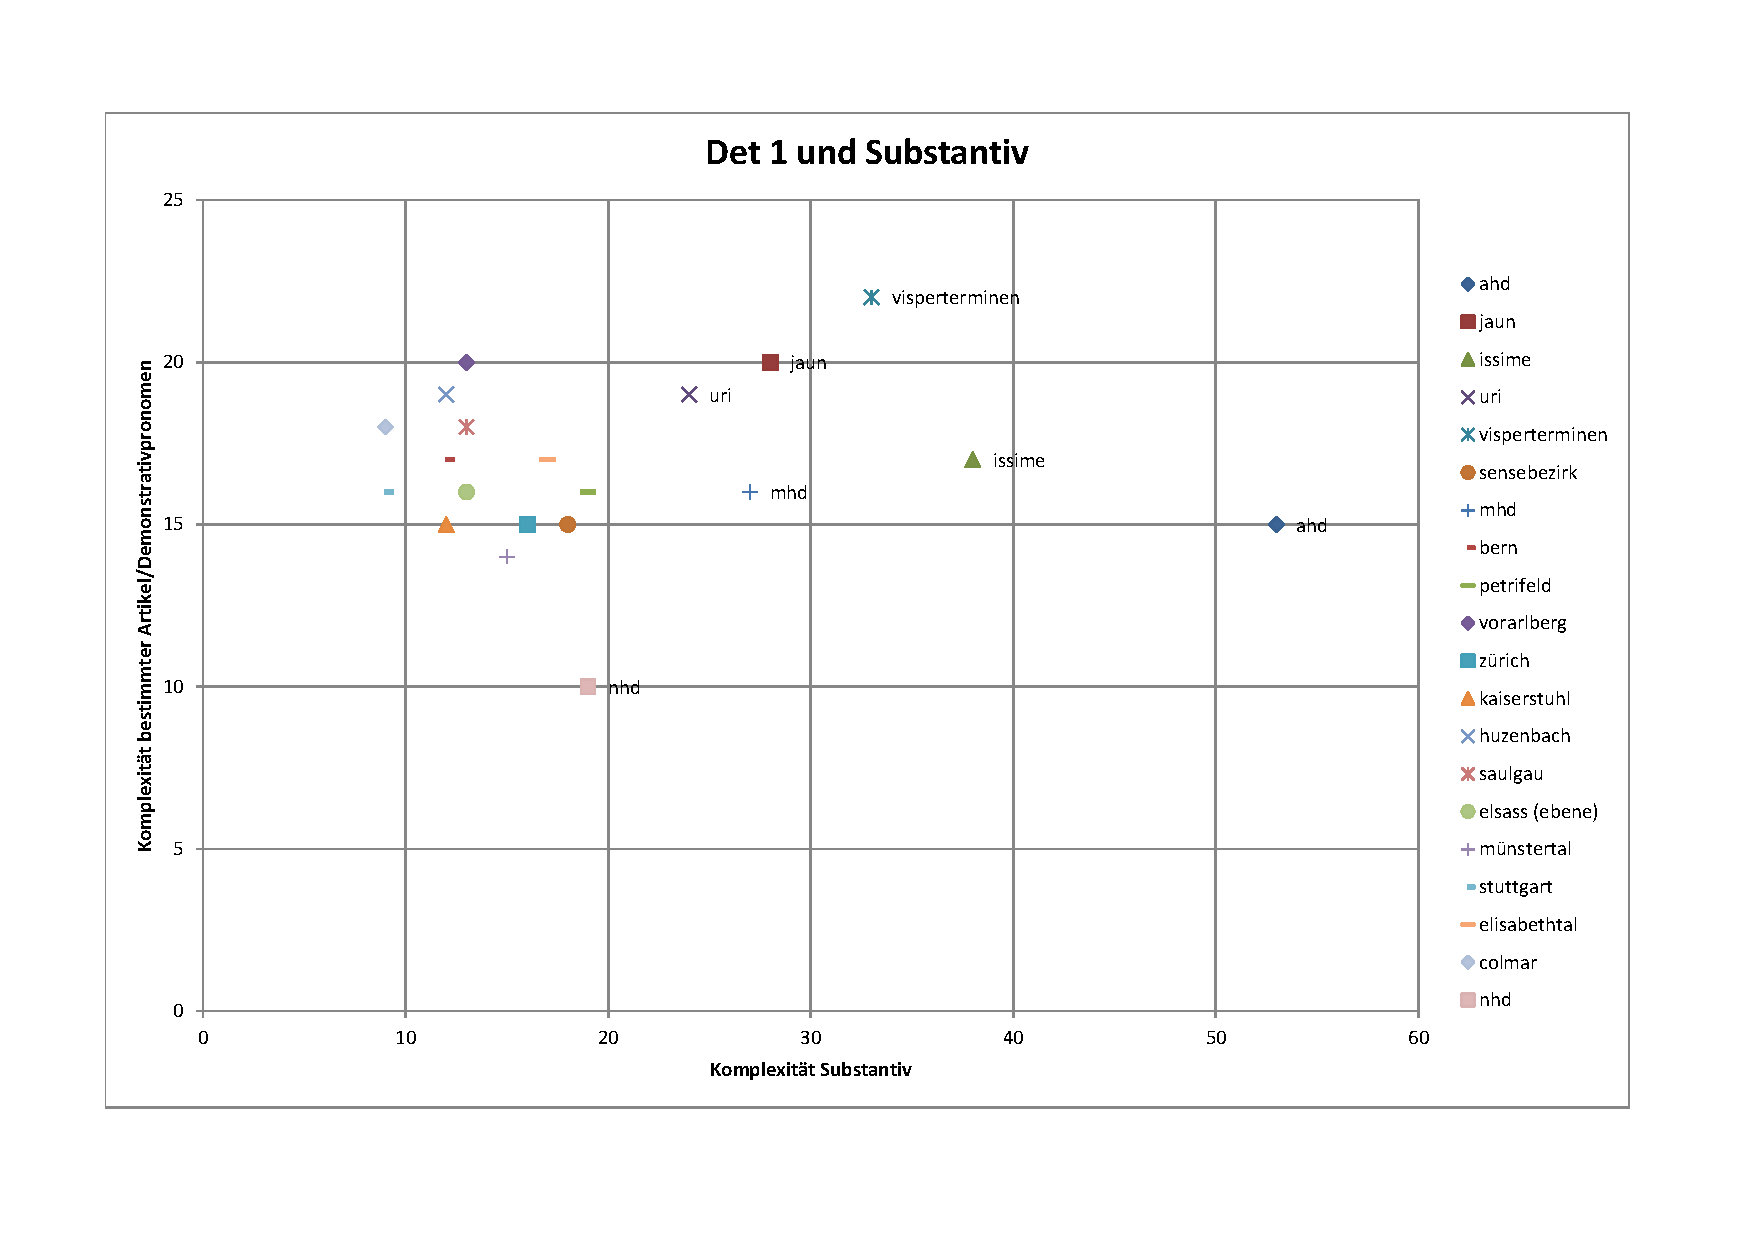
\includegraphics[width=\textwidth]{figures/substDet1.pdf}
    \caption{Komplexität bestimmter Artikel/Demonstrativpronomen + Substantiv}\label{fig:1}
\end{figure}

\begin{figure}
	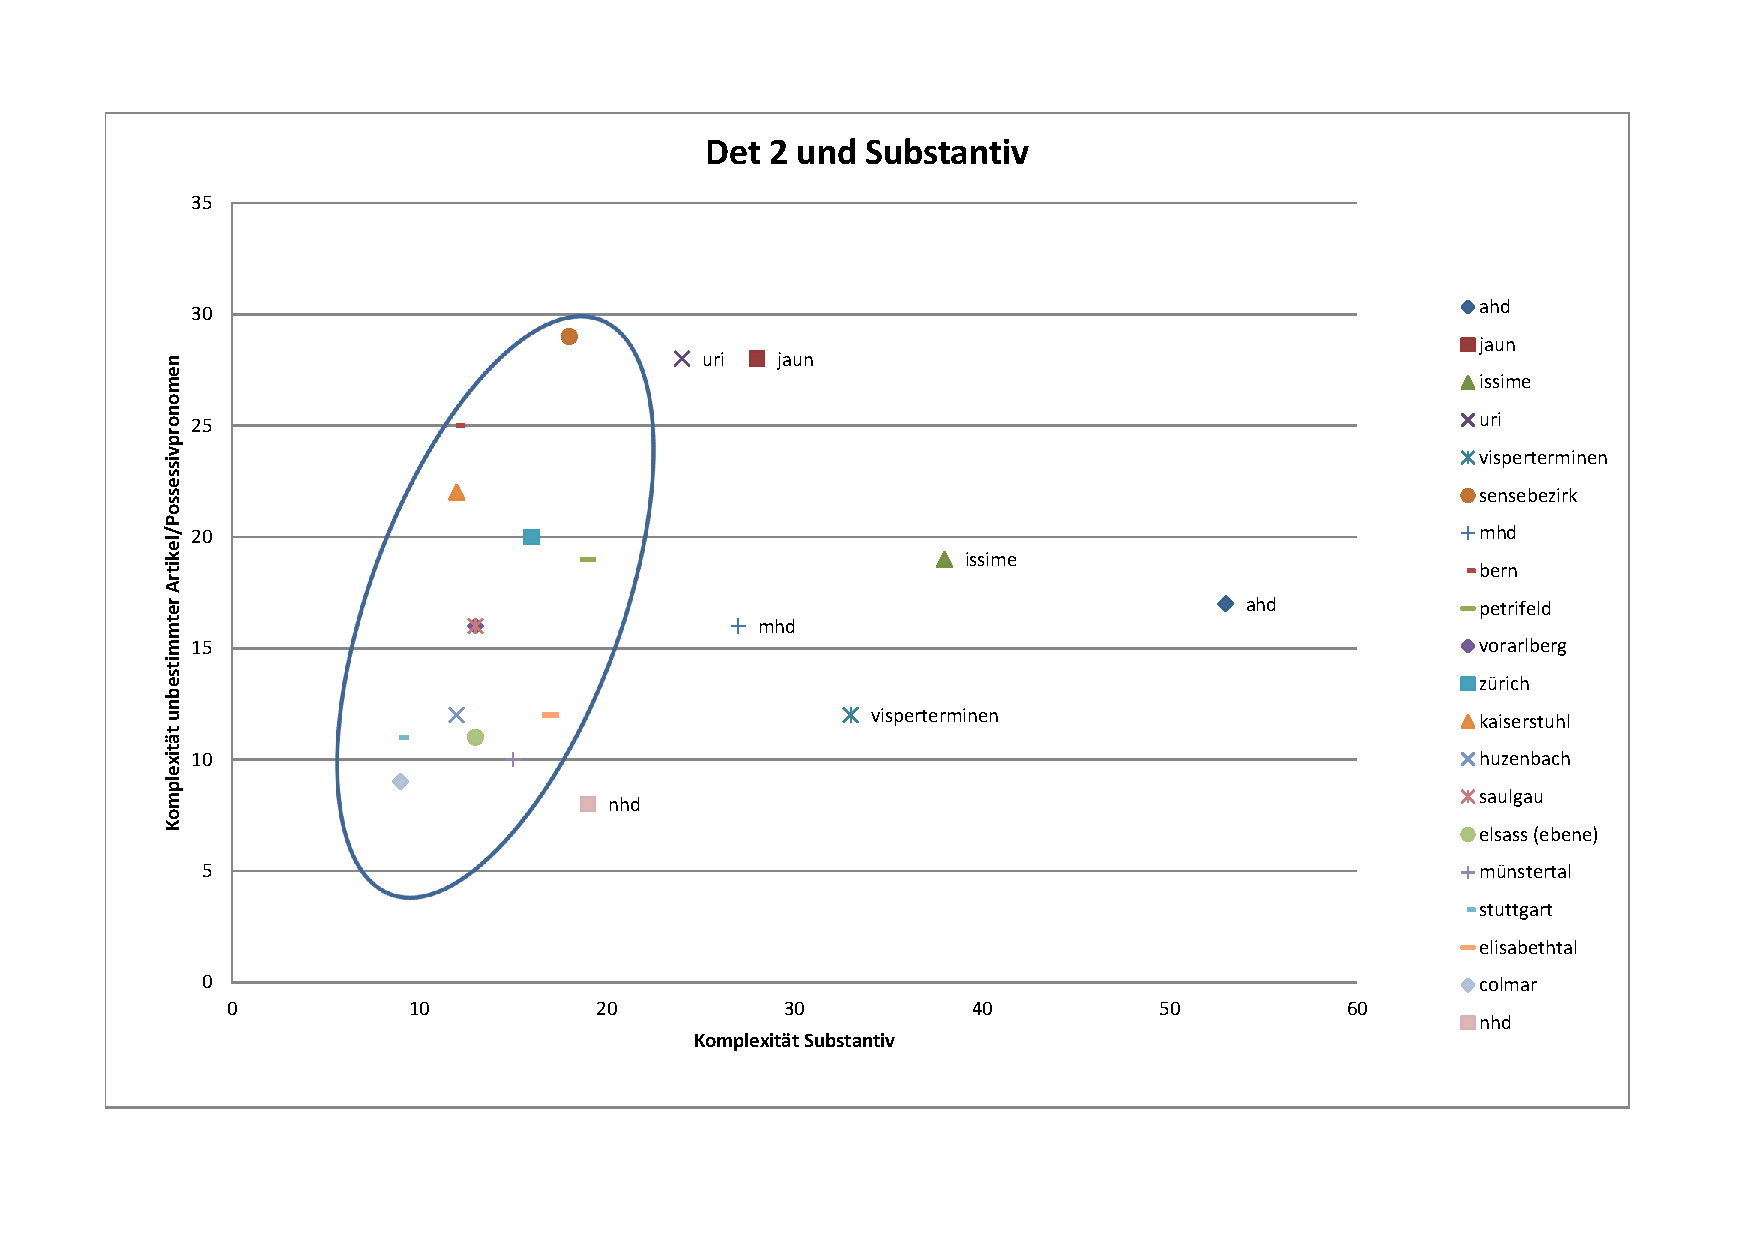
\includegraphics[width=\textwidth]{figures/Det2subst.pdf}
    \caption{Komplexität unbestimmter Artikel / Possessivpronomen + Substantiv}\label{fig:2}
\end{figure}

In \figref{fig:2} ist die Komplexität des Det2 auf der Y-Achse abgebildet, die Komplexität des \isi{Substantivs} auf der X-Achse. Auch hier stellen die Symbole die Varietäten dar. Interessanterweise zeigt \figref{fig:2} ein völlig anderes Bild als \figref{fig:1}, was gegen einen Komplexitätsausgleich zwischen den Determiniererkategorien und dem \isi{Substantiv} spricht. Gäbe es einen Komplexitätsausgleich, würde man wie in \figref{fig:1} erwarten, dass die Varietäten in der Abbildung von oben links nach unten rechts verteilt sind. Möchte man aber in \figref{fig:2} überhaupt eine Tendenz ausmachen, was einigermaßen schwierig ist, da sich die Dialekte verteilen, ist das Gegenteil der Fall: Die Dialekte sind eher von unten links nach oben rechts angeordnet, d.h., dass Varietäten mit einer niedrigeren Komplexität im \isi{Substantiv} auch tendenziell eine niedrigere Komplexität im Det2 aufweisen. Es gibt aber auch einige Parallelen zur \figref{fig:1}. Erstens weist hier die deutsche Standardsprache im Vergleich zu den alemannischen Dialekten ebenfalls eine relativ hohe Komplexität im \isi{Substantiv}, aber geringe Komplexität im Det2 auf. Zweitens haben Jaun und Uri eine vergleichsweise hohe Komplexität im \isi{Substantiv} wie auch im Det2. Anders verhalten sich die Dialekte von Visperterminen und Issime. Beide zeigen eine hohe Komplexität im \isi{Substantiv}, aber eine mittlere (Issime) bzw. eher geringe (Visperterminen) Komplexität im Det2. Folglich finden sich auch bezüglich des Det2 und des \isi{Substantivs} keine Komplexitätsausgleiche.

\subsection{Zusammenfassung}\label{6.1.4}

Zur \isi{Diachronie} lassen sich die wichtigsten Resultate wie folgt zusammenfassen:

\begin{itemize}
\item
Diachrone Simplifizierung wurde in folgenden Kategorien gefunden: Gesamtkomplexität, \isi{Substantive}, \isi{Adjektive} und \isi{Interrogativpronomen}.
\item
Diachrone Komplexifizierung zeigt ungefähr die Hälfte der Dialekte in den folgenden Kategorien: \isi{Personalpronomen}, Det1 und Det2.
\item
Bei den Dialekten, die diachrone Komplexifizierung aufweisen, handelt es sich leicht häufiger um die isolierten ({\textasciitilde}61\%) als um die nicht isolierten Dialekte ({\textasciitilde}47\%). Ein klarerer Zusammenhang konnte jedoch zwischen diachroner Komplexifizierung und einem diatopischen Faktor gefunden werden: Deutlich mehr hoch- (80\%) und höchstalemannische Dialekte ({\textasciitilde}66\%) zeigen diachrone Komplexifizierung als schwäbische ({\textasciitilde}33\%) und oberrheinalemannische Dialekte ({\textasciitilde}17\%).
\end{itemize}

Des Weiteren wurde ein detaillierterer Blick auf die diachronen Mechanismen vorgenommen. Dazu wurde zuerst das Verhältnis zwischen \isi{Archaismen} und \isi{Innovationen} betrachtet, und zwar in den drei Kategorien, die diachrone Komplexifizierung aufweisen. Anschließend wurde dargestellt, dass der Wandel zu einer kooperativen Flexion nicht auf alle Varietäten zutrifft und dass es keinen Komplexitätsausgleich zwischen den Determinierern und den \isi{Substantiven} gibt.

Zum Verhältnis zwischen \isi{Archaismen} und \isi{Innovationen} kann Folgendes festgehalten werden:

\begin{itemize}
\item
Verglichen wurden die Anzahl von \isi{Innovationen} mit dem Kasuserhalt/-abbau in den Kategorien \isi{Personalpronomen}, Det1 und Det2.
\item
Folgende Kombinationen von \isi{Innovationen} und \isi{Archaismen} wurden gefunden (vgl. \tabref{table6.12}): Kasuserhalt + wenig innovativ (Walser Dialekte), Kasuserhalt + sehr innovativ (Jaun), Kasusabbau + (sehr) innovativ (nicht isoliertes Höchstalemannisch, Hochalemannisch), Kasusabbau + wenig innovativ (Oberrheinalemannisch, Schwäbisch).
\item
Dies zeigt, dass es keinen Ausgleich zwischen \isi{Innovationen} und \isi{Archaismen} gibt, d.h. in diesem Fall auch keinen Komplexitätsausgleich.
\item
Welche Dialekte zu welcher Kombination \isi{Innovation}/\isi{Archaismus} gehören, kann nicht aufgrund des Typs der Sprachgemeinschaft, sondern diatopisch bestimmt werden.
\end{itemize}

Schließlich wurde der Wandel zu einer kooperativen Flexion als allgemeines Prinzip für die modernen deutschen Varietäten hinterfragt. Folgendes wurde beobachtet:\largerpage[2]

\begin{itemize}
\item
Alle modernen Varietäten haben einen grammatikalisierten Artikel und eine feste Abfolge in der Nominalphrase.
\item
Die isolierten höchstalemannischen Dialekte haben zusätzlich eine reiche Flexionsmorphologie mit Kasusmarkierung am \isi{Substantiv} erhalten. \isi{Kasus} wird in der Nominalphrase also redundant markiert.
\end{itemize}

\noindent
Daraus kann geschlossen werden, dass:

\begin{itemize}
\item
der grammatikalisierte Artikel und die feste Abfolge in der Nominalphrase auch mit einer reichen Flexionsmorphologie am \isi{Substantiv} vorkommen.
\item
die kooperative Flexion nicht für alle modernen Dialekte gilt. Dabei sei noch darauf hingewiesen, dass jede Varietät in diesem Sample (alt und modern) \isi{Synkretismen} zwischen den Nominalphrasen aufweist.
\end{itemize}

Um zu prüfen, ob es wirklich keinen Ausgleich zwischen den Determinierern und dem \isi{Substantiv} gibt, wurde die Komplexität der \isi{Substantive} jener der Determinierer gegenübergestellt. Zusammenfassend kann Folgendes festgehalten werden (vgl. \figref{fig:1} und \figref{fig:2}):

\begin{itemize}
\item
Die deutsche Standardsprache verhält sich klar anders als die Dialekte. Verallgemeinerungen zu den diachronen Prozessen im Deutschen, die auf dem Vergleich Alt-/Mittelhochdeutsch mit der deutschen Standardsprache basieren, sind also problematisch.
\item
Uri und Jaun: Im \isi{Substantiv} wie auch in den Determiniererkategorien vergleichsweise hohe Komplexität.
\item
Walser Dialekte: Hohe Komplexität im \isi{Substantiv}; Issime mittlere Komplexität im Det1 und Det2; Visperterminen hohe Komplexität im Det1, eher geringe Komplexität im Det2.
\item
Die übrigen Dialekte: Im Det1/\isi{Substantiv} weisen sie gewissen Ähnlichkeiten auf, trotzdem ist die \isi{Variation} zu groß, als dass von einem Komplexitätsausgleich gesprochen werden könnte; Im Det2/\isi{Substantiv} kann beobachtet werden, dass tendenziell Dialekte mit höherer Komplexität am \isi{Substantiv} auch eher höhere Komplexität im Det2 aufweisen.
\end{itemize}

\noindent
Daraus kann geschlossen werden, dass:

\begin{itemize}
\item
die Unterschiede zwischen den Varietäten zu groß sind, als dass ein allgemeines diachrones Prinzip gefunden werden könnte, das für alle modernen Varietäten gilt.
\item
es keinen eindeutigen Komplexitätsausgleich zwischen den Determinierern und den \isi{Substantiven} gibt (Ähnliches wird im folgenden Kapitel gezeigt).
\end{itemize}

\section{Dialektgruppen}\label{6.2}

Im vorangehenden Kapitel konnte gezeigt werden, dass diachrone Komplexifizierung in bestimmten \isi{Dialektgruppen} häufiger vorkommt als in anderen. Berechnet man die durchschnittliche Anzahl der Dialekte pro \isi{Dialektgruppe}, die diachrone Komplexifizierung aufweisen (\tabref{table6.10}), die durchschnittliche Anzahl der diachron komplexifizierten Kategorien pro \isi{Dialektgruppe} (\tabref{table6.11}) sowie die durchschnittliche Anzahl der diachron komplexifizierten Phänomene pro Kategorie und \isi{Dialektgruppe} (\tabref{table6.16}), so wurde immer die gleiche Reihenfolge der \isi{Dialektgruppen} gefunden: Höchstalemannisch > Hochalemannisch > Schwäbisch > Oberrheinalemannisch. Nach diesen diachronen Beobachtungen sollen die \isi{Dialektgruppen} hier synchron verglichen werden, wobei Folgendes im Zentrum steht: Erstens ergibt sich für die \isi{Dialektgruppen} (mit Ausnahme des Schwäbischen) dieselbe Reihenfolge  wie in \sectref{6.1} zur \isi{Diachronie}, betrachtet man die Gesamtkomplexität der einzelnen Dialekte (\tabref{table6.17}). Zweitens gilt dasselbe (mit einzelnen Ausnahmen), wenn man die durchschnittliche Komplexität der einzelnen untersuchten Kategorien und der Gesamtkomplexität pro \isi{Dialektgruppe} berechnet (\tabref{table6.18}). Geschlossen wird das Kapitel mit Überlegungen dazu, was die Resultate für die klassische Einteilung der Dialekte und für die \is{Equi-Complexity-Hypothese}\textit{Equi}{}-\textit{Complexity}{}-Hypothese bedeuten.

\subsection{Beschreibung der Resultate}\label{6.2.1}

\tabref{table6.17} gibt die Gesamtkomplexität (synchron) der untersuchten Dialekte wieder. Daraus wird ersichtlich, dass alle höchstalemannischen Dialekte komplexer sind als alle hochalemannischen und alle hochalemannischen komplexer als alle oberrheinalemannischen. Nur die schwäbischen Dialekte sind verteilt. Petrifeld steht in der hochalemannischen Gruppe, Huzenbach und Saulgau stehen zwischen dem badischen und elsässischen Oberrheinalemannischen und Stuttgart sowie Elisabethtal in der Gruppe des elsässischen Oberrheinalemannischen. Auf den ersten Blick mag dieses sehr klare Ergebnis bezüglich der Reihenfolge von mehr und weniger komplexen \isi{Dialektgruppen} erstaunlich sein. Diese Resultate, also die Komplexität in der nominalen Flexionsmorphologie, bestätigen jedoch die klassische Dialekteinteilung in Höchst-, Hoch- und Niederalemannisch (=Oberrheinalemannisch und Schwäbisch) (mit Ausnahme von Petrifeld, Sprachinsel!).



Um Genaueres zum Schwäbischen im Vergleich zu den anderen \isi{Dialektgruppen} zu erfahren, wurde für jede \isi{Dialektgruppe} das arithmetische Mittel der Komplexität ermittelt. Und zwar wurde dies nicht nur für die Gesamtkomplexität, sondern auch für jede untersuchte Kategorie durchgeführt, um auch diese miteinander vergleichen zu können. Zusammengefasst sind die Resultate in der \tabref{table6.18}.

% % {\tabref{table6.17}: Gesamtkomplexität (\isi{Dialektgruppe})}\\

\begin{table}[]
\caption{Gesamtkomplexität (Dialektgruppe)}\label{table6.17}
\begin{tabular}{llr}
\lsptoprule
% % \multicolumn{3}{l}{{Gesamtkomplexität (alle Kategorien)}}  \\
{DG} & {Varietät} & {Komplexität}\\\midrule
h-st & Jaun & 151\\
h-st & Issime & 141\\
h-st & Uri & 136\\
h-st & Visperterminen & 130\\
h-st & Sensebezirk & 126\\
hoch & Bern & 115\\
schw & Petrifeld & 104\\
hoch & Vorarlberg & 104\\
hoch & Zürich & 103\\
oberr & Kaiserstuhl & 99\\
schw & Huzenbach & 97\\
schw & Saulgau & 95\\
oberr & Elsass (Ebene) & 89\\
oberr & Münstertal & 88\\
schw & Stuttgart & 87\\
schw & Elisabethtal & 87\\
oberr & Colmar & 86\\
\lspbottomrule
\end{tabular}
\end{table}

% % {\tabref{table6.18}: Durchschnittliche Komplexität pro \isi{Dialektgruppe} und Kategorie}\\

\begin{table}[]
\caption{Durchschnittliche Komplexität pro Dialektgruppe und Kategorie}\label{table6.18}
\resizebox{\textwidth}{!}{\begin{tabular}{lS[table-format=2.2]S[table-format=2.2]S[table-format=2.2]S[table-format=2.2]S[table-format=2.2]S[table-format=2.2]S[table-format=2.2]}
\lsptoprule
& \multicolumn{1}{c}{gesamt} & \multicolumn{1}{c}{Det1} & \multicolumn{1}{c}{Det2} & \multicolumn{1}{c}{Pron. inter.} & \multicolumn{1}{c}{Pron. pers.} & \multicolumn{1}{c}{Adj.} & \multicolumn{1}{c}{Nomen}\\\midrule

h-st & 136,2 & 18,6 & 23,2 & 3,8 & 50,4 & 12 & 28,2\\

hoch & 106,67 & 17,34 & 20,34 & 3,67 & 42 & 9,67 & \bfseries 13,67\\

schw & 94 & 17,2 & 14 & \bfseries 5,4 & \bfseries 35,8 & \bfseries 7,6 & \bfseries 14\\

oberr & 90 & 15,75 & 13 & 3,25 & \bfseries 36,5 & \bfseries 9,25 & 12,25\\

\mbox{oberr (Baden)} & 99 & \bfseries 15 & 22 & \bfseries 3 & 37 & 10 & \bfseries 12\\

\mbox{oberr (Elsass)} & 87 & \bfseries 16 & 10 & \bfseries 3,34 & 36,34 & 9 & \bfseries 12,34\\
\lspbottomrule
\end{tabular}}
\end{table}

In der Gesamtkomplexität sind höchstalemannische Dialekte im Durchschnitt komplexer als hochalemannische, hochalemannische komplexer als schwäbische und schwäbische komplexer als oberrheinalemannische. Dasselbe gilt für die Kategorien Det1 sowie Det2. Im \isi{Personalpronomen} und \isi{Adjektiv} bildet Schwäbisch eine Ausnahme, da es weniger komplex als Oberrheinalemannisch ist, wobei der Unterschied besonders im \isi{Personalpronomen} sehr klein ausfällt. Auch im Nomen stellt Schwäbisch eine Ausnahme dar: Es ist komplexer als Hochalemannisch, der Komplexitätsunterschied zwischen diesen beiden \isi{Dialektgruppen} ist aber minimal. Bezüglich des \isi{Interrogativpronomens} wurde bereits in \sectref{6.1.1}) darauf hingewiesen, dass sich die Dialekte in dieser Kategorie nur wenig unterscheiden (vgl. \tabref{table6.2}). Auch hier bildet das Schwäbische eine Ausnahme, weil es komplexer ist als alle anderen \isi{Dialektgruppen}, was vor allem auf die vielen freien Varianten zurückgeführt werden kann (vgl. Paradigmen 72–76). Im Allgemeinen lautet die Komplexitätsreihenfolge folglich Höchstalemannisch > Hochalemannisch > Schwäbisch > Oberrheinalemannisch. Eine Ausnahme hiervon zeigt nur das Schwäbische in einigen Kategorien, jedoch nicht in der Gesamtkomplexität. Die Reihenfolge Höchstalemannisch > Hochalemannisch > Oberrheinalemannisch ist in allen Kategorien und in der Gesamtkomplexität fest.

Es kann hier noch das badische mit dem elsässischen Oberrheinalemannischen verglichen werden (\tabref{table6.18}), auch wenn dieser Vergleich problematisch ist, da das badische Oberrheinalemannisch nur durch einen Dialekt (Kaiserstuhl Alemannisch) vertreten ist. Trotzdem fällt der relativ große Unterschied in der Gesamtkomplexität auf. Dieser kann vorwiegend durch die Resultate der Kategorie Det2 erklärt werden, die ebenfalls einen großen Komplexitätsunterschied zeigt. In allen anderen Kategorien sind die beiden oberrheinalemannischen Untergruppen fast gleich komplex. In der Kategorie Det2 unterscheidet sich das badische vom elsässischen Oberrheinalemannischen vor allem im \isi{Possessivpronomen}: Im Dialekt des Kaiserstuhls (=badisch) verfügt das \isi{Possessivpronomen} über viele freie Varianten im Dativ wie auch über drei unterschiedliche Paradigmen, abhängig von den morphosyntaktischen Eigenschaften des \isi{Possessivpronomens} (vgl. Paradigma 117). Im Gegensatz dazu haben die elsässischen oberrheinalemannischen Dialekte im \isi{Possessivpronomen} keine freien Varianten und nur ein Flexionsparadigma (vgl. Paradigmen 118–120).

\subsection{Analyse und Zusammenfassung}\label{6.2.2}

Aus diesen Ausführungen ergibt sich die folgende Reihenfolge von den komplexeren zu den weniger komplexen \isi{Dialektgruppen}: Höchstalemannisch > Hochalemannisch > Schwäbisch > Oberrheinalemannisch. Nur das Schwäbische weicht in den Kategorien \isi{Personalpronomen}, \isi{Adjektiv} und Nomen davon ab (im \isi{Interrogativpronomen} unterscheiden sich die Dialekte nur sehr wenig). Keine Ausnahmen gibt es bezüglich der Reihenfolge Höchstalemannisch > Hochalemannisch > Oberrheinalemannisch.

Dieses Ergebnis unterstützt klar die traditionelle Einteilung der alemanni-\linebreak schen Dialekte in Höchst-, Hoch- und Oberrheinalemannisch und Schwäbisch.\footnote{Das Bodenseealemannische konnte hier nicht berücksichtigt werden, da für dieses Gebiet keine vollständigen Beschreibungen der Nominalflexion vorhanden sind (vgl. \sectref{3.3.3}).} Diese klassische Einteilung basiert auf phonologischen, morphologischen, syntaktischen und semantischen Isoglossen, die vor allem in den großen Atlasprojekten gefunden wurden. Mit den hier vorgestellten Resultaten kommt ein quantitatives Kriterium aus der Morphologie hinzu: die strukturelle Komplexität der Nominalflexion.

Wichtig sind diese Ergebnisse auch bei der Überprüfung der \is{Equi-Complexity-Hypothese}\textit{Equi}{}-\textit{Complexity}{}-Hypothese. Wären unter dem Strich alle Sprachen/Varietäten gleich komplex, müsste dies nicht nur aus der Gesamtkomplexität, sondern auch aus dem Vergleich der einzelnen Kategorien ersichtlich sein. Wir würden dann bspw. erwarten, dass Dialekt A in der Kategorie X (z.\,B.\ Det1) komplexer als Dialekt B ist, jedoch Dialekt B in der Kategorie Y (z.\,B.\ \isi{Substantiv}) komplexer als Dialekt A. Genau das Gegenteil ist jedoch in den hier vorgestellten Resultaten der Fall: Eine \isi{Dialektgruppe} ist durchschnittlich in jeder Kategorie komplexer als eine andere, die Abfolge von mehr und weniger komplexen \isi{Dialektgruppen} ist in jeder Kategorie dieselbe (mit den genannten Ausnahmen im Schwäbischen). Gewisse \isi{Dialektgruppen} markieren folglich die morphosyntaktischen Eigenschaften innerhalb der Nominalphrase deutlich redundanter als andere \isi{Dialektgruppen}. Ergebnisse, die in dieselbe Richtung gehen, wurden in \sectref{6.1.3} bezüglich der Determinierer und \isi{Substantive} der einzelnen Dialekte gezeigt. Diese Resultate beziehen sich natürlich ausschließlich auf die nominale Flexionsmorphologie. Es kann also hier nicht ausgeschlossen werden, dass der Abbau in der Flexionsmorphologie nicht doch z.\,B.\ in der Syntax ausgeglichen wird. An die vorliegende Arbeit würde sich also eine umfangreiche vergleichende Studie anbieten, die z.\,B.\ die Markierung von Subjekt und direktem Objekt in den unterschiedlichen alemannischen Dialekten untersucht, z.\,B.\ auf eine ähnliche Art und Weise wie \citet{Sinnemäki2008}. Erste exemplarische Arbeiten existieren bereits, wie z.\,B.\ \citet{Ellsäßer2015}.

In der Komplexität der Nominalflexion der hier untersuchten \isi{Dialektgruppen} und Kategorien konnten also keine Ausgleichstendenzen gefunden werden. Das strikte Gegenteil trifft zu. Natürlich können aus diesen Beobachtungen keine allgemeinen Aussagen abgeleitet werden, die für alle Sprache gelten. Dafür bräuchte es ein viel größeres Sample, in dem alle Sprachfamilien adäquat repräsentiert sind. Es sind mir jedoch auch keine Studien bekannt, die das Gegenteil der Resultate dieser Arbeit nachweisen würden bzw. die überhaupt Ausgleichstendenzen zwischen unterschiedlichen Kategorien der Nominalflexion prüfen.

\section{Kontakt}\label{6.3}

Wie in \sectref{2.2.3} dargestellt wurde, kann intensiver \isi{Sprachkontakt} sowohl zu höherer als auch zu niedrigerer Komplexität führen, und zwar abhängig vom Typ der Sprachgemeinschaft. Höhere Komplexität wird in einer sehr langen koterritorialen Kontaktsituation erwartet, in der Kinder zwei- oder mehrsprachig aufwachsen \citep[34]{Trudgill2011}. In Sprachen solcher Sprachgemeinschaften sind \textit{Additive Borrowings} zu beobachten, also Elemente oder Kategorien, die von der einen Sprache in die andere übernommen werden, ohne dass jedoch in der übernehmenden Sprache schon vorhandene Elemente oder Kategorien ersetzt werden \citep[27]{Trudgill2011}. Aus dem untersuchten Sample passen die Sprachinseln Elisabethtal, Petrifeld und Issime sowie die elsässischen Dialekte zu diesem Typ von Sprachgemeinschaft (vgl. Beschreibung der Sprachgemeinschaften dieser Dialekte in \sectref{3.3.3}). Im Gegensatz dazu weisen große Sprachgemeinschaften mit vielen Kontakten, losen Netzwerken und vielen L2-Ler\-nern Simplifizierungen auf \citep[146–147]{Trudgill2011}. In \sectref{3.2.3} wurde argumentiert, dass zur Überprüfung dieser Hypothese Stadt- mit Landdialekten verglichen werden können. Die Stadtdialekte in diesem Sample sind Bern, Zürich (beide Hochalemannisch), Colmar (Oberrheinalemannisch) und Stuttgart (Schwäbisch). Aus dem höchstalemannischen Gebiet gibt es keine vollständige Beschreibung der nominalen Flexionsmorphologie eines Stadtdialekts. Auch die deutsche Standardsprache entspricht jener Sprachgemeinschaft, in der Simplifizierung erwartet wird. Sie wird in \sectref{6.3} gesondert behandelt. Zuerst werden nun die Sprachinseln sowie die elsässischen Dialekte betrachtet und anschließend die Stadt- mit den Landdialekten verglichen.

\subsection{Sprachinseln und Elsass}\label{6.3.1}

In den Sprachinseln Issime, Petrifeld und Elisabethtal sowie in den elsässischen Dialekten sind also \textit{Additive Borrowings} zu erwarten. Interessanterweise wurde aber nur ein \textit{Additive Borrowing} gefunden, und zwar im \isi{Personalpronomen} im Plural des Dialekts von Issime (ausführlich vorgestellt in \sectref{5.3.1}). Zwar weisen Petrifeld, Elisabethtal und die elsässischen Dialekte Lehnwörter aus den jeweiligen Kontaktsprachen auf, diese sind jedoch in das phonologische und morphologische System der alemannischen Dialekte integriert (\citealt[54]{Beyer1963}, \citealt[102–103]{Moser1937}, \citealt[52]{Žirmunskij1928/29}).

Es stellt sich nun die Frage, was Issime von den anderen Sprachinseln und den elsässischen Dialekten unterscheidet. Erstens ist Issime eine deutlich ältere Sprachinsel (seit dem 13. Jh.) als Petrifeld (seit Mitte des 18. Jhs.) und Elisabethtal (seit Anfang des 19. Jhs.). Auch im Elsass breitete sich die deutsch-französische Zweisprachigkeit erst seit der Französischen Revolution allmählich aus (ausführlich in \sectref{3.3.3}). Zweitens setzt ein \textit{Additive Borrowing} voraus, dass die Sprecher bereits als Kinder in beiden Sprachen eine hohe Kompetenz erworben haben, was auf die Alemannischsprecher in Issime zutrifft (vgl. \sectref{3.3.3}). Keine Angaben zur Kompetenz in den Kontaktsprachen, die die Alemannischsprecher von Petrifeld und Elisabethtal hatten (zum Zeitpunkt der Publikation der \isi{Ortsgrammatiken}), konnten gefunden werden. Im Elsass dehnte sich der Bilingualismus erst nach der Französischen Revolution langsam aus, in weiten Bevölkerungsteilen aber erst seit dem Ende des 2. Weltkriegs durch die obligatorische Schule auf Französisch (abgesehen von jenen Sprechern, die einen Sprachwechsel vollzogen haben) (vgl. \sectref{3.3.3}). Im Gegensatz zu den beiden anderen Sprachinseln und den elsässischen Dialekten ist in Issime Mehrsprachigkeit bereits bei Kindern nicht nur gesichert nachweisbar, sondern (im Gegensatz zu den elsässischen Dialekten) seit jeher vorhanden.

Der Dialekt bzw. die Sprachgemeinschaft von Issime bringt also sozusagen die optimalen Voraussetzungen für ein \textit{Additive Borrowing} mit. Es ist jedoch bemerkenswert, dass auch in diesem optimalen Kontext nur ein \textit{Additive Borrowing} vorhanden ist. Zu überlegen ist folglich, ob die \textit{Additive Borrowings} nicht allgemein ein eher seltenes Phänomen darstellen. Das heißt ebenfalls, wie zu erwarten ist, dass die Flexionsmorphologie in Kontaktsituationen deutlich stabiler bleibt als das Lexikon. Dies ist auch daran ersichtlich, dass Petrifeld, Elisabethtal und die elsässischen Dialekte sehr wohl entlehnte Lexeme aus den Kontaktsprachen aufweisen. Andere Studien zeigen jedoch, dass \textit{Additive Borrowings} in bestimmten Kontaktsituationen durchaus üblich sind (vgl. z.\,B.\ \citealt{King2000}). Bezogen auf Issime und auf die Nominalflexion ist jedoch auch zu beachten, dass die Kontaktsprachen nicht viele Möglichkeiten für komplexitätsaufbauende \textit{Additive Borrowings} bieten, da die Kontaktsprachen im Vergleich zu Issime Alemannisch eine eher arme nominale Flexionsmorphologie aufweisen. Was die Kontaktsprachen in der Nominalflexion markieren, markiert Issime sowieso schon (mit der ursprünglichen Ausnahme der Doppelformen im Plural des \isi{Personalpronomens}). Dem Phänomen der \textit{Additive Borrowings} sollte also gesondert genauer nachgegangen werden. Dabei sollte sprachvergleichend vorgegangen werden, aber auch unterschiedliche soziolinguistische Kontexten sollten berücksichtigt werden. Des Weiteren wären auch \textit{Additive Borrowings} auf allen linguistischen Beschreibungsebenen einzubeziehen.

\subsection{Stadtdialekte vs. Landdialekte}\label{6.3.2}

In \sectref{6.2} wurde gezeigt, dass die verschiedenen alemannischen \isi{Dialektgruppen} sich klar in ihrer Komplexität unterscheiden. Deswegen werden hier die Stadt- mit den Landdialekten jeweils innerhalb derselben \isi{Dialektgruppe} verglichen.

Die Resultate des Vergleichs der schwäbischen und oberrheinalemannischen Stadt- und Landdialekte sind in \tabref{table6.19} zusammengefasst, die auf den Resultaten der Tabellen \ref{table6.1}–\ref{table6.3} und \ref{table6.5}–\ref{table6.8} basieren. Das Symbol \ding{52} steht, wenn der Stadtdialekt weniger komplex ist als alle Landdialekte, das Symbol (\ding{52}), wenn der Stadtdialekt und ein Landdialekt dieselbe Komplexität aufweisen und beide weniger komplex sind als alle Landdialekte, das Symbol \ding{55}, wenn der Stadtdialekt nicht weniger komplex ist als alle Landdialekte. Aus der \tabref{table6.19} ist ersichtlich, dass in fünf von sechs Kategorien und in der Gesamtkomplexität der Stadtdialekt weniger komplex ist als die Landdialekte (mit einem Landdialekt derselben Komplexität in einigen Kategorien). Im \isi{Personalpronomen} trifft dies nur auf Colmar zu, im Det1 nur auf Stuttgart und im \isi{Adjektiv} auf keine der beiden Städte. Wir können also festhalten, dass es in den \isi{Dialektgruppen} Oberrheinalemannisch und Schwäbisch zumindest eine Tendenz dazu gibt, dass Stadtdialekte weniger komplex sind als Landdialekte. Dies entspricht \citeauthor{Trudgill2011}s \citeyearpar{Trudgill2011} Annahmen über die Komplexität von Sprachen, die von Sprachgemeinschaften mit vielen Kontakten, losen Netzwerken und vielen L2-Ler\-nern gesprochen werden.

Des Weiteren zeigen sich erstaunliche Parallelen zwischen Schwäbisch und Oberrheinalemannisch. Erstens unterscheiden sich die Resultate dieser \isi{Dialektgruppen} nicht, da generell die Stadtdialekte weniger komplex sind als alle Landdialekte. Eine Ausnahme hiervon bilden nur die Kategorien \isi{Personalpronomen} und Det1 (\tabref{table6.19}). Zweitens sind die Stadtdialekte in den Kategorien \isi{Adjektiv} und Det1 (nur Colmar) komplexer als alle Landdialekte (Tabellen \ref{table6.3} und \ref{table6.8}), im \isi{Personalpronomen} liegt Stuttgart auf dem dritten Platz (von fünf) (\tabref{table6.6}).

% % {\tabref{table6.19}: Stadtdialekt mit geringster Komplexität im Vergleich mit Landdialekten (Schwäbisch und Oberrheinalemannisch)}\\

\begin{table}
\caption{Stadtdialekt mit geringster Komplexität im Vergleich mit Landdialekten (Schwäbisch und Oberrheinalemannisch)}\label{table6.19}
\begin{tabularx}{\textwidth}{lccccccc}
\lsptoprule
& gesamt & Nomen & Det2 & Pron. inter. & Pron. pers. & Det1 & Adj.\\
\midrule
schw & \ding{52} & \ding{52} & \ding{52} & (\ding{52}) & \ding{55} & (\ding{52}) & \ding{55}\\
oberr & \ding{52} & \ding{52} & \ding{52} & (\ding{52}) & (\ding{52}) & \ding{55} & \ding{55}\\
\lspbottomrule
\end{tabularx}
\end{table}

Ganz andere Resultate sind im Hochalemannischen (\tabref{table6.20}) zu beobachten. Hier sind die beiden Stadtdialekte (Bern und Zürich) nur im Det1 und \isi{Adjektiv} weniger komplex als der Dialekt von Vorarlberg. In den meisten Kategorien und in der Gesamtkomplexität steht Vorarlberg zwischen den beiden Stadtdialekten, wobei Bern in mehr Kategorien als Zürich komplexer ist als Vorarlberg. In der Kategorie Det2 zeigt der Dialekt von Vorarlberg sogar die geringste Komplexität verglichen mit den Stadtdialekten. Eine Tendenz wie in den oberrheinalemannischen und schwäbischen Dialekten mit Stadtdialekten von geringerer Komplexität als Landdialekte ergibt sich aus den hier untersuchten hochalemannischen Dialekten nicht. Außerdem gibt es auch bezüglich der Kategorien keine Parallelen zu den oberrheinalemannischen und schwäbischen Dialekten. Eher das Gegenteil trifft zu: Während die oberrheinalemannischen und schwäbischen Stadtdialekte in den Kategorien \isi{Adjektiv} und Det1 (nur Colmar) höhere Komplexität aufweisen als die Landdialekte (\tabref{table6.19}), zeigt Vorarlberg genau in diesen Kategorien eine höhere Komplexität als die Stadtdialekte (\tabref{table6.20}). Ein weiteres Beispiel ist die Kategorie Det2: Die oberrheinalemannischen und schwäbischen Stadtdialekte haben die geringste Komplexität (\tabref{table6.19}), die hochalemannischen Stadtdialekte jedoch die höchste Komplexität (\tabref{table6.20}).

% % {\tabref{table6.20}: Stadt- und Landdialekte im Hochalemannischen}\\

\begin{table}
\caption{Stadt- und Landdialekte im Hochalemannischen}\label{table6.20}
\begin{tabular}{ll}
\lsptoprule
{Reihenfolge Dialekt}
{(mehr – weniger komplex)} & {Kategorie}\\
\midrule
Vorarlberg – Bern – Zürich & Det1\\
& \isi{Adjektiv}\\
\tablevspace
Bern – Vorarlberg – Zürich & Gesamtkomplexität\\
& \isi{Personalpronomen}\\
\tablevspace
& \isi{Interrogativpronomen}\\
Zürich – Vorarlberg – Bern & Nomen\\
\tablevspace
Bern – Zürich – Vorarlberg & Det2\\
\lspbottomrule
\end{tabular}
\end{table}

Für die Hypothese, dass Stadtdialekte eine geringere Komplexität als Landdialekte aufweisen, konnte in den schwäbischen und oberrheinalemannischen Gruppen eine klare Tendenz gefunden werden. Dies gilt jedoch nicht für die hochalemannischen Dialekte. Des Weiteren konnte gezeigt werden, dass sich die schwäbischen und oberrheinalemannischen Stadt- und Landdialekte in den verschiedenen Kategorien sehr ähnlich verhalten. Auch diesbezüglich weicht das Hochalemannische klar vom Schwäbischen und Oberrheinalemannischen ab.

Eine mögliche Erklärung dafür, dass die hochalemannischen Stadtdialekte abweichen, kann im soziolinguistischen Kontext gefunden werden. Dies soll kurz anhand des Vergleichs der hochalemannischen (= Schweizer) Stadtdialekte mit dem schwäbischen (= deutschen) Stadtdialekt veranschaulicht werden. Wenn in Deutschland Sprecher unterschiedlicher Dialekte miteinander kommunizieren, geschieht dies für gewöhnlich in der Standardsprache. Es wird also auf eine dritte Sprache, auf eine Lingua Franca ausgewichen. Folglich ist zu erwarten, dass in den Stadtdialekten viele standardnahe Formen auftreten, sodass Städte und Ballungsgebiete eine Art Insel darstellen. Dies konnte \citet{Pröll2015} für das Untersuchungsgebiet des Sprachatlas von Bayerisch-Schwaben mithilfe geostatistischer Methoden nachweisen: „Sehr deutlich treten die bevölkerungsreichen Orte als eigene, räumlich diskontinuierliche Struktur hervor […]. Wie zu erwarten war, handelt es sich bei den Phänomenen, die diese „städtische“ Tendenz ausmachen, um standardnähere Formen“ (\citealt[160]{Pröll2015}; vgl. auch Faktor 10 in \citealt[146-147]{Pröll2015}). Des Weiteren strahlen Stadtsprachen auf ihre Umgebung aus, was u.a. durch eine hohe Anzahl von Berufspendlern sowie durch ein höheres Prestige der Stadtdialekte im Gegensatz zu den Landdialekten erklärt werden kann. Davon unterscheidet sich die Situation in der Schweiz grundsätzlich. Wenn Sprecher unterschiedlicher Dialekte miteinander kommunizieren, weichen diese nicht auf eine Lingua Franca aus, sondern jeder Beteiligte verwendet seinen eigenen Dialekt, wobei die gegenseitige Verständlichkeit gewährleistet ist. Vermieden werden eventuell besonders kleinräumige Lexeme, die durch großräumigere Lexeme ersetzt werden. Folglich bilden Städte in der Schweiz keine sprachlichen Inseln, die ein höheres Prestige haben oder auf ihre Umgebung ausstrahlen. Auch dies kann durch erste geostatistische Auswertungen des Materials des Sprachatlas der deutschen Schweiz (SDS) und des Syntaktischen Atlas der deutschen Schweiz (SADS) gezeigt werden (Pröll \& Stöckle: in Vorbereitung).\footnote{Ich danke Simon Pröll für die aufschlussreiche Diskussion zu den Unterschieden zwischen den Städten und für den großzügigen Einblick, den er mir ein seine noch unveröffentlichten Daten und Auswertungen gewährt hat.} Um also Genaueres zur eventuellen Rolle der Schweizer Städte zu erfahren, sollten diese mit Landdialekten desselben Dialektgebiets verglichen werden. Dabei sollten Resultate aus geostatistischen Auswertungen als Grundlage zur Bestimmung der Dialektgebiete dienen.

\section{Standardvarietät}\label{6.4}

Für die Hypothese, dass Sprachen von großen Sprachgemeinschaften mit vielen Kontakten, losen Netzwerken und vielen L2-Ler\-nern eher geringere strukturelle Komplexität aufweisen, konnte im vorangehenden Kapitel für das Schwäbische und Oberrheinalemannische eine Tendenz gefunden werden. Dieser Typ Sprachgemeinschaft passt jedoch noch besser zu einer Standardsprache als zu einem Stadtdialekt. Stadtdialekte sind regional gebunden, was vor allem auf die geschriebene deutsche Standardsprache nur in äußerst geringem Maße zutrifft. Die deutsche Standardsprache wird in verschiedenen Ländern verwendet und ist jene Varietät, die besonders im gesteuerten L2-Er\-werb vermittelt wird. Außerdem wird sie von Deutsch-Muttersprachlern mit einem Dialekt als L1 parallel zum Dialekt oder nach dessen Erwerb gelernt (aufgeführt in \sectref{3.2.4}). Schließlich ist das Ziel einer Standardisierung die Vereinheitlichung, woraus eine Vereinfachung resultieren kann. Gleichzeitig kann jedoch die Kodifizierung einer Sprache dazu führen, dass Elemente der Sprache konserviert werden, d.h., auch \isi{Archaismen} mit höherer Komplexität können erhalten werden. Es stellt sich hier folglich die Frage, welche Kraft stärker ist, ob die nominale Flexionsmorphologie der deutschen Standardsprache mehr oder weniger komplex als die untersuchten alemannischen Dialekte ist.

\subsection{Resultate}\label{6.4.1}

In der Gesamtkomplexität ist die deutsche Standardsprache weniger komplex als alle untersuchten Dialekte (\tabref{table6.1}). Dasselbe gilt für die Kategorien Det1, Det2 und das \isi{Personalpronomen} (Tabellen \ref{table6.6}–\ref{table6.8}). Das standarddeutsche \isi{Substantiv} steht in seiner Komplexität im oberen Mittelfeld (\tabref{table6.5}): Mit einem Grad an Komplexität von 19 liegt es leicht über dem arithmetischen Mittel (\={x}=17,78) und am Anfang des oberen Terzils. Dasselbe trifft auf die Anzahl von \isi{Realisierungsregeln} (9) und \isi{Flexionsklassen} (10) zu (\tabref{table6.4}) (\isi{Realisierungsregeln}: \={x}=8,45; \isi{Flexionsklassen} \={x}=9,34). Die Komplexität des \isi{Interrogativpronomens} ist vergleichsweise hoch, wie jedoch bereits erwähnt wurde, unterscheiden sich die untersuchten Varietäten in der Komplexität des \isi{Interrogativpronomens} nur sehr wenig (\tabref{table6.2}). Eine hohe Komplexität weist das  standarddeutsche \isi{Adjektiv} auf (\tabref{table6.3}). Interessanterweise war dies schon bei den oberrheinalemannischen und schwäbischen Stadtdialekten der Fall, jedoch nicht bei den hochalemannischen Stadtvarietäten (vgl. \sectref{6.3}).

\subsection{Analyse}\label{6.4.2}

Es soll nun überlegt werden, wie diese Resultate erklärt werden können und was diese bezüglich der Komplexifizierung und Simplifizierung einer Standardsprache bedeuten. Dazu wird in der Folge jede Kategorie (exklusive \isi{Interrogativpronomen}) einzeln diskutiert.

Wie schon in \sectref{5.5.3} und \sectref{5.6.2} dargestellt wurde, sind die Wortarten der Kategorien {Det1 und Det2} in der Standardsprache weniger weit grammatikalisiert als in den Dialekten. Die Paradigmen des \isi{Demonstrativpronomens} und des \isi{bestimmten Artikels} einerseits (=Det1) und des \isi{Possessivpronomens} und des \isi{unbestimmten Artikels} andererseits (=Det2) unterscheiden sich im Gegensatz zu den dialektalen Paradigmen nicht (vgl. \sectref{5.5.3} und \sectref{5.6.2}). Zur Definition der Paradigmen der Standardsprache ist also nur ein Satz an \isi{Realisierungsregeln} pro Kategorie nötig, während es in den Dialekten pro Kategorie zwei sind. Dass das \isi{Possessivpronomen} einen Plural hat, der \isi{unbestimmte Artikel} jedoch nicht, fällt nicht ins Gewicht, da bei den \isi{Realisierungsregeln} für den Plural die Wortart spezifiziert ist, bei den \isi{Realisierungsregeln} für den Singular jedoch nicht; die Wortart bleibt unterspezifiziert. Des Weiteren weisen die Dialekte unterschiedliche \isi{Innovationen} in den Kategorien Det1 und Det2 auf, die zu höherer Komplexität führen: syntaktisch bedingte Allomorphie (\sectref{5.5.5} und \sectref{5.6.4}), Possessiv-Artikel (\sectref{5.5.2}), unterschiedliche Paradigmen je nach \isi{Possessivpronomen} (\sectref{5.6.6}), Stammalternationen im \isi{Possessivpronomen} (\sectref{5.6.8}) (vgl. \sectref{6.1.3}). Die deutsche Standardsprache weist keine \isi{Innovationen} auf, aus denen eine höhere Komplexität resultiert.

Im {Personalpronomen} unterscheidet die deutsche Standardsprache betonte und unbetonte \isi{Personalpronomen} in der Flexion nicht. Da im Mittel- und Althochdeutschen in der 3. Person betonte und unbetonte \isi{Personalpronomen} verschiedene Formen aufweisen, kann das Fehlen dieser Unterscheidung als diachrone Simplifizierung interpretiert werden. Alle untersuchten Dialekte jedoch haben diese Unterscheidung ausgebaut und verfügen heute über ein vollständiges Paradigma an betonten Formen und über eines an unbetonten Formen (vgl. \sectref{5.3.2} und \sectref{6.1.3}). Einige alemannische Dialekte unterscheiden zusätzlich in der 3. Person Singular Neutrum eine belebte von einer unbelebten Form (vgl. \sectref{5.3.3} und \sectref{6.1.3}). Es handelt sich dabei um eine \isi{Innovation}, die zu höherer Komplexität führt. Wie im Det1 und Det2 weist die deutsche Standardsprache auch im \isi{Personalpronomen} keine solchen \isi{Innovationen} auf.

Im Vergleich zu den alemannischen Dialekten zeigt die deutsche Standardsprache im {Adjektiv} eine hohe Komplexität. Dies ist erstens durch den Erhalt des Genitivs zu erklären, dessen Formen durch \isi{Realisierungsregeln} definiert werden müssen. Mit Ausnahme der isolierten höchstalemannischen Dialekte gibt es in der Adjektivflexion der alemannischen Dialekte keinen Genitiv mehr. Zweitens hat jede Zelle des standardsprachlichen Adjektivparadigmas ein \isi{Suffix}, das durch \isi{Realisierungsregeln} definiert werden muss. Im Gegensatz dazu sind Zellen ohne Endung ein häufiges Phänomen in den alemannischen Dialekten (vgl. Paradigmen 24–40), für die auch keine \isi{Realisierungsregeln} nötig sind, was folglich zu einer niedrigeren Komplexität führt. Zwar konnten \isi{Adjektive} auch im Alt- und Mittelhochdeutschen unflektiert bleiben (= nominale Formen). Allerdings standen diese unflektierten Adjketive mit flektierten \isi{Adjektiven} in derselbe Zelle des Paradigmas in \isi{Variation}. Der Erhalt des Genitivs kann folglich als Konservierung verstanden werden (d.h. hier Erhalt von Komplexität), das Fehlen von unflektierten attributiven \isi{Adjektiven} als Neuerung (d.h. hier Aufbau von Komplexität).

Auch die Komplexität des standardsprachlichen {Substantivs} ist vergleichsweise hoch. Generell wird für die deutsche Standardsprache von einem vier-Kasus-System ausgegangen. Zählt man aber, wie viele \isi{Kasus} maximal pro \isi{Flexionsklasse} markiert werden, so kommt man auf zwei \isi{Kasus} (vgl. \sectref{6.1.3}). Die alemannischen Dialekte jedoch markieren generell am \isi{Substantiv} überhaupt keine \isi{Kasus}.\footnote{Mit wenigen Ausnahmen in Uri (Paradigma 8), Vorarlberg (Paradigma 9), Zürich (Paradigma 10), Petrifeld (Paradigma 15) und Elisabethtal (Paradigma 16).} Eine Ausnahme bilden hier nur die drei isolierten höchstalemannischen Dialekte, die höchstens drei \isi{Kasus} pro \isi{Flexionsklasse} markieren (vgl. \sectref{6.1.3}). Wie in der Adjektivflexion hat die deutsche Standardsprache also auch in der Substantivflexion \isi{Archaismen} bewahrt, die die strukturelle Komplexität erhöhen.

Es ist noch zu klären, ob eventuell eine weitere Ursache für die hohe Komplexität im standarddeutschen \isi{Substantiv} in der Pluralmarkierung liegt. Dazu wurde gezählt, wie viele unterschiedliche Pluralmarker jede moderne Varietät dieses Samples hat. Dabei ist noch zu erwähnen, dass die Nominativ-Plural-Endung genommen wurde, wenn \isi{Numerus} und \isi{Kasus} kumulativ markiert werden, wie z.\,B.\ in Issime: \textit{weg}–\textit{a} (Nominativ/Akkusativ Plural), \textit{weg}–\textit{e} (Dativ Plural), \textit{weg}–\textit{u} (Genitiv Plural) (Zürrer 1999: 164, Paradigma 4). Neben dem Dialekt von Issime kommt dies auch in den Dialekten von Visperterminen, Jaun und Uri vor. Die Resultate sind in der \tabref{table6.21} zusammengefasst. Es zeigt sich, dass die deutsche Standardsprache über eine durchschnittliche Anzahl Pluralmarker verfügt, folglich steht die hohe Komplexität in der standardsprachlichen Substantivflexion nicht mit der Pluralmarkierung in Zusammenhang.

% % {\tabref{table6.21}: Anzahl Pluralmarker pro moderne Varietät}\\

\begin{table}
\caption{Anzahl Pluralmarker pro moderne Varietät}\label{table6.21}
\begin{tabularx}{\textwidth}{cX}
\lsptoprule
{Anzahl Pluralmarker} & {Varietäten}\\
\midrule
3 & Vorarlberg\\
% % \midrule
4 & Bern, Stuttgart, Colmar \\
% % \midrule
5 & Zürich, Huzenbach, Saulgau, Elisabethtal, Kaiserstuhl, Elsass (Ebene), deutsche Standardsprache\\
% % \midrule
6 & Münstertal\\
% % \midrule
7 & Issime, Jaun, Sensebezirk, Petrifeld\\
% % \midrule
8 & Visperterminen, Uri\\
\lspbottomrule
\end{tabularx}
\end{table}

{Zusammengefasst} können wir also Folgendes festhalten: Die deutsche Standardsprache zeigt eine relativ hohe Komplexität in der Adjektiv- und Substantivflexion, was vor allem auf den Erhalt von solchen \isi{Archaismen} zurückzuführen ist, die höhere Komplexität verursachen (z.\,B.\ Kasuserhalt). Gleichzeitig hat die deutsche Standardsprache die niedrigste Komplexität in der Flexion der Kategorien Det1, Det2 und \isi{Personalpronomen}. Zwar hat sie hier im Gegensatz zu den meisten alemannischen Dialekten den Genitiv erhalten. Die alemannischen Dialekte zeigen aber in diesen drei Kategorien zahlreiche \isi{Innovationen}, die zu einem Zuwachs an Komplexität geführt haben. Die deutsche Standardsprache weist keine dieser \isi{Innovationen} auf. Sie kodiert also deutlich weniger Unterscheidungen in der Flexion als die alemannischen Dialekte, was anhand des Fehlens dieser genannten \isi{Innovationen} ersichtlich ist wie auch an der mangelnden Unterscheidung in der Flexion zwischen dem \isi{Demonstrativpronomen} und dem \isi{bestimmten Artikel} einerseits und dem \isi{Possessivpronomen} und dem \isi{unbestimmten Artikel} andererseits. Im Vergleich zu den alemannischen Dialekten ist die deutsche Standardsprache folglich vor allem konservativ: Sie erhält stärker \isi{Archaismen} und zeigt fast keine Neuerungen (mit einer Ausnahme in den \isi{Adjektiven}).\largerpage[2]

Verrechnet man alle berücksichtigten Kategorien, so verfügt die deutsche Standardsprache über die geringste Komplexität in der Nominalflexion. Damit wird zumindest bezüglich dieses Samples die Hypothese bestätigt, dass Sprachen, die von großen Sprachgemeinschaften mit vielen Kontakten, losen Netzwerken und zahlreichen L2-Ler\-nern gesprochen werden, zu einer geringeren strukturellen Komplexität tendieren. Dass die deutsche Standardsprache deutlich weniger Unterscheidungen in der Flexion kodiert als die alemannischen Dialekte (mit Ausnahme der Kasusmarkierung am \isi{Substantiv} und dem Erhalt des Genitivs), also resistenter gegen komplexitätsaufbauende \isi{Innovationen} ist, kann auch vor dem Hintergrund der allgemeinen Anforderungen an einen Standard (z.\,B.\ in der Industrie) verstanden werden: Vereinheitlichung und Vereinfachung ist durchaus das Ziel eines Standards, was bezüglich einer Sprache u.a. die Reduktion von Varianten verursacht. Schließlich verfügt die deutsche Standardsprache nicht über dieselbe diachrone Tiefe wie die Dialekte (vgl. dazu die Diskussion in \sectref{3.2.4}).

\section{Isolation}\label{6.5}

In \sectref{6.3.2} konnte gezeigt werden, dass im Schwäbischen und Oberrheinalemannischen die Stadtdialekte tendenziell eine geringere Komplexität zeigen als die entsprechenden Landdialekte (vgl. \tabref{table6.19}). Auch die deutsche Standardsprache ist weniger komplex als die Dialekte (vgl. \sectref{6.4}). Es kann also angenommen werden, dass große Sprachgemeinschaften mit vielen Kontakten und losen Netzwerken eher eine geringere Komplexität in der Nominalflexion aufweisen. Dies trifft jedoch nicht auf die hochalemannischen Stadtdialekte zu.

In diesem Kapitel soll nun die geografische \isi{Isolation} gesondert betrachtet werden. Bereits in \sectref{6.1} wurden Unterschiede im diachronen Verhalten zwischen isolierten und nicht isolierten Dialekten festgestellt sowie zwischen den verschiedenen \isi{Dialektgruppen}. In diesem Kapitel sollen diese Beobachtungen nun ergänzt und vor allem vertieft werden. Im Fokus steht hier nicht mehr der Vergleich des Alt- bzw. Mittelhochdeutschen mit den modernen Varietäten, sondern der Vergleich von geografisch isolierten und nicht isolierten modernen alemannischen Dialekten, und zwar besonders innerhalb derselben \isi{Dialektgruppe}.

Im hier untersuchten Gebiet impliziert geografische \isi{Isolation}, dass es sich bei diesen Sprachgemeinschaften um kleine und geografisch abgelegene Sprachgemeinschaften handelt mit eher wenigen Kontakten und engen Netzwerken. Folglich werden in diesem Kapitel isolierte Landdialekte mit nicht isolierten Landdialekten und Stadtdialekten verglichen. Welche Dialekte aus welchen Gründen als \isi{geografisch isoliert} gelten können, wurde in \sectref{3.3.3} beschrieben.

In \sectref{6.5.1} wird der Grad der Komplexität der isolierten mit jenem der nicht isolierten Dialekte verglichen, wobei die effektiven Zahlen wie auch Durchschnittswerte berücksichtigt werden. Anschließend wird geprüft, ob sprachinterne Mechanismen (Simplifizierung, Komplexifizierung, Erhalt von \isi{Archaismen}) mit dem einen oder anderen Typ von Sprachgemeinschaft zusammenhängen. Dazu werden zuerst die Kategorien Det1, Det2 und \isi{Personalpronomen} (\sectref{6.5.2}), dann die Kategorien \isi{Adjektiv} und \isi{Substantiv} (\sectref{6.5.3}) analysiert. Geschlossen wird das Kapitel mit einer Synopse (\sectref{6.5.4}).

\subsection{Beschreibung der Resultate}\label{6.5.1}

Zuerst wird der Grad an Komplexität der einzelnen isolierten und nicht isolierten Dialekte verglichen, und zwar jeweils innerhalb der \isi{Dialektgruppe} (\tabref{table6.22}). Zweitens werden die isolierten und die nicht isolierten Dialekte jeder \isi{Dialektgruppe} zusammengenommen und für diese werden Durchschnittswerte errechnet und verglichen (\tabref{table6.23}). Diese Beobachtungen werden in einem dritten Schritt den Resultaten zur diachronen Komplexifizierung isolierter und nicht isolierter Dialekte gegenübergestellt. Die Tabellen \ref{table6.22} und \ref{table6.23} befinden sich am Ende dieses Unterkapitels, gefolgt von \tabref{table6.24}, weil diese Tabellen auch im Zentrum des anschließenden Abschnitts \sectref{6.5.2} stehen.

{Grad der Komplexität von isolierten und nicht isolierten Dialekten:} In \tabref{table6.22} ist der Grad der Komplexität eines jeden isolierten und nicht isolierten alemannischen Dialekts wiedergegeben, und zwar die Gesamtkomplexität der Nominalflexion sowie die Komplexität aller Kategorien. Nur die Resultate des \isi{Interrogativpronomens} wurden hier ausgelassen (in \tabref{table6.2}), da die Komplexitätsunterschiede minimal ausfallen. Aus der \tabref{table6.22} lässt sich Folgendes beobachten: Im Höchstalemannischen sind in allen Kategorien wie auch in der Gesamtkomplexität mindestens zwei von drei isolierte Dialekte komplexer als die nicht isolierten. Eine Ausnahme bildet nur die Kategorie Det2: Hier sind die Walser Dialekte (=isoliert) weniger komplex als die nicht isolierten, und Jaun (=isoliert) steht an zweiter Stelle, also nach dem Dialekt des Sensebezirks und auf gleicher Stufe wie Uri. Wir können folglich festhalten, dass im Höchstalemannischen die isolierten Dialekte eher komplexer sind als die nicht isolierten. Im Hochalemannischen steht der isolierte Dialekt (Vorarlberg) meistens im Mittelfeld. Dies betrifft die Gesamtkomplexität wie auch die Kategorien \isi{Personalpronomen}, \isi{Adjektiv} und \isi{Substantiv}. Komplexer als die nicht isolierten Dialekte ist der Dialekt von Vorarlberg in der Kategorie Det1, weniger komplex in der Kategorie Det2. Auch im Schwäbischen steht der isolierte Dialekt (Huzenbach) in der Gesamtkomplexität im Mittelfeld. Im Gegensatz zu Vorarlberg gibt es im Dialekt von Huzenbach in den übrigen Kategorien jedoch große Unterschiede. Am komplexesten im Vergleich zu den nicht isolierten Dialekten ist der Dialekt von Huzenbach in den Kategorien Det1 und \isi{Personalpronomen}. In der Kategorie \isi{Adjektiv} zeigt er jedoch die geringste Komplexität verglichen mit den nicht isolierten Dialekten, in den Kategorien Det2 und \isi{Substantiv} die zweit geringste. Der Dialekt von Huzenbach variiert folglich sehr stark in seiner Komplexität zwischen den verschiedenen Kategorien. Auch im Oberrheinalemannischen scheint die \isi{Variation} zuerst groß. Die höchste Komplexität (verglichen mit den nicht isolierten Dialekten) zeigt der Dialekt von Münstertal (=isoliert) in den Kategorien \isi{Substantiv} und \isi{Personalpronomen}, die geringste Komplexität im \isi{Adjektiv} und Det1, die zweitgeringste im Det2. Auch in der Gesamtkomplexität steht Münstertal auf dem zweitletzten Platz. Jedoch ist hier hervorzuheben, dass die Unterschiede in der Gesamtkomplexität vor allem der elsässischen Dialekte sehr gering ausfallen.

Daraus können wir Folgendes festhalten: Erstens gibt es ein eindeutiges Resultat nur in den höchstalemannischen Dialekten. Hier sind die isolierten Dialekte generell komplexer als die nicht isolierten. Eine eindeutige Tendenz konnte für die übrigen \isi{Dialektgruppen} nicht gefunden werden. Zweitens ist die \isi{Variation} in Bezug darauf, wie sich die isolierten und nicht isolierten Dialekte in den verschiedenen Kategorien zueinander verhalten, zwischen den verschiedenen \isi{Dialektgruppen} groß, d.h., ein sich wiederholendes Muster konnte hier nicht herausgearbeitet werden. Drittens zeigt der Vergleich der Kategorien \isi{Personalpronomen}, Det1 und Det2 jedoch ein klareres Bild: In drei von vier \isi{Dialektgruppen} zeigt der isolierte Dialekt die höchste Komplexität in den Kategorien Det1 (nicht Oberrheinalemannisch) und \isi{Personalpronomen} (nicht Hochalemannisch), während in der Kategorie Det2 nicht ein einziger isolierte Dialekt die höchste Komplexität hat.

{Durchschnittliche Komplexität von isolierten und nicht isolierten Dialekten:} Da die Komplexitätsvariation der isolierten und nicht isolierten Dialekte auf den ersten Blick sehr groß erscheint, wurde die durchschnittliche Komplexität für die isolierten Dialekte einerseits und für die nicht isolierten Dialekte andererseits für jede \isi{Dialektgruppe} und Kategorie berechnet. Damit bekommt man die Daten besser in den Griff. Diese Durchschnittswerte sind in der \tabref{table6.23} zusammengefasst. Außerdem steht in der rechtesten Spalte dieser Tabelle, wie viele Kategorien (insgesamt fünf) in den isolierten Dialekten eine höhere Komplexität aufweisen als in den nicht isolierten Dialekten und umgekehrt. Zudem befinden sich in den untersten zwei Spalten zwei Zahlen. Die erste Zahl gibt die durchschnittliche Komplexität jeder Kategorie sowie von der Gesamtkomplexität aller Dialekte wieder, also unabhängig von der \isi{Dialektgruppe}. Die zweite Zahl zeigt pro Kategorie und Gesamtkomplexität, in wie vielen \isi{Dialektgruppen} (von insgesamt vier) die isolierten und nicht isolierten Dialekte durchschnittlich eine höhere Komplexität aufweisen. Zuerst wird nun die durchschnittliche Komplexität von isolierten und nicht isolierten Dialekten innerhalb derselben \isi{Dialektgruppe} verglichen (horizontaler Vergleich in \tabref{table6.23}). Zweitens werden die Durchschnittswerte der Kategorien einander gegenübergestellt (vertikaler Vergleich in \tabref{table6.23}).

Im Höchstalemannischen zeigen die isolierten Dialekte eine durchschnittlich höherer Gesamtkomplexität als die nicht isolierten Dialekte. Dasselbe gilt für alle Kategorien außer der Kategorie Det2: Hier sind die nicht isolierten Dialekte deutlich komplexer als die isolierten. Es kann aber festgehalten werden, dass im Höchstalemannischen die isolierten Dialekte meistens komplexer sind als die nicht isolierten. Auch im Schwäbischen hat der isolierte Dialekt eine höhere Gesamtkomplexität als die nicht isolierten Dialekte. Dasselbe ist für das \isi{Personalpronomen} und den Det1 zu beobachten. Eine geringere Komplexität als die nicht isolierten Dialekte weist der isolierte Dialekt im \isi{Adjektiv}, \isi{Substantiv} und Det2 auf (Det2 wie im Höchstalemannischen). Zusammengefasst zeigt also der isolierte schwäbische Dialekt (wie die höchstalemannischen) eine höhere Gesamtkomplexität als die nicht isolierten. Im Gegensatz zu den höchstalemannischen isolierten Dialekten jedoch hat der isolierte schwäbische Dialekt nur in zwei von fünf Kategorien eine höhere Komplexität als die nicht isolierten. Dasselbe kann in den hoch- und oberrheinalemannischen Dialekten beobachtet werden: In zwei von fünf Kategorien sind die isolierten Dialekte komplexer als die nicht isolierten Dialekte, in drei von fünf Kategorien die nicht isolierten komplexer als die isolierten. Im Gegensatz zum Schwäbischen weisen die isolierten hoch- und oberrheinalemannischen Dialekte aber auch in ihrer Gesamtkomplexität einen geringeren Wert auf als die nicht isolierten.

Vergleicht man also die durchschnittlichen Komplexitätswerte von isolierten und nicht isolierten Dialekten, kann Folgendes konstatiert werden: Erstens weisen im Höchstalemannischen die isolierten Dialekte generell eine höhere Komplexität auf als die nicht isolierten (Ausnahme im Det2). Zweitens ist die Situation in den schwäbischen, hoch- und oberrheinalemannischen Dialekten ausgeglichener: In zwei von fünf Kategorien (+ Gesamtkomplexität im Schwäbischen) sind die isolierten Dialekte komplexer als die nicht isolierten, in drei von fünf Kategorien (+ Gesamtkomplexität im Hoch- und Oberrheinalemannischen) sind die nicht isolierten komplexer als die isolierten. Diese Beobachtungen bezüglich der Durchschnittswerte entsprechen der Intuition zu den effektiven Zahlen (\tabref{table6.22}). Drittens variieren die einzelnen Kategorien sehr stark: In welcher Kategorie die isolierten oder nicht isolierten Dialekte (von welcher \isi{Dialektgruppe}) höhere oder niedrigere Komplexität aufweisen, ist nicht eindeutig vorauszusagen (Genaueres dazu folgt unten). Eine Ausnahme bildet hier nur die Kategorie Det2, in der die nicht isolierten Dialekte stets komplexer sind als die isolierten.

Im Höchstalemannischen weisen die isolierten Dialekte also generell eine höhere Komplexität auf als die nicht isolierten, während eine solche Aussagen in den übrigen drei \isi{Dialektgruppen} nicht möglich ist. Vergleicht man nun die Gesamtkomplexität der isolierten und nicht isolierten Dialekte unabhängig von der \isi{Dialektgruppe}, wird ebenfalls ein eher ambivalentes Ergebnis erkennbar. Wie bereits beschrieben wurde, zeigen in zwei von vier \isi{Dialektgruppen} die isolierten Dialekte eine höhere Komplexität als die nicht isolierten und umgekehrt. Berechnet man jedoch den Durchschnittswert, so sind die isolierten Dialekte leicht komplexer (107,08) als die nicht isolierten (103,06) (vgl. \tabref{table6.23}). Hier muss jedoch erwähnt werden, dass von den sechs isolierten Dialekten in diesem Sample drei zum Höchstalemannischen gehören, wodurch das Höchstalemannische überrepräsentiert ist. Dazu kommt, dass das Höchstalemannische (unabhängig von der Isoliertheit) generell komplexer ist als die übrigen \isi{Dialektgruppen}, wie dies in \sectref{6.2} dargestellt wurde.

Nun sollen noch die Durchschnittswerte der einzelnen Kategorien miteinander verglichen werden (vertikaler Vergleich in \tabref{table6.23}). In den Kategorien \isi{Personalpronomen}, Det1, \isi{Adjektiv} und \isi{Substantiv} zeigen die isolierten Dialekte durchschnittlich eine etwas höhere Komplexität als die nicht isolierten. Das Gegenteil trifft nur auf die Kategorie Det2 zu. Wie schon erwähnt wurde, kann dies mit der Überrepräsentation des Höchstalemannischen unter den isolierten Dialekten zusammenhängen. Deswegen ist es interessanter zu prüfen, in welchen Kategorien in wie vielen \isi{Dialektgruppen} die isolierten Dialekte mehr oder weniger komplex sind als die nicht isolierten. Im \isi{Adjektiv} und \isi{Substantiv} ist das Verhältnis ausgeglichen: in zwei von vier \isi{Dialektgruppen} weisen die isolierten Dialekte eine höhere Komplexität auf als die nicht isolierten und umgekehrt. Ganz anders sieht dies in den übrigen drei Kategorien aus. Im \isi{Personalpronomen} und Det1 haben in drei von vier \isi{Dialektgruppen} die isolierten Dialekte eine höhere Komplexität als die nicht isolierten, während in der Kategorie Det2 in allen \isi{Dialektgruppen} die nicht isolierten Dialekte eine höhere Komplexität aufweisen als die isolierten. Außerdem ist in der Kategorie Det2 der Komplexitätsunterschied zwischen isolierten und nicht isolierten Dialekten in allen \isi{Dialektgruppen} größer als in den anderen Kategorien. Wir können also festhalten, dass das Verhältnis zwischen isolierten und nicht isolierten Dialekten bezüglich höherer/niedrigerer Komplexität zwischen den Kategorien stark variiert, und zwar besonders in den Kategorien \isi{Personalpronomen}, Det1 und Det2.

{Vergleich der Durchschnittswerte mit der diachronen Komplexifizierung:} Letztere Beobachtung erinnert an die Ergebnisse aus \sectref{6.1.2} bezüglich der diachronen Komplexifizierung, denn nur in den Kategorien \isi{Personalpronomen}, Det1 und Det2 zeigen etliche alemannische Dialekte eine höhere Komplexität als ihr diachrones Pendant (vgl. Tabellen \ref{table6.6}–\ref{table6.8}). Für diese drei Kategorien wurde in \sectref{6.1.2} berechnet, wie viele isolierte und nicht isolierte Dialekte durchschnittlich diachrone Komplexifizierung aufweisen, also komplexer sind als ihr diachrones Pendant. Die Resultate wurden in der \tabref{table6.9} zusammengefasst. Diese werden nun mit der durchschnittlichen Komplexität (\tabref{table6.23}) verglichen.

Aus der \tabref{table6.9} ist zu lesen, dass prozentual mehr isolierte Dialekte im \isi{Personalpronomen} und Det1 diachrone Komplexifizierung aufweisen als die nicht isolierten Dialekte (\isi{Personalpronomen}: 66\% vs. 25\%; Det1: 83\% vs. 66\%). Das Gegenteil trifft auf die Kategorie Det2 zu: Weniger isolierte als nicht isolierte Dialekte zeigen diachrone Komplexifizierung (33\% vs. 50\%). Wie zu erwarten ist, kann Ähnliches in der \tabref{table6.23} beobachtet werden. Die durchschnittliche Komplexität der isolierten Dialekte ist in den Kategorien \isi{Personalpronomen} und Det1 höher als jene der nicht isolierten Dialekte (\isi{Personalpronomen}: 42,67 vs. 40,77; Det1: 18,17 vs. 16,52), aber geringer in der Kategorie Det2 (14,42 vs. 19,88). Hier ist natürlich zu berücksichtigen, dass, wie bereits erwähnt wurde, die höchstalemannischen Dialekte unter den isolierten Dialekten überrepräsentiert sind. Unterstützt werden diese Resultate jedoch, wenn man zählt, in wie vielen \isi{Dialektgruppen} die isolierten Dialekte eine höhere Komplexität haben als die nicht isolierten (wobei sich das Problem der Überrepräsentation der höchstalemannischen isolierten Dialekte nicht mehr stellt): In den Kategorien \isi{Personalpronomen} und Det1 zeigen die isolierten Dialekte in drei von vier \isi{Dialektgruppen} eine höhere Komplexität als die nicht isolierten Dialekte, während in der Kategorie Det2 stets die nicht isolierten Dialekte eine höhere Komplexität aufweisen als die isolierten Dialekte.

{Zusammenfassung:} Diese zahlreichen Ergebnisse sollen hier kurz zusammengefasst werden, um anschließend ein Fazit zu ziehen, woraus sich neue Fragen ergeben. Diese werden in den sich anschließenden Abschnitten beantwortet.

Die wichtigsten Resultate lassen sich wie folgt zusammenfassen und beziehen sich auf die \tabref{table6.23} (Durchschnittswerte).

\begin{description}
 \item[Gesamtkomplexität:]
 
\begin{itemize}
\item[]
\item
Im Höchstalemannischen und Schwäbischen zeigen die isolierten\linebreak Dialekte eine höhere Gesamtkomplexität als die nicht isolierten Dialekte. Das Gegenteil trifft auf das Hoch- und Oberrheinalemannische zu.
\item
Unabhängig von den \isi{Dialektgruppen} sind die isolierten Dialekte in ihrer Gesamtkomplexität etwas komplexer (107,08) als die nicht isolierten (103,06). Hier ist zu berücksichtigen, dass das Höchstalemannische unter den isolierten Dialekten überrepräsentiert ist.
\item
Daraus kann geschlossen werden: Einen einfachen, klaren Zusammenhang zwischen geografischer \isi{Isolation} und Komplexität gibt es in diesem Sample nicht.
\end{itemize}

\item[Komplexität der einzelnen Kategorien:]
\begin{itemize}
\item[]
\item
Das isolierte Höchstalemannisch hat in vier von fünf Kategorien eine höhere Komplexität als das nicht isolierte. In den anderen \isi{Dialektgruppen} trifft dies nur auf zwei von fünf Kategorien der isolierten Dialekte zu.
\item
Bezüglich des \isi{Adjektivs} und des \isi{Substantivs} zeigen die isolierten Dialekte in zwei von vier \isi{Dialektgruppen} eine höhere Komplexität als die nicht isolierten, bezüglich des \isi{Personalpronomens} und des Det1 in drei von vier \isi{Dialektgruppen}, bezüglich des Det2 in keiner \isi{Dialektgruppe}.
\item
Diese Resultate des \isi{Personalpronomens}, Det1 und Det2 werden\linebreak durch die durchschnittliche Anzahl isolierter Dialekte mit diachroner Komplexifizierung (\tabref{table6.9}) unterstützt.
\item
Daraus kann geschlossen werden: a) Eine klare Tendenz gibt es nur im Höchstalemannischen, in den übrigen \isi{Dialektgruppen} ist die Situation ausgeglichener; b) Zwischen den Kategorien gibt es große \isi{Variation} in Bezug darauf, ob eher die isolierten oder die nicht isolierten Dialekte eine höhere Komplexität aufweisen.
\end{itemize}
\end{description}

Gerade der unklare Zusammenhang zwischen \isi{Isolation} und Komplexität sowie die große \isi{Variation} zwischen den Kategorien scheinen besonders interessant. Es stellt sich nämlich die Frage, welche sprachinternen Mechanismen für die große \isi{Variation} zwischen den Kategorien verantwortlich sind. Oder anders gefragt: Gibt es sprachinterne Mechanismen, die eher in isolierten Dialekten zu beobachten sind, und andere, die eher in nicht isolierten Dialekten vorkommen? Denn die hier verwendete Methode zur Messung struktureller Komplexität verrechnet die unterschiedlichen Mechanismen miteinander, was auch erwünscht ist und wodurch gezeigt werden konnte, dass unter dem Strich nicht alle hier untersuchten Varietäten gleich komplex sind. Trotzdem soll tiefer im Sprachsystem gegraben werden, um einen Zusammenhang zwischen sprachinternen Mechanismen und \isi{Isolation} zu prüfen.

Für die Ziele dieser Arbeit lässt sich der morphologische Sprachwandel stark vereinfacht in zwei Typen aufteilen. Sprachwandel kann zu niedrigerer Komplexität führen, indem z.\,B.\ Formen des Paradigmas zusammenfallen. Im Extremfall fallen so ganze morphosyntaktische Kategorien weg, wie z.\,B.\ der Verlust des Genitivs oder überhaupt der Kasusmarkierung an sich. Davon können einzelne Wortarten oder das gesamte Sprachsystem betroffen sein. Im anderen Typ von Sprachwandel werden neue Kategorien unterschieden, beispielsweise die \isi{Betontheit} im \isi{Personalpronomen} der alemannischen Dialekte. \citet{Trudgill2011} geht davon aus, dass nicht isolierte Dialekte eher von jenem Typ Sprachwandel betroffen sind, der das System vereinfacht. In \isi{isolierten Sprachgemeinschaften} ist der Sprachwandel hingegen langsamer, was den Erhalt von komplexeren Phänomenen zur Konsequenz hat, die in nicht isolierten Varietäten abgebaut werden. Zudem führt der Sprachwandel in den \isi{isolierten Sprachgemeinschaften} eher zu höherer Komplexität (ausführlich in \sectref{2.2.3} dargestellt). In den folgenden zwei Unterkapiteln soll also geprüft werden, ob in den isolierten Dialekten eher \isi{Archaismen} und Resultate eines Sprachwandels, der zu höherer Komplexität führt, zu finden sind, während in nicht isolierten Dialekten eher Neuerungen mit geringerer Komplexität erwartet werden. Zuerst werden die Kategorien \isi{Personalpronomen}, Det1 und Det2 analysiert, anschließend die \isi{Adjektive} und \isi{Substantive}. Erste Hinweise und Resultate wurden bereits in \sectref{6.1} besprochen. Hier soll nun eine deutlich detailliertere Analyse folgen, und zwar mit einem Fokus auf den alemannischen Dialekte.

% % {\tabref{table6.22}: Höhe der Komplexität der Dialekte in allen Kategorien (außer \isi{Interrogativpronomen})}

\begin{table}
\caption{Höhe der Komplexität der Dialekte in allen Kategorien (außer Interrogativpronomen)}\label{table6.22}
\resizebox{\textwidth}{!}{\begin{tabular}{lrrrrrr}
\lsptoprule
& \multicolumn{1}{p{2cm}}{Gesamt\-kom\-plexi\-tät} & \multicolumn{1}{p{2cm}}{Per\-so\-nal\-pro\-no\-men} & {Det1} & {Det2} & {Adjektiv} & {Substantiv}\\
\midrule
\multicolumn{7}{c}{Höchstalemannisch}\\\midrule
Jaun & 151 & 55 & 20 & 29 & 15 & 28\\
Issime & 141 & 52 & 17 & 19 & 11 & 38\\
Visperterminen & 130 & 45 & 22 & 12 & 14 & 33\\
Uri & 136 & 51 & 19 & 29 & 9 & 24\\
Sensebezirk & 126 & 49 & 15 & 30 & 11 & 18\\
\midrule
\multicolumn{7}{c}{Hochalemannisch} \\\midrule
Vorarlberg & 104 & 41 & 20 & 16 & 10 & 13\\
Zürich & 103 & 39 & 15 & 21 & 9 & 16\\
Bern & 115 & 46 & 17 & 26 & 10 & 12\\
\midrule
\multicolumn{7}{c}{Schwäbisch}  \\\midrule
Huzenbach & 97 & 42 & 19 & 12 & 6 & 12\\
Saulgau & 95 & 35 & 18 & 16 & 8 & 13\\
Stuttgart & 87 & 36 & 16 & 11 & 10 & 9\\
Petrifeld & 104 & 37 & 16 & 19 & 7 & 19\\
Elisabethtal & 87 & 29 & 17 & 12 & 7 & 17\\
\midrule
\multicolumn{7}{c}{Oberrheinalemannisch} \\\midrule
Münstertal & 88 & 37 & 14 & 11 & 8 & 15\\
\mbox{Elsass (Ebene)} & 89 & 36 & 16 & 12 & 8 & 13\\
Colmar & 86 & 36 & 18 & 9 & 11 & 9\\
Kaiserstuhl & 99 & 37 & 15 & 22 & 10 & 12\\
\lspbottomrule
\end{tabular}}
\end{table}

% % {\tabref{table6.23}: Durchschnittliche Komplexität der isolierten und nicht isolierten Dialekte pro \isi{Dialektgruppe} (Zahl} {= nicht isoliert komplexer als isoliert)}

\begin{table}
\caption{Durchschnittliche Komplexität der isolierten und nicht isolierten Dialekte pro Dialektgruppe ({\underline{Zahl}} = nicht isoliert komplexer als isoliert)}\label{table6.23}
\resizebox{\textwidth}{!}{\begin{tabular}{lSSSSSSSSSSSSS}
\lsptoprule
% % & \multicolumn{12}{l}{{Durchschnittliche Komplexität (arithmetisches Mittel)}} & \\
& \multicolumn{2}{p{2cm}}{Gesamt\-kom\-plexi\-tät} & \multicolumn{2}{p{2cm}}{Per\-so\-nal\-pro\-no\-men} & \multicolumn{2}{l}{{Det1}} & \multicolumn{2}{l}{{Det2}} & \multicolumn{2}{l}{{Adjektiv}} & \multicolumn{2}{l}{{Substantiv}} & \multicolumn{1}{p{2cm}}{Anzahl von Kategorien mit höherer Komplexität}\\
\midrule
\multicolumn{14}{c}{{Höchstalemannisch}} \\\midrule

isoliert & \multicolumn{2}{l}{140,34} & \multicolumn{2}{l}{50,67} & \multicolumn{2}{l}{\underline{19,67}} & \multicolumn{2}{l}{19,67} & \multicolumn{2}{l}{13,34} & \multicolumn{2}{l}{33} & 4/5 + gesamt\\

nicht isoliert & \multicolumn{2}{l}{120} & \multicolumn{2}{l}{50} & \multicolumn{2}{l}{17} & \multicolumn{2}{l}{\underline{28,5}} & \multicolumn{2}{l}{10} & \multicolumn{2}{l}{21} & 1/5\\
\midrule
\multicolumn{14}{c}{{Hochalemannisch}}  \\\midrule

isoliert & \multicolumn{2}{l}{\underline{104}} & \multicolumn{2}{l}{\underline{41}} & \multicolumn{2}{l}{20} & \multicolumn{2}{l}{\underline{16}} & \multicolumn{2}{l}{10} & \multicolumn{2}{l}{\underline{13}} & 2/5\\

nicht isoliert & \multicolumn{2}{l}{\underline{108}} & \multicolumn{2}{l}{\underline{42,5}} & \multicolumn{2}{l}{16} & \multicolumn{2}{l}{\underline{22,5}} & \multicolumn{2}{l}{9,5} &  \multicolumn{2}{l}{\underline{14}} & 3/5 + gesamt\\
\midrule
\multicolumn{14}{c}{{Schwäbisch}}  \\\midrule

isoliert & \multicolumn{2}{l}{97} & \multicolumn{2}{l}{42} & \multicolumn{2}{l}{19} & \multicolumn{2}{l}{\underline{12}} & \multicolumn{2}{l}{\underline{6}} &  \multicolumn{2}{l}{\underline{12}} & 2/5 + gesamt\\

nicht isoliert & \multicolumn{2}{l}{93,25} & \multicolumn{2}{l}{34,25} & \multicolumn{2}{l}{16,75} & \multicolumn{2}{l}{\underline{14,5}} & \multicolumn{2}{l}{\underline{8}} & \multicolumn{2}{l}{\underline{14,5}} & 3/5\\
\midrule
\multicolumn{14}{c}{{Oberrheinalemannisch}}  \\\midrule

isoliert & \multicolumn{2}{l}{\underline{87}} & \multicolumn{2}{l}{37} & \multicolumn{2}{l}{\underline{14}} & \multicolumn{2}{l}{\underline{10}} & \multicolumn{2}{l}{\underline{8}} & \multicolumn{2}{l}{15} & 2/5\\

nicht isoliert & \multicolumn{2}{l}{\underline{91}} & \multicolumn{2}{l}{36,34} & \multicolumn{2}{l}{\underline{16,34}} & \multicolumn{2}{l}{\underline{14}} & \multicolumn{2}{l}{\underline{9,67}} & \multicolumn{2}{l}{11,34} & 3/5 + gesamt\\
\midrule
\multicolumn{14}{c}{{Durchschnitt aller DG\slash Anzahl DG mit höherer Komplexität}} \\\midrule

isoliert & 107,08 & 2/4 & 42,67 & 3/4 & 18,17 & 3/4 & \underline{14,42} & 0/4 & 9,34 & 2/4 & 18,25 & 2/4 & \\

nicht isoliert & 103,06 & 2/4 & 40,77 & 1/4 & 16,52 & 1/4 & \underline{19,88} & 4/4 & 9,29 & 2/4 & 15,21 & 2/4 & \\
\lspbottomrule
\end{tabular}}
\end{table}

% % {\tabref{table6.24}: Durchschnittliche Anzahl \isi{Innovationen} pro Kategorie, nach \isi{Dialektgruppen} und isolierten/nicht isolierten Dialekten}

\begin{table}
\caption{Durchschnittliche Anzahl von Innovationen pro Kategorie, nach Dialektgruppen und isolierten/nicht isolierten Dialekten}\label{table6.24}
\begin{tabularx}{\textwidth}{lXXXXX}
\lsptoprule
&  & \multicolumn{4}{c}{basierend auf Tabellen:} \\

&  & \ref{table6.12} & \ref{table6.13} & \ref{table6.14} & \ref{table6.15}\\
\midrule

\isi{Dialektgruppe} & Isoliert & Pron. Pers & Det1 & Det2 & Gesamte Innovationsrate \mbox{(DG und} \isi{Isolation})\\
\midrule

Höchstalem. & \ding{52} & 1,67 & 1,34 & 1,67 & 4,67\\
& \ding{55} & 2 & 3,5 & 3 & 8,5\\
\midrule

Hochalem. & \ding{52} & 1 & 3 & 2 & 6\\
& \ding{55} & 2 & 1 & 3,5 & 6,5\\
\midrule

Schwäbisch & \ding{52} & 1 & 1 & 1 & 3\\
& \ding{55} & 0,75 & 1 & 1,75 & 3,5\\
\midrule

Oberrheinalem. & \ding{52} & 1 & 1 & 1 & 3\\
& \ding{55} & 1,67 & 1,34 & 1 & 4,34\\
\midrule

Gesamte Innovati- & \ding{52} & 1,34 & 1,5 & 1,5 & 4,34\\
onsrate (Kategorie) & \ding{55} & 1,45 & 1,55 & 2,09 & 5,09\\
\lspbottomrule
\end{tabularx}
\end{table}

\subsection{Analyse: Personalpronomen, Det1 und Det2}\label{6.5.2}

Hier werden die Kategorien \isi{Personalpronomen}, Det1 und Det2 genauer unter die Lupe genommen. Erstens wird gezeigt, dass \isi{Innovationen}, die zu höherer Komplexität führen, häufiger in nicht isolierten als in isolierten Varietäten auftreten. Nicht isolierte Dialekte haben also durchschnittlich eine höhere Innovationsrate. Zweitens kann höhere strukturelle Komplexität mit einer höheren Innovationsrate in Verbindung gebracht werden. Dies klingt zunächst trivial. Jedoch könnten hypothetisch auch \isi{Archaismen} die Ursache für die höhere Komplexität sein. Drittens sind für die höhere Komplexität in den isolierten Dialekten mit niedrigerer Innovationsrate (im Vergleich zu den nicht isolierten Dialekten) vorwiegend \isi{Archaismen} verantwortlich.

{Innovationsrate + \isi{Isolation}:} In \sectref{6.1.3} wurde gezeigt, dass sich die alemannischen Dialekte klar in ihrer Innovationsrate unterscheiden. Die Innovationsrate eines Dialektes wird durch die Anzahl von \isi{Innovationen} pro Kategorie berechnet, die Resultate sind in den Tabellen \ref{table6.13}–\ref{table6.16} zusammengefasst. Bei diesen \isi{Innovationen} handelt es sich um solche, die neue Kategorien morphologisch markieren, also um jenen Typ Sprachwandel, der die strukturelle Komplexität erhöht. Zur Erinnerung werden die \isi{Innovationen} pro Kategorie hier kurz aufgezählt, ausführlich besprochen sind sie in \chapref{5}: \isi{Personalpronomen} (\isi{Betontheit}, \isi{Belebtheit}, \textit{Additive Borrowing}), Det1 (Possessiv-Artikel, verschiedene syntaktisch bedingte Variationen im Artikel), Det2 (syntaktisch bedingte \isi{Variation} im Artikel, unterschiedliche Paradigmen abhängig vom \isi{Possessivpronomen}, Wur\-zel-/Stamm\-al\-ter\-na\-tio\-nen im \isi{Possessivpronomen}). Für dieses Kapitel wurden nun die durchschnittlichen Innovationsraten für die isolierten und die nicht isolierten Dialekte berechnet, und zwar für jede \isi{Dialektgruppe} sowie unabhängig von diesen. Dargestellt sind die Resultate in der \tabref{table6.24} auf der vorangehenden Seite.

Daraus ist zu lesen, dass im Höchstalemannischen die nicht isolierten Dialekte stets innovativer sind als die isolierten. In den anderen drei \isi{Dialektgruppen} trifft dies auf zwei bis drei Kategorien zu: Im Schwäbischen gilt dies für die Kategorie Det2 und die gesamte Innovationsrate, im Hochalemannischen für die Kategorien Det2 und \isi{Personalpronomen} sowie für die gesamte Innovationsrate, im Oberrheinalemannischen für den Det1, das \isi{Personalpronomen} und die gesamte Innovationsrate. Das Gegenteil, also eine höhere Innovationsrate in den isolierten Dialekten, ist im Schwäbischen für das \isi{Personalpronomen} und im Hochalemannischen für den Det1 festzustellen. Gleich innovativ sind die isolierten und nicht isolierten Dialekte im Schwäbischen in der Kategorie Det1, im Oberrheinalemannischen im Det2. Die Gesamtinnovationsrate ist also in den nicht isolierten Dialekten stets höher als in den isolierten Dialekten innerhalb derselben \isi{Dialektgruppe}. Vergleicht man schließlich noch die Gesamtinnovationsrate der isolierten und nicht isolierten Dialekte unabhängig von den \isi{Dialektgruppen}, ist eine leicht höhere Innovationsrate bei den nicht isolierten Dialekten (5,09) als bei den isolierten (4,34) zu beobachten. Dasselbe trifft auf die einzelnen Kategorien zu: Unabhängig von der \isi{Dialektgruppe} zeigen die nicht isolierten Dialekte eine höhere Innovationsrate als die isolierten Dialekte.

Wir können also festhalten, dass erstens im Allgemeinen die nicht isolierten Dialekte innovativer sind als die isolierten. Dies gilt besonders für das Höchst- und Oberrheinalemannische, etwas weniger für das Hochalemannische und\linebreak Schwäbische. Die Abweichungen von dieser allgemeinen Tendenz finden sich im Hochalemannischen, Oberrheinalemannischen und Schwäbischen in den einzelnen Kategorien, jedoch nicht in der Gesamtinnovationsrate (in \tabref{table6.24} unterstrichen). Zweitens handelt es sich hierbei um \isi{Innovationen}, die neue Kategorien morphologisch markieren. Dies widerspricht folglich Trudgills Hypothese, dass Sprachwandel, der zu höherer Komplexität führt, in isolierten Varietäten zu erwarten ist (vgl. \sectref{2.2.3}).

{Zusammenhang zwischen Innovationsrate und Höhe der Komplexität:} Hier werden nun die Tabellen \ref{table6.23} und \ref{table6.24} verglichen und es wird der Frage nachgegangen, ob eine höhere Komplexität durch eine höhere Innovationsrate erklärt werden kann (auch andere Mechanismen sind denkbar, wie z.\,B.\ der Erhalt von Kategorien, die in anderen Dialekten abgebaut wurden). Es wird gezeigt, dass dies in vielen, jedoch nicht in allen Fällen zutrifft. Zuerst wird die Kategorie Det2 betrachtet, anschließend die Kategorien Det1 und \isi{Personalpronomen} zusammen.

In der Kategorie Det2 sind in allen vier \isi{Dialektgruppen} die nicht isolierten Dialekte nicht nur innovativer als die isolierten (vgl. \tabref{table6.24}), sondern auch komplexer (vgl. \tabref{table6.23}). Eine Ausnahme bildet nur das Oberrheinalemannische, das in den isolierten und nicht isolierten Dialekten dieselbe Innovationsrate aufweist. Des Weiteren ist der Unterschied in der Gesamtinnovationsrate zwischen den isolierten und nicht isolierten Dialekten deutlich größer im Det2 als im \isi{Personalpronomen} und Det1 (\tabref{table6.24}). Genau dasselbe gilt für den Unterschied zwischen isolierten und nicht isolierten Dialekten in der durchschnittlichen Komplexität, der im Det2 ebenfalls deutlich höher ausfällt als im \isi{Personalpronomen} und Det1 (\tabref{table6.23}). Es gibt also zwei klare Hinweise darauf, dass eine höhere Komplexität durch eine höhere Innovationsrate erklärt werden kann: a) die Resultate bezüglich des Det2 in den vier \isi{Dialektgruppen}, b) die Parallele zwischen Innovationsrate und Komplexität, vergleicht man die Innovations- und Komplexitätsunterschiede im Det2 mit jenen im \isi{Personalpronomen} und Det1. Dies erscheint auf den ersten Blick trivial. Aber dieser Typ von Innovativität, der höhere Komplexität verursacht, ist nur ein Mechanismus, wenn auch ein wichtiger, unter mehreren Mechanismen, wie in der Folge noch gezeigt wird.

In den Kategorien Det1 und \isi{Personalpronomen} sind, wie bereits dargestellt wurde (\tabref{table6.24}), die nicht isolierten Dialekte meistens, aber nicht generell innovativer als die isolierten Dialekte. Ausnahmen bilden das Hochalemannische im Det1 sowie das Schwäbische ebenfalls im Det1 und im \isi{Personalpronomen}. Gehen wir aber davon aus, dass innovativere Dialekte komplexer sind und weniger innovative Dialekte weniger komplex, trifft genau dies im Det1 und \isi{Personalpronomen} auf folgende \isi{Dialektgruppen} zu (vgl. \tabref{table6.23} und \ref{table6.24}): Hochalemannisch in beiden Kategorien, Schwäbisch im \isi{Personalpronomen}, Oberrheinalemannisch im Det1. Jedoch ist auch das Gegenteil zu beobachten, nämlich eine höhere Innovationsrate, aber eine niedrigere Komplexität und umgekehrt (oder gleiche Innovationsrate): Höchstalemannisch in beiden Kategorien, Schwäbisch im Det1 (gleiche Innovationsrate), Oberrheinalemannisch im \isi{Personalpronomen}. Diese Ausnahmen wirken sich, wie zu erwarten ist, auf das Gesamtresultat aus. Erstens unterscheiden sich die isolierten und nicht isolierten Dialekte in ihrer Komplexität und Innovationsrate in den Kategorien Det1 und \isi{Personalpronomen} weniger stark als in der Kategorie Det2. Zweitens ist die durchschnittliche Komplexität der isolierten Dialekte in den Kategorien Det1 und \isi{Personalpronomen} zwar höher als jene der nicht isolierten Dialekte (\tabref{table6.24}), nicht aber ihre durchschnittliche Innovationsrate, die in den nicht isolierten Dialekten leicht höher ausfällt als in den isolierten (\tabref{table6.24}).

Zu den drei Kategorien \isi{Personalpronomen}, Det1 und Det2 können wir also festhalten, dass generell die höhere Innovativität verantwortlich ist für die höhere Komplexität in den hier untersuchten Dialekten. Es konnte aber auch Gegenevidenz gefunden, d.h. höhere Innovativität verbunden mit niedrigerer Komplexität und umgekehrt. Folglich handelt es sich bei diesem Typ Innovativität um einen wichtigen, aber nicht den einzigen Mechanismus, der höhere oder niedrigere Komplexität verursacht.

{Höherer Komplexität und weniger \isi{Innovationen} mit höherer Komplexität – andere Mechanismen:} Welche anderen Mechanismen verantwortlich für höhere oder niedrigere Komplexität sind und ob diese Mechanismen mit den Typen von Sprachgemeinschaften in Zusammenhang gebracht werden können, soll nun genauer untersucht werden. Eine niedrigere Innovationsrate und gleichzeitig eine höhere Komplexität weisen die isolierten Dialekte im Gegensatz zu den nicht isolierten Dialekten der folgenden \isi{Dialektgruppen} auf: Höchstalemannisch im Det1 und \isi{Personalpronomen}, Schwäbisch im Det1 (gleiche Innovationsrate), Oberrheinalemannisch im \isi{Personalpronomen}. Behandelt wird zuerst die Kategorie Det1 und dann das \isi{Personalpronomen}.

Die isolierten höchstalemannischen Dialekte weisen im Det1 einen Genitiv auf (Paradigmen 84–86), der in den nicht isolierten weggefallen ist (Paradigmen 87–88). Die isolierten Dialekte sind in diesem Fall folglich von jenem Typ Sprachwandel nicht betroffen, durch den morphologisch unterschiedene Kategorien reduziert werden (wie in den nicht isolierten Dialekten), sondern erhalten einen \isi{Archaismus}.

Im Schwäbischen haben der isolierte und die nicht isolierten Dialekte dieselbe Innovationsrate im Det1. Huzenbach (=isoliert) zeigt jedoch eine höhere Komplexität, wofür zwei Ursachen gefunden werden: Erstens verfügt Huzenbach über die höchste Zahl an freien Varianten (Paradigma 92), jedoch gleich viele wie in Petrifeld (Paradigma 95). Zweitens hat Huzenbach die Unterscheidung zwischen Nominativ und Akkusativ Singular Maskulin im \isi{Demonstrativpronomen} erhalten, was aber auch auf Saulgau (Paradigma 93) und Stuttgart (Paradigma 94) zutrifft. Was Huzenbach also komplexer macht als die vier nicht isolierten schwäbischen Dialekte, ist die Kombination dieser beiden Mechanismen.

Die isolierten höchstalemannischen Dialekte haben nicht nur im betonten \isi{Personalpronomen}, sondern auch im unbetonten den Genitiv erhalten (Paradigmen 44–46). Im Dialekt von Uri gibt es im unbetonten Paradigma überhaupt keinen Genitiv mehr (Paradigma 48), im Dialekt des Sensebezirks nur noch eine Form in der 3. Person Plural (Paradigma 47). Aus \tabref{table6.22} ist zu entnehmen, dass von den isolierten höchstalemannischen Dialekten nur Jaun und Issime im \isi{Personalpronomen} komplexer sind als die nicht isolierten. Bei Jaun kommt zum genannten \isi{Archaismus} noch dazu, dass der Genitiv des betonten Paradigmas viele freie Varianten aufweist (Paradigma 46), was aber auch im Dialekt von Uri der Fall ist (Paradigma 48). Im Dialekt von Issime sind außerdem noch die Doppelformen im Plural (\textit{Additive Borrowing}) zu nennen (Paradigma 44), wobei es sich jedoch um eine \isi{Innovation} handelt, durch die die Komplexität steigt. Folglich haben wir es bezüglich der isolierten höchstalemannischen Dialekte mit einem \isi{Archaismus} (Genitiv) zu tun, der in den nicht isolierten Dialekten abgebaut wurde, wobei in Jaun noch zahlreiche freie Varianten und in Issime das \textit{Additive Borrowing} dazukommen.

Die oberrheinalemannischen Dialekte unterscheiden sich im \isi{Personalpronomen} nur minimal, der Dialekt des Münstertals (=isoliert) ist gleich komplex wie jener des Kaiserstuhls (=nicht isoliert) (vgl. \tabref{table6.22}). Die höhere Komplexität von Münstertal im Vergleich zu den beiden anderen elsässischen Dialekten wird dadurch verursacht, dass gewisse morphosyntaktische Eigenschaften morphologisch separat markiert werden, während diese im Elsass (Ebene) und Colmar mit anderen Formen zusammengefallen sind. Erstens werden im Münstertal in der 3. Person Singular Neutrum betont Nominativ und Akkusativ unterschieden (Paradigma 58), in den beiden anderen elsässischen Dialekten jedoch nicht (Paradigmen 59–60). Zweitens hat das Münstertal für das betonte und unbetonte Paradigma in der 3. Person Singular Feminin und 3. Person Plural zwei verschiedene Formen (Paradigma 58), welche im Elsass (Ebene) nicht unterschieden werden (Paradigma 60). Der Sprachwandel hat in den nicht isolierten Dialekten folglich zu \isi{Synkretismen}, also zu weniger Komplexität geführt, während im isolierten Dialekt alte Formen erhalten werden.

Was in den isolierten Dialekten trotz geringerer Innovationsrate die höhere Komplexität als in den nicht isolierten verursacht, kann wie folgt zusammengefasst werden:

\begin{itemize}
\item
Erhalt eines \isi{Archaismus}, d.h. kein Wegfall von Kategorien (z.\,B.\ Genitiv), also nicht betroffen von jenem Typ des Sprachwandels, der zu einer niedrigeren Komplexität führt: Det1 und \isi{Personalpronomen} im Höchstalemannischen.
\item
Erhalt eines \isi{Archaismus}, d.h. kein Zusammenfall von Formen (\isi{Synkretismus}), also nicht betroffen von jenem Typ des Sprachwandels, der zu einer niedrigeren Komplexität führt: Det1 in Huzenbach (Schwäbisch) und \isi{Personalpronomen} im Münstertal (Oberrheinalemannisch).
\item
Die isolierten Dialekte scheinen also resistenter gegen jene Art des Sprachwandels zu sein, der eine geringere Komplexität als Ergebnis hat.
\item
Freie Varianten: \isi{Personalpronomen} in Huzenbach und Jaun.
\end{itemize}

{\isi{Isolation}, Komplexität und Sprachwandel (\isi{Personalpronomen}, Det1, Det2):} Bis hier und bezüglich des in dieser Arbeit untersuchten Samples kann beobachtet werden, dass isolierte Dialekte gegen Sprachwandel generell etwas resistenter sind als nicht isolierte Dialekte. Durchschnittlich weisen die isolierten Dialekte etwas weniger \isi{Innovationen} als die nicht isolierten Dialekte auf, die neue Kategorien morphologisch markieren. Gleichzeitig scheinen die nicht isolierten Dialekte stärker von jener Art des Sprachwandels betroffen zu sein, aus dem eine geringere Komplexität resultiert, wie z.\,B.\ dem Wegfall von Kategorien oder \isi{Synkretismen}. Dies heißt wiederum, dass isolierte Dialekte \isi{Archaismen} in höherem Maße erhalten.

Wichtig ist also, dass beide Typen von Sprachwandel in den isolierten wie auch in den nicht isolierten Dialekten vorkommen, jedoch unterliegen die nicht isolierten Dialekte eher dem Sprachwandel, und zwar beider Typen (Komplexifizierung und Simplifizierung). Folglich erhalten isolierte Dialekte mehr \isi{Archaismen}. Es konnte also Evidenz für zwei von Trudgills Hypothesen gefunden werden (vgl. \sectref{2.2.3}): In isolierten Varietäten ist der Sprachwandel langsamer und in nicht isolierten Varietäten führt der Sprachwandel zu geringerer Komplexität. Ohne Weiteres nicht bestätigt werden kann hier die Hypothese, dass, wenn Sprachwandel in isolierten Varietäten eintritt, dieser höhere Komplexität verursacht.

\subsection{Analyse: Adjektive und Substantive}\label{6.5.3}

Schließlich werden hier noch die \isi{Adjektive} und \isi{Substantive} untersucht. Nach allgemeinen Beobachtungen zu den Komplexitätsunterschieden in der Adjektiv- und Substantivflexion zwischen den isolierten und nicht isolierten Dialekten der vier \isi{Dialektgruppen} wird geprüft, was die höhere oder niedrigere Komplexität verursacht (zuerst im \isi{Substantiv}, dann im \isi{Adjektiv}) und ob dies mit einem Typ Sprachgemeinschaft in Verbindung gebracht werden kann.

{Allgemeines:} Aus der \tabref{table6.23} wird ersichtlich, dass im Höchstalemannischen die isolierten Dialekte sowohl im \isi{Substantiv} als auch im \isi{Adjektiv} eine höhere Komplexität aufweisen als die nicht isolierten Dialekte. Das Gegenteil gilt im Schwäbischen: Der isolierte Dialekt ist in beiden Wortarten weniger komplex im Vergleich zu den nicht isolierten Dialekten. Im Hoch- und Oberrheinalemannischen findet sich eine ausgeglichene Situation. Im Hochalemannischen ist der isolierte Dialekt im \isi{Adjektiv}, jedoch nicht im \isi{Substantiv} komplexer als die nicht isolierten Dialekte. Das Umgekehrte trifft auf das Oberrheinalemannische zu: Der isolierte Dialekt hat im \isi{Adjektiv} eine niedrigere, im \isi{Substantiv} aber eine höhere Komplexität als die nicht isolierten Dialekte.

Interessanterweise sind also alle logischen Möglichkeiten vorhanden. Einen Zusammenhang zwischen höherer/niedrigerer Komplexität und Nicht-/I\-so\-liert\-heit gibt es folglich im \isi{Substantiv} und \isi{Adjektiv} nicht. Geprüft wird nun, ob die verschiedenen Mechanismen, die für die höhere oder niedrigere Komplexität verantwortlich sind, mit dem Typ von Sprachgemeinschaft verknüpft sind. Die Analyse wird für alle vier \isi{Dialektgruppen} zuerst am \isi{Substantiv} und dann am \isi{Adjektiv} durchgeführt.

{\isi{Substantive}:} Im Höchstalemannischen zeigt die Substantivflexion der isolierten Dialekte eine höhere Komplexität als jene der nicht isolierten Dialekte. Die Ursache dafür liegt im Erhalt der Kasusmarkierung (inkl. Genitiv) in den isolierten Dialekten (Paradigmen 4–6). Im Dialekt von Uri ist nur der Dativ Plural erhalten (Paradigma 8), im Dialekt des Sensebezirks wird am \isi{Substantiv} kein \isi{Kasus} markiert (Paradigma 7). Man könnte also vermuten, dass auch die Pluralmorphologie der isolierten Dialekte umfangreicher ist. Dies trifft jedoch nicht zu (vgl. \tabref{table6.21}), denn alle höchstalemannischen Dialekte haben sieben oder acht Pluralmarker. Außerdem weisen die isolierten wie auch die nicht isolierten Dialekte ererbte und neue Pluralmarker auf. Es kann folglich zusammengefasst werden, dass der Erhalt der Kasusmarkierung, also ein \isi{Archaismus}, verantwortlich für die höhere Komplexität der isolierten Dialekte ist. Dies schließt aber nicht aus, dass auch die isolierten Dialekte Neuerungen aufweisen, wie z.\,B.\ in der Pluralmarkierung.

Wie im Höchstalemannischen weist auch im Oberrheinalemannischen die Substantivflexion des isolierten Dialekts (Münstertal) eine höhere Komplexität auf als jene der nicht isolierten Dialekte. Alle vier oberrheinalemannischen Dialekte haben u.a. Pluralendungen des Typs –\textit{ər} und –\textit{ə}. Was sie unterscheidet, ist die Anzahl der \isi{Umlaute} sowie der neuen Pluralendungen. Münstertal und Colmar haben zwei \isi{Umlaute} (Primär- und Sekundärumlaut), Kaiserstuhl und Elsass (Ebene) nur einen. Beim Erhalt der Unterscheidung zwischen Primär- und Sekundärumlaut handelt es sich um einen \isi{Archaismus}, beim Zusammenfall um eine Neuerung, die zu geringerer Komplexität führt. Über neue Pluralmarker (diachron nicht ererbt) verfügen Münstertal, Kaiserstuhl und Elsass (Ebene). Was folglich die höhere Komplexität von Münstertal verglichen mit den nicht isolierten Dialekten ausmacht, ist die Kombination eines \isi{Archaismus} (zwei \isi{Umlaute}) mit einer Neuerung (Pluralmarker), die höhere Komplexität verursacht. Diese Kombination hat nur der Dialekt des Münstertals.

Anders als im Höchst- und Oberrheinalemannischen ist im Hochalemannischen durchschnittlich die Substantivflexion des isolierten Dialekts weniger komplex als die der nicht isolierten Dialekte. Jedoch weist nur der Dialekt von Zürich eine höhere Komplexität im \isi{Substantiv} auf als der Dialekt von Vorarlberg (vgl. \tabref{table6.22}). Beide Dialekte wie auch jener von Bern haben nur die Pluralendungen des Typs –\textit{ər} und –\textit{ə} (vgl. Paradigmen 9–11). Unterscheiden tun sich die hochalemannischen Dialekte also in der Anzahl der \isi{Umlaute}. Vorarlberg hat nur einen \isi{Umlaut} (Paradigma 9), wobei der Zusammenfall von Primär- und Sekundärumlaut als Neuerung mit weniger Komplexität interpretiert werden kann. Zürich hingegen hat nicht nur einen Primär- und Sekundärumlaut erhalten, sondern auch einen dritten \isi{Umlaut} entwickelt (Paradigma 10), also einen Neuerung mit höherer Komplexität (eigentlich ein Sekundärumlaut, vgl. \sectref{5.1.3}). Der dritte \isi{Umlaut} (\textit{h\=agge} – \textit{hȫgge} ‘Hacken’, \citealt[114]{Weber1987}) ist das Resultat eines phonologischen Wandels: \textit{\=a} ist im nördlichen Schweizerdeutsch zu \textit{\=o} verdumpft worden, das wiederum „als ländlich empfunden[…] [und] durch das sozial weniger exponierte (zugleich schriftsprachennähere) \textit{\=a} ersetzt [wurde]“ \citep[31]{Hotzenköcherle1984}. In der Substantivflexion von Vorarlberg kann also ein Wandel konstatiert werden, der zu einer Verringerung der Komplexität geführt hat. Zudem sind keine \isi{Innovationen} mit höherer Komplexität zu beobachten.

Auch im Schwäbischen zeigt das \isi{Substantiv} des isolierten Dialekts eine geringere Komplexität als jenes der nicht isolierten Dialekte und alle schwäbischen Dialekte verfügen über Pluralendungen des Typs –\textit{ər} und –\textit{ə}. Komplexer als Huzenbach (=isoliert) sind Saulgau, Elisabethtal und Petrifeld. In der Folge werden die drei wichtigsten Faktoren vorgestellt, durch die die geringere Komplexität in Huzenbach erklärt werden kann. Im Gegensatz zu den drei anderen schwäbischen Dialekten unterscheidet Huzenbach erstens keinen Primär- von einem Sekundarumlaut; es handelt sich folglich um einen Wandel, aus dem geringere Komplexität resultiert (vgl. Paradigmen 12–13, 15–16). Zweitens markiert Petrifeld den Dativ/Genitiv Singular (FK 4, Paradigma 15) und Elisabethtal den Akkusativ/Dativ Singular (FK 7, Paradigma 16), Huzenbach jedoch nicht (Paradigma 12). Auch hier verursacht Sprachwandel in Huzenbach eine Senkung der Komplexität. Drittens hat Petrifeld ein neues Pluralsuffix mehr (–\textit{inə}, –\textit{ənə}) als Huzenbach (–\textit{ənə}), Huzenbach hat also weniger \isi{Innovationen} mit höherer Komplexität. In Huzenbach hat folglich der Sprachwandel zu einer geringeren Komplexität geführt (\isi{Umlaut} und Kasusmarkierung), während dieser in den anderen drei schwäbischen Dialekten nicht oder nur in geringerem Maße eingetreten ist. Gleichzeitig weist Huzenbach auch, aber weniger \isi{Innovationen} auf als Petrifeld (Pluralendungen).

Zusammenfassung: In den hier untersuchten Dialekten werden alte Formen erhalten (\isi{Archaismen}) und der Sprachwandel kann zu höherer oder niedrigerer Komplexität führen. Diese Mechanismen können jedoch keinem Typ von Sprachgemeinschaft eindeutig zugeordnet werden. Außerdem schließen sich diese Mechanismen weder gegenseitig aus noch implizieren sie sich. Folglich gibt es auch keinen Komplexitätsausgleich innerhalb der Substantivflexion. Zur Verdeutlichung werden hier die verschiedenen Kombinationen nochmal aufgelistet und mit einem Beispiel belegt:

\begin{itemize}
\item
Erhalt alter Formen + Sprachwandel mit geringerer Komplexität: Bern\linebreak (zwei \isi{Umlaute}, keine Markierung des Dativs Plural).
\item
Erhalt alter Formen + Sprachwandel mit höherer Komplexität: Münstertal (zwei \isi{Umlaute}, neue Pluralendungen).
\item
Sprachwandel mit geringerer Komplexität + Sprachwandel mit höherer Komplexität: Elsass (Ebene) (ein \isi{Umlaut}, neue Pluralendungen).
\item
Erhalt alter Formen + Sprachwandel mit geringerer Komplexität + Sprachwandel mit höherer Komplexität: Sensebezirk (zwei \isi{Umlaute}, keine Kasusmarkierung, neue Pluralendung).
\end{itemize}

{\isi{Adjektive}:} Im Höchstalemannischen haben die isolierten Dialekte im Gegensatz zu den nicht isolierten einen Genitiv erhalten, Jaun jedoch nur im Singular Maskulin und Neutrum der starken Flexion (Paradigmen 24–26). Des Weiteren werden die morphosyntaktischen Eigenschaften immer markiert, während in den nicht isolierten Dialekten etliche Zellen des Paradigmas nicht definiert werden müssen (Paradigmen 27–28), da keine Endungen vorhanden sind. Beides kann aus der Perspektive der isolierten Dialekte als \isi{Archaismus} angesehen werden. Schließlich verfügt Jaun über vergleichsweise viele freie Varianten (Paradigma 26): In etlichen morphosyntaktischen Kontexten kann dem \isi{Adjektiv} ein \isi{Suffix} angehängt werden, muss jedoch nicht. Wir haben es hier also mit einem Wandel zu tun, der an seinem Endpunkt die Flexion vereinfacht (Markierung vs. keine Markierung), im Übergang jedoch die Komplexität der Flexion erhöht, da sowohl die alte Form (\isi{Suffixe}) als auch die neue Form (keine \isi{Suffixe}) grammatisch sind (zu den \isi{Realisierungsregeln} bei freien Varianten vgl. \sectref{5.2.3}). Die isolierten höchstalemannischen Dialekte erhalten also alte Formen und Kategorien (Suffigierung und Genitiv), und in Jaun kommen noch freie Varianten hinzu.

Auch im Hochalemannischen ist die Komplexität der Adjektivflexion im isolierten Dialekt (Vorarlberg) durchschnittlich etwas höher. Betrachtet man jedoch die effektiven Zahlen, gibt es kaum Unterschiede (vgl. \tabref{table6.22}): Vorarlberg und Bern sind gleich komplex, Zürich ist um eins weniger komplex als Vorarlberg. Der wichtigste Unterschied im \isi{Adjektiv} zwischen Vorarlberg und Zürich ist, dass Vorarlberg im Akkusativ Singular Maskulin der schwachen Flexion ein \isi{Suffix} aufweist (Paradigma 29), Zürich jedoch nicht (Paradigma 30). Dabei handelt es sich um den Erhalt einer Kasusmarkierung, die im Mittelhochdeutschen noch vorhanden ist (Paradigma 22), also um einen \isi{Archaismus}.

Im Schwäbischen hingegen zeigt das \isi{Adjektiv} des isolierten Dialekts (Huzenbach) die geringste Komplexität, was zwei Ursachen hat. Erstens wird der Nominativ und Akkusativ Singular aller \isi{Genera} der schwachen Flexion nicht markiert (Paradigma 32), in den nicht isolierten Dialekten jedoch schon, wenn auch in unterschiedlichem Ausmaß (Paradigmen 33–36). Zweitens unterscheidet der Dialekt von Huzenbach im Gegensatz zu den nicht isolierten Dialekten im Dativ Singular aller \isi{Genera} nicht zwischen starker und schwacher Flexion. Verantwortlich für die niedrigere Komplexität im isolierten Dialekt ist also jener Typ Sprachwandel, der Komplexität abbaut (Nicht-Mar\-kie\-rung und \isi{Synkretismen}).

Auch im Oberrheinalemannischen weist der isolierte Dialekt (Münstertal) die geringste Komplexität auf, jedoch zusammen mit dem Dialekt Elsass (Ebene) (vgl. \tabref{table6.22}). Die Adjektivflexion des Münstertals markiert weder den Nominativ und Akkusativ Singular aller \isi{Genera} der schwachen Flexion noch den Nominativ und Akkusativ Singular Neutrum der starken Flexion (Paradigma 38). Der Sprachwandel hat hier also zu einer geringeren Komplexität geführt. Der Dialekt des Kaiserstuhls verfügt ebenfalls über keine \isi{Suffixe} im Nominativ/Akkusativ Singular der schwachen Flexion, aber über freie Varianten im Nominativ/Akkusativ Singular Neutrum der starken Flexion, wobei es sich um alte und neue Formen wie bei Jaun handelt (Paradigma 37). Auch Colmar zeigt im Nominativ/Akkusativ Singular der schwachen Flexion einen Abbau der Markierung, was jedoch noch in \isi{Variation} mit den alten \isi{Suffixen} steht (Paradigma 39). Im Münstertal hat also der Sprachwandel zu einem Abbau der Markierung geführt, der zudem weiter fortgeschritten ist als in den nicht isolierten Dialekten.

Zusammenfassung: Die wichtigsten Unterschiede in der Adjektivflexion zwischen den isolierten und nicht isolierten Dialekten liegen also im Erhalt oder Abbau bestimmter Unterscheidungen: Genitiv, Markierung bzw. Nicht-Mar\-kie\-rung von morphosyntaktischen Eigenschaften sowie \isi{Synkretismen} zwischen starker und schwacher Flexion. Außerdem kann dieser Wandel mehr oder weniger fortgeschritten sein, was zu freien Varianten führt. Wie beim \isi{Substantiv} sind diese Mechanismen auch im \isi{Adjektiv} keinem Typ Sprachgemeinschaft klar zuzuordnen. Zudem schließen sie sich weder aus noch implizieren sie sich. Die Vorgänge sind also viel zu vielfältig und unterschiedlich kombiniert, als dass ein einfacher Zusammenhang mit einer bestimmten Sprachgemeinschaft hergestellt oder ein simpler Komplexitätsausgleich beobachtet werden kann. Zur Illustration werden hier nochmals zwei Extreme (Visperterminen und Huzenbach) und ein ausgeglicheneres Beispiel (Issime) gezeigt, wobei alle drei Dialekte isoliert sind:

\begin{description}
\item[Huzenbach:] viele Nicht-Mar\-kie\-rung\-en, \isi{Synkretismen} zwischen starker und\linebreak schwacher Flexion, kein Genitiv (Paradigma 32).
\item[Visperterminen:] alle morphosyntaktischen Eigenschaften durch \isi{Suffixe} markiert, keine \isi{Synkretismen} zwischen starker und schwacher Flexion, Genitiv erhalten (Paradigma 25).
\item[Issime:] einige Nicht-Mar\-kie\-rung\-en, ein \isi{Synkretismus} zwischen starker und\linebreak schwacher Flexion, Genitiv erhalten (Paradigma 24).
\end{description}

\subsection{Zusammenfassung}\label{6.5.4}

{Allgemeines:} Erstens wurde gezeigt (\tabref{table6.23}), dass die durchschnittliche Gesamtkomplexität in den isolierten Dialekten höher ist (107,08) als in den nicht isolierten (103,06). Vergleicht man jedoch die isolierten und nicht isolierten Dialekte innerhalb der \isi{Dialektgruppe} (Gesamtkomplexität), sind im Höchstalemannischen und Schwäbischen die isolierten Dialekte komplexer als die nicht isolierten, im Hoch- und Oberrheinalemannischen jedoch weisen die isolierten Dialekte eine geringere Komplexität auf. Eine Aussage zum Zusammenhang zwischen der Komplexität und \isi{Isolation} ist folglich zumindest schwierig.

Zweitens, betrachtet man die Komplexität der Dialekte (innerhalb derselben \isi{Dialektgruppe}) in den verschiedenen Kategorien, verfügen im Höchstalemannischen die isolierten Dialekte über eine höhere Komplexität in vier von fünf Kategorien. Ganz anders sieht dies in den drei anderen \isi{Dialektgruppen} aus: Nur in zwei von fünf Kategorien sind die isolierten Dialekte komplexer als die nicht isolierten. Von einem klaren Fall kann also nur für das Höchstalemannische gesprochen werden, in den übrigen \isi{Dialektgruppen} ist das Verhältnis zwischen isolierten und nicht isolierten Dialekten eher ausgewogen.

Drittens zeigen die isolierten Dialekte durchschnittlich eine höhere Komplexität in vier Kategorien. Nur für den Det2 gilt das Gegenteil. Prüft man jedoch, in wie vielen \isi{Dialektgruppen} die isolierten Dialekte in einer bestimmten Kategorie komplexer als die nicht isolierten sind, findet man große \isi{Variation} zwischen den Kategorien: In drei von vier \isi{Dialektgruppen} haben die isolierten Dialekte im Det1 und \isi{Personalpronomen} eine höhere Komplexität als die nicht isolierten, in zwei von vier \isi{Dialektgruppen} im \isi{Adjektiv} und \isi{Substantiv}, aber in keiner \isi{Dialektgruppe} im Det2.

Indizien dafür, dass isolierte Dialekte komplexer sind, konnten also nur im Höchstalemannischen sowie in den Kategorien \isi{Personalpronomen} und Det1 gefunden werden. Außerdem herrscht eine große \isi{Variation} zwischen den verschiedenen Kategorien. Deswegen wurde ein möglicher Zusammenhang zwischen den einzelnen sprachinternen Mechanismen und der \isi{Isolation} geprüft.

{\isi{Personalpronomen}, Det1, Det2:} Bezüglich dieser drei Kategorien konnte gezeigt werden, dass isolierte Dialekte im Allgemeinen resistenter gegen Sprachwandel sind und so stärker \isi{Archaismen} erhalten. Nicht isolierte Dialekte hingegen unterliegen in größerem Maße dem Sprachwandel, und zwar sowohl jenem Typ, der zu höherer Komplexität führt, als auch jenem Typ, der geringer Komplexität verursacht. Wichtig ist hier jedoch, dass es sich um Tendenzen handelt, denn auch isolierte Dialekte weisen \isi{Innovationen} mit höherer Komplexität wie auch Simplifizierungen auf.

{\isi{Adjektive} und \isi{Substantive}:} Anders sieht dies im \isi{Adjektiv} und \isi{Substantiv} aus. Die unterschiedlichen Mechanismen, bei denen es sich entweder um den Erhalt von \isi{Archaismen} oder um Simplifizierungen handelt (nur im \isi{Substantiv} ist auch Komplexifizierung zu beobachten), konnten keinem Typ Sprachgemeinschaft zugeordnet werden. Des Weiteren implizieren sie sich nicht, noch schließen sie sich gegenseitig aus, d.h., sie kommen in den unterschiedlichsten Kombinationen vor. Weder gibt es also einen simplen Komplexitätsausgleich, noch gehen die Dynamiken innerhalb der Dialekte in eine bestimmte Richtung.

\section{Synopse}\label{6.6}

Dieses Kapitel hat zum Ziel, explizit und in komprimierter Form den Bogen zu den Hypothesen zu schlagen. Dazu werden die in \sectref{3.2} vorgestellten Hypothesen anhand der Resultate aus den unterschiedlichen Unterkapiteln des Kapitels 6. überprüft und Schlussfolgerungen daraus gezogen. Strukturiert ist dieses Kapitel wie das Kapitel \sectref{3.2} zu den Hypothesen: a) \isi{Diachronie}, b) \isi{Dialektgruppen}, c) Kontakt, d) \isi{Standardvarietät} und e) \isi{Isolation}.

\subsection{Diachronie}\label{6.6.1}

\subsubsection{Hypothese 1: Kontinuierlicher Komplexitätsverlust in der Flexionsmorphologie}

Weit verbreitet ist die Hypothese, dass die Flexionsmorphologie aus diachroner Perspektive an Komplexität verliert. Betrachtet man die Gesamtkomplexität sowie die Komplexität der \isi{Substantive}, \isi{Adjektive} und \isi{Interrogativpronomen}, findet man diese Hypothese bestätigt. In diesen Kategorien sind die Dialekte mit ganz wenigen Ausnahmen stets weniger komplex als ihr diachrones Pendant (vgl. \sectref{6.1.1}, Tabellen \ref{table6.1}–\ref{table6.5}).

Ganz anders sieht dies in den Kategorien \isi{Personalpronomen}, Det1 und Det2 aus. Erstens zeigt etwa die Hälfte der Dialekte eine höhere Komplexität als ihr diachrones Pendant (vgl. \sectref{6.1.1}, Tabellen \ref{table6.6}–\ref{table6.8}). Zweitens werden in den Dialekten morphologische und morphosyntaktische Eigenschaften neu morphologisch markiert und die morphologische Markierung wird von bereits existierenden morphosyntaktischen Eigenschaften ausgebaut. Dazu zählen die folgenden: Grammatikalisierung des Artikels (\sectref{5.5.3} und \sectref{5.6.2}), syntaktisch bedingte Varianten in den beiden Artikeln (\sectref{5.5.5} und \sectref{5.6.4}), Possessiv-Artikel (\sectref{5.5.2}), unterschiedliche Paradigmen abhängig vom \isi{Possessivpronomen} (\sectref{5.6.6}), Stammalternationen im \isi{Possessivpronomen} (\sectref{5.6.8}), \isi{Belebtheit} im \isi{Personalpronomen} (\sectref{5.3.3}) und \isi{Betontheit} im \isi{Personalpronomen} (\sectref{5.3.2}). Drittens kommt im \isi{Personalpronomen} von Issime ein \textit{Additive Borrowing} dazu (\sectref{5.3.1}).

Schließlich ist die Standardsprache in allen Kategorien weniger komplex als Mittelhochdeutsch. Des Weiteren hat sie zwar einen bestimmten und \isi{unbestimmten Artikel} grammatikalisiert, weist jedoch keine weiteren \isi{Innovationen} auf, wie dies in den Dialekten der Fall ist. Dies zeigt, dass die deutsche Standardsprache einen Sonderfall darstellt, was bei einer Standardsprache auch nicht verwunderlich ist. Folglich sollten aber bei Fragestellungen zum Sprachwandel gerade auch Dialekte berücksichtigt werden.

Insgesamt braucht es also in den hier untersuchten modernen Varietäten weniger \isi{Realisierungsregeln}  als im Alt- und Mittelhochdeutschen, um die nominalen Flexionsparadigmen zu definieren. Von einem ununterbrochenen Abbau von Komplexität kann aber keinesfalls die Rede sein, weil in den alemannischen Dialekten etliche Neuerungen, die zu einer höheren Komplexität führen, zu beobachten sind.

\subsubsection{Hypothese 2: \textit{Equi-Complexity-Hypothese}}

Die \is{Equi-Complexity-Hypothese}\textit{Equi-Com\-ple\-xi\-ty-Hy\-po\-the\-se} besagt, dass die Komplexität zwar in verschiedenen Bereichen der Grammatik variieren kann, dass sich aber Sprachen in ihrer Gesamtkomplexität nicht unterscheiden. Wie in \sectref{2.1.2} jedoch erörtert wurde, stellen sich hier vor allem ein grundsätzliches und ein methodisches Problem. Erstens herrscht kein Konsens über die Taxonomie der linguistischen Subsysteme und zweitens stellt sich die Frage, wie die Komplexität der einzelnen Systeme der Grammatik gemessen werden muss, um die einzelnen Resultate miteinander für die Gesamtkomplexität verrechnen zu können. Deswegen plädiert \citet{Miestamo2008} dafür, die Komplexität von Sprachen innerhalb eines bestimmten Bereichs zu vergleichen. Genau dies wurde hier vorgenommen und vor allem können mit der hier entwickelten Messmethode eventuelle Komplexitätsausgleiche innerhalb der Nominalflexion gemessen werden.

Die \is{Equi-Complexity-Hypothese}\textit{Equi-Com\-ple\-xi\-ty-Hy\-po\-the\-se} kann aufgrund der Resultate dieser Arbeit verworfen werden. Wenn man nur schon den Grad der Gesamtkomplexität vergleicht, wird klar, dass die \isi{Variation} zwischen den untersuchten Varietäten zu groß ist, als dass von einem Ausgleich gesprochen werden kann. Beispielsweise braucht es fast doppelt so viele \isi{Realisierungsregeln} in der komplexesten Varietät (Jaun = 151) im Vergleich zur simpelsten Varietät (deutsche Standardsprache = 81), um die nominalen Paradigmen zu definieren (vgl. \tabref{table6.1}, \sectref{6.1.1}).

Weitere Evidenz wird in den Kategorien \isi{Personalpronomen}, Det1 und Det2 gefunden. Diese Kategorien weisen etliche \isi{Innovationen} auf (= diachrone Komplexifizierung), welche nach der \is{Equi-Complexity-Hypothese}\textit{Equi-Com\-ple\-xi\-ty-Hy\-po\-the\-se} durch Simplifizierungen ausgeglichen werden müssten. Dazu wurde in diesen drei Kategorien die wohl wichtigste Simplifizierung, nämlich der Abbau der morphologischen Kasusmarkierung, mit dem Grad an Innovativität verglichen. Dabei kam heraus, dass alle logisch möglichen Kombinationen in den hier untersuchten Dialekten existieren (vgl. \tabref{table6.12}, die hier als \tabref{table6.25} wiedergegeben ist, \sectref{6.1.3}). Dies bedeutet, dass es zumindest in diesen drei Kategorien keinen Komplexitätsausgleich gibt.

% % {\tabref{table6.25} (6.12): \isi{Innovationen} und \isi{Archaismen} in den alemannischen Dialekten}\\

\begin{table}
\caption{Innovationen und Archaismen in den alemannischen Dialekten (\tabref{table6.12})}\label{table6.25}
\resizebox{\textwidth}{!}{\begin{tabular}{llll}
\lsptoprule
{Typ} & {Kasus} & {Innovativität} & {Dialekt}\\
      &         & (komplexitäts-aufbauend) \\
\midrule
1 & Erhalt & wenig innovativ & Walser Dialekte\\
% % \midrule
2 & Erhalt & sehr innovativ & Jaun\\
% % \midrule
3 & Abbau & sehr innovativ & Sensebezirk, Uri\\
% % \midrule
4 & Abbau & innovativ & Hochalemannisch\\
% % \midrule
5 & Abbau & wenig innovativ & Oberrheinalemannisch, Schwäbisch\\
\lspbottomrule
\end{tabular}}
\end{table}

In dieselbe Richtung weisen die Befunde bezüglich der Komplexität der Determinierer (Det1 und Det2) und des \isi{Substantivs}, weil ebenfalls kein Komplexitätsausgleich gefunden werden kann. Erstens verhält sich die Kategorie Det1 zum \isi{Substantiv} anders als die Kategorie Det2 zum \isi{Substantiv} (vgl. \figref{fig:1} und \figref{fig:2}, \sectref{6.1.3}), obwohl Det1 und Det2 im Syntagma dieselbe Position einnehmen. Gäbe es einen Komplexitätsausgleich innerhalb der Nominalphrase, dürfte genau dies nicht vorkommen. Außerdem konnte beobachtet werden, dass Varietäten mit einer höheren Komplexität im Det2 auch eine eher höhere Komplexität im \isi{Substantiv} zeigen. Zweitens gibt es große \isi{Variation} zwischen den Varietäten. Beispielsweise weist Jaun im Det1, Det2 und \isi{Substantiv} eine vergleichsweise hohe Komplexität auf und Elsass (Ebene) eine eher geringe (vgl. \figref{fig:1} und \figref{fig:2}, \sectref{6.1.3}).

Letzteres Resultat führt weiter zum Vergleich der \isi{Dialektgruppen}. In \sectref{6.2}\linebreak konnte gezeigt werden, dass bestimmte \isi{Dialektgruppen} in allen untersuchten Kategorien im Durchschnitt komplexer sind als andere \isi{Dialektgruppen}, wobei gilt: Höchstalemannisch > Hochalemannisch > Schwäbisch > Oberrheinalemannisch (mit wenigen Ausnahmen im Schwäbischen) (vgl. \tabref{table6.18}, \sectref{6.2.1}). Gewisse \isi{Dialektgruppen} markieren die morphosyntaktischen Eigenschaften in der Nominalphrase also klar redundanter als andere, was gegen einen Ausgleich spricht.

Weniger eindeutig sind die Resultate aus dem Vergleich der isolierten mit den nicht isolierten Dialekten. Zwar sind die isolierten höchstalemannischen Dialekte in allen Kategorien außer im Det2 komplexer als die nicht isolierten höchstalemannischen Dialekte (also in vier von fünf Kategorien). Ausgeglichener jedoch ist die Situation in den anderen \isi{Dialektgruppen}: Nur in zwei von fünf Kategorien zeigen die isolierten Dialekte eine höhere Komplexität als die nicht isolierten (vgl. \sectref{6.5.1}, \tabref{table6.23}). Auch tendenziell für die \is{Equi-Complexity-Hypothese}\textit{Equi-Com\-ple\-xi\-ty-Hy\-po\-the\-se} sprechen die Beobachtungen zum Sprachwandel in den Kategorien Det1, Det2 und \isi{Personalpronomen}. Denn sowohl diachrone Komplexifizierung als auch Simplifizierung sind eher in den nicht isolierten Dialekten zu beobachten, während der Erhalt von \isi{Archaismen} eher in den isolierten Dialekten vorkommt (vgl. \sectref{6.5.2}). Drei Argumente können aber gegen eine generelle Ausgleichstendenz aufgeführt werden. Erstens kommen alle drei Mechanismen (Simplifizierung, Komplexifizierung und Erhalt von \isi{Archaismen}\footnote{Eigentlich sind es zwei Mechanismen (Komplexifizierung und Simplifizierung) mit zwei Ausprägungen (+/–). Die Simplifizierung und der Erhalt von \isi{Archaismen} sind also zwei Seiten derselben Medaille. Da jedoch jeder untersuchte Dialekt Komplexifizierung aufweist, aber in unterschiedlichem Maße (–Komplexifizierung kommt nicht vor), kann hier von drei Mechanismen gesprochen werden.}) in den isolierten wie auch in den nicht isolierten Dialekten vor, nur in unterschiedlichem Ausmaß. Zweitens führt dies jedoch zu keinem Komplexitätsausgleich, was daran ersichtlich ist, dass es trotzdem große Komplexitätsunterschiede zwischen den verschiedenen Dialekten gibt. Drittens können der Erhalt von \isi{Archaismen} und als Gegenstück die Simplifizierung in der Adjektiv- und Substantivflexion keinem Typ Sprachgemeinschaft zugeordnet werden (vgl. \sectref{6.5.3}). Es kann also festgehalten werden, dass, auch wenn einzelne Komplexitätsausgleiche beobachtet werden können, der Komplexitätsausgleich kein generelles Prinzip innerhalb der Nominalflexion ist, der weitestgehend die Dynamik innerhalb der Nominalflexion erklären würde.

\subsubsection{Hypothese 3: Spontane Komplexifizierung in isolierten Dialekten}

\citet{Trudgill2011} stellt die Hypothese auf, dass isolierte Varietäten weniger vom Sprachwandel betroffen sind und dieser dort langsamer vonstattengeht. Wenn Sprachwandel aber eintritt, dann verursacht er eher höhere Komplexität, da diese Varietäten aufgrund ihres soziolinguistischen Kontexts z.\,B.\ bezüglich der Morphologie fähiger sind, „[...] [to] promote the spontaneous growth of morphological categories [...]“ \citep[109]{Trudgill2009} (vgl. \sectref{2.2.3}).

Das Gegenteil wurde hier gefunden. Die untersuchten alemannischen Dialekte markieren im Det1, Det2 und \isi{Personalpronomen} mehr morphologische und morphosyntaktische Kategorien als ihr diachrones Pendant (= \isi{Innovationen}). Darauf basierend wurde die Innovationsrate berechnet, d.h. die durchschnittliche Anzahl dieser \isi{Innovationen}. Es kann festgestellt werden, dass mit ganz wenigen Ausnahmen die nicht isolierten Dialekte durchschnittlich innovativer sind als die isolierten Dialekte (vgl. \sectref{6.5.2}, \tabref{table6.24}).

Scheinbar dagegen sprechen die Resultate zur diachronen Komplexifizierung im Det1, Det2 und \isi{Personalpronomen}. Betrachtet man nicht die Innovationsrate, sondern die Gesamtkomplexität der Dialekte und vergleicht diese mit der Gesamtkomplexität ihres diachronen Pendants, so gibt es leicht mehr isolierte als nicht isolierte Dialekte, die eine höhere Komplexität als ihr diachrones Pendant aufweisen (vgl. \sectref{6.1.2}, \tabref{table6.9}). Die Ursache dafür liegt jedoch in der Kombination von \isi{Innovationen} und \isi{Archaismen}: Auch isolierte Dialekte verfügen über \isi{Innovationen}, wenn auch über wenigere als die nicht isolierten Dialekte. Gleichzeitig erhalten die isolierten Dialekte jedoch stärker als die nicht isolierten Dialekte \isi{Archaismen} mit höherer Komplexität.

Zusammengefasst konnte also Folgendes beobachtet werden. Alle \isi{Innovationen} treten sowohl in isolierten wie auch in nicht isolierten Dialekten auf. In den nicht isolierten Dialekten gibt es aber durchschnittlich mehr \isi{Innovationen} als in den isolierten Dialekten.

\subsubsection{Hypothese 4: \textit{Additive Borrowings} {in bi- und multilingualen Sprachgemeinschaften}}

Eine weitere Hypothese von \citet{Trudgill2011} ist, dass es in einer lang andauernden, koterritorialen Kontaktsituation, in der Kinder zwei- oder mehrsprachig aufwachsen, \textit{Additive Borrowings} gibt (\citealt[34]{Trudgill2011}, vgl. \sectref{2.2.3}). Interessanterweise wurde in den drei Sprachinseln und in den elsässischen Dialekten dieses Samples nur ein \textit{Additive Borrowing} gefunden, und zwar im \isi{Personalpronomen} des Dialekts von Issime (vgl. \sectref{6.3.1}). Zwei mögliche Erklärungen wurden vorgestellt. Erstens ist Issime eine deutlich ältere Sprachinsel als die anderen in diesem Sample und die Kinder wachsen dort seit jeher mehrsprachig auf. Zweitens kommt aber auch in Issime nur ein \textit{Additive Borrowing} vor, was dafür spricht, dass es sich dabei vielleicht um ein eher seltenes Phänomen handelt (vgl. \sectref{6.3.1}).

Ein Hindernis bei der Interpretation dieser Resultate war, dass zu den Sprachinseln Petrifeld und Elisabethtal genaue Angaben zum soziolinguistischen Kontext und zur Kompetenz in den Kontaktsprachen fehlten. Um also Genaueres zu den \textit{Additive Borrowings} und überhaupt zur Dynamik von Sprachinselvarietäten sagen zu können, bräuchte es eine Sprachinseln-vergleichende Studie. Im Idealfall stehen dazu alte und neue Sprachdaten zur Verfügung wie auch diachrone und synchrone Informationen zum soziolinguistischen Kontext und zur Sprachkompetenz in den Kontaktsprachen.

\subsection{Dialektgruppen}\label{6.6.2}

Die klassische Einteilung der alemannischen Dialekte in Höchst-, Hoch-, Oberrheinalemannisch und Schwäbisch wurde hier übernommen. Sowohl der synchrone als auch der diachrone Vergleich der nominalen Komplexität konnte immer mit den \isi{Dialektgruppen} in Verbindung gebracht werden.

Synchron wurden der Grad der Komplexität der einzelnen Dialekte sowie die durchschnittliche Komplexität pro \isi{Dialektgruppe} verglichen. In ihrer Gesamtkomplexität sind alle höchstalemannischen Dialekte komplexer als alle hochalemannischen und alle hochalemannischen komplexer als alle oberrheinalemannischen (vgl. \sectref{6.2.1}, \tabref{table6.17}). Die schwäbischen Dialekte sind verteilt, jedoch mit Ausnahme von Petrifeld unter den oberrheinalemannischen Dialekten. Folglich gibt es eine Komplexitätshierarchie: Höchstalemannisch > Hochalemannisch > Niederalemannisch.

Berechnet man die durchschnittliche Komplexität pro \isi{Dialektgruppe}, und\linebreak zwar bezüglich der Gesamtkomplexität wie auch der fünf nominalen Kategorien, findet man folgende Komplexitätshierarchie: Höchstalemannisch > Hochalemannisch > Schwäbisch > Oberrheinalemannisch. Diese Hierarchie gilt nicht nur für die Gesamtkomplexität, sondern auch für alle fünf nominalen Kategorien. Ausnahmen gibt es nur im Schwäbischen in den Kategorien \isi{Personalpronomen}, \isi{Interrogativpronomen}, \isi{Adjektiv} und Nomen (vgl. \sectref{6.2.1}, \tabref{table6.18}).

Auch bezüglich des Wandels wurden Übereinstimmungen mit den \isi{Dialektgruppen} gefunden. Ermittelt wurde die Anzahl der Dialekte, die eine höhere Komplexität im Det1, Det2 und \isi{Personalpronomen} haben als ihr diachrones Pendant. Dies ist in den einen \isi{Dialektgruppen} klar häufiger zu beobachten als in anderen, wobei dieselbe Hierarchie gilt: Höchstalemannisch > Hochalemannisch > Schwäbisch > Oberrheinalemannisch (vgl. \sectref{6.2.2}, \tabref{table6.10}).

In der durchschnittlichen Innovationsrate (= durchschnittliche Anzahl an Neuerungen mit höherer Komplexität pro \isi{Dialektgruppe} in den Kategorien Det1, Det2 und \isi{Personalpronomen}) zeigt sich dasselbe Resultat: Höchstalemannisch ist innovativer als Hochalemannisch, Hochalemannisch innovativer als Schwäbisch und Schwäbisch innovativer als Oberrheinalemannisch (vgl. \sectref{6.1.3}, \tabref{table6.13}–\ref{table6.16}). Einen großen Unterschied gibt es jedoch innerhalb des Höchstalemannischen, denn die Walser Dialekte verfügen über eine deutlich geringere Innovationsrate (ähnlich jener der schwäbischen und/oder der oberrheinalemannischen Dialekte) als die nicht Walser Dialekte.

Schließlich wurde die Innovationsrate (= Komplexifizierung) des Det1, Det2 und \isi{Personalpronomens} in drei Gruppen geteilt: wenig innovativ, innovativ und sehr innovativ. Dieser Grad der Innovativität wiederum wurde dem Kasuserhalt (= Erhalt von \isi{Archaismen}) und dem Kasusabbau (= Simplifizierung) gegenübergestellt. Daraus ergaben sich fünf Typen (vgl. \sectref{6.1.3}, \tabref{table6.12}, die hier als \tabref{table6.25} wiedergegeben ist, vgl. \sectref{6.6.1} zur \isi{Diachronie}), zu denen bestimmte \isi{Dialektgruppen} gehören (Hoch- und Niederalemannisch). Innerhalb des Höchstalemannischen kann zwischen +/– Walser Dialekte und zwischen +/– isoliert unterschieden werden.

Zusammengefasst kann also Folgendes festgehalten werden. Erstens wurde eine Komplexitätshierarchie gefunden, die der klassischen Einteilung der alemannischen Dialekte entspricht. Zweitens konnten auch diachrone Prozesse (+/– Komplexifizierung, +/– Simplifizierung) mit diesen \isi{Dialektgruppen} oder Untergruppen in Verbindung gebracht werden.

\subsection{Kontakt}\label{6.6.3}

Zwei Kontaktsituationen sind zu unterscheiden. Erstens eine langfristige, koterritoriale Kontaktsituation mit zwei- oder mehrsprachig aufwachsenden Kindern, in denen \textit{Additive Borrowings} zu erwarten sind \citep[34]{Trudgill2011}. Nur ein \textit{Additive Borrowing} wurde in den untersuchten alemannischen Dialekten gefunden, und zwar im \isi{Personalpronomen} von Issime. Diskutiert wurde dies zusammenfassend bereits in \sectref{6.6.1} unter Hypothese 4.

Im zweiten Typ Kontaktsituation zeichnet sich die Sprachgemeinschaft durch ihre Größe, viele Kontakte, lose Netzwerke und viele L2-Ler\-ner aus. Neben der Standardsprache, die im folgenden Unterkapitel separat behandelt wird, entsprechen am ehesten Stadtdialekte im Vergleich zu Landdialekten dieser Definition. Im Oberrheinalemannischen und Schwäbischen wurden klare Tendenzen gefunden, dass Stadtdialekte weniger komplex sind als Landdialekte. Die Stadtdialekte weisen stets eine geringere Komplexität auf als alle Landdialekte. Ausnahmen davon gab es nur im Det1 (Oberrheinalemannisch), \isi{Personalpronomen} (Schwäbisch) und \isi{Adjektiv} (Oberrheinalemannisch und Schwäbisch) (vgl. \tabref{table6.19}, \sectref{6.3.2}). Ganz anders sieht die Situation im Hochalemannischen aus. Hier situiert sich der Landdialekt (Vorarlberg) in seiner Komplexität zwischen den beiden Stadtdialekten (Bern und Zürich) (vgl. \tabref{table6.20}, \sectref{6.3.2}). Eine mögliche Erklärung für das Abweichen des Hochalemannischen liegt eventuell in den unterschiedlichen soziolinguistischen Kontexten. In Deutschland dient die Standardsprache als Lingua Franca. Diese beeinflusst die Dialekte folglich vor allem in Kontaktsituationen, also häufiger in Städten und die Stadtdialekte genießen ein höheres Prestige. Im Gegensatz dazu spielt die Standardsprache in der Kommunikation zwischen Deutschschweizer Sprechern keine Rolle, wodurch Städte weder eine Insel bilden noch stark ausstrahlen. Zusätzlich zeichnet sich das hochalemannische Gebiet durch eine vergleichsweise hohe Heterogenität aus (vgl. \citealt{PröllStöcklevorb}). Schweizer Stadtdialekte sollten folglich mit Landdialekten desselben Dialektgebiets verglichen werden. Zur Bestimmung dieser Dialektgebiete können geostatistische Auswertungen der Sprachatlanten dienen (vgl. \sectref{6.3.2}).

\subsection{Standardvarietät}\label{6.6.4}

Bezüglich der Standardsprache gehen die Annahmen auseinander. Einerseits ist eine höhere Komplexität zu erwarten, da in Standardsprachen durch die Kodifizierung Kategorien besser konserviert werden können. Eine im Vergleich zu den alemannischen Dialekten relativ hohe Komplexität zeigt die deutsche Standardsprache in der Adjektiv- und Substantivflexion. Im \isi{Adjektiv} ist nur Jaun komplexer und Visperterminen gleich komplex (\tabref{table6.3}), im \isi{Substantiv} sind die höchstalemannischen Dialekte (außer Sensebezirk) komplexer und Petrifeld gleich komplex (\tabref{table6.5}). Diese hohe Komplexität der Standardsprache kann auf den Erhalt des Genitivs und der Kasusmarkierung am \isi{Substantiv} erklärt werden (vgl. \sectref{6.4.2}).

Andererseits ist in einer Standardsprache auch mit geringerer Komplexität zu rechnen. Eine Standardsprache wird generell von einer großen Sprachgemeinschaft mit vielen Kontakten, losen Netzwerken und vielen L2-Ler\-nern verwendet. Laut \citet{Trudgill2011} ist in Varietäten und Sprachen von genau diesem Typus geringere Komplexität zu erwarten (vgl. \sectref{2.2.3}). Klare Evidenz dafür wurde in den Kategorien Det1, Det2 und \isi{Personalpronomen} gefunden. Erstens ist die deutsche Standardsprache in diesen drei Kategorien am wenigsten komplex (Tabellen \ref{table6.6}–\ref{table6.8}). Zweitens weist sie mit Ausnahme der Grammatikalisierung eines bestimmten und \isi{unbestimmten Artikels} keine \isi{Innovationen} auf, während die alemannischen Dialekte in den drei Kategorien verschiedene morphologische und morphosyntaktische Eigenschaften durch die Flexion neu markieren (vgl. \sectref{6.4.2}). Drittens ist die Grammatikalisierung der Artikel in der deutschen Standardsprache weniger fortgeschritten als in den alemannischen Dialekten. Dies ist daran ersichtlich, dass die Flexion des \isi{bestimmten Artikels} und des \isi{Demonstrativpronomens} einerseits sowie die Flexion des \isi{unbestimmten Artikels} und des \isi{Possessivpronomens} andererseits nicht unterschieden werden (vgl. \sectref{6.4.2}).

Auch in der Gesamtkomplexität zeigt die deutsche Standardsprache die geringste Komplexität von allen untersuchten Varietäten. Diese Resultate sprechen also für Trudgills Hypothese der geringeren Komplexität. Außerdem kann eine gewisse Ökonomie durchaus als erwünschtes Resultat aus einem Standardisierungsprozess gesehen werden. Eine eher geringe Komplexität könnte folglich in der Natur einer Standardsprache liegen.

\subsection{Isolation}\label{6.6.5}

In der soziolinguistischen Typologie wird davon ausgegangen, dass kleine und stabile Sprachgemeinschaften mit einem engen Netzwerk, wenig \isi{Sprachkontakt} und kaum L2-Ler\-nern höhere Komplexität aufweisen \citep[146–147]{Trudgill2011}. Zusätzlich wird hier unter \isi{Isolation} auch geografische \isi{Isolation} verstanden. Für Sprachen dieser Sprachgemeinschaften wird angenommen, dass sie erstens ihre strukturelle Komplexität stärker erhalten, weil der Sprachwandel langsamer vonstattengeht \citep[103]{Trudgill2011} und dass zweitens auch spontane Komplexifizierung vorkommt (\citealt[71]{Trudgill2011}, vgl. \sectref{3.2.1} und \sectref{6.6.1}). In der Folge werden zuerst die Resultate aus den Durchschnittswerten der isolierten und nicht isolierten Dialekte kurz vorgestellt, um anschließend die beobachteten Dynamiken in den Kategorien Det1, Det2 und \isi{Personalpronomen} einerseits und im \isi{Adjektiv} und \isi{Substantiv} andererseits zusammenzufassen. 

\subsubsection{Durchschnittliche Komplexität von (nicht-)isolierten Dialekten}

\begin{itemize}
\item
Gesamtkomplexität (vgl. \tabref{table6.23}, \sectref{6.5.1}): Im Höchstalemannischen und Schwäbischen haben die isolierten Dialekte eine höhere Gesamtkomplexität als die nicht isolierten Dialekte. Das Gegenteil ist der Fall im Hoch- und Oberrheinalemannischen.
\item
Komplexität der Kategorien innerhalb einer \isi{Dialektgruppe}: Im Höchstalemannischen zeigen die isolierten Dialekte in vier von fünf Kategorien\linebreak (nicht im Det2) eine höhere Komplexität als die nicht isolierten Dialekte. In den drei anderen \isi{Dialektgruppen} trifft dies nur auf zwei von fünf Kategorien zu, in denen die isolierten Dialekte über eine höhere Komplexität verfügen.
\item
Komplexität der Kategorien in allen \isi{Dialektgruppen}: In zwei von vier \isi{Dialektgruppen} haben die isolierten Dialekte im \isi{Substantiv} eine höhere Komplexität als die nicht isolierten Dialekte. Dasselbe gilt für das \isi{Adjektiv}. Im Det1 und \isi{Personalpronomen} hingegen weisen die isolierten Dialekte in drei von vier \isi{Dialektgruppen} eine höhere Komplexität auf als die nicht isolierten Dialekte. Ganz anders sieht dies im Det2 aus, denn da zeigen die nicht isolierten Dialekte stets eine höhere Komplexität als die isolierten.
\item
Fazit: Eine Tendenz, dass isolierte Dialekte komplexer sind als nicht isolierte, findet sich also in den \isi{Dialektgruppen} nur im Höchstalemannischen und in den untersuchten nominalen Kategorien nur im Det1 und \isi{Personalpronomen}.
\end{itemize}

\subsubsection{Komplexität in den Kategorien Det1, Det2 und Personalpronomen}

\begin{description}
 \item[Spontane Komplexifizierung:]
\begin{itemize}
\item[]
\item
Vergleicht man die Gesamtkomplexität der einzelnen Dialekte mit ihrem diachronen Pendant, so ist festzustellen, dass leicht mehr isolierte als nicht isolierten Dialekte komplexer sind als ihr diachrones Pendant (vgl. \tabref{table6.9}, \sectref{6.1.2}, vgl. auch \sectref{6.6.1}).
\item
Betrachtet man jedoch die durchschnittliche Innovationsrate (durchschnittliche Anzahl \isi{Innovationen} in den isolierten und nicht isolierten Dialekten), so ist zu beobachten, dass die nicht isolierten Dialekte (mit ganz wenigen Ausnahmen) innovativer sind als die isolierten Dialekte (vgl. \tabref{table6.24}, \sectref{6.5.1}). Dies geht klar gegen \citeauthor{Trudgill2011}s \citeyearpar{Trudgill2011} Hypothese, der diachrone Komplexifizierung eher in isolierten Varietäten erwartet (vgl. \sectref{6.5.2}).
\item
Es konnte gezeigt werden, dass es einen Zusammenhang zwischen der durchschnittlichen Innovationsrate und der durchschnittlichen Komplexität von isolierten und nicht isolierten Dialekten gibt (vgl. \tabref{table6.23} und \ref{table6.24}, \sectref{6.5.1}): Innovativere Dialekte haben eine höhere Komplexität als weniger innovative Dialekte. Abweichungen von dieser Tendenz, d.h. eine niedrigere Innovationsrate und eine höhere Komplexität, gibt es nur in den isolierten Dialekten und nur in den Kategorien Det1 und \isi{Personalpronomen}.
\end{itemize}

\item[Erhalt von Komplexität:]

\begin{itemize}
\item[]
\item
Höhere Komplexität und eine geringere Innovationsrate kommt also nur in den isolierten Dialekten vor (vgl. \sectref{6.5.2}).
\item
Verantwortlich für die höhere Komplexität ist vor allem der Erhalt von \isi{Archaismen} mit höherer Komplexität, d.h., dass weniger stark simplifiziert wird. Bei diesen \isi{Archaismen} handelt es sich im Höchstalemannischen vor allem um den Erhalt des Genitivs, im Schwäbischen und Oberrheinalemannischen um weniger \isi{Synkretismen} als in den nicht isolierten Dialekten (vgl. \sectref{6.5.2}).
\item
Im Dialekt von Huzenbach und von Jaun kommen im \isi{Personalpronomen} freie Varianten hinzu, im Dialekt von Issime eine \isi{Innovation}, nämlich das \textit{Additive Borrowing} im \isi{Personalpronomen} (vgl. \sectref{6.5.2}).
\item
Isolierte Dialekte scheinen folglich resistenter gegen jenen Typ\linebreak Sprachwandel zu sein, der geringere Komplexität verursacht, was\linebreak \citeauthor{Trudgill2011}s \citeyearpar{Trudgill2011} Hypothese zur höheren Komplexität in isolierten Varietäten entspricht.
\end{itemize}
\end{description}

Zur Komplexität und zum Sprachwandel von (nicht) isolierten Dialekten kann also Folgendes festgehalten werden. Die hier untersuchten isolierten Dialekte sind im Gegensatz zu den nicht isolierten Dialekten gegen beide Arten von\linebreak Sprachwandel (Komplexifizierung und Simplifizierung) resistenter und erhalten stärker \isi{Archaismen} mit höherer Komplexität. Dies schließt jedoch Komplexifizierung und Simplifizierung nicht aus, aber sie kommen in isolierten Dialekten in geringerem Maße als in nicht isolierten Dialekten vor.

\subsubsection{Komplexität in den Kategorien Substantiv und Adjektiv}

\begin{description}
 \item[\isi{Substantive}]
\begin{itemize}
\item[]
\item
Die folgenden drei Mechanismen wurden beobachtet: Erhalt von \isi{Archaismen} (Kasusmarkierung, zwei \isi{Umlaute}), Simplifizierung (Abbau der Kasusmarkierung, ein \isi{Umlaut}), Komplexifizierung (neue Plural-\linebreak suffixe, drei \isi{Umlaute}) (vgl. \sectref{6.5.3}).
\item
Diese drei Mechanismen konnten keinem Typ Sprachgemeinschaft zugeordnet werden (vgl. \sectref{6.5.3}).
\item
Diese drei Mechanismen kommen in allen vier möglichen Kombinationen vor, d.h., dass sie sich gegenseitig weder implizieren noch ausschließen (vgl. \sectref{6.5.3}).
\end{itemize}

\item[\isi{Adjektive}:]

\begin{itemize}
\item[]
\item
Beobachtet wurde der Erhalt oder Abbau des Genitivs und der Markierung von sonstigen morphosyntaktischen Eigenschaften sowie\linebreak das Vorhandensein oder Nicht-Vorhandensein von \isi{Synkretismen} zwischen der starken und schwachen Flexion (vgl. \sectref{6.5.3}).
\item
Der Wandel von der Markierung morphosyntaktischer Eigenschaften zur Nicht-Mar\-kie\-rung dieser führt im Übergang zu freien Varianten, also zu höherer Komplexität (vgl. \sectref{6.5.3}).
\item
Wie im \isi{Substantiv} sind diese Mechanismen weder einem Typ von Sprachgemeinschaft zuzuordnen, noch implizieren sich oder schließen sich aus (vgl. \sectref{6.5.3}).
\end{itemize}
\end{description}

Fazit: Anders als in den Kategorien Det1, Det2 und \isi{Personalpronomen} kann im \isi{Substantiv} und \isi{Adjektiv} der Erhalt oder Abbau von Komplexität keinem Typ Sprachgemeinschaft zugeordnet werden (zur \is{Equi-Complexity-Hypothese}\textit{Equi-Com\-ple\-xi\-ty-Hy\-po\-the\-se} vgl.\linebreak \sectref{6.6.1}).

Die Frage, ob isolierte Varietäten höhere Komplexität aufweisen und dies mit dem langsameren Sprachwandel in Richtung Simplifizierung sowie mit dem Auftreten von Komplexifizierung erklärt werden kann, kann hier nicht eindeutig beantwortet werden. Dies ist vor allem deshalb schwierig, weil die Kategorien Det1, Det2 und \isi{Personalpronomen} einerseits und \isi{Substantiv} und \isi{Adjektiv} andererseits sich anders verhalten. In den Kategorien Det1, Det2 und \isi{Personalpronomen} können Komplexifizierung und Simplifizierung eher mit den nicht isolierten Dialekten in Verbindung gebracht werden, der Erhalt von \isi{Archaismen} mit höherer Komplexität eher mit den isolierten Dialekten. Dies ist im \isi{Substantiv} und \isi{Adjektiv} nicht möglich.

\chapter{Zusammenfassung und Ausblick}\label{7}

Hier wird die gesamte Arbeit kurz zusammengefasst. Direkt auf die einzelnen zusammengefassten Resultate folgt ein Ausblick. \textbf{Ziel} der Arbeit ist, die absolute Komplexität in der Nominalflexion zu messen, und zwar in den folgenden Kategorien: \isi{Substantiv}, \isi{Adjektiv}, \isi{Interrogativpronomen}, \isi{Personalpronomen}, \isi{bestimmter Artikel}/ \isi{Demonstrativpronomen} (Det1) und \isi{unbestimmter Artikel}\slash Possessiv-\linebreak pronomen\is{Possessivpronomen} (Det2). Das untersuchte \textbf{Sample} besteht aus Althochdeutsch, Mittelhochdeutsch, der deutschen Standardsprache sowie 17 alemannischen Dialekten aus dem höchstalemannischen, hochalemannischen, oberrheinalemannischen\linebreak und schwäbischen Gebiet. Eine \textbf{Methode} zur Messung der Komplexität in der Nominalflexion wird auf der Basis von \is{Lexical-Functional Grammar (LFG)}LFG und der in\-fe\-ren\-tiel\-len-re\-a\-li\-sie\-ren\-den Morphologie (\citealt{Stump2001}, \citealt{AckermanStump2004}) entworfen. Dabei werden die Paradigmen ausschließlich durch \isi{Realisierungsregeln} definiert, und es gilt: Je mehr \isi{Realisierungsregeln} zur Definition der Paradigmen benötigt werden, desto komplexer ist die Flexionsmorphologie dieser Sprache. Mit dieser Methode sollte es prinzipiell möglich sein, die Komplexität in der Flexion jeder Sprache zu messen.\\

% \section{Fragestellung, Resultate und Ausblick}

\section{Diachronie} Verliert die Flexionsmorphologie diachron an Komplexität oder wird Komplexität aufgebaut? Sind Komplexitätsausgleiche zu beobachten (\is{Equi-Complexity-Hypothese}\textit{Equi-Com\-ple\-xi\-ty-Hy\-po\-the\-se})? Vergleicht man die modernen Varietäten mit ihrem diachronen Pendant, so ist Simplifizierung in den folgenden Kategorien festzustellen: Gesamtkomplexität, Substantiv, Adjektiv und Interrogativpronomen. Aber auch Komplexifizierung kann beobachtet werden, und zwar in den Kategorien Personalpronomen, Det1 und Det2, jedoch nur in einigen alemannischen Dialekten, nicht in der deutschen Standardsprache. In diesen Kategorien werden morphologische und morphosyntaktische Eigenschaften neu in der Flexion markiert. Schließlich kann keine Evidenz dafür gefunden werden, dass Komplexitätsausgleiche als allgemeine Tendenz in der Nominalflexion wirken. Komplexifizierung und Simplifizierung kommen in den unterschiedlichen Kategorien und Varietäten in allen möglichen Kombinationen vor.

Das sehr unterschiedliche diachrone Verhalten der Kategorien wirft viele neue Fragen auf, die hier kurz diskutiert werden sollen. Die folgenden Ausführungen erheben keinen Anspruch auf Vollständigkeit, sondern sollen nur erste Beobachtungen und Fragen diskutieren. Komplexifizierung ist nur im \isi{Personalpronomen}, Det1 sowie Det2 zu beobachten, und zwar werden morphologische, morphosyntaktische und morphosemantische Eigenschaften neu in der Flexion markiert.

\begin{description}
\item[Syntaktisch:] \isi{Betontheit} im \isi{Personalpronomen} und unterschiedliche Artikelform je nach syntaktischer Umgebung. Beides ist wahrscheinlich ursprünglich phonotaktisch bedingt.
\item[Semantisch:] \isi{Belebtheit} im \isi{Personalpronomen}, zusammengesetztes \isi{Personalpronomen} im Plural (= \isi{Additive Borrowing} in Issime).
\item[Morphologisch:] Klare Unterscheidung der Flexion der Wortarten \isi{unbestimmter Artikel} vs. \isi{Possessivpronomen} und \isi{bestimmter Artikel} vs. \isi{Demonstrativpronomen}, unterschiedliche Flexion je nach \isi{Possessivpronomen}.
\end{description}

Der Abbau von Komplexität ist in den Kategorien \isi{Substantiv} und \isi{Adjektiv} zu beobachten. Dies betrifft vor allem die Kasusmarkierung, wobei der Abbau der Kasusmarkierung auch in den anderen Kategorien (\isi{Personalpronomen}, Det1 und Det2) festgestellt wird. Bezüglich des \isi{Kasus} kann Folgendes festgehalten werden:

\begin{longdescription}
\item[Wegfall des \textbf{Genitivs} in den alemannischen Dialekten (außer isoliertes Höchstalemannisch):] Die Funktionen des Genitivs (Objekt, Partitiv, Possessiv) werden oft durch den Dativ oder Präpositionalkasus (meistens Präpositionen mit Dativ) ersetzt.
\item[Nominativ-Akkusativ-\isi{Synkretismen}:] Die \isi{Synkretismen} zwischen Nominativ und Akkusativ sind in allen Wortarten (außer \isi{Personalpronomen}) und allen Varietäten zu beobachten. Dieser \isi{Synkretismus} kommt schon im Althochdeutschen vor und ist im althochdeutschen \isi{Substantiv} die Regel (mit Ausnahme der schwachen Flexion). Es sei hier darauf hingewiesen, dass die (nord-)niederdeutschen Dialekte bei einer ähnlichen Ausgangssituation\linebreak wie die hochdeutschen Dialekte (4 \isi{Kasus} + Reste eines Instrumentals im Altsächsischen) einen anderen \isi{Synkretismus} zeigen, nämlich einen Zusammenfall von Akkusativ und Dativ (Genitiv ist ebenfalls weggefallen) \citep[66]{Berg2014}.
\item[Erhalt des Dativs:] Der Dativ ist gut erhalten in allen Varietäten und Wortarten (außer am \isi{Substantiv} in den meisten alemannischen Dialekten, s. nächster Punkt). In vielen alemannischen Varietäten ist der Dativ zusätzlich durch eine Präposition markiert (präpositionale Dativmarkierung, vgl. \citet{Seiler2003}).
\item[Vollständiger Verlust der Kasusmarkierung in der Substantivflexion (mit sehr wenigen Resten)]: Dies ist der Fall in allen alemannischen \isi{Dialektgruppen} außer im isolierten Höchstalemannisch, in der deutschen Standardsprache und im Mittelhochdeutschen.
\item[Abbau von Kasusallomorphie in der Substantivflexion:] Betrifft das isolierte Höchstalemannisch, die deutsche Standardsprache und Mittelhochdeutsch. Im Gegensatz zur Kasusallomorphie ist kaum oder keine Reduktion von Numerusallomorphie festzustellen (vgl. \tabref{table6.21}, \sectref{6.4.2}). Der Abbau von Kasusallomorphie bedeutet gleichzeitig die Reduktion der Anzahl von \isi{Flexionsklassen}. Davon sind die deutsche Standardsprache und Mittelhochdeutsch stärker betroffen als die isolierten alemannischen Dialekte, da der Abbau an Kasusallomorphie in diesen beiden Varietäten auch stärker ausfällt als in den isolierten alemannischen Dialekten. Hier ist zu berücksichtigen, dass die Reduktion von Kasusallomorphie im Mittelhochdeutschen und in der deutschen Standardsprache durch phonologischen Wandel (Nebensilbenschwächung) erklärt werden kann, jedoch nicht ausschließlich (z.\,B.\ Althochdeutsch \textit{zung\=un} Akk.Sg.+Pl. > Mittelhochdeutsch \textit{zungə} Akk.Sg., \textit{zungən} Akk.Pl.). Im Gegensatz dazu kann für das isolierte Höchstalemannisch nicht mit der Nebensilbenschwächung argumentiert werden, da Vollvokale im Nebenton erhalten sind. Die Reduktion von Kasusallomorphie führt also dazu, dass die Substantivflexion transparenter wird. Eine weitere Konsequenz betrifft das \isi{Genus}. Im Althochdeutschen gab es einen gewissen Zusammenhang zwischen \isi{Flexionsklasse} und \isi{Genus}. Dieser ist mit der Reduktion von Kasusallomorphie (und somit auch an \isi{Flexionsklassen}) in den modernen Varietäten klar weniger oder nicht mehr ersichtlich.
\end{longdescription}

Wir können also festhalten, dass der Kopf der DP nicht nur vorwiegend die Kasusmarkierung (wenn auch nicht allein und nicht immer) trägt, sondern auch zusätzlich neue Funktionen erhalten hat. Beim \isi{Personalpronomen} handelt es sich dabei um den Kopf der DP. Im Adjunkt der NP und besonders im Kopf der NP wird Markierung abgebaut, und zwar vor allem die Kasusmarkierung. Betrachtet man also die DP (syntagmatisch), wird Redundanz in der Kasusmarkierung reduziert. Des Weiteren wird durch die Reduktion von Kasusallomorphie (paradigmatisch) das System transparenter. Auf den ersten Blick hat der Wandel in der Flexion also zu weniger Redundanzen und höherer Transparenz geführt. Auf den zweiten Blick jedoch haben wir es hier mit viel komplexeren Vorgängen zu tun.

Erstens ist die Markierung des \textbf{Dativs} in den Determinierern und \isi{Adjektiven} (stärker in der starken als schwachen Flexion) erhalten, d.h., er wird weiterhin redundant markiert. Außerdem wird in vielen alemannischen Dialekten der Dativ zusätzlich mit einer Präposition markiert (präpositionale Dativmarkierung, vgl. \citealt{Seiler2003}). Redundanz wird also aufgebaut.

Zweitens ist der \isi{Synkretismus} zwischen \textbf{Nominativ und Akkusativ} in den meisten der hier untersuchten Varietäten in allen Wortarten vorhanden. Interessanterweise gerade auch im Höchstalemannischen, das Vollvokale im Nebenton hat. Der Zusammenfall von Nominativ und Akkusativ ist folglich nicht nur ein Nebeneffekt der Nebensilbenschwächung, sondern auch rein morphologischer Wandel spielt eine Rolle. Das heißt weiter, dass der \isi{Synkretismus} zwischen Nominativ und Akkusativ im \isi{Substantiv} nicht durch die Unterscheidung dieser \isi{Kasus} z.\,B.\ im Artikel kompensiert wird, da auch im Artikel die beiden \isi{Kasus} zusammenfallen sind. Es stellt sich also die Frage, ob dieser \isi{Synkretismus} z.\,B.\ durch die Wortstellung kompensiert wird. Jedoch ist sowohl in der deutschen Standardsprache als auch in den alemannischen Dialekten die Wortstellung nicht fest, d.h., auch ambige Sätze kommen vor (auch wenn es eine Tendenz gibt, dass in solchen Fällen das Subjekt dem Objekt vorangeht, vgl. u.a. \citealt{Ellsäßer2015}; zur festeren Abfolge in niederdeutschen Dialekten wohl infolge des Akkusativ-Dativ-\isi{Synkretismus} vgl. \citealt[320-321]{Berg2013}). Eine weitere Möglichkeit, das Subjekt vom Akkusativobjekt zu unterscheiden, ist durch Kongruenz mit dem Verb. Jedoch sind dann ambige Sätze immer noch möglich. Wie genau das System der Nominativ- und Akkusativunterscheidung bzw. der Subjekt- und Akkusativobjektunterscheidung funktioniert, ist folglich nicht klar und müsste im Detail und vergleichend untersucht werden. Neben einer synchronen Studie bietet sich hier vor allem eine diachrone Studie an. Es wäre ganz grundsätzlich zu überprüfen, ob und wie der Abbau in der Flexion durch eine festere Abfolge kompensiert wird. \citet{Allen2006} beispielsweise schlägt für das Englische vor, den Wandel nicht als eine Einbahnstraße zu sehen, sondern als zwei Wandel, die sich gegenseitig bedingen und beeinflussen: Der Abbau in der Flexion scheint eine festere Abfolge zu fördern, welche es wiederum erlaubt, die Flexion weiter abzubauen etc. \citep[209-216]{Allen2006}.

Während der Abbau der Akkusativmarkierung also in der Flexion nicht kompensiert wird (jedoch teils durch syntaktische Mittel), wird der Abbau der Dativmarkierung (am \isi{Substantiv}) stets kompensiert, und oft ist der Dativ sogar redundant markiert (Determinierer, \isi{Adjektive}, Präposition). Eine mögliche, eher funktionalistische Erklärung dafür wäre, dass das Akkusativobjekt durch syntaktische Mittel markiert wird, der Dativ jedoch nicht (mit seinen sehr unterschiedlichen Funktionen), weshalb dieser also durch Flexion von Nominativ und Akkusativ unterschieden werden muss. Dies erklärt jedoch noch lange nicht, wieso der Dativ redundant markiert wird (diachron erhaltene Dativmarkierung am Determinierer und \isi{Adjektiv} + Ausbau durch Präposition). Man betrachte in diesem Zusammenhang zum Beispiel die schwache Adjektivflexion im Singular von vielen alemannischen Dialekten, die die Opposition Nominativ/Akkusativ vs. Dativ durch das minimal mögliche Mittel kodieren, nämlich -ø vs. -ə. Die Markierung des Dativs erinnert an ein Zitat von \citet[31]{Gil2009}: „One cannot but wonder what all this complexity is for”. Sowohl aus synchroner als auch aus diachroner Sicht bleiben folglich unzählige Fragen bezüglich des Zusammenspiels von \isi{Kasus}, syntaktischen Funktionen, Theta-Rollen und Wortfolge bezüglich des Deutschen offen. Besonders eine Untersuchung der höchstalemannischen Dialekte bietet sich hier an, da diese untereinander relativ große Unterschiede aufweisen und Vollvokale im Nebenton haben (vgl. unten zur \isi{Isolation}). Auch wäre zu prüfen, ob sich ein Vergleich der höchstalemannischen Dialekte mit anderen stark flektierenden Sprachen (z.\,B.\ Isländisch, Färöisch, Övdalisch) lohnt.

Drittens kann gezeigt werden, dass der Link zwischen \textbf{Genus} und \isi{Flexionsklasse} gekappt wurde oder zumindest nicht mehr klar ist, was wohl gerade auch durch die Reduktion von Kasusallomorphie verursacht wurde. Damit stellt sich die Frage, weshalb \isi{Genus} nicht auch abgebaut wurde bzw. welche Funktion das Drei-Genus-System hat, das in allen hier untersuchten Varietäten erhalten ist. Dazu sollen hier nur einige Hypothesen aufgeführt werden. \isi{Genus} dient der Kongruenz innerhalb der DP. Somit sind auch sehr komplexe DPs möglich, wie z.\,B.\ \textit{der gestern am frühen Nachmittag vor dem Supermarkt von einem angetrunkenen Autofahrer verursachte sehr} \textit{schlimme Unfall}. In anderen germanischen Sprachen, wie z.\,B.\ im Englischen und im Norwegischen (Bokmål), ist \isi{Genus} entweder verloren oder stark reduziert. In diesen Sprachen sind solche komplexen DPs nicht möglich und müssen mit einem restriktiven Relativsatz übersetzt werden. Es sei hier jedoch darauf hingewiesen, dass auch in den alemannischen Dialekten komplexe DPs wie in der deutschen Standardsprache nicht möglich sind und durch restriktive Relativsätze ersetzt werden, obwohl das Drei-Genus-System erhalten ist. Des Weiteren hat \isi{Genus} auch eine deiktische Funktion. \citet{LosvanKemenadeerscheint} untersuchen den Rückgang der \isi{Demonstrativpronomen} in Spec,CP (=Vorfeld) vom Alt- zum Mittelenglischen. Kurz zusammengefasst zeigen sie u.a., dass der Genusverlust und die referentielle Funktion des deiktischen Systems im Englischen zusammenhängen. Wenn \isi{Genus} und somit Kongruenz verloren gehen, ist es in parataktischen Verbindungen schwieriger oder sogar unmöglich zu wissen, auf welche dem \isi{Demonstrativpronomen} vorangehende Phrase sich das \isi{Demonstrativpronomen} bezieht. Außerdem verliert das Vorfeld seine Funktion als diskursverbindende Position. Kompensiert wird dieser Verlust durch die Verwendung von \isi{Personalpronomen} bei Topikkontinuität und Relativpronomen bei Topikwechsel \citep[13-17]{LosvanKemenadeerscheint}. Im Deutschen hingegen sind \isi{Genus}, \isi{Demonstrativpronomen} im Vorfeld wie auch das Vorfeld als diskursverbindende Position erhalten.\\

\section{Dialektgruppen} Gibt es Gruppen von mehr oder weniger komplexen Dialekten, die der traditionellen Einteilung der alemannischen Dialekte entsprechen? Dies kann sowohl aus synchroner wie auch aus diachroner Sicht bestätigt werden. Synchron lässt sich allgemein feststellen, dass höchstalemannische Dialekte komplexer sind als hochalemannische, hochalemannische komplexer als schwäbische und schwäbische komplexer als oberrheinalemannische (mit ganz einzelnen Ausnahmen im Schwäbischen). Aus diachroner Perspektive sind zwei Resultate wichtig: Erstens wird gezählt, wie viele Dialekte welcher Dialektgruppe eine höhere Komplexität aufweisen als ihr diachrones Pendant. Dabei zeigt sich dieselbe Abfolge wie beim synchronen Vergleich: Die größte Anzahl von Dialekten mit diachronem Komplexitätsaufbau gibt es im Höchstalemannischen, gefolgt von Hochalemannisch, Schwäbisch und Oberrheinalemannisch. Zweitens resultiert auch aus der Innovationsrate (durchschnittliche Anzahl Innovationen in den Kategorien Personalpronomen, Det1 und Det2 pro Dialektgruppe) dieselbe Abfolge an innovativeren und weniger innovativen Dialektgruppen.\\

\section{Kontakt} Höhere Komplexität wird in lange währenden, koterritorialen Kontaktsituationen erwartet, in denen Kinder zwei- bzw. mehrsprachig aufwachsen. Denn in diesen Kontaktsituationen treten \textit{Additive Borrowings} auf. Mit einer niedrigeren linguistischen Komplexität ist in großen Sprachgemeinschaften mit losen Netzwerken, vielen Kontakten und vielen L2-Ler\-nern zu rechnen \citep{Trudgill2011}.

Ein \textit{Additive Borrowing} wird nur im Dialekt von Issime gefunden, jedoch weder in den elsässischen Dialekten noch in den Sprachinseln Petrifeld und Elisabethtal. Es zeigt sich, dass Issime die soziolinguistisch optimalen Voraussetzungen für \textit{Additive Borrowings} hat. Die Interpretation der anderen in Frage kommenden Dialekte ist schwierig, da synchrone und/oder diachrone Daten zum soziolinguistischen Kontext und zur Kompetenz in den Kontaktsprachen nicht gefunden werden können. Um genauere Aussagen machen zu können, bräuchte es folglich eine Studie, die vor allem unterschiedliche Sprachinseln vergleicht, für die die genannten Informationen vorhanden sind.

Zur Überprüfung der Hypothese der zweiten Kontaktsituation wird die Komplexität von Stadtdialekten mit jener von Landdialekten verglichen. Die Stadtdialekte von Colmar, Stuttgart und Zürich (jedoch nicht jener von Bern) sind fast in jeder Kategorie weniger komplex als ihre Landdialekte. Eine mögliche Erklärung dafür ist, dass in der Schweiz die Standardsprache nicht als Lingua Franca dient, diese also die Dialekte deutlich weniger beeinflusst und somit Stadtdialekte keine Inseln bilden, die sprachlich ausstrahlen. Um also die linguistische Rolle von Schweizer Städten besser zu verstehen, müssten Stadt- und Landdialekte innerhalb desselben Gebiets verglichen werden. Damit diese Gebiete bestimmt werden können, sollten z.\,B.\ geostatistische Analysen herangezogen werden.\\

\section{Standardvarietät} Da Standardsprachen in besonderem Maße von großen Sprachgemeinschaften mit losen Netzwerken, vielen Kontakten und L2-Ler\-nern gesprochen werden, ist für die deutsche Standardsprache eine niedrigere Komplexität zu erwarten \citep{Trudgill2011}. Des Weiteren kann die Vereinheitlichung während eines Standardisierungsprozesses zu Vereinfachungen führen, also zu niedrigerer Komplexität. Jedoch ist auch vorstellbar, dass in Standardsprachen Komplexität durch die Kodifikation besser erhalten werden kann.

Eine vergleichsweise hohe Komplexität hat die deutsche Standardsprache im \isi{Substantiv}, \isi{Adjektiv} und \isi{Interrogativpronomen}. Dies kann durch den partiellen Erhalt der Kasusmarkierung am \isi{Substantiv} und durch den Erhalt des Genitivs erklärt werden. Die geringste Komplexität von allen untersuchten Varietäten zeigt die deutsche Standardsprache in den Kategorien Det1, Det2 und \isi{Personalpronomen} sowie in der Gesamtkomplexität. Die Ursache dafür liegt vorwiegend darin, dass die deutsche Standardsprache keine komplexitätsaufbauenden \isi{Innovationen} wie die alemannischen Dialekte aufweist (mit Ausnahme der Grammatikalisierung des Artikels). Auch aus diachroner Perspektive lässt sich dasselbe beobachten, da die deutsche Standardsprache stets eine geringere Komplexität als Mittelhochdeutsch aufweist. Die deutsche Standardsprache funktioniert also in mannigfacher Hinsicht anders als die alemannischen Dialekte. Daraus ergibt sich eine wichtige Konsequenz für die Beschäftigung mit dem Sprachwandel im Deutschen: Zur Erforschung des Sprachwandels im Deutschen sollten immer (zumindest auch) Dialekte berücksichtigt werden. Denn nur so erhält man valide Ergebnisse zum Sprachwandel, die in der Theoriebildung berücksichtigt werden können. Dies kann dadurch begründet werden, dass bei der Standardisierung weitere sprachexterne Faktoren die Sprache beeinflussen, welche in den Dialekten keine Rolle spielen. Beispielsweise ist die Standardsprache präskriptiven Eingriffen ausgesetzt, wie z.\,B.\, dass nur die einfache Verneinung normiert wurde, während die doppelte Verneinung in vielen deutschen Dialekten durchaus üblich ist. Auch aus der Phonologie gibt es Nachweise, dass die deutsche Standardsprache gesondert betrachtet und Dialekte in Studien zum Sprachwandel herangezogen werden sollten. \citet{PröllKleiner2016} zeigen, dass die regionale \isi{Variation} des Glottisverschluss an der Silbengrenze im gesprochenen Gebrauchsstandard auf die „Konkurrenz verschiedener Silbenmodelle der ansässigen Basisdialekte und des niederdeutsch beeinflussten Standards“ zurückgeführt werden kann \citep[211]{PröllKleiner2016}. Denn die hochdeutsche Standardsprache verfügt über das phonologisch-prosodische System aus seinem niederdeutschen Substrat (Kontaktphänomen), was in der Entwicklung der deutschen Standardsprache zu einem „typologische[n] Bruch“ (von einer Silben- zu einer Wortsprache) geführt hat \citep[210]{PröllKleiner2016}. Eine Kontinuität zwischen Althochdeutsch und der deutschen Standardsprache ist folglich fragwürdig (vgl. auch Fußnote 23 in \citealt[210]{PröllKleiner2016}).\\

\section{Isolation} Es wird davon ausgegangen, dass in isolierten Varietäten ererbte Komplexität stärker erhalten wird, weil der Sprachwandel langsamer vonstattengeht. Gleichzeitig ist aber auch spontane Komplexifizierung zu beobachten, d.h. Sprachwandel, der zu höherer Komplexität führt. Unter Isolation wird hier nicht nur soziale Isolation (vgl. Kontakt), sondern auch geografische Isolation verstanden.

Vergleicht man die Komplexität der untersuchten Kategorien und der Gesamtkomplexität von isolierten und nicht isolierten Dialekten, ist die \isi{Variation} sehr groß. Ein deutlicheres Bild zeigt sich, wenn die Mechanismen +/−Kom\-ple\-xi\-fi\-zie\-rung und +/−Sim\-pli\-fi\-zie\-rung genauer betrachtet werden. Diesbezüglich werden für die Kategorien \isi{Substantiv} und \isi{Adjektiv} einerseits und für die Kategorien \isi{Personalpronomen}, Det1 und Det2 andererseits grundsätzlich unterschiedliche Ergebnisse gefunden. In den Kategorien \isi{Personalpronomen}, Det1 und Det2 sind die isolierten Dialekte weniger betroffen vom Sprachwandel, also sowohl von der Komplexifizierung als auch von der Simplifizierung. Folglich werden \isi{Archaismen} mit höherer Komplexität stärker erhalten. Dies bedeutet jedoch nicht, dass Komplexifizierung und Simplifizierung nicht auch in isolierten Dialekten vorkommen, jedoch in kleinerem Ausmaß als in den nicht isolierten Dialekten. Im Gegensatz dazu kann in den Kategorien \isi{Adjektiv} und \isi{Substantiv} kein Zusammenhang zwischen Komplexifizierung/Simplifizierung und einem Typ von Sprachgemeinschaft gefunden werden. Außerdem schließen sich Komplexifizierung und Simplifizierung weder ein noch aus.

Hier fällt also auf, dass Zahlen durchaus aufschlussreich sein können, da man mit diesen das sprachliche Material wie auch einzelne Phänomene gut in den Griff bekommen kann. Mit einem detaillierteren Blick auf die unterschiedlichen, sich auch widersprechenden Mechanismen in einem Sprachsystem erhöht sich jedoch der Erkenntnisgewinn deutlich. Gerade die Kombination der beiden Herangehensweisen erwies sich hier als besonders geeignet, um das Sprachsystem besser zu verstehen.

Schließlich stellt sich hier noch die Frage, ob das Höchstalemannische nicht als Ganzes als isoliert gelten müsste, wenn man dieses Gebiet mit den anderen alemannischen Gebieten vergleicht. Denn es handelt sich dabei um ein eher kleines und ausschließlich alpines Gebiet, das nach außen klar abgegrenzt ist, und zwar entweder durch Sprach- oder Konfessionsgrenzen. Dies wäre eine Erklärung dafür, weshalb der Unterschied in der durchschnittlichen Gesamtkomplexität zwischen den höchstalemannischen (isoliert und nicht isoliert) und den hochalemannischen Dialekten deutlich höher ausfällt als zwischen den hochalemannischen und den schwäbischen sowie zwischen den schwäbischen und den oberrheinalemannischen Dialekten.

Das Höchstalemannische ist jedoch noch in einer weiteren Hinsicht besonders interessant. Bezogen auf die diachronen Verlaufsmuster (+/−Sim\-pli\-fi\-zie\-rung und +/−Kom\-ple\-xi\-fi\-zie\-rung in den Kategorien \isi{Personalpronomen}, Det1 und Det2) können die hier untersuchten höchstalemannischen Dialekte in drei Gruppen geteilt werden:

\begin{longdescription}
\item[+Simplifizierung/+Komplexifizierung in den Dialekten Uri und Sensebezirk:] Abbau\linebreak von Komplexität (vor allem \isi{Kasus} und besonders im \isi{Substantiv}) und sehr innovativ (d.h. besonders viele komplexitätsaufbauende \isi{Innovationen}).
\item[-Simplifizierung/-Komplexifizierung in den Dialekten Issime und Visperterminen (Walser):] wenig Abbau von ererbter Komplexität und wenig komplexitätsaufbauende \isi{Innovationen}.
\item[-Simplifizierung/+Komplexifizierung im Dialekt Jaun:] wenig Abbau von ererbter\linebreak Komplexität und viele komplexitätsaufbauende \isi{Innovationen}.
\end{longdescription}


\citet{Trudgill2011} geht davon aus, dass isolierte Varietäten ererbte Komplexität stärker erhalten und dass sie auch Komplexität aufbauen (spontane Komplexifizierung). Wenn wir das höchstalemannische Gebiet als Ganzes als isoliert betrachten, ist es besonders aufschlussreich, dass alle Möglichkeiten, die Trudgill annimmt, im Höchstalemannischen auch zu finden sind: Erhalt ererbter Komplexität (Issime und Visperterminen), spontane Komplexifizierung (Sensebezirk und Uri) sowie die Kombination von beiden, also Erhalt ererbter Komplexität und spontane Komplexifizierung (Jaun). Dies zeigt auch, was Trudgill zumindest nicht explizit anspricht, dass in isolierten Varietäten (davon ausgehend, dass das ganze höchstalemannische Gebiet als isoliert gilt) nicht unbedingt beide Mechanismen auftreten, aber mindestens einer von beiden.

Schließlich kann hier auch gezeigt werden, dass die unterschiedlichen Verlaufsmuster diachronen Wandels deutlich aufschlussreicher und aussagekräftiger insbesondere für die soziolinguistische Typologie sind als die synchronen Komplexitätswerte, worauf auch \citet{Trudgill2011} immer wieder hinweist. Mit synchronen Komplexitätswerten beschäftigen sich vor allem die Typologie und die eher theoretisch orientierte Morphologie, wie z.\,B.\ \citet{Sinnemäki2011} und \citet{Camilleri2012}, um je nur ein Beispiel zu nennen. Die Analyse und der Vergleich des Wandels in der Komplexität von verschiedenen Varietäten (u.a. in Verbindung mit soziolinguistischen Faktoren) können die synchronen Komplexitätsunterschiede erklären, aber nicht umgekehrt. Es lohnt sich folglich gerade auch für die theoretische Morphologie, sich mit dem Wandel in der Komplexität zu beschäftigen.
\appendix
\chapter{Paradigmen}\label{appendix1}

\section{Substantive}

% \textbf{Paradigma 1: Althochdeutsches \isi{Substantiv} \citep[183-217]{Braune2004}}

\begin{table}[H]
	\resizebox{\textwidth}{!}{%
	\begin{tabular}{rlllllllll}
	 	\caption{Althochdeutsches Substantiv \citep[183-217]{Braune2004}\label{table1}}\\
		\lsptoprule
		& \multicolumn{5}{c}{\textsc{sg}} & \multicolumn{4}{c}{\textsc{pl}}\\\cmidrule(lr){2-6}\cmidrule(lr){7-10}
		\textsc{fk} & \NOM    & \AKK & \DAT & \GEN & \INSTR                  &	Nom & \AKK & \DAT & \GEN\\\midrule
		1  & tag    & tag & tag-e & tag-es & tag-u                       &        tag-a & tag-a & tag-um & tag-o\\
		2  & hirt-i & hirt-i & hirt-e & hirt-es & hirt-u                 & hirt-a & hirt-a & hirt-um & hirt-o\\
		3  & gast   & gast & gast-e & gast-es & gast-u                   & gest-i & gest-i & gest-im & gest-o\\
		4  & win-i  & win-i & win-e & win-es &                           & win-i  & win-i & win-im & win-o\\
		5  & sit-u  & sit-u & sit-e & sit-es & sit-u                     & sit-i & sit-i & sit-im & sit-o\\
		6  & han-o  & han-un & han-in & han-in &                         & han-un & han-un & han-\=om & han-\=ono\\
		7  & fater  & fater & fater-ø/-e & fater-ø/-es &                 & fater-a & fater-a & fater-um & fater-o\\
		8  & wort   & wort & wort-e & wort-es & wort-u                   & wort & wort & wort-um & wort-o\\
		9  & lamb   & lamb & lamb-e & lamb-es & lamb-u                   & lemb-ir & lemb-ir & lemb-ir-um & lemb-ir-o\\
		10 & kunn-i & kunn-i & kunn-e & kunn-es & kunn-u                 & kunn-i & kunn-i & kunn-im & kunn-o\\
		11 & herz-a & herz-a & herz-in & herz-in &                       & herz-un & herz-un & herz-\=om & herz-\=ono\\
		12 & geb-a  & geb-a & geb-u & geb-a &                            & geb-a & geb-a & geb-\=om & geb-\=ono\\
		13 & kunningin  & kunninginn-a & kunninginn-u & kunninginn-a &   & kunninginn-a & kunninginn-a & kunninginn-\=om & kunninginn-\=ono\\
		14 & anst       & anst & enst-i & enst-i &                       & enst-i & enst-i & enst-im & enst-o\\
		15 & zung-a     & zung-un & zung-un & zung-un &                  & zung-\=un & zung-\=un & zung-\=om & zung-\=ono\\
		16 & hoh-\=i    & hoh-\=i & hoh-\=i & hoh-\=i &                  & hoh-\=i & hoh-\=i & hoh-\=im & hoh-\=ino\\
		17 & muoter     & muoter & muoter & muoter &                     & muoter & muoter & muoter-um & muoter-o\\
		18 & naht       & naht & naht & naht &                           & naht & naht & naht-um & naht-o\\
		19 & chindil\=i & chindil\=i & chindil\=in-e & chindil\=in-es &  &  chindil-iu & chindil-iu & chindil\=in-um & chindil\=in-o\\
\lspbottomrule
	\end{tabular}}
\end{table}

% \textbf{Paradigma 2: Mittelhochdeutsches \isi{Substantiv} \citep[183-199]{Paul2007}}

\begin{table}[H]
	\caption{Mittelhochdeutsches Substantiv \citep[183-199]{Paul2007}}\label{table2}
	\resizebox{\textwidth}{!}{\begin{tabular}{rllllllll}
		\lsptoprule
		& \multicolumn{4}{c}{\textsc{sg}}  &  \multicolumn{4}{c}{\textsc{pl}} \\\cmidrule(lr){2-5}\cmidrule(lr){6-9}
		\textsc{fk} & \NOM & \AKK & \DAT & \GEN & \NOM & \AKK & \DAT & \GEN\\\midrule
		1 & tak & tak & tag-ə & tag-əs & tag-ə & tag-ə & tag-ən & tag-ə\\
		2 & gast & gast & gast-ə & gast-əs & gest-ə & gest-ə & gest-ən & gest-ə\\
		3 & wort & wort & wort-ə & wort-əs & wort & wort & wort-ən & wort-ə\\
		4 & lamp & lamp & lamb-ə & lamb-əs & lemb-ər & lemb-ər & lemb-ər-ən & lemb-ər\\
		5 & botə & botə-n & botə-n & botə-n & botə-n & botə-n & botə-n & botə-n\\
		6 & hɛrzə & hɛrzə & hɛrzə-n & hɛrzə-n & hɛrzə-n & hɛrzə-n & hɛrzə-n & hɛrzə-n\\
		7 & gɛbə & gɛbə & gɛbə & gɛbə & gɛbə & gɛbə & gɛbə-n & gɛbə-n\\
		8 & man & man & man & man & man & man & man & man\\
		9 & kraft & kraft & kreft-ə/kraft & kreft-ə/kraft & kreft-ə & kreft-ə & kreft-ən & kreft-ə\\
		10 & zungə & zungə & zungə & zungə & zungə-n & zungə-n & zungə-n & zungə-n\\
		11 & muotər & muotər & muotər & muotər & müətər & müətər & müətər-ən & müətər\\
		\lspbottomrule
	\end{tabular}}
\end{table}

% \textbf{Paradigma 3: Substantivflexion der deutschen Standardsprache \citep[158-169]{Eisenberg2006}}

\begin{table}[H]
	\caption{Substantivflexion der deutschen Standardsprache \citep[158-169]{Eisenberg2006}}\label{table3}
	\resizebox{\textwidth}{!}{\begin{tabular}{rllllllll}
		\lsptoprule
		& \multicolumn{4}{c}{\textsc{sg}}  &  \multicolumn{4}{c}{\textsc{pl}} \\\cmidrule(lr){2-5}\cmidrule(lr){6-9}
		\textsc{fk} & \NOM & \AKK & \DAT & \GEN & \NOM & \AKK & \DAT & \GEN\\\midrule
		1 & gast & gast & gast & gast-əs & gäst-ə & gäst-ə & gäst-ən & gäst-ə\\
		2 & tag & tag & tag & tag-əs & tag-ə & tag-ə & tag-ən & tag-ə\\
		3 & wald & wald & wald & wald-əs & wäld-ər & wäld-ər & wäld-ər-n & wäld-ər\\
		4 & matrosə & matrosə-n & matrosə-n & matrosə-n & matrosə-n & matrosə-n & matrosə-n & matrosə-n\\
		5 & staat & staat & staat & staat-s & staat-ən & staat-ən & staat-ən & staat-ən\\
		6 & blumə & blumə & blumə & blumə & blumə-n & blumə-n & blumə-n & blumə-n\\
		7 & stadt & stadt & stadt & stadt & städt-ə & städt-ə & städt-ən & städt-ə\\
		8 & muttər & muttər & muttər & muttər & müttər & müttər & müttər-n & müttər\\
		9 & zoo & zoo & zoo & zoo-s & zoo-s & zoo-s & zoo-s & zoo-s\\
		10 & pizza & pizza & pizza & pizza & pizza-s & pizza-s & pizza-s & pizza-s\\
		& \multicolumn{4}{c}{Possessiv-S} & \multicolumn{4}{c}{} \\
		\lspbottomrule
	\end{tabular}}
\end{table}

% \textbf{Paradigma 4: Substantivflexion von Issime \citep[144-205]{Zürrer1999}}

\begin{table}[H]
	\caption{Substantivflexion von Issime \citep[144-205]{Zürrer1999}}\label{table4}
	\resizebox{\textwidth}{!}{\begin{tabular}{rllllllll}
\lsptoprule
& \multicolumn{4}{c}{\textsc{sg}} & \multicolumn{4}{c}{\textsc{pl}} \\\cmidrule(lr){2-5}\cmidrule(lr){6-9}
		\textsc{fk} & \NOM & \AKK & \DAT & \GEN & \NOM & \AKK & \DAT & \GEN\\\midrule
		1 & weg & weg & weg & weg-sch & weg-a & weg-a & weg-e & weg-u\\
		2 & uav-e & uav-e & uav-e & uav-endsch & uav-n-a & uav-n-a & uav-n-e & uav-n-u\\
		3 & noam-e & noam-e & noam-e & noam-endsch & noam-i & noam-i & noam-e & noam-u\\
		4 & hoan-u & hoan-u & hoan-e & hoan-endsch & hoan-i & hoan-i & hoan-u & hoan-u\\
		5 & vus & vus & vus & vus-sch & vüs & vüs & vüs-e & vüs-u\\
		6 & att-u & att-u & att-e & att-e & att-i & att-i & att-e & att-e\\
		7 & schu & schu & schu & schu-sch & schu & schu & schun-e & schun-u\\
		8 & sia & sia & sia & sia-sch & sia-w-a & sia-w-a & sia-w-e & sia-w-u\\
		9 & bet & bet & bet & bet-sch & bet-i & bet-i & bet-u & bet-u\\
		10 & lam & lam & lam & lam-sch & lam-er & lam-er & lam-er-e & lam-er-u\\
		11 & lan & lan & lan & lan-sch & len-er & len-er & len-er-e & len-er-u\\
		12 & matt-u & matt-u & matt-u & matt-u & matt-i & matt-i & matt-u & matt-u\\
		13 & mum-a & mum-a & mum-u & mum-u & mum-i & mum-i & mum-u & mum-u\\
		14 & aksch & aksch & aksch & aksch & aksch-i & aksch-i & aksch-u & aksch-u\\
		15 & schuld & schuld & schuld & schuld & schuld-in-i & schuld-in-i & schuld-in-u & schuld-in-u\\
		16 & nacht & nacht & nacht & nacht & necht-in-i & necht-in-i & necht-in-u & necht-in-u\\
		17 & han & han & han & han & hen & hen & hen-e & hen-u\\
		18 & geiss & geiss & geiss & geiss & geiss & geiss & geiss-e & geiss-u\\
		\lspbottomrule
	\end{tabular}}
\end{table}

% \textbf{Paradigma 5: Substantivflexion von Visperterminen \citep[119-134]{Wipf1911}}

\begin{table}[H]
	\caption{Substantivflexion von Visperterminen \citep[119-134]{Wipf1911}}\label{table5}
	\resizebox{\textwidth}{!}{\begin{tabular}{rllllllll}
\lsptoprule
& \multicolumn{4}{c}{\textsc{sg}}  & \multicolumn{4}{c}{\textsc{pl}} \\\cmidrule(lr){2-5}\cmidrule(lr){6-9}
		\textsc{fk} & \NOM & \AKK & \DAT & \GEN & \NOM & \AKK & \DAT & \GEN\\\midrule
		1 & tag & tag & tag & tag-sch & tag-a & tag-a & tag-u & tag-o\\
		2 & chopf & chopf & chopf & chopf-sch & chepf & chepf & chepf-u & chepf-o\\
		3 & ar-o & ar-o & ar-u & ar-u & ar-m-a & ar-m-a & ar-m-u & ar-m-o\\
		4 & santim & santim & santim & santim-sch & santim & santim & santim & santim\\
		5 & han-o & han-o & han-u & han-u & han-e & han-e & han-u & han-o\\
		6 & bog-o & bog-o & bog-u & bog-u & beg-e & beg-e & beg-u & beg-o\\
		7 & sɛnn-o & sɛnn-o & sɛnn-u & sɛnn-u & sɛnn-u & sɛnn-u & sɛnn-u & sɛnn-o\\
		8 & jar & jar & jar & jar-sch & jar & jar & jar-u & jar-o\\
		9 & hor-u & hor-u & hor & hor-sch & hor-u & hor-u & hor-n-u & hor-o\\
		10 & chrut & chrut & chrut & chrut-sch & chrit-er & chrit-er & chrit-er-u & chrit-er-o\\
		11 & lamm & lamm & lamm & lamm-sch & lamm-er & lamm-er & lamm-er-u & lamm-er-o\\
		12 & ber & ber & ber & ber-sch & ber-i & ber-i & ber-u & ber-o\\
		13 & öig & öig & öig & öig-sch & öig-u & öig-u & öig-u & öig-o\\
		14 & farb & farb & farb & farb & farb-e & farb-e & farb-u & farb-o\\
		15 & bon & bon & bon & bon & bon-a & bon-a & bon-u & bon-o\\
		16 & sach & sach & sach & sach & sach-u & sach-u & sach-u & sach-o\\
		17 & mus & mus & mus & mus & mis & mis & mis-u & mis-o\\
		18 & tsung-a & tsung-a & tsung-u & tsung-u & tsung-e & tsung-e & tsung-u & tsung-o\\
		\lspbottomrule
	\end{tabular}}
\end{table}

% \textbf{Paradigma 6: Substantivflexion von Jaun \citep[255-272]{Stucki1917}}

\begin{table}[H]
	\caption{Substantivflexion von Jaun \citep[255-272]{Stucki1917}}\label{table6}
	\resizebox{\textwidth}{!}{\begin{tabular}{rllllllll}
\lsptoprule
& \multicolumn{4}{c}{\textsc{sg}} &  \multicolumn{4}{c}{\textsc{pl}} \\\cmidrule(lr){2-5}\cmidrule(lr){6-9}
		\textsc{fk} & \NOM & \AKK & \DAT & \GEN & \NOM & \AKK & \DAT & \GEN\\\midrule
		1 & achər & achər & achər & achər-s & æchər-a & æchər-a & æchər-ə & æchər-ə\\
		2 & apətiəkər & apətiəkər & apətiəkər & apətiəkər-s & apətiəkər & apətiəkər & apətiəkər{}-ə & apətiəkər{}-ə\\
		3 & gascht & gascht & gascht & gascht-s & gɛscht & gɛscht & gɛscht{}-ə & gɛscht{}-ə\\
		4 & h\=ar & h\=ar & h\=ar & h\=ar{}-s & h\=ar{}-ən-i & h\=ar{}-ən-i & h\=ar{}-ən-ə & h\=ar{}-ən-ə\\
		5 & buəb & buəb & buəb & buəb-s & buəb-ə & buəb-ə & buəb-nə & buəb-nə\\
		6 & chaschtə & chaschtə & chaschtə & chaschtə-s & chæscht-ə & chæscht-ə & chæschtə-nə & chæschtə-nə\\
		7 & chund & chund & chund & chund-s & chund-ə & chund-ə & chund-ə & chund-ə\\
		8 & sch\=af & sch\=af & sch\=af & sch\=af{}-s & sch\=af & sch\=af & sch\=af{}-ə & sch\=af{}-ə\\
		9 & h\=us & h\=us & h\=us & h\=us{}-s & hǖs-ər & hǖs-ər & hǖs-ər-ə & hǖs-ər-ə\\
		10 & lamp & lamp & lamp & lamp-s & lamp-ər & lamp-ər & lamp-ər-ə & lamp-ər-ə\\
		11 & bet & bet & bet & bet-s & bet-i & bet-i & bet-ə & bet-ə\\
		12 & fr\=ag & fr\=ag & fr\=ag & fr\=ag & fr\=ag{}-i & fr\=ag{}-i & fr\=ag{}-ə & fr\=ag{}-ə\\
		13 & f\=uscht & f\=uscht & f\=uscht & f\=uscht & fǖscht & fǖscht & fǖscht{}-ə & fǖscht{}-ə\\
		14 & tǖr & tǖr & tǖr & tǖr & tǖr{}-ən-i & tǖr{}-ən-i & tǖr{}-ən-ə & tǖr{}-ən-ə\\
		15 & tsung-a & tsung-a & tsung-ə & tsung-ə & tsung-i & tsung-i & tsung-ə & tsung-ə\\
		16 & matt-a & matt-a & matt-ə & matt-ə & matt-ən-i & matt-ən-i & matt-ən-ə & matt-ən-ə\\
		\lspbottomrule
	\end{tabular}}
\end{table}

% \textbf{Paradigma 7: Substantivflexion des Sensebezirks \citep[179-190]{Henzen1927}}

\begin{table}[H]
	\caption{Substantivflexion des Sensebezirks \citep[179-190]{Henzen1927}}\label{table7}
	\begin{tabular}{rll}
		\lsptoprule
		\textsc{fk} & \textsc{sg} & \textsc{pl}\\\midrule
		1 & ascht & ɛscht\\
		2 & bach & bæch\\
		3 & bærg & bærg-ə\\
		4 & pfana & pfan-ə\\
		5 & malər & malər\\
		6 & nɛts & nɛts-əni\\
		7 & blati & blatə{}-(n)i\\
		8 & rad & rɛd-ər\\
		9 & tach & tæch-ər\\
		10 & lamm & lamm-ər\\
		& \multicolumn{2}{c}{Possessiv-S}\\
		\lspbottomrule
	\end{tabular}
\end{table}


% \textbf{Paradigma 8: Substantivflexion von Uri \citep[173-185]{Clauß1929}}

\begin{table}[H]
	\caption{Substantivflexion von Uri \citep[173-185]{Clauß1929}}\label{table8}
	\begin{tabular}{rlll}
		\lsptoprule
		& \textsc{sg} & \multicolumn{2}{c}{\textsc{pl}}\\\cmidrule(lr){3-4}
		\textsc{fk} &  & \NOM\slash\AKK & \DAT\\\midrule
		1 & ɑscht & escht & escht-ɐ\\
		2 & chrɑmpf & chrampf & chrampf-ɐ\\
		3 & mɑlər & mɑlər & mɑlər-ɐ\\
		4 & chnacht & chnacht-ɐ & chnacht-ɐ\\
		5 & fɑttər & fattər-ɐ & fattər-ɐ\\
		6 & fadɐ & fad-əm & fap-m-ɐ\\
		7 & schnidəri & schnidər-ɐ & schnidər-ɐ\\
		8 & kcharli & kcharl-əs-ɐ & kcharl-əs-ɐ\\
		9 & blɑt & blet-ǝr & blet-ǝr-ɐ\\
		10 & tɑch & tach-ər & tach-ər-ɐ\\
		11 & bet & bet-i & bet-ənɐ\\
		12 & nets & nets-i & nets-ɐ\\
		& \multicolumn{3}{c}{Possessiv-S}\\
		\lspbottomrule
	\end{tabular}
\end{table}

% \textbf{Paradigma 9: Substantivflexion von Vorarlberg \citep[231-261]{Jutz1925}}

\begin{table}[H]
	\caption{Substantivflexion von Vorarlberg \citep[231-261]{Jutz1925}}\label{table9}
	\begin{tabular}{rlll}
		\lsptoprule
		& \textsc{sg} & \multicolumn{2}{c}{\textsc{pl}}\\\cmidrule(lr){3-4}
		\textsc{fk} &  & \NOM\slash\AKK & \DAT\\\midrule
		1 & schlag & schleg & \\
		2 & bǣrg & bǣrg & bǣrg-ə\\
		3 & kchind & kchind & \\
		4 & wart & wart & wart-ə\\
		5 & bett & bett-ər & \\
		6 & \=arm & \=arm-ə & \\
		7 & fuədər & füədər-ə & \\
		& \multicolumn{3}{c}{Possessiv-S}\\
		\lspbottomrule
	\end{tabular}
\end{table}

% \textbf{Paradigma 10: Substantivflexion von Zürich \citep[108-119]{Weber1987}}

\begin{table}[H]
	\caption{Substantivflexion von Zürich \citep[108-119]{Weber1987}}\label{table10}
	\begin{tabular}{rlll}\lsptoprule
		& \textsc{sg} & \multicolumn{2}{c}{\textsc{pl}}\\\cmidrule(lr){3-4}
		\textsc{fk} &  & \NOM\slash\AKK & \DAT\\\midrule
		1 & gascht & gescht & {}-ə\\
		2 & bank & bænk & {}-ə\\
		3 & h\=aggə & hȫggə & {}-ə\\
		4 & rad & red-ər & {}-ə\\
		5 & fass & fæss-ər & \\
		6 & vattər & vætter-ə & {}-ə\\
		7 & p\=ur & p\=ur-ə & {}-ə\\
		8 & fisch & fisch & {}-ə\\
		& \multicolumn{3}{c}{Possessiv-S}\\
		\lspbottomrule
	\end{tabular}
\end{table}

% \textbf{Paradigma 11: Substantivflexion von Bern \citep[82-90]{Marti1985}}

\begin{table}[H]
	\caption{Substantivflexion von Bern \citep[82-90]{Marti1985}}\label{table11}
	\begin{tabular}{rll}
		\lsptoprule
		\textsc{fk} & \textsc{sg} & \textsc{pl}\\\midrule
		1 & tannə & tannə\\
		2 & darm & dærm\\
		3 & gascht & gescht\\
		4 & tal & tæl-ər\\
		5 & gl\=as & glɛs-ər\\
		6 & h\=as & has-ə\\
		7 & tochtər & töchtər-ə\\
		& \multicolumn{2}{c}{Possessiv-S}\\
		\lspbottomrule
	\end{tabular}
\end{table}

% \textbf{Paradigma 12: Substantivflexion von Huzenbach \citep[92-98]{Baur1967}}

\begin{table}[H]
	\caption{Substantivflexion von Huzenbach \citep[92-98]{Baur1967}}\label{table12}
	\begin{tabular}{rll}
		\lsptoprule
		\textsc{fk} & \textsc{sg} & \textsc{pl}\\\midrule
		1 & schuə & schuə\\
		2 & schdal & schdel\\
		3 & wald & weld-ǝr\\
		4 & dan & dan-ǝ\\
		5 & muədər & miədər-ə\\
		6 & wiǝrde & wiǝrd-ǝnǝ\\
		& \multicolumn{2}{c}{Possessiv-S}\\
		\lspbottomrule
	\end{tabular}
\end{table}

% \textbf{Paradigma 13: Substantivflexion von Saulgau \citep[100-109]{Raichle1932}}

\begin{table}[H]
	\caption{Substantivflexion von Saulgau \citep[100-109]{Raichle1932}}\label{table13}
\begin{tabular}{rll}
	\lsptoprule
	\textsc{fk} & \textsc{sg} & \textsc{pl}\\\midrule
	1 & molr & molr\\
	2 & gascht & gescht\\
	3 & arm & ɛrm\\
	4 & bot & bot-ǝ\\
	5 & {}-le & {}-lǝ\\
	6 & blat & blet-r\\
	& \multicolumn{2}{c}{Possessiv-S}\\
	\lspbottomrule
\end{tabular}
\end{table}
% \textbf{Paradigma 14: Substantivflexion von Stuttgart \citep[149-152]{Frey1975}}

\begin{table}[H]
	\caption{Substantivflexion von Stuttgart \citep[149-152]{Frey1975}}\label{table14}
	\begin{tabular}{rll}
		\lsptoprule
		\textsc{fk} & \textsc{sg} & \textsc{pl}\\\midrule
		1 & balgǝ & balgǝ\\
		2 & dischle & dischl-ǝ\\
		3 & bal & bɛl\\
		4 & wald & wɛld-ǝr\\
		5 & mensch & mensch-ǝ\\
		\lspbottomrule
	\end{tabular}
\end{table}

% \textbf{Paradigma 15: Substantivflexion von Petrifeld \citep[59-62]{Moser1937}}

\begin{table}[H]
	\caption{Substantivflexion von Petrifeld \citep[59-62]{Moser1937}}\label{table15}
	\begin{tabular}{rlll}
		\lsptoprule
		& \multicolumn{2}{c}{\textsc{sg}} & \textsc{pl}\\\cmidrule(lr){2-3}
		\textsc{fk} & \NOM\slash\AKK & \DAT\slash\GEN & \\\midrule
		1 & hund & & hund\\
		2 & nagl & & negl\\
		3 & akr & & ɛkr\\
		4 & bek & bek-ǝ & bek-ǝ\\
		5 & fas & & fes-r\\
		6 & khar & & khɛr-ǝr\\
		7 & {}-le & & -lǝ\\
		8 & kh\=inege & &kh\=ineg-inǝ\\
		9 & khexe & & khex-ǝnǝ\\
		& \multicolumn{3}{c}{Possessiv-S} \\
		\lspbottomrule
	\end{tabular}
\end{table}

% \textbf{Paradigma 16: Substantivflexion von Elisabethtal \citep[50-52]{Žirmunskij1928/29}}

\begin{table}[H]
	\caption{Substantivflexion von Elisabethtal \citep[50-52]{Žirmunskij1928/29}}\label{table16}
	\begin{tabular}{rlll}
		\lsptoprule
		& \multicolumn{2}{c}{\textsc{sg}} & \textsc{pl}\\\cmidrule(lr){2-3}
		\textsc{fk} & \NOM & \AKK\slash\DAT & \\\midrule
		1 & bɛrg &  & bɛrg\\
		2 & gaschd &  & geschd\\
		3 & darm &  & dɛrm\\
		4 & d\=ag &  & dǣg\\
		5 & fas &  & fɛs-r\\
		6 &  &  & Sekundär (lang) + r\\
		7 & h\=as & h\=as-ɐ & h\=as-ɐ\\
		8 & schuld &  & schuld-ɐ\\
		9 & machd &  & mɛchd-ɐ\\
		10 &  &  & Sekundär (lang) + ɐ\\
		11 & hendlǝ &  & hendl-ɐ\\
		\lspbottomrule
	\end{tabular}
\end{table}

% \textbf{Paradigma 17: Substantivflexion des Kaiserstuhls \citep[359-373]{Noth1993}}

\begin{table}[H]
	\caption{Substantivflexion des Kaiserstuhls \citep[359-373]{Noth1993}}\label{table17}
	\begin{tabular}{rll}
		\lsptoprule
		\textsc{fk} & \textsc{sg} & \textsc{pl}\\\midrule
		1 & briaf & briaf\\
		2 & gumb & gimb\\
		3 & schdai & schdai-n-ər\\
		4 & grab & grab-ɐ\\
		5 & ghuchi & ghuch-ɐnɐ\\
		& \multicolumn{2}{c}{Possessiv-S}\\
		\lspbottomrule
	\end{tabular}
\end{table}

% \textbf{Paradigma 18: Substantivflexion des Münstertals \citep[40-44]{Mankel1886}}

\begin{table}[H]
	\caption{Substantivflexion des Münstertals \citep[40-44]{Mankel1886}}\label{table18}
	\begin{tabular}{rll}
		\lsptoprule
		\textsc{fk} & \textsc{sg} & \textsc{pl}\\\midrule
		1 & prief & prief\\
		2 & sɑk & sɛk\\
		3 & nɑmə & namə\\
		4 & hɑs & hɑs-ə\\
		5 & hamp & hamp-ər\\
		6 & glɑs & glɛs-ər\\
		7 & p\~{\=a}t & pain\\
		& \multicolumn{2}{c}{Possessiv-S}\\
		\lspbottomrule
	\end{tabular}
\end{table}

% \textbf{Paradigma 19: Substantivflexion von Colmar \citep[71-76]{Henry1900}}

\begin{table}[H]
	\caption{Substantivflexion von Colmar \citep[71-76]{Henry1900}}\label{table19}
	\begin{tabular}{rll}
		\lsptoprule
		\textsc{fk} & \textsc{sg} & \textsc{pl}\\\midrule
		1 & fɑtr & fatr\\
		2 & nɑil & neil\\
		3 & v\=ai & v\=ai\\
		4 & mansch & mansch-ə\\
		5 & tɑch & tech-r\\
		\lspbottomrule
	\end{tabular}
\end{table}

% \textbf{Paradigma 20: Substantivflexion des Elsass (Ebene) \citep[25-71]{Beyer1963}}

\begin{table}[H]
	\caption{Substantivflexion des Elsass (Ebene) \citep[25-71]{Beyer1963}}\label{table20}
	\begin{tabular}{rll}
		\lsptoprule
		\textsc{fk} & \textsc{sg} & \textsc{pl}\\\midrule
		1 & gɑst & gest\\
		2 & zɑl & zɑl-ə\\
		3 & müətər & miətər-ə\\
		4 & dɑch & dech-ər\\
		5 & dɑch & dech-ərə\\
		6 & hund & hung\\
		7 & hand & hæng\\
		8 & stæin & stæin\\
		\lspbottomrule
	\end{tabular}
\end{table}

\section{Stark und schwach flektierte Adjektive}

% \textbf{Paradigma 21: Starke und schwache \isi{Adjektive} im Althochdeutschen \citep[217-227]{Braune2004}}

\begin{table}[H]
	\caption{Starke und schwache Adjektive im Althochdeutschen \citep[217-227]{Braune2004}}\label{table21}
	\begin{tabular}{>{\scshape}llllllllll}
		\lsptoprule
		\multicolumn{10}{c}{{stark}} \\
		& \multicolumn{5}{c}{\textsc{sg}} &  \multicolumn{4}{c}{\textsc{pl}} \\\cmidrule(lr){2-6}\cmidrule(lr){7-10}
		& \NOM & \AKK & \DAT & \GEN & \INSTR & \NOM & \AKK & \DAT & \GEN\\\midrule
		m & {}-\=er/-ø & {}-an & {}-emu & {}-es & {}-u & {}-e & {}-e & {}-\=em & {}-ero\\
		& {}-\=er/-i & {}-an &  &  &  &  &  &  & \\
		n & {}-az/-ø & {}-az/-ø & {}-emu & {}-es & {}-u & {}-iu & {}-iu & {}-\=em & {}-ero\\
		& {}-az/-i & {}-az/-i &  &  &  &  &  &  & \\
		f & {}-iu/-ø & {}-a & {}-eru & {}-era & - & {}-o & {}-o & {}-\=em & {}-ero\\
		& {}-iu/-i & {}-a &  &  &  &  &  &  & \\\midrule
		\multicolumn{10}{c}{{schwach}}  \\
		& \multicolumn{4}{c}{\textsc{sg}}&  & \multicolumn{4}{c}{\textsc{pl}} \\\cmidrule(lr){2-5}\cmidrule(lr){7-10}
		& \NOM & \AKK & \DAT & \GEN &  & \NOM & \AKK & \DAT & \GEN\\\midrule
		m & {}-o & {}-un & {}-in & {}-in &  & {}-un & {}-un & {}-\=om & {}-\=ono\\
		n & {}-a & {}-a & {}-in & {}-in &  & {}-un & {}-un & {}-\=om & {}-\=ono\\
		f & {}-a & {}-\=un & {}-\=un & {}-\=un &  & {}-\=un & {}-\=un & {}-\=om & {}-\=ono\\
		\lspbottomrule
	\end{tabular}
\end{table}

% \textbf{Paradigma 22: Starke und schwache \isi{Adjektive} im Mittelhochdeutschen \citep[200-203]{Paul2007}}

\begin{table}[H]
	\caption{Starke und schwache Adjektive im Mittelhochdeutschen \citep[200-203]{Paul2007}}\label{table22}
	\begin{tabular}{>{\scshape}llllllllll}
		\lsptoprule
		\multicolumn{9}{c}{{stark}} \\
		& \multicolumn{4}{c}{\textsc{sg}} &  \multicolumn{4}{c}{\textsc{pl}} \\\cmidrule(lr){2-5}\cmidrule(lr){6-9}
		& \NOM & \AKK & \DAT & \GEN & \NOM & \AKK & \DAT & \GEN\\\midrule
		m & ø/-ər & {}-ən & {}-əm & {}-əs & {}-ə & {}-ə & {}-ən & {}-ər\\
		n & ø/-əs & ø/-əs & {}-əm & {}-əs & {}-iu & {}-iu & {}-ən & {}-ər\\
		f & ø/-iu & {}-ə & {}-ər & {}-ər & {}-ə & {}-ə & {}-ən & {}-ər\\\midrule
		\multicolumn{9}{c}{{schwach}}  \\
		& \multicolumn{4}{c}{\textsc{sg}}&  \\\cmidrule(lr){2-5}
		& \NOM & \AKK & \DAT & \GEN &  \\\midrule
		\textsc{m.sg.} & {}-ə & {}-ən & {}-ən & {}-ən &  &  &  & \\
		\textsc{n.sg.} & {}-ə & {}-ə & {}-ən & {}-ən &  &  &  & \\
		\textsc{f.sg.} & {}-ə & {}-ən & {}-ən & {}-ən &  &  &  & \\
		\textsc{pl} & {}-ən & {}-ən & {}-ən & {}-ən &  &  &  & \\
		\lspbottomrule
	\end{tabular}
\end{table}

% \textbf{Paradigma 23: Starke und schwache \isi{Adjektive} in der Standardsprache \citep[177-184]{Eisenberg2006}}

\begin{table}[H]
	\caption{Starke und schwache Adjektive in der Standardsprache \citep[177-184]{Eisenberg2006}}\label{table23}
	\begin{tabular}{lllll}
		\lsptoprule
		\multicolumn{5}{c}{stark}\\
		& \NOM & \AKK & \DAT & \GEN\\\midrule
		\textsc{m.sg.} & {}-ər & {}-ən & {}-əm & {}-ən\\
		\textsc{n.sg.} & {}-əs & {}-əs & {}-əm & {}-ən\\
		\textsc{f.sg.} & {}-ə & {}-ə & {}-ər & {}-ər\\
		\textsc{pl} & {}-ə & {}-ə & {}-ən & {}-ər\\\midrule
		\multicolumn{5}{c}{schwach}\\
		& \NOM & \AKK & \DAT & \GEN\\\midrule
		\textsc{m.sg.} & {}-ə & {}-ən & {}-ən & {}-ən\\
		\textsc{n.sg.} & {}-ə & {}-ə & {}-ən & {}-ən\\
		\textsc{f.sg.} & {}-ə & {}-ə & {}-ən & {}-ən\\
		\textsc{pl} & {}-ən & {}-ən & {}-ən & {}-ən\\
		\lspbottomrule
	\end{tabular}
\end{table}

% \textbf{Paradigma 24: Starke und schwache \isi{Adjektive} in Issime (\citealt[267-268]{Zürrer1999}, \citealt[90-97]{Perinetto1981})}

\begin{table}[H]
	\caption{Starke und schwache Adjektive in Issime (\citealt[267-268]{Zürrer1999}, \citealt[90-97]{Perinetto1981})}\label{table24}
	\begin{tabular}{>{\scshape}lllllllll}
		\lsptoprule
		\multicolumn{9}{c}{{stark}} \\
		& \multicolumn{4}{c}{\textsc{sg}} &  \multicolumn{4}{c}{\textsc{pl}} \\\cmidrule(lr){2-5}\cmidrule(lr){6-9}
		& \NOM & \AKK & \DAT & \GEN & \NOM & \AKK & \DAT & \GEN\\\midrule
		m & {}-e & {}-e & {}-e & {}-s & {}-ø & {}-ø & {}-ø & {}-er\\
		n & {}-s & {}-s & {}-s & {}-s & {}-i & {}-i & {}-i & {}-er\\
		f & {}-ø & {}-ø & {}-ø & {}-er & {}-ø & {}-ø & {}-ø & {}-er\\\midrule
		\multicolumn{9}{c}{{schwach}} \\		
		& \NOM & \AKK & \DAT & \GEN &  &  &  & \\\midrule
		\textsc{m.sg.} & {}-e & {}-e & {}-e & {}-e &  &  &  & \\
		\textsc{n.sg.} & {}-ø & {}-ø & {}-e & {}-e &  &  &  & \\
		\textsc{f.sg.} & {}-u & {}-u & {}-u & {}-u &  &  &  & \\
		\textsc{pl} & {}-u & {}-u & {}-e & {}-u &  &  &  & \\
		\lspbottomrule
	\end{tabular}
\end{table}

% \textbf{Paradigma 25: Starke und schwache \isi{Adjektive} in Visperterminen \citep[134-135]{Wipf1911}}

\begin{table}[H]
	\caption{Starke und schwache Adjektive in Visperterminen \citep[134-135]{Wipf1911}}\label{table25}
	\begin{tabular}{lllll}
		\lsptoprule
		\multicolumn{5}{c}{stark}\\
		& \NOM & \AKK & \DAT & \GEN\\\midrule
		\textsc{m.sg.} & {}-e & {}-e & {}-um & {}-s\\
		\textsc{n.sg.} & {}-s & {}-s & {}-um & {}-s\\
		\textsc{f.sg.} & {}-i & {}-i & {}-er & {}-er\\
		\textsc{pl} & {}-i & {}-i & {}-e & {}-er\\\midrule 		
		\multicolumn{5}{c}{schwach}\\
		& \NOM & \AKK & \DAT & \GEN\\\midrule
		\textsc{m.sg.} & {}-o & {}-o & {}-u & {}-u\\
		\textsc{n.sg.} & {}-a & {}-a & {}-u & {}-u\\
		\textsc{f.sg.} & {}-a & {}-a & {}-u & {}-u\\
		\textsc{pl} & {}-u & {}-u & {}-u & {}-o\\
		\lspbottomrule
	\end{tabular}
\end{table}

% \textbf{Paradigma 26: Starke und schwache \isi{Adjektive} in Jaun \citep[272-275]{Stucki1917}}

\begin{table}[H]
	\caption{Starke und schwache Adjektive in Jaun \citep[272-275]{Stucki1917}}\label{table26}
	\begin{tabular}{*{8}{l}}
		\lsptoprule
		\multicolumn{8}{c}{stark}\\
 & \multicolumn{4}{c}{\textsc{sg}} & \multicolumn{3}{c}{\textsc{pl}}\\\cmidrule(lr){2-5}\cmidrule(lr){6-8}
 & \NOM & \AKK & \DAT & \GEN & \NOM & \AKK & \DAT \\\midrule
		\scshape m & {}-a & {}-a & {}-əm & {}-s & {}-ø & {}-ø & {}-ə\\
		\scshape n & {}-s & {}-s & {}-əm & {}-s & {}-i & {}-i & {}-ə\\
		\scshape f & {}-i & {}-i & {}-ər & {}- & {}-u/-ø & {}-u/-ø & {}-ə\\ \midrule
		\multicolumn{8}{c}{schwach}\\
		& \NOM & \AKK & \DAT &  &  &  & \\\midrule
		\textsc{m.sg.} & {}-u/-ø & {}-u/-ø & {}-ə &  &  &  & \\
		\textsc{n.sg.} & {}-a-/ø & {}-a-/ø & {}-ə &  &  &  & \\
		\textsc{f.sg.} & {}-i & {}-i & {}-ə &  &  &  & \\
		\textsc{pl} & {}-ə & {}-ə & {}-ə &  &  &  & \\
		\lspbottomrule
	\end{tabular}
\end{table}

% \textbf{Paradigma 27: Starke und schwache \isi{Adjektive} im Sensebezirk \citep[190-192]{Henzen1927}}

\begin{table}[H]
	\caption{Starke und schwache Adjektive im Sensebezirk \citep[190-192]{Henzen1927}}\label{table27}
	\begin{tabular}{*{7}{l}}
		\lsptoprule
		\multicolumn{7}{c}{stark}\\
 & \multicolumn{3}{c}{\textsc{sg}} & \multicolumn{3}{c}{\textsc{pl}}\\\cmidrule(lr){2-4}\cmidrule(lr){5-7}
 & \NOM & \AKK & \DAT & \NOM & \AKK & \DAT\\\midrule
		\scshape m & {}-a & {}-a & {}-um & {}-ø & {}-ø & {}-ə\\
		\scshape n & {}-s & {}-s & {}-um & {}-i & {}-i & {}-ə\\
		\scshape f & {}-i & {}-i & {}-ər & {}-ø/-u & {}-ø/-u & {}-ə\\\midrule
		\multicolumn{7}{c}{schwach}\\		
		& \NOM & \AKK & \DAT &  &  & \\\midrule
		\textsc{m.sg.} & {}-ø & {}-ø & {}-ə &  &  & \\
		\textsc{n.sg.} & {}-ø & {}-ø & {}-ə &  &  & \\
		\textsc{f.sg.} & {}-i & {}-i & {}-ə &  &  & \\
		\textsc{pl} & {}-ə & {}-ə & {}-ə &  &  & \\
		\lspbottomrule
	\end{tabular}
\end{table}

% \textbf{Paradigma 28: Starke und schwache \isi{Adjektive} in Uri \citep[185-187]{Clauß1929}}

\begin{table}[H]
	\caption{Starke und schwache Adjektive in Uri \citep[185-187]{Clauß1929}}\label{table28}
	\begin{tabular}{*{7}{l}}
		\lsptoprule
		\multicolumn{7}{c}{stark}\\
 & \multicolumn{3}{c}{\textsc{sg}} & \multicolumn{3}{c}{\textsc{pl}}\\\cmidrule(lr){2-4}\cmidrule(lr){5-7}
 & \NOM & \AKK & \DAT & \NOM & \AKK & \DAT\\\midrule
		\scshape m & {}-ɐ & {}-ɐ & {}-əm & {}-ø & {}-ø & {}-ɐ\\
		\scshape n & {}-s & {}-s & {}-əm & {}-i & {}-i & {}-ɐ\\
		\scshape f & {}-i & {}-i & {}-ər & {}-ø & {}-ø & {}-ɐ\\\midrule
		\multicolumn{7}{c}{schwach}\\
		& \NOM & \AKK & \DAT &  &  & \\\midrule
		\textsc{sg} & {}-ø & {}-ø & {}-ɐ &  &  & \\
		\textsc{pl} & {}-ɐ & {}-ɐ & {}-ɐ &  &  & \\
		\lspbottomrule
	\end{tabular}
\end{table}

% \textbf{Paradigma 29: Starke und schwache \isi{Adjektive} in Vorarlberg \citep[261-267]{Jutz1925}}

\begin{table}[H]
	\caption{Starke und schwache Adjektive in Vorarlberg \citep[261-267]{Jutz1925}}\label{table29}
	\begin{tabular}{lccc}
\lsptoprule
 & \multicolumn{3}{c}{stark}\\
 & \NOM & \AKK & \DAT\\\midrule
		\textsc{m.sg.} & {}-ə & {}-ə & {}-m\\
		\textsc{n.sg.} & {}-s & {}-s & {}-m\\
		\textsc{f.sg.} & {}-i & {}-i & {}-r\\
		\textsc{pl} & {}-i & {}-i & {}-ə\\\midrule
 & \multicolumn{3}{c}{schwach}\\
 & \NOM & \AKK & \DAT\\\midrule
		\textsc{m.sg.} & {}-ø & {}-ə & {}-ə\\
		\textsc{n.sg.} & {}-ø & {}-ø & {}-ə\\
		\textsc{f.sg.} & {}-ø & {}-ø & {}-ə\\
		\textsc{pl} & {}-ə & {}-ə & {}-ə\\
		\lspbottomrule
	\end{tabular}
\end{table}

% \textbf{Paradigma 30: Starke und schwache \isi{Adjektive} in Zürich \citep[121-126]{Weber1987}}

\begin{table}[H]
	\caption{Starke und schwache Adjektive in Zürich \citep[121-126]{Weber1987}}\label{table30}
	\begin{tabular}{*{7}{l}}
		\lsptoprule
		\multicolumn{7}{c}{stark}\\
 & \multicolumn{3}{c}{\textsc{sg}} & \multicolumn{3}{c}{\textsc{pl}}\\\cmidrule(lr){2-4}\cmidrule(lr){5-7}
 & \NOM & \AKK & \DAT & \NOM & \AKK & \DAT\\\midrule
		\scshape m & {}-ə & {}-ə & {}-əm & {}-ø & {}-ø & {}-ə\\
		\scshape n & {}-s & {}-s & {}-əm & {}-i & {}-i & {}-ə\\
		\scshape f & {}-i & {}-i & {}-ər & {}-ø & {}-ø & {}-ə\\\midrule
		\multicolumn{7}{c}{schwach}\\
		& \NOM & \AKK & \DAT &  &  & \\\midrule
		\textsc{m.sg.} & {}-ø & {}-ø & {}-ə &  &  & \\
		\textsc{n.sg.} & {}-ø & {}-ø & {}-ə &  &  & \\
		\textsc{f.sg.} & {}-ø & {}-ø & {}-ə &  &  & \\
		\textsc{pl} & {}-ə & {}-ə & {}-ə &  &  & \\
		\lspbottomrule
	\end{tabular}
\end{table}

% \textbf{Paradigma 31: Starke und schwache \isi{Adjektive} in Bern \citep[117-120]{Marti1985}}

\begin{table}[H]
	\caption{Starke und schwache Adjektive in Bern \citep[117-120]{Marti1985}}\label{table31}
	\begin{tabular}{lccc}
\lsptoprule
 & \multicolumn{3}{c}{stark}\\
 & \NOM & \AKK & \DAT\\\midrule
		\textsc{m.sg.} & {}-ə & {}-ə & {}-əm\\
		\textsc{n.sg.} & {}-s & {}-s & {}-əm\\
		\textsc{f.sg.} & {}-i & {}-i & {}-ər\\
		\textsc{pl} & {}-i & {}-i & {}-ə\\\midrule
 & \multicolumn{3}{c}{schwach}\\
 & \NOM & \AKK & \DAT\\\midrule
		\textsc{m.sg.} & {}-ø & {}-ø & {}-ə\\
		\textsc{n.sg.} & {}-ə & {}-ə & {}-ə\\
		\textsc{f.sg.} & {}-i & {}-i & {}-ə\\
		\textsc{pl} & {}-ə & {}-ə & {}-ə\\
		\lspbottomrule
	\end{tabular}
\end{table}

% \textbf{Paradigma 32: Starke und schwache \isi{Adjektive} in Huzenbach \citep[98-99]{Baur1967}}

\begin{table}[H]
	\caption{Starke und schwache Adjektive in Huzenbach \citep[98-99]{Baur1967}}\label{table32}
	\begin{tabular}{lccc}
\lsptoprule
 & \multicolumn{3}{c}{stark}\\
 & \NOM & \AKK & \DAT\\\midrule
		\textsc{m.sg.} & {}-ǝ/-ǝr & {}-ǝ & {}-ǝ\\
		\textsc{n.sg.} & {}-s & {}-s & {}-ǝ\\
		\textsc{f.sg.} & {}-e & {}-e & {}-ǝ\\
		\textsc{pl} & {}-e & {}-e & {}-e\\\midrule
 & \multicolumn{3}{c}{schwach}\\
 & \NOM & \AKK & \DAT\\\midrule
		\textsc{m.sg.} & {}-ø & {}-ø & {}-ǝ\\
		\textsc{n.sg.} & {}-ø & {}-ø & {}-ǝ\\
		\textsc{f.sg.} & {}-ø & {}-ø & {}-ǝ\\
		\textsc{pl} & {}-e & {}-e & {}-e\\
		\lspbottomrule
	\end{tabular}
\end{table}

% \textbf{Paradigma 33: Starke und schwache \isi{Adjektive} in Saulgau \citep[109-113]{Raichle1932}}

\begin{table}[H]
	\caption{Starke und schwache Adjektive in Saulgau \citep[109-113]{Raichle1932}}\label{table33}
	\begin{tabular}{lccc}
\lsptoprule
 & \multicolumn{3}{c}{stark}\\
 & \NOM & \AKK & \DAT\\\midrule
		\textsc{m.sg.} & {}-ǝ & {}-ǝ & {}-m\\
		\textsc{n.sg.} & {}-s & {}-s & {}-m\\
		\textsc{f.sg.} & {}-e & {}-e & {}-r\\
		\textsc{pl} & {}-e & {}-e & {}-e\\\midrule
 & \multicolumn{3}{c}{schwach}\\
 & \NOM & \AKK & \DAT\\\midrule
		\textsc{m.sg.} & {}-ø & {}-ǝ & {}-ǝ\\
		\textsc{n.sg.} & {}-ø & {}-ø & {}-ǝ\\
		\textsc{f.sg.} & {}-ø & {}-ø & {}-ǝ\\
		\textsc{pl} & {}-e & {}-e & {}-e\\
		\lspbottomrule
	\end{tabular}
\end{table}

% \textbf{Paradigma 34: Starke und schwache \isi{Adjektive} in Stuttgart \citep[157-159]{Frey1975}}

\begin{table}[H]
	\caption{Starke und schwache Adjektive in Stuttgart \citep[157-159]{Frey1975}}\label{table34}
	\begin{tabular}{lccc}
\lsptoprule
 & \multicolumn{3}{c}{stark}\\
 & \NOM & \AKK & \DAT\\\midrule
		\textsc{m.sg.} & {}-ǝr & {}-ǝ & {}-ǝm\\
		\textsc{n.sg.} & {}-s & {}-s & {}-ǝm\\
		\textsc{f.sg.} & {}-e & {}-e & {}-ǝr\\
		\textsc{pl} & {}-e & {}-e & {}-e\\\midrule
 & \multicolumn{3}{c}{schwach}\\
 & \NOM & \AKK & \DAT\\\midrule
		\textsc{m.sg.} & {}-e & {}-e & {}-ǝ\\
		\textsc{n.sg.} & {}-e & {}-e & {}-ǝ\\
		\textsc{f.sg.} & {}-e/-ø & {}-e/-ø & {}-ǝ\\
		\textsc{pl} & {}-e & {}-e & {}-e\\
		\lspbottomrule
	\end{tabular}
\end{table}

% \textbf{Paradigma 35: Starke und schwache \isi{Adjektive} in Stuttgart \citep[157-159]{Frey1975}}

\begin{table}[H]
	\caption{Starke und schwache Adjektive in Stuttgart \citep[157-159]{Frey1975}}\label{table35}
	\begin{tabular}{lccc}
\lsptoprule
 & \multicolumn{3}{c}{stark}\\
 & \NOM & \AKK & \DAT\\\midrule
		\textsc{m.sg.} & {}-ǝ & {}-ǝ & {}-ǝm\\
		\textsc{n.sg.} & {}-s & {}-s & {}-ǝm\\
		\textsc{f.sg.} & {}-e & {}-e & {}-r\\
		\textsc{pl} & {}-e & {}-e & {}-e\\\midrule
 & \multicolumn{3}{c}{schwach}\\
 & \NOM & \AKK & \DAT\\\midrule
		\textsc{m.sg.} & {}-ø & {}-ǝ & {}-ǝ\\
		\textsc{n.sg.} & {}-ø & {}-ǝ & {}-ǝ\\
		\textsc{f.sg.} & {}-ø & {}-ǝ & {}-ǝ\\
		\textsc{pl} & {}-e & {}-e & {}-e\\
		\lspbottomrule
	\end{tabular}
\end{table}

% \textbf{Paradigma 36: Starke und schwache \isi{Adjektive} in Elisabethtal \citep[52]{Žirmunskij1928/29}}

\begin{table}[H]
	\caption{Starke und schwache Adjektive in Elisabethtal \citep[52]{Žirmunskij1928/29}}\label{table36}
	\begin{tabular}{lccc}
\lsptoprule
 & \multicolumn{3}{c}{stark}\\
 & \NOM & \AKK & \DAT\\\midrule
		\textsc{m.sg.} & {}-r & {}-ɐ & {}-ɐ\\
		\textsc{n.sg.} & {}-s & {}-s & {}-ɐ\\
		\textsc{f.sg.} & {}-e & {}-ɐ & {}-ɐ\\
		\textsc{pl} & {}-ǝ & {}-ǝ & {}-ǝ\\\midrule
 & \multicolumn{3}{c}{schwach}\\
 & \NOM & \AKK & \DAT\\\midrule
		\textsc{m.sg.} & {}-ø & {}-ɐ & {}-ɐ\\
		\textsc{n.sg.} & {}-ø & {}-ø & {}-ɐ\\
		\textsc{f.sg.} & {}-ø & {}-ø & {}-ɐ\\
		\textsc{pl} & {}-ǝ & {}-ǝ & {}-ǝ\\
		\lspbottomrule
	\end{tabular}

\end{table}

% \textbf{Paradigma 37: Starke und schwache \isi{Adjektive} im Kaiserstuhl \citep[407-410]{Noth1993}}

\begin{table}[H]
	\caption{Starke und schwache Adjektive im Kaiserstuhl \citep[407-410]{Noth1993}}\label{table37}
	\begin{tabular}{lccc}
\lsptoprule
 & \multicolumn{3}{c}{stark}\\
 & \NOM & \AKK & \DAT\\\midrule
		\textsc{m.sg.} & {}-ɐ & {}-ɐ & {}-əm\\
		\textsc{n.sg.} & {}-ø/-s & {}-ø/-s & {}-əm\\
		\textsc{f.sg.} & {}-i & {}-i & {}-ər\\
		\textsc{pl} & {}-i & {}-i & {}-ɐ\\\midrule
 & \multicolumn{3}{c}{schwach}\\
 & \NOM & \AKK & \DAT\\\midrule
		\textsc{m.sg.} & {}-ø & {}-ø & {}-ɐ\\
		\textsc{n.sg.} & {}-ø & {}-ø & {}-ɐ\\
		\textsc{f.sg.} & {}-ø & {}-ø & {}-ɐ\\
		\textsc{pl} & {}-ɐ & {}-ɐ & {}-ɐ\\
		\lspbottomrule
	\end{tabular}
\end{table}

% \textbf{Paradigma 38: Starke und schwache \isi{Adjektive} im Münstertal \citep[44-45]{Mankel1886}}

\begin{table}[H]
	\caption{Starke und schwache Adjektive im Münstertal \citep[44-45]{Mankel1886}}\label{table38}
	\begin{tabular}{lccc}
\lsptoprule
 & \multicolumn{3}{c}{stark}\\
 & \NOM & \AKK & \DAT\\\midrule
		\textsc{m.sg.} & {}-ər & {}-ər & {}-əm\\
		\textsc{n.sg.} & {}-ø & {}-ø & {}-əm\\
		\textsc{f.sg.} & {}-i & {}-i & {}-ər\\
		\textsc{pl} & {}-i & {}-i & {}-ə\\\midrule
 & \multicolumn{3}{c}{schwach}\\
 & \NOM & \AKK & \DAT\\\midrule
		\textsc{m.sg.} & {}-ø & {}-ø & {}-ə\\
		\textsc{n.sg.} & {}-ø & {}-ø & {}-ə\\
		\textsc{f.sg.} & {}-ø & {}-ø & {}-ø\\
		\textsc{pl} & {}-ə & {}-ə & {}-ə\\
		\lspbottomrule
	\end{tabular}
\end{table}

% \textbf{Paradigma 39: Starke und schwache \isi{Adjektive} in Colmar \citep[77-80]{Henry1900}}

\begin{table}[H]
	\caption{Starke und schwache Adjektive in Colmar \citep[77-80]{Henry1900}}\label{table39}
	\begin{tabular}{lccc}
\lsptoprule
 & \multicolumn{3}{c}{stark}\\
 & \NOM & \AKK & \DAT\\\midrule
		\textsc{m.sg.} & {}-r & {}-r & {}-m\\
		\textsc{n.sg.} & {}-s & {}-s & {}-m\\
		\textsc{f.sg.} & {}-i & {}-i & {}-r\\
		\textsc{pl} & {}-i & {}-i & {}-e\\\midrule
 & \multicolumn{3}{c}{schwach}\\
 & \NOM & \AKK & \DAT\\\midrule
		\textsc{m.sg.} & {}-ø/-e & {}-e & {}-e\\
		\textsc{n.sg.} & {}-ø/-e & {}-ø/-e & {}-e\\
		\textsc{f.sg.} & {}-ø/-i & {}-ø/-i & {}-e\\
		\textsc{pl} & {}-i & {}-i & {}-e\\
		\lspbottomrule
	\end{tabular}

\end{table}

% \textbf{Paradigma 40: Starke und schwache \isi{Adjektive} im Elsass (Ebene) \citep[114-146]{Beyer1963}}

\begin{table}[H]
	\caption{Starke und schwache Adjektive im Elsass (Ebene) \citep[114-146]{Beyer1963}}\label{table40}
	\begin{tabular}{lccc}
\lsptoprule
 & \multicolumn{3}{c}{stark}\\
 & \NOM & \AKK & \DAT\\\midrule
		\textsc{m.sg.} & {}-ə & {}-ə & {}-əm\\
		\textsc{n.sg.} & {}-ø & {}-ø & {}-əm\\
		\textsc{f.sg.} & {}-i & {}-i & {}-rə\\
		\textsc{pl} & {}-i & {}-i & {}-ə\\\midrule
 & \multicolumn{3}{c}{schwach}\\
 & \NOM & \AKK & \DAT\\\midrule
		\textsc{m.sg.} & {}-ø & {}-ø & {}-ə\\
		\textsc{n.sg.} & {}-ə & {}-ə & {}-ə\\
		\textsc{f.sg.} & {}-ø & {}-ø & {}-ø\\
		\textsc{pl} & {}-i & {}-i & {}-ə\\
		\lspbottomrule
	\end{tabular}
\end{table}

\section{Personalpronomen}

% \textbf{Paradigma 41: \isi{Personalpronomen} des Althochdeutschen \citep[241-245]{Braune2004}}

\begin{table}[H]
	\caption{Personalpronomen des Althochdeutschen \citep[241-245]{Braune2004}}\label{table41}
	\begin{tabular}{l>{\scshape}lllll}
		\lsptoprule
		\multicolumn{6}{c}{betont}\\
		& & \NOM & \AKK & \DAT & \GEN\\\midrule
		\textsc{sg} & 1. & ich & mich & mir & m\=in\\
		& 2. & du & dich & dir & d\=in\\
		& 3.m. & er & inan & imu & s\=in\\
		& 3.n. & iz & iz & imu & es\\
		& 3.f. & siu & sia & iru & ira\\
		\textsc{pl} & 1. & wir & unsich & uns & uns\=er\\
		& 2. & \=ir & iuwich & iu & iuw\=er\\
		& 3.m. & sie & sie & in & iro\\
		& 3.n. & siu & siu & in & iro\\
		& 3.f. & sio & sio & in & iro\\\midrule
 \multicolumn{6}{c}{unbetont}\\
 & & \NOM & \AKK & \DAT & \GEN\\\midrule
		\textsc{sg} & 3.m. & r & nan & mu & sin\\
		& 3.n. & z & z & mu & s\\
		& 3.f. & si & sa & ru & ra\\
		\textsc{pl} & 3.m. & se & se & n & ro\\
		& 3.n. & si & si & n & ro\\
		& 3.f. & so & so & n & ro\\
		\lspbottomrule
	\end{tabular}
\end{table}

% \textbf{Paradigma 42: \isi{Personalpronomen} des Mittelhochdeutschen \citep[210-214]{Paul2007}}

\begin{table}[H]
	\caption{Personalpronomen des Mittelhochdeutschen \citep[210-214]{Paul2007}}\label{table42}
	\begin{tabular}{l>{\scshape}lllll}
		\lsptoprule
		\multicolumn{6}{c}{betont}\\
 & & \NOM & \AKK & \DAT & \GEN\\\midrule
		\textsc{sg} & 1. & ich & mich & mir & m\=in\\
		& 2. & du & dich & dir & d\=in\\
		& 3.m. & ɛr & in & im & s\=in\\
		& 3.n. & ɛs & ɛs & im & s\=in\\
		& 3.f. & siu & siə & ir & ir\\
		\textsc{pl} & 1. & wir & uns & uns & unsər\\
		& 2. & ir & ǖch & ǖ & ǖwər\\
		& 3.m. & siə & siə & in & ir\\
		& 3.n. & siu & siu & in & ir\\
		& 3.f. & siə & siə & in & ir\\\midrule
 \multicolumn{6}{c}{unbetont}\\
 & & \NOM & \AKK & \DAT & \GEN\\\midrule
		\textsc{sg} & 3.m. & ər & ən & əm & əm\\
		& 3.n. & əm & əm & əm & əm\\
		& 3.f. & iu & ə & ər & ər\\
		\textsc{pl} & 3.m. & ə & ə & ən & ər\\
		& 3.n. & ǖ & ǖ & ən & ər\\
		& 3.f. & ə & ə & ən & ər\\
		\lspbottomrule
	\end{tabular}

\end{table}

% \textbf{Paradigma 43: \isi{Personalpronomen} der deutschen Standardsprache \citep[169-177]{Eisenberg2006}}

\begin{table}[H]
	\caption{Personalpronomen der deutschen Standardsprache \citep[169-177]{Eisenberg2006}}\label{table43}
	\begin{tabular}{l>{\scshape}lllll}
		\lsptoprule
		\multicolumn{6}{c}{betont und unbetont}\\
		&  & \NOM & \AKK & \DAT & \GEN\\\midrule
		\textsc{sg} & 1. & ich & mich & mir & meinər\\
		& 2. & du & dich & dir & deinər\\
		& 3.m. & er & \=in & \=im & seinər\\
		& 3.n. & es & es & \=im & seinər\\
		& 3.f. & s\=i & s\=i & \=ir & \=irər\\
		\textsc{pl} & 1. & wir & uns & uns & unsər\\
		& 2. & \=ir & euch & euch & euər\\
		& 3. & s\=i & s\=i & \=inən & \=irər\\
		\lspbottomrule
	\end{tabular}
\end{table}

% \textbf{Paradigma 44: \isi{Personalpronomen} von Issime \citep[206-312]{Zürrer1999}}

\begin{table}[H]
	\caption{Personalpronomen von Issime \citep[206-312]{Zürrer1999}}\label{table44}
	\begin{tabular}{l>{\scshape}lllll}
		\lsptoprule
		\multicolumn{6}{c}{betont}\\
 & & \NOM & \AKK & \DAT & \GEN\\\midrule
		\textsc{sg} & 1. & ich & mich & m\=ir & meir\\
		& 2. & dou & dich & dir & deir\\
		& 3.m. & eer & im & im & dscheir\\
		& 3.n. & \=is & \=is & im & dscheir\\
		& 3.f. & dschi & dschi & irra & irra\\
		\textsc{pl} & 1. & wir & ündsch & ündsch & ündsch-uru\\
		& 2. & ir & auw & auw & auw-uru\\
		& 3. & dschi & dschi & ürj-u & ürj-u, ürj-uru\\
		& 1. & wir-endri & ündsch-endri & ündsch-enandre & ündsch-erandru\\
		& 2. & ir-endri & auw-endri & auw-enandre & auw-erandru\\
		& 3. & dschi-endri & dschi-endri & ürj-enandre & ürj-erandru\\\midrule
 \multicolumn{6}{c}{unbetont}\\
 & & \NOM & \AKK & \DAT & \GEN\\\midrule
		\textsc{sg} & 1. & i & mi & mer & meir\\
		& 2. & de & di & der & deir\\
		& 3.m. & er & ne & mu & dschi\\
		& 3.n. & is & is & mu & dschi\\
		& 3.f. & dschi & dscha & ara & ara\\
		\textsc{pl} & 1. & wer & ünsch & ünsch & ündsch-uru\\
		& 2. & ir & ni & ni & auw-uru\\
		& 3.m. & dschi & dschu & ne & eru\\
		& 3.n. & dschi & dschi & ne & eru\\
		& 3.f. & dschi & dschu & ne & eru\\
		\lspbottomrule
	\end{tabular}
\end{table}

% \textbf{Paradigma 45: \isi{Personalpronomen} von Visperterminen \citep[139-141]{Wipf1911}}

\begin{table}[H]
	\caption{Personalpronomen von Visperterminen \citep[139-141]{Wipf1911}}\label{table45}
	\begin{tabular}{l>{\scshape}lllll}
		\lsptoprule
		\multicolumn{6}{c}{betont}\\
 & & \NOM & \AKK & \DAT & \GEN\\\midrule
		\textsc{sg} & 1. & \=ich & m\=ich & miər & m\=ine\\
		& 2. & dǖ & d\=ich & diər & d\=ine\\
		& 3.m. & ǣr & inu & imu & sch\=ine\\
		& 3.n. & ǣs & ǣs & imu & sch\=ine\\
		& 3.f. & sch\=i & sch\=i & ira & ira\\
		\textsc{pl} & 1. & wiər & \=isch & \=isch & \=ische\\
		& 2. & iər & eww & eww & ewwe\\
		& 3. & sch\=i & sch\=i & ine & iro\\\midrule
 \multicolumn{6}{c}{unbetont}\\
 & & \NOM & \AKK & \DAT & \GEN\\\midrule
		\textsc{sg} & 1. & ich & mich & mr & m\=ine\\
		& 2. & d & dich & dr & d\=ine\\
		& 3.m. & ær & nu & mu & schi\\
		& 3.n. & æs & æs/s/sus & mu & schi\\
		& 3.f. & schi & scha & ra & ra\\
		\textsc{pl} & 1. & wr & schi & schi & \=ische\\
		& 2. & r & ew & ew & ewe\\
		& 3. & schi & schi & ne & ro\\
		\lspbottomrule
	\end{tabular}
\end{table}

% \textbf{Paradigma 46: \isi{Personalpronomen} von Jaun \citep[280-282]{Stucki1917}}

\begin{table}[H]
	\caption{Personalpronomen von Jaun \citep[280-282]{Stucki1917}}\label{table46}
	\begin{tabular}{l>{\scshape}lllll}
		\lsptoprule
		\multicolumn{6}{c}{betont}\\
 & & \NOM & \AKK & \DAT & \GEN\\\midrule
		\textsc{sg} & 1. & ich & mir & mir & m\=ina/m\=inərə\\
		& 2. & du & dir & dir & d\=ina/d\=inərə\\
		& 3.m. & ær & imm/ẽ & im & s\=ina/s\=inərə\\
		& 3.n.unbel. & ǣs & ǣs & im & \\
		& 3.n.bel. & ǣs & ẽs & im & \\
		& 3.f. & sia & sia & ira & ira\\
		\textsc{pl} & 1. & wir & ȫs & ȫs & ȫsa/ȫsərə\\
		& 2. & ir & ȫch & ȫch & ȫwa/ȫwərə\\
		& 3.m. & s\=\i & s\=\i & inə & iru/irəru\\
		& 3.n. & s\=\i & s\=\i & inə & iru/irəru\\
		& 3.f. & siu & siu & inə & iru/irəru\\\midrule
 \multicolumn{6}{c}{unbetont}\\
 & & \NOM & \AKK & \DAT & \GEN\\\midrule
		\textsc{sg} & 1. & i & mər/mi & mər & \\
		& 2. & t & dər/di & dər & \\
		& 3.m. & ər & na & mu & si\\
		& 3.n.unbel. & əs & əs & mu & si\\
		& 3.n.bel. & əs & is & mu & si\\
		& 3.f. & si & sa & ra & ra\\
		\textsc{pl} & 1. & wər & nus & nus & \\
		& 2. & ər & nuch & nuch & \\
		& 3. & si & si & nə & ru\\
		\lspbottomrule
	\end{tabular}
\end{table}

% \textbf{Paradigma 47: \isi{Personalpronomen} des Sensebezirks \citep[196-198]{Henzen1927}}

\begin{table}[H]
	\caption{Personalpronomen des Sensebezirks \citep[196-198]{Henzen1927}}\label{table47}
	\begin{tabular}{l>{\scshape}lllll}
		\lsptoprule
		\multicolumn{6}{c}{betont}\\
 & & \NOM & \AKK & \DAT & \GEN\\\midrule
		\textsc{sg} & 1. & \=i & miər & miər & minərə\\
		& 2. & d\=u & diər & diər & dinərə\\
		& 3.m. & ær & \=im & \=im & sinərə\\
		& 3.n.unbel. & æs & \=im & \=im & sinərə\\
		& 3.n.bel. & æs & æs & \=im & sinərə\\
		& 3.f. & sia/si & sia & ira & \=ira, \=irə\\
		\textsc{pl} & 1. & wiər/miər & ǖs & ǖs & üsərə\\
		& 2. & iər & ȫch & ȫch & öwərə\\
		& 3. & s\=i & s\=i & \=inə & \=irə/\=irərə\\\midrule
 \multicolumn{6}{c}{unbetont}\\
 & & \NOM & \AKK & \DAT & \GEN\\\midrule
		\textsc{sg} & 1. & i & mi & mər & \\
		& 2. & du & di & dər & \\
		& 3.m. & ər & mu & mu & \\
		& 3.n.unbel. & əs & mu & mu & \\
		& 3.n.bel. & əs & əs & mu & \\
		& 3.f. & si & sa & əra & \\
		\textsc{pl} & 1. & wər/mər & nis & nis & \\
		& 2. & er & nuch & nuch & \\
		& 3. & si & si & nə & rə\\
		\lspbottomrule
	\end{tabular}
\end{table}

% \textbf{Paradigma 48: \isi{Personalpronomen} von Uri \citep[190-192]{Clauß1929}}

\begin{table}[H]
	\caption{Personalpronomen von Uri \citep[190-192]{Clauß1929}}\label{table48}
	\begin{tabular}{l>{\scshape}lllll}
		\lsptoprule
		\multicolumn{6}{c}{betont}\\
 & & \NOM & \AKK & \DAT & \GEN\\\midrule
		\textsc{sg} & 1. & ich & mich & miar & m\=inɐ/m\=inərtnɐ\\
		& 2. & dǖ/dǖɐ & dich & diar & d\=inɐ/d\=inərtnɐ\\
		& 3.m. & \=ar & inɐ & im & s\=inɐ/s\=inərtnɐ\\
		& 3.n.unbel. & \=as & \=as & im & s\=inɐ/s\=inərtnɐ\\
		& 3.n.bel. & \=as & inəs & im & s\=inɐ/s\=inərtnɐ\\
		& 3.f. & s\=i & s\=i & irɐ & irɐ\\
		\textsc{pl} & 1. & miar & \=is & \=is & \=isərɐ/\=isərtnɐ\\
		& 2. & iar & \=ich & \=ich & \=iwərɐ/\=iwərtnɐ\\
		& 3. & s\=i & s\=i & inɐ & irər/irərtnɐ\\\midrule
		\multicolumn{6}{c}{unbetont}\\
		&  & \NOM & \AKK & \DAT & \\\midrule
		\textsc{sg} & 1. & i & mi & mər & \\
		& 2. & dü & di & dər & \\
		& 3.m. & ər & a & əm & \\
		& 3.n. & s & s & əm & \\
		& 3.f. & si & si & ərɐ & \\
		\textsc{pl} & 1. & mər & is & is & \\
		& 2. & ər & əch & əch & \\
		& 3. & si & si & nɐ & \\
		\lspbottomrule
	\end{tabular}
\end{table}

% \textbf{Paradigma 49: \isi{Personalpronomen} von Vorarlberg \citep[271-274]{Jutz1925}}

\begin{table}[H]
	\caption{Personalpronomen von Vorarlberg \citep[271-274]{Jutz1925}}\label{table49}
	\begin{tabular}{l>{\scshape}llll}
		\lsptoprule
		\multicolumn{5}{c}{betont}\\
 & & \NOM & \AKK & \DAT\\\midrule
		\textsc{sg} & 1. & \=i & m\=i & m\=iər\\
		& 2. & d\=u & d\=i & d\=iər\\
		& 3.m. & \=er/ər & iən & im\\
		& 3.n. & \=es & \=es & im\\
		& 3.f. & s\=i/si & s\=i/si & \=iərə\\
		\textsc{pl} & 1. & m\=iər & ǖs & ǖs\\
		& 2. & \=iər & öu & öu\\
		& 3. & s\=i/si & s\=i/si & \=inə\\\midrule
 \multicolumn{5}{c}{unbetont}\\
 & & \NOM & \AKK & \DAT\\\midrule
		\textsc{sg} & 1. & i & mi & mr\\
		& 2. & du/də & di & dr\\
		& 3.m. & r & ən & əm\\
		& 3.n. & əs & əs & əm\\
		& 3.f. & sı & sı & ərə\\
		\textsc{pl} & 1. & mr & is & is\\
		& 2. & ər/r & ni & ni\\
		& 3. & sı & sı & nə\\
		\lspbottomrule
	\end{tabular}
\end{table}

% \textbf{Paradigma 50: \isi{Personalpronomen} von Zürich \citep[153-162]{Weber1987}}

\begin{table}[H]
	\caption{Personalpronomen von Zürich \citep[153-162]{Weber1987}}\label{table50}
	\begin{tabular}{l>{\scshape}llll}
		\lsptoprule
		\multicolumn{5}{c}{betont}\\
 & & \NOM & \AKK & \DAT\\\midrule
		\textsc{sg} & 1. & ich & mich & mir\\
		& 2. & du & dich & dir\\
		& 3.m. & ɛr & in & im\\
		& 3.n.unbel. & ɛs & ɛs & im\\
		& 3.n.bel. & ɛs & ins & im\\
		& 3.f. & si & si & irə\\
		\textsc{pl} & 1. & mir & öis & öis\\
		& 2. & ir & öi & öi \\
		& 3. & si & si & inə\\\midrule
 \multicolumn{5}{c}{unbetont}\\
 & & \NOM & \AKK & \DAT\\\midrule
		\textsc{sg} & 1. & i & mi & mər\\
		& 2. & de/d & di & dər\\
		& 3.m. & ər & ə & əm\\
		& 3.n. & əs/s & s & əm\\
		& 3.f. & si/s & si & ərə\\
		\textsc{pl} & 1. & mər & is & is\\
		& 2. & ər & i & i \\
		& 3. & si/s & si/s & ənə\\
		\lspbottomrule
	\end{tabular}
\end{table}

% \textbf{Paradigma 51: \isi{Personalpronomen} von Bern \citep[92-97]{Marti1985}}

\begin{table}[H]
	\caption{Personalpronomen von Bern \citep[92-97]{Marti1985}}\label{table51}
	\begin{tabular}{l>{\scshape}lllll}
		\lsptoprule
		\multicolumn{6}{c}{betont}\\
		&  & \NOM & \AKK & \DAT & \\\midrule
		\textsc{sg} & 1. & \=i/\=ig & m\=i & m\=ir & \\
		& 2. & d\=u & d\=i & d\=ir & \\
		& 3.m. & ǣr & \=in & \=im & \\
		& 3.n.unbel. & ǣs & ǣs & \=im & \\
		& 3.n.bel. & ǣs & \=ins & \=im & \\
		& 3.f. & seiə/s\=i & seiə/s\=i & \=irə & \\
		\textsc{pl} & 1. & m\=ir/miər & ǖs & ǖs & \\
		& 2. & d\=ir & öich & öich & \\
		& 3. & seiə & seiə/s\=i & \=inə & \\\midrule
 \multicolumn{6}{c}{unbetont}\\
 & & \NOM & \AKK & \DAT & \GEN\\\midrule
		\textsc{sg} & 1. & i & mi & mər & \\
		& 2. & de & di & dər & \\
		& 3.m. & ər & nə & im & \\
		& 3.n.unbel. & əs/s & əs/s & im & \\
		& 3.n.bel. & əs/s & s & im & \\
		& 3.f. & si & sə & ərə & \\
		\textsc{pl} & 1. & mər & is & is & \\
		& 2. & ər & əch & əch & \\
		& 3. & si & sə & nə & rə\\
		\lspbottomrule
	\end{tabular}
\end{table}

% \textbf{Paradigma 52: \isi{Personalpronomen} von Huzenbach \citep[102-103]{Baur1967}}

\begin{table}[H]
	\caption{Personalpronomen von Huzenbach \citep[102-103]{Baur1967}}\label{table52}
	\begin{tabular}{l>{\scshape}llll}
		\lsptoprule
		\multicolumn{5}{c}{betont}\\
 & & \NOM & \AKK & \DAT\\\midrule
		\textsc{sg} & 1. & \=i & m\=i & m\=ir\\
		& 2. & dǝu/d\=u & d\=i & d\=ir\\
		& 3.m. & \=er & \=e͂n & \=e͂m\\
		& 3.n. & \=es & \=es & \=e͂m\\
		& 3.f. & s\=i & s\=i & \=irǝ\\
		\textsc{pl} & 1. & m\=ir & ãẽs & ãẽs\\
		& 2. & \=ir & ǝich & ǝich\\
		& 3. & s\=i & s\=i & \=e͂nǝ\\\midrule
 \multicolumn{5}{c}{unbetont}\\
 & & \NOM & \AKK & \DAT\\\midrule
		\textsc{sg} & 1. & i, e & me & mǝr\\
		& 2. & dǝ/d & dǝ & dǝr\\
		& 3.m. & ǝr & ǝn/ǝ & ǝm\\
		& 3.n. & s & s & ǝm/m\\
		& 3.f. & se & se & ǝrǝ\\
		\textsc{pl} & 1. & mǝr & ech/ich & ech/ich\\
		& 2. & ǝr & ich/ech & ich/ech\\
		& 3. & se/s & se/s & ǝnǝ/nǝ\\
		\lspbottomrule
	\end{tabular}
\end{table}

% \textbf{Paradigma 53: \isi{Personalpronomen} von Saulgau \citep[116-117]{Raichle1932}}

\begin{table}[H]
	\caption{Personalpronomen von Saulgau \citep[116-117]{Raichle1932}}\label{table53}
	\begin{tabular}{l>{\scshape}llll}
		\lsptoprule
		\multicolumn{5}{c}{betont}\\
 & & \NOM & \AKK & \DAT\\\midrule
		\textsc{sg} & 1. & \=i & m\=i & m\=iǝr\\
		& 2. & d\=u & d\=i & d\=iǝr\\
		& 3.m. & ɛr & \=e͂n & \=e͂m\\
		& 3.n. & ɛs & ɛs & \=e͂m\\
		& 3.f. & s\=iǝ & s\=iǝ & \=iǝrǝ\\
		\textsc{pl} & 1. & m\=iǝr & ǝis & ǝis\\
		& 2. & \=iǝr & ui & ui\\
		& 3. & s\=iǝ & s\=iǝ & \=e͂ne\\\midrule
 \multicolumn{5}{c}{unbetont}\\
 & & \NOM & \AKK & \DAT\\\midrule
		\textsc{sg} & 1. & e & me & mr\\
		& 2. & dǝ & de & dr\\
		& 3.m. & r & n & m\\
		& 3.n. & s & s & m\\
		& 3.f. & se & se & ǝrǝ\\
		\textsc{pl} & 1. & mr & es & es\\
		& 2. & r & ui & ui\\
		& 3. & se & se & ǝnǝ\\
		\lspbottomrule
	\end{tabular}
\end{table}

% \textbf{Paradigma 54: \isi{Personalpronomen} von Stuttgart \citep[160-161]{Frey1975}}

\begin{table}[H]
	\caption{Personalpronomen von Stuttgart \citep[160-161]{Frey1975}}\label{table54}
	\begin{tabular}{l>{\scshape}llll}
		\lsptoprule
		\multicolumn{5}{c}{betont}\\
 & & \NOM & \AKK & \DAT\\\midrule
		\textsc{sg} & 1. & \=i & m\=i & m\=ir\\
		& 2. & d\=u & d\=i & d\=ir\\
		& 3.m. & ɛr & \=en & \=em\\
		& 3.n. & des & des & \=em\\
		& 3.f. & s\=i/diǝ & s\=i/diǝ & iǝrǝ\\
		\textsc{pl} & 1. & m\=ir & ons & ons\\
		& 2. & \=ir & ǝix & ǝix\\
		& 3. & s\=i/diǝ & s\=\i/diǝ & \=ene\\\midrule
 \multicolumn{5}{c}{unbetont}\\
 & & \NOM & \AKK & \DAT\\\midrule
		\textsc{sg} & 1. & i & mi & mir\\
		& 2. & du & di & dir\\
		& 3.m. & ǝr & den & dem\\
		& 3.n. & s & s & dem\\
		& 3.f. & se & se & dɛrə\\
		\textsc{pl} & 1. & mǝr & ons & ons\\
		& 2. & ǝr & ǝix & ǝix\\
		& 3. & se & se & dene\\
		\lspbottomrule
	\end{tabular}

\end{table}

% \textbf{Paradigma 55: \isi{Personalpronomen} von Petrifeld \citep[64-65]{Moser1937}}

\begin{table}[H]
	\caption{Personalpronomen von Petrifeld \citep[64-65]{Moser1937}}\label{table55}
	\begin{tabular}{l>{\scshape}llll}
		\lsptoprule
		\multicolumn{5}{c}{betont}\\
 & & \NOM & \AKK & \DAT\\\midrule
		\textsc{sg} & 1. & \=i & m\=i & m\=iǝr\\
		& 2. & d\=u & d\=i & d\=iǝr\\
		& 3.m. & i\=eǝr & in & im\\
		& 3.n. &  &  & im\\
		& 3.f. & s\=iǝ & s\=iǝ & \=iǝrǝ\\
		\textsc{pl} & 1. & m\=iǝr & \=ais & \=ais\\
		& 2. & \=iǝr & ui & ui\\
		& 3. & s\=iǝ & ine & ine\\\midrule
 \multicolumn{5}{c}{unbetont}\\
 & & \NOM & \AKK & \DAT\\\midrule
		\textsc{sg} & 1. & i & me & mr\\
		& 2. & dǝ & de & dr\\
		& 3.m. & r & ǝ & ǝm\\
		& 3.n. & s/ǝs & s & ǝm\\
		& 3.f. & se & se & rǝ\\
		\textsc{pl} & 1. & mr & es & es\\
		& 2. & r & ene & ene\\
		& 3. & se & s & ene\\
		\lspbottomrule
	\end{tabular}
\end{table}

% \textbf{Paradigma 56: \isi{Personalpronomen} von Elisabethtal \citep[52]{Žirmunskij1928/29}}

\begin{table}[H]
	\caption{Personalpronomen von Elisabethtal \citep[52]{Žirmunskij1928/29}}\label{table56}
	\begin{tabular}{l>{\scshape}llll}
		\lsptoprule
		\multicolumn{5}{c}{betont}\\
 & & \NOM & \AKK & \DAT\\\midrule
		\textsc{sg} & 1. & \=i & m\=i & miǝr\\
		& 2. & d\=u & d\=i & diǝr\\
		& 3.m. & deɐr & deɐ͂/\=en & deɐm/\=em\\
		& 3.n. & d\=es & d\=es & deɐm/\=em\\
		& 3.f. & dui/sui & dui/sui & iǝr/deɐ͂rɐ\\
		\textsc{pl} & 1. & miǝr/mr & ons & ons\\
		& 2. & iǝr & uich/\=enɐ & uich/\=enɐ\\
		& 3. & diǝ/siǝ & diǝ/siǝ & deɐnɐ\\\midrule
 \multicolumn{5}{c}{unbetont}\\
 & & \NOM & \AKK & \DAT\\\midrule
		\textsc{sg} & 3.m. &  & n & m\\
		& 3.n. & ts & ts & m\\
		\lspbottomrule
	\end{tabular}
\end{table}

% \textbf{Paradigma 57: \isi{Personalpronomen} des Kaiserstuhls \citep[393-398]{Noth1993}}

\begin{table}[H]
	\caption{Personalpronomen des Kaiserstuhls \citep[393-398]{Noth1993}}\label{table57}
	\begin{tabular}{l>{\scshape}llll}
		\lsptoprule
		\multicolumn{5}{c}{betont}\\
 & & \NOM & \AKK & \DAT\\\midrule
		\textsc{sg} & 1. & ich & mich & m\=ir\\
		& 2. & d\=u & dich & d\=ir\\
		& 3.m. & \=ar & \=inɐ & \=im\\
		& 3.n.unbel. & \=as & \=as & \=im\\
		& 3.n.bel. & \=as & \=inəs & \=im\\
		& 3.f. & s\=i & s\=i & \=irɐ\\
		\textsc{pl} & 1. & m\=ir & uns & uns\\
		& 2. & \=ir & æich & æich\\
		& 3. & s\=i & s\=i & \=inɐ\\\midrule
 \multicolumn{5}{c}{unbetont}\\
 & & \NOM & \AKK & \DAT\\\midrule
		\textsc{sg} & 1. & i & mi & mr\\
		& 2. & dr & di & dr\\
		& 3.m. & dr & ɐ & əm\\
		& 3.n. & s & s & əm\\
		& 3.f. & si & si & erɐ\\
		\textsc{pl} & 1. & mr & is & is\\
		& 2. & dr & ich & ich\\
		& 3. & si & si & enɐ\\
		\lspbottomrule
	\end{tabular}
\end{table}

% \textbf{Paradigma 58: \isi{Personalpronomen} des Münstertals \citep[46-47]{Mankel1886}}

\begin{table}[H]
	\caption{Personalpronomen des Münstertals \citep[46-47]{Mankel1886}}\label{table58}
	\begin{tabular}{l>{\scshape}llll}
		\lsptoprule
		\multicolumn{5}{c}{betont}\\
 & & \NOM & \AKK & \DAT\\\midrule
		\textsc{sg} & 1. & ich & mich & m\=er\\
		& 2. & tǖ & tich & t\=er\\
		& 3.m. & \=ar & ǣne & ǣm\\
		& 3.n. & as & es & ǣm\\
		& 3.f. & s\=e & s\=e & \=er\\
		\textsc{pl} & 1. & m\=er & \=us & \=us\\
		& 2. & \=er & ich & ich\\
		& 3. & s\=e & s\=e & ǣne\\\midrule
 \multicolumn{5}{c}{unbetont}\\
 & & \NOM & \AKK & \DAT\\\midrule
		\textsc{sg} & 1. & i & mi & mər\\
		& 2. & tə & ti & tər\\
		& 3.m. & ər & nə & əm\\
		& 3.n. & s & s & əm\\
		& 3.f. & sə & sə & ər\\
		\textsc{pl} & 1. & mər & əs & əs\\
		& 2. & ər & i & i\\
		& 3. & sə & sə & nə\\
		\lspbottomrule
	\end{tabular}
\end{table}

% \textbf{Paradigma 59: \isi{Personalpronomen} von Colmar \citep[81-83]{Henry1900}}

\begin{table}[H]
	\caption{Personalpronomen von Colmar \citep[81-83]{Henry1900}}\label{table59}
	\begin{tabular}{l>{\scshape}llll}
		\lsptoprule
		\multicolumn{5}{c}{betont}\\
 & & \NOM & \AKK & \DAT\\\midrule
		\textsc{sg} & 1. & ich & mich & mer\\
		& 2. & tü & tich & ter\\
		& 3.m. & ar & ene & em\\
		& 3.n. & as & as & em\\
		& 3.f. & se & se & ere\\
		\textsc{pl} & 1. & mer & ons & ons\\
		& 2. & \=er & eich & eich\\
		& 3. & se & se & \=ene\\\midrule
 \multicolumn{5}{c}{unbetont}\\
 & & \NOM & \AKK & \DAT\\\midrule
		\textsc{sg} & 1. & i & mi & mr\\
		& 2. & te & ti & tr\\
		& 3.m. & er & ne & m\\
		& 3.n. & s & s & m\\
		& 3.f. & si & si & re\\
		\textsc{pl} & 1. & mr & is & is\\
		& 2. & er & i & i\\
		& 3. & si & si & ene\\
		\lspbottomrule
	\end{tabular}
\end{table}

% \textbf{Paradigma 60: \isi{Personalpronomen} des Elsass (Ebene) \citep[ 151-159]{Beyer1963}}

\begin{table}[H]
	\caption{Personalpronomen des Elsass (Ebene) \citep[ 151-159]{Beyer1963}}\label{table60}
	\begin{tabular}{l>{\scshape}llll}
		\lsptoprule
		\multicolumn{5}{c}{betont}\\
 & & \NOM & \AKK & \DAT\\\midrule
		\textsc{sg} & 1. & ich & mich & mir\\
		& 2. & dü & dich & dir\\
		& 3.m. & ær & inə & im\\
		& 3.n.unbel. & æs & æs & im\\
		& 3.n.bel. & æs & inəs & im\\
		& 3.f. & si & si & irə\\
		\textsc{pl} & 1. & mir & uns & uns\\
		& 2. & ir & eich & eich\\
		& 3. & si & si & inə\\\midrule
 \multicolumn{5}{c}{unbetont}\\
 & & \NOM & \AKK & \DAT\\\midrule
		\textsc{sg} & 1. & i & mi & mər\\
		& 2. & də & də & dər\\
		& 3.m. & ər & nə & əm\\
		& 3.n. & əs/s & s & əm\\
		& 3.f. & si & si & ərə\\
		\textsc{pl} & 1. & mər & i & i\\
		& 2. & ər & uch & uch\\
		& 3. & si & si & nə\\
		\lspbottomrule
	\end{tabular}
\end{table}

\pagebreak
\section{Interrogativpronomen}

% \textbf{Paradigma 61: \isi{Interrogativpronomen} des Althochdeutschen \citep[252-253]{Braune2004}}

\begin{table}[H]
	\caption{Interrogativpronomen des Althochdeutschen \citep[252-253]{Braune2004}}\label{table61}
	\begin{tabular}{llllll}
		\lsptoprule
		& \NOM & \AKK & \DAT & \GEN & \INSTR\\\midrule
 belebt & wer & wenan & wemu & wes & \\
		unbelebt & waz & waz & wemu/wiu & wes & wiu\\
		\lspbottomrule
	\end{tabular}
\end{table}

% \textbf{Paradigma 62: \isi{Interrogativpronomen} des Mittelhochdeutschen \citep[222-223]{Paul2007}}

\begin{table}[H]
	\caption{Interrogativpronomen des Mittelhochdeutschen \citep[222-223]{Paul2007}}\label{table62}
	\begin{tabular}{lllll}
		\lsptoprule
		& \NOM & \AKK & \DAT & \GEN\\\midrule
 belebt & wɛr & wɛn & wɛm & wɛs\\
		unbelebt & was & was & wɛm & wɛs\\
		\lspbottomrule
	\end{tabular}
\end{table}

% \textbf{Paradigma 63: \isi{Interrogativpronomen} der deutschen Standardsprache \citep[169-177]{Eisenberg2006}}

\begin{table}[H]
	\caption{Interrogativpronomen der deutschen Standardsprache \citep[169-177]{Eisenberg2006}}\label{table63}
	\begin{tabular}{lllll}
		\lsptoprule
		& \NOM & \AKK & \DAT & \GEN\\\midrule
 belebt & wer & wen & wem & wessən\\
		unbelebt & was & was & wem & wessən\\
		\lspbottomrule
	\end{tabular}
\end{table}

% \textbf{Paradigma 64: \isi{Interrogativpronomen} von Issime \citep[258-259, 306]{Zürrer1999}}

\begin{table}[H]
	\caption{Interrogativpronomen von Issime \citep[258-259, 306]{Zürrer1999}}\label{table64}
	\begin{tabular}{llll}
		\lsptoprule
		& \NOM & \AKK & \DAT\\\midrule
 belebt & wer & wem & wem\\
		unbelebt & was & was & wem\\
		\lspbottomrule
	\end{tabular}
\end{table}

% \textbf{Paradigma 65: \isi{Interrogativpronomen} von Visperterminen \citep[143]{Wipf1911}}

\begin{table}[H]
	\caption{Interrogativpronomen von Visperterminen \citep[143]{Wipf1911}}\label{table65}
	\begin{tabular}{lllll}
		\lsptoprule
		& \NOM & \AKK & \DAT & \GEN\\\midrule
 belebt & wær & wær & wem & weschi\\
		unbelebt & was & was & wem & weschi\\
		\lspbottomrule
	\end{tabular}
\end{table}

% \textbf{Paradigma 66: \isi{Interrogativpronomen} von Jaun \citep[285-286]{Stucki1917}}

\begin{table}[H]
	\caption{Interrogativpronomen von Jaun \citep[285-286]{Stucki1917}}\label{table66}
	\begin{tabular}{llll}
		\lsptoprule
		& \NOM & \AKK & \DAT\\\midrule
 belebt & wær & wær/wɛm & wɛm\\
		unbelebt & was & was & wɛm\\
		\lspbottomrule
	\end{tabular}
\end{table}

% \textbf{Paradigma 67: \isi{Interrogativpronomen} des Sensebezirks \citep[201-202]{Henzen1927}}

\begin{table}[H]
	\caption{Interrogativpronomen des Sensebezirks \citep[201-202]{Henzen1927}}\label{table67}
	\begin{tabular}{llll}
		\lsptoprule
		& \NOM & \AKK & \DAT\\\midrule
 belebt & wær & wær & wæm\\
		unbelebt & was & was & wæm\\
		\lspbottomrule
	\end{tabular}
\end{table}

% \textbf{Paradigma 68: \isi{Interrogativpronomen} von Uri \citep[196]{Clauß1929}}

\begin{table}[H]
	\caption{Interrogativpronomen von Uri \citep[196]{Clauß1929}}\label{table68}
	\begin{tabular}{lllll}
		\lsptoprule
		& \NOM & \AKK & \DAT & \GEN\\\midrule
 belebt & w\=er & w\=er & wɛm & wessɐ\\
		unbelebt & wɑs & wɑs & wɑs & \\
		\lspbottomrule
	\end{tabular}
\end{table}

% \textbf{Paradigma 69: \isi{Interrogativpronomen} von Vorarlberg \citep[282]{Jutz1925}}

\begin{table}[H]
	\caption{Interrogativpronomen von Vorarlberg \citep[282]{Jutz1925}}\label{table69}
	\begin{tabular}{llll}
		\lsptoprule
		& \NOM & \AKK & \DAT\\\midrule
 belebt & w\=er & w\=e & wem\\
		unbelebt & was & was & wem\\
		\lspbottomrule
	\end{tabular}
\end{table}

% \textbf{Paradigma 70: \isi{Interrogativpronomen} von Zürich \citep[144-145]{Weber1987}}

\begin{table}[H]
	\caption{Interrogativpronomen von Zürich \citep[144-145]{Weber1987}}\label{table70}
	\begin{tabular}{llll}
		\lsptoprule
		& \NOM & \AKK & \DAT\\\midrule
 belebt & wɛ & wɛ & wɛm\\
		unbelebt & was & was & was\\
		\lspbottomrule
	\end{tabular}
\end{table}

% \textbf{Paradigma 71: \isi{Interrogativpronomen} von Bern \citep[106]{Marti1985}}

\begin{table}[H]
	\caption{Interrogativpronomen von Bern \citep[106]{Marti1985}}\label{table71}
	\begin{tabular}{llll}
		\lsptoprule
		& \NOM & \AKK & \DAT\\\midrule
 belebt & wær & wær & wæm\\
		unbelebt & was & was & wasəm/was\\
		\lspbottomrule
	\end{tabular}
\end{table}

% \textbf{Paradigma 72: \isi{Interrogativpronomen} von Huzenbach \citep[105]{Baur1967}}

\begin{table}[H]
	\caption{Interrogativpronomen von Huzenbach \citep[105]{Baur1967}}\label{table72}
	\begin{tabular}{llll}
		\lsptoprule
		& \NOM & \AKK & \DAT\\\midrule
 belebt & w\=er/w\=eǝr & w\=e͂n & w\=e͂m\\
		unbelebt & w\=as/wa & w\=as/wa & w\=as/wa\\
		\lspbottomrule
	\end{tabular}
\end{table}

% \textbf{Paradigma 73: \isi{Interrogativpronomen} von Saulgau \citep[120]{Raichle1932}}

\begin{table}[H]
	\caption{Interrogativpronomen von Saulgau \citep[120]{Raichle1932}}\label{table73}
	\begin{tabular}{llll}
		\lsptoprule
		& \NOM & \AKK & \DAT\\\midrule
 belebt & wɛǝr/weǝr & wɛǝr/weǝr & wɛm\\
		unbelebt & w\=a/wa & w\=a/wa & wɛm\\
		\lspbottomrule
	\end{tabular}
\end{table}

% \textbf{Paradigma 74: \isi{Interrogativpronomen} von Stuttgart \citep[162]{Frey1975}}

\begin{table}[H]
	\caption{Interrogativpronomen von Stuttgart \citep[162]{Frey1975}}\label{table74}
	\begin{tabular}{llll}
		\lsptoprule
		& \NOM & \AKK & \DAT\\\midrule
 belebt & wɛr & w\=en & w\=em\\
		unbelebt & was/w\=as & was/w\=as & was/w\=as\\
		\lspbottomrule
	\end{tabular}
\end{table}

% \textbf{Paradigma 75: \isi{Interrogativpronomen} von Petrifeld \citep[66-67]{Moser1937}}

\begin{table}[H]
	\caption{Interrogativpronomen von Petrifeld \citep[66-67]{Moser1937}}\label{table75}
	\begin{tabular}{llll}
		\lsptoprule
		& \NOM & \AKK & \DAT\\\midrule
 belebt & wi\=eǝr/wieǝr & wi\=eǝr/wieǝr & wi\=eǝm/wieǝm\\
		unbelebt & w\=a/wa & w\=a/wa & wi\=eǝm/wieǝm\\
		\lspbottomrule
	\end{tabular}
\end{table}

% \textbf{Paradigma 76: \isi{Interrogativpronomen} von Elisabethtal \citep[53]{Žirmunskij1928/29}}

\begin{table}[H]
	\caption{Interrogativpronomen von Elisabethtal \citep[53]{Žirmunskij1928/29}}\label{table76}
	\begin{tabular}{llll}
		\lsptoprule
		& \NOM & \AKK & \DAT\\\midrule
 belebt & weɐr & weɐn & weɐm\\
		unbelebt & w\=as/w\=a & w\=as/w\=a & w\=as/w\=a\\
		\lspbottomrule
	\end{tabular}
\end{table}

% \textbf{Paradigma 77: \isi{Interrogativpronomen} des Kaiserstuhls \citep[385]{Noth1993}}

\begin{table}[H]
	\caption{Interrogativpronomen des Kaiserstuhls \citep[385]{Noth1993}}\label{table77}
	\begin{tabular}{llll}
		\lsptoprule
		& \NOM & \AKK & \DAT\\\midrule
 belebt & war & war & wam\\
		unbelebt & was & was & wam\\
		\lspbottomrule
	\end{tabular}
\end{table}

% \textbf{Paradigma 78: \isi{Interrogativpronomen} des Münstertals \citep[48]{Mankel1886}}

\begin{table}[H]
	\caption{Interrogativpronomen des Münstertals \citep[48]{Mankel1886}}\label{table78}
	\begin{tabular}{llll}
		\lsptoprule
		& \NOM & \AKK & \DAT\\\midrule
 belebt & wɛr & wɛr & wæm\\
		unbelebt & wɑs & wɑs & wɑs\\
		\lspbottomrule
	\end{tabular}
\end{table}

% \textbf{Paradigma 79: \isi{Interrogativpronomen} von Colmar \citep[85-86]{Henry1900}}

\begin{table}[H]
	\caption{Interrogativpronomen von Colmar \citep[85-86]{Henry1900}}\label{table79}
	\begin{tabular}{llll}
		\lsptoprule
		& \NOM & \AKK & \DAT\\\midrule
 belebt & war & war & wam\\
		unbelebt & was & was & was\\
		\lspbottomrule
	\end{tabular}
\end{table}

% \textbf{Paradigma 80: \isi{Interrogativpronomen} des Elsass (Ebene) \citep[164-167]{Beyer1963}}

\begin{table}[H]
	\caption{Interrogativpronomen des Elsass (Ebene) \citep[164-167]{Beyer1963}}\label{table80}
	\begin{tabular}{llll}
		\lsptoprule
		& \NOM & \AKK & \DAT\\\midrule
 belebt & wer & wer/wennə & wennə\\
		unbelebt & was & was & wennə\\
		\lspbottomrule
	\end{tabular}
\end{table}

\section{Bestimmter Artikel und Demonstrativpronomen}

% \textbf{Paradigma 81: \isi{Demonstrativpronomen} des Althochdeutschen \citep[247-249]{Braune2004}}

\begin{table}[H]
	\caption{Demonstrativpronomen des Althochdeutschen \citep[247-249]{Braune2004}}\label{table81}
		\begin{tabular}{*{10}{l}}
		\lsptoprule
		& \multicolumn{5}{c}{\textsc{sg}}  & \multicolumn{4}{c}{\textsc{pl}} \\\cmidrule(lr){2-6}\cmidrule(lr){7-10}
		& \NOM & \AKK & \DAT & \GEN & \INSTR & \NOM & \AKK & \DAT & \GEN\\\midrule
		\textsc{m} & der & den & demu & des & diu & die & die & d\=em & dero\\
		\textsc{n} & daz & daz & demu & des & diu & diu & diu & d\=em & dero\\
		\textsc{f} & diu & dia & deru & dera &  & dio & dio & d\=em & dero\\
		\lspbottomrule
	\end{tabular}
\end{table}

% \textbf{Paradigma 82: Bestimmter Artikel und \isi{Demonstrativpronomen} des Mittelhochdeutschen \citep[217-219]{Paul2007}}

\begin{table}[H]
	\caption{Bestimmter Artikel und Demonstrativpronomen des Mittelhochdeutschen \citep[217-219]{Paul2007}}\label{table82}
	\resizebox{\textwidth}{!}{\begin{tabular}{*{9}{l}}
		\lsptoprule
		& \multicolumn{4}{c}{\textsc{sg}} & \multicolumn{4}{c}{\textsc{pl}} \\\cmidrule(lr){2-5}\cmidrule{6-9}		
		& \NOM & \AKK & \DAT & \GEN & \NOM & \AKK & \DAT & \GEN\\\midrule
		\textsc{m.sg.} & dɛr & dɛn & dɛm/dɛmo & dës & diə & diə & dɛn/diən & dɛr/dɛro\\
		\textsc{n.sg.} & das & das & dɛm/dɛmo & dës & diu & diu & dɛn/diən & dɛr/dɛro\\
		\textsc{f.sg.} & diu & diə & dɛr/dɛro & dɛr/dɛro & diə & diə & dɛn/diən & dɛr/dɛro\\
		\lspbottomrule
	\end{tabular}}
\end{table}

% \textbf{Paradigma 83: Bestimmter Artikel und \isi{Demonstrativpronomen} der deutschen Standardsprache \citep[169-177]{Eisenberg2006}}

\begin{table}[H]
	\caption{Bestimmter Artikel und Demonstrativpronomen der deutschen Standardsprache \citep[169-177]{Eisenberg2006}}\label{table83}
	\begin{tabular}{lllll}
		\lsptoprule
		& \NOM & \AKK & \DAT & \GEN\\\midrule
		\textsc{m.sg.} & der & den & dem/m & des\\
		\textsc{n.sg.} & das & das & dem/m & des\\
		\textsc{f.sg.} & die & die & der & der\\
		\textsc{pl} & die & die & den & der\\
		\lspbottomrule
	\end{tabular}
\end{table}

% \textbf{Paradigma 84: Bestimmter Artikel und \isi{Demonstrativpronomen} von Issime \citep[4-12, 81]{Perinetto1981}}

\begin{table}[H]
	\caption{Bestimmter Artikel und Demonstrativpronomen von Issime \citep[4-12, 81]{Perinetto1981}}\label{table84}
	\begin{tabular}{lllllllll}
		\lsptoprule
		& \multicolumn{4}{c}{bestimmter Artikel} &  \multicolumn{4}{c}{Demonstrativpronomen} \\\cmidrule(lr){2-5}\cmidrule(lr){6-9}
		& \NOM & \AKK & \DAT & \GEN & \NOM & \AKK & \DAT & \GEN\\\midrule
		\textsc{m.sg.} & dær/da & dær/da & dam & ds & dæ & dæ & dem & desch\\
		\textsc{n.sg.} & ds & ds & dam & ds & das & das & dem & desch\\
		\textsc{f.sg.} & di & di & der & der & dei & dei & der & der\\
		\textsc{pl} & di & di & da & der & dei & dei & dene & der\\
		\lspbottomrule
	\end{tabular}
\end{table}

% \textbf{Paradigma 85: Bestimmter Artikel und \isi{Demonstrativpronomen} von Visperterminen \citep[141]{Wipf1911}}

\begin{table}[H]
	\caption{Bestimmter Artikel und Demonstrativpronomen von Visperterminen \citep[141]{Wipf1911}}\label{table85}
	\begin{tabular}{lllllllll}
		\lsptoprule
		& \multicolumn{4}{c}{bestimmter Artikel} &  \multicolumn{4}{c}{Demonstrativpronomen} \\\cmidrule(lr){2-5}\cmidrule(lr){6-9}
		& \NOM & \AKK & \DAT & \GEN & \NOM & \AKK & \DAT & \GEN\\\midrule
		\textsc{m.sg.} & dr & dun/dr & dm/m & ds & dær & dɛnu/dær & dɛm & des\\
		\textsc{n.sg.} & ds & ds & dm/m & ds & das & das & dɛm & des\\
		\textsc{f.sg.} & d & d & dr & dr & di & di & dær & dær\\
		\textsc{pl} & d & d & du/de & dr & di & di & dɛne & dær\\
		\lspbottomrule
	\end{tabular}
\end{table}

% \textbf{Paradigma 86: Bestimmter Artikel und \isi{Demonstrativpronomen} von Jaun \citep[282-283]{Stucki1917}}

\begin{table}[H]
	\caption{Bestimmter Artikel und Demonstrativpronomen von Jaun \citep[282-283]{Stucki1917}}\label{table86}
	\begin{tabular}{lllllllll}
		\lsptoprule
		& \multicolumn{4}{c}{bestimmter Artikel} &  & \multicolumn{3}{c}{Demonstrativpronomen}\\\cmidrule(lr){2-5}\cmidrule(lr){7-9}
		& \NOM & \AKK & \DAT & \GEN &  & \NOM & \AKK & \DAT\\\midrule
		\textsc{m.sg.} & dər & dər/ə & dəm/əm & ts & \textsc{m.sg.} & dær & dær & dɛm\\
		\textsc{n.sg.} & ts & ts & dəm/əm & ts & \textsc{n.sg.} & das & das & dɛm\\
		\textsc{f.sg.} & di/t & di/t & dər & dər & \textsc{f.sg.} & di & di & dɛr\\
		\textsc{pl} & di/t & di/t & də & dər & \textsc{m./n.pl.} & di & di & dɛnə\\
		&  &  &  &  & \textsc{fem.pl.} & diu & diu & dɛnə\\
		\lspbottomrule
	\end{tabular}
\end{table}

% \textbf{Paradigma 87: Bestimmter Artikel und \isi{Demonstrativpronomen} des Sensebezirks \citep[200-201]{Henzen1927}}

\begin{table}[H]
	\caption{Bestimmter Artikel und Demonstrativpronomen des Sensebezirks \citep[200-201]{Henzen1927}}\label{table87}
	\begin{tabular}{lllllll}
		\lsptoprule
		& \multicolumn{3}{c}{bestimmter Artikel} & \multicolumn{3}{c}{Demonstrativpronomen} \\\cmidrule(lr){2-4}\cmidrule(lr){5-7}
		& \NOM & \AKK & \DAT & \NOM & \AKK & \DAT\\\midrule
		\textsc{m.sg.} & dər & dər/ə & dum/um & dæ & dæ & dɛm\\
		\textsc{n.sg.} & ts & ts & dum/um & das & das & dɛm\\
		\textsc{f.sg.} & di/d & di/d & dər & di & di & dər\\
		\textsc{pl} & di/d & di/d & də & di & di & dɛnə\\
		\lspbottomrule
	\end{tabular}
\end{table}

% \textbf{Paradigma 88: Bestimmter Artikel und \isi{Demonstrativpronomen} von Uri \citep[194-195]{Clauß1929}}

\begin{table}[H]
	\caption{Bestimmter Artikel und Demonstrativpronomen von Uri \citep[194-195]{Clauß1929}}\label{table88}
	\begin{tabular}{llllllll}
		\lsptoprule
		& \multicolumn{4}{c}{bestimmter Artikel} & \multicolumn{3}{c}{Demonstrativpronomen}\\\cmidrule(lr){2-5}\cmidrule(lr){6-8}
		& \NOM & \AKK & \DAT & \textsc{poss} & \NOM & \AKK & \DAT\\\midrule
		\textsc{m.sg.} & dər & dər/ə & dəm/əm & ts & dɛr & dɛr & dɛm\\
		\textsc{n.sg.} & ts & ts & dəm/əm & ts & das & das & dɛm\\
		\textsc{f.sg.} & t/di & t/di & dər & ts & diɐ & diɐ & dɛrɐ\\
		\textsc{pl} & t/di & t/di & də &  & diɐ & diɐ & dɛnɐ\\
		\lspbottomrule
	\end{tabular}
\end{table}

% \textbf{Paradigma 89: Bestimmter Artikel und \isi{Demonstrativpronomen} von Vorarlberg \citep[276-279]{Jutz1925}}

\begin{table}[H]
	\caption{Bestimmter Artikel und Demonstrativpronomen von Vorarlberg \citep[276-279]{Jutz1925}}\label{table89}
	\begin{tabular}{llllllll}
		\lsptoprule
		& \multicolumn{4}{c}{bestimmter Artikel}  & \multicolumn{3}{c}{Demonstrativpronomen} \\\cmidrule(lr){2-5}\cmidrule(lr){6-8}
		& \NOM & \AKK & \DAT & \textsc{poss} & \NOM & \AKK & \DAT\\\midrule
		\textsc{m.sg.} & dr & də/e & dem/m & s & d\=er & d\=e & dem\\
		\textsc{n.sg.} & ts & ts & dem/m & s & das & das & dem\\
		\textsc{f.sg.} & di/t & di/t & der & s & diə & diə & der\\
		\textsc{pl} & di/t & di/t & də &  & diə & diə & denə\\
		\lspbottomrule
	\end{tabular}
\end{table}

% \textbf{Paradigma 90: Bestimmter Artikel und \isi{Demonstrativpronomen} von Zürich \citep[101-104, 139-140]{Weber1987}}

\begin{table}[H]
	\caption{Bestimmter Artikel und Demonstrativpronomen von Zürich \citep[101-104, 139-140]{Weber1987}}\label{table90}
	\begin{tabular}{lllllll}
		\lsptoprule
		& \multicolumn{3}{c}{bestimmter Artikel} & \multicolumn{3}{c}{Demonstrativpronomen} \\\cmidrule(lr){2-4}\cmidrule(lr){5-7}		
		& \NOM & \AKK & \DAT & \NOM & \AKK & \DAT\\\midrule
		\textsc{m.sg.} & də & də & əm & dɛ & dɛ & dɛm\\
		\textsc{n.sg.} & s & s & əm & d\=as & d\=as & dɛm\\
		\textsc{f.sg.} & d & d & dər & diə & diə & dɛrə\\
		\textsc{pl} & d & d & də & diə & diə & dɛnə\\
		\lspbottomrule
	\end{tabular}
\end{table}

% \textbf{Paradigma 91: Bestimmter Artikel und \isi{Demonstrativpronomen} von Bern \citep[77-79, 102-103]{Marti1985}}

\begin{table}[H]
	\caption{Bestimmter Artikel und Demonstrativpronomen von Bern \citep[77-79, 102-103]{Marti1985}}\label{table91}
	\begin{tabular}{lllllll}
		\lsptoprule
		& \multicolumn{3}{c}{bestimmter Artikel} & \multicolumn{3}{c}{Demonstrativpronomen} \\\cmidrule(lr){2-4}\cmidrule(lr){5-7}		
		& \NOM & \AKK & \DAT & \NOM & \AKK & \DAT\\\midrule
		\textsc{m.sg.} & dər & dər/ə & əm & dæ & dæ & dæm\\
		\textsc{n.sg.} & ds & ds & əm & das & das & dæm\\
		\textsc{f.sg.} & d/di & d/di & dər & diə & diə & dɛr/dɛrə\\
		\textsc{pl} & d/di & d/di & də & diə & diə & dɛnə\\
		\lspbottomrule
	\end{tabular}
\end{table}

% \textbf{Paradigma 92: Bestimmter Artikel und \isi{Demonstrativpronomen} von Huzenbach \citep[100, 104-105]{Baur1967}}

\begin{table}[H]
	\caption{Bestimmter Artikel und Demonstrativpronomen von Huzenbach \citep[100, 104-105]{Baur1967}}\label{table92}
	\begin{tabular}{llllllll}
		\lsptoprule
		& \multicolumn{4}{c}{bestimmter Artikel} & \multicolumn{3}{c}{Demonstrativpronomen} \\\cmidrule(lr){2-5}\cmidrule(lr){6-8}
		& \NOM & \AKK & \DAT & \textsc{poss} & \NOM & \AKK & \DAT\\\midrule
		\textsc{m.sg.} & dǝ & dǝ & ǝm & s & d\=er & d\=e͂n & d\=e͂m\\
		\textsc{n.sg.} & s & s & ǝm & s & d\=es & d\=es & d\=e͂m\\
		\textsc{f.sg.} & d & d & dǝ & s & d\=i/d\=iǝ & d\=i/d\=iǝ & d\=erǝ\\
		\textsc{pl} & d/de/diǝ & d/de/diǝ & de &  & d\=iǝ & d\=iǝ & d\=e͂əne\\
		\lspbottomrule
	\end{tabular}
\end{table}

% \textbf{Paradigma 93: Bestimmter Artikel und \isi{Demonstrativpronomen} von Saulgau \citep[115-116, 119-120]{Raichle1932}}

\begin{table}[H]
	\caption{Bestimmter Artikel und Demonstrativpronomen von Saulgau \citep[115-116, 119-120]{Raichle1932}}\label{table93}
	\begin{tabular}{llllllll}
		\lsptoprule
		& \multicolumn{4}{c}{bestimmter Artikel}  & \multicolumn{3}{c}{Demonstrativpronomen} \\\cmidrule(lr){2-5}\cmidrule(lr){6-8}
		& \NOM & \AKK & \DAT & \textsc{poss} & \NOM & \AKK & \DAT\\\midrule
		\textsc{m.sg.} & dr & dǝ/n & m & s & dɛǝr & dɛǝn & dǝm\\
		\textsc{n.sg.} & s & s & m & s & d\=es & d\=es & dǝm\\
		\textsc{f.sg.} & d & d & dr & s & d\=iǝ & d\=iǝ & dɛǝrǝ\\
		\textsc{pl} & d & d & de &  & d\=iǝ & d\=iǝ & dǝnne\\
		\lspbottomrule
	\end{tabular}
\end{table}

% \textbf{Paradigma 94: Bestimmter Artikel und \isi{Demonstrativpronomen} von Stuttgart \citep[154-155]{Frey1975}}

\begin{table}[H]
	\caption{Bestimmter Artikel und Demonstrativpronomen von Stuttgart \citep[154-155]{Frey1975}}\label{table94}
	\begin{tabular}{lllllll}
		\lsptoprule
		& \multicolumn{3}{c}{bestimmter Artikel} & \multicolumn{3}{c}{Demonstrativpronomen} \\\cmidrule(lr){2-4}\cmidrule(lr){5-7}
		& \NOM & \AKK & \DAT & \NOM & \AKK & \DAT\\\midrule
		\textsc{m.sg.} & dǝr & dǝ & ǝm & dɛr & den & dem\\
		\textsc{n.sg.} & s & s & ǝm & des & des & dem\\
		\textsc{f.sg.} & d & d & dǝr & d\=i & d\=i & dɛrǝ\\
		\textsc{pl} & d & d & də & d\=i & d\=i & dene\\
		\lspbottomrule
	\end{tabular}
\end{table}

% \textbf{Paradigma 95: Bestimmter Artikel und \isi{Demonstrativpronomen} von Petrifeld \citep[63-64, 65]{Moser1937}}

\begin{table}[H]
	\caption{Bestimmter Artikel und Demonstrativpronomen von Petrifeld \citep[63-64, 65]{Moser1937}}\label{table95}
	\begin{tabular}{llllllll}
		\lsptoprule
		& \multicolumn{4}{c}{bestimmter Artikel}  & \multicolumn{3}{c}{Demonstrativpronomen} \\\cmidrule(lr){2-5}\cmidrule(lr){6-8}
		& \NOM & \AKK & \DAT & \textsc{poss} & \NOM & \AKK & \DAT\\\midrule
		\textsc{m.sg.} & dr & dr & im/ǝm/m & s & di\=eǝr & di\=eǝr & dieǝm\\
		\textsc{n.sg.} & s & s & im/ǝm/m & s & d\=es & d\=es & dieǝm\\
		\textsc{f.sg.} & d & d & dr & s & diǝ & diǝ & di\=eǝrǝ\\
		\textsc{pl} & d/de & d/de & de & s & dieǝne & dieǝne & dieǝne\\
		\lspbottomrule
	\end{tabular}
\end{table}

% \textbf{Paradigma 96: Bestimmter Artikel und \isi{Demonstrativpronomen} von Elisabethtal \citep[52]{Žirmunskij1928/29}}

\begin{table}[H]
	\caption{Bestimmter Artikel und Demonstrativpronomen von Elisabethtal \citep[52]{Žirmunskij1928/29}}\label{table96}
	\begin{tabular}{lllllll}
		\lsptoprule
		& \multicolumn{3}{c}{bestimmter Artikel} & \multicolumn{3}{c}{Demonstrativpronomen} \\\cmidrule(lr){2-4}\cmidrule(lr){5-7}
		& \NOM & \AKK & \DAT & \NOM & \AKK & \DAT\\\midrule
		\textsc{m.sg.} & dr & dɐ͂ & ǝm/m & deɐr & deɐ͂ & deɐm\\
		\textsc{n.sg.} & ts & ts & ǝm/m & d\=es & d\=es & deɐm\\
		\textsc{f.sg.} & d & d & dr & dui & dui & deɐ͂rɐ\\
		\textsc{pl} & d & d & d\=e͂ & diǝ & diǝ & deɐnǝ\\
		\lspbottomrule
	\end{tabular}
\end{table}

% \textbf{Paradigma 97: Bestimmter Artikel und \isi{Demonstrativpronomen} des Kaiserstuhls \citep[359-378]{Noth1993}}

\begin{table}[H]
	\caption{Bestimmter Artikel und Demonstrativpronomen des Kaiserstuhls \citep[359-378]{Noth1993}}\label{table97}
	\begin{tabular}{llllllll}
		\lsptoprule
		& \multicolumn{4}{c}{bestimmter Artikel}  & \multicolumn{3}{c}{Demonstrativpronomen} \\\cmidrule(lr){2-5}\cmidrule(lr){6-8}
		& \NOM & \AKK & \DAT & \textsc{poss} & \NOM & \AKK & \DAT\\\midrule
		\textsc{m.sg.} & dr & dr & im & s & d\=a & d\=a & dam\\
		\textsc{n.sg.} & s & s & im & s & des & des & dam\\
		\textsc{f.sg.} & d & d & dr & s & diɐ & diɐ & d\=arɐ\\
		\textsc{pl} & d & d & dr &  & diɐ & diɐ & d\=anɐ\\
		\lspbottomrule
	\end{tabular}
\end{table}

% \textbf{Paradigma 98: Bestimmter Artikel und \isi{Demonstrativpronomen} des Münstertals \citep[47-48]{Mankel1886}}

\begin{table}[H]
	\caption{Bestimmter Artikel und Demonstrativpronomen des Münstertals \citep[47-48]{Mankel1886}}\label{table98}
	\begin{tabular}{lllllll}
		\lsptoprule
		& \multicolumn{3}{c}{bestimmter Artikel} & \multicolumn{3}{c}{Demonstrativpronomen} \\\cmidrule(lr){2-4}\cmidrule(lr){5-7}
		& \NOM & \AKK & \DAT & \NOM & \AKK & \DAT\\\midrule
		\textsc{m.sg.} & tər & tər & æm/əm & t\=ar & t\=ar & tam\\
		\textsc{n.sg.} & s & s & æm/əm & t\=as & t\=as & tam\\
		\textsc{f.sg.} & ti & ti & tə & tie & tie & t\=ar\\
		\textsc{pl} & tə & tə & tə & ti & ti & t\=anə\\
		\lspbottomrule
	\end{tabular}
\end{table}

% \textbf{Paradigma 99: Bestimmter Artikel und \isi{Demonstrativpronomen} von Colmar \citep[68-70, 83]{Henry1900}}

\begin{table}[H]
	\caption{Bestimmter Artikel und Demonstrativpronomen von Colmar \citep[68-70, 83]{Henry1900}}\label{table99}
	\begin{tabular}{lllllll}
		\lsptoprule
		& \multicolumn{3}{c}{bestimmter Artikel} & \multicolumn{3}{c}{Demonstrativpronomen} \\\cmidrule(lr){2-4}\cmidrule(lr){5-7}
		& \NOM & \AKK & \DAT & \NOM & \AKK & \DAT\\\midrule
		\textsc{m.sg.} & tr & tr & em/m & tar/ta & tar/ta & tam\\
		\textsc{n.sg.} & s & s & em/m & tes & tes & tam\\
		\textsc{f.sg.} & t & t & tr & tiə/te & tiə/te & tare\\
		\textsc{pl} & t & t & te & tiə/te & tiə/te & tane\\
		\lspbottomrule
	\end{tabular}

\end{table}

% \textbf{Paradigma 100: Bestimmter Artikel und \isi{Demonstrativpronomen} des Elsass (Ebene) \citep[72-78, 84-88]{Beyer1963}}

\begin{table}[H]
	\caption{Bestimmter Artikel und Demonstrativpronomen des Elsass (Ebene) \citep[72-78, 84-88]{Beyer1963}}\label{table100}
	\begin{tabular}{lllllll}
		\lsptoprule
		& \multicolumn{3}{c}{bestimmter Artikel} & \multicolumn{3}{c}{Demonstrativpronomen} \\\cmidrule(lr){2-4}\cmidrule(lr){5-7}
		& \NOM & \AKK & \DAT & \NOM & \AKK & \DAT\\\midrule
		\textsc{m.sg.} & dər & dər/də & im/m & der & der & dem\\
		\textsc{n.sg.} & s & s & im/m & dɑs & dɑs & dem\\
		\textsc{f.sg.} & d & d & dər & diǝ & diǝ & der\\
		\textsc{pl} & d & d & də & diǝ & diǝ & denə\\
		\lspbottomrule
	\end{tabular}

\end{table}

\section{Unbestimmter Artikel und Possessivpronomen}

% \textbf{Paradigma 101: \isi{Possessivpronomen} des Althochdeutschen \citep[245-246]{Braune2004}}

\begin{table}[H]
	\caption{Possessivpronomen des Althochdeutschen \citep[245-246]{Braune2004}}\label{table101}
	\begin{tabular}{llllllllll}
		\lsptoprule
		& \multicolumn{5}{c}{\textsc{sg}}  & \multicolumn{4}{c}{\textsc{pl}} \\\cmidrule(lr){2-6}\cmidrule(lr){7-10}
		& \NOM & \AKK & \DAT & \GEN & \INSTR & \NOM & \AKK & \DAT & \GEN\\\midrule
		\textsc{m} & \mbox{{}-\=er/-ø} & {}-an & {}-emu & {}-es & {}-u & {}-e & {}-e & {}-\=em & {}-ero\\
		\textsc{n} & \mbox{{}-az/-ø} & \mbox{{}-az/-ø} & {}-emu & {}-es & {}-u & {}-u & {}-u & {}-\=em & {}-ero\\
		\textsc{f} & {}-u/-ø & {}-a & {}-eru & {}-era &  & {}-o & {}-o & {}-\=em & {}-ero\\
		\midrule
		\textsc{3.sg.f.} & ira &  &  &  &  &  &  &  & \\
		\textsc{3.pl.} & iro &  &  &  &  &  &  &  & \\
		\lspbottomrule
	\end{tabular}
\end{table}

% \mbox{3.Sg.f.} &  & ira &  &  &  &  &  &  & \\
% 		\mbox{3.Pl.} &  & iro &  &  &  &  &  &  & \\

% \textbf{Paradigma 102: Unbestimmter Artikel und \isi{Possessivpronomen} des Mittelhochdeutschen \citep[216-217, 231]{Paul2007}}

\begin{table}[H]
	\caption{Unbestimmter Artikel und Possessivpronomen des Mittelhochdeutschen \citep[216-217, 231]{Paul2007}}\label{table102}
	\begin{tabular}{llllllllll}
		\lsptoprule
		& \multicolumn{4}{p{4cm}}{\mbox{unbestimmter Artikel}\newline \mbox{+ Possessivpronomen}}  & & \multicolumn{4}{l}{Possessivpronomen}\\\cmidrule(lr){2-5}\cmidrule(lr){7-10}
		& \NOM & \AKK & \DAT & \GEN &  & \NOM & \AKK & \DAT & \GEN\\\midrule
		\textsc{m.sg.} & {}-ø & {}-ən & {}-əm & {}-əs & \textsc{m.sg.} & {}-ə & {}-ən & {}-ən & {}-ən\\
		\textsc{n.sg.} & {}-ø & {}-ø & {}-əm & {}-əs & \textsc{n.sg.} & {}-ə & {}-ə & {}-ən & {}-ən\\
		\textsc{f.sg.} & {}-ø & {}-ø/-ə & {}-ər & {}-ər & \textsc{f.sg.} & {}-ə & {}-ən & {}-ən & {}-ən\\
		\textsc{m.pl.} & {}-ə & {}-ə & {}-ən & {}-ər & \textsc{pl} & {}-ən & {}-ən & {}-ən & {}-ən\\
		\textsc{n.pl.} & {}-iu & {}-iu & {}-ən & {}-ər &  &  &  &  & \\
		\textsc{f.pl.} & {}-ə & {}-ə & {}-ən & {}-ər &  &  &  &  & \\
		\midrule
		\textsc{3.sg.f.+ 3.pl.} & ir &  &  &  &  &  &  &  & \\
		\lspbottomrule
	\end{tabular}
\end{table}

% \textbf{Paradigma 103: Unbestimmter Artikel und \isi{Possessivpronomen} der deutschen Standardsprache \citep[169-177]{Eisenberg2006}}

\begin{table}[H]
	\caption{Unbestimmter Artikel und Possessivpronomen der deutschen Standardsprache \citep[169-177]{Eisenberg2006}}\label{table103}
	\begin{tabular}{llllllllll}
		\lsptoprule
		& \multicolumn{4}{c}{unbestimmter Artikel}  &  & \multicolumn{4}{c}{Possessivpronomen} \\\cmidrule(lr){2-5}\cmidrule(lr){7-10}
		& \NOM & \AKK & \DAT & \GEN &  & \NOM & \AKK & \DAT & \GEN\\\midrule
		\textsc{m.sg.} & {}-ø & {}-ən & {}-əm & {}-əs & \textsc{m.sg.} & {}-ø & {}-ən & {}-əm & {}-əs\\
		\textsc{n.sg.} & {}-ø & {}-ø & {}-əm & {}-əs & \textsc{n.sg.} & {}-ø & {}-ø & {}-əm & {}-əs\\
		\textsc{f.sg.} & {}-ə & {}-ə & {}-ər & {}-ər & \textsc{f.sg.} & {}-ə & {}-ə & {}-ər & {}-ər\\
		&  &  &  &  & \textsc{pl} & {}-ə & {}-ə & {}-ən & {}-ər\\
		\lspbottomrule
	\end{tabular}
\end{table}

% \textbf{Paradigma 104: Unbestimmter Artikel und \isi{Possessivpronomen} von Issime \citep[13-16, 82-84]{Perinetto1981}}

\begin{table}[H]
	\caption{Unbestimmter Artikel und Possessivpronomen von Issime \citep[13-16, 82-84]{Perinetto1981}}\label{table104}
	\begin{tabular}{llllll}
		\lsptoprule
		\multicolumn{6}{l}{unbestimmter Artikel}\\
		&  & \NOM & \AKK & \DAT & \GEN\\\midrule
		& \textsc{m} & {}-ø & {}-ø & {}-m & {}-s\\
		& \textsc{n} & {}-s & {}-s & {}-m & {}-s\\
		& \textsc{f} & {}-ø & {}-ø & {}-r & {}-r\\\midrule
		\multicolumn{6}{l}{Possessivpronomen}\\
		& & \multicolumn{4}{c}{\scshape 1.-3. \textsc{sg}}\\\cmidrule(lr){1-6}
		&  & \NOM & \AKK & \DAT & \GEN\\\midrule
		\textsc{sg} & \textsc{m} & {}-ø & {}-ø & {}-m & {}-sch\\
		& \textsc{n} & {}-s & {}-s & {}-m & {}-sch\\
		& \textsc{f} & {}-ø & {}-ø & {}-r & {}-r\\
		\textsc{pl} & \textsc{m} & {}-ø & {}-ø & {}-e & {}-r\\
		& \textsc{n} & {}-i & {}-i & {}-e & {}-r\\
		& \textsc{f} & {}-ø & {}-ø & {}-e & {}-r\\\midrule
		& & \multicolumn{4}{c}{\scshape 1./2. \textsc{pl}} \\\cmidrule(lr){1-6}
		&  & \NOM & \AKK & \DAT & \GEN\\\midrule
		\textsc{sg} & \textsc{m} & {}-e & {}-e & {}-em & {}-s\\
		& \textsc{n} & {}-s & {}-s & {}-em & {}-s\\
		& \textsc{f} & {}-ø & {}-ø & {}-er & {}-er\\
		\textsc{pl} & \textsc{m} & {}-ø & {}-ø & {}-e & {}-er\\
		& \textsc{n} & {}-i & {}-i & {}-ene & {}-er\\
		& \textsc{f} & {}-ø & {}-ø & {}-e & {}-er\\\midrule
		& & \multicolumn{4}{c}{\scshape 3. \textsc{pl}} \\\cmidrule(lr){1-6}
		&  & \NOM & \AKK & \DAT & \GEN\\\midrule
		\textsc{sg} & \textsc{m} & {}-ø & {}-ø & {}-ø & {}-ø\\
		& \textsc{n} & {}-ø & {}-ø & {}-ø & {}-ø\\
		& \textsc{f} & {}-ø & {}-ø & {}-er & {}-er\\
		\textsc{pl} & \textsc{m} & {}-ø & {}-ø & {}-e & {}-er\\
		& \textsc{n} & {}-ø & {}-ø & {}-ene & {}-er\\
		& \textsc{f} & {}-ø & {}-ø & {}-e & {}-er\\
		\midrule
		\textsc{3.sg.f.} & irra &  &  &  & \\
		\lspbottomrule
	\end{tabular}
\end{table}

% \textbf{Paradigma 105: Unbestimmter Artikel und \isi{Possessivpronomen} von Visperterminen \citep[137, 144]{Wipf1911}}

\begin{table}[H]
	\caption{Unbestimmter Artikel und Possessivpronomen von Visperterminen \citep[137, 144]{Wipf1911}}\label{table105}
	\begin{tabular}{lllll}
		\lsptoprule
		\multicolumn{5}{c}{unbestimmter Artikel} \\
		& \NOM & \AKK & \DAT & \GEN\\\midrule
		\textsc{m} & {}-ø & {}-ø & \mbox{{}-um/-am/-mu} & {}-s\\
		\textsc{n} & {}-s & {}-s & \mbox{{}-um/-am/-mu} & {}-s\\
		\textsc{f} & {}-ø & {}-ø & {}-ar & {}-ar\\\midrule
		\multicolumn{5}{c}{Possessivpronomen} \\
		& \NOM & \AKK & \DAT & \GEN\\\midrule
		\textsc{m.sg.} & {}-e & {}-e & {}-um & {}-s\\
		\textsc{n.sg.} & {}-s & {}-s & {}-um & {}-s\\
		\textsc{f.sg.} & {}-i & {}-i & {}-er & {}-er\\
		\textsc{pl} & {}-i & {}-i & {}-e & {}-er\\
		\midrule
		\textsc{3.sg.f.} & ira &  &  & \\
		\textsc{3.pl.} & iro &  &  & \\
		\lspbottomrule
	\end{tabular}
\end{table}

% \textbf{Paradigma 106: Unbestimmter Artikel und \isi{Possessivpronomen} von Jaun \citep[277-278, 284-285]{Stucki1917}}

\begin{table}[H]
	\caption{Unbestimmter Artikel und Possessivpronomen von Jaun \citep[277-278, 284-285]{Stucki1917}}\label{table106}
	\begin{tabular}{llllll}
		\lsptoprule
		\multicolumn{6}{l}{unbestimmter Artikel} \\
		&  & \NOM & \AKK & \DAT & \\\midrule
		& \textsc{m} & a & a/ən-a & əmənə/əmə & \\
		& \textsc{n} & as & as/ən-as & əmənə/əmə & \\
		& \textsc{f} & a & a/ən-a & andərə/ərə & \\ \midrule
		\multicolumn{6}{l}{Possessivpronomen} \\
		& & \multicolumn{4}{c}{\scshape 1./2. \textsc{sg}, 3. \textsc{sg} m./n.}\\\cmidrule(lr){1-6}
		&  & \NOM & \AKK & \DAT & \GEN\\\midrule
		\textsc{sg} & \textsc{m} & {}-a/-ø & {}-a/-ø & {}-m & {}-s\\
		& \textsc{n} & {}-s & {}-s & {}-m & {}-s\\
		& \textsc{f} & {}-i/-ø & {}-i/-ø & {}-r & {}-r\\
		\textsc{pl} & \textsc{m} & {}-ø & {}-ø & {}-ə & {}-r\\
		& \textsc{n} & {}-i & {}-i & {}-ə & {}-r\\
		& \textsc{f} & {}-ø & {}-ø & {}-ə & {}-r\\\midrule
		& & \multicolumn{4}{c}{\scshape 1./2. \textsc{pl}}\\\cmidrule(lr){1-6}
		&  & \NOM & \AKK & \DAT & \GEN\\\midrule
		\textsc{sg} & \textsc{m} & {}-a & {}-a & {}-m & {}-ø\\
		& \textsc{n} & {}-ø & {}-ø & {}-m & {}-ø\\
		& \textsc{f} & {}-i & {}-i & {}-r & {}-ø\\
		\textsc{pl} & \textsc{m} & {}-ø & {}-ø & {}-ə & \\
		& \textsc{n} & {}-i & {}-i & {}-ə & \\
		& \textsc{f} & {}-ø & {}-ø & {}-ə & \\
		\midrule
		\textsc{3.sg.f.} & ira &  &  &  & \\
		\textsc{3.pl.} & iru &  &  &  & \\
		\lspbottomrule
	\end{tabular}
\end{table}

% \textbf{Paradigma 107: Unbestimmter Artikel und \isi{Possessivpronomen} des Sensebezirks \citep[194, 198-199]{Henzen1927}}

\begin{table}[H]
	\caption{Unbestimmter Artikel und Possessivpronomen des Sensebezirks \citep[194, 198-199]{Henzen1927}}\label{table107}
	\begin{tabular}{llll}
		\lsptoprule
		\multicolumn{4}{l}{unbestimmter Artikel}\\
		& \NOM & \AKK & \DAT\\\midrule
		\textsc{m} & a & a/ən-a & ama/ima/aməna/iməna/əməna\\
		\textsc{n} & as & as/ən-as & ama/ima/aməna/iməna/əməna\\
		\textsc{f} & a & a/ən-a & anəra/inəra/əra/ənəra\\ \midrule
		\multicolumn{4}{l}{Possessivpronomen}\\
		\multicolumn{4}{c}{\scshape 1./2. \textsc{sg}, 3. \textsc{sg} m./n.} \\\cmidrule(lr){1-4}
		& \NOM & \AKK & \DAT\\\midrule
		\textsc{m.sg.} & {}-ø & {}-ø & {}-um/-m\\
		\textsc{n.sg.} & {}-s & {}-s & {}-um/-m\\
		\textsc{f.sg.} & {}-ø & {}-ø & {}-ər\\
		\textsc{pl} & {}-ər/-ø & {}-ər/-ø & {}-ə\\ \midrule
		\multicolumn{4}{c}{\scshape 1./2. \textsc{pl}}  \\\cmidrule(lr){1-4}
		& \NOM & \AKK & \DAT\\\midrule
		\textsc{m.sg.} & {}-a & {}-a & {}-um\\
		\textsc{n.sg.} & {}-ərsch & {}-ərsch & {}-um\\
		\textsc{f.sg.} & {}-i & {}-i & {}-ər\\
		\textsc{pl} & {}-ər & {}-ər & {}-ə\\
		\midrule
		\textsc{3.sg.f.} & \=ira/\=iras &  & \\
		\textsc{3.pl.} & \=irə/\=irəs &  & \\
		\lspbottomrule
	\end{tabular}
\end{table}

% \textbf{Paradigma 108: Unbestimmter Artikel und \isi{Possessivpronomen} von Uri \citep[189, 193-194]{Clauß1929}}

\begin{table}[H]
	\caption{Unbestimmter Artikel und Possessivpronomen von Uri \citep[189, 193-194]{Clauß1929}}\label{table108}
	\begin{tabular}{llllll}
		\lsptoprule
		\multicolumn{6}{l}{unbestimmter Artikel} \\
		&  & \NOM & \AKK & \DAT & \\\midrule
		& \textsc{m} & ɐ & ɐ/ən-ɐ & \mbox{ɑmənɐ/ɑmɐ/əmɐ} & \\
		& \textsc{n} & ɐs & ɐs/ən- ɐs & \mbox{ɑmənɐ/ɑmɐ/əmɐ} & \\
		& \textsc{f} & ɐ & ɐ/ən-ɐ & \mbox{ɑnərɐ/ərɐ/nərɐ} & \\ \midrule
		\multicolumn{6}{l}{Possessivpronomen}  \\
		\multicolumn{6}{c}{\scshape 1./2. \textsc{sg}, 3. \textsc{sg} m./n.} \\\cmidrule(lr){1-6}
		&  & \NOM & \AKK & \DAT & \GEN\\\midrule
		\textsc{sg} & \textsc{m} & {}-ɐ/-ø & {}-ɐ/-ø & {}-m & {}-s\\
		& \textsc{n} & {}-s/-ø & {}-s/-ø & {}-m & {}-s\\
		& \textsc{f} & {}-i/-ø & {}-i/-ø & {}-ər & \\
		\textsc{pl} & - & {}-i & {}-i & {}-ɐ & \\ \midrule
		\multicolumn{6}{c}{\scshape 1./2. \textsc{pl}} \\\cmidrule(lr){1-6}
		&  & \NOM & \AKK & \DAT & \\\midrule
		\textsc{sg} & \textsc{m} & {}-ɐ & {}-ɐ & {}-m & \\
		& \textsc{n} & {}-s & {}-s & {}-m & \\
		& \textsc{f} & {}-i & {}-i & {}-ər & \\
		\textsc{pl} & \textsc{m} & {}-ø & {}-ø & {}-nɐ & \\
		& \textsc{n} & {}-i & {}-i & {}-nɐ & \\
		& \textsc{f} & {}-ø & {}-ø & {}-nɐ & \\ \midrule
		\multicolumn{6}{c}{\scshape 3.sg.f., 3.pl.} \\\cmidrule(lr){1-6}
		&  & \NOM & \AKK & \DAT & \\\midrule
		\textsc{sg} & \textsc{m} & {}-ɐ & {}-ɐ & {}-m & \\
		& \textsc{n} & {}-əss & {}-əss & {}-m & \\
		& \textsc{f} & {}-i & {}-i & {}-ər & \\
		\textsc{pl} & - & {}-i & {}-i & {}-nɐ & \\
		\lspbottomrule
	\end{tabular}
\end{table}

% \textbf{Paradigma 109: Unbestimmter Artikel und \isi{Possessivpronomen} von Vorarlberg \citep[269-270, 274-276]{Jutz1925}}

\begin{table}[H]
	\caption{Unbestimmter Artikel und Possessivpronomen von Vorarlberg \citep[269-270, 274-276]{Jutz1925}}\label{table109}
	\begin{tabular}{llll}
		\lsptoprule
		\multicolumn{4}{l}{unbestimmter Artikel}\\
		& \NOM & \AKK & \DAT\\\midrule
		\textsc{m} & ən & ən & əmənə/əmə\\
		\textsc{n} & ə & ə & əmənə/əmə\\
		\textsc{f} & ə & ə & ənərə/ərə\\ \midrule
		\multicolumn{4}{l}{Possessivpronomen}\\
		\multicolumn{4}{c}{\scshape 1./2. \textsc{sg}, 3. \textsc{sg} m./n.} \\\cmidrule(lr){1-4}
		& \NOM & \AKK & \DAT\\\midrule
		\textsc{m.sg.} & {}-ə & {}-ə & {}-m\\
		\textsc{n.sg.} & {}-ø & {}-ø & {}-m\\
		\textsc{f.sg.} & {}-i & {}-i & {}-r/-ərə\\
		\textsc{pl} & {}-i & {}-i & {}-ə\\ \midrule
		\multicolumn{4}{c}{\scshape 1./2. \textsc{pl}} \\\cmidrule(lr){1-4}
		& \NOM & \AKK & \DAT\\\midrule
		\textsc{m.sg.} & {}-ə & {}-ə & {}-m\\
		\textsc{n.sg.} & {}-ø/üsə & {}-ø/üsə & {}-m\\
		\textsc{f.sg.} & {}-i & {}-i & {}-ər\\
		\textsc{pl} & {}-i & {}-i & {}-nə\\
		\lspbottomrule
	\end{tabular}
\end{table}

% \textbf{Paradigma 110: Unbestimmter Artikel und \isi{Possessivpronomen} von Zürich \citep[104-107, 135-139]{Weber1987}}

\begin{table}[H]
	\caption{Unbestimmter Artikel und Possessivpronomen von Zürich \citep[104-107, 135-139]{Weber1987}}\label{table110}
	\begin{tabular}{llll}
		\lsptoprule
		\multicolumn{4}{l}{unbestimmter Artikel}\\\cmidrule(lr){1-4}
		& \NOM & \AKK & \DAT\\\midrule
		\textsc{m} & ən & ən/ən-ən & əmənə/əmə\\
		\textsc{n} & əs & əs/ən-əs & əmənə/əmə\\
		\textsc{f} & ə & ə/ən-ə & ənərə/ərə\\ \midrule
		\multicolumn{4}{l}{Possessivpronomen}\\
		\multicolumn{4}{c}{\scshape 1./2. \textsc{sg}, 3. \textsc{sg} m./n.} \\\cmidrule(lr){1-4}
		& \NOM & \AKK & \DAT\\\midrule
		\textsc{m.sg.} & {}-ø & {}-ø & {}-m\\
		\textsc{n.sg.} & {}-s & {}-s & {}-m\\
		\textsc{f.sg.} & {}-i & {}-i & {}-ərə\\
		\textsc{pl} & {}-i & {}-i & {}-ə\\ \midrule
		\multicolumn{4}{c}{\scshape 1.-3. \textsc{pl}, 3. \textsc{sg} f.} \\\cmidrule(lr){1-4}
		& \NOM & \AKK & \DAT\\\midrule
		\textsc{m.sg.} & {}-ə & {}-ə & {}-m\\
		\textsc{n.sg.} & {}-s & {}-s & {}-m\\
		\textsc{f.sg.} & {}-i & {}-i & {}-ə\\
		\textsc{pl} & {}-i & {}-i & {}-ə\\
		\lspbottomrule
	\end{tabular}
\end{table}

% \textbf{Paradigma 111: Unbestimmter Artikel und \isi{Possessivpronomen} von Bern \citep[79, 98-101]{Marti1985}}

\begin{table}[H]
	\caption{Unbestimmter Artikel und Possessivpronomen von Bern \citep[79, 98-101]{Marti1985}}\label{table111}
	\begin{tabular}{llll}
		\lsptoprule
		\multicolumn{4}{l}{unbestimmter Artikel}\\	
		& \NOM & \AKK & \DAT\\\midrule
		\textsc{m} & ə & ə/n-ə & əmənə/əmnə/əmə\\
		\textsc{n} & əs & əs/n-əs & əmənə/əmnə/əmə\\
		\textsc{f} & ə & ə/n-ə & ənərə/ərə\\ \midrule
		\multicolumn{4}{l}{Possessivpronomen}\\
		\multicolumn{4}{c}{\scshape1. \textsc{sg}} \\\cmidrule(lr){1-4}
		& \NOM & \AKK & \DAT\\\midrule
		\textsc{m.sg.} & {}-ø & {}-ø & {}-m\\
		\textsc{n.sg.} & {}-s & {}-s & {}-m\\
		\textsc{f.sg.} & {}-ø & {}-ø & {}-rə\\
		\textsc{pl} & {}-i & {}-i & {}-ər\\ \midrule
		\multicolumn{4}{c}{\scshape 1. \textsc{pl}} \\\cmidrule(lr){1-4}
		& \NOM & \AKK & \DAT\\\midrule
		\textsc{m.sg.} & {}-ə & {}-ə & {}-m\\
		\textsc{n.sg.} & {}-s & {}-s & {}-m\\
		\textsc{f.sg.} & {}-i & {}-i & {}-ər\\
		\textsc{pl} & {}-i & {}-i & {}-ər\\ \midrule
		\multicolumn{4}{c}{\scshape 2. \textsc{sg}, 3. \textsc{sg} m./n.} \\\cmidrule(lr){1-4}
		& \NOM & \AKK & \DAT\\\midrule
		\textsc{m.sg.} & {}-ø & {}-ø & {}-m\\
		\textsc{n.sg.} & {}-s & {}-s & {}-m\\
		\textsc{f.sg.} & {}-ø & {}-ø & {}-rə\\
		\textsc{pl} & {}-i/-ər & {}-i/-ər & {}-ə\\ \midrule
		\multicolumn{4}{c}{\scshape 2./3. \textsc{pl}, 3. \textsc{sg} f.} \\
		& \NOM & \AKK & \DAT\\\midrule
		\textsc{m.sg.} & {}-ə & {}-ə & {}-m\\
		\textsc{n.sg.} & {}-s & {}-s & {}-m\\
		\textsc{f.sg.} & {}-i & {}-i & {}-er\\
		\textsc{pl} & {}-i/-ər & {}-i/-ər & {}-nə\\
		\lspbottomrule
	\end{tabular}
\end{table}

% \textbf{Paradigma 112: Unbestimmter Artikel und \isi{Possessivpronomen} von Huzenbach \citep[101, 104]{Baur1967}}

\begin{table}[H]
	\caption{Unbestimmter Artikel und Possessivpronomen von Huzenbach \citep[101, 104]{Baur1967}}\label{table112}
	\begin{tabular}{llll}
		\lsptoprule
		\multicolumn{4}{c}{unbestimmter Artikel}\\
		& \NOM & \AKK & \DAT\\\midrule
		\textsc{m} & ə/ǝn & ǝn & ǝmǝ\\
		\textsc{n} & ǝ & ǝ & ǝmǝ\\
		\textsc{f} & ǝ & ǝ & ǝrǝ\\\midrule
		\multicolumn{4}{c}{Possessivpronomen} \\       
		& \NOM & \AKK & \DAT\\\midrule
		\textsc{m.sg.} & {}-ø & {}-n & {}-m\\
		\textsc{n.sg.} & {}-ø & {}-ø & {}-m\\
		\textsc{f.sg.} & {}-ø & {}-ø & {}-nǝr/-nǝrǝ/-ǝrǝ\\
		\textsc{pl} & {}-nə & {}-nə & {}-nə\\
		\lspbottomrule
	\end{tabular}
\end{table}

% \textbf{Paradigma 113: Unbestimmter Artikel und \isi{Possessivpronomen} von Saulgau \citep[116-119]{Raichle1932}}

\begin{table}[H]
	\caption{Unbestimmter Artikel und Possessivpronomen von Saulgau \citep[116-119]{Raichle1932}}\label{table113}
	\begin{tabular}{llll}
		\lsptoprule
		\multicolumn{4}{l}{unbestimmter Artikel}\\
		& \NOM & \AKK & \DAT\\\midrule
		 \textsc{m} & n & n & e͂mǝ/ǝmǝ\\
		 \textsc{n} & ǝ & ǝ & e͂mǝ/ǝmǝ\\
		 \textsc{f} & ǝ & ǝ & e͂nǝrǝ/ǝrǝ\\ \midrule
		\multicolumn{4}{l}{Possessivpronomen}\\
		\multicolumn{4}{c}{\scshape 1./2. \textsc{sg}, 3. \textsc{sg} m./n.}  \\\cmidrule(lr){1-4}
		& \NOM & \AKK & \DAT\\\midrule
		\textsc{m.sg.} & {}-n & {}-n & {}-m\\
		\textsc{n.sg.} & {}-ø & {}-ø & {}-m\\
		\textsc{f.sg.} & {}-ø & {}-ø & {}-ǝrǝ\\
		\textsc{pl} & {}-e & {}-e & {}-e\\ \midrule
		\multicolumn{4}{c}{\scshape 1./2. \textsc{pl}} \\   \cmidrule(lr){1-4}
		& \NOM & \AKK & \DAT\\\midrule
		\textsc{m.sg.} & {}-ø/-n & {}-ø/-n & {}-m\\
		\textsc{n.sg.} & {}-ø & {}-ø & {}-m\\
		\textsc{f.sg.} & {}-ø & {}-ø & {}-ǝ\\
		\textsc{pl} & {}-e & {}-e & {}-e\\ \midrule
		\multicolumn{4}{c}{\scshape 3. \textsc{sg} f., 3. \textsc{pl}} \\ \cmidrule(lr){1-4}
		& \NOM & \AKK & \DAT\\\midrule
		\textsc{m.sg.} & {}-ø/-n & {}-n & {}-m\\
		\textsc{n.sg.} & {}-ø & {}-ø & {}-m\\
		\textsc{f.sg.} & {}-ø & {}-ø & {}-ø\\
		\textsc{pl} & {}-e & {}-e & {}-e\\
		\lspbottomrule
	\end{tabular}
\end{table}

% \textbf{Paradigma 114: Unbestimmter Artikel und \isi{Possessivpronomen} von Stuttgart \citep[156]{Frey1975}}

\begin{table}[H]
	\caption{Unbestimmter Artikel und Possessivpronomen von Stuttgart \citep[156]{Frey1975}}\label{table114}
	\begin{tabular}{llll}
		\lsptoprule
		\multicolumn{4}{l}{unbestimmter Artikel}\\
		& \NOM & \AKK & \DAT\\\midrule
		 \textsc{m} & ǝn & ǝn & ǝmǝ\\
		 \textsc{n} & ǝ & ǝ & ǝmǝ\\
		 \textsc{f} & ǝ & ǝ & ǝrǝ\\ \midrule
		\multicolumn{4}{c}{Possessivpronomen}\\		
		\multicolumn{4}{c}{\scshape 1./2. \textsc{sg}, 3. \textsc{sg} m./n.} \\\cmidrule(lr){1-4}
		& \NOM & \AKK & \DAT\\\midrule
		\textsc{m.sg.} & {}-ø & {}-n & {}-m\\
		\textsc{n.sg.} & {}-ø & {}-ø & {}-m\\
		\textsc{f.sg.} & {}-ø & {}-ø & {}-ǝr/-ǝrǝ\\
		\textsc{pl} & {}-e & {}-e & {}-e\\ \midrule
		\multicolumn{4}{c}{\scshape 1.-3. \textsc{pl}, 3. \textsc{sg} f.}  \\\cmidrule(lr){1-4}
		& \NOM & \AKK & \DAT\\\midrule
		\textsc{m.sg.} & {}-ø & {}-n & {}-m\\
		\textsc{n.sg.} & {}-ø & {}-ø & {}-m\\
		\textsc{f.sg.} & {}-ø & {}-ø & {}-ø/-r\\
		\textsc{pl} & {}-e & {}-e & {}-e\\
		\lspbottomrule
	\end{tabular}

\end{table}

% \textbf{Paradigma 115: Unbestimmter Artikel und \isi{Possessivpronomen} von Petrifeld \citep[64-66]{Moser1937}}

\begin{table}[H]
	\caption{Unbestimmter Artikel und Possessivpronomen von Petrifeld \citep[64-66]{Moser1937}}\label{table115}
	\begin{tabular}{llll}
		\lsptoprule
		\multicolumn{4}{l}{unbestimmter Artikel}\\	
		& \NOM & \AKK & \DAT\\\midrule
		 \textsc{m} & ǝn/n & ǝn/n & imǝ/ǝmǝ\\
		 \textsc{n} & ǝ & ǝ & imǝ/ǝmǝ\\
		 \textsc{f} & ǝ & ǝ & inrǝ/rǝ\\ \midrule
		\multicolumn{4}{l}{Possessivpronomen}\\
		\multicolumn{4}{c}{\scshape 1./2. \textsc{sg}, 3. \textsc{sg} m./n.} \\\cmidrule(lr){1-4}
		& \NOM & \AKK & \DAT\\\midrule
		\textsc{m.sg.} & {}-ø & {}-ø & {}-m\\
		\textsc{n.sg.} & {}-ø & {}-ø & {}-m\\
		\textsc{f.sg.} & {}-ø & {}-ø & {}-rǝ\\
		\textsc{pl} & {}-e & {}-e & {}-e\\ \midrule
		\multicolumn{4}{c}{\scshape1./2. \textsc{pl}, 3. \textsc{sg} f.} \\\cmidrule(lr){1-4}
		\textsc{m.sg.} & {}-ø & {}-ø & {}-m\\
		\textsc{n.sg.} & {}-ø & {}-ø & {}-m\\
		\textsc{f.sg.} & {}-ø & {}-ø & {}-ǝ\\
		\textsc{pl} & {}-e & {}-e & {}-e\\ \midrule
		\multicolumn{4}{c}{\scshape 3. \textsc{pl}} \\\cmidrule(lr){1-4}
		\textsc{m.sg.} & {}-ø & {}-ø & {}-m\\
		\textsc{n.sg.} & {}-ø & {}-ø & {}-m\\
		\textsc{f.sg.} & {}-ø & {}-ø & {}-m\\
		\textsc{pl} & {}-ø & {}-ø & {}-ø\\
		\lspbottomrule
	\end{tabular}
\end{table}

% \textbf{Paradigma 116: Unbestimmter Artikel und \isi{Possessivpronomen} von Elisabethtal \citep[52]{Žirmunskij1928/29}}

\begin{table}[H]
	\caption{Unbestimmter Artikel und Possessivpronomen von Elisabethtal \citep[52]{Žirmunskij1928/29}}\label{table116}
	\begin{tabular}{llll}
		\lsptoprule
		\multicolumn{4}{l}{unbestimmter Artikel}\\
		& \NOM & \AKK & \DAT\\\midrule
		 \textsc{m} & ɐ͂ & en & emɐ\\
		 \textsc{n} & ɐ͂ & ɐ͂ & emɐ\\
		 \textsc{f} & ɐ͂ & ɐ͂ & ǝrɐ\\ \midrule
		\multicolumn{4}{l}{Possessivpronomen}\\
		\multicolumn{4}{c}{\scshape 1./2. \textsc{sg}, 3. \textsc{sg} m./n.}  \\\cmidrule(lr){1-4}
		& \NOM & \AKK & \DAT\\\midrule
		\textsc{m.sg.} & {}-ø & {}-n & {}-m\\
		\textsc{n.sg.} & {}-ø & {}-ø & {}-m\\
		\textsc{f.sg.} & {}-ø & {}-ø & {}-rɐ\\
		\textsc{pl} & {}-ǝ & {}-ǝ & {}-ǝ\\ \midrule
		\multicolumn{4}{c}{\scshape 1./2. \textsc{pl}}  \\\cmidrule(lr){1-4}
		& \NOM & \AKK & \DAT\\\midrule
		\textsc{m.sg.} & {}-ø & {}-n & {}-m\\
		\textsc{n.sg.} & {}-ø & {}-ø & {}-m\\
		\textsc{f.sg.} & {}-ø & {}-ø & {}-ǝr\\
		\textsc{pl} & {}-ǝ & {}-ǝ & {}-ǝ\\
		\lspbottomrule
	\end{tabular}
\end{table}

% \textbf{Paradigma 117: Unbestimmter Artikel und \isi{Possessivpronomen} des Kaiserstuhls \citep[376, 380-384]{Noth1993}}

\begin{table}[H]
	\caption{Unbestimmter Artikel und Possessivpronomen des Kaiserstuhls \citep[376, 380-384]{Noth1993}}\label{table117}
	\begin{tabular}{llll}
		\lsptoprule
		\multicolumn{4}{l}{unbestimmter Artikel}\\		
		& \NOM & \AKK & \DAT\\\midrule
		 \textsc{m} & a & a & imɐ\\
		 \textsc{n} & a & a & imɐ\\
		 \textsc{f} & a & a & inərɐ\\ \midrule
		\multicolumn{4}{l}{Possessivpronomen}\\	
		\multicolumn{4}{c}{\scshape 1./2. \textsc{sg}, 3. \textsc{sg} m./n.} \\\cmidrule(lr){1-4}	
		& \NOM & \AKK & \DAT\\\midrule
		\textsc{m.sg.} & {}-ø & {}-ø & {}-əm/-m\\
		\textsc{n.sg.} & {}-ø & {}-ø & {}-əm/-m\\
		\textsc{f.sg.} & {}-ø & {}-ø & {}-ərɐ/-rɐ\\
		\textsc{pl} & {}-i & {}-i & {}-ənɐ/-ɐ\\ \midrule
		\multicolumn{4}{c}{\scshape 1./2. \textsc{pl}} \\\cmidrule(lr){1-4}	
		& \NOM & \AKK & \DAT\\\midrule
		\textsc{m.sg.} & {}-ø & {}-ø & {}-əm\\
		\textsc{n.sg.} & {}-ø & {}-ø & {}-əm\\
		\textsc{f.sg.} & {}-ø & {}-ø & {}-ɐ\\
		\textsc{pl} & {}-i & {}-i & {}-ɐ\\ \midrule
		\multicolumn{4}{c}{\scshape 3. \textsc{sg} f., 3. pl} \\\cmidrule(lr){1-4}	
		& \NOM & \AKK & \DAT\\\midrule
		\textsc{m.sg.} & {}-ɐ & {}-ɐ & {}-ənəm/-əm\\
		\textsc{n.sg.} & {}-ɐ & {}-ɐ & {}-ənəm/-əm\\
		\textsc{f.sg.} & {}-i & {}-i & {}-ərɐ/-ɐ\\
		\textsc{pl} & {}-i & {}-i & {}-ənɐ/-ɐ\\
		\lspbottomrule
	\end{tabular}
\end{table}

% \textbf{Paradigma 118: Unbestimmter Artikel und \isi{Possessivpronomen} des Münstertals \citep[45-47]{Mankel1886}}

\begin{table}[H]
	\caption{Unbestimmter Artikel und Possessivpronomen des Münstertals \citep[45-47]{Mankel1886}}\label{table118}
	\begin{tabular}{llll}
		\lsptoprule
		\multicolumn{4}{c}{unbestimmter Artikel}\\
		& \NOM & \AKK & \DAT\\\midrule
		 \textsc{m} & ə & ə & æmə/əmə\\
		 \textsc{n} & ə & ə & æmə/əmə\\
		 \textsc{f} & ə & ə & ænərə/ənərə\\\midrule
               	 \multicolumn{4}{c}{Possessivpronomen}\\
                & \NOM & \AKK & \DAT\\\midrule
		\textsc{m.sg.} & {}-ø & {}-ø & {}-m\\
		\textsc{n.sg.} & {}-ø & {}-ø & {}-m\\
		\textsc{f.sg.} & {}-i & {}-i & {}-ər\\
		\textsc{pl} & {}-i & {}-i & {}-ə\\
		\lspbottomrule
	\end{tabular}
\end{table}

% \textbf{Paradigma 119: Unbestimmter Artikel und \isi{Possessivpronomen} von Colmar \citep[70-71, 84-85]{Henry1900}}

\begin{table}[H]
	\caption{Unbestimmter Artikel und Possessivpronomen von Colmar \citep[70-71, 84-85]{Henry1900}}\label{table119}
	\begin{tabular}{llll}
		\lsptoprule
		\multicolumn{4}{c}{unbestimmter Artikel}\\	
		& \NOM & \AKK & \DAT\\\midrule
		 \textsc{m} & e & e & eme/me\\
		 \textsc{n} & e & e & eme/me\\
		 \textsc{f} & e & e & enre/re\\\midrule
               \multicolumn{4}{c}{Possessivpronomen}\\
               & \NOM & \AKK & \DAT\\\midrule
		\textsc{m.sg.} & {}-ø & {}-ø & {}-m\\
		\textsc{n.sg.} & {}-ø & {}-ø & {}-m\\
		\textsc{f.sg.} & {}-i & {}-i & {}-re\\
		\textsc{pl} & {}-i & {}-i & {}-e\\
		\lspbottomrule
	\end{tabular}
\end{table}

% \textbf{Paradigma 120: Unbestimmter Artikel und \isi{Possessivpronomen} des Elsass (Ebene) \citep[78-83, 98-109]{Beyer1963}}

\begin{table}[H]
	\caption{Unbestimmter Artikel und Possessivpronomen des Elsass (Ebene) \citep[78-83, 98-109]{Beyer1963}}\label{table120}
	\begin{tabular}{llll}
		\lsptoprule
	  \multicolumn{4}{c}{unbestimmter Artikel}\\
		& \NOM & \AKK & \DAT\\\midrule
		 \textsc{m} & ə & ə & imə/əmə\\
		 \textsc{n} & ə & ə & imə/əmə\\
		 \textsc{f} & ə & ə & inərə/ərə\\\midrule
               \multicolumn{4}{c}{Possessivpronomen}\\
               & \NOM & \AKK & \DAT\\\midrule
		\textsc{m.sg.} & {}-ə & {}-ə & {}-m\\
		\textsc{n.sg.} & {}-ø & {}-ø & {}-m\\
		\textsc{f.sg.} & {}-i & {}-i & {}-ərə\\
		\textsc{pl} & {}-i & {}-i & {}-ə\\
		\lspbottomrule
	\end{tabular}

\end{table}

% \textbf{1. Substantive}

% % \textbf{Paradigma 1: Althochdeutsches \isi{Substantiv} \citep[183-217]{Braune2004}}

% \begin{table}[H]
% \caption{Althochdeutsches Substantiv \citep[183-217]{Braune2004}}\label{table1}
% \begin{tabular}{lll}
% \lsptoprule
% TABLE\\
% \lspbottomrule
% \end{tabular}
% \end{table}

% % \textbf{Paradigma 2: Mittelhochdeutsches \isi{Substantiv} \citep[183-199]{Paul2007}}

% \begin{table}[H]
% \caption{Mittelhochdeutsches Substantiv \citep[183-199]{Paul2007}}\label{table2}
% \begin{tabular}{lll}
% \lsptoprule
% TABLE\\
% \lspbottomrule
% \end{tabular}
% \end{table}

% % \textbf{Paradigma 3: Substantivflexion der deutschen Standardsprache \citep[158-169]{Eisenberg2006}}

% \begin{table}[H]
% \caption{Substantivflexion der deutschen Standardsprache \citep[158-169]{Eisenberg2006}}\label{table3}
% \begin{tabular}{lll}
% \lsptoprule
% TABLE\\
% \lspbottomrule
% \end{tabular}
% \end{table}

% % \textbf{Paradigma 4: Substantivflexion von Issime \citep[144-205]{Zürrer1999}}

% \begin{table}[H]
% \caption{Substantivflexion von Issime \citep[144-205]{Zürrer1999}}\label{table4}
% \begin{tabular}{lll}
% \lsptoprule
% TABLE\\
% \lspbottomrule
% \end{tabular}
% \end{table}

% % \textbf{Paradigma 5: Substantivflexion von Visperterminen \citep[119-134]{Wipf1911}}

% \begin{table}[H]
% \caption{Substantivflexion von Visperterminen \citep[119-134]{Wipf1911}}\label{table5}
% \begin{tabular}{lll}
% \lsptoprule
% TABLE\\
% \lspbottomrule
% \end{tabular}
% \end{table}

% % \textbf{Paradigma 6: Substantivflexion von Jaun \citep[255-272]{Stucki1917}}

% \begin{table}[H]
% \caption{Substantivflexion von Jaun \citep[255-272]{Stucki1917}}\label{table6}
% \begin{tabular}{lll}
% \lsptoprule
% TABLE\\
% \lspbottomrule
% \end{tabular}
% \end{table}

% % \textbf{Paradigma 7: Substantivflexion des Sensebezirks \citep[179-190]{Henzen1927}}

% \begin{table}[H]
% \caption{Substantivflexion des Sensebezirks \citep[179-190]{Henzen1927}}\label{table7}
% \begin{tabular}{lll}
% \lsptoprule
% \textsc{fk} & \textsc{sg} & Plural\\
% 1 & ascht & ɛscht\\
% 2 & bach & bæch\\
% 3 & bærg & bærg-ə\\
% 4 & pfana & pfan-ə\\
% 5 & malər & malər\\
% 6 & nɛts & nɛts-əni\\
% 7 & blati & blatə{}-(n)i\\
% 8 & rad & rɛd-ər\\
% 9 & tach & tæch-ər\\
% 10 & lamm & lamm-ər\\
% & \multicolumn{2}{X}{Possessiv-S}\\
% \lspbottomrule
% \end{tabular}
% \end{table}


% % \textbf{Paradigma 8: Substantivflexion von Uri \citep[173-185]{Clauß1929}}

% \begin{table}[H]
% \caption{Substantivflexion von Uri \citep[173-185]{Clauß1929}}\label{table8}
% \begin{tabular}{llll}
% \lsptoprule
% & \textsc{sg} & \multicolumn{2}{X}{Plural}\\
% \textsc{fk} &  & \NOM\slash\AKK & \DAT\\\midrule
% 1 & ɑscht & escht & escht-ɐ\\
% 2 & chrɑmpf & chrampf & chrampf-ɐ\\
% 3 & mɑlər & mɑlər & mɑlər-ɐ\\
% 4 & chnacht & chnacht-ɐ & chnacht-ɐ\\
% 5 & fɑttər & fattər-ɐ & fattər-ɐ\\
% 6 & fadɐ & fad-əm & fap-m-ɐ\\
% 7 & schnidəri & schnidər-ɐ & schnidər-ɐ\\
% 8 & kcharli & kcharl-əs-ɐ & kcharl-əs-ɐ\\
% 9 & blɑt & blet-ǝr & blet-ǝr-ɐ\\
% 10 & tɑch & tach-ər & tach-ər-ɐ\\
% 11 & bet & bet-i & bet-ənɐ\\
% 12 & nets & nets-i & nets-ɐ\\
% & \multicolumn{3}{X}{Possessiv-S}\\
% \lspbottomrule
% \end{tabular}
% \end{table}

% % \textbf{Paradigma 9: Substantivflexion von Vorarlberg \citep[231-261]{Jutz1925}}

% \begin{table}[H]
% \caption{Substantivflexion von Vorarlberg \citep[231-261]{Jutz1925}}\label{table9}
% \begin{tabular}{llll}
% \lsptoprule
% & \textsc{sg} & \multicolumn{2}{X}{Plural}\\
% \textsc{fk} &  & \NOM\slash\AKK & \DAT\\\midrule
% 1 & schlag & schleg & \\
% 2 & bǣrg & bǣrg & bǣrg-ə\\
% 3 & kchind & kchind & \\
% 4 & wart & wart & wart-ə\\
% 5 & bett & bett-ər & \\
% 6 & \=arm & \=arm-ə & \\
% 7 & fuədər & füədər-ə & \\
% & \multicolumn{3}{X}{Possessiv-S}\\
% \lspbottomrule
% \end{tabular}
% \end{table}

% % \textbf{Paradigma 10: Substantivflexion von Zürich \citep[108-119]{Weber1987}}

% \begin{table}[H]
% \caption{Substantivflexion von Zürich \citep[108-119]{Weber1987}}\label{table10}
% \begin{tabular}{llll}\lsptoprule
% & \textsc{sg} & \textsc{pl} & \\
% \textsc{fk} &  & \NOM\slash\AKK & \DAT\\\midrule
% 1 & gascht & gescht & {}-ə\\
% 2 & bank & bænk & {}-ə\\
% 3 & h\=aggə & hȫggə & {}-ə\\
% 4 & rad & red-ər & {}-ə\\
% 5 & fass & fæss-ər & \\
% 6 & vattər & vætter-ə & {}-ə\\
% 7 & p\=ur & p\=ur-ə & {}-ə\\
% 8 & fisch & fisch & {}-ə\\
% & \multicolumn{3}{X}{Possessiv-S}\\
% \lspbottomrule
% \end{tabular}
% \end{table}

% % \textbf{Paradigma 11: Substantivflexion von Bern \citep[82-90]{Marti1985}}

% \begin{table}[H]
% \caption{Substantivflexion von Bern \citep[82-90]{Marti1985}}\label{table11}
% \begin{tabular}{lll}
% \lsptoprule
% \textsc{fk} & \textsc{sg} & Plural\\
% 1 & tannə & tannə\\
% 2 & darm & dærm\\
% 3 & gascht & gescht\\
% 4 & tal & tæl-ər\\
% 5 & gl\=as & glɛs-ər\\
% 6 & h\=as & has-ə\\
% 7 & tochtər & töchtər-ə\\
% & \multicolumn{2}{X}{Possessiv-S}\\
% \lspbottomrule
% \end{tabular}
% \end{table}

% % \textbf{Paradigma 12: Substantivflexion von Huzenbach \citep[92-98]{Baur1967}}

% \begin{table}[H]
% \caption{Substantivflexion von Huzenbach \citep[92-98]{Baur1967}}\label{table12}
% \begin{tabular}{lll}
% \lsptoprule
% \textsc{fk} & \textsc{sg} & Plural\\
% 1 & schuə & schuə\\
% 2 & schdal & schdel\\
% 3 & wald & weld-ǝr\\
% 4 & dan & dan-ǝ\\
% 5 & muədər & miədər-ə\\
% 6 & wiǝrde & wiǝrd-ǝnǝ\\
% & \multicolumn{2}{X}{Possessiv-S}\\
% \lspbottomrule
% \end{tabular}
% \end{table}

% % \textbf{Paradigma 13: Substantivflexion von Saulgau \citep[100-109]{Raichle1932}}

% \begin{table}[H]
% \caption{Substantivflexion von Saulgau \citep[100-109]{Raichle1932}}\label{table13}
% \end{table}
% \begin{tabular}{lll}
% \lsptoprule
% \textsc{fk} & \textsc{sg} & Plural\\
% 1 & molr & molr\\
% 2 & gascht & gescht\\
% 3 & arm & ɛrm\\
% 4 & bot & bot-ǝ\\
% 5 & {}-le & {}-lǝ\\
% 6 & blat & blet-r\\
% & \multicolumn{2}{X}{Possessiv-S}\\
% \lspbottomrule
% \end{tabular}

% % \textbf{Paradigma 14: Substantivflexion von Stuttgart \citep[149-152]{Frey1975}}

% \begin{table}[H]
% \caption{Substantivflexion von Stuttgart \citep[149-152]{Frey1975}}\label{table14}
% table\\
% \end{table}

% % \textbf{Paradigma 15: Substantivflexion von Petrifeld \citep[59-62]{Moser1937}}

% \begin{table}[H]
% \caption{Substantivflexion von Petrifeld \citep[59-62]{Moser1937}}\label{table15}
% table\\
% \end{table}

% % \textbf{Paradigma 16: Substantivflexion von Elisabethtal \citep[50-52]{Žirmunskij1928/29}}

% \begin{table}[H]
% \caption{Substantivflexion von Elisabethtal \citep[50-52]{Žirmunskij1928/29}}\label{table16}
% table\\
% \end{table}

% % \textbf{Paradigma 17: Substantivflexion des Kaiserstuhls \citep[359-373]{Noth1993}}

% \begin{table}[H]
% \caption{Substantivflexion des Kaiserstuhls \citep[359-373]{Noth1993}}\label{table17}
% table\\
% \end{table}

% % \textbf{Paradigma 18: Substantivflexion des Münstertals \citep[40-44]{Mankel1886}}

% \begin{table}[H]
% \caption{Substantivflexion des Münstertals \citep[40-44]{Mankel1886}}\label{table18}
% table\\
% \end{table}

% % \textbf{Paradigma 19: Substantivflexion von Colmar \citep[71-76]{Henry1900}}

% \begin{table}[H]
% \caption{Substantivflexion von Colmar \citep[71-76]{Henry1900}}\label{table19}
% table\\
% \end{table}

% % \textbf{Paradigma 20: Substantivflexion des Elsass (Ebene) \citep[25-71]{Beyer1963}}

% \begin{table}[H]
% \caption{Substantivflexion des Elsass (Ebene) \citep[25-71]{Beyer1963}}\label{table20}
% table\\
% \end{table}

% \textbf{2. Stark und schwach flektierte Adjektive}\\

% % \textbf{Paradigma 21: Starke und schwache \isi{Adjektive} im Althochdeutschen \citep[217-227]{Braune2004}}

% \begin{table}[H]
% \caption{Starke und schwache Adjektive im Althochdeutschen \citep[217-227]{Braune2004}}\label{table21}
% table\\
% \end{table}

% % \textbf{Paradigma 22: Starke und schwache \isi{Adjektive} im Mittelhochdeutschen \citep[200-203]{Paul2007}}

% \begin{table}[H]
% \caption{Starke und schwache Adjektive im Mittelhochdeutschen \citep[200-203]{Paul2007}}\label{table22}
% table\\
% \end{table}

% % \textbf{Paradigma 23: Starke und schwache \isi{Adjektive} in der Standardsprache \citep[177-184]{Eisenberg2006}}

% \begin{table}[H]
% \caption{Starke und schwache Adjektive in der Standardsprache \citep[177-184]{Eisenberg2006}}\label{table23}
% table\\
% \end{table}

% % \textbf{Paradigma 24: Starke und schwache \isi{Adjektive} in Issime (\citealt[267-268]{Zürrer1999}, \citealt[90-97]{Perinetto1981})}

% \begin{table}[H]
% \caption{TeStarke und schwache Adjektive in Issime (\citealt[267-268]{Zürrer1999}, \citealt[90-97]{Perinetto1981})st}\label{table24}
% table\\
% \end{table}

% % \textbf{Paradigma 25: Starke und schwache \isi{Adjektive} in Visperterminen \citep[134-135]{Wipf1911}}

% \begin{table}[H]
% \caption{Starke und schwache Adjektive in Visperterminen \citep[134-135]{Wipf1911}}\label{table25}
% table\\
% \end{table}

% % \textbf{Paradigma 26: Starke und schwache \isi{Adjektive} in Jaun \citep[272-275]{Stucki1917}}

% \begin{table}[H]
% \caption{Starke und schwache Adjektive in Jaun \citep[272-275]{Stucki1917}}\label{table26}
% table\\
% \end{table}

% % \textbf{Paradigma 27: Starke und schwache \isi{Adjektive} im Sensebezirk \citep[190-192]{Henzen1927}}

% \begin{table}[H]
% \caption{Starke und schwache Adjektive im Sensebezirk \citep[190-192]{Henzen1927}}\label{table27}
% table\\
% \end{table}

% % \textbf{Paradigma 28: Starke und schwache \isi{Adjektive} in Uri \citep[185-187]{Clauß1929}}

% \begin{table}[H]
% \caption{Starke und schwache Adjektive in Uri \citep[185-187]{Clauß1929}}\label{table28}
% table\\
% \end{table}

% % \textbf{Paradigma 29: Starke und schwache \isi{Adjektive} in Vorarlberg \citep[261-267]{Jutz1925}}

% \begin{table}[H]
% \caption{Starke und schwache Adjektive in Vorarlberg \citep[261-267]{Jutz1925}}\label{table29}
% table\\
% \end{table}

% % \textbf{Paradigma 30: Starke und schwache \isi{Adjektive} in Zürich \citep[121-126]{Weber1987}}

% \begin{table}[H]
% \caption{Starke und schwache Adjektive in Zürich \citep[121-126]{Weber1987}}\label{table30}
% table\\
% \end{table}

% % \textbf{Paradigma 31: Starke und schwache \isi{Adjektive} in Bern \citep[117-120]{Marti1985}}

% \begin{table}[H]
% \caption{Starke und schwache Adjektive in Bern \citep[117-120]{Marti1985}}\label{table31}
% table\\
% \end{table}

% % \textbf{Paradigma 32: Starke und schwache \isi{Adjektive} in Huzenbach \citep[98-99]{Baur1967}}

% \begin{table}[H]
% \caption{Starke und schwache Adjektive in Huzenbach \citep[98-99]{Baur1967}}\label{table32}
% table\\
% \end{table}

% % \textbf{Paradigma 33: Starke und schwache \isi{Adjektive} in Saulgau \citep[109-113]{Raichle1932}}

% \begin{table}[H]
% \caption{Starke und schwache Adjektive in Saulgau \citep[109-113]{Raichle1932}}\label{table33}
% table\\
% \end{table}

% % \textbf{Paradigma 34: Starke und schwache \isi{Adjektive} in Stuttgart \citep[157-159]{Frey1975}}

% \begin{table}[H]
% \caption{Starke und schwache Adjektive in Stuttgart \citep[157-159]{Frey1975}}\label{table34}
% table\\
% \end{table}

% % \textbf{Paradigma 35: Starke und schwache \isi{Adjektive} in Stuttgart \citep[157-159]{Frey1975}}

% \begin{table}[H]
% \caption{Starke und schwache Adjektive in Stuttgart \citep[157-159]{Frey1975}}\label{table35}
% table\\
% \end{table}

% % \textbf{Paradigma 36: Starke und schwache \isi{Adjektive} in Elisabethtal \citep[52]{Žirmunskij1928/29}}

% \begin{table}[H]
% \caption{Starke und schwache Adjektive in Elisabethtal \citep[52]{Žirmunskij1928/29}}\label{table36}
% table\\
% \end{table}

% % \textbf{Paradigma 37: Starke und schwache \isi{Adjektive} im Kaiserstuhl \citep[407-410]{Noth1993}}

% \begin{table}[H]
% \caption{Starke und schwache Adjektive im Kaiserstuhl \citep[407-410]{Noth1993}}\label{table37}
% table\\
% \end{table}

% % \textbf{Paradigma 38: Starke und schwache \isi{Adjektive} im Münstertal \citep[44-45]{Mankel1886}}

% \begin{table}[H]
% \caption{Starke und schwache Adjektive im Münstertal \citep[44-45]{Mankel1886}}\label{table38}
% table\\
% \end{table}

% % \textbf{Paradigma 39: Starke und schwache \isi{Adjektive} in Colmar \citep[77-80]{Henry1900}}

% \begin{table}[H]
% \caption{Starke und schwache Adjektive in Colmar \citep[77-80]{Henry1900}}\label{table39}
% table\\
% \end{table}

% % \textbf{Paradigma 40: Starke und schwache \isi{Adjektive} im Elsass (Ebene) \citep[114-146]{Beyer1963}}

% \begin{table}[H]
% \caption{Test}\label{table40}
% table\\
% \end{table}

% \textbf{3. Personalpronomen}\\

% % \textbf{Paradigma 41: \isi{Personalpronomen} des Althochdeutschen \citep[241-245]{Braune2004}}

% \begin{table}[H]
% \caption{Personalpronomen des Althochdeutschen \citep[241-245]{Braune2004}}\label{table41}
% table\\
% \end{table}

% % \textbf{Paradigma 42: \isi{Personalpronomen} des Mittelhochdeutschen \citep[210-214]{Paul2007}}

% \begin{table}[H]
% \caption{Personalpronomen des Mittelhochdeutschen \citep[210-214]{Paul2007}}\label{table42}
% table\\
% \end{table}

% % \textbf{Paradigma 43: \isi{Personalpronomen} der deutschen Standardsprache \citep[169-177]{Eisenberg2006}}

% \begin{table}[H]
% \caption{Personalpronomen der deutschen Standardsprache \citep[169-177]{Eisenberg2006}}\label{table43}
% table\\
% \end{table}

% % \textbf{Paradigma 44: \isi{Personalpronomen} von Issime \citep[206-312]{Zürrer1999}}

% \begin{table}[H]
% \caption{Personalpronomen von Issime \citep[206-312]{Zürrer1999}}\label{table44}
% table\\
% \end{table}

% % \textbf{Paradigma 45: \isi{Personalpronomen} von Visperterminen \citep[139-141]{Wipf1911}}

% \begin{table}[H]
% \caption{Personalpronomen von Visperterminen \citep[139-141]{Wipf1911}}\label{table45}
% table\\
% \end{table}

% % \textbf{Paradigma 46: \isi{Personalpronomen} von Jaun \citep[280-282]{Stucki1917}}

% \begin{table}[H]
% \caption{Personalpronomen von Jaun \citep[280-282]{Stucki1917}}\label{table46}
% table\\
% \end{table}

% % \textbf{Paradigma 47: \isi{Personalpronomen} des Sensebezirks \citep[196-198]{Henzen1927}}

% \begin{table}[H]
% \caption{Personalpronomen des Sensebezirks \citep[196-198]{Henzen1927}}\label{table47}
% table\\
% \end{table}

% % \textbf{Paradigma 48: \isi{Personalpronomen} von Uri \citep[190-192]{Clauß1929}}

% \begin{table}[H]
% \caption{Personalpronomen von Uri \citep[190-192]{Clauß1929}}\label{table48}
% table\\
% \end{table}

% % \textbf{Paradigma 49: \isi{Personalpronomen} von Vorarlberg \citep[271-274]{Jutz1925}}

% \begin{table}[H]
% \caption{Personalpronomen von Vorarlberg \citep[271-274]{Jutz1925}}\label{table49}
% table\\
% \end{table}

% % \textbf{Paradigma 50: \isi{Personalpronomen} von Zürich \citep[153-162]{Weber1987}}

% \begin{table}[H]
% \caption{Personalpronomen von Zürich \citep[153-162]{Weber1987}}\label{table50}
% table\\
% \end{table}

% % \textbf{Paradigma 51: \isi{Personalpronomen} von Bern \citep[92-97]{Marti1985}}

% \begin{table}[H]
% \caption{Personalpronomen von Bern \citep[92-97]{Marti1985}}\label{table51}
% table\\
% \end{table}

% % \textbf{Paradigma 52: \isi{Personalpronomen} von Huzenbach \citep[102-103]{Baur1967}}

% \begin{table}[H]
% \caption{Personalpronomen von Huzenbach \citep[102-103]{Baur1967}}\label{table52}
% table\\
% \end{table}

% % \textbf{Paradigma 53: \isi{Personalpronomen} von Saulgau \citep[116-117]{Raichle1932}}

% \begin{table}[H]
% \caption{Personalpronomen von Saulgau \citep[116-117]{Raichle1932}}\label{table53}
% table\\
% \end{table}

% % \textbf{Paradigma 54: \isi{Personalpronomen} von Stuttgart \citep[160-161]{Frey1975}}

% \begin{table}[H]
% \caption{Personalpronomen von Stuttgart \citep[160-161]{Frey1975}}\label{table54}
% table\\
% \end{table}

% % \textbf{Paradigma 55: \isi{Personalpronomen} von Petrifeld \citep[64-65]{Moser1937}}

% \begin{table}[H]
% \caption{Personalpronomen von Petrifeld \citep[64-65]{Moser1937}}\label{table55}
% table\\
% \end{table}

% % \textbf{Paradigma 56: \isi{Personalpronomen} von Elisabethtal \citep[52]{Žirmunskij1928/29}}

% \begin{table}[H]
% \caption{Personalpronomen von Elisabethtal \citep[52]{Žirmunskij1928/29}}\label{table56}
% table\\
% \end{table}

% % \textbf{Paradigma 57: \isi{Personalpronomen} des Kaiserstuhls \citep[393-398]{Noth1993}}

% \begin{table}[H]
% \caption{Personalpronomen des Kaiserstuhls \citep[393-398]{Noth1993}}\label{table57}
% table\\
% \end{table}

% % \textbf{Paradigma 58: \isi{Personalpronomen} des Münstertals \citep[46-47]{Mankel1886}}

% \begin{table}[H]
% \caption{Personalpronomen des Münstertals \citep[46-47]{Mankel1886}}\label{table58}
% table\\
% \end{table}

% % \textbf{Paradigma 59: \isi{Personalpronomen} von Colmar \citep[81-83]{Henry1900}}

% \begin{table}[H]
% \caption{Personalpronomen von Colmar \citep[81-83]{Henry1900}}\label{table59}
% table\\
% \end{table}

% % \textbf{Paradigma 60: \isi{Personalpronomen} des Elsass (Ebene) \citep[ 151-159]{Beyer1963}}

% \begin{table}[H]
% \caption{Personalpronomen des Elsass (Ebene) \citep[ 151-159]{Beyer1963}}\label{table60}
% table\\
% \end{table}

% \textbf{4. Interrogativpronomen}\\

% % \textbf{Paradigma 61: \isi{Interrogativpronomen} des Althochdeutschen \citep[252-253]{Braune2004}}

% \begin{table}[H]
% \caption{Interrogativpronomen des Althochdeutschen \citep[252-253]{Braune2004}}\label{table61}
% table\\
% \end{table}

% % \textbf{Paradigma 62: \isi{Interrogativpronomen} des Mittelhochdeutschen \citep[222-223]{Paul2007}}

% \begin{table}[H]
% \caption{Interrogativpronomen des Mittelhochdeutschen \citep[222-223]{Paul2007}}\label{table62}
% table\\
% \end{table}

% % \textbf{Paradigma 63: \isi{Interrogativpronomen} der deutschen Standardsprache \citep[169-177]{Eisenberg2006}}

% \begin{table}[H]
% \caption{Interrogativpronomen der deutschen Standardsprache \citep[169-177]{Eisenberg2006}}\label{table63}
% table\\
% \end{table}

% % \textbf{Paradigma 64: \isi{Interrogativpronomen} von Issime \citep[258-259, 306]{Zürrer1999}}

% \begin{table}[H]
% \caption{Interrogativpronomen von Issime \citep[258-259, 306]{Zürrer1999}}\label{table64}
% table\\
% \end{table}

% % \textbf{Paradigma 65: \isi{Interrogativpronomen} von Visperterminen \citep[143]{Wipf1911}}

% \begin{table}[H]
% \caption{Interrogativpronomen von Visperterminen \citep[143]{Wipf1911}}\label{table65}
% table\\
% \end{table}

% % \textbf{Paradigma 66: \isi{Interrogativpronomen} von Jaun \citep[285-286]{Stucki1917}}

% \begin{table}[H]
% \caption{Interrogativpronomen von Jaun \citep[285-286]{Stucki1917}}\label{table66}
% table\\
% \end{table}

% % \textbf{Paradigma 67: \isi{Interrogativpronomen} des Sensebezirks \citep[201-202]{Henzen1927}}

% \begin{table}[H]
% \caption{Interrogativpronomen des Sensebezirks \citep[201-202]{Henzen1927}}\label{table67}
% table\\
% \end{table}

% % \textbf{Paradigma 68: \isi{Interrogativpronomen} von Uri \citep[196]{Clauß1929}}

% \begin{table}[H]
% \caption{Interrogativpronomen von Uri \citep[196]{Clauß1929}}\label{table68}
% table\\
% \end{table}

% % \textbf{Paradigma 69: \isi{Interrogativpronomen} von Vorarlberg \citep[282]{Jutz1925}}

% \begin{table}[H]
% \caption{Interrogativpronomen von Vorarlberg \citep[282]{Jutz1925}}\label{table69}
% table\\
% \end{table}

% % \textbf{Paradigma 70: \isi{Interrogativpronomen} von Zürich \citep[144-145]{Weber1987}}

% \begin{table}[H]
% \caption{Interrogativpronomen von Zürich \citep[144-145]{Weber1987}}\label{table70}
% table\\
% \end{table}

% % \textbf{Paradigma 71: \isi{Interrogativpronomen} von Bern \citep[106]{Marti1985}}

% \begin{table}[H]
% \caption{Interrogativpronomen von Bern \citep[106]{Marti1985}}\label{table71}
% table\\
% \end{table}

% % \textbf{Paradigma 72: \isi{Interrogativpronomen} von Huzenbach \citep[105]{Baur1967}}

% \begin{table}[H]
% \caption{Interrogativpronomen von Huzenbach \citep[105]{Baur1967}}\label{table72}
% table\\
% \end{table}

% % \textbf{Paradigma 73: \isi{Interrogativpronomen} von Saulgau \citep[120]{Raichle1932}}

% \begin{table}[H]
% \caption{Interrogativpronomen von Saulgau \citep[120]{Raichle1932}}\label{table73}
% table\\
% \end{table}

% % \textbf{Paradigma 74: \isi{Interrogativpronomen} von Stuttgart \citep[162]{Frey1975}}

% \begin{table}[H]
% \caption{Interrogativpronomen von Stuttgart \citep[162]{Frey1975}}\label{table74}
% table\\
% \end{table}

% % \textbf{Paradigma 75: \isi{Interrogativpronomen} von Petrifeld \citep[66-67]{Moser1937}}

% \begin{table}[H]
% \caption{Interrogativpronomen von Petrifeld \citep[66-67]{Moser1937}}\label{table75}
% table\\
% \end{table}

% % \textbf{Paradigma 76: \isi{Interrogativpronomen} von Elisabethtal \citep[53]{Žirmunskij1928/29}}

% \begin{table}[H]
% \caption{Interrogativpronomen von Elisabethtal \citep[53]{Žirmunskij1928/29}}\label{table76}
% table\\
% \end{table}

% % \textbf{Paradigma 77: \isi{Interrogativpronomen} des Kaiserstuhls \citep[385]{Noth1993}}

% \begin{table}[H]
% \caption{Interrogativpronomen des Kaiserstuhls \citep[385]{Noth1993}}\label{table77}
% table\\
% \end{table}

% % \textbf{Paradigma 78: \isi{Interrogativpronomen} des Münstertals \citep[48]{Mankel1886}}

% \begin{table}[H]
% \caption{Interrogativpronomen des Münstertals \citep[48]{Mankel1886}}\label{table78}
% table\\
% \end{table}

% % \textbf{Paradigma 79: \isi{Interrogativpronomen} von Colmar \citep[85-86]{Henry1900}}

% \begin{table}[H]
% \caption{Interrogativpronomen von Colmar \citep[85-86]{Henry1900}}\label{table79}
% table\\
% \end{table}

% % \textbf{Paradigma 80: \isi{Interrogativpronomen} des Elsass (Ebene) \citep[164-167]{Beyer1963}}

% \begin{table}[H]
% \caption{Interrogativpronomen des Elsass (Ebene) \citep[164-167]{Beyer1963}}\label{table80}
% table\\
% \end{table}

% \textbf{5. Bestimmter Artikel und Demonstrativpronomen}\\

% % \textbf{Paradigma 81: \isi{Demonstrativpronomen} des Althochdeutschen \citep[247-249]{Braune2004}}

% \begin{table}[H]
% \caption{Demonstrativpronomen des Althochdeutschen \citep[247-249]{Braune2004}}\label{table81}
% table\\
% \end{table}

% % \textbf{Paradigma 82: Bestimmter Artikel und \isi{Demonstrativpronomen} des Mittelhochdeutschen \citep[217-219]{Paul2007}}

% \begin{table}[H]
% \caption{Bestimmter Artikel und Demonstrativpronomen des Mittelhochdeutschen \citep[217-219]{Paul2007}}\label{table82}
% table\\
% \end{table}

% % \textbf{Paradigma 83: Bestimmter Artikel und \isi{Demonstrativpronomen} der deutschen Standardsprache \citep[169-177]{Eisenberg2006}}

% \begin{table}[H]
% \caption{Bestimmter Artikel und Demonstrativpronomen der deutschen Standardsprache \citep[169-177]{Eisenberg2006}}\label{table83}
% table\\
% \end{table}

% % \textbf{Paradigma 84: Bestimmter Artikel und \isi{Demonstrativpronomen} von Issime \citep[4-12, 81]{Perinetto1981}}

% \begin{table}[H]
% \caption{Bestimmter Artikel und Demonstrativpronomen von Issime \citep[4-12, 81]{Perinetto1981}}\label{table84}
% table\\
% \end{table}

% % \textbf{Paradigma 85: Bestimmter Artikel und \isi{Demonstrativpronomen} von Visperterminen \citep[141]{Wipf1911}}

% \begin{table}[H]
% \caption{Bestimmter Artikel und Demonstrativpronomen von Visperterminen \citep[141]{Wipf1911}}\label{table85}
% table\\
% \end{table}

% % \textbf{Paradigma 86: Bestimmter Artikel und \isi{Demonstrativpronomen} von Jaun \citep[282-283]{Stucki1917}}

% \begin{table}[H]
% \caption{Bestimmter Artikel und Demonstrativpronomen von Jaun \citep[282-283]{Stucki1917}}\label{table86}
% table\\
% \end{table}

% % \textbf{Paradigma 87: Bestimmter Artikel und \isi{Demonstrativpronomen} des Sensebezirks \citep[200-201]{Henzen1927}}

% \begin{table}[H]
% \caption{Bestimmter Artikel und Demonstrativpronomen des Sensebezirks \citep[200-201]{Henzen1927}}\label{table87}
% table\\
% \end{table}

% % \textbf{Paradigma 88: Bestimmter Artikel und \isi{Demonstrativpronomen} von Uri \citep[194-195]{Clauß1929}}

% \begin{table}[H]
% \caption{Bestimmter Artikel und Demonstrativpronomen von Uri \citep[194-195]{Clauß1929}}\label{table88}
% table\\
% \end{table}

% % \textbf{Paradigma 89: Bestimmter Artikel und \isi{Demonstrativpronomen} von Vorarlberg \citep[276-279]{Jutz1925}}

% \begin{table}[H]
% \caption{Bestimmter Artikel und Demonstrativpronomen von Vorarlberg \citep[276-279]{Jutz1925}}\label{table89}
% table\\
% \end{table}

% % \textbf{Paradigma 90: Bestimmter Artikel und \isi{Demonstrativpronomen} von Zürich \citep[101-104, 139-140]{Weber1987}}

% \begin{table}[H]
% \caption{Bestimmter Artikel und Demonstrativpronomen von Zürich \citep[101-104, 139-140]{Weber1987}}\label{table90}
% table\\
% \end{table}

% % \textbf{Paradigma 91: Bestimmter Artikel und \isi{Demonstrativpronomen} von Bern \citep[77-79, 102-103]{Marti1985}}

% \begin{table}[H]
% \caption{Bestimmter Artikel und Demonstrativpronomen von Bern \citep[77-79, 102-103]{Marti1985}}\label{table91}
% table\\
% \end{table}

% % \textbf{Paradigma 92: Bestimmter Artikel und \isi{Demonstrativpronomen} von Huzenbach \citep[100, 104-105]{Baur1967}}

% \begin{table}[H]
% \caption{Bestimmter Artikel und Demonstrativpronomen von Huzenbach \citep[100, 104-105]{Baur1967}}\label{table92}
% table\\
% \end{table}

% % \textbf{Paradigma 93: Bestimmter Artikel und \isi{Demonstrativpronomen} von Saulgau \citep[115-116, 119-120]{Raichle1932}}

% \begin{table}[H]
% \caption{Bestimmter Artikel und Demonstrativpronomen von Saulgau \citep[115-116, 119-120]{Raichle1932}}\label{table93}
% table\\
% \end{table}

% % \textbf{Paradigma 94: Bestimmter Artikel und \isi{Demonstrativpronomen} von Stuttgart \citep[154-155]{Frey1975}}

% \begin{table}[H]
% \caption{Bestimmter Artikel und Demonstrativpronomen von Stuttgart \citep[154-155]{Frey1975}}\label{table94}
% table\\
% \end{table}

% % \textbf{Paradigma 95: Bestimmter Artikel und \isi{Demonstrativpronomen} von Petrifeld \citep[63-64, 65]{Moser1937}}

% \begin{table}[H]
% \caption{Bestimmter Artikel und Demonstrativpronomen von Petrifeld \citep[63-64, 65]{Moser1937}}\label{table95}
% table\\
% \end{table}

% % \textbf{Paradigma 96: Bestimmter Artikel und \isi{Demonstrativpronomen} von Elisabethtal \citep[52]{Žirmunskij1928/29}}

% \begin{table}[H]
% \caption{Bestimmter Artikel und Demonstrativpronomen von Elisabethtal \citep[52]{Žirmunskij1928/29}}\label{table96}
% table\\
% \end{table}

% % \textbf{Paradigma 97: Bestimmter Artikel und \isi{Demonstrativpronomen} des Kaiserstuhls \citep[359-378]{Noth1993}}

% \begin{table}[H]
% \caption{Bestimmter Artikel und Demonstrativpronomen des Kaiserstuhls \citep[359-378]{Noth1993}}\label{table97}
% table\\
% \end{table}

% % \textbf{Paradigma 98: Bestimmter Artikel und \isi{Demonstrativpronomen} des Münstertals \citep[47-48]{Mankel1886}}

% \begin{table}[H]
% \caption{Bestimmter Artikel und Demonstrativpronomen des Münstertals \citep[47-48]{Mankel1886}}\label{table98}
% table\\
% \end{table}

% % \textbf{Paradigma 99: Bestimmter Artikel und \isi{Demonstrativpronomen} von Colmar \citep[68-70, 83]{Henry1900}}

% \begin{table}[H]
% \caption{Bestimmter Artikel und Demonstrativpronomen von Colmar \citep[68-70, 83]{Henry1900}}\label{table99}
% table\\
% \end{table}

% % \textbf{Paradigma 100: Bestimmter Artikel und \isi{Demonstrativpronomen} des Elsass (Ebene) \citep[72-78, 84-88]{Beyer1963}}

% \begin{table}[H]
% \caption{Bestimmter Artikel und Demonstrativpronomen des Elsass (Ebene) \citep[72-78, 84-88]{Beyer1963}}\label{table100}
% table\\
% \end{table}

% \textbf{6. Unbestimmter Artikel und Possessivpronomen}\\

% % \textbf{Paradigma 101: \isi{Possessivpronomen} des Althochdeutschen \citep[245-246]{Braune2004}}

% \begin{table}[H]
% \caption{Possessivpronomen des Althochdeutschen \citep[245-246]{Braune2004}}\label{table101}
% table\\
% \end{table}

% % \textbf{Paradigma 102: Unbestimmter Artikel und \isi{Possessivpronomen} des Mittelhochdeutschen \citep[216-217, 231]{Paul2007}}

% \begin{table}[H]
% \caption{Unbestimmter Artikel und Possessivpronomen des Mittelhochdeutschen \citep[216-217, 231]{Paul2007}}\label{table102}
% table\\
% \end{table}

% % \textbf{Paradigma 103: Unbestimmter Artikel und \isi{Possessivpronomen} der deutschen Standardsprache \citep[169-177]{Eisenberg2006}}

% \begin{table}[H]
% \caption{Unbestimmter Artikel und Possessivpronomen der deutschen Standardsprache \citep[169-177]{Eisenberg2006}}\label{table103}
% table\\
% \end{table}

% % \textbf{Paradigma 104: Unbestimmter Artikel und \isi{Possessivpronomen} von Issime \citep[13-16, 82-84]{Perinetto1981}}

% \begin{table}[H]
% \caption{Unbestimmter Artikel und Possessivpronomen von Issime \citep[13-16, 82-84]{Perinetto1981}}\label{table104}
% table\\
% \end{table}

% % \textbf{Paradigma 105: Unbestimmter Artikel und \isi{Possessivpronomen} von Visperterminen \citep[137, 144]{Wipf1911}}

% \begin{table}[H]
% \caption{Unbestimmter Artikel und Possessivpronomen von Visperterminen \citep[137, 144]{Wipf1911}}\label{table105}
% table\\
% \end{table}

% % \textbf{Paradigma 106: Unbestimmter Artikel und \isi{Possessivpronomen} von Jaun \citep[277-278, 284-285]{Stucki1917}}

% \begin{table}[H]
% \caption{Unbestimmter Artikel und Possessivpronomen von Jaun \citep[277-278, 284-285]{Stucki1917}}\label{table106}
% table\\
% \end{table}

% % \textbf{Paradigma 107: Unbestimmter Artikel und \isi{Possessivpronomen} des Sensebezirks \citep[194, 198-199]{Henzen1927}}

% \begin{table}[H]
% \caption{Unbestimmter Artikel und Possessivpronomen des Sensebezirks \citep[194, 198-199]{Henzen1927}}\label{table107}
% table\\
% \end{table}

% % \textbf{Paradigma 108: Unbestimmter Artikel und \isi{Possessivpronomen} von Uri \citep[189, 193-194]{Clauß1929}}

% \begin{table}[H]
% \caption{Unbestimmter Artikel und Possessivpronomen von Uri \citep[189, 193-194]{Clauß1929}}\label{table108}
% table\\
% \end{table}

% % \textbf{Paradigma 109: Unbestimmter Artikel und \isi{Possessivpronomen} von Vorarlberg \citep[269-270, 274-276]{Jutz1925}}

% \begin{table}[H]
% \caption{Unbestimmter Artikel und Possessivpronomen von Vorarlberg \citep[269-270, 274-276]{Jutz1925}}\label{table109}
% table\\
% \end{table}

% % \textbf{Paradigma 110: Unbestimmter Artikel und \isi{Possessivpronomen} von Zürich \citep[104-107, 135-139]{Weber1987}}

% \begin{table}[H]
% \caption{Unbestimmter Artikel und Possessivpronomen von Zürich \citep[104-107, 135-139]{Weber1987}}\label{table110}
% table\\
% \end{table}

% % \textbf{Paradigma 111: Unbestimmter Artikel und \isi{Possessivpronomen} von Bern \citep[79, 98-101]{Marti1985}}

% \begin{table}[H]
% \caption{Unbestimmter Artikel und Possessivpronomen von Bern \citep[79, 98-101]{Marti1985}}\label{table111}
% table\\
% \end{table}

% % \textbf{Paradigma 112: Unbestimmter Artikel und \isi{Possessivpronomen} von Huzenbach \citep[101, 104]{Baur1967}}

% \begin{table}[H]
% \caption{Unbestimmter Artikel und Possessivpronomen von Huzenbach \citep[101, 104]{Baur1967}}\label{table112}
% table\\
% \end{table}

% % \textbf{Paradigma 113: Unbestimmter Artikel und \isi{Possessivpronomen} von Saulgau \citep[116-119]{Raichle1932}}

% \begin{table}[H]
% \caption{ Unbestimmter Artikel und Possessivpronomen von Saulgau \citep[116-119]{Raichle1932}}\label{table113}
% table\\
% \end{table}

% % \textbf{Paradigma 114: Unbestimmter Artikel und \isi{Possessivpronomen} von Stuttgart \citep[156]{Frey1975}}

% \begin{table}[H]
% \caption{nbestimmter Artikel und Possessivpronomen von Stuttgart \citep[156]{Frey1975}}\label{table114}
% table\\
% \end{table}

% % \textbf{Paradigma 115: Unbestimmter Artikel und \isi{Possessivpronomen} von Petrifeld \citep[64-66]{Moser1937}}

% \begin{table}[H]
% \caption{Unbestimmter Artikel und Possessivpronomen von Petrifeld \citep[64-66]{Moser1937}}\label{table115}
% table\\
% \end{table}

% % \textbf{Paradigma 116: Unbestimmter Artikel und \isi{Possessivpronomen} von Elisabethtal \citep[52]{Žirmunskij1928/29}}

% \begin{table}[H]
% \caption{Unbestimmter Artikel und Possessivpronomen von Elisabethtal \citep[52]{Žirmunskij1928/29}}\label{table116}
% table\\
% \end{table}

% % \textbf{Paradigma 117: Unbestimmter Artikel und \isi{Possessivpronomen} des Kaiserstuhls \citep[376, 380-384]{Noth1993}}

% \begin{table}[H]
% \caption{Unbestimmter Artikel und Possessivpronomen des Kaiserstuhls \citep[376, 380-384]{Noth1993}}\label{table117}
% table\\
% \end{table}

% % \textbf{Paradigma 118: Unbestimmter Artikel und \isi{Possessivpronomen} des Münstertals \citep[45-47]{Mankel1886}}

% \begin{table}[H]
% \caption{Unbestimmter Artikel und Possessivpronomen des Münstertals \citep[45-47]{Mankel1886}}\label{table118}
% table\\
% \end{table}

% % \textbf{Paradigma 119: Unbestimmter Artikel und \isi{Possessivpronomen} von Colmar \citep[70-71, 84-85]{Henry1900}}

% \begin{table}[H]
% \caption{Unbestimmter Artikel und Possessivpronomen von Colmar \citep[70-71, 84-85]{Henry1900}}\label{table119}
% table\\
% \end{table}

% % \textbf{Paradigma 120: Unbestimmter Artikel und \isi{Possessivpronomen} des Elsass (Ebene) \citep[78-83, 98-109]{Beyer1963}}

% \begin{table}[H]
% \caption{Unbestimmter Artikel und Possessivpronomen des Elsass (Ebene) \citep[78-83, 98-109]{Beyer1963}}\label{table120}
% table\\
% \end{table}


% \begin{verbatim}%%move bib entries to  localbibliography.bib
% \end{verbatim}

\chapter{Realisierungsregeln}\label{appendix2}
\section{Althochdeutsch}
\subsection{Substantive}
{\raggedright
\begin{exe}
\exr{ex:key:1}
 RR \textsubscript{A, \{NUM:PL\}, N[IC: 3} \textsubscript{${\veebar}$}\textsubscript{ 9} \textsubscript{${\veebar}$}\textsubscript{ 14]} ($\langle$X,$\sigma $$\rangle$) = \textsubscript{def} $\langle$Ẍˊ,$\sigma $ $\rangle$
\end{exe}

\begin{exe}
\exr{ex:key:2}
 RR \textsubscript{B, \{NUM:PL\}, N[IC: 9]} ($\langle$X,$\sigma $$\rangle$) = \textsubscript{def} $\langle$X\textit{ir}ˊ,$\sigma $$\rangle$
\end{exe}

\begin{exe}
\exr{ex:key:3}
 RR \textsubscript{C, \{CASE:NOM} \textsubscript{${\veebar}$}\textsubscript{ ACC, NUM:SG\}, N[IC: 2} \textsubscript{${\veebar}$}\textsubscript{ 4} \textsubscript{${\veebar}$}\textsubscript{ 10]} ($\langle$X,$\sigma $$\rangle$) = \textsubscript{def} $\langle$X\textit{i}ˊ,$\sigma $$\rangle$
\end{exe}

\begin{exe}
\exr{ex:key:4}
 RR \textsubscript{C, \{CASE:NOM} \textsubscript{${\veebar}$}\textsubscript{ ACC, NUM:SG\}, N[IC: 5]} ($\langle$X,$\sigma $$\rangle$) = \textsubscript{def} $\langle$X\textit{u}ˊ,$\sigma $$\rangle$
\end{exe}

\begin{exe}
\exr{ex:key:5}
 RR \textsubscript{C, \{CASE:NOM} \textsubscript{${\veebar}$}\textsubscript{ ACC, NUM:SG\}, N[IC: 11} \textsubscript{${\veebar}$}\textsubscript{ 12]} ($\langle$X,$\sigma $$\rangle$) = \textsubscript{def} $\langle$X\textit{a}ˊ,$\sigma $$\rangle$
\end{exe}

\begin{exe}
\exr{ex:key:6}
 RR \textsubscript{C, \{CASE:NOM, NUM:SG\}, N[IC: 6]} ($\langle$X,$\sigma $$\rangle$) = \textsubscript{def} $\langle$X\textit{o}ˊ,$\sigma $$\rangle$
\end{exe}

\begin{exe}
\exr{ex:key:7}
 RR \textsubscript{C, \{CASE:ACC, NUM:SG\}, N[IC: 6]} ($\langle$X,$\sigma $$\rangle$) = \textsubscript{def} $\langle$X\textit{un}ˊ,$\sigma $$\rangle$
\end{exe}

\begin{exe}
\exr{ex:key:8}
 RR \textsubscript{C, \{CASE:ACC, NUM:SG\}, N[IC: 13]} ($\langle$X,$\sigma $$\rangle$) = \textsubscript{def} $\langle$X\textit{a}ˊ,$\sigma $$\rangle$
\end{exe}

\begin{exe}
\exr{ex:key:9}
 RR \textsubscript{C, \{CASE:NOM, NUM:SG\}, N[IC: 15]} ($\langle$X,$\sigma $$\rangle$) = \textsubscript{def} $\langle$X\textit{a}ˊ,$\sigma $$\rangle$
\end{exe}

\begin{exe}
\exr{ex:key:10}
 RR \textsubscript{C, \{CASE:ACC}\textsubscript{${\veebar}$}\textsubscript{ DAT} \textsubscript{${\veebar}$}\textsubscript{ GEN, NUM:SG\}, N[IC: 15]} ($\langle$X,$\sigma $$\rangle$) = \textsubscript{def} $\langle$X\textit{un}ˊ,$\sigma $$\rangle$
\end{exe}

\begin{exe}
\exr{ex:key:11}
 RR \textsubscript{C, \{NUM:SG\}, N[IC: 16]} ($\langle$X,$\sigma $$\rangle$) = \textsubscript{def} $\langle$X\textit{\=i}ˊ,$\sigma $$\rangle$
\end{exe}

\begin{exe}
\exr{ex:key:12}
 RR \textsubscript{C, \{CASE:DAT, NUM:SG\}, N[IC: 1} \textsubscript{${\veebar}$}\textsubscript{ 2} \textsubscript{${\veebar}$}\textsubscript{ 3} \textsubscript{${\veebar}$}\textsubscript{ 4} \textsubscript{${\veebar}$}\textsubscript{ 5} \textsubscript{${\veebar}$}\textsubscript{ 7} \textsubscript{${\veebar}$}\textsubscript{ 8} \textsubscript{${\veebar}$}\textsubscript{ 9} \textsubscript{${\veebar}$}\textsubscript{ 10]} ($\langle$X,$\sigma $$\rangle$) = \textsubscript{def} $\langle$X\textit{e}ˊ,$\sigma $$\rangle$
\end{exe}

\begin{exe}
\exr{ex:key:13}
 RR \textsubscript{C, \{CASE:DAT V GEN, NUM:SG\}, N[IC: 6} \textsubscript{${\veebar}$}\textsubscript{ 11]} ($\langle$X,$\sigma $$\rangle$) = \textsubscript{def} $\langle$X\textit{in}ˊ,$\sigma $$\rangle$
\end{exe}

\begin{exe}
\exr{ex:key:14}
 RR \textsubscript{C, \{CASE:DAT V GEN, NUM:SG\}, N[IC: 14]} ($\langle$X,$\sigma $$\rangle$) = \textsubscript{def} $\langle$X\textit{i}ˊ,$\sigma $$\rangle$
\end{exe}

\begin{exe}
\exr{ex:key:15}
 RR \textsubscript{C, \{CASE:DAT, NUM:SG\}, N[IC: 12} \textsubscript{${\veebar}$}\textsubscript{ 13]} ($\langle$X,$\sigma $$\rangle$) = \textsubscript{def} $\langle$X\textit{u}ˊ,$\sigma $$\rangle$
\end{exe}

\begin{exe}
\exr{ex:key:16}
 RR \textsubscript{C, \{CASE:GEN, NUM:SG\}, N[IC: 12} \textsubscript{${\veebar}$}\textsubscript{ 13]} ($\langle$X,$\sigma $$\rangle$) = \textsubscript{def} $\langle$X\textit{a}ˊ,$\sigma $$\rangle$
\end{exe}

\begin{exe}
\exr{ex:key:17}
 RR \textsubscript{C, \{CASE:GEN, NUM:SG\}, N[IC: 1} \textsubscript{${\veebar}$}\textsubscript{ 2} \textsubscript{${\veebar}$}\textsubscript{ 3} \textsubscript{${\veebar}$}\textsubscript{ 4} \textsubscript{${\veebar}$}\textsubscript{ 5} \textsubscript{${\veebar}$}\textsubscript{ 7} \textsubscript{${\veebar}$}\textsubscript{ 8} \textsubscript{${\veebar}$}\textsubscript{ 9} \textsubscript{${\veebar}$}\textsubscript{ 10]} ($\langle$X,$\sigma $$\rangle$) = \textsubscript{def} $\langle$X\textit{es}ˊ,$\sigma $$\rangle$
\end{exe}

\begin{exe}
\exr{ex:key:18}
 RR \textsubscript{C, \{CASE:INSTR, NUM:SG\}, N[IC: 1} \textsubscript{${\veebar}$}\textsubscript{ 2} \textsubscript{${\veebar}$}\textsubscript{ 3} \textsubscript{${\veebar}$}\textsubscript{ 5} \textsubscript{${\veebar}$}\textsubscript{ 8} \textsubscript{${\veebar}$}\textsubscript{ 9} \textsubscript{${\veebar}$}\textsubscript{ 10]} ($\langle$X,$\sigma $$\rangle$) = \textsubscript{def} $\langle$X\textit{u}ˊ,$\sigma $$\rangle$
\end{exe}

\begin{exe}
\exr{ex:key:19}
 RR \textsubscript{C, \{CASE:NOM} \textsubscript{${\veebar}$}\textsubscript{ ACC, NUM:PL\}, N[IC: 1} \textsubscript{${\veebar}$}\textsubscript{ 2} \textsubscript{${\veebar}$}\textsubscript{ 7} \textsubscript{${\veebar}$}\textsubscript{ 12} \textsubscript{${\veebar}$}\textsubscript{ 13]} ($\langle$X,$\sigma $$\rangle$) = \textsubscript{def} $\langle$X\textit{a}ˊ,$\sigma $$\rangle$
\end{exe}

\begin{exe}
\exr{ex:key:20}
 RR \textsubscript{C, \{CASE:NOM} \textsubscript{${\veebar}$}\textsubscript{ ACC, NUM:PL\}, N[IC: 3} \textsubscript{${\veebar}$}\textsubscript{ 4} \textsubscript{${\veebar}$}\textsubscript{ 5} \textsubscript{${\veebar}$}\textsubscript{ 10} \textsubscript{${\veebar}$}\textsubscript{ 14]} ($\langle$X,$\sigma $$\rangle$) = \textsubscript{def} $\langle$X\textit{i}ˊ,$\sigma $$\rangle$
\end{exe}

\begin{exe}
\exr{ex:key:21}
 RR \textsubscript{C, \{CASE:NOM} \textsubscript{${\veebar}$}\textsubscript{ ACC, NUM:PL\}, N[IC: 6} \textsubscript{${\veebar}$}\textsubscript{ 11]} ($\langle$X,$\sigma $$\rangle$) = \textsubscript{def} $\langle$X\textit{un}ˊ,$\sigma $$\rangle$
\end{exe}

\begin{exe}
\exr{ex:key:22}
 RR \textsubscript{C, \{CASE:NOM} \textsubscript{${\veebar}$}\textsubscript{ ACC, NUM:PL\}, N[IC: 15]} ($\langle$X,$\sigma $$\rangle$) = \textsubscript{def} $\langle$X\textit{\=un}ˊ,$\sigma $$\rangle$
\end{exe}

\begin{exe}
\exr{ex:key:23}
 RR \textsubscript{C, \{CASE:NOM} \textsubscript{${\veebar}$}\textsubscript{ ACC, NUM:PL\}, N[IC: 16]} ($\langle$X,$\sigma $$\rangle$) = \textsubscript{def} $\langle$X\textit{\=i}ˊ,$\sigma $$\rangle$
\end{exe}

\begin{exe}
\exr{ex:key:24}
 RR \textsubscript{C, \{CASE:DAT, NUM:PL\}, N[IC: 1} \textsubscript{${\veebar}$}\textsubscript{ 2} \textsubscript{${\veebar}$}\textsubscript{ 7} \textsubscript{${\veebar}$}\textsubscript{ 8} \textsubscript{${\veebar}$}\textsubscript{ 9} \textsubscript{${\veebar}$}\textsubscript{ 17} \textsubscript{${\veebar}$}\textsubscript{ 18]} ($\langle$X,$\sigma $$\rangle$) = \textsubscript{def} $\langle$X\textit{um}ˊ,$\sigma $$\rangle$
\end{exe}

\begin{exe}
\exr{ex:key:25}
 RR \textsubscript{C, \{CASE:DAT, NUM:PL\}, N[IC: 3} \textsubscript{${\veebar}$}\textsubscript{ 4} \textsubscript{${\veebar}$}\textsubscript{ 5} \textsubscript{${\veebar}$}\textsubscript{ 10} \textsubscript{${\veebar}$}\textsubscript{ 14} \textsubscript{${\veebar}$}\textsubscript{ 16]} ($\langle$X,$\sigma $$\rangle$) = \textsubscript{def} $\langle$X\textit{im}ˊ,$\sigma $$\rangle$
\end{exe}

\begin{exe}
\exr{ex:key:26}
 RR \textsubscript{C, \{CASE:DAT, NUM:PL\}, N[IC: 15]} ($\langle$X,$\sigma $$\rangle$) = \textsubscript{def} $\langle$X\textit{\=om}ˊ,$\sigma $$\rangle$
\end{exe}

\begin{exe}
\exr{ex:key:27}
 RR \textsubscript{C, \{CASE:DAT, NUM:PL\}, N[IC: 16]} ($\langle$X,$\sigma $$\rangle$) = \textsubscript{def} $\langle$X\textit{\=im}ˊ,$\sigma $$\rangle$
\end{exe}

\begin{exe}
\exr{ex:key:28}
 RR \textsubscript{C, \{CASE:GEN, NUM:PL\}, N[IC: 6} \textsubscript{${\veebar}$}\textsubscript{ 11} \textsubscript{${\veebar}$}\textsubscript{ 12} \textsubscript{${\veebar}$}\textsubscript{ 13} \textsubscript{${\veebar}$}\textsubscript{ 15]} ($\langle$X,$\sigma $$\rangle$) = \textsubscript{def} $\langle$X\textit{\=ono}ˊ,$\sigma $$\rangle$
\end{exe}

\begin{exe}
\exr{ex:key:29}
 RR \textsubscript{C, \{CASE:GEN, NUM:PL\}, N[IC: 16]} ($\langle$X,$\sigma $$\rangle$) = \textsubscript{def} $\langle$X\textit{\=ino}ˊ,$\sigma $$\rangle$
\end{exe}

\begin{exe}
\exr{ex:key:30}
 RR \textsubscript{C, \{CASE:GEN, NUM:PL\}, N[IC: 1} \textsubscript{${\veebar}$}\textsubscript{ 2} \textsubscript{${\veebar}$}\textsubscript{ 3} \textsubscript{${\veebar}$}\textsubscript{ 4} \textsubscript{${\veebar}$}\textsubscript{ 5} \textsubscript{${\veebar}$}\textsubscript{ 7} \textsubscript{${\veebar}$}\textsubscript{ 8} \textsubscript{${\veebar}$}\textsubscript{ 9} \textsubscript{${\veebar}$}\textsubscript{ 10} \textsubscript{${\veebar}$}\textsubscript{ 14} \textsubscript{${\veebar}$}\textsubscript{ 17} \textsubscript{${\veebar}$}\textsubscript{ 18]} ($\langle$X,$\sigma $$\rangle$) = \textsubscript{def} $\langle$X\textit{o}ˊ,$\sigma $$\rangle$
\end{exe}

\begin{exe}
\exr{ex:key:31}
 RR \textsubscript{D, \{CASE:NOM} \textsubscript{${\veebar}$}\textsubscript{ ACC, NUM:PL\}, N[IC: 19]} ($\langle$X,$\sigma $$\rangle$) = \textsubscript{def} $\langle$X *\textit{\=i}→ø/\_VVˊ,$\sigma $$\rangle$
\end{exe}

\begin{exe}
\exr{ex:key:32}
 RR \textsubscript{D, \{CASE:DAT} \textsubscript{${\veebar}$}\textsubscript{ GEN, NUM:SG\}, N[IC: 19]} ($\langle$X,$\sigma $$\rangle$) = \textsubscript{def} $\langle$X\textit{n}ˊ/\_Vˊ,$\sigma $$\rangle$
\end{exe}

\subsection{Adjektive}

\begin{exe}
\exr{ex:key:33}
 RR \textsubscript{A, \{CASE:NOM, NUM:SG, GEND:M\}, ADJ[STRONG, STEM:A} \textsubscript{${\veebar}$ JA}\textsubscript{]} ($\langle$X,$\sigma $$\rangle$) = \textsubscript{def} $\langle$X\textit{\=er}ˊ,$\sigma $$\rangle$
\end{exe}

\begin{exe}
\exr{ex:key:34}
 RR \textsubscript{A, \{CASE:NOM, NUM:SG, GEND:M} \textsubscript{${\veebar}$} \textsubscript{F\}, ADJ[STRONG, STEM:A]} ($\langle$X,$\sigma $$\rangle$) = \textsubscript{def} $\langle$Xˊ,$\sigma $$\rangle$
\end{exe}

\begin{exe}
\exr{ex:key:35}
 RR \textsubscript{A, \{CASE:NOM, NUM:SG, GEND:M} \textsubscript{${\veebar}$} \textsubscript{F\}, ADJ[STRONG, STEM:JA]} ($\langle$X,$\sigma $$\rangle$) = \textsubscript{def} $\langle$X\textit{i}ˊ,$\sigma $$\rangle$
\end{exe}

\begin{exe}
\exr{ex:key:36}
 RR \textsubscript{A, \{CASE:NOM, NUM:SG, GEND:F\}, ADJ[STRONG, STEM:A} \textsubscript{${\veebar}$ JA}\textsubscript{]} ($\langle$X,$\sigma $$\rangle$) = \textsubscript{def} $\langle$Xi\textit{u}ˊ,$\sigma $$\rangle$
\end{exe}

\begin{exe}
\exr{ex:key:37}
 RR \textsubscript{A, \{CASE:NOM} \textsubscript{${\veebar}$} \textsubscript{ACC, NUM:SG, GEND:N\}, ADJ[STRONG, STEM:A} \textsubscript{${\veebar}$ JA}\textsubscript{]} ($\langle$X,$\sigma $$\rangle$) = \textsubscript{def} $\langle$X\textit{az}ˊ,$\sigma $$\rangle$
\end{exe}

\begin{exe}
\exr{ex:key:38}
 RR \textsubscript{A, \{CASE:NOM} \textsubscript{${\veebar}$} \textsubscript{ACC, NUM:SG, GEND:N\}, ADJ[STRONG, STEM:A]} ($\langle$X,$\sigma $$\rangle$) = \textsubscript{def} $\langle$Xˊ,$\sigma $$\rangle$
\end{exe}

\begin{exe}
\exr{ex:key:39}
 RR \textsubscript{A, \{CASE:NOM} \textsubscript{${\veebar}$} \textsubscript{ACC, NUM:SG, GEND:N\}, ADJ[STRONG, STEM:JA]} ($\langle$X,$\sigma $$\rangle$) = \textsubscript{def} $\langle$Xˊ,$\sigma $$\rangle$
\end{exe}

\begin{exe}
\exr{ex:key:40}
 RR \textsubscript{A, \{CASE:ACC, NUM:SG, GEND:M\}, ADJ[STRONG]} ($\langle$X,$\sigma $$\rangle$) = \textsubscript{def} $\langle$X\textit{an}ˊ,$\sigma $$\rangle$
\end{exe}

\begin{exe}
\exr{ex:key:41}
 RR \textsubscript{A, \{CASE:ACC, NUM:SG, GEND:F\}, ADJ[STRONG]} ($\langle$X,$\sigma $$\rangle$) = \textsubscript{def} $\langle$X\textit{a}ˊ,$\sigma $$\rangle$
\end{exe}

\begin{exe}
\exr{ex:key:42}
 RR \textsubscript{A, \{CASE:DAT, NUM:SG, GEND:M} \textsubscript{${\veebar}$} \textsubscript{N\}, ADJ[STRONG]} ($\langle$X,$\sigma $$\rangle$) = \textsubscript{def} $\langle$X\textit{emu}ˊ,$\sigma $$\rangle$
\end{exe}

\begin{exe}
\exr{ex:key:43}
 RR \textsubscript{A, \{CASE:GEN, NUM:SG, GEND:M} \textsubscript{${\veebar}$} \textsubscript{N\}, ADJ[STRONG]} ($\langle$X,$\sigma $$\rangle$) = \textsubscript{def} $\langle$X\textit{es}ˊ,$\sigma $$\rangle$
\end{exe}

\begin{exe}
\exr{ex:key:44}
 RR \textsubscript{A, \{CASE:DAT, NUM:SG, GEND:F\}, ADJ[STRONG]} ($\langle$X,$\sigma $$\rangle$) = \textsubscript{def} $\langle$X\textit{eru}ˊ,$\sigma $$\rangle$
\end{exe}

\begin{exe}
\exr{ex:key:45}
 RR \textsubscript{A, \{CASE:GEN, NUM:SG, GEND:F\}, ADJ[STRONG]} ($\langle$X,$\sigma $$\rangle$) = \textsubscript{def} $\langle$X\textit{era}ˊ,$\sigma $$\rangle$
\end{exe}

\begin{exe}
\exr{ex:key:46}
 RR \textsubscript{A, \{CASE:INSTR, NUM:SG, GEND:M} \textsubscript{${\veebar}$} \textsubscript{N\}, ADJ[STRONG]} ($\langle$X,$\sigma $$\rangle$) = \textsubscript{def} $\langle$X\textit{u}ˊ,$\sigma $$\rangle$
\end{exe}

\begin{exe}
\exr{ex:key:47}
 RR \textsubscript{A, \{CASE:DAT, NUM:PL\}, ADJ[STRONG]} ($\langle$X,$\sigma $$\rangle$) = \textsubscript{def} $\langle$X\textit{\=em}ˊ,$\sigma $$\rangle$
\end{exe}

\begin{exe}
\exr{ex:key:48}
 RR \textsubscript{A, \{CASE:GEN, NUM:PL\}, ADJ[STRONG]} ($\langle$X,$\sigma $$\rangle$) = \textsubscript{def} $\langle$X\textit{ero}ˊ,$\sigma $$\rangle$
\end{exe}

\begin{exe}
\exr{ex:key:49}
 RR \textsubscript{A, \{CASE:NOM} \textsubscript{${\veebar}$} \textsubscript{ACC, NUM:PL, GEND:M\}, ADJ[STRONG]} ($\langle$X,$\sigma $$\rangle$) = \textsubscript{def} $\langle$X\textit{e}ˊ,$\sigma $$\rangle$
\end{exe}

\begin{exe}
\exr{ex:key:50}
 RR \textsubscript{A, \{CASE:NOM} \textsubscript{${\veebar}$} \textsubscript{ACC, NUM:PL, GEND:N\}, ADJ[STRONG]} ($\langle$X,$\sigma $$\rangle$) = \textsubscript{def} $\langle$Xi\textit{u}ˊ,$\sigma $$\rangle$
\end{exe}

\begin{exe}
\exr{ex:key:51}
 RR \textsubscript{A, \{CASE:NOM} \textsubscript{${\veebar}$} \textsubscript{ACC, NUM:PL, GEND:F\}, ADJ[STRONG]} ($\langle$X,$\sigma $$\rangle$) = \textsubscript{def} $\langle$X\textit{o}ˊ,$\sigma $$\rangle$
\end{exe}

\begin{exe}
\exr{ex:key:52}
 RR \textsubscript{A, \{CASE:NOM, NUM:SG, GEND:M\}, ADJ[WEAK]} ($\langle$X,$\sigma $$\rangle$) = \textsubscript{def} $\langle$X\textit{o}ˊ,$\sigma $$\rangle$
\end{exe}

\begin{exe}
\exr{ex:key:53}
 RR \textsubscript{A, \{CASE:ACC, NUM:SG, GEND:M\}, ADJ[WEAK]} ($\langle$X,$\sigma $$\rangle$) = \textsubscript{def} $\langle$X\textit{un}ˊ,$\sigma $$\rangle$
\end{exe}

\begin{exe}
\exr{ex:key:54}
 RR \textsubscript{A, \{CASE: DAT} \textsubscript{${\veebar}$} \textsubscript{GEN, NUM:SG, GEND:M} \textsubscript{${\veebar}$} \textsubscript{N\}, ADJ[WEAK]} ($\langle$X,$\sigma $$\rangle$) = \textsubscript{def} $\langle$X\textit{in}ˊ,$\sigma $$\rangle$
\end{exe}

\begin{exe}
\exr{ex:key:55}
 RR \textsubscript{A, \{CASE: NOM} \textsubscript{${\veebar}$} \textsubscript{ACC, NUM:SG, GEND:N\}, ADJ[WEAK]} ($\langle$X,$\sigma $$\rangle$) = \textsubscript{def} $\langle$X\textit{a}ˊ,$\sigma $$\rangle$
\end{exe}

\begin{exe}
\exr{ex:key:56}
 RR \textsubscript{A, \{CASE: NOM, NUM:SG, GEND:F\}, ADJ[WEAK]} ($\langle$X,$\sigma $$\rangle$) = \textsubscript{def} $\langle$X\textit{a}ˊ,$\sigma $$\rangle$
\end{exe}

\begin{exe}
\exr{ex:key:57}
 RR \textsubscript{A, \{CASE: ACC} \textsubscript{${\veebar}$} \textsubscript{DAT}\textsubscript{ ${\veebar}$}\textsubscript{ GEN, NUM:SG, GEND:F\}, ADJ[WEAK]} ($\langle$X,$\sigma $$\rangle$) = \textsubscript{def} $\langle$X\textit{\=un}ˊ,$\sigma $$\rangle$
\end{exe}

\begin{exe}
\exr{ex:key:58}
 RR \textsubscript{A, \{CASE:NOM} \textsubscript{${\veebar}$} \textsubscript{ACC, NUM:PL, GEND:M} \textsubscript{${\veebar}$} \textsubscript{N\}, ADJ[WEAK]} ($\langle$X,$\sigma $$\rangle$) = \textsubscript{def} $\langle$X\textit{un}ˊ,$\sigma $$\rangle$
\end{exe}

\begin{exe}
\exr{ex:key:59}
 RR \textsubscript{A, \{CASE:DAT, NUM:PL\}, ADJ[WEAK]} ($\langle$X,$\sigma $$\rangle$) = \textsubscript{def} $\langle$X\textit{\=om}ˊ,$\sigma $$\rangle$
\end{exe}

\begin{exe}
\exr{ex:key:60}
 RR \textsubscript{A, \{CASE:GEN, NUM:PL\}, ADJ[WEAK]} ($\langle$X,$\sigma $$\rangle$) = \textsubscript{def} $\langle$X\textit{\=ono}ˊ,$\sigma $$\rangle$
\end{exe}

\begin{exe}
\exr{ex:key:61}
 RR \textsubscript{A, \{CASE:NOM} \textsubscript{${\veebar}$} \textsubscript{ACC, NUM:PL, GEND:F\}, ADJ[WEAK]} ($\langle$X,$\sigma $$\rangle$) = \textsubscript{def} $\langle$X\textit{\=un}ˊ,$\sigma $$\rangle$
\end{exe}

\subsection{Personalpronomen}

\begin{exe}
\exr{ex:key:62}
 RR \textsubscript{A,} \textsubscript{\{CASE:NOM, NUM:SG, PERS:1\},} \textsubscript{PRON.PERS[STRESS:+]} ($\langle$X,$\sigma $$\rangle$) = \textsubscript{def} $\langle$\textit{ich}ˊ,$\sigma $$\rangle$
\end{exe}

\begin{exe}
\exr{ex:key:63}
 RR \textsubscript{A,} \textsubscript{\{CASE:ACC, NUM:SG, PERS:1\},} \textsubscript{PRON.PERS[STRESS:+]} ($\langle$X,$\sigma $$\rangle$) = \textsubscript{def} $\langle$\textit{mich}ˊ,$\sigma $$\rangle$
\end{exe}

\begin{exe}
\exr{ex:key:64}
 RR \textsubscript{A,} \textsubscript{\{CASE:DAT, NUM:SG, PERS:1\},} \textsubscript{PRON.PERS[STRESS:+]} ($\langle$X,$\sigma $$\rangle$) = \textsubscript{def} $\langle$\textit{mir}ˊ,$\sigma $$\rangle$
\end{exe}

\begin{exe}
\exr{ex:key:65}
 RR \textsubscript{A,} \textsubscript{\{CASE:GEN, NUM:SG, PERS:1\},} \textsubscript{PRON.PERS[STRESS:+]} ($\langle$X,$\sigma $$\rangle$) = \textsubscript{def} $\langle$\textit{m\=in}ˊ,$\sigma $$\rangle$
\end{exe}

\begin{exe}
\exr{ex:key:66}
 RR \textsubscript{A,} \textsubscript{\{CASE:NOM, NUM:SG, PERS:2\},} \textsubscript{PRON.PERS[STRESS:+]} ($\langle$X,$\sigma $$\rangle$) = \textsubscript{def} $\langle$\textit{du}ˊ,$\sigma $$\rangle$
\end{exe}

\begin{exe}
\exr{ex:key:67}
 RR \textsubscript{A,} \textsubscript{\{CASE:ACC, NUM:SG, PERS:2\},} \textsubscript{PRON.PERS[STRESS:+]} ($\langle$X,$\sigma $$\rangle$) = \textsubscript{def} $\langle$\textit{dich}ˊ,$\sigma $$\rangle$
\end{exe}

\begin{exe}
\exr{ex:key:68}
 RR \textsubscript{A,} \textsubscript{\{CASE:DAT, NUM:SG, PERS:2\},} \textsubscript{PRON.PERS[STRESS:+]} ($\langle$X,$\sigma $$\rangle$) = \textsubscript{def} $\langle$\textit{dir}ˊ,$\sigma $$\rangle$
\end{exe}

\begin{exe}
\exr{ex:key:69}
 RR \textsubscript{A,} \textsubscript{\{CASE:GEN, NUM:SG, PERS:2\},} \textsubscript{PRON.PERS[STRESS:+]} ($\langle$X,$\sigma $$\rangle$) = \textsubscript{def} $\langle$\textit{d\=in} ˊ,$\sigma $$\rangle$
\end{exe}

\begin{exe}
\exr{ex:key:70}
 RR \textsubscript{A,} \textsubscript{\{CASE:NOM, NUM:PL, PERS:1\},} \textsubscript{PRON.PERS[STRESS:+]} ($\langle$X,$\sigma $$\rangle$) = \textsubscript{def} $\langle$\textit{wir}ˊ,$\sigma $$\rangle$
\end{exe}

\begin{exe}
\exr{ex:key:71}
 RR \textsubscript{A,} \textsubscript{\{CASE:ACC, NUM:PL, PERS:1\},} \textsubscript{PRON.PERS[STRESS:+]} ($\langle$X,$\sigma $$\rangle$) = \textsubscript{def} $\langle$\textit{unsich}ˊ,$\sigma $$\rangle$
\end{exe}

\begin{exe}
\exr{ex:key:72}
 RR \textsubscript{A,} \textsubscript{\{CASE:DAT, NUM:PL, PERS:1\},} \textsubscript{PRON.PERS[STRESS:+]} ($\langle$X,$\sigma $$\rangle$) = \textsubscript{def} $\langle$\textit{uns}ˊ,$\sigma $$\rangle$
\end{exe}

\begin{exe}
\exr{ex:key:73}
 RR \textsubscript{A,} \textsubscript{\{CASE:GEN, NUM:PL, PERS:1\},} \textsubscript{PRON.PERS[STRESS:+]} ($\langle$X,$\sigma $$\rangle$) = \textsubscript{def} $\langle$\textit{uns\=er}ˊ,$\sigma $$\rangle$
\end{exe}

\begin{exe}
\exr{ex:key:74}
 RR \textsubscript{A,} \textsubscript{\{CASE:NOM, NUM:PL, PERS:2\},} \textsubscript{PRON.PERS[STRESS:+]} ($\langle$X,$\sigma $$\rangle$) = \textsubscript{def} $\langle$\textit{ir}ˊ,$\sigma $$\rangle$
\end{exe}

\begin{exe}
\exr{ex:key:75}
 RR \textsubscript{A,} \textsubscript{\{CASE:ACC, NUM:PL, PERS:2\},} \textsubscript{PRON.PERS[STRESS:+]} ($\langle$X,$\sigma $$\rangle$) = \textsubscript{def} $\langle$\textit{iuwich}ˊ,$\sigma $$\rangle$
\end{exe}

\begin{exe}
\exr{ex:key:76}
 RR \textsubscript{A,} \textsubscript{\{CASE:DAT, NUM:PL, PERS:2\},} \textsubscript{PRON.PERS[STRESS:+]} ($\langle$X,$\sigma $$\rangle$) = \textsubscript{def} $\langle$\textit{iu}ˊ,$\sigma $$\rangle$
\end{exe}

\begin{exe}
\exr{ex:key:77}
 RR \textsubscript{A,} \textsubscript{\{CASE:GEN, NUM:PL, PERS:2\},} \textsubscript{PRON.PERS[STRESS:+]} ($\langle$X,$\sigma $$\rangle$) = \textsubscript{def} $\langle$\textit{iuw\=er}ˊ,$\sigma $$\rangle$
\end{exe}

\begin{exe}
\exr{ex:key:78}
 RR \textsubscript{A,} \textsubscript{\{CASE:NOM, NUM:SG, PERS:3, GEND:M\},} \textsubscript{PRON.PERS[STRESS:+]} ($\langle$X,$\sigma $$\rangle$) = \textsubscript{def} $\langle$\textit{er}ˊ,$\sigma $$\rangle$
\end{exe}

\begin{exe}
\exr{ex:key:79}
 RR \textsubscript{A,} \textsubscript{\{CASE:ACC, NUM:SG, PERS:3, GEND:M\},} \textsubscript{PRON.PERS[STRESS:+]} ($\langle$X,$\sigma $$\rangle$) = \textsubscript{def} $\langle$\textit{inan}ˊ,$\sigma $$\rangle$
\end{exe}

\begin{exe}
\exr{ex:key:80}
 RR \textsubscript{A,} \textsubscript{\{CASE:DAT, NUM:SG, PERS:3, GEND:M} \textsubscript{${\veebar}$} \textsubscript{N\},} \textsubscript{PRON.PERS[STRESS:+]} ($\langle$X,$\sigma $$\rangle$) = \textsubscript{def} $\langle$\textit{imu}ˊ,$\sigma $$\rangle$
\end{exe}

\begin{exe}
\exr{ex:key:81}
 RR \textsubscript{A,} \textsubscript{\{CASE:GEN, NUM:SG, PERS:3, GEND:M\},} \textsubscript{PRON.PERS[STRESS:+]} ($\langle$X,$\sigma $$\rangle$) = \textsubscript{def} $\langle$\textit{sin}ˊ,$\sigma $$\rangle$
\end{exe}

\begin{exe}
\exr{ex:key:82}
 RR \textsubscript{A,} \textsubscript{\{CASE:NOM} \textsubscript{${\veebar}$} \textsubscript{ACC, NUM:SG, PERS:3, GEND:N\}}, \textsubscript{PRON.PERS[STRESS:+]} ($\langle$X,$\sigma $$\rangle$) = \textsubscript{def} $\langle$\textit{iz}ˊ,$\sigma $$\rangle$
\end{exe}

\begin{exe}
\exr{ex:key:83}
 RR \textsubscript{A,} \textsubscript{\{CASE:GEN, NUM:SG, PERS:3, GEND:N\},} \textsubscript{PRON.PERS[STRESS:+]} ($\langle$X,$\sigma $$\rangle$) = \textsubscript{def} $\langle$\textit{es}ˊ,$\sigma $$\rangle$
\end{exe}

\begin{exe}
\exr{ex:key:84}
 RR \textsubscript{A,} \textsubscript{\{CASE:NOM, NUM:SG, PERS:3, GEND:F\},} \textsubscript{PRON.PERS[STRESS:+]} ($\langle$X,$\sigma $$\rangle$) = \textsubscript{def} $\langle$\textit{siu}ˊ,$\sigma $$\rangle$
\end{exe}

\begin{exe}
\exr{ex:key:85}
 RR \textsubscript{A,} \textsubscript{\{CASE:ACC, NUM:SG, PERS:3, GEND:F\},} \textsubscript{PRON.PERS[STRESS:+]} ($\langle$X,$\sigma $$\rangle$) = \textsubscript{def} $\langle$\textit{sia}ˊ,$\sigma $$\rangle$
\end{exe}

\begin{exe}
\exr{ex:key:86}
 RR \textsubscript{A,} \textsubscript{\{CASE:DAT, NUM:SG, PERS:3, GEND:F\},} \textsubscript{PRON.PERS[STRESS:+]} ($\langle$X,$\sigma $$\rangle$) = \textsubscript{def} $\langle$\textit{iru}ˊ,$\sigma $$\rangle$
\end{exe}

\begin{exe}
\exr{ex:key:87}
 RR \textsubscript{A,} \textsubscript{\{CASE:GEN, NUM:SG, PERS:3, GEND:F\},} \textsubscript{PRON.PERS[STRESS:+]} ($\langle$X,$\sigma $$\rangle$) = \textsubscript{def} $\langle$\textit{ira}ˊ,$\sigma $$\rangle$
\end{exe}

\begin{exe}
\exr{ex:key:88}
 RR \textsubscript{A,} \textsubscript{\{CASE:DAT, NUM:PL, PERS:3\},} \textsubscript{PRON.PERS[STRESS:+]} ($\langle$X,$\sigma $$\rangle$) = \textsubscript{def} $\langle$\textit{in}ˊ,$\sigma $$\rangle$
\end{exe}

\begin{exe}
\exr{ex:key:89}
 RR \textsubscript{A,} \textsubscript{\{CASE:GEN, NUM:PL, PERS:3\},} \textsubscript{PRON.PERS[STRESS:+]} ($\langle$X,$\sigma $$\rangle$) = \textsubscript{def} $\langle$\textit{iro}ˊ,$\sigma $$\rangle$
\end{exe}

\begin{exe}
\exr{ex:key:90}
 RR \textsubscript{A,} \textsubscript{\{CASE:NOM} \textsubscript{${\veebar}$} \textsubscript{ACC, NUM:PL, PERS:3, GEND:M\},} \textsubscript{PRON.PERS[STRESS:+]} ($\langle$X,$\sigma $$\rangle$) = \textsubscript{def} $\langle$\textit{sie}ˊ,$\sigma $$\rangle$
\end{exe}

\begin{exe}
\exr{ex:key:91}
 RR \textsubscript{A,} \textsubscript{\{CASE:NOM} \textsubscript{${\veebar}$} \textsubscript{ACC, NUM:PL, PERS:3, GEND:N\},} \textsubscript{PRON.PERS[STRESS:+]} ($\langle$X,$\sigma $$\rangle$) = \textsubscript{def} $\langle$\textit{siu}ˊ,$\sigma $$\rangle$
\end{exe}

\begin{exe}
\exr{ex:key:92}
 RR \textsubscript{A,} \textsubscript{\{CASE:NOM} \textsubscript{${\veebar}$} \textsubscript{ACC, NUM:PL, PERS:3, GEND:F\},} \textsubscript{PRON.PERS[STRESS:+]} ($\langle$X,$\sigma $$\rangle$) = \textsubscript{def} $\langle$\textit{sio}ˊ,$\sigma $$\rangle$
\end{exe}

\begin{exe}
\exr{ex:key:93}
 RR \textsubscript{A,} \textsubscript{\{CASE:NOM, NUM:SG, PERS:3, GEND:M\},} \textsubscript{PRON.PERS[STRESS:–]} ($\langle$X,$\sigma $$\rangle$) = \textsubscript{def} $\langle$\textit{r}ˊ,$\sigma $$\rangle$
\end{exe}

\begin{exe}
\exr{ex:key:94}
 RR \textsubscript{A,} \textsubscript{\{CASE:ACC, NUM:SG, PERS:3, GEND:M\},} \textsubscript{PRON.PERS[STRESS:–]} ($\langle$X,$\sigma $$\rangle$) = \textsubscript{def} $\langle$\textit{nan}ˊ,$\sigma $$\rangle$
\end{exe}

\begin{exe}
\exr{ex:key:95}
 RR \textsubscript{A,} \textsubscript{\{CASE:DAT, NUM:SG, PERS:3, GEND:M} \textsubscript{${\veebar}$} \textsubscript{N\},} \textsubscript{PRON.PERS[STRESS:–]} ($\langle$X,$\sigma $$\rangle$) = \textsubscript{def} $\langle$\textit{mu}ˊ,$\sigma $$\rangle$
\end{exe}

\begin{exe}
\exr{ex:key:96}
 RR \textsubscript{A,} \textsubscript{\{CASE:NOM} \textsubscript{${\veebar}$} \textsubscript{ACC, NUM:SG, PERS:3, GEND:N\},} \textsubscript{PRON.PERS[STRESS:–]} ($\langle$X,$\sigma $$\rangle$) = \textsubscript{def} $\langle$\textit{z}ˊ,$\sigma $$\rangle$
\end{exe}

\begin{exe}
\exr{ex:key:97}
 RR \textsubscript{A,} \textsubscript{\{CASE:GEN, NUM:SG, PERS:3, GEND:N\},} \textsubscript{PRON.PERS[STRESS:–]} ($\langle$X,$\sigma $$\rangle$) = \textsubscript{def} $\langle$\textit{s}ˊ,$\sigma $$\rangle$
\end{exe}

\begin{exe}
\exr{ex:key:98}
 RR \textsubscript{A,} \textsubscript{\{CASE:NOM, NUM:SG, PERS:3, GEND:F\},} \textsubscript{PRON.PERS[STRESS:–]} ($\langle$X,$\sigma $$\rangle$) = \textsubscript{def} $\langle$\textit{si}ˊ,$\sigma $$\rangle$
\end{exe}

\begin{exe}
\exr{ex:key:99}
 RR \textsubscript{A,} \textsubscript{\{CASE:ACC, NUM:SG, PERS:3, GEND:F\},} \textsubscript{PRON.PERS[STRESS:–]} ($\langle$X,$\sigma $$\rangle$) = \textsubscript{def} $\langle$\textit{sa}ˊ,$\sigma $$\rangle$
\end{exe}

\begin{exe}
\exr{ex:key:100}
 RR \textsubscript{A,} \textsubscript{\{CASE:DAT, NUM:SG, PERS:3, GEND:F\},} \textsubscript{PRON.PERS[STRESS:–]} ($\langle$X,$\sigma $$\rangle$) = \textsubscript{def} $\langle$\textit{ru}ˊ,$\sigma $$\rangle$
\end{exe}

\begin{exe}
\exr{ex:key:101}
 RR \textsubscript{A,} \textsubscript{\{CASE:GEN, NUM:SG, PERS:3, GEND:F\},} \textsubscript{PRON.PERS[STRESS:–]} ($\langle$X,$\sigma $$\rangle$) = \textsubscript{def} $\langle$\textit{ra}ˊ,$\sigma $$\rangle$
\end{exe}

\begin{exe}
\exr{ex:key:102}
 RR \textsubscript{A,} \textsubscript{\{CASE:DAT, NUM:PL, PERS:3\},} \textsubscript{PRON.PERS[STRESS:–]} ($\langle$X,$\sigma $$\rangle$) = \textsubscript{def} $\langle$\textit{n}ˊ,$\sigma $$\rangle$
\end{exe}

\begin{exe}
\exr{ex:key:103}
 RR \textsubscript{A,} \textsubscript{\{CASE:GEN, NUM:PL, PERS:3\},} \textsubscript{PRON.PERS[STRESS:–]} ($\langle$X,$\sigma $$\rangle$) = \textsubscript{def} $\langle$\textit{ro}ˊ,$\sigma $$\rangle$
\end{exe}

\begin{exe}
\exr{ex:key:104}
 RR \textsubscript{A,} \textsubscript{\{CASE:NOM} \textsubscript{${\veebar}$} \textsubscript{ACC, NUM:PL, PERS:3, GEND:M\},} \textsubscript{PRON.PERS[STRESS:–]} ($\langle$X,$\sigma $$\rangle$) = \textsubscript{def} $\langle$\textit{se}ˊ,$\sigma $$\rangle$
\end{exe}

\begin{exe}
\exr{ex:key:105}
 RR \textsubscript{A,} \textsubscript{\{CASE:NOM} \textsubscript{${\veebar}$} \textsubscript{ACC, NUM:PL, PERS:3, GEND:N\},} \textsubscript{PRON.PERS[STRESS:–]} ($\langle$X,$\sigma $$\rangle$) = \textsubscript{def} $\langle$\textit{si}ˊ,$\sigma $$\rangle$
\end{exe}

\begin{exe}
\exr{ex:key:106}
 RR \textsubscript{A,} \textsubscript{\{CASE:NOM} \textsubscript{${\veebar}$} \textsubscript{ACC, NUM:PL, PERS:3, GEND:F\},} \textsubscript{PRON.PERS[STRESS:–]} ($\langle$X,$\sigma $$\rangle$) = \textsubscript{def} $\langle$\textit{so}ˊ,$\sigma $$\rangle$
\end{exe}

\subsection{Interrogativpronomen}

\begin{exe}
\exr{ex:key:107}
 RR \textsubscript{A,} \textsubscript{\{CASE:NOM, NUM:SG, ANIM:+\},} \textsubscript{PRON.INTER} ($\langle$X,$\sigma $$\rangle$) = \textsubscript{def} $\langle$\textit{wer}ˊ,$\sigma $$\rangle$
\end{exe}

\begin{exe}
\exr{ex:key:108}
 RR \textsubscript{A,} \textsubscript{\{CASE:ACC, NUM:SG, ANIM:+\},} \textsubscript{PRON.INTER} ($\langle$X,$\sigma $$\rangle$) = \textsubscript{def} $\langle$\textit{wenan}ˊ,$\sigma $$\rangle$
\end{exe}

\begin{exe}
\exr{ex:key:109}
 RR \textsubscript{A,} \textsubscript{\{CASE:DAT, NUM:SG, ANIM:+\},} \textsubscript{PRON.INTER} ($\langle$X,$\sigma $$\rangle$) = \textsubscript{def} $\langle$\textit{wemu}ˊ,$\sigma $$\rangle$
\end{exe}

\begin{exe}
\exr{ex:key:110}
 RR \textsubscript{A,} \textsubscript{\{CASE:GEN, NUM:SG\},} \textsubscript{PRON.INTER} ($\langle$X,$\sigma $$\rangle$) = \textsubscript{def} $\langle$\textit{wes}ˊ,$\sigma $$\rangle$
\end{exe}

\begin{exe}
\exr{ex:key:111}
 RR \textsubscript{A,} \textsubscript{\{CASE:NOM} \textsubscript{${\veebar}$} \textsubscript{ACC, NUM:SG, ANIM:–\},} \textsubscript{PRON.INTER} ($\langle$X,$\sigma $$\rangle$) = \textsubscript{def} $\langle$\textit{waz}ˊ,$\sigma $$\rangle$
\end{exe}

\begin{exe}
\exr{ex:key:112}
 RR \textsubscript{A,} \textsubscript{\{CASE:DAT} \textsubscript{${\veebar}$} \textsubscript{INSTR, NUM:SG, ANIM:–\},} \textsubscript{PRON.INTER} ($\langle$X,$\sigma $$\rangle$) = \textsubscript{def} $\langle$\textit{wiu}ˊ,$\sigma $$\rangle$
\end{exe}

\subsection{Bestimmter Artikel / Demonstrativpronomen}

\begin{exe}
\exr{ex:key:113}
 RR \textsubscript{A,} \textsubscript{\{CASE:NOM, NUM:SG, GEND:M\},} \textsubscript{DET1[PRON.DEM]} ($\langle$X,$\sigma $$\rangle$) = \textsubscript{def} $\langle$\textit{der}ˊ,$\sigma $$\rangle$
\end{exe}

\begin{exe}
\exr{ex:key:114}
 RR \textsubscript{A,} \textsubscript{\{CASE:ACC, NUM:SG, GEND:M\},} \textsubscript{DET1[PRON.DEM]} ($\langle$X,$\sigma $$\rangle$) = \textsubscript{def} $\langle$\textit{den}ˊ,$\sigma $$\rangle$
\end{exe}

\begin{exe}
\exr{ex:key:115}
 RR \textsubscript{A,} \textsubscript{\{CASE:DAT, NUM:SG, GEND:M V N\},} \textsubscript{DET1[PRON.DEM]} ($\langle$X,$\sigma $$\rangle$) = \textsubscript{def} $\langle$\textit{demu}ˊ,$\sigma $$\rangle$
\end{exe}

\begin{exe}
\exr{ex:key:116}
 RR \textsubscript{A,} \textsubscript{\{CASE:GEN, NUM:SG, GEND:M V N\},} \textsubscript{DET1[PRON.DEM]} ($\langle$X,$\sigma $$\rangle$) = \textsubscript{def} $\langle$\textit{des}ˊ,$\sigma $$\rangle$
\end{exe}

\begin{exe}
\exr{ex:key:117}
 RR \textsubscript{A,} \textsubscript{\{CASE:INSTR, NUM:SG, GEND:M V N\},} \textsubscript{DET1[PRON.DEM]} ($\langle$X,$\sigma $$\rangle$) = \textsubscript{def} $\langle$\textit{diu}ˊ,$\sigma $$\rangle$
\end{exe}

\begin{exe}
\exr{ex:key:118}
 RR \textsubscript{A,} \textsubscript{\{CASE:NOM} \textsubscript{${\veebar}$}\textsubscript{ ACC, NUM:SG, GEND:N\},} \textsubscript{DET1[PRON.DEM]} ($\langle$X,$\sigma $$\rangle$) = \textsubscript{def} $\langle$\textit{daz}ˊ,$\sigma $$\rangle$
\end{exe}

\begin{exe}
\exr{ex:key:119}
 RR \textsubscript{A,} \textsubscript{\{CASE:NOM, NUM:SG, GEND:F\},} \textsubscript{DET1[PRON.DEM]} ($\langle$X,$\sigma $$\rangle$) = \textsubscript{def} $\langle$\textit{diu}ˊ,$\sigma $$\rangle$
\end{exe}

\begin{exe}
\exr{ex:key:120}
 RR \textsubscript{A,} \textsubscript{\{CASE:ACC, NUM:SG, GEND:F\},} \textsubscript{DET1[PRON.DEM]} ($\langle$X,$\sigma $$\rangle$) = \textsubscript{def} $\langle$\textit{dia}ˊ,$\sigma $$\rangle$
\end{exe}

\begin{exe}
\exr{ex:key:121}
 RR \textsubscript{A,} \textsubscript{\{CASE:DAT, NUM:SG, GEND:F\},} \textsubscript{DET1[PRON.DEM]} ($\langle$X,$\sigma $$\rangle$) = \textsubscript{def} $\langle$\textit{deru}ˊ,$\sigma $$\rangle$
\end{exe}

\begin{exe}
\exr{ex:key:122}
 RR \textsubscript{A,} \textsubscript{\{CASE:GEN, NUM:SG, GEND:F\},} \textsubscript{DET1[PRON.DEM]} ($\langle$X,$\sigma $$\rangle$) = \textsubscript{def} $\langle$\textit{dera}ˊ,$\sigma $$\rangle$
\end{exe}

\begin{exe}
\exr{ex:key:123}
 RR \textsubscript{A,} \textsubscript{\{CASE:DAT, NUM:PL\},} \textsubscript{DET1[PRON.DEM]} ($\langle$X,$\sigma $$\rangle$) = \textsubscript{def} $\langle$\textit{d\=em}ˊ,$\sigma $$\rangle$
\end{exe}

\begin{exe}
\exr{ex:key:124}
 RR \textsubscript{A,} \textsubscript{\{CASE:GEN, NUM:PL\},} \textsubscript{DET1[PRON.DEM]} ($\langle$X,$\sigma $$\rangle$) = \textsubscript{def} $\langle$\textit{dero}ˊ,$\sigma $$\rangle$
\end{exe}

\begin{exe}
\exr{ex:key:125}
 RR \textsubscript{A,} \textsubscript{\{CASE:NOM} \textsubscript{${\veebar}$}\textsubscript{ ACC, NUM:PL, GEND:M\},} \textsubscript{DET1[PRON.DEM]} ($\langle$X,$\sigma $$\rangle$) = \textsubscript{def} $\langle$\textit{die}ˊ,$\sigma $$\rangle$
\end{exe}

\begin{exe}
\exr{ex:key:126}
 RR \textsubscript{A,} \textsubscript{\{CASE:NOM} \textsubscript{${\veebar}$}\textsubscript{ ACC, NUM:PL, GEND:N\},} \textsubscript{DET1[PRON.DEM]} ($\langle$X,$\sigma $$\rangle$) = \textsubscript{def} $\langle$\textit{diu}ˊ,$\sigma $$\rangle$
\end{exe}

\begin{exe}
\exr{ex:key:127}
 RR \textsubscript{A,} \textsubscript{\{CASE:NOM} \textsubscript{${\veebar}$}\textsubscript{ ACC, NUM:PL, GEND:F\},} \textsubscript{DET1[PRON.DEM]} ($\langle$X,$\sigma $$\rangle$) = \textsubscript{def} $\langle$\textit{dio}ˊ,$\sigma $$\rangle$
\end{exe}

\subsection{Unbestimmter Artikel / Possessivpronomen}

\begin{exe}
\exr{ex:key:128}
 RR \textsubscript{A,} \textsubscript{\{CASE:NOM, NUM:SG, GEND:M\},} \textsubscript{DET2[PRON.POSS]} ($\langle$X,$\sigma $$\rangle$) = \textsubscript{def} $\langle$X\textit{\=er}ˊ,$\sigma $$\rangle$
\end{exe}

\begin{exe}
\exr{ex:key:129}
 RR \textsubscript{A,} \textsubscript{\{CASE:ACC, NUM:SG, GEND:M\},} \textsubscript{DET2[PRON.POSS]} ($\langle$X,$\sigma $$\rangle$) = \textsubscript{def} $\langle$X\textit{an}ˊ,$\sigma $$\rangle$
\end{exe}

\begin{exe}
\exr{ex:key:130}
 RR \textsubscript{A,} \textsubscript{\{CASE:DAT, NUM:SG, GEND:M} \textsubscript{${\veebar}$}\textsubscript{ N\},} \textsubscript{DET2[PRON.POSS]} ($\langle$X,$\sigma $$\rangle$) = \textsubscript{def} $\langle$X\textit{emu}ˊ,$\sigma $$\rangle$
\end{exe}

\begin{exe}
\exr{ex:key:131}
 RR \textsubscript{A,} \textsubscript{\{CASE:GEN, NUM:SG, GEND:M} \textsubscript{${\veebar}$}\textsubscript{ N\},} \textsubscript{DET2[PRON.POSS]} ($\langle$X,$\sigma $$\rangle$) = \textsubscript{def} $\langle$X\textit{es}ˊ,$\sigma $$\rangle$
\end{exe}

\begin{exe}
\exr{ex:key:132}
 RR \textsubscript{A,} \textsubscript{\{CASE:NOM} \textsubscript{${\veebar}$}\textsubscript{ ACC, NUM:SG, GEND:N\},} \textsubscript{DET2[PRON.POSS]} ($\langle$X,$\sigma $$\rangle$) = \textsubscript{def} $\langle$X\textit{az}ˊ,$\sigma $$\rangle$
\end{exe}

\begin{exe}
\exr{ex:key:133}
 RR \textsubscript{A,} \textsubscript{\{CASE:INSTR, NUM:SG, GEND:M} \textsubscript{${\veebar}$}\textsubscript{ N\},} \textsubscript{DET2[PRON.POSS]} ($\langle$X,$\sigma $$\rangle$) = \textsubscript{def} $\langle$X\textit{u}ˊ,$\sigma $$\rangle$
\end{exe}

\begin{exe}
\exr{ex:key:134}
 RR \textsubscript{A,} \textsubscript{\{CASE:NOM, NUM:SG, GEND:F\},} \textsubscript{DET2[PRON.POSS]} ($\langle$X,$\sigma $$\rangle$) = \textsubscript{def} $\langle$X\textit{u}ˊ,$\sigma $$\rangle$
\end{exe}

\begin{exe}
\exr{ex:key:135}
 RR \textsubscript{A,} \textsubscript{\{CASE:ACC, NUM:SG, GEND:F\},} \textsubscript{DET2[PRON.POSS]} ($\langle$X,$\sigma $$\rangle$) = \textsubscript{def} $\langle$X\textit{a}ˊ,$\sigma $$\rangle$
\end{exe}

\begin{exe}
\exr{ex:key:136}
 RR \textsubscript{A,} \textsubscript{\{CASE:DAT, NUM:SG, GEND:F\},} \textsubscript{DET2[PRON.POSS]} ($\langle$X,$\sigma $$\rangle$) = \textsubscript{def} $\langle$X\textit{eru}ˊ,$\sigma $$\rangle$
\end{exe}

\begin{exe}
\exr{ex:key:137}
 RR \textsubscript{A,} \textsubscript{\{CASE:GEN, NUM:SG, GEND:F\},} \textsubscript{DET2[PRON.POSS]} ($\langle$X,$\sigma $$\rangle$) = \textsubscript{def} $\langle$X\textit{era}ˊ,$\sigma $$\rangle$
\end{exe}

\begin{exe}
\exr{ex:key:138}
 RR \textsubscript{A,} \textsubscript{\{CASE:NOM, NUM:SG\},} \textsubscript{DET2[PRON.POSS]} ($\langle$X,$\sigma $$\rangle$) = \textsubscript{def} $\langle$Xˊ,$\sigma $$\rangle$
\end{exe}

\begin{exe}
\exr{ex:key:139}
 RR \textsubscript{A,} \textsubscript{\{CASE:ACC, NUM:SG, GEND:N\},} \textsubscript{DET2[PRON.POSS]} ($\langle$X,$\sigma $$\rangle$) = \textsubscript{def} $\langle$Xˊ,$\sigma $$\rangle$
\end{exe}

\begin{exe}
\exr{ex:key:140}
 RR \textsubscript{A,} \textsubscript{\{CASE:DAT, NUM:PL\},} \textsubscript{DET2[PRON.POSS]} ($\langle$X,$\sigma $$\rangle$) = \textsubscript{def} $\langle$X\textit{\=em}ˊ,$\sigma $$\rangle$
\end{exe}

\begin{exe}
\exr{ex:key:141}
 RR \textsubscript{A,} \textsubscript{\{CASE:GEN, NUM:PL\},} \textsubscript{DET2[PRON.POSS]} ($\langle$X,$\sigma $$\rangle$) = \textsubscript{def} $\langle$X\textit{ero}ˊ,$\sigma $$\rangle$
\end{exe}

\begin{exe}
\exr{ex:key:142}
 RR \textsubscript{A,} \textsubscript{\{CASE:NOM} \textsubscript{${\veebar}$}\textsubscript{ ACC, NUM:PL, GEND:M\},} \textsubscript{DET2[PRON.POSS]} ($\langle$X,$\sigma $$\rangle$) = \textsubscript{def} $\langle$X\textit{e}ˊ,$\sigma $$\rangle$
\end{exe}

\begin{exe}
\exr{ex:key:143}
 RR \textsubscript{A,} \textsubscript{\{CASE:NOM} \textsubscript{${\veebar}$}\textsubscript{ ACC, NUM:PL, GEND:N\},} \textsubscript{DET2[PRON.POSS]} ($\langle$X,$\sigma $$\rangle$) = \textsubscript{def} $\langle$X\textit{u}ˊ,$\sigma $$\rangle$
\end{exe}

\begin{exe}
\exr{ex:key:144}
 RR \textsubscript{A,} \textsubscript{\{CASE:NOM} \textsubscript{${\veebar}$}\textsubscript{ ACC, NUM:PL, GEND:F\},} \textsubscript{DET2[PRON.POSS]} ($\langle$X,$\sigma $$\rangle$) = \textsubscript{def} $\langle$X\textit{o}ˊ,$\sigma $$\rangle$
\end{exe}

\section{Mittelhochdeutsch}

\subsection{Substantive}

\begin{exe}
\exr{ex:key:1}
 RR \textsubscript{A,} \textsubscript{\{CASE:DAT} \textsubscript{${\veebar}$}\textsubscript{ GEN, NUM:SG\},} \textsubscript{N[IC:10]} ($\langle$X,$\sigma $$\rangle$) = \textsubscript{def} $\langle$Ẍˊ,$\sigma $$\rangle$
\end{exe}

\begin{exe}
\exr{ex:key:2}
 RR \textsubscript{A,} \textsubscript{\{NUM:PL\},} \textsubscript{N[IC:3 V 5 V 10 V 12]} ($\langle$X,$\sigma $$\rangle$) = \textsubscript{def} $\langle$Ẍˊ,$\sigma $$\rangle$
\end{exe}

\begin{exe}
\exr{ex:key:3}
 RR \textsubscript{B,} \textsubscript{\{NUM:PL\},} \textsubscript{N[IC:5]} ($\langle$X,$\sigma $$\rangle$) = \textsubscript{def} $\langle$X\textit{ər}ˊ,$\sigma $$\rangle$
\end{exe}

\begin{exe}
\exr{ex:key:4}
 RR \textsubscript{B,} \textsubscript{\{NUM:PL\},} \textsubscript{N[IC:6 V 7 V 11]} ($\langle$X,$\sigma $$\rangle$) = \textsubscript{def} $\langle$X\textit{n}ˊ,$\sigma $$\rangle$
\end{exe}

\begin{exe}
\exr{ex:key:5}
 RR \textsubscript{C,} \textsubscript{\{CASE:NOM, NUM:SG\},} \textsubscript{N[IC:2]} ($\langle$X,$\sigma $$\rangle$) = \textsubscript{def} $\langle$X\textit{ə}ˊ,$\sigma $$\rangle$
\end{exe}

\begin{exe}
\exr{ex:key:6}
 RR \textsubscript{C,} \textsubscript{\{CASE:DAT, NUM:SG\},} \textsubscript{N[IC:1} \textsubscript{${\veebar}$}\textsubscript{ 2} \textsubscript{${\veebar}$}\textsubscript{ 3} \textsubscript{${\veebar}$}\textsubscript{ 4} \textsubscript{${\veebar}$}\textsubscript{ 5]} ($\langle$X,$\sigma $$\rangle$) = \textsubscript{def} $\langle$X\textit{ə}ˊ,$\sigma $$\rangle$
\end{exe}

\begin{exe}
\exr{ex:key:7}
 RR \textsubscript{C,} \textsubscript{\{CASE:GEN, NUM:SG\},} \textsubscript{N[IC: 1} \textsubscript{${\veebar}$}\textsubscript{ 2} \textsubscript{${\veebar}$}\textsubscript{ 3} \textsubscript{${\veebar}$}\textsubscript{ 4} \textsubscript{${\veebar}$}\textsubscript{ 5]} ($\langle$X,$\sigma $$\rangle$) = \textsubscript{def} $\langle$X\textit{əs}ˊ,$\sigma $$\rangle$
\end{exe}

\begin{exe}
\exr{ex:key:8}
 RR \textsubscript{C,} \textsubscript{\{CASE:ACC, NUM:SG\},} \textsubscript{N[IC:6]} ($\langle$X,$\sigma $$\rangle$) = \textsubscript{def} $\langle$X\textit{ən}ˊ,$\sigma $$\rangle$
\end{exe}

\begin{exe}
\exr{ex:key:9}
 RR \textsubscript{C,} \textsubscript{\{CASE:DAT} \textsubscript{${\veebar}$}\textsubscript{ GEN, NUM:SG\},} \textsubscript{N[IC:6} \textsubscript{${\veebar}$}\textsubscript{ 7]} ($\langle$X,$\sigma $$\rangle$) = \textsubscript{def} $\langle$X\textit{ən}ˊ,$\sigma $$\rangle$
\end{exe}

\begin{exe}
\exr{ex:key:10}
 RR \textsubscript{C,} \textsubscript{\{CASE:DAT} \textsubscript{${\veebar}$}\textsubscript{ GEN, NUM:SG\},} \textsubscript{N[IC:10]} ($\langle$X,$\sigma $$\rangle$) = \textsubscript{def} $\langle$X\textit{ə}ˊ,$\sigma $$\rangle$
\end{exe}

\begin{exe}
\exr{ex:key:11}
 RR \textsubscript{C,} \textsubscript{\{CASE:DAT} \textsubscript{${\veebar}$}\textsubscript{ GEN, NUM:SG\},} \textsubscript{N[IC:10]} ($\langle$X,$\sigma $$\rangle$) = \textsubscript{def} $\langle$Xˊ,$\sigma $$\rangle$
\end{exe}

\begin{exe}
\exr{ex:key:12}
 RR \textsubscript{C,} \textsubscript{\{CASE:DAT, NUM:PL\},} \textsubscript{N[IC:1} \textsubscript{${\veebar}$}\textsubscript{ 2} \textsubscript{${\veebar}$}\textsubscript{ 3} \textsubscript{${\veebar}$}\textsubscript{ 4} \textsubscript{${\veebar}$}\textsubscript{ 5} \textsubscript{${\veebar}$}\textsubscript{ 8} \textsubscript{${\veebar}$}\textsubscript{ 10} \textsubscript{${\veebar}$}\textsubscript{ 12]} ($\langle$X,$\sigma $$\rangle$) = \textsubscript{def} $\langle$X\textit{n}ˊ,$\sigma $$\rangle$
\end{exe}

\begin{exe}
\exr{ex:key:13}
 RR \textsubscript{C,} \textsubscript{\{CASE:GEN, NUM:PL\},} \textsubscript{N[IC:8]} ($\langle$X,$\sigma $$\rangle$) = \textsubscript{def} $\langle$X\textit{n}ˊ,$\sigma $$\rangle$
\end{exe}

\begin{exe}
\exr{ex:key:14}
 RR \textsubscript{C,} \textsubscript{\{CASE:NOM} \textsubscript{${\veebar}$}\textsubscript{ ACC V GEN, NUM:PL\},} \textsubscript{N[IC:1} \textsubscript{${\veebar}$}\textsubscript{ 2} \textsubscript{${\veebar}$}\textsubscript{ 3} \textsubscript{${\veebar}$}\textsubscript{ 10]} ($\langle$X,$\sigma $$\rangle$) = \textsubscript{def} $\langle$X\textit{ə}ˊ,$\sigma $$\rangle$
\end{exe}

\begin{exe}
\exr{ex:key:15}
 RR \textsubscript{C,} \textsubscript{\{CASE:GEN, NUM:PL\},} \textsubscript{N[IC:4]} ($\langle$X,$\sigma $$\rangle$) = \textsubscript{def} $\langle$X\textit{ə}ˊ,$\sigma $$\rangle$
\end{exe}

\begin{exe}
\exr{ex:key:16}
 RR \textsubscript{D,} \textsubscript{\{\},} \textsubscript{N[IC:1} \textsubscript{${\veebar}$}\textsubscript{ 3]} ($\langle$X,$\sigma $$\rangle$) = \textsubscript{def} $\langle$X *\textit{w} $\rightarrow$ ø/\_\#ˊ,$\sigma $$\rangle$
\end{exe}

\subsection{Adjektive}

\begin{exe}
\exr{ex:key:17}
 RR \textsubscript{A, \{CASE:NOM, NUM:SG\}, ADJ[STRONG]} ($\langle$X,$\sigma $$\rangle$) = \textsubscript{def} $\langle$Xˊ,$\sigma $$\rangle$
\end{exe}

\begin{exe}
\exr{ex:key:18}
 RR \textsubscript{A, \{CASE:ACC, NUM:SG, GEND:N\}, ADJ[STRONG]} ($\langle$X,$\sigma $$\rangle$) = \textsubscript{def} $\langle$Xˊ,$\sigma $$\rangle$
\end{exe}

\begin{exe}
\exr{ex:key:19}
 RR \textsubscript{A, \{CASE:NOM, NUM:SG, GEND:M\}, ADJ[STRONG]} ($\langle$X,$\sigma $$\rangle$) = \textsubscript{def} $\langle$X\textit{ər}ˊ,$\sigma $$\rangle$
\end{exe}

\begin{exe}
\exr{ex:key:20}
 RR \textsubscript{A, \{CASE:ACC, NUM:SG, GEND:M\}, ADJ[STRONG]} ($\langle$X,$\sigma $$\rangle$) = \textsubscript{def} $\langle$X\textit{ən}ˊ,$\sigma $$\rangle$
\end{exe}

\begin{exe}
\exr{ex:key:21}
 RR \textsubscript{A, \{CASE:DAT, NUM:SG, GEND:M V N\}, ADJ[STRONG]} ($\langle$X,$\sigma $$\rangle$) = \textsubscript{def} $\langle$X\textit{əm}ˊ,$\sigma $$\rangle$
\end{exe}

\begin{exe}
\exr{ex:key:22}
 RR \textsubscript{A, \{CASE:GEN, NUM:SG, GEND:M V N\}, ADJ[STRONG]} ($\langle$X,$\sigma $$\rangle$) = \textsubscript{def} $\langle$X\textit{əs}ˊ,$\sigma $$\rangle$
\end{exe}

\begin{exe}
\exr{ex:key:23}
 RR \textsubscript{A, \{CASE:NOM} \textsubscript{${\veebar}$}\textsubscript{ ACC, NUM:SG, GEND:N\}, ADJ[STRONG]} ($\langle$X,$\sigma $$\rangle$) = \textsubscript{def} $\langle$X\textit{əs}ˊ,$\sigma $$\rangle$
\end{exe}

\begin{exe}
\exr{ex:key:24}
 RR \textsubscript{A, \{CASE:NOM, NUM:SG, GEND:F\}, ADJ[STRONG]} ($\langle$X,$\sigma $$\rangle$) = \textsubscript{def} $\langle$X\textit{iu}ˊ,$\sigma $$\rangle$
\end{exe}

\begin{exe}
\exr{ex:key:25}
 RR \textsubscript{A, \{CASE:ACC, NUM:SG, GEND:F\}, ADJ[STRONG]} ($\langle$X,$\sigma $$\rangle$) = \textsubscript{def} $\langle$X\textit{ə}ˊ,$\sigma $$\rangle$
\end{exe}

\begin{exe}
\exr{ex:key:26}
 RR \textsubscript{A, \{CASE:DAT} \textsubscript{${\veebar}$}\textsubscript{ GEN, NUM:SG, GEND:F\}, ADJ[STRONG]} ($\langle$X,$\sigma $$\rangle$) = \textsubscript{def} $\langle$X\textit{ər}ˊ,$\sigma $$\rangle$
\end{exe}

\begin{exe}
\exr{ex:key:27}
 RR \textsubscript{A, \{CASE:DAT, NUM:PL\}, ADJ[STRONG]} ($\langle$X,$\sigma $$\rangle$) = \textsubscript{def} $\langle$X\textit{ən}ˊ,$\sigma $$\rangle$
\end{exe}

\begin{exe}
\exr{ex:key:28}
 RR \textsubscript{A, \{CASE:GEN, NUM:PL\}, ADJ[STRONG]} ($\langle$X,$\sigma $$\rangle$) = \textsubscript{def} $\langle$X\textit{ər}ˊ,$\sigma $$\rangle$
\end{exe}

\begin{exe}
\exr{ex:key:29}
 RR \textsubscript{A, \{CASE:NOM} \textsubscript{${\veebar}$}\textsubscript{ ACC, NUM:PL, GEND:M} \textsubscript{${\veebar}$}\textsubscript{ F\}, ADJ[STRONG]} ($\langle$X,$\sigma $$\rangle$) = \textsubscript{def} $\langle$X\textit{ə}ˊ,$\sigma $$\rangle$
\end{exe}

\begin{exe}
\exr{ex:key:30}
 RR \textsubscript{A, \{CASE:NOM} \textsubscript{${\veebar}$}\textsubscript{ ACC, NUM:PL, GEND:N\}, ADJ[STRONG]} ($\langle$X,$\sigma $$\rangle$) = \textsubscript{def} $\langle$X\textit{iu}ˊ,$\sigma $$\rangle$
\end{exe}

\begin{exe}
\exr{ex:key:31}
 RR \textsubscript{A, \{CASE:DAT} \textsubscript{${\veebar}$}\textsubscript{ GEN, NUM:SG\}, ADJ[WEAK]} ($\langle$X,$\sigma $$\rangle$) = \textsubscript{def} $\langle$X\textit{ən}ˊ,$\sigma $$\rangle$
\end{exe}

\begin{exe}
\exr{ex:key:32}
 RR \textsubscript{A, \{NUM:PL\}, ADJ[WEAK]} ($\langle$X,$\sigma $$\rangle$) = \textsubscript{def} $\langle$X\textit{ən}ˊ,$\sigma $$\rangle$
\end{exe}

\begin{exe}
\exr{ex:key:33}
 RR \textsubscript{A, \{CASE:NOM, NUM:SG\}, ADJ[WEAK]} ($\langle$X,$\sigma $$\rangle$) = \textsubscript{def} $\langle$X\textit{ə}ˊ,$\sigma $$\rangle$
\end{exe}

\begin{exe}
\exr{ex:key:34}
 RR \textsubscript{A, \{CASE:ACC, NUM:SG, GEND:N\}, ADJ[WEAK]} ($\langle$X,$\sigma $$\rangle$) = \textsubscript{def} $\langle$X\textit{ə}ˊ,$\sigma $$\rangle$
\end{exe}

\begin{exe}
\exr{ex:key:35}
 RR \textsubscript{A, \{CASE:ACC, NUM:SG, GEND:M V F\}, ADJ[WEAK]} ($\langle$X,$\sigma $$\rangle$) = \textsubscript{def} $\langle$X\textit{ən}ˊ,$\sigma $$\rangle$
\end{exe}

\begin{exe}
\exr{ex:key:36}
 RR \textsubscript{B, \{\}, ADJ} ($\langle$X,$\sigma $$\rangle$) = \textsubscript{def} $\langle$X \textit{*w} $\rightarrow$ ø/\_\#ˊ,$\sigma $$\rangle$
\end{exe}

\subsection{Personalpronomen}

\begin{exe}
\exr{ex:key:37}
 RR \textsubscript{A, \{CASE:NOM, NUM:SG, PERS:1\}, PRON.PERS} ($\langle$X,$\sigma $$\rangle$) = \textsubscript{def} $\langle$\textit{ich}ˊ,$\sigma $$\rangle$
\end{exe}

\begin{exe}
\exr{ex:key:38}
 RR \textsubscript{A, \{CASE:ACC, NUM:SG, PERS:1\}, PRON.PERS} ($\langle$X,$\sigma $$\rangle$) = \textsubscript{def} $\langle$\textit{mich}ˊ,$\sigma $$\rangle$
\end{exe}

\begin{exe}
\exr{ex:key:39}
 RR \textsubscript{A, \{CASE:DAT, NUM:SG, PERS:1\}, PRON.PERS} ($\langle$X,$\sigma $$\rangle$) = \textsubscript{def} $\langle$\textit{mir}ˊ,$\sigma $$\rangle$
\end{exe}

\begin{exe}
\exr{ex:key:40}
 RR \textsubscript{A, \{CASE:GEN, NUM:SG, PERS:1\}, PRON.PERS} ($\langle$X,$\sigma $$\rangle$) = \textsubscript{def} $\langle$\textit{m\=in}ˊ,$\sigma $$\rangle$
\end{exe}

\begin{exe}
\exr{ex:key:41}
 RR \textsubscript{A, \{CASE:NOM, NUM:SG, PERS:2\}, PRON.PERS} ($\langle$X,$\sigma $$\rangle$) = \textsubscript{def} $\langle$\textit{du}ˊ,$\sigma $$\rangle$
\end{exe}

\begin{exe}
\exr{ex:key:42}
 RR \textsubscript{A, \{CASE:ACC, NUM:SG, PERS:2\}, PRON.PERS} ($\langle$X,$\sigma $$\rangle$) = \textsubscript{def} $\langle$\textit{dich}ˊ,$\sigma $$\rangle$
\end{exe}

\begin{exe}
\exr{ex:key:43}
 RR \textsubscript{A, \{CASE:DAT, NUM:SG, PERS:2\}, PRON.PERS} ($\langle$X,$\sigma $$\rangle$) = \textsubscript{def} $\langle$\textit{dir}ˊ,$\sigma $$\rangle$
\end{exe}

\begin{exe}
\exr{ex:key:44}
 RR \textsubscript{A, \{CASE:GEN, NUM:SG, PERS:2\}, PRON.PERS} ($\langle$X,$\sigma $$\rangle$) = \textsubscript{def} $\langle$\textit{d\=in}ˊ,$\sigma $$\rangle$
\end{exe}

\begin{exe}
\exr{ex:key:45}
 RR \textsubscript{A, \{CASE:NOM, NUM:PL, PERS:1\}, PRON.PERS} ($\langle$X,$\sigma $$\rangle$) = \textsubscript{def} $\langle$\textit{wir}ˊ,$\sigma $$\rangle$
\end{exe}

\begin{exe}
\exr{ex:key:46}
 RR \textsubscript{A, \{CASE:ACC} \textsubscript{${\veebar}$}\textsubscript{ DAT, NUM:PL, PERS:1\}, PRON.PERS} ($\langle$X,$\sigma $$\rangle$) = \textsubscript{def} $\langle$\textit{uns}ˊ,$\sigma $$\rangle$
\end{exe}

\begin{exe}
\exr{ex:key:47}
 RR \textsubscript{A, \{CASE:GEN, NUM:PL, PERS:1\}, PRON.PERS} ($\langle$X,$\sigma $$\rangle$) = \textsubscript{def} $\langle$\textit{unsər}ˊ,$\sigma $$\rangle$
\end{exe}

\begin{exe}
\exr{ex:key:48}
 RR \textsubscript{A, \{CASE:NOM, NUM:PL, PERS:2\}, PRON.PERS} ($\langle$X,$\sigma $$\rangle$) = \textsubscript{def} $\langle$\textit{ir}ˊ,$\sigma $$\rangle$
\end{exe}

\begin{exe}
\exr{ex:key:49}
 RR \textsubscript{A, \{CASE:ACC, NUM:PL, PERS:2\}, PRON.PERS} ($\langle$X,$\sigma $$\rangle$) = \textsubscript{def} $\langle$\textit{ǖch}ˊ,$\sigma $$\rangle$
\end{exe}

\begin{exe}
\exr{ex:key:50}
 RR \textsubscript{A, \{CASE:DAT, NUM:PL, PERS:2\}, PRON.PERS} ($\langle$X,$\sigma $$\rangle$) = \textsubscript{def} $\langle$\textit{ǖ}ˊ,$\sigma $$\rangle$
\end{exe}

\begin{exe}
\exr{ex:key:51}
 RR \textsubscript{A, \{CASE:GEN, NUM:PL, PERS:2\}, PRON.PERS} ($\langle$X,$\sigma $$\rangle$) = \textsubscript{def} $\langle$\textit{ǖwər}ˊ,$\sigma $$\rangle$
\end{exe}

\begin{exe}
\exr{ex:key:52}
 RR \textsubscript{A, \{CASE:NOM, NUM:SG, PERS:3, GEND:M\}, PRON.PERS [STRESS:+]} ($\langle$X,$\sigma $$\rangle$) = \textsubscript{def} $\langle$\textit{ɛr}ˊ,$\sigma $$\rangle$
\end{exe}

\begin{exe}
\exr{ex:key:53}
 RR \textsubscript{A, \{CASE:ACC, NUM:SG, PERS:3, GEND:M\}, PRON.PERS [STRESS:+]} ($\langle$X,$\sigma $$\rangle$) = \textsubscript{def} $\langle$\textit{in}ˊ,$\sigma $$\rangle$
\end{exe}

\begin{exe}
\exr{ex:key:54}
 RR \textsubscript{A, \{CASE:DAT, NUM:SG, PERS:3, GEND:M} \textsubscript{${\veebar}$}\textsubscript{ N\}, PRON.PERS [STRESS:+]} ($\langle$X,$\sigma $$\rangle$) = \textsubscript{def} $\langle$\textit{im}ˊ,$\sigma $$\rangle$
\end{exe}

\begin{exe}
\exr{ex:key:55}
 RR \textsubscript{A, \{CASE:GEN, NUM:SG, PERS:3, GEND:M} \textsubscript{${\veebar}$}\textsubscript{ N\}, PRON.PERS [STRESS:+]} ($\langle$X,$\sigma $$\rangle$) = \textsubscript{def} $\langle$\textit{s\=in}ˊ,$\sigma $$\rangle$
\end{exe}

\begin{exe}
\exr{ex:key:56}
 RR \textsubscript{A, \{CASE:NOM} \textsubscript{${\veebar}$}\textsubscript{ ACC, NUM:SG, PERS:3, GEND:N\}, PRON.PERS [STRESS:+]} ($\langle$X,$\sigma $$\rangle$) = \textsubscript{def} $\langle$\textit{ɛs}ˊ,$\sigma $$\rangle$
\end{exe}

\begin{exe}
\exr{ex:key:57}
 RR \textsubscript{A, \{CASE:NOM, NUM:SG, PERS:3, GEND:F\}, PRON.PERS [STRESS:+]} ($\langle$X,$\sigma $$\rangle$) = \textsubscript{def} $\langle$\textit{siu}ˊ,$\sigma $$\rangle$
\end{exe}

\begin{exe}
\exr{ex:key:58}
 RR \textsubscript{A, \{CASE:ACC, NUM:SG, PERS:3, GEND:F\}, PRON.PERS [STRESS:+]} ($\langle$X,$\sigma $$\rangle$) = \textsubscript{def} $\langle$\textit{siə}ˊ,$\sigma $$\rangle$
\end{exe}

\begin{exe}
\exr{ex:key:59}
 RR \textsubscript{A, \{CASE:DAT} \textsubscript{${\veebar}$}\textsubscript{ GEN, NUM:SG, PERS:3, GEND:F\}, PRON.PERS [STRESS:+]} ($\langle$X,$\sigma $$\rangle$) = \textsubscript{def} $\langle$\textit{ir}ˊ,$\sigma $$\rangle$
\end{exe}

\begin{exe}
\exr{ex:key:60}
 RR \textsubscript{A, \{CASE:NOM, NUM:SG, PERS:3, GEND:M\}, PRON.PERS [STRESS:–]} ($\langle$X,$\sigma $$\rangle$) = \textsubscript{def} $\langle$\textit{ər}ˊ,$\sigma $$\rangle$
\end{exe}

\begin{exe}
\exr{ex:key:61}
 RR \textsubscript{A, \{CASE:ACC, NUM:SG, PERS:3, GEND:M\}, PRON.PERS [STRESS:–]} ($\langle$X,$\sigma $$\rangle$) = \textsubscript{def} $\langle$\textit{ən}ˊ,$\sigma $$\rangle$
\end{exe}

\begin{exe}
\exr{ex:key:62}
 RR \textsubscript{A, \{CASE:DAT, NUM:SG, PERS:3, GEND:M} \textsubscript{${\veebar}$}\textsubscript{ N\}, PRON.PERS [STRESS:–]} ($\langle$X,$\sigma $$\rangle$) = \textsubscript{def} $\langle$\textit{əm}ˊ,$\sigma $$\rangle$
\end{exe}

\begin{exe}
\exr{ex:key:63}
 RR \textsubscript{A, \{CASE:GEN, NUM:SG, PERS:3, GEND:M} \textsubscript{${\veebar}$}\textsubscript{ N\}, PRON.PERS [STRESS:–]} ($\langle$X,$\sigma $$\rangle$) = \textsubscript{def} $\langle$\textit{əs}ˊ,$\sigma $$\rangle$
\end{exe}

\begin{exe}
\exr{ex:key:64}
 RR \textsubscript{A, \{CASE:NOM} \textsubscript{${\veebar}$}\textsubscript{ ACC, NUM:SG, PERS:3, GEND:N\}, PRON.PERS [STRESS:–]} ($\langle$X,$\sigma $$\rangle$) = \textsubscript{def} $\langle$\textit{əs}ˊ,$\sigma $$\rangle$
\end{exe}

\begin{exe}
\exr{ex:key:65}
 RR \textsubscript{A, \{CASE:NOM, NUM:SG, PERS:3, GEND:F\}, PRON.PERS [STRESS:–]} ($\langle$X,$\sigma $$\rangle$) = \textsubscript{def} $\langle$\textit{ǖ}ˊ,$\sigma $$\rangle$
\end{exe}

\begin{exe}
\exr{ex:key:66}
 RR \textsubscript{A, \{CASE:ACC, NUM:SG, PERS:3, GEND:F\}, PRON.PERS [STRESS:–]} ($\langle$X,$\sigma $$\rangle$) = \textsubscript{def} $\langle$\textit{ə}ˊ,$\sigma $$\rangle$
\end{exe}

\begin{exe}
\exr{ex:key:67}
 RR \textsubscript{A, \{CASE:DAT} \textsubscript{${\veebar}$}\textsubscript{ GEN, NUM:SG, PERS:3, GEND:F\}, PRON.PERS [STRESS:–]} ($\langle$X,$\sigma $$\rangle$) = \textsubscript{def} $\langle$\textit{ər}ˊ,$\sigma $$\rangle$
\end{exe}

\begin{exe}
\exr{ex:key:68}
 RR \textsubscript{A, \{CASE:NOM} \textsubscript{${\veebar}$}\textsubscript{ ACC, NUM:PL, PERS:3, GEND:M} \textsubscript{${\veebar}$}\textsubscript{ F\}, PRON.PERS [STRESS:–]} ($\langle$X,$\sigma $$\rangle$) = \textsubscript{def} $\langle$\textit{siə}ˊ,$\sigma $$\rangle$
\end{exe}

\begin{exe}
\exr{ex:key:69}
 RR \textsubscript{A, \{CASE:NOM} \textsubscript{${\veebar}$}\textsubscript{ ACC, NUM:PL, PERS:3, GEND:N\}, PRON.PERS [STRESS:–]} ($\langle$X,$\sigma $$\rangle$) = \textsubscript{def} $\langle$\textit{siu}ˊ,$\sigma $$\rangle$
\end{exe}

\begin{exe}
\exr{ex:key:70}
 RR \textsubscript{A, \{CASE:DAT, NUM:PL, PERS:3\}, PRON.PERS [STRESS:–]} ($\langle$X,$\sigma $$\rangle$) = \textsubscript{def} $\langle$\textit{in}ˊ,$\sigma $$\rangle$
\end{exe}

\begin{exe}
\exr{ex:key:71}
 RR \textsubscript{A, \{CASE:GEN, NUM:PL, PERS:3\}, PRON.PERS [STRESS:–]} ($\langle$X,$\sigma $$\rangle$) = \textsubscript{def} $\langle$\textit{ir}ˊ,$\sigma $$\rangle$
\end{exe}

\begin{exe}
\exr{ex:key:72}
 RR \textsubscript{A, \{CASE:NOM} \textsubscript{${\veebar}$}\textsubscript{ ACC, NUM:PL, PERS:3, GEND:M} \textsubscript{${\veebar}$}\textsubscript{ F\}, PRON.PERS [STRESS:–]} ($\langle$X,$\sigma $$\rangle$) = \textsubscript{def} $\langle$\textit{ə}ˊ,$\sigma $$\rangle$
\end{exe}

\begin{exe}
\exr{ex:key:73}
 RR \textsubscript{A, \{CASE:NOM} \textsubscript{${\veebar}$}\textsubscript{ ACC, NUM:PL, PERS:3, GEND:N\}, PRON.PERS [STRESS:–]} ($\langle$X,$\sigma $$\rangle$) = \textsubscript{def} $\langle$\textit{ǖ}ˊ,$\sigma $$\rangle$
\end{exe}

\begin{exe}
\exr{ex:key:74}
 RR \textsubscript{A, \{CASE:DAT, NUM:PL, PERS:3\}, PRON.PERS [STRESS:–]} ($\langle$X,$\sigma $$\rangle$) = \textsubscript{def} $\langle$\textit{ən}ˊ,$\sigma $$\rangle$
\end{exe}

\begin{exe}
\exr{ex:key:75}
 RR \textsubscript{A, \{CASE:GEN, NUM:PL, PERS:3\}, PRON.PERS [STRESS:–]} ($\langle$X,$\sigma $$\rangle$) = \textsubscript{def} $\langle$\textit{ər}ˊ,$\sigma $$\rangle$
\end{exe}


\subsection{Interrogativpronomen}

\begin{exe}
\exr{ex:key:76}
 RR \textsubscript{A,} \textsubscript{\{CASE:NOM, NUM:SG, ANIM:+\},} \textsubscript{PRON.INTER} ($\langle$X,$\sigma $$\rangle$) = \textsubscript{def} $\langle$\textit{wɛr}ˊ,$\sigma $$\rangle$
\end{exe}

\begin{exe}
\exr{ex:key:77}
 RR \textsubscript{A,} \textsubscript{\{CASE:ACC, NUM:SG, ANIM:+\},} \textsubscript{PRON.INTER} ($\langle$X,$\sigma $$\rangle$) = \textsubscript{def} $\langle$\textit{wɛn}ˊ,$\sigma $$\rangle$
\end{exe}

\begin{exe}
\exr{ex:key:78}
 RR \textsubscript{A,} \textsubscript{\{CASE:DAT, NUM:SG\},} \textsubscript{PRON.INTER} ($\langle$X,$\sigma $$\rangle$) = \textsubscript{def} $\langle$\textit{wɛm}ˊ,$\sigma $$\rangle$
\end{exe}

\begin{exe}
\exr{ex:key:79}
 RR \textsubscript{A,} \textsubscript{\{CASE:GEN, NUM:SG\},} \textsubscript{PRON.INTER} ($\langle$X,$\sigma $$\rangle$) = \textsubscript{def} $\langle$\textit{wɛs}ˊ,$\sigma $$\rangle$
\end{exe}

\begin{exe}
\exr{ex:key:80}
 RR \textsubscript{A,} \textsubscript{\{CASE:NOM} \textsubscript{${\veebar}$}\textsubscript{ ACC, NUM:SG; ANIM:–\},} \textsubscript{PRON.INTER} ($\langle$X,$\sigma $$\rangle$) = \textsubscript{def} $\langle$\textit{was}ˊ,$\sigma $$\rangle$
\end{exe}

\subsection{Bestimmter Artikel / Demonstrativpronomen}

\begin{exe}
\exr{ex:key:81}
 RR \textsubscript{A,} \textsubscript{\{CASE:NOM, NUM:SG, GEND:M\},} \textsubscript{DET1} ($\langle$X,$\sigma $$\rangle$) = \textsubscript{def} $\langle$\textit{dɛr}ˊ,$\sigma $$\rangle$
\end{exe}

\begin{exe}
\exr{ex:key:82}
 RR \textsubscript{A,} \textsubscript{\{CASE:ACC, NUM:SG, GEND:M\},} \textsubscript{DET1} ($\langle$X,$\sigma $$\rangle$) = \textsubscript{def} $\langle$\textit{dɛn}ˊ,$\sigma $$\rangle$
\end{exe}

\begin{exe}
\exr{ex:key:83}
 RR \textsubscript{A,} \textsubscript{\{CASE:DAT, NUM:SG, GEND:M} \textsubscript{${\veebar}$}\textsubscript{ N\},} \textsubscript{DET1} ($\langle$X,$\sigma $$\rangle$) = \textsubscript{def} $\langle$\textit{dɛm}ˊ,$\sigma $$\rangle$
\end{exe}

\begin{exe}
\exr{ex:key:84}
 RR \textsubscript{A,} \textsubscript{\{CASE:DAT, NUM:SG, GEND:M} \textsubscript{${\veebar}$}\textsubscript{ N\},} \textsubscript{DET1} ($\langle$X,$\sigma $$\rangle$) = \textsubscript{def} $\langle$\textit{dɛmo}ˊ,$\sigma $$\rangle$
\end{exe}

\begin{exe}
\exr{ex:key:85}
 RR \textsubscript{A,} \textsubscript{\{CASE:GEN, NUM:SG, GEND:M} \textsubscript{${\veebar}$}\textsubscript{ N\},} \textsubscript{DET1} ($\langle$X,$\sigma $$\rangle$) = \textsubscript{def} $\langle$\textit{des}ˊ,$\sigma $$\rangle$
\end{exe}

\begin{exe}
\exr{ex:key:86}
 RR \textsubscript{A,} \textsubscript{\{CASE:NOM} \textsubscript{${\veebar}$}\textsubscript{ ACC, NUM:SG, GEND:N\},} \textsubscript{DET1} ($\langle$X,$\sigma $$\rangle$) = \textsubscript{def} $\langle$\textit{das}ˊ,$\sigma $$\rangle$
\end{exe}

\begin{exe}
\exr{ex:key:87}
 RR \textsubscript{A,} \textsubscript{\{CASE:NOM, NUM:SG, GEND:F\},} \textsubscript{DET1} ($\langle$X,$\sigma $$\rangle$) = \textsubscript{def} $\langle$\textit{diu}ˊ,$\sigma $$\rangle$
\end{exe}

\begin{exe}
\exr{ex:key:88}
 RR \textsubscript{A,} \textsubscript{\{CASE:ACC, NUM:SG, GEND:F\},} \textsubscript{DET1} ($\langle$X,$\sigma $$\rangle$) = \textsubscript{def} $\langle$\textit{diə}ˊ,$\sigma $$\rangle$
\end{exe}

\begin{exe}
\exr{ex:key:89}
 RR \textsubscript{A,} \textsubscript{\{CASE:DAT} \textsubscript{${\veebar}$}\textsubscript{ GEN, NUM:SG, GEND:F\},} \textsubscript{DET1} ($\langle$X,$\sigma $$\rangle$) = \textsubscript{def} $\langle$\textit{dɛr}ˊ,$\sigma $$\rangle$
\end{exe}

\begin{exe}
\exr{ex:key:90}
 RR \textsubscript{A,} \textsubscript{\{CASE:DAT} \textsubscript{${\veebar}$}\textsubscript{ GEN, NUM:SG, GEND:F\},} \textsubscript{DET1} ($\langle$X,$\sigma $$\rangle$) = \textsubscript{def} $\langle$\textit{dɛro}ˊ,$\sigma $$\rangle$
\end{exe}

\begin{exe}
\exr{ex:key:91}
 RR \textsubscript{A,} \textsubscript{\{CASE:NOM} \textsubscript{${\veebar}$}\textsubscript{ ACC, NUM:PL, GEND:M} \textsubscript{${\veebar}$}\textsubscript{ F\},} \textsubscript{DET1} ($\langle$X,$\sigma $$\rangle$) = \textsubscript{def} $\langle$\textit{diə}ˊ,$\sigma $$\rangle$
\end{exe}

\begin{exe}
\exr{ex:key:92}
 RR \textsubscript{A,} \textsubscript{\{CASE:NOM} \textsubscript{${\veebar}$}\textsubscript{ ACC, NUM:PL, GEND:N\},} \textsubscript{DET1} ($\langle$X,$\sigma $$\rangle$) = \textsubscript{def} $\langle$\textit{diu}ˊ,$\sigma $$\rangle$
\end{exe}

\begin{exe}
\exr{ex:key:93}
 RR \textsubscript{A,} \textsubscript{\{CASE:DAT, NUM:PL\},} \textsubscript{DET1} ($\langle$X,$\sigma $$\rangle$) = \textsubscript{def} $\langle$\textit{dɛn}ˊ,$\sigma $$\rangle$
\end{exe}

\begin{exe}
\exr{ex:key:94}
 RR \textsubscript{A,} \textsubscript{\{CASE:DAT, NUM:PL\},} \textsubscript{DET1} ($\langle$X,$\sigma $$\rangle$) = \textsubscript{def} $\langle$\textit{diən}ˊ,$\sigma $$\rangle$
\end{exe}

\begin{exe}
\exr{ex:key:95}
 RR \textsubscript{A,} \textsubscript{\{CASE:GEN, NUM:PL\},} \textsubscript{DET1} ($\langle$X,$\sigma $$\rangle$) = \textsubscript{def} $\langle$\textit{dɛr}ˊ,$\sigma $$\rangle$
\end{exe}

\begin{exe}
\exr{ex:key:96}
 RR \textsubscript{A,} \textsubscript{\{CASE:GEN, NUM:PL\},} \textsubscript{DET1} ($\langle$X,$\sigma $$\rangle$) = \textsubscript{def} $\langle$\textit{dɛro}ˊ,$\sigma $$\rangle$
\end{exe}

\subsection{Unbestimmter Artikel / Possessivpronomen}

\begin{exe}
\exr{ex:key:97}
 RR \textsubscript{A,} \textsubscript{\{CASE:NOM, NUM:SG\},} \textsubscript{DET2} ($\langle$X,$\sigma $$\rangle$) = \textsubscript{def} $\langle$Xˊ,$\sigma $$\rangle$
\end{exe}

\begin{exe}
\exr{ex:key:98}
 RR \textsubscript{A,} \textsubscript{\{CASE:ACC, NUM:SG, GEND:N} \textsubscript{${\veebar}$}\textsubscript{ F\},} \textsubscript{DET2} ($\langle$X,$\sigma $$\rangle$) = \textsubscript{def} $\langle$Xˊ,$\sigma $$\rangle$
\end{exe}

\begin{exe}
\exr{ex:key:99}
 RR \textsubscript{A,} \textsubscript{\{CASE:ACC, NUM:SG, GEND:M\},} \textsubscript{DET2} ($\langle$X,$\sigma $$\rangle$) = \textsubscript{def} $\langle$X\textit{ən}ˊ,$\sigma $$\rangle$
\end{exe}

\begin{exe}
\exr{ex:key:100}
 RR \textsubscript{A,} \textsubscript{\{CASE:DAT, NUM:SG, GEND:M} \textsubscript{${\veebar}$}\textsubscript{ N\},} \textsubscript{DET2} ($\langle$X,$\sigma $$\rangle$) = \textsubscript{def} $\langle$X\textit{əm}ˊ,$\sigma $$\rangle$
\end{exe}

\begin{exe}
\exr{ex:key:101}
 RR \textsubscript{A,} \textsubscript{\{CASE:GEN, NUM:SG, GEND:M} \textsubscript{${\veebar}$}\textsubscript{ N\},} \textsubscript{DET2} ($\langle$X,$\sigma $$\rangle$) = \textsubscript{def} $\langle$X\textit{əs}ˊ,$\sigma $$\rangle$
\end{exe}

\begin{exe}
\exr{ex:key:102}
 RR \textsubscript{A,} \textsubscript{\{CASE:ACC, NUM:SG, GEND:F\},} \textsubscript{DET2} ($\langle$X,$\sigma $$\rangle$) = \textsubscript{def} $\langle$X\textit{ə}ˊ,$\sigma $$\rangle$
\end{exe}

\begin{exe}
\exr{ex:key:103}
 RR \textsubscript{A,} \textsubscript{\{CASE:DAT} \textsubscript{${\veebar}$}\textsubscript{ GEN, NUM:SG, GEND:F\},} \textsubscript{DET2} ($\langle$X,$\sigma $$\rangle$) = \textsubscript{def} $\langle$X\textit{er}ˊ,$\sigma $$\rangle$
\end{exe}

\begin{exe}
\exr{ex:key:104}
 RR \textsubscript{A,} \textsubscript{\{CASE:NOM} \textsubscript{${\veebar}$}\textsubscript{ ACC, NUM:PL, GEND:M} \textsubscript{${\veebar}$}\textsubscript{ F\},} \textsubscript{DET2} ($\langle$X,$\sigma $$\rangle$) = \textsubscript{def} $\langle$X\textit{ə}ˊ,$\sigma $$\rangle$
\end{exe}

\begin{exe}
\exr{ex:key:105}
 RR \textsubscript{A,} \textsubscript{\{CASE:NOM} \textsubscript{${\veebar}$}\textsubscript{ ACC, NUM:PL, GEND:N\},} \textsubscript{DET2} ($\langle$X,$\sigma $$\rangle$) = \textsubscript{def} $\langle$X\textit{iu}ˊ,$\sigma $$\rangle$
\end{exe}

\begin{exe}
\exr{ex:key:106}
 RR \textsubscript{A,} \textsubscript{\{CASE:DAT, NUM:PL\},} \textsubscript{DET2} ($\langle$X,$\sigma $$\rangle$) = \textsubscript{def} $\langle$X\textit{ən}ˊ,$\sigma $$\rangle$
\end{exe}

\begin{exe}
\exr{ex:key:107}
 RR \textsubscript{A,} \textsubscript{\{CASE:GEN, NUM:PL\},} \textsubscript{DET2} ($\langle$X,$\sigma $$\rangle$) = \textsubscript{def} $\langle$X\textit{ər}ˊ,$\sigma $$\rangle$
\end{exe}

\begin{exe}
\exr{ex:key:108}
 RR \textsubscript{A,} \textsubscript{\{CASE:DAT} \textsubscript{${\veebar}$}\textsubscript{ GEN, NUM:SG\},} \textsubscript{DET2[PRON.POSS]} ($\langle$X,$\sigma $$\rangle$) = \textsubscript{def} $\langle$X\textit{ən}ˊ,$\sigma $$\rangle$
\end{exe}

\begin{exe}
\exr{ex:key:109}
 RR \textsubscript{A,} \textsubscript{\{CASE:NOM, NUM:SG\},} \textsubscript{DET2[PRON.POSS]} ($\langle$X,$\sigma $$\rangle$) = \textsubscript{def} $\langle$X\textit{ə}ˊ,$\sigma $$\rangle$
\end{exe}

\begin{exe}
\exr{ex:key:110}
 RR \textsubscript{A,} \textsubscript{\{CASE:ACC, NUM:SG, GEND:M} \textsubscript{${\veebar}$}\textsubscript{ F\},} \textsubscript{DET2[PRON.POSS]} ($\langle$X,$\sigma $$\rangle$) = \textsubscript{def} $\langle$X\textit{ən}ˊ,$\sigma $$\rangle$
\end{exe}

\begin{exe}
\exr{ex:key:111}
 RR \textsubscript{A,} \textsubscript{\{CASE:ACC, NUM:SG, GEND:N\},} \textsubscript{DET2[PRON.POSS]} ($\langle$X,$\sigma $$\rangle$) = \textsubscript{def} $\langle$X\textit{ə}ˊ,$\sigma $$\rangle$
\end{exe}

\begin{exe}
\exr{ex:key:112}
 RR \textsubscript{A,} \textsubscript{\{NUM:PL\},} \textsubscript{DET2[PRON.POSS]} ($\langle$X,$\sigma $$\rangle$) = \textsubscript{def} $\langle$X\textit{ən}ˊ,$\sigma $$\rangle$
\end{exe}

\section{Neuhochdeutsch}

\subsection{Substantive}

\begin{exe}
\exr{ex:key:1}
 RR \textsubscript{A, \{NUM:PL\}, N[IC:1} \textsubscript{${\veebar}$}\textsubscript{ 3} \textsubscript{${\veebar}$}\textsubscript{ 7} \textsubscript{${\veebar}$}\textsubscript{ 8]} ($\langle$X,$\sigma $$\rangle$) = \textsubscript{def} $\langle$Ẍˊ,$\sigma $$\rangle$
\end{exe}

\begin{exe}
\exr{ex:key:2}
 RR \textsubscript{B, \{NUM:PL\}, N[IC:9} \textsubscript{${\veebar}$}\textsubscript{ 10]} ($\langle$X,$\sigma $$\rangle$) = \textsubscript{def} $\langle$X\textit{s}ˊ,$\sigma $$\rangle$
\end{exe}

\begin{exe}
\exr{ex:key:3}
 RR \textsubscript{B, \{NUM:PL\}, N[IC:3]} ($\langle$X,$\sigma $$\rangle$) = \textsubscript{def} $\langle$X\textit{ər}ˊ,$\sigma $$\rangle$
\end{exe}

\begin{exe}
\exr{ex:key:4}
 RR \textsubscript{B, \{NUM:PL\}, N[IC:4} \textsubscript{${\veebar}$}\textsubscript{ 5} \textsubscript{${\veebar}$}\textsubscript{ 6]} ($\langle$X,$\sigma $$\rangle$) = \textsubscript{def} $\langle$X\textit{ən}ˊ,$\sigma $$\rangle$
\end{exe}

\begin{exe}
\exr{ex:key:5}
 RR \textsubscript{C, \{CASE:GEN, NUM:SG\}, N[IC:1} \textsubscript{${\veebar}$}\textsubscript{ 2} \textsubscript{${\veebar}$}\textsubscript{ 3} \textsubscript{${\veebar}$}\textsubscript{ 5} \textsubscript{${\veebar}$}\textsubscript{ 9]} ($\langle$X,$\sigma $$\rangle$) = \textsubscript{def} $\langle$X\textit{s}ˊ,$\sigma $$\rangle$
\end{exe}

\begin{exe}
\exr{ex:key:6}
 RR \textsubscript{C, \{CASE:ACC} \textsubscript{${\veebar}$}\textsubscript{ DAT} \textsubscript{${\veebar}$}\textsubscript{ GEN, NUM:SG\}, N[IC:4]} ($\langle$X,$\sigma $$\rangle$) = \textsubscript{def} $\langle$X\textit{ən}ˊ,$\sigma $$\rangle$
\end{exe}

\begin{exe}
\exr{ex:key:7}
 RR \textsubscript{C, \{CASE:NOM} \textsubscript{${\veebar}$}\textsubscript{ ACC} \textsubscript{${\veebar}$}\textsubscript{ GEN, NUM:PL\}, N[IC:1} \textsubscript{${\veebar}$}\textsubscript{ 2} \textsubscript{${\veebar}$}\textsubscript{ 7]} ($\langle$X,$\sigma $$\rangle$) = \textsubscript{def} $\langle$X\textit{ə}ˊ,$\sigma $$\rangle$
\end{exe}

\begin{exe}
\exr{ex:key:8}
 RR \textsubscript{C, \{CASE:DAT, NUM:PL\}, N[IC:1} \textsubscript{${\veebar}$}\textsubscript{ 2} \textsubscript{${\veebar}$}\textsubscript{ 3} \textsubscript{${\veebar}$}\textsubscript{ 4} \textsubscript{${\veebar}$}\textsubscript{ 5} \textsubscript{${\veebar}$}\textsubscript{ 6} \textsubscript{${\veebar}$}\textsubscript{ 7} \textsubscript{${\veebar}$}\textsubscript{ 8]} ($\langle$X,$\sigma $$\rangle$) = \textsubscript{def} $\langle$X\textit{ən}ˊ,$\sigma $$\rangle$
\end{exe}

\begin{exe}
\exr{ex:key:9}
 RR \textsubscript{C, \{POSS:+, NUM:SG, ANIM:+\}, N[PROPER NOUN]} ($\langle$X,$\sigma $$\rangle$) = \textsubscript{def} $\langle$X\textit{s}ˊ,$\sigma $$\rangle$
\end{exe}

\subsection{Adjektive}

\begin{exe}
\exr{ex:key:10}
 RR \textsubscript{A, \{CASE:NOM, NUM:SG, GEND:M\}, ADJ[STRONG]} ($\langle$X,$\sigma $$\rangle$) = \textsubscript{def} $\langle$X\textit{ər}ˊ,$\sigma $$\rangle$
\end{exe}

\begin{exe}
\exr{ex:key:11}
 RR \textsubscript{A, \{CASE:ACC, NUM:SG, GEND:M\}, ADJ} ($\langle$X,$\sigma $$\rangle$) = \textsubscript{def} $\langle$X\textit{ən}ˊ,$\sigma $$\rangle$
\end{exe}

\begin{exe}
\exr{ex:key:12}
 RR \textsubscript{A, \{CASE:DAT, NUM:SG, GEND:M} \textsubscript{${\veebar}$}\textsubscript{ N\}, ADJ[STRONG]} ($\langle$X,$\sigma $$\rangle$) = \textsubscript{def} $\langle$X\textit{əm}ˊ,$\sigma $$\rangle$
\end{exe}

\begin{exe}
\exr{ex:key:13}
 RR \textsubscript{A, \{CASE:GEN, NUM:SG, GEND:M} \textsubscript{${\veebar}$}\textsubscript{ N\}, ADJ[STRONG]} ($\langle$X,$\sigma $$\rangle$) = \textsubscript{def} $\langle$X\textit{ən}ˊ,$\sigma $$\rangle$
\end{exe}

\begin{exe}
\exr{ex:key:14}
 RR \textsubscript{A, \{CASE:NOM} \textsubscript{${\veebar}$}\textsubscript{ ACC, NUM:SG, GEND:N\}, ADJ[STRONG]} ($\langle$X,$\sigma $$\rangle$) = \textsubscript{def} $\langle$X\textit{əs}ˊ,$\sigma $$\rangle$
\end{exe}

\begin{exe}
\exr{ex:key:15}
 RR \textsubscript{A, \{CASE:NOM} \textsubscript{${\veebar}$}\textsubscript{ ACC, NUM:SG, GEND:F\}, ADJ[STRONG]} ($\langle$X,$\sigma $$\rangle$) = \textsubscript{def} $\langle$X\textit{ə}ˊ,$\sigma $$\rangle$
\end{exe}

\begin{exe}
\exr{ex:key:16}
 RR \textsubscript{A, \{CASE:DAT} \textsubscript{${\veebar}$}\textsubscript{ GEN, NUM:SG, GEND:F\}, ADJ[STRONG]} ($\langle$X,$\sigma $$\rangle$) = \textsubscript{def} $\langle$X\textit{ər}ˊ,$\sigma $$\rangle$
\end{exe}

\begin{exe}
\exr{ex:key:17}
 RR \textsubscript{A, \{CASE:NOM} \textsubscript{${\veebar}$}\textsubscript{ ACC, NUM:PL\}, ADJ[STRONG]} ($\langle$X,$\sigma $$\rangle$) = \textsubscript{def} $\langle$X\textit{ə}ˊ,$\sigma $$\rangle$
\end{exe}

\begin{exe}
\exr{ex:key:18}
 RR \textsubscript{A, \{CASE:DAT, NUM:PL\}, ADJ[STRONG]} ($\langle$X,$\sigma $$\rangle$) = \textsubscript{def} $\langle$X\textit{ən}ˊ,$\sigma $$\rangle$
\end{exe}

\begin{exe}
\exr{ex:key:19}
 RR \textsubscript{A, \{CASE:GEN, NUM:PL\}, ADJ[STRONG]} ($\langle$X,$\sigma $$\rangle$) = \textsubscript{def} $\langle$X\textit{ər}ˊ,$\sigma $$\rangle$
\end{exe}

\begin{exe}
\exr{ex:key:20}
 RR \textsubscript{A, \{NUM:PL\}, ADJ[WEAK]} ($\langle$X,$\sigma $$\rangle$) = \textsubscript{def} $\langle$X\textit{ən}ˊ,$\sigma $$\rangle$
\end{exe}

\begin{exe}
\exr{ex:key:21}
 RR \textsubscript{A, \{CASE:DAT} \textsubscript{${\veebar}$}\textsubscript{ GEN, NUM:SG\}, ADJ[WEAK]} ($\langle$X,$\sigma $$\rangle$) = \textsubscript{def} $\langle$X\textit{ən}ˊ,$\sigma $$\rangle$
\end{exe}

\begin{exe}
\exr{ex:key:22}
 RR \textsubscript{A, \{CASE:NOM} \textsubscript{${\veebar}$}\textsubscript{ ACC, NUM:SG, GEND:N} \textsubscript{${\veebar}$}\textsubscript{ F\}, ADJ[WEAK]} ($\langle$X,$\sigma $$\rangle$) = \textsubscript{def} $\langle$X\textit{ə}ˊ,$\sigma $$\rangle$
\end{exe}

\begin{exe}
\exr{ex:key:23}
 RR \textsubscript{A, \{CASE:NOM, NUM:SG, GEND:M\}, ADJ[WEAK]} ($\langle$X,$\sigma $$\rangle$) = \textsubscript{def} $\langle$X\textit{ə}ˊ,$\sigma $$\rangle$
\end{exe}

\subsection{Personalpronomen}

\begin{exe}
\exr{ex:key:24}
 RR \textsubscript{A, \{CASE:NOM, NUM:SG, PERS:1\}, PRON.PERS} ($\langle$X,$\sigma $$\rangle$) = \textsubscript{def} $\langle$\textit{ich}ˊ,$\sigma $$\rangle$
\end{exe}

\begin{exe}
\exr{ex:key:25}
 RR \textsubscript{A, \{CASE:ACC, NUM:SG, PERS:1\}, PRON.PERS} ($\langle$X,$\sigma $$\rangle$) = \textsubscript{def} $\langle$\textit{mich}ˊ,$\sigma $$\rangle$
\end{exe}

\begin{exe}
\exr{ex:key:26}
 RR \textsubscript{A, \{CASE:DAT, NUM:SG, PERS:1\}, PRON.PERS} ($\langle$X,$\sigma $$\rangle$) = \textsubscript{def} $\langle$\textit{mir}ˊ,$\sigma $$\rangle$
\end{exe}

\begin{exe}
\exr{ex:key:27}
 RR \textsubscript{A, \{CASE:GEN, NUM:SG, PERS:1\}, PRON.PERS} ($\langle$X,$\sigma $$\rangle$) = \textsubscript{def} $\langle$\textit{meinər}ˊ,$\sigma $$\rangle$
\end{exe}

\begin{exe}
\exr{ex:key:28}
 RR \textsubscript{A, \{CASE:NOM, NUM:SG, PERS:2\}, PRON.PERS} ($\langle$X,$\sigma $$\rangle$) = \textsubscript{def} $\langle$\textit{du}ˊ,$\sigma $$\rangle$
\end{exe}

\begin{exe}
\exr{ex:key:29}
 RR \textsubscript{A, \{CASE:ACC, NUM:SG, PERS:2\}, PRON.PERS} ($\langle$X,$\sigma $$\rangle$) = \textsubscript{def} $\langle$\textit{dich}ˊ,$\sigma $$\rangle$
\end{exe}

\begin{exe}
\exr{ex:key:30}
 RR \textsubscript{A, \{CASE:DAT, NUM:SG, PERS:2\}, PRON.PERS} ($\langle$X,$\sigma $$\rangle$) = \textsubscript{def} $\langle$\textit{dir}ˊ,$\sigma $$\rangle$
\end{exe}

\begin{exe}
\exr{ex:key:31}
 RR \textsubscript{A, \{CASE:GEN, NUM:SG, PERS:2\}, PRON.PERS} ($\langle$X,$\sigma $$\rangle$) = \textsubscript{def} $\langle$\textit{deinər}ˊ,$\sigma $$\rangle$
\end{exe}

\begin{exe}
\exr{ex:key:32}
 RR \textsubscript{A, \{CASE:NOM, NUM:SG, PERS:3, GEND:M\}, PRON.PERS} ($\langle$X,$\sigma $$\rangle$) = \textsubscript{def} $\langle$\textit{er}ˊ,$\sigma $$\rangle$
\end{exe}

\begin{exe}
\exr{ex:key:33}
 RR \textsubscript{A, \{CASE:ACC, NUM:SG, PERS:3, GEND:M\}, PRON.PERS} ($\langle$X,$\sigma $$\rangle$) = \textsubscript{def} $\langle$\textit{\=in}ˊ,$\sigma $$\rangle$
\end{exe}

\begin{exe}
\exr{ex:key:34}
 RR \textsubscript{A, \{CASE:DAT, NUM:SG, PERS:3, GEND:M} \textsubscript{${\veebar}$}\textsubscript{ N\}, PRON.PERS} ($\langle$X,$\sigma $$\rangle$) = \textsubscript{def} $\langle$\textit{\=im}ˊ,$\sigma $$\rangle$
\end{exe}

\begin{exe}
\exr{ex:key:35}
 RR \textsubscript{A, \{CASE:GEN, NUM:SG, PERS:3, GEND:M} \textsubscript{${\veebar}$}\textsubscript{ N\}, PRON.PERS} ($\langle$X,$\sigma $$\rangle$) = \textsubscript{def} $\langle$\textit{seinər}ˊ,$\sigma $$\rangle$
\end{exe}

\begin{exe}
\exr{ex:key:36}
 RR \textsubscript{A, \{CASE:NOM} \textsubscript{${\veebar}$}\textsubscript{ ACC, NUM:SG, PERS:3, GEND:F\}, PRON.PERS} ($\langle$X,$\sigma $$\rangle$) = \textsubscript{def} $\langle$\textit{s\=i}ˊ,$\sigma $$\rangle$
\end{exe}

\begin{exe}
\exr{ex:key:37}
 RR \textsubscript{A, \{CASE:DAT, NUM:SG, PERS:3, GEND:F\}, PRON.PERS} ($\langle$X,$\sigma $$\rangle$) = \textsubscript{def} $\langle$\textit{\=ir}ˊ,$\sigma $$\rangle$
\end{exe}

\begin{exe}
\exr{ex:key:38}
 RR \textsubscript{A, \{CASE:GEN, NUM:SG, PERS:3, GEND:F\}, PRON.PERS} ($\langle$X,$\sigma $$\rangle$) = \textsubscript{def} $\langle$\textit{\=irər}ˊ,$\sigma $$\rangle$
\end{exe}

\begin{exe}
\exr{ex:key:39}
 RR \textsubscript{A, \{CASE:NOM} \textsubscript{${\veebar}$}\textsubscript{ ACC, NUM:PL, PERS:3\}, PRON.PERS} ($\langle$X,$\sigma $$\rangle$) = \textsubscript{def} $\langle$\textit{s\=i}ˊ,$\sigma $$\rangle$
\end{exe}

\begin{exe}
\exr{ex:key:40}
 RR \textsubscript{A, \{CASE:DAT, NUM:PL, PERS:3\}, PRON.PERS} ($\langle$X,$\sigma $$\rangle$) = \textsubscript{def} $\langle$\textit{\=inən}ˊ,$\sigma $$\rangle$
\end{exe}

\begin{exe}
\exr{ex:key:41}
 RR \textsubscript{A, \{CASE:GEN, NUM:PL, PERS:3\}, PRON.PERS} ($\langle$X,$\sigma $$\rangle$) = \textsubscript{def} $\langle$\textit{\=irər}ˊ,$\sigma $$\rangle$
\end{exe}

\begin{exe}
\exr{ex:key:42}
 RR \textsubscript{A, \{CASE:NOM, NUM:PL, PERS:1\}, PRON.PERS} ($\langle$X,$\sigma $$\rangle$) = \textsubscript{def} $\langle$\textit{wir}ˊ,$\sigma $$\rangle$
\end{exe}

\begin{exe}
\exr{ex:key:43}
 RR \textsubscript{A, \{CASE:ACC} \textsubscript{${\veebar}$}\textsubscript{ DAT, NUM:PL, PERS:1\}, PRON.PERS} ($\langle$X,$\sigma $$\rangle$) = \textsubscript{def} $\langle$\textit{uns}ˊ,$\sigma $$\rangle$
\end{exe}

\begin{exe}
\exr{ex:key:44}
 RR \textsubscript{A, \{CASE:GEN, NUM:PL, PERS:1\}, PRON.PERS} ($\langle$X,$\sigma $$\rangle$) = \textsubscript{def} $\langle$\textit{unsər}ˊ,$\sigma $$\rangle$
\end{exe}

\begin{exe}
\exr{ex:key:45}
 RR \textsubscript{A, \{CASE:NOM, NUM:PL, PERS:2\}, PRON.PERS} ($\langle$X,$\sigma $$\rangle$) = \textsubscript{def} $\langle$\textit{\=ir}ˊ,$\sigma $$\rangle$
\end{exe}

\begin{exe}
\exr{ex:key:46}
 RR \textsubscript{A, \{CASE:ACC} \textsubscript{${\veebar}$}\textsubscript{ DAT, NUM:PL, PERS:2\}, PRON.PERS} ($\langle$X,$\sigma $$\rangle$) = \textsubscript{def} $\langle$\textit{euch}ˊ,$\sigma $$\rangle$
\end{exe}

\begin{exe}
\exr{ex:key:47}
 RR \textsubscript{A, \{CASE:GEN, NUM:PL, PERS:2\}, PRON.PERS} ($\langle$X,$\sigma $$\rangle$) = \textsubscript{def} $\langle$\textit{eurər}ˊ,$\sigma $$\rangle$
\end{exe}

\subsection{Interrogativpronomen}

\begin{exe}
\exr{ex:key:48}
 RR \textsubscript{A,} \textsubscript{\{CASE:NOM, NUM:SG, ANIM:+\},} \textsubscript{PRON.INTER} ($\langle$X,$\sigma $$\rangle$) = \textsubscript{def} $\langle$\textit{wer}ˊ,$\sigma $$\rangle$
\end{exe}

\begin{exe}
\exr{ex:key:49}
 RR \textsubscript{A,} \textsubscript{\{CASE:ACC, NUM:SG, ANIM:+\},} \textsubscript{PRON.INTER} ($\langle$X,$\sigma $$\rangle$) = \textsubscript{def} $\langle$\textit{wen}ˊ,$\sigma $$\rangle$
\end{exe}

\begin{exe}
\exr{ex:key:50}
 RR \textsubscript{A,} \textsubscript{\{CASE:NOM} \textsubscript{${\veebar}$}\textsubscript{ ACC, NUM:SG, ANIM:–\},} \textsubscript{PRON.INTER} ($\langle$X,$\sigma $$\rangle$) = \textsubscript{def} $\langle$\textit{was}ˊ,$\sigma $$\rangle$
\end{exe}

\begin{exe}
\exr{ex:key:51}
 RR \textsubscript{A,} \textsubscript{\{CASE:DAT, NUM:SG\},} \textsubscript{PRON.INTER} ($\langle$X,$\sigma $$\rangle$) = \textsubscript{def} $\langle$\textit{wem}ˊ,$\sigma $$\rangle$
\end{exe}

\begin{exe}
\exr{ex:key:52}
 RR \textsubscript{A,} \textsubscript{\{CASE:GEN, NUM:SG\},} \textsubscript{PRON.INTER} ($\langle$X,$\sigma $$\rangle$) = \textsubscript{def} $\langle$\textit{wessən}ˊ,$\sigma $$\rangle$
\end{exe}

\subsection{Bestimmter Artikel / Demonstrativpronomen}

\begin{exe}
\exr{ex:key:53}
 RR \textsubscript{A,} \textsubscript{\{CASE:NOM, NUM:SG, GEND:M\},} \textsubscript{DET1} ($\langle$X,$\sigma $$\rangle$) = \textsubscript{def} $\langle$\textit{der}ˊ,$\sigma $$\rangle$
\end{exe}

\begin{exe}
\exr{ex:key:54}
 RR \textsubscript{A,} \textsubscript{\{CASE:ACC, NUM:SG, GEND:M\},} \textsubscript{DET1} ($\langle$X,$\sigma $$\rangle$) = \textsubscript{def} $\langle$\textit{den}ˊ,$\sigma $$\rangle$
\end{exe}

\begin{exe}
\exr{ex:key:55}
 RR \textsubscript{A,} \textsubscript{\{CASE:DAT, NUM:SG, GEND:M} \textsubscript{${\veebar}$}\textsubscript{ N\},} \textsubscript{DET1} ($\langle$X,$\sigma $$\rangle$) = \textsubscript{def} $\langle$\textit{dem}ˊ,$\sigma $$\rangle$
\end{exe}

\begin{exe}
\exr{ex:key:56}
 RR \textsubscript{A,} \textsubscript{\{CASE:DAT, NUM:SG, GEND:M} \textsubscript{${\veebar}$}\textsubscript{ N\},} \textsubscript{DET1[PRON.DEM]} ($\langle$X,$\sigma $$\rangle$) = \textsubscript{def} $\langle$\textit{m}ˊ,$\sigma $$\rangle$
\end{exe}

\begin{exe}
\exr{ex:key:57}
 RR \textsubscript{A,} \textsubscript{\{CASE:GEN, NUM:SG, GEND:M} \textsubscript{${\veebar}$}\textsubscript{ N\},} \textsubscript{DET1} ($\langle$X,$\sigma $$\rangle$) = \textsubscript{def} $\langle$\textit{des}ˊ,$\sigma $$\rangle$
\end{exe}

\begin{exe}
\exr{ex:key:58}
 RR \textsubscript{A,} \textsubscript{\{CASE:NOM} \textsubscript{${\veebar}$}\textsubscript{ ACC, NUM:SG, GEND:N\},} \textsubscript{DET1} ($\langle$X,$\sigma $$\rangle$) = \textsubscript{def} $\langle$\textit{das}ˊ,$\sigma $$\rangle$
\end{exe}

\begin{exe}
\exr{ex:key:59}
 RR \textsubscript{A,} \textsubscript{\{CASE:NOM} \textsubscript{${\veebar}$}\textsubscript{ ACC, NUM:SG, GEND:F\},} \textsubscript{DET1} ($\langle$X,$\sigma $$\rangle$) = \textsubscript{def} $\langle$\textit{d\=i}ˊ,$\sigma $$\rangle$
\end{exe}

\begin{exe}
\exr{ex:key:60}
 RR \textsubscript{A,} \textsubscript{\{CASE:DAT} \textsubscript{${\veebar}$}\textsubscript{ GEN, NUM:SG, GEND:F\},} \textsubscript{DET1} ($\langle$X,$\sigma $$\rangle$) = \textsubscript{def} $\langle$\textit{der}ˊ,$\sigma $$\rangle$
\end{exe}

\begin{exe}
\exr{ex:key:61}
 RR \textsubscript{A,} \textsubscript{\{CASE:NOM} \textsubscript{${\veebar}$}\textsubscript{ ACC, NUM:PL\},} \textsubscript{DET1} ($\langle$X,$\sigma $$\rangle$) = \textsubscript{def} $\langle$\textit{d\=i}ˊ,$\sigma $$\rangle$
\end{exe}

\begin{exe}
\exr{ex:key:62}
 RR \textsubscript{A,} \textsubscript{\{CASE:DAT, NUM:PL\},} \textsubscript{DET1} ($\langle$X,$\sigma $$\rangle$) = \textsubscript{def} $\langle$\textit{den}ˊ,$\sigma $$\rangle$
\end{exe}

\begin{exe}
\exr{ex:key:63}
 RR \textsubscript{A,} \textsubscript{\{CASE:GEN, NUM:PL\},} \textsubscript{DET1} ($\langle$X,$\sigma $$\rangle$) = \textsubscript{def} $\langle$\textit{der}ˊ,$\sigma $$\rangle$
\end{exe}

\subsection{Unbestimmter Artikel / Possessivpronomen}

\begin{exe}
\exr{ex:key:64}
 RR \textsubscript{A,} \textsubscript{\{CASE:ACC, NUM:SG, GEND:M\},} \textsubscript{DET2} ($\langle$X,$\sigma $$\rangle$) = \textsubscript{def} $\langle$X\textit{ən}ˊ,$\sigma $$\rangle$
\end{exe}

\begin{exe}
\exr{ex:key:65}
 RR \textsubscript{A,} \textsubscript{\{CASE:DAT, NUM:SG, GEND:M} \textsubscript{${\veebar}$}\textsubscript{ N\},} \textsubscript{DET2} ($\langle$X,$\sigma $$\rangle$) = \textsubscript{def} $\langle$X\textit{əm}ˊ,$\sigma $$\rangle$
\end{exe}

\begin{exe}
\exr{ex:key:66}
 RR \textsubscript{A,} \textsubscript{\{CASE:GEN, NUM:SG, GEND:M} \textsubscript{${\veebar}$}\textsubscript{ N\},} \textsubscript{DET2} ($\langle$X,$\sigma $$\rangle$) = \textsubscript{def} $\langle$X\textit{əs}ˊ,$\sigma $$\rangle$
\end{exe}

\begin{exe}
\exr{ex:key:67}
 RR \textsubscript{A,} \textsubscript{\{CASE:NOM} \textsubscript{${\veebar}$}\textsubscript{ ACC, NUM:SG, GEND:F\},} \textsubscript{DET2} ($\langle$X,$\sigma $$\rangle$) = \textsubscript{def} $\langle$X\textit{ə}ˊ,$\sigma $$\rangle$
\end{exe}

\begin{exe}
\exr{ex:key:68}
 RR \textsubscript{A,} \textsubscript{\{CASE:DAT} \textsubscript{${\veebar}$}\textsubscript{ GEN, NUM:SG, GEND:F\},} \textsubscript{DET2} ($\langle$X,$\sigma $$\rangle$) = \textsubscript{def} $\langle$X\textit{ər}ˊ,$\sigma $$\rangle$
\end{exe}

\begin{exe}
\exr{ex:key:69}
 RR \textsubscript{A,} \textsubscript{\{CASE:NOM} \textsubscript{${\veebar}$}\textsubscript{ ACC, NUM:PL\},} \textsubscript{DET2} ($\langle$X,$\sigma $$\rangle$) = \textsubscript{def} $\langle$X\textit{ə}ˊ,$\sigma $$\rangle$
\end{exe}

\begin{exe}
\exr{ex:key:70}
 RR \textsubscript{A,} \textsubscript{\{CASE:DAT, NUM:PL\},} \textsubscript{DET2} ($\langle$X,$\sigma $$\rangle$) = \textsubscript{def} $\langle$X\textit{ən}ˊ,$\sigma $$\rangle$
\end{exe}

\begin{exe}
\exr{ex:key:71}
 RR \textsubscript{A,} \textsubscript{\{CASE:GEN, NUM:PL\},} \textsubscript{DET2} ($\langle$X,$\sigma $$\rangle$) = \textsubscript{def} $\langle$X\textit{ər}ˊ,$\sigma $$\rangle$
\end{exe}

\section{Issime}

\subsection{Substantive}

\begin{exe}
\exr{ex:key:1}
 RR \textsubscript{A, \{NUM:PL\}, N[IC:5} \textsubscript{${\veebar}$}\textsubscript{ 11} \textsubscript{${\veebar}$}\textsubscript{ 13} \textsubscript{${\veebar}$}\textsubscript{ 17]} ($\langle$X,$\sigma $$\rangle$) = \textsubscript{def} $\langle$Ẍˊ,$\sigma $$\rangle$
\end{exe}

\begin{exe}
\exr{ex:key:2}
 RR \textsubscript{B, \{NUM:PL\}, N[IC:2]} ($\langle$X,$\sigma $$\rangle$) = \textsubscript{def} $\langle$X\textit{n}ˊ,$\sigma $$\rangle$
\end{exe}

\begin{exe}
\exr{ex:key:3}
 RR \textsubscript{B, \{NUM:PL\}, N[IC:15} \textsubscript{${\veebar}$}\textsubscript{ 16]} ($\langle$X,$\sigma $$\rangle$) = \textsubscript{def} $\langle$X\textit{in}ˊ,$\sigma $$\rangle$
\end{exe}

\begin{exe}
\exr{ex:key:4}
 RR \textsubscript{B, \{NUM:PL\}, N[IC:8]} ($\langle$X,$\sigma $$\rangle$) = \textsubscript{def} $\langle$X\textit{w}ˊ,$\sigma $$\rangle$
\end{exe}

\begin{exe}
\exr{ex:key:5}
 RR \textsubscript{B, \{NUM:PL\}, N[IC:10} \textsubscript{${\veebar}$}\textsubscript{ 11]} ($\langle$X,$\sigma $$\rangle$) = \textsubscript{def} $\langle$X\textit{er}ˊ,$\sigma $$\rangle$
\end{exe}

\begin{exe}
\exr{ex:key:6}
 RR \textsubscript{C, \{CASE:NOM} \textsubscript{${\veebar}$}\textsubscript{ ACC, NUM:PL\}, N[IC:1} \textsubscript{${\veebar}$}\textsubscript{ 2} \textsubscript{${\veebar}$}\textsubscript{ 8]} ($\langle$X,$\sigma $$\rangle$) = \textsubscript{def} $\langle$X\textit{a}ˊ,$\sigma $$\rangle$
\end{exe}

\begin{exe}
\exr{ex:key:7}
 RR \textsubscript{C, \{CASE:NOM} \textsubscript{${\veebar}$}\textsubscript{ ACC, NUM:PL\}, N[IC:3} \textsubscript{${\veebar}$}\textsubscript{ 4} \textsubscript{${\veebar}$}\textsubscript{ 6} \textsubscript{${\veebar}$}\textsubscript{ 9} \textsubscript{${\veebar}$}\textsubscript{ 12} \textsubscript{${\veebar}$}\textsubscript{ 13} \textsubscript{${\veebar}$}\textsubscript{ 14} \textsubscript{${\veebar}$}\textsubscript{ 15} \textsubscript{${\veebar}$}\textsubscript{ 16]} ($\langle$X,$\sigma $$\rangle$) = \textsubscript{def} $\langle$X\textit{i}ˊ,$\sigma $$\rangle$
\end{exe}

\begin{exe}
\exr{ex:key:8}
 RR \textsubscript{C, \{CASE:DAT} \textsubscript{${\veebar}$}\textsubscript{ GEN, NUM:PL\}, N[IC:4} \textsubscript{${\veebar}$}\textsubscript{ 9} \textsubscript{${\veebar}$}\textsubscript{ 12} \textsubscript{${\veebar}$}\textsubscript{ 13} \textsubscript{${\veebar}$}\textsubscript{ 14} \textsubscript{${\veebar}$}\textsubscript{ 15} \textsubscript{${\veebar}$}\textsubscript{ 16]} ($\langle$X,$\sigma $$\rangle$) = \textsubscript{def} $\langle$X\textit{u}ˊ,$\sigma $$\rangle$
\end{exe}

\begin{exe}
\exr{ex:key:9}
 RR \textsubscript{C, \{CASE:DAT} \textsubscript{${\veebar}$}\textsubscript{ GEN, NUM:PL\}, N[IC:6]} ($\langle$X,$\sigma $$\rangle$) = \textsubscript{def} $\langle$X\textit{e}ˊ,$\sigma $$\rangle$
\end{exe}

\begin{exe}
\exr{ex:key:10}
 RR \textsubscript{C, \{CASE:DAT, NUM:PL\}, N[IC:1} \textsubscript{${\veebar}$}\textsubscript{ 2} \textsubscript{${\veebar}$}\textsubscript{ 3} \textsubscript{${\veebar}$}\textsubscript{ 5} \textsubscript{${\veebar}$}\textsubscript{ 7} \textsubscript{${\veebar}$}\textsubscript{ 8} \textsubscript{${\veebar}$}\textsubscript{ 10} \textsubscript{${\veebar}$}\textsubscript{ 11} \textsubscript{${\veebar}$}\textsubscript{ 17} \textsubscript{${\veebar}$}\textsubscript{ 18]} ($\langle$X,$\sigma $$\rangle$) = \textsubscript{def} $\langle$X\textit{e}ˊ,$\sigma $$\rangle$
\end{exe}

\begin{exe}
\exr{ex:key:11}
 RR \textsubscript{C, \{CASE:GEN, NUM:PL\}, N[IC: 1} \textsubscript{${\veebar}$}\textsubscript{ 2} \textsubscript{${\veebar}$}\textsubscript{ 3} \textsubscript{${\veebar}$}\textsubscript{ 5} \textsubscript{${\veebar}$}\textsubscript{ 7} \textsubscript{${\veebar}$}\textsubscript{ 8} \textsubscript{${\veebar}$}\textsubscript{ 10} \textsubscript{${\veebar}$}\textsubscript{ 11} \textsubscript{${\veebar}$}\textsubscript{ 17} \textsubscript{${\veebar}$}\textsubscript{ 18]} ($\langle$X,$\sigma $$\rangle$) = \textsubscript{def} $\langle$X\textit{u}ˊ,$\sigma $$\rangle$
\end{exe}

\begin{exe}
\exr{ex:key:12}
 RR \textsubscript{C, \{CASE:NOM} \textsubscript{${\veebar}$}\textsubscript{ ACC} \textsubscript{${\veebar}$}\textsubscript{ DAT, NUM:SG\}, N[IC:2} \textsubscript{${\veebar}$}\textsubscript{ 3]} ($\langle$X,$\sigma $$\rangle$) = \textsubscript{def} $\langle$X\textit{e}ˊ,$\sigma $$\rangle$
\end{exe}

\begin{exe}
\exr{ex:key:13}
 RR \textsubscript{C, \{CASE:NOM} \textsubscript{${\veebar}$}\textsubscript{ ACC, NUM:SG\}, N[IC:4} \textsubscript{${\veebar}$}\textsubscript{ 6]} ($\langle$X,$\sigma $$\rangle$) = \textsubscript{def} $\langle$X\textit{u}ˊ,$\sigma $$\rangle$
\end{exe}

\begin{exe}
\exr{ex:key:14}
 RR \textsubscript{C, \{CASE:NOM} \textsubscript{${\veebar}$}\textsubscript{ ACC, NUM:SG\}, N[IC:13]} ($\langle$X,$\sigma $$\rangle$) = \textsubscript{def} $\langle$X\textit{a}ˊ,$\sigma $$\rangle$
\end{exe}

\begin{exe}
\exr{ex:key:15}
 RR \textsubscript{C, \{NUM:SG\}, N[IC:12]} ($\langle$X,$\sigma $$\rangle$) = \textsubscript{def} $\langle$X\textit{u}ˊ,$\sigma $$\rangle$
\end{exe}

\begin{exe}
\exr{ex:key:16}
 RR \textsubscript{C, \{CASE:DAT, NUM:SG\}, N[IC:4]} ($\langle$X,$\sigma $$\rangle$) = \textsubscript{def} $\langle$X\textit{e}ˊ,$\sigma $$\rangle$
\end{exe}

\begin{exe}
\exr{ex:key:17}
 RR \textsubscript{C, \{CASE:DAT} \textsubscript{${\veebar}$}\textsubscript{ GEN, NUM:SG\}, N[IC:6]} ($\langle$X,$\sigma $$\rangle$) = \textsubscript{def} $\langle$X\textit{e}ˊ,$\sigma $$\rangle$
\end{exe}

\begin{exe}
\exr{ex:key:18}
 RR \textsubscript{C, \{CASE:DAT} \textsubscript{${\veebar}$}\textsubscript{ GEN, NUM:SG\}, N[IC:13]} ($\langle$X,$\sigma $$\rangle$) = \textsubscript{def} $\langle$X\textit{u}ˊ,$\sigma $$\rangle$
\end{exe}

\begin{exe}
\exr{ex:key:19}
 RR \textsubscript{C, \{CASE:GEN, NUM:SG\}, N[IC:1} \textsubscript{${\veebar}$}\textsubscript{ 5} \textsubscript{${\veebar}$}\textsubscript{ 7} \textsubscript{${\veebar}$}\textsubscript{ 8} \textsubscript{${\veebar}$}\textsubscript{ 9} \textsubscript{${\veebar}$}\textsubscript{ 10} \textsubscript{${\veebar}$}\textsubscript{ 11]} ($\langle$X,$\sigma $$\rangle$) = \textsubscript{def} $\langle$X\textit{sch}ˊ,$\sigma $$\rangle$
\end{exe}

\begin{exe}
\exr{ex:key:20}
 RR \textsubscript{C, \{CASE:GEN, NUM:SG\}, N[IC:2} \textsubscript{${\veebar}$}\textsubscript{ 3} \textsubscript{${\veebar}$}\textsubscript{ 4]} ($\langle$X,$\sigma $$\rangle$) = \textsubscript{def} $\langle$X\textit{endsch}ˊ,$\sigma $$\rangle$
\end{exe}

\subsection{Adjektive}

\begin{exe}
\exr{ex:key:21}
 RR \textsubscript{A, \{CASE:NOM} \textsubscript{${\veebar}$}\textsubscript{ ACC V DAT, NUM:SG, GEND:M\}, ADJ} ($\langle$X,$\sigma $$\rangle$) = \textsubscript{def} $\langle$X\textit{e}ˊ,$\sigma $$\rangle$
\end{exe}

\begin{exe}
\exr{ex:key:22}
 RR \textsubscript{A, \{CASE:NOM} \textsubscript{${\veebar}$}\textsubscript{ ACC} \textsubscript{${\veebar}$}\textsubscript{ DAT, NUM:SG, GEND:N\}, ADJ[STRONG]} ($\langle$X,$\sigma $$\rangle$) = \textsubscript{def} $\langle$X\textit{s}ˊ,$\sigma $$\rangle$
\end{exe}

\begin{exe}
\exr{ex:key:23}
 RR \textsubscript{A, \{CASE:GEN, NUM:SG, GEND:M} \textsubscript{${\veebar}$}\textsubscript{ N\}, ADJ[STRONG]} ($\langle$X,$\sigma $$\rangle$) = \textsubscript{def} $\langle$X\textit{s}ˊ,$\sigma $$\rangle$
\end{exe}

\begin{exe}
\exr{ex:key:24}
 RR \textsubscript{A, \{CASE:GEN, NUM:SG, GEND:F\}, ADJ[STRONG]} ($\langle$X,$\sigma $$\rangle$) = \textsubscript{def} $\langle$X\textit{er}ˊ,$\sigma $$\rangle$
\end{exe}

\begin{exe}
\exr{ex:key:25}
 RR \textsubscript{A, \{CASE:GEN, NUM:PL\}, ADJ[STRONG]} ($\langle$X,$\sigma $$\rangle$) = \textsubscript{def} $\langle$X\textit{er}ˊ,$\sigma $$\rangle$
\end{exe}

\begin{exe}
\exr{ex:key:26}
 RR \textsubscript{A, \{CASE:NOM} \textsubscript{${\veebar}$}\textsubscript{ ACC} \textsubscript{${\veebar}$}\textsubscript{ DAT, NUM:PL, GEND:N\}, ADJ[STRONG]} ($\langle$X,$\sigma $$\rangle$) = \textsubscript{def} $\langle$X\textit{i}ˊ,$\sigma $$\rangle$
\end{exe}

\begin{exe}
\exr{ex:key:27}
 RR \textsubscript{A, \{CASE:GEN, NUM:SG, GEND:M} \textsubscript{${\veebar}$}\textsubscript{ N\}, ADJ[WEAK]} ($\langle$X,$\sigma $$\rangle$) = \textsubscript{def} $\langle$X\textit{e}ˊ,$\sigma $$\rangle$
\end{exe}

\begin{exe}
\exr{ex:key:28}
 RR \textsubscript{A, \{CASE:DAT, NUM:SG, GEND:N\}, ADJ[WEAK]} ($\langle$X,$\sigma $$\rangle$) = \textsubscript{def} $\langle$X\textit{e}ˊ,$\sigma $$\rangle$
\end{exe}

\begin{exe}
\exr{ex:key:29}
 RR \textsubscript{A, \{NUM:SG, GEND:F\}, ADJ[WEAK]} ($\langle$X,$\sigma $$\rangle$) = \textsubscript{def} $\langle$X\textit{u}ˊ,$\sigma $$\rangle$
\end{exe}

\begin{exe}
\exr{ex:key:30}
 RR \textsubscript{A, \{CASE:NOM} \textsubscript{${\veebar}$}\textsubscript{ ACC} \textsubscript{${\veebar}$}\textsubscript{ DAT, NUM:PL\}, ADJ[WEAK]} ($\langle$X,$\sigma $$\rangle$) = \textsubscript{def} $\langle$X\textit{u}ˊ,$\sigma $$\rangle$
\end{exe}

\begin{exe}
\exr{ex:key:31}
 RR \textsubscript{A, \{CASE:DAT, NUM:PL\}, ADJ[WEAK]} ($\langle$X,$\sigma $$\rangle$) = \textsubscript{def} $\langle$X\textit{e}ˊ,$\sigma $$\rangle$
\end{exe}

\subsection{Personalpronomen}

\begin{exe}
\exr{ex:key:32}
 RR \textsubscript{A, \{CASE:NOM, NUM:SG, PERS:1\}, PRON.PERS[STRESS:+]} ($\langle$X,$\sigma $$\rangle$) = \textsubscript{def} $\langle$\textit{ich}ˊ,$\sigma $$\rangle$
\end{exe}

\begin{exe}
\exr{ex:key:33}
 RR \textsubscript{A, \{CASE:ACC, NUM:SG, PERS:1\}, PRON.PERS[STRESS:+]} ($\langle$X,$\sigma $$\rangle$) = \textsubscript{def} $\langle$\textit{mich}ˊ,$\sigma $$\rangle$
\end{exe}

\begin{exe}
\exr{ex:key:34}
 RR \textsubscript{A, \{CASE:DAT, NUM:SG, PERS:1\}, PRON.PERS[STRESS:+]} ($\langle$X,$\sigma $$\rangle$) = \textsubscript{def} $\langle$\textit{m\=ir}ˊ,$\sigma $$\rangle$
\end{exe}

\begin{exe}
\exr{ex:key:35}
 RR \textsubscript{A, \{CASE:GEN, NUM:SG, PERS:1\}, PRON.PERS} ($\langle$X,$\sigma $$\rangle$) = \textsubscript{def} $\langle$\textit{meir}ˊ,$\sigma $$\rangle$
\end{exe}

\begin{exe}
\exr{ex:key:36}
 RR \textsubscript{A, \{CASE:NOM, NUM:SG, PERS:1\}, PRON.PERS[STRESS:–]} ($\langle$X,$\sigma $$\rangle$) = \textsubscript{def} $\langle$\textit{i}ˊ,$\sigma $$\rangle$
\end{exe}

\begin{exe}
\exr{ex:key:37}
 RR \textsubscript{A, \{CASE:ACC, NUM:SG, PERS:1\}, PRON.PERS[STRESS:–]} ($\langle$X,$\sigma $$\rangle$) = \textsubscript{def} $\langle$\textit{mi}ˊ,$\sigma $$\rangle$
\end{exe}

\begin{exe}
\exr{ex:key:38}
 RR \textsubscript{A, \{CASE:DAT, NUM:SG, PERS:1\}, PRON.PERS[STRESS:–]} ($\langle$X,$\sigma $$\rangle$) = \textsubscript{def} $\langle$\textit{mer}ˊ,$\sigma $$\rangle$
\end{exe}

\begin{exe}
\exr{ex:key:39}
 RR \textsubscript{A, \{CASE:NOM, NUM:SG, PERS:2\}, PRON.PERS[STRESS:+]} ($\langle$X,$\sigma $$\rangle$) = \textsubscript{def} $\langle$\textit{dou}ˊ,$\sigma $$\rangle$
\end{exe}

\begin{exe}
\exr{ex:key:40}
 RR \textsubscript{A, \{CASE:ACC, NUM:SG, PERS:2\}, PRON.PERS[STRESS:+]} ($\langle$X,$\sigma $$\rangle$) = \textsubscript{def} $\langle$\textit{dich}ˊ,$\sigma $$\rangle$
\end{exe}

\begin{exe}
\exr{ex:key:41}
 RR \textsubscript{A, \{CASE:DAT, NUM:SG, PERS:2\}, PRON.PERS[STRESS:+]} ($\langle$X,$\sigma $$\rangle$) = \textsubscript{def} $\langle$\textit{dir}ˊ,$\sigma $$\rangle$
\end{exe}

\begin{exe}
\exr{ex:key:42}
 RR \textsubscript{A, \{CASE:GEN, NUM:SG, PERS:2\}, PRON.PERS} ($\langle$X,$\sigma $$\rangle$) = \textsubscript{def} $\langle$\textit{deir}ˊ,$\sigma $$\rangle$
\end{exe}

\begin{exe}
\exr{ex:key:43}
 RR \textsubscript{A, \{CASE:NOM, NUM:SG, PERS:2\}, PRON.PERS[STRESS:–]} ($\langle$X,$\sigma $$\rangle$) = \textsubscript{def} $\langle$\textit{de}ˊ,$\sigma $$\rangle$
\end{exe}

\begin{exe}
\exr{ex:key:44}
 RR \textsubscript{A, \{CASE:ACC, NUM:SG, PERS:2\}, PRON.PERS[STRESS:–]} ($\langle$X,$\sigma $$\rangle$) = \textsubscript{def} $\langle$\textit{di}ˊ,$\sigma $$\rangle$
\end{exe}

\begin{exe}
\exr{ex:key:45}
 RR \textsubscript{A, \{CASE:DAT, NUM:SG, PERS:2\}, PRON.PERS[STRESS:–]} ($\langle$X,$\sigma $$\rangle$) = \textsubscript{def} $\langle$\textit{der}ˊ,$\sigma $$\rangle$
\end{exe}

\begin{exe}
\exr{ex:key:46}
 RR \textsubscript{A, \{CASE:NOM, NUM:SG, PERS:3, GEND:M\}, PRON.PERS[STRESS:+]} ($\langle$X,$\sigma $$\rangle$) = \textsubscript{def} $\langle$\textit{eer}ˊ,$\sigma $$\rangle$
\end{exe}

\begin{exe}
\exr{ex:key:47}
 RR \textsubscript{A, \{CASE:ACC, NUM:SG, PERS:3, GEND:M\}, PRON.PERS[STRESS:+]} ($\langle$X,$\sigma $$\rangle$) = \textsubscript{def} $\langle$\textit{im}ˊ,$\sigma $$\rangle$
\end{exe}

\begin{exe}
\exr{ex:key:48}
 RR \textsubscript{A, \{CASE:NOM} \textsubscript{${\veebar}$}\textsubscript{ ACC, NUM:SG, PERS:3, GEND:N\}, PRON.PERS[STRESS:+]} ($\langle$X,$\sigma $$\rangle$) = \textsubscript{def} $\langle$\textit{\=is}ˊ,$\sigma $$\rangle$
\end{exe}

\begin{exe}
\exr{ex:key:49}
 RR \textsubscript{A, \{CASE:DAT, NUM:SG, PERS:3, GEND:M} \textsubscript{${\veebar}$}\textsubscript{ N\}, PRON.PERS[STRESS:+]} ($\langle$X,$\sigma $$\rangle$) = \textsubscript{def} $\langle$\textit{im}ˊ,$\sigma $$\rangle$
\end{exe}

\begin{exe}
\exr{ex:key:50}
 RR \textsubscript{A, \{CASE:GEN, NUM:SG, PERS:3, GEND:M} \textsubscript{${\veebar}$}\textsubscript{ N\}, PRON.PERS[STRESS:+]} ($\langle$X,$\sigma $$\rangle$) = \textsubscript{def} $\langle$\textit{dscheir}ˊ,$\sigma $$\rangle$
\end{exe}

\begin{exe}
\exr{ex:key:51}
 RR \textsubscript{A, \{CASE:NOM, NUM:SG, PERS:3, GEND:M\}, PRON.PERS[STRESS:–]} ($\langle$X,$\sigma $$\rangle$) = \textsubscript{def} $\langle$\textit{er}ˊ,$\sigma $$\rangle$
\end{exe}

\begin{exe}
\exr{ex:key:52}
 RR \textsubscript{A, \{CASE:ACC, NUM:SG, PERS:3, GEND:M\}, PRON.PERS[STRESS:–]} ($\langle$X,$\sigma $$\rangle$) = \textsubscript{def} $\langle$\textit{ne}ˊ,$\sigma $$\rangle$
\end{exe}

\begin{exe}
\exr{ex:key:53}
 RR \textsubscript{A, \{CASE:NOM} \textsubscript{${\veebar}$}\textsubscript{ ACC, NUM:SG, PERS:3, GEND:N\}, PRON.PERS[STRESS:–]} ($\langle$X,$\sigma $$\rangle$) = \textsubscript{def} $\langle$\textit{is}ˊ,$\sigma $$\rangle$
\end{exe}

\begin{exe}
\exr{ex:key:54}
 RR \textsubscript{A, \{CASE:DAT, NUM:SG, PERS:3, GEND:M} \textsubscript{${\veebar}$}\textsubscript{ N\}, PRON.PERS[STRESS:–]} ($\langle$X,$\sigma $$\rangle$) = \textsubscript{def} $\langle$\textit{mu}ˊ,$\sigma $$\rangle$
\end{exe}

\begin{exe}
\exr{ex:key:55}
 RR \textsubscript{A, \{CASE:GEN, NUM:SG, PERS:3, GEND:M} \textsubscript{${\veebar}$}\textsubscript{ N\}, PRON.PERS[STRESS:–]} ($\langle$X,$\sigma $$\rangle$) = \textsubscript{def} $\langle$\textit{dschi}ˊ,$\sigma $$\rangle$
\end{exe}

\begin{exe}
\exr{ex:key:56}
 RR \textsubscript{A, \{CASE:NOM} \textsubscript{${\veebar}$}\textsubscript{ ACC, NUM:SG, PERS:3, GEND:F\}, PRON.PERS[STRESS:+]} ($\langle$X,$\sigma $$\rangle$) = \textsubscript{def} $\langle$\textit{dschi}ˊ,$\sigma $$\rangle$
\end{exe}

\begin{exe}
\exr{ex:key:57}
 RR \textsubscript{A, \{CASE:DAT} \textsubscript{${\veebar}$}\textsubscript{ GEN, NUM:SG, PERS:3, GEND:F\}, PRON.PERS[STRESS:+]} ($\langle$X,$\sigma $$\rangle$) = \textsubscript{def} $\langle$\textit{irra}ˊ,$\sigma $$\rangle$
\end{exe}

\begin{exe}
\exr{ex:key:58}
 RR \textsubscript{A, \{CASE:NOM, NUM:SG, PERS:3, GEND:F\}, PRON.PERS[STRESS:–]} ($\langle$X,$\sigma $$\rangle$) = \textsubscript{def} $\langle$\textit{dschi}ˊ,$\sigma $$\rangle$
\end{exe}

\begin{exe}
\exr{ex:key:59}
 RR \textsubscript{A, \{CASE:ACC, NUM:SG, PERS:3, GEND:F\}, PRON.PERS[STRESS:–]} ($\langle$X,$\sigma $$\rangle$) = \textsubscript{def} $\langle$\textit{dscha}ˊ,$\sigma $$\rangle$
\end{exe}

\begin{exe}
\exr{ex:key:60}
 RR \textsubscript{A, \{CASE:DAT} \textsubscript{${\veebar}$}\textsubscript{ GEN, NUM:SG, PERS:3, GEND:F\}, PRON.PERS[STRESS:–]} ($\langle$X,$\sigma $$\rangle$) = \textsubscript{def} $\langle$\textit{ara}ˊ,$\sigma $$\rangle$
\end{exe}

\begin{exe}
\exr{ex:key:61}
 RR \textsubscript{A, \{CASE:NOM, NUM:PL, PERS:1\}, PRON.PERS[STRESS:+]} ($\langle$X,$\sigma $$\rangle$) = \textsubscript{def} $\langle$\textit{wir}ˊ,$\sigma $$\rangle$
\end{exe}

\begin{exe}
\exr{ex:key:62}
 RR \textsubscript{A, \{CASE:ACC} \textsubscript{${\veebar}$}\textsubscript{ DAT, NUM:PL, PERS:1\}, PRON.PERS[STRESS:+]} ($\langle$X,$\sigma $$\rangle$) = \textsubscript{def} $\langle$\textit{ündsch}ˊ,$\sigma $$\rangle$
\end{exe}

\begin{exe}
\exr{ex:key:63}
 RR \textsubscript{A, \{CASE:GEN, NUM:PL, PERS:1\}, PRON.PERS} ($\langle$X,$\sigma $$\rangle$) = \textsubscript{def} $\langle$\textit{ündsch}ˊ,$\sigma $$\rangle$
\end{exe}

\begin{exe}
\exr{ex:key:64}
 RR \textsubscript{A, \{CASE:NOM, NUM:PL, PERS:1\}, PRON.PERS[STRESS:–]} ($\langle$X,$\sigma $$\rangle$) = \textsubscript{def} $\langle$\textit{wer}ˊ,$\sigma $$\rangle$
\end{exe}

\begin{exe}
\exr{ex:key:65}
 RR \textsubscript{A, \{CASE:ACC} \textsubscript{${\veebar}$}\textsubscript{ DAT, NUM:PL, PERS:1\}, PRON.PERS[STRESS:–]} ($\langle$X,$\sigma $$\rangle$) = \textsubscript{def} $\langle$\textit{ünsch}ˊ,$\sigma $$\rangle$
\end{exe}

\begin{exe}
\exr{ex:key:66}
 RR \textsubscript{A, \{CASE:NOM, NUM:PL, PERS:2\}, PRON.PERS} ($\langle$X,$\sigma $$\rangle$) = \textsubscript{def} $\langle$\textit{ir}ˊ,$\sigma $$\rangle$
\end{exe}

\begin{exe}
\exr{ex:key:67}
 RR \textsubscript{A, \{CASE:GEN, NUM:PL, PERS:2\}, PRON.PERS} ($\langle$X,$\sigma $$\rangle$) = \textsubscript{def} $\langle$\textit{auw}ˊ,$\sigma $$\rangle$
\end{exe}

\begin{exe}
\exr{ex:key:68}
 RR \textsubscript{A, \{CASE:ACC} \textsubscript{${\veebar}$}\textsubscript{ DAT, NUM:PL, PERS:2\}, PRON.PERS[STRESS:+]} ($\langle$X,$\sigma $$\rangle$) = \textsubscript{def} $\langle$\textit{auw}ˊ,$\sigma $$\rangle$
\end{exe}

\begin{exe}
\exr{ex:key:69}
 RR \textsubscript{A, \{CASE:ACC} \textsubscript{${\veebar}$}\textsubscript{ DAT, NUM:PL, PERS:2\}, PRON.PERS[STRESS:–]} ($\langle$X,$\sigma $$\rangle$) = \textsubscript{def} $\langle$\textit{ni}ˊ,$\sigma $$\rangle$
\end{exe}

\begin{exe}
\exr{ex:key:70}
 RR \textsubscript{A, \{CASE:NOM} \textsubscript{${\veebar}$}\textsubscript{ ACC, NUM:PL, PERS:3\}, PRON.PERS[STRESS:+]} ($\langle$X,$\sigma $$\rangle$) = \textsubscript{def} $\langle$\textit{dschi}ˊ,$\sigma $$\rangle$
\end{exe}

\begin{exe}
\exr{ex:key:71}
 RR \textsubscript{A, \{CASE:DAT} \textsubscript{${\veebar}$}\textsubscript{ GEN, NUM:PL, PERS:3\}, PRON.PERS[STRESS:+]} ($\langle$X,$\sigma $$\rangle$) = \textsubscript{def} $\langle$\textit{ürj}ˊ,$\sigma $$\rangle$
\end{exe}

\begin{exe}
\exr{ex:key:72}
 RR \textsubscript{A, \{CASE:NOM, NUM:PL, PERS:3\}, PRON.PERS[STRESS:-]} ($\langle$X,$\sigma $$\rangle$) = \textsubscript{def} $\langle$\textit{dschi}ˊ,$\sigma $$\rangle$
\end{exe}

\begin{exe}
\exr{ex:key:73}
 RR \textsubscript{A, \{CASE:ACC, NUM:PL, PERS:3, GEND:M} \textsubscript{${\veebar}$}\textsubscript{ F\}, PRON.PERS[STRESS:-]} ($\langle$X,$\sigma $$\rangle$) = \textsubscript{def} $\langle$\textit{dschu}ˊ,$\sigma $$\rangle$
\end{exe}

\begin{exe}
\exr{ex:key:74}
 RR \textsubscript{A, \{CASE:ACC, NUM:PL, PERS:3, GEND:N\}, PRON.PERS[STRESS:-]} ($\langle$X,$\sigma $$\rangle$) = \textsubscript{def} $\langle$\textit{dschi}ˊ,$\sigma $$\rangle$
\end{exe}

\begin{exe}
\exr{ex:key:75}
 RR \textsubscript{A, \{CASE:DAT, NUM:PL, PERS:3\}, PRON.PERS[STRESS:-]} ($\langle$X,$\sigma $$\rangle$) = \textsubscript{def} $\langle$\textit{ne}ˊ,$\sigma $$\rangle$
\end{exe}

\begin{exe}
\exr{ex:key:76}
 RR \textsubscript{A, \{CASE:GEN, NUM:PL, PERS:3\}, PRON.PERS[STRESS:-]} ($\langle$X,$\sigma $$\rangle$) = \textsubscript{def} $\langle$\textit{eru}ˊ,$\sigma $$\rangle$
\end{exe}

\begin{exe}
\exr{ex:key:77}
 RR \textsubscript{A, \{CASE:NOM} \textsubscript{${\veebar}$}\textsubscript{ ACC} \textsubscript{${\veebar}$}\textsubscript{ DAT, NUM:PL\}, PRON.PERS[STRESS:+]} ($\langle$X,$\sigma $$\rangle$) = \textsubscript{def} $\langle$Xˊ,$\sigma $$\rangle$
\end{exe}

\begin{exe}
\exr{ex:key:78}
 RR \textsubscript{B, \{CASE:GEN, NUM:PL, PERS:1} \textsubscript{${\veebar}$}\textsubscript{ 2\}, PRON.PERS} ($\langle$X,$\sigma $$\rangle$) = \textsubscript{def} $\langle$X\textit{uru}ˊ,$\sigma $$\rangle$
\end{exe}

\begin{exe}
\exr{ex:key:79}
 RR \textsubscript{B, \{CASE:DAT} \textsubscript{${\veebar}$}\textsubscript{ GEN, NUM:PL, PERS:3\}, PRON.PERS[STRESS:+, FORM:SIMPLE]} ($\langle$X,$\sigma $$\rangle$) = \textsubscript{def} $\langle$X\textit{u}ˊ,$\sigma $$\rangle$
\end{exe}

\begin{exe}
\exr{ex:key:80}
 RR \textsubscript{B, \{CASE: GEN, NUM:PL, PERS:3\}, PRON.PERS[STRESS:+, FORM:SIMPLE]} ($\langle$X,$\sigma $$\rangle$) = \textsubscript{def} $\langle$X\textit{uru}ˊ,$\sigma $$\rangle$
\end{exe}

\begin{exe}
\exr{ex:key:81}
 RR \textsubscript{B, \{CASE: NOM} \textsubscript{${\veebar}$}\textsubscript{ ACC, NUM:PL\}, PRON.PERS[STRESS:+, FORM:COMPOSED]} ($\langle$X,$\sigma $$\rangle$) = \textsubscript{def} $\langle$X\textit{endri}ˊ,$\sigma $$\rangle$
\end{exe}

\begin{exe}
\exr{ex:key:82}
 RR \textsubscript{B, \{CASE: DAT, NUM:PL\}, PRON.PERS[STRESS:+, FORM:COMPOSED]} ($\langle$X,$\sigma $$\rangle$) = \textsubscript{def} $\langle$X\textit{enandre}ˊ,$\sigma $$\rangle$
\end{exe}

\begin{exe}
\exr{ex:key:83}
 RR \textsubscript{B, \{CASE: GEN, NUM:PL\}, PRON.PERS[STRESS:+, FORM:COMPOSED]} ($\langle$X,$\sigma $$\rangle$) = \textsubscript{def} $\langle$X\textit{erandru}ˊ,$\sigma $$\rangle$
\end{exe}

\subsection{Interrogativpronomen}

\begin{exe}
\exr{ex:key:84}
 RR \textsubscript{A,} \textsubscript{\{CASE:NOM, NUM:SG, ANIM:+\},} \textsubscript{PRON.INTER} ($\langle$X,$\sigma $$\rangle$) = \textsubscript{def} $\langle$\textit{wer}ˊ,$\sigma $$\rangle$
\end{exe}

\begin{exe}
\exr{ex:key:85}
 RR \textsubscript{A,} \textsubscript{\{CASE:ACC, NUM:SG, ANIM:+\},} \textsubscript{PRON.INTER} ($\langle$X,$\sigma $$\rangle$) = \textsubscript{def} $\langle$\textit{wem}ˊ,$\sigma $$\rangle$
\end{exe}

\begin{exe}
\exr{ex:key:86}
 RR \textsubscript{A,} \textsubscript{\{CASE:DAT, NUM:SG\},} \textsubscript{PRON.INTER} ($\langle$X,$\sigma $$\rangle$) = \textsubscript{def} $\langle$\textit{wem}ˊ,$\sigma $$\rangle$
\end{exe}

\begin{exe}
\exr{ex:key:87}
 RR \textsubscript{A,} \textsubscript{\{CASE:NOM} \textsubscript{${\veebar}$}\textsubscript{ ACC, NUM:SG, ANIM:–\},} \textsubscript{PRON.INTER} ($\langle$X,$\sigma $$\rangle$) = \textsubscript{def} $\langle$\textit{was}ˊ,$\sigma $$\rangle$
\end{exe}

\subsection{Bestimmter Artikel / Demonstrativpronomen}

\begin{exe}
\exr{ex:key:88}
 RR \textsubscript{A,} \textsubscript{\{CASE:DAT} \textsubscript{${\veebar}$}\textsubscript{ GEN, NUM:SG, GEND:F\},} \textsubscript{DET1} ($\langle$X,$\sigma $$\rangle$) = \textsubscript{def} $\langle$\textit{der}ˊ,$\sigma $$\rangle$
\end{exe}

\begin{exe}
\exr{ex:key:89}
 RR \textsubscript{A,} \textsubscript{\{CASE:GEN, NUM:PL\},} \textsubscript{DET1} ($\langle$X,$\sigma $$\rangle$) = \textsubscript{def} $\langle$\textit{da}ˊ,$\sigma $$\rangle$
\end{exe}

\begin{exe}
\exr{ex:key:90}
 RR \textsubscript{A,} \textsubscript{\{CASE:NOM} \textsubscript{${\veebar}$}\textsubscript{ ACC, NUM:SG, GEND:M\},} \textsubscript{DET1[ART.DEF]} ($\langle$X,$\sigma $$\rangle$) = \textsubscript{def} $\langle$\textit{da}ˊ,$\sigma $$\rangle$
\end{exe}

\begin{exe}
\exr{ex:key:91}
 RR \textsubscript{A,} \textsubscript{\{CASE:NOM} \textsubscript{${\veebar}$}\textsubscript{ ACC, NUM:SG, GEND:M\},} \textsubscript{DET1[ART.DEF]} ($\langle$X,$\sigma $$\rangle$) = \textsubscript{def} $\langle$\textit{dær}ˊ,$\sigma $$\rangle$
\end{exe}

\begin{exe}
\exr{ex:key:92}
 RR \textsubscript{A,} \textsubscript{\{CASE:NOM} \textsubscript{${\veebar}$}\textsubscript{ ACC, NUM:SG, GEND:N\},} \textsubscript{DET1[ART.DEF]} ($\langle$X,$\sigma $$\rangle$) = \textsubscript{def} $\langle$\textit{ds}ˊ,$\sigma $$\rangle$
\end{exe}

\begin{exe}
\exr{ex:key:93}
 RR \textsubscript{A,} \textsubscript{\{CASE:NOM} \textsubscript{${\veebar}$}\textsubscript{ ACC, NUM:SG, GEND:F\},} \textsubscript{DET1[ART.DEF]} ($\langle$X,$\sigma $$\rangle$) = \textsubscript{def} $\langle$\textit{di}ˊ,$\sigma $$\rangle$
\end{exe}

\begin{exe}
\exr{ex:key:94}
 RR \textsubscript{A,} \textsubscript{\{CASE:DAT, NUM:SG, GEND:M} \textsubscript{${\veebar}$}\textsubscript{ N\},} \textsubscript{DET1[ART.DEF]} ($\langle$X,$\sigma $$\rangle$) = \textsubscript{def} $\langle$\textit{dam}ˊ,$\sigma $$\rangle$
\end{exe}

\begin{exe}
\exr{ex:key:95}
 RR \textsubscript{A,} \textsubscript{\{CASE:GEN, NUM:SG, GEND:M} \textsubscript{${\veebar}$}\textsubscript{ N\},} \textsubscript{DET1[ART.DEF]} ($\langle$X,$\sigma $$\rangle$) = \textsubscript{def} $\langle$\textit{ds}ˊ,$\sigma $$\rangle$
\end{exe}

\begin{exe}
\exr{ex:key:96}
 RR \textsubscript{A,} \textsubscript{\{CASE:NOM} \textsubscript{${\veebar}$}\textsubscript{ ACC, NUM:PL\},} \textsubscript{DET1[ART.DEF]} ($\langle$X,$\sigma $$\rangle$) = \textsubscript{def} $\langle$\textit{di}ˊ,$\sigma $$\rangle$
\end{exe}

\begin{exe}
\exr{ex:key:97}
 RR \textsubscript{A,} \textsubscript{\{CASE:DAT, NUM:PL\},} \textsubscript{DET1[ART.DEF]} ($\langle$X,$\sigma $$\rangle$) = \textsubscript{def} $\langle$\textit{da}ˊ,$\sigma $$\rangle$
\end{exe}

\begin{exe}
\exr{ex:key:98}
 RR \textsubscript{A,} \textsubscript{\{CASE:NOM} \textsubscript{${\veebar}$}\textsubscript{ ACC, NUM:SG, GEND:M\},} \textsubscript{DET1[PRON.DEM]} ($\langle$X,$\sigma $$\rangle$) = \textsubscript{def} $\langle$\textit{dæ}ˊ,$\sigma $$\rangle$
\end{exe}

\begin{exe}
\exr{ex:key:99}
 RR \textsubscript{A,} \textsubscript{\{CASE:NOM} \textsubscript{${\veebar}$}\textsubscript{ ACC, NUM:SG, GEND:N\},} \textsubscript{DET1[PRON.DEM]} ($\langle$X,$\sigma $$\rangle$) = \textsubscript{def} $\langle$\textit{das}ˊ,$\sigma $$\rangle$
\end{exe}

\begin{exe}
\exr{ex:key:100}
 RR \textsubscript{A,} \textsubscript{\{CASE:NOM} \textsubscript{${\veebar}$}\textsubscript{ ACC, NUM:SG, GEND:F\},} \textsubscript{DET1[PRON.DEM]} ($\langle$X,$\sigma $$\rangle$) = \textsubscript{def} $\langle$\textit{dei}ˊ,$\sigma $$\rangle$
\end{exe}

\begin{exe}
\exr{ex:key:101}
 RR \textsubscript{A,} \textsubscript{\{CASE:NOM} \textsubscript{${\veebar}$}\textsubscript{ ACC, NUM:PL\},} \textsubscript{DET1[PRON.DEM]} ($\langle$X,$\sigma $$\rangle$) = \textsubscript{def} $\langle$\textit{dei}ˊ,$\sigma $$\rangle$
\end{exe}

\begin{exe}
\exr{ex:key:102}
 RR \textsubscript{A,} \textsubscript{\{CASE:DAT, NUM:SG, GEND:M} \textsubscript{${\veebar}$}\textsubscript{ N\},} \textsubscript{DET1[PRON.DEM]} ($\langle$X,$\sigma $$\rangle$) = \textsubscript{def} $\langle$\textit{dem}ˊ,$\sigma $$\rangle$
\end{exe}

\begin{exe}
\exr{ex:key:103}
 RR \textsubscript{A,} \textsubscript{\{CASE:GEN, NUM:SG, GEND:M} \textsubscript{${\veebar}$}\textsubscript{ N\},} \textsubscript{DET1[PRON.DEM]} ($\langle$X,$\sigma $$\rangle$) = \textsubscript{def} $\langle$\textit{desch}ˊ,$\sigma $$\rangle$
\end{exe}

\begin{exe}
\exr{ex:key:104}
 RR \textsubscript{A,} \textsubscript{\{CASE:DAT, NUM:PL\},} \textsubscript{DET1[PRON.DEM]} ($\langle$X,$\sigma $$\rangle$) = \textsubscript{def} $\langle$\textit{dene}ˊ,$\sigma $$\rangle$
\end{exe}

\subsection{Unbestimmter Artikel / Possessivpronomen}

\begin{exe}
\exr{ex:key:105}
 RR \textsubscript{A,} \textsubscript{\{CASE:NOM} \textsubscript{${\veebar}$}\textsubscript{ ACC, NUM:SG, GEND:N\},} \textsubscript{DET2[PRON.POSS, NUM:SG]}  ($\langle$X,$\sigma $$\rangle$) = \textsubscript{def} $\langle$X\textit{s}ˊ,$\sigma $$\rangle$
\end{exe}

\begin{exe}
\exr{ex:key:106}
 RR \textsubscript{A,} \textsubscript{\{CASE:GEN, NUM:SG, GEND:M} \textsubscript{${\veebar}$}\textsubscript{ N\},} \textsubscript{DET2[PRON.POSS, NUM:SG]}  ($\langle$X,$\sigma $$\rangle$) = \textsubscript{def} $\langle$X\textit{sch}ˊ,$\sigma $$\rangle$
\end{exe}

\begin{exe}
\exr{ex:key:107}
 RR \textsubscript{A,} \textsubscript{\{CASE:NOM} \textsubscript{${\veebar}$}\textsubscript{ ACC, NUM:PL, GEND:N\},} \textsubscript{DET2[PRON.POSS, NUM:SG]}  ($\langle$X,$\sigma $$\rangle$) = \textsubscript{def} $\langle$X\textit{i}ˊ,$\sigma $$\rangle$
\end{exe}

\begin{exe}
\exr{ex:key:108}
 RR \textsubscript{A,} \textsubscript{\{CASE:DAT, NUM:PL\},} \textsubscript{DET2[PRON.POSS, NUM:SG]}  ($\langle$X,$\sigma $$\rangle$) = \textsubscript{def} $\langle$X\textit{e}ˊ,$\sigma $$\rangle$
\end{exe}

\begin{exe}
\exr{ex:key:109}
 RR \textsubscript{A,} \textsubscript{\{CASE:GEN, NUM:PL\},} \textsubscript{DET2[PRON.POSS, NUM:SG]}  ($\langle$X,$\sigma $$\rangle$) = \textsubscript{def} $\langle$X\textit{r}ˊ,$\sigma $$\rangle$
\end{exe}

\begin{exe}
\exr{ex:key:110}
 RR \textsubscript{A,} \textsubscript{\{CASE:NOM} \textsubscript{${\veebar}$}\textsubscript{ ACC, NUM:SG, GEND:M\},} \textsubscript{DET2[PRON.POSS, PERS:1} \textsubscript{${\veebar}$}\textsubscript{ 2, NUM:PL]}  ($\langle$X,$\sigma $$\rangle$) = \textsubscript{def} $\langle$X\textit{e}ˊ,$\sigma $$\rangle$
\end{exe}

\begin{exe}
\exr{ex:key:111}
 RR \textsubscript{A,} \textsubscript{\{CASE:NOM} \textsubscript{${\veebar}$}\textsubscript{ ACC, NUM:PL, GEND:N\},} \textsubscript{DET2[PRON.POSS, PERS:1} \textsubscript{${\veebar}$}\textsubscript{ 2, NUM:PL]}  ($\langle$X,$\sigma $$\rangle$) = \textsubscript{def} $\langle$X\textit{i}ˊ,$\sigma $$\rangle$
\end{exe}

\begin{exe}
\exr{ex:key:112}
 RR \textsubscript{A,} \textsubscript{\{CASE:DAT, NUM:SG, GEND:M} \textsubscript{${\veebar}$}\textsubscript{ N\},} \textsubscript{DET2[PRON.POSS, PERS:1} \textsubscript{${\veebar}$}\textsubscript{ 2, NUM:PL]}  ($\langle$X,$\sigma $$\rangle$) = \textsubscript{def} $\langle$X\textit{em}ˊ,$\sigma $$\rangle$
\end{exe}

\begin{exe}
\exr{ex:key:113}
 RR \textsubscript{A,} \textsubscript{\{CASE:DAT} \textsubscript{${\veebar}$}\textsubscript{ GEN, NUM:SG, GEND:F\},} \textsubscript{DET2[PRON.POSS, NUM:PL]}  ($\langle$X,$\sigma $$\rangle$) = \textsubscript{def} $\langle$X\textit{er}ˊ,$\sigma $$\rangle$
\end{exe}

\begin{exe}
\exr{ex:key:114}
 RR \textsubscript{A,} \textsubscript{\{CASE:GEN, NUM:PL\},} \textsubscript{DET2[PRON.POSS, NUM:PL]}  ($\langle$X,$\sigma $$\rangle$) = \textsubscript{def} $\langle$X\textit{er}ˊ,$\sigma $$\rangle$
\end{exe}

\begin{exe}
\exr{ex:key:115}
 RR \textsubscript{A,} \textsubscript{\{CASE:DAT, NUM:PL, GEND:M} \textsubscript{${\veebar}$}\textsubscript{ F\},} \textsubscript{DET2[PRON.POSS, NUM:PL]}  ($\langle$X,$\sigma $$\rangle$) = \textsubscript{def} $\langle$X\textit{e}ˊ,$\sigma $$\rangle$
\end{exe}

\begin{exe}
\exr{ex:key:116}
 RR \textsubscript{A,} \textsubscript{\{CASE:DAT, NUM:PL, GEND:N\},} \textsubscript{DET2[PRON.POSS, NUM:PL]}  ($\langle$X,$\sigma $$\rangle$) = \textsubscript{def} $\langle$X\textit{ene}ˊ,$\sigma $$\rangle$
\end{exe}

\begin{exe}
\exr{ex:key:117}
 RR \textsubscript{A,} \textsubscript{\{CASE:NOM} \textsubscript{${\veebar}$}\textsubscript{ ACC, NUM:SG, GEND:N\},} \textsubscript{DET2[PERS:1} \textsubscript{${\veebar}$}\textsubscript{ 2, NUM:PL]}  ($\langle$X,$\sigma $$\rangle$) = \textsubscript{def} $\langle$X\textit{s}ˊ,$\sigma $$\rangle$
\end{exe}

\begin{exe}
\exr{ex:key:118}
 RR \textsubscript{A,} \textsubscript{\{CASE:GEN, NUM:SG, GEND:M} \textsubscript{${\veebar}$}\textsubscript{ N\},} \textsubscript{DET2[PERS:1} \textsubscript{${\veebar}$}\textsubscript{ 2, NUM:PL]}  ($\langle$X,$\sigma $$\rangle$) = \textsubscript{def} $\langle$X\textit{s}ˊ,$\sigma $$\rangle$
\end{exe}

\begin{exe}
\exr{ex:key:119}
 RR \textsubscript{A,} \textsubscript{\{CASE:DAT, NUM:SG, GEND:M} \textsubscript{${\veebar}$}\textsubscript{ N\},} \textsubscript{DET2[NUM:SG]}  ($\langle$X,$\sigma $$\rangle$) = \textsubscript{def} $\langle$X\textit{m}ˊ,$\sigma $$\rangle$
\end{exe}

\begin{exe}
\exr{ex:key:120}
 RR \textsubscript{A,} \textsubscript{\{CASE:DAT} \textsubscript{${\veebar}$}\textsubscript{ GEN, NUM:SG, GEND:F\},} \textsubscript{DET2[NUM:SG]}  ($\langle$X,$\sigma $$\rangle$) = \textsubscript{def} $\langle$X\textit{r}ˊ,$\sigma $$\rangle$
\end{exe}

\begin{exe}
\exr{ex:key:121}
 RR \textsubscript{B,} \textsubscript{\{\},} \textsubscript{DET2[PRON.POSS, PERS:1} \textsubscript{${\veebar}$}\textsubscript{ 2, NUM:SG]}  ($\langle$X,$\sigma $$\rangle$) = \textsubscript{def} $\langle$X *\textit{n} $\rightarrow$ ø/\_Kˊ,$\sigma $$\rangle$
\end{exe}

\begin{exe}
\exr{ex:key:122}
 RR \textsubscript{B,} \textsubscript{\{\},} \textsubscript{DET2[PRON.POSS, PERS:3, NUM:SG, GEND:M} \textsubscript{${\veebar}$}\textsubscript{ N]}  ($\langle$X,$\sigma $$\rangle$) = \textsubscript{def} $\langle$X *\textit{n} $\rightarrow$ ø/ \_Kˊ,$\sigma $$\rangle$
\end{exe}

\begin{exe}
\exr{ex:key:123}
 RR \textsubscript{B,} \textsubscript{\{\},} \textsubscript{DET2[PRON.POSS, PERS:3, NUM:PL]}  ($\langle$X,$\sigma $$\rangle$) = \textsubscript{def} $\langle$X *\textit{u} $\rightarrow$ ø/\_Vˊ,$\sigma $$\rangle$
\end{exe}

\section{Visperterminen}

\subsection{Substantive}

\begin{exe}
\exr{ex:key:1}
 RR \textsubscript{A, \{NUM:PL\}, N[IC:2} \textsubscript{${\veebar}$}\textsubscript{ 6} \textsubscript{${\veebar}$}\textsubscript{ 10} \textsubscript{${\veebar}$}\textsubscript{ 17]} ($\langle$X,$\sigma $$\rangle$) = \textsubscript{def} $\langle$Ẍˊ,$\sigma $$\rangle$
\end{exe}

\begin{exe}
\exr{ex:key:2}
 RR \textsubscript{B, \{NUM:PL\}, N[IC:10} \textsubscript{${\veebar}$}\textsubscript{ 11]} ($\langle$X,$\sigma $$\rangle$) = \textsubscript{def} $\langle$X\textit{er}ˊ,$\sigma $$\rangle$
\end{exe}

\begin{exe}
\exr{ex:key:3}
 RR \textsubscript{B, \{NUM:PL\}, N[IC:3]} ($\langle$X,$\sigma $$\rangle$) = \textsubscript{def} $\langle$X\textit{m}ˊ,$\sigma $$\rangle$
\end{exe}

\begin{exe}
\exr{ex:key:4}
 RR \textsubscript{C, \{CASE:DAT, NUM:PL\}, N[IC:9]} ($\langle$X,$\sigma $$\rangle$) = \textsubscript{def} $\langle$X\textit{n}ˊ,$\sigma $$\rangle$
\end{exe}

\begin{exe}
\exr{ex:key:5}
 RR \textsubscript{C, \{CASE:GEN, NUM:PL\}, N[IC:1} \textsubscript{${\veebar}$}\textsubscript{ 2} \textsubscript{${\veebar}$}\textsubscript{ 3} \textsubscript{${\veebar}$}\textsubscript{ 5} \textsubscript{${\veebar}$}\textsubscript{ 6} \textsubscript{${\veebar}$}\textsubscript{ 7} \textsubscript{${\veebar}$}\textsubscript{ 8} \textsubscript{${\veebar}$}\textsubscript{ 9} \textsubscript{${\veebar}$}\textsubscript{ 10} \textsubscript{${\veebar}$}\textsubscript{ 11} \textsubscript{${\veebar}$}\textsubscript{ 12} \textsubscript{${\veebar}$}\textsubscript{ 13} \textsubscript{${\veebar}$}\textsubscript{ 14} \textsubscript{${\veebar}$}\textsubscript{ 15} \textsubscript{${\veebar}$}\textsubscript{ 16} \textsubscript{${\veebar}$}\textsubscript{ 17} \textsubscript{${\veebar}$}\textsubscript{ 18]} ($\langle$X,$\sigma $$\rangle$) = \textsubscript{def} $\langle$X\textit{o}ˊ,$\sigma $$\rangle$
\end{exe}

\begin{exe}
\exr{ex:key:6}
 RR \textsubscript{C, \{CASE:DAT, NUM:PL\}, N[IC:1} \textsubscript{${\veebar}$}\textsubscript{ 2} \textsubscript{${\veebar}$}\textsubscript{ 3} \textsubscript{${\veebar}$}\textsubscript{ 5} \textsubscript{${\veebar}$}\textsubscript{ 6} \textsubscript{${\veebar}$}\textsubscript{ 7} \textsubscript{${\veebar}$}\textsubscript{ 8} \textsubscript{${\veebar}$}\textsubscript{ 9} \textsubscript{${\veebar}$}\textsubscript{ 10} \textsubscript{${\veebar}$}\textsubscript{ 11} \textsubscript{${\veebar}$}\textsubscript{ 12} \textsubscript{${\veebar}$}\textsubscript{ 13} \textsubscript{${\veebar}$}\textsubscript{ 14} \textsubscript{${\veebar}$}\textsubscript{ 15} \textsubscript{${\veebar}$}\textsubscript{ 16} \textsubscript{${\veebar}$}\textsubscript{ 17} \textsubscript{${\veebar}$}\textsubscript{ 18]} ($\langle$X,$\sigma $$\rangle$) = \textsubscript{def} $\langle$X\textit{u}ˊ,$\sigma $$\rangle$
\end{exe}

\begin{exe}
\exr{ex:key:7}
 RR \textsubscript{C, \{CASE:NOM} \textsubscript{${\veebar}$}\textsubscript{ ACC, NUM:PL\}, N[IC:1} \textsubscript{${\veebar}$}\textsubscript{ 3} \textsubscript{${\veebar}$}\textsubscript{ 15]} ($\langle$X,$\sigma $$\rangle$) = \textsubscript{def} $\langle$X\textit{a}ˊ,$\sigma $$\rangle$
\end{exe}

\begin{exe}
\exr{ex:key:8}
 RR \textsubscript{C, \{CASE:NOM} \textsubscript{${\veebar}$}\textsubscript{ ACC, NUM:PL\}, N[IC:5} \textsubscript{${\veebar}$}\textsubscript{ 6} \textsubscript{${\veebar}$}\textsubscript{ 14} \textsubscript{${\veebar}$}\textsubscript{ 18]} ($\langle$X,$\sigma $$\rangle$) = \textsubscript{def} $\langle$X\textit{e}ˊ,$\sigma $$\rangle$
\end{exe}

\begin{exe}
\exr{ex:key:9}
 RR \textsubscript{C, \{CASE:NOM} \textsubscript{${\veebar}$}\textsubscript{ ACC, NUM:PL\}, N[IC:7} \textsubscript{${\veebar}$}\textsubscript{ 9} \textsubscript{${\veebar}$}\textsubscript{ 13} \textsubscript{${\veebar}$}\textsubscript{ 16]} ($\langle$X,$\sigma $$\rangle$) = \textsubscript{def} $\langle$X\textit{u}ˊ,$\sigma $$\rangle$
\end{exe}

\begin{exe}
\exr{ex:key:10}
 RR \textsubscript{C, \{CASE:NOM} \textsubscript{${\veebar}$}\textsubscript{ ACC, NUM:PL\}, N[IC:12]} ($\langle$X,$\sigma $$\rangle$) = \textsubscript{def} $\langle$X\textit{i}ˊ,$\sigma $$\rangle$
\end{exe}

\begin{exe}
\exr{ex:key:11}
 RR \textsubscript{C, \{CASE:NOM} \textsubscript{${\veebar}$}\textsubscript{ ACC, NUM:SG\}, N[IC:3} \textsubscript{${\veebar}$}\textsubscript{ 5} \textsubscript{${\veebar}$}\textsubscript{ 6} \textsubscript{${\veebar}$}\textsubscript{ 7]} ($\langle$X,$\sigma $$\rangle$) = \textsubscript{def} $\langle$X\textit{o}ˊ,$\sigma $$\rangle$
\end{exe}

\begin{exe}
\exr{ex:key:12}
 RR \textsubscript{C, \{CASE:NOM} \textsubscript{${\veebar}$}\textsubscript{ ACC, NUM:SG\}, N[IC:9]} ($\langle$X,$\sigma $$\rangle$) = \textsubscript{def} $\langle$X\textit{u}ˊ,$\sigma $$\rangle$
\end{exe}

\begin{exe}
\exr{ex:key:13}
 RR \textsubscript{C, \{CASE:NOM} \textsubscript{${\veebar}$}\textsubscript{ ACC, NUM:SG\}, N[IC:18]} ($\langle$X,$\sigma $$\rangle$) = \textsubscript{def} $\langle$X\textit{a}ˊ,$\sigma $$\rangle$
\end{exe}

\begin{exe}
\exr{ex:key:14}
 RR \textsubscript{C, \{CASE:DAT} \textsubscript{${\veebar}$}\textsubscript{ GEN, NUM:SG\}, N[IC:3} \textsubscript{${\veebar}$}\textsubscript{ 5} \textsubscript{${\veebar}$}\textsubscript{ 6} \textsubscript{${\veebar}$}\textsubscript{ 7} \textsubscript{${\veebar}$}\textsubscript{ 18]} ($\langle$X,$\sigma $$\rangle$) = \textsubscript{def} $\langle$X\textit{u}ˊ,$\sigma $$\rangle$
\end{exe}

\begin{exe}
\exr{ex:key:15}
 RR \textsubscript{C, \{CASE:GEN, NUM:SG\}, N[IC:1} \textsubscript{${\veebar}$}\textsubscript{ 2} \textsubscript{${\veebar}$}\textsubscript{ 4} \textsubscript{${\veebar}$}\textsubscript{ 8} \textsubscript{${\veebar}$}\textsubscript{ 9} \textsubscript{${\veebar}$}\textsubscript{ 10} \textsubscript{${\veebar}$}\textsubscript{ 11} \textsubscript{${\veebar}$}\textsubscript{ 12} \textsubscript{${\veebar}$}\textsubscript{ 13]} ($\langle$X,$\sigma $$\rangle$) = \textsubscript{def} $\langle$X\textit{sch}ˊ,$\sigma $$\rangle$
\end{exe}

\subsection{Adjektive}

\begin{exe}
\exr{ex:key:16}
 RR \textsubscript{A, \{CASE:NOM} \textsubscript{${\veebar}$}\textsubscript{ ACC, NUM:SG, GEND:M\}, ADJ[STRONG]} ($\langle$X,$\sigma $$\rangle$) = \textsubscript{def} $\langle$X\textit{e}ˊ,$\sigma $$\rangle$
\end{exe}

\begin{exe}
\exr{ex:key:17}
 RR \textsubscript{A, \{CASE:NOM} \textsubscript{${\veebar}$}\textsubscript{ ACC, NUM:SG, GEND:N\}, ADJ[STRONG]} ($\langle$X,$\sigma $$\rangle$) = \textsubscript{def} $\langle$X\textit{s}ˊ,$\sigma $$\rangle$
\end{exe}

\begin{exe}
\exr{ex:key:18}
 RR \textsubscript{A, \{CASE:DAT, NUM:SG, GEND:M} \textsubscript{${\veebar}$}\textsubscript{ N\}, ADJ[STRONG]} ($\langle$X,$\sigma $$\rangle$) = \textsubscript{def} $\langle$X\textit{um}ˊ,$\sigma $$\rangle$
\end{exe}

\begin{exe}
\exr{ex:key:19}
 RR \textsubscript{A, \{CASE:GEN, NUM:SG, GEND:M} \textsubscript{${\veebar}$}\textsubscript{ N\}, ADJ[STRONG]} ($\langle$X,$\sigma $$\rangle$) = \textsubscript{def} $\langle$X\textit{s}ˊ,$\sigma $$\rangle$
\end{exe}

\begin{exe}
\exr{ex:key:20}
 RR \textsubscript{A, \{CASE:NOM} \textsubscript{${\veebar}$}\textsubscript{ ACC, NUM:SG, GEND:F\}, ADJ[STRONG]} ($\langle$X,$\sigma $$\rangle$) = \textsubscript{def} $\langle$X\textit{i}ˊ,$\sigma $$\rangle$
\end{exe}

\begin{exe}
\exr{ex:key:21}
 RR \textsubscript{A, \{CASE:DAT} \textsubscript{${\veebar}$}\textsubscript{ GEN, NUM:SG, GEND:F\}, ADJ[STRONG]} ($\langle$X,$\sigma $$\rangle$) = \textsubscript{def} $\langle$X\textit{er}ˊ,$\sigma $$\rangle$
\end{exe}

\begin{exe}
\exr{ex:key:22}
 RR \textsubscript{A, \{CASE:NOM} \textsubscript{${\veebar}$}\textsubscript{ ACC, NUM:PL\}, ADJ[STRONG]} ($\langle$X,$\sigma $$\rangle$) = \textsubscript{def} $\langle$X\textit{i}ˊ,$\sigma $$\rangle$
\end{exe}

\begin{exe}
\exr{ex:key:23}
 RR \textsubscript{A, \{CASE:DAT, NUM:PL\}, ADJ[STRONG]} ($\langle$X,$\sigma $$\rangle$) = \textsubscript{def} $\langle$X\textit{e}ˊ,$\sigma $$\rangle$
\end{exe}

\begin{exe}
\exr{ex:key:24}
 RR \textsubscript{A, \{CASE:GEN, NUM:PL\}, ADJ[STRONG]} ($\langle$X,$\sigma $$\rangle$) = \textsubscript{def} $\langle$X\textit{er}ˊ,$\sigma $$\rangle$
\end{exe}

\begin{exe}
\exr{ex:key:25}
 RR \textsubscript{A, \{CASE:NOM} \textsubscript{${\veebar}$}\textsubscript{ ACC, NUM:SG, GEND:M\}, ADJ[WEAK]} ($\langle$X,$\sigma $$\rangle$) = \textsubscript{def} $\langle$X\textit{o}ˊ,$\sigma $$\rangle$
\end{exe}

\begin{exe}
\exr{ex:key:26}
 RR \textsubscript{A, \{CASE:NOM} \textsubscript{${\veebar}$}\textsubscript{ ACC, NUM:SG, GEND:N} \textsubscript{${\veebar}$}\textsubscript{ F\}, ADJ[WEAK]} ($\langle$X,$\sigma $$\rangle$) = \textsubscript{def} $\langle$X\textit{a}ˊ,$\sigma $$\rangle$
\end{exe}

\begin{exe}
\exr{ex:key:27}
 RR \textsubscript{A, \{CASE:DAT} \textsubscript{${\veebar}$}\textsubscript{ GEN, NUM:SG\}, ADJ[WEAK]} ($\langle$X,$\sigma $$\rangle$) = \textsubscript{def} $\langle$X\textit{u}ˊ,$\sigma $$\rangle$
\end{exe}

\begin{exe}
\exr{ex:key:28}
 RR \textsubscript{A, \{CASE:NOM} \textsubscript{${\veebar}$}\textsubscript{ ACC} \textsubscript{${\veebar}$} \textsubscript{DAT, NUM:PL\}, ADJ[WEAK]} ($\langle$X,$\sigma $$\rangle$) = \textsubscript{def} $\langle$X\textit{u}ˊ,$\sigma $$\rangle$
\end{exe}

\begin{exe}
\exr{ex:key:29}
 RR \textsubscript{A, \{CASE:GEN, NUM:PL\}, ADJ[WEAK]} ($\langle$X,$\sigma $$\rangle$) = \textsubscript{def} $\langle$X\textit{o}ˊ,$\sigma $$\rangle$
\end{exe}

\subsection{Personalpronomen}

\begin{exe}
\exr{ex:key:30}
 RR \textsubscript{A, \{CASE:NOM, NUM:SG, PERS:1\}, PRON.PERS[STRESS:+]} ($\langle$X,$\sigma $$\rangle$) = \textsubscript{def} $\langle$\textit{\=ich}ˊ,$\sigma $$\rangle$
\end{exe}

\begin{exe}
\exr{ex:key:31}
 RR \textsubscript{A, \{CASE:ACC, NUM:SG, PERS:1\}, PRON.PERS[STRESS:+]} ($\langle$X,$\sigma $$\rangle$) = \textsubscript{def} $\langle$\textit{m\=ich}ˊ,$\sigma $$\rangle$
\end{exe}

\begin{exe}
\exr{ex:key:32}
 RR \textsubscript{A, \{CASE:DAT, NUM:SG, PERS:1\}, PRON.PERS[STRESS:+]} ($\langle$X,$\sigma $$\rangle$) = \textsubscript{def} $\langle$\textit{miər}ˊ,$\sigma $$\rangle$
\end{exe}

\begin{exe}
\exr{ex:key:33}
 RR \textsubscript{A, \{CASE:GEN, NUM:SG, PERS:1\}, PRON.PERS[STRESS:+]} ($\langle$X,$\sigma $$\rangle$) = \textsubscript{def} $\langle$\textit{m\=ine}ˊ,$\sigma $$\rangle$
\end{exe}

\begin{exe}
\exr{ex:key:34}
 RR \textsubscript{A, \{CASE:NOM, NUM:SG, PERS:1\}, PRON.PERS[STRESS:–]} ($\langle$X,$\sigma $$\rangle$) = \textsubscript{def} $\langle$\textit{ich}ˊ,$\sigma $$\rangle$
\end{exe}

\begin{exe}
\exr{ex:key:35}
 RR \textsubscript{A, \{CASE:ACC, NUM:SG, PERS:1\}, PRON.PERS[STRESS:–]} ($\langle$X,$\sigma $$\rangle$) = \textsubscript{def} $\langle$\textit{mich}ˊ,$\sigma $$\rangle$
\end{exe}

\begin{exe}
\exr{ex:key:36}
 RR \textsubscript{A, \{CASE:DAT, NUM:SG, PERS:1\}, PRON.PERS[STRESS:–]} ($\langle$X,$\sigma $$\rangle$) = \textsubscript{def} $\langle$\textit{mr}ˊ,$\sigma $$\rangle$
\end{exe}

\begin{exe}
\exr{ex:key:37}
 RR \textsubscript{A, \{CASE:NOM, NUM:SG, PERS:2\}, PRON.PERS[STRESS:+]} ($\langle$X,$\sigma $$\rangle$) = \textsubscript{def} $\langle$\textit{dǖ}ˊ,$\sigma $$\rangle$
\end{exe}

\begin{exe}
\exr{ex:key:38}
 RR \textsubscript{A, \{CASE:ACC, NUM:SG, PERS:2\}, PRON.PERS[STRESS:+]} ($\langle$X,$\sigma $$\rangle$) = \textsubscript{def} $\langle$\textit{d\=ich}ˊ,$\sigma $$\rangle$
\end{exe}

\begin{exe}
\exr{ex:key:39}
 RR \textsubscript{A, \{CASE:DAT, NUM:SG, PERS:2\}, PRON.PERS[STRESS:+]} ($\langle$X,$\sigma $$\rangle$) = \textsubscript{def} $\langle$\textit{diər}ˊ,$\sigma $$\rangle$
\end{exe}

\begin{exe}
\exr{ex:key:40}
 RR \textsubscript{A, \{CASE:GEN, NUM:SG, PERS:2\}, PRON.PERS[STRESS:+]} ($\langle$X,$\sigma $$\rangle$) = \textsubscript{def} $\langle$\textit{d\=ine}ˊ,$\sigma $$\rangle$
\end{exe}

\begin{exe}
\exr{ex:key:41}
 RR \textsubscript{A, \{CASE:NOM, NUM:SG, PERS:2\}, PRON.PERS[STRESS:–]} ($\langle$X,$\sigma $$\rangle$) = \textsubscript{def} $\langle$\textit{d}ˊ,$\sigma $$\rangle$
\end{exe}

\begin{exe}
\exr{ex:key:42}
 RR \textsubscript{A, \{CASE:ACC, NUM:SG, PERS:2\}, PRON.PERS[STRESS:–]} ($\langle$X,$\sigma $$\rangle$) = \textsubscript{def} $\langle$\textit{dich}ˊ,$\sigma $$\rangle$
\end{exe}

\begin{exe}
\exr{ex:key:43}
 RR \textsubscript{A, \{CASE:DAT, NUM:SG, PERS:2\}, PRON.PERS[STRESS:–]} ($\langle$X,$\sigma $$\rangle$) = \textsubscript{def} $\langle$\textit{dr}ˊ,$\sigma $$\rangle$
\end{exe}

\begin{exe}
\exr{ex:key:44}
 RR \textsubscript{A, \{CASE:NOM, NUM:SG, PERS:3, GEND:M\}, PRON.PERS[STRESS:+]} ($\langle$X,$\sigma $$\rangle$) = \textsubscript{def} $\langle$\textit{ǣr}ˊ,$\sigma $$\rangle$
\end{exe}

\begin{exe}
\exr{ex:key:45}
 RR \textsubscript{A, \{CASE:ACC, NUM:SG, PERS:3, GEND:M\}, PRON.PERS[STRESS:+]} ($\langle$X,$\sigma $$\rangle$) = \textsubscript{def} $\langle$\textit{inu}ˊ,$\sigma $$\rangle$
\end{exe}

\begin{exe}
\exr{ex:key:46}
 RR \textsubscript{A, \{CASE:DAT, NUM:SG, PERS:3, GEND:M} \textsubscript{${\veebar}$}\textsubscript{ N\}, PRON.PERS[STRESS:+]} ($\langle$X,$\sigma $$\rangle$) = \textsubscript{def} $\langle$\textit{imu}ˊ,$\sigma $$\rangle$
\end{exe}

\begin{exe}
\exr{ex:key:47}
 RR \textsubscript{A, \{CASE:GEN, NUM:SG, PERS:3, GEND:M} \textsubscript{${\veebar}$}\textsubscript{ N\}, PRON.PERS[STRESS:+]} ($\langle$X,$\sigma $$\rangle$) = \textsubscript{def} $\langle$\textit{sch\=ine}ˊ,$\sigma $$\rangle$
\end{exe}

\begin{exe}
\exr{ex:key:48}
 RR \textsubscript{A, \{CASE:NOM} \textsubscript{${\veebar}$}\textsubscript{ ACC, NUM:SG, PERS:3, GEND:N\}, PRON.PERS[STRESS:+]} ($\langle$X,$\sigma $$\rangle$) = \textsubscript{def} $\langle$\textit{ǣs}ˊ,$\sigma $$\rangle$
\end{exe}

\begin{exe}
\exr{ex:key:49}
 RR \textsubscript{A, \{CASE:NOM, NUM:SG, PERS:3, GEND:M\}, PRON.PERS[STRESS:–]} ($\langle$X,$\sigma $$\rangle$) = \textsubscript{def} $\langle$\textit{ær}ˊ,$\sigma $$\rangle$
\end{exe}

\begin{exe}
\exr{ex:key:50}
 RR \textsubscript{A, \{CASE:ACC, NUM:SG, PERS:3, GEND:M\}, PRON.PERS[STRESS:–]} ($\langle$X,$\sigma $$\rangle$) = \textsubscript{def} $\langle$\textit{nu}ˊ,$\sigma $$\rangle$
\end{exe}

\begin{exe}
\exr{ex:key:51}
 RR \textsubscript{A, \{CASE:DAT, NUM:SG, PERS:3, GEND:M} \textsubscript{${\veebar}$}\textsubscript{ N\}, PRON.PERS[STRESS:–]} ($\langle$X,$\sigma $$\rangle$) = \textsubscript{def} $\langle$\textit{mu}ˊ,$\sigma $$\rangle$
\end{exe}

\begin{exe}
\exr{ex:key:52}
 RR \textsubscript{A, \{CASE:GEN, NUM:SG, PERS:3, GEND:M} \textsubscript{${\veebar}$}\textsubscript{ N\}, PRON.PERS[STRESS:–]} ($\langle$X,$\sigma $$\rangle$) = \textsubscript{def} $\langle$\textit{schi}ˊ,$\sigma $$\rangle$
\end{exe}

\begin{exe}
\exr{ex:key:53}
 RR \textsubscript{A, \{CASE:NOM} \textsubscript{${\veebar}$}\textsubscript{ ACC, NUM:SG, PERS:3, GEND:N\}, PRON.PERS[STRESS:–]} ($\langle$X,$\sigma $$\rangle$) = \textsubscript{def} $\langle$\textit{æs}ˊ,$\sigma $$\rangle$
\end{exe}

\begin{exe}
\exr{ex:key:54}
 RR \textsubscript{A, \{CASE:NOM} \textsubscript{${\veebar}$}\textsubscript{ ACC, NUM:SG, PERS:3, GEND:N\}, PRON.PERS[STRESS:–]} ($\langle$X,$\sigma $$\rangle$) = \textsubscript{def} $\langle$\textit{sus}ˊ,$\sigma $$\rangle$
\end{exe}

\begin{exe}
\exr{ex:key:55}
 RR \textsubscript{A, \{CASE:NOM} \textsubscript{${\veebar}$}\textsubscript{ ACC, NUM:SG, PERS:3, GEND:N\}, PRON.PERS[STRESS:–]} ($\langle$X,$\sigma $$\rangle$) = \textsubscript{def} $\langle$\textit{s}ˊ,$\sigma $$\rangle$
\end{exe}

\begin{exe}
\exr{ex:key:56}
 RR \textsubscript{A, \{CASE:NOM} \textsubscript{${\veebar}$}\textsubscript{ ACC, NUM:SG, PERS:3, GEND:F\}, PRON.PERS[STRESS:+]} ($\langle$X,$\sigma $$\rangle$) = \textsubscript{def} $\langle$\textit{sch\=i}ˊ,$\sigma $$\rangle$
\end{exe}

\begin{exe}
\exr{ex:key:57}
 RR \textsubscript{A, \{CASE:DAT} \textsubscript{${\veebar}$}\textsubscript{ GEN, NUM:SG, PERS:3, GEND:F\}, PRON.PERS[STRESS:+]} ($\langle$X,$\sigma $$\rangle$) = \textsubscript{def} $\langle$\textit{ira}ˊ,$\sigma $$\rangle$
\end{exe}

\begin{exe}
\exr{ex:key:58}
 RR \textsubscript{A, \{CASE:NOM, NUM:SG, PERS:3, GEND:F\}, PRON.PERS[STRESS:–]} ($\langle$X,$\sigma $$\rangle$) = \textsubscript{def} $\langle$\textit{schi}ˊ,$\sigma $$\rangle$
\end{exe}

\begin{exe}
\exr{ex:key:59}
 RR \textsubscript{A, \{CASE:ACC, NUM:SG, PERS:3, GEND:F\}, PRON.PERS[STRESS:–]} ($\langle$X,$\sigma $$\rangle$) = \textsubscript{def} $\langle$\textit{scha}ˊ,$\sigma $$\rangle$
\end{exe}

\begin{exe}
\exr{ex:key:60}
 RR \textsubscript{A, \{CASE:DAT} \textsubscript{${\veebar}$}\textsubscript{ GEN, NUM:SG, PERS:3, GEND:F\}, PRON.PERS[STRESS:–]} ($\langle$X,$\sigma $$\rangle$) = \textsubscript{def} $\langle$\textit{ra}ˊ,$\sigma $$\rangle$
\end{exe}

\begin{exe}
\exr{ex:key:61}
 RR \textsubscript{A, \{CASE:NOM, NUM:PL, PERS:1\}, PRON.PERS[STRESS:+]} ($\langle$X,$\sigma $$\rangle$) = \textsubscript{def} $\langle$\textit{wiər}ˊ,$\sigma $$\rangle$
\end{exe}

\begin{exe}
\exr{ex:key:62}
 RR \textsubscript{A, \{CASE:ACC} \textsubscript{${\veebar}$}\textsubscript{ DAT, NUM:PL, PERS:1\}, PRON.PERS[STRESS:+]} ($\langle$X,$\sigma $$\rangle$) = \textsubscript{def} $\langle$\textit{\=isch}ˊ,$\sigma $$\rangle$
\end{exe}

\begin{exe}
\exr{ex:key:63}
 RR \textsubscript{A, \{CASE:GEN, NUM:PL, PERS:1\}, PRON.PERS} ($\langle$X,$\sigma $$\rangle$) = \textsubscript{def} $\langle$\textit{\=ische}ˊ,$\sigma $$\rangle$
\end{exe}

\begin{exe}
\exr{ex:key:64}
 RR \textsubscript{A, \{CASE:NOM, NUM:PL, PERS:1\}, PRON.PERS[STRESS:–]} ($\langle$X,$\sigma $$\rangle$) = \textsubscript{def} $\langle$\textit{wr}ˊ,$\sigma $$\rangle$
\end{exe}

\begin{exe}
\exr{ex:key:65}
 RR \textsubscript{A, \{CASE:ACC} \textsubscript{${\veebar}$}\textsubscript{ DAT, NUM:PL, PERS:1\}, PRON.PERS[STRESS:–]} ($\langle$X,$\sigma $$\rangle$) = \textsubscript{def} $\langle$\textit{schi}ˊ,$\sigma $$\rangle$
\end{exe}

\begin{exe}
\exr{ex:key:66}
 RR \textsubscript{A, \{CASE:NOM, NUM:PL, PERS:2\}, PRON.PERS[STRESS:+]} ($\langle$X,$\sigma $$\rangle$) = \textsubscript{def} $\langle$\textit{iər}ˊ,$\sigma $$\rangle$
\end{exe}

\begin{exe}
\exr{ex:key:67}
 RR \textsubscript{A, \{CASE:ACC} \textsubscript{${\veebar}$}\textsubscript{ DAT, NUM:PL, PERS:2\}, PRON.PERS} ($\langle$X,$\sigma $$\rangle$) = \textsubscript{def} $\langle$\textit{ew}ˊ,$\sigma $$\rangle$
\end{exe}

\begin{exe}
\exr{ex:key:68}
 RR \textsubscript{A, \{CASE:GEN, NUM:PL, PERS:2\}, PRON.PERS} ($\langle$X,$\sigma $$\rangle$) = \textsubscript{def} $\langle$\textit{ewe}ˊ,$\sigma $$\rangle$
\end{exe}

\begin{exe}
\exr{ex:key:69}
 RR \textsubscript{A, \{CASE:NOM, NUM:PL, PERS:2\}, PRON.PERS[STRESS:–]} ($\langle$X,$\sigma $$\rangle$) = \textsubscript{def} $\langle$\textit{r}ˊ,$\sigma $$\rangle$
\end{exe}

\begin{exe}
\exr{ex:key:70}
 RR \textsubscript{A, \{CASE:NOM} \textsubscript{${\veebar}$}\textsubscript{ ACC, NUM:PL, PERS:3\}, PRON.PERS[STRESS:+]} ($\langle$X,$\sigma $$\rangle$) = \textsubscript{def} $\langle$\textit{sch\=i}ˊ,$\sigma $$\rangle$
\end{exe}

\begin{exe}
\exr{ex:key:71}
 RR \textsubscript{A, \{CASE:DAT, NUM:PL, PERS:3\}, PRON.PERS[STRESS:+]} ($\langle$X,$\sigma $$\rangle$) = \textsubscript{def} $\langle$\textit{ine}ˊ,$\sigma $$\rangle$
\end{exe}

\begin{exe}
\exr{ex:key:72}
 RR \textsubscript{A, \{CASE:GEN, NUM:PL, PERS:3\}, PRON.PERS[STRESS:+]} ($\langle$X,$\sigma $$\rangle$) = \textsubscript{def} $\langle$\textit{iro}ˊ,$\sigma $$\rangle$
\end{exe}

\begin{exe}
\exr{ex:key:73}
 RR \textsubscript{A, \{CASE:NOM} \textsubscript{${\veebar}$}\textsubscript{ ACC, NUM:PL, PERS:3\}, PRON.PERS[STRESS:–]} ($\langle$X,$\sigma $$\rangle$) = \textsubscript{def} $\langle$\textit{schi}ˊ,$\sigma $$\rangle$
\end{exe}

\begin{exe}
\exr{ex:key:74}
 RR \textsubscript{A, \{CASE:DAT, NUM:PL, PERS:3\}, PRON.PERS[STRESS:–]} ($\langle$X,$\sigma $$\rangle$) = \textsubscript{def} $\langle$\textit{ne}ˊ,$\sigma $$\rangle$
\end{exe}

\begin{exe}
\exr{ex:key:75}
 RR \textsubscript{A, \{CASE:GEN, NUM:PL, PERS:3\}, PRON.PERS[STRESS:–]} ($\langle$X,$\sigma $$\rangle$) = \textsubscript{def} $\langle$\textit{ro}ˊ,$\sigma $$\rangle$
\end{exe}

\subsection{Interrogativpronomen}

\begin{exe}
\exr{ex:key:76}
 RR \textsubscript{A,} \textsubscript{\{CASE:NOM} \textsubscript{${\veebar}$}\textsubscript{ ACC, NUM:SG, ANIM:+\},} \textsubscript{PRON.INTER} ($\langle$X,$\sigma $$\rangle$) = \textsubscript{def} $\langle$\textit{wær}ˊ,$\sigma $$\rangle$
\end{exe}

\begin{exe}
\exr{ex:key:77}
 RR \textsubscript{A,} \textsubscript{\{CASE:NOM} \textsubscript{${\veebar}$}\textsubscript{ ACC, NUM:SG, ANIM:–\},} \textsubscript{PRON.INTER} ($\langle$X,$\sigma $$\rangle$) = \textsubscript{def} $\langle$\textit{was}ˊ,$\sigma $$\rangle$
\end{exe}

\begin{exe}
\exr{ex:key:78}
 RR \textsubscript{A,} \textsubscript{\{CASE:DAT, NUM:SG\},} \textsubscript{PRON.INTER} ($\langle$X,$\sigma $$\rangle$) = \textsubscript{def} $\langle$\textit{wem}ˊ,$\sigma $$\rangle$
\end{exe}

\begin{exe}
\exr{ex:key:79}
 RR \textsubscript{A,} \textsubscript{\{CASE:GEN, NUM:SG\},} \textsubscript{PRON.INTER} ($\langle$X,$\sigma $$\rangle$) = \textsubscript{def} $\langle$\textit{weschi}ˊ,$\sigma $$\rangle$
\end{exe}

\subsection{Bestimmter Artikel / Demonstrativpronomen}

\begin{exe}
\exr{ex:key:80}
 RR \textsubscript{A,} \textsubscript{\{CASE:NOM} \textsubscript{${\veebar}$}\textsubscript{ ACC, NUM:SG, GEND:M\},} \textsubscript{DET1[ART.DEF]} ($\langle$X,$\sigma $$\rangle$) = \textsubscript{def} $\langle$\textit{dr}ˊ,$\sigma $$\rangle$
\end{exe}

\begin{exe}
\exr{ex:key:81}
 RR \textsubscript{A,} \textsubscript{\{CASE:ACC, NUM:SG, GEND:M\},} \textsubscript{DET1[ART.DEF]} ($\langle$X,$\sigma $$\rangle$) = \textsubscript{def} $\langle$\textit{dun}ˊ,$\sigma $$\rangle$
\end{exe}

\begin{exe}
\exr{ex:key:82}
 RR \textsubscript{A,} \textsubscript{\{CASE:DAT, NUM:SG, GEND:M} \textsubscript{${\veebar}$}\textsubscript{ N\},} \textsubscript{DET1[ART.DEF]} ($\langle$X,$\sigma $$\rangle$) = \textsubscript{def} $\langle$\textit{dum}ˊ,$\sigma $$\rangle$
\end{exe}

\begin{exe}
\exr{ex:key:83}
 RR \textsubscript{A,} \textsubscript{\{CASE:DAT, NUM:SG, GEND:M} \textsubscript{${\veebar}$}\textsubscript{ N\},} \textsubscript{DET1[ART.DEF]} ($\langle$X,$\sigma $$\rangle$) = \textsubscript{def} $\langle$\textit{m}ˊ,$\sigma $$\rangle$
\end{exe}

\begin{exe}
\exr{ex:key:84}
 RR \textsubscript{A,} \textsubscript{\{CASE:GEN, NUM:SG, GEND:M} \textsubscript{${\veebar}$}\textsubscript{ N\},} \textsubscript{DET1[ART.DEF]} ($\langle$X,$\sigma $$\rangle$) = \textsubscript{def} $\langle$\textit{ds}ˊ,$\sigma $$\rangle$
\end{exe}

\begin{exe}
\exr{ex:key:85}
 RR \textsubscript{A,} \textsubscript{\{CASE:NOM} \textsubscript{${\veebar}$}\textsubscript{ ACC, NUM:SG, GEND:N\},} \textsubscript{DET1[ART.DEF]} ($\langle$X,$\sigma $$\rangle$) = \textsubscript{def} $\langle$\textit{ds}ˊ,$\sigma $$\rangle$
\end{exe}

\begin{exe}
\exr{ex:key:86}
 RR \textsubscript{A,} \textsubscript{\{CASE:NOM} \textsubscript{${\veebar}$}\textsubscript{ ACC, NUM:SG, GEND:F\},} \textsubscript{DET1[ART.DEF]} ($\langle$X,$\sigma $$\rangle$) = \textsubscript{def} $\langle$\textit{d}ˊ,$\sigma $$\rangle$
\end{exe}

\begin{exe}
\exr{ex:key:87}
 RR \textsubscript{A,} \textsubscript{\{CASE:DAT} \textsubscript{${\veebar}$}\textsubscript{ GEN, NUM:SG, GEND:F\},} \textsubscript{DET1[ART.DEF]} ($\langle$X,$\sigma $$\rangle$) = \textsubscript{def} $\langle$\textit{dr}ˊ,$\sigma $$\rangle$
\end{exe}

\begin{exe}
\exr{ex:key:88}
 RR \textsubscript{A,} \textsubscript{\{CASE:NOM} \textsubscript{${\veebar}$}\textsubscript{ ACC, NUM:PL\},} \textsubscript{DET1[ART.DEF]} ($\langle$X,$\sigma $$\rangle$) = \textsubscript{def} $\langle$\textit{d}ˊ,$\sigma $$\rangle$
\end{exe}

\begin{exe}
\exr{ex:key:89}
 RR \textsubscript{A,} \textsubscript{\{CASE:DAT, NUM:PL\},} \textsubscript{DET1[ART.DEF]} ($\langle$X,$\sigma $$\rangle$) = \textsubscript{def} $\langle$\textit{du}ˊ,$\sigma $$\rangle$
\end{exe}

\begin{exe}
\exr{ex:key:90}
 RR \textsubscript{A,} \textsubscript{\{CASE:DAT, NUM:PL\},} \textsubscript{DET1[ART.DEF]} ($\langle$X,$\sigma $$\rangle$) = \textsubscript{def} $\langle$\textit{de}ˊ,$\sigma $$\rangle$
\end{exe}

\begin{exe}
\exr{ex:key:91}
 RR \textsubscript{A,} \textsubscript{\{CASE:GEN, NUM:PL\},} \textsubscript{DET1[ART.DEF]} ($\langle$X,$\sigma $$\rangle$) = \textsubscript{def} $\langle$\textit{dr}ˊ,$\sigma $$\rangle$
\end{exe}

\begin{exe}
\exr{ex:key:92}
 RR \textsubscript{A,} \textsubscript{\{CASE:NOM} \textsubscript{${\veebar}$}\textsubscript{ ACC, NUM:SG, GEND:M\},} \textsubscript{DET1[PRON.DEM]} ($\langle$X,$\sigma $$\rangle$) = \textsubscript{def} $\langle$\textit{dær}ˊ,$\sigma $$\rangle$
\end{exe}

\begin{exe}
\exr{ex:key:93}
 RR \textsubscript{A,} \textsubscript{\{CASE:ACC, NUM:SG, GEND:M\},} \textsubscript{DET1[PRON.DEM]} ($\langle$X,$\sigma $$\rangle$) = \textsubscript{def} $\langle$\textit{dɛnu}ˊ,$\sigma $$\rangle$
\end{exe}

\begin{exe}
\exr{ex:key:94}
 RR \textsubscript{A,} \textsubscript{\{CASE:DAT, NUM:SG, GEND:M} \textsubscript{${\veebar}$}\textsubscript{ N\},} \textsubscript{DET1[PRON.DEM]} ($\langle$X,$\sigma $$\rangle$) = \textsubscript{def} $\langle$\textit{dɛm}ˊ,$\sigma $$\rangle$
\end{exe}

\begin{exe}
\exr{ex:key:95}
 RR \textsubscript{A,} \textsubscript{\{CASE:GEN, NUM:SG, GEND:M} \textsubscript{${\veebar}$}\textsubscript{ N\},} \textsubscript{DET1[PRON.DEM]} ($\langle$X,$\sigma $$\rangle$) = \textsubscript{def} $\langle$\textit{des}ˊ,$\sigma $$\rangle$
\end{exe}

\begin{exe}
\exr{ex:key:96}
 RR \textsubscript{A,} \textsubscript{\{CASE:NOM} \textsubscript{${\veebar}$}\textsubscript{ ACC, NUM:SG, GEND:N\},} \textsubscript{DET1[PRON.DEM]} ($\langle$X,$\sigma $$\rangle$) = \textsubscript{def} $\langle$\textit{das}ˊ,$\sigma $$\rangle$
\end{exe}

\begin{exe}
\exr{ex:key:97}
 RR \textsubscript{A,} \textsubscript{\{CASE:NOM} \textsubscript{${\veebar}$}\textsubscript{ ACC, NUM:SG, GEND:F\},} \textsubscript{DET1[PRON.DEM]} ($\langle$X,$\sigma $$\rangle$) = \textsubscript{def} $\langle$\textit{di}ˊ,$\sigma $$\rangle$
\end{exe}

\begin{exe}
\exr{ex:key:98}
 RR \textsubscript{A,} \textsubscript{\{CASE:DAT} \textsubscript{${\veebar}$}\textsubscript{ GEN, NUM:SG, GEND:F\},} \textsubscript{DET1[PRON.DEM]} ($\langle$X,$\sigma $$\rangle$) = \textsubscript{def} $\langle$\textit{dær}ˊ,$\sigma $$\rangle$
\end{exe}

\begin{exe}
\exr{ex:key:99}
 RR \textsubscript{A,} \textsubscript{\{CASE:NOM} \textsubscript{${\veebar}$}\textsubscript{ ACC, NUM:PL\},} \textsubscript{DET1[PRON.DEM]} ($\langle$X,$\sigma $$\rangle$) = \textsubscript{def} $\langle$\textit{di}ˊ,$\sigma $$\rangle$
\end{exe}

\begin{exe}
\exr{ex:key:100}
 RR \textsubscript{A,} \textsubscript{\{CASE:DAT, NUM:PL\},} \textsubscript{DET1[PRON.DEM]} ($\langle$X,$\sigma $$\rangle$) = \textsubscript{def} $\langle$\textit{dɛne}ˊ,$\sigma $$\rangle$
\end{exe}

\begin{exe}
\exr{ex:key:101}
 RR \textsubscript{A,} \textsubscript{\{CASE:GEN, NUM:PL\},} \textsubscript{DET1[PRON.DEM]} ($\langle$X,$\sigma $$\rangle$) = \textsubscript{def} $\langle$\textit{dær}ˊ,$\sigma $$\rangle$
\end{exe}

\subsection{Unbestimmter Artikel / Possessivpronomen}

\begin{exe}
\exr{ex:key:102}
 RR \textsubscript{A,} \textsubscript{\{CASE:NOM} \textsubscript{${\veebar}$}\textsubscript{ ACC, NUM:SG, GEND:N\},} \textsubscript{DET2} ($\langle$X,$\sigma $$\rangle$) = \textsubscript{def} $\langle$X\textit{s}ˊ,$\sigma $$\rangle$
\end{exe}

\begin{exe}
\exr{ex:key:103}
 RR \textsubscript{A,} \textsubscript{\{CASE:GEN, NUM:SG, GEND:M} \textsubscript{${\veebar}$}\textsubscript{ N\},} \textsubscript{DET2} ($\langle$X,$\sigma $$\rangle$) = \textsubscript{def} $\langle$X\textit{s}ˊ,$\sigma $$\rangle$
\end{exe}

\begin{exe}
\exr{ex:key:104}
 RR \textsubscript{A,} \textsubscript{\{CASE:NOM} \textsubscript{${\veebar}$}\textsubscript{ ACC, NUM:PL\},} \textsubscript{DET2} ($\langle$X,$\sigma $$\rangle$) = \textsubscript{def} $\langle$X\textit{i}ˊ,$\sigma $$\rangle$
\end{exe}

\begin{exe}
\exr{ex:key:105}
 RR \textsubscript{A,} \textsubscript{\{CASE:DAT, NUM:SG, GEND:M} \textsubscript{${\veebar}$}\textsubscript{ N\},} \textsubscript{DET2} ($\langle$X,$\sigma $$\rangle$) = \textsubscript{def} $\langle$X\textit{um}ˊ,$\sigma $$\rangle$
\end{exe}

\begin{exe}
\exr{ex:key:106}
 RR \textsubscript{A,} \textsubscript{\{CASE:DAT, NUM:SG, GEND:M} \textsubscript{${\veebar}$}\textsubscript{ N\},} \textsubscript{DET2[ART.INDEF]} ($\langle$X,$\sigma $$\rangle$) = \textsubscript{def} $\langle$X\textit{am}ˊ,$\sigma $$\rangle$
\end{exe}

\begin{exe}
\exr{ex:key:107}
 RR \textsubscript{A,} \textsubscript{\{CASE:DAT, NUM:SG, GEND:M} \textsubscript{${\veebar}$}\textsubscript{ N\},} \textsubscript{DET2[ART.INDEF]} ($\langle$X,$\sigma $$\rangle$) = \textsubscript{def} $\langle$X\textit{mu}ˊ,$\sigma $$\rangle$
\end{exe}

\begin{exe}
\exr{ex:key:108}
 RR \textsubscript{A,} \textsubscript{\{CASE:DAT} \textsubscript{${\veebar}$}\textsubscript{ GEN, NUM:SG, GEND:F\},} \textsubscript{DET2[ART.INDEF]} ($\langle$X,$\sigma $$\rangle$) = \textsubscript{def} $\langle$X\textit{anar}ˊ,$\sigma $$\rangle$
\end{exe}

\begin{exe}
\exr{ex:key:109}
 RR \textsubscript{A,} \textsubscript{\{CASE:NOM} \textsubscript{${\veebar}$}\textsubscript{ ACC, NUM:SG, GEND:M\},} \textsubscript{DET2[PRON.POSS]} ($\langle$X,$\sigma $$\rangle$) = \textsubscript{def} $\langle$X\textit{e}ˊ,$\sigma $$\rangle$
\end{exe}

\begin{exe}
\exr{ex:key:110}
 RR \textsubscript{A,} \textsubscript{\{CASE:NOM} \textsubscript{${\veebar}$}\textsubscript{ ACC, NUM:SG, GEND:F\},} \textsubscript{DET2[PRON.POSS]} ($\langle$X,$\sigma $$\rangle$) = \textsubscript{def} $\langle$X\textit{i}ˊ,$\sigma $$\rangle$
\end{exe}

\begin{exe}
\exr{ex:key:111}
 RR \textsubscript{A}, \textsubscript{\{CASE:DAT} \textsubscript{${\veebar}$}\textsubscript{ GEN, NUM:SG, GEND:F\},} \textsubscript{DET2[PRON.POSS]} ($\langle$X,$\sigma $$\rangle$) = \textsubscript{def} $\langle$X\textit{er}ˊ,$\sigma $$\rangle$
\end{exe}

\begin{exe}
\exr{ex:key:112}
 RR \textsubscript{A,} \textsubscript{\{CASE:DAT, NUM:PL\},} \textsubscript{DET2[PRON.POSS]} ($\langle$X,$\sigma $$\rangle$) = \textsubscript{def} $\langle$X\textit{e}ˊ,$\sigma $$\rangle$
\end{exe}

\begin{exe}
\exr{ex:key:113}
 RR \textsubscript{A,} \textsubscript{\{CASE:GEN, NUM:PL\},} \textsubscript{DET2[PRON.POSS]} ($\langle$X,$\sigma $$\rangle$) = \textsubscript{def} $\langle$X\textit{er}ˊ,$\sigma $$\rangle$
\end{exe}

\section{Jaun}

\subsection{Substantive}

\begin{exe}
\exr{ex:key:1}
 RR \textsubscript{A, \{NUM:PL\}, N[IC:1} \textsubscript{${\veebar}$}\textsubscript{ 6} \textsubscript{${\veebar}$}\textsubscript{ 9} \textsubscript{${\veebar}$}\textsubscript{ 13]} ($\langle$X,$\sigma $$\rangle$) = \textsubscript{def} $\langle$Ẍˊ,$\sigma $$\rangle$
\end{exe}

\begin{exe}
\exr{ex:key:2}
 RR \textsubscript{A, \{NUM:PL\}, N[IC:3]} ($\langle$X,$\sigma $$\rangle$) = \textsubscript{def} $\langle$Ẍ[\textit{a} $\rightarrow$ \textit{e}]ˊ,$\sigma $$\rangle$
\end{exe}

\begin{exe}
\exr{ex:key:3}
 RR \textsubscript{B, \{NUM:PL\}, N[IC:4} \textsubscript{${\veebar}$}\textsubscript{ 14} \textsubscript{${\veebar}$}\textsubscript{ 16]} ($\langle$X,$\sigma $$\rangle$) = \textsubscript{def} $\langle$X\textit{ən}ˊ,$\sigma $$\rangle$
\end{exe}

\begin{exe}
\exr{ex:key:4}
 RR \textsubscript{B, \{NUM:PL\}, N[IC:7]} ($\langle$X,$\sigma $$\rangle$) = \textsubscript{def} $\langle$X\textit{ə}ˊ,$\sigma $$\rangle$
\end{exe}

\begin{exe}
\exr{ex:key:5}
 RR \textsubscript{B, \{NUM:PL\}, N[IC:9} \textsubscript{${\veebar}$}\textsubscript{ 10]} ($\langle$X,$\sigma $$\rangle$) = \textsubscript{def} $\langle$X\textit{ər}ˊ,$\sigma $$\rangle$
\end{exe}

\begin{exe}
\exr{ex:key:6}
 RR \textsubscript{C, \{CASE:DAT} \textsubscript{${\veebar}$}\textsubscript{ GEN,NUM:PL\}, N[IC:1} \textsubscript{${\veebar}$}\textsubscript{ 2} \textsubscript{${\veebar}$}\textsubscript{ 3} \textsubscript{${\veebar}$}\textsubscript{ 4} \textsubscript{${\veebar}$}\textsubscript{ 8} \textsubscript{${\veebar}$}\textsubscript{ 9} \textsubscript{${\veebar}$}\textsubscript{ 10} \textsubscript{${\veebar}$}\textsubscript{ 11} \textsubscript{${\veebar}$}\textsubscript{ 12} \textsubscript{${\veebar}$}\textsubscript{ 13} \textsubscript{${\veebar}$}\textsubscript{ 14} \textsubscript{${\veebar}$}\textsubscript{ 15} \textsubscript{${\veebar}$}\textsubscript{ 16]} ($\langle$X,$\sigma $$\rangle$) = \textsubscript{def} $\langle$X\textit{ə}ˊ,$\sigma $$\rangle$
\end{exe}

\begin{exe}
\exr{ex:key:7}
 RR \textsubscript{C, \{CASE:DAT} \textsubscript{${\veebar}$}\textsubscript{ GEN,NUM:PL\}, N[IC:5} \textsubscript{${\veebar}$}\textsubscript{ 6]} ($\langle$X,$\sigma $$\rangle$) = \textsubscript{def} $\langle$X\textit{nə}ˊ,$\sigma $$\rangle$
\end{exe}

\begin{exe}
\exr{ex:key:8}
 RR \textsubscript{C, \{CASE:NOM} \textsubscript{${\veebar}$}\textsubscript{ ACC,NUM:PL\}, N[IC:1]} ($\langle$X,$\sigma $$\rangle$) = \textsubscript{def} $\langle$X\textit{a}ˊ,$\sigma $$\rangle$
\end{exe}

\begin{exe}
\exr{ex:key:9}
 RR \textsubscript{C, \{CASE:NOM} \textsubscript{${\veebar}$}\textsubscript{ ACC,NUM:PL\}, N[IC:5} \textsubscript{${\veebar}$}\textsubscript{ 6]} ($\langle$X,$\sigma $$\rangle$) = \textsubscript{def} $\langle$X\textit{ə}ˊ,$\sigma $$\rangle$
\end{exe}

\begin{exe}
\exr{ex:key:10}
 RR \textsubscript{C, \{CASE:NOM} \textsubscript{${\veebar}$}\textsubscript{ ACC,NUM:PL\}, N[IC:4} \textsubscript{${\veebar}$}\textsubscript{ 11} \textsubscript{${\veebar}$}\textsubscript{ 12} \textsubscript{${\veebar}$}\textsubscript{ 14} \textsubscript{${\veebar}$}\textsubscript{ 15} \textsubscript{${\veebar}$}\textsubscript{ 16]} ($\langle$X,$\sigma $$\rangle$) = \textsubscript{def} $\langle$X\textit{i}ˊ,$\sigma $$\rangle$
\end{exe}

\begin{exe}
\exr{ex:key:11}
 RR \textsubscript{C, \{CASE:NOM} \textsubscript{${\veebar}$}\textsubscript{ ACC,NUM:SG\}, N[IC:15} \textsubscript{${\veebar}$}\textsubscript{ 16]} ($\langle$X,$\sigma $$\rangle$) = \textsubscript{def} $\langle$X\textit{a}ˊ,$\sigma $$\rangle$
\end{exe}

\begin{exe}
\exr{ex:key:12}
 RR \textsubscript{C, \{CASE:DAT} \textsubscript{${\veebar}$}\textsubscript{ GEN,NUM:SG\}, N[IC:15} \textsubscript{${\veebar}$}\textsubscript{ 16]} ($\langle$X,$\sigma $$\rangle$) = \textsubscript{def} $\langle$X\textit{ə}ˊ,$\sigma $$\rangle$
\end{exe}

\begin{exe}
\exr{ex:key:13}
 RR \textsubscript{C, \{CASE:GEN,NUM:SG\}, N[IC:1} \textsubscript{${\veebar}$}\textsubscript{ 2} \textsubscript{${\veebar}$}\textsubscript{ 3} \textsubscript{${\veebar}$}\textsubscript{ 4} \textsubscript{${\veebar}$}\textsubscript{ 5} \textsubscript{${\veebar}$}\textsubscript{ 6} \textsubscript{${\veebar}$}\textsubscript{ 7} \textsubscript{${\veebar}$}\textsubscript{ 8} \textsubscript{${\veebar}$}\textsubscript{ 9} \textsubscript{${\veebar}$}\textsubscript{ 10} \textsubscript{${\veebar}$}\textsubscript{ 11]} ($\langle$X,$\sigma $$\rangle$) = \textsubscript{def} $\langle$X\textit{s}ˊ,$\sigma $$\rangle$
\end{exe}

\subsection{Adjektive}

\begin{exe}
\exr{ex:key:14}
 RR \textsubscript{A, \{CASE:NOM} \textsubscript{${\veebar}$}\textsubscript{ ACC, NUM:SG, GEND:F\}, ADJ} ($\langle$X,$\sigma $$\rangle$) = \textsubscript{def} $\langle$X\textit{i}ˊ,$\sigma $$\rangle$
\end{exe}

\begin{exe}
\exr{ex:key:15}
 RR \textsubscript{A, \{CASE:NOM} \textsubscript{${\veebar}$}\textsubscript{ ACC, NUM:SG, GEND:M\}, ADJ[STRONG]} ($\langle$X,$\sigma $$\rangle$) = \textsubscript{def} $\langle$X\textit{a}ˊ,$\sigma $$\rangle$
\end{exe}

\begin{exe}
\exr{ex:key:16}
 RR \textsubscript{A, \{CASE:NOM} \textsubscript{${\veebar}$}\textsubscript{ ACC, NUM:SG, GEND:N\}, ADJ[STRONG]} ($\langle$X,$\sigma $$\rangle$) = \textsubscript{def} $\langle$X\textit{s}ˊ,$\sigma $$\rangle$
\end{exe}

\begin{exe}
\exr{ex:key:17}
 RR \textsubscript{A, \{CASE:DAT, NUM:SG, GEND:M} \textsubscript{${\veebar}$}\textsubscript{ N\}, ADJ[STRONG]} ($\langle$X,$\sigma $$\rangle$) = \textsubscript{def} $\langle$X\textit{əm}ˊ,$\sigma $$\rangle$
\end{exe}

\begin{exe}
\exr{ex:key:18}
 RR \textsubscript{A, \{CASE:DAT, NUM:SG, GEND:F\}, ADJ[STRONG]} ($\langle$X,$\sigma $$\rangle$) = \textsubscript{def} $\langle$X\textit{ər}ˊ,$\sigma $$\rangle$
\end{exe}

\begin{exe}
\exr{ex:key:19}
 RR \textsubscript{A, \{CASE:GEN, NUM:SG, GEND:M} \textsubscript{${\veebar}$}\textsubscript{ N\}, ADJ[STRONG]} ($\langle$X,$\sigma $$\rangle$) = \textsubscript{def} $\langle$X\textit{s}ˊ,$\sigma $$\rangle$
\end{exe}

\begin{exe}
\exr{ex:key:20}
 RR \textsubscript{A, \{CASE:NOM} \textsubscript{${\veebar}$}\textsubscript{ ACC, NUM:PL, GEND:N\}, ADJ[STRONG]} ($\langle$X,$\sigma $$\rangle$) = \textsubscript{def} $\langle$X\textit{i}ˊ,$\sigma $$\rangle$
\end{exe}

\begin{exe}
\exr{ex:key:21}
 RR \textsubscript{A, \{CASE:NOM} \textsubscript{${\veebar}$}\textsubscript{ ACC, NUM:PL, GEND:F\}, ADJ[STRONG]} ($\langle$X,$\sigma $$\rangle$) = \textsubscript{def} $\langle$X\textit{u}ˊ,$\sigma $$\rangle$
\end{exe}

\begin{exe}
\exr{ex:key:22}
 RR \textsubscript{A, \{CASE:NOM} \textsubscript{${\veebar}$}\textsubscript{ ACC, NUM:PL, GEND:F\}, ADJ[STRONG]} ($\langle$X,$\sigma $$\rangle$) = \textsubscript{def} $\langle$Xˊ,$\sigma $$\rangle$
\end{exe}

\begin{exe}
\exr{ex:key:23}
 RR \textsubscript{A, \{CASE:DAT, NUM:PL\}, ADJ[STRONG]} ($\langle$X,$\sigma $$\rangle$) = \textsubscript{def} $\langle$X\textit{ə}ˊ,$\sigma $$\rangle$
\end{exe}

\begin{exe}
\exr{ex:key:24}
 RR \textsubscript{A, \{CASE:NOM} \textsubscript{${\veebar}$}\textsubscript{ ACC, NUM:SG, GEND:M\}, ADJ[WEAK]} ($\langle$X,$\sigma $$\rangle$) = \textsubscript{def} $\langle$X\textit{u}ˊ,$\sigma $$\rangle$
\end{exe}

\begin{exe}
\exr{ex:key:25}
 RR \textsubscript{A, \{CASE:NOM} \textsubscript{${\veebar}$}\textsubscript{ ACC, NUM:SG, GEND:N\}, ADJ[WEAK]} ($\langle$X,$\sigma $$\rangle$) = \textsubscript{def} $\langle$X\textit{a}ˊ,$\sigma $$\rangle$
\end{exe}

\begin{exe}
\exr{ex:key:26}
 RR \textsubscript{A, \{CASE:NOM} \textsubscript{${\veebar}$}\textsubscript{ ACC, NUM:SG, GEND:M} \textsubscript{${\veebar}$}\textsubscript{ N\}, ADJ[WEAK]} ($\langle$X,$\sigma $$\rangle$) = \textsubscript{def} $\langle$Xˊ,$\sigma $$\rangle$
\end{exe}

\begin{exe}
\exr{ex:key:27}
 RR \textsubscript{A, \{CASE:DAT, NUM:SG\}, ADJ[WEAK]} ($\langle$X,$\sigma $$\rangle$) = \textsubscript{def} $\langle$X\textit{ə}ˊ,$\sigma $$\rangle$
\end{exe}

\begin{exe}
\exr{ex:key:28}
 RR \textsubscript{A, \{NUM:PL\}, ADJ[WEAK]} ($\langle$X,$\sigma $$\rangle$) = \textsubscript{def} $\langle$X\textit{ə}ˊ,$\sigma $$\rangle$
\end{exe}

\subsection{Personalpronomen}

\begin{exe}
\exr{ex:key:29}
 RR \textsubscript{A, \{CASE:NOM, NUM:SG, PERS:1\}, PRON.PERS[STRESS:+]} ($\langle$X,$\sigma $$\rangle$) = \textsubscript{def} $\langle$\textit{ich}ˊ,$\sigma $$\rangle$
\end{exe}

\begin{exe}
\exr{ex:key:30}
 RR \textsubscript{A, \{CASE:ACC} \textsubscript{${\veebar}$}\textsubscript{ DAT, NUM:SG, PERS:1\}, PRON.PERS[STRESS:+]} ($\langle$X,$\sigma $$\rangle$) = \textsubscript{def} $\langle$\textit{mir}ˊ,$\sigma $$\rangle$
\end{exe}

\begin{exe}
\exr{ex:key:31}
 RR \textsubscript{A, \{CASE:GEN, NUM:SG, PERS:1\}, PRON.PERS[STRESS:+]} ($\langle$X,$\sigma $$\rangle$) = \textsubscript{def} $\langle$\textit{mina}ˊ,$\sigma $$\rangle$
\end{exe}

\begin{exe}
\exr{ex:key:32}
 RR \textsubscript{A, \{CASE:GEN, NUM:SG, PERS:1\}, PRON.PERS[STRESS:+]} ($\langle$X,$\sigma $$\rangle$) = \textsubscript{def} $\langle$\textit{m\=inərə}ˊ,$\sigma $$\rangle$
\end{exe}

\begin{exe}
\exr{ex:key:33}
 RR \textsubscript{A, \{CASE:NOM, NUM:SG, PERS:1\}, PRON.PERS[STRESS:–]} ($\langle$X,$\sigma $$\rangle$) = \textsubscript{def} $\langle$\textit{i}ˊ,$\sigma $$\rangle$
\end{exe}

\begin{exe}
\exr{ex:key:34}
 RR \textsubscript{A, \{CASE:ACC} \textsubscript{${\veebar}$}\textsubscript{ DAT, NUM:SG, PERS:1\}, PRON.PERS[STRESS:–]} ($\langle$X,$\sigma $$\rangle$) = \textsubscript{def} $\langle$\textit{mər}ˊ,$\sigma $$\rangle$
\end{exe}

\begin{exe}
\exr{ex:key:35}
 RR \textsubscript{A, \{CASE:ACC, NUM:SG, PERS:1\}, PRON.PERS[STRESS:–]} ($\langle$X,$\sigma $$\rangle$) = \textsubscript{def} $\langle$\textit{mi}ˊ,$\sigma $$\rangle$
\end{exe}

\begin{exe}
\exr{ex:key:36}
 RR \textsubscript{A, \{CASE:NOM, NUM:SG, PERS:2\}, PRON.PERS[STRESS:+]} ($\langle$X,$\sigma $$\rangle$) = \textsubscript{def} $\langle$\textit{du}ˊ,$\sigma $$\rangle$
\end{exe}

\begin{exe}
\exr{ex:key:37}
 RR \textsubscript{A, \{CASE:ACC} \textsubscript{${\veebar}$}\textsubscript{ DAT, NUM:SG, PERS:2\}, PRON.PERS[STRESS:+]} ($\langle$X,$\sigma $$\rangle$) = \textsubscript{def} $\langle$\textit{dir}ˊ,$\sigma $$\rangle$
\end{exe}

\begin{exe}
\exr{ex:key:38}
 RR \textsubscript{A, \{CASE:GEN, NUM:SG, PERS:2\}, PRON.PERS[STRESS:+]} ($\langle$X,$\sigma $$\rangle$) = \textsubscript{def} $\langle$\textit{dina}ˊ,$\sigma $$\rangle$
\end{exe}

\begin{exe}
\exr{ex:key:39}
 RR \textsubscript{A, \{CASE:GEN, NUM:SG, PERS:2\}, PRON.PERS[STRESS:+]} ($\langle$X,$\sigma $$\rangle$) = \textsubscript{def} $\langle$\textit{d\=inərə}ˊ,$\sigma $$\rangle$
\end{exe}

\begin{exe}
\exr{ex:key:40}
 RR \textsubscript{A, \{CASE:NOM, NUM:SG, PERS:2\}, PRON.PERS[STRESS:–]} ($\langle$X,$\sigma $$\rangle$) = \textsubscript{def} $\langle$\textit{t}ˊ,$\sigma $$\rangle$
\end{exe}

\begin{exe}
\exr{ex:key:41}
 RR \textsubscript{A, \{CASE:ACC} \textsubscript{${\veebar}$}\textsubscript{ DAT, NUM:SG, PERS:2\}, PRON.PERS[STRESS:–]} ($\langle$X,$\sigma $$\rangle$) = \textsubscript{def} $\langle$\textit{dər}ˊ,$\sigma $$\rangle$
\end{exe}

\begin{exe}
\exr{ex:key:42}
 RR \textsubscript{A, \{CASE:ACC, NUM:SG, PERS:2\}, PRON.PERS[STRESS:–]} ($\langle$X,$\sigma $$\rangle$) = \textsubscript{def} $\langle$\textit{di}ˊ,$\sigma $$\rangle$
\end{exe}

\begin{exe}
\exr{ex:key:43}
 RR \textsubscript{A, \{CASE:NOM, NUM:SG, PERS:3, GEND:M\}, PRON.PERS[STRESS:+]} ($\langle$X,$\sigma $$\rangle$) = \textsubscript{def} $\langle$\textit{ær}ˊ,$\sigma $$\rangle$
\end{exe}

\begin{exe}
\exr{ex:key:44}
 RR \textsubscript{A, \{CASE:ACC, NUM:SG, PERS:3, GEND:M\}, PRON.PERS[STRESS:+]} ($\langle$X,$\sigma $$\rangle$) = \textsubscript{def} $\langle$\textit{ẽ}ˊ,$\sigma $$\rangle$
\end{exe}

\begin{exe}
\exr{ex:key:45}
 RR \textsubscript{A, \{CASE:ACC} \textsubscript{${\veebar}$}\textsubscript{ DAT, NUM:SG, PERS:3, GEND:M\}, PRON.PERS[STRESS:+]} ($\langle$X,$\sigma $$\rangle$) = \textsubscript{def} $\langle$\textit{im}ˊ,$\sigma $$\rangle$
\end{exe}

\begin{exe}
\exr{ex:key:46}
 RR \textsubscript{A, \{CASE:GEN, NUM:SG, PERS:3, GEND:M\}, PRON.PERS[STRESS:+]} ($\langle$X,$\sigma $$\rangle$) = \textsubscript{def} $\langle$\textit{sina}ˊ,$\sigma $$\rangle$
\end{exe}

\begin{exe}
\exr{ex:key:47}
 RR \textsubscript{A, \{CASE:GEN, NUM:SG, PERS:3, GEND:M\}, PRON.PERS[STRESS:+]} ($\langle$X,$\sigma $$\rangle$) = \textsubscript{def} $\langle$\textit{s\=inərə}ˊ,$\sigma $$\rangle$
\end{exe}

\begin{exe}
\exr{ex:key:48}
 RR \textsubscript{A, \{CASE:NOM} \textsubscript{${\veebar}$}\textsubscript{ ACC, NUM:SG, PERS:3, GEND:N, ANIM:–\}, PRON.PERS[STRESS:+]} ($\langle$X,$\sigma $$\rangle$) = \textsubscript{def} $\langle$\textit{ǣs}ˊ,$\sigma $$\rangle$
\end{exe}

\begin{exe}
\exr{ex:key:49}
 RR \textsubscript{A, \{CASE:DAT, NUM:SG, PERS:3, GEND:N\}, PRON.PERS[STRESS:+]} ($\langle$X,$\sigma $$\rangle$) = \textsubscript{def} $\langle$\textit{im}ˊ,$\sigma $$\rangle$
\end{exe}

\begin{exe}
\exr{ex:key:50}
 RR \textsubscript{A, \{CASE:NOM, NUM:SG, PERS:3, GEND:N, ANIM:+\}, PRON.PERS[STRESS:+]} ($\langle$X,$\sigma $$\rangle$) = \textsubscript{def} $\langle$\textit{ǣs}ˊ,$\sigma $$\rangle$
\end{exe}

\begin{exe}
\exr{ex:key:51}
 RR \textsubscript{A, \{CASE:ACC, NUM:SG, PERS:3, GEND:N, ANIM:+\}, PRON.PERS[STRESS:+]} ($\langle$X,$\sigma $$\rangle$) = \textsubscript{def} $\langle$\textit{ẽs}ˊ,$\sigma $$\rangle$
\end{exe}

\begin{exe}
\exr{ex:key:52}
 RR \textsubscript{A, \{CASE:NOM} \textsubscript{${\veebar}$}\textsubscript{ ACC, NUM:SG, PERS:3, GEND:F\}, PRON.PERS[STRESS:+]} ($\langle$X,$\sigma $$\rangle$) = \textsubscript{def} $\langle$\textit{sia}ˊ,$\sigma $$\rangle$
\end{exe}

\begin{exe}
\exr{ex:key:53}
 RR \textsubscript{A, \{CASE:DAT} \textsubscript{${\veebar}$}\textsubscript{ GEN, NUM:SG, PERS:3, GEND:F\}, PRON.PERS[STRESS:+]} ($\langle$X,$\sigma $$\rangle$) = \textsubscript{def} $\langle$\textit{ira}ˊ,$\sigma $$\rangle$
\end{exe}

\begin{exe}
\exr{ex:key:54}
 RR \textsubscript{A, \{CASE:NOM, NUM:SG, PERS:3, GEND:M\}, PRON.PERS[STRESS:–]} ($\langle$X,$\sigma $$\rangle$) = \textsubscript{def} $\langle$\textit{ər}ˊ,$\sigma $$\rangle$
\end{exe}

\begin{exe}
\exr{ex:key:55}
 RR \textsubscript{A, \{CASE:ACC, NUM:SG, PERS:3, GEND:M\}, PRON.PERS[STRESS:–]} ($\langle$X,$\sigma $$\rangle$) = \textsubscript{def} $\langle$\textit{na}ˊ,$\sigma $$\rangle$
\end{exe}

\begin{exe}
\exr{ex:key:56}
 RR \textsubscript{A, \{CASE:DAT, NUM:SG, PERS:3, GEND:M} \textsubscript{${\veebar}$}\textsubscript{ N\}, PRON.PERS[STRESS:–]} ($\langle$X,$\sigma $$\rangle$) = \textsubscript{def} $\langle$\textit{mu}ˊ,$\sigma $$\rangle$
\end{exe}

\begin{exe}
\exr{ex:key:57}
 RR \textsubscript{A, \{CASE:GEN, NUM:SG, PERS:3, GEND:M} \textsubscript{${\veebar}$}\textsubscript{ N\}, PRON.PERS[STRESS:–]} ($\langle$X,$\sigma $$\rangle$) = \textsubscript{def} $\langle$\textit{si}ˊ,$\sigma $$\rangle$
\end{exe}

\begin{exe}
\exr{ex:key:58}
 RR \textsubscript{A, \{CASE:NOM} \textsubscript{${\veebar}$}\textsubscript{ ACC, NUM:SG, PERS:3, GEND:N, ANIM:–\}, PRON.PERS[STRESS:–]} ($\langle$X,$\sigma $$\rangle$) = \textsubscript{def} $\langle$\textit{əs}ˊ,$\sigma $$\rangle$
\end{exe}

\begin{exe}
\exr{ex:key:59}
 RR \textsubscript{A, \{CASE:NOM, NUM:SG, PERS:3, GEND:N, ANIM:+\}, PRON.PERS[STRESS:–]} ($\langle$X,$\sigma $$\rangle$) = \textsubscript{def} $\langle$\textit{əs}ˊ,$\sigma $$\rangle$
\end{exe}

\begin{exe}
\exr{ex:key:60}
 RR \textsubscript{A, \{CASE:ACC, NUM:SG, PERS:3, GEND:N, ANIM:+\}, PRON.PERS[STRESS:–]} ($\langle$X,$\sigma $$\rangle$) = \textsubscript{def} $\langle$\textit{is}ˊ,$\sigma $$\rangle$
\end{exe}

\begin{exe}
\exr{ex:key:61}
 RR \textsubscript{A ,\{CASE:NOM, NUM:SG, PERS:3, GEND:F\}, PRON.PERS[STRESS:–]} ($\langle$X,$\sigma $$\rangle$) = \textsubscript{def} $\langle$\textit{si}ˊ,$\sigma $$\rangle$
\end{exe}

\begin{exe}
\exr{ex:key:62}
 RR \textsubscript{A, \{CASE:ACC, NUM:SG, PERS:3, GEND:F\}, PRON.PERS[STRESS:–]} ($\langle$X,$\sigma $$\rangle$) = \textsubscript{def} $\langle$\textit{sa}ˊ,$\sigma $$\rangle$
\end{exe}

\begin{exe}
\exr{ex:key:63}
 RR \textsubscript{A, \{CASE:DAT} \textsubscript{${\veebar}$}\textsubscript{ GEN, NUM:SG, PERS:3, GEND:F\}, PRON.PERS[STRESS:–]} ($\langle$X,$\sigma $$\rangle$) = \textsubscript{def} $\langle$\textit{ra}ˊ,$\sigma $$\rangle$
\end{exe}

\begin{exe}
\exr{ex:key:64}
 RR \textsubscript{A, \{CASE:NOM, NUM:PL, PERS:1\}, PRON.PERS[STRESS:+]} ($\langle$X,$\sigma $$\rangle$) = \textsubscript{def} $\langle$\textit{wir}ˊ,$\sigma $$\rangle$
\end{exe}

\begin{exe}
\exr{ex:key:65}
 RR \textsubscript{A, \{CASE:ACC} \textsubscript{${\veebar}$}\textsubscript{ DAT, NUM:PL, PERS:1\}, PRON.PERS[STRESS:+]} ($\langle$X,$\sigma $$\rangle$) = \textsubscript{def} $\langle$\textit{ȫs}ˊ,$\sigma $$\rangle$
\end{exe}

\begin{exe}
\exr{ex:key:66}
 RR \textsubscript{A, \{CASE:GEN, NUM:PL, PERS:1\}, PRON.PERS[STRESS:+]} ($\langle$X,$\sigma $$\rangle$) = \textsubscript{def} $\langle$\textit{ȫsa}ˊ,$\sigma $$\rangle$
\end{exe}

\begin{exe}
\exr{ex:key:67}
 RR \textsubscript{A, \{CASE:GEN, NUM:PL, PERS:1\}, PRON.PERS[STRESS:+]} ($\langle$X,$\sigma $$\rangle$) = \textsubscript{def} $\langle$\textit{ȫsərə}ˊ,$\sigma $$\rangle$
\end{exe}

\begin{exe}
\exr{ex:key:68}
 RR \textsubscript{A, \{CASE:NOM, NUM:PL, PERS:1\}, PRON.PERS[STRESS:–]} ($\langle$X,$\sigma $$\rangle$) = \textsubscript{def} $\langle$\textit{wər}ˊ,$\sigma $$\rangle$
\end{exe}

\begin{exe}
\exr{ex:key:69}
 RR \textsubscript{A, \{CASE:ACC} \textsubscript{${\veebar}$}\textsubscript{ DAT, NUM:PL, PERS:1\}, PRON.PERS[STRESS:–]} ($\langle$X,$\sigma $$\rangle$) = \textsubscript{def} $\langle$\textit{nus}ˊ,$\sigma $$\rangle$
\end{exe}

\begin{exe}
\exr{ex:key:70}
 RR \textsubscript{A, \{CASE:NOM, NUM:PL, PERS:2\}, PRON.PERS[STRESS:+]} ($\langle$X,$\sigma $$\rangle$) = \textsubscript{def} $\langle$\textit{ir}ˊ,$\sigma $$\rangle$
\end{exe}

\begin{exe}
\exr{ex:key:71}
 RR \textsubscript{A, \{CASE:ACC} \textsubscript{${\veebar}$}\textsubscript{ DAT, NUM:PL, PERS:2\}, PRON.PERS[STRESS:+]} ($\langle$X,$\sigma $$\rangle$) = \textsubscript{def} $\langle$\textit{ȫch}ˊ,$\sigma $$\rangle$
\end{exe}

\begin{exe}
\exr{ex:key:72}
 RR \textsubscript{A, \{CASE:GEN, NUM:PL, PERS:2\}, PRON.PERS[STRESS:+]} ($\langle$X,$\sigma $$\rangle$) = \textsubscript{def} $\langle$\textit{ȫwa}ˊ,$\sigma $$\rangle$
\end{exe}

\begin{exe}
\exr{ex:key:73}
 RR \textsubscript{A, \{CASE:GEN, NUM:PL, PERS:2\}, PRON.PERS[STRESS:+]} ($\langle$X,$\sigma $$\rangle$) = \textsubscript{def} $\langle$ \textit{ȫwərə} ˊ,$\sigma $$\rangle$
\end{exe}

\begin{exe}
\exr{ex:key:74}
 RR \textsubscript{A, \{CASE:NOM, NUM:PL, PERS:2\}, PRON.PERS[STRESS:–]} ($\langle$X,$\sigma $$\rangle$) = \textsubscript{def} $\langle$\textit{ər}ˊ,$\sigma $$\rangle$
\end{exe}

\begin{exe}
\exr{ex:key:75}
 RR \textsubscript{A, \{CASE:ACC} \textsubscript{${\veebar}$}\textsubscript{ DAT, NUM:PL, PERS:2\}, PRON.PERS[STRESS:–]} ($\langle$X,$\sigma $$\rangle$) = \textsubscript{def} $\langle$\textit{nuch}ˊ,$\sigma $$\rangle$
\end{exe}

\begin{exe}
\exr{ex:key:76}
 RR \textsubscript{A, \{CASE:NOM} \textsubscript{${\veebar}$}\textsubscript{ ACC, NUM:PL, PERS:3, GEND:M} \textsubscript{${\veebar}$}\textsubscript{ N\}, PRON.PERS[STRESS:+]} ($\langle$X,$\sigma $$\rangle$) = \textsubscript{def} $\langle$\textit{si}ˊ,$\sigma $$\rangle$
\end{exe}

\begin{exe}
\exr{ex:key:77}
 RR \textsubscript{A, \{CASE:NOM} \textsubscript{${\veebar}$}\textsubscript{ ACC, NUM:PL, PERS:3, GEND:F\}, PRON.PERS[STRESS:+]} ($\langle$X,$\sigma $$\rangle$) = \textsubscript{def} $\langle$\textit{siu}ˊ,$\sigma $$\rangle$
\end{exe}

\begin{exe}
\exr{ex:key:78}
 RR \textsubscript{A, \{CASE:DAT, NUM:PL, PERS:3\}, PRON.PERS[STRESS:+]} ($\langle$X,$\sigma $$\rangle$) = \textsubscript{def} $\langle$\textit{inə}ˊ,$\sigma $$\rangle$
\end{exe}

\begin{exe}
\exr{ex:key:79}
 RR \textsubscript{A, \{CASE:GEN, NUM:PL, PERS:3\}, PRON.PERS[STRESS:+]} ($\langle$X,$\sigma $$\rangle$) = \textsubscript{def} $\langle$\textit{iru}ˊ,$\sigma $$\rangle$
\end{exe}

\begin{exe}
\exr{ex:key:80}
 RR \textsubscript{A, \{CASE:GEN, NUM:PL, PERS:3\}, PRON.PERS[STRESS:+]} ($\langle$X,$\sigma $$\rangle$) = \textsubscript{def} $\langle$\textit{irəru}ˊ,$\sigma $$\rangle$
\end{exe}

\begin{exe}
\exr{ex:key:81}
 RR \textsubscript{A, \{CASE:NOM} \textsubscript{${\veebar}$}\textsubscript{ ACC, NUM:PL, PERS:3\}, PRON.PERS[STRESS:–]} ($\langle$X,$\sigma $$\rangle$) = \textsubscript{def} $\langle$\textit{si}ˊ,$\sigma $$\rangle$
\end{exe}

\begin{exe}
\exr{ex:key:82}
 RR \textsubscript{A, \{CASE:DAT, NUM:PL, PERS:3\}, PRON.PERS[STRESS:–]} ($\langle$X,$\sigma $$\rangle$) = \textsubscript{def} $\langle$\textit{nə}ˊ,$\sigma $$\rangle$
\end{exe}

\begin{exe}
\exr{ex:key:83}
 RR \textsubscript{A, \{CASE:GEN, NUM:PL, PERS:3\}, PRON.PERS[STRESS:–]} ($\langle$X,$\sigma $$\rangle$) = \textsubscript{def} $\langle$\textit{ru}ˊ,$\sigma $$\rangle$
\end{exe}

\subsection{Interrogativpronomen}

\begin{exe}
\exr{ex:key:84}
 RR \textsubscript{A,} \textsubscript{\{CASE:NOM} \textsubscript{${\veebar}$}\textsubscript{ ACC, NUM:SG, ANIM:+\},} \textsubscript{PRON.INTER} ($\langle$X,$\sigma $$\rangle$) = \textsubscript{def} $\langle$\textit{wær}ˊ,$\sigma $$\rangle$
\end{exe}

\begin{exe}
\exr{ex:key:85}
 RR \textsubscript{A,} \textsubscript{\{CASE:DAT, NUM:SG\},} \textsubscript{PRON.INTER} ($\langle$X,$\sigma $$\rangle$) = \textsubscript{def} $\langle$\textit{wɛm}ˊ,$\sigma $$\rangle$
\end{exe}

\begin{exe}
\exr{ex:key:86}
 RR \textsubscript{A,} \textsubscript{\{CASE:ACC, NUM:SG, ANIM:+\},} \textsubscript{PRON.INTER} ($\langle$X,$\sigma $$\rangle$) = \textsubscript{def} $\langle$\textit{wɛm}ˊ,$\sigma $$\rangle$
\end{exe}

\begin{exe}
\exr{ex:key:87}
 RR \textsubscript{A,} \textsubscript{\{CASE:NOM} \textsubscript{${\veebar}$}\textsubscript{ ACC, NUM:SG, ANIM:–\},} \textsubscript{PRON.INTER} ($\langle$X,$\sigma $$\rangle$) = \textsubscript{def} $\langle$\textit{was}ˊ,$\sigma $$\rangle$
\end{exe}

\subsection{Bestimmter Artikel / Demonstrativpronomen}

\begin{exe}
\exr{ex:key:88}
 RR \textsubscript{A,} \textsubscript{\{CASE:NOM} \textsubscript{${\veebar}$}\textsubscript{ ACC, NUM:SG, GEND:M\},} \textsubscript{DET1[ART.DEF]} ($\langle$X,$\sigma $$\rangle$) = \textsubscript{def} $\langle$\textit{dər}ˊ,$\sigma $$\rangle$
\end{exe}

\begin{exe}
\exr{ex:key:89}
 RR \textsubscript{A,} \textsubscript{\{CASE:ACC, NUM:SG, GEND:M\},} \textsubscript{DET1[ART.DEF]} ($\langle$X,$\sigma $$\rangle$) = \textsubscript{def} $\langle$\textit{e}ˊ,$\sigma $$\rangle$
\end{exe}

\begin{exe}
\exr{ex:key:90}
 RR \textsubscript{A,} \textsubscript{\{CASE:NOM} \textsubscript{${\veebar}$}\textsubscript{ ACC, NUM:SG, GEND:N\},} \textsubscript{DET1[ART.DEF]} ($\langle$X,$\sigma $$\rangle$) = \textsubscript{def} $\langle$\textit{ts}ˊ,$\sigma $$\rangle$
\end{exe}

\begin{exe}
\exr{ex:key:91}
 RR \textsubscript{A,} \textsubscript{\{CASE:DAT, NUM:SG, GEND:M} \textsubscript{${\veebar}$}\textsubscript{ N\},} \textsubscript{DET1[ART.DEF]} ($\langle$X,$\sigma $$\rangle$) = \textsubscript{def} $\langle$\textit{dəm}ˊ,$\sigma $$\rangle$
\end{exe}

\begin{exe}
\exr{ex:key:92}
 RR \textsubscript{A,} \textsubscript{\{CASE:DAT, NUM:SG, GEND:M} \textsubscript{${\veebar}$}\textsubscript{ N\},} \textsubscript{DET1[ART.DEF]} ($\langle$X,$\sigma $$\rangle$) = \textsubscript{def} $\langle$\textit{əm}ˊ,$\sigma $$\rangle$
\end{exe}

\begin{exe}
\exr{ex:key:93}
 RR \textsubscript{A,} \textsubscript{\{CASE:GEN, NUM:SG, GEND:M} \textsubscript{${\veebar}$}\textsubscript{ N\},} \textsubscript{DET1[ART.DEF]} ($\langle$X,$\sigma $$\rangle$) = \textsubscript{def} $\langle$\textit{ts}ˊ,$\sigma $$\rangle$
\end{exe}

\begin{exe}
\exr{ex:key:94}
 RR \textsubscript{A,} \textsubscript{\{CASE:NOM} \textsubscript{${\veebar}$}\textsubscript{ ACC, NUM:SG, GEND:F\},} \textsubscript{DET1[ART.DEF]} ($\langle$X,$\sigma $$\rangle$) = \textsubscript{def} $\langle$\textit{di}ˊ,$\sigma $$\rangle$
\end{exe}

\begin{exe}
\exr{ex:key:95}
 RR \textsubscript{A,} \textsubscript{\{CASE:NOM} \textsubscript{${\veebar}$}\textsubscript{ ACC, NUM:SG, GEND:F\},} \textsubscript{DET1[ART.DEF]} ($\langle$X,$\sigma $$\rangle$) = \textsubscript{def} $\langle$\textit{t}ˊ,$\sigma $$\rangle$
\end{exe}

\begin{exe}
\exr{ex:key:96}
 RR \textsubscript{A,} \textsubscript{\{CASE:DAT} \textsubscript{${\veebar}$}\textsubscript{ GEN, NUM:SG, GEND:F\},} \textsubscript{DET1[ART.DEF]} ($\langle$X,$\sigma $$\rangle$) = \textsubscript{def} $\langle$\textit{dər}ˊ,$\sigma $$\rangle$
\end{exe}

\begin{exe}
\exr{ex:key:97}
 RR \textsubscript{A,} \textsubscript{\{CASE:NOM} \textsubscript{${\veebar}$}\textsubscript{ ACC, NUM:PL\},} \textsubscript{DET1[ART.DEF]} ($\langle$X,$\sigma $$\rangle$) = \textsubscript{def} $\langle$\textit{di}ˊ,$\sigma $$\rangle$
\end{exe}

\begin{exe}
\exr{ex:key:98}
 RR \textsubscript{A,} \textsubscript{\{CASE:NOM} \textsubscript{${\veebar}$}\textsubscript{ ACC, NUM:PL\},} \textsubscript{DET1[ART.DEF]} ($\langle$X,$\sigma $$\rangle$) = \textsubscript{def} $\langle$\textit{t}ˊ,$\sigma $$\rangle$
\end{exe}

\begin{exe}
\exr{ex:key:99}
 RR \textsubscript{A,} \textsubscript{\{CASE:DAT, NUM:PL\},} \textsubscript{DET1[ART.DEF]} ($\langle$X,$\sigma $$\rangle$) = \textsubscript{def} $\langle$\textit{də}ˊ,$\sigma $$\rangle$
\end{exe}

\begin{exe}
\exr{ex:key:100}
 RR \textsubscript{A,} \textsubscript{\{CASE:GEN, NUM:PL\},} \textsubscript{DET1[ART.DEF]} ($\langle$X,$\sigma $$\rangle$) = \textsubscript{def} $\langle$\textit{dər}ˊ,$\sigma $$\rangle$
\end{exe}

\begin{exe}
\exr{ex:key:101}
 RR \textsubscript{A,} \textsubscript{\{CASE:NOM} \textsubscript{${\veebar}$}\textsubscript{ ACC, NUM:SG, GEND:M\},} \textsubscript{DET1[RPON.DEM]} ($\langle$X,$\sigma $$\rangle$) = \textsubscript{def} $\langle$\textit{dær}ˊ,$\sigma $$\rangle$
\end{exe}

\begin{exe}
\exr{ex:key:102}
 RR \textsubscript{A,} \textsubscript{\{CASE:NOM} \textsubscript{${\veebar}$}\textsubscript{ ACC, NUM:SG, GEND:N\},} \textsubscript{DET1[RPON.DEM]} ($\langle$X,$\sigma $$\rangle$) = \textsubscript{def} $\langle$\textit{das}ˊ,$\sigma $$\rangle$
\end{exe}

\begin{exe}
\exr{ex:key:103}
 RR \textsubscript{A,} \textsubscript{\{CASE:DAT, NUM:SG, GEND:M} \textsubscript{${\veebar}$}\textsubscript{ N\},} \textsubscript{DET1[RPON.DEM]} ($\langle$X,$\sigma $$\rangle$) = \textsubscript{def} $\langle$\textit{dɛm}ˊ,$\sigma $$\rangle$
\end{exe}

\begin{exe}
\exr{ex:key:104}
 RR \textsubscript{A,} \textsubscript{\{CASE:DAT, NUM:SG, GEND:F\},} \textsubscript{DET1[RPON.DEM]} ($\langle$X,$\sigma $$\rangle$) = \textsubscript{def} $\langle$\textit{dɛr}ˊ,$\sigma $$\rangle$
\end{exe}

\begin{exe}
\exr{ex:key:105}
 RR \textsubscript{A,} \textsubscript{\{CASE:NOM} \textsubscript{${\veebar}$}\textsubscript{ ACC, NUM:PL, GEND:M} \textsubscript{${\veebar}$}\textsubscript{ N\},} \textsubscript{DET1[RPON.DEM]} ($\langle$X,$\sigma $$\rangle$) = \textsubscript{def} $\langle$\textit{di}ˊ,$\sigma $$\rangle$
\end{exe}

\begin{exe}
\exr{ex:key:106}
 RR \textsubscript{A,} \textsubscript{\{CASE:NOM} \textsubscript{${\veebar}$}\textsubscript{ ACC, NUM:PL, GEND:F\},} \textsubscript{DET1[RPON.DEM]} ($\langle$X,$\sigma $$\rangle$) = \textsubscript{def} $\langle$\textit{diu}ˊ,$\sigma $$\rangle$
\end{exe}

\begin{exe}
\exr{ex:key:107}
 RR \textsubscript{A,} \textsubscript{\{CASE:DAT, NUM:PL\},} \textsubscript{DET1[RPON.DEM]} ($\langle$X,$\sigma $$\rangle$) = \textsubscript{def} $\langle$\textit{dɛnə}ˊ,$\sigma $$\rangle$
\end{exe}

\subsection{Unbestimmter Artikel / Possessivpronomen}

\begin{exe}
\exr{ex:key:108}
 RR \textsubscript{A,} \textsubscript{\{CASE:ACC, NUM:SG\},} \textsubscript{DET2[ART:INDEF]} ($\langle$X,$\sigma $$\rangle$) = \textsubscript{def} $\langle$\textit{ən}Xˊ,$\sigma $$\rangle$
\end{exe}

\begin{exe}
\exr{ex:key:109}
 RR \textsubscript{B,} \textsubscript{\{CASE:NOM} \textsubscript{${\veebar}$}\textsubscript{ ACC, NUM:SG, GEND:M} \textsubscript{${\veebar}$}\textsubscript{ F\},} \textsubscript{DET2[ART:INDEF]} ($\langle$X,$\sigma $$\rangle$) = \textsubscript{def} $\langle$X\textit{a}ˊ,$\sigma $$\rangle$
\end{exe}

\begin{exe}
\exr{ex:key:110}
 RR \textsubscript{B,} \textsubscript{\{CASE:NOM} \textsubscript{${\veebar}$}\textsubscript{ ACC, NUM:SG, GEND:N\},} \textsubscript{DET2[ART:INDEF]} ($\langle$X,$\sigma $$\rangle$) = \textsubscript{def} $\langle$X\textit{as}ˊ,$\sigma $$\rangle$
\end{exe}

\begin{exe}
\exr{ex:key:111}
 RR \textsubscript{B,} \textsubscript{\{CASE:DAT, NUM:SG, GEND:M} \textsubscript{${\veebar}$}\textsubscript{ N\},} \textsubscript{DET2[ART:INDEF]} ($\langle$X,$\sigma $$\rangle$) = \textsubscript{def} $\langle$X\textit{əmənə}ˊ,$\sigma $$\rangle$
\end{exe}

\begin{exe}
\exr{ex:key:112}
 RR \textsubscript{B,} \textsubscript{\{CASE:DAT, NUM:SG, GEND:M} \textsubscript{${\veebar}$}\textsubscript{ N\},} \textsubscript{DET2[ART:INDEF]} ($\langle$X,$\sigma $$\rangle$) = \textsubscript{def} $\langle$X\textit{əmə}ˊ,$\sigma $$\rangle$
\end{exe}

\begin{exe}
\exr{ex:key:113}
 RR \textsubscript{B,} \textsubscript{\{CASE:DAT, NUM:SG, GEND:F\},} \textsubscript{DET2[ART:INDEF]} ($\langle$X,$\sigma $$\rangle$) = \textsubscript{def} $\langle$X\textit{andərə}ˊ,$\sigma $$\rangle$
\end{exe}

\begin{exe}
\exr{ex:key:114}
 RR \textsubscript{B,} \textsubscript{\{CASE:DAT, NUM:SG, GEND:F\},} \textsubscript{DET2[ART:INDEF]} ($\langle$X,$\sigma $$\rangle$) = \textsubscript{def} $\langle$X\textit{ərə}ˊ,$\sigma $$\rangle$
\end{exe}

\begin{exe}
\exr{ex:key:115}
 RR \textsubscript{B,} \textsubscript{\{CASE:NOM} \textsubscript{${\veebar}$}\textsubscript{ ACC, NUM:SG, GEND:M\},} \textsubscript{DET2[ART:INDEF, PERS:1} \textsubscript{${\veebar}$}\textsubscript{ 2]} ($\langle$X,$\sigma $$\rangle$) = \textsubscript{def} $\langle$X\textit{a}ˊ,$\sigma $$\rangle$
\end{exe}

\begin{exe}
\exr{ex:key:116}
 RR \textsubscript{B,} \textsubscript{\{CASE:NOM} \textsubscript{${\veebar}$}\textsubscript{ ACC, NUM:SG, GEND:F\},} \textsubscript{DET2[ART:INDEF, PERS:1} \textsubscript{${\veebar}$}\textsubscript{ 2]} ($\langle$X,$\sigma $$\rangle$) = \textsubscript{def} $\langle$X\textit{i}ˊ,$\sigma $$\rangle$
\end{exe}

\begin{exe}
\exr{ex:key:117}
 RR \textsubscript{B,} \textsubscript{\{CASE:NOM} \textsubscript{${\veebar}$}\textsubscript{ ACC, NUM:PL, GEND:N\},} \textsubscript{DET2[ART:INDEF, PERS:1} \textsubscript{${\veebar}$}\textsubscript{ 2]} ($\langle$X,$\sigma $$\rangle$) = \textsubscript{def} $\langle$X\textit{i}ˊ,$\sigma $$\rangle$
\end{exe}

\begin{exe}
\exr{ex:key:118}
 RR \textsubscript{B,} \textsubscript{\{CASE:DAT, NUM:SG, GEND:M} \textsubscript{${\veebar}$}\textsubscript{ N\},} \textsubscript{DET2[ART:INDEF, PERS:1} \textsubscript{${\veebar}$}\textsubscript{ 2]} ($\langle$X,$\sigma $$\rangle$) = \textsubscript{def} $\langle$X\textit{m}ˊ,$\sigma $$\rangle$
\end{exe}

\begin{exe}
\exr{ex:key:119}
 RR \textsubscript{B,} \textsubscript{\{CASE:DAT, NUM:SG, GEND:F\},} \textsubscript{DET2[ART:INDEF, PERS:1} \textsubscript{${\veebar}$}\textsubscript{ 2]} ($\langle$X,$\sigma $$\rangle$) = \textsubscript{def} $\langle$X\textit{r}ˊ,$\sigma $$\rangle$
\end{exe}

\begin{exe}
\exr{ex:key:120}
 RR \textsubscript{B,} \textsubscript{\{CASE:DAT, NUM:PL\},} \textsubscript{DET2[ART:INDEF, PERS:1} \textsubscript{${\veebar}$}\textsubscript{ 2]} ($\langle$X,$\sigma $$\rangle$) = \textsubscript{def} $\langle$X\textit{ə}ˊ,$\sigma $$\rangle$
\end{exe}

\begin{exe}
\exr{ex:key:121}
 RR \textsubscript{B,} \textsubscript{\{CASE:NOM} \textsubscript{${\veebar}$}\textsubscript{ ACC, NUM:SG, GEND:N\},} \textsubscript{DET2[ART:INDEF, PERS:1} \textsubscript{${\veebar}$}\textsubscript{ 2, NUM:SG]} ($\langle$X,$\sigma $$\rangle$) = \textsubscript{def} $\langle$X\textit{s}ˊ,$\sigma $$\rangle$
\end{exe}

\begin{exe}
\exr{ex:key:122}
 RR \textsubscript{B,} \textsubscript{\{CASE:GEN, NUM:SG, GEND:M} \textsubscript{${\veebar}$}\textsubscript{ N\},} \textsubscript{DET2[ART:INDEF, PERS:1} \textsubscript{${\veebar}$}\textsubscript{ 2, NUM:SG]} ($\langle$X,$\sigma $$\rangle$) = \textsubscript{def} $\langle$X\textit{s}ˊ,$\sigma $$\rangle$
\end{exe}

\begin{exe}
\exr{ex:key:123}
 RR \textsubscript{B,} \textsubscript{\{CASE:GEN, NUM:SG, GEND:F\},} \textsubscript{DET2[ART:INDEF, PERS:1} \textsubscript{${\veebar}$}\textsubscript{ 2, NUM:SG]} ($\langle$X,$\sigma $$\rangle$) = \textsubscript{def} $\langle$X\textit{r}ˊ,$\sigma $$\rangle$
\end{exe}

\begin{exe}
\exr{ex:key:124}
 RR \textsubscript{B,} \textsubscript{\{CASE:GEN, NUM:PL\},} \textsubscript{DET2[ART:INDEF, PERS:1} \textsubscript{${\veebar}$}\textsubscript{ 2, NUM:SG]} ($\langle$X,$\sigma $$\rangle$) = \textsubscript{def} $\langle$X\textit{r}ˊ,$\sigma $$\rangle$
\end{exe}

\begin{exe}
\exr{ex:key:125}
 RR \textsubscript{B,} \textsubscript{\{CASE:NOM} \textsubscript{${\veebar}$}\textsubscript{ ACC, NUM:SG, GEND:M} \textsubscript{${\veebar}$}\textsubscript{ F\},} \textsubscript{DET2[ART:INDEF, PERS:1} \textsubscript{${\veebar}$}\textsubscript{ 2, NUM:SG]} ($\langle$X,$\sigma $$\rangle$) = \textsubscript{def} $\langle$Xˊ,$\sigma $$\rangle$
\end{exe}

\begin{exe}
\exr{ex:key:126}
 RR \textsubscript{B,} \textsubscript{\{CASE:NOM} \textsubscript{${\veebar}$}\textsubscript{ ACC, NUM:SG, GEND:M\},} \textsubscript{DET2[ART:INDEF, PERS:3, NUM:SG, GEND:M} \textsubscript{${\veebar}$}\textsubscript{ N]} ($\langle$X,$\sigma $$\rangle$) = \textsubscript{def} $\langle$X\textit{a}ˊ,$\sigma $$\rangle$
\end{exe}

\begin{exe}
\exr{ex:key:127}
 RR \textsubscript{B,} \textsubscript{\{CASE:NOM} \textsubscript{${\veebar}$}\textsubscript{ ACC, NUM:SG, GEND:N\},} \textsubscript{DET2[ART:INDEF, PERS:3, NUM:SG, GEND:M} \textsubscript{${\veebar}$}\textsubscript{ N]} ($\langle$X,$\sigma $$\rangle$) = \textsubscript{def} $\langle$X\textit{s}ˊ,$\sigma $$\rangle$
\end{exe}

\begin{exe}
\exr{ex:key:128}
 RR \textsubscript{B,} \textsubscript{\{CASE:NOM} \textsubscript{${\veebar}$}\textsubscript{ ACC, NUM:SG, GEND:F\},} \textsubscript{DET2[ART:INDEF, PERS:3, NUM:SG, GEND:M} \textsubscript{${\veebar}$}\textsubscript{ N]} ($\langle$X,$\sigma $$\rangle$) = \textsubscript{def} $\langle$X\textit{i}ˊ,$\sigma $$\rangle$
\end{exe}

\begin{exe}
\exr{ex:key:129}
 RR \textsubscript{B,} \textsubscript{\{CASE:NOM} \textsubscript{${\veebar}$}\textsubscript{ ACC, NUM:SG, GEND:F\},} \textsubscript{DET2[ART:INDEF, PERS:3, NUM:SG, GEND:M} \textsubscript{${\veebar}$}\textsubscript{ N]} ($\langle$X,$\sigma $$\rangle$) = \textsubscript{def} $\langle$Xˊ,$\sigma $$\rangle$
\end{exe}

\begin{exe}
\exr{ex:key:130}
 RR \textsubscript{B,} \textsubscript{\{CASE:NOM} \textsubscript{${\veebar}$}\textsubscript{ ACC, NUM:PL, GEND:N\},} \textsubscript{DET2[ART:INDEF, PERS:3, NUM:SG, GEND:M} \textsubscript{${\veebar}$}\textsubscript{ N]} ($\langle$X,$\sigma $$\rangle$) = \textsubscript{def} $\langle$X\textit{i}ˊ,$\sigma $$\rangle$
\end{exe}

\begin{exe}
\exr{ex:key:131}
 RR \textsubscript{B,} \textsubscript{\{CASE:DAT, NUM:SG, GEND:M} \textsubscript{${\veebar}$}\textsubscript{ N\},} \textsubscript{DET2[ART:INDEF, PERS:3, NUM:SG, GEND:M} \textsubscript{${\veebar}$}\textsubscript{ N]} ($\langle$X,$\sigma $$\rangle$) = \textsubscript{def} $\langle$X\textit{m}ˊ,$\sigma $$\rangle$
\end{exe}

\begin{exe}
\exr{ex:key:132}
 RR \textsubscript{B,} \textsubscript{\{CASE:GEN, NUM:SG, GEND:M} \textsubscript{${\veebar}$}\textsubscript{ N\},} \textsubscript{DET2[ART:INDEF, PERS:3, NUM:SG, GEND:M} \textsubscript{${\veebar}$}\textsubscript{ N]} ($\langle$X,$\sigma $$\rangle$) = \textsubscript{def} $\langle$X\textit{s}ˊ,$\sigma $$\rangle$
\end{exe}

\begin{exe}
\exr{ex:key:133}
 RR \textsubscript{B,} \textsubscript{\{CASE:DAT} \textsubscript{${\veebar}$}\textsubscript{ GEN, NUM:SG, GEND:F\},} \textsubscript{DET2[ART:INDEF, PERS:3, NUM:SG, GEND:M} \textsubscript{${\veebar}$}\textsubscript{ N]} ($\langle$X,$\sigma $$\rangle$) = \textsubscript{def} $\langle$X\textit{s}ˊ,$\sigma $$\rangle$
\end{exe}

\begin{exe}
\exr{ex:key:134}
 RR \textsubscript{B,} \textsubscript{\{CASE:DAT, NUM:PL\},} \textsubscript{DET2[ART:INDEF, PERS:3, NUM:SG, GEND:M} \textsubscript{${\veebar}$}\textsubscript{ N]} ($\langle$X,$\sigma $$\rangle$) = \textsubscript{def} $\langle$X\textit{ə}ˊ,$\sigma $$\rangle$
\end{exe}

\begin{exe}
\exr{ex:key:135}
 RR \textsubscript{B,} \textsubscript{\{CASE:GEN, NUM:PL\},} \textsubscript{DET2[ART:INDEF, PERS:3, NUM:SG, GEND:M} \textsubscript{${\veebar}$}\textsubscript{ N]} ($\langle$X,$\sigma $$\rangle$) = \textsubscript{def} $\langle$X\textit{r}ˊ,$\sigma $$\rangle$
\end{exe}

\begin{exe}
\exr{ex:key:136}
 RR \textsubscript{C,} \textsubscript{\{CASE:AKK} \textsubscript{${\veebar}$}\textsubscript{ DAT, NUM:SG\},} \textsubscript{DET2[ART.INDEF]} ($\langle$X,$\sigma $$\rangle$) = \textsubscript{def} $\langle$*V X $\rightarrow$ ø/V\_ˊ,$\sigma $$\rangle$
\end{exe}

\section{Sensebezirk}

\subsection{Substantive}

\begin{exe}
\exr{ex:key:1}
 RR \textsubscript{A, \{NUM:PL\}, N[IC:2} \textsubscript{${\veebar}$}\textsubscript{ 9]} ($\langle$X,$\sigma $$\rangle$) = \textsubscript{def} $\langle$Ẍˊ,$\sigma $$\rangle$
\end{exe}

\begin{exe}
\exr{ex:key:2}
 RR \textsubscript{A, \{NUM:PL\}, N[IC:1} \textsubscript{${\veebar}$}\textsubscript{ 8]} ($\langle$X,$\sigma $$\rangle$) = \textsubscript{def} $\langle$Ẍ[\textit{a} $\rightarrow$ \textit{e}]ˊ,$\sigma $$\rangle$
\end{exe}

\begin{exe}
\exr{ex:key:3}
 RR \textsubscript{B, \{NUM:PL\}, N[IC:3} \textsubscript{${\veebar}$}\textsubscript{ 4]} ($\langle$X,$\sigma $$\rangle$) = \textsubscript{def} $\langle$X\textit{ə}ˊ,$\sigma $$\rangle$
\end{exe}

\begin{exe}
\exr{ex:key:4}
 RR \textsubscript{B, \{NUM:PL\}, N[IC:6]} ($\langle$X,$\sigma $$\rangle$) = \textsubscript{def} $\langle$X\textit{əni}ˊ,$\sigma $$\rangle$
\end{exe}

\begin{exe}
\exr{ex:key:5}
 RR \textsubscript{B, \{NUM:PL\}, N[IC:7]} ($\langle$X,$\sigma $$\rangle$) = \textsubscript{def} $\langle$X\textit{i}ˊ,$\sigma $$\rangle$
\end{exe}

\begin{exe}
\exr{ex:key:6}
 RR \textsubscript{B, \{NUM:PL\}, N[IC:8} \textsubscript{${\veebar}$}\textsubscript{ 9} \textsubscript{${\veebar}$}\textsubscript{ 10]} ($\langle$X,$\sigma $$\rangle$) = \textsubscript{def} $\langle$X\textit{ər}ˊ,$\sigma $$\rangle$
\end{exe}

\begin{exe}
\exr{ex:key:7}
 RR \textsubscript{B, \{POSS:+, ANIM:+\}, N[}\textsubscript{PROPER NOUN}\textsubscript{]} ($\langle$X,$\sigma $$\rangle$) = \textsubscript{def} $\langle$X\textit{s}ˊ,$\sigma $$\rangle$
\end{exe}

\begin{exe}
\exr{ex:key:8}
 RR \textsubscript{C, \{NUM:PL\}, N[IC:4]} ($\langle$X,$\sigma $$\rangle$) = \textsubscript{def} $\langle$X *\textit{a} $\rightarrow$ ø/\_əˊ,$\sigma $$\rangle$
\end{exe}

\subsection{Adjektive}

\begin{exe}
\exr{ex:key:9}
 RR \textsubscript{A, \{CASE:NOM} \textsubscript{${\veebar}$}\textsubscript{ ACC, NUM:SG, GEND:F\}, ADJ} ($\langle$X,$\sigma $$\rangle$) = \textsubscript{def} $\langle$X\textit{i}ˊ,$\sigma $$\rangle$
\end{exe}

\begin{exe}
\exr{ex:key:10}
 RR \textsubscript{A, \{CASE:NOM} \textsubscript{${\veebar}$}\textsubscript{ ACC, NUM:SG, GEND:M\}, ADJ[STRONG]} ($\langle$X,$\sigma $$\rangle$) = \textsubscript{def} $\langle$X\textit{a}ˊ,$\sigma $$\rangle$
\end{exe}

\begin{exe}
\exr{ex:key:11}
 RR \textsubscript{A, \{CASE:NOM} \textsubscript{${\veebar}$}\textsubscript{ ACC, NUM:SG, GEND:N\}, ADJ[STRONG]} ($\langle$X,$\sigma $$\rangle$) = \textsubscript{def} $\langle$X\textit{s}ˊ,$\sigma $$\rangle$
\end{exe}

\begin{exe}
\exr{ex:key:12}
 RR \textsubscript{A, \{CASE:DAT, NUM:SG, GEND:M} \textsubscript{${\veebar}$}\textsubscript{ N\}, ADJ[STRONG]} ($\langle$X,$\sigma $$\rangle$) = \textsubscript{def} $\langle$X\textit{um}ˊ,$\sigma $$\rangle$
\end{exe}

\begin{exe}
\exr{ex:key:13}
 RR \textsubscript{A, \{CASE:DAT, NUM:SG, GEND:F\}, ADJ[STRONG]} ($\langle$X,$\sigma $$\rangle$) = \textsubscript{def} $\langle$X\textit{ər}ˊ,$\sigma $$\rangle$
\end{exe}

\begin{exe}
\exr{ex:key:14}
 RR \textsubscript{A, \{CASE:NOM} \textsubscript{${\veebar}$}\textsubscript{ ACC, NUM:PL, GEND:N\}, ADJ[STRONG]} ($\langle$X,$\sigma $$\rangle$) = \textsubscript{def} $\langle$X\textit{i}ˊ,$\sigma $$\rangle$
\end{exe}

\begin{exe}
\exr{ex:key:15}
 RR \textsubscript{A, \{CASE:NOM} \textsubscript{${\veebar}$}\textsubscript{ ACC, NUM:PL, GEND:F\}, ADJ[STRONG]}($\langle$X,$\sigma $$\rangle$) = \textsubscript{def} $\langle$X\textit{u}ˊ,$\sigma $$\rangle$
\end{exe}

\begin{exe}
\exr{ex:key:16}
 RR \textsubscript{A, \{CASE:NOM} \textsubscript{${\veebar}$}\textsubscript{ ACC, NUM:PL, GEND:F\}, ADJ[STRONG]}($\langle$X,$\sigma $$\rangle$) = \textsubscript{def} $\langle$Xˊ,$\sigma $$\rangle$
\end{exe}

\begin{exe}
\exr{ex:key:17}
 RR \textsubscript{A, \{CASE:DAT, NUM:PL\}, ADJ[STRONG]}($\langle$X,$\sigma $$\rangle$) = \textsubscript{def} $\langle$X\textit{ə}ˊ,$\sigma $$\rangle$
\end{exe}

\begin{exe}
\exr{ex:key:18}
 RR \textsubscript{A, \{CASE:DAT, NUM:SG\}, ADJ[WEAK]}($\langle$X,$\sigma $$\rangle$) = \textsubscript{def} $\langle$X\textit{ə}ˊ,$\sigma $$\rangle$
\end{exe}

\begin{exe}
\exr{ex:key:19}
 RR \textsubscript{A, \{NUM:PL ADJ[WEAK]}($\langle$X,$\sigma $$\rangle$) = \textsubscript{def} $\langle$X\textit{ə}ˊ,$\sigma $$\rangle$
\end{exe}

\subsection{Personalpronomen}

\begin{exe}
\exr{ex:key:20}
 RR \textsubscript{A, \{CASE:NOM, NUM:SG, PERS:1\}, PRON.PERS[STRESS:+]} ($\langle$X,$\sigma $$\rangle$) = \textsubscript{def} $\langle$\textit{\=i}ˊ,$\sigma $$\rangle$
\end{exe}

\begin{exe}
\exr{ex:key:21}
 RR \textsubscript{A, \{CASE:ACC} \textsubscript{${\veebar}$}\textsubscript{ DAT, NUM:SG, PERS:1\}, PRON.PERS[STRESS:+]} ($\langle$X,$\sigma $$\rangle$) = \textsubscript{def} $\langle$\textit{miər}ˊ,$\sigma $$\rangle$
\end{exe}

\begin{exe}
\exr{ex:key:22}
 RR \textsubscript{A, \{CASE:GEN, NUM:SG, PERS:1\}, PRON.PERS[STRESS:+]} ($\langle$X,$\sigma $$\rangle$) = \textsubscript{def} $\langle$\textit{minərə}ˊ,$\sigma $$\rangle$
\end{exe}

\begin{exe}
\exr{ex:key:23}
 RR \textsubscript{A, \{CASE:NOM, NUM:SG, PERS:1\}, PRON.PERS[STRESS:–]} ($\langle$X,$\sigma $$\rangle$) = \textsubscript{def} $\langle$\textit{i}ˊ,$\sigma $$\rangle$
\end{exe}

\begin{exe}
\exr{ex:key:24}
 RR \textsubscript{A, \{CASE:ACC, NUM:SG, PERS:1\}, PRON.PERS[STRESS:–]} ($\langle$X,$\sigma $$\rangle$) = \textsubscript{def} $\langle$\textit{mi}ˊ,$\sigma $$\rangle$
\end{exe}

\begin{exe}
\exr{ex:key:25}
 RR \textsubscript{A, \{CASE:DAT, NUM:SG, PERS:1\}, PRON.PERS[STRESS:–]} ($\langle$X,$\sigma $$\rangle$) = \textsubscript{def} $\langle$\textit{mər}ˊ,$\sigma $$\rangle$
\end{exe}

\begin{exe}
\exr{ex:key:26}
 RR \textsubscript{A, \{CASE:NOM, NUM:SG, PERS:2\}, PRON.PERS[STRESS:+]} ($\langle$X,$\sigma $$\rangle$) = \textsubscript{def} $\langle$\textit{d\=u}ˊ,$\sigma $$\rangle$
\end{exe}

\begin{exe}
\exr{ex:key:27}
 RR \textsubscript{A, \{CASE:ACC} \textsubscript{${\veebar}$}\textsubscript{ DAT, NUM:SG, PERS:2\}, PRON.PERS[STRESS:+]} ($\langle$X,$\sigma $$\rangle$) = \textsubscript{def} $\langle$\textit{diər}ˊ,$\sigma $$\rangle$
\end{exe}

\begin{exe}
\exr{ex:key:28}
 RR \textsubscript{A, \{CASE:GEN, NUM:SG, PERS:2\}, PRON.PERS[STRESS:+]} ($\langle$X,$\sigma $$\rangle$) = \textsubscript{def} $\langle$\textit{dinərə}ˊ,$\sigma $$\rangle$
\end{exe}

\begin{exe}
\exr{ex:key:29}
 RR \textsubscript{A, \{CASE:NOM, NUM:SG, PERS:2\}, PRON.PERS[STRESS:–]} ($\langle$X,$\sigma $$\rangle$) = \textsubscript{def} $\langle$\textit{du}ˊ,$\sigma $$\rangle$
\end{exe}

\begin{exe}
\exr{ex:key:30}
 RR \textsubscript{A, \{CASE:ACC, NUM:SG, PERS:2\}, PRON.PERS[STRESS:–]} ($\langle$X,$\sigma $$\rangle$) = \textsubscript{def} $\langle$\textit{di}ˊ,$\sigma $$\rangle$
\end{exe}

\begin{exe}
\exr{ex:key:31}
 RR \textsubscript{A, \{CASE:DAT, NUM:SG, PERS:2\}, PRON.PERS[STRESS:–]} ($\langle$X,$\sigma $$\rangle$) = \textsubscript{def} $\langle$\textit{dər}ˊ,$\sigma $$\rangle$
\end{exe}

\begin{exe}
\exr{ex:key:32}
 RR \textsubscript{A, \{CASE:NOM, NUM:SG, PERS:3, GEND:M\}, PRON.PERS[STRESS:–]} ($\langle$X,$\sigma $$\rangle$) = \textsubscript{def} $\langle$\textit{ær}ˊ,$\sigma $$\rangle$
\end{exe}

\begin{exe}
\exr{ex:key:33}
 RR \textsubscript{A, \{CASE:ACC} \textsubscript{${\veebar}$}\textsubscript{ DAT, NUM:SG, PERS:3, GEND:M} \textsubscript{${\veebar}$}\textsubscript{ N, ANIM:–\}, PRON.PERS[STRESS:–]} ($\langle$X,$\sigma $$\rangle$) = \textsubscript{def} $\langle$\textit{\=im}ˊ,$\sigma $$\rangle$
\end{exe}

\begin{exe}
\exr{ex:key:34}
 RR \textsubscript{A, \{CASE:NOM, NUM:SG, PERS:3, GEND:N, ANIM:–\}, PRON.PERS[STRESS:–]} ($\langle$X,$\sigma $$\rangle$) = \textsubscript{def} $\langle$\textit{æs}ˊ,$\sigma $$\rangle$
\end{exe}

\begin{exe}
\exr{ex:key:35}
 RR \textsubscript{A, \{CASE:NOM} \textsubscript{${\veebar}$}\textsubscript{ ACC, NUM:SG, PERS:3, GEND:N, ANIM:+\}, PRON.PERS[STRESS:–]} ($\langle$X,$\sigma $$\rangle$) = \textsubscript{def} $\langle$\textit{æs}ˊ,$\sigma $$\rangle$
\end{exe}

\begin{exe}
\exr{ex:key:36}
 RR \textsubscript{A, \{CASE:DAT, NUM:SG, PERS:3, GEND:N, ANIM:+\}, PRON.PERS[STRESS:–]} ($\langle$X,$\sigma $$\rangle$) = \textsubscript{def} $\langle$\textit{\=im}ˊ,$\sigma $$\rangle$
\end{exe}

\begin{exe}
\exr{ex:key:37}
 RR \textsubscript{A, \{CASE:NOM, NUM:SG, PERS:3, GEND:F\}, PRON.PERS} ($\langle$X,$\sigma $$\rangle$) = \textsubscript{def} $\langle$\textit{si}ˊ,$\sigma $$\rangle$
\end{exe}

\begin{exe}
\exr{ex:key:38}
 RR \textsubscript{A, \{CASE:NOM} \textsubscript{${\veebar}$}\textsubscript{ ACC, NUM:SG, PERS:3, GEND:F\}, PRON.PERS[STRESS:+]} ($\langle$X,$\sigma $$\rangle$) = \textsubscript{def} $\langle$\textit{sia}ˊ,$\sigma $$\rangle$
\end{exe}

\begin{exe}
\exr{ex:key:39}
 RR \textsubscript{A, \{CASE:DAT, NUM:SG, PERS:3, GEND:F\}, PRON.PERS[STRESS:+]} ($\langle$X,$\sigma $$\rangle$) = \textsubscript{def} $\langle$\textit{ira}ˊ,$\sigma $$\rangle$
\end{exe}

\begin{exe}
\exr{ex:key:40}
 RR \textsubscript{A, \{CASE:GEN, NUM:SG, PERS:3, GEND:M} \textsubscript{${\veebar}$}\textsubscript{ N\}, PRON.PERS[STRESS:+]} ($\langle$X,$\sigma $$\rangle$) = \textsubscript{def} $\langle$\textit{sinərə}ˊ,$\sigma $$\rangle$
\end{exe}

\begin{exe}
\exr{ex:key:41}
 RR \textsubscript{A, \{CASE:GEN, NUM:SG, PERS:3, GEND:F\}, PRON.PERS[STRESS:+]} ($\langle$X,$\sigma $$\rangle$) = \textsubscript{def} $\langle$\textit{\=ira}ˊ,$\sigma $$\rangle$
\end{exe}

\begin{exe}
\exr{ex:key:42}
 RR \textsubscript{A, \{CASE:GEN, NUM:SG, PERS:3, GEND:F\}, PRON.PERS[STRESS:+]} ($\langle$X,$\sigma $$\rangle$) = \textsubscript{def} $\langle$\textit{\=irə}ˊ,$\sigma $$\rangle$
\end{exe}

\begin{exe}
\exr{ex:key:43}
 RR \textsubscript{A, \{CASE:NOM, NUM:SG, PERS:3, GEND:M\}, PRON.PERS[STRESS:–]} ($\langle$X,$\sigma $$\rangle$) = \textsubscript{def} $\langle$\textit{ər}ˊ,$\sigma $$\rangle$
\end{exe}

\begin{exe}
\exr{ex:key:44}
 RR \textsubscript{A, \{CASE:ACC} \textsubscript{${\veebar}$}\textsubscript{ DAT, NUM:SG, PERS:3, GEND:M} \textsubscript{${\veebar}$}\textsubscript{ N, ANIM:–\}, PRON.PERS[STRESS:–]} ($\langle$X,$\sigma $$\rangle$) = \textsubscript{def} $\langle$\textit{mu}ˊ,$\sigma $$\rangle$
\end{exe}

\begin{exe}
\exr{ex:key:45}
 RR \textsubscript{A, \{CASE:NOM, NUM:SG, PERS:3, GEND:N, ANIM:–\}, PRON.PERS[STRESS:–]} ($\langle$X,$\sigma $$\rangle$) = \textsubscript{def} $\langle$\textit{əs}ˊ,$\sigma $$\rangle$
\end{exe}

\begin{exe}
\exr{ex:key:46}
 RR \textsubscript{A, \{CASE:NOM} \textsubscript{${\veebar}$}\textsubscript{ ACC, NUM:SG, PERS:3, GEND:N, ANIM:+\}, PRON.PERS[STRESS:–]} ($\langle$X,$\sigma $$\rangle$) = \textsubscript{def} $\langle$\textit{əs}ˊ,$\sigma $$\rangle$
\end{exe}

\begin{exe}
\exr{ex:key:47}
 RR \textsubscript{A, \{CASE:DAT, NUM:SG, PERS:3, GEND:N, ANIM:+\}, PRON.PERS[STRESS:–]} ($\langle$X,$\sigma $$\rangle$) = \textsubscript{def} $\langle$\textit{mu}ˊ,$\sigma $$\rangle$
\end{exe}

\begin{exe}
\exr{ex:key:48}
 RR \textsubscript{A, \{CASE:ACC, NUM:SG, PERS:3, GEND:F\}, PRON.PERS[STRESS:–]} ($\langle$X,$\sigma $$\rangle$) = \textsubscript{def} $\langle$\textit{sa}ˊ,$\sigma $$\rangle$
\end{exe}

\begin{exe}
\exr{ex:key:49}
 RR \textsubscript{A, \{CASE:DAT, NUM:SG, PERS:3, GEND:F\}, PRON.PERS[STRESS:–]} ($\langle$X,$\sigma $$\rangle$) = \textsubscript{def} $\langle$\textit{əra}ˊ,$\sigma $$\rangle$
\end{exe}

\begin{exe}
\exr{ex:key:50}
 RR \textsubscript{A, \{CASE:NOM, NUM:PL, PERS:1\}, PRON.PERS[STRESS:+]} ($\langle$X,$\sigma $$\rangle$) = \textsubscript{def} $\langle$\textit{wiər}ˊ,$\sigma $$\rangle$
\end{exe}

\begin{exe}
\exr{ex:key:51}
 RR \textsubscript{A, \{CASE:NOM, NUM:PL, PERS:1\}, PRON.PERS[STRESS:+]} ($\langle$X,$\sigma $$\rangle$) = \textsubscript{def} $\langle$\textit{miər}ˊ,$\sigma $$\rangle$
\end{exe}

\begin{exe}
\exr{ex:key:52}
 RR \textsubscript{A, \{CASE:ACC} \textsubscript{${\veebar}$}\textsubscript{ DAT, NUM:PL, PERS:1\}, PRON.PERS[STRESS:+]} ($\langle$X,$\sigma $$\rangle$) = \textsubscript{def} $\langle$\textit{ǖs}ˊ,$\sigma $$\rangle$
\end{exe}

\begin{exe}
\exr{ex:key:53}
 RR \textsubscript{A, \{CASE:GEN, NUM:PL, PERS:1\}, PRON.PERS[STRESS:+]} ($\langle$X,$\sigma $$\rangle$) = \textsubscript{def} $\langle$\textit{üsərə}ˊ,$\sigma $$\rangle$
\end{exe}

\begin{exe}
\exr{ex:key:54}
 RR \textsubscript{A, \{CASE:NOM, NUM:PL, PERS:1\}, PRON.PERS[STRESS:–]} ($\langle$X,$\sigma $$\rangle$) = \textsubscript{def} $\langle$\textit{wər}ˊ,$\sigma $$\rangle$
\end{exe}

\begin{exe}
\exr{ex:key:55}
 RR \textsubscript{A, \{CASE:NOM, NUM:PL, PERS:1\}, PRON.PERS[STRESS:–]} ($\langle$X,$\sigma $$\rangle$) = \textsubscript{def} $\langle$\textit{mər}ˊ,$\sigma $$\rangle$
\end{exe}

\begin{exe}
\exr{ex:key:56}
 RR \textsubscript{A, \{CASE:ACC} \textsubscript{${\veebar}$}\textsubscript{ DAT, NUM:PL, PERS:1\}, PRON.PERS[STRESS:–]} ($\langle$X,$\sigma $$\rangle$) = \textsubscript{def} $\langle$\textit{nis}ˊ,$\sigma $$\rangle$
\end{exe}

\begin{exe}
\exr{ex:key:57}
 RR \textsubscript{A, \{CASE:NOM, NUM:PL, PERS:2\}, PRON.PERS[STRESS:+]} ($\langle$X,$\sigma $$\rangle$) = \textsubscript{def} $\langle$\textit{iər}ˊ,$\sigma $$\rangle$
\end{exe}

\begin{exe}
\exr{ex:key:58}
 RR \textsubscript{A, \{CASE:ACC} \textsubscript{${\veebar}$}\textsubscript{ DAT, NUM:PL, PERS:2\}, PRON.PERS[STRESS:+]} ($\langle$X,$\sigma $$\rangle$) = \textsubscript{def} $\langle$\textit{ȫch}ˊ,$\sigma $$\rangle$
\end{exe}

\begin{exe}
\exr{ex:key:59}
 RR \textsubscript{A, \{CASE:GEN, NUM:PL, PERS:2\}, PRON.PERS[STRESS:+]} ($\langle$X,$\sigma $$\rangle$) = \textsubscript{def} $\langle$\textit{öwərə}ˊ,$\sigma $$\rangle$
\end{exe}

\begin{exe}
\exr{ex:key:60}
 RR \textsubscript{A, \{CASE:NOM, NUM:PL, PERS:2\}, PRON.PERS[STRESS:–]} ($\langle$X,$\sigma $$\rangle$) = \textsubscript{def} $\langle$\textit{ər}ˊ,$\sigma $$\rangle$
\end{exe}

\begin{exe}
\exr{ex:key:61}
 RR \textsubscript{A, \{CASE:ACC} \textsubscript{${\veebar}$}\textsubscript{ DAT, NUM:PL, PERS:2\}, PRON.PERS[STRESS:–]} ($\langle$X,$\sigma $$\rangle$) = \textsubscript{def} $\langle$\textit{nuch}ˊ,$\sigma $$\rangle$
\end{exe}

\begin{exe}
\exr{ex:key:62}
 RR \textsubscript{A, \{CASE:NOM} \textsubscript{${\veebar}$}\textsubscript{ ACC, NUM:PL, PERS:3\}, PRON.PERS[STRESS:+]} ($\langle$X,$\sigma $$\rangle$) = \textsubscript{def} $\langle$\textit{s\=i}ˊ,$\sigma $$\rangle$
\end{exe}

\begin{exe}
\exr{ex:key:63}
 RR \textsubscript{A, \{CASE:DAT, NUM:PL, PERS:3\}, PRON.PERS[STRESS:+]} ($\langle$X,$\sigma $$\rangle$) = \textsubscript{def} $\langle$\textit{\=inə}ˊ,$\sigma $$\rangle$
\end{exe}

\begin{exe}
\exr{ex:key:64}
 RR \textsubscript{A, \{CASE:GEN, NUM:PL, PERS:3\}, PRON.PERS[STRESS:+]} ($\langle$X,$\sigma $$\rangle$) = \textsubscript{def} $\langle$\textit{\=irə}ˊ,$\sigma $$\rangle$
\end{exe}

\begin{exe}
\exr{ex:key:65}
 RR \textsubscript{A, \{CASE:GEN, NUM:PL, PERS:3\}, PRON.PERS[STRESS:+]} ($\langle$X,$\sigma $$\rangle$) = \textsubscript{def} $\langle$\textit{\=irərə}ˊ,$\sigma $$\rangle$
\end{exe}

\begin{exe}
\exr{ex:key:66}
 RR \textsubscript{A, \{CASE:NOM} \textsubscript{${\veebar}$}\textsubscript{ ACC, NUM:PL, PERS:3\}, PRON.PERS[STRESS:–]} ($\langle$X,$\sigma $$\rangle$) = \textsubscript{def} $\langle$\textit{si}ˊ,$\sigma $$\rangle$
\end{exe}

\begin{exe}
\exr{ex:key:67}
 RR \textsubscript{A, \{CASE:DAT, NUM:PL, PERS:3\}, PRON.PERS[STRESS:–]} ($\langle$X,$\sigma $$\rangle$) = \textsubscript{def} $\langle$\textit{nə}ˊ,$\sigma $$\rangle$
\end{exe}

\begin{exe}
\exr{ex:key:68}
 RR \textsubscript{A, \{CASE:GEN, NUM:PL, PERS:3\}, PRON.PERS[STRESS:–]} ($\langle$X,$\sigma $$\rangle$) = \textsubscript{def} $\langle$\textit{rə}ˊ,$\sigma $$\rangle$
\end{exe}

\subsection{Interrogativpronomen}

\begin{exe}
\exr{ex:key:69}
 RR \textsubscript{A,} \textsubscript{\{CASE:NOM} \textsubscript{${\veebar}$}\textsubscript{ ACC, NUM:SG, ANIM:+\},} \textsubscript{PRON.INTER} ($\langle$X,$\sigma $$\rangle$) = \textsubscript{def} $\langle$\textit{wær}ˊ,$\sigma $$\rangle$
\end{exe}

\begin{exe}
\exr{ex:key:70}
 RR \textsubscript{A,} \textsubscript{\{CASE:DAT, NUM:SG\},} \textsubscript{PRON.INTER} ($\langle$X,$\sigma $$\rangle$) = \textsubscript{def} $\langle$\textit{wæm}ˊ,$\sigma $$\rangle$
\end{exe}

\begin{exe}
\exr{ex:key:71}
 RR \textsubscript{A,} \textsubscript{\{CASE:NOM} \textsubscript{${\veebar}$}\textsubscript{ ACC, NUM:SG, ANIM:–\},} \textsubscript{PRON.INTER} ($\langle$X,$\sigma $$\rangle$) = \textsubscript{def} $\langle$\textit{was}ˊ,$\sigma $$\rangle$
\end{exe}

\subsection{Bestimmter Artikel / Demonstrativpronomen}

\begin{exe}
\exr{ex:key:72}
 RR \textsubscript{A,} \textsubscript{\{CASE:NOM} \textsubscript{${\veebar}$}\textsubscript{ ACC, NUM:SG, GEND:F\},} \textsubscript{DET1} ($\langle$X,$\sigma $$\rangle$) = \textsubscript{def} $\langle$\textit{di}ˊ,$\sigma $$\rangle$
\end{exe}

\begin{exe}
\exr{ex:key:73}
 RR \textsubscript{A,} \textsubscript{\{CASE:DAT, NUM:SG, GEND:F\},} \textsubscript{DET1} ($\langle$X,$\sigma $$\rangle$) = \textsubscript{def} $\langle$\textit{dər}ˊ,$\sigma $$\rangle$
\end{exe}

\begin{exe}
\exr{ex:key:74}
 RR \textsubscript{A,} \textsubscript{\{CASE:NOM} \textsubscript{${\veebar}$}\textsubscript{ ACC, NUM:PL\},} \textsubscript{DET1} ($\langle$X,$\sigma $$\rangle$) = \textsubscript{def} $\langle$\textit{di}ˊ,$\sigma $$\rangle$
\end{exe}

\begin{exe}
\exr{ex:key:75}
 RR \textsubscript{A,} \textsubscript{\{CASE:NOM} \textsubscript{${\veebar}$}\textsubscript{ ACC, NUM:SG, GEND:M\},} \textsubscript{DET1[ART.DEF]} ($\langle$X,$\sigma $$\rangle$) = \textsubscript{def} $\langle$\textit{dər}ˊ,$\sigma $$\rangle$
\end{exe}

\begin{exe}
\exr{ex:key:76}
 RR \textsubscript{A,} \textsubscript{\{CASE:ACC, NUM:SG, GEND:M\},} \textsubscript{DET1[ART.DEF]} ($\langle$X,$\sigma $$\rangle$) = \textsubscript{def} $\langle$\textit{ə}ˊ,$\sigma $$\rangle$
\end{exe}

\begin{exe}
\exr{ex:key:77}
 RR \textsubscript{A,} \textsubscript{\{CASE:DAT, NUM:SG, GEND:M} \textsubscript{${\veebar}$}\textsubscript{ N\},} \textsubscript{DET1[ART.DEF]} ($\langle$X,$\sigma $$\rangle$) = \textsubscript{def} $\langle$\textit{dum}ˊ,$\sigma $$\rangle$
\end{exe}

\begin{exe}
\exr{ex:key:78}
 RR \textsubscript{A,} \textsubscript{\{CASE:DAT, NUM:SG, GEND:M} \textsubscript{${\veebar}$}\textsubscript{ N\},} \textsubscript{DET1[ART.DEF]} ($\langle$X,$\sigma $$\rangle$) = \textsubscript{def} $\langle$\textit{um}ˊ,$\sigma $$\rangle$
\end{exe}

\begin{exe}
\exr{ex:key:79}
 RR \textsubscript{A,} \textsubscript{\{CASE:NOM} \textsubscript{${\veebar}$}\textsubscript{ ACC, NUM:SG, GEND:N\},} \textsubscript{DET1[ART.DEF]} ($\langle$X,$\sigma $$\rangle$) = \textsubscript{def} $\langle$\textit{ts}ˊ,$\sigma $$\rangle$
\end{exe}

\begin{exe}
\exr{ex:key:80}
 RR \textsubscript{A,} \textsubscript{\{CASE:NOM} \textsubscript{${\veebar}$}\textsubscript{ ACC, NUM:SG, GEND:F\},} \textsubscript{DET1[ART.DEF]} ($\langle$X,$\sigma $$\rangle$) = \textsubscript{def} $\langle$\textit{d}ˊ,$\sigma $$\rangle$
\end{exe}

\begin{exe}
\exr{ex:key:81}
 RR \textsubscript{A,} \textsubscript{\{CASE:NOM} \textsubscript{${\veebar}$}\textsubscript{ ACC, NUM:PL\},} \textsubscript{DET1[ART.DEF]} ($\langle$X,$\sigma $$\rangle$) = \textsubscript{def} $\langle$\textit{d}ˊ,$\sigma $$\rangle$
\end{exe}

\begin{exe}
\exr{ex:key:82}
 RR \textsubscript{A,} \textsubscript{\{CASE:DAT, NUM:PL\},} \textsubscript{DET1[ART.DEF]} ($\langle$X,$\sigma $$\rangle$) = \textsubscript{def} $\langle$\textit{də}ˊ,$\sigma $$\rangle$
\end{exe}

\begin{exe}
\exr{ex:key:83}
 RR \textsubscript{A,} \textsubscript{\{CASE:NOM} \textsubscript{${\veebar}$}\textsubscript{ ACC, NUM:SG, GEND:M\},} \textsubscript{DET1[PRON.DEM]} ($\langle$X,$\sigma $$\rangle$) = \textsubscript{def} $\langle$\textit{dæ}ˊ,$\sigma $$\rangle$
\end{exe}

\begin{exe}
\exr{ex:key:84}
 RR \textsubscript{A,} \textsubscript{\{CASE:NOM} \textsubscript{${\veebar}$}\textsubscript{ ACC, NUM:SG, GEND:N\},} \textsubscript{DET1[PRON.DEM]} ($\langle$X,$\sigma $$\rangle$) = \textsubscript{def} $\langle$\textit{das}ˊ,$\sigma $$\rangle$
\end{exe}

\begin{exe}
\exr{ex:key:85}
 RR \textsubscript{A,} \textsubscript{\{CASE:DAT, NUM:SG, GEND:M} \textsubscript{${\veebar}$}\textsubscript{ N\},} \textsubscript{DET1[PRON.DEM]} ($\langle$X,$\sigma $$\rangle$) = \textsubscript{def} $\langle$\textit{dɛm}ˊ,$\sigma $$\rangle$
\end{exe}

\begin{exe}
\exr{ex:key:86}
 RR \textsubscript{A,} \textsubscript{\{CASE:DAT, NUM:PL\},} \textsubscript{DET1[PRON.DEM]} ($\langle$X,$\sigma $$\rangle$) = \textsubscript{def} $\langle$\textit{dɛnə}ˊ,$\sigma $$\rangle$
\end{exe}

\subsection{Unbestimmter Artikel / Possessivpronomen}

\begin{exe}
\exr{ex:key:87}
 RR \textsubscript{A,} \textsubscript{\{CASE:ACC, NUM:SG\},} \textsubscript{DET2[ART.INDEF]} ($\langle$X,$\sigma $$\rangle$) = \textsubscript{def} $\langle$\textit{ən}Xˊ,$\sigma $$\rangle$
\end{exe}

\begin{exe}
\exr{ex:key:88}
 RR \textsubscript{B,} \textsubscript{\{CASE:NOM} \textsubscript{${\veebar}$}\textsubscript{ ACC, NUM:SG, GEND:M} \textsubscript{${\veebar}$}\textsubscript{ F\},} \textsubscript{DET2[ART.INDEF]} ($\langle$X,$\sigma $$\rangle$) = \textsubscript{def} $\langle$X\textit{a}ˊ,$\sigma $$\rangle$
\end{exe}

\begin{exe}
\exr{ex:key:89}
 RR \textsubscript{B,} \textsubscript{\{CASE:NOM} \textsubscript{${\veebar}$}\textsubscript{ ACC, NUM:SG, GEND:N\},} \textsubscript{DET2[ART.INDEF]} ($\langle$X,$\sigma $$\rangle$) = \textsubscript{def} $\langle$X\textit{as}ˊ,$\sigma $$\rangle$
\end{exe}

\begin{exe}
\exr{ex:key:90}
 RR \textsubscript{B,} \textsubscript{\{CASE:DAT, NUM:SG, GEND:M} \textsubscript{${\veebar}$}\textsubscript{ N\},} \textsubscript{DET2[ART.INDEF]} ($\langle$X,$\sigma $$\rangle$) = \textsubscript{def} $\langle$X\textit{ama}ˊ,$\sigma $$\rangle$
\end{exe}

\begin{exe}
\exr{ex:key:91}
 RR \textsubscript{B,} \textsubscript{\{CASE:DAT, NUM:SG, GEND:M} \textsubscript{${\veebar}$}\textsubscript{ N\},} \textsubscript{DET2[ART.INDEF]} ($\langle$X,$\sigma $$\rangle$) = \textsubscript{def} $\langle$X\textit{ima}ˊ,$\sigma $$\rangle$
\end{exe}

\begin{exe}
\exr{ex:key:92}
 RR \textsubscript{B,} \textsubscript{\{CASE:DAT, NUM:SG, GEND:M} \textsubscript{${\veebar}$}\textsubscript{ N\},} \textsubscript{DET2[ART.INDEF]} ($\langle$X,$\sigma $$\rangle$) = \textsubscript{def} $\langle$X\textit{aməna}ˊ,$\sigma $$\rangle$
\end{exe}

\begin{exe}
\exr{ex:key:93}
 RR \textsubscript{B,} \textsubscript{\{CASE:DAT, NUM:SG, GEND:M} \textsubscript{${\veebar}$}\textsubscript{ N\},} \textsubscript{DET2[ART.INDEF]} ($\langle$X,$\sigma $$\rangle$) = \textsubscript{def} $\langle$X\textit{iməna}ˊ,$\sigma $$\rangle$
\end{exe}

\begin{exe}
\exr{ex:key:94}
 RR \textsubscript{B,} \textsubscript{\{CASE:DAT, NUM:SG, GEND:M} \textsubscript{${\veebar}$}\textsubscript{ N\},} \textsubscript{DET2[ART.INDEF]} ($\langle$X,$\sigma $$\rangle$) = \textsubscript{def} $\langle$X\textit{əməna}ˊ,$\sigma $$\rangle$
\end{exe}

\begin{exe}
\exr{ex:key:95}
 RR \textsubscript{B,} \textsubscript{\{CASE:DAT, NUM:SG, GEND:F\},} \textsubscript{DET2[ART.INDEF]} ($\langle$X,$\sigma $$\rangle$) = \textsubscript{def} $\langle$X\textit{anəra}ˊ,$\sigma $$\rangle$
\end{exe}

\begin{exe}
\exr{ex:key:96}
 RR \textsubscript{B,} \textsubscript{\{CASE:DAT, NUM:SG, GEND:F\},} \textsubscript{DET2[ART.INDEF]} ($\langle$X,$\sigma $$\rangle$) = \textsubscript{def} $\langle$X\textit{nəra}ˊ,$\sigma $$\rangle$
\end{exe}

\begin{exe}
\exr{ex:key:97}
 RR \textsubscript{B,} \textsubscript{\{CASE:DAT, NUM:SG, GEND:F\},} \textsubscript{DET2[ART.INDEF]} ($\langle$X,$\sigma $$\rangle$) = \textsubscript{def} $\langle$X\textit{əra}ˊ,$\sigma $$\rangle$
\end{exe}

\begin{exe}
\exr{ex:key:98}
 RR \textsubscript{B,} \textsubscript{\{CASE:DAT, NUM:SG, GEND:F\},} \textsubscript{DET2[ART.INDEF]} ($\langle$X,$\sigma $$\rangle$) = \textsubscript{def} $\langle$X\textit{ənəra}ˊ,$\sigma $$\rangle$
\end{exe}

\begin{exe}
\exr{ex:key:99}
 RR \textsubscript{B,} \textsubscript{\{CASE:NOM} \textsubscript{${\veebar}$}\textsubscript{ ACC, NUM:SG, GEND:N\},} \textsubscript{DET2[PRON.POSS, PERS:1} \textsubscript{${\veebar}$}\textsubscript{ 2, NUM:SG]} ($\langle$X,$\sigma $$\rangle$) = \textsubscript{def} $\langle$X\textit{s}ˊ,$\sigma $$\rangle$
\end{exe}

\begin{exe}
\exr{ex:key:100}
 RR \textsubscript{B,} \textsubscript{\{CASE:NOM} \textsubscript{${\veebar}$}\textsubscript{ ACC, NUM:SG, GEND:N\},} \textsubscript{DET2[PRON.POSS, PERS:3, NUM:SG, GEND:M} \textsubscript{${\veebar}$}\textsubscript{ N]} ($\langle$X,$\sigma $$\rangle$) = \textsubscript{def} $\langle$X\textit{s}ˊ,$\sigma $$\rangle$
\end{exe}

\begin{exe}
\exr{ex:key:101}
 RR \textsubscript{B,} \textsubscript{\{CASE:DAT, NUM:SG, GEND:M} \textsubscript{${\veebar}$}\textsubscript{ N\},} \textsubscript{DET2[PRON.POSS]} ($\langle$X,$\sigma $$\rangle$) = \textsubscript{def} $\langle$X\textit{um}ˊ,$\sigma $$\rangle$
\end{exe}

\begin{exe}
\exr{ex:key:102}
 RR \textsubscript{B,} \textsubscript{\{CASE:DAT, NUM:SG, GEND:M} \textsubscript{${\veebar}$}\textsubscript{ N\},} \textsubscript{DET2[PRON.POSS; PERS:1} \textsubscript{${\veebar}$}\textsubscript{ 2, NUM:SG]} ($\langle$X,$\sigma $$\rangle$) = \textsubscript{def} $\langle$X\textit{m}ˊ,$\sigma $$\rangle$
\end{exe}

\begin{exe}
\exr{ex:key:103}
 RR \textsubscript{B,} \textsubscript{\{CASE:DAT, NUM:SG, GEND:M} \textsubscript{${\veebar}$}\textsubscript{ N\},} \textsubscript{DET2[PRON.POSS; PERS:3, NUM:SG, GEND:M} \textsubscript{${\veebar}$}\textsubscript{ N]} ($\langle$X,$\sigma $$\rangle$) = \textsubscript{def} $\langle$X\textit{m}ˊ,$\sigma $$\rangle$
\end{exe}

\begin{exe}
\exr{ex:key:104}
 RR \textsubscript{B,} \textsubscript{\{CASE:DAT, NUM:SG, GEND:F\},} \textsubscript{DET2[PRON.POSS]} ($\langle$X,$\sigma $$\rangle$) = \textsubscript{def} $\langle$X\textit{ər}ˊ,$\sigma $$\rangle$
\end{exe}

\begin{exe}
\exr{ex:key:105}
 RR \textsubscript{B,} \textsubscript{\{CASE:NOM} \textsubscript{${\veebar}$}\textsubscript{  ACC, NUM:PL\},} \textsubscript{DET2[PRON.POSS]} ($\langle$X,$\sigma $$\rangle$) = \textsubscript{def} $\langle$X\textit{ər}ˊ,$\sigma $$\rangle$
\end{exe}

\begin{exe}
\exr{ex:key:106}
 RR \textsubscript{B,} \textsubscript{\{CASE:NOM} \textsubscript{${\veebar}$}\textsubscript{  ACC, NUM:PL\},} \textsubscript{DET2[PRON.POSS; PERS:1} \textsubscript{${\veebar}$}\textsubscript{ 2, NUM:SG]} ($\langle$X,$\sigma $$\rangle$) = \textsubscript{def} $\langle$Xˊ,$\sigma $$\rangle$
\end{exe}

\begin{exe}
\exr{ex:key:107}
 RR \textsubscript{B,} \textsubscript{\{CASE:NOM} \textsubscript{${\veebar}$}\textsubscript{  ACC, NUM:PL\},} \textsubscript{DET2[PRON.POSS; PERS:3, NUM:SG, GEND:M} \textsubscript{${\veebar}$}\textsubscript{ N]} ($\langle$X,$\sigma $$\rangle$) = \textsubscript{def} $\langle$Xˊ,$\sigma $$\rangle$
\end{exe}

\begin{exe}
\exr{ex:key:108}
 RR \textsubscript{B,} \textsubscript{\{CASE:DAT, NUM:PL\},} \textsubscript{DET2[PRON.POSS]} ($\langle$X,$\sigma $$\rangle$) = \textsubscript{def} $\langle$X\textit{ə}ˊ,$\sigma $$\rangle$
\end{exe}

\begin{exe}
\exr{ex:key:109}
 RR \textsubscript{B,} \textsubscript{\{CASE:NOM} \textsubscript{${\veebar}$}\textsubscript{  ACC, NUM:SG, GEND:M\},} \textsubscript{DET2[PRON.POSS; PERS:1} \textsubscript{${\veebar}$}\textsubscript{ 2, NUM:PL]} ($\langle$X,$\sigma $$\rangle$) = \textsubscript{def} $\langle$X\textit{a}ˊ,$\sigma $$\rangle$
\end{exe}

\begin{exe}
\exr{ex:key:110}
 RR \textsubscript{B,} \textsubscript{\{CASE:NOM} \textsubscript{${\veebar}$}\textsubscript{  ACC, NUM:SG, GEND:N\},} \textsubscript{DET2[PRON.POSS; PERS:1} \textsubscript{${\veebar}$}\textsubscript{ 2, NUM:PL]} ($\langle$X,$\sigma $$\rangle$) = \textsubscript{def} $\langle$X\textit{ərsch}ˊ,$\sigma $$\rangle$
\end{exe}

\begin{exe}
\exr{ex:key:111}
 RR \textsubscript{B,} \textsubscript{\{CASE:NOM} \textsubscript{${\veebar}$}\textsubscript{  ACC, NUM:SG, GEND:F\},} \textsubscript{DET2[PRON.POSS; PERS:1} \textsubscript{${\veebar}$}\textsubscript{ 2, NUM:PL]} ($\langle$X,$\sigma $$\rangle$) = \textsubscript{def} $\langle$X\textit{i}ˊ,$\sigma $$\rangle$
\end{exe}

\noindent
\begin{styleNoSpacing}\begin{exe}
\exr{ex:key:112}
 RR \textsubscript{B,} \textsubscript{\{ \},} \textsubscript{DET2[PRON.POSS; PERS:3, NUM:SG, GEND:F]} ($\langle$X,$\sigma $$\rangle$) = \textsubscript{def} $\langle$Xˊ,$\sigma $$\rangle$
\end{exe}

\begin{exe}
\exr{ex:key:113}
 RR \textsubscript{B,} \textsubscript{\{ \},} \textsubscript{DET2[PRON.POSS; PERS:3, NUM:PL]} ($\langle$X,$\sigma $$\rangle$) = \textsubscript{def} $\langle$Xˊ,$\sigma $$\rangle$
\end{exe}

\begin{exe}
\exr{ex:key:114}
 RR \textsubscript{C,} \textsubscript{\{ \},} \textsubscript{DET2[PRON.POSS; PERS:3, NUM:SG, GEND:F]} ($\langle$X,$\sigma $$\rangle$) = \textsubscript{def} $\langle$X\textit{s}ˊ,$\sigma $$\rangle$
\end{exe}

\begin{exe}
\exr{ex:key:115}
 RR \textsubscript{C,} \textsubscript{\{ \},} \textsubscript{DET2[PRON.POSS; PERS:3, NUM:PL]} ($\langle$X,$\sigma $$\rangle$) = \textsubscript{def} $\langle$X\textit{s}ˊ,$\sigma $$\rangle$
\end{exe}

\begin{exe}
\exr{ex:key:116}
 RR \textsubscript{D,} \textsubscript{\{CASE:AKK} \textsubscript{${\veebar}$}\textsubscript{ DAT, NUM:SG\},} \textsubscript{DET2[ART.INDEF]} ($\langle$X,$\sigma $$\rangle$) = \textsubscript{def} $\langle$*V X $\rightarrow$ ø/V\_ˊ,$\sigma $$\rangle$
\end{exe}

\section{Uri}

\subsection{Substantive}

\begin{exe}
\exr{ex:key:1}
 RR \textsubscript{A, \{NUM:PL\}, N[IC:2} \textsubscript{${\veebar}$}\textsubscript{ 5} \textsubscript{${\veebar}$}\textsubscript{ 7} \textsubscript{${\veebar}$}\textsubscript{ 10} \textsubscript{${\veebar}$}\textsubscript{ 13]} ($\langle$X,$\sigma $$\rangle$) = \textsubscript{def} $\langle$Ẍˊ,$\sigma $$\rangle$
\end{exe}

\begin{exe}
\exr{ex:key:2}
 RR \textsubscript{A, \{NUM:PL\}, N[IC:1} \textsubscript{${\veebar}$}\textsubscript{ 9]} ($\langle$X,$\sigma $$\rangle$) = \textsubscript{def} $\langle$Ẍ[\textit{a} $\rightarrow$ \textit{e}]ˊ,$\sigma $$\rangle$
\end{exe}

\begin{exe}
\exr{ex:key:3}
 RR \textsubscript{B, \{NUM:PL\}, N[IC:4} \textsubscript{${\veebar}$}\textsubscript{ 5} \textsubscript{${\veebar}$}\textsubscript{ 7} \textsubscript{${\veebar}$}\textsubscript{ 8]} ($\langle$X,$\sigma $$\rangle$) = \textsubscript{def} $\langle$X\textit{ɐ}ˊ,$\sigma $$\rangle$
\end{exe}\end{styleNoSpacing}

\begin{exe}
\exr{ex:key:4}
 RR \textsubscript{B, \{NUM:PL\}, N[IC:6]} ($\langle$X,$\sigma $$\rangle$) = \textsubscript{def} $\langle$X\textit{m}ˊ,$\sigma $$\rangle$
\end{exe}

\begin{exe}
\exr{ex:key:5}
 RR \textsubscript{B, \{NUM:PL\}, N[IC:8]} ($\langle$X,$\sigma $$\rangle$) = \textsubscript{def} $\langle$X\textit{əs}ˊ,$\sigma $$\rangle$
\end{exe}

\begin{exe}
\exr{ex:key:6}
 RR \textsubscript{B, \{NUM:PL\}, N[IC:9} \textsubscript{${\veebar}$}\textsubscript{ 10]} ($\langle$X,$\sigma $$\rangle$) = \textsubscript{def} $\langle$X\textit{ər}ˊ,$\sigma $$\rangle$
\end{exe}

\begin{exe}
\exr{ex:key:7}
 RR \textsubscript{C, \{CASE:NOM} \textsubscript{${\veebar}$}\textsubscript{ ACC, NUM:PL\}, N[IC:11} \textsubscript{${\veebar}$}\textsubscript{ 12]} ($\langle$X,$\sigma $$\rangle$) = \textsubscript{def} $\langle$X\textit{i}ˊ,$\sigma $$\rangle$
\end{exe}

\begin{exe}
\exr{ex:key:8}
 RR \textsubscript{C, \{CASE:DAT, NUM:PL\}, N[IC: 1} \textsubscript{${\veebar}$}\textsubscript{ 2} \textsubscript{${\veebar}$}\textsubscript{ 3} \textsubscript{${\veebar}$}\textsubscript{ 4} \textsubscript{${\veebar}$}\textsubscript{ 5} \textsubscript{${\veebar}$}\textsubscript{ 6} \textsubscript{${\veebar}$}\textsubscript{ 7} \textsubscript{${\veebar}$}\textsubscript{ 8} \textsubscript{${\veebar}$}\textsubscript{ 9} \textsubscript{${\veebar}$}\textsubscript{ 10} \textsubscript{${\veebar}$}\textsubscript{ 12]} ($\langle$X,$\sigma $$\rangle$) = \textsubscript{def} $\langle$X\textit{ɐ}ˊ,$\sigma $$\rangle$
\end{exe}

\begin{exe}
\exr{ex:key:9}
 RR \textsubscript{C, \{CASE:DAT, NUM:PL\}, N[IC:11]} ($\langle$X,$\sigma $$\rangle$) = \textsubscript{def} $\langle$X\textit{ənɐ}ˊ,$\sigma $$\rangle$
\end{exe}

\begin{exe}
\exr{ex:key:10}
 RR \textsubscript{C, \{POSS:+, NUM:SG, ANIM:+\}, N[}\textsubscript{PROPER NOUN}\textsubscript{]} ($\langle$X,$\sigma $$\rangle$) = \textsubscript{def} $\langle$X\textit{s}ˊ,$\sigma $$\rangle$
\end{exe}

\begin{exe}
\exr{ex:key:11}
 RR \textsubscript{C, \{POSS:+, NUM:SG, ANIM:+\}, N[}\textsubscript{PROPER NOUN}\textsubscript{]} ($\langle$X,$\sigma $$\rangle$) = \textsubscript{def} $\langle$X\textit{ə}ˊ,$\sigma $$\rangle$
\end{exe}

\begin{exe}
\exr{ex:key:12}
 RR \textsubscript{D, \{\}, N[IC:7} \textsubscript{${\veebar}$}\textsubscript{ 11]} ($\langle$X,$\sigma $$\rangle$) = \textsubscript{def} $\langle$X *\textit{i} $\rightarrow$ ø/\_Vˊ,$\sigma $$\rangle$
\end{exe}

\subsection{Adjektive}

\begin{exe}
\exr{ex:key:13}
 RR \textsubscript{A, \{CASE:DAT, NUM:PL\}, ADJ} ($\langle$X,$\sigma $$\rangle$) = \textsubscript{def} $\langle$X\textit{ɐ}ˊ,$\sigma $$\rangle$
\end{exe}

\begin{exe}
\exr{ex:key:14}
 RR \textsubscript{A, \{CASE:NOM} \textsubscript{${\veebar}$}\textsubscript{ ACC, NUM:SG, GEND:M\}, ADJ[STRONG]} ($\langle$X,$\sigma $$\rangle$) = \textsubscript{def} $\langle$X\textit{ɐ}ˊ,$\sigma $$\rangle$
\end{exe}

\begin{exe}
\exr{ex:key:15}
 RR \textsubscript{A, \{CASE:NOM} \textsubscript{${\veebar}$}\textsubscript{ ACC, NUM:SG, GEND:N\}, ADJ[STRONG]} ($\langle$X,$\sigma $$\rangle$) = \textsubscript{def} $\langle$X\textit{s}ˊ,$\sigma $$\rangle$
\end{exe}

\begin{exe}
\exr{ex:key:16}
 RR \textsubscript{A, \{CASE:NOM} \textsubscript{${\veebar}$}\textsubscript{ ACC, NUM:SG, GEND:F\}, ADJ[STRONG]} ($\langle$X,$\sigma $$\rangle$) = \textsubscript{def} $\langle$X\textit{i}ˊ,$\sigma $$\rangle$
\end{exe}

\begin{exe}
\exr{ex:key:17}
 RR \textsubscript{A, \{CASE:NOM} \textsubscript{${\veebar}$}\textsubscript{ ACC, NUM:PL, GEND:N\}, ADJ[STRONG]} ($\langle$X,$\sigma $$\rangle$) = \textsubscript{def} $\langle$X\textit{i}ˊ,$\sigma $$\rangle$
\end{exe}

\begin{exe}
\exr{ex:key:18}
 RR \textsubscript{A, \{CASE:DAT, NUM:SG, GEND:M} \textsubscript{${\veebar}$}\textsubscript{ N\}, ADJ[STRONG]} ($\langle$X,$\sigma $$\rangle$) = \textsubscript{def} $\langle$X\textit{əm}ˊ,$\sigma $$\rangle$
\end{exe}

\begin{exe}
\exr{ex:key:19}
 RR \textsubscript{A, \{CASE:DAT, NUM:SG, GEND:F\}, ADJ[STRONG]} ($\langle$X,$\sigma $$\rangle$) = \textsubscript{def} $\langle$X\textit{ər}ˊ,$\sigma $$\rangle$
\end{exe}

\begin{exe}
\exr{ex:key:20}
 RR \textsubscript{A, \{CASE:NOM} \textsubscript{${\veebar}$}\textsubscript{ ACC, NUM:PL\}, ADJ[WEAK]} ($\langle$X,$\sigma $$\rangle$) = \textsubscript{def} $\langle$X\textit{ɐ}ˊ,$\sigma $$\rangle$
\end{exe}

\begin{exe}
\exr{ex:key:21}
 RR \textsubscript{A, \{CASE:DAT, NUM:SG\}, ADJ[WEAK]} ($\langle$X,$\sigma $$\rangle$) = \textsubscript{def} $\langle$X\textit{ɐ}ˊ,$\sigma $$\rangle$
\end{exe}

\subsection{Personalpronomen}

\begin{exe}
\exr{ex:key:22}
 RR \textsubscript{A, \{CASE:NOM, NUM:SG, PERS:1\}, PRON.PERS[STRESS:+]} ($\langle$X,$\sigma $$\rangle$) = \textsubscript{def} $\langle$\textit{ich}ˊ,$\sigma $$\rangle$
\end{exe}

\begin{exe}
\exr{ex:key:23}
 RR \textsubscript{A, \{CASE:ACC, NUM:SG, PERS:1\}, PRON.PERS[STRESS:+]} ($\langle$X,$\sigma $$\rangle$) = \textsubscript{def} $\langle$\textit{mich}ˊ,$\sigma $$\rangle$
\end{exe}

\begin{exe}
\exr{ex:key:24}
 RR \textsubscript{A, \{CASE:DAT, NUM:SG, PERS:1\}, PRON.PERS[STRESS:+]} ($\langle$X,$\sigma $$\rangle$) = \textsubscript{def} $\langle$\textit{miar}ˊ,$\sigma $$\rangle$
\end{exe}

\begin{exe}
\exr{ex:key:25}
 RR \textsubscript{A, \{CASE:GEN, NUM:SG, PERS:1\}, PRON.PERS[STRESS:+]} ($\langle$X,$\sigma $$\rangle$) = \textsubscript{def} $\langle$\textit{m\=inɐ}ˊ,$\sigma $$\rangle$
\end{exe}

\begin{exe}
\exr{ex:key:26}
 RR \textsubscript{A, \{CASE:GEN, NUM:SG, PERS:1\}, PRON.PERS[STRESS:+]} ($\langle$X,$\sigma $$\rangle$) = \textsubscript{def} $\langle$\textit{minərtnɐ}ˊ,$\sigma $$\rangle$
\end{exe}

\begin{exe}
\exr{ex:key:27}
 RR \textsubscript{A, \{CASE:NOM, NUM:SG, PERS:1\}, PRON.PERS[STRESS:–]} ($\langle$X,$\sigma $$\rangle$) = \textsubscript{def} $\langle$\textit{i}ˊ,$\sigma $$\rangle$
\end{exe}

\begin{exe}
\exr{ex:key:28}
 RR \textsubscript{A, \{CASE:ACC, NUM:SG, PERS:1\}, PRON.PERS[STRESS:–]} ($\langle$X,$\sigma $$\rangle$) = \textsubscript{def} $\langle$\textit{mi}ˊ,$\sigma $$\rangle$
\end{exe}

\begin{exe}
\exr{ex:key:29}
 RR \textsubscript{A, \{CASE:DAT, NUM:SG, PERS:1\}, PRON.PERS[STRESS:–]} ($\langle$X,$\sigma $$\rangle$) = \textsubscript{def} $\langle$\textit{mər}ˊ,$\sigma $$\rangle$
\end{exe}

\begin{exe}
\exr{ex:key:30}
 RR \textsubscript{A, \{CASE:NOM, NUM:SG, PERS:2\}, PRON.PERS[STRESS:+]} ($\langle$X,$\sigma $$\rangle$) = \textsubscript{def} $\langle$\textit{dǖ}ˊ,$\sigma $$\rangle$
\end{exe}

\begin{exe}
\exr{ex:key:31}
 RR \textsubscript{A, \{CASE:NOM, NUM:SG, PERS:2\}, PRON.PERS[STRESS:+]} ($\langle$X,$\sigma $$\rangle$) = \textsubscript{def} $\langle$\textit{dǖɐ}ˊ,$\sigma $$\rangle$
\end{exe}

\begin{exe}
\exr{ex:key:32}
 RR \textsubscript{A, \{CASE:ACC, NUM:SG, PERS:2\}, PRON.PERS[STRESS:+]} ($\langle$X,$\sigma $$\rangle$) = \textsubscript{def} $\langle$\textit{dich}ˊ,$\sigma $$\rangle$
\end{exe}

\begin{exe}
\exr{ex:key:33}
 RR \textsubscript{A, \{CASE:DAT, NUM:SG, PERS:2\}, PRON.PERS[STRESS:+]} ($\langle$X,$\sigma $$\rangle$) = \textsubscript{def} $\langle$\textit{diar}ˊ,$\sigma $$\rangle$
\end{exe}

\begin{exe}
\exr{ex:key:34}
 RR \textsubscript{A, \{CASE:GEN, NUM:SG, PERS:2\}, PRON.PERS[STRESS:+]} ($\langle$X,$\sigma $$\rangle$) = \textsubscript{def} $\langle$\textit{d\=inɐ}ˊ,$\sigma $$\rangle$
\end{exe}

\begin{exe}
\exr{ex:key:35}
 RR \textsubscript{A, \{CASE:GEN, NUM:SG, PERS:2\}, PRON.PERS[STRESS:+]} ($\langle$X,$\sigma $$\rangle$) = \textsubscript{def} $\langle$\textit{dinərtnɐ}ˊ,$\sigma $$\rangle$
\end{exe}

\begin{exe}
\exr{ex:key:36}
 RR \textsubscript{A, \{CASE:NOM, NUM:SG, PERS:2\}, PRON.PERS[STRESS:–]} ($\langle$X,$\sigma $$\rangle$) = \textsubscript{def} $\langle$\textit{dü}ˊ,$\sigma $$\rangle$
\end{exe}

\begin{exe}
\exr{ex:key:37}
 RR \textsubscript{A, \{CASE:ACC, NUM:SG, PERS:2\}, PRON.PERS[STRESS:–]} ($\langle$X,$\sigma $$\rangle$) = \textsubscript{def} $\langle$\textit{di}ˊ,$\sigma $$\rangle$
\end{exe}

\begin{exe}
\exr{ex:key:38}
 RR \textsubscript{A, \{CASE:DAT, NUM:SG, PERS:2\}, PRON.PERS[STRESS:–]} ($\langle$X,$\sigma $$\rangle$) = \textsubscript{def} $\langle$\textit{dər}ˊ,$\sigma $$\rangle$
\end{exe}

\begin{exe}
\exr{ex:key:39}
 RR \textsubscript{A, \{CASE:NOM, NUM:SG, PERS:3, GEND:M\}, PRON.PERS[STRESS:+]} ($\langle$X,$\sigma $$\rangle$) = \textsubscript{def} $\langle$\textit{\=ar}ˊ,$\sigma $$\rangle$
\end{exe}

\begin{exe}
\exr{ex:key:40}
 RR \textsubscript{A, \{CASE:ACC, NUM:SG, PERS:3, GEND:M\}, PRON.PERS[STRESS:+]} ($\langle$X,$\sigma $$\rangle$) = \textsubscript{def} $\langle$\textit{inɐ}ˊ,$\sigma $$\rangle$
\end{exe}

\begin{exe}
\exr{ex:key:41}
 RR \textsubscript{A, \{CASE:DAT, NUM:SG, PERS:3, GEND:M\}, PRON.PERS[STRESS:+]} ($\langle$X,$\sigma $$\rangle$) = \textsubscript{def} $\langle$\textit{im}ˊ,$\sigma $$\rangle$
\end{exe}

\begin{exe}
\exr{ex:key:42}
 RR \textsubscript{A, \{CASE:GEN, NUM:SG, PERS:3, GEND:M\}, PRON.PERS[STRESS:+]} ($\langle$X,$\sigma $$\rangle$) = \textsubscript{def} $\langle$\textit{s\=inɐ}ˊ,$\sigma $$\rangle$
\end{exe}

\begin{exe}
\exr{ex:key:43}
 RR \textsubscript{A, \{CASE:GEN, NUM:SG, PERS:3, GEND:M} \textsubscript{${\veebar}$}\textsubscript{ N\}, PRON.PERS[STRESS:+]} ($\langle$X,$\sigma $$\rangle$) = \textsubscript{def} $\langle$\textit{sinərtnɐ}ˊ,$\sigma $$\rangle$
\end{exe}

\begin{exe}
\exr{ex:key:44}
 RR \textsubscript{A, \{CASE:NOM} \textsubscript{${\veebar}$}\textsubscript{ ACC, NUM:SG, PERS:3, GEND:N, ANIM:–\}, PRON.PERS[STRESS:+]} ($\langle$X,$\sigma $$\rangle$) = \textsubscript{def} $\langle$\textit{\=as}ˊ,$\sigma $$\rangle$
\end{exe}

\begin{exe}
\exr{ex:key:45}
 RR \textsubscript{A, \{CASE:NOM, NUM:SG, PERS:3, GEND:N, ANIM:+\}, PRON.PERS[STRESS:+]} ($\langle$X,$\sigma $$\rangle$) = \textsubscript{def} $\langle$\textit{\=as}ˊ,$\sigma $$\rangle$
\end{exe}

\begin{exe}
\exr{ex:key:46}
 RR \textsubscript{A, \{CASE:ACC, NUM:SG, PERS:3, GEND:N, ANIM:+\}, PRON.PERS[STRESS:+]} ($\langle$X,$\sigma $$\rangle$) = \textsubscript{def} $\langle$\textit{inəs}ˊ,$\sigma $$\rangle$
\end{exe}

\begin{exe}
\exr{ex:key:47}
 RR \textsubscript{A, \{CASE:NOM} \textsubscript{${\veebar}$}\textsubscript{ ACC, NUM:SG, PERS:3, GEND:F\}, PRON.PERS[STRESS:+]} ($\langle$X,$\sigma $$\rangle$) = \textsubscript{def} $\langle$\textit{s\=i}ˊ,$\sigma $$\rangle$
\end{exe}

\begin{exe}
\exr{ex:key:48}
 RR \textsubscript{A, \{CASE:DAT} \textsubscript{${\veebar}$}\textsubscript{ GEN, NUM:SG, PERS:3, GEND:F\}, PRON.PERS[STRESS:+]} ($\langle$X,$\sigma $$\rangle$) = \textsubscript{def} $\langle$\textit{irɐ}ˊ,$\sigma $$\rangle$
\end{exe}

\begin{exe}
\exr{ex:key:49}
 RR \textsubscript{A, \{CASE:NOM, NUM:SG, PERS:3, GEND:M\}, PRON.PERS[STRESS:–]} ($\langle$X,$\sigma $$\rangle$) = \textsubscript{def} $\langle$\textit{ər}ˊ,$\sigma $$\rangle$
\end{exe}

\begin{exe}
\exr{ex:key:50}
 RR \textsubscript{A, \{CASE:ACC, NUM:SG, PERS:3, GEND:M\}, PRON.PERS[STRESS:–]} ($\langle$X,$\sigma $$\rangle$) = \textsubscript{def} $\langle$\textit{a}ˊ,$\sigma $$\rangle$
\end{exe}

\begin{exe}
\exr{ex:key:51}
 RR \textsubscript{A, \{CASE:DAT, NUM:SG, PERS:3, GEND:M} \textsubscript{${\veebar}$}\textsubscript{ N\}, PRON.PERS[STRESS:–]} ($\langle$X,$\sigma $$\rangle$) = \textsubscript{def} $\langle$\textit{əm}ˊ,$\sigma $$\rangle$
\end{exe}

\begin{exe}
\exr{ex:key:52}
 RR \textsubscript{A, \{CASE:NOM} \textsubscript{${\veebar}$}\textsubscript{ ACC, NUM:SG, PERS:3, GEND:N\}, PRON.PERS[STRESS:–]} ($\langle$X,$\sigma $$\rangle$) = \textsubscript{def} $\langle$\textit{s}ˊ,$\sigma $$\rangle$
\end{exe}

\begin{exe}
\exr{ex:key:53}
 RR \textsubscript{A, \{CASE:NOM} \textsubscript{${\veebar}$}\textsubscript{ ACC, NUM:SG, PERS:3, GEND:F\}, PRON.PERS[STRESS:–]} ($\langle$X,$\sigma $$\rangle$) = \textsubscript{def} $\langle$\textit{si}ˊ,$\sigma $$\rangle$
\end{exe}

\begin{exe}
\exr{ex:key:54}
 RR \textsubscript{A, \{CASE:DAT, NUM:SG, PERS:3, GEND:F\}, PRON.PERS[STRESS:–]} ($\langle$X,$\sigma $$\rangle$) = \textsubscript{def} $\langle$\textit{ərɐ}ˊ,$\sigma $$\rangle$
\end{exe}

\begin{exe}
\exr{ex:key:55}
 RR \textsubscript{A, \{CASE:NOM, NUM:PL, PERS:1\}, PRON.PERS[STRESS:+]} ($\langle$X,$\sigma $$\rangle$) = \textsubscript{def} $\langle$\textit{miar}ˊ,$\sigma $$\rangle$
\end{exe}

\begin{exe}
\exr{ex:key:56}
 RR \textsubscript{A, \{CASE:ACC} \textsubscript{${\veebar}$}\textsubscript{ DAT, NUM:PL, PERS:1\}, PRON.PERS[STRESS:+]} ($\langle$X,$\sigma $$\rangle$) = \textsubscript{def} $\langle$\textit{\=is}ˊ,$\sigma $$\rangle$
\end{exe}

\begin{exe}
\exr{ex:key:57}
 RR \textsubscript{A, \{CASE:GEN, NUM:PL, PERS:1\}, PRON.PERS[STRESS:+]} ($\langle$X,$\sigma $$\rangle$) = \textsubscript{def} $\langle$\textit{\=isərɐ}ˊ,$\sigma $$\rangle$
\end{exe}

\begin{exe}
\exr{ex:key:58}
 RR \textsubscript{A, \{CASE:GEN, NUM:PL, PERS:1\}, PRON.PERS[STRESS:+]} ($\langle$X,$\sigma $$\rangle$) = \textsubscript{def} $\langle$\textit{\=isərtnɐ}ˊ,$\sigma $$\rangle$
\end{exe}

\begin{exe}
\exr{ex:key:59}
 RR \textsubscript{A, \{CASE:NOM, NUM:PL, PERS:1\}, PRON.PERS[STRESS:–]} ($\langle$X,$\sigma $$\rangle$) = \textsubscript{def} $\langle$\textit{mər}ˊ,$\sigma $$\rangle$
\end{exe}

\begin{exe}
\exr{ex:key:60}
 RR \textsubscript{A, \{CASE:ACC} \textsubscript{${\veebar}$}\textsubscript{ DAT, NUM:PL, PERS:1\}, PRON.PERS[STRESS:–]} ($\langle$X,$\sigma $$\rangle$) = \textsubscript{def} $\langle$\textit{is}ˊ,$\sigma $$\rangle$
\end{exe}

\begin{exe}
\exr{ex:key:61}
 RR \textsubscript{A, \{CASE:NOM, NUM:PL, PERS:2\}, PRON.PERS[STRESS:+]} ($\langle$X,$\sigma $$\rangle$) = \textsubscript{def} $\langle$\textit{iar}ˊ,$\sigma $$\rangle$
\end{exe}

\begin{exe}
\exr{ex:key:62}
 RR \textsubscript{A, \{CASE:ACC} \textsubscript{${\veebar}$}\textsubscript{ DAT, NUM:PL, PERS:2\}, PRON.PERS[STRESS:+]} ($\langle$X,$\sigma $$\rangle$) = \textsubscript{def} $\langle$\textit{\=ich}ˊ,$\sigma $$\rangle$
\end{exe}

\begin{exe}
\exr{ex:key:63}
 RR \textsubscript{A, \{CASE:GEN, NUM:PL, PERS:2\}, PRON.PERS[STRESS:+]} ($\langle$X,$\sigma $$\rangle$) = \textsubscript{def} $\langle$\textit{\=iwərɐ}ˊ,$\sigma $$\rangle$
\end{exe}

\begin{exe}
\exr{ex:key:64}
 RR \textsubscript{A, \{CASE:GEN, NUM:PL, PERS:2\}, PRON.PERS[STRESS:+]} ($\langle$X,$\sigma $$\rangle$) = \textsubscript{def} $\langle$\textit{\=iwərtnɐ}ˊ,$\sigma $$\rangle$
\end{exe}

\begin{exe}
\exr{ex:key:65}
 RR \textsubscript{A, \{CASE:NOM, NUM:PL, PERS:2\}, PRON.PERS[STRESS:–]} ($\langle$X,$\sigma $$\rangle$) = \textsubscript{def} $\langle$\textit{ər}ˊ,$\sigma $$\rangle$
\end{exe}

\begin{exe}
\exr{ex:key:66}
 RR \textsubscript{A, \{CASE:ACC} \textsubscript{${\veebar}$}\textsubscript{ DAT, NUM:PL, PERS:2\}, PRON.PERS[STRESS:–]} ($\langle$X,$\sigma $$\rangle$) = \textsubscript{def} $\langle$\textit{əch}ˊ,$\sigma $$\rangle$
\end{exe}

\begin{exe}
\exr{ex:key:67}
 RR \textsubscript{A, \{CASE:NOM} \textsubscript{${\veebar}$}\textsubscript{ ACC, NUM:PL, PERS:3\}, PRON.PERS[STRESS:+]} ($\langle$X,$\sigma $$\rangle$) = \textsubscript{def} $\langle$\textit{s\=i}ˊ,$\sigma $$\rangle$
\end{exe}

\begin{exe}
\exr{ex:key:68}
 RR \textsubscript{A, \{CASE:DAT, NUM:PL, PERS:3\}, PRON.PERS[STRESS:+]} ($\langle$X,$\sigma $$\rangle$) = \textsubscript{def} $\langle$\textit{inɐ}ˊ,$\sigma $$\rangle$
\end{exe}

\begin{exe}
\exr{ex:key:69}
 RR \textsubscript{A, \{CASE:GEN, NUM:PL, PERS:3\}, PRON.PERS[STRESS:+]} ($\langle$X,$\sigma $$\rangle$) = \textsubscript{def} $\langle$\textit{irər}ˊ,$\sigma $$\rangle$
\end{exe}

\begin{exe}
\exr{ex:key:70}
 RR \textsubscript{A, \{CASE:GEN, NUM:PL, PERS:3\}, PRON.PERS[STRESS:+]} ($\langle$X,$\sigma $$\rangle$) = \textsubscript{def} $\langle$\textit{irərtnɐ}ˊ,$\sigma $$\rangle$
\end{exe}

\begin{exe}
\exr{ex:key:71}
 RR \textsubscript{A, \{CASE:NOM} \textsubscript{${\veebar}$}\textsubscript{ ACC, NUM:PL, PERS:3\}, PRON.PERS[STRESS:–]} ($\langle$X,$\sigma $$\rangle$) = \textsubscript{def} $\langle$\textit{si}ˊ,$\sigma $$\rangle$
\end{exe}

\begin{exe}
\exr{ex:key:72}
 RR \textsubscript{A, \{CASE:DAT, NUM:PL, PERS:3\}, PRON.PERS[STRESS:–]} ($\langle$X,$\sigma $$\rangle$) = \textsubscript{def} $\langle$\textit{nɐ}ˊ,$\sigma $$\rangle$
\end{exe}

\subsection{Interrogativpronomen}

\begin{exe}
\exr{ex:key:73}
 RR \textsubscript{A,} \textsubscript{\{CASE:NOM} \textsubscript{${\veebar}$}\textsubscript{ ACC, NUM:SG, ANIM:+\},} \textsubscript{PRON.INTER} ($\langle$X,$\sigma $$\rangle$) = \textsubscript{def} $\langle$\textit{w\=er}ˊ,$\sigma $$\rangle$
\end{exe}

\begin{exe}
\exr{ex:key:74}
 RR \textsubscript{A,} \textsubscript{\{CASE:DAT, NUM:SG, ANIM:+\},} \textsubscript{PRON.INTER} ($\langle$X,$\sigma $$\rangle$) = \textsubscript{def} $\langle$\textit{wɛm}ˊ,$\sigma $$\rangle$
\end{exe}

\begin{exe}
\exr{ex:key:75}
 RR \textsubscript{A,} \textsubscript{\{CASE:GEN, NUM:SG, ANIM:+\},} \textsubscript{PRON.INTER} ($\langle$X,$\sigma $$\rangle$) = \textsubscript{def} $\langle$\textit{wessɐ}ˊ,$\sigma $$\rangle$
\end{exe}

\begin{exe}
\exr{ex:key:76}
 RR \textsubscript{A,} \textsubscript{\{NUM:SG, ANIM:–\},} \textsubscript{PRON.INTER} ($\langle$X,$\sigma $$\rangle$) = \textsubscript{def} $\langle$\textit{wɑs}ˊ,$\sigma $$\rangle$
\end{exe}

\subsection{Bestimmter Artikel / Demonstrativpronomen}

\begin{exe}
\exr{ex:key:77}
 RR \textsubscript{A,} \textsubscript{\{CASE:NOM} \textsubscript{${\veebar}$}\textsubscript{ ACC, NUM:SG, GEND:M\},} \textsubscript{DET1[ART.DEF]} ($\langle$X,$\sigma $$\rangle$) = \textsubscript{def} $\langle$\textit{dər}ˊ,$\sigma $$\rangle$
\end{exe}

\begin{exe}
\exr{ex:key:78}
 RR \textsubscript{A,} \textsubscript{\{CASE: ACC, NUM:SG, GEND:M\},} \textsubscript{DET1[ART.DEF]} ($\langle$X,$\sigma $$\rangle$) = \textsubscript{def} $\langle$\textit{ə}ˊ,$\sigma $$\rangle$
\end{exe}

\begin{exe}
\exr{ex:key:79}
 RR \textsubscript{A,} \textsubscript{\{CASE:NOM} \textsubscript{${\veebar}$}\textsubscript{ ACC, NUM:SG, GEND:N\},} \textsubscript{DET1[ART.DEF]} ($\langle$X,$\sigma $$\rangle$) = \textsubscript{def} $\langle$\textit{ts}ˊ,$\sigma $$\rangle$
\end{exe}

\begin{exe}
\exr{ex:key:80}
 RR \textsubscript{A,} \textsubscript{\{CASE:NOM} \textsubscript{${\veebar}$}\textsubscript{ ACC, NUM:SG, GEND:F\},} \textsubscript{DET1[ART.DEF]} ($\langle$X,$\sigma $$\rangle$) = \textsubscript{def} $\langle$\textit{t}ˊ,$\sigma $$\rangle$
\end{exe}

\begin{exe}
\exr{ex:key:81}
 RR \textsubscript{A,} \textsubscript{\{CASE:NOM} \textsubscript{${\veebar}$}\textsubscript{ ACC, NUM:SG, GEND:F\},} \textsubscript{DET1[ART.DEF]} ($\langle$X,$\sigma $$\rangle$) = \textsubscript{def} $\langle$\textit{di}ˊ,$\sigma $$\rangle$
\end{exe}

\begin{exe}
\exr{ex:key:82}
 RR \textsubscript{A,} \textsubscript{\{CASE:NOM} \textsubscript{${\veebar}$}\textsubscript{ ACC, NUM:PL\},} \textsubscript{DET1[ART.DEF]} ($\langle$X,$\sigma $$\rangle$) = \textsubscript{def} $\langle$\textit{t}ˊ,$\sigma $$\rangle$
\end{exe}

\begin{exe}
\exr{ex:key:83}
 RR \textsubscript{A,} \textsubscript{\{CASE:NOM} \textsubscript{${\veebar}$}\textsubscript{ ACC, NUM:PL\},} \textsubscript{DET1[ART.DEF]} ($\langle$X,$\sigma $$\rangle$) = \textsubscript{def} $\langle$\textit{di}ˊ,$\sigma $$\rangle$
\end{exe}

\begin{exe}
\exr{ex:key:84}
 RR \textsubscript{A,} \textsubscript{\{CASE:DAT, NUM:SG, GEND:M} \textsubscript{${\veebar}$}\textsubscript{ N\},} \textsubscript{DET1[ART.DEF]} ($\langle$X,$\sigma $$\rangle$) = \textsubscript{def} $\langle$\textit{dəm}ˊ,$\sigma $$\rangle$
\end{exe}

\begin{exe}
\exr{ex:key:85}
 RR \textsubscript{A,} \textsubscript{\{CASE:DAT, NUM:SG, GEND:M} \textsubscript{${\veebar}$}\textsubscript{ N\},} \textsubscript{DET1[ART.DEF]} ($\langle$X,$\sigma $$\rangle$) = \textsubscript{def} $\langle$\textit{əm}ˊ,$\sigma $$\rangle$
\end{exe}

\begin{exe}
\exr{ex:key:86}
 RR \textsubscript{A,} \textsubscript{\{CASE:DAT, NUM:SG, GEND:F\},} \textsubscript{DET1[ART.DEF]} ($\langle$X,$\sigma $$\rangle$) = \textsubscript{def} $\langle$\textit{dər}ˊ,$\sigma $$\rangle$
\end{exe}

\begin{exe}
\exr{ex:key:87}
 RR \textsubscript{A,} \textsubscript{\{CASE:DAT, NUM:PL\},} \textsubscript{DET1[ART.DEF]} ($\langle$X,$\sigma $$\rangle$) = \textsubscript{def} $\langle$\textit{də}ˊ,$\sigma $$\rangle$
\end{exe}

\begin{exe}
\exr{ex:key:88}
 RR \textsubscript{A,} \textsubscript{\{POSS:+, NUM:SG\},} \textsubscript{DET1[ART.DEF]} ($\langle$X,$\sigma $$\rangle$) = \textsubscript{def} $\langle$\textit{ts}ˊ,$\sigma $$\rangle$
\end{exe}

\begin{exe}
\exr{ex:key:89}
 RR \textsubscript{A,} \textsubscript{\{CASE:NOM} \textsubscript{${\veebar}$}\textsubscript{ ACC, NUM:SG, GEND:M\},} \textsubscript{DET1[PRON.DEM]} ($\langle$X,$\sigma $$\rangle$) = \textsubscript{def} $\langle$\textit{dɛr}ˊ,$\sigma $$\rangle$
\end{exe}

\begin{exe}
\exr{ex:key:90}
 RR \textsubscript{A,} \textsubscript{\{CASE:NOM} \textsubscript{${\veebar}$}\textsubscript{ ACC, NUM:SG, GEND:N\},} \textsubscript{DET1[PRON.DEM]} ($\langle$X,$\sigma $$\rangle$) = \textsubscript{def} $\langle$\textit{das}ˊ,$\sigma $$\rangle$
\end{exe}

\begin{exe}
\exr{ex:key:91}
 RR \textsubscript{A,} \textsubscript{\{CASE:NOM} \textsubscript{${\veebar}$}\textsubscript{ ACC, NUM:SG, GEND:F\},} \textsubscript{DET1[PRON.DEM]} ($\langle$X,$\sigma $$\rangle$) = \textsubscript{def} $\langle$\textit{diɐ}ˊ,$\sigma $$\rangle$
\end{exe}

\begin{exe}
\exr{ex:key:92}
 RR \textsubscript{A,} \textsubscript{\{CASE:NOM} \textsubscript{${\veebar}$}\textsubscript{ ACC, NUM:PL\},} \textsubscript{DET1[PRON.DEM]} ($\langle$X,$\sigma $$\rangle$) = \textsubscript{def} $\langle$\textit{diɐ}ˊ,$\sigma $$\rangle$
\end{exe}

\begin{exe}
\exr{ex:key:93}
 RR \textsubscript{A,} \textsubscript{\{CASE:DAT, NUM:SG, GEND:M} \textsubscript{${\veebar}$}\textsubscript{ N\},} \textsubscript{DET1[PRON.DEM]} ($\langle$X,$\sigma $$\rangle$) = \textsubscript{def} $\langle$\textit{dɛm}ˊ,$\sigma $$\rangle$
\end{exe}

\begin{exe}
\exr{ex:key:94}
 RR \textsubscript{A,} \textsubscript{\{CASE:DAT, NUM:SG, GEND:F\},} \textsubscript{DET1[PRON.DEM]} ($\langle$X,$\sigma $$\rangle$) = \textsubscript{def} $\langle$\textit{dɛrɐ}ˊ,$\sigma $$\rangle$
\end{exe}

\begin{exe}
\exr{ex:key:95}
 RR \textsubscript{A,} \textsubscript{\{CASE:DAT, NUM:PL\},} \textsubscript{DET1[PRON.DEM]} ($\langle$X,$\sigma $$\rangle$) = \textsubscript{def} $\langle$\textit{dɛnɐ}ˊ,$\sigma $$\rangle$
\end{exe}

\subsection{Unbestimmter Artikel / Possessivpronomen}

\begin{exe}
\exr{ex:key:96}
 RR \textsubscript{A,} \textsubscript{\{CASE:ACC, NUM:SG\},} \textsubscript{DET2[ART.INDEF]} ($\langle$X,$\sigma $$\rangle$) = \textsubscript{def} $\langle$\textit{ən}Xˊ,$\sigma $$\rangle$
\end{exe}

\begin{exe}
\exr{ex:key:97}
 RR \textsubscript{B,} \textsubscript{\{CASE:NOM} \textsubscript{${\veebar}$}\textsubscript{ ACC, NUM:SG, GEND:M} \textsubscript{${\veebar}$}\textsubscript{ F\},} \textsubscript{DET2[ART.INDEF]} ($\langle$X,$\sigma $$\rangle$) = \textsubscript{def} $\langle$X\textit{ɐ}ˊ,$\sigma $$\rangle$
\end{exe}

\begin{exe}
\exr{ex:key:98}
 RR \textsubscript{B,} \textsubscript{\{CASE:NOM} \textsubscript{${\veebar}$}\textsubscript{ ACC, NUM:SG, GEND:N\},} \textsubscript{DET2[ART.INDEF]} ($\langle$X,$\sigma $$\rangle$) = \textsubscript{def} $\langle$X\textit{ɐs}ˊ,$\sigma $$\rangle$
\end{exe}

\begin{exe}
\exr{ex:key:99}
 RR \textsubscript{B,} \textsubscript{\{CASE:DAT, NUM:SG, GEND:M} \textsubscript{${\veebar}$}\textsubscript{ N\},} \textsubscript{DET2[ART.INDEF]} ($\langle$X,$\sigma $$\rangle$) = \textsubscript{def} $\langle$X\textit{ɑmənɐ}ˊ,$\sigma $$\rangle$
\end{exe}

\begin{exe}
\exr{ex:key:100}
 RR \textsubscript{B,} \textsubscript{\{CASE:DAT, NUM:SG, GEND:M} \textsubscript{${\veebar}$}\textsubscript{ N\},} \textsubscript{DET2[ART.INDEF]} ($\langle$X,$\sigma $$\rangle$) = \textsubscript{def} $\langle$X\textit{ɑmɐ}ˊ,$\sigma $$\rangle$
\end{exe}

\begin{exe}
\exr{ex:key:101}
 RR \textsubscript{B,} \textsubscript{\{CASE:DAT, NUM:SG, GEND:M} \textsubscript{${\veebar}$}\textsubscript{ N\},} \textsubscript{DET2[ART.INDEF]} ($\langle$X,$\sigma $$\rangle$) = \textsubscript{def} $\langle$X\textit{əma}ˊ,$\sigma $$\rangle$
\end{exe}

\begin{exe}
\exr{ex:key:102}
 RR \textsubscript{B,} \textsubscript{\{CASE:DAT, NUM:SG, GEND:F\},} \textsubscript{DET2[ART.INDEF]} ($\langle$X,$\sigma $$\rangle$) = \textsubscript{def} $\langle$X\textit{ɑnərɐ}ˊ,$\sigma $$\rangle$
\end{exe}

\begin{exe}
\exr{ex:key:103}
 RR \textsubscript{B,} \textsubscript{\{CASE:DAT, NUM:SG, GEND:F\},} \textsubscript{DET2[ART.INDEF]} ($\langle$X,$\sigma $$\rangle$) = \textsubscript{def} $\langle$X\textit{ərɐ}ˊ,$\sigma $$\rangle$
\end{exe}

\begin{exe}
\exr{ex:key:104}
 RR \textsubscript{B,} \textsubscript{\{CASE:DAT, NUM:SG, GEND:F\},} \textsubscript{DET2[ART.INDEF]} ($\langle$X,$\sigma $$\rangle$) = \textsubscript{def} $\langle$X\textit{nərɐ}ˊ,$\sigma $$\rangle$
\end{exe}

\begin{exe}
\exr{ex:key:105}
 RR \textsubscript{B,} \textsubscript{\{CASE:NOM} \textsubscript{${\veebar}$}\textsubscript{ ACC, NUM:SG, GEND:M\},} \textsubscript{DET2[PRON.POSS]} ($\langle$X,$\sigma $$\rangle$) = \textsubscript{def} $\langle$X\textit{ɐ}ˊ,$\sigma $$\rangle$
\end{exe}

\begin{exe}
\exr{ex:key:106}
 RR \textsubscript{B,} \textsubscript{\{CASE:NOM} \textsubscript{${\veebar}$}\textsubscript{ ACC, NUM:SG, GEND:N\},} \textsubscript{DET2[PRON.POSS, PERS:1} \textsubscript{${\veebar}$}\textsubscript{ 2]} ($\langle$X,$\sigma $$\rangle$) = \textsubscript{def} $\langle$X\textit{s}ˊ,$\sigma $$\rangle$
\end{exe}

\begin{exe}
\exr{ex:key:107}
 RR \textsubscript{B,} \textsubscript{\{CASE:NOM} \textsubscript{${\veebar}$}\textsubscript{ ACC, NUM:SG, GEND:N\},} \textsubscript{DET2[PRON.POSS, PERS:3, NUM:SG, GEND:M} \textsubscript{${\veebar}$}\textsubscript{ N]} ($\langle$X,$\sigma $$\rangle$) = \textsubscript{def} $\langle$X\textit{s}ˊ,$\sigma $$\rangle$
\end{exe}

\begin{exe}
\exr{ex:key:108}
 RR \textsubscript{B,} \textsubscript{\{CASE:NOM} \textsubscript{${\veebar}$}\textsubscript{ ACC, NUM:SG, GEND:N\},} \textsubscript{DET2[PRON.POSS, PERS:3, NUM:SG, GEND:F]} ($\langle$X,$\sigma $$\rangle$) = \textsubscript{def} $\langle$X\textit{əss}ˊ,$\sigma $$\rangle$
\end{exe}

\begin{exe}
\exr{ex:key:109}
 RR \textsubscript{B,} \textsubscript{\{CASE:NOM} \textsubscript{${\veebar}$}\textsubscript{ ACC, NUM:SG, GEND:N\},} \textsubscript{DET2[PRON.POSS, PERS:3, NUM:PL]} ($\langle$X,$\sigma $$\rangle$) = \textsubscript{def} $\langle$X\textit{əss}ˊ,$\sigma $$\rangle$
\end{exe}

\begin{exe}
\exr{ex:key:110}
 RR \textsubscript{B,} \textsubscript{\{CASE:NOM} \textsubscript{${\veebar}$}\textsubscript{ ACC, NUM:SG, GEND:F\},} \textsubscript{DET2[PRON.POSS]} ($\langle$X,$\sigma $$\rangle$) = \textsubscript{def} $\langle$X\textit{i}ˊ,$\sigma $$\rangle$
\end{exe}

\begin{exe}
\exr{ex:key:111}
 RR \textsubscript{B,} \textsubscript{\{CASE:NOM} \textsubscript{${\veebar}$}\textsubscript{ ACC, NUM:SG\},} \textsubscript{DET2[PRON.POSS, PERS:1} \textsubscript{${\veebar}$}\textsubscript{ 2, NUM:SG]} ($\langle$X,$\sigma $$\rangle$) = \textsubscript{def} $\langle$Xˊ,$\sigma $$\rangle$
\end{exe}

\begin{exe}
\exr{ex:key:112}
 RR \textsubscript{B,} \textsubscript{\{CASE:NOM} \textsubscript{${\veebar}$}\textsubscript{ ACC, NUM:SG\},} \textsubscript{DET2[PRON.POSS, PERS:3, NUM:SG, GEND:M} \textsubscript{${\veebar}$}\textsubscript{ N]} ($\langle$X,$\sigma $$\rangle$) = \textsubscript{def} $\langle$Xˊ,$\sigma $$\rangle$
\end{exe}

\begin{exe}
\exr{ex:key:113}
 RR \textsubscript{B,} \textsubscript{\{CASE:NOM} \textsubscript{${\veebar}$}\textsubscript{ ACC, NUM:PL\},} \textsubscript{DET2[PRON.POSS, NUM:SG]} ($\langle$X,$\sigma $$\rangle$) = \textsubscript{def} $\langle$X\textit{i}ˊ,$\sigma $$\rangle$
\end{exe}

\begin{exe}
\exr{ex:key:114}
 RR \textsubscript{B,} \textsubscript{\{CASE:NOM} \textsubscript{${\veebar}$}\textsubscript{ ACC, NUM:PL\},} \textsubscript{DET2[PRON.POSS, PERS:3, NUM:PL]} ($\langle$X,$\sigma $$\rangle$) = \textsubscript{def} $\langle$X\textit{i}ˊ,$\sigma $$\rangle$
\end{exe}

\begin{exe}
\exr{ex:key:115}
 RR \textsubscript{B,} \textsubscript{\{CASE:NOM} \textsubscript{${\veebar}$}\textsubscript{ ACC, NUM:PL, GEND:N\},} \textsubscript{DET2[PRON.POSS, PERS:1} \textsubscript{${\veebar}$}\textsubscript{ 2, NUM:PL]} ($\langle$X,$\sigma $$\rangle$) = \textsubscript{def} $\langle$X\textit{i}ˊ,$\sigma $$\rangle$
\end{exe}

\begin{exe}
\exr{ex:key:116}
 RR \textsubscript{B,} \textsubscript{\{CASE:GEN, NUM:SG, GEND:M} \textsubscript{${\veebar}$}\textsubscript{ N\},} \textsubscript{DET2[PRON.POSS, PERS:1} \textsubscript{${\veebar}$}\textsubscript{ 2, NUM:SG]} ($\langle$X,$\sigma $$\rangle$) = \textsubscript{def} $\langle$X\textit{s}ˊ,$\sigma $$\rangle$
\end{exe}

\begin{exe}
\exr{ex:key:117}
 RR \textsubscript{B,} \textsubscript{\{CASE:GEN, NUM:SG, GEND:M} \textsubscript{${\veebar}$}\textsubscript{ N\},} \textsubscript{DET2[PRON.POSS, PERS:3, NUM:SG, GEND:M} \textsubscript{${\veebar}$}\textsubscript{ N]} ($\langle$X,$\sigma $$\rangle$) = \textsubscript{def} $\langle$X\textit{s}ˊ,$\sigma $$\rangle$
\end{exe}

\begin{exe}
\exr{ex:key:118}
 RR \textsubscript{B,} \textsubscript{\{CASE:DAT, NUM:SG, GEND:M} \textsubscript{${\veebar}$}\textsubscript{ N\},} \textsubscript{DET2[PRON.POSS]} ($\langle$X,$\sigma $$\rangle$) = \textsubscript{def} $\langle$X\textit{m}ˊ,$\sigma $$\rangle$
\end{exe}

\begin{exe}
\exr{ex:key:119}
 RR \textsubscript{B,} \textsubscript{\{CASE:DAT, NUM:SG, GEND:F\},} \textsubscript{DET2[PRON.POSS]} ($\langle$X,$\sigma $$\rangle$) = \textsubscript{def} $\langle$X\textit{ər}ˊ,$\sigma $$\rangle$
\end{exe}

\begin{exe}
\exr{ex:key:120}
 RR \textsubscript{B,} \textsubscript{\{CASE:DAT, NUM:PL\},} \textsubscript{DET2[PRON.POSS, PERS:1} \textsubscript{${\veebar}$}\textsubscript{ 2, NUM:SG]} ($\langle$X,$\sigma $$\rangle$) = \textsubscript{def} $\langle$X\textit{ɐ}ˊ,$\sigma $$\rangle$
\end{exe}

\begin{exe}
\exr{ex:key:121}
 RR \textsubscript{B,} \textsubscript{\{CASE:DAT, NUM:PL\},} \textsubscript{DET2[PRON.POSS, PERS:3, NUM:SG, GEND:M} \textsubscript{${\veebar}$}\textsubscript{ N]} ($\langle$X,$\sigma $$\rangle$) = \textsubscript{def} $\langle$X\textit{ɐ}ˊ,$\sigma $$\rangle$
\end{exe}

\begin{exe}
\exr{ex:key:122}
 RR \textsubscript{B,} \textsubscript{\{CASE:DAT, NUM:PL\},} \textsubscript{DET2[PRON.POSS, NUM:PL]} ($\langle$X,$\sigma $$\rangle$) = \textsubscript{def} $\langle$X\textit{nɐ}ˊ,$\sigma $$\rangle$
\end{exe}

\begin{exe}
\exr{ex:key:123}
 RR \textsubscript{B,} \textsubscript{\{CASE:DAT, NUM:PL\},} \textsubscript{DET2[PRON.POSS, PERS:3, NUM:SG, GEND:F]} ($\langle$X,$\sigma $$\rangle$) = \textsubscript{def} $\langle$X\textit{nɐ}ˊ,$\sigma $$\rangle$
\end{exe}

\begin{exe}
\exr{ex:key:124}
 RR \textsubscript{C,} \textsubscript{\{CASE:AKK} \textsubscript{${\veebar}$}\textsubscript{ DAT, NUM:SG\},} \textsubscript{DET2[ART.INDEF]} ($\langle$X,$\sigma $$\rangle$) = \textsubscript{def} $\langle$*V X $\rightarrow$ ø/V\_ˊ,$\sigma $$\rangle$
\end{exe}

\section{Vorarlberg}

\subsection{Substantive}

\begin{exe}
\exr{ex:key:1}
 RR \textsubscript{A, \{NUM:PL\}, N[IC:1} \textsubscript{${\veebar}$}\textsubscript{ 2} \textsubscript{${\veebar}$}\textsubscript{ 5} \textsubscript{${\veebar}$}\textsubscript{ 7]} ($\langle$X,$\sigma $$\rangle$) = \textsubscript{def} $\langle$Ẍˊ,$\sigma $$\rangle$
\end{exe}

\begin{exe}
\exr{ex:key:2}
 RR \textsubscript{B, \{NUM:PL\}, N[IC:5]} ($\langle$X,$\sigma $$\rangle$) = \textsubscript{def} $\langle$X\textit{ər}ˊ,$\sigma $$\rangle$
\end{exe}

\begin{exe}
\exr{ex:key:3}
 RR \textsubscript{B, \{NUM:PL\}, N[IC:6} \textsubscript{${\veebar}$}\textsubscript{ 7]} ($\langle$X,$\sigma $$\rangle$) = \textsubscript{def} $\langle$X\textit{ə}ˊ,$\sigma $$\rangle$
\end{exe}

\begin{exe}
\exr{ex:key:4}
 RR \textsubscript{C, \{CASE:DAT, NUM:PL\}, N[IC:2} \textsubscript{${\veebar}$}\textsubscript{ 4]} ($\langle$X,$\sigma $$\rangle$) = \textsubscript{def} $\langle$X\textit{ə}ˊ,$\sigma $$\rangle$
\end{exe}

\begin{exe}
\exr{ex:key:5}
 RR \textsubscript{C, \{POSS:+, NUM:SG, ANIM:+\}, N[}\textsubscript{PROPER NOUN}\textsubscript{]} ($\langle$X,$\sigma $$\rangle$) = \textsubscript{def} $\langle$X\textit{s}ˊ,$\sigma $$\rangle$
\end{exe}

\begin{exe}
\exr{ex:key:6}
 RR \textsubscript{C, \{POSS:+, NUM:SG, ANIM:+\}, N[}\textsubscript{PROPER NOUN}\textsubscript{]} ($\langle$X,$\sigma $$\rangle$) = \textsubscript{def} $\langle$X\textit{ə}ˊ,$\sigma $$\rangle$
\end{exe}

\subsection{Adjektive}

\begin{exe}
\exr{ex:key:7}
 RR \textsubscript{A, \{CASE:NOM} \textsubscript{${\veebar}$}\textsubscript{ ACC, NUM:SG, GEND:M\}, ADJ[STRONG]} ($\langle$X,$\sigma $$\rangle$) = \textsubscript{def} $\langle$X\textit{ə}ˊ,$\sigma $$\rangle$
\end{exe}

\begin{exe}
\exr{ex:key:8}
 RR \textsubscript{A, \{CASE:NOM} \textsubscript{${\veebar}$}\textsubscript{ ACC, NUM:SG, GEND:N\}, ADJ[STRONG]} ($\langle$X,$\sigma $$\rangle$) = \textsubscript{def} $\langle$X\textit{s}ˊ,$\sigma $$\rangle$
\end{exe}

\begin{exe}
\exr{ex:key:9}
 RR \textsubscript{A, \{CASE:NOM} \textsubscript{${\veebar}$}\textsubscript{ ACC, NUM:SG, GEND:F\}, ADJ[STRONG]} ($\langle$X,$\sigma $$\rangle$) = \textsubscript{def} $\langle$X\textit{i}ˊ,$\sigma $$\rangle$
\end{exe}

\begin{exe}
\exr{ex:key:10}
 RR \textsubscript{A, \{CASE:NOM} \textsubscript{${\veebar}$}\textsubscript{ ACC, NUM:PL\}, ADJ[STRONG]} ($\langle$X,$\sigma $$\rangle$) = \textsubscript{def} $\langle$X\textit{i}ˊ,$\sigma $$\rangle$
\end{exe}

\begin{exe}
\exr{ex:key:11}
 RR \textsubscript{A, \{CASE:DAT, NUM:SG, GEND:M} \textsubscript{${\veebar}$}\textsubscript{ N\}, ADJ[STRONG]} ($\langle$X,$\sigma $$\rangle$) = \textsubscript{def} $\langle$X\textit{m}ˊ,$\sigma $$\rangle$
\end{exe}

\begin{exe}
\exr{ex:key:12}
 RR \textsubscript{A, \{CASE:DAT, NUM:SG, GEND:F\}, ADJ[STRONG]} ($\langle$X,$\sigma $$\rangle$) = \textsubscript{def} $\langle$X\textit{r}ˊ,$\sigma $$\rangle$
\end{exe}

\begin{exe}
\exr{ex:key:13}
 RR \textsubscript{A, \{CASE:DAT, NUM:PL\}, ADJ[STRONG]} ($\langle$X,$\sigma $$\rangle$) = \textsubscript{def} $\langle$X\textit{ə}ˊ,$\sigma $$\rangle$
\end{exe}

\begin{exe}
\exr{ex:key:14}
 RR \textsubscript{A, \{CASE:ACC, NUM:SG, GEND:M\}, ADJ[WEAK]} ($\langle$X,$\sigma $$\rangle$) = \textsubscript{def} $\langle$X\textit{ə}ˊ,$\sigma $$\rangle$
\end{exe}

\begin{exe}
\exr{ex:key:15}
 RR \textsubscript{A, \{CASE:DAT, NUM:SG\}, ADJ[WEAK]} ($\langle$X,$\sigma $$\rangle$) = \textsubscript{def} $\langle$X\textit{ə}ˊ,$\sigma $$\rangle$
\end{exe}

\begin{exe}
\exr{ex:key:16}
 RR \textsubscript{A, \{NUM:PL\}, ADJ[WEAK]} ($\langle$X,$\sigma $$\rangle$) = \textsubscript{def} $\langle$X\textit{ə}ˊ,$\sigma $$\rangle$
\end{exe}

\subsection{Personalpronomen}

\begin{exe}
\exr{ex:key:17}
 RR \textsubscript{A, \{CASE:NOM, NUM:SG, PERS:1\}, PRON.PERS[STRESS:+]} ($\langle$X,$\sigma $$\rangle$) = \textsubscript{def} $\langle$\textit{\=i}ˊ,$\sigma $$\rangle$
\end{exe}

\begin{exe}
\exr{ex:key:18}
 RR \textsubscript{A, \{CASE:ACC, NUM:SG, PERS:1\}, PRON.PERS[STRESS:+]} ($\langle$X,$\sigma $$\rangle$) = \textsubscript{def} $\langle$\textit{m\=i}ˊ,$\sigma $$\rangle$
\end{exe}

\begin{exe}
\exr{ex:key:19}
 RR \textsubscript{A, \{CASE:DAT, NUM:SG, PERS:1\}, PRON.PERS[STRESS:+]} ($\langle$X,$\sigma $$\rangle$) = \textsubscript{def} $\langle$\textit{m\=iər}ˊ,$\sigma $$\rangle$
\end{exe}

\begin{exe}
\exr{ex:key:20}
 RR \textsubscript{A, \{CASE:NOM, NUM:SG, PERS:1\}, PRON.PERS[STRESS:–]} ($\langle$X,$\sigma $$\rangle$) = \textsubscript{def} $\langle$\textit{i}ˊ,$\sigma $$\rangle$
\end{exe}

\begin{exe}
\exr{ex:key:21}
 RR \textsubscript{A, \{CASE:ACC, NUM:SG, PERS:1\}, PRON.PERS[STRESS:–]} ($\langle$X,$\sigma $$\rangle$) = \textsubscript{def} $\langle$\textit{mi}ˊ,$\sigma $$\rangle$
\end{exe}

\begin{exe}
\exr{ex:key:22}
 RR \textsubscript{A, \{CASE:DAT, NUM:SG, PERS:1\}, PRON.PERS[STRESS:–]} ($\langle$X,$\sigma $$\rangle$) = \textsubscript{def} $\langle$\textit{mr}ˊ,$\sigma $$\rangle$
\end{exe}

\begin{exe}
\exr{ex:key:23}
 RR \textsubscript{A, \{CASE:NOM, NUM:SG, PERS:2\}, PRON.PERS[STRESS:+]} ($\langle$X,$\sigma $$\rangle$) = \textsubscript{def} $\langle$\textit{d\=u}ˊ,$\sigma $$\rangle$
\end{exe}

\begin{exe}
\exr{ex:key:24}
 RR \textsubscript{A, \{CASE:ACC, NUM:SG, PERS:2\}, PRON.PERS[STRESS:+]} ($\langle$X,$\sigma $$\rangle$) = \textsubscript{def} $\langle$\textit{d\=i}ˊ,$\sigma $$\rangle$
\end{exe}

\begin{exe}
\exr{ex:key:25}
 RR \textsubscript{A, \{CASE:DAT, NUM:SG, PERS:2\}, PRON.PERS[STRESS:+]} ($\langle$X,$\sigma $$\rangle$) = \textsubscript{def} $\langle$\textit{d\=iər}ˊ,$\sigma $$\rangle$
\end{exe}

\begin{exe}
\exr{ex:key:26}
 RR \textsubscript{A, \{CASE:NOM, NUM:SG, PERS:2\}, PRON.PERS[STRESS:–]} ($\langle$X,$\sigma $$\rangle$) = \textsubscript{def} $\langle$\textit{du}ˊ,$\sigma $$\rangle$
\end{exe}

\begin{exe}
\exr{ex:key:27}
 RR \textsubscript{A, \{CASE:NOM, NUM:SG, PERS:2\}, PRON.PERS[STRESS:–]} ($\langle$X,$\sigma $$\rangle$) = \textsubscript{def} $\langle$\textit{də}ˊ,$\sigma $$\rangle$
\end{exe}

\begin{exe}
\exr{ex:key:28}
 RR \textsubscript{A, \{CASE:ACC, NUM:SG, PERS:2\}, PRON.PERS[STRESS:–]} ($\langle$X,$\sigma $$\rangle$) = \textsubscript{def} $\langle$\textit{di}ˊ,$\sigma $$\rangle$
\end{exe}

\begin{exe}
\exr{ex:key:29}
 RR \textsubscript{A, \{CASE:DAT, NUM:SG, PERS:2\}, PRON.PERS[STRESS:–]} ($\langle$X,$\sigma $$\rangle$) = \textsubscript{def} $\langle$\textit{dr}ˊ,$\sigma $$\rangle$
\end{exe}

\begin{exe}
\exr{ex:key:30}
 RR \textsubscript{A, \{CASE:NOM, NUM:SG, PERS:3, GEND:M\}, PRON.PERS[STRESS:+]} ($\langle$X,$\sigma $$\rangle$) = \textsubscript{def} $\langle$\textit{\=er}ˊ,$\sigma $$\rangle$
\end{exe}

\begin{exe}
\exr{ex:key:31}
 RR \textsubscript{A, \{CASE:NOM, NUM:SG, PERS:3, GEND:M\}, PRON.PERS[STRESS:+]} ($\langle$X,$\sigma $$\rangle$) = \textsubscript{def} $\langle$\textit{ər}ˊ,$\sigma $$\rangle$
\end{exe}

\begin{exe}
\exr{ex:key:32}
 RR \textsubscript{A, \{CASE:ACC, NUM:SG, PERS:3, GEND:M\}, PRON.PERS[STRESS:+]} ($\langle$X,$\sigma $$\rangle$) = \textsubscript{def} $\langle$\textit{iən}ˊ,$\sigma $$\rangle$
\end{exe}

\begin{exe}
\exr{ex:key:33}
 RR \textsubscript{A, \{CASE:DAT, NUM:SG, PERS:3, GEND:M} \textsubscript{${\veebar}$}\textsubscript{ N\}, PRON.PERS[STRESS:+]} ($\langle$X,$\sigma $$\rangle$) = \textsubscript{def} $\langle$\textit{im}ˊ,$\sigma $$\rangle$
\end{exe}

\begin{exe}
\exr{ex:key:34}
 RR \textsubscript{A, \{CASE:NOM} \textsubscript{${\veebar}$}\textsubscript{ ACC, NUM:SG, PERS:3, GEND:N\}, PRON.PERS[STRESS:+]} ($\langle$X,$\sigma $$\rangle$) = \textsubscript{def} $\langle$\textit{\=es}ˊ,$\sigma $$\rangle$
\end{exe}

\begin{exe}
\exr{ex:key:35}
 RR \textsubscript{A, \{CASE:NOM} \textsubscript{${\veebar}$}\textsubscript{ ACC, NUM:SG, PERS:3, GEND:F\}, PRON.PERS[STRESS:+]} ($\langle$X,$\sigma $$\rangle$) = \textsubscript{def} $\langle$\textit{s\=i}ˊ,$\sigma $$\rangle$
\end{exe}

\begin{exe}
\exr{ex:key:36}
 RR \textsubscript{A, \{CASE:NOM} \textsubscript{${\veebar}$}\textsubscript{ ACC, NUM:SG, PERS:3, GEND:F\}, PRON.PERS[STRESS:+]} ($\langle$X,$\sigma $$\rangle$) = \textsubscript{def} $\langle$\textit{si}ˊ,$\sigma $$\rangle$
\end{exe}

\begin{exe}
\exr{ex:key:37}
 RR \textsubscript{A, \{CASE:DAT, NUM:SG, PERS:3, GEND:F\}, PRON.PERS[STRESS:+]} ($\langle$X,$\sigma $$\rangle$) = \textsubscript{def} $\langle$\textit{\=iərə}ˊ,$\sigma $$\rangle$
\end{exe}

\begin{exe}
\exr{ex:key:38}
 RR \textsubscript{A, \{CASE:NOM, NUM:SG, PERS:3, GEND:M\}, PRON.PERS[STRESS:–]} ($\langle$X,$\sigma $$\rangle$) = \textsubscript{def} $\langle$\textit{r}ˊ,$\sigma $$\rangle$
\end{exe}

\begin{exe}
\exr{ex:key:39}
 RR \textsubscript{A, \{CASE:ACC, NUM:SG, PERS:3, GEND:M\}, PRON.PERS[STRESS:–]} ($\langle$X,$\sigma $$\rangle$) = \textsubscript{def} $\langle$\textit{ən}ˊ,$\sigma $$\rangle$
\end{exe}

\begin{exe}
\exr{ex:key:40}
 RR \textsubscript{A, \{CASE:DAT, NUM:SG, PERS:3, GEND:M} \textsubscript{${\veebar}$}\textsubscript{ N\}, PRON.PERS[STRESS:–]} ($\langle$X,$\sigma $$\rangle$) = \textsubscript{def} $\langle$\textit{əm}ˊ,$\sigma $$\rangle$
\end{exe}

\begin{exe}
\exr{ex:key:41}
 RR \textsubscript{A, \{CASE:NOM} \textsubscript{${\veebar}$}\textsubscript{ ACC, NUM:SG, PERS:3, GEND:N\}, PRON.PERS[STRESS:–]} ($\langle$X,$\sigma $$\rangle$) = \textsubscript{def} $\langle$\textit{əs}ˊ,$\sigma $$\rangle$
\end{exe}

\begin{exe}
\exr{ex:key:42}
 RR \textsubscript{A, \{CASE:NOM} \textsubscript{${\veebar}$}\textsubscript{ ACC, NUM:SG, PERS:3, GEND:F\}, PRON.PERS[STRESS:–]} ($\langle$X,$\sigma $$\rangle$) = \textsubscript{def} $\langle$\textit{sı}ˊ,$\sigma $$\rangle$
\end{exe}

\begin{exe}
\exr{ex:key:43}
 RR \textsubscript{A, \{CASE:DAT, NUM:SG, PERS:3, GEND:F\}, PRON.PERS[STRESS:–]} ($\langle$X,$\sigma $$\rangle$) = \textsubscript{def} $\langle$\textit{ərə}ˊ,$\sigma $$\rangle$
\end{exe}

\begin{exe}
\exr{ex:key:44}
 RR \textsubscript{A, \{CASE:NOM, NUM:PL, PERS:1\}, PRON.PERS[STRESS:+]} ($\langle$X,$\sigma $$\rangle$) = \textsubscript{def} $\langle$\textit{m\=iər}ˊ,$\sigma $$\rangle$
\end{exe}

\begin{exe}
\exr{ex:key:45}
 RR \textsubscript{A, \{CASE:ACC} \textsubscript{${\veebar}$}\textsubscript{ DAT, NUM:PL, PERS:1\}, PRON.PERS[STRESS:+]} ($\langle$X,$\sigma $$\rangle$) = \textsubscript{def} $\langle$\textit{ǖs}ˊ,$\sigma $$\rangle$
\end{exe}

\begin{exe}
\exr{ex:key:46}
 RR \textsubscript{A, \{CASE:NOM, NUM:PL, PERS:1\}, PRON.PERS[STRESS:–]} ($\langle$X,$\sigma $$\rangle$) = \textsubscript{def} $\langle$\textit{mr}ˊ,$\sigma $$\rangle$
\end{exe}

\begin{exe}
\exr{ex:key:47}
 RR \textsubscript{A, \{CASE:ACC} \textsubscript{${\veebar}$}\textsubscript{ DAT, NUM:PL, PERS:1\}, PRON.PERS[STRESS:–]} ($\langle$X,$\sigma $$\rangle$) = \textsubscript{def} $\langle$\textit{is}ˊ,$\sigma $$\rangle$
\end{exe}

\begin{exe}
\exr{ex:key:48}
 RR \textsubscript{A, \{CASE:NOM, NUM:PL, PERS:2\}, PRON.PERS[STRESS:+]} ($\langle$X,$\sigma $$\rangle$) = \textsubscript{def} $\langle$\textit{\=iər}ˊ,$\sigma $$\rangle$
\end{exe}

\begin{exe}
\exr{ex:key:49}
 RR \textsubscript{A, \{CASE:ACC} \textsubscript{${\veebar}$}\textsubscript{ DAT, NUM:PL, PERS:2\}, PRON.PERS[STRESS:+]} ($\langle$X,$\sigma $$\rangle$) = \textsubscript{def} $\langle$\textit{öu}ˊ,$\sigma $$\rangle$
\end{exe}

\begin{exe}
\exr{ex:key:50}
 RR \textsubscript{A, \{CASE:NOM, NUM:PL, PERS:2\}, PRON.PERS[STRESS:–]} ($\langle$X,$\sigma $$\rangle$) = \textsubscript{def} $\langle$\textit{ər}ˊ,$\sigma $$\rangle$
\end{exe}

\begin{exe}
\exr{ex:key:51}
 RR \textsubscript{A, \{CASE:NOM, NUM:PL, PERS:2\}, PRON.PERS[STRESS:–]} ($\langle$X,$\sigma $$\rangle$) = \textsubscript{def} $\langle$\textit{r}ˊ,$\sigma $$\rangle$
\end{exe}

\begin{exe}
\exr{ex:key:52}
 RR \textsubscript{A, \{CASE:ACC} \textsubscript{${\veebar}$}\textsubscript{ DAT, NUM:PL, PERS:2\}, PRON.PERS[STRESS:–]} ($\langle$X,$\sigma $$\rangle$) = \textsubscript{def} $\langle$\textit{ni}ˊ,$\sigma $$\rangle$
\end{exe}

\begin{exe}
\exr{ex:key:53}
 RR \textsubscript{A, \{CASE:NOM} \textsubscript{${\veebar}$}\textsubscript{ ACC, NUM:PL, PERS:3\}, PRON.PERS[STRESS:+]} ($\langle$X,$\sigma $$\rangle$) = \textsubscript{def} $\langle$\textit{s\=i}ˊ,$\sigma $$\rangle$
\end{exe}

\begin{exe}
\exr{ex:key:54}
 RR \textsubscript{A, \{CASE:NOM} \textsubscript{${\veebar}$}\textsubscript{ ACC, NUM:PL, PERS:3\}, PRON.PERS[STRESS:+]} ($\langle$X,$\sigma $$\rangle$) = \textsubscript{def} $\langle$\textit{si}ˊ,$\sigma $$\rangle$
\end{exe}

\begin{exe}
\exr{ex:key:55}
 RR \textsubscript{A, \{CASE:DAT, NUM:PL, PERS:3\}, PRON.PERS[STRESS:+]} ($\langle$X,$\sigma $$\rangle$) = \textsubscript{def} $\langle$\textit{\=inə}ˊ,$\sigma $$\rangle$
\end{exe}

\begin{exe}
\exr{ex:key:56}
 RR \textsubscript{A, \{CASE:NOM} \textsubscript{${\veebar}$}\textsubscript{ ACC, NUM:PL, PERS:3\}, PRON.PERS[STRESS:–]} ($\langle$X,$\sigma $$\rangle$) = \textsubscript{def} $\langle$\textit{sı}ˊ,$\sigma $$\rangle$
\end{exe}

\begin{exe}
\exr{ex:key:57}
 RR \textsubscript{A, \{CASE:DAT, NUM:PL, PERS:3\}, PRON.PERS[STRESS:–]} ($\langle$X,$\sigma $$\rangle$) = \textsubscript{def} $\langle$\textit{nə}ˊ,$\sigma $$\rangle$
\end{exe}

\subsection{Interrogativpronomen}

\begin{exe}
\exr{ex:key:58}
 RR \textsubscript{A,} \textsubscript{\{CASE:NOM, NUM:SG, ANIM:+\},} \textsubscript{PRON.INTER} ($\langle$X,$\sigma $$\rangle$) = \textsubscript{def} $\langle$\textit{w\=er}ˊ,$\sigma $$\rangle$
\end{exe}

\begin{exe}
\exr{ex:key:59}
 RR \textsubscript{A,} \textsubscript{\{CASE:ACC, NUM:SG, ANIM:+\},} \textsubscript{PRON.INTER} ($\langle$X,$\sigma $$\rangle$) = \textsubscript{def} $\langle$\textit{w\=e}ˊ,$\sigma $$\rangle$
\end{exe}

\begin{exe}
\exr{ex:key:60}
 RR \textsubscript{A,} \textsubscript{\{CASE:DAT, NUM:SG\},} \textsubscript{PRON.INTER} ($\langle$X,$\sigma $$\rangle$) = \textsubscript{def} $\langle$\textit{wem}ˊ,$\sigma $$\rangle$
\end{exe}

\begin{exe}
\exr{ex:key:61}
 RR \textsubscript{A,} \textsubscript{\{CASE:NOM} \textsubscript{${\veebar}$}\textsubscript{ ACC, NUM:SG, ANIM:–\},} \textsubscript{PRON.INTER} ($\langle$X,$\sigma $$\rangle$) = \textsubscript{def} $\langle$\textit{was}ˊ,$\sigma $$\rangle$
\end{exe}

\subsection{Bestimmter Artikel / Demonstrativpronomen}

\begin{exe}
\exr{ex:key:62}
 RR \textsubscript{A,} \textsubscript{\{CASE:DAT, NUM:SG, GEND:M} \textsubscript{${\veebar}$}\textsubscript{ N\},} \textsubscript{DET1} ($\langle$X,$\sigma $$\rangle$) = \textsubscript{def} $\langle$\textit{dem}ˊ,$\sigma $$\rangle$
\end{exe}

\begin{exe}
\exr{ex:key:63}
 RR \textsubscript{A,} \textsubscript{\{CASE:NOM, NUM:SG, GEND:M\},} \textsubscript{DET1[ART.DEF]} ($\langle$X,$\sigma $$\rangle$) = \textsubscript{def} $\langle$\textit{dr}ˊ,$\sigma $$\rangle$
\end{exe}

\begin{exe}
\exr{ex:key:64}
 RR \textsubscript{A,} \textsubscript{\{CASE:ACC, NUM:SG, GEND:M\},} \textsubscript{DET1[ART.DEF]} ($\langle$X,$\sigma $$\rangle$) = \textsubscript{def} $\langle$\textit{də}ˊ,$\sigma $$\rangle$
\end{exe}

\begin{exe}
\exr{ex:key:65}
 RR \textsubscript{A,} \textsubscript{\{CASE:ACC, NUM:SG, GEND:M\},} \textsubscript{DET1[ART.DEF]} ($\langle$X,$\sigma $$\rangle$) = \textsubscript{def} $\langle$\textit{ə}ˊ,$\sigma $$\rangle$
\end{exe}

\begin{exe}
\exr{ex:key:66}
 RR \textsubscript{A,} \textsubscript{\{CASE:DAT, NUM:SG, GEND:M} \textsubscript{${\veebar}$}\textsubscript{ N\},} \textsubscript{DET1[ART.DEF]} ($\langle$X,$\sigma $$\rangle$) = \textsubscript{def} $\langle$\textit{m}ˊ,$\sigma $$\rangle$
\end{exe}

\begin{exe}
\exr{ex:key:67}
 RR \textsubscript{A,} \textsubscript{\{CASE:NOM} \textsubscript{${\veebar}$}\textsubscript{ ACC, NUM:SG, GEND:N\},} \textsubscript{DET1[ART.DEF]} ($\langle$X,$\sigma $$\rangle$) = \textsubscript{def} $\langle$\textit{ts}ˊ,$\sigma $$\rangle$
\end{exe}

\begin{exe}
\exr{ex:key:68}
 RR \textsubscript{A,} \textsubscript{\{CASE:NOM} \textsubscript{${\veebar}$}\textsubscript{ ACC, NUM:SG, GEND:F\},} \textsubscript{DET1[ART.DEF]} ($\langle$X,$\sigma $$\rangle$) = \textsubscript{def} $\langle$\textit{di}ˊ,$\sigma $$\rangle$
\end{exe}

\begin{exe}
\exr{ex:key:69}
 RR \textsubscript{A,} \textsubscript{\{CASE:NOM} \textsubscript{${\veebar}$}\textsubscript{ ACC, NUM:SG, GEND:F\},} \textsubscript{DET1[ART.DEF]} ($\langle$X,$\sigma $$\rangle$) = \textsubscript{def} $\langle$\textit{t}ˊ,$\sigma $$\rangle$
\end{exe}

\begin{exe}
\exr{ex:key:70}
 RR \textsubscript{A,} \textsubscript{\{CASE:DAT, NUM:SG, GEND:F\},} \textsubscript{DET1[ART.DEF]} ($\langle$X,$\sigma $$\rangle$) = \textsubscript{def} $\langle$\textit{der}ˊ,$\sigma $$\rangle$
\end{exe}

\begin{exe}
\exr{ex:key:71}
 RR \textsubscript{A,} \textsubscript{\{CASE:NOM} \textsubscript{${\veebar}$}\textsubscript{ ACC, NUM:PL\},} \textsubscript{DET1[ART.DEF]} ($\langle$X,$\sigma $$\rangle$) = \textsubscript{def} $\langle$\textit{di}ˊ,$\sigma $$\rangle$
\end{exe}

\begin{exe}
\exr{ex:key:72}
 RR \textsubscript{A,} \textsubscript{\{CASE:NOM} \textsubscript{${\veebar}$}\textsubscript{ ACC, NUM:PL\},} \textsubscript{DET1[ART.DEF]} ($\langle$X,$\sigma $$\rangle$) = \textsubscript{def} $\langle$\textit{t}ˊ,$\sigma $$\rangle$
\end{exe}

\begin{exe}
\exr{ex:key:73}
 RR \textsubscript{A,} \textsubscript{\{CASE:DAT, NUM:PL\},} \textsubscript{DET1[ART.DEF]} ($\langle$X,$\sigma $$\rangle$) = \textsubscript{def} $\langle$\textit{də}ˊ,$\sigma $$\rangle$
\end{exe}

\begin{exe}
\exr{ex:key:74}
 RR \textsubscript{A,} \textsubscript{\{CASE:NOM, NUM:SG, GEND:M\},} \textsubscript{DET1[PRON.DEM]} ($\langle$X,$\sigma $$\rangle$) = \textsubscript{def} $\langle$\textit{d\=er}ˊ,$\sigma $$\rangle$
\end{exe}

\begin{exe}
\exr{ex:key:75}
 RR \textsubscript{A,} \textsubscript{\{CASE:ACC, NUM:SG, GEND:M\},} \textsubscript{DET1[PRON.DEM]} ($\langle$X,$\sigma $$\rangle$) = \textsubscript{def} $\langle$\textit{d\=e}ˊ,$\sigma $$\rangle$
\end{exe}

\begin{exe}
\exr{ex:key:76}
 RR \textsubscript{A,} \textsubscript{\{CASE:NOM} \textsubscript{${\veebar}$}\textsubscript{ ACC, NUM:SG, GEND:N\},} \textsubscript{DET1[PRON.DEM]} ($\langle$X,$\sigma $$\rangle$) = \textsubscript{def} $\langle$\textit{das}ˊ,$\sigma $$\rangle$
\end{exe}

\begin{exe}
\exr{ex:key:77}
 RR \textsubscript{A,} \textsubscript{\{CASE:NOM} \textsubscript{${\veebar}$}\textsubscript{ ACC, NUM:SG, GEND:F\},} \textsubscript{DET1[PRON.DEM]} ($\langle$X,$\sigma $$\rangle$) = \textsubscript{def} $\langle$\textit{diə}ˊ,$\sigma $$\rangle$
\end{exe}

\begin{exe}
\exr{ex:key:78}
 RR \textsubscript{A,} \textsubscript{\{CASE:DAT, NUM:SG, GEND:F\},} \textsubscript{DET1[PRON.DEM]} ($\langle$X,$\sigma $$\rangle$) = \textsubscript{def} $\langle$\textit{der}ˊ,$\sigma $$\rangle$
\end{exe}

\begin{exe}
\exr{ex:key:79}
 RR \textsubscript{A,} \textsubscript{\{CASE:NOM} \textsubscript{${\veebar}$}\textsubscript{ ACC, NUM:PL\},} \textsubscript{DET1[PRON.DEM]} ($\langle$X,$\sigma $$\rangle$) = \textsubscript{def} $\langle$\textit{diə}ˊ,$\sigma $$\rangle$
\end{exe}

\begin{exe}
\exr{ex:key:80}
 RR \textsubscript{A,} \textsubscript{\{CASE:DAT, NUM:PL\},} \textsubscript{DET1[PRON.DEM]} ($\langle$X,$\sigma $$\rangle$) = \textsubscript{def} $\langle$\textit{denə}ˊ,$\sigma $$\rangle$
\end{exe}

\subsection{Unbestimmter Artikel / Possessivpronomen}

\begin{exe}
\exr{ex:key:81}
 RR \textsubscript{A,} \textsubscript{\{CASE:DAT, NUM:SG, GEND:F\},} \textsubscript{DET2} ($\langle$X,$\sigma $$\rangle$) = \textsubscript{def} $\langle$X\textit{ərə}ˊ,$\sigma $$\rangle$
\end{exe}

\begin{exe}
\exr{ex:key:82}
 RR \textsubscript{A,} \textsubscript{\{CASE:NOM} \textsubscript{${\veebar}$}\textsubscript{ ACC, NUM:SG, GEND:M\},} \textsubscript{DET2[ART.INDEF]} ($\langle$X,$\sigma $$\rangle$) = \textsubscript{def} $\langle$X\textit{ən}ˊ,$\sigma $$\rangle$
\end{exe}

\begin{exe}
\exr{ex:key:83}
 RR \textsubscript{A,} \textsubscript{\{CASE:NOM} \textsubscript{${\veebar}$}\textsubscript{ ACC, NUM:SG, GEND:N} \textsubscript{${\veebar}$}\textsubscript{ F\},} \textsubscript{DET2[ART.INDEF]} ($\langle$X,$\sigma $$\rangle$) = \textsubscript{def} $\langle$X\textit{ə}ˊ,$\sigma $$\rangle$
\end{exe}

\begin{exe}
\exr{ex:key:84}
 RR \textsubscript{A,} \textsubscript{\{CASE:DAT, NUM:SG, GEND:M} \textsubscript{${\veebar}$}\textsubscript{ N\},} \textsubscript{DET2[ART.INDEF]} ($\langle$X,$\sigma $$\rangle$) = \textsubscript{def} $\langle$X\textit{əmə}ˊ,$\sigma $$\rangle$
\end{exe}

\begin{exe}
\exr{ex:key:85}
 RR \textsubscript{A,} \textsubscript{\{CASE:DAT, NUM:SG, GEND:M} \textsubscript{${\veebar}$}\textsubscript{ N\},} \textsubscript{DET2[ART.INDEF]} ($\langle$X,$\sigma $$\rangle$) = \textsubscript{def} $\langle$X\textit{əmənə}ˊ,$\sigma $$\rangle$
\end{exe}

\begin{exe}
\exr{ex:key:86}
 RR \textsubscript{A,} \textsubscript{\{CASE:DAT, NUM:SG, GEND:F\},} \textsubscript{DET2[ART.INDEF]} ($\langle$X,$\sigma $$\rangle$) = \textsubscript{def} $\langle$X\textit{ənərə}ˊ,$\sigma $$\rangle$
\end{exe}

\begin{exe}
\exr{ex:key:87}
 RR \textsubscript{A,} \textsubscript{\{CASE:DAT, NUM:SG, GEND:F\},} \textsubscript{DET2[ART.INDEF]} ($\langle$X,$\sigma $$\rangle$) = \textsubscript{def} $\langle$X\textit{ərə}ˊ,$\sigma $$\rangle$
\end{exe}

\begin{exe}
\exr{ex:key:88}
 RR \textsubscript{A,} \textsubscript{\{CASE:NOM} \textsubscript{${\veebar}$}\textsubscript{ ACC, NUM:SG, GEND:M\},} \textsubscript{DET2[PRON.POSS]} ($\langle$X,$\sigma $$\rangle$) = \textsubscript{def} $\langle$X\textit{ə}ˊ,$\sigma $$\rangle$
\end{exe}

\begin{exe}
\exr{ex:key:89}
 RR \textsubscript{A,} \textsubscript{\{CASE:NOM} \textsubscript{${\veebar}$}\textsubscript{ ACC, NUM:SG, GEND:F\},} \textsubscript{DET2[PRON.POSS]} ($\langle$X,$\sigma $$\rangle$) = \textsubscript{def} $\langle$X\textit{i}ˊ,$\sigma $$\rangle$
\end{exe}

\begin{exe}
\exr{ex:key:90}
 RR \textsubscript{A,} \textsubscript{\{CASE:NOM} \textsubscript{${\veebar}$}\textsubscript{ ACC, NUM:PL\},} \textsubscript{DET2[PRON.POSS]} ($\langle$X,$\sigma $$\rangle$) = \textsubscript{def} $\langle$X\textit{i}ˊ,$\sigma $$\rangle$
\end{exe}

\begin{exe}
\exr{ex:key:91}
 RR \textsubscript{A,} \textsubscript{\{CASE:DAT, NUM:SG, GEND:M} \textsubscript{${\veebar}$}\textsubscript{ N\},} \textsubscript{DET2[PRON.POSS]} ($\langle$X,$\sigma $$\rangle$) = \textsubscript{def} $\langle$X\textit{m}ˊ,$\sigma $$\rangle$
\end{exe}

\begin{exe}
\exr{ex:key:92}
 RR \textsubscript{A,} \textsubscript{\{CASE:DAT, NUM:SG, GEND:F\},} \textsubscript{DET2[PRON.POSS]} ($\langle$X,$\sigma $$\rangle$) = \textsubscript{def} $\langle$X\textit{r}ˊ,$\sigma $$\rangle$
\end{exe}

\begin{exe}
\exr{ex:key:93}
 RR \textsubscript{A,} \textsubscript{\{CASE:DAT, NUM:PL\},} \textsubscript{DET2[PRON.POSS, NUM:SG]} ($\langle$X,$\sigma $$\rangle$) = \textsubscript{def} $\langle$X\textit{ə}ˊ,$\sigma $$\rangle$
\end{exe}

\begin{exe}
\exr{ex:key:94}
 RR \textsubscript{A,} \textsubscript{\{CASE:DAT, NUM:PL\},} \textsubscript{DET2[PRON.POSS, PERS:1} \textsubscript{${\veebar}$}\textsubscript{ 2, NUM:PL]} ($\langle$X,$\sigma $$\rangle$) = \textsubscript{def} $\langle$X\textit{nə}ˊ,$\sigma $$\rangle$
\end{exe}

\begin{exe}
\exr{ex:key:95}
 RR \textsubscript{A,} \textsubscript{\{CASE:NOM} \textsubscript{${\veebar}$}\textsubscript{ ACC, NUM:SG, GEND:N\},} \textsubscript{DET2[PRON.POSS, PERS:1} \textsubscript{${\veebar}$}\textsubscript{ 2, NUM:PL]} ($\langle$X,$\sigma $$\rangle$) = \textsubscript{def} $\langle$Xˊ,$\sigma $$\rangle$
\end{exe}

\begin{exe}
\exr{ex:key:96}
 RR \textsubscript{A,} \textsubscript{\{CASE:NOM} \textsubscript{${\veebar}$}\textsubscript{ ACC, NUM:SG, GEND:N\},} \textsubscript{DET2[PRON.POSS, PERS:1} \textsubscript{${\veebar}$}\textsubscript{ 2, NUM:PL]} ($\langle$X,$\sigma $$\rangle$) = \textsubscript{def} $\langle$X *\textit{r} $\rightarrow$ øˊ,$\sigma $$\rangle$
\end{exe}

\section{Zürich}

\subsection{Substantive}

\begin{exe}
\exr{ex:key:1}
 RR \textsubscript{A,} \textsubscript{\{NUM:PL\},} \textsubscript{N[IC:2} \textsubscript{${\veebar}$}\textsubscript{ 5} \textsubscript{${\veebar}$}\textsubscript{ 6]} ($\langle$X,$\sigma $$\rangle$) = \textsubscript{def} $\langle$Ẍˊ,$\sigma $$\rangle$
\end{exe}

\begin{exe}
\exr{ex:key:2}
 RR \textsubscript{A,} \textsubscript{\{NUM:PL\},} \textsubscript{N[IC:1} \textsubscript{${\veebar}$}\textsubscript{ 4]} ($\langle$X,$\sigma $$\rangle$) = \textsubscript{def} $\langle$Ẍ[\textit{a} $\rightarrow$ \textit{e}]ˊ,$\sigma $$\rangle$
\end{exe}

\begin{exe}
\exr{ex:key:3}
 RR \textsubscript{A,} \textsubscript{\{NUM:PL\},} \textsubscript{N[IC:3]} ($\langle$X,$\sigma $$\rangle$) = \textsubscript{def} $\langle$Ẍ[\textit{\=a} $\rightarrow$ \textit{ȫ}]ˊ,$\sigma $$\rangle$
\end{exe}

\begin{exe}
\exr{ex:key:4}
 RR \textsubscript{B,} \textsubscript{\{NUM:PL\},} \textsubscript{N[IC:4} \textsubscript{${\veebar}$}\textsubscript{ 5]} ($\langle$X,$\sigma $$\rangle$) = \textsubscript{def} $\langle$X\textit{ər}ˊ,$\sigma $$\rangle$
\end{exe}

\begin{exe}
\exr{ex:key:5}
 RR \textsubscript{B,} \textsubscript{\{NUM:PL\},} \textsubscript{N[IC:6} \textsubscript{${\veebar}$}\textsubscript{ 7]} ($\langle$X,$\sigma $$\rangle$) = \textsubscript{def} $\langle$X\textit{ə}ˊ,$\sigma $$\rangle$
\end{exe}

\begin{exe}
\exr{ex:key:6}
 RR \textsubscript{C,} \textsubscript{\{CASE:DAT, NUM:PL\},} \textsubscript{N} ($\langle$X,$\sigma $$\rangle$) = \textsubscript{def} $\langle$X\textit{ə}ˊ,$\sigma $$\rangle$
\end{exe}

\begin{exe}
\exr{ex:key:7}
 RR \textsubscript{C,} \textsubscript{\{POSS:+, NUM:SG, ANIM:+\},} \textsubscript{N[PROPER NOUN]} ($\langle$X,$\sigma $$\rangle$) = \textsubscript{def} $\langle$X\textit{s}ˊ,$\sigma $$\rangle$
\end{exe}

\begin{exe}
\exr{ex:key:8}
 RR \textsubscript{C,} \textsubscript{\{POSS:+, NUM:SG, ANIM:+\},} \textsubscript{N[PROPER NOUN]} ($\langle$X,$\sigma $$\rangle$) = \textsubscript{def} $\langle$X\textit{ə}ˊ,$\sigma $$\rangle$
\end{exe}

\subsection{Adjektive}

\begin{exe}
\exr{ex:key:9}
 RR \textsubscript{A, \{CASE:NOM} \textsubscript{${\veebar}$}\textsubscript{ ACC, NUM:SG, GEND:M\}, ADJ[STRONG]} ($\langle$X,$\sigma $$\rangle$) = \textsubscript{def} $\langle$X\textit{ə}ˊ,$\sigma $$\rangle$
\end{exe}

\begin{exe}
\exr{ex:key:10}
 RR \textsubscript{A, \{CASE:NOM} \textsubscript{${\veebar}$}\textsubscript{ ACC, NUM:SG, GEND:N\}, ADJ[STRONG]} ($\langle$X,$\sigma $$\rangle$) = \textsubscript{def} $\langle$X\textit{s}ˊ,$\sigma $$\rangle$
\end{exe}

\begin{exe}
\exr{ex:key:11}
 RR \textsubscript{A, \{CASE:NOM} \textsubscript{${\veebar}$}\textsubscript{ ACC, NUM:SG, GEND:F\}, ADJ[STRONG]} ($\langle$X,$\sigma $$\rangle$) = \textsubscript{def} $\langle$X\textit{i}ˊ,$\sigma $$\rangle$
\end{exe}

\begin{exe}
\exr{ex:key:12}
 RR \textsubscript{A, \{CASE:DAT, NUM:SG, GEND:M} \textsubscript{${\veebar}$}\textsubscript{ N\}, ADJ[STRONG]} ($\langle$X,$\sigma $$\rangle$) = \textsubscript{def} $\langle$X\textit{əm}ˊ,$\sigma $$\rangle$
\end{exe}

\begin{exe}
\exr{ex:key:13}
 RR \textsubscript{A, \{CASE:DAT, NUM:SG, GEND:F\}, ADJ[STRONG]} ($\langle$X,$\sigma $$\rangle$) = \textsubscript{def} $\langle$X\textit{ər}ˊ,$\sigma $$\rangle$
\end{exe}

\begin{exe}
\exr{ex:key:14}
 RR \textsubscript{A, \{CASE:NOM} \textsubscript{${\veebar}$}\textsubscript{ ACC, NUM:PL, GEND:N\}, ADJ[STRONG]} ($\langle$X,$\sigma $$\rangle$) = \textsubscript{def} $\langle$X\textit{i}ˊ,$\sigma $$\rangle$
\end{exe}

\begin{exe}
\exr{ex:key:15}
 RR \textsubscript{A, \{CASE:DAT, NUM:PL\}, ADJ[STRONG]} ($\langle$X,$\sigma $$\rangle$) = \textsubscript{def} $\langle$X\textit{ə}ˊ,$\sigma $$\rangle$
\end{exe}

\begin{exe}
\exr{ex:key:16}
 RR \textsubscript{A, \{CASE:DAT, NUM:SG\}, ADJ[WEAK]} ($\langle$X,$\sigma $$\rangle$) = \textsubscript{def} $\langle$X\textit{ə}ˊ,$\sigma $$\rangle$
\end{exe}

\begin{exe}
\exr{ex:key:17}
 RR \textsubscript{A, \{NUM:PL\}, ADJ[WEAK]} ($\langle$X,$\sigma $$\rangle$) = \textsubscript{def} $\langle$X\textit{ə}ˊ,$\sigma $$\rangle$
\end{exe}

\subsection{Personalpronomen}

\begin{exe}
\exr{ex:key:18}
 RR \textsubscript{A, \{CASE:NOM, NUM:SG, PERS:1\}, PRON.PERS[STRESS:+]} ($\langle$X,$\sigma $$\rangle$) = \textsubscript{def} $\langle$\textit{ich}ˊ,$\sigma $$\rangle$
\end{exe}

\begin{exe}
\exr{ex:key:19}
 RR \textsubscript{A, \{CASE:ACC, NUM:SG, PERS:1\}, PRON.PERS[STRESS:+]} ($\langle$X,$\sigma $$\rangle$) = \textsubscript{def} $\langle$\textit{mich}ˊ,$\sigma $$\rangle$
\end{exe}

\begin{exe}
\exr{ex:key:20}
 RR \textsubscript{A, \{CASE:DAT, NUM:SG, PERS:1\}, PRON.PERS[STRESS:+]} ($\langle$X,$\sigma $$\rangle$) = \textsubscript{def} $\langle$\textit{mir}ˊ,$\sigma $$\rangle$
\end{exe}

\begin{exe}
\exr{ex:key:21}
 RR \textsubscript{A, \{CASE:NOM, NUM:SG, PERS:1\}, PRON.PERS[STRESS:–]} ($\langle$X,$\sigma $$\rangle$) = \textsubscript{def} $\langle$\textit{i}ˊ,$\sigma $$\rangle$
\end{exe}

\begin{exe}
\exr{ex:key:22}
 RR \textsubscript{A, \{CASE:ACC, NUM:SG, PERS:1\}, PRON.PERS[STRESS:–]} ($\langle$X,$\sigma $$\rangle$) = \textsubscript{def} $\langle$\textit{mi}ˊ,$\sigma $$\rangle$
\end{exe}

\begin{exe}
\exr{ex:key:23}
 RR \textsubscript{A, \{CASE:DAT, NUM:SG, PERS:1\}, PRON.PERS[STRESS:–]} ($\langle$X,$\sigma $$\rangle$) = \textsubscript{def} $\langle$\textit{mər}ˊ,$\sigma $$\rangle$
\end{exe}

\begin{exe}
\exr{ex:key:24}
 RR \textsubscript{A, \{CASE:NOM, NUM:SG, PERS:2\}, PRON.PERS[STRESS:+]} ($\langle$X,$\sigma $$\rangle$) = \textsubscript{def} $\langle$\textit{du}ˊ,$\sigma $$\rangle$
\end{exe}

\begin{exe}
\exr{ex:key:25}
 RR \textsubscript{A, \{CASE:ACC, NUM:SG, PERS:2\}, PRON.PERS[STRESS:+]} ($\langle$X,$\sigma $$\rangle$) = \textsubscript{def} $\langle$\textit{dich}ˊ,$\sigma $$\rangle$
\end{exe}

\begin{exe}
\exr{ex:key:26}
 RR \textsubscript{A, \{CASE:DAT, NUM:SG, PERS:2\}, PRON.PERS[STRESS:+]} ($\langle$X,$\sigma $$\rangle$) = \textsubscript{def} $\langle$\textit{dir}ˊ,$\sigma $$\rangle$
\end{exe}

\begin{exe}
\exr{ex:key:27}
 RR \textsubscript{A, \{CASE:NOM, NUM:SG, PERS:2\}, PRON.PERS[STRESS:–]} ($\langle$X,$\sigma $$\rangle$) = \textsubscript{def} $\langle$\textit{de}ˊ,$\sigma $$\rangle$
\end{exe}

\begin{exe}
\exr{ex:key:28}
 RR \textsubscript{A, \{CASE:NOM, NUM:SG, PERS:2\}, PRON.PERS[STRESS:–]} ($\langle$X,$\sigma $$\rangle$) = \textsubscript{def} $\langle$\textit{d}ˊ,$\sigma $$\rangle$
\end{exe}

\begin{exe}
\exr{ex:key:29}
 RR \textsubscript{A, \{CASE:ACC, NUM:SG, PERS:2\}, PRON.PERS[STRESS:–]} ($\langle$X,$\sigma $$\rangle$) = \textsubscript{def} $\langle$\textit{di}ˊ,$\sigma $$\rangle$
\end{exe}

\begin{exe}
\exr{ex:key:30}
 RR \textsubscript{A, \{CASE:DAT, NUM:SG, PERS:2\}, PRON.PERS[STRESS:–]} ($\langle$X,$\sigma $$\rangle$) = \textsubscript{def} $\langle$\textit{dər}ˊ,$\sigma $$\rangle$
\end{exe}

\begin{exe}
\exr{ex:key:31}
 RR \textsubscript{A, \{CASE:NOM, NUM:SG, PERS:3, GEND:M\}, PRON.PERS} ($\langle$X,$\sigma $$\rangle$) = \textsubscript{def} $\langle$\textit{er}ˊ,$\sigma $$\rangle$
\end{exe}

\begin{exe}
\exr{ex:key:32}
 RR \textsubscript{A, \{CASE:ACC, NUM:SG, PERS:3, GEND:M\}, PRON.PERS[STRESS:+]} ($\langle$X,$\sigma $$\rangle$) = \textsubscript{def} $\langle$\textit{in}ˊ,$\sigma $$\rangle$
\end{exe}

\begin{exe}
\exr{ex:key:33}
 RR \textsubscript{A, \{CASE:DAT, NUM:SG, PERS:3, GEND:M} \textsubscript{${\veebar}$}\textsubscript{ N\}, PRON.PERS[STRESS:+]} ($\langle$X,$\sigma $$\rangle$) = \textsubscript{def} $\langle$\textit{im}ˊ,$\sigma $$\rangle$
\end{exe}

\begin{exe}
\exr{ex:key:34}
 RR \textsubscript{A, \{CASE:NOM, NUM:SG, PERS:3, GEND:N, ANIM:+\}, PRON.PERS} ($\langle$X,$\sigma $$\rangle$) = \textsubscript{def} $\langle$\textit{es}ˊ,$\sigma $$\rangle$
\end{exe}

\begin{exe}
\exr{ex:key:35}
 RR \textsubscript{A, \{CASE:ACC, NUM:SG, PERS:3, GEND:N, ANIM:+\}, PRON.PERS[STRESS:+]} ($\langle$X,$\sigma $$\rangle$) = \textsubscript{def} $\langle$\textit{ins}ˊ,$\sigma $$\rangle$
\end{exe}

\begin{exe}
\exr{ex:key:36}
 RR \textsubscript{A, \{CASE:NOM} \textsubscript{${\veebar}$}\textsubscript{ ACC, NUM:SG, PERS:3, GEND:N, ANIM:–\}, PRON.PERS} ($\langle$X,$\sigma $$\rangle$) = \textsubscript{def} $\langle$\textit{es}ˊ,$\sigma $$\rangle$
\end{exe}

\begin{exe}
\exr{ex:key:37}
 RR \textsubscript{A, \{CASE:ACC, NUM:SG, PERS:3, GEND:M\}, PRON.PERS[STRESS:–]} ($\langle$X,$\sigma $$\rangle$) = \textsubscript{def} $\langle$\textit{ə}ˊ,$\sigma $$\rangle$
\end{exe}

\begin{exe}
\exr{ex:key:38}
 RR \textsubscript{A, \{CASE:DAT, NUM:SG, PERS:3, GEND:M} \textsubscript{${\veebar}$}\textsubscript{ N\}, PRON.PERS[STRESS:–]} ($\langle$X,$\sigma $$\rangle$) = \textsubscript{def} $\langle$\textit{əm}ˊ,$\sigma $$\rangle$
\end{exe}

\begin{exe}
\exr{ex:key:39}
 RR \textsubscript{A, \{CASE:NOM} \textsubscript{${\veebar}$}\textsubscript{ ACC, NUM:SG, PERS:3, GEND:N\}, PRON.PERS[STRESS:–]} ($\langle$X,$\sigma $$\rangle$) = \textsubscript{def} $\langle$\textit{s}ˊ,$\sigma $$\rangle$
\end{exe}

\begin{exe}
\exr{ex:key:40}
 RR \textsubscript{A, \{CASE:NOM} \textsubscript{${\veebar}$}\textsubscript{ ACC, NUM:SG, PERS:3, GEND:N\}, PRON.PERS[STRESS:–]} ($\langle$X,$\sigma $$\rangle$) = \textsubscript{def} $\langle$\textit{əs}ˊ,$\sigma $$\rangle$
\end{exe}

\begin{exe}
\exr{ex:key:41}
 RR \textsubscript{A, \{CASE:NOM} \textsubscript{${\veebar}$}\textsubscript{ ACC, NUM:SG, PERS:3, GEND:F\}, PRON.PERS} ($\langle$X,$\sigma $$\rangle$) = \textsubscript{def} $\langle$\textit{si}ˊ,$\sigma $$\rangle$
\end{exe}

\begin{exe}
\exr{ex:key:42}
 RR \textsubscript{A, \{CASE:DAT, NUM:SG, PERS:3, GEND:F\}, PRON.PERS[STRESS:+]} ($\langle$X,$\sigma $$\rangle$) = \textsubscript{def} $\langle$\textit{irə}ˊ,$\sigma $$\rangle$
\end{exe}

\begin{exe}
\exr{ex:key:43}
 RR \textsubscript{A, \{CASE:NOM, NUM:SG, PERS:3, GEND:F\}, PRON.PERS[STRESS:–]} ($\langle$X,$\sigma $$\rangle$) = \textsubscript{def} $\langle$\textit{s}ˊ,$\sigma $$\rangle$
\end{exe}

\begin{exe}
\exr{ex:key:44}
 RR \textsubscript{A, \{CASE:DAT, NUM:SG, PERS:3, GEND:F\}, PRON.PERS[STRESS:–]} ($\langle$X,$\sigma $$\rangle$) = \textsubscript{def} $\langle$\textit{ərə}ˊ,$\sigma $$\rangle$
\end{exe}

\begin{exe}
\exr{ex:key:45}
 RR \textsubscript{A, \{CASE:NOM, NUM:PL, PERS:1\}, PRON.PERS[STRESS:+]} ($\langle$X,$\sigma $$\rangle$) = \textsubscript{def} $\langle$\textit{mir}ˊ,$\sigma $$\rangle$
\end{exe}

\begin{exe}
\exr{ex:key:46}
 RR \textsubscript{A, \{CASE:ACC} \textsubscript{${\veebar}$}\textsubscript{ DAT, NUM:PL, PERS:1\}, PRON.PERS[STRESS:+]} ($\langle$X,$\sigma $$\rangle$) = \textsubscript{def} $\langle$\textit{öis}ˊ,$\sigma $$\rangle$
\end{exe}

\begin{exe}
\exr{ex:key:47}
 RR \textsubscript{A, \{CASE:NOM, NUM:PL, PERS:1\}, PRON.PERS[STRESS:–]} ($\langle$X,$\sigma $$\rangle$) = \textsubscript{def} $\langle$\textit{mər}ˊ,$\sigma $$\rangle$
\end{exe}

\begin{exe}
\exr{ex:key:48}
 RR \textsubscript{A, \{CASE:ACC} \textsubscript{${\veebar}$}\textsubscript{ DAT, NUM:PL, PERS:1\}, PRON.PERS[STRESS:–]} ($\langle$X,$\sigma $$\rangle$) = \textsubscript{def} $\langle$\textit{is}ˊ,$\sigma $$\rangle$
\end{exe}

\begin{exe}
\exr{ex:key:49}
 RR \textsubscript{A, \{CASE:NOM, NUM:PL, PERS:2\}, PRON.PERS[STRESS:+]} ($\langle$X,$\sigma $$\rangle$) = \textsubscript{def} $\langle$\textit{ir}ˊ,$\sigma $$\rangle$
\end{exe}

\begin{exe}
\exr{ex:key:50}
 RR \textsubscript{A, \{CASE:ACC} \textsubscript{${\veebar}$}\textsubscript{ DAT, NUM:PL, PERS:2\}, PRON.PERS[STRESS:+]} ($\langle$X,$\sigma $$\rangle$) = \textsubscript{def} $\langle$\textit{öi}ˊ,$\sigma $$\rangle$
\end{exe}

\begin{exe}
\exr{ex:key:51}
 RR \textsubscript{A, \{CASE:NOM, NUM:PL, PERS:2\}, PRON.PERS[STRESS:–]} ($\langle$X,$\sigma $$\rangle$) = \textsubscript{def} $\langle$\textit{ər}ˊ,$\sigma $$\rangle$
\end{exe}

\begin{exe}
\exr{ex:key:52}
 RR \textsubscript{A, \{CASE:ACC} \textsubscript{${\veebar}$}\textsubscript{ DAT, NUM:PL, PERS:2\}, PRON.PERS[STRESS:–]} ($\langle$X,$\sigma $$\rangle$) = \textsubscript{def} $\langle$\textit{i}ˊ,$\sigma $$\rangle$
\end{exe}

\begin{exe}
\exr{ex:key:53}
 RR \textsubscript{A, \{CASE:NOM} \textsubscript{${\veebar}$}\textsubscript{ ACC, NUM:PL, PERS:3\}, PRON.PERS} ($\langle$X,$\sigma $$\rangle$) = \textsubscript{def} $\langle$\textit{si}ˊ,$\sigma $$\rangle$
\end{exe}

\begin{exe}
\exr{ex:key:54}
 RR \textsubscript{A, \{CASE:NOM} \textsubscript{${\veebar}$}\textsubscript{ ACC, NUM:PL, PERS:3\}, PRON.PERS[STRESS:–]} ($\langle$X,$\sigma $$\rangle$) = \textsubscript{def} $\langle$\textit{s}ˊ,$\sigma $$\rangle$
\end{exe}

\begin{exe}
\exr{ex:key:55}
 RR \textsubscript{A, \{CASE:DAT, NUM:PL, PERS:3\}, PRON.PERS[STRESS:+]} ($\langle$X,$\sigma $$\rangle$) = \textsubscript{def} $\langle$\textit{inə}ˊ,$\sigma $$\rangle$
\end{exe}

\begin{exe}
\exr{ex:key:56}
 RR \textsubscript{A, \{CASE:DAT, NUM:PL, PERS:3\}, PRON.PERS[STRESS:–]} ($\langle$X,$\sigma $$\rangle$) = \textsubscript{def} $\langle$\textit{ənə}ˊ,$\sigma $$\rangle$
\end{exe}

\subsection{Interrogativpronomen}

\begin{exe}
\exr{ex:key:57}
 RR \textsubscript{A,} \textsubscript{\{CASE:NOM} \textsubscript{${\veebar}$}\textsubscript{ ACC, NUM:SG, ANIM:+\},} \textsubscript{PRON.INTER} ($\langle$X,$\sigma $$\rangle$) = \textsubscript{def} $\langle$\textit{wɛ}ˊ,$\sigma $$\rangle$
\end{exe}

\begin{exe}
\exr{ex:key:58}
 RR \textsubscript{A,} \textsubscript{\{CASE:DAT, NUM:SG, ANIM:+\},} \textsubscript{PRON.INTER} ($\langle$X,$\sigma $$\rangle$) = \textsubscript{def} $\langle$\textit{wəm}ˊ,$\sigma $$\rangle$
\end{exe}

\begin{exe}
\exr{ex:key:59}
 RR \textsubscript{A,} \textsubscript{\{NUM:SG, ANIM:–\},} \textsubscript{PRON.INTER} ($\langle$X,$\sigma $$\rangle$) = \textsubscript{def} $\langle$\textit{was}ˊ,$\sigma $$\rangle$
\end{exe}

\subsection{Bestimmter Artikel / Demonstrativpronomen}

\begin{exe}
\exr{ex:key:60}
 RR \textsubscript{A,} \textsubscript{\{CASE:NOM} \textsubscript{${\veebar}$}\textsubscript{ ACC, NUM:SG, GEND:M\},} \textsubscript{DET1[ART.DEF]} ($\langle$X,$\sigma $$\rangle$) = \textsubscript{def} $\langle$\textit{də}ˊ,$\sigma $$\rangle$
\end{exe}

\begin{exe}
\exr{ex:key:61}
 RR \textsubscript{A,} \textsubscript{\{CASE:NOM} \textsubscript{${\veebar}$}\textsubscript{ ACC, NUM:SG, GEND:N\},} \textsubscript{DET1[ART.DEF]} ($\langle$X,$\sigma $$\rangle$) = \textsubscript{def} $\langle$\textit{s}ˊ,$\sigma $$\rangle$
\end{exe}

\begin{exe}
\exr{ex:key:62}
 RR \textsubscript{A,} \textsubscript{\{CASE:NOM} \textsubscript{${\veebar}$}\textsubscript{ ACC, NUM:SG, GEND:F\},} \textsubscript{DET1[ART.DEF]} ($\langle$X,$\sigma $$\rangle$) = \textsubscript{def} $\langle$\textit{d}ˊ,$\sigma $$\rangle$
\end{exe}

\begin{exe}
\exr{ex:key:63}
 RR \textsubscript{A,} \textsubscript{\{CASE:NOM} \textsubscript{${\veebar}$}\textsubscript{ ACC, NUM:PL\},} \textsubscript{DET1[ART.DEF]} ($\langle$X,$\sigma $$\rangle$) = \textsubscript{def} $\langle$\textit{d}ˊ,$\sigma $$\rangle$
\end{exe}

\begin{exe}
\exr{ex:key:64}
 RR \textsubscript{A,} \textsubscript{\{CASE:DAT, NUM:SG, GEND:M} \textsubscript{${\veebar}$}\textsubscript{ N\},} \textsubscript{DET1[ART.DEF]} ($\langle$X,$\sigma $$\rangle$) = \textsubscript{def} $\langle$\textit{əm}ˊ,$\sigma $$\rangle$
\end{exe}

\begin{exe}
\exr{ex:key:65}
 RR \textsubscript{A,} \textsubscript{\{CASE:DAT, NUM:SG, GEND:F\},} \textsubscript{DET1[ART.DEF]} ($\langle$X,$\sigma $$\rangle$) = \textsubscript{def} $\langle$\textit{dər}ˊ,$\sigma $$\rangle$
\end{exe}

\begin{exe}
\exr{ex:key:66}
 RR \textsubscript{A,} \textsubscript{\{CASE:DAT, NUM:PL\},} \textsubscript{DET1[ART.DEF]} ($\langle$X,$\sigma $$\rangle$) = \textsubscript{def} $\langle$\textit{də}ˊ,$\sigma $$\rangle$
\end{exe}

\begin{exe}
\exr{ex:key:67}
 RR \textsubscript{A,} \textsubscript{\{POSS:+, NUM:SG, ANIM:+\},} \textsubscript{DET1[ART.DEF]} ($\langle$X,$\sigma $$\rangle$) = \textsubscript{def} $\langle$\textit{s}ˊ,$\sigma $$\rangle$
\end{exe}

\begin{exe}
\exr{ex:key:68}
 RR \textsubscript{A,} \textsubscript{\{CASE:NOM} \textsubscript{${\veebar}$}\textsubscript{ ACC, NUM:SG, GEND:M\},} \textsubscript{DET1[PRON.DEM]} ($\langle$X,$\sigma $$\rangle$) = \textsubscript{def} $\langle$\textit{dɛ}ˊ,$\sigma $$\rangle$
\end{exe}

\begin{exe}
\exr{ex:key:69}
 RR \textsubscript{A,} \textsubscript{\{CASE:NOM} \textsubscript{${\veebar}$}\textsubscript{ ACC, NUM:SG, GEND:N\},} \textsubscript{DET1[PRON.DEM]} ($\langle$X,$\sigma $$\rangle$) = \textsubscript{def} $\langle$\textit{d\=as}ˊ,$\sigma $$\rangle$
\end{exe}

\begin{exe}
\exr{ex:key:70}
 RR \textsubscript{A,} \textsubscript{\{CASE:NOM} \textsubscript{${\veebar}$}\textsubscript{ ACC, NUM:SG, GEND:F\},} \textsubscript{DET1[PRON.DEM]} ($\langle$X,$\sigma $$\rangle$) = \textsubscript{def} $\langle$\textit{diə}ˊ,$\sigma $$\rangle$
\end{exe}

\begin{exe}
\exr{ex:key:71}
 RR \textsubscript{A,} \textsubscript{\{CASE:NOM} \textsubscript{${\veebar}$}\textsubscript{ ACC, NUM:PL\},} \textsubscript{DET1[PRON.DEM]} ($\langle$X,$\sigma $$\rangle$) = \textsubscript{def} $\langle$\textit{diə}ˊ,$\sigma $$\rangle$
\end{exe}

\begin{exe}
\exr{ex:key:72}
 RR \textsubscript{A,} \textsubscript{\{CASE:DAT, NUM:SG, GEND:M} \textsubscript{${\veebar}$}\textsubscript{ N\},} \textsubscript{DET1[PRON.DEM]} ($\langle$X,$\sigma $$\rangle$) = \textsubscript{def} $\langle$\textit{dɛm}ˊ,$\sigma $$\rangle$
\end{exe}

\begin{exe}
\exr{ex:key:73}
 RR \textsubscript{A,} \textsubscript{\{CASE:DAT, NUM:SG, GEND:F\},} \textsubscript{DET1[PRON.DEM]} ($\langle$X,$\sigma $$\rangle$) = \textsubscript{def} $\langle$\textit{dɛrə}ˊ,$\sigma $$\rangle$
\end{exe}

\begin{exe}
\exr{ex:key:74}
 RR \textsubscript{A,} \textsubscript{\{CASE:DAT, NUM:PL\},} \textsubscript{DET1[PRON.DEM]} ($\langle$X,$\sigma $$\rangle$) = \textsubscript{def} $\langle$\textit{dɛnə}ˊ,$\sigma $$\rangle$
\end{exe}

\subsection{Unbestimmter Artikel / Possessivpronomen}

\begin{exe}
\exr{ex:key:75}
 RR \textsubscript{A,} \textsubscript{\{CASE:ACC, NUM:SG\},} \textsubscript{DET2[ART.INDEF]} ($\langle$X,$\sigma $$\rangle$) = \textsubscript{def} $\langle$\textit{ən}Xˊ,$\sigma $$\rangle$
\end{exe}

\begin{exe}
\exr{ex:key:76}
 RR \textsubscript{B,} \textsubscript{\{CASE:NOM} \textsubscript{${\veebar}$}\textsubscript{ ACC, NUM:SG, GEND:M\},} \textsubscript{DET2[ART.INDEF]} ($\langle$X,$\sigma $$\rangle$) = \textsubscript{def} $\langle$X\textit{ən}ˊ,$\sigma $$\rangle$
\end{exe}

\begin{exe}
\exr{ex:key:77}
 RR \textsubscript{B,} \textsubscript{\{CASE:NOM} \textsubscript{${\veebar}$}\textsubscript{ ACC, NUM:SG, GEND:N\},} \textsubscript{DET2[ART.INDEF]} ($\langle$X,$\sigma $$\rangle$) = \textsubscript{def} $\langle$X\textit{əs}ˊ,$\sigma $$\rangle$
\end{exe}

\begin{exe}
\exr{ex:key:78}
 RR \textsubscript{B,} \textsubscript{\{CASE:NOM} \textsubscript{${\veebar}$}\textsubscript{ ACC, NUM:SG, GEND:F\},} \textsubscript{DET2[ART.INDEF]} ($\langle$X,$\sigma $$\rangle$) = \textsubscript{def} $\langle$X\textit{ə}ˊ,$\sigma $$\rangle$
\end{exe}

\begin{exe}
\exr{ex:key:79}
 RR \textsubscript{B,} \textsubscript{\{CASE:DAT, NUM:SG, GEND:M} \textsubscript{${\veebar}$}\textsubscript{ N\},} \textsubscript{DET2[ART.INDEF]} ($\langle$X,$\sigma $$\rangle$) = \textsubscript{def} $\langle$X\textit{əmə}ˊ,$\sigma $$\rangle$
\end{exe}

\begin{exe}
\exr{ex:key:80}
 RR \textsubscript{B,} \textsubscript{\{CASE:DAT, NUM:SG, GEND:M} \textsubscript{${\veebar}$}\textsubscript{ N\},} \textsubscript{DET2[ART.INDEF]} ($\langle$X,$\sigma $$\rangle$) = \textsubscript{def} $\langle$X\textit{əmənə}ˊ,$\sigma $$\rangle$
\end{exe}

\begin{exe}
\exr{ex:key:81}
 RR \textsubscript{B,} \textsubscript{\{CASE:DAT, NUM:SG, GEND:F\},} \textsubscript{DET2[ART.INDEF]} ($\langle$X,$\sigma $$\rangle$) = \textsubscript{def} $\langle$X\textit{ənərə}ˊ,$\sigma $$\rangle$
\end{exe}

\begin{exe}
\exr{ex:key:82}
 RR \textsubscript{B,} \textsubscript{\{CASE:DAT, NUM:SG, GEND:F\},} \textsubscript{DET2} ($\langle$X,$\sigma $$\rangle$) = \textsubscript{def} $\langle$X\textit{ərə}ˊ,$\sigma $$\rangle$
\end{exe}

\begin{exe}
\exr{ex:key:83}
 RR \textsubscript{B,} \textsubscript{\{CASE:NOM} \textsubscript{${\veebar}$}\textsubscript{ ACC, NUM:SG, GEND:M\},} \textsubscript{DET2[PRON.POSS, NUM:PL]} ($\langle$X,$\sigma $$\rangle$) = \textsubscript{def} $\langle$X\textit{ə}ˊ,$\sigma $$\rangle$
\end{exe}

\begin{exe}
\exr{ex:key:84}
 RR \textsubscript{B,} \textsubscript{\{CASE:NOM} \textsubscript{${\veebar}$}\textsubscript{ ACC, NUM:SG, GEND:M\},} \textsubscript{DET2[PRON.POSS, PERS:3, NUM:SG, GEND:F]} ($\langle$X,$\sigma $$\rangle$) = \textsubscript{def} $\langle$X\textit{ə}ˊ,$\sigma $$\rangle$
\end{exe}

\begin{exe}
\exr{ex:key:85}
 RR \textsubscript{B,} \textsubscript{\{CASE:DAT, NUM:SG, GEND:F\},} \textsubscript{DET2[PRON.POSS, NUM:PL]} ($\langle$X,$\sigma $$\rangle$) = \textsubscript{def} $\langle$X\textit{ə}ˊ,$\sigma $$\rangle$
\end{exe}

\begin{exe}
\exr{ex:key:86}
 RR \textsubscript{B,} \textsubscript{\{CASE:DAT, NUM:SG, GEND:F\},} \textsubscript{DET2[PRON.POSS, PERS:3, NUM:SG, GEND:F]} ($\langle$X,$\sigma $$\rangle$) = \textsubscript{def} $\langle$X\textit{ə}ˊ,$\sigma $$\rangle$
\end{exe}

\begin{exe}
\exr{ex:key:87}
 RR \textsubscript{B,} \textsubscript{\{CASE:DAT, NUM:SG, GEND:F\},} \textsubscript{DET2[PRON.POSS, PERS:3, NUM:SG, GEND:M} \textsubscript{${\veebar}$}\textsubscript{ N]} ($\langle$X,$\sigma $$\rangle$) = \textsubscript{def} $\langle$X\textit{ərə}ˊ,$\sigma $$\rangle$
\end{exe}

\begin{exe}
\exr{ex:key:88}
 RR \textsubscript{B,} \textsubscript{\{CASE:NOM} \textsubscript{${\veebar}$}\textsubscript{ ACC, NUM:SG, GEND:N\},} \textsubscript{DET2[PRON.POSS]} ($\langle$X,$\sigma $$\rangle$) = \textsubscript{def} $\langle$X\textit{s}ˊ,$\sigma $$\rangle$
\end{exe}

\begin{exe}
\exr{ex:key:89}
 RR \textsubscript{B,} \textsubscript{\{CASE:NOM} \textsubscript{${\veebar}$}\textsubscript{ ACC, NUM:SG, GEND:F\},} \textsubscript{DET2[PRON.POSS]} ($\langle$X,$\sigma $$\rangle$) = \textsubscript{def} $\langle$X\textit{i}ˊ,$\sigma $$\rangle$
\end{exe}

\begin{exe}
\exr{ex:key:90}
 RR \textsubscript{B,} \textsubscript{\{CASE:NOM} \textsubscript{${\veebar}$}\textsubscript{ ACC, NUM:PL\},} \textsubscript{DET2[PRON.POSS]} ($\langle$X,$\sigma $$\rangle$) = \textsubscript{def} $\langle$X\textit{i}ˊ,$\sigma $$\rangle$
\end{exe}

\begin{exe}
\exr{ex:key:91}
 RR \textsubscript{B,} \textsubscript{\{CASE:DAT, NUM:SG, GEND:M} \textsubscript{${\veebar}$}\textsubscript{ N\},} \textsubscript{DET2[PRON.POSS]} ($\langle$X,$\sigma $$\rangle$) = \textsubscript{def} $\langle$X\textit{m}ˊ,$\sigma $$\rangle$
\end{exe}

\begin{exe}
\exr{ex:key:92}
 RR \textsubscript{B,} \textsubscript{\{CASE:DAT, NUM:PL\},} \textsubscript{DET2[PRON.POSS]} ($\langle$X,$\sigma $$\rangle$) = \textsubscript{def} $\langle$X\textit{ə}ˊ,$\sigma $$\rangle$
\end{exe}

\begin{exe}
\exr{ex:key:93}
 RR \textsubscript{C,} \textsubscript{\{ \},} \textsubscript{DET2[PRON.POSS, PERS:1} \textsubscript{${\veebar}$}\textsubscript{ 2, NUM:SG]} ($\langle$X,$\sigma $$\rangle$) = \textsubscript{def} $\langle$X *\textit{n} $\rightarrow$ ø\_Kˊ,$\sigma $$\rangle$
\end{exe}

\begin{exe}
\exr{ex:key:94}
 RR \textsubscript{C,} \textsubscript{\{ \},} \textsubscript{DET2[PRON.POSS, PERS:3, NUM:SG, GEND:M} \textsubscript{${\veebar}$}\textsubscript{ N]} ($\langle$X,$\sigma $$\rangle$) = \textsubscript{def} $\langle$X *\textit{n} $\rightarrow$ \mbox{ø\_Kˊ,$\sigma $$\rangle$}
\end{exe}

\begin{exe}
\exr{ex:key:95}
 RR \textsubscript{D,} \textsubscript{\{CASE:AKK} \textsubscript{${\veebar}$}\textsubscript{ DAT, NUM:SG\},} \textsubscript{DET2[ART.INDEF]} ($\langle$X,$\sigma $$\rangle$) = \textsubscript{def} $\langle$*V X $\rightarrow$ ø/V\_ˊ,$\sigma $$\rangle$
\end{exe}

\section{Bern}

\subsection{Substantive}

\begin{exe}
\exr{ex:key:1}
 RR \textsubscript{A, \{NUM:PL\}, N[IC:2} \textsubscript{${\veebar}$}\textsubscript{ 4} \textsubscript{${\veebar}$}\textsubscript{ 7]} ($\langle$X,$\sigma $$\rangle$) = \textsubscript{def} $\langle$Ẍˊ,$\sigma $$\rangle$
\end{exe}

\begin{exe}
\exr{ex:key:2}
 RR \textsubscript{A, \{NUM:PL\}, N[IC:3} \textsubscript{${\veebar}$}\textsubscript{ 5]} ($\langle$X,$\sigma $$\rangle$) = \textsubscript{def} $\langle$Ẍ[\textit{a} $\rightarrow$ \textit{e}]ˊ,$\sigma $$\rangle$
\end{exe}

\begin{exe}
\exr{ex:key:3}
 RR \textsubscript{B, \{NUM:PL\}, N[IC:4} \textsubscript{${\veebar}$}\textsubscript{ 5]} ($\langle$X,$\sigma $$\rangle$) = \textsubscript{def} $\langle$X\textit{ər}ˊ,$\sigma $$\rangle$
\end{exe}

\begin{exe}
\exr{ex:key:4}
 RR \textsubscript{B, \{NUM:PL\}, N[IC:6} \textsubscript{${\veebar}$}\textsubscript{ 7]} ($\langle$X,$\sigma $$\rangle$) = \textsubscript{def} $\langle$X\textit{ə}ˊ,$\sigma $$\rangle$
\end{exe}

\begin{exe}
\exr{ex:key:5}
 RR \textsubscript{B, \{POSS:+, NUM:SG, ANIM:+\}, N[}\textsubscript{PROPER NOUN]} ($\langle$X,$\sigma $$\rangle$) = \textsubscript{def} $\langle$X\textit{s}ˊ,$\sigma $$\rangle$
\end{exe}

\subsection{Adjektive}

\begin{exe}
\exr{ex:key:6}
 RR \textsubscript{A, \{CASE:NOM} \textsubscript{${\veebar}$}\textsubscript{ ACC, NUM:SG, GEND:F\}, ADJ} ($\langle$X,$\sigma $$\rangle$) = \textsubscript{def} $\langle$X\textit{i}ˊ,$\sigma $$\rangle$
\end{exe}

\begin{exe}
\exr{ex:key:7}
 RR \textsubscript{A, \{CASE:NOM} \textsubscript{${\veebar}$}\textsubscript{ ACC, NUM:SG, GEND:M\}, ADJ[STRONG]} ($\langle$X,$\sigma $$\rangle$) = \textsubscript{def} $\langle$X\textit{ə}ˊ,$\sigma $$\rangle$
\end{exe}

\begin{exe}
\exr{ex:key:8}
 RR \textsubscript{A, \{CASE:NOM} \textsubscript{${\veebar}$}\textsubscript{ ACC, NUM:SG, GEND:N\}, ADJ[STRONG]} ($\langle$X,$\sigma $$\rangle$) = \textsubscript{def} $\langle$X\textit{s}ˊ,$\sigma $$\rangle$
\end{exe}

\begin{exe}
\exr{ex:key:9}
 RR \textsubscript{A, \{CASE:DAT, NUM:SG, GEND:M} \textsubscript{${\veebar}$}\textsubscript{ N\}, ADJ[STRONG]} ($\langle$X,$\sigma $$\rangle$) = \textsubscript{def} $\langle$X\textit{əm}ˊ,$\sigma $$\rangle$
\end{exe}

\begin{exe}
\exr{ex:key:10}
 RR \textsubscript{A, \{CASE:DAT, NUM:SG, GEND:F\}, ADJ[STRONG]} ($\langle$X,$\sigma $$\rangle$) = \textsubscript{def} $\langle$X\textit{ər}ˊ,$\sigma $$\rangle$
\end{exe}

\begin{exe}
\exr{ex:key:11}
 RR \textsubscript{A, \{CASE:NOM} \textsubscript{${\veebar}$}\textsubscript{ ACC, NUM:PL\}, ADJ[STRONG]} ($\langle$X,$\sigma $$\rangle$) = \textsubscript{def} $\langle$X\textit{i}ˊ,$\sigma $$\rangle$
\end{exe}

\begin{exe}
\exr{ex:key:12}
 RR \textsubscript{A, \{CASE:DAT, NUM:PL\}, ADJ[STRONG]} ($\langle$X,$\sigma $$\rangle$) = \textsubscript{def} $\langle$X\textit{ə}ˊ,$\sigma $$\rangle$
\end{exe}

\begin{exe}
\exr{ex:key:13}
 RR \textsubscript{A, \{CASE:DAT, NUM:PL\}, ADJ[STRONG]} ($\langle$X,$\sigma $$\rangle$) = \textsubscript{def} $\langle$X\textit{ə}ˊ,$\sigma $$\rangle$
\end{exe}

\begin{exe}
\exr{ex:key:14}
 RR \textsubscript{A, \{CASE:NOM} \textsubscript{${\veebar}$}\textsubscript{ ACC, NUM:SG, GEND:N\}, ADJ[WEAK]} ($\langle$X,$\sigma $$\rangle$) = \textsubscript{def} $\langle$X\textit{ə}ˊ,$\sigma $$\rangle$
\end{exe}

\begin{exe}
\exr{ex:key:15}
 RR \textsubscript{A, \{CASE:DAT, NUM:SG\}, ADJ[WEAK]} ($\langle$X,$\sigma $$\rangle$) = \textsubscript{def} $\langle$X\textit{ə}ˊ,$\sigma $$\rangle$
\end{exe}

\begin{exe}
\exr{ex:key:16}
 RR \textsubscript{A, \{NUM:PL\}, ADJ[WEAK]} ($\langle$X,$\sigma $$\rangle$) = \textsubscript{def} $\langle$X\textit{ə}ˊ,$\sigma $$\rangle$
\end{exe}

\subsection{Personalpronomen}

\begin{exe}
\exr{ex:key:17}
 RR \textsubscript{A, \{CASE:NOM, NUM:SG, PERS:1\}, PRON.PERS[STRESS:+]} ($\langle$X,$\sigma $$\rangle$) = \textsubscript{def} $\langle$\textit{\=i}ˊ,$\sigma $$\rangle$
\end{exe}

\begin{exe}
\exr{ex:key:18}
 RR \textsubscript{A, \{CASE:NOM, NUM:SG, PERS:1\}, PRON.PERS[STRESS:+]} ($\langle$X,$\sigma $$\rangle$) = \textsubscript{def} $\langle$\textit{\=ig}ˊ,$\sigma $$\rangle$
\end{exe}

\begin{exe}
\exr{ex:key:19}
 RR \textsubscript{A, \{CASE:ACC, NUM:SG, PERS:1\}, PRON.PERS[STRESS:+]} ($\langle$X,$\sigma $$\rangle$) = \textsubscript{def} $\langle$\textit{m\=i}ˊ,$\sigma $$\rangle$
\end{exe}

\begin{exe}
\exr{ex:key:20}
 RR \textsubscript{A, \{CASE:DAT, NUM:SG, PERS:1\}, PRON.PERS[STRESS:+]} ($\langle$X,$\sigma $$\rangle$) = \textsubscript{def} $\langle$\textit{m\=ir}ˊ,$\sigma $$\rangle$
\end{exe}

\begin{exe}
\exr{ex:key:21}
 RR \textsubscript{A, \{CASE:NOM, NUM:SG, PERS:1\}, PRON.PERS[STRESS:–]} ($\langle$X,$\sigma $$\rangle$) = \textsubscript{def} $\langle$\textit{i}ˊ,$\sigma $$\rangle$
\end{exe}

\begin{exe}
\exr{ex:key:22}
 RR \textsubscript{A, \{CASE:ACC, NUM:SG, PERS:1\}, PRON.PERS[STRESS:–]} ($\langle$X,$\sigma $$\rangle$) = \textsubscript{def} $\langle$\textit{mi}ˊ,$\sigma $$\rangle$
\end{exe}

\begin{exe}
\exr{ex:key:23}
 RR \textsubscript{A, \{CASE:DAT, NUM:SG, PERS:1\}, PRON.PERS[STRESS:–]} ($\langle$X,$\sigma $$\rangle$) = \textsubscript{def} $\langle$\textit{mər}ˊ,$\sigma $$\rangle$
\end{exe}

\begin{exe}
\exr{ex:key:24}
 RR \textsubscript{A, \{CASE:NOM, NUM:SG, PERS:2\}, PRON.PERS[STRESS:+]} ($\langle$X,$\sigma $$\rangle$) = \textsubscript{def} $\langle$\textit{d\=u}ˊ,$\sigma $$\rangle$
\end{exe}

\begin{exe}
\exr{ex:key:25}
 RR \textsubscript{A, \{CASE:ACC, NUM:SG, PERS:2\}, PRON.PERS[STRESS:+]} ($\langle$X,$\sigma $$\rangle$) = \textsubscript{def} $\langle$\textit{d\=i}ˊ,$\sigma $$\rangle$
\end{exe}

\begin{exe}
\exr{ex:key:26}
 RR \textsubscript{A, \{CASE:DAT, NUM:SG, PERS:2\}, PRON.PERS[STRESS:+]} ($\langle$X,$\sigma $$\rangle$) = \textsubscript{def} $\langle$\textit{d\=ir}ˊ,$\sigma $$\rangle$
\end{exe}

\begin{exe}
\exr{ex:key:27}
 RR \textsubscript{A, \{CASE:NOM, NUM:SG, PERS:2\}, PRON.PERS[STRESS:–]} ($\langle$X,$\sigma $$\rangle$) = \textsubscript{def} $\langle$\textit{de}ˊ,$\sigma $$\rangle$
\end{exe}

\begin{exe}
\exr{ex:key:28}
 RR \textsubscript{A, \{CASE:ACC, NUM:SG, PERS:2\}, PRON.PERS[STRESS:–]} ($\langle$X,$\sigma $$\rangle$) = \textsubscript{def} $\langle$\textit{di}ˊ,$\sigma $$\rangle$
\end{exe}

\begin{exe}
\exr{ex:key:29}
 RR \textsubscript{A, \{CASE:DAT, NUM:SG, PERS:2\}, PRON.PERS[STRESS:–]} ($\langle$X,$\sigma $$\rangle$) = \textsubscript{def} $\langle$\textit{dər}ˊ,$\sigma $$\rangle$
\end{exe}

\begin{exe}
\exr{ex:key:30}
 RR \textsubscript{A, \{CASE:NOM, NUM:SG, PERS:3, GEND:M\}, PRON.PERS[STRESS:+]} ($\langle$X,$\sigma $$\rangle$) = \textsubscript{def} $\langle$\textit{ǣr}ˊ,$\sigma $$\rangle$
\end{exe}

\begin{exe}
\exr{ex:key:31}
 RR \textsubscript{A, \{CASE:ACC, NUM:SG, PERS:3, GEND:M\}, PRON.PERS[STRESS:+]} ($\langle$X,$\sigma $$\rangle$) = \textsubscript{def} $\langle$\textit{\=in}ˊ,$\sigma $$\rangle$
\end{exe}

\begin{exe}
\exr{ex:key:32}
 RR \textsubscript{A, \{CASE:DAT, NUM:SG, PERS:3, GEND:M} \textsubscript{${\veebar}$}\textsubscript{ N\}, PRON.PERS[STRESS:+]} ($\langle$X,$\sigma $$\rangle$) = \textsubscript{def} $\langle$\textit{\=im}ˊ,$\sigma $$\rangle$
\end{exe}

\begin{exe}
\exr{ex:key:33}
 RR \textsubscript{A, \{CASE:NOM, NUM:SG, PERS:3, GEND:N, ANIM:+\}, PRON.PERS[STRESS:+]} ($\langle$X,$\sigma $$\rangle$) = \textsubscript{def} $\langle$\textit{ǣs}ˊ,$\sigma $$\rangle$
\end{exe}

\begin{exe}
\exr{ex:key:34}
 RR \textsubscript{A, \{CASE:ACC, NUM:SG, PERS:3, GEND:N, ANIM:+\}, PRON.PERS[STRESS:+]} ($\langle$X,$\sigma $$\rangle$) = \textsubscript{def} $\langle$\textit{\=ins}ˊ,$\sigma $$\rangle$
\end{exe}

\begin{exe}
\exr{ex:key:35}
 RR \textsubscript{A, \{CASE:NOM} \textsubscript{${\veebar}$}\textsubscript{ ACC, NUM:SG, PERS:3, GEND:N, ANIM:–\}, PRON.PERS[STRESS:+]} ($\langle$X,$\sigma $$\rangle$) = \textsubscript{def} $\langle$\textit{ǣs}ˊ,$\sigma $$\rangle$
\end{exe}

\begin{exe}
\exr{ex:key:36}
 RR \textsubscript{A, \{CASE:NOM, NUM:SG, PERS:3, GEND:M\}, PRON.PERS[STRESS:–]} ($\langle$X,$\sigma $$\rangle$) = \textsubscript{def} $\langle$\textit{ər}ˊ,$\sigma $$\rangle$
\end{exe}

\begin{exe}
\exr{ex:key:37}
 RR \textsubscript{A, \{CASE:ACC, NUM:SG, PERS:3, GEND:M\}, PRON.PERS[STRESS:–]} ($\langle$X,$\sigma $$\rangle$) = \textsubscript{def} $\langle$\textit{nə}ˊ,$\sigma $$\rangle$
\end{exe}

\begin{exe}
\exr{ex:key:38}
 RR \textsubscript{A, \{CASE:DAT, NUM:SG, PERS:3, GEND:M} \textsubscript{${\veebar}$}\textsubscript{ N\}, PRON.PERS[STRESS:–]} ($\langle$X,$\sigma $$\rangle$) = \textsubscript{def} $\langle$\textit{im}ˊ,$\sigma $$\rangle$
\end{exe}

\begin{exe}
\exr{ex:key:39}
 RR \textsubscript{A, \{CASE:NOM, NUM:SG, PERS:3, GEND:N, ANIM:+\}, PRON.PERS[STRESS:–]} ($\langle$X,$\sigma $$\rangle$) = \textsubscript{def} $\langle$\textit{əs}ˊ,$\sigma $$\rangle$
\end{exe}

\begin{exe}
\exr{ex:key:40}
 RR \textsubscript{A, \{CASE:NOM} \textsubscript{${\veebar}$}\textsubscript{ ACC, NUM:SG, PERS:3, GEND:N\}, PRON.PERS[STRESS:–]} ($\langle$X,$\sigma $$\rangle$) = \textsubscript{def} $\langle$\textit{s}ˊ,$\sigma $$\rangle$
\end{exe}

\begin{exe}
\exr{ex:key:41}
 RR \textsubscript{A, \{CASE:NOM} \textsubscript{${\veebar}$}\textsubscript{ ACC, NUM:SG, PERS:3, GEND:N, ANIM:–\}, PRON.PERS[STRESS:–]} ($\langle$X,$\sigma $$\rangle$) = \textsubscript{def} $\langle$\textit{əs}ˊ,$\sigma $$\rangle$
\end{exe}

\begin{exe}
\exr{ex:key:42}
 RR \textsubscript{A, \{CASE:NOM} \textsubscript{${\veebar}$}\textsubscript{ ACC, NUM:SG, PERS:3, GEND:F\}, PRON.PERS[STRESS:+]} ($\langle$X,$\sigma $$\rangle$) = \textsubscript{def} $\langle$\textit{seiə}ˊ,$\sigma $$\rangle$
\end{exe}

\begin{exe}
\exr{ex:key:43}
 RR \textsubscript{A, \{CASE:NOM} \textsubscript{${\veebar}$}\textsubscript{ ACC, NUM:SG, PERS:3, GEND:F\}, PRON.PERS[STRESS:+]} ($\langle$X,$\sigma $$\rangle$) = \textsubscript{def} $\langle$\textit{s\=i}ˊ,$\sigma $$\rangle$
\end{exe}

\begin{exe}
\exr{ex:key:44}
 RR \textsubscript{A, \{CASE:DAT, NUM:SG, PERS:3, GEND:F\}, PRON.PERS[STRESS:+]} ($\langle$X,$\sigma $$\rangle$) = \textsubscript{def} $\langle$\textit{\=irə}ˊ,$\sigma $$\rangle$
\end{exe}

\begin{exe}
\exr{ex:key:45}
 RR \textsubscript{A, \{CASE:NOM, NUM:SG, PERS:3, GEND:F\}, PRON.PERS[STRESS:–]} ($\langle$X,$\sigma $$\rangle$) = \textsubscript{def} $\langle$\textit{si}ˊ,$\sigma $$\rangle$
\end{exe}

\begin{exe}
\exr{ex:key:46}
 RR \textsubscript{A, \{CASE:ACC, NUM:SG, PERS:3, GEND:F\}, PRON.PERS[STRESS:–]} ($\langle$X,$\sigma $$\rangle$) = \textsubscript{def} $\langle$\textit{sə}ˊ,$\sigma $$\rangle$
\end{exe}

\begin{exe}
\exr{ex:key:47}
 RR \textsubscript{A, \{CASE:DAT, NUM:SG, PERS:3, GEND:F\}, PRON.PERS[STRESS:–]} ($\langle$X,$\sigma $$\rangle$) = \textsubscript{def} $\langle$\textit{ərə}ˊ,$\sigma $$\rangle$
\end{exe}

\begin{exe}
\exr{ex:key:48}
 RR \textsubscript{A, \{CASE:NOM, NUM:PL, PERS:1\}, PRON.PERS[STRESS:+]} ($\langle$X,$\sigma $$\rangle$) = \textsubscript{def} $\langle$\textit{m\=ir}ˊ,$\sigma $$\rangle$
\end{exe}

\begin{exe}
\exr{ex:key:49}
 RR \textsubscript{A, \{CASE:NOM, NUM:PL, PERS:1\}, PRON.PERS[STRESS:+]} ($\langle$X,$\sigma $$\rangle$) = \textsubscript{def} $\langle$\textit{miər}ˊ,$\sigma $$\rangle$
\end{exe}

\begin{exe}
\exr{ex:key:50}
 RR \textsubscript{A, \{CASE:ACC} \textsubscript{${\veebar}$}\textsubscript{ DAT, NUM:PL, PERS:1\}, PRON.PERS[STRESS:+]} ($\langle$X,$\sigma $$\rangle$) = \textsubscript{def} $\langle$\textit{ǖs}ˊ,$\sigma $$\rangle$
\end{exe}

\begin{exe}
\exr{ex:key:51}
 RR \textsubscript{A, \{CASE:NOM, NUM:PL, PERS:1\}, PRON.PERS[STRESS:–]} ($\langle$X,$\sigma $$\rangle$) = \textsubscript{def} $\langle$\textit{mər}ˊ,$\sigma $$\rangle$
\end{exe}

\begin{exe}
\exr{ex:key:52}
 RR \textsubscript{A, \{CASE:ACC} \textsubscript{${\veebar}$}\textsubscript{ DAT, NUM:PL, PERS:1\}, PRON.PERS[STRESS:–]} ($\langle$X,$\sigma $$\rangle$) = \textsubscript{def} $\langle$\textit{is}ˊ,$\sigma $$\rangle$
\end{exe}

\begin{exe}
\exr{ex:key:53}
 RR \textsubscript{A, \{CASE:NOM, NUM:PL, PERS:2\}, PRON.PERS[STRESS:+]} ($\langle$X,$\sigma $$\rangle$) = \textsubscript{def} $\langle$\textit{d\=ir}ˊ,$\sigma $$\rangle$
\end{exe}

\begin{exe}
\exr{ex:key:54}
 RR \textsubscript{A, \{CASE:ACC} \textsubscript{${\veebar}$}\textsubscript{ DAT, NUM:PL, PERS:2\}, PRON.PERS[STRESS:+]} ($\langle$X,$\sigma $$\rangle$) = \textsubscript{def} $\langle$\textit{öich}ˊ,$\sigma $$\rangle$
\end{exe}

\begin{exe}
\exr{ex:key:55}
 RR \textsubscript{A, \{CASE:NOM, NUM:PL, PERS:2\}, PRON.PERS[STRESS:–]} ($\langle$X,$\sigma $$\rangle$) = \textsubscript{def} $\langle$\textit{ər}ˊ,$\sigma $$\rangle$
\end{exe}

\begin{exe}
\exr{ex:key:56}
 RR \textsubscript{A, \{CASE:ACC} \textsubscript{${\veebar}$}\textsubscript{ DAT, NUM:PL, PERS:2\}, PRON.PERS[STRESS:–]} ($\langle$X,$\sigma $$\rangle$) = \textsubscript{def} $\langle$\textit{ech}ˊ,$\sigma $$\rangle$
\end{exe}

\begin{exe}
\exr{ex:key:57}
 RR \textsubscript{A, \{CASE:NOM} \textsubscript{${\veebar}$}\textsubscript{ ACC, NUM:PL, PERS:3\}, PRON.PERS[STRESS:+]} ($\langle$X,$\sigma $$\rangle$) = \textsubscript{def} $\langle$\textit{seiə}ˊ,$\sigma $$\rangle$
\end{exe}

\begin{exe}
\exr{ex:key:58}
 RR \textsubscript{A, \{CASE:ACC, NUM:PL, PERS:3\}, PRON.PERS[STRESS:+]} ($\langle$X,$\sigma $$\rangle$) = \textsubscript{def} $\langle$\textit{s\=i}ˊ,$\sigma $$\rangle$
\end{exe}

\begin{exe}
\exr{ex:key:59}
 RR \textsubscript{A, \{CASE:DAT, NUM:PL, PERS:3\}, PRON.PERS[STRESS:+]} ($\langle$X,$\sigma $$\rangle$) = \textsubscript{def} $\langle$\textit{\=inə}ˊ,$\sigma $$\rangle$
\end{exe}

\begin{exe}
\exr{ex:key:60}
 RR \textsubscript{A, \{CASE:NOM, NUM:PL, PERS:3\}, PRON.PERS[STRESS:–]} ($\langle$X,$\sigma $$\rangle$) = \textsubscript{def} $\langle$\textit{si}ˊ,$\sigma $$\rangle$
\end{exe}

\begin{exe}
\exr{ex:key:61}
 RR \textsubscript{A, \{CASE:ACC, NUM:PL, PERS:3\}, PRON.PERS[STRESS:–]} ($\langle$X,$\sigma $$\rangle$) = \textsubscript{def} $\langle$\textit{sə}ˊ,$\sigma $$\rangle$
\end{exe}

\begin{exe}
\exr{ex:key:62}
 RR \textsubscript{A, \{CASE:DAT, NUM:PL, PERS:3\}, PRON.PERS[STRESS:–]} ($\langle$X,$\sigma $$\rangle$) = \textsubscript{def} $\langle$\textit{nə}ˊ,$\sigma $$\rangle$
\end{exe}

\begin{exe}
\exr{ex:key:63}
 RR \textsubscript{A, \{CASE:GEN, NUM:PL, PERS:3\}, PRON.PERS[STRESS:–]} ($\langle$X,$\sigma $$\rangle$) = \textsubscript{def} $\langle$\textit{rə}ˊ,$\sigma $$\rangle$
\end{exe}

\subsection{Interrogativpronomen}

\begin{exe}
\exr{ex:key:64}
 RR \textsubscript{A,} \textsubscript{\{CASE:NOM} \textsubscript{${\veebar}$}\textsubscript{ ACC, NUM:SG, ANIM:+\},} \textsubscript{PRON.INTER} ($\langle$X,$\sigma $$\rangle$) = \textsubscript{def} $\langle$\textit{wær}ˊ,$\sigma $$\rangle$
\end{exe}

\begin{exe}
\exr{ex:key:65}
 RR \textsubscript{A,} \textsubscript{\{CASE:DAT, NUM:SG, ANIM:+\},} \textsubscript{PRON.INTER} ($\langle$X,$\sigma $$\rangle$) = \textsubscript{def} $\langle$\textit{wæm}ˊ,$\sigma $$\rangle$
\end{exe}

\begin{exe}
\exr{ex:key:66}
 RR \textsubscript{A,} \textsubscript{\{CASE:NOM} \textsubscript{${\veebar}$}\textsubscript{ ACC} \textsubscript{${\veebar}$}\textsubscript{ DAT, NUM:SG, ANIM:–\},} \textsubscript{PRON.INTER} ($\langle$X,$\sigma $$\rangle$) = \textsubscript{def} $\langle$\textit{was}ˊ,$\sigma $$\rangle$
\end{exe}

\begin{exe}
\exr{ex:key:67}
 RR \textsubscript{A,} \textsubscript{\{CASE:DAT, NUM:SG, ANIM:–\},} \textsubscript{PRON.INTER} ($\langle$X,$\sigma $$\rangle$) = \textsubscript{def} $\langle$\textit{wasəm}ˊ,$\sigma $$\rangle$
\end{exe}

\subsection{Bestimmter Artikel / Demonstrativpronomen}


\begin{exe}
\exr{ex:key:68}
 RR \textsubscript{A,} \textsubscript{\{CASE:DAT, NUM:SG, GEND:F\},} \textsubscript{DET1} ($\langle$X,$\sigma $$\rangle$) = \textsubscript{def} $\langle$\textit{dər}ˊ,$\sigma $$\rangle$
\end{exe}

\begin{exe}
\exr{ex:key:69}
 RR \textsubscript{A,} \textsubscript{\{CASE:NOM} \textsubscript{${\veebar}$}\textsubscript{ ACC, NUM:SG, GEND:M\},} \textsubscript{DET1[ART.DEF]} ($\langle$X,$\sigma $$\rangle$) = \textsubscript{def} $\langle$\textit{dər}ˊ,$\sigma $$\rangle$
\end{exe}

\begin{exe}
\exr{ex:key:70}
 RR \textsubscript{A}, \textsubscript{\{CASE:ACC, NUM:SG, GEND:M\}}, \textsubscript{DET1[ART.DEF]} ($\langle$X,$\sigma $$\rangle$) = \textsubscript{def} $\langle$\textit{ə}ˊ,$\sigma $$\rangle$
\end{exe}

\begin{exe}
\exr{ex:key:71}
 RR \textsubscript{A,} \textsubscript{\{CASE:NOM} \textsubscript{${\veebar}$}\textsubscript{ ACC, NUM:SG, GEND:N\},} \textsubscript{DET1[ART.DEF]} ($\langle$X,$\sigma $$\rangle$) = \textsubscript{def} $\langle$\textit{ds}ˊ,$\sigma $$\rangle$
\end{exe}

\begin{exe}
\exr{ex:key:72}
 RR \textsubscript{A,} \textsubscript{\{CASE:NOM} \textsubscript{${\veebar}$}\textsubscript{ ACC, NUM:SG, GEND:F\},} \textsubscript{DET1[ART.DEF]} ($\langle$X,$\sigma $$\rangle$) = \textsubscript{def} $\langle$\textit{d}ˊ,$\sigma $$\rangle$
\end{exe}

\begin{exe}
\exr{ex:key:73}
 RR \textsubscript{A,} \textsubscript{\{CASE:NOM} \textsubscript{${\veebar}$}\textsubscript{ ACC, NUM:SG, GEND:F\},} \textsubscript{DET1[ART.DEF]} ($\langle$X,$\sigma $$\rangle$) = \textsubscript{def} $\langle$\textit{di}ˊ,$\sigma $$\rangle$
\end{exe}

\begin{exe}
\exr{ex:key:74}
 RR \textsubscript{A,} \textsubscript{\{CASE:NOM} \textsubscript{${\veebar}$}\textsubscript{ ACC, NUM:PL\},} \textsubscript{DET1[ART.DEF]} ($\langle$X,$\sigma $$\rangle$) = \textsubscript{def} $\langle$\textit{d}ˊ,$\sigma $$\rangle$
\end{exe}

\begin{exe}
\exr{ex:key:75}
 RR \textsubscript{A,} \textsubscript{\{CASE:NOM} \textsubscript{${\veebar}$}\textsubscript{ ACC, NUM:PL\},} \textsubscript{DET1[ART.DEF]} ($\langle$X,$\sigma $$\rangle$) = \textsubscript{def} $\langle$\textit{di}ˊ,$\sigma $$\rangle$
\end{exe}

\begin{exe}
\exr{ex:key:76}
 RR \textsubscript{A,} \textsubscript{\{CASE:DAT, NUM:SG, GEND:M} \textsubscript{${\veebar}$}\textsubscript{ N\},} \textsubscript{DET1[ART.DEF]} ($\langle$X,$\sigma $$\rangle$) = \textsubscript{def} $\langle$\textit{əm}ˊ,$\sigma $$\rangle$
\end{exe}

\begin{exe}
\exr{ex:key:77}
 RR \textsubscript{A,} \textsubscript{\{CASE:DAT, NUM:PL\},} \textsubscript{DET1[ART.DEF]} ($\langle$X,$\sigma $$\rangle$) = \textsubscript{def} $\langle$\textit{də}ˊ,$\sigma $$\rangle$
\end{exe}

\begin{exe}
\exr{ex:key:78}
 RR \textsubscript{A,} \textsubscript{\{CASE:NOM} \textsubscript{${\veebar}$}\textsubscript{ ACC, NUM:SG, GEND:M\},} \textsubscript{DET1[PRON.DEM]} ($\langle$X,$\sigma $$\rangle$) = \textsubscript{def} $\langle$\textit{dæ}ˊ,$\sigma $$\rangle$
\end{exe}

\begin{exe}
\exr{ex:key:79}
 RR \textsubscript{A,} \textsubscript{\{CASE:NOM} \textsubscript{${\veebar}$}\textsubscript{ ACC, NUM:SG, GEND:N\},} \textsubscript{DET1[PRON.DEM]} ($\langle$X,$\sigma $$\rangle$) = \textsubscript{def} $\langle$\textit{das}ˊ,$\sigma $$\rangle$
\end{exe}

\begin{exe}
\exr{ex:key:80}
 RR \textsubscript{A,} \textsubscript{\{CASE:NOM} \textsubscript{${\veebar}$}\textsubscript{ ACC, NUM:SG, GEND:F\},} \textsubscript{DET1[PRON.DEM]} ($\langle$X,$\sigma $$\rangle$) = \textsubscript{def} $\langle$\textit{diə}ˊ,$\sigma $$\rangle$
\end{exe}

\begin{exe}
\exr{ex:key:81}
 RR \textsubscript{A,} \textsubscript{\{CASE:NOM} \textsubscript{${\veebar}$}\textsubscript{ ACC, NUM:PL\},} \textsubscript{DET1[PRON.DEM]} ($\langle$X,$\sigma $$\rangle$) = \textsubscript{def} $\langle$\textit{diə}ˊ,$\sigma $$\rangle$
\end{exe}

\begin{exe}
\exr{ex:key:82}
 RR \textsubscript{A,} \textsubscript{\{CASE:DAT, NUM:SG, GEND:M} \textsubscript{${\veebar}$}\textsubscript{ N\},} \textsubscript{DET1[PRON.DEM]} ($\langle$X,$\sigma $$\rangle$) = \textsubscript{def} $\langle$\textit{dæm}ˊ,$\sigma $$\rangle$
\end{exe}

\begin{exe}
\exr{ex:key:83}
 RR \textsubscript{A,} \textsubscript{\{CASE:DAT, NUM:SG, GEND:F\},} \textsubscript{DET1[PRON.DEM]} ($\langle$X,$\sigma $$\rangle$) = \textsubscript{def} $\langle$\textit{dɛrə}ˊ,$\sigma $$\rangle$
\end{exe}

\begin{exe}
\exr{ex:key:84}
 RR \textsubscript{A,} \textsubscript{\{CASE:DAT, NUM:PL\},} \textsubscript{DET1[PRON.DEM]} ($\langle$X,$\sigma $$\rangle$) = \textsubscript{def} $\langle$\textit{dɛnə}ˊ,$\sigma $$\rangle$
\end{exe}

\subsection{Unbestimmter Artikel / Possessivpronomen}

\begin{exe}
\exr{ex:key:85}
 RR \textsubscript{A,} \textsubscript{\{CASE:ACC, NUM:SG\},} \textsubscript{DET2[ART.INDEF]} ($\langle$X,$\sigma $$\rangle$) = \textsubscript{def} $\langle$\textit{n}Xˊ,$\sigma $$\rangle$
\end{exe}

\begin{exe}
\exr{ex:key:86}
 RR \textsubscript{B,} \textsubscript{\{CASE:NOM} \textsubscript{${\veebar}$}\textsubscript{ ACC, NUM:SG, GEND:M} \textsubscript{${\veebar}$}\textsubscript{ F\},} \textsubscript{DET2[ART.INDEF]} ($\langle$X,$\sigma $$\rangle$) = \textsubscript{def} $\langle$X\textit{ə}ˊ,$\sigma $$\rangle$
\end{exe}

\begin{exe}
\exr{ex:key:87}
 RR \textsubscript{B,} \textsubscript{\{CASE:NOM} \textsubscript{${\veebar}$}\textsubscript{ ACC, NUM:SG, GEND:N\},} \textsubscript{DET2[ART.INDEF]} ($\langle$X,$\sigma $$\rangle$) = \textsubscript{def} $\langle$X\textit{əs}ˊ,$\sigma $$\rangle$
\end{exe}

\begin{exe}
\exr{ex:key:88}
 RR \textsubscript{B,} \textsubscript{\{CASE:DAT, NUM:SG, GEND:M} \textsubscript{${\veebar}$}\textsubscript{ N\},} \textsubscript{DET2[ART.INDEF]} ($\langle$X,$\sigma $$\rangle$) = \textsubscript{def} $\langle$X\textit{əmə}ˊ,$\sigma $$\rangle$
\end{exe}

\begin{exe}
\exr{ex:key:89}
 RR \textsubscript{B,} \textsubscript{\{CASE:DAT, NUM:SG, GEND:M} \textsubscript{${\veebar}$}\textsubscript{ N\},} \textsubscript{DET2[ART.INDEF]} ($\langle$X,$\sigma $$\rangle$) = \textsubscript{def} $\langle$X\textit{əmənə}ˊ,$\sigma $$\rangle$
\end{exe}

\begin{exe}
\exr{ex:key:90}
 RR \textsubscript{B,} \textsubscript{\{CASE:DAT, NUM:SG, GEND:M} \textsubscript{${\veebar}$}\textsubscript{ N\},} \textsubscript{DET2[ART.INDEF]} ($\langle$X,$\sigma $$\rangle$) = \textsubscript{def} $\langle$X\textit{əmnə}ˊ,$\sigma $$\rangle$
\end{exe}

\begin{exe}
\exr{ex:key:91}
 RR \textsubscript{B,} \textsubscript{\{CASE:DAT, NUM:SG, GEND:F\},} \textsubscript{DET2[ART.INDEF]} ($\langle$X,$\sigma $$\rangle$) = \textsubscript{def} $\langle$X\textit{ərə}ˊ,$\sigma $$\rangle$
\end{exe}

\begin{exe}
\exr{ex:key:92}
 RR \textsubscript{B,} \textsubscript{\{CASE:DAT, NUM:SG, GEND:F\},} \textsubscript{DET2[ART.INDEF]} ($\langle$X,$\sigma $$\rangle$) = \textsubscript{def} $\langle$X\textit{ənrə}ˊ,$\sigma $$\rangle$
\end{exe}

\begin{exe}
\exr{ex:key:93}
 RR \textsubscript{B,} \textsubscript{\{CASE:NOM} \textsubscript{${\veebar}$}\textsubscript{ ACC, NUM:PL\},} \textsubscript{DET2[PRON.POSS]} ($\langle$X,$\sigma $$\rangle$) = \textsubscript{def} $\langle$X\textit{i}ˊ,$\sigma $$\rangle$
\end{exe}

\begin{exe}
\exr{ex:key:94}
 RR \textsubscript{B,} \textsubscript{\{CASE:DAT, NUM:PL\},} \textsubscript{DET2[PRON.POSS, PERS:1]} ($\langle$X,$\sigma $$\rangle$) = \textsubscript{def} $\langle$X\textit{ər}ˊ,$\sigma $$\rangle$
\end{exe}

\begin{exe}
\exr{ex:key:95}
 RR \textsubscript{B,} \textsubscript{\{CASE:NOM} \textsubscript{${\veebar}$}\textsubscript{ ACC, NUM:PL\},} \textsubscript{DET2[PRON.POSS, PERS:2} \textsubscript{${\veebar}$}\textsubscript{ 3]} ($\langle$X,$\sigma $$\rangle$) = \textsubscript{def} $\langle$X\textit{ər}ˊ,$\sigma $$\rangle$
\end{exe}

\begin{exe}
\exr{ex:key:96}
 RR \textsubscript{B,} \textsubscript{\{CASE:DAT, NUM:PL\},} \textsubscript{DET2[PRON.POSS, PERS:2, NUM:SG]} ($\langle$X,$\sigma $$\rangle$) = \textsubscript{def} $\langle$X\textit{ə}ˊ,$\sigma $$\rangle$
\end{exe}

\begin{exe}
\exr{ex:key:97}
 RR \textsubscript{B,} \textsubscript{\{CASE:DAT, NUM:PL\},} \textsubscript{DET2[PRON.POSS, PERS:3, NUM:SG, GEND:M} \textsubscript{${\veebar}$}\textsubscript{ N]} ($\langle$X,$\sigma $$\rangle$) = \textsubscript{def} $\langle$X\textit{ə}ˊ,$\sigma $$\rangle$
\end{exe}

\begin{exe}
\exr{ex:key:98}
 RR \textsubscript{B,} \textsubscript{\{CASE:DAT, NUM:PL\},} \textsubscript{DET2[PRON.POSS, PERS:2, NUM:PL]} ($\langle$X,$\sigma $$\rangle$) = \textsubscript{def} $\langle$X\textit{nə}ˊ,$\sigma $$\rangle$
\end{exe}

\begin{exe}
\exr{ex:key:99}
 RR \textsubscript{B,} \textsubscript{\{CASE:DAT, NUM:PL\},} \textsubscript{DET2[PRON.POSS, PERS:3, NUM:SG, GEND:M} \textsubscript{${\veebar}$}\textsubscript{ N]} ($\langle$X,$\sigma $$\rangle$) = \textsubscript{def} $\langle$X\textit{nə}ˊ,$\sigma $$\rangle$
\end{exe}

\begin{exe}
\exr{ex:key:100}
 RR \textsubscript{B,} \textsubscript{\{CASE:NOM} \textsubscript{${\veebar}$}\textsubscript{ ACC, NUM:SG, GEND:N\},} \textsubscript{DET2[PRON.POSS]} ($\langle$X,$\sigma $$\rangle$) = \textsubscript{def} $\langle$X\textit{s}ˊ,$\sigma $$\rangle$
\end{exe}

\begin{exe}
\exr{ex:key:101}
 RR \textsubscript{B,} \textsubscript{\{CASE:NOM} \textsubscript{${\veebar}$}\textsubscript{ ACC, NUM:SG, GEND:M\},} \textsubscript{DET2[PRON.POSS, NUM:PL]} ($\langle$X,$\sigma $$\rangle$) = \textsubscript{def} $\langle$X\textit{ə}ˊ,$\sigma $$\rangle$
\end{exe}

\begin{exe}
\exr{ex:key:102}
 RR \textsubscript{B,} \textsubscript{\{CASE:NOM} \textsubscript{${\veebar}$}\textsubscript{ ACC, NUM:SG, GEND:M\},} \textsubscript{DET2[PRON.POSS, PERS:3; NUM:SG, GEND:F]} ($\langle$X,$\sigma $$\rangle$) = \textsubscript{def} $\langle$X\textit{ə}ˊ,$\sigma $$\rangle$
\end{exe}

\begin{exe}
\exr{ex:key:103}
 RR \textsubscript{B,} \textsubscript{\{CASE:NOM} \textsubscript{${\veebar}$}\textsubscript{ ACC, NUM:SG, GEND:F\},} \textsubscript{DET2[PRON.POSS, NUM:PL]} ($\langle$X,$\sigma $$\rangle$) = \textsubscript{def} $\langle$X\textit{i}ˊ,$\sigma $$\rangle$
\end{exe}

\begin{exe}
\exr{ex:key:104}
 RR \textsubscript{B,} \textsubscript{\{CASE:NOM} \textsubscript{${\veebar}$}\textsubscript{ ACC, NUM:SG, GEND:F\},} \textsubscript{DET2[PRON.POSS, PERS:3; NUM:SG, GEND:F]} ($\langle$X,$\sigma $$\rangle$) = \textsubscript{def} $\langle$X\textit{i}ˊ,$\sigma $$\rangle$
\end{exe}

\begin{exe}
\exr{ex:key:105}
 RR \textsubscript{B,} \textsubscript{\{CASE:DAT, NUM:SG, GEND:F\},} \textsubscript{DET2[PRON.POSS, PERS:1} \textsubscript{${\veebar}$}\textsubscript{ 2; NUM:SG]} ($\langle$X,$\sigma $$\rangle$) = \textsubscript{def} $\langle$X\textit{rə}ˊ,$\sigma $$\rangle$
\end{exe}

\begin{exe}
\exr{ex:key:106}
 RR \textsubscript{B,} \textsubscript{\{CASE:DAT, NUM:SG, GEND:F\},} \textsubscript{DET2[PRON.POSS, PERS:3; NUM:SG, GEND:M} \textsubscript{${\veebar}$}\textsubscript{ N]} ($\langle$X,$\sigma $$\rangle$) = \textsubscript{def} $\langle$X\textit{rə}ˊ,$\sigma $$\rangle$
\end{exe}

\begin{exe}
\exr{ex:key:107}
 RR \textsubscript{B,} \textsubscript{\{CASE:DAT, NUM:SG, GEND:F\},} \textsubscript{DET2[PRON.POSS, PERS:1} \textsubscript{${\veebar}$}\textsubscript{ 2; NUM:PL]} ($\langle$X,$\sigma $$\rangle$) = \textsubscript{def} $\langle$X\textit{ər}ˊ,$\sigma $$\rangle$
\end{exe}

\begin{exe}
\exr{ex:key:108}
 RR \textsubscript{B,} \textsubscript{\{CASE:DAT, NUM:SG, GEND:F\},} \textsubscript{DET2[PRON.POSS, PERS:3; NUM:SG, GEND:F]} ($\langle$X,$\sigma $$\rangle$) = \textsubscript{def} $\langle$X\textit{ər}ˊ,$\sigma $$\rangle$
\end{exe}

\begin{exe}
\exr{ex:key:109}
 RR \textsubscript{B,} \textsubscript{\{CASE:DAT, NUM:SG, GEND:M} \textsubscript{${\veebar}$}\textsubscript{ N \},} \textsubscript{DET2[PRON.POSS]} ($\langle$X,$\sigma $$\rangle$) = \textsubscript{def} $\langle$X\textit{m}ˊ,$\sigma $$\rangle$
\end{exe}

\begin{exe}
\exr{ex:key:110}
 RR \textsubscript{C,} \textsubscript{\{CASE:DAT, NUM:SG\},} \textsubscript{DET2[ART.INDEF]} ($\langle$X,$\sigma $$\rangle$) = \textsubscript{def} $\langle$*V X $\rightarrow$ ø/V\_ˊ,$\sigma $$\rangle$
\end{exe}

\section{Huzenbach}

\subsection{Substantive}

\begin{exe}
\exr{ex:key:1}
 RR \textsubscript{A, \{NUM:PL\}, N[IC:2} \textsubscript{${\veebar}$}\textsubscript{ 3} \textsubscript{${\veebar}$}\textsubscript{ 5]} ($\langle$X,$\sigma $$\rangle$) = \textsubscript{def} $\langle$Ẍˊ,$\sigma $$\rangle$
\end{exe}

\begin{exe}
\exr{ex:key:2}
 RR \textsubscript{B, \{NUM:PL\}, N[IC:3]} ($\langle$X,$\sigma $$\rangle$) = \textsubscript{def} $\langle$X\textit{ər}ˊ,$\sigma $$\rangle$
\end{exe}

\begin{exe}
\exr{ex:key:3}
 RR \textsubscript{B, \{NUM:PL\}, N[IC:4} \textsubscript{${\veebar}$}\textsubscript{ 5]} ($\langle$X,$\sigma $$\rangle$) = \textsubscript{def} $\langle$X\textit{ə}ˊ,$\sigma $$\rangle$
\end{exe}

\begin{exe}
\exr{ex:key:4}
 RR \textsubscript{B, \{NUM:PL\}, N[IC:6]} ($\langle$X,$\sigma $$\rangle$) = \textsubscript{def} $\langle$X\textit{ənə}ˊ,$\sigma $$\rangle$
\end{exe}

\begin{exe}
\exr{ex:key:5}
 RR \textsubscript{B, \{POSS:+, NUM:SG, ANIM:+\}, N[PROPER NOUN]} ($\langle$X,$\sigma $$\rangle$) = \textsubscript{def} $\langle$X\textit{s}ˊ,$\sigma $$\rangle$
\end{exe}

\begin{exe}
\exr{ex:key:6}
 RR \textsubscript{C, \{NUM:PL\}, N[IC: 4} \textsubscript{${\veebar}$} \textsubscript{5]} ($\langle$X,$\sigma $$\rangle$) = \textsubscript{def} $\langle$X *\textit{e} $\rightarrow$ ø/\_\textit{ə}ˊ,$\sigma $$\rangle$
\end{exe}

\subsection{Adjektive}

\begin{exe}
\exr{ex:key:7}
 RR \textsubscript{A, \{CASE:DAT, NUM:SG\}, ADJ} ($\langle$X,$\sigma $$\rangle$) = \textsubscript{def} $\langle$X\textit{ə}ˊ,$\sigma $$\rangle$
\end{exe}

\begin{exe}
\exr{ex:key:8}
 RR \textsubscript{A, \{NUM:PL\}, ADJ} ($\langle$X,$\sigma $$\rangle$) = \textsubscript{def} $\langle$X\textit{e}ˊ,$\sigma $$\rangle$
\end{exe}

\begin{exe}
\exr{ex:key:9}
 RR \textsubscript{A, \{CASE:NOM} \textsubscript{${\veebar}$}\textsubscript{ ACC, NUM:SG, GEND:M\}, ADJ[STRONG]} ($\langle$X,$\sigma $$\rangle$) = \textsubscript{def} $\langle$X\textit{ə}ˊ,$\sigma $$\rangle$
\end{exe}

\begin{exe}
\exr{ex:key:10}
 RR \textsubscript{A, \{CASE:NOM, NUM:SG, GEND:M\}, ADJ[STRONG]} ($\langle$X,$\sigma $$\rangle$) = \textsubscript{def} $\langle$X\textit{ər}ˊ,$\sigma $$\rangle$
\end{exe}

\begin{exe}
\exr{ex:key:11}
 RR \textsubscript{A, \{CASE:NOM} \textsubscript{${\veebar}$}\textsubscript{ ACC, NUM:SG, GEND:N\}, ADJ[STRONG]} ($\langle$X,$\sigma $$\rangle$) = \textsubscript{def} $\langle$X\textit{s}ˊ,$\sigma $$\rangle$
\end{exe}

\begin{exe}
\exr{ex:key:12}
 RR \textsubscript{A, \{CASE:NOM} \textsubscript{${\veebar}$}\textsubscript{ ACC, NUM:SG, GEND:F\}, ADJ[STRONG]} ($\langle$X,$\sigma $$\rangle$) = \textsubscript{def} $\langle$X\textit{e}ˊ,$\sigma $$\rangle$
\end{exe}

\subsection{Personalpronomen}

\begin{exe}
\exr{ex:key:13}
 RR \textsubscript{A, \{CASE:NOM, NUM:SG, PERS:1\}, PRON.PERS[STRESS:+]} ($\langle$X,$\sigma $$\rangle$) = \textsubscript{def} $\langle$\textit{\=i}ˊ,$\sigma $$\rangle$
\end{exe}

\begin{exe}
\exr{ex:key:14}
 RR \textsubscript{A, \{CASE:ACC, NUM:SG, PERS:1\}, PRON.PERS[STRESS:+]} ($\langle$X,$\sigma $$\rangle$) = \textsubscript{def} $\langle$\textit{m\=i}ˊ,$\sigma $$\rangle$
\end{exe}

\begin{exe}
\exr{ex:key:15}
 RR \textsubscript{A, \{CASE:DAT, NUM:SG, PERS:1\}, PRON.PERS[STRESS:+]} ($\langle$X,$\sigma $$\rangle$) = \textsubscript{def} $\langle$\textit{m\=ir}ˊ,$\sigma $$\rangle$
\end{exe}

\begin{exe}
\exr{ex:key:16}
 RR \textsubscript{A, \{CASE:NOM, NUM:SG, PERS:1\}, PRON.PERS[STRESS:–]} ($\langle$X,$\sigma $$\rangle$) = \textsubscript{def} $\langle$\textit{i}ˊ,$\sigma $$\rangle$
\end{exe}

\begin{exe}
\exr{ex:key:17}
 RR \textsubscript{A, \{CASE:NOM, NUM:SG, PERS:1\}, PRON.PERS[STRESS:–]} ($\langle$X,$\sigma $$\rangle$) = \textsubscript{def} $\langle$\textit{e}ˊ,$\sigma $$\rangle$
\end{exe}

\begin{exe}
\exr{ex:key:18}
 RR \textsubscript{A, \{CASE:ACC, NUM:SG, PERS:1\}, PRON.PERS[STRESS:–]} ($\langle$X,$\sigma $$\rangle$) = \textsubscript{def} $\langle$\textit{me}ˊ,$\sigma $$\rangle$
\end{exe}

\begin{exe}
\exr{ex:key:19}
 RR \textsubscript{A, \{CASE:DAR, NUM:SG, PERS:1\}, PRON.PERS[STRESS:–]} ($\langle$X,$\sigma $$\rangle$) = \textsubscript{def} $\langle$\textit{mər}ˊ,$\sigma $$\rangle$
\end{exe}

\begin{exe}
\exr{ex:key:20}
 RR \textsubscript{A, \{CASE:NOM, NUM:SG, PERS:2\}, PRON.PERS[STRESS:+]} ($\langle$X,$\sigma $$\rangle$) = \textsubscript{def} $\langle$\textit{dəu}ˊ,$\sigma $$\rangle$
\end{exe}

\begin{exe}
\exr{ex:key:21}
 RR \textsubscript{A, \{CASE:NOM, NUM:SG, PERS:2\}, PRON.PERS[STRESS:+]} ($\langle$X,$\sigma $$\rangle$) = \textsubscript{def} $\langle$\textit{d\=u}ˊ,$\sigma $$\rangle$
\end{exe}

\begin{exe}
\exr{ex:key:22}
 RR \textsubscript{A, \{CASE:ACC, NUM:SG, PERS:2\}, PRON.PERS[STRESS:+]} ($\langle$X,$\sigma $$\rangle$) = \textsubscript{def} $\langle$\textit{d\=i}ˊ,$\sigma $$\rangle$
\end{exe}

\begin{exe}
\exr{ex:key:23}
 RR \textsubscript{A, \{CASE:DAT, NUM:SG, PERS:2\}, PRON.PERS[STRESS:+]} ($\langle$X,$\sigma $$\rangle$) = \textsubscript{def} $\langle$\textit{d\=ir}ˊ,$\sigma $$\rangle$
\end{exe}

\begin{exe}
\exr{ex:key:24}
 RR \textsubscript{A, \{CASE:NOM, NUM:SG, PERS:2\}, PRON.PERS[STRESS:–]} ($\langle$X,$\sigma $$\rangle$) = \textsubscript{def} $\langle$\textit{d}ˊ,$\sigma $$\rangle$
\end{exe}

\begin{exe}
\exr{ex:key:25}
 RR \textsubscript{A, \{CASE:NOM} \textsubscript{${\veebar}$}\textsubscript{ ACC, NUM:SG, PERS:2\}, PRON.PERS[STRESS:–]} ($\langle$X,$\sigma $$\rangle$) = \textsubscript{def} $\langle$\textit{də}ˊ,$\sigma $$\rangle$
\end{exe}

\begin{exe}
\exr{ex:key:26}
 RR \textsubscript{A, \{CASE:DAT, NUM:SG, PERS:2\}, PRON.PERS[STRESS:–]} ($\langle$X,$\sigma $$\rangle$) = \textsubscript{def} $\langle$\textit{dər}ˊ,$\sigma $$\rangle$
\end{exe}

\begin{exe}
\exr{ex:key:27}
 RR \textsubscript{A, \{CASE:NOM, NUM:SG, PERS:3, GEND:M\}, PRON.PERS[STRESS:+]} ($\langle$X,$\sigma $$\rangle$) = \textsubscript{def} $\langle$\textit{\=er}ˊ,$\sigma $$\rangle$
\end{exe}

\begin{exe}
\exr{ex:key:28}
 RR \textsubscript{A, \{CASE:ACC, NUM:SG, PERS:3, GEND:M\}, PRON.PERS[STRESS:+]} ($\langle$X,$\sigma $$\rangle$) = \textsubscript{def} $\langle$\textit{\=e͂n}ˊ,$\sigma $$\rangle$
\end{exe}

\begin{exe}
\exr{ex:key:29}
 RR \textsubscript{A, \{CASE:DAT, NUM:SG, PERS:3, GEND:M} \textsubscript{${\veebar}$}\textsubscript{ N\}, PRON.PERS[STRESS:+]} ($\langle$X,$\sigma $$\rangle$) = \textsubscript{def} $\langle$\textit{\=e͂m}ˊ,$\sigma $$\rangle$
\end{exe}

\begin{exe}
\exr{ex:key:30}
 RR \textsubscript{A, \{CASE:NOM} \textsubscript{${\veebar}$}\textsubscript{ ACC, NUM:SG, PERS:3, GEND:N\}, PRON.PERS[STRESS:+]} ($\langle$X,$\sigma $$\rangle$) = \textsubscript{def} $\langle$\textit{\=es}ˊ,$\sigma $$\rangle$
\end{exe}

\begin{exe}
\exr{ex:key:31}
 RR \textsubscript{A, \{CASE:NOM} \textsubscript{${\veebar}$}\textsubscript{ ACC, NUM:SG, PERS:3, GEND:F\}, PRON.PERS[STRESS:+]} ($\langle$X,$\sigma $$\rangle$) = \textsubscript{def} $\langle$\textit{s\=i}ˊ,$\sigma $$\rangle$
\end{exe}

\begin{exe}
\exr{ex:key:32}
 RR \textsubscript{A, \{CASE:DAT, NUM:SG, PERS:3, GEND:F\}, PRON.PERS[STRESS:+]} ($\langle$X,$\sigma $$\rangle$) = \textsubscript{def} $\langle$\textit{\=irə}ˊ,$\sigma $$\rangle$
\end{exe}

\begin{exe}
\exr{ex:key:33}
 RR \textsubscript{A, \{CASE:NOM, NUM:SG, PERS:3, GEND:M\}, PRON.PERS[STRESS:–]} ($\langle$X,$\sigma $$\rangle$) = \textsubscript{def} $\langle$\textit{ər}ˊ,$\sigma $$\rangle$
\end{exe}

\begin{exe}
\exr{ex:key:34}
 RR \textsubscript{A, \{CASE:ACC, NUM:SG, PERS:3, GEND:M\}, PRON.PERS[STRESS:–]} ($\langle$X,$\sigma $$\rangle$) = \textsubscript{def} $\langle$\textit{ən}ˊ,$\sigma $$\rangle$
\end{exe}

\begin{exe}
\exr{ex:key:35}
 RR \textsubscript{A, \{CASE:ACC, NUM:SG, PERS:3, GEND:M\}, PRON.PERS[STRESS:–]} ($\langle$X,$\sigma $$\rangle$) = \textsubscript{def} $\langle$\textit{ə}ˊ,$\sigma $$\rangle$
\end{exe}

\begin{exe}
\exr{ex:key:36}
 RR \textsubscript{A, \{CASE:DAT, NUM:SG, PERS:3, GEND:M} \textsubscript{${\veebar}$}\textsubscript{ N\}, PRON.PERS[STRESS:–]} ($\langle$X,$\sigma $$\rangle$) = \textsubscript{def} $\langle$\textit{əm}ˊ,$\sigma $$\rangle$
\end{exe}

\begin{exe}
\exr{ex:key:37}
 RR \textsubscript{A, \{CASE:DAT, NUM:SG, PERS:3, GEND:N\}, PRON.PERS[STRESS:–]} ($\langle$X,$\sigma $$\rangle$) = \textsubscript{def} $\langle$\textit{m}ˊ,$\sigma $$\rangle$
\end{exe}

\begin{exe}
\exr{ex:key:38}
 RR \textsubscript{A, \{CASE:NOM} \textsubscript{${\veebar}$}\textsubscript{ ACC, NUM:SG, PERS:3, GEND:N\}, PRON.PERS[STRESS:–]} ($\langle$X,$\sigma $$\rangle$) = \textsubscript{def} $\langle$\textit{s}ˊ,$\sigma $$\rangle$
\end{exe}

\begin{exe}
\exr{ex:key:39}
 RR \textsubscript{A, \{CASE:NOM} \textsubscript{${\veebar}$}\textsubscript{ ACC, NUM:SG, PERS:3, GEND:F\}, PRON.PERS[STRESS:–]} ($\langle$X,$\sigma $$\rangle$) = \textsubscript{def} $\langle$\textit{se}ˊ,$\sigma $$\rangle$
\end{exe}

\begin{exe}
\exr{ex:key:40}
 RR \textsubscript{A, \{CASE:DAT, NUM:SG, PERS:3, GEND:F\}, PRON.PERS[STRESS:–]} ($\langle$X,$\sigma $$\rangle$) = \textsubscript{def} $\langle$\textit{ərə}ˊ,$\sigma $$\rangle$
\end{exe}

\begin{exe}
\exr{ex:key:41}
 RR \textsubscript{A, \{CASE:NOM, NUM:PL, PERS:1\}, PRON.PERS[STRESS:+]} ($\langle$X,$\sigma $$\rangle$) = \textsubscript{def} $\langle$\textit{m\=ir}ˊ,$\sigma $$\rangle$
\end{exe}

\begin{exe}
\exr{ex:key:42}
 RR \textsubscript{A, \{CASE:ACC} \textsubscript{${\veebar}$}\textsubscript{ DAT, NUM:PL, PERS:1\}, PRON.PERS[STRESS:+]} ($\langle$X,$\sigma $$\rangle$) = \textsubscript{def} $\langle$\textit{ãẽs}ˊ,$\sigma $$\rangle$
\end{exe}

\begin{exe}
\exr{ex:key:43}
 RR \textsubscript{A, \{CASE:NOM, NUM:PL, PERS:1\}, PRON.PERS[STRESS:–]} ($\langle$X,$\sigma $$\rangle$) = \textsubscript{def} $\langle$\textit{mər}ˊ,$\sigma $$\rangle$
\end{exe}

\begin{exe}
\exr{ex:key:44}
 RR \textsubscript{A, \{CASE:ACC} \textsubscript{${\veebar}$}\textsubscript{ DAT, NUM:PL, PERS:1} \textsubscript{${\veebar}$}\textsubscript{ 2\}, PRON.PERS[STRESS:-]} ($\langle$X,$\sigma $$\rangle$) = \textsubscript{def} $\langle$\textit{ech}ˊ,$\sigma $$\rangle$
\end{exe}

\begin{exe}
\exr{ex:key:45}
 RR \textsubscript{A, \{CASE:ACC} \textsubscript{${\veebar}$}\textsubscript{ DAT, NUM:PL, PERS:1} \textsubscript{${\veebar}$}\textsubscript{ 2\}, PRON.PERS[STRESS:-]} ($\langle$X,$\sigma $$\rangle$) = \textsubscript{def} $\langle$\textit{ich}ˊ,$\sigma $$\rangle$
\end{exe}

\begin{exe}
\exr{ex:key:46}
 RR \textsubscript{A, \{CASE:NOM, NUM:PL, PERS:2\}, PRON.PERS[STRESS:-]} ($\langle$X,$\sigma $$\rangle$) = \textsubscript{def} $\langle$\textit{ər}ˊ,$\sigma $$\rangle$
\end{exe}

\begin{exe}
\exr{ex:key:47}
 RR \textsubscript{A, \{CASE:NOM, NUM:PL, PERS:2\}, PRON.PERS[STRESS:+]} ($\langle$X,$\sigma $$\rangle$) = \textsubscript{def} $\langle$\textit{\=ir}ˊ,$\sigma $$\rangle$
\end{exe}

\begin{exe}
\exr{ex:key:48}
 RR \textsubscript{A, \{CASE:ACC} \textsubscript{${\veebar}$}\textsubscript{ DAT, NUM:PL, PERS:2\}, PRON.PERS[STRESS:+]} ($\langle$X,$\sigma $$\rangle$) = \textsubscript{def} $\langle$\textit{əich}ˊ,$\sigma $$\rangle$
\end{exe}

\begin{exe}
\exr{ex:key:49}
 RR \textsubscript{A, \{CASE:NOM} \textsubscript{${\veebar}$}\textsubscript{ ACC, NUM:PL, PERS:3\}, PRON.PERS[STRESS:+]} ($\langle$X,$\sigma $$\rangle$) = \textsubscript{def} $\langle$\textit{s\=i}ˊ,$\sigma $$\rangle$
\end{exe}

\begin{exe}
\exr{ex:key:50}
 RR \textsubscript{A, \{CASE:DAT, NUM:PL, PERS:3\}, PRON.PERS[STRESS:+]} ($\langle$X,$\sigma $$\rangle$) = \textsubscript{def} $\langle$\textit{\=e͂nə}ˊ,$\sigma $$\rangle$
\end{exe}

\begin{exe}
\exr{ex:key:51}
 RR \textsubscript{A, \{CASE:NOM} \textsubscript{${\veebar}$}\textsubscript{ ACC, NUM:PL, PERS:3\}, PRON.PERS[STRESS:–]} ($\langle$X,$\sigma $$\rangle$) = \textsubscript{def} $\langle$\textit{se}ˊ,$\sigma $$\rangle$
\end{exe}

\begin{exe}
\exr{ex:key:52}
 RR \textsubscript{A, \{CASE:NOM} \textsubscript{${\veebar}$}\textsubscript{ ACC, NUM:PL, PERS:3\}, PRON.PERS[STRESS:–]} ($\langle$X,$\sigma $$\rangle$) = \textsubscript{def} $\langle$\textit{s}ˊ,$\sigma $$\rangle$
\end{exe}

\begin{exe}
\exr{ex:key:53}
 RR \textsubscript{A, \{CASE:DAT, NUM:PL, PERS:3\}, PRON.PERS[STRESS:–]} ($\langle$X,$\sigma $$\rangle$) = \textsubscript{def} $\langle$\textit{ənə}ˊ,$\sigma $$\rangle$
\end{exe}

\begin{exe}
\exr{ex:key:54}
 RR \textsubscript{A, \{CASE:DAT, NUM:PL, PERS:3\}, PRON.PERS[STRESS:–]} ($\langle$X,$\sigma $$\rangle$) = \textsubscript{def} $\langle$\textit{nə}ˊ,$\sigma $$\rangle$
\end{exe}

\subsection{Interrogativpronomen}

\begin{exe}
\exr{ex:key:55}
 RR \textsubscript{A,} \textsubscript{\{CASE:NOM, NUM:SG, ANIM:+\},} \textsubscript{PRON.INTER} ($\langle$X,$\sigma $$\rangle$) = \textsubscript{def} $\langle$\textit{w\=er}ˊ,$\sigma $$\rangle$
\end{exe}

\begin{exe}
\exr{ex:key:56}
 RR \textsubscript{A,} \textsubscript{\{CASE:NOM, NUM:SG, ANIM:+\},} \textsubscript{PRON.INTER} ($\langle$X,$\sigma $$\rangle$) = \textsubscript{def} $\langle$\textit{w\=eər}ˊ,$\sigma $$\rangle$
\end{exe}

\begin{exe}
\exr{ex:key:57}
 RR \textsubscript{A,} \textsubscript{\{CASE:ACC, NUM:SG, ANIM:+\},} \textsubscript{PRON.INTER} ($\langle$X,$\sigma $$\rangle$) = \textsubscript{def} $\langle$\textit{w\=e͂n}ˊ,$\sigma $$\rangle$
\end{exe}

\begin{exe}
\exr{ex:key:58}
 RR \textsubscript{A,} \textsubscript{\{CASE:DAT, NUM:SG, ANIM:+\},} \textsubscript{PRON.INTER} ($\langle$X,$\sigma $$\rangle$) = \textsubscript{def} $\langle$\textit{w\=e͂m}ˊ,$\sigma $$\rangle$
\end{exe}

\begin{exe}
\exr{ex:key:59}
 RR \textsubscript{A,} \textsubscript{\{NUM:SG, ANIM:–\},} \textsubscript{PRON.INTER} ($\langle$X,$\sigma $$\rangle$) = \textsubscript{def} $\langle$\textit{w\=as}ˊ,$\sigma $$\rangle$
\end{exe}

\begin{exe}
\exr{ex:key:60}
 RR \textsubscript{A,} \textsubscript{\{NUM:SG, ANIM:–\},} \textsubscript{PRON.INTER} ($\langle$X,$\sigma $$\rangle$) = \textsubscript{def} $\langle$\textit{wa}ˊ,$\sigma $$\rangle$
\end{exe}

\subsection{Bestimmter Artikel / Demonstrativpronomen}

\begin{exe}
\exr{ex:key:61}
 RR \textsubscript{A,} \textsubscript{\{CASE:NOM} \textsubscript{${\veebar}$}\textsubscript{ ACC, NUM:SG, GEND:M\},} \textsubscript{DET1[ART.DEF]} ($\langle$X,$\sigma $$\rangle$) = \textsubscript{def} $\langle$\textit{də}ˊ,$\sigma $$\rangle$
\end{exe}

\begin{exe}
\exr{ex:key:62}
 RR \textsubscript{A,} \textsubscript{\{CASE:NOM} \textsubscript{${\veebar}$}\textsubscript{ ACC, NUM:SG, GEND:N\},} \textsubscript{DET1[ART.DEF]} ($\langle$X,$\sigma $$\rangle$) = \textsubscript{def} $\langle$\textit{s}ˊ,$\sigma $$\rangle$
\end{exe}

\begin{exe}
\exr{ex:key:63}
 RR \textsubscript{A,} \textsubscript{\{CASE:NOM} \textsubscript{${\veebar}$}\textsubscript{ ACC, NUM:SG, GEND:F\},} \textsubscript{DET1[ART.DEF]} ($\langle$X,$\sigma $$\rangle$) = \textsubscript{def} $\langle$\textit{d}ˊ,$\sigma $$\rangle$
\end{exe}

\begin{exe}
\exr{ex:key:64}
 RR \textsubscript{A,} \textsubscript{\{CASE:DAT, NUM:SG, GEND:M} \textsubscript{${\veebar}$}\textsubscript{ N\},} \textsubscript{DET1[ART.DEF]} ($\langle$X,$\sigma $$\rangle$) = \textsubscript{def} $\langle$\textit{əm}ˊ,$\sigma $$\rangle$
\end{exe}

\begin{exe}
\exr{ex:key:65}
 RR \textsubscript{A,} \textsubscript{\{CASE:DAT, NUM:SG, GEND:F\},} \textsubscript{DET1[ART.DEF]} ($\langle$X,$\sigma $$\rangle$) = \textsubscript{def} $\langle$\textit{də}ˊ,$\sigma $$\rangle$
\end{exe}

\begin{exe}
\exr{ex:key:66}
 RR \textsubscript{A,} \textsubscript{\{CASE:NOM} \textsubscript{${\veebar}$}\textsubscript{ ACC, NUM:PL\},} \textsubscript{DET1[ART.DEF]} ($\langle$X,$\sigma $$\rangle$) = \textsubscript{def} $\langle$\textit{de}ˊ,$\sigma $$\rangle$
\end{exe}

\begin{exe}
\exr{ex:key:67}
 RR \textsubscript{A,} \textsubscript{\{CASE:NOM} \textsubscript{${\veebar}$}\textsubscript{ ACC, NUM:PL\},} \textsubscript{DET1[ART.DEF]} ($\langle$X,$\sigma $$\rangle$) = \textsubscript{def} $\langle$\textit{d}ˊ,$\sigma $$\rangle$
\end{exe}

\begin{exe}
\exr{ex:key:68}
 RR \textsubscript{A,} \textsubscript{\{CASE:NOM} \textsubscript{${\veebar}$}\textsubscript{ ACC, NUM:PL\},} \textsubscript{DET1[ART.DEF]} ($\langle$X,$\sigma $$\rangle$) = \textsubscript{def} $\langle$\textit{diə}ˊ,$\sigma $$\rangle$
\end{exe}

\begin{exe}
\exr{ex:key:69}
 RR \textsubscript{A,} \textsubscript{\{CASE:DAT, NUM:PL\},} \textsubscript{DET1[ART.DEF]} ($\langle$X,$\sigma $$\rangle$) = \textsubscript{def} $\langle$\textit{de}ˊ,$\sigma $$\rangle$
\end{exe}

\begin{exe}
\exr{ex:key:70}
 RR \textsubscript{A,} \textsubscript{\{POSS:+, NUM:SG, GEND:M} \textsubscript{${\veebar}$}\textsubscript{ N, ANIM:+\},} \textsubscript{DET1[ART.DEF]} ($\langle$X,$\sigma $$\rangle$) = \textsubscript{def} $\langle$\textit{s}ˊ,$\sigma $$\rangle$
\end{exe}

\begin{exe}
\exr{ex:key:71}
 RR \textsubscript{A,} \textsubscript{\{CASE:NOM, NUM:SG, GEND:M\},} \textsubscript{DET1[PRON.DEM]} ($\langle$X,$\sigma $$\rangle$) = \textsubscript{def} $\langle$\textit{d\=er}ˊ,$\sigma $$\rangle$
\end{exe}

\begin{exe}
\exr{ex:key:72}
 RR \textsubscript{A,} \textsubscript{\{CASE:ACC, NUM:SG, GEND:M\},} \textsubscript{DET1[PRON.DEM]} ($\langle$X,$\sigma $$\rangle$) = \textsubscript{def} $\langle$\textit{d\=e͂n}ˊ,$\sigma $$\rangle$
\end{exe}

\begin{exe}
\exr{ex:key:73}
 RR \textsubscript{A,} \textsubscript{\{CASE:DAT, NUM:SG, GEND:M} \textsubscript{${\veebar}$}\textsubscript{ N\},} \textsubscript{DET1[PRON.DEM]} ($\langle$X,$\sigma $$\rangle$) = \textsubscript{def} $\langle$\textit{d\=e͂m}ˊ,$\sigma $$\rangle$
\end{exe}

\begin{exe}
\exr{ex:key:74}
 RR \textsubscript{A,} \textsubscript{\{CASE:NOM} \textsubscript{${\veebar}$}\textsubscript{ ACC, NUM:SG, GEND:N\},} \textsubscript{DET1[PRON.DEM]} ($\langle$X,$\sigma $$\rangle$) = \textsubscript{def} $\langle$\textit{d\=es}ˊ,$\sigma $$\rangle$
\end{exe}

\begin{exe}
\exr{ex:key:75}
 RR \textsubscript{A,} \textsubscript{\{CASE:NOM} \textsubscript{${\veebar}$}\textsubscript{ ACC, NUM:SG, GEND:F\},} \textsubscript{DET1[PRON.DEM]} ($\langle$X,$\sigma $$\rangle$) = \textsubscript{def} $\langle$\textit{d\=iə}ˊ,$\sigma $$\rangle$
\end{exe}

\begin{exe}
\exr{ex:key:76}
 RR \textsubscript{A,} \textsubscript{\{CASE:NOM} \textsubscript{${\veebar}$}\textsubscript{ ACC, NUM:SG, GEND:F\},} \textsubscript{DET1[PRON.DEM]} ($\langle$X,$\sigma $$\rangle$) = \textsubscript{def} $\langle$\textit{d\=i}ˊ,$\sigma $$\rangle$
\end{exe}

\begin{exe}
\exr{ex:key:77}
 RR \textsubscript{A,} \textsubscript{\{CASE:DAT, NUM:SG, GEND:F\},} \textsubscript{DET1[PRON.DEM]} ($\langle$X,$\sigma $$\rangle$) = \textsubscript{def} $\langle$\textit{d\=erə}ˊ,$\sigma $$\rangle$
\end{exe}

\begin{exe}
\exr{ex:key:78}
 RR \textsubscript{A,} \textsubscript{\{CASE:NOM} \textsubscript{${\veebar}$}\textsubscript{ ACC, NUM:PL\},} \textsubscript{DET1[PRON.DEM]} ($\langle$X,$\sigma $$\rangle$) = \textsubscript{def} $\langle$\textit{d\=iə}ˊ,$\sigma $$\rangle$
\end{exe}

\begin{exe}
\exr{ex:key:79}
 RR \textsubscript{A,} \textsubscript{\{CASE:DAT, NUM:PL\},} \textsubscript{DET1[PRON.DEM]} ($\langle$X,$\sigma $$\rangle$) = \textsubscript{def} $\langle$\textit{d\=e͂əne}ˊ,$\sigma $$\rangle$
\end{exe}

\subsection{Unbestimmter Artikel / Possessivpronomen}

\begin{exe}
\exr{ex:key:80}
 RR \textsubscript{A,} \textsubscript{\{CASE:NOM, NUM:SG, GEND:M} \textsubscript{${\veebar}$}\textsubscript{ N} \textsubscript{${\veebar}$}\textsubscript{ F\},} \textsubscript{DET2[ART.INDEF]} ($\langle$X,$\sigma $$\rangle$) = \textsubscript{def} $\langle$X\textit{ə}ˊ,$\sigma $$\rangle$
\end{exe}

\begin{exe}
\exr{ex:key:81}
 RR \textsubscript{A,} \textsubscript{\{CASE:NOM} \textsubscript{${\veebar}$}\textsubscript{ ACC, NUM:SG, GEND:M\},} \textsubscript{DET2[ART.INDEF]} ($\langle$X,$\sigma $$\rangle$) = \textsubscript{def} $\langle$X\textit{ən}ˊ,$\sigma $$\rangle$
\end{exe}

\begin{exe}
\exr{ex:key:82}
 RR \textsubscript{A,} \textsubscript{\{CASE:DAT, NUM:SG, GEND:M} \textsubscript{${\veebar}$}\textsubscript{ N\},} \textsubscript{DET2[ART.INDEF]} ($\langle$X,$\sigma $$\rangle$) = \textsubscript{def} $\langle$X\textit{əmə}ˊ,$\sigma $$\rangle$
\end{exe}

\begin{exe}
\exr{ex:key:83}
 RR \textsubscript{A,} \textsubscript{\{CASE:DAT, NUM:SG, GEND:F\},} \textsubscript{DET2} ($\langle$X,$\sigma $$\rangle$) = \textsubscript{def} $\langle$X\textit{ərə}ˊ,$\sigma $$\rangle$
\end{exe}

\begin{exe}
\exr{ex:key:84}
 RR \textsubscript{A,} \textsubscript{\{CASE:ACC, NUM:SG, GEND:M\},} \textsubscript{DET2[PRON.POSS]} ($\langle$X,$\sigma $$\rangle$) = \textsubscript{def} $\langle$X\textit{n}ˊ,$\sigma $$\rangle$
\end{exe}

\begin{exe}
\exr{ex:key:85}
 RR \textsubscript{A,} \textsubscript{\{CASE:DAT, NUM:SG, GEND:M} \textsubscript{${\veebar}$}\textsubscript{ N\},} \textsubscript{DET2[PRON.POSS]} ($\langle$X,$\sigma $$\rangle$) = \textsubscript{def} $\langle$X\textit{m}ˊ,$\sigma $$\rangle$
\end{exe}

\begin{exe}
\exr{ex:key:86}
 RR \textsubscript{A,} \textsubscript{\{CASE:DAT, NUM:SG, GEND:F\},} \textsubscript{DET2[PRON.POSS]} ($\langle$X,$\sigma $$\rangle$) = \textsubscript{def} $\langle$X\textit{nər}ˊ,$\sigma $$\rangle$
\end{exe}

\begin{exe}
\exr{ex:key:87}
 RR \textsubscript{A,} \textsubscript{\{CASE:DAT, NUM:SG, GEND:F\},} \textsubscript{DET2[PRON.POSS]} ($\langle$X,$\sigma $$\rangle$) = \textsubscript{def} $\langle$X\textit{nərə}ˊ,$\sigma $$\rangle$
\end{exe}

\begin{exe}
\exr{ex:key:88}
 RR \textsubscript{A,} \textsubscript{\{NUM:PL\},} \textsubscript{DET2[PRON.POSS]} ($\langle$X,$\sigma $$\rangle$) = \textsubscript{def} $\langle$X\textit{nə}ˊ,$\sigma $$\rangle$
\end{exe}

\begin{exe}
\exr{ex:key:89}
 RR \textsubscript{B,} \textsubscript{\{\},} \textsubscript{DET2[PRON.POSS, PERS:1} \textsubscript{${\veebar}$}\textsubscript{ 2, NUM:SG]} ($\langle$X,$\sigma $$\rangle$) = \textsubscript{def} $\langle$X [+V, +nasal] $\rightarrow$ [+V, –nasal]/\_Vˊ,$\sigma $$\rangle$
\end{exe}

\begin{exe}
\exr{ex:key:90}
 RR \textsubscript{B,} \textsubscript{\{\},} \textsubscript{DET2[PRON.POSS, PERS:3, NUM:SG, GEND:M} \textsubscript{${\veebar}$}\textsubscript{ N]} ($\langle$X,$\sigma $$\rangle$) = \textsubscript{def} $\langle$X [+V, +nasal] $\rightarrow$ [+V, –nasal]/\_Vˊ,$\sigma $$\rangle$
\end{exe}

\section{Saulgau}

\subsection{Substantive}

\begin{exe}
\exr{ex:key:1}
 RR \textsubscript{A, \{NUM:PL\}, N[IC:3]} ($\langle$X,$\sigma $$\rangle$) = \textsubscript{def} $\langle$Ẍˊ,$\sigma $$\rangle$
\end{exe}

\begin{exe}
\exr{ex:key:2}
 RR \textsubscript{A, \{NUM:PL\}, N[IC:2} \textsubscript{${\veebar}$}\textsubscript{ 6]} ($\langle$X,$\sigma $$\rangle$) = \textsubscript{def} $\langle$Ẍ[\textit{a} $\rightarrow$ \textit{e}]ˊ,$\sigma $$\rangle$
\end{exe}

\begin{exe}
\exr{ex:key:3}
 RR \textsubscript{B, \{NUM:PL\}, N[IC:4} \textsubscript{${\veebar}$}\textsubscript{ 5]} ($\langle$X,$\sigma $$\rangle$) = \textsubscript{def} $\langle$X\textit{ə}ˊ,$\sigma $$\rangle$
\end{exe}

\begin{exe}
\exr{ex:key:4}
 RR \textsubscript{B, \{NUM:PL\}, N[IC:6]} ($\langle$X,$\sigma $$\rangle$) = \textsubscript{def} $\langle$X\textit{r}ˊ,$\sigma $$\rangle$
\end{exe}

\begin{exe}
\exr{ex:key:5}
 RR \textsubscript{B, \{POSS:+, NUM:SG\} N[}\textsubscript{PROPER NOUN}\textsubscript{]} ($\langle$X,$\sigma $$\rangle$) = \textsubscript{def} $\langle$X\textit{s}ˊ,$\sigma $$\rangle$
\end{exe}

\begin{exe}
\exr{ex:key:6}
 RR \textsubscript{B, \{POSS:+, NUM:SG\} N[}\textsubscript{PROPER NOUN}\textsubscript{]} ($\langle$X,$\sigma $$\rangle$) = \textsubscript{def} $\langle$X\textit{ə}ˊ,$\sigma $$\rangle$
\end{exe}

\begin{exe}
\exr{ex:key:7}
 RR \textsubscript{C, \{NUM:PL\}, N[IC:5]} ($\langle$X,$\sigma $$\rangle$) = \textsubscript{def} $\langle$X *\textit{e}→ø/\_\textit{ə}ˊ,$\sigma $$\rangle$
\end{exe}

\subsection{Adjektive}


\begin{exe}
\exr{ex:key:8}
 RR \textsubscript{A, \{NUM:PL\}, ADJ} ($\langle$X,$\sigma $$\rangle$) = \textsubscript{def} $\langle$X\textit{e}ˊ,$\sigma $$\rangle$
\end{exe}

\begin{exe}
\exr{ex:key:9}
 RR \textsubscript{A, \{CASE:NOM} \textsubscript{${\veebar}$}\textsubscript{ ACC, NUM:SG, GEND:M\}, ADJ[STRONG]} ($\langle$X,$\sigma $$\rangle$) = \textsubscript{def} $\langle$X\textit{ə}ˊ,$\sigma $$\rangle$
\end{exe}

\begin{exe}
\exr{ex:key:10}
 RR \textsubscript{A, \{CASE:NOM} \textsubscript{${\veebar}$}\textsubscript{ ACC, NUM:SG, GEND:N\}, ADJ[STRONG]} ($\langle$X,$\sigma $$\rangle$) = \textsubscript{def} $\langle$X\textit{s}ˊ,$\sigma $$\rangle$
\end{exe}

\begin{exe}
\exr{ex:key:11}
 RR \textsubscript{A, \{CASE:NOM} \textsubscript{${\veebar}$}\textsubscript{ ACC, NUM:SG, GEND:F\}, ADJ[STRONG]} ($\langle$X,$\sigma $$\rangle$) = \textsubscript{def} $\langle$X\textit{e}ˊ,$\sigma $$\rangle$
\end{exe}

\begin{exe}
\exr{ex:key:12}
 RR \textsubscript{A, \{CASE:DAT, NUM:SG, GEND:M} \textsubscript{${\veebar}$}\textsubscript{ N\}, ADJ[STRONG]} ($\langle$X,$\sigma $$\rangle$) = \textsubscript{def} $\langle$X\textit{m}ˊ,$\sigma $$\rangle$
\end{exe}

\begin{exe}
\exr{ex:key:13}
 RR \textsubscript{A, \{CASE:DAT, NUM:SG, GEND:F\}, ADJ[STRONG]} ($\langle$X,$\sigma $$\rangle$) = \textsubscript{def} $\langle$X\textit{r}ˊ,$\sigma $$\rangle$
\end{exe}

\begin{exe}
\exr{ex:key:14}
 RR \textsubscript{A, \{CASE:ACC, NUM:SG, GEND:M\}, ADJ[WEAK]} ($\langle$X,$\sigma $$\rangle$) = \textsubscript{def} $\langle$X\textit{ə}ˊ,$\sigma $$\rangle$
\end{exe}

\begin{exe}
\exr{ex:key:15}
 RR \textsubscript{A, \{CASE:DAT, NUM:SG\}, ADJ[WEAK]} ($\langle$X,$\sigma $$\rangle$) = \textsubscript{def} $\langle$X\textit{ə}ˊ,$\sigma $$\rangle$
\end{exe}

\subsection{Personalpronomen}

\begin{exe}
\exr{ex:key:16}
 RR \textsubscript{A, \{CASE:NOM, NUM:SG, PERS:1\}, PRON.PERS[STRESS:+]} ($\langle$X,$\sigma $$\rangle$) = \textsubscript{def} $\langle$\textit{\=i}ˊ,$\sigma $$\rangle$
\end{exe}

\begin{exe}
\exr{ex:key:17}
 RR \textsubscript{A, \{CASE:ACC, NUM:SG, PERS:1\}, PRON.PERS[STRESS:+]} ($\langle$X,$\sigma $$\rangle$) = \textsubscript{def} $\langle$\textit{m\=i}ˊ,$\sigma $$\rangle$
\end{exe}

\begin{exe}
\exr{ex:key:18}
 RR \textsubscript{A, \{CASE:DAT, NUM:SG, PERS:1\}, PRON.PERS[STRESS:+]} ($\langle$X,$\sigma $$\rangle$) = \textsubscript{def} $\langle$\textit{m\=iər}ˊ,$\sigma $$\rangle$
\end{exe}

\begin{exe}
\exr{ex:key:19}
 RR \textsubscript{A, \{CASE:NOM, NUM:SG, PERS:1\}, PRON.PERS[STRESS:–]} ($\langle$X,$\sigma $$\rangle$) = \textsubscript{def} $\langle$\textit{e}ˊ,$\sigma $$\rangle$
\end{exe}

\begin{exe}
\exr{ex:key:20}
 RR \textsubscript{A, \{CASE:ACC, NUM:SG, PERS:1\}, PRON.PERS[STRESS:–]} ($\langle$X,$\sigma $$\rangle$) = \textsubscript{def} $\langle$\textit{me}ˊ,$\sigma $$\rangle$
\end{exe}

\begin{exe}
\exr{ex:key:21}
 RR \textsubscript{A, \{CASE:DAT, NUM:SG, PERS:1\}, PRON.PERS[STRESS:–]} ($\langle$X,$\sigma $$\rangle$) = \textsubscript{def} $\langle$\textit{mr}ˊ,$\sigma $$\rangle$
\end{exe}

\begin{exe}
\exr{ex:key:22}
 RR \textsubscript{A, \{CASE:NOM, NUM:SG, PERS:2\}, PRON.PERS[STRESS:+]} ($\langle$X,$\sigma $$\rangle$) = \textsubscript{def} $\langle$\textit{d\=u}ˊ,$\sigma $$\rangle$
\end{exe}

\begin{exe}
\exr{ex:key:23}
 RR \textsubscript{A, \{CASE:ACC, NUM:SG, PERS:2\}, PRON.PERS[STRESS:+]} ($\langle$X,$\sigma $$\rangle$) = \textsubscript{def} $\langle$\textit{d\=i}ˊ,$\sigma $$\rangle$
\end{exe}

\begin{exe}
\exr{ex:key:24}
 RR \textsubscript{A, \{CASE:DAT, NUM:SG, PERS:2\}, PRON.PERS[STRESS:+]} ($\langle$X,$\sigma $$\rangle$) = \textsubscript{def} $\langle$\textit{d\=iər}ˊ,$\sigma $$\rangle$
\end{exe}

\begin{exe}
\exr{ex:key:25}
 RR \textsubscript{A, \{CASE:NOM, NUM:SG, PERS:2\}, PRON.PERS[STRESS:–]} ($\langle$X,$\sigma $$\rangle$) = \textsubscript{def} $\langle$\textit{də}ˊ,$\sigma $$\rangle$
\end{exe}

\begin{exe}
\exr{ex:key:26}
 RR \textsubscript{A, \{CASE:ACC, NUM:SG, PERS:2\}, PRON.PERS[STRESS:–]} ($\langle$X,$\sigma $$\rangle$) = \textsubscript{def} $\langle$\textit{de}ˊ,$\sigma $$\rangle$
\end{exe}

\begin{exe}
\exr{ex:key:27}
 RR \textsubscript{A, \{CASE:DAT, NUM:SG, PERS:2\}, PRON.PERS[STRESS:–]} ($\langle$X,$\sigma $$\rangle$) = \textsubscript{def} $\langle$\textit{dr}ˊ,$\sigma $$\rangle$
\end{exe}

\begin{exe}
\exr{ex:key:28}
 RR \textsubscript{A, \{CASE:NOM, NUM:SG, PERS:3, GEND:M\}, PRON.PERS[STRESS:+]} ($\langle$X,$\sigma $$\rangle$) = \textsubscript{def} $\langle$\textit{ɛr}ˊ,$\sigma $$\rangle$
\end{exe}

\begin{exe}
\exr{ex:key:29}
 RR \textsubscript{A, \{CASE:ACC, NUM:SG, PERS:3, GEND:M\}, PRON.PERS[STRESS:+]} ($\langle$X,$\sigma $$\rangle$) = \textsubscript{def} $\langle$\textit{\=e͂n}ˊ,$\sigma $$\rangle$
\end{exe}

\begin{exe}
\exr{ex:key:30}
 RR \textsubscript{A, \{CASE:DAT, NUM:SG, PERS:3, GEND:M} \textsubscript{${\veebar}$}\textsubscript{ N\}, PRON.PERS[STRESS:+]} ($\langle$X,$\sigma $$\rangle$) = \textsubscript{def} $\langle$\textit{\=e͂m}ˊ,$\sigma $$\rangle$
\end{exe}

\begin{exe}
\exr{ex:key:31}
 RR \textsubscript{A, \{CASE:NOM} \textsubscript{${\veebar}$}\textsubscript{ ACC, NUM:SG, PERS:3, GEND:N\}, PRON.PERS[STRESS:+]} ($\langle$X,$\sigma $$\rangle$) = \textsubscript{def} \mbox{$\langle$ \textit{ɛs}ˊ,$\sigma $$\rangle$}
\end{exe}

\begin{exe}
\exr{ex:key:32}
 RR \textsubscript{A, \{CASE:NOM} \textsubscript{${\veebar}$}\textsubscript{ ACC, NUM:SG, PERS:3, GEND:F\}, PRON.PERS[STRESS:+]} ($\langle$X,$\sigma $$\rangle$) = \textsubscript{def} $\langle$\textit{s\=iə}ˊ,$\sigma $$\rangle$
\end{exe}

\begin{exe}
\exr{ex:key:33}
 RR \textsubscript{A, \{CASE:DAT, NUM:SG, PERS:3, GEND:F\}, PRON.PERS[STRESS:+]} ($\langle$X,$\sigma $$\rangle$) = \textsubscript{def} $\langle$\textit{\=iərə}ˊ,$\sigma $$\rangle$
\end{exe}

\begin{exe}
\exr{ex:key:34}
 RR \textsubscript{A, \{CASE:NOM, NUM:SG, PERS:3, GEND:M\}, PRON.PERS[STRESS:–]} ($\langle$X,$\sigma $$\rangle$) = \textsubscript{def} $\langle$\textit{r}ˊ,$\sigma $$\rangle$
\end{exe}

\begin{exe}
\exr{ex:key:35}
 RR \textsubscript{A, \{CASE:ACC, NUM:SG, PERS:3, GEND:M\}, PRON.PERS[STRESS:–]} ($\langle$X,$\sigma $$\rangle$) = \textsubscript{def} $\langle$\textit{n}ˊ,$\sigma $$\rangle$
\end{exe}

\begin{exe}
\exr{ex:key:36}
 RR \textsubscript{A, \{CASE:DAT, NUM:SG, PERS:3, GEND:M} \textsubscript{${\veebar}$}\textsubscript{ N\}, PRON.PERS[STRESS:–]} ($\langle$X,$\sigma $$\rangle$) = \textsubscript{def} $\langle$\textit{m}ˊ,$\sigma $$\rangle$
\end{exe}

\begin{exe}
\exr{ex:key:37}
 RR \textsubscript{A, \{CASE:NOM} \textsubscript{${\veebar}$}\textsubscript{ ACC, NUM:SG, PERS:3, GEND:N\}, PRON.PERS[STRESS:–]} ($\langle$X,$\sigma $$\rangle$) = \textsubscript{def} $\langle$\textit{s}ˊ,$\sigma $$\rangle$
\end{exe}

\begin{exe}
\exr{ex:key:38}
 RR \textsubscript{A, \{CASE:NOM} \textsubscript{${\veebar}$}\textsubscript{ ACC, NUM:SG, PERS:3, GEND:F\}, PRON.PERS[STRESS:–]} ($\langle$X,$\sigma $$\rangle$) = \textsubscript{def} $\langle$\textit{se}ˊ,$\sigma $$\rangle$
\end{exe}

\begin{exe}
\exr{ex:key:39}
 RR \textsubscript{A, \{CASE:DAT, NUM:SG, PERS:3, GEND:F\}, PRON.PERS[STRESS:–]} ($\langle$X,$\sigma $$\rangle$) = \textsubscript{def} $\langle$\textit{ərə}ˊ,$\sigma $$\rangle$
\end{exe}

\begin{exe}
\exr{ex:key:40}
 RR \textsubscript{A, \{CASE:NOM, NUM:PL, PERS:1\}, PRON.PERS[STRESS:+]} ($\langle$X,$\sigma $$\rangle$) = \textsubscript{def} $\langle$\textit{m\=iər}ˊ,$\sigma $$\rangle$
\end{exe}

\begin{exe}
\exr{ex:key:41}
 RR \textsubscript{A, \{CASE:ACC} \textsubscript{${\veebar}$}\textsubscript{ DAT, NUM:PL, PERS:1\}, PRON.PERS[STRESS:+]} ($\langle$X,$\sigma $$\rangle$) = \textsubscript{def} $\langle$\textit{əis}ˊ,$\sigma $$\rangle$
\end{exe}

\begin{exe}
\exr{ex:key:42}
 RR \textsubscript{A, \{CASE:NOM, NUM:PL, PERS:1\}, PRON.PERS[STRESS:–]} ($\langle$X,$\sigma $$\rangle$) = \textsubscript{def} $\langle$\textit{mr}ˊ,$\sigma $$\rangle$
\end{exe}

\begin{exe}
\exr{ex:key:43}
 RR \textsubscript{A, \{CASE:ACC} \textsubscript{${\veebar}$}\textsubscript{ DAT, NUM:PL, PERS:1\}, PRON.PERS[STRESS:–]} ($\langle$X,$\sigma $$\rangle$) = \textsubscript{def} $\langle$\textit{es}ˊ,$\sigma $$\rangle$
\end{exe}

\begin{exe}
\exr{ex:key:44}
 RR \textsubscript{A, \{CASE:NOM, NUM:PL, PERS:2\}, PRON.PERS[STRESS:+]} ($\langle$X,$\sigma $$\rangle$) = \textsubscript{def} $\langle$\textit{\=iər}ˊ,$\sigma $$\rangle$
\end{exe}

\begin{exe}
\exr{ex:key:45}
 RR \textsubscript{A, \{CASE:ACC} \textsubscript{${\veebar}$}\textsubscript{ DAT, NUM:PL, PERS:2\}, PRON.PERS} ($\langle$X,$\sigma $$\rangle$) = \textsubscript{def} $\langle$\textit{ui}ˊ,$\sigma $$\rangle$
\end{exe}

\begin{exe}
\exr{ex:key:46}
 RR \textsubscript{A, \{CASE:NOM, NUM:PL, PERS:2\}, PRON.PERS[STRESS:–]} ($\langle$X,$\sigma $$\rangle$) = \textsubscript{def} $\langle$\textit{r}ˊ,$\sigma $$\rangle$
\end{exe}

\begin{exe}
\exr{ex:key:47}
 RR \textsubscript{A, \{CASE:NOM} \textsubscript{${\veebar}$}\textsubscript{ ACC, NUM:PL, PERS:3\}, PRON.PERS[STRESS:+]} ($\langle$X,$\sigma $$\rangle$) = \textsubscript{def} $\langle$\textit{s\=iə}ˊ,$\sigma $$\rangle$
\end{exe}

\begin{exe}
\exr{ex:key:48}
 RR \textsubscript{A, \{CASE:DAT, NUM:PL, PERS:3\}, PRON.PERS[STRESS:+]} ($\langle$X,$\sigma $$\rangle$) = \textsubscript{def} $\langle$\textit{\=e͂nə}ˊ,$\sigma $$\rangle$
\end{exe}

\begin{exe}
\exr{ex:key:49}
 RR \textsubscript{A, \{CASE:NOM} \textsubscript{${\veebar}$}\textsubscript{ ACC, NUM:PL, PERS:3\}, PRON.PERS[STRESS:–]} ($\langle$X,$\sigma $$\rangle$) = \textsubscript{def} $\langle$\textit{se}ˊ,$\sigma $$\rangle$
\end{exe}

\begin{exe}
\exr{ex:key:50}
 RR \textsubscript{A, \{CASE:DAT, NUM:PL, PERS:3\}, PRON.PERS[STRESS:–]} ($\langle$X,$\sigma $$\rangle$) = \textsubscript{def} $\langle$\textit{ənə}ˊ,$\sigma $$\rangle$
\end{exe}

\subsection{Interrogativpronomen}

\begin{exe}
\exr{ex:key:51}
 RR \textsubscript{A,} \textsubscript{\{CASE:NOM} \textsubscript{${\veebar}$}\textsubscript{ ACC, NUM:SG, ANIM:+\},} \textsubscript{PRON.INTER} ($\langle$X,$\sigma $$\rangle$) = \textsubscript{def} $\langle$\textit{wɛər}ˊ,$\sigma $$\rangle$
\end{exe}

\begin{exe}
\exr{ex:key:52}
 RR \textsubscript{A,} \textsubscript{\{CASE:NOM} \textsubscript{${\veebar}$}\textsubscript{ ACC, NUM:SG, ANIM:+\},} \textsubscript{PRON.INTER} ($\langle$X,$\sigma $$\rangle$) = \textsubscript{def} $\langle$\textit{weər}ˊ,$\sigma $$\rangle$
\end{exe}

\begin{exe}
\exr{ex:key:53}
 RR \textsubscript{A,} \textsubscript{\{CASE:DAT, NUM:SG\},} \textsubscript{PRON.INTER} ($\langle$X,$\sigma $$\rangle$) = \textsubscript{def} $\langle$\textit{wɛm}ˊ,$\sigma $$\rangle$
\end{exe}

\begin{exe}
\exr{ex:key:54}
 RR \textsubscript{A,} \textsubscript{\{CASE:NOM} \textsubscript{${\veebar}$}\textsubscript{ ACC, NUM:SG, ANIM:–\},} \textsubscript{PRON.INTER} ($\langle$X,$\sigma $$\rangle$) = \textsubscript{def} $\langle$\textit{w\=a}ˊ,$\sigma $$\rangle$
\end{exe}

\begin{exe}
\exr{ex:key:55}
 RR \textsubscript{A,} \textsubscript{\{CASE:NOM} \textsubscript{${\veebar}$}\textsubscript{ ACC, NUM:SG, ANIM:–\},} \textsubscript{PRON.INTER} ($\langle$X,$\sigma $$\rangle$) = \textsubscript{def} $\langle$\textit{wa}ˊ,$\sigma $$\rangle$
\end{exe}

\subsection{Bestimmter Artikel / Demonstrativpronomen}

\begin{exe}
\exr{ex:key:56}
 RR \textsubscript{A,} \textsubscript{\{CASE:NOM, NUM:SG, GEND:M\},} \textsubscript{DET1[ART.DEF]} ($\langle$X,$\sigma $$\rangle$) = \textsubscript{def} $\langle$\textit{dr}ˊ,$\sigma $$\rangle$
\end{exe}

\begin{exe}
\exr{ex:key:57}
 RR \textsubscript{A,} \textsubscript{\{CASE:ACC, NUM:SG, GEND:M\},} \textsubscript{DET1[ART.DEF]} ($\langle$X,$\sigma $$\rangle$) = \textsubscript{def} $\langle$\textit{də}ˊ,$\sigma $$\rangle$
\end{exe}

\begin{exe}
\exr{ex:key:58}
 RR \textsubscript{A,} \textsubscript{\{CASE:ACC, NUM:SG, GEND:M\},} \textsubscript{DET1[ART.DEF]} ($\langle$X,$\sigma $$\rangle$) = \textsubscript{def} $\langle$\textit{n}ˊ,$\sigma $$\rangle$
\end{exe}

\begin{exe}
\exr{ex:key:59}
 RR \textsubscript{A,} \textsubscript{\{CASE:DAT, NUM:SG, GEND:M} \textsubscript{${\veebar}$}\textsubscript{ N\},} \textsubscript{DET1[ART.DEF]} ($\langle$X,$\sigma $$\rangle$) = \textsubscript{def} $\langle$\textit{m}ˊ,$\sigma $$\rangle$
\end{exe}

\begin{exe}
\exr{ex:key:60}
 RR \textsubscript{A,} \textsubscript{\{CASE:NOM} \textsubscript{${\veebar}$}\textsubscript{ ACC, NUM:SG, GEND:N\},} \textsubscript{DET1[ART.DEF]} ($\langle$X,$\sigma $$\rangle$) = \textsubscript{def} $\langle$\textit{s}ˊ,$\sigma $$\rangle$
\end{exe}

\begin{exe}
\exr{ex:key:61}
 RR \textsubscript{A,} \textsubscript{\{CASE:NOM} \textsubscript{${\veebar}$}\textsubscript{ ACC, NUM:SG, GEND:F\},} \textsubscript{DET1[ART.DEF]} ($\langle$X,$\sigma $$\rangle$) = \textsubscript{def} $\langle$\textit{d}ˊ,$\sigma $$\rangle$
\end{exe}

\begin{exe}
\exr{ex:key:62}
 RR \textsubscript{A,} \textsubscript{\{CASE:DAT, NUM:SG, GEND:F\},} \textsubscript{DET1[ART.DEF]} ($\langle$X,$\sigma $$\rangle$) = \textsubscript{def} $\langle$\textit{dr}ˊ,$\sigma $$\rangle$
\end{exe}

\begin{exe}
\exr{ex:key:63}
 RR \textsubscript{A,} \textsubscript{\{CASE:NOM} \textsubscript{${\veebar}$}\textsubscript{ ACC, NUM:PL\},} \textsubscript{DET1[ART.DEF]} ($\langle$X,$\sigma $$\rangle$) = \textsubscript{def} $\langle$\textit{d}ˊ,$\sigma $$\rangle$
\end{exe}

\begin{exe}
\exr{ex:key:64}
 RR \textsubscript{A,} \textsubscript{\{CASE:DAT, NUM:PL\},} \textsubscript{DET1[ART.DEF]} ($\langle$X,$\sigma $$\rangle$) = \textsubscript{def} $\langle$\textit{de}ˊ,$\sigma $$\rangle$
\end{exe}

\begin{exe}
\exr{ex:key:65}
 RR \textsubscript{A,} \textsubscript{\{POSS:+, NUM:SG, ANIM:+\},} \textsubscript{DET1[ART.DEF]} ($\langle$X,$\sigma $$\rangle$) = \textsubscript{def} $\langle$\textit{s}ˊ,$\sigma $$\rangle$
\end{exe}

\begin{exe}
\exr{ex:key:66}
 RR \textsubscript{A,} \textsubscript{\{CASE:NOM, NUM:SG, GEND:M\},} \textsubscript{DET1[PRON.DEM]} ($\langle$X,$\sigma $$\rangle$) = \textsubscript{def} $\langle$\textit{dɛər}ˊ,$\sigma $$\rangle$
\end{exe}

\begin{exe}
\exr{ex:key:67}
 RR \textsubscript{A,} \textsubscript{\{CASE:ACC, NUM:SG, GEND:M\},} \textsubscript{DET1[PRON.DEM]} ($\langle$X,$\sigma $$\rangle$) = \textsubscript{def} $\langle$\textit{dɛən}ˊ,$\sigma $$\rangle$
\end{exe}

\begin{exe}
\exr{ex:key:68}
 RR \textsubscript{A,} \textsubscript{\{CASE:DAT, NUM:SG, GEND:M} \textsubscript{${\veebar}$}\textsubscript{ N\},} \textsubscript{DET1[PRON.DEM]} ($\langle$X,$\sigma $$\rangle$) = \textsubscript{def} $\langle$\textit{dəm}ˊ,$\sigma $$\rangle$
\end{exe}

\begin{exe}
\exr{ex:key:69}
 RR \textsubscript{A,} \textsubscript{\{CASE:NOM} \textsubscript{${\veebar}$}\textsubscript{ ACC, NUM:SG, GEND:N\},} \textsubscript{DET1[PRON.DEM]} ($\langle$X,$\sigma $$\rangle$) = \textsubscript{def} $\langle$\textit{d\=es}ˊ,$\sigma $$\rangle$
\end{exe}

\begin{exe}
\exr{ex:key:70}
 RR \textsubscript{A,} \textsubscript{\{CASE:NOM} \textsubscript{${\veebar}$}\textsubscript{ ACC, NUM:SG, GEND:F\},} \textsubscript{DET1[PRON.DEM]} ($\langle$X,$\sigma $$\rangle$) = \textsubscript{def} $\langle$\textit{d\=iə}ˊ,$\sigma $$\rangle$
\end{exe}

\begin{exe}
\exr{ex:key:71}
 RR \textsubscript{A,} \textsubscript{\{CASE:DAT, NUM:SG, GEND:F\},} \textsubscript{DET1[PRON.DEM]} ($\langle$X,$\sigma $$\rangle$) = \textsubscript{def} $\langle$\textit{dɛərə}ˊ,$\sigma $$\rangle$
\end{exe}

\begin{exe}
\exr{ex:key:72}
 RR \textsubscript{A,} \textsubscript{\{CASE:NOM} \textsubscript{${\veebar}$}\textsubscript{ ACC, NUM:PL\},} \textsubscript{DET1[PRON.DEM]} ($\langle$X,$\sigma $$\rangle$) = \textsubscript{def} $\langle$\textit{d\=iə}ˊ,$\sigma $$\rangle$
\end{exe}

\begin{exe}
\exr{ex:key:73}
 RR \textsubscript{A,} \textsubscript{\{CASE:DAT, NUM:PL\},} \textsubscript{DET1[PRON.DEM]} ($\langle$X,$\sigma $$\rangle$) = \textsubscript{def} $\langle$\textit{dənne}ˊ,$\sigma $$\rangle$
\end{exe}

\subsection{Unbestimmter Artikel / Possessivpronomen}

\begin{exe}
\exr{ex:key:74}
 RR \textsubscript{A,} \textsubscript{\{CASE:NOM} \textsubscript{${\veebar}$}\textsubscript{ ACC, NUM:SG, GEND:M\},} \textsubscript{DET2[ART.INDEF]} ($\langle$X,$\sigma $$\rangle$) = \textsubscript{def} $\langle$X\textit{n}ˊ,$\sigma $$\rangle$
\end{exe}

\begin{exe}
\exr{ex:key:75}
 RR \textsubscript{A,} \textsubscript{\{CASE:DAT, NUM:SG, GEND:M} \textsubscript{${\veebar}$}\textsubscript{ N\},} \textsubscript{DET2[ART.INDEF]} ($\langle$X,$\sigma $$\rangle$) = \textsubscript{def} $\langle$X\textit{ẽmə}ˊ,$\sigma $$\rangle$
\end{exe}

\begin{exe}
\exr{ex:key:76}
 RR \textsubscript{A,} \textsubscript{\{CASE:DAT, NUM:SG, GEND:M} \textsubscript{${\veebar}$}\textsubscript{ N\},} \textsubscript{DET2[ART.INDEF]} ($\langle$X,$\sigma $$\rangle$) = \textsubscript{def} $\langle$X\textit{əmə}ˊ,$\sigma $$\rangle$
\end{exe}

\begin{exe}
\exr{ex:key:77}
 RR \textsubscript{A,} \textsubscript{\{CASE:NOM} \textsubscript{${\veebar}$}\textsubscript{ ACC, NUM:SG, GEND:N} \textsubscript{${\veebar}$}\textsubscript{ F\},} \textsubscript{DET2[ART.INDEF]} ($\langle$X,$\sigma $$\rangle$) = \textsubscript{def} $\langle$X\textit{ə}ˊ,$\sigma $$\rangle$
\end{exe}

\begin{exe}
\exr{ex:key:78}
 RR \textsubscript{A,} \textsubscript{\{CASE:DAT, NUM:SG, GEND:F\},} \textsubscript{DET2[ART.INDEF]} ($\langle$X,$\sigma $$\rangle$) = \textsubscript{def} $\langle$X\textit{ẽnərə}ˊ,$\sigma $$\rangle$
\end{exe}

\begin{exe}
\exr{ex:key:79}
 RR \textsubscript{A,} \textsubscript{\{CASE:DAT, NUM:SG, GEND:F\},} \textsubscript{DET2[PERS:1} \textsubscript{${\veebar}$}\textsubscript{ 2, NUM:SG]} ($\langle$X,$\sigma $$\rangle$) = \textsubscript{def} $\langle$X\textit{ərə}ˊ,$\sigma $$\rangle$
\end{exe}

\begin{exe}
\exr{ex:key:80}
 RR \textsubscript{A,} \textsubscript{\{CASE:NOM} \textsubscript{${\veebar}$}\textsubscript{ ACC, NUM:SG, GEND:M\},} \textsubscript{DET2[PRON.POSS]} ($\langle$X,$\sigma $$\rangle$) = \textsubscript{def} $\langle$X\textit{n}ˊ,$\sigma $$\rangle$
\end{exe}

\begin{exe}
\exr{ex:key:81}
 RR \textsubscript{A,} \textsubscript{\{CASE:NOM, NUM:SG, GEND:M\},} \textsubscript{DET2[PRON.POSS, NUM:PL]} ($\langle$X,$\sigma $$\rangle$) = \textsubscript{def} $\langle$Xˊ,$\sigma $$\rangle$
\end{exe}

\begin{exe}
\exr{ex:key:82}
 RR \textsubscript{A,} \textsubscript{\{CASE:NOM, NUM:SG, GEND:M\},} \textsubscript{DET2[PRON.POSS, PERS:3, NUM:SG, GEND:F]} ($\langle$X,$\sigma $$\rangle$) = \textsubscript{def} $\langle$Xˊ,$\sigma $$\rangle$
\end{exe}

\begin{exe}
\exr{ex:key:83}
 RR \textsubscript{A,} \textsubscript{\{CASE:DAT, NUM:SG, GEND:M} \textsubscript{${\veebar}$}\textsubscript{ N\},} \textsubscript{DET2[PRON.POSS]} ($\langle$X,$\sigma $$\rangle$) = \textsubscript{def} $\langle$X\textit{m}ˊ,$\sigma $$\rangle$
\end{exe}

\begin{exe}
\exr{ex:key:84}
 RR \textsubscript{A,} \textsubscript{\{NUM:PL\},} \textsubscript{DET2[PRON.POSS]} ($\langle$X,$\sigma $$\rangle$) = \textsubscript{def} $\langle$X\textit{e}ˊ,$\sigma $$\rangle$
\end{exe}

\begin{exe}
\exr{ex:key:85}
 RR \textsubscript{A,} \textsubscript{\{CASE:DAT, NUM:SG, GEND:F\},} \textsubscript{DET2[PRON.POSS, PERS:3, NUM:SG, GEND:M} \textsubscript{${\veebar}$}\textsubscript{ N]} ($\langle$X,$\sigma $$\rangle$) = \textsubscript{def} $\langle$X\textit{ərə}ˊ,$\sigma $$\rangle$
\end{exe}

\begin{exe}
\exr{ex:key:86}
 RR \textsubscript{A,} \textsubscript{\{CASE:DAT, NUM:SG, GEND:F\},} \textsubscript{DET2[PRON.POSS, PERS:1} \textsubscript{${\veebar}$}\textsubscript{ 2, NUM:PL]} ($\langle$X,$\sigma $$\rangle$) = \textsubscript{def} $\langle$X\textit{ə}ˊ,$\sigma $$\rangle$
\end{exe}

\begin{exe}
\exr{ex:key:87}
 RR \textsubscript{A,} \textsubscript{\{ \},} \textsubscript{DET2[PRON.POSS, PERS:1} \textsubscript{${\veebar}$}\textsubscript{ 2, NUM:PL]} ($\langle$X,$\sigma $$\rangle$) = \textsubscript{def} $\langle$X\textit{r}/\_Vˊ,$\sigma $$\rangle$
\end{exe}

\begin{exe}
\exr{ex:key:88}
 RR \textsubscript{B,} \textsubscript{\{ \},} \textsubscript{DET2[PRON.POSS, PERS:3, NUM:PL]} ($\langle$X,$\sigma $$\rangle$) = \textsubscript{def} $\langle$X *\textit{ə} $\rightarrow$ ø/\_Vˊ,$\sigma $$\rangle$
\end{exe}

\begin{exe}
\exr{ex:key:89}
 RR \textsubscript{B,} \textsubscript{\{ \},} \textsubscript{DET2[PRON.POSS, PERS:3, NUM:SG, GEND:F]} ($\langle$X,$\sigma $$\rangle$) = \textsubscript{def} $\langle$X *\textit{ə} $\rightarrow$ ø/\_Vˊ,$\sigma $$\rangle$
\end{exe}

\section{Stuttgart}

\subsection{Substantive}

\begin{exe}
\exr{ex:key:1}
 RR \textsubscript{A, \{NUM:PL\}, N[IC:3} \textsubscript{${\veebar}$}\textsubscript{ 4]} ($\langle$X,$\sigma $$\rangle$) = \textsubscript{def} $\langle$Ẍˊ,$\sigma $$\rangle$
\end{exe}

\begin{exe}
\exr{ex:key:2}
 RR \textsubscript{B, \{NUM:PL\}, N[IC:2} \textsubscript{${\veebar}$}\textsubscript{ 5]} ($\langle$X,$\sigma $$\rangle$) = \textsubscript{def} $\langle$X\textit{ə}ˊ,$\sigma $$\rangle$
\end{exe}

\begin{exe}
\exr{ex:key:3}
 RR \textsubscript{B, \{NUM:PL\}, N[IC:4]} ($\langle$X,$\sigma $$\rangle$) = \textsubscript{def} $\langle$\textit{Xər}ˊ,$\sigma $$\rangle$
\end{exe}

\begin{exe}
\exr{ex:key:4}
 RR \textsubscript{C, \{NUM:PL\}, N[IC:2} \textsubscript{${\veebar}$}\textsubscript{ 5]} ($\langle$X,$\sigma $$\rangle$) = \textsubscript{def} $\langle$X *\textit{e} $\rightarrow$ ø/\_\textit{ə}ˊ,$\sigma $$\rangle$
\end{exe}

\subsection{Adjektive}

\begin{exe}
\exr{ex:key:5}
 RR \textsubscript{A, \{CASE:NOM, NUM:SG, GEND:M\}, ADJ[STRONG]} ($\langle$X,$\sigma $$\rangle$) = \textsubscript{def} $\langle$X\textit{ər}ˊ,$\sigma $$\rangle$
\end{exe}

\begin{exe}
\exr{ex:key:6}
 RR \textsubscript{A, \{CASE:ACC, NUM:SG, GEND:M\}, ADJ[STRONG]} ($\langle$X,$\sigma $$\rangle$) = \textsubscript{def} $\langle$X\textit{ə}ˊ,$\sigma $$\rangle$
\end{exe}

\begin{exe}
\exr{ex:key:7}
 RR \textsubscript{A, \{CASE:DAT, NUM:SG, GEND:M} \textsubscript{${\veebar}$}\textsubscript{ N\}, ADJ[STRONG]} ($\langle$X,$\sigma $$\rangle$) = \textsubscript{def} $\langle$X\textit{əm}ˊ,$\sigma $$\rangle$
\end{exe}

\begin{exe}
\exr{ex:key:8}
 RR \textsubscript{A, \{CASE:NOM} \textsubscript{${\veebar}$}\textsubscript{ ACC, NUM:SG, GEND:N\}, ADJ[STRONG]} ($\langle$X,$\sigma $$\rangle$) = \textsubscript{def} $\langle$X\textit{s}ˊ,$\sigma $$\rangle$
\end{exe}

\begin{exe}
\exr{ex:key:9}
 RR \textsubscript{A, \{CASE:NOM} \textsubscript{${\veebar}$}\textsubscript{ ACC, NUM:SG, GEND:F\}, ADJ[STRONG]} ($\langle$X,$\sigma $$\rangle$) = \textsubscript{def} $\langle$X\textit{e}ˊ,$\sigma $$\rangle$
\end{exe}

\begin{exe}
\exr{ex:key:10}
 RR \textsubscript{A, \{CASE:DAT, NUM:SG, GEND:F\}, ADJ[STRONG]} ($\langle$X,$\sigma $$\rangle$) = \textsubscript{def} $\langle$X\textit{ər}ˊ,$\sigma $$\rangle$
\end{exe}

\begin{exe}
\exr{ex:key:11}
 RR \textsubscript{A, \{NUM:PL\}, ADJ} ($\langle$X,$\sigma $$\rangle$) = \textsubscript{def} $\langle$X\textit{e}ˊ,$\sigma $$\rangle$
\end{exe}

\begin{exe}
\exr{ex:key:12}
 RR \textsubscript{A, \{CASE:NOM} \textsubscript{${\veebar}$}\textsubscript{ ACC, NUM:SG\}, ADJ[WEAK]} ($\langle$X,$\sigma $$\rangle$) = \textsubscript{def} $\langle$X\textit{e}ˊ,$\sigma $$\rangle$
\end{exe}

\begin{exe}
\exr{ex:key:13}
 RR \textsubscript{A, \{CASE:NOM} \textsubscript{${\veebar}$}\textsubscript{ ACC, NUM:SG, GEND:F\}, ADJ[WEAK]} ($\langle$X,$\sigma $$\rangle$) = \textsubscript{def} $\langle$Xˊ,$\sigma $$\rangle$
\end{exe}

\begin{exe}
\exr{ex:key:14}
 RR \textsubscript{A, \{CASE:DAT, NUM:SG\}, ADJ[WEAK]} ($\langle$X,$\sigma $$\rangle$) = \textsubscript{def} $\langle$X\textit{ə}ˊ,$\sigma $$\rangle$
\end{exe}

\subsection{Personalpronomen}

\begin{exe}
\exr{ex:key:15}
 RR \textsubscript{A, \{CASE:NOM, NUM:SG, PERS:1\}, PRON.PERS[STRESS:+]} ($\langle$X,$\sigma $$\rangle$) = \textsubscript{def} $\langle$\textit{\=i}ˊ,$\sigma $$\rangle$
\end{exe}

\begin{exe}
\exr{ex:key:16}
 RR \textsubscript{A, \{CASE:ACC, NUM:SG, PERS:1\}, PRON.PERS[STRESS:+]} ($\langle$X,$\sigma $$\rangle$) = \textsubscript{def} $\langle$\textit{m\=i}ˊ,$\sigma $$\rangle$
\end{exe}

\begin{exe}
\exr{ex:key:17}
 RR \textsubscript{A, \{CASE:DAT, NUM:SG, PERS:1\}, PRON.PERS[STRESS:+]} ($\langle$X,$\sigma $$\rangle$) = \textsubscript{def} $\langle$\textit{m\=ir}ˊ,$\sigma $$\rangle$
\end{exe}

\begin{exe}
\exr{ex:key:18}
 RR \textsubscript{A, \{CASE:NOM, NUM:SG, PERS:1\}, PRON.PERS[STRESS:–]} ($\langle$X,$\sigma $$\rangle$) = \textsubscript{def} $\langle$\textit{i}ˊ,$\sigma $$\rangle$
\end{exe}

\begin{exe}
\exr{ex:key:19}
 RR \textsubscript{A, \{CASE:ACC, NUM:SG, PERS:1\}, PRON.PERS[STRESS:–]} ($\langle$X,$\sigma $$\rangle$) = \textsubscript{def} $\langle$\textit{mi}ˊ,$\sigma $$\rangle$
\end{exe}

\begin{exe}
\exr{ex:key:20}
 RR \textsubscript{A, \{CASE:DAT, NUM:SG, PERS:1\}, PRON.PERS[STRESS:–]} ($\langle$X,$\sigma $$\rangle$) = \textsubscript{def} $\langle$\textit{mir}ˊ,$\sigma $$\rangle$
\end{exe}

\begin{exe}
\exr{ex:key:21}
 RR \textsubscript{A, \{CASE:NOM, NUM:SG, PERS:2\}, PRON.PERS[STRESS:+]} ($\langle$X,$\sigma $$\rangle$) = \textsubscript{def} $\langle$\textit{d\=u}ˊ,$\sigma $$\rangle$
\end{exe}

\begin{exe}
\exr{ex:key:22}
 RR \textsubscript{A, \{CASE:ACC, NUM:SG, PERS:2\}, PRON.PERS[STRESS:+]} ($\langle$X,$\sigma $$\rangle$) = \textsubscript{def} $\langle$\textit{d\=i}ˊ,$\sigma $$\rangle$
\end{exe}

\begin{exe}
\exr{ex:key:23}
 RR \textsubscript{A, \{CASE:DAT, NUM:SG, PERS:2\}, PRON.PERS[STRESS:+]} ($\langle$X,$\sigma $$\rangle$) = \textsubscript{def} $\langle$\textit{d\=ir}ˊ,$\sigma $$\rangle$
\end{exe}

\begin{exe}
\exr{ex:key:24}
 RR \textsubscript{A, \{CASE:NOM, NUM:SG, PERS:2\}, PRON.PERS[STRESS:–]} ($\langle$X,$\sigma $$\rangle$) = \textsubscript{def} $\langle$\textit{du}ˊ,$\sigma $$\rangle$
\end{exe}

\begin{exe}
\exr{ex:key:25}
 RR \textsubscript{A, \{CASE:ACC, NUM:SG, PERS:2\}, PRON.PERS[STRESS:–]} ($\langle$X,$\sigma $$\rangle$) = \textsubscript{def} $\langle$\textit{di}ˊ,$\sigma $$\rangle$
\end{exe}

\begin{exe}
\exr{ex:key:26}
 RR \textsubscript{A, \{CASE:DAT, NUM:SG, PERS:2\}, PRON.PERS[STRESS:–]} ($\langle$X,$\sigma $$\rangle$) = \textsubscript{def} $\langle$\textit{dir}ˊ,$\sigma $$\rangle$
\end{exe}

\begin{exe}
\exr{ex:key:27}
 RR \textsubscript{A, \{CASE:NOM, NUM:SG, PERS:3, GEND:M\}, PRON.PERS[STRESS:+]} ($\langle$X,$\sigma $$\rangle$) = \textsubscript{def} $\langle$\textit{\=er}ˊ,$\sigma $$\rangle$
\end{exe}

\begin{exe}
\exr{ex:key:28}
 RR \textsubscript{A, \{CASE:ACC, NUM:SG, PERS:3, GEND:M\}, PRON.PERS[STRESS:+]} ($\langle$X,$\sigma $$\rangle$) = \textsubscript{def} $\langle$\textit{\=en}ˊ,$\sigma $$\rangle$
\end{exe}

\begin{exe}
\exr{ex:key:29}
 RR \textsubscript{A, \{CASE:DAT, NUM:SG, PERS:3, GEND:M} \textsubscript{${\veebar}$}\textsubscript{ N\}, PRON.PERS[STRESS:+]} ($\langle$X,$\sigma $$\rangle$) = \textsubscript{def} $\langle$\textit{\=em}ˊ,$\sigma $$\rangle$
\end{exe}

\begin{exe}
\exr{ex:key:30}
 RR \textsubscript{A, \{CASE:NOM} \textsubscript{${\veebar}$}\textsubscript{ ACC, NUM:SG, PERS:3, GEND:N\}, PRON.PERS[STRESS:+]} ($\langle$X,$\sigma $$\rangle$) = \textsubscript{def} $\langle$\textit{des}ˊ,$\sigma $$\rangle$
\end{exe}

\begin{exe}
\exr{ex:key:31}
 RR \textsubscript{A, \{CASE:NOM} \textsubscript{${\veebar}$}\textsubscript{ ACC, NUM:SG, PERS:3, GEND:F\}, PRON.PERS[STRESS:+]} ($\langle$X,$\sigma $$\rangle$) = \textsubscript{def} $\langle$\textit{s\=i}ˊ,$\sigma $$\rangle$
\end{exe}

\begin{exe}
\exr{ex:key:32}
 RR \textsubscript{A, \{CASE:NOM} \textsubscript{${\veebar}$}\textsubscript{ ACC, NUM:SG, PERS:3, GEND:F\}, PRON.PERS[STRESS:+]} ($\langle$X,$\sigma $$\rangle$) = \textsubscript{def} $\langle$\textit{diə}ˊ,$\sigma $$\rangle$
\end{exe}

\begin{exe}
\exr{ex:key:33}
 RR \textsubscript{A, \{CASE:DAT, NUM:SG, PERS:3, GEND:F\}, PRON.PERS[STRESS:+]} ($\langle$X,$\sigma $$\rangle$) = \textsubscript{def} $\langle$\textit{iərə}ˊ,$\sigma $$\rangle$
\end{exe}

\begin{exe}
\exr{ex:key:34}
 RR \textsubscript{A, \{CASE:NOM, NUM:SG, PERS:3, GEND:M\}, PRON.PERS[STRESS:–]} ($\langle$X,$\sigma $$\rangle$) = \textsubscript{def} $\langle$\textit{ər}ˊ,$\sigma $$\rangle$
\end{exe}

\begin{exe}
\exr{ex:key:35}
 RR \textsubscript{A, \{CASE:ACC, NUM:SG, PERS:3, GEND:M\}, PRON.PERS[STRESS:–]} ($\langle$X,$\sigma $$\rangle$) = \textsubscript{def} $\langle$\textit{den}ˊ,$\sigma $$\rangle$
\end{exe}

\begin{exe}
\exr{ex:key:36}
 RR \textsubscript{A ,\{CASE:DAT, NUM:SG, PERS:3, GEND:M} \textsubscript{${\veebar}$}\textsubscript{ N\}, PRON.PERS[STRESS:–]} ($\langle$X,$\sigma $$\rangle$) = \textsubscript{def} $\langle$\textit{dem}ˊ,$\sigma $$\rangle$
\end{exe}

\begin{exe}
\exr{ex:key:37}
 RR \textsubscript{A, \{CASE:NOM} \textsubscript{${\veebar}$}\textsubscript{ ACC, NUM:SG, PERS:3, GEND:N\}, PRON.PERS[STRESS:–]} ($\langle$X,$\sigma $$\rangle$) = \textsubscript{def} $\langle$\textit{s}ˊ,$\sigma $$\rangle$
\end{exe}

\begin{exe}
\exr{ex:key:38}
 RR \textsubscript{A, \{CASE:NOM} \textsubscript{${\veebar}$}\textsubscript{ ACC, NUM:SG, PERS:3, GEND:F\}, PRON.PERS[STRESS:–]} ($\langle$X,$\sigma $$\rangle$) = \textsubscript{def} $\langle$\textit{se}ˊ,$\sigma $$\rangle$
\end{exe}

\begin{exe}
\exr{ex:key:39}
 RR \textsubscript{A, \{CASE:DAT, NUM:SG, PERS:3, GEND:F\}, PRON.PERS[STRESS:–]} ($\langle$X,$\sigma $$\rangle$) = \textsubscript{def} $\langle$\textit{derə}ˊ,$\sigma $$\rangle$
\end{exe}

\begin{exe}
\exr{ex:key:40}
 RR \textsubscript{A, \{CASE:NOM, NUM:PL, PERS:1\}, PRON.PERS[STRESS:+]} ($\langle$X,$\sigma $$\rangle$) = \textsubscript{def} $\langle$\textit{m\=ir}ˊ,$\sigma $$\rangle$
\end{exe}

\begin{exe}
\exr{ex:key:41}
 RR \textsubscript{A, \{CASE:ACC} \textsubscript{${\veebar}$}\textsubscript{ DAT, NUM:PL, PERS:1\}, PRON.PERS} ($\langle$X,$\sigma $$\rangle$) = \textsubscript{def} $\langle$\textit{ons}ˊ,$\sigma $$\rangle$
\end{exe}

\begin{exe}
\exr{ex:key:42}
 RR \textsubscript{A, \{CASE:NOM, NUM:PL, PERS:1\}, PRON.PERS[STRESS:–]} ($\langle$X,$\sigma $$\rangle$) = \textsubscript{def} $\langle$\textit{mər}ˊ,$\sigma $$\rangle$
\end{exe}

\begin{exe}
\exr{ex:key:43}
 RR \textsubscript{A, \{CASE:NOM, NUM:PL, PERS:2\}, PRON.PERS[STRESS:+]} ($\langle$X,$\sigma $$\rangle$) = \textsubscript{def} $\langle$\textit{\=ir}ˊ,$\sigma $$\rangle$
\end{exe}

\begin{exe}
\exr{ex:key:44}
 RR \textsubscript{A, \{CASE:ACC} \textsubscript{${\veebar}$}\textsubscript{ DAT, NUM:PL, PERS:2\}, PRON.PERS} ($\langle$X,$\sigma $$\rangle$) = \textsubscript{def} $\langle$\textit{əich}ˊ,$\sigma $$\rangle$
\end{exe}

\begin{exe}
\exr{ex:key:45}
 RR \textsubscript{A, \{CASE:NOM, NUM:PL, PERS:2\}, PRON.PERS[STRESS:–]} ($\langle$X,$\sigma $$\rangle$) = \textsubscript{def} $\langle$\textit{ər}ˊ,$\sigma $$\rangle$
\end{exe}

\begin{exe}
\exr{ex:key:46}
 RR \textsubscript{A, \{CASE:NOM} \textsubscript{${\veebar}$}\textsubscript{ ACC, NUM:PL, PERS:3\}, PRON.PERS[STRESS:+]} ($\langle$X,$\sigma $$\rangle$) = \textsubscript{def} $\langle$\textit{s\=i}ˊ,$\sigma $$\rangle$
\end{exe}

\begin{exe}
\exr{ex:key:47}
 RR \textsubscript{A, \{CASE:NOM} \textsubscript{${\veebar}$}\textsubscript{ ACC, NUM:PL, PERS:3\}, PRON.PERS[STRESS:+]} ($\langle$X,$\sigma $$\rangle$) = \textsubscript{def} $\langle$\textit{diə}ˊ,$\sigma $$\rangle$
\end{exe}

\begin{exe}
\exr{ex:key:48}
 RR \textsubscript{A, \{CASE:DAT, NUM:PL, PERS:3\}, PRON.PERS[STRESS:+]} ($\langle$X,$\sigma $$\rangle$) = \textsubscript{def} $\langle$\textit{\=ene}ˊ,$\sigma $$\rangle$
\end{exe}

\begin{exe}
\exr{ex:key:49}
 RR \textsubscript{A, \{CASE:NOM} \textsubscript{${\veebar}$}\textsubscript{ ACC, NUM:PL, PERS:3\}, PRON.PERS[STRESS:–]} ($\langle$X,$\sigma $$\rangle$) = \textsubscript{def} $\langle$\textit{se}ˊ,$\sigma $$\rangle$
\end{exe}

\begin{exe}
\exr{ex:key:50}
 RR \textsubscript{A, \{CASE:DAT, NUM:PL, PERS:3\}, PRON.PERS[STRESS:–]} ($\langle$X,$\sigma $$\rangle$) = \textsubscript{def} $\langle$\textit{dene}ˊ,$\sigma $$\rangle$
\end{exe}

\subsection{Interrogativpronomen}

\begin{exe}
\exr{ex:key:51}
 RR \textsubscript{A,} \textsubscript{\{CASE:NOM, NUM:SG, ANIM:+\},} \textsubscript{PRON.INTER} ($\langle$X,$\sigma $$\rangle$) = \textsubscript{def} $\langle$\textit{w\=ɛr}ˊ,$\sigma $$\rangle$
\end{exe}

\begin{exe}
\exr{ex:key:52}
 RR \textsubscript{A,} \textsubscript{\{CASE:ACC, NUM:SG, ANIM:+\},} \textsubscript{PRON.INTER} ($\langle$X,$\sigma $$\rangle$) = \textsubscript{def} $\langle$\textit{w\=ɛn}ˊ,$\sigma $$\rangle$
\end{exe}

\begin{exe}
\exr{ex:key:53}
 RR \textsubscript{A,} \textsubscript{\{CASE:DAT, NUM:SG, ANIM:+\},} \textsubscript{PRON.INTER} ($\langle$X,$\sigma $$\rangle$) = \textsubscript{def} $\langle$\textit{w\=em}ˊ,$\sigma $$\rangle$
\end{exe}

\begin{exe}
\exr{ex:key:54}
 RR \textsubscript{A,} \textsubscript{\{NUM:SG, ANIM:–\},} \textsubscript{PRON.INTER} ($\langle$X,$\sigma $$\rangle$) = \textsubscript{def} $\langle$\textit{was}ˊ,$\sigma $$\rangle$
\end{exe}

\begin{exe}
\exr{ex:key:55}
 RR \textsubscript{A,} \textsubscript{\{NUM:SG, ANIM:–\},} \textsubscript{PRON.INTER} ($\langle$X,$\sigma $$\rangle$) = \textsubscript{def} $\langle$\textit{w\=as}ˊ,$\sigma $$\rangle$
\end{exe}

\subsection{Bestimmter Artikel / Demonstrativpronomen}

\begin{exe}
\exr{ex:key:56}
 RR \textsubscript{A,} \textsubscript{\{CASE:NOM, NUM:SG, GEND:M\},} \textsubscript{DET1[ART.DEF]} ($\langle$X,$\sigma $$\rangle$) = \textsubscript{def} $\langle$\textit{dər}ˊ,$\sigma $$\rangle$
\end{exe}

\begin{exe}
\exr{ex:key:57}
 RR \textsubscript{A,} \textsubscript{\{CASE:ACC, NUM:SG, GEND:M\},} \textsubscript{DET1[ART.DEF]} ($\langle$X,$\sigma $$\rangle$) = \textsubscript{def} $\langle$\textit{də}ˊ,$\sigma $$\rangle$
\end{exe}

\begin{exe}
\exr{ex:key:58}
 RR \textsubscript{A,} \textsubscript{\{CASE:DAT, NUM:SG, GEND:M\},} \textsubscript{DET1[ART.DEF]} ($\langle$X,$\sigma $$\rangle$) = \textsubscript{def} $\langle$\textit{əm}ˊ,$\sigma $$\rangle$
\end{exe}

\begin{exe}
\exr{ex:key:59}
 RR \textsubscript{A,} \textsubscript{\{CASE:NOM} \textsubscript{${\veebar}$}\textsubscript{ ACC, NUM:SG, GEND:N\},} \textsubscript{DET1[ART.DEF]} ($\langle$X,$\sigma $$\rangle$) = \textsubscript{def} $\langle$\textit{s}ˊ,$\sigma $$\rangle$
\end{exe}

\begin{exe}
\exr{ex:key:60}
 RR \textsubscript{A,} \textsubscript{\{CASE:NOM} \textsubscript{${\veebar}$}\textsubscript{ ACC, NUM:SG, GEND:F\},} \textsubscript{DET1[ART.DEF]} ($\langle$X,$\sigma $$\rangle$) = \textsubscript{def} $\langle$\textit{d}ˊ,$\sigma $$\rangle$
\end{exe}

\begin{exe}
\exr{ex:key:61}
 RR \textsubscript{A,} \textsubscript{\{CASE:DAT, NUM:SG, GEND:F\},} \textsubscript{DET1[ART.DEF]} ($\langle$X,$\sigma $$\rangle$) = \textsubscript{def} $\langle$\textit{dər}ˊ,$\sigma $$\rangle$
\end{exe}

\begin{exe}
\exr{ex:key:62}
 RR \textsubscript{A,} \textsubscript{\{CASE:NOM} \textsubscript{${\veebar}$}\textsubscript{ ACC, NUM:PL\},} \textsubscript{DET1[ART.DEF]} ($\langle$X,$\sigma $$\rangle$) = \textsubscript{def} $\langle$\textit{d}ˊ,$\sigma $$\rangle$
\end{exe}

\begin{exe}
\exr{ex:key:63}
 RR \textsubscript{A,} \textsubscript{\{CASE:DAT, NUM:PL\},} \textsubscript{DET1[ART.DEF]} ($\langle$X,$\sigma $$\rangle$) = \textsubscript{def} $\langle$\textit{də}ˊ,$\sigma $$\rangle$
\end{exe}

\begin{exe}
\exr{ex:key:64}
 RR \textsubscript{A,} \textsubscript{\{CASE:NOM, NUM:SG, GEND:M\},} \textsubscript{DET1[PRON.DEM]} ($\langle$X,$\sigma $$\rangle$) = \textsubscript{def} $\langle$\textit{dɛr}ˊ,$\sigma $$\rangle$
\end{exe}

\begin{exe}
\exr{ex:key:65}
 RR \textsubscript{A,} \textsubscript{\{CASE:ACC, NUM:SG, GEND:M\},} \textsubscript{DET1[PRON.DEM]} ($\langle$X,$\sigma $$\rangle$) = \textsubscript{def} $\langle$\textit{den}ˊ,$\sigma $$\rangle$
\end{exe}

\begin{exe}
\exr{ex:key:66}
 RR \textsubscript{A,} \textsubscript{\{CASE:DAT, NUM:SG, GEND:M} \textsubscript{${\veebar}$}\textsubscript{ N\},} \textsubscript{DET1[PRON.DEM]} ($\langle$X,$\sigma $$\rangle$) = \textsubscript{def} $\langle$\textit{dem}ˊ,$\sigma $$\rangle$
\end{exe}

\begin{exe}
\exr{ex:key:67}
 RR \textsubscript{A,} \textsubscript{\{CASE:NOM} \textsubscript{${\veebar}$}\textsubscript{ ACC, NUM:SG, GEND:N\},} \textsubscript{DET1[PRON.DEM]} ($\langle$X,$\sigma $$\rangle$) = \textsubscript{def} $\langle$\textit{des}ˊ,$\sigma $$\rangle$
\end{exe}

\begin{exe}
\exr{ex:key:68}
 RR \textsubscript{A,} \textsubscript{\{CASE:NOM} \textsubscript{${\veebar}$}\textsubscript{ ACC, NUM:SG, GEND:F\},} \textsubscript{DET1[PRON.DEM]} ($\langle$X,$\sigma $$\rangle$) = \textsubscript{def} $\langle$\textit{d\=i}ˊ,$\sigma $$\rangle$
\end{exe}

\begin{exe}
\exr{ex:key:69}
 RR \textsubscript{A,} \textsubscript{\{CASE:DAT, NUM:SG, GEND:F\},} \textsubscript{DET1[PRON.DEM]} ($\langle$X,$\sigma $$\rangle$) = \textsubscript{def} $\langle$\textit{dɛrə}ˊ,$\sigma $$\rangle$
\end{exe}

\begin{exe}
\exr{ex:key:70}
 RR \textsubscript{A,} \textsubscript{\{CASE:NOM} \textsubscript{${\veebar}$}\textsubscript{ ACC, NUM:PL\},} \textsubscript{DET1[PRON.DEM]} ($\langle$X,$\sigma $$\rangle$) = \textsubscript{def} $\langle$\textit{d\=i}ˊ,$\sigma $$\rangle$
\end{exe}

\begin{exe}
\exr{ex:key:71}
 RR \textsubscript{A,} \textsubscript{\{CASE:DAT, NUM:PL\},} \textsubscript{DET1[PRON.DEM]} ($\langle$X,$\sigma $$\rangle$) = \textsubscript{def} $\langle$\textit{dene}ˊ,$\sigma $$\rangle$
\end{exe}

\subsection{Unbestimmter Artikel / Possessivpronomen}

\begin{exe}
\exr{ex:key:72}
 RR \textsubscript{A,} \textsubscript{\{CASE:NOM} \textsubscript{${\veebar}$}\textsubscript{ ACC, NUM:SG, GEND:M\},} \textsubscript{DET2[ART.INDEF]} ($\langle$X,$\sigma $$\rangle$) = \textsubscript{def} $\langle$X\textit{ən}ˊ,$\sigma $$\rangle$
\end{exe}

\begin{exe}
\exr{ex:key:73}
 RR \textsubscript{A,} \textsubscript{\{CASE:DAT, NUM:SG, GEND:M} \textsubscript{${\veebar}$}\textsubscript{ N\},} \textsubscript{DET2[ART.INDEF]} ($\langle$X,$\sigma $$\rangle$) = \textsubscript{def} $\langle$X\textit{əmə}ˊ,$\sigma $$\rangle$
\end{exe}

\begin{exe}
\exr{ex:key:74}
 RR \textsubscript{A,} \textsubscript{\{CASE:NOM} \textsubscript{${\veebar}$}\textsubscript{ ACC, NUM:SG, GEND:N} \textsubscript{${\veebar}$}\textsubscript{ F\},} \textsubscript{DET2[ART.INDEF]} ($\langle$X,$\sigma $$\rangle$) = \textsubscript{def} $\langle$X\textit{ə}ˊ,$\sigma $$\rangle$
\end{exe}

\begin{exe}
\exr{ex:key:75}
 RR \textsubscript{A,} \textsubscript{\{CASE:DAT, NUM:SG, GEND:F\},} \textsubscript{DET2[PERS:1} \textsubscript{${\veebar}$}\textsubscript{ 2, NUM:SG]} ($\langle$X,$\sigma $$\rangle$) = \textsubscript{def} $\langle$X\textit{ərə}ˊ,$\sigma $$\rangle$
\end{exe}

\begin{exe}
\exr{ex:key:76}
 RR \textsubscript{A,} \textsubscript{\{CASE:ACC, NUM:SG, GEND:M\},} \textsubscript{DET2[PRON.POSS]} ($\langle$X,$\sigma $$\rangle$) = \textsubscript{def} $\langle$X\textit{n}ˊ,$\sigma $$\rangle$
\end{exe}

\begin{exe}
\exr{ex:key:77}
 RR \textsubscript{A,} \textsubscript{\{CASE:DAT, NUM:SG, GEND:M} \textsubscript{${\veebar}$}\textsubscript{ N\},} \textsubscript{DET2[PRON.POSS]} ($\langle$X,$\sigma $$\rangle$) = \textsubscript{def} $\langle$X\textit{m}ˊ,$\sigma $$\rangle$
\end{exe}

\begin{exe}
\exr{ex:key:78}
 RR \textsubscript{A,} \textsubscript{\{NUM:PL\},} \textsubscript{DET2[PRON.POSS]} ($\langle$X,$\sigma $$\rangle$) = \textsubscript{def} $\langle$X\textit{e}ˊ,$\sigma $$\rangle$
\end{exe}

\begin{exe}
\exr{ex:key:79}
 RR \textsubscript{A,} \textsubscript{\{CASE:DAT; NUM:SG; GEND:F\},} \textsubscript{DET2[PRON.POSS]} ($\langle$X,$\sigma $$\rangle$) = \textsubscript{def} $\langle$X\textit{ər}ˊ,$\sigma $$\rangle$
\end{exe}

\begin{exe}
\exr{ex:key:80}
 RR \textsubscript{A,} \textsubscript{\{CASE:DAT; NUM:SG; GEND:F\},} \textsubscript{DET2[PRON.POSS, PERS:3, NUM:SG, GEND:M} \textsubscript{${\veebar}$}\textsubscript{ N]} ($\langle$X,$\sigma $$\rangle$) = \textsubscript{def} $\langle$X\textit{ərə}ˊ,$\sigma $$\rangle$
\end{exe}

\begin{exe}
\exr{ex:key:81}
 RR \textsubscript{A,} \textsubscript{\{CASE:DAT; NUM:SG; GEND:F\},} \textsubscript{DET2[PRON.POSS, NUM:PL]} ($\langle$X,$\sigma $$\rangle$) = \textsubscript{def} $\langle$Xˊ,$\sigma $$\rangle$
\end{exe}

\begin{exe}
\exr{ex:key:82}
 RR \textsubscript{A,} \textsubscript{\{CASE:DAT; NUM:SG; GEND:F\},} \textsubscript{DET2[PRON.POSS, PERS:3, NUM:SG, GEND:F]} ($\langle$X,$\sigma $$\rangle$) = \textsubscript{def} $\langle$Xˊ,$\sigma $$\rangle$
\end{exe}

\section{Petrifeld}

\subsection{Substantive}

\begin{exe}
\exr{ex:key:1}
 RR \textsubscript{A, \{NUM:PL\}, N[IC:3} \textsubscript{${\veebar}$}\textsubscript{ 6]} ($\langle$X,$\sigma $$\rangle$) = \textsubscript{def} $\langle$Ẍˊ,$\sigma $$\rangle$
\end{exe}

\begin{exe}
\exr{ex:key:2}
 RR \textsubscript{A, \{NUM:PL\}, N[IC:2} \textsubscript{${\veebar}$}\textsubscript{ 5]} ($\langle$X,$\sigma $$\rangle$) = \textsubscript{def} $\langle$Ẍ[\textit{a} $\rightarrow$ \textit{e}]ˊ,$\sigma $$\rangle$
\end{exe}

\begin{exe}
\exr{ex:key:3}
 RR \textsubscript{B, \{NUM:PL\}, N[IC:4} \textsubscript{${\veebar}$}\textsubscript{ 7]} ($\langle$X,$\sigma $$\rangle$) = \textsubscript{def} $\langle$X\textit{ə}ˊ,$\sigma $$\rangle$
\end{exe}

\begin{exe}
\exr{ex:key:4}
 RR \textsubscript{B, \{NUM:PL\}, N[IC:5} \textsubscript{${\veebar}$}\textsubscript{ 6]} ($\langle$X,$\sigma $$\rangle$) = \textsubscript{def} $\langle$X\textit{r}ˊ,$\sigma $$\rangle$
\end{exe}

\begin{exe}
\exr{ex:key:5}
 RR \textsubscript{B, \{NUM:PL\}, N[IC:8]} ($\langle$X,$\sigma $$\rangle$) = \textsubscript{def} $\langle$X\textit{inə}ˊ,$\sigma $$\rangle$
\end{exe}

\begin{exe}
\exr{ex:key:6}
 RR \textsubscript{B, \{NUM:PL\}, N[IC:9]} ($\langle$X,$\sigma $$\rangle$) = \textsubscript{def} $\langle$X\textit{ənə}ˊ,$\sigma $$\rangle$
\end{exe}

\begin{exe}
\exr{ex:key:7}
 RR \textsubscript{B, \{CASE:DAT, NUM:SG\}, N[IC:4]} ($\langle$X,$\sigma $$\rangle$) = \textsubscript{def} $\langle$X\textit{ə}ˊ,$\sigma $$\rangle$
\end{exe}

\begin{exe}
\exr{ex:key:8}
 RR \textsubscript{B, \{POSS:+, ANIM:+\}, N[PROPER NOUN]} ($\langle$X,$\sigma $$\rangle$) = \textsubscript{def} $\langle$X\textit{s}ˊ,$\sigma $$\rangle$
\end{exe}

\begin{exe}
\exr{ex:key:9}
 RR \textsubscript{B, \{POSS:+, ANIM:+\}, N[PROPER NOUN]} ($\langle$X,$\sigma $$\rangle$) = \textsubscript{def} $\langle$X\textit{e}ˊ,$\sigma $$\rangle$
\end{exe}

\begin{exe}
\exr{ex:key:10}
 RR \textsubscript{C, \{NUM:PL\}, N[IC:2} \textsubscript{${\veebar}$}\textsubscript{ 5]} ($\langle$X,$\sigma $$\rangle$) = \textsubscript{def} $\langle$X *\textit{e}→ø/\_Vˊ,$\sigma $$\rangle$
\end{exe}

\subsection{Adjektive}

\begin{exe}
\exr{ex:key:11}
 RR \textsubscript{A, \{NUM:PL\}, ADJ} ($\langle$X,$\sigma $$\rangle$) = \textsubscript{def} $\langle$X\textit{e}ˊ,$\sigma $$\rangle$
\end{exe}

\begin{exe}
\exr{ex:key:12}
 RR \textsubscript{A, \{CASE:NOM} \textsubscript{${\veebar}$}\textsubscript{ ACC, NUM:SG, GEND:M\}, ADJ[STRONG]} ($\langle$X,$\sigma $$\rangle$) = \textsubscript{def} $\langle$X\textit{ə}ˊ,$\sigma $$\rangle$
\end{exe}

\begin{exe}
\exr{ex:key:13}
 RR \textsubscript{A, \{CASE:NOM} \textsubscript{${\veebar}$}\textsubscript{ ACC, NUM:SG, GEND:N\}, ADJ[STRONG]} ($\langle$X,$\sigma $$\rangle$) = \textsubscript{def} $\langle$X\textit{s}ˊ,$\sigma $$\rangle$
\end{exe}

\begin{exe}
\exr{ex:key:14}
 RR \textsubscript{A, \{CASE:NOM} \textsubscript{${\veebar}$}\textsubscript{ ACC, NUM:SG, GEND:F\}, ADJ[STRONG]} ($\langle$X,$\sigma $$\rangle$) = \textsubscript{def} $\langle$X\textit{e}ˊ,$\sigma $$\rangle$
\end{exe}

\begin{exe}
\exr{ex:key:15}
 RR \textsubscript{A, \{CASE:DAT, NUM:SG, GEND:M} \textsubscript{${\veebar}$}\textsubscript{ N\}, ADJ[STRONG]} ($\langle$X,$\sigma $$\rangle$) = \textsubscript{def} $\langle$X\textit{əm}ˊ,$\sigma $$\rangle$
\end{exe}

\begin{exe}
\exr{ex:key:16}
 RR \textsubscript{A, \{CASE:DAT, NUM:SG, GEND:F\}, ADJ[STRONG]} ($\langle$X,$\sigma $$\rangle$) = \textsubscript{def} $\langle$X\textit{r}ˊ,$\sigma $$\rangle$
\end{exe}

\begin{exe}
\exr{ex:key:17}
 RR \textsubscript{A, \{CASE:ACC} \textsubscript{${\veebar}$}\textsubscript{ DAT, NUM:SG\}, ADJ[WEAK]} ($\langle$X,$\sigma $$\rangle$) = \textsubscript{def} $\langle$X\textit{ə}ˊ,$\sigma $$\rangle$
\end{exe}

\subsection{Personalpronomen}

\begin{exe}
\exr{ex:key:18}
 RR \textsubscript{A, \{CASE:NOM, NUM:SG, PERS:1\}, PRON.PERS[STRESS:+]} ($\langle$X,$\sigma $$\rangle$) = \textsubscript{def} $\langle$\textit{\=i}ˊ,$\sigma $$\rangle$
\end{exe}

\begin{exe}
\exr{ex:key:19}
 RR \textsubscript{A, \{CASE:ACC, NUM:SG, PERS:1\}, PRON.PERS[STRESS:+]} ($\langle$X,$\sigma $$\rangle$) = \textsubscript{def} $\langle$\textit{m\=i}ˊ,$\sigma $$\rangle$
\end{exe}

\begin{exe}
\exr{ex:key:20}
 RR \textsubscript{A, \{CASE:DAT, NUM:SG, PERS:1\}, PRON.PERS[STRESS:+]} ($\langle$X,$\sigma $$\rangle$) = \textsubscript{def} $\langle$\textit{m\=iər}ˊ,$\sigma $$\rangle$
\end{exe}

\begin{exe}
\exr{ex:key:21}
 RR \textsubscript{A, \{CASE:NOM, NUM:SG, PERS:1\}, PRON.PERS[STRESS:–]} ($\langle$X,$\sigma $$\rangle$) = \textsubscript{def} $\langle$\textit{i}ˊ,$\sigma $$\rangle$
\end{exe}

\begin{exe}
\exr{ex:key:22}
 RR \textsubscript{A, \{CASE:ACC, NUM:SG, PERS:1\}, PRON.PERS[STRESS:–]} ($\langle$X,$\sigma $$\rangle$) = \textsubscript{def} $\langle$\textit{me}ˊ,$\sigma $$\rangle$
\end{exe}

\begin{exe}
\exr{ex:key:23}
 RR \textsubscript{A, \{CASE:DAT, NUM:SG, PERS:1\}, PRON.PERS[STRESS:–]} ($\langle$X,$\sigma $$\rangle$) = \textsubscript{def} $\langle$\textit{mr}ˊ,$\sigma $$\rangle$
\end{exe}

\begin{exe}
\exr{ex:key:24}
 RR \textsubscript{A, \{CASE:NOM, NUM:SG, PERS:2\}, PRON.PERS[STRESS:+]} ($\langle$X,$\sigma $$\rangle$) = \textsubscript{def} $\langle$\textit{d\=u}ˊ,$\sigma $$\rangle$
\end{exe}

\begin{exe}
\exr{ex:key:25}
 RR \textsubscript{A, \{CASE:ACC, NUM:SG, PERS:2\}, PRON.PERS[STRESS:+]} ($\langle$X,$\sigma $$\rangle$) = \textsubscript{def} $\langle$\textit{d\=i}ˊ,$\sigma $$\rangle$
\end{exe}

\begin{exe}
\exr{ex:key:26}
 RR \textsubscript{A, \{CASE:DAT, NUM:SG, PERS:2\}, PRON.PERS[STRESS:+]} ($\langle$X,$\sigma $$\rangle$) = \textsubscript{def} $\langle$\textit{d\=iər}ˊ,$\sigma $$\rangle$
\end{exe}

\begin{exe}
\exr{ex:key:27}
 RR \textsubscript{A, \{CASE:NOM, NUM:SG, PERS:2\}, PRON.PERS[STRESS:–]} ($\langle$X,$\sigma $$\rangle$) = \textsubscript{def} $\langle$\textit{də}ˊ,$\sigma $$\rangle$
\end{exe}

\begin{exe}
\exr{ex:key:28}
 RR \textsubscript{A, \{CASE:ACC, NUM:SG, PERS:2\}, PRON.PERS[STRESS:–]} ($\langle$X,$\sigma $$\rangle$) = \textsubscript{def} $\langle$\textit{de}ˊ,$\sigma $$\rangle$
\end{exe}

\begin{exe}
\exr{ex:key:29}
 RR \textsubscript{A, \{CASE:DAT, NUM:SG, PERS:2\}, PRON.PERS[STRESS:–]} ($\langle$X,$\sigma $$\rangle$) = \textsubscript{def} $\langle$\textit{dr}ˊ,$\sigma $$\rangle$
\end{exe}

\begin{exe}
\exr{ex:key:30}
 RR \textsubscript{A, \{CASE:NOM, NUM:SG, PERS:3, GEND:M\}, PRON.PERS[STRESS:+]} ($\langle$X,$\sigma $$\rangle$) = \textsubscript{def} $\langle$\textit{i\=eər}ˊ,$\sigma $$\rangle$
\end{exe}

\begin{exe}
\exr{ex:key:31}
 RR \textsubscript{A, \{CASE:ACC, NUM:SG, PERS:3, GEND:M\}, PRON.PERS[STRESS:+]} ($\langle$X,$\sigma $$\rangle$) = \textsubscript{def} $\langle$\textit{in}ˊ,$\sigma $$\rangle$
\end{exe}

\begin{exe}
\exr{ex:key:32}
 RR \textsubscript{A, \{CASE:DAT, NUM:SG, PERS:3, GEND:M} \textsubscript{${\veebar}$}\textsubscript{ N\}, PRON.PERS[STRESS:+]} ($\langle$X,$\sigma $$\rangle$) = \textsubscript{def} $\langle$\textit{im}ˊ,$\sigma $$\rangle$
\end{exe}

\begin{exe}
\exr{ex:key:33}
 RR \textsubscript{A, \{CASE:NOM} \textsubscript{${\veebar}$}\textsubscript{ ACC, NUM:SG, PERS:3, GEND:F\}, PRON.PERS[STRESS:+]} ($\langle$X,$\sigma $$\rangle$) = \textsubscript{def} $\langle$\textit{s\=iə}ˊ,$\sigma $$\rangle$
\end{exe}

\begin{exe}
\exr{ex:key:34}
 RR \textsubscript{A, \{CASE:DAT, NUM:SG, PERS:3, GEND:F\}, PRON.PERS[STRESS:+]} ($\langle$X,$\sigma $$\rangle$) = \textsubscript{def} $\langle$\textit{\=iərə}ˊ,$\sigma $$\rangle$
\end{exe}

\begin{exe}
\exr{ex:key:35}
 RR \textsubscript{A, \{CASE:NOM, NUM:SG, PERS:3, GEND:M\}, PRON.PERS[STRESS:–]} ($\langle$X,$\sigma $$\rangle$) = \textsubscript{def} $\langle$\textit{r}ˊ,$\sigma $$\rangle$
\end{exe}

\begin{exe}
\exr{ex:key:36}
 RR \textsubscript{A, \{CASE:ACC, NUM:SG, PERS:3, GEND:M\}, PRON.PERS[STRESS:–]} ($\langle$X,$\sigma $$\rangle$) = \textsubscript{def} $\langle$\textit{ə}ˊ,$\sigma $$\rangle$
\end{exe}

\begin{exe}
\exr{ex:key:37}
 RR \textsubscript{A, \{CASE:DAT, NUM:SG, PERS:3, GEND:M} \textsubscript{${\veebar}$}\textsubscript{ N\}, PRON.PERS[STRESS:–]} ($\langle$X,$\sigma $$\rangle$) = \textsubscript{def} $\langle$\textit{əm}ˊ,$\sigma $$\rangle$
\end{exe}

\begin{exe}
\exr{ex:key:38}
 RR \textsubscript{A, \{CASE:NOM} \textsubscript{${\veebar}$}\textsubscript{ ACC, NUM:SG, PERS:3, GEND:N\}, PRON.PERS[STRESS:–]} ($\langle$X,$\sigma $$\rangle$) = \textsubscript{def} $\langle$\textit{s}ˊ,$\sigma $$\rangle$
\end{exe}

\begin{exe}
\exr{ex:key:39}
 RR \textsubscript{A, \{CASE:NOM, NUM:SG, PERS:3, GEND:N\}, PRON.PERS[STRESS:–]} ($\langle$X,$\sigma $$\rangle$) = \textsubscript{def} $\langle$\textit{əs}ˊ,$\sigma $$\rangle$
\end{exe}

\begin{exe}
\exr{ex:key:40}
 RR \textsubscript{A, \{CASE:NOM} \textsubscript{${\veebar}$}\textsubscript{ ACC, NUM:SG, PERS:3, GEND:F\}, PRON.PERS[STRESS:–]} ($\langle$X,$\sigma $$\rangle$) = \textsubscript{def} $\langle$\textit{se}ˊ,$\sigma $$\rangle$
\end{exe}

\begin{exe}
\exr{ex:key:41}
 RR \textsubscript{A, \{CASE:DAT, NUM:SG, PERS:3, GEND:F\}, PRON.PERS[STRESS:–]} ($\langle$X,$\sigma $$\rangle$) = \textsubscript{def} $\langle$\textit{rə}ˊ,$\sigma $$\rangle$
\end{exe}

\begin{exe}
\exr{ex:key:42}
 RR \textsubscript{A, \{CASE:NOM, NUM:PL, PERS:1\}, PRON.PERS[STRESS:+]} ($\langle$X,$\sigma $$\rangle$) = \textsubscript{def} $\langle$\textit{m\=iər}ˊ,$\sigma $$\rangle$
\end{exe}

\begin{exe}
\exr{ex:key:43}
 RR \textsubscript{A, \{CASE:ACC} \textsubscript{${\veebar}$}\textsubscript{ DAT, NUM:PL, PERS:1\}, PRON.PERS[STRESS:+]} ($\langle$X,$\sigma $$\rangle$) = \textsubscript{def} $\langle$\textit{\=aiz}ˊ,$\sigma $$\rangle$
\end{exe}

\begin{exe}
\exr{ex:key:44}
 RR \textsubscript{A, \{CASE:NOM, NUM:PL, PERS:1\}, PRON.PERS[STRESS:–]} ($\langle$X,$\sigma $$\rangle$) = \textsubscript{def} $\langle$\textit{mr}ˊ,$\sigma $$\rangle$
\end{exe}

\begin{exe}
\exr{ex:key:45}
 RR \textsubscript{A, \{CASE:ACC} \textsubscript{${\veebar}$}\textsubscript{ DAT, NUM:PL, PERS:1\}, PRON.PERS[STRESS:–]} ($\langle$X,$\sigma $$\rangle$) = \textsubscript{def} $\langle$\textit{es}ˊ,$\sigma $$\rangle$
\end{exe}

\begin{exe}
\exr{ex:key:46}
 RR \textsubscript{A, \{CASE:NOM, NUM:PL, PERS:2\}, PRON.PERS[STRESS:+]} ($\langle$X,$\sigma $$\rangle$) = \textsubscript{def} $\langle$\textit{\=iər}ˊ,$\sigma $$\rangle$
\end{exe}

\begin{exe}
\exr{ex:key:47}
 RR \textsubscript{A, \{CASE:ACC} \textsubscript{${\veebar}$}\textsubscript{ DAT, NUM:PL, PERS:2\}, PRON.PERS[STRESS:+]} ($\langle$X,$\sigma $$\rangle$) = \textsubscript{def} $\langle$\textit{ui}ˊ,$\sigma $$\rangle$
\end{exe}

\begin{exe}
\exr{ex:key:48}
 RR \textsubscript{A, \{CASE:NOM, NUM:PL, PERS:2\}, PRON.PERS[STRESS:–]} ($\langle$X,$\sigma $$\rangle$) = \textsubscript{def} $\langle$\textit{r}ˊ,$\sigma $$\rangle$
\end{exe}

\begin{exe}
\exr{ex:key:49}
 RR \textsubscript{A, \{CASE:ACC} \textsubscript{${\veebar}$}\textsubscript{ DAT, NUM:PL, PERS:2\}, PRON.PERS[STRESS:–]} ($\langle$X,$\sigma $$\rangle$) = \textsubscript{def} $\langle$\textit{ene}ˊ,$\sigma $$\rangle$
\end{exe}

\begin{exe}
\exr{ex:key:50}
 RR \textsubscript{A, \{CASE:NOM, NUM:PL, PERS:3\}, PRON.PERS[STRESS:+]} ($\langle$X,$\sigma $$\rangle$) = \textsubscript{def} $\langle$\textit{s\=iə}ˊ,$\sigma $$\rangle$
\end{exe}

\begin{exe}
\exr{ex:key:51}
 RR \textsubscript{A, \{CASE:ACC} \textsubscript{${\veebar}$}\textsubscript{ DAT, NUM:PL, PERS:3\}, PRON.PERS[STRESS:+]} ($\langle$X,$\sigma $$\rangle$) = \textsubscript{def} $\langle$\textit{ine}ˊ,$\sigma $$\rangle$
\end{exe}

\begin{exe}
\exr{ex:key:52}
 RR \textsubscript{A, \{CASE:NOM, NUM:PL, PERS:3\}, PRON.PERS[STRESS:–]} ($\langle$X,$\sigma $$\rangle$) = \textsubscript{def} $\langle$\textit{se}ˊ,$\sigma $$\rangle$
\end{exe}

\begin{exe}
\exr{ex:key:53}
 RR \textsubscript{A, \{CASE:ACC, NUM:PL, PERS:3\}, PRON.PERS[STRESS:–]} ($\langle$X,$\sigma $$\rangle$) = \textsubscript{def} $\langle$\textit{s}ˊ,$\sigma $$\rangle$
\end{exe}

\begin{exe}
\exr{ex:key:54}
 RR \textsubscript{A, \{CASE:DAT, NUM:PL, PERS:3\}, PRON.PERS[STRESS:–]} ($\langle$X,$\sigma $$\rangle$) = \textsubscript{def} $\langle$\textit{ene}ˊ,$\sigma $$\rangle$
\end{exe}

\subsection{Interrogativpronomen}

\begin{exe}
\exr{ex:key:55}
 RR \textsubscript{A,} \textsubscript{\{CASE:NOM} \textsubscript{${\veebar}$}\textsubscript{ ACC, NUM:SG, ANIM:+\}}, \textsubscript{PRON.INTER} ($\langle$X,$\sigma $$\rangle$) = \textsubscript{def} $\langle$\textit{wi\=eər}ˊ,$\sigma $$\rangle$
\end{exe}

\begin{exe}
\exr{ex:key:56}
 RR \textsubscript{A,} \textsubscript{\{CASE:NOM} \textsubscript{${\veebar}$}\textsubscript{ ACC, NUM:SG, ANIM:+\},} \textsubscript{PRON.INTER} ($\langle$X,$\sigma $$\rangle$) = \textsubscript{def} $\langle$\textit{wieər}ˊ,$\sigma $$\rangle$
\end{exe}

\begin{exe}
\exr{ex:key:57}
 RR \textsubscript{A,} \textsubscript{\{CASE:DAT, NUM:SG\},} \textsubscript{PRON.INTER} ($\langle$X,$\sigma $$\rangle$) = \textsubscript{def} $\langle$\textit{wi\=eəm}ˊ,$\sigma $$\rangle$
\end{exe}

\begin{exe}
\exr{ex:key:58}
 RR \textsubscript{A,} \textsubscript{\{CASE:DAT, NUM:SG\},} \textsubscript{PRON.INTER} ($\langle$X,$\sigma $$\rangle$) = \textsubscript{def} $\langle$\textit{wieəm}ˊ,$\sigma $$\rangle$
\end{exe}

\begin{exe}
\exr{ex:key:59}
 RR \textsubscript{A,} \textsubscript{\{CASE:NOM} \textsubscript{${\veebar}$}\textsubscript{ ACC, NUM:SG, ANIM:–\},} \textsubscript{PRON.INTER} ($\langle$X,$\sigma $$\rangle$) = \textsubscript{def} $\langle$\textit{w\=a}ˊ,$\sigma $$\rangle$
\end{exe}

\begin{exe}
\exr{ex:key:60}
 RR \textsubscript{A,} \textsubscript{\{CASE:NOM} \textsubscript{${\veebar}$}\textsubscript{ ACC, NUM:SG, ANIM:–\},} \textsubscript{PRON.INTER} ($\langle$X,$\sigma $$\rangle$) = \textsubscript{def} $\langle$\textit{wa}ˊ,$\sigma $$\rangle$
\end{exe}

\subsection{Bestimmter Artikel / Demonstrativpronomen}

\begin{exe}
\exr{ex:key:61}
 RR \textsubscript{A,} \textsubscript{\{CASE:NOM} \textsubscript{${\veebar}$}\textsubscript{ ACC, NUM:SG, GEND:M\},} \textsubscript{DET1[ART.DEF]} ($\langle$X,$\sigma $$\rangle$) = \textsubscript{def} $\langle$\textit{dr}ˊ,$\sigma $$\rangle$
\end{exe}

\begin{exe}
\exr{ex:key:62}
 RR \textsubscript{A,} \textsubscript{\{CASE:NOM} \textsubscript{${\veebar}$}\textsubscript{ ACC, NUM:SG, GEND:N\},} \textsubscript{DET1[ART.DEF]} ($\langle$X,$\sigma $$\rangle$) = \textsubscript{def} $\langle$\textit{s}ˊ,$\sigma $$\rangle$
\end{exe}

\begin{exe}
\exr{ex:key:63}
 RR \textsubscript{A,} \textsubscript{\{CASE:NOM} \textsubscript{${\veebar}$}\textsubscript{ ACC, NUM:SG, GEND:F\},} \textsubscript{DET1[ART.DEF]} ($\langle$X,$\sigma $$\rangle$) = \textsubscript{def} $\langle$\textit{d}ˊ,$\sigma $$\rangle$
\end{exe}

\begin{exe}
\exr{ex:key:64}
 RR \textsubscript{A,} \textsubscript{\{CASE:NOM} \textsubscript{${\veebar}$}\textsubscript{ ACC, NUM:PL\},} \textsubscript{DET1[ART.DEF]} ($\langle$X,$\sigma $$\rangle$) = \textsubscript{def} $\langle$\textit{d}ˊ,$\sigma $$\rangle$
\end{exe}

\begin{exe}
\exr{ex:key:65}
 RR \textsubscript{A,} \textsubscript{\{CASE:NOM} \textsubscript{${\veebar}$}\textsubscript{ ACC} \textsubscript{${\veebar}$}\textsubscript{ DAT, NUM:PL\},} \textsubscript{DET1[ART.DEF]} ($\langle$X,$\sigma $$\rangle$) = \textsubscript{def} $\langle$\textit{de}ˊ,$\sigma $$\rangle$
\end{exe}

\begin{exe}
\exr{ex:key:66}
 RR \textsubscript{A,} \textsubscript{\{CASE:DAT, NUM:SG, GEND:M} \textsubscript{${\veebar}$}\textsubscript{ N\},} \textsubscript{DET1[ART.DEF]} ($\langle$X,$\sigma $$\rangle$) = \textsubscript{def} $\langle$\textit{im}ˊ,$\sigma $$\rangle$
\end{exe}

\begin{exe}
\exr{ex:key:67}
 RR \textsubscript{A,} \textsubscript{\{CASE:DAT, NUM:SG, GEND:M} \textsubscript{${\veebar}$}\textsubscript{ N\},} \textsubscript{DET1[ART.DEF]} ($\langle$X,$\sigma $$\rangle$) = \textsubscript{def} $\langle$\textit{əm}ˊ,$\sigma $$\rangle$
\end{exe}

\begin{exe}
\exr{ex:key:68}
 RR \textsubscript{A,} \textsubscript{\{CASE:DAT, NUM:SG, GEND:M} \textsubscript{${\veebar}$}\textsubscript{ N\},} \textsubscript{DET1[ART.DEF]} ($\langle$X,$\sigma $$\rangle$) = \textsubscript{def} $\langle$\textit{m}ˊ,$\sigma $$\rangle$
\end{exe}

\begin{exe}
\exr{ex:key:69}
 RR \textsubscript{A,} \textsubscript{\{CASE:DAT, NUM:SG, GEND:F\},} \textsubscript{DET1[ART.DEF]} ($\langle$X,$\sigma $$\rangle$) = \textsubscript{def} $\langle$\textit{dr}ˊ,$\sigma $$\rangle$
\end{exe}

\begin{exe}
\exr{ex:key:70}
 RR \textsubscript{A,} \textsubscript{\{POSS:+, ANIM:+\},} \textsubscript{DET1[ART.DEF]} ($\langle$X,$\sigma $$\rangle$) = \textsubscript{def} $\langle$\textit{s}ˊ,$\sigma $$\rangle$
\end{exe}

\begin{exe}
\exr{ex:key:71}
 RR \textsubscript{A,} \textsubscript{\{CASE:NOM} \textsubscript{${\veebar}$}\textsubscript{ ACC, NUM:SG, GEND:M\},} \textsubscript{DET1[ART.DEF]} ($\langle$X,$\sigma $$\rangle$) = \textsubscript{def} $\langle$\textit{di\=eər}ˊ,$\sigma $$\rangle$
\end{exe}

\begin{exe}
\exr{ex:key:72}
 RR \textsubscript{A,} \textsubscript{\{CASE:NOM} \textsubscript{${\veebar}$}\textsubscript{ ACC, NUM:SG, GEND:N\},} \textsubscript{DET1[ART.DEF]} ($\langle$X,$\sigma $$\rangle$) = \textsubscript{def} $\langle$\textit{d\=es}ˊ,$\sigma $$\rangle$
\end{exe}

\begin{exe}
\exr{ex:key:73}
 RR \textsubscript{A,} \textsubscript{\{CASE:NOM} \textsubscript{${\veebar}$}\textsubscript{ ACC, NUM:SG, GEND:F\},} \textsubscript{DET1[ART.DEF]} ($\langle$X,$\sigma $$\rangle$) = \textsubscript{def} $\langle$\textit{diə}ˊ,$\sigma $$\rangle$
\end{exe}

\begin{exe}
\exr{ex:key:74}
 RR \textsubscript{A,} \textsubscript{\{CASE:DAT, NUM:SG, GEND:M} \textsubscript{${\veebar}$}\textsubscript{ N\},} \textsubscript{DET1[ART.DEF]} ($\langle$X,$\sigma $$\rangle$) = \textsubscript{def} $\langle$\textit{dieəm}ˊ,$\sigma $$\rangle$
\end{exe}

\begin{exe}
\exr{ex:key:75}
 RR \textsubscript{A,} \textsubscript{\{CASE:DAT, NUM:SG, GEND:F\},} \textsubscript{DET1[ART.DEF]} ($\langle$X,$\sigma $$\rangle$) = \textsubscript{def} $\langle$\textit{di\=eərə}ˊ,$\sigma $$\rangle$
\end{exe}

\begin{exe}
\exr{ex:key:76}
 RR \textsubscript{A,} \textsubscript{\{NUM:PL\},} \textsubscript{DET1[ART.DEF]} ($\langle$X,$\sigma $$\rangle$) = \textsubscript{def} $\langle$\textit{dieənə}ˊ,$\sigma $$\rangle$
\end{exe}

\subsection{Unbestimmter Artikel / Possessivpronomen}

\begin{exe}
\exr{ex:key:77}
 RR \textsubscript{A,} \textsubscript{\{CASE:DAT, NUM:SG, GEND:F\},} \textsubscript{DET2[PRON.POSS, PERS:3, NUM:SG, M} \textsubscript{${\veebar}$}\textsubscript{ N]} ($\langle$X,$\sigma $$\rangle$) = \textsubscript{def} $\langle$X\textit{r}ˊ,$\sigma $$\rangle$
\end{exe}

\begin{exe}
\exr{ex:key:78}
 RR \textsubscript{A,} \textsubscript{\{CASE:NOM} \textsubscript{${\veebar}$}\textsubscript{ ACC, NUM:SG, GEND:M\},} \textsubscript{DET2[ART.INDEF]} ($\langle$X,$\sigma $$\rangle$) = \textsubscript{def} $\langle$X\textit{ən}ˊ,$\sigma $$\rangle$
\end{exe}

\begin{exe}
\exr{ex:key:79}
 RR \textsubscript{A,} \textsubscript{\{CASE:NOM} \textsubscript{${\veebar}$}\textsubscript{ ACC, NUM:SG, GEND:M\},} \textsubscript{DET2[ART.INDEF]} ($\langle$X,$\sigma $$\rangle$) = \textsubscript{def} $\langle$X\textit{n}ˊ,$\sigma $$\rangle$
\end{exe}

\begin{exe}
\exr{ex:key:80}
 RR \textsubscript{A,} \textsubscript{\{CASE:NOM} \textsubscript{${\veebar}$}\textsubscript{ ACC, NUM:SG, GEND:N} \textsubscript{${\veebar}$}\textsubscript{ F\},} \textsubscript{DET2[ART.INDEF]} ($\langle$X,$\sigma $$\rangle$) = \textsubscript{def} $\langle$X\textit{ə}ˊ,$\sigma $$\rangle$
\end{exe}

\begin{exe}
\exr{ex:key:81}
 RR \textsubscript{A,} \textsubscript{\{CASE:DAT, NUM:SG, GEND:M} \textsubscript{${\veebar}$}\textsubscript{ N\},} \textsubscript{DET2[ART.INDEF]} ($\langle$X,$\sigma $$\rangle$) = \textsubscript{def} $\langle$\textit{Ximə}ˊ,$\sigma $$\rangle$
\end{exe}

\begin{exe}
\exr{ex:key:82}
 RR \textsubscript{A,} \textsubscript{\{CASE:DAT, NUM:SG, GEND:M} \textsubscript{${\veebar}$}\textsubscript{ N\},} \textsubscript{DET2[ART.INDEF]} ($\langle$X,$\sigma $$\rangle$) = \textsubscript{def} $\langle$\textit{Xəmə}ˊ,$\sigma $$\rangle$
\end{exe}

\begin{exe}
\exr{ex:key:83}
 RR \textsubscript{A,} \textsubscript{\{CASE:DAT, NUM:SG, GEND:F\},} \textsubscript{DET2[ART.INDEF]} ($\langle$X,$\sigma $$\rangle$) = \textsubscript{def} $\langle$\textit{Xinrə}ˊ,$\sigma $$\rangle$
\end{exe}

\begin{exe}
\exr{ex:key:84}
 RR \textsubscript{A,} \textsubscript{\{CASE:DAT, NUM:SG, GEND:M} \textsubscript{${\veebar}$}\textsubscript{ N\},} \textsubscript{DET2[PRON.POSS]} ($\langle$X,$\sigma $$\rangle$) = \textsubscript{def} $\langle$X\textit{m}ˊ,$\sigma $$\rangle$
\end{exe}

\begin{exe}
\exr{ex:key:85}
 RR \textsubscript{A,} \textsubscript{\{CASE:DAT, NUM:SG, GEND:F\},} \textsubscript{DET2[PRON.POSS, PERS:3, NUM:PL]} ($\langle$X,$\sigma $$\rangle$) = \textsubscript{def} $\langle$X\textit{m}ˊ,$\sigma $$\rangle$
\end{exe}

\begin{exe}
\exr{ex:key:86}
 RR \textsubscript{A,} \textsubscript{\{NUM:PL\},} \textsubscript{DET2[PRON.POSS, PERS:1} \textsubscript{${\veebar}$}\textsubscript{ 2]} ($\langle$X,$\sigma $$\rangle$) = \textsubscript{def} $\langle$X\textit{e}ˊ,$\sigma $$\rangle$
\end{exe}

\begin{exe}
\exr{ex:key:87}
 RR \textsubscript{A,} \textsubscript{\{NUM:PL\},} \textsubscript{DET2[PRON.POSS, PERS:3, NUM:SG]} ($\langle$X,$\sigma $$\rangle$) = \textsubscript{def} $\langle$X\textit{e}ˊ,$\sigma $$\rangle$
\end{exe}

\begin{exe}
\exr{ex:key:88}
 RR \textsubscript{A,} \textsubscript{\{CASE:DAT, NUM:SG, GEND:F\},} \textsubscript{DET2[PRON.POSS, PERS:3, NUM:SG, GEND:M} \textsubscript{${\veebar}$}\textsubscript{ N]} ($\langle$X,$\sigma $$\rangle$) = \textsubscript{def} $\langle$X\textit{rə}ˊ,$\sigma $$\rangle$
\end{exe}

\begin{exe}
\exr{ex:key:89}
 RR \textsubscript{A,} \textsubscript{\{CASE:DAT, NUM:SG, GEND:F\},} \textsubscript{DET2[PRON.POSS, PERS:1} \textsubscript{${\veebar}$}\textsubscript{ 2, NUM:PL]} ($\langle$X,$\sigma $$\rangle$) = \textsubscript{def} $\langle$X\textit{ə}ˊ,$\sigma $$\rangle$
\end{exe}

\begin{exe}
\exr{ex:key:90}
 RR \textsubscript{A,} \textsubscript{\{CASE:DAT, NUM:SG, GEND:F\},} \textsubscript{DET2[PRON.POSS, PERS:3, NUM:SG, GEND:F]} ($\langle$X,$\sigma $$\rangle$) = \textsubscript{def} $\langle$X\textit{ə}ˊ,$\sigma $$\rangle$
\end{exe}

\begin{exe}
\exr{ex:key:91}
 RR \textsubscript{A,} \textsubscript{\{ \},} \textsubscript{DET2[PRON.POSS, PERS:3, NUM:PL]} ($\langle$X,$\sigma $$\rangle$) = \textsubscript{def} $\langle$X *\textit{nə} $\rightarrow$ øˊ,$\sigma $$\rangle$
\end{exe}

\begin{exe}
\exr{ex:key:92}
 RR \textsubscript{A,} \textsubscript{\{CASE:DAT, NUM:SG, GEND:M} \textsubscript{${\veebar}$}\textsubscript{ N\},} \textsubscript{DET2[PRON.POSS, PERS:3, NUM:SG, GEND:F]} ($\langle$X,$\sigma $$\rangle$) = \textsubscript{def} $\langle$X *\textit{r} $\rightarrow$ øˊ,$\sigma $$\rangle$
\end{exe}

\begin{exe}
\exr{ex:key:93}
 RR \textsubscript{A,} \textsubscript{\{CASE:DAT, NUM:SG, GEND:M} \textsubscript{${\veebar}$}\textsubscript{ N\},} \textsubscript{DET2[PRON.POSS, PERS:1} \textsubscript{${\veebar}$}\textsubscript{ 2, NUM:PL]} ($\langle$X,$\sigma $$\rangle$) = \textsubscript{def} $\langle$X *\textit{r} $\rightarrow$ øˊ,$\sigma $$\rangle$
\end{exe}

\section{Elisabethtal}

\subsection{Substantive}

\begin{exe}
\exr{ex:key:1}
 RR \textsubscript{A, \{NUM:PL\}, N[IC:3} \textsubscript{${\veebar}$}\textsubscript{ 4} \textsubscript{${\veebar}$}\textsubscript{ 5} \textsubscript{${\veebar}$}\textsubscript{ 6} \textsubscript{${\veebar}$}\textsubscript{ 9} \textsubscript{${\veebar}$}\textsubscript{ 10]} ($\langle$X,$\sigma $$\rangle$) = \textsubscript{def} $\langle$Ẍˊ,$\sigma $$\rangle$
\end{exe}

\begin{exe}
\exr{ex:key:2}
 RR \textsubscript{A, \{NUM:PL\}, N[IC:2]} ($\langle$X,$\sigma $$\rangle$) = \textsubscript{def} $\langle$Ẍ[\textit{a} $\rightarrow$ \textit{e}]ˊ,$\sigma $$\rangle$
\end{exe}

\begin{exe}
\exr{ex:key:3}
 RR \textsubscript{B, \{NUM:PL\}, N[IC:7} \textsubscript{${\veebar}$}\textsubscript{ 8} \textsubscript{${\veebar}$}\textsubscript{ 9} \textsubscript{${\veebar}$}\textsubscript{ 10} \textsubscript{${\veebar}$}\textsubscript{ 11]} ($\langle$X,$\sigma $$\rangle$) = \textsubscript{def} $\langle$X\textit{ɐ}ˊ,$\sigma $$\rangle$
\end{exe}

\begin{exe}
\exr{ex:key:4}
 RR \textsubscript{B, \{NUM:PL\}, N[IC:5} \textsubscript{${\veebar}$}\textsubscript{ 6]} ($\langle$X,$\sigma $$\rangle$) = \textsubscript{def} $\langle$X\textit{r}ˊ,$\sigma $$\rangle$
\end{exe}

\begin{exe}
\exr{ex:key:5}
 RR \textsubscript{B, \{CASE:ACC} \textsubscript{${\veebar}$}\textsubscript{ DAT, NUM:SG\}, N[IC:7]} ($\langle$X,$\sigma $$\rangle$) = \textsubscript{def} $\langle$X\textit{ɐ}ˊ,$\sigma $$\rangle$
\end{exe}

\begin{exe}
\exr{ex:key:6}
 RR \textsubscript{C, \{NUM:PL\}, N[IC:11]} ($\langle$X,$\sigma $$\rangle$) = \textsubscript{def} $\langle$X *\textit{e} $\rightarrow$ ø/\_Vˊ,$\sigma $$\rangle$
\end{exe}

\subsection{Adjektive}

\begin{exe}
\exr{ex:key:7}
 RR \textsubscript{A, \{CASE:ACC, NUM:SG, GEND:M\}, ADJ} ($\langle$X,$\sigma $$\rangle$) = \textsubscript{def} $\langle$X\textit{ɐ}ˊ,$\sigma $$\rangle$
\end{exe}

\begin{exe}
\exr{ex:key:8}
 RR \textsubscript{A, \{CASE:DAT, NUM:SG\}, ADJ} ($\langle$X,$\sigma $$\rangle$) = \textsubscript{def} $\langle$X\textit{ɐ}ˊ,$\sigma $$\rangle$
\end{exe}

\begin{exe}
\exr{ex:key:9}
 RR \textsubscript{A, \{NUM:PL\}, ADJ} ($\langle$X,$\sigma $$\rangle$) = \textsubscript{def} $\langle$X\textit{ə}ˊ,$\sigma $$\rangle$
\end{exe}

\begin{exe}
\exr{ex:key:10}
 RR \textsubscript{A, \{CASE:NOM, NUM:SG, GEND:M\}, ADJ[STRONG]} ($\langle$X,$\sigma $$\rangle$) = \textsubscript{def} $\langle$X\textit{r}ˊ,$\sigma $$\rangle$
\end{exe}

\begin{exe}
\exr{ex:key:11}
 RR \textsubscript{A, \{CASE:NOM} \textsubscript{${\veebar}$}\textsubscript{ ACC, NUM:SG, GEND:N\}, ADJ[STRONG]} ($\langle$X,$\sigma $$\rangle$) = \textsubscript{def} $\langle$X\textit{s}ˊ,$\sigma $$\rangle$
\end{exe}

\begin{exe}
\exr{ex:key:12}
 RR \textsubscript{A, \{CASE:NOM, NUM:SG, GEND:F\}, ADJ[STRONG]} ($\langle$X,$\sigma $$\rangle$) = \textsubscript{def} $\langle$X\textit{e}ˊ,$\sigma $$\rangle$
\end{exe}

\begin{exe}
\exr{ex:key:13}
 RR \textsubscript{A, \{CASE:ACC, NUM:SG, GEND:F\}, ADJ[STRONG]} ($\langle$X,$\sigma $$\rangle$) = \textsubscript{def} $\langle$X\textit{ɐ}ˊ,$\sigma $$\rangle$
\end{exe}

\subsection{Personalpronomen}

\begin{exe}
\exr{ex:key:14}
 RR \textsubscript{A, \{CASE:NOM, NUM:SG, PERS:1\}, PRON.PERS[STRESS:+]} ($\langle$X,$\sigma $$\rangle$) = \textsubscript{def} $\langle$\textit{\=i}ˊ,$\sigma $$\rangle$
\end{exe}

\begin{exe}
\exr{ex:key:15}
 RR \textsubscript{A, \{CASE:ACC, NUM:SG, PERS:1\}, PRON.PERS[STRESS:+]} ($\langle$X,$\sigma $$\rangle$) = \textsubscript{def} $\langle$\textit{m\=i}ˊ,$\sigma $$\rangle$
\end{exe}

\begin{exe}
\exr{ex:key:16}
 RR \textsubscript{A, \{CASE:DAT, NUM:SG, PERS:1\}, PRON.PERS[STRESS:+]} ($\langle$X,$\sigma $$\rangle$) = \textsubscript{def} $\langle$\textit{miər}ˊ,$\sigma $$\rangle$
\end{exe}

\begin{exe}
\exr{ex:key:17}
 RR \textsubscript{A, \{CASE:NOM, NUM:SG, PERS:2\}, PRON.PERS[STRESS:+]} ($\langle$X,$\sigma $$\rangle$) = \textsubscript{def} $\langle$\textit{d\=u}ˊ,$\sigma $$\rangle$
\end{exe}

\begin{exe}
\exr{ex:key:18}
 RR \textsubscript{A, \{CASE:ACC, NUM:SG, PERS:2\}, PRON.PERS[STRESS:+]} ($\langle$X,$\sigma $$\rangle$) = \textsubscript{def} $\langle$\textit{d\=i}ˊ,$\sigma $$\rangle$
\end{exe}

\begin{exe}
\exr{ex:key:19}
 RR \textsubscript{A, \{CASE:DAT, NUM:SG, PERS:2\}, PRON.PERS[STRESS:+]} ($\langle$X,$\sigma $$\rangle$) = \textsubscript{def} $\langle$\textit{diər}ˊ,$\sigma $$\rangle$
\end{exe}

\begin{exe}
\exr{ex:key:20}
 RR \textsubscript{A, \{CASE:NOM, NUM:SG, PERS:3, GEND:M\}, PRON.PERS[STRESS:+]} ($\langle$X,$\sigma $$\rangle$) = \textsubscript{def} $\langle$\textit{deɐr}ˊ,$\sigma $$\rangle$
\end{exe}

\begin{exe}
\exr{ex:key:21}
 RR \textsubscript{A, \{CASE:ACC, NUM:SG, PERS:3, GEND:M\}, PRON.PERS[STRESS:+]} ($\langle$X,$\sigma $$\rangle$) = \textsubscript{def} $\langle$\textit{deɐ͂}ˊ,$\sigma $$\rangle$
\end{exe}

\begin{exe}
\exr{ex:key:22}
 RR \textsubscript{A, \{CASE:ACC, NUM:SG, PERS:3, GEND:M\}, PRON.PERS[STRESS:+]} ($\langle$X,$\sigma $$\rangle$) = \textsubscript{def} $\langle$\textit{\=en}ˊ,$\sigma $$\rangle$
\end{exe}

\begin{exe}
\exr{ex:key:23}
 RR \textsubscript{A, \{CASE:DAT, NUM:SG, PERS:3, GEND:M} \textsubscript{${\veebar}$}\textsubscript{ N\}, PRON.PERS[STRESS:+]} ($\langle$X,$\sigma $$\rangle$) = \textsubscript{def} $\langle$\textit{deɐm}ˊ,$\sigma $$\rangle$
\end{exe}

\begin{exe}
\exr{ex:key:24}
  RR \textsubscript{A, \{CASE:DAT, NUM:SG, PERS:3, GEND:M} \textsubscript{${\veebar}$}\textsubscript{ N\}, PRON.PERS[STRESS:+]} ($\langle$X,$\sigma $$\rangle$) = \textsubscript{def} $\langle$\textit{\=em}ˊ,$\sigma $$\rangle$
\end{exe}

\begin{exe}
\exr{ex:key:25}
 RR \textsubscript{A, \{CASE:NOM} \textsubscript{${\veebar}$}\textsubscript{ ACC, NUM:SG, PERS:3, GEND:N\}, PRON.PERS[STRESS:+]} ($\langle$X,$\sigma $$\rangle$) = \textsubscript{def} $\langle$\textit{d\=es}ˊ,$\sigma $$\rangle$
\end{exe}

\begin{exe}
\exr{ex:key:26}
 RR \textsubscript{A, \{CASE:NOM} \textsubscript{${\veebar}$}\textsubscript{ ACC, NUM:SG, PERS:3, GEND:F\}, PRON.PERS[STRESS:+]} ($\langle$X,$\sigma $$\rangle$) = \textsubscript{def} $\langle$\textit{dui}ˊ,$\sigma $$\rangle$
\end{exe}

\begin{exe}
\exr{ex:key:27}
 RR \textsubscript{A, \{CASE:NOM} \textsubscript{${\veebar}$}\textsubscript{ ACC, NUM:SG, PERS:3, GEND:F\}, PRON.PERS[STRESS:+]} ($\langle$X,$\sigma $$\rangle$) = \textsubscript{def} $\langle$\textit{sui}ˊ,$\sigma $$\rangle$
\end{exe}

\begin{exe}
\exr{ex:key:28}
 RR \textsubscript{A, \{CASE:DAT, NUM:SG, PERS:3, GEND:F\}, PRON.PERS[STRESS:+]} ($\langle$X,$\sigma $$\rangle$) = \textsubscript{def} $\langle$\textit{iər}ˊ,$\sigma $$\rangle$
\end{exe}

\begin{exe}
\exr{ex:key:29}
 RR \textsubscript{A, \{CASE:DAT, NUM:SG, PERS:3, GEND:F\}, PRON.PERS[STRESS:+]} ($\langle$X,$\sigma $$\rangle$) = \textsubscript{def} $\langle$\textit{deɐ͂rɐ}ˊ,$\sigma $$\rangle$
\end{exe}

\begin{exe}
\exr{ex:key:30}
 RR \textsubscript{A, \{CASE:NOM, NUM:PL, PERS:1\}, PRON.PERS[STRESS:+]} ($\langle$X,$\sigma $$\rangle$) = \textsubscript{def} $\langle$\textit{miər}ˊ,$\sigma $$\rangle$
\end{exe}

\begin{exe}
\exr{ex:key:31}
 RR \textsubscript{A, \{CASE:NOM, NUM:PL, PERS:1\}, PRON.PERS[STRESS:+]} ($\langle$X,$\sigma $$\rangle$) = \textsubscript{def} $\langle$\textit{mr}ˊ,$\sigma $$\rangle$
\end{exe}

\begin{exe}
\exr{ex:key:32}
 RR \textsubscript{A, \{CASE:ACC} \textsubscript{${\veebar}$}\textsubscript{ DAT, NUM:PL, PERS:1\}, PRON.PERS[STRESS:+]} ($\langle$X,$\sigma $$\rangle$) = \textsubscript{def} $\langle$\textit{ons}ˊ,$\sigma $$\rangle$
\end{exe}

\begin{exe}
\exr{ex:key:33}
 RR \textsubscript{A, \{CASE:NOM, NUM:PL, PERS:2\}, PRON.PERS[STRESS:+]} ($\langle$X,$\sigma $$\rangle$) = \textsubscript{def} $\langle$\textit{iər}ˊ,$\sigma $$\rangle$
\end{exe}

\begin{exe}
\exr{ex:key:34}
 RR \textsubscript{A, \{CASE:ACC} \textsubscript{${\veebar}$}\textsubscript{ DAT, NUM:PL, PERS:2\}, PRON.PERS[STRESS:+]} ($\langle$X,$\sigma $$\rangle$) = \textsubscript{def} $\langle$\textit{uich}ˊ,$\sigma $$\rangle$
\end{exe}

\begin{exe}
\exr{ex:key:35}
 RR \textsubscript{A, \{CASE:ACC} \textsubscript{${\veebar}$}\textsubscript{ DAT, NUM:PL, PERS:2\}, PRON.PERS[STRESS:+]} ($\langle$X,$\sigma $$\rangle$) = \textsubscript{def} $\langle$\textit{\=enɐ}ˊ,$\sigma $$\rangle$
\end{exe}

\begin{exe}
\exr{ex:key:36}
 RR \textsubscript{A, \{CASE:NOM} \textsubscript{${\veebar}$}\textsubscript{ ACC, NUM:PL, PERS:3\}, PRON.PERS[STRESS:+]} ($\langle$X,$\sigma $$\rangle$) = \textsubscript{def} $\langle$\textit{diə}ˊ,$\sigma $$\rangle$
\end{exe}

\begin{exe}
\exr{ex:key:37}
 RR \textsubscript{A, \{CASE:NOM} \textsubscript{${\veebar}$}\textsubscript{ ACC, NUM:PL, PERS:3\}, PRON.PERS[STRESS:+]} ($\langle$X,$\sigma $$\rangle$) = \textsubscript{def} $\langle$\textit{siə}ˊ,$\sigma $$\rangle$
\end{exe}

\begin{exe}
\exr{ex:key:38}
 RR \textsubscript{A, \{CASE:DAT, NUM:PL, PERS:3\}, PRON.PERS[STRESS:+]} ($\langle$X,$\sigma $$\rangle$) = \textsubscript{def} $\langle$\textit{deɐnɐ}ˊ,$\sigma $$\rangle$
\end{exe}

\begin{exe}
\exr{ex:key:39}
 RR \textsubscript{A, \{NUM:SG, PERS:3\}, PRON.PERS[STRESS:+]} ($\langle$X,$\sigma $$\rangle$) = \textsubscript{def} $\langle$\textit{eɐr}ˊ,$\sigma $$\rangle$
\end{exe}

\begin{exe}
\exr{ex:key:40}
 RR \textsubscript{A, \{CASE:ACC, NUM:SG, PERS:3, GEND:M\}, PRON.PERS[STRESS:–]} ($\langle$X,$\sigma $$\rangle$) = \textsubscript{def} $\langle$\textit{n}ˊ,$\sigma $$\rangle$
\end{exe}

\begin{exe}
\exr{ex:key:41}
 RR \textsubscript{A, \{CASE:DAT, NUM:SG, PERS:3, GEND:M\}, PRON.PERS[STRESS:–]} ($\langle$X,$\sigma $$\rangle$) = \textsubscript{def} $\langle$\textit{m}ˊ,$\sigma $$\rangle$
\end{exe}

\begin{exe}
\exr{ex:key:42}
 RR \textsubscript{A, \{CASE:NOM} \textsubscript{${\veebar}$}\textsubscript{ ACC, NUM:SG, PERS:3, GEND:N\}, PRON.PERS[STRESS:–]} ($\langle$X,$\sigma $$\rangle$) = \textsubscript{def} $\langle$\textit{ts}ˊ,$\sigma $$\rangle$
\end{exe}

\subsection{Interrogativpronomen}

\begin{exe}
\exr{ex:key:43}
 RR \textsubscript{A,} \textsubscript{\{CASE:NOM, NUM:SG, ANIM:+\}}, \textsubscript{PRON.INTER} ($\langle$X,$\sigma $$\rangle$) = \textsubscript{def} $\langle$\textit{weɐr}ˊ,$\sigma $$\rangle$
\end{exe}

\begin{exe}
\exr{ex:key:44}
 RR \textsubscript{A,} \textsubscript{\{CASE:ACC, NUM:SG, ANIM:+\},} \textsubscript{PRON.INTER} ($\langle$X,$\sigma $$\rangle$) = \textsubscript{def} $\langle$\textit{weɐn}ˊ,$\sigma $$\rangle$
\end{exe}

\begin{exe}
\exr{ex:key:45}
 RR \textsubscript{A,} \textsubscript{\{CASE:DAT, NUM:SG, ANIM:+\},} \textsubscript{PRON.INTER} ($\langle$X,$\sigma $$\rangle$) = \textsubscript{def} $\langle$\textit{weɐm}ˊ,$\sigma $$\rangle$
\end{exe}

\begin{exe}
\exr{ex:key:46}
 RR \textsubscript{A,} \textsubscript{\{NUM:SG, ANIM:–\},} \textsubscript{PRON.INTER} ($\langle$X,$\sigma $$\rangle$) = \textsubscript{def} $\langle$\textit{w\=as}ˊ,$\sigma $$\rangle$
\end{exe}

\begin{exe}
\exr{ex:key:47}
 RR \textsubscript{A,} \textsubscript{\{NUM:SG, ANIM:–\},} \textsubscript{PRON.INTER} ($\langle$X,$\sigma $$\rangle$) = \textsubscript{def} $\langle$\textit{w\=a}ˊ,$\sigma $$\rangle$
\end{exe}

\subsection{Bestimmter Artikel / Demonstrativpronomen}

\begin{exe}
\exr{ex:key:48}
 RR \textsubscript{A,} \textsubscript{\{CASE:NOM, NUM:SG, GEND:M\},} \textsubscript{DET1[ART.DEF]} ($\langle$X,$\sigma $$\rangle$) = \textsubscript{def} $\langle$\textit{dr}ˊ,$\sigma $$\rangle$
\end{exe}

\begin{exe}
\exr{ex:key:49}
 RR \textsubscript{A,} \textsubscript{\{CASE:ACC, NUM:SG, GEND:M\},} \textsubscript{DET1[ART.DEF]} ($\langle$X,$\sigma $$\rangle$) = \textsubscript{def} $\langle$\textit{dɐ͂}ˊ,$\sigma $$\rangle$
\end{exe}

\begin{exe}
\exr{ex:key:50}
 RR \textsubscript{A,} \textsubscript{\{CASE:DAT, NUM:SG, GEND:M} \textsubscript{${\veebar}$}\textsubscript{ N\},} \textsubscript{DET1[ART.DEF]} ($\langle$X,$\sigma $$\rangle$) = \textsubscript{def} $\langle$\textit{əm}ˊ,$\sigma $$\rangle$
\end{exe}

\begin{exe}
\exr{ex:key:51}
 RR \textsubscript{A,} \textsubscript{\{CASE:DAT, NUM:SG, GEND:M} \textsubscript{${\veebar}$}\textsubscript{ N\},} \textsubscript{DET1[ART.DEF]} ($\langle$X,$\sigma $$\rangle$) = \textsubscript{def} $\langle$\textit{m}ˊ,$\sigma $$\rangle$
\end{exe}

\begin{exe}
\exr{ex:key:52}
 RR \textsubscript{A,} \textsubscript{\{CASE:NOM} \textsubscript{${\veebar}$}\textsubscript{ ACC, NUM:SG, GEND:N\},} \textsubscript{DET1[ART.DEF]} ($\langle$X,$\sigma $$\rangle$) = \textsubscript{def} $\langle$\textit{ts}ˊ,$\sigma $$\rangle$
\end{exe}

\begin{exe}
\exr{ex:key:53}
 RR \textsubscript{A,} \textsubscript{\{CASE:NOM} \textsubscript{${\veebar}$}\textsubscript{ ACC, NUM:SG, GEND:F\},} \textsubscript{DET1[ART.DEF]} ($\langle$X,$\sigma $$\rangle$) = \textsubscript{def} $\langle$\textit{d}ˊ,$\sigma $$\rangle$
\end{exe}

\begin{exe}
\exr{ex:key:54}
 RR \textsubscript{A,} \textsubscript{\{CASE:DAT, NUM:SG, GEND:F\},} \textsubscript{DET1[ART.DEF]} ($\langle$X,$\sigma $$\rangle$) = \textsubscript{def} $\langle$\textit{dr}ˊ,$\sigma $$\rangle$
\end{exe}

\begin{exe}
\exr{ex:key:55}
 RR \textsubscript{A,} \textsubscript{\{CASE:NOM} \textsubscript{${\veebar}$}\textsubscript{ ACC, NUM:PL\},} \textsubscript{DET1[ART.DEF]} ($\langle$X,$\sigma $$\rangle$) = \textsubscript{def} $\langle$\textit{d}ˊ,$\sigma $$\rangle$
\end{exe}

\begin{exe}
\exr{ex:key:56}
 RR \textsubscript{A,} \textsubscript{\{CASE:DAT, NUM:PL\},} \textsubscript{DET1[ART.DEF]} ($\langle$X,$\sigma $$\rangle$) = \textsubscript{def} $\langle$\textit{d\=e͂}ˊ,$\sigma $$\rangle$
\end{exe}

\begin{exe}
\exr{ex:key:57}
 RR \textsubscript{A,} \textsubscript{\{CASE:NOM, NUM:SG, GEND:M\},} \textsubscript{DET1[PRON.DEM]} ($\langle$X,$\sigma $$\rangle$) = \textsubscript{def} $\langle$\textit{deɐr}ˊ,$\sigma $$\rangle$
\end{exe}

\begin{exe}
\exr{ex:key:58}
 RR \textsubscript{A,} \textsubscript{\{CASE:ACC, NUM:SG, GEND:M\},} \textsubscript{DET1[PRON.DEM]} ($\langle$X,$\sigma $$\rangle$) = \textsubscript{def} $\langle$\textit{deɐ͂}ˊ,$\sigma $$\rangle$
\end{exe}

\begin{exe}
\exr{ex:key:59}
 RR \textsubscript{A,} \textsubscript{\{CASE:DAT, NUM:SG, GEND:M} \textsubscript{${\veebar}$}\textsubscript{ N\},} \textsubscript{DET1[PRON.DEM]} ($\langle$X,$\sigma $$\rangle$) = \textsubscript{def} $\langle$\textit{deɐm}ˊ,$\sigma $$\rangle$
\end{exe}

\begin{exe}
\exr{ex:key:60}
 RR \textsubscript{A,} \textsubscript{\{CASE:NOM} \textsubscript{${\veebar}$}\textsubscript{ ACC, NUM:SG, GEND:N\},} \textsubscript{DET1[PRON.DEM]} ($\langle$X,$\sigma $$\rangle$) = \textsubscript{def} $\langle$\textit{d\=es}ˊ,$\sigma $$\rangle$
\end{exe}

\begin{exe}
\exr{ex:key:61}
 RR \textsubscript{A,} \textsubscript{\{CASE:NOM} \textsubscript{${\veebar}$}\textsubscript{ ACC, NUM:SG, GEND:F\},} \textsubscript{DET1[PRON.DEM]} ($\langle$X,$\sigma $$\rangle$) = \textsubscript{def} $\langle$\textit{dui}ˊ,$\sigma $$\rangle$
\end{exe}

\begin{exe}
\exr{ex:key:62}
 RR \textsubscript{A,} \textsubscript{\{CASE:DAT, NUM:SG, GEND:F\},} \textsubscript{DET1[PRON.DEM]} ($\langle$X,$\sigma $$\rangle$) = \textsubscript{def} $\langle$\textit{deɐ͂rɐ}ˊ,$\sigma $$\rangle$
\end{exe}

\begin{exe}
\exr{ex:key:63}
 RR \textsubscript{A,} \textsubscript{\{CASE:NOM} \textsubscript{${\veebar}$}\textsubscript{ ACC, NUM:PL\},} \textsubscript{DET1[PRON.DEM]} ($\langle$X,$\sigma $$\rangle$) = \textsubscript{def} $\langle$\textit{diə}ˊ,$\sigma $$\rangle$
\end{exe}

\begin{exe}
\exr{ex:key:64}
 RR \textsubscript{A,} \textsubscript{\{CASE:DAT, NUM:PL\},} \textsubscript{DET1[PRON.DEM]} ($\langle$X,$\sigma $$\rangle$) = \textsubscript{def} $\langle$\textit{deɐnə}ˊ,$\sigma $$\rangle$
\end{exe}

\subsection{Unbestimmter Artikel / Possessivpronomen}

\begin{exe}
\exr{ex:key:65}
 RR \textsubscript{A,} \textsubscript{\{CASE:NOM, NUM:SG, GEND:M\},} \textsubscript{DET2[ART.INDEF]} ($\langle$X,$\sigma $$\rangle$) = \textsubscript{def} $\langle$X\textit{ɐ͂}ˊ,$\sigma $$\rangle$
\end{exe}

\begin{exe}
\exr{ex:key:66}
 RR \textsubscript{A,} \textsubscript{\{CASE:NOM} \textsubscript{${\veebar}$}\textsubscript{ ACC, NUM:SG, GEND:N} \textsubscript{${\veebar}$}\textsubscript{ F\},} \textsubscript{DET2[ART.INDEF]} ($\langle$X,$\sigma $$\rangle$) = \textsubscript{def} $\langle$X\textit{ɐ͂}ˊ,$\sigma $$\rangle$
\end{exe}

\begin{exe}
\exr{ex:key:67}
 RR \textsubscript{A,} \textsubscript{\{CASE:ACC, NUM:SG, GEND:M\},} \textsubscript{DET2[ART.INDEF]} ($\langle$X,$\sigma $$\rangle$) = \textsubscript{def} $\langle$X\textit{en}ˊ,$\sigma $$\rangle$
\end{exe}

\begin{exe}
\exr{ex:key:68}
 RR \textsubscript{A,} \textsubscript{\{CASE:DAT, NUM:SG, GEND:M} \textsubscript{${\veebar}$}\textsubscript{ N\},} \textsubscript{DET2[ART.INDEF]} ($\langle$X,$\sigma $$\rangle$) = \textsubscript{def} $\langle$X\textit{emɐ}ˊ,$\sigma $$\rangle$
\end{exe}

\begin{exe}
\exr{ex:key:69}
 RR \textsubscript{A,} \textsubscript{\{CASE:DAT, NUM:SG, GEND:F\},} \textsubscript{DET2[ART.INDEF]} ($\langle$X,$\sigma $$\rangle$) = \textsubscript{def} $\langle$X\textit{ərɐ}ˊ,$\sigma $$\rangle$
\end{exe}

\begin{exe}
\exr{ex:key:70}
 RR \textsubscript{A,} \textsubscript{\{CASE:ACC, NUM:SG, GEND:M\},} \textsubscript{DET2[PRON.POSS]} ($\langle$X,$\sigma $$\rangle$) = \textsubscript{def} $\langle$X\textit{n}ˊ,$\sigma $$\rangle$
\end{exe}

\begin{exe}
\exr{ex:key:71}
 RR \textsubscript{A,} \textsubscript{\{CASE:DAT, NUM:SG, GEND:M} \textsubscript{${\veebar}$}\textsubscript{ N\},} \textsubscript{DET2[PRON.POSS]} ($\langle$X,$\sigma $$\rangle$) = \textsubscript{def} $\langle$X\textit{m}ˊ,$\sigma $$\rangle$
\end{exe}

\begin{exe}
\exr{ex:key:72}
 RR \textsubscript{A,} \textsubscript{\{NUM:PL\},} \textsubscript{DET2[PRON.POSS]} ($\langle$X,$\sigma $$\rangle$) = \textsubscript{def} $\langle$X\textit{ə}ˊ,$\sigma $$\rangle$
\end{exe}

\begin{exe}
\exr{ex:key:73}
 RR \textsubscript{A,} \textsubscript{\{CASE:DAT, NUM:SG, GEND:F\},} \textsubscript{DET2[PRON.POSS, NUM:SG]} ($\langle$X,$\sigma $$\rangle$) = \textsubscript{def} $\langle$X\textit{rɐ}ˊ,$\sigma $$\rangle$
\end{exe}

\begin{exe}
\exr{ex:key:74}
 RR \textsubscript{A,} \textsubscript{\{CASE:DAT, NUM:SG, GEND:F\},} \textsubscript{DET2[PRON.POSS, PERS:1} \textsubscript{${\veebar}$}\textsubscript{ 2, NUM:PL]} ($\langle$X,$\sigma $$\rangle$) = \textsubscript{def} $\langle$X\textit{rɐ}ˊ,$\sigma $$\rangle$
\end{exe}

\section{Kaiserstuhl}

\subsection{Substantive}

\begin{exe}
\exr{ex:key:1}
 RR \textsubscript{A, \{NUM:PL\}, N[IC:2} \textsubscript{${\veebar}$}\textsubscript{ 3]} ($\langle$X,$\sigma $$\rangle$) = \textsubscript{def} $\langle$Ẍˊ,$\sigma $$\rangle$
\end{exe}

\begin{exe}
\exr{ex:key:2}
 RR \textsubscript{B, \{NUM:PL\}, N[IC:3]} ($\langle$X,$\sigma $$\rangle$) = \textsubscript{def} $\langle$\textit{Xər}ˊ,$\sigma $$\rangle$
\end{exe}

\begin{exe}
\exr{ex:key:3}
 RR \textsubscript{B, \{NUM:PL\}, N[IC:4]} ($\langle$X,$\sigma $$\rangle$) = \textsubscript{def} $\langle$X\textit{ɐ}ˊ,$\sigma $$\rangle$
\end{exe}

\begin{exe}
\exr{ex:key:4}
 RR \textsubscript{B, \{NUM:PL\}, N[IC:5]} ($\langle$X,$\sigma $$\rangle$) = \textsubscript{def} $\langle$X\textit{ɐnɐ}ˊ,$\sigma $$\rangle$
\end{exe}

\begin{exe}
\exr{ex:key:5}
 RR \textsubscript{B, \{POSS:+, NUM:SG\}, N[PROPER NOUN]} ($\langle$X,$\sigma $$\rangle$) = \textsubscript{def} $\langle$X\textit{s}ˊ,$\sigma $$\rangle$
\end{exe}

\begin{exe}
\exr{ex:key:6}
 RR \textsubscript{B, \{POSS:+, NUM:SG\}, N[PROPER NOUN]} ($\langle$X,$\sigma $$\rangle$) = \textsubscript{def} $\langle$\textit{əs}ˊ,$\sigma $$\rangle$
\end{exe}

\begin{exe}
\exr{ex:key:7}
 RR \textsubscript{C, \{NUM:PL\}, N[IC:5]} ($\langle$X,$\sigma $$\rangle$) = \textsubscript{def} $\langle$X *\textit{i}→ø/\_Vˊ,$\sigma $$\rangle$
\end{exe}

\subsection{Adjektive}

\begin{exe}
\exr{ex:key:8}
 RR \textsubscript{A, \{CASE:NOM} \textsubscript{${\veebar}$}\textsubscript{ ACC, NUM:SG, GEND:M\}, ADJ[STRONG]} ($\langle$X,$\sigma $$\rangle$) = \textsubscript{def} $\langle$X\textit{ɐ}ˊ,$\sigma $$\rangle$
\end{exe}

\begin{exe}
\exr{ex:key:9}
 RR \textsubscript{A, \{CASE:NOM} \textsubscript{${\veebar}$}\textsubscript{ ACC, NUM:SG, GEND:N\}, ADJ[STRONG]} ($\langle$X,$\sigma $$\rangle$) = \textsubscript{def} $\langle$Xˊ,$\sigma $$\rangle$
\end{exe}

\begin{exe}
\exr{ex:key:10}
 RR \textsubscript{A, \{CASE:NOM} \textsubscript{${\veebar}$}\textsubscript{ ACC, NUM:SG, GEND:N\}, ADJ[STRONG]} ($\langle$X,$\sigma $$\rangle$) = \textsubscript{def} $\langle$X\textit{s}ˊ,$\sigma $$\rangle$
\end{exe}

\begin{exe}
\exr{ex:key:11}
 RR \textsubscript{A, \{CASE:NOM} \textsubscript{${\veebar}$}\textsubscript{ ACC, NUM:SG, GEND:F\}, ADJ[STRONG]} ($\langle$X,$\sigma $$\rangle$) = \textsubscript{def} $\langle$X\textit{i}ˊ,$\sigma $$\rangle$
\end{exe}

\begin{exe}
\exr{ex:key:12}
 RR \textsubscript{A, \{CASE:NOM} \textsubscript{${\veebar}$}\textsubscript{ ACC, NUM:PL\}, ADJ[STRONG]} ($\langle$X,$\sigma $$\rangle$) = \textsubscript{def} $\langle$X\textit{i}ˊ,$\sigma $$\rangle$
\end{exe}

\begin{exe}
\exr{ex:key:13}
 RR \textsubscript{A, \{CASE:DAT, NUM:SG, GEND:M} \textsubscript{${\veebar}$}\textsubscript{ N\}, ADJ[STRONG]} ($\langle$X,$\sigma $$\rangle$) = \textsubscript{def} $\langle$X\textit{əm}ˊ,$\sigma $$\rangle$
\end{exe}

\begin{exe}
\exr{ex:key:14}
 RR \textsubscript{A, \{CASE:DAT, NUM:SG, GEND:F\}, ADJ[STRONG]} ($\langle$X,$\sigma $$\rangle$) = \textsubscript{def} $\langle$X\textit{ər}ˊ,$\sigma $$\rangle$
\end{exe}

\begin{exe}
\exr{ex:key:15}
 RR \textsubscript{A, \{CASE:DAT, NUM:PL\}, ADJ[STRONG]} ($\langle$X,$\sigma $$\rangle$) = \textsubscript{def} $\langle$X\textit{ɐ}ˊ,$\sigma $$\rangle$
\end{exe}

\begin{exe}
\exr{ex:key:16}
 RR \textsubscript{A, \{CASE:DAT, NUM:SG\}, ADJ[WEAK]} ($\langle$X,$\sigma $$\rangle$) = \textsubscript{def} $\langle$X\textit{ɐ}ˊ,$\sigma $$\rangle$
\end{exe}

\begin{exe}
\exr{ex:key:17}
 RR \textsubscript{A, \{NUM:PL\}, ADJ[WEAK]} ($\langle$X,$\sigma $$\rangle$) = \textsubscript{def} $\langle$X\textit{ɐ}ˊ,$\sigma $$\rangle$
\end{exe}

\subsection{Personalpronomen}

\begin{exe}
\exr{ex:key:18}
 RR \textsubscript{A, \{CASE:NOM, NUM:SG, PERS:1\}, PRON.PERS[STRESS:+]} ($\langle$X,$\sigma $$\rangle$) = \textsubscript{def} $\langle$\textit{ich}ˊ,$\sigma $$\rangle$
\end{exe}

\begin{exe}
\exr{ex:key:19}
 RR \textsubscript{A, \{CASE:ACC, NUM:SG, PERS:1\}, PRON.PERS[STRESS:+]} ($\langle$X,$\sigma $$\rangle$) = \textsubscript{def} $\langle$\textit{mich}ˊ,$\sigma $$\rangle$
\end{exe}

\begin{exe}
\exr{ex:key:20}
 RR \textsubscript{A, \{CASE:ACC, NUM:SG, PERS:1\}, PRON.PERS[STRESS:+]} ($\langle$X,$\sigma $$\rangle$) = \textsubscript{def} $\langle$\textit{m\=ir}ˊ,$\sigma $$\rangle$
\end{exe}

\begin{exe}
\exr{ex:key:21}
 RR \textsubscript{A, \{CASE:NOM, NUM:SG, PERS:1\}, PRON.PERS[STRESS:–]} ($\langle$X,$\sigma $$\rangle$) = \textsubscript{def} $\langle$\textit{i}ˊ,$\sigma $$\rangle$
\end{exe}

\begin{exe}
\exr{ex:key:22}
 RR \textsubscript{A, \{CASE:ACC, NUM:SG, PERS:1\}, PRON.PERS[STRESS:–]} ($\langle$X,$\sigma $$\rangle$) = \textsubscript{def} $\langle$\textit{mi}ˊ,$\sigma $$\rangle$
\end{exe}

\begin{exe}
\exr{ex:key:23}
 RR \textsubscript{A, \{CASE:ACC, NUM:SG, PERS:1\}, PRON.PERS[STRESS:–]} ($\langle$X,$\sigma $$\rangle$) = \textsubscript{def} $\langle$\textit{mr}ˊ,$\sigma $$\rangle$
\end{exe}

\begin{exe}
\exr{ex:key:24}
 RR \textsubscript{A, \{CASE:NOM, NUM:SG, PERS:2\}, PRON.PERS[STRESS:+]} ($\langle$X,$\sigma $$\rangle$) = \textsubscript{def} $\langle$\textit{d\=u}ˊ,$\sigma $$\rangle$
\end{exe}

\begin{exe}
\exr{ex:key:25}
 RR \textsubscript{A, \{CASE:ACC, NUM:SG, PERS:2\}, PRON.PERS[STRESS:+]} ($\langle$X,$\sigma $$\rangle$) = \textsubscript{def} $\langle$\textit{dich}ˊ,$\sigma $$\rangle$
\end{exe}

\begin{exe}
\exr{ex:key:26}
 RR \textsubscript{A, \{CASE:ACC, NUM:SG, PERS:2\}, PRON.PERS[STRESS:+]} ($\langle$X,$\sigma $$\rangle$) = \textsubscript{def} $\langle$\textit{d\=ir}ˊ,$\sigma $$\rangle$
\end{exe}

\begin{exe}
\exr{ex:key:27}
 RR \textsubscript{A, \{CASE:NOM} \textsubscript{${\veebar}$}\textsubscript{ DAT, NUM:SG, PERS:2\}, PRON.PERS[STRESS:–]} ($\langle$X,$\sigma $$\rangle$) = \textsubscript{def} $\langle$\textit{dr}ˊ,$\sigma $$\rangle$
\end{exe}

\begin{exe}
\exr{ex:key:28}
 RR \textsubscript{A, \{CASE:ACC, NUM:SG, PERS:2\}, PRON.PERS[STRESS:–]} ($\langle$X,$\sigma $$\rangle$) = \textsubscript{def} $\langle$\textit{di}ˊ,$\sigma $$\rangle$
\end{exe}

\begin{exe}
\exr{ex:key:29}
 RR \textsubscript{A, \{CASE:NOM, NUM:SG, PERS:3, GEND:M\}, PRON.PERS[STRESS:+]} ($\langle$X,$\sigma $$\rangle$) = \textsubscript{def} $\langle$\textit{\=ar}ˊ,$\sigma $$\rangle$
\end{exe}

\begin{exe}
\exr{ex:key:30}
 RR \textsubscript{A, \{CASE:ACC, NUM:SG, PERS:3, GEND:M\}, PRON.PERS[STRESS:+]} ($\langle$X,$\sigma $$\rangle$) = \textsubscript{def} $\langle$\textit{\=inɐ}ˊ,$\sigma $$\rangle$
\end{exe}

\begin{exe}
\exr{ex:key:31}
 RR \textsubscript{A, \{CASE:DAT, NUM:SG, PERS:3, GEND:M} \textsubscript{${\veebar}$}\textsubscript{ N\}, PRON.PERS[STRESS:+]} ($\langle$X,$\sigma $$\rangle$) = \textsubscript{def} $\langle$\textit{\=im}ˊ,$\sigma $$\rangle$
\end{exe}

\begin{exe}
\exr{ex:key:32}
 RR \textsubscript{A, \{CASE:NOM, NUM:SG, PERS:3, GEND:N, ANIM:+\}, PRON.PERS[STRESS:+]} ($\langle$X,$\sigma $$\rangle$) = \textsubscript{def} $\langle$\textit{\=as}ˊ,$\sigma $$\rangle$
\end{exe}

\begin{exe}
\exr{ex:key:33}
 RR \textsubscript{A, \{CASE:ACC, NUM:SG, PERS:3, GEND:N, ANIM:+\}, PRON.PERS[STRESS:+]} ($\langle$X,$\sigma $$\rangle$) = \textsubscript{def} $\langle$\textit{\=inəs}ˊ,$\sigma $$\rangle$
\end{exe}

\begin{exe}
\exr{ex:key:34}
 RR \textsubscript{A, \{CASE:NOM} \textsubscript{${\veebar}$}\textsubscript{ ACC, NUM:SG, PERS:3, GEND:N, ANIM:-\}, PRON.PERS[STRESS:+]} ($\langle$X,$\sigma $$\rangle$) = \textsubscript{def} $\langle$\textit{\=as}ˊ,$\sigma $$\rangle$
\end{exe}

\begin{exe}
\exr{ex:key:35}
 RR \textsubscript{A, \{CASE:NOM, NUM:SG, PERS:3, GEND:M\}, PRON.PERS[STRESS:–]} ($\langle$X,$\sigma $$\rangle$) = \textsubscript{def} $\langle$\textit{dr}ˊ,$\sigma $$\rangle$
\end{exe}

\begin{exe}
\exr{ex:key:36}
 RR \textsubscript{A, \{CASE:ACC, NUM:SG, PERS:3, GEND:M\}, PRON.PERS[STRESS:–]} ($\langle$X,$\sigma $$\rangle$) = \textsubscript{def} $\langle$\textit{a}ˊ,$\sigma $$\rangle$
\end{exe}

\begin{exe}
\exr{ex:key:37}
 RR \textsubscript{A, \{CASE:DAT, NUM:SG, PERS:3, GEND:M} \textsubscript{${\veebar}$}\textsubscript{ N\}, PRON.PERS[STRESS:–]} ($\langle$X,$\sigma $$\rangle$) = \textsubscript{def} $\langle$\textit{əm}ˊ,$\sigma $$\rangle$
\end{exe}

\begin{exe}
\exr{ex:key:38}
 RR \textsubscript{A, \{CASE:NOM, NUM:SG, PERS:3, GEND:N\}, PRON.PERS[STRESS:–]} ($\langle$X,$\sigma $$\rangle$) = \textsubscript{def} $\langle$\textit{s}ˊ,$\sigma $$\rangle$
\end{exe}

\begin{exe}
\exr{ex:key:39}
 RR \textsubscript{A, \{CASE:NOM} \textsubscript{${\veebar}$}\textsubscript{ ACC, NUM:SG, PERS:3, GEND:F\}, PRON.PERS[STRESS:+]} ($\langle$X,$\sigma $$\rangle$) = \textsubscript{def} $\langle$\textit{s\=i}ˊ,$\sigma $$\rangle$
\end{exe}

\begin{exe}
\exr{ex:key:40}
 RR \textsubscript{A, \{CASE:DAT, NUM:SG, PERS:3, GEND:F\}, PRON.PERS[STRESS:+]} ($\langle$X,$\sigma $$\rangle$) = \textsubscript{def} $\langle$\textit{\=irɐ}ˊ,$\sigma $$\rangle$
\end{exe}

\begin{exe}
\exr{ex:key:41}
 RR \textsubscript{A, \{CASE:NOM} \textsubscript{${\veebar}$}\textsubscript{ ACC, NUM:SG, PERS:3, GEND:F\}, PRON.PERS[STRESS:–]} ($\langle$X,$\sigma $$\rangle$) = \textsubscript{def} $\langle$\textit{si}ˊ,$\sigma $$\rangle$
\end{exe}

\begin{exe}
\exr{ex:key:42}
 RR \textsubscript{A, \{CASE:DAT, NUM:SG, PERS:3, GEND:F\}, PRON.PERS[STRESS:–]} ($\langle$X,$\sigma $$\rangle$) = \textsubscript{def} $\langle$\textit{erɐ}ˊ,$\sigma $$\rangle$
\end{exe}

\begin{exe}
\exr{ex:key:43}
 RR \textsubscript{A, \{CASE:NOM, NUM:PL, PERS:1\}, PRON.PERS[STRESS:+]} ($\langle$X,$\sigma $$\rangle$) = \textsubscript{def} $\langle$\textit{m\=ir}ˊ,$\sigma $$\rangle$
\end{exe}

\begin{exe}
\exr{ex:key:44}
 RR \textsubscript{A, \{CASE:ACC} \textsubscript{${\veebar}$}\textsubscript{ DAT, NUM:PL, PERS:1\}, PRON.PERS[STRESS:+]} ($\langle$X,$\sigma $$\rangle$) = \textsubscript{def} $\langle$\textit{uns}ˊ,$\sigma $$\rangle$
\end{exe}

\begin{exe}
\exr{ex:key:45}
 RR \textsubscript{A, \{CASE:NOM, NUM:PL, PERS:1\}, PRON.PERS[STRESS:–]} ($\langle$X,$\sigma $$\rangle$) = \textsubscript{def} $\langle$\textit{mr}ˊ,$\sigma $$\rangle$
\end{exe}

\begin{exe}
\exr{ex:key:46}
 RR \textsubscript{A, \{CASE:ACC} \textsubscript{${\veebar}$}\textsubscript{ DAT, NUM:PL, PERS:1\}, PRON.PERS[STRESS:–]} ($\langle$X,$\sigma $$\rangle$) = \textsubscript{def} $\langle$\textit{is}ˊ,$\sigma $$\rangle$
\end{exe}

\begin{exe}
\exr{ex:key:47}
 RR \textsubscript{A, \{CASE:NOM, NUM:PL, PERS:2\}, PRON.PERS[STRESS:+]} ($\langle$X,$\sigma $$\rangle$) = \textsubscript{def} $\langle$\textit{\=ir}ˊ,$\sigma $$\rangle$
\end{exe}

\begin{exe}
\exr{ex:key:48}
 RR \textsubscript{A, \{CASE:ACC} \textsubscript{${\veebar}$}\textsubscript{ DAT, NUM:PL, PERS:2\}, PRON.PERS[STRESS:+]} ($\langle$X,$\sigma $$\rangle$) = \textsubscript{def} $\langle$\textit{äich}ˊ,$\sigma $$\rangle$
\end{exe}

\begin{exe}
\exr{ex:key:49}
 RR \textsubscript{A, \{CASE:NOM, NUM:PL, PERS:2\}, PRON.PERS[STRESS:–]} ($\langle$X,$\sigma $$\rangle$) = \textsubscript{def} $\langle$\textit{dr}ˊ,$\sigma $$\rangle$
\end{exe}

\begin{exe}
\exr{ex:key:50}
 RR \textsubscript{A, \{CASE:ACC} \textsubscript{${\veebar}$}\textsubscript{ DAT, NUM:PL, PERS:2\}, PRON.PERS[STRESS:–]} ($\langle$X,$\sigma $$\rangle$) = \textsubscript{def} $\langle$\textit{ich}ˊ,$\sigma $$\rangle$
\end{exe}

\begin{exe}
\exr{ex:key:51}
 RR \textsubscript{A, \{CASE:NOM} \textsubscript{${\veebar}$}\textsubscript{ ACC, NUM:PL, PERS:3\}, PRON.PERS[STRESS:+]} ($\langle$X,$\sigma $$\rangle$) = \textsubscript{def} $\langle$\textit{s\=i}ˊ,$\sigma $$\rangle$
\end{exe}

\begin{exe}
\exr{ex:key:52}
 RR \textsubscript{A, \{CASE:DAT, NUM:PL, PERS:3\}, PRON.PERS[STRESS:+]} ($\langle$X,$\sigma $$\rangle$) = \textsubscript{def} $\langle$\textit{\=inɐ}ˊ,$\sigma $$\rangle$
\end{exe}

\begin{exe}
\exr{ex:key:53}
 RR \textsubscript{A, \{CASE:NOM} \textsubscript{${\veebar}$}\textsubscript{ ACC, NUM:PL, PERS:3\}, PRON.PERS[STRESS:–]} ($\langle$X,$\sigma $$\rangle$) = \textsubscript{def} $\langle$\textit{si}ˊ,$\sigma $$\rangle$
\end{exe}

\begin{exe}
\exr{ex:key:54}
 RR \textsubscript{A, \{CASE:DAT, NUM:PL, PERS:3\}, PRON.PERS[STRESS:–]} ($\langle$X,$\sigma $$\rangle$) = \textsubscript{def} $\langle$\textit{enɐ}ˊ,$\sigma $$\rangle$
\end{exe}

\subsection{Interrogativpronomen}

\begin{exe}
\exr{ex:key:55}
 RR \textsubscript{A,} \textsubscript{\{CASE:NOM} \textsubscript{${\veebar}$}\textsubscript{ ACC, NUM:SG, ANIM:+\},} \textsubscript{PRON.INTER} ($\langle$X,$\sigma $$\rangle$) = \textsubscript{def} $\langle$\textit{war}ˊ,$\sigma $$\rangle$
\end{exe}

\begin{exe}
\exr{ex:key:56}
 RR \textsubscript{A,} \textsubscript{\{CASE:NOM} \textsubscript{${\veebar}$}\textsubscript{ ACC, NUM:SG, ANIM:–\},} \textsubscript{PRON.INTER} ($\langle$X,$\sigma $$\rangle$) = \textsubscript{def} $\langle$\textit{was}ˊ,$\sigma $$\rangle$
\end{exe}

\begin{exe}
\exr{ex:key:57}
 RR \textsubscript{A,} \textsubscript{\{CASE:DAT, NUM:SG\},} \textsubscript{PRON.INTER} ($\langle$X,$\sigma $$\rangle$) = \textsubscript{def} $\langle$\textit{wam}ˊ,$\sigma $$\rangle$
\end{exe}

\subsection{Bestimmter Artikel / Demonstrativpronomen}


\begin{exe}
\exr{ex:key:58}
 RR \textsubscript{A,} \textsubscript{\{CASE:NOM} \textsubscript{${\veebar}$}\textsubscript{ ACC, NUM:SG, GEND:M\},} \textsubscript{DET1[ART.DEF]} ($\langle$X,$\sigma $$\rangle$) = \textsubscript{def} $\langle$\textit{dr}ˊ,$\sigma $$\rangle$
\end{exe}

\begin{exe}
\exr{ex:key:59}
 RR \textsubscript{A,} \textsubscript{\{CASE:NOM} \textsubscript{${\veebar}$}\textsubscript{ ACC, NUM:SG, GEND:N\},} \textsubscript{DET1[ART.DEF]} ($\langle$X,$\sigma $$\rangle$) = \textsubscript{def} $\langle$\textit{s}ˊ,$\sigma $$\rangle$
\end{exe}

\begin{exe}
\exr{ex:key:60}
 RR \textsubscript{A,} \textsubscript{\{CASE:NOM} \textsubscript{${\veebar}$}\textsubscript{ ACC, NUM:SG, GEND:F\},} \textsubscript{DET1[ART.DEF]} ($\langle$X,$\sigma $$\rangle$) = \textsubscript{def} $\langle$\textit{d}ˊ,$\sigma $$\rangle$
\end{exe}

\begin{exe}
\exr{ex:key:61}
 RR \textsubscript{A,} \textsubscript{\{CASE:NOM} \textsubscript{${\veebar}$}\textsubscript{ ACC, NUM:PL\},} \textsubscript{DET1[ART.DEF]} ($\langle$X,$\sigma $$\rangle$) = \textsubscript{def} $\langle$\textit{d}ˊ,$\sigma $$\rangle$
\end{exe}

\begin{exe}
\exr{ex:key:62}
 RR \textsubscript{A,} \textsubscript{\{CASE:DAT, NUM:SG, GEND:M} \textsubscript{${\veebar}$}\textsubscript{ N\},} \textsubscript{DET1[ART.DEF]} ($\langle$X,$\sigma $$\rangle$) = \textsubscript{def} $\langle$\textit{im}ˊ,$\sigma $$\rangle$
\end{exe}

\begin{exe}
\exr{ex:key:63}
 RR \textsubscript{A,} \textsubscript{\{CASE:DAT, NUM:SG, GEND:F\},} \textsubscript{DET1[ART.DEF]} ($\langle$X,$\sigma $$\rangle$) = \textsubscript{def} $\langle$\textit{dr}ˊ,$\sigma $$\rangle$
\end{exe}

\begin{exe}
\exr{ex:key:64}
 RR \textsubscript{A,} \textsubscript{\{CASE:DAT, NUM:PL\},} \textsubscript{DET1[ART.DEF]} ($\langle$X,$\sigma $$\rangle$) = \textsubscript{def} $\langle$\textit{dr}ˊ,$\sigma $$\rangle$
\end{exe}

\begin{exe}
\exr{ex:key:65}
 RR \textsubscript{A,} \textsubscript{\{POSS:+, NUM:SG, ANIM:+\},} \textsubscript{DET1[ART.DEF]} ($\langle$X,$\sigma $$\rangle$) = \textsubscript{def} $\langle$\textit{s}ˊ,$\sigma $$\rangle$
\end{exe}

\begin{exe}
\exr{ex:key:66}
 RR \textsubscript{A,} \textsubscript{\{CASE:NOM} \textsubscript{${\veebar}$}\textsubscript{ ACC, NUM:SG, GEND:M\},} \textsubscript{DET1[PRON.DEM]} ($\langle$X,$\sigma $$\rangle$) = \textsubscript{def} $\langle$\textit{d\=a}ˊ,$\sigma $$\rangle$
\end{exe}

\begin{exe}
\exr{ex:key:67}
 RR \textsubscript{A,} \textsubscript{\{CASE:NOM} \textsubscript{${\veebar}$}\textsubscript{ ACC, NUM:SG, GEND:N\},} \textsubscript{DET1[PRON.DEM]} ($\langle$X,$\sigma $$\rangle$) = \textsubscript{def} $\langle$\textit{des}ˊ,$\sigma $$\rangle$
\end{exe}

\begin{exe}
\exr{ex:key:68}
 RR \textsubscript{A,} \textsubscript{\{CASE:NOM} \textsubscript{${\veebar}$}\textsubscript{ ACC, NUM:SG, GEND:F\},} \textsubscript{DET1[PRON.DEM]} ($\langle$X,$\sigma $$\rangle$) = \textsubscript{def} $\langle$\textit{diɐ}ˊ,$\sigma $$\rangle$
\end{exe}

\begin{exe}
\exr{ex:key:69}
 RR \textsubscript{A,} \textsubscript{\{CASE:NOM} \textsubscript{${\veebar}$}\textsubscript{ ACC, NUM:PL\},} \textsubscript{DET1[PRON.DEM]} ($\langle$X,$\sigma $$\rangle$) = \textsubscript{def} $\langle$\textit{diɐ}ˊ,$\sigma $$\rangle$
\end{exe}

\begin{exe}
\exr{ex:key:70}
 RR \textsubscript{A,} \textsubscript{\{CASE:DAT, NUM:SG, GEND:M} \textsubscript{${\veebar}$}\textsubscript{ N\},} \textsubscript{DET1[PRON.DEM]} ($\langle$X,$\sigma $$\rangle$) = \textsubscript{def} $\langle$\textit{dam}ˊ,$\sigma $$\rangle$
\end{exe}

\begin{exe}
\exr{ex:key:71}
 RR \textsubscript{A,} \textsubscript{\{CASE:DAT, NUM:SG, GEND:F\},} \textsubscript{DET1[PRON.DEM]} ($\langle$X,$\sigma $$\rangle$) = \textsubscript{def} $\langle$\textit{d\=arɐ}ˊ,$\sigma $$\rangle$
\end{exe}

\begin{exe}
\exr{ex:key:72}
 RR \textsubscript{A,} \textsubscript{\{CASE:DAT, NUM:PL\},} \textsubscript{DET1[PRON.DEM]} ($\langle$X,$\sigma $$\rangle$) = \textsubscript{def} $\langle$\textit{d\=anɐ}ˊ,$\sigma $$\rangle$
\end{exe}

\subsection{Unbestimmter Artikel / Possessivpronomen}

\begin{exe}
\exr{ex:key:73}
 RR \textsubscript{A,} \textsubscript{\{CASE:NOM} \textsubscript{${\veebar}$}\textsubscript{ ACC, NUM:SG\},} \textsubscript{DET2[ART.INDEF]} ($\langle$X,$\sigma $$\rangle$) = \textsubscript{def} $\langle$X\textit{a}ˊ,$\sigma $$\rangle$
\end{exe}

\begin{exe}
\exr{ex:key:74}
 RR \textsubscript{A,} \textsubscript{\{CASE:DAT, NUM:SG, GEND:M} \textsubscript{${\veebar}$}\textsubscript{ N\},} \textsubscript{DET2[ART.INDEF]} ($\langle$X,$\sigma $$\rangle$) = \textsubscript{def} $\langle$X\textit{imɐ}ˊ,$\sigma $$\rangle$
\end{exe}

\begin{exe}
\exr{ex:key:75}
 RR \textsubscript{A,} \textsubscript{\{CASE:DAT, NUM:SG, GEND:F\},} \textsubscript{DET2[ART.INDEF]} ($\langle$X,$\sigma $$\rangle$) = \textsubscript{def} $\langle$X\textit{inərɐ}ˊ,$\sigma $$\rangle$
\end{exe}

\begin{exe}
\exr{ex:key:76}
 RR \textsubscript{A,} \textsubscript{\{CASE:NOM} \textsubscript{${\veebar}$}\textsubscript{ ACC, NUM:SG, GEND:M} \textsubscript{${\veebar}$}\textsubscript{ N\},} \textsubscript{DET2[PRON.POSS, PERS:3, NUM:SG, GEND:F]} ($\langle$X,$\sigma $$\rangle$) = \textsubscript{def} $\langle$X\textit{ɐ}ˊ,$\sigma $$\rangle$
\end{exe}

\begin{exe}
\exr{ex:key:77}
 RR \textsubscript{A,} \textsubscript{\{CASE:NOM} \textsubscript{${\veebar}$}\textsubscript{ ACC, NUM:SG, GEND:M} \textsubscript{${\veebar}$}\textsubscript{ N\},} \textsubscript{DET2[PRON.POSS, PERS:3, NUM:PL]} ($\langle$X,$\sigma $$\rangle$) = \textsubscript{def} $\langle$X\textit{ɐ}ˊ,$\sigma $$\rangle$
\end{exe}

\begin{exe}
\exr{ex:key:78}
 RR \textsubscript{A,} \textsubscript{\{CASE:NOM} \textsubscript{${\veebar}$}\textsubscript{ ACC, NUM:SG, GEND:F\},} \textsubscript{DET2[PRON.POSS, PERS:3, NUM:SG, GEND:F]} ($\langle$X,$\sigma $$\rangle$) = \textsubscript{def} $\langle$X\textit{ɐ}ˊ,$\sigma $$\rangle$
\end{exe}

\begin{exe}
\exr{ex:key:79}
 RR \textsubscript{A,} \textsubscript{\{CASE:NOM} \textsubscript{${\veebar}$}\textsubscript{ ACC, NUM:SG, GEND:F\},} \textsubscript{DET2[PRON.POSS, PERS:3, NUM:PL]} ($\langle$X,$\sigma $$\rangle$) = \textsubscript{def} $\langle$X\textit{ɐ}ˊ,$\sigma $$\rangle$
\end{exe}

\begin{exe}
\exr{ex:key:80}
 RR \textsubscript{A,} \textsubscript{\{CASE:DAT, NUM:SG, GEND:F\},} \textsubscript{DET2[PRON.POSS, NUM:SG]} ($\langle$X,$\sigma $$\rangle$) = \textsubscript{def} $\langle$X\textit{ərɐ}ˊ,$\sigma $$\rangle$
\end{exe}

\begin{exe}
\exr{ex:key:81}
 RR \textsubscript{A,} \textsubscript{\{CASE:DAT, NUM:SG, GEND:F\},} \textsubscript{DET2[PRON.POSS, PERS:3, NUM:PL]} ($\langle$X,$\sigma $$\rangle$) = \textsubscript{def} $\langle$X\textit{ərɐ}ˊ,$\sigma $$\rangle$
\end{exe}

\begin{exe}
\exr{ex:key:82}
 RR \textsubscript{A,} \textsubscript{\{CASE:DAT, NUM:SG, GEND:F\},} \textsubscript{DET2[PRON.POSS, PERS:1} \textsubscript{${\veebar}$}\textsubscript{ 2, NUM:SG]} ($\langle$X,$\sigma $$\rangle$) = \textsubscript{def} $\langle$X\textit{rɐ}ˊ,$\sigma $$\rangle$
\end{exe}

\begin{exe}
\exr{ex:key:83}
 RR \textsubscript{A,} \textsubscript{\{CASE:DAT, NUM:SG, GEND:F\},} \textsubscript{DET2[PRON.POSS, PERS:3, NUM:SG, GEND:M} \textsubscript{${\veebar}$}\textsubscript{ N]} ($\langle$X,$\sigma $$\rangle$) = \textsubscript{def} $\langle$X\textit{rɐ}ˊ,$\sigma $$\rangle$
\end{exe}

\begin{exe}
\exr{ex:key:84}
 RR \textsubscript{A,} \textsubscript{\{CASE:DAT, NUM:SG, GEND:F\},} \textsubscript{DET2[PRON.POSS, PERS:3, NUM:SG, GEND:F]} ($\langle$X,$\sigma $$\rangle$) = \textsubscript{def} $\langle$X\textit{ɐ}ˊ,$\sigma $$\rangle$
\end{exe}

\begin{exe}
\exr{ex:key:85}
 RR \textsubscript{A,} \textsubscript{\{CASE:DAT, NUM:SG, GEND:F\},} \textsubscript{DET2[PRON.POSS, NUM:PL]} ($\langle$X,$\sigma $$\rangle$) = \textsubscript{def} $\langle$X\textit{ɐ}ˊ,$\sigma $$\rangle$
\end{exe}

\begin{exe}
\exr{ex:key:86}
 RR \textsubscript{A,} \textsubscript{\{CASE:DAT, NUM:SG, GEND:M} \textsubscript{${\veebar}$}\textsubscript{ N\},} \textsubscript{DET2[PRON.POSS]} ($\langle$X,$\sigma $$\rangle$) = \textsubscript{def} $\langle$X\textit{əm}ˊ,$\sigma $$\rangle$
\end{exe}

\begin{exe}
\exr{ex:key:87}
 RR \textsubscript{A,} \textsubscript{\{CASE:DAT, NUM:SG, GEND:M} \textsubscript{${\veebar}$}\textsubscript{ N\},} \textsubscript{DET2[PRON.POSS, PERS:1} \textsubscript{${\veebar}$}\textsubscript{ 2, NUM:SG]} ($\langle$X,$\sigma $$\rangle$) = \textsubscript{def} $\langle$X\textit{m}ˊ,$\sigma $$\rangle$
\end{exe}

\begin{exe}
\exr{ex:key:88}
 RR \textsubscript{A,} \textsubscript{\{CASE:DAT, NUM:SG, GEND:M} \textsubscript{${\veebar}$}\textsubscript{ N\},} \textsubscript{DET2[PRON.POSS, PERS:3, NUM:SG, GEND:M} \textsubscript{${\veebar}$}\textsubscript{ N]} ($\langle$X,$\sigma $$\rangle$) = \textsubscript{def} $\langle$X\textit{m}ˊ,$\sigma $$\rangle$
\end{exe}

\begin{exe}
\exr{ex:key:89}
 RR \textsubscript{A,} \textsubscript{\{CASE:DAT, NUM:SG, GEND:M} \textsubscript{${\veebar}$}\textsubscript{ N\},} \textsubscript{DET2[PRON.POSS, PERS:3, NUM:SG, GEND:F]} ($\langle$X,$\sigma $$\rangle$) = \textsubscript{def} $\langle$X\textit{ənəm}ˊ,$\sigma $$\rangle$
\end{exe}

\begin{exe}
\exr{ex:key:90}
 RR \textsubscript{A,} \textsubscript{\{CASE:DAT, NUM:SG, GEND:M} \textsubscript{${\veebar}$}\textsubscript{ N\},} \textsubscript{DET2[PRON.POSS, PERS:3, NUM:PL]} ($\langle$X,$\sigma $$\rangle$) = \textsubscript{def} $\langle$X\textit{ənəm}ˊ,$\sigma $$\rangle$
\end{exe}

\begin{exe}
\exr{ex:key:91}
 RR \textsubscript{A}, \textsubscript{\{CASE:NOM} \textsubscript{${\veebar}$}\textsubscript{ ACC, NUM:PL\}}, \textsubscript{DET2[PRON.POSS]} ($\langle$X,$\sigma $$\rangle$) = \textsubscript{def} $\langle$X\textit{i}ˊ,$\sigma $$\rangle$
\end{exe}

\begin{exe}
\exr{ex:key:92}
 RR \textsubscript{A,} \textsubscript{\{CASE:DAT, NUM:PL\},} \textsubscript{DET2[PRON.POSS]} ($\langle$X,$\sigma $$\rangle$) = \textsubscript{def} $\langle$X\textit{ɐ}ˊ,$\sigma $$\rangle$
\end{exe}

\begin{exe}
\exr{ex:key:93}
 RR \textsubscript{A,} \textsubscript{\{CASE:DAT, NUM:PL\},} \textsubscript{DET2[PRON.POSS, PERS:1} \textsubscript{${\veebar}$}\textsubscript{ 2} \textsubscript{${\veebar}$}\textsubscript{ 3,NUM:SG]} ($\langle$X,$\sigma $$\rangle$) = \textsubscript{def} $\langle$X\textit{ənɐ}ˊ,$\sigma $$\rangle$
\end{exe}

\begin{exe}
\exr{ex:key:94}
 RR \textsubscript{A,} \textsubscript{\{CASE:DAT, NUM:PL\},} \textsubscript{DET2[PRON.POSS, PERS:1} \textsubscript{${\veebar}$}\textsubscript{ 2} \textsubscript{${\veebar}$}\textsubscript{ 3, NUM:PL]} ($\langle$X,$\sigma $$\rangle$) = \textsubscript{def} $\langle$X\textit{ənɐ}ˊ,$\sigma $$\rangle$
\end{exe}

\section{Münstertal}

\subsection{Substantive}

\begin{exe}
\exr{ex:key:1}
 RR \textsubscript{A, \{NUM:PL\}, N[IC:3]} ($\langle$X,$\sigma $$\rangle$) = \textsubscript{def} $\langle$Ẍˊ,$\sigma $$\rangle$
\end{exe}

\begin{exe}
\exr{ex:key:2}
 RR \textsubscript{A, \{NUM:PL\}, N[IC:2} \textsubscript{${\veebar}$}\textsubscript{ 6]} ($\langle$X,$\sigma $$\rangle$) = \textsubscript{def} $\langle$Ẍ[\textit{a} $\rightarrow$ \textit{e}]ˊ,$\sigma $$\rangle$
\end{exe}

\begin{exe}
\exr{ex:key:3}
 RR \textsubscript{A}, \textsubscript{\{NUM:PL\}}, \textsubscript{N[IC: 7]} ($\langle$X,$\sigma $$\rangle$) = \textsubscript{def} $\langle$X̑ˊ,$\sigma $$\rangle$
\end{exe}

\begin{exe}
\exr{ex:key:4}
 RR \textsubscript{B, \{NUM:PL\}, N[IC:4]} ($\langle$X,$\sigma $$\rangle$) = \textsubscript{def} $\langle$X\textit{ə}ˊ,$\sigma $$\rangle$
\end{exe}

\begin{exe}
\exr{ex:key:5}
 RR \textsubscript{B, \{NUM:PL\}, N[IC:5} \textsubscript{${\veebar}$}\textsubscript{ 6]} ($\langle$X,$\sigma $$\rangle$) = \textsubscript{def} $\langle$X\textit{ər}ˊ,$\sigma $$\rangle$
\end{exe}

\begin{exe}
\exr{ex:key:6}
 RR \textsubscript{B, \{POSS:+, NUM:SG\}, N[}\textsubscript{PROPER NOUN]} ($\langle$X,$\sigma $$\rangle$) = \textsubscript{def} $\langle$X\textit{s}ˊ,$\sigma $$\rangle$
\end{exe}

\begin{exe}
\exr{ex:key:7}
 RR \textsubscript{B, \{POSS:+, NUM:SG\}, N[}\textsubscript{PROPER NOUN]} ($\langle$X,$\sigma $$\rangle$) = \textsubscript{def} $\langle$X\textit{ə}ˊ,$\sigma $$\rangle$
\end{exe}

\begin{exe}
\exr{ex:key:8}
 RR \textsubscript{C}, \textsubscript{\{NUM:PL\}}, \textsubscript{N[IC: 7]} ($\langle$X,$\sigma $$\rangle$) = \textsubscript{def} $\langle$X *\textit{t} $\rightarrow$ ø/\_\#ˊ,$\sigma $$\rangle$
\end{exe}

\subsection{Adjektive}

\begin{exe}
\exr{ex:key:9}
 RR \textsubscript{A, \{CASE:NOM} \textsubscript{${\veebar}$}\textsubscript{ ACC, NUM:SG, GEND:M\}, ADJ[STRONG]} ($\langle$X,$\sigma $$\rangle$) = \textsubscript{def} $\langle$X\textit{ər}ˊ,$\sigma $$\rangle$
\end{exe}

\begin{exe}
\exr{ex:key:10}
 RR \textsubscript{A, \{CASE:NOM} \textsubscript{${\veebar}$}\textsubscript{ ACC, NUM:SG, GEND:F\}, ADJ[STRONG]} ($\langle$X,$\sigma $$\rangle$) = \textsubscript{def} $\langle$X\textit{i}ˊ,$\sigma $$\rangle$
\end{exe}

\begin{exe}
\exr{ex:key:11}
 RR \textsubscript{A, \{CASE:NOM} \textsubscript{${\veebar}$}\textsubscript{ ACC, NUM:PL\}, ADJ[STRONG]} ($\langle$X,$\sigma $$\rangle$) = \textsubscript{def} $\langle$X\textit{i}ˊ,$\sigma $$\rangle$
\end{exe}

\begin{exe}
\exr{ex:key:12}
 RR \textsubscript{A, \{CASE:DAT, NUM:SG, GEND:M} \textsubscript{${\veebar}$}\textsubscript{ N\}, ADJ[STRONG]} ($\langle$X,$\sigma $$\rangle$) = \textsubscript{def} $\langle$X\textit{əm}ˊ,$\sigma $$\rangle$
\end{exe}

\begin{exe}
\exr{ex:key:13}
 RR \textsubscript{A, \{CASE:DAT, NUM:SG, GEND:F\}, ADJ[STRONG]} ($\langle$X,$\sigma $$\rangle$) = \textsubscript{def} $\langle$X\textit{ər}ˊ,$\sigma $$\rangle$
\end{exe}

\begin{exe}
\exr{ex:key:14}
 RR \textsubscript{A, \{CASE:DAT, NUM:PL\}, ADJ[STRONG]} ($\langle$X,$\sigma $$\rangle$) = \textsubscript{def} $\langle$X\textit{ə}ˊ,$\sigma $$\rangle$
\end{exe}

\begin{exe}
\exr{ex:key:15}
 RR \textsubscript{A, \{CASE:DAT, NUM:SG, GEND:M} \textsubscript{${\veebar}$}\textsubscript{ N\}, ADJ[WEAK]} ($\langle$X,$\sigma $$\rangle$) = \textsubscript{def} $\langle$X\textit{ə}ˊ,$\sigma $$\rangle$
\end{exe}

\begin{exe}
\exr{ex:key:16}
 RR \textsubscript{A, \{NUM:PL\}, ADJ[WEAK]} ($\langle$X,$\sigma $$\rangle$) = \textsubscript{def} $\langle$X\textit{ə}ˊ,$\sigma $$\rangle$
\end{exe}

\subsection{Personalpronomen}

\begin{exe}
\exr{ex:key:17}
 RR \textsubscript{A, \{CASE:NOM, NUM:SG, PERS:1\}, PRON.PERS[STRESS:+]} ($\langle$X,$\sigma $$\rangle$) = \textsubscript{def} $\langle$\textit{ich}ˊ,$\sigma $$\rangle$
\end{exe}

\begin{exe}
\exr{ex:key:18}
  RR \textsubscript{A, \{CASE:ACC, NUM:SG, PERS:1\}, PRON.PERS[STRESS:+]} ($\langle$X,$\sigma $$\rangle$) = \textsubscript{def} $\langle$\textit{mich}ˊ,$\sigma $$\rangle$
\end{exe}

\begin{exe}
\exr{ex:key:19}
 RR \textsubscript{A, \{CASE:DAT, NUM:SG, PERS:1\}, PRON.PERS[STRESS:+]} ($\langle$X,$\sigma $$\rangle$) = \textsubscript{def} $\langle$\textit{m\=er}ˊ,$\sigma $$\rangle$
\end{exe}

\begin{exe}
\exr{ex:key:20}
 RR \textsubscript{A, \{CASE:NOM, NUM:SG, PERS:1\}, PRON.PERS[STRESS:–]} ($\langle$X,$\sigma $$\rangle$) = \textsubscript{def} $\langle$\textit{i}ˊ,$\sigma $$\rangle$
\end{exe}

\begin{exe}
\exr{ex:key:21}
 RR \textsubscript{A, \{CASE:ACC, NUM:SG, PERS:1\}, PRON.PERS[STRESS:–]} ($\langle$X,$\sigma $$\rangle$) = \textsubscript{def} $\langle$\textit{mi}ˊ,$\sigma $$\rangle$
\end{exe}

\begin{exe}
\exr{ex:key:22}
 RR \textsubscript{A, \{CASE:DAT, NUM:SG, PERS:1\}, PRON.PERS[STRESS:–]} ($\langle$X,$\sigma $$\rangle$) = \textsubscript{def} $\langle$\textit{mər}ˊ,$\sigma $$\rangle$
\end{exe}

\begin{exe}
\exr{ex:key:23}
 RR \textsubscript{A, \{CASE:NOM, NUM:SG, PERS:2\}, PRON.PERS[STRESS:+]} ($\langle$X,$\sigma $$\rangle$) = \textsubscript{def} $\langle$\textit{tǖ}ˊ,$\sigma $$\rangle$
\end{exe}

\begin{exe}
\exr{ex:key:24}
 RR \textsubscript{A, \{CASE:ACC, NUM:SG, PERS:2\}, PRON.PERS[STRESS:+]} ($\langle$X,$\sigma $$\rangle$) = \textsubscript{def} $\langle$\textit{tich}ˊ,$\sigma $$\rangle$
\end{exe}

\begin{exe}
\exr{ex:key:25}
 RR \textsubscript{A, \{CASE:DAT, NUM:SG, PERS:2\}, PRON.PERS[STRESS:+]} ($\langle$X,$\sigma $$\rangle$) = \textsubscript{def} $\langle$\textit{t\=er}ˊ,$\sigma $$\rangle$
\end{exe}

\begin{exe}
\exr{ex:key:26}
 RR \textsubscript{A, \{CASE:NOM, NUM:SG, PERS:2\}, PRON.PERS[STRESS:–]} ($\langle$X,$\sigma $$\rangle$) = \textsubscript{def} $\langle$\textit{tə}ˊ,$\sigma $$\rangle$
\end{exe}

\begin{exe}
\exr{ex:key:27}
 RR \textsubscript{A, \{CASE:ACC, NUM:SG, PERS:2\}, PRON.PERS[STRESS:–]} ($\langle$X,$\sigma $$\rangle$) = \textsubscript{def} $\langle$\textit{ti}ˊ,$\sigma $$\rangle$
\end{exe}

\begin{exe}
\exr{ex:key:28}
 RR \textsubscript{A, \{CASE:DAT, NUM:SG, PERS:2\}, PRON.PERS[STRESS:–]} ($\langle$X,$\sigma $$\rangle$) = \textsubscript{def} $\langle$\textit{tər}ˊ,$\sigma $$\rangle$
\end{exe}

\begin{exe}
\exr{ex:key:29}
 RR \textsubscript{A, \{CASE:NOM, NUM:SG, PERS:3, GEND:M\}, PRON.PERS[STRESS:+]} ($\langle$X,$\sigma $$\rangle$) = \textsubscript{def} $\langle$\textit{\=ar}ˊ,$\sigma $$\rangle$
\end{exe}

\begin{exe}
\exr{ex:key:30}
 RR \textsubscript{A, \{CASE:ACC, NUM:SG, PERS:3, GEND:M\}, PRON.PERS[STRESS:+]} ($\langle$X,$\sigma $$\rangle$) = \textsubscript{def} $\langle$\textit{ǣne}ˊ,$\sigma $$\rangle$
\end{exe}

\begin{exe}
\exr{ex:key:31}
 RR \textsubscript{A, \{CASE:DAT, NUM:SG, PERS:3, GEND:M} \textsubscript{${\veebar}$}\textsubscript{ N\}, PRON.PERS[STRESS:+]} ($\langle$X,$\sigma $$\rangle$) = \textsubscript{def} $\langle$\textit{æm}ˊ,$\sigma $$\rangle$
\end{exe}

\begin{exe}
\exr{ex:key:32}
 RR \textsubscript{A, \{CASE:NOM, NUM:SG, PERS:3, GEND:N\}, PRON.PERS[STRESS:+]} ($\langle$X,$\sigma $$\rangle$) = \textsubscript{def} $\langle$\textit{as}ˊ,$\sigma $$\rangle$
\end{exe}

\begin{exe}
\exr{ex:key:33}
 RR \textsubscript{A, \{CASE:ACC, NUM:SG, PERS:3, GEND:N\}, PRON.PERS[STRESS:+]} ($\langle$X,$\sigma $$\rangle$) = \textsubscript{def} $\langle$\textit{es}ˊ,$\sigma $$\rangle$
\end{exe}

\begin{exe}
\exr{ex:key:34}
 RR \textsubscript{A, \{CASE:NOM} \textsubscript{${\veebar}$}\textsubscript{ ACC, NUM:SG, PERS:3, GEND:F\}, PRON.PERS[STRESS:+]} ($\langle$X,$\sigma $$\rangle$) = \textsubscript{def} $\langle$\textit{s\=e}ˊ,$\sigma $$\rangle$
\end{exe}

\begin{exe}
\exr{ex:key:35}
 RR \textsubscript{A, \{CASE:DAT, NUM:SG, PERS:3, GEND:F\}, PRON.PERS[STRESS:+]} ($\langle$X,$\sigma $$\rangle$) = \textsubscript{def} $\langle$\textit{\=er}ˊ,$\sigma $$\rangle$
\end{exe}

\begin{exe}
\exr{ex:key:36}
 RR \textsubscript{A, \{CASE:NOM, NUM:SG, PERS:3, GEND:M\}, PRON.PERS[STRESS:–]} ($\langle$X,$\sigma $$\rangle$) = \textsubscript{def} $\langle$\textit{ər}ˊ,$\sigma $$\rangle$
\end{exe}

\begin{exe}
\exr{ex:key:37}
 RR \textsubscript{A, \{CASE:ACC, NUM:SG, PERS:3, GEND:M\}, PRON.PERS[STRESS:–]} ($\langle$X,$\sigma $$\rangle$) = \textsubscript{def} $\langle$\textit{nə}ˊ,$\sigma $$\rangle$
\end{exe}

\begin{exe}
\exr{ex:key:38}
 RR \textsubscript{A, \{CASE:DAT, NUM:SG, PERS:3, GEND:M} \textsubscript{${\veebar}$}\textsubscript{ N\}, PRON.PERS[STRESS:–]} ($\langle$X,$\sigma $$\rangle$) = \textsubscript{def} $\langle$\textit{əm}ˊ,$\sigma $$\rangle$
\end{exe}

\begin{exe}
\exr{ex:key:39}
 RR \textsubscript{A, \{CASE:NOM} \textsubscript{${\veebar}$}\textsubscript{ ACC, NUM:SG, PERS:3, GEND:N\}, PRON.PERS[STRESS:–]} ($\langle$X,$\sigma $$\rangle$) = \textsubscript{def} $\langle$\textit{s}ˊ,$\sigma $$\rangle$
\end{exe}

\begin{exe}
\exr{ex:key:40}
 RR \textsubscript{A, \{CASE:NOM} \textsubscript{${\veebar}$}\textsubscript{ ACC, NUM:SG, PERS:3, GEND:F\}, PRON.PERS[STRESS:–]} ($\langle$X,$\sigma $$\rangle$) = \textsubscript{def} $\langle$\textit{sə}ˊ,$\sigma $$\rangle$
\end{exe}

\begin{exe}
\exr{ex:key:41}
 RR \textsubscript{A, \{CASE:DAT, NUM:SG, PERS:3, GEND:F\}, PRON.PERS[STRESS:–]} ($\langle$X,$\sigma $$\rangle$) = \textsubscript{def} $\langle$\textit{rə}ˊ,$\sigma $$\rangle$
\end{exe}

\begin{exe}
\exr{ex:key:42}
 RR \textsubscript{A, \{CASE:NOM, NUM:PL, PERS:1\}, PRON.PERS[STRESS:+]} ($\langle$X,$\sigma $$\rangle$) = \textsubscript{def} $\langle$\textit{m\=er}ˊ,$\sigma $$\rangle$
\end{exe}

\begin{exe}
\exr{ex:key:43}
 RR \textsubscript{A, \{CASE:ACC} \textsubscript{${\veebar}$}\textsubscript{ DAT, NUM:PL, PERS:1\}, PRON.PERS[STRESS:+]} ($\langle$X,$\sigma $$\rangle$) = \textsubscript{def} $\langle$\textit{\=us}ˊ,$\sigma $$\rangle$
\end{exe}

\begin{exe}
\exr{ex:key:44}
 RR \textsubscript{A, \{CASE:NOM, NUM:PL, PERS:1\}, PRON.PERS[STRESS:–]} ($\langle$X,$\sigma $$\rangle$) = \textsubscript{def} $\langle$\textit{mər}ˊ,$\sigma $$\rangle$
\end{exe}

\begin{exe}
\exr{ex:key:45}
 RR \textsubscript{A, \{CASE:ACC} \textsubscript{${\veebar}$}\textsubscript{ DAT, NUM:PL, PERS:1\}, PRON.PERS[STRESS:–]} ($\langle$X,$\sigma $$\rangle$) = \textsubscript{def} $\langle$\textit{əs}ˊ,$\sigma $$\rangle$
\end{exe}

\begin{exe}
\exr{ex:key:46}
 RR \textsubscript{A, \{CASE:NOM, NUM:PL, PERS:2\}, PRON.PERS[STRESS:+]} ($\langle$X,$\sigma $$\rangle$) = \textsubscript{def} $\langle$\textit{\=er}ˊ,$\sigma $$\rangle$
\end{exe}

\begin{exe}
\exr{ex:key:47}
 RR \textsubscript{A, \{CASE:ACC} \textsubscript{${\veebar}$}\textsubscript{ DAT, NUM:PL, PERS:2\}, PRON.PERS[STRESS:+]} ($\langle$X,$\sigma $$\rangle$) = \textsubscript{def} $\langle$\textit{ich}ˊ,$\sigma $$\rangle$
\end{exe}

\begin{exe}
\exr{ex:key:48}
 RR \textsubscript{A, \{CASE:NOM, NUM:PL, PERS:2\}, PRON.PERS[STRESS:–]} ($\langle$X,$\sigma $$\rangle$) = \textsubscript{def} $\langle$\textit{ər}ˊ,$\sigma $$\rangle$
\end{exe}

\begin{exe}
\exr{ex:key:49}
 RR \textsubscript{A, \{CASE:ACC} \textsubscript{${\veebar}$}\textsubscript{ DAT, NUM:PL, PERS:2\}, PRON.PERS[STRESS:–]} ($\langle$X,$\sigma $$\rangle$) = \textsubscript{def} $\langle$\textit{i}ˊ,$\sigma $$\rangle$
\end{exe}

\begin{exe}
\exr{ex:key:50}
 RR \textsubscript{A, \{CASE:NOM} \textsubscript{${\veebar}$}\textsubscript{ ACC, NUM:PL, PERS:3\}, PRON.PERS[STRESS:+]} ($\langle$X,$\sigma $$\rangle$) = \textsubscript{def} $\langle$\textit{s\=e}ˊ,$\sigma $$\rangle$
\end{exe}

\begin{exe}
\exr{ex:key:51}
 RR \textsubscript{A, \{CASE:DAT, NUM:PL, PERS:3\}, PRON.PERS[STRESS:+]} ($\langle$X,$\sigma $$\rangle$) = \textsubscript{def} $\langle$\textit{ǣne}ˊ,$\sigma $$\rangle$
\end{exe}

\begin{exe}
\exr{ex:key:52}
 RR \textsubscript{A, \{CASE:NOM} \textsubscript{${\veebar}$}\textsubscript{ ACC, NUM:PL, PERS:3\}, PRON.PERS[STRESS:–]} ($\langle$X,$\sigma $$\rangle$) = \textsubscript{def} $\langle$\textit{sə}ˊ,$\sigma $$\rangle$
\end{exe}

\begin{exe}
\exr{ex:key:53}
 RR \textsubscript{A, \{CASE:DAT, NUM:PL, PERS:3\}, PRON.PERS[STRESS:–]} ($\langle$X,$\sigma $$\rangle$) = \textsubscript{def} $\langle$\textit{nə}ˊ,$\sigma $$\rangle$
\end{exe}

\subsection{Interrogativpronomen}

\begin{exe}
\exr{ex:key:54}
 RR \textsubscript{A,} \textsubscript{\{CASE:NOM} \textsubscript{${\veebar}$}\textsubscript{ ACC, NUM:SG, ANIM:+\},} \textsubscript{PRON.INTER} ($\langle$X,$\sigma $$\rangle$) = \textsubscript{def} $\langle$\textit{wɛr}ˊ,$\sigma $$\rangle$
\end{exe}

\begin{exe}
\exr{ex:key:55}
 RR \textsubscript{A,} \textsubscript{\{CASE:DAT, NUM:SG, ANIM:+\},} \textsubscript{PRON.INTER} ($\langle$X,$\sigma $$\rangle$) = \textsubscript{def} $\langle$\textit{wæm}ˊ,$\sigma $$\rangle$
\end{exe}

\begin{exe}
\exr{ex:key:56}
 RR \textsubscript{A,} \textsubscript{\{NUM:SG, ANIM:–\},} \textsubscript{PRON.INTER} ($\langle$X,$\sigma $$\rangle$) = \textsubscript{def} $\langle$\textit{wɑs}ˊ,$\sigma $$\rangle$
\end{exe}

\subsection{Bestimmter Artikel / Demonstrativpronomen}

\begin{exe}
\exr{ex:key:57}
 RR \textsubscript{A,} \textsubscript{\{CASE:NOM} \textsubscript{${\veebar}$}\textsubscript{ ACC, NUM:SG, GEND:M\},} \textsubscript{DET1[ART.DEF]} ($\langle$X,$\sigma $$\rangle$) = \textsubscript{def} $\langle$\textit{tər}ˊ,$\sigma $$\rangle$
\end{exe}

\begin{exe}
\exr{ex:key:58}
 RR \textsubscript{A,} \textsubscript{\{CASE:NOM} \textsubscript{${\veebar}$}\textsubscript{ ACC, NUM:SG, GEND:N\},} \textsubscript{DET1[ART.DEF]} ($\langle$X,$\sigma $$\rangle$) = \textsubscript{def} $\langle$\textit{s}ˊ,$\sigma $$\rangle$
\end{exe}

\begin{exe}
\exr{ex:key:59}
 RR \textsubscript{A,} \textsubscript{\{CASE:DAT, NUM:SG, GEND:M} \textsubscript{${\veebar}$}\textsubscript{ N\},} \textsubscript{DET1[ART.DEF]} ($\langle$X,$\sigma $$\rangle$) = \textsubscript{def} $\langle$\textit{æm}ˊ,$\sigma $$\rangle$
\end{exe}

\begin{exe}
\exr{ex:key:60}
 RR \textsubscript{A,} \textsubscript{\{CASE:DAT, NUM:SG, GEND:M} \textsubscript{${\veebar}$}\textsubscript{ N\},} \textsubscript{DET1[ART.DEF]} ($\langle$X,$\sigma $$\rangle$) = \textsubscript{def} $\langle$\textit{əm}ˊ,$\sigma $$\rangle$
\end{exe}

\begin{exe}
\exr{ex:key:61}
 RR \textsubscript{A,} \textsubscript{\{CASE:NOM} \textsubscript{${\veebar}$}\textsubscript{ ACC, NUM:SG, GEND:F\},} \textsubscript{DET1[ART.DEF]} ($\langle$X,$\sigma $$\rangle$) = \textsubscript{def} $\langle$\textit{ti}ˊ,$\sigma $$\rangle$
\end{exe}

\begin{exe}
\exr{ex:key:62}
 RR \textsubscript{A,} \textsubscript{\{CASE:DAT, NUM:SG, GEND:F\},} \textsubscript{DET1[ART.DEF]} ($\langle$X,$\sigma $$\rangle$) = \textsubscript{def} $\langle$\textit{tə}ˊ,$\sigma $$\rangle$
\end{exe}

\begin{exe}
\exr{ex:key:63}
 RR \textsubscript{A,} \textsubscript{\{NUM:PL\},} \textsubscript{DET1[ART.DEF]} ($\langle$X,$\sigma $$\rangle$) = \textsubscript{def} $\langle$\textit{tə}ˊ,$\sigma $$\rangle$
\end{exe}

\begin{exe}
\exr{ex:key:64}
 RR \textsubscript{A,} \textsubscript{\{CASE:NOM} \textsubscript{${\veebar}$}\textsubscript{ ACC, NUM:SG, GEND:M\},} \textsubscript{DET1[PRON.DEM]} ($\langle$X,$\sigma $$\rangle$) = \textsubscript{def} $\langle$\textit{t\=ar}ˊ,$\sigma $$\rangle$
\end{exe}

\begin{exe}
\exr{ex:key:65}
 RR \textsubscript{A,} \textsubscript{\{CASE:NOM} \textsubscript{${\veebar}$}\textsubscript{ ACC, NUM:SG, GEND:N\},} \textsubscript{DET1[PRON.DEM]} ($\langle$X,$\sigma $$\rangle$) = \textsubscript{def} $\langle$\textit{t\=as}ˊ,$\sigma $$\rangle$
\end{exe}

\begin{exe}
\exr{ex:key:66}
 RR \textsubscript{A,} \textsubscript{\{CASE:DAT, NUM:SG, GEND:M} \textsubscript{${\veebar}$}\textsubscript{ N\},} \textsubscript{DET1[PRON.DEM]} ($\langle$X,$\sigma $$\rangle$) = \textsubscript{def} $\langle$\textit{tam}ˊ,$\sigma $$\rangle$
\end{exe}

\begin{exe}
\exr{ex:key:67}
 RR \textsubscript{A,} \textsubscript{\{CASE:NOM} \textsubscript{${\veebar}$}\textsubscript{ ACC, NUM:SG, GEND:F\},} \textsubscript{DET1[PRON.DEM]} ($\langle$X,$\sigma $$\rangle$) = \textsubscript{def} $\langle$\textit{tie}ˊ,$\sigma $$\rangle$
\end{exe}

\begin{exe}
\exr{ex:key:68}
 RR \textsubscript{A,} \textsubscript{\{CASE:DAT, NUM:SG, GEND:F\},} \textsubscript{DET1[PRON.DEM]} ($\langle$X,$\sigma $$\rangle$) = \textsubscript{def} $\langle$\textit{t\=ar}ˊ,$\sigma $$\rangle$
\end{exe}

\begin{exe}
\exr{ex:key:69}
 RR \textsubscript{A,} \textsubscript{\{CASE:NOM} \textsubscript{${\veebar}$}\textsubscript{ ACC, NUM:PL\},} \textsubscript{DET1[PRON.DEM]} ($\langle$X,$\sigma $$\rangle$) = \textsubscript{def} $\langle$\textit{ti}ˊ,$\sigma $$\rangle$
\end{exe}

\begin{exe}
\exr{ex:key:70}
 RR \textsubscript{A,} \textsubscript{\{CASE:DAT, NUM:PL\},} \textsubscript{DET1[PRON.DEM]} ($\langle$X,$\sigma $$\rangle$) = \textsubscript{def} $\langle$\textit{t\=anə}ˊ,$\sigma $$\rangle$
\end{exe}

\subsection{Unbestimmter Artikel / Possessivpronomen}

\begin{exe}
\exr{ex:key:71}
 RR \textsubscript{A,} \textsubscript{\{CASE:NOM} \textsubscript{${\veebar}$}\textsubscript{ ACC, NUM:SG\},} \textsubscript{DET2[ART.INDEF]} ($\langle$X,$\sigma $$\rangle$) = \textsubscript{def} $\langle$X\textit{ə}ˊ,$\sigma $$\rangle$
\end{exe}

\begin{exe}
\exr{ex:key:72}
 RR \textsubscript{A,} \textsubscript{\{CASE:DAT, NUM:SG, GEND:M} \textsubscript{${\veebar}$}\textsubscript{ N\},} \textsubscript{DET2[ART.INDEF]} ($\langle$X,$\sigma $$\rangle$) = \textsubscript{def} $\langle$X\textit{æmə}ˊ,$\sigma $$\rangle$
\end{exe}

\begin{exe}
\exr{ex:key:73}
 RR \textsubscript{A,} \textsubscript{\{CASE:DAT, NUM:SG, GEND:M} \textsubscript{${\veebar}$}\textsubscript{ N\},} \textsubscript{DET2[ART.INDEF]} ($\langle$X,$\sigma $$\rangle$) = \textsubscript{def} $\langle$X\textit{əmə}ˊ,$\sigma $$\rangle$
\end{exe}

\begin{exe}
\exr{ex:key:74}
 RR \textsubscript{A,} \textsubscript{\{CASE:DAT, NUM:SG, GEND:F\},} \textsubscript{DET2[ART.INDEF]} ($\langle$X,$\sigma $$\rangle$) = \textsubscript{def} $\langle$X\textit{ænərə}ˊ,$\sigma $$\rangle$
\end{exe}

\begin{exe}
\exr{ex:key:75}
 RR \textsubscript{A,} \textsubscript{\{CASE:DAT, NUM:SG, GEND:F\},} \textsubscript{DET2[ART.INDEF]} ($\langle$X,$\sigma $$\rangle$) = \textsubscript{def} $\langle$X\textit{ənərə}ˊ,$\sigma $$\rangle$
\end{exe}

\begin{exe}
\exr{ex:key:76}
 RR \textsubscript{A,} \textsubscript{\{CASE:DAT, NUM:SG, GEND:M} \textsubscript{${\veebar}$}\textsubscript{ N\},} \textsubscript{DET2[ART.INDEF]} ($\langle$X,$\sigma $$\rangle$) = \textsubscript{def} $\langle$X\textit{m}ˊ,$\sigma $$\rangle$
\end{exe}

\begin{exe}
\exr{ex:key:77}
 RR \textsubscript{A,} \textsubscript{\{CASE:NOM} \textsubscript{${\veebar}$}\textsubscript{ ACC, NUM:SG, GEND:F\},} \textsubscript{DET2[ART.INDEF]} ($\langle$X,$\sigma $$\rangle$) = \textsubscript{def} $\langle$X\textit{i}ˊ,$\sigma $$\rangle$
\end{exe}

\begin{exe}
\exr{ex:key:78}
 RR \textsubscript{A,} \textsubscript{\{CASE:DAT, NUM:SG, GEND:F\},} \textsubscript{DET2[ART.INDEF]} ($\langle$X,$\sigma $$\rangle$) = \textsubscript{def} $\langle$X\textit{ər}ˊ,$\sigma $$\rangle$
\end{exe}

\begin{exe}
\exr{ex:key:79}
 RR \textsubscript{A,} \textsubscript{\{CASE:NOM} \textsubscript{${\veebar}$}\textsubscript{ ACC, NUM:PL\},} \textsubscript{DET2[ART.INDEF]} ($\langle$X,$\sigma $$\rangle$) = \textsubscript{def} $\langle$X\textit{i}ˊ,$\sigma $$\rangle$
\end{exe}

\begin{exe}
\exr{ex:key:80}
 RR \textsubscript{A,} \textsubscript{\{CASE:DAT, NUM:PL\},} \textsubscript{DET2[ART.INDEF]} ($\langle$X,$\sigma $$\rangle$) = \textsubscript{def} $\langle$X\textit{ə}ˊ,$\sigma $$\rangle$
\end{exe}

\begin{exe}
\exr{ex:key:81}
 RR \textsubscript{B,} \textsubscript{\{CASE:DAT, NUM:SG\},} \textsubscript{DET2[ART.INDEF]} ($\langle$X,$\sigma $$\rangle$) = \textsubscript{def} $\langle$*V X $\rightarrow$ ø/V\_ˊ,$\sigma $$\rangle$
\end{exe}

\section{Colmar}

\subsection{Substantive}

\begin{exe}
\exr{ex:key:1}
 RR \textsubscript{A, \{NUM:PL\}, N[IC:2]} ($\langle$X,$\sigma $$\rangle$) = \textsubscript{def} $\langle$Ẍˊ,$\sigma $$\rangle$
\end{exe}

\begin{exe}
\exr{ex:key:2}
 RR \textsubscript{A, \{NUM:PL\}, N[IC:1} \textsubscript{${\veebar}$}\textsubscript{ 5]} ($\langle$X,$\sigma $$\rangle$) = \textsubscript{def} $\langle$Ẍ[\textit{a} $\rightarrow$ \textit{e}]ˊ,$\sigma $$\rangle$
\end{exe}

\begin{exe}
\exr{ex:key:3}
 RR \textsubscript{B, \{NUM:PL\}, N[IC:4]} ($\langle$X,$\sigma $$\rangle$) = \textsubscript{def} $\langle$X\textit{ə}ˊ,$\sigma $$\rangle$
\end{exe}

\begin{exe}
\exr{ex:key:4}
 RR \textsubscript{B, \{NUM:PL\}, N[IC:5]} ($\langle$X,$\sigma $$\rangle$) = \textsubscript{def} $\langle$X\textit{ər}ˊ,$\sigma $$\rangle$
\end{exe}

\subsection{Adjektive}

\begin{exe}
\exr{ex:key:5}
 RR \textsubscript{A, \{CASE:NOM} \textsubscript{${\veebar}$}\textsubscript{ ACC, NUM:SG, GEND:F\}, ADJ} ($\langle$X,$\sigma $$\rangle$) = \textsubscript{def} $\langle$X\textit{i}ˊ,$\sigma $$\rangle$
\end{exe}

\begin{exe}
\exr{ex:key:6}
 RR \textsubscript{A, \{CASE:NOM} \textsubscript{${\veebar}$}\textsubscript{ ACC, NUM:PL\}, ADJ} ($\langle$X,$\sigma $$\rangle$) = \textsubscript{def} $\langle$X\textit{i}ˊ,$\sigma $$\rangle$
\end{exe}

\begin{exe}
\exr{ex:key:7}
 RR \textsubscript{A, \{CASE:DAT, NUM:PL\}, ADJ} ($\langle$X,$\sigma $$\rangle$) = \textsubscript{def} $\langle$X\textit{e}ˊ,$\sigma $$\rangle$
\end{exe}

\begin{exe}
\exr{ex:key:8}
 RR \textsubscript{A, \{CASE:NOM} \textsubscript{${\veebar}$}\textsubscript{ ACC, NUM:SG, GEND:M\}, ADJ[STRONG]} ($\langle$X,$\sigma $$\rangle$) = \textsubscript{def} $\langle$X\textit{r}ˊ,$\sigma $$\rangle$
\end{exe}

\begin{exe}
\exr{ex:key:9}
 RR \textsubscript{A, \{CASE:NOM} \textsubscript{${\veebar}$}\textsubscript{ ACC, NUM:SG, GEND:N\}, ADJ[STRONG]} ($\langle$X,$\sigma $$\rangle$) = \textsubscript{def} $\langle$X\textit{s}ˊ,$\sigma $$\rangle$
\end{exe}

\begin{exe}
\exr{ex:key:10}
 RR \textsubscript{A, \{CASE:DAT, NUM:SG, GEND:M} \textsubscript{${\veebar}$}\textsubscript{ N\}, ADJ[STRONG]} ($\langle$X,$\sigma $$\rangle$) = \textsubscript{def} $\langle$X\textit{m}ˊ,$\sigma $$\rangle$
\end{exe}

\begin{exe}
\exr{ex:key:11}
 RR \textsubscript{A, \{CASE:DAT, NUM:SG, GEND:F\}, ADJ[STRONG]} ($\langle$X,$\sigma $$\rangle$) = \textsubscript{def} $\langle$X\textit{r}ˊ,$\sigma $$\rangle$
\end{exe}

\begin{exe}
\exr{ex:key:12}
 RR \textsubscript{A, \{CASE:NOM, NUM:SG\}, ADJ[WEAK]} ($\langle$X,$\sigma $$\rangle$) = \textsubscript{def} $\langle$Xˊ,$\sigma $$\rangle$
\end{exe}

\begin{exe}
\exr{ex:key:13}
 RR \textsubscript{A, \{CASE:ACC, NUM:SG, GEND:N\}, ADJ[WEAK]} ($\langle$X,$\sigma $$\rangle$) = \textsubscript{def} $\langle$Xˊ,$\sigma $$\rangle$
\end{exe}

\begin{exe}
\exr{ex:key:14}
 RR \textsubscript{A, \{NUM:SG, GEND:M} \textsubscript{${\veebar}$}\textsubscript{ N\}, ADJ[WEAK]} ($\langle$X,$\sigma $$\rangle$) = \textsubscript{def} $\langle$X\textit{e}ˊ,$\sigma $$\rangle$
\end{exe}

\begin{exe}
\exr{ex:key:15}
 RR \textsubscript{A, \{CASE:ACC} \textsubscript{${\veebar}$}\textsubscript{ DAT, NUM:SG, GEND:F\}, ADJ[WEAK]} ($\langle$X,$\sigma $$\rangle$) = \textsubscript{def} $\langle$X\textit{e}ˊ,$\sigma $$\rangle$
\end{exe}

\subsection{Personalpronomen}

\begin{exe}
\exr{ex:key:16}
 RR \textsubscript{A, \{CASE:NOM, NUM:SG, PERS:1\}, PRON.PERS[STRESS:+]} ($\langle$X,$\sigma $$\rangle$) = \textsubscript{def} $\langle$\textit{ich}ˊ,$\sigma $$\rangle$
\end{exe}

\begin{exe}
\exr{ex:key:17}
 RR \textsubscript{A, \{CASE:ACC, NUM:SG, PERS:1\}, PRON.PERS[STRESS:+]} ($\langle$X,$\sigma $$\rangle$) = \textsubscript{def} $\langle$\textit{mich}ˊ,$\sigma $$\rangle$
\end{exe}

\begin{exe}
\exr{ex:key:18}
 RR \textsubscript{A, \{CASE:DAT, NUM:SG, PERS:1\}, PRON.PERS[STRESS:+]} ($\langle$X,$\sigma $$\rangle$) = \textsubscript{def} $\langle$\textit{mer}ˊ,$\sigma $$\rangle$
\end{exe}

\begin{exe}
\exr{ex:key:19}
 RR \textsubscript{A, \{CASE:NOM, NUM:SG, PERS:1\}, PRON.PERS[STRESS:–]} ($\langle$X,$\sigma $$\rangle$) = \textsubscript{def} $\langle$\textit{i}ˊ,$\sigma $$\rangle$
\end{exe}

\begin{exe}
\exr{ex:key:20}
 RR \textsubscript{A, \{CASE:ACC, NUM:SG, PERS:1\}, PRON.PERS[STRESS:–]} ($\langle$X,$\sigma $$\rangle$) = \textsubscript{def} $\langle$\textit{mi}ˊ,$\sigma $$\rangle$
\end{exe}

\begin{exe}
\exr{ex:key:21}
 RR \textsubscript{A, \{CASE:DAT, NUM:SG, PERS:1\}, PRON.PERS[STRESS:–]} ($\langle$X,$\sigma $$\rangle$) = \textsubscript{def} $\langle$\textit{mr}ˊ,$\sigma $$\rangle$
\end{exe}

\begin{exe}
\exr{ex:key:22}
 RR \textsubscript{A, \{CASE:NOM, NUM:SG, PERS:2\}, PRON.PERS[STRESS:+]} ($\langle$X,$\sigma $$\rangle$) = \textsubscript{def} $\langle$\textit{tǖ}ˊ,$\sigma $$\rangle$
\end{exe}

\begin{exe}
\exr{ex:key:23}
 RR \textsubscript{A, \{CASE:ACC, NUM:SG, PERS:2\}, PRON.PERS[STRESS:+]} ($\langle$X,$\sigma $$\rangle$) = \textsubscript{def} $\langle$\textit{tich}ˊ,$\sigma $$\rangle$
\end{exe}

\begin{exe}
\exr{ex:key:24}
 RR \textsubscript{A, \{CASE:DAT, NUM:SG, PERS:2\}, PRON.PERS[STRESS:+]} ($\langle$X,$\sigma $$\rangle$) = \textsubscript{def} $\langle$\textit{ter}ˊ,$\sigma $$\rangle$
\end{exe}

\begin{exe}
\exr{ex:key:25}
 RR \textsubscript{A, \{CASE:NOM, NUM:SG, PERS:2\}, PRON.PERS[STRESS:–]} ($\langle$X,$\sigma $$\rangle$) = \textsubscript{def} $\langle$\textit{te}ˊ,$\sigma $$\rangle$
\end{exe}

\begin{exe}
\exr{ex:key:26}
 RR \textsubscript{A, \{CASE:ACC, NUM:SG, PERS:2\}, PRON.PERS[STRESS:–]} ($\langle$X,$\sigma $$\rangle$) = \textsubscript{def} $\langle$\textit{ti}ˊ,$\sigma $$\rangle$
\end{exe}

\begin{exe}
\exr{ex:key:27}
 RR \textsubscript{A, \{CASE:DAT, NUM:SG, PERS:2\}, PRON.PERS[STRESS:–]} ($\langle$X,$\sigma $$\rangle$) = \textsubscript{def} $\langle$\textit{tr}ˊ,$\sigma $$\rangle$
\end{exe}

\begin{exe}
\exr{ex:key:28}
 RR \textsubscript{A, \{CASE:NOM, NUM:SG, PERS:3, GEND:M\}, PRON.PERS[STRESS:+]} ($\langle$X,$\sigma $$\rangle$) = \textsubscript{def} $\langle$\textit{ar}ˊ,$\sigma $$\rangle$
\end{exe}

\begin{exe}
\exr{ex:key:29}
 RR \textsubscript{A, \{CASE:ACC, NUM:SG, PERS:3, GEND:M\}, PRON.PERS[STRESS:+]} ($\langle$X,$\sigma $$\rangle$) = \textsubscript{def} $\langle$\textit{ene}ˊ,$\sigma $$\rangle$
\end{exe}

\begin{exe}
\exr{ex:key:30}
 RR \textsubscript{A, \{CASE:DAT, NUM:SG, PERS:3, GEND:M} \textsubscript{${\veebar}$}\textsubscript{ N\}, PRON.PERS[STRESS:+]} ($\langle$X,$\sigma $$\rangle$) = \textsubscript{def} $\langle$\textit{em}ˊ,$\sigma $$\rangle$
\end{exe}

\begin{exe}
\exr{ex:key:31}
 RR \textsubscript{A, \{CASE:NOM} \textsubscript{${\veebar}$}\textsubscript{ ACC, NUM:SG, PERS:3, GEND:N\}, PRON.PERS[STRESS:+]} ($\langle$X,$\sigma $$\rangle$) = \textsubscript{def} $\langle$\textit{as}ˊ,$\sigma $$\rangle$
\end{exe}

\begin{exe}
\exr{ex:key:32}
 RR \textsubscript{A, \{CASE:NOM} \textsubscript{${\veebar}$}\textsubscript{ ACC, NUM:SG, PERS:3, GEND:F\}, PRON.PERS[STRESS:+]} ($\langle$X,$\sigma $$\rangle$) = \textsubscript{def} $\langle$\textit{se}ˊ,$\sigma $$\rangle$
\end{exe}

\begin{exe}
\exr{ex:key:33}
 RR \textsubscript{A, \{CASE:DAT, NUM:SG, PERS:3, GEND:F\}, PRON.PERS[STRESS:+]} ($\langle$X,$\sigma $$\rangle$) = \textsubscript{def} $\langle$\textit{ere}ˊ,$\sigma $$\rangle$
\end{exe}

\begin{exe}
\exr{ex:key:34}
 RR \textsubscript{A, \{CASE:NOM, NUM:SG, PERS:3, GEND:M\}, PRON.PERS[STRESS:–]} ($\langle$X,$\sigma $$\rangle$) = \textsubscript{def} $\langle$\textit{er}ˊ,$\sigma $$\rangle$
\end{exe}

\begin{exe}
\exr{ex:key:35}
 RR \textsubscript{A, \{CASE:ACC, NUM:SG, PERS:3, GEND:M\}, PRON.PERS[STRESS:–]} ($\langle$X,$\sigma $$\rangle$) = \textsubscript{def} $\langle$\textit{ne}ˊ,$\sigma $$\rangle$
\end{exe}

\begin{exe}
\exr{ex:key:36}
 RR \textsubscript{A, \{CASE:DAT, NUM:SG, PERS:3, GEND:M} \textsubscript{${\veebar}$}\textsubscript{ N\}, PRON.PERS[STRESS:–]} ($\langle$X,$\sigma $$\rangle$) = \textsubscript{def} $\langle$\textit{m}ˊ,$\sigma $$\rangle$
\end{exe}

\begin{exe}
\exr{ex:key:37}
 RR \textsubscript{A, \{CASE:NOM} \textsubscript{${\veebar}$}\textsubscript{ ACC, NUM:SG, PERS:3, GEND:N\}, PRON.PERS[STRESS:–]} ($\langle$X,$\sigma $$\rangle$) = \textsubscript{def} $\langle$\textit{s}ˊ,$\sigma $$\rangle$
\end{exe}

\begin{exe}
\exr{ex:key:38}
 RR \textsubscript{A, \{CASE:NOM} \textsubscript{${\veebar}$}\textsubscript{ ACC, NUM:SG, PERS:3, GEND:F\}, PRON.PERS[STRESS:–]} ($\langle$X,$\sigma $$\rangle$) = \textsubscript{def} $\langle$\textit{si}ˊ,$\sigma $$\rangle$
\end{exe}

\begin{exe}
\exr{ex:key:39}
 RR \textsubscript{A, \{CASE:DAT, NUM:SG, PERS:3, GEND:F\}, PRON.PERS[STRESS:–]} ($\langle$X,$\sigma $$\rangle$) = \textsubscript{def} $\langle$\textit{re}ˊ,$\sigma $$\rangle$
\end{exe}

\begin{exe}
\exr{ex:key:40}
 RR \textsubscript{A, \{CASE:NOM, NUM:PL, PERS:1\}, PRON.PERS[STRESS:+]} ($\langle$X,$\sigma $$\rangle$) = \textsubscript{def} $\langle$\textit{mer}ˊ,$\sigma $$\rangle$
\end{exe}

\begin{exe}
\exr{ex:key:41}
 RR \textsubscript{A, \{CASE:ACC} \textsubscript{${\veebar}$}\textsubscript{ DAT, NUM:PL, PERS:1\}, PRON.PERS[STRESS:+]} ($\langle$X,$\sigma $$\rangle$) = \textsubscript{def} $\langle$\textit{ons}ˊ,$\sigma $$\rangle$
\end{exe}

\begin{exe}
\exr{ex:key:42}
 RR \textsubscript{A, \{CASE:NOM, NUM:PL, PERS:1\}, PRON.PERS[STRESS:–]} ($\langle$X,$\sigma $$\rangle$) = \textsubscript{def} $\langle$\textit{mr}ˊ,$\sigma $$\rangle$
\end{exe}

\begin{exe}
\exr{ex:key:43}
 RR \textsubscript{A, \{CASE:ACC} \textsubscript{${\veebar}$}\textsubscript{ DAT, NUM:PL, PERS:1\}, PRON.PERS[STRESS:–]} ($\langle$X,$\sigma $$\rangle$) = \textsubscript{def} $\langle$\textit{is}ˊ,$\sigma $$\rangle$
\end{exe}

\begin{exe}
\exr{ex:key:44}
 RR \textsubscript{A, \{CASE:NOM, NUM:PL, PERS:2\}, PRON.PERS[STRESS:+]} ($\langle$X,$\sigma $$\rangle$) = \textsubscript{def} $\langle$\textit{\=er}ˊ,$\sigma $$\rangle$
\end{exe}

\begin{exe}
\exr{ex:key:45}
 RR \textsubscript{A, \{CASE:ACC} \textsubscript{${\veebar}$}\textsubscript{ DAT, NUM:PL, PERS:2\}, PRON.PERS[STRESS:+]} ($\langle$X,$\sigma $$\rangle$) = \textsubscript{def} $\langle$\textit{eich}ˊ,$\sigma $$\rangle$
\end{exe}

\begin{exe}
\exr{ex:key:46}
 RR \textsubscript{A, \{CASE:NOM, NUM:PL, PERS:2\}, PRON.PERS[STRESS:–]} ($\langle$X,$\sigma $$\rangle$) = \textsubscript{def} $\langle$\textit{er}ˊ,$\sigma $$\rangle$
\end{exe}

\begin{exe}
\exr{ex:key:47}
 RR \textsubscript{A, \{CASE:ACC} \textsubscript{${\veebar}$}\textsubscript{ DAT, NUM:PL, PERS:2\}, PRON.PERS[STRESS:–]} ($\langle$X,$\sigma $$\rangle$) = \textsubscript{def} $\langle$\textit{i}ˊ,$\sigma $$\rangle$
\end{exe}

\begin{exe}
\exr{ex:key:48}
 RR \textsubscript{A, \{CASE:NOM} \textsubscript{${\veebar}$}\textsubscript{ ACC, NUM:PL, PERS:3\}, PRON.PERS[STRESS:+]} ($\langle$X,$\sigma $$\rangle$) = \textsubscript{def} $\langle$\textit{se}ˊ,$\sigma $$\rangle$
\end{exe}

\begin{exe}
\exr{ex:key:49}
 RR \textsubscript{A, \{CASE:DAT, NUM:PL, PERS:3\}, PRON.PERS[STRESS:+]} ($\langle$X,$\sigma $$\rangle$) = \textsubscript{def} $\langle$\textit{\=ene}ˊ,$\sigma $$\rangle$
\end{exe}

\begin{exe}
\exr{ex:key:50}
 RR \textsubscript{A, \{CASE:NOM} \textsubscript{${\veebar}$}\textsubscript{ ACC, NUM:PL, PERS:3\}, PRON.PERS[STRESS:–]} ($\langle$X,$\sigma $$\rangle$) = \textsubscript{def} $\langle$\textit{si}ˊ,$\sigma $$\rangle$
\end{exe}

\begin{exe}
\exr{ex:key:51}
 RR \textsubscript{A, \{CASE:DAT, NUM:PL, PERS:3\}, PRON.PERS[STRESS:–]} ($\langle$X,$\sigma $$\rangle$) = \textsubscript{def} $\langle$\textit{ene}ˊ,$\sigma $$\rangle$
\end{exe}

\subsection{Interrogativpronomen}

\begin{exe}
\exr{ex:key:52}
 RR \textsubscript{A,} \textsubscript{\{CASE:NOM} \textsubscript{${\veebar}$}\textsubscript{ ACC, NUM:SG, ANIM:+\},} \textsubscript{PRON.INTER} ($\langle$X,$\sigma $$\rangle$) = \textsubscript{def} $\langle$\textit{war}ˊ,$\sigma $$\rangle$
\end{exe}

\begin{exe}
\exr{ex:key:53}
 RR \textsubscript{A,} \textsubscript{\{CASE:DAT, NUM:SG, ANIM:+\},} \textsubscript{PRON.INTER} ($\langle$X,$\sigma $$\rangle$) = \textsubscript{def} $\langle$\textit{wam}ˊ,$\sigma $$\rangle$
\end{exe}

\begin{exe}
\exr{ex:key:54}
 RR \textsubscript{A,} \textsubscript{\{NUM:SG, ANIM:–\},} \textsubscript{PRON.INTER} ($\langle$X,$\sigma $$\rangle$) = \textsubscript{def} $\langle$\textit{was}ˊ,$\sigma $$\rangle$
\end{exe}

\subsection{Bestimmter Artikel / Demonstrativpronomen}


\begin{exe}
\exr{ex:key:55}
 RR \textsubscript{A,} \textsubscript{\{CASE:NOM} \textsubscript{${\veebar}$}\textsubscript{ ACC, NUM:SG, GEND:M\},} \textsubscript{DET1[ART.DEF]} ($\langle$X,$\sigma $$\rangle$) = \textsubscript{def} $\langle$\textit{tr}ˊ,$\sigma $$\rangle$
\end{exe}

\begin{exe}
\exr{ex:key:56}
 RR \textsubscript{A,} \textsubscript{\{CASE:NOM} \textsubscript{${\veebar}$}\textsubscript{ ACC, NUM:SG, GEND:N\},} \textsubscript{DET1[ART.DEF]} ($\langle$X,$\sigma $$\rangle$) = \textsubscript{def} $\langle$\textit{s}ˊ,$\sigma $$\rangle$
\end{exe}

\begin{exe}
\exr{ex:key:57}
 RR \textsubscript{A,} \textsubscript{\{CASE:NOM} \textsubscript{${\veebar}$}\textsubscript{ ACC, NUM:SG, GEND:F\},} \textsubscript{DET1[ART.DEF]} ($\langle$X,$\sigma $$\rangle$) = \textsubscript{def} $\langle$\textit{t}ˊ,$\sigma $$\rangle$
\end{exe}

\begin{exe}
\exr{ex:key:58}
 RR \textsubscript{A,} \textsubscript{\{CASE:DAT, NUM:SG, GEND:M} \textsubscript{${\veebar}$}\textsubscript{ N\},} \textsubscript{DET1[ART.DEF]} ($\langle$X,$\sigma $$\rangle$) = \textsubscript{def} $\langle$\textit{em}ˊ,$\sigma $$\rangle$
\end{exe}

\begin{exe}
\exr{ex:key:59}
 RR \textsubscript{A,} \textsubscript{\{CASE:DAT, NUM:SG, GEND:M} \textsubscript{${\veebar}$}\textsubscript{ N\},} \textsubscript{DET1[ART.DEF]} ($\langle$X,$\sigma $$\rangle$) = \textsubscript{def} $\langle$\textit{m}ˊ,$\sigma $$\rangle$
\end{exe}

\begin{exe}
\exr{ex:key:60}
 RR \textsubscript{A,} \textsubscript{\{CASE:DAT, NUM:SG, GEND:F\},} \textsubscript{DET1[ART.DEF]} ($\langle$X,$\sigma $$\rangle$) = \textsubscript{def} $\langle$\textit{tr}ˊ,$\sigma $$\rangle$
\end{exe}

\begin{exe}
\exr{ex:key:61}
 RR \textsubscript{A,} \textsubscript{\{CASE:NOM} \textsubscript{${\veebar}$}\textsubscript{ ACC, NUM:PL\},} \textsubscript{DET1[ART.DEF]} ($\langle$X,$\sigma $$\rangle$) = \textsubscript{def} $\langle$\textit{t}ˊ,$\sigma $$\rangle$
\end{exe}

\begin{exe}
\exr{ex:key:62}
 RR \textsubscript{A,} \textsubscript{\{CASE:DAT, NUM:PL\},} \textsubscript{DET1[ART.DEF]} ($\langle$X,$\sigma $$\rangle$) = \textsubscript{def} $\langle$\textit{te}ˊ,$\sigma $$\rangle$
\end{exe}

\begin{exe}
\exr{ex:key:63}
 RR \textsubscript{A,} \textsubscript{\{CASE:NOM} \textsubscript{${\veebar}$}\textsubscript{ ACC, NUM:SG, GEND:M\},} \textsubscript{DET1[PRON.DEM]} ($\langle$X,$\sigma $$\rangle$) = \textsubscript{def} $\langle$\textit{tar}ˊ,$\sigma $$\rangle$
\end{exe}

\begin{exe}
\exr{ex:key:64}
 RR \textsubscript{A,} \textsubscript{\{CASE:NOM} \textsubscript{${\veebar}$}\textsubscript{ ACC, NUM:SG, GEND:M\},} \textsubscript{DET1[PRON.DEM]} ($\langle$X,$\sigma $$\rangle$) = \textsubscript{def} $\langle$\textit{ta}ˊ,$\sigma $$\rangle$
\end{exe}

\begin{exe}
\exr{ex:key:65}
 RR \textsubscript{A,} \textsubscript{\{CASE:NOM} \textsubscript{${\veebar}$}\textsubscript{ ACC, NUM:SG, GEND:N\},} \textsubscript{DET1[PRON.DEM]} ($\langle$X,$\sigma $$\rangle$) = \textsubscript{def} $\langle$\textit{tes}ˊ,$\sigma $$\rangle$
\end{exe}

\begin{exe}
\exr{ex:key:66}
 RR \textsubscript{A,} \textsubscript{\{CASE:NOM} \textsubscript{${\veebar}$}\textsubscript{ ACC, NUM:SG, GEND:F\},} \textsubscript{DET1[PRON.DEM]} ($\langle$X,$\sigma $$\rangle$) = \textsubscript{def} $\langle$\textit{tiə}ˊ,$\sigma $$\rangle$
\end{exe}

\begin{exe}
\exr{ex:key:67}
 RR \textsubscript{A,} \textsubscript{\{CASE:NOM} \textsubscript{${\veebar}$}\textsubscript{ ACC, NUM:SG, GEND:F\},} \textsubscript{DET1[PRON.DEM]} ($\langle$X,$\sigma $$\rangle$) = \textsubscript{def} $\langle$\textit{te}ˊ,$\sigma $$\rangle$
\end{exe}

\begin{exe}
\exr{ex:key:68}
 RR \textsubscript{A,} \textsubscript{\{CASE:NOM} \textsubscript{${\veebar}$}\textsubscript{ ACC, NUM:PL\},} \textsubscript{DET1[PRON.DEM]} ($\langle$X,$\sigma $$\rangle$) = \textsubscript{def} $\langle$\textit{tiə}ˊ,$\sigma $$\rangle$
\end{exe}

\begin{exe}
\exr{ex:key:69}
 RR \textsubscript{A,} \textsubscript{\{CASE:NOM} \textsubscript{${\veebar}$}\textsubscript{ ACC, NUM:PL\},} \textsubscript{DET1[PRON.DEM]} ($\langle$X,$\sigma $$\rangle$) = \textsubscript{def} $\langle$\textit{te}ˊ,$\sigma $$\rangle$
\end{exe}

\begin{exe}
\exr{ex:key:70}
 RR \textsubscript{A,} \textsubscript{\{CASE:DAT, NUM:SG, GEND:M} \textsubscript{${\veebar}$}\textsubscript{ N\},} \textsubscript{DET1[PRON.DEM]} ($\langle$X,$\sigma $$\rangle$) = \textsubscript{def} $\langle$\textit{tam}ˊ,$\sigma $$\rangle$
\end{exe}

\begin{exe}
\exr{ex:key:71}
 RR \textsubscript{A,} \textsubscript{\{CASE:DAT, NUM:SG, GEND:F\},} \textsubscript{DET1[PRON.DEM]} ($\langle$X,$\sigma $$\rangle$) = \textsubscript{def} $\langle$\textit{tare}ˊ,$\sigma $$\rangle$
\end{exe}

\begin{exe}
\exr{ex:key:72}
 RR \textsubscript{A,} \textsubscript{\{CASE:DAT, NUM:PL\},} \textsubscript{DET1[PRON.DEM]} ($\langle$X,$\sigma $$\rangle$) = \textsubscript{def} $\langle$\textit{tane}ˊ,$\sigma $$\rangle$
\end{exe}

\subsection{Unbestimmter Artikel / Possessivpronomen}

\begin{exe}
\exr{ex:key:73}
 RR \textsubscript{A} \,textsubscript{\{CASE:NOM} \textsubscript{${\veebar}$}\textsubscript{ ACC, NUM:SG\},} \textsubscript{DET2[ART.INDEF]} ($\langle$X,$\sigma $$\rangle$) = \textsubscript{def} $\langle$X\textit{e}ˊ,$\sigma $$\rangle$
\end{exe}

\begin{exe}
\exr{ex:key:74}
 RR \textsubscript{A,} \textsubscript{\{CASE:DAT, NUM:SG, GEND:M} \textsubscript{${\veebar}$}\textsubscript{ N\},} \textsubscript{DET2[ART.INDEF]} ($\langle$X,$\sigma $$\rangle$) = \textsubscript{def} $\langle$X\textit{eme}ˊ,$\sigma $$\rangle$
\end{exe}

\begin{exe}
\exr{ex:key:75}
 RR \textsubscript{A,} \textsubscript{\{CASE:DAT, NUM:SG, GEND:M} \textsubscript{${\veebar}$}\textsubscript{ N\},} \textsubscript{DET2[ART.INDEF]} ($\langle$X,$\sigma $$\rangle$) = \textsubscript{def} $\langle$X\textit{me}ˊ,$\sigma $$\rangle$
\end{exe}

\begin{exe}
\exr{ex:key:76}
 RR \textsubscript{A,} \textsubscript{\{CASE:DAT, NUM:SG, GEND:F\},} \textsubscript{DET2[ART.INDEF]} ($\langle$X,$\sigma $$\rangle$) = \textsubscript{def} $\langle$X\textit{enre}ˊ,$\sigma $$\rangle$
\end{exe}

\begin{exe}
\exr{ex:key:77}
 RR \textsubscript{A,} \textsubscript{\{CASE:DAT, NUM:SG, GEND:F\},} \textsubscript{DET2} ($\langle$X,$\sigma $$\rangle$) = \textsubscript{def} $\langle$X\textit{re}ˊ,$\sigma $$\rangle$
\end{exe}

\begin{exe}
\exr{ex:key:78}
 RR \textsubscript{A,} \textsubscript{\{CASE:DAT, NUM:SG, GEND:M} \textsubscript{${\veebar}$}\textsubscript{ N\},} \textsubscript{DET2[PRON.POSS]} ($\langle$X,$\sigma $$\rangle$) = \textsubscript{def} $\langle$X\textit{m}ˊ,$\sigma $$\rangle$
\end{exe}

\begin{exe}
\exr{ex:key:79}
 RR \textsubscript{A,} \textsubscript{\{CASE:NOM} \textsubscript{${\veebar}$}\textsubscript{ ACC, NUM:SG, GEND:F\},} \textsubscript{DET2[PRON.POSS]} ($\langle$X,$\sigma $$\rangle$) = \textsubscript{def} $\langle$X\textit{i}ˊ,$\sigma $$\rangle$
\end{exe}

\begin{exe}
\exr{ex:key:80}
 RR \textsubscript{A,} \textsubscript{\{CASE:NOM} \textsubscript{${\veebar}$}\textsubscript{ ACC, NUM:PL\},} \textsubscript{DET2[PRON.POSS]} ($\langle$X,$\sigma $$\rangle$) = \textsubscript{def} $\langle$X\textit{i}ˊ,$\sigma $$\rangle$
\end{exe}

\begin{exe}
\exr{ex:key:81}
 RR \textsubscript{A,} \textsubscript{\{CASE:DAT, NUM:PL\},} \textsubscript{DET2[PRON.POSS]} ($\langle$X,$\sigma $$\rangle$) = \textsubscript{def} $\langle$X\textit{e}ˊ,$\sigma $$\rangle$
\end{exe}

\section{Elsass (Ebene)}

\subsection{Substantive}

\begin{exe}
\exr{ex:key:1}
 RR \textsubscript{A, \{NUM:PL\}, N[IC:1} \textsubscript{${\veebar}$}\textsubscript{ 3} \textsubscript{${\veebar}$}\textsubscript{ 4} \textsubscript{${\veebar}$}\textsubscript{ 5} \textsubscript{${\veebar}$}\textsubscript{ 7]} ($\langle$X,$\sigma $$\rangle$) = \textsubscript{def} $\langle$Ẍˊ,$\sigma $$\rangle$
\end{exe}

\begin{exe}
\exr{ex:key:2}
 RR \textsubscript{B, \{NUM:PL\}, N[IC:2} \textsubscript{${\veebar}$}\textsubscript{ 3]} ($\langle$X,$\sigma $$\rangle$) = \textsubscript{def} $\langle$X\textit{ə}ˊ,$\sigma $$\rangle$
\end{exe}

\begin{exe}
\exr{ex:key:3}
 RR \textsubscript{B, \{NUM:PL\}, N[IC:4]} ($\langle$X,$\sigma $$\rangle$) = \textsubscript{def} $\langle$X\textit{ər}ˊ,$\sigma $$\rangle$
\end{exe}

\begin{exe}
\exr{ex:key:4}
 RR \textsubscript{B, \{NUM:PL\}, N[IC:5]} ($\langle$X,$\sigma $$\rangle$) = \textsubscript{def} $\langle$X\textit{ərə}ˊ,$\sigma $$\rangle$
\end{exe}

\begin{exe}
\exr{ex:key:5}
 RR \textsubscript{B,} \textsubscript{\{NUM:PL\}}, \textsubscript{N[IC: 6} \textsubscript{${\veebar}$}\textsubscript{ 7]} ($\langle$X,$\sigma $$\rangle$) = \textsubscript{def} $\langle$X *\textit{nd} $\rightarrow$ \textit{ŋ}ˊ,$\sigma $$\rangle$
\end{exe}

\subsection{Adjektive}

\begin{exe}
\exr{ex:key:6}
 RR \textsubscript{A, \{CASE:NOM} \textsubscript{${\veebar}$}\textsubscript{ ACC, NUM:PL\}, ADJ} ($\langle$X,$\sigma $$\rangle$) = \textsubscript{def} $\langle$X\textit{i}ˊ,$\sigma $$\rangle$
\end{exe}

\begin{exe}
\exr{ex:key:7}
 RR \textsubscript{A, \{CASE:DAT, NUM:PL\}, ADJ} ($\langle$X,$\sigma $$\rangle$) = \textsubscript{def} $\langle$X\textit{ə}ˊ,$\sigma $$\rangle$
\end{exe}

\begin{exe}
\exr{ex:key:8}
 RR \textsubscript{A, \{CASE:NOM} \textsubscript{${\veebar}$}\textsubscript{ ACC, NUM:SG, GEND:M\}, ADJ[STRONG]} ($\langle$X,$\sigma $$\rangle$) = \textsubscript{def} $\langle$X\textit{ə}ˊ,$\sigma $$\rangle$
\end{exe}

\begin{exe}
\exr{ex:key:9}
 RR \textsubscript{A, \{CASE:NOM} \textsubscript{${\veebar}$}\textsubscript{ ACC, NUM:SG, GEND:F\}, ADJ[STRONG]} ($\langle$X,$\sigma $$\rangle$) = \textsubscript{def} $\langle$X\textit{i}ˊ,$\sigma $$\rangle$
\end{exe}

\begin{exe}
\exr{ex:key:10}
 RR \textsubscript{A, \{CASE:DAT, NUM:SG, GEND:M} \textsubscript{${\veebar}$}\textsubscript{ N\}, ADJ[STRONG]} ($\langle$X,$\sigma $$\rangle$) = \textsubscript{def} $\langle$X\textit{əm}ˊ,$\sigma $$\rangle$
\end{exe}

\begin{exe}
\exr{ex:key:11}
 RR \textsubscript{A, \{CASE:DAT, NUM:SG, GEND:F\}, ADJ[STRONG]} ($\langle$X,$\sigma $$\rangle$) = \textsubscript{def} $\langle$X\textit{rə}ˊ,$\sigma $$\rangle$
\end{exe}

\begin{exe}
\exr{ex:key:12}
 RR \textsubscript{A, \{CASE:NOM} \textsubscript{${\veebar}$}\textsubscript{ ACC, NUM:SG, GEND:N\}, ADJ[WEAK]} ($\langle$X,$\sigma $$\rangle$) = \textsubscript{def} $\langle$X\textit{ə}ˊ,$\sigma $$\rangle$
\end{exe}

\begin{exe}
\exr{ex:key:13}
 RR \textsubscript{A, \{CASE:DAT, NUM:SG, GEND:M} \textsubscript{${\veebar}$}\textsubscript{ N\}, ADJ[WEAK]} ($\langle$X,$\sigma $$\rangle$) = \textsubscript{def} $\langle$X\textit{ə}ˊ,$\sigma $$\rangle$
\end{exe}

\subsection{Personalpronomen}

\begin{exe}
\exr{ex:key:14}
 RR \textsubscript{A, \{CASE:NOM, NUM:SG, PERS:1\}, PRON.PERS[STRESS:+]} ($\langle$X,$\sigma $$\rangle$) = \textsubscript{def} $\langle$\textit{ich}ˊ,$\sigma $$\rangle$
\end{exe}

\begin{exe}
\exr{ex:key:15}
 RR \textsubscript{A, \{CASE:ACC, NUM:SG, PERS:1\}, PRON.PERS[STRESS:+]} ($\langle$X,$\sigma $$\rangle$) = \textsubscript{def} $\langle$\textit{mich}ˊ,$\sigma $$\rangle$
\end{exe}

\begin{exe}
\exr{ex:key:16}
 RR \textsubscript{A, \{CASE:DAT, NUM:SG, PERS:1\}, PRON.PERS[STRESS:+]} ($\langle$X,$\sigma $$\rangle$) = \textsubscript{def} $\langle$\textit{mir}ˊ,$\sigma $$\rangle$
\end{exe}

\begin{exe}
\exr{ex:key:17}
 RR \textsubscript{A, \{CASE:NOM, NUM:SG, PERS:1\}, PRON.PERS[STRESS:–]} ($\langle$X,$\sigma $$\rangle$) = \textsubscript{def} $\langle$\textit{i}ˊ,$\sigma $$\rangle$
\end{exe}

\begin{exe}
\exr{ex:key:18}
 RR \textsubscript{A, \{CASE:ACC, NUM:SG, PERS:1\}, PRON.PERS[STRESS:–]} ($\langle$X,$\sigma $$\rangle$) = \textsubscript{def} $\langle$\textit{mi}ˊ,$\sigma $$\rangle$
\end{exe}

\begin{exe}
\exr{ex:key:19}
 RR \textsubscript{A, \{CASE:DAT, NUM:SG, PERS:1\}, PRON.PERS[STRESS:–]} ($\langle$X,$\sigma $$\rangle$) = \textsubscript{def} $\langle$\textit{mər}ˊ,$\sigma $$\rangle$
\end{exe}

\begin{exe}
\exr{ex:key:20}
 RR \textsubscript{A, \{CASE:NOM, NUM:SG, PERS:2\}, PRON.PERS[STRESS:+]} ($\langle$X,$\sigma $$\rangle$) = \textsubscript{def} $\langle$\textit{dü}ˊ,$\sigma $$\rangle$
\end{exe}

\begin{exe}
\exr{ex:key:21}
 RR \textsubscript{A, \{CASE:ACC, NUM:SG, PERS:2\}, PRON.PERS[STRESS:+]} ($\langle$X,$\sigma $$\rangle$) = \textsubscript{def} $\langle$\textit{dich}ˊ,$\sigma $$\rangle$
\end{exe}

\begin{exe}
\exr{ex:key:22}
 RR \textsubscript{A, \{CASE:DAT, NUM:SG, PERS:2\}, PRON.PERS[STRESS:+]} ($\langle$X,$\sigma $$\rangle$) = \textsubscript{def} $\langle$\textit{dir}ˊ,$\sigma $$\rangle$
\end{exe}

\begin{exe}
\exr{ex:key:23}
 RR \textsubscript{A, \{CASE:NOM} \textsubscript{${\veebar}$}\textsubscript{ ACC, NUM:SG, PERS:2\}, PRON.PERS[STRESS:–]} ($\langle$X,$\sigma $$\rangle$) = \textsubscript{def} $\langle$\textit{də}ˊ,$\sigma $$\rangle$
\end{exe}

\begin{exe}
\exr{ex:key:24}
 RR \textsubscript{A, \{CASE:DAT, NUM:SG, PERS:2\}, PRON.PERS[STRESS:–]} ($\langle$X,$\sigma $$\rangle$) = \textsubscript{def} $\langle$\textit{dər}ˊ,$\sigma $$\rangle$
\end{exe}

\begin{exe}
\exr{ex:key:25}
 RR \textsubscript{A, \{CASE:NOM, NUM:SG, PERS:3, GEND:M\}, PRON.PERS[STRESS:+]} ($\langle$X,$\sigma $$\rangle$) = \textsubscript{def} $\langle$\textit{ær}ˊ,$\sigma $$\rangle$
\end{exe}

\begin{exe}
\exr{ex:key:26}
 RR \textsubscript{A, \{CASE:ACC, NUM:SG, PERS:3, GEND:M\}, PRON.PERS[STRESS:+]} ($\langle$X,$\sigma $$\rangle$) = \textsubscript{def} $\langle$\textit{inə}ˊ,$\sigma $$\rangle$
\end{exe}

\begin{exe}
\exr{ex:key:27}
 RR \textsubscript{A, \{CASE:DAT, NUM:SG, PERS:3, GEND:M} \textsubscript{${\veebar}$}\textsubscript{ N\}, PRON.PERS[STRESS:+]} ($\langle$X,$\sigma $$\rangle$) = \textsubscript{def} $\langle$\textit{im}ˊ,$\sigma $$\rangle$
\end{exe}

\begin{exe}
\exr{ex:key:28}
 RR \textsubscript{A, \{CASE:NOM, NUM:SG, PERS:3, GEND:N, ANIM:+\}, PRON.PERS[STRESS:+]} ($\langle$X,$\sigma $$\rangle$) = \textsubscript{def} $\langle$\textit{æs}ˊ,$\sigma $$\rangle$
\end{exe}

\begin{exe}
\exr{ex:key:29}
 RR \textsubscript{A, \{CASE:ACC, NUM:SG, PERS:3, GEND:N, ANIM:+\}, PRON.PERS[STRESS:+]} ($\langle$X,$\sigma $$\rangle$) = \textsubscript{def} $\langle$\textit{inəs}ˊ,$\sigma $$\rangle$
\end{exe}

\begin{exe}
\exr{ex:key:30}
 RR \textsubscript{A, \{CASE:NOM} \textsubscript{${\veebar}$}\textsubscript{ ACC, NUM:SG, PERS:3, GEND:N, ANIM:–\}, PRON.PERS[STRESS:+]} ($\langle$X,$\sigma $$\rangle$) = \textsubscript{def} $\langle$\textit{æs}ˊ,$\sigma $$\rangle$
\end{exe}

\begin{exe}
\exr{ex:key:31}
 RR \textsubscript{A, \{CASE:NOM} \textsubscript{${\veebar}$}\textsubscript{ ACC, NUM:SG, PERS:3, GEND:F\}, PRON.PERS} ($\langle$X,$\sigma $$\rangle$) = \textsubscript{def} $\langle$\textit{si}ˊ,$\sigma $$\rangle$
\end{exe}

\begin{exe}
\exr{ex:key:32}
 RR \textsubscript{A, \{CASE:DAT, NUM:SG, PERS:3, GEND:F\}, PRON.PERS[STRESS:+]} ($\langle$X,$\sigma $$\rangle$) = \textsubscript{def} $\langle$\textit{irə}ˊ,$\sigma $$\rangle$
\end{exe}

\begin{exe}
\exr{ex:key:33}
 RR \textsubscript{A, \{CASE:NOM, NUM:SG, PERS:3, GEND:M\}, PRON.PERS[STRESS:–]} ($\langle$X,$\sigma $$\rangle$) = \textsubscript{def} $\langle$\textit{ər}ˊ,$\sigma $$\rangle$
\end{exe}

\begin{exe}
\exr{ex:key:34}
 RR \textsubscript{A, \{CASE:ACC, NUM:SG, PERS:3, GEND:M\}, PRON.PERS[STRESS:–]} ($\langle$X,$\sigma $$\rangle$) = \textsubscript{def} $\langle$\textit{nə}ˊ,$\sigma $$\rangle$
\end{exe}

\begin{exe}
\exr{ex:key:35}
 RR \textsubscript{A, \{CASE:DAT, NUM:SG, PERS:3, GEND:M} \textsubscript{${\veebar}$}\textsubscript{ N\}, PRON.PERS[STRESS:–]} ($\langle$X,$\sigma $$\rangle$) = \textsubscript{def} $\langle$\textit{əm}ˊ,$\sigma $$\rangle$
\end{exe}

\begin{exe}
\exr{ex:key:36}
 RR \textsubscript{A, \{CASE:NOM} \textsubscript{${\veebar}$}\textsubscript{ ACC, NUM:SG, PERS:3, GEND:N\}, PRON.PERS[STRESS:–]} ($\langle$X,$\sigma $$\rangle$) = \textsubscript{def} $\langle$\textit{s}ˊ,$\sigma $$\rangle$
\end{exe}

\begin{exe}
\exr{ex:key:37}
 RR \textsubscript{A, \{CASE:NOM, NUM:SG, PERS:3, GEND:N\}, PRON.PERS[STRESS:–]} ($\langle$X,$\sigma $$\rangle$) = \textsubscript{def} $\langle$\textit{əs}ˊ,$\sigma $$\rangle$
\end{exe}

\begin{exe}
\exr{ex:key:38}
 RR \textsubscript{A, \{CASE:DAT, NUM:SG, PERS:3, GEND:F\}, PRON.PERS[STRESS:–]} ($\langle$X,$\sigma $$\rangle$) = \textsubscript{def} $\langle$\textit{ərə}ˊ,$\sigma $$\rangle$
\end{exe}

\begin{exe}
\exr{ex:key:39}
 RR \textsubscript{A, \{CASE:NOM, NUM:PL, PERS:1\}, PRON.PERS[STRESS:+]} ($\langle$X,$\sigma $$\rangle$) = \textsubscript{def} $\langle$\textit{mir}ˊ,$\sigma $$\rangle$
\end{exe}

\begin{exe}
\exr{ex:key:40}
 RR \textsubscript{A, \{CASE:ACC} \textsubscript{${\veebar}$}\textsubscript{ DAT, NUM:PL, PERS:1\}, PRON.PERS[STRESS:+]} ($\langle$X,$\sigma $$\rangle$) = \textsubscript{def} $\langle$\textit{uns}ˊ,$\sigma $$\rangle$
\end{exe}

\begin{exe}
\exr{ex:key:41}
 RR \textsubscript{A, \{CASE:NOM, NUM:PL, PERS:1\}, PRON.PERS[STRESS:–]} ($\langle$X,$\sigma $$\rangle$) = \textsubscript{def} $\langle$\textit{mər}ˊ,$\sigma $$\rangle$
\end{exe}

\begin{exe}
\exr{ex:key:42}
 RR \textsubscript{A, \{CASE:ACC} \textsubscript{${\veebar}$}\textsubscript{ DAT, NUM:PL, PERS:1\}, PRON.PERS[STRESS:–]} ($\langle$X,$\sigma $$\rangle$) = \textsubscript{def} $\langle$\textit{i}ˊ,$\sigma $$\rangle$
\end{exe}

\begin{exe}
\exr{ex:key:43}
 RR \textsubscript{A, \{CASE:NOM, NUM:PL, PERS:2\}, PRON.PERS[STRESS:+]} ($\langle$X,$\sigma $$\rangle$) = \textsubscript{def} $\langle$\textit{ir}ˊ,$\sigma $$\rangle$
\end{exe}

\begin{exe}
\exr{ex:key:44}
 RR \textsubscript{A, \{CASE:ACC} \textsubscript{${\veebar}$}\textsubscript{ DAT, NUM:PL, PERS:2\}, PRON.PERS[STRESS:+]} ($\langle$X,$\sigma $$\rangle$) = \textsubscript{def} $\langle$\textit{eich}ˊ,$\sigma $$\rangle$
\end{exe}

\begin{exe}
\exr{ex:key:45}
 RR \textsubscript{A, \{CASE:NOM, NUM:PL, PERS:2\}, PRON.PERS[STRESS:–]} ($\langle$X,$\sigma $$\rangle$) = \textsubscript{def} $\langle$\textit{ər}ˊ,$\sigma $$\rangle$
\end{exe}

\begin{exe}
\exr{ex:key:46}
 RR \textsubscript{A, \{CASE:ACC} \textsubscript{${\veebar}$}\textsubscript{ DAT, NUM:PL, PERS:2\}, PRON.PERS[STRESS:–]} ($\langle$X,$\sigma $$\rangle$) = \textsubscript{def} $\langle$\textit{uch}ˊ,$\sigma $$\rangle$
\end{exe}

\begin{exe}
\exr{ex:key:47}
 RR \textsubscript{A, \{CASE:NOM} \textsubscript{${\veebar}$}\textsubscript{ ACC, NUM:PL, PERS:3\}, PRON.PERS} ($\langle$X,$\sigma $$\rangle$) = \textsubscript{def} $\langle$\textit{si}ˊ,$\sigma $$\rangle$
\end{exe}

\begin{exe}
\exr{ex:key:48}
 RR \textsubscript{A, \{CASE:DAT, NUM:PL, PERS:3\}, PRON.PERS[STRESS:+]} ($\langle$X,$\sigma $$\rangle$) = \textsubscript{def} $\langle$\textit{inə}ˊ,$\sigma $$\rangle$
\end{exe}

\begin{exe}
\exr{ex:key:49}
 RR \textsubscript{A, \{CASE:DAT, NUM:PL, PERS:3\}, PRON.PERS[STRESS:–]} ($\langle$X,$\sigma $$\rangle$) = \textsubscript{def} $\langle$\textit{nə}ˊ,$\sigma $$\rangle$
\end{exe}

\subsection{Interrogativpronomen}

\begin{exe}
\exr{ex:key:50}
 RR \textsubscript{A,} \textsubscript{\{CASE:NOM} \textsubscript{${\veebar}$}\textsubscript{ ACC, NUM:SG, ANIM:+\},} \textsubscript{PRON.INTER} ($\langle$X,$\sigma $$\rangle$) = \textsubscript{def} $\langle$\textit{wer}ˊ,$\sigma $$\rangle$
\end{exe}

\begin{exe}
\exr{ex:key:51}
 RR \textsubscript{A,} \textsubscript{\{CASE:ACC, NUM:SG, ANIM:+\},} \textsubscript{PRON.INTER} ($\langle$X,$\sigma $$\rangle$) = \textsubscript{def} $\langle$\textit{wennə}ˊ,$\sigma $$\rangle$
\end{exe}

\begin{exe}
\exr{ex:key:52}
 RR \textsubscript{A,} \textsubscript{\{CASE:DAT, NUM:SG\},} \textsubscript{PRON.INTER} ($\langle$X,$\sigma $$\rangle$) = \textsubscript{def} $\langle$\textit{wennə}ˊ,$\sigma $$\rangle$
\end{exe}

\begin{exe}
\exr{ex:key:53}
 RR \textsubscript{A,} \textsubscript{\{CASE:NOM} \textsubscript{${\veebar}$}\textsubscript{ ACC, NUM:SG, ANIM:–\},} \textsubscript{PRON.INTER} ($\langle$X,$\sigma $$\rangle$) = \textsubscript{def} $\langle$\textit{was}ˊ,$\sigma $$\rangle$
\end{exe}

\subsection{Bestimmter Artikel / Demonstrativpronomen}


\begin{exe}
\exr{ex:key:54}
 RR \textsubscript{A,} \textsubscript{\{CASE:NOM} \textsubscript{${\veebar}$}\textsubscript{ ACC, NUM:SG, GEND:M\},} \textsubscript{DET1[ART.DEF]} ($\langle$X,$\sigma $$\rangle$) = \textsubscript{def} $\langle$\textit{dər}ˊ,$\sigma $$\rangle$
\end{exe}

\begin{exe}
\exr{ex:key:55}
 RR \textsubscript{A,} \textsubscript{\{CASE:ACC, NUM:SG, GEND:M\},} \textsubscript{DET1[ART.DEF]} ($\langle$X,$\sigma $$\rangle$) = \textsubscript{def} $\langle$\textit{də}ˊ,$\sigma $$\rangle$
\end{exe}

\begin{exe}
\exr{ex:key:56}
 RR \textsubscript{A,} \textsubscript{\{CASE:NOM} \textsubscript{${\veebar}$}\textsubscript{ ACC, NUM:SG, GEND:N\},} \textsubscript{DET1[ART.DEF]} ($\langle$X,$\sigma $$\rangle$) = \textsubscript{def} $\langle$\textit{s}ˊ,$\sigma $$\rangle$
\end{exe}

\begin{exe}
\exr{ex:key:57}
 RR \textsubscript{A,} \textsubscript{\{CASE:NOM} \textsubscript{${\veebar}$}\textsubscript{ ACC, NUM:SG, GEND:F\},} \textsubscript{DET1[ART.DEF]} ($\langle$X,$\sigma $$\rangle$) = \textsubscript{def} $\langle$\textit{d}ˊ,$\sigma $$\rangle$
\end{exe}

\begin{exe}
\exr{ex:key:58}
 RR \textsubscript{A,} \textsubscript{\{CASE:NOM} \textsubscript{${\veebar}$}\textsubscript{ ACC, NUM:PL\},} \textsubscript{DET1[ART.DEF]} ($\langle$X,$\sigma $$\rangle$) = \textsubscript{def} $\langle$\textit{d}ˊ,$\sigma $$\rangle$
\end{exe}

\begin{exe}
\exr{ex:key:59}
 RR \textsubscript{A,} \textsubscript{\{CASE:DAT, NUM:SG, GEND:M} \textsubscript{${\veebar}$}\textsubscript{ N\},} \textsubscript{DET1[ART.DEF]} ($\langle$X,$\sigma $$\rangle$) = \textsubscript{def} $\langle$\textit{im}ˊ,$\sigma $$\rangle$
\end{exe}

\begin{exe}
\exr{ex:key:60}
 RR \textsubscript{A,} \textsubscript{\{CASE:DAT, NUM:SG, GEND:M} \textsubscript{${\veebar}$}\textsubscript{ N\},} \textsubscript{DET1[ART.DEF]} ($\langle$X,$\sigma $$\rangle$) = \textsubscript{def} $\langle$\textit{m}ˊ,$\sigma $$\rangle$
\end{exe}

\begin{exe}
\exr{ex:key:61}
 RR \textsubscript{A,} \textsubscript{\{CASE:DAT, NUM:SG, GEND:F\},} \textsubscript{DET1[ART.DEF]} ($\langle$X,$\sigma $$\rangle$) = \textsubscript{def} $\langle$\textit{dər}ˊ,$\sigma $$\rangle$
\end{exe}

\begin{exe}
\exr{ex:key:62}
 RR \textsubscript{A,} \textsubscript{\{CASE:DAT, NUM:PL\},} \textsubscript{DET1[ART.DEF]} ($\langle$X,$\sigma $$\rangle$) = \textsubscript{def} $\langle$\textit{de}ˊ,$\sigma $$\rangle$
\end{exe}

\begin{exe}
\exr{ex:key:63}
 RR \textsubscript{A,} \textsubscript{\{CASE:NOM} \textsubscript{${\veebar}$}\textsubscript{ ACC, NUM:SG, GEND:M\},} \textsubscript{DET1[PRON.DEM]} ($\langle$X,$\sigma $$\rangle$) = \textsubscript{def} $\langle$\textit{der}ˊ,$\sigma $$\rangle$
\end{exe}

\begin{exe}
\exr{ex:key:64}
 RR \textsubscript{A,} \textsubscript{\{CASE:NOM} \textsubscript{${\veebar}$}\textsubscript{ ACC, NUM:SG, GEND:N\},} \textsubscript{DET1[PRON.DEM]} ($\langle$X,$\sigma $$\rangle$) = \textsubscript{def} $\langle$\textit{dɑs}ˊ,$\sigma $$\rangle$
\end{exe}

\begin{exe}
\exr{ex:key:65}
 RR \textsubscript{A,} \textsubscript{\{CASE:NOM} \textsubscript{${\veebar}$}\textsubscript{ ACC, NUM:SG, GEND:F\},} \textsubscript{DET1[PRON.DEM]} ($\langle$X,$\sigma $$\rangle$) = \textsubscript{def} $\langle$\textit{diə}ˊ,$\sigma $$\rangle$
\end{exe}

\begin{exe}
\exr{ex:key:66}
 RR \textsubscript{A,} \textsubscript{\{CASE:NOM} \textsubscript{${\veebar}$}\textsubscript{ ACC, NUM:PL\},} \textsubscript{DET1[PRON.DEM]} ($\langle$X,$\sigma $$\rangle$) = \textsubscript{def} $\langle$\textit{diə}ˊ,$\sigma $$\rangle$
\end{exe}

\begin{exe}
\exr{ex:key:67}
 RR \textsubscript{A,} \textsubscript{\{CASE:DAT, NUM:SG, GEND:M} \textsubscript{${\veebar}$}\textsubscript{ N\},} \textsubscript{DET1[PRON.DEM]} ($\langle$X,$\sigma $$\rangle$) = \textsubscript{def} $\langle$\textit{dem}ˊ,$\sigma $$\rangle$
\end{exe}

\begin{exe}
\exr{ex:key:68}
 RR \textsubscript{A,} \textsubscript{\{CASE:DAT, NUM:SG, GEND:F\},} \textsubscript{DET1[PRON.DEM]} ($\langle$X,$\sigma $$\rangle$) = \textsubscript{def} $\langle$\textit{der}ˊ,$\sigma $$\rangle$
\end{exe}

\begin{exe}
\exr{ex:key:69}
 RR \textsubscript{A,} \textsubscript{\{CASE:DAT, NUM:PL\},} \textsubscript{DET1[PRON.DEM]} ($\langle$X,$\sigma $$\rangle$) = \textsubscript{def} $\langle$\textit{denə}ˊ,$\sigma $$\rangle$
\end{exe}

\subsection{Unbestimmter Artikel / Possessivpronomen}

\begin{exe}
\exr{ex:key:70}
 RR \textsubscript{A,} \textsubscript{\{CASE:NOM} \textsubscript{${\veebar}$}\textsubscript{ ACC, NUM:SG\},} \textsubscript{DET2[ART.INDEF]} ($\langle$X,$\sigma $$\rangle$) = \textsubscript{def} $\langle$X\textit{ə}ˊ,$\sigma $$\rangle$
\end{exe}

\begin{exe}
\exr{ex:key:71}
 RR \textsubscript{A,} \textsubscript{\{CASE:DAT, NUM:SG, GEND:M} \textsubscript{${\veebar}$}\textsubscript{ N\},} \textsubscript{DET2[ART.INDEF]} ($\langle$X,$\sigma $$\rangle$) = \textsubscript{def} $\langle$X\textit{imə}ˊ,$\sigma $$\rangle$
\end{exe}

\begin{exe}
\exr{ex:key:72}
 RR \textsubscript{A,} \textsubscript{\{CASE:DAT, NUM:SG, GEND:M} \textsubscript{${\veebar}$}\textsubscript{ N\},} \textsubscript{DET2[ART.INDEF]} ($\langle$X,$\sigma $$\rangle$) = \textsubscript{def} $\langle$X\textit{əmə}ˊ,$\sigma $$\rangle$
\end{exe}

\begin{exe}
\exr{ex:key:73}
 RR \textsubscript{A,} \textsubscript{\{CASE:DAT, NUM:SG, GEND:F\},} \textsubscript{DET2[ART.INDEF]} ($\langle$X,$\sigma $$\rangle$) = \textsubscript{def} $\langle$X\textit{inərə}ˊ,$\sigma $$\rangle$
\end{exe}

\begin{exe}
\exr{ex:key:74}
 RR \textsubscript{A,} \textsubscript{\{CASE:DAT, NUM:SG, GEND:F\},} \textsubscript{DET2[ART.INDEF]} ($\langle$X,$\sigma $$\rangle$) = \textsubscript{def} $\langle$X\textit{ərə}ˊ,$\sigma $$\rangle$
\end{exe}

\begin{exe}
\exr{ex:key:75}
 RR \textsubscript{A,} \textsubscript{\{CASE:NOM} \textsubscript{${\veebar}$}\textsubscript{ ACC, NUM:SG, GEND:M\},} \textsubscript{DET2[PRON.POSS]} ($\langle$X,$\sigma $$\rangle$) = \textsubscript{def} $\langle$X\textit{ə}ˊ,$\sigma $$\rangle$
\end{exe}

\begin{exe}
\exr{ex:key:76}
 RR \textsubscript{A,} \textsubscript{\{CASE:NOM} \textsubscript{${\veebar}$}\textsubscript{ ACC, NUM:SG, GEND:F\},} \textsubscript{DET2[PRON.POSS]} ($\langle$X,$\sigma $$\rangle$) = \textsubscript{def} $\langle$X\textit{i}ˊ,$\sigma $$\rangle$
\end{exe}

\begin{exe}
\exr{ex:key:77}
 RR \textsubscript{A,} \textsubscript{\{CASE:DAT, NUM:SG, GEND:M} \textsubscript{${\veebar}$}\textsubscript{ N\},} \textsubscript{DET2[PRON.POSS]} ($\langle$X,$\sigma $$\rangle$) = \textsubscript{def} $\langle$X\textit{m}ˊ,$\sigma $$\rangle$
\end{exe}

\begin{exe}
\exr{ex:key:78}
 RR \textsubscript{A,} \textsubscript{\{CASE:DAT, NUM:SG, GEND:F\},} \textsubscript{DET2[PRON.POSS]} ($\langle$X,$\sigma $$\rangle$) = \textsubscript{def} $\langle$X\textit{ərə}ˊ,$\sigma $$\rangle$
\end{exe}

\begin{exe}
\exr{ex:key:79}
 RR \textsubscript{A,} \textsubscript{\{CASE:NOM} \textsubscript{${\veebar}$}\textsubscript{ ACC, NUM:PL\},} \textsubscript{DET2[PRON.POSS]} ($\langle$X,$\sigma $$\rangle$) = \textsubscript{def} $\langle$X\textit{i}ˊ,$\sigma $$\rangle$
\end{exe}

\begin{exe}
\exr{ex:key:80}
 RR \textsubscript{A,} \textsubscript{\{CASE:DAT, NUM:PL\},} \textsubscript{DET2[PRON.POSS]} ($\langle$X,$\sigma $$\rangle$) = \textsubscript{def} $\langle$X\textit{ə}ˊ,$\sigma $$\rangle$
\end{exe}

\begin{exe}
\exr{ex:key:81}
 RR \textsubscript{B,} \textsubscript{\{CASE:DAT, NUM:SG\},} \textsubscript{DET2[ART.INDEF]} ($\langle$X,$\sigma $$\rangle$) = \textsubscript{def} $\langle$*V X $\rightarrow$ ø/V\_ˊ,$\sigma $$\rangle$
\end{exe}
}

%%%%%%%%%%%%%%%%%%%%%%%%%%%%%%%
%%%%% OLD INDEXES %%%%%%%%%%%%%
%%%%%%%%%%%%%%%%%%%%%%%%%%%%%%%
% % \chapter{Verzeichnis der Tabellen}\label{appendix3}

Tabelle 2.1: Resultate syntaktischer Komplexität, Move/Merge \citep[16]{Garzonio2016}  S. 23

Tabelle 2.2: Arten der Komplexität (\citealt[9]{Rescher1998}; \citealt[23]{Sinnemäki2011})  S. 25

Tabelle 2.3: Einordnung der diskutierten Arbeiten in die Komplexitätsarten nach \citet{Rescher1998} und \citet{Sinnemäki2011}  S. 27

Tabelle 3.1: Die untersuchten alemannischen Dialekte  S. 36

Tabelle 3.2: Die untersuchten alemannischen Dialekte und ihre sprachexternen Eigenschaften  S. 41

Tabelle 4.1: Flexion des Verbs \textit{laudo} \citep[74]{SadlerSpencer2001}   S. 59

Tabelle 4.2: Flexion des Deponens \textit{loquor} \citep[75]{SadlerSpencer2001}   S. 59

Tabelle 4.3: Lexikalische Repräsentation \citep[124]{AckermanStump2004}   S. 64

Tabelle 4.4: Beispiele für Content-Cell, Form-Cell und Realisierung  S. 65

Tabelle 4.5: Flexion des Nomens HṚD in Sanskrit \citep[121]{AckermanStump2004}   S. 67

Tabelle 4.6: Flexion des bestimmten Artikels in Jaun \citep[282]{Stucki1917}  S. 74

Tabelle 4.7: Typen von Synkretismen basierend auf \citet[212–217]{Stump2001}  S. 76

Tabelle 4.8: Präsens Indikativ rumänischer Verben aus (\citealt[214]{Stump2001}, hier gekürzt)  S. 77

Tabelle 4.9: Flexion der lateinischen Verben \textit{fat\=er\=\i} und \textit{mon\=ere}, aus \citep[122]{AckermanStump2004}   S. 79

Tabelle 4.10: C-P, FC und Realisierung des Nominativs und Akkusativs Maskulin und Neutrum  S. 79

Tabelle 4.11: Flexion der Substantive in der deutschen Standardsprache basierend auf \citet[158–167]{Eisenberg2006}  S. 82

Tabelle 4.12: Flexion der starken Adjektive in der deutschen Standardsprache basierend auf \citet[178]{Eisenberg2006}  S. 82

Tabelle 4.13: Nicht-kanonische Phänomene in einem Paradigma (übernommen aus \citealt[95]{Camilleri2012})  S. 92

Tabelle 4.14: Typen an Stammformsystemen \citep[2-4]{FinkelStump2007}   S. 95

Tabelle 5.1: Umlaut im Alemannischen von Zürich (basierend auf \citealt[111–119]{Weber1987}  S. 107

Tabelle 5.2: Wa-/wo-Stämme im Alt- und Mittelhochdeutschen (\citealt[193]{Braune2004}, \citealt[143, 189]{Paul2007})  S. 112

Tabelle 5.3: Dialekte mit \textit{n} (Hiatvermeidung) und Zentralisierung der Mittelsilbe  S. 116

Tabelle 5.4: Dialekte mit \textit{n} (Hiatvermeidung), aber ohne Zentralisierung der Mittelsilbe  S. 116

Tabelle 5.5: Dialekte ohne \textit{n} (Hiatvermeidung)  S. 116

Tabelle 5.6: \textit{N} zur Hiatvermeidung in Jaun (basierend auf \citealt[255–272]{Stucki1917})  S. 117

Tabelle 5.7: \textit{N} (Hiatvermeidung) und Suffix –\textit{ene} in Uri (basierend auf \citealt[173–185]{Clauß1929})  S. 118

Tabelle 5.8: \textit{N} zur Hiatvermeidung in Issime und Visperterminen (basierend auf \citealt[144–205]{Zürrer1999} und \citealt[119–134]{Wipf1911})  S. 122

Tabelle 5.9: \textit{N} zur Hiatvermeidung in Bern und Elisabethtal (basierend auf \citealt[82–90]{Marti1985} und \citealt[50–52]{Žirmunskij1928/29})  S. 122

Tabelle 5.10: \textit{N} zur Hiatvermeidung und Plural des Typs –\textit{ene} in Petrifeld (basierend auf \citealt[59–62]{Moser1937})  S. 123

Tabelle 5.11: \textit{N} zur Hiatvermeidung und Plural des Typs –\textit{ene} in Kaiserstuhl (basierend auf \citealt[359–373]{Noth1993})  S. 123

Tabelle 5.12: Plural des Typs –\textit{ene} in Huzenbach (basierend auf \citealt[92–98]{Baur1967})  S. 124

Tabelle 5.13: Blöcke der Substantivflexion der Varietäten ohne Kasusmarkierung im Plural  S. 125

Tabelle 5.14: Blöcke der Substantivflexion der Varietäten mit Kasusmarkierung im Plural  S. 126

Tabelle 5.15: Starke und schwache Adjektivflexion in Issime anhand des Lexems \textit{naw} ‘neu’ (\citealt[90–97]{Perinetto1981}, \citealt[267–268]{Zürrer1999})  S. 132

Tabelle 5.16: Wa-/wo-Stämme im Althochdeutschen am Beispiel der Lexeme \textit{garo} ‘bereit’ und \textit{blint} ‘blint’ \citep[220, 225]{Braune2004}  S. 133

Tabelle 5.17: Freie Variation in der starken Flexion des Althochdeutschen \citep[220, 223]{Braune2004}  S. 134

Tabelle 5.18: Freie Variation in den untersuchten Varietäten  S. 135

Tabelle 5.19: Betontes Pluralparadigma des Personalpronomens in Issime \citep[206–312]{Zürrer1999}  S. 137

Tabelle 5.20: 3. Person Singular Neutrum belebt und unbelebt in Bern \citep[92–97]{Marti1985}  S. 140

Tabelle 5.21: Herkunft der Akkusativform der 3. Person Singular Neutrum unbelebt  S. 141

Tabelle 5.22: 3. Person Singular Neutrum belebt und unbelebt im Sensebezirk \citep[196–198]{Henzen1927}  S. 141

Tabelle 5.23: Russische Substantivflexion, belebt und unbelebt (gekürztes Paradigma aus \citealt[166]{Corbett1991})  S. 143

Tabelle 5.24: Interrogativpronomen von Jaun \citep[285–286]{Stucki1917}  S. 146

Tabelle 5.25: Bestimmter Artikel und Demonstrativpronomen von Jaun \citep[282–283]{Stucki1917}  S. 147

Tabelle 5.26: Gemeinsame Formen des bestimmten Artikels und des Demonstrativpronomens  S. 150

Tabelle 5.27: Syntaktisch bedingte Variation im bestimmten Artikel  S. 153

Tabelle 5.28: Freie Variation im unbestimmten Artikel und im Possessivpronomen  S. 156

Tabelle 5.29: Zellen des unbestimmten Artikels mit freier Variation  S. 157

Tabelle 5.30: Formen des unbestimmten Artikels bei syntaktisch bedingter Variation im Dativ  S. 159

Tabelle 5.31: Syntaktisch bedingte Variation im bestimmten und unbestimmten Artikel  S. 161

Tabelle 5.32: Präfigierte unbestimmte Artikel  S. 161

Tabelle 5.33: Paradigmen des Possessivpronomens in den Dialekten  S. 163

Tabelle 5.34: Wurzel-/Stammalternationen im Possessivpronomen der Dialekte  S. 164

Tabelle 6.1: Gesamtkomplexität  S. 179

Tabelle 6.2: Komplexität der Interrogativpronomen  S. 180

Tabelle 6.3: Komplexität der Adjektive  S. 180

Tabelle 6.4: Anzahl der Realisierungsregeln und Flexionsklassen der Substantive  S. 181

Tabelle 6.5: Komplexität der Substantive  S. 182

Tabelle 6.6: Komplexität der Personalpronomen  S. 182

Tabelle 6.7: Komplexität des unbestimmten Artikels/Possessivpronomens  S. 183

Tabelle 6.8: Komplexität des bestimmten Artikels/Demonstrativpronomens  S. 183

Tabelle 6.9: Anzahl (nicht) isolierte Dialekte mit diachroner Komplexifizierung und Komplexifizierungswert  S. 185

Tabelle 6.10: Anzahl Dialekte pro Dialektgruppe mit diachroner Komplexifizierung und Komplexifizierungswert  S. 185

Tabelle 6.11: Anzahl diachron komplexifizierter Kategorien  S. 187

Tabelle 6.12: Innovationen und Archaismen in den alemannischen Dialekten  S. 190

Tabelle 6.13: Diachron komplexifizierte Phänomene im Personalpronomen  S. 191

Tabelle 6.14: Diachron komplexifizierte Phänomene im bestimmten Artikel/Demonstrativpronomen  S. 192

Tabelle 6.15: Diachron komplexifizierte Phänomene im unbestimmten Artikel/Possessivpronomen  S. 193

Tabelle 6.16: Diachron komplexifizierte Phänomene im Personalpronomen, bestimmten Artikel/Demonstrativpronomen und unbestimmten Artikel/Possessivpronomen  S. 194

Tabelle 6.17: Gesamtkomplexität (Dialektgruppe)  S. 203

Tabelle 6.18: Durchschnittliche Komplexität pro Dialektgruppe und Kategorie  S. 203

Tabelle 6.19: Stadtdialekt mit geringster Komplexität im Vergleich mit Landdialekten (Schwäbisch und Oberrheinalemannisch)  S. 208

Tabelle 6.20: Stadt- und Landdialekte im Hochalemannischen  S. 208

Tabelle 6.21: Anzahl Pluralmarker pro moderne Varietät  S. 212

Tabelle 6.22: Höhe der Komplexität der Dialekte in allen Kategorien (außer Interrogativpronomen)  S. 219

Tabelle 6.23: Durchschnittliche Komplexität der isolierten und nicht isolierten Dialekte pro Dialektgruppe (Zahl = nicht isoliert komplexer als isoliert)  S. 220

Tabelle 6.24: Durchschnittliche Anzahl Innovationen pro Kategorie, nach Dialektgruppen und isolierten/ nicht isolierten Dialekten  S. 221

Tabelle 6.25 (6.12): Innovationen und Archaismen in den alemannischen Dialekten  S. 232


\begin{verbatim}%%move bib entries to  localbibliography.bib
\end{verbatim}
% % \chapter{Verzeichnis der Graphen}\label{appendix4}

Graph 1: Komplexität bestimmter Artikel/Demonstrativpronomen + Substantiv  S. 198

Graph 2: Komplexität unbestimmter Artikel/Possessivpronomen + Substantiv  S. 199


\begin{verbatim}%%move bib entries to  localbibliography.bib
\end{verbatim}
% % \chapter{Verzeichnis der Paradigmen}\label{appendix5}

Paradigma 1: Althochdeutsches Substantiv \citep[183–217]{Braune2004}  S. 248

Paradigma 2: Mittelhochdeutsches Substantiv \citep[183–199]{Paul2007}  S. 249

Paradigma 3: Substantivflexion der deutschen Standardsprache \citep[158–169]{Eisenberg2006}  S. 250

Paradigma 4: Substantivflexion von Issime \citep[144–205]{Zürrer1999}  S. 251

Paradigma 5: Substantivflexion von Visperterminen \citep[119–134]{Wipf1911}  S. 252

Paradigma 6: Substantivflexion von Jaun \citep[255–272]{Stucki1917}  S. 253

Paradigma 7: Substantivflexion des Sensebezirks \citealt[179–190]{Henzen1927}  S. 254

Paradigma 8: Substantivflexion von Uri \citep[173–185]{Clauß1929}  S. 254

Paradigma 9: Substantivflexion von Vorarlberg \citep[231–261]{Jutz1925}  S. 255

Paradigma 10: Substantivflexion von Zürich \citep[108–119]{Weber1987}  S. 255

Paradigma 11: Substantivflexion von Bern \citep[82–90]{Marti1985}  S. 255

Paradigma 12: Substantivflexion von Huzenbach \citep[92–98]{Baur1967}  S. 255

Paradigma 13: Substantivflexion von Saulgau \citep[100–109]{Raichle1932}  S. 256

Paradigma 14: Substantivflexion von Stuttgart \citep[149–152]{Frey1975}  S. 256

Paradigma 15: Substantivflexion von Petrifeld \citep[59–62]{Moser1937}  S. 256

Paradigma 16: Substantivflexion von Elisabethtal \citep[50–52]{Žirmunskij1928/29}  S. 257

Paradigma 17: Substantivflexion des Kaiserstuhls \citep[359–373]{Noth1993}  S. 257

Paradigma 18: Substantivflexion des Münstertals \citep[40–44]{Mankel1886}  S. 257

Paradigma 19: Substantivflexion von Colmar \citep[71–76]{Henry1900}  S. 257

Paradigma 20: Substantivflexion des Elsass (Ebene) \citep[25–71]{Beyer1963}  S. 258

Paradigma 21: Starke und schwache Adjektive im Althochdeutschen \citep[217–227]{Braune2004}  S. 259

Paradigma 22: Starke und schwache Adjektive im Mittelhochdeutschen \citep[200–203]{Paul2007}  S. 260

Paradigma 23: Starke und schwache Adjektive in der Standardsprache \citep[177–184]{Eisenberg2006}  S. 260

Paradigma 24: Starke und schwache Adjektive in Issime \citep[267–268]{Zürrer1999}, \citep[90–97]{Perinetto1981}  S. 261

Paradigma 25: Starke und schwache Adjektive in Visperterminen \citep[134–135]{Wipf1911}  S. 261

Paradigma 26: Starke und schwache Adjektive in Jaun \citep[272–275]{Stucki1917}  S. 262

Paradigma 27: Starke und schwache Adjektive im Sensebezirk \citep[190–192]{Henzen1927}  S. 262

Paradigma 28: Starke und schwache Adjektive in Uri \citep[185–187]{Clauß1929}  S. 263

Paradigma 29: Starke und schwache Adjektive in Vorarlberg \citep[261–267]{Jutz1925}  S. 263

Paradigma 30: Starke und schwache Adjektive in Zürich \citep[121–126]{Weber1987}  S. 264

Paradigma 31: Starke und schwache Adjektive in Bern \citep[117–120]{Marti1985}  S. 264

Paradigma 32: Starke und schwache Adjektive in Huzenbach \citep[98–99]{Baur1967}  S. 265

Paradigma 33: Starke und schwache Adjektive in Saulgau \citep[109–113]{Raichle1932}  S. 265

Paradigma 34: Starke und schwache Adjektive in Stuttgart \citep[157–159]{Frey1975}  S. 266

Paradigma 35: Starke und schwache Adjektive in Petrifeld \citep[62–63]{Moser1937}  S. 266

Paradigma 36: Starke und schwache Adjektive in Elisabethtal \citep[52]{Žirmunskij1928/29}  S. 267

Paradigma 37: Starke und schwache Adjektive im Kaiserstuhl \citep[407–410]{Noth1993}  S. 267

Paradigma 38: Starke und schwache Adjektive im Münstertal \citep[44–45]{Mankel1886}  S. 268

Paradigma 39: Starke und schwache Adjektive in Colmar \citep[77–80]{Henry1900}  S. 268

Paradigma 40: Starke und schwache Adjektive im Elsass (Ebene) \citep[114–146]{Beyer1963}  S. 269

Paradigma 41: Personalpronomen des Althochdeutschen \citep[241–245]{Braune2004}  S. 270

Paradigma 42: Personalpronomen des Mittelhochdeutschen \citep[210–214]{Paul2007}  S. 271

Paradigma 43: Personalpronomen der deutschen Standardsprache \citep[169–177]{Eisenberg2006}  S. 272

Paradigma 44: Personalpronomen von Issime \citep[206–312]{Zürrer1999}  S. 273

Paradigma 45: Personalpronomen von Visperterminen \citep[139–141]{Wipf1911}  S. 274

Paradigma 46: Personalpronomen von Jaun \citep[280–282]{Stucki1917}  S. 275

Paradigma 47: Personalpronomen des Sensebezirks \citep[196–198]{Henzen1927}  S. 276

Paradigma 48: Personalpronomen von Uri \citep[190–192]{Clauß1928}  S. 277

Paradigma 49: Personalpronomen von Vorarlberg \citep[271–274]{Jutz1925}  S. 278

Paradigma 50: Personalpronomen von Zürich \citep[153–162]{Weber1987}  S. 278

Paradigma 51: Personalpronomen von Bern \citep[92–97]{Marti1985}  S. 279

Paradigma 52: Personalpronomen von Huzenbach \citep[102–103]{Baur1967}  S. 280

Paradigma 53: Personalpronomen von Saulgau \citep[116–117]{Raichle1932}  S. 280

Paradigma 54: Personalpronomen von Stuttgart \citep[160–161]{Frey1975}  S. 281

Paradigma 55: Personalpronomen von Petrifeld \citep[64–65]{Moser1937}  S. 281

Paradigma 56: Personalpronomen von Elisabethtal \citep[52]{Žirmunskij1928/29}  S. 282

Paradigma 57: Personalpronomen des Kaiserstuhls \citep[393–398]{Noth1993}  S. 282

Paradigma 58: Personalpronomen des Münstertals \citep[46–47]{Mankel1886}  S. 283

Paradigma 59: Personalpronomen von Colmar \citep[81–83]{Henry1900}  S. 283

Paradigma 60: Personalpronomen des Elsass (Ebene) \citep[151–159]{Beyer1963}  S. 284

Paradigma 61: Interrogativpronomen des Althochdeutschen \citep[252–253]{Braune2004}  S. 285

Paradigma 62: Interrogativpronomen des Mittelhochdeutschen \citep[222–223]{Paul2007}  S. 285

Paradigma 63: Interrogativpronomen der deutschen Standardsprache \citep[169–177]{Eisenberg2006}  S. 285

Paradigma 64: Interrogativpronomen von Issime \citep[258–259, 306]{Zürrer1999}  S. 285

Paradigma 65: Interrogativpronomen von Visperterminen \citep[143]{Wipf1911}  S. 285

Paradigma 66: Interrogativpronomen von Jaun \citep[285–286]{Stucki1917}  S. 285

Paradigma 67: Interrogativpronomen des Sensebezirks \citep[201–202]{Henzen1927}  S. 286

Paradigma 68: Interrogativpronomen von Uri \citep[196]{Clauß1929}  S. 286

Paradigma 69: Interrogativpronomen von Vorarlberg \citep[282]{Jutz1925}  S. 286

Paradigma 70: Interrogativpronomen von Zürich \citep[144–145]{Weber1987}  S. 286

Paradigma 71: Interrogativpronomen von Bern \citep[106]{Marti1985}  S. 286

Paradigma 72: Interrogativpronomen von Huzenbach \citep[105]{Baur1967}  S. 286

Paradigma 73: Interrogativpronomen von Saulgau \citep[120]{Raichle1932}  S. 286

Paradigma 74: Interrogativpronomen von Stuttgart \citep[162]{Frey1975}  S. 286

Paradigma 75: Interrogativpronomen von Petrifeld \citep[66–67]{Moser1937}  S. 287

Paradigma 76: Interrogativpronomen von Elisabethtal \citep[53]{Žirmunskij1928/29}  S. 287

Paradigma 77: Interrogativpronomen des Kaiserstuhl \citep[385]{Noth1993}  S. 287

Paradigma 78: Interrogativpronomen des Münstertals \citep[48]{Mankel1886}  S. 287

Paradigma 79: Interrogativpronomen von Colmar \citep[85–86]{Henry1900}  S. 287

Paradigma 80: Interrogativpronomen des Elsass (Ebene) \citep[164–167]{Beyer1963}  S. 287

Paradigma 81: Demonstrativpronomen des Althochdeutschen \citep[247–249]{Braune2004}  S. 288

Paradigma 82: Bestimmter Artikel und Demonstrativpronomen des Mittelhochdeutschen \citep[217–219]{Paul2007}  S. 288

Paradigma 83: Bestimmter Artikel und Demonstrativpronomen der deutschen Standardsprache \citep[169–177]{Eisenberg2006}  S. 288

Paradigma 84: Bestimmter Artikel und Demonstrativpronomen von Issime \citep[4–12, 81]{Perinetto1981}  S. 289

Paradigma 85: Bestimmter Artikel und Demonstrativpronomen von Visperterminen \citep[141]{Wipf1911}  S. 289

Paradigma 86: Bestimmter Artikel und Demonstrativpronomen von Jaun \citep[282–283]{Stucki1917}  S. 289

Paradigma 87: Bestimmter Artikel und Demonstrativpronomen des Sensebezirks \citep[200–201]{Henzen1927}  S. 290

Paradigma 88: Bestimmter Artikel und Demonstrativpronomen von Uri \citep[194–195]{Clauß1929}  S. 290

Paradigma 89: Bestimmter Artikel und Demonstrativpronomen von Vorarlberg \citep[276–279]{Jutz1925}  S. 290

Paradigma 90: Bestimmter Artikel und Demonstrativpronomen von Zürich \citep[101–104, 139–140]{Weber1987}  S. 291

Paradigma 91: Bestimmter Artikel und Demonstrativpronomen von Bern \citep[77–79, 102–103]{Marti1985}  S. 291

Paradigma 92: Bestimmter Artikel und Demonstrativpronomen von Huzenbach \citep[100, 104–105]{Baur1967}  S. 291

Paradigma 93: Bestimmter Artikel und Demonstrativpronomen von Saulgau \citep[115–116, 119–120]{Raichle1932}  S. 292

Paradigma 94: Bestimmter Artikel und Demonstrativpronomen von Stuttgart \citep[154–155]{Frey1975}  S. 292

Paradigma 95: Bestimmter Artikel und Demonstrativpronomen von Petrifeld \citep[63–64, 65]{Moser1937}  S. 292

Paradigma 96: Bestimmter Artikel und Demonstrativpronomen von Elisabethtal \citep[52]{Žirmunskij1928/29}  S. 293

Paradigma 97: Bestimmter Artikel und Demonstrativpronomen des Kaiserstuhls \citep[359–378]{Noth1993}  S. 293

Paradigma 98: Bestimmter Artikel und Demonstrativpronomen des Münstertals \citep[47–48]{Mankel1886}  S. 293

Paradigma 99: Bestimmter Artikel und Demonstrativpronomen von Colmar \citep[68–70, 83]{Henry1900}  S. 294

Paradigma 100: Bestimmter Artikel und Demonstrativpronomen des Elsass (Ebene) \citep[72–78, 84–88]{Beyer1963}  S. 294

Paradigma 101: Possessivpronomen des Althochdeutschen \citep[245–246]{Braune2004}  S. 295

Paradigma 102: Unbestimmter Artikel und Possessivpronomen des Mittelhochdeutschen \citep[216–217, 231]{Paul2007}  S. 295

Paradigma 103: Unbestimmter Artikel und Possessivpronomen der deutschen Standardsprache \citep[169–177]{Eisenberg2006}  S. 296

Paradigma 104: Unbestimmter Artikel und Possessivpronomen von Issime \citep[13–16, 82–84]{Perinetto1981}  S. 297

Paradigma 105: Unbestimmter Artikel und Possessivpronomen von Visperterminen \citep[137, 144]{Wipf1911}  S. 298

Paradigma 106: Unbestimmter Artikel und Possessivpronomen von Jaun \citep[277–278, 284–285]{Stucki1917}  S. 299

Paradigma 107: Unbestimmter Artikel und Possessivpronomen des Sensebezirks \citep[194, 198–199]{Henzen1927}  S. 300

Paradigma 108: Unbestimmter Artikel und Possessivpronomen von Uri \citep[189, 193–194]{Clauß1929}  S. 301

Paradigma 109: Unbestimmter Artikel und Possessivpronomen von Vorarlberg \citep[269–270, 274–276]{Jutz1925}  S. 302

Paradigma 110: Unbestimmter Artikel und Possessivpronomen von Zürich \citep[104–107, 135–139]{Weber1987}  S. 303

Paradigma 111: Unbestimmter Artikel und Possessivpronomen von Bern \citep[79, 98–101]{Marti1985}  S. 304

Paradigma 112: Unbestimmter Artikel und Possessivpronomen von Huzenbach \citep[101, 104]{Baur1967}  S. 305

Paradigma 113: Unbestimmter Artikel und Possessivpronomen von Saulgau \citep[116–119]{Raichle1932}  S. 305

Paradigma 114: Unbestimmter Artikel und Possessivpronomen von Stuttgart \citep[156]{Frey1975}  S. 306

Paradigma 115: Unbestimmter Artikel und Possessivpronomen von Petrifeld \citep[64–66]{Moser1937}  S. 306

Paradigma 116: Unbestimmter Artikel und Possessivpronomen von Elisabethtal \citep[52]{Žirmunskij1928/29}  S. 307

Paradigma 117: Unbestimmter Artikel und Possessivpronomen des Kaiserstuhls \citep[376, 380–384]{Noth1993}  S. 307

Paradigma 118: Unbestimmter Artikel und Possessivpronomen des Münstertals \citep[45–47]{Mankel1886}  S. 308

Paradigma 119: Unbestimmter Artikel und Possessivpronomen von Colmar \citep[70–71, 84–85]{Henry1900}  S. 308

Paradigma 120: Unbestimmter Artikel und Possessivpronomen des Elsass (Ebene) \citep[78–83, 98–109]{Beyer1963}  S. 309


\begin{verbatim}%%move bib entries to  localbibliography.bib
\end{verbatim}
% % \noindent
\chapter{Ausschnitt aus \citet{Stucki1917}}\label{appendix6}

\noindent
Auf den folgenden Seiten ist das Kapitel zu den Substantiven aus \citet{Stucki1917} abgedruckt: \citet[255–273]{Stucki1917}.


\includepdf[pages=-]{chapters/stucki_1917_substantive_compressed.pdf}



\begin{verbatim}%%move bib entries to  localbibliography.bib
\end{verbatim}

% % copy the lines above and adapt as necessary

%%%%%%%%%%%%%%%%%%%%%%%%%%%%%%%%%%%%%%%%%%%%%%%%%%%%
%%%                                              %%%
%%%             Backmatter                       %%%
%%%                                              %%%
%%%%%%%%%%%%%%%%%%%%%%%%%%%%%%%%%%%%%%%%%%%%%%%%%%%%
 
% \is{some term| see {some other term}}
\il{some language| see {some other language}}
\issa{some term with pages}{some other term also of interest}
\ilsa{some language with pages}{some other lect also of interest}  
% There is normally no need to change the backmatter section
\backmatter
\phantomsection%this allows hyperlink in ToC to work
\rohead{}
{\sloppy\printbibliography[heading=references]}
\cleardoublepage

\phantomsection 
\addcontentsline{toc}{chapter}{Index} 
\addcontentsline{toc}{section}{\lsNameIndexTitle}
\ohead{\lsNameIndexTitle} 
\printindex 
\cleardoublepage
  
% \phantomsection 
% \addcontentsline{toc}{section}{\lsLanguageIndexTitle}
% \ohead{\lsLanguageIndexTitle} 
% \printindex[lan] 
% \cleardoublepage
%   
\phantomsection 
\addcontentsline{toc}{section}{\lsSubjectIndexTitle}
\ohead{\lsSubjectIndexTitle} 
\printindex[sbj]
\ohead{} 
 
\end{document} 

% you can create your book by running
% xelatex main.tex
%
% you can also try a simple 
% make
% on the commandline
